\documentclass[10pt]{book}
\usepackage[a5paper, %This enables easy large-letter editions (A4)
bindingoffset=5mm,%having an inner margin offset prevents text falling into the gutter
inner=20mm,
outer=20mm,
top=20mm,
bottom=20mm,
twoside,
heightrounded]{geometry}

%Basic English formatting:
	\frenchspacing %Prevents the silly double space after each sentence
	\usepackage{pifont} %Needed for \ding characters (for the crosses mainly)
	\usepackage{ebgaramond} %Standard open source font
	\setlength{\parindent}{1em}
	
%To ensure language compatibility.
	\usepackage[utf8]{inputenc}
	\usepackage[greek,latin,british]{babel}

%To change tracking and tighten up spacing:
	\usepackage{microtype}

%Makes sure odd pages are on the right when moving between page number types.
	\usepackage[strict]{changepage}
	\usepackage{scrextend}

%Page Headers
	\usepackage{fancyhdr}
	\pagestyle{fancy}
	\fancyhf{}
	\renewcommand{\headrulewidth}{0pt} %Prevent line at top of page
	\fancyfoot[C]{\thepage}
%Prevents chapter from resetting page layout
	\fancypagestyle{plain}{
		\fancyhf{}
		\fancyfoot[C]{}
		\renewcommand{\headrulewidth}{0pt}}

%Change section format:
\setcounter{secnumdepth}{0} %Remove section numbering
	\usepackage{titlesec}
	\titleformat{\section} % Command to modify
		{\Large \normalfont \centering} % Format
  		{} % No label (removes number)
  		{0pt} % Spacing between label and title (irrelevant here since no label)
  		{}
	
	\titleformat{\subsection}
	{\normalsize\bfseries\scshape\centering}
  	{}
  	{0pt}
	{}
	
	\titleformat{\subsubsection}
	{\normalsize\centering\itshape}
  	{}
  	{0pt}
	{}

%Colour \& Images

	%Image Configuration
	\usepackage{graphicx}
	\graphicspath{{resources/images}}
	\usepackage{wrapfig}
	\usepackage{epsfig}

	%Enables text under image without caption.
	\usepackage{caption}
	\captionsetup[figure]{labelformat=empty,justification=centering}
	\usepackage{float}

	%Colour
	\usepackage[svgnames,dvipsnames]{xcolor}

	%Changes to the Table of Contents
	\addto\captionsbritish{\renewcommand{\contentsname}{Table of Contents}}
	\setcounter{tocdepth}{1} %Only chapters & sections are added to the TOC
	\usepackage{tocloft}
	\setlength{\cftbeforetoctitleskip}{-8ex}

	%For quotations in the Foreword and Editor's Preface:
	\usepackage{quoting}

	%For the signature in the Preface \& Margins
	\usepackage{ragged2e}

	%For the Chant Notation
	\usepackage[autocompile]{gregoriotex}
	%Cross in notation
	\gresetspecial{cross}{\grealtcross}
	%I'm not sure what this does.
	\gresetheadercapture{initial-style}{gresetinitiallines}{}

%Rubrics:
	%Colour for print:
	\definecolor{RubricRed}{cmyk}{0.1, 1, 1, 0.4}

	%For black words in rubrics.
	\newcommand{\blackrubric}[1]{{\color{black}#1}}
	
	%Heading Rubrics
	\newenvironment{inhead}{\par\centering\color{RubricRed}\small\smallskip\ignorespaces}
	{\par\normalsize\smallskip\ignorespacesafterend}
	
	%Normal Rubrics
	\newenvironment{rubric}{\par\smallskip\par\noindent\color{RubricRed}\small\ignorespaces\P}
		{\par\normalsize\smallskip\ignorespacesafterend}
		
	%For rubrics right after sections
	\newenvironment{secrubric}{\par\noindent\small\ignorespaces\color{RubricRed}\P}
	{\par\normalsize\smallskip\ignorespacesafterend}
	
	%Inline Rubric
	\newcommand{\inrub}[1]{{{\color{RubricRed}\small(#1)}}}
	
	%Determine Marginnote parameters
	\setlength{\marginparwidth}{15mm} % Set the width of the margin note
	\setlength{\marginparsep}{2mm} % Set the spacing between the margin note and the text
	\usepackage{marginnote}

	%Margin Rubric on Odd Pages
	
	\newcounter{alphacount} %Counter to convert number to letter
\newcommand{\margrub}[2]{\setcounter{alphacount}{#1}\textsuperscript{\alph{alphacount}}%
	\marginpar{\begin{minipage}{0.65\marginparwidth}
	\sloppy%
	\itshape%
	\scriptsize%
	\textsuperscript{\alph{alphacount}}%
	#2
	\fussy
	\end{minipage}}
  \hspace{-0.45em}}
  
  	%Margin Rubric on Even Pages
  \newcommand{\margrubleft}[2]{\setcounter{alphacount}{#1}\textsuperscript{\alph{alphacount}}%
	\marginpar{\RaggedLeft%
	\sloppy%
	\itshape%
	\scriptsize%
	\textsuperscript{\alph{alphacount}}%
	#2%
	\fussy}
  \hspace{-0.2em}}
  
  	%Margin Rubric in Column Contexts (English Column)
  \newcommand{\margcolrub}[2]{\setcounter{alphacount}{#1}%
	\textsuperscript{\alph{alphacount}}%
	\Ifthispageodd{\reversemarginpar
	\marginpar{%
	\raggedright%
	\sloppy%
	\itshape%
	\scriptsize%
	    \textsuperscript{\alph{alphacount}}%
	    #2\hspace{-0.2em}%
	    \fussy}
	    }{\normalmarginpar
	    \marginpar{%
		\raggedleft%
		\sloppy%
		\itshape%
		\scriptsize%
		\textsuperscript{\alph{alphacount}}%
	    #2\hspace{-0.2em}%
	    \fussy}}}
  
  %Really just a placeholder in case it becomes relevant later in the latin side of a double column:
  \newcommand{\marglatincolrub}[2]{\setcounter{alphacount}{#1}\textsuperscript{\alph{alphacount}}\hspace{-0.1em}}
	
	%Kalendar
	\usepackage{tabularray}
	\DefTblrTemplate{caption}{default}{}     % Removes any caption (including "Table X:")
	\DefTblrTemplate{capcont}{default}{}     % Removes continuation caption on subsequent pages
	\DefTblrTemplate{contfoot-text}{default}{}  % Removes "Continued on next page" text
	\usepackage{array}
	\usepackage{longtable} %Allows lectionary cells to go over multiple pages
	\newcolumntype{C}[1]{>{\centering\arraybackslash}p{#1}}
	\newcolumntype{L}[1]{>{\RaggedRight\arraybackslash}p{#1}}

	%Scriptural Citations in Mass
	\newcommand{\vr}[1]{{\footnotesize{{\color{RubricRed} (#1)}}}}

%Propers:

	%Drop Caps (And specifies a specific folder for normal lettrine images):
	\usepackage{lettrine}
	\newcommand{\lett}[2]{\lettrine[image=true,realheight=true,lines=3]{dropcaps/#1.png}{{\lowercase{#2}}}}
	
	%If no second or third lines, and line amount might be doubtful, then this is used to ensure adequate spacing.
	\newcommand{\lettspace}[0]{\ifnum\prevgraf=1
		\vspace{2\baselineskip}
			\else
				\ifnum\prevgraf=2
					\vspace{1\baselineskip}
				\fi
			\fi}
	
	
	%Ensure that short paragraphs don't lead to text moving into drop cap.
	
	\newcounter{thirdlinecounter} %Counter to tell thirdline how many paragraphs precede it.
	\newcommand{\secondline}[1]{%
		\ifnum\prevgraf>2 %If there are over two lines in the previous paragraph (3), then we don't need to adjust anything, and it is put as is.
			#1\par
			\setcounter{thirdlinecounter}{3}
		\else
			\ifnum\prevgraf=2%If there are only two lines, then we only need to do an indent.
				\parindent=3.25em
				#1\par
            	\parindent=1em%Reset indent to normal
            	\setcounter{thirdlinecounter}{2}
			\else
				\ifnum\prevgraf=1%If the lett paragraph is only one line, then we need to cause the entirety of the next paragraph to be indented.
				\noindent
				\leftskip=3.25em
				#1\par
				\leftskip=0em%Reset indent to normal
				\setcounter{thirdlinecounter}{1}
					\else%In case something is not caught.
						#1
						\setcounter{thirdlinecounter}{3}
						\par
				\fi
			\fi
		\fi}
	
	%Make sure proper formatting for the third line.
	\newcommand{\thirdline}[1]{\addtocounter{thirdlinecounter}{\prevgraf}%
		\ifnum\thethirdlinecounter=2%If there are only two lines preceding (one line of the lett and one line of the secondline
    		\parindent=3.25em
    		#1\par
    		\parindent=1em
				\else
	    		#1\par
		\fi}
	
	\usepackage[super]{nth} %To add superscript to ordinal numeral.
	
	%Rank, Date, Name for Feast Days
	\newcommand{\festival}[3]{\par\subsection{#2. #3}
	
	\begin{inhead}
		#1
	\end{inhead}}
	
	%Headings for the Propers
	\newcommand{\feastday}[1]{\fancyhead[RO,LE]{\textit{#1}}} %Feast Name
	
	\newcommand{\feastdate}[2]{\fancyhead[RE,LO]{#1 #2}} %Feast Date
	
	%Psalm Numbers
	\newcommand{\psanum}[1]{{\small{#1}} }
	
	%For Lenten Ferias:
	\newcommand{\lentenheading}[2]{\par\subsection{#2}
	\feastday{#1}}
	
	%For drawing boxes around unapproved text:
	\usepackage[most]{tcolorbox}
	
	%For typesetting Memorials
	\newcommand{\subbymemorial}[2]{\subsection{(#1. #2)}}
	
	%To make sure versicle and response start with indent.
	\usepackage{indentfirst}

	%To create hanging indent for Hymns.
	\usepackage{hanging}
	
	%Introit
	\newcommand{\introit}[0]{\subsubsection{Introit}}
	
	%Collect
	\newcommand{\collect}[0]{\subsubsection{Collect}}

	%Readings
	\newcommand{\readingcitation}[2]{\subsubsection{#1. \emph{#2}}}
	
	%Divine Name in Readings
	\newcommand{\divineName}[1]{\textsc{\lowercase{#1}}}
	
	%Gradual
	\newcommand{\gradual}[1]{\vspace{1ex}\par\noindent
		\emph{Gradual.} #1}
	
	%Alleluia Verse
	\newcommand{\alleluia}[1]{\vspace{1ex}\par\noindent
		\emph{Alleluia.} #1}
		
	%Gradual \& Alleluia
	\newcommand{\gradall}[2]{\gradual{#1}\par\alleluia{#2}}
	
	%Gradual \& Tract
	\newcommand{\gradtr}[2]{\gradual{#1}\par\tract{#2}}
	
	%Tract
	\newcommand{\tract}[1]{\vspace{1ex}\par\noindent
		\emph{Tract.} #1}
		
	%Rubric explaining use of Tract
	\newcommand{\tractnotice}[0]{%
	\begin{rubric}
		In Septuagesimatide or Lent, replacing the Alleluia:
	\end{rubric}}
	
	%Rubric explaining use of Greater Alleluia
	\newcommand{\alleluianotice}[0]{%
	\begin{rubric}
		In Eastertide, replacing the Gradual \& Alleluia:
	\end{rubric}}
	
	\newcommand{\tractalleluianotice}[0]{%
	\begin{rubric}
		In Eastertide, replacing the Gradual \& Tract:
	\end{rubric}}
	
	\newcommand{\lesseralleluianotice}[0]{%
	\begin{rubric}
		In Votive Masses before Septuagesima Sunday or after Trinity Sunday, replacing the Tract:
	\end{rubric}}
	
    %Offertory
    \newcommand{\offertory}[1]{\vspace{1ex}\par\noindent
		\emph{Offertory.} #1}
		
	%Secret
	\newcommand{\secret}[0]{\subsubsection{Secret}}

	%Communion
	\newcommand{\communion}[1]{\vspace{1ex}\par\noindent
    	\emph{Communion.} #1}
	
	%Postcommunion
	\newcommand{\postcommunion}[0]{\subsubsection{Postcommunion}}
		
	%Antiphons
	\newcommand{\antiphon}[2]{{\centering \textit{#1 Ant.} #2}}

\usepackage{paracol} %To provide balanced English-Latin dual paragraphs
\usepackage[grid]{multicol} %For non bilingual dual columns.
\setlength\columnseprule{0.4pt} %Controls the width of the line between columns

%Prevent lettrine misalignment:
\raggedbottom


%Unique Holy Week Commands:

	%Introit
	\newcommand{\HWintroit}[0]{\subsection{Introit}}
	
	%Collect
	\newcommand{\HWcollect}[0]{\subsection{Collect}}

	%Readings
	\newcommand{\HWreadingcitation}[2]{\subsection{#1. \emph{#2}}}

	%Secret
	\newcommand{\HWsecret}[0]{\subsection{Secret}}

	%Postcommunion
	\newcommand{\HWpostcommunion}[0]{\subsection{Postcommunion}}


%English-Latin Double Column
\newcommand{\elcol}[2]{\sloppy
	\begin{paracol}{2}
		\begin{leftcolumn}
			#1
		\end{leftcolumn}
		\begin{rightcolumn}
			\selectlanguage{latin}%
			#2
		\end{rightcolumn}
		\switchcolumn*
	\end{paracol}
\selectlanguage{british}
\fussy}

%English-Latin Non-Indented Column
\newcommand{\elcoldent}[2]{\sloppy
	\begin{paracol}{2}
		\begin{leftcolumn}
		\noindent%
			#1	
		\end{leftcolumn}
		\begin{rightcolumn}
                \selectlanguage{latin}%
			\noindent
			#2
		\end{rightcolumn}
		\switchcolumn*
	\end{paracol}
\selectlanguage{british}
\fussy}

%For difference between through the year and in eastertide:
\newcommand{\ttyie}[2]{\sloppy
	\begin{paracol}{2}
		\begin{leftcolumn}\noindent
			#1	
		\end{leftcolumn}
		\begin{rightcolumn}\noindent
			#2
		\end{rightcolumn}
		\switchcolumn*
	\end{paracol}
\selectlanguage{british}
\fussy}

%Expedites adding dual language Oremus/Let Us Pray
\newcommand{\oremus}[0]{\par
	\begin{paracol}{2}
		\begin{leftcolumn}
			\selectlanguage{british}\noindent%
			\centerline{\textit{Let us pray.}}
		\end{leftcolumn}
		\begin{rightcolumn}
			\selectlanguage{latin}\noindent%
			\centerline{\textit{Orémus.}}
		\end{rightcolumn}
		\switchcolumn*
	\end{paracol}
\selectlanguage{british}}

%Does the same as above, but for single language collects:
\newcommand{\letuspray}[0]{\par\noindent
	\centerline{\textit{Let us pray.}}
	\par}

\newcommand{\oremuslatin}[0]{\par\noindent
	\centerline{\textit{Orémus.}}
	\par}
	
%Copyright page settings
\fancypagestyle{copyrightpage}{\fancyhf{}
\fancyhead[C]{{\LARGE Copyright}}
\fancyfoot[C]{}}

%URL
	\usepackage[hidelinks]{hyperref}	
	\usepackage{bookmark}

	
\begin{document}
	\begin{titlepage}
		\begin{center}
		\scshape\Huge
		
			{{\color{RubricRed}S}aint} {\color{RubricRed}B}otolph's
			\par
			{\color{RubricRed}M}issal
            \par
   		 	\centerline{\rule{0.5\textwidth}{0.4pt}}
			\par
			\vspace{4mm}
			\par
			\normalfont
			\large
			The Holy Mass from the
			\par
			2025 Proposed Book of Common Prayer,
			\par
			Together with Holy Week and the Minor Festivals
   \end{center}
   
   \normalsize
   \normalfont
            
            \vfill
            
           \begin{figure}[H]
            	\centering
            	
\includegraphics[scale=.2]{logo.eps}
            	\caption{\scshape Apologia Anglicana\\Boston, Massachusetts\\
				A. D. MMXXVI}
            \end{figure}
		
	\end{titlepage}
	
\thispagestyle{copyrightpage}
\noindent
The Saint Botolph's Missal ($\copyright$ 2026 Apologia Anglicana, LLC) is licensed under CC BY-SA 4.0. To view a copy of this license, visit \url{https://creativecommons.org/licenses/by-sa/4.0/}\\
\par\noindent
Edited by J. P. `Augustine' Watson (Augustine@ApologiaAnglicana.org), with the irreplaceable assistance of Ryan May.\\

ISBN: 978-1-969461-07-1 (Personal Size Hardcover)

ISBN: 978-1-969461-08-8 (Altar Size Hardcover)\\

Library of Congress Control Number: 2025919720\\

\par\noindent
We are thankful to have such great giants upon whose shoulders we stand.\\% These works are used in this Book according to fair use, where their content is not already in the public domain. What was used from the book, or in what way it was consulted, is described under each citation.\\

\textit{The American Missal: Revised \& Expanded}. Glendale: Lancelot Andrewes Press, 2010.\par\noindent
\textit{The propers for Our Lady of Walsingham, St. Raphael of Brooklyn, St. Tikhon of Moscow, and the Old Testament Patriarchs \& Prophets.}\\

\textit{The English Missal for the Laity}. London: W. Knott \& Sons Limited, 1933.\par\noindent
\textit{Mass Rubrics. Parts of the Mass not found in the Prayer Book Tradition. Propers not found in the Prayer Book Tradition nor used from other books.}\\

Fr James Bradley (\url{https://www.flickr.com/photos/jamesbradley/}). \textit{IMG\_2936 Saint Botolph} (\url{https://www.flickr.com/photos/jamesbradley/28884698391/}). Creative Commons BY 2.0 (\url{https://creativecommons.org/licenses/by/2.0/deed.en}).
\par\noindent
\textit{Used in the cover.}% of the Personal Edition.}\\

%Madboy74 (\url{https://commons.wikimedia.org/wiki/User:Madboy74}). \textit{Coa Illustration Cross Canterbury.svg} (\url{https://commons.wikimedia.org/wiki/File:Coa_Illustration_Cross_Canterbury.svg}). Creative Commons BY-SA 4.0 (\url{https://creativecommons.org/licenses/by-sa/4.0/deed.en}).\par\noindent
%\textit{Used in the cover.}% of the Altar Edition.}

\vfill

%\begin{figure}[H]
%    \centering
%    \includegraphics[width=24.98mm, height=22.61mm]{Aldhelm.png}
%    \caption{\textsc{The right to this exclusive first print run of the altar size version of the Saint Botolph's Missal has been granted solely to St. Aldhelm's Press.}}
%\end{figure}

\centerline{\emph{Second Printing.}}

\clearpage
\clearpage
%Front Matter
\frontmatter
\tableofcontents
\cleardoublepage
%\include{pages/Front/Dedication}
\phantomsection
\addcontentsline{toc}{chapter}{Editor's Preface}
\fancyhead[C]{{\LARGE Editor's Preface}}
\par\noindent
\begin{quoting}
	And Maccabaeus and they that were with him, the Lord leading them on, recovered the temple and the city; and they pulled down the altars that had been built in the marketplace by the aliens, and also the walls of sacred inclosures. And having cleansed the sanctuary they made another altar of sacrifice; and striking stones and taking fire out of them, they offered sacrifices, after they had ceased for two years, and burned incense, and lighted lamps, and set forth the shewbread. And when they had done these things, they fell prostrate and besought the Lord that they might fall no more into such evils; but that, if ever they should sin, they might be chastened by him with forbearance, and not be delivered unto blaspheming and barbarous heathen. ---2 Maccabees 10:1-4
\end{quoting}

\lett{W}{orshiping} the Lord in the beauty of holiness in the Sacrifice of the Mass is the greatest joy of the Christian. Attending to the morning and evening sacrifices of the Daily Office, he finds the apex of his worship, praise, and thanksgiving in the Holy Communion. Because of this, we have taken great care in the formation of this Missal.\\

Based on the 2025 Proposed Book of Common Prayer, it provides everything necessary for the celebration of the Mass for any occasion throughout the year. This also accounts, with great concern and detail, for every peculiarity of the English liturgical tradition, while retaining the great riches gained by the Missal tradition as celebrated in the Antiochian Western Rite Vicariate.\\

In the Mass, we remember that we are sons of the Resurrection, redeemed by the ever-sufficient Blood of Jesus. Because of this, we chose to publish this Missal on 3 May 2026: The Festival of the Invention of the Holy Cross and the Third Sunday after Easter.\\

May this Book provide blessing and great use for every priest who celebrates the Mass and for all laymen who devote themselves to it.\\

\rightline{On the Feast of the Invention of the Holy Cross}

\vspace{1\baselineskip}

\rightline{\emph{Pax Christi,}}

\vspace{2\baselineskip}

\rightline{Mr. Augustine Watson, MSt}

\rightline{\emph{Chief Editor, Apologia Anglicana}}
%Table of the Year:
\include{pages/Front/TableYear}
%Rubrics \& Ranking
\cleardoublepage
\phantomsection
\addcontentsline{toc}{chapter}{Rubrics}
\fancyhead[C]{{\LARGE Rubrics}}
%\section*{Preface}
\lett{I}{n} the Christian life, the Holy Communion serves as the highest mode of worship. And due to its solemnity, it is important for the priest who celebrates the Mass to keep the rubrics and their purpose in mind. At the same time, however, the rubrics are to help the Christian offer his Sacrifice with loving care and faithfulness, not to bog him down with obligations. Therefore, Mass with its rubrics and prayers are laid out in a manner that should be accessible, lest `there be more business to find out what should be read, than to read it when it be found out.'
%It is in this mode of prayer that the Christian obediently, faithfully, and joyfully observes the Sacred Scripture's exhortation to offer the morning and evening sacrifice. And, through devotion to the Minor Hours, to `pray without ceasing'.\par
%It must be remembered, before a review of the rubrics, that the purpose of the Office is to facilitate this Sacrifice. Therefore, a simpler Office or an Office devoutly offered with imprecise rubrical distinctions, is immensely more pleasing than a despondent spirit.\par
%\emph{
%}
\section*{General Rubrics}
\begin{description}
\item[Advent Ferial Commemoration] During Advent, the Feria is commemorated with the Prayers of the First Sunday of Advent.
	
\item[Amen] When the word \emph{Amen} is in italics, it should be said by the Congregation in response to the Minister's prayer.
%This modifies the 1928 rubric, in line with the 1549 and 1662, especially with consideration of Orthodox doctrine.
%Not relevant for a Missal:
%\item[Antecommunion] It may occur that a community lacks a Priest on Sunday or another day where the Service of Holy Communion is desired. In such a case, Mattins and the Great Litany should first be said. Then, the Holy Mass may be said from the \emph{Collect for Purity} until the Sermon, inclusive, concluding with the Additional Collects (p. \pageref{AdditionalCollects}).\par
%\textsc{Note,} Mattins, the Great Litany, and Antecommunion should all be led by the Minister in the same place as the Office, not at the Altar.
%From the Monastic Diurnal

\item[Commemorations] When multiple Feast Days overlap on the same day, the Office will be of the Feast Day of highest rank. The other Feast Day(s) will then be commemorated (or, in some cases, suppressed or transferred). Commemoration consists of praying the highest-ranking Feast Day's Collect, Secret, and Postcommunion first, followed by the lower ranking Feast Day(s)' Collect, Secret, and Postcommunion.\par
\textsc{Note,} Once three Collects (Secrets, Postcommunions) have been said, further Commemorations cease and are omitted that year.

\item[Conclusion of Collects] When the Collect is addressed to God the Father, the ending is `Through Jesus Christ thy Son our Lord, who liveth and reigneth with thee, in the unity of the Holy Ghost, God, throughout all ages, world without end. Amen.'\par
If in the beginning of the Collect the Son be mentioned: `Through the same Jesus Christ thy Son our Lord; who liveth and reigneth with thee in the unity of the Holy Ghost, God, throughout all ages, world without end. Amen.'\par
If at the end of the Collect the Son be mentioned: `Who liveth and reigneth with thee in the unity of the Holy Ghost, God, throughout all ages, world without end. Amen.'\par
If the Collect be addressed to the Son: `Who livest and reignest with the Father, in the unity of the Holy Ghost, God, throughout all ages, world without end. Amen.'\par
If the Collect be addressed to the Holy Spirit: `Who livest and reignest with the Father and the Son, God, throughout all ages, world without end. Amen.'\par
When the Holy Spirit is mentioned in the Collect: `In the unity of the same Holy Ghost, etc.'

\textsc{Note,} When several proper Collects, Secrets, and Postcommunions are said, only the first and the last receive the full ending.\par
	\textsc{Note also,} The \emph{Lord be with you} is only said to introduce the first and second collects.

\item[Ferial Days] The Ferial Office, that is, the Simple Office of the occurrent Season, is always said on weekdays in Lent, on Ember Days, and on Rogation Monday, unless a I or II Double occur, in which case the Office is of the Feast with Commemoration of the Feria.\par
On weekdays in Advent and between Septuagesima and Ash Wednesday, and on Common Vigils, the Ferial Office is always said unless a Double Feast or Octave occur, and then Commemoration is made of such Ferias.\par
If a Simple Octave Day occur on one of these Ferias, it is only commemorated.\par
In like manner throughout the year the Office is of the Feria on those weekdays on which there does not occur a Double Feast, an Octave, or the Office of St. Mary on Saturday.


\item[Gloria Patri] During Passiontide, the \emph{Gloria Patri} is omitted in the Aspersion of the People, Introit, and Lavabo. During the Sacred Triduum, the \emph{Gloria Patri} is wholly omitted.

\item[Latin] In much of this Book, Latin is provided alongside the English. The Latin may always be used instead of the English, unless otherwise determined by the Ordinary. When Latin is not provided, but great devotion exists for the Latin language, the Latin which serves as the base text (such as the Liber Precum Publicarum, Missale, \& Rituale) may be used, with great concern for the catechesis and participation of the Congregation.

\item[Lenten Ferial Commemoration] During Lent, from Ash Wednesday until Palm Sunday, exclusive, the Feria is commemorated with the proper Prayers of the Lenten Feria and of Ash Wednesday.
	
\item[Liturgical Seasons] For the purpose of the rubrics, these festive seasons are referenced:
    \begin{itemize}
    	\item Advent: From I Evensong of the First Sunday of Advent until I Evensong of Christmas Day, exclusive.
        \item Christmastide: From I Evensong of Christmas Day until I Evensong of Epiphany Day, exclusive.%\footnote{This is not to be confused with the `Christmas season', which can be said to end on Candlemas.}
        \item Epiphanytide: From I Evensong of Epiphany Day until I Evensong of Septuagesima Sunday, exclusive.
        \item Septuagesimatide (Pre-Lent): From I Evensong of Septuagesima Sunday until Mattins of Ash Wednesday, exclusive.
        \item Lent: From Mattins of Ash Wednesday until I Evensong of Passion Sunday, exclusive.
        \item Passiontide: From I Evensong of Passion Sunday until Mattins of Maundy Thursday, exclusive.
        \item Sacred Triduum: From Mattins of Maundy Thursday until I Evensong of Easter Sunday, exclusive.
        \item Eastertide (Paschaltide): From I Evensong of Easter Sunday until I Evensong of Trinity Sunday, exclusive.
        \item Trinitytide: From I Evensong of Trinity Sunday until I Evensong of the First Sunday of Advent, exclusive.
    \end{itemize}

\item[Octaves] The Office of an Octave is said (or Commemoration thereof made, when it is hindered by a Feast or a Sunday) through eight continuous days in Octaves of Feasts of the I Class. Octaves of Feasts of the II Class, which are Simple Octaves, are kept only on the Octave Day itself, with the rite of a Simple, unless hindered by a more worthy Office; but no notice is taken of the days within the Octave. If any Octave is not ended before Ash Wednesday, the Vigil of Pentecost, or 17 December, no notice is taken of it thenceforth.\par
A Simple Octave Day occurring within an Octave is only commemorated.


\item[Octave Days] On the Octave Day, the Office is said as on the day of the Feast, unless otherwise noted. On a Simple Octave Day the Office is Simple.
\par
On Sundays within Privileged Octaves, the Office is said as directed in the Proper of Season. On Sundays within Common Octaves, the Office is of the Sunday with Commemoration of the Octave.

\item[Office of Our Lady on Saturday] On all Saturdays---except in Advent, Septuagesimatide, Lent, and on Ember Days---unless the Office be of a Double Feast (even transferred), or of an occurrent Octave or Vigil, or of a Sunday anticipated according to the rubrics, the Office is of St. Mary.

\item[Sunday Collects] If the Office be of a Feria without a proper or indicated Collect, then the Collect of the preceding Sunday is read. Otherwise, the Collect for the Feast Day is read instead.


%\item[Plural \& Gendered Nouns and Pronouns] Sometimes there are words in the liturgy which change depending on number and gender, such as if the person being prayed for is a woman or if there are multiple people being prayed for. The Book, in accordance with English grammar, assumes the masculine singular, and if the prayer should be changed for either number or gender, the relevant words and letters are italicised.\par
%In cases where the change could only be due to number, such as prayers for Clerics (Subdeacons, Deacons, Priests, Bishops, etc.) which are---by divine law---always masculine, the relevant words are still italicised.
\end{description}


\section*{Mass Rubrics}
\begin{description}
    %\item[Commemorations] When Feast Days overlap, the highest ranking Feast Day is celebrated with commemoration of the lower ranking Feast Days, consisting of their Collect, Secret, and Postcommunion.
%    \item[Conventual Masses] %The English Missal envisions that the Mass may be said in the context of a monastery, praying the full Monastic Breviary and having multiple Masses every day. Therefore, the conventual Mass is the higher Mass of the day, with large attendance, though the priests may celebrate a second Mass for a lower ranking Feast Day of that day, according to the rubrics.\par
    %Given that the Prayer Book Tradition does not envision many Masses being said in monastic fashion, rubrics from the English Missal regarding conventual and non-conventual Masses are largely irrelevant. For the ordinary parish church, it is safe to assume the day's Mass is a non-conventual Mass.
%    Since this Book is oriented towards use in a parish church, it assumes the Mass being said is a `non-conventual Mass'.
    \item[Gloria in excelsis] The \emph{Gloria in excelsis} is said in the Mass on Feast Days of Double rank and higher. It is also said on all Sundays, except in Advent, Septuagesimatide, and Lent.
    \item[Introduction of the Epistle] The Epistle is introduced according to manner specified in the rubric, preferably using the title of the book as given in the 1611 King James Bible.
    \item[Introit] The Introit for each Mass is provided. The Introit is said as written, followed by the \emph{Gloria Patri} (except in Passiontide) and the Introit repeated up to the `\emph{Ps}' or `\emph{Cant.}'
%    \item[Manual Acts] For the manual acts of clerics during the Mass, consultation and familiarity should be made with \emph{Ritual Notes} and the English Missal, especially during Christmastide and Holy Week.
    %Rubric from English Missal, reworded:
    \item[Nicene Creed] The Nicene Creed is said after the Gospel on all Sundays throughout the year, even if the Mass is of a Feast on which it would not otherwise be said. On all Feast Days of the Apostles, St. Joseph, Our Lady, the Holy Cross, and our Lord, and through their Octaves. From Christmas until the Octave of St. John, inclusive. On the Feast of the Epiphany and its Octave. Maundy Thursday. On Feasts of Angels, St. Mary Magdalene, St. Gregory, St. Ambrose, St. Augustine of Hippo, St. Jerome, St. Hilary, St. Isidore, Pope St. Leo I, St. Bede the Venerable, St. Peter Chrysologus, St. Athanasius, St. Basil, St. Cyril of Alexandria, St. Cyril of Jerusalem, St. Ephram Syrus, St. Gregory Nazianzen, St. John Chrysostom, St. John Damascene, St. Lawrence, St. John Baptist and his Octave Day. On All Hallows' Day and through its Octave, on the Dedication of St. Saviour, and of the Holy Apostles Peter and Paul. As well as on the anniversary of the dedication of a Church, and through its Octave; on the day of consecration of a Church, or of an Altar; on the Feasts of the Patron Saint of a Church, and on the day of a Saint where his Body or a considerable Relic is preserved; on the day of the creation and coronation of the Chief Bishop, and on the anniversary of such day; on the day, and the anniversary, of the election and consecration of a bishop.\par
    Also, the Creed is said in Votive Masses, which are celebrated solemnly for a grave matter or for a public Church cause, even if they are said in violet vestments on a Sunday.
    \item[Prefaces] The Prefaces with Solemn Chant are to be used in all Masses of at least Semidouble rank, and in Votive Masses for a grave and public cause.\par
    \textsc{Note,} When the Mass is of a Feast Day and has a proper Preface, its Preface is said in preference to the Season's.\par
    \textsc{Note,} When a Mass does not have a proper Preface, and a Feast Day with a proper Preface is commemorated, the Commemoration's Preface may be said, the Feasts of Our Lord always receiving priority.\par
    \textsc{Note,} When no proper Preface is said, the Priest proceeds immediately from \emph{Almighty, Everlasting God.} to \emph{Therefore, with Angels and Archangels}.

%    \item[Reciting the Propers] When a clerk of appropriate rank is not available, a clerk of higher rank shall fulfil his role, such as the Priest chanting the Gospel or a Deacon chanting the Epistle.
    %Translation of the following rubric is from the English Missal:
    \item[Requiem Mass] On the first day of each month (outside Advent, Lent, and Eastertide) not hindered by a Semidouble or higher Feast Day, the Mass is said generally for departed Priests, Benefactors, and others. But if no day occur in the week on which it can be said, a general commemoration of the departed shall be said, except during Lent and Eastertide.\par
    \textsc{Note,} The \emph{Dies irae} is said on All Souls' Day and on the day of the burial in all sung Masses. However, in other Masses, it may either be recited or omitted at the pleasure of the celebrant.
    \item[Seasonal Prayers] Throughout the year, as indicated in the rubrics, additional Collects, Secrets, and Postcommunions are to be said, assigned for the different seasons even within Octaves or on Vigils. On Marian Feast Days (or Feast Days which include her commemoration), when the second seasonal collect would be of St. Mary, it is instead of the Holy Ghost.\par
    \textsc{Note,} The propers chosen for the Collect should match for the Secret and Postcommunion.
    \item[Signs of the Cross] In the Mass, when {\ding{64}} appears, unless otherwise indicated or manifestly evident, it indicates the manual act of making the sign of the Cross.\par
    In the Canon, if there be a cross ({\ding{64}}) in reference to Bread or Body, it indicates a sign of the cross made over the Host. Likewise, if there be a cross ({\ding{64}}) in reference to Wine or Cup, it indicates a sign of the cross made over the Cup. Otherwise, it indicates a sign of the cross made over the Gifts generally, unless otherwise stated.\par
    When the rubrics tell the Priest to make the sign of the Cross on himself, unless otherwise indicated or manifestly evident, it indicates making the sign of the Cross from forehead to breast.
    %In Advent, however, if the office of our Lady be not said on Saturday, nevertheless the principal Mass is of her, with commemoration of Advent, unless it be an Ember Day or Vigil, as above.
\end{description}
\include{pages/Front/Ranking}
%Kalendar:
\cleardoublepage
\include{pages/Front/Kalendar}
%Propers
\cleardoublepage
\include{pages/Propers/PropersCover}
   \fancyhead[C]{{\LARGE Proper of Season}}
	\fancyhead[RO,LE]{}
	\fancyhead[RE,LO]{}
	
	\section{Advent}

   \subsection{First Sunday of Advent}\label{AdventI}
   \feastday{Advent I}
\begin{inhead}
    {First Class Semidouble}
\end{inhead}

%\properantiphonfix

\introit
\lett{U}{nto} thee lift I up my soul: my God, in thee have I trusted, let me not be confounded: neither let mine enemies triumph over me: for all they that look for thee shall not be ashamed. \textit{Ps.} Shew me thy ways, O Lord; and teach me thy paths.

\collect\label{AdventICollect}
\lett{A}{lmighty} God, give us grace that we may cast away the works of darkness, and put upon us the armour of light, now in the time of this mortal life, in which thy Son Jesus Christ came to visit us in great humility; that in the last day, when he shall come again in his glorious Majesty to judge both the quick and the dead, we may rise to the life immortal, through him who liveth and reigneth with thee and the Holy Ghost, now and ever. \textit{Amen.}
\begin{rubric}
    This Collect is to be repeated every day, with the other Collects in Advent, until Christmas Day.
\end{rubric}
\begin{rubric}
    \nth{2} Collect \blackrubric{of St. Mary in Advent} (p. \pageref{SPMaryInAdvent}) \& \nth{3} \blackrubric{Against the Persecutors of the Church} (p. \pageref{SPAgainst}) or \blackrubric{for the Chief Bishop} (p. \pageref{SPChiefBishop}).
\end{rubric}
\readingcitation{Epistle}{Romans 13:8}
\lett{B}{rethren:} Owe no man any thing, but to love one another: for he that loveth another hath fulfilled the law. For this, Thou shalt not commit adultery, Thou shalt not kill, Thou shalt not steal, Thou shalt not bear false witness, Thou shalt not covet; and if there be any other commandment, it is briefly comprehended in this saying, namely, Thou shalt love thy neighbour as thyself. Love worketh no ill to his neighbour: therefore love is the fulfilling of the law. And that, knowing the time, that now it is high time to awake out of sleep: for now is our salvation nearer than when we believed. The night is far spent, the day is at hand: let us therefore cast off the works of darkness, and let us put on the armour of light. Let us walk honestly, as in the day; not in rioting and drunkenness, not in chambering and wantonness, not in strife and envying. But put ye on the Lord Jesus Christ, and make not provision for the flesh, to fulfil the lusts thereof.
\gradall{All they that look for thee shall not be ashamed, O Lord. ℣. Shew me thy ways, O Lord; and teach me thy paths.}{Alleluia, alleluia. ℣. Shew us thy mercy, O Lord: and grant us thy salvation. Alleluia.}
\begin{rubric}
    On Ferias in Advent, when during the week the Sunday Mass is resumed, Alleluia is not said, but only the Gradual.
\end{rubric}

\readingcitation{Gospel}{Matthew 21:1}
\lett{A}{t that time:} When they drew nigh unto Jerusalem, and were come to Bethphage, unto the mount of Olives, then sent Jesus two disciples, Saying unto them, Go into the village over against you, and straightway ye shall find an ass tied, and a colt with her: loose them, and bring them unto me. And if any man say ought unto you, ye shall say, The Lord hath need of them; and straightway he will send them. All this was done, that it might be fulfilled which was spoken by the prophet, saying, Tell ye the daughter of Sion, Behold, thy King cometh unto thee, meek, and sitting upon an ass, and a colt the foal of an ass. And the disciples went, and did as Jesus commanded them, And brought the ass, and the colt, and put on them their clothes, and they set him thereon. And a very great multitude spread their garments in the way; others cut down branches from the trees, and strawed them in the way. And the multitudes that went before, and that followed, cried, saying, Hosanna to the Son of David: Blessed is he that cometh in the name of the Lord; Hosanna in the highest. And when he was come into Jerusalem, all the city was moved, saying, Who is this? And the multitude said, This is Jesus the prophet of Nazareth of Galilee. And Jesus went into the temple of God, and cast out all them that sold and bought in the temple, and overthrew the tables of the moneychangers, and the seats of them that sold doves, And said unto them, It is written, My house shall be called the house of prayer; but ye have made it a den of thieves.

\offertory{Unto thee lift I up my soul: my God in thee have I trusted, let me not be confounded: neither let mine enemies triumph over me: for all they that look for thee shall not be ashamed.}
%MANUAL ADJUSTMENT:
\clearpage
\secret\label{AdventISecret}
\lett{M}{ay} these sacred mysteries, O Lord, so cleanse us by their mighty power, that growing in purity, we may attain unto thee who art the author of the same. Through.
\begin{rubric}
    \nth{2} Secret \blackrubric{of St. Mary in Advent} (p. \pageref{SPMaryInAdvent}) \& \nth{3} \blackrubric{Against the Persecutors of the Church} (p. \pageref{SPAgainst}) or \blackrubric{for the Chief Bishop} (p. \pageref{SPChiefBishop}).
\end{rubric}
\communion{The Lord shall shew loving-kindness; and our land shall give her increase.}
\postcommunion\label{AdventIPostcommunion}
\lett{G}{rant,} O Lord, that we may so wait for thy loving-kindness in the midst of thy temple; that we may with worthy reverence prevent the coming festival of our redemption. Through.
\begin{rubric}
    \nth{2} Postcommunion \blackrubric{of St. Mary in Advent} (p. \pageref{SPMaryInAdvent}) \& \nth{3} \blackrubric{Against the Persecutors of the Church} (p. \pageref{SPAgainst}) or \blackrubric{for the Chief Bishop} (p. \pageref{SPChiefBishop}).
\end{rubric}

\subsection{Second Sunday of Advent}
\feastday{Advent II}
\begin{inhead}
{Second Class Semidouble}
\end{inhead}

%\properantiphonfix

\introit
\lett{O}{people} of Sion, behold the Lord is nigh at hand to redeem the nations: and in the gladness of your heart the Lord shall cause his glorious voice to be heard. \textit{Ps.} Hear, O thou Shepherd of Israel: thou that leadest Joseph like a sheep.

\collect
\lett{B}{lessed} Lord, who hast caused all holy Scriptures to be written for our learning; Grant that we may in such wise hear them, read, mark, learn, and inwardly digest them, that by patience and comfort of thy holy Word, we may embrace, and ever hold fast, the blessed hope of everlasting life, which thou hast given us in our Saviour Jesus Christ. Who liveth.

\begin{rubric}
    \nth{2} Collect \blackrubric{of the First Sunday of Advent} (p. \pageref{AdventICollect}) \& \nth{3} \blackrubric{of St. Mary in Advent} (p. \pageref{SPMaryInAdvent}).
\end{rubric}

\readingcitation{Epistle}{Romans 15:4}
\lett{B}{rethren:} Whatsoever things were written aforetime were written for our learning, that we through patience and comfort of the scriptures might have hope. Now the God of patience and consolation grant you to be likeminded one toward another according to Christ Jesus: That ye may with one mind and one mouth glorify God, even the Father of our Lord Jesus Christ. Wherefore receive ye one another, as Christ also received us to the glory of God. Now I say that Jesus Christ was a minister of the circumcision for the truth of God, to confirm the promises made unto the fathers: And that the Gentiles might glorify God for his mercy; as it is written, For this cause I will confess to thee among the Gentiles, and sing unto thy name. And again he saith, Rejoice, ye Gentiles, with his people. And again, Praise the Lord, all ye Gentiles; and laud him, all ye people. And again, Esaias saith, There shall be a root of Jesse, and he that shall rise to reign over the Gentiles; in him shall the Gentiles trust. Now the God of hope fill you with all joy and peace in believing, that ye may abound in hope, through the power of the Holy Ghost.

%MANUAL ADJUSTMENT:
\gradall{Out of Sion hath God appeared; in perfect beauty, ℣. Gather my saints together unto me, those that have made a covenant with me with sacrifice.}{Alleluia, alleluia. ℣. I was glad when they said unto me: we will go into the house of the Lord. Alleluia.}

\readingcitation{Gospel}{Luke 21:25}
\lett{A}{t that time:} Jesus said unto his disciples: There shall be signs in the sun, and in the moon, and in the stars; and upon the earth distress of nations, with perplexity; the sea and the waves roaring; Men's hearts failing them for fear, and for looking after those things which are coming on the earth: for the powers of heaven shall be shaken. And then shall they see the Son of man coming in a cloud with power and great glory. And when these things begin to come to pass, then look up, and lift up your heads; for your redemption draweth nigh. And he spake to them a parable; Behold the fig tree, and all the trees; When they now shoot forth, ye see and know of your own selves that summer is now nigh at hand. So likewise ye, when ye see these things come to pass, know ye that the kingdom of God is nigh at hand. Verily I say unto you, This generation shall not pass away, till all be fulfilled. Heaven and earth shall pass away: but my words shall not pass away.

\offertory{Wilt not thou turn again, O God, and quicken us, that thy people may rejoice in thee; shew us thy mercy, O Lord, and grant us thy salvation.}

\secret

%MANUAL ADJUSTMENT:
\vspace{-0.05\baselineskip}

\lett{W}{e} beseech thee, O Lord, mercifully to accept the prayers and sacrifices of thy humble servants: that we, who cannot of our own prayers and merits help ourselves may be defended by thy succour. Through.

\begin{rubric}
    \nth{2} Secret \blackrubric{of the First Sunday of Advent} (p. \pageref{AdventISecret}) \& \nth{3} \blackrubric{of St. Mary in Advent} (p. \pageref{SPMaryInAdvent}).
\end{rubric}

\communion{Arise, O Jerusalem, and stand on high, and behold the joy that cometh unto thee from thy God.}

%MANUAL ADJUSTMENT:
\vspace{-0.25\baselineskip}

\postcommunion

%MANUAL ADJUSTMENT:
\vspace{-0.1\baselineskip}

\lett{O}{Lord,} who hast satisfied us with spiritual food and sustenance, we humbly beseech thee: that through the partaking of this mystery, we may learn to despise things earthly, and to love the things that are heavenly. Through.

\begin{rubric}
    \nth{2} Postcommunion \blackrubric{of the First Sunday of Advent} (p. \pageref{AdventIPostcommunion}) \& \nth{3} \blackrubric{of St. Mary in Advent} (p. \pageref{SPMaryInAdvent}).
\end{rubric}


\subsection{Third Sunday of Advent}
\feastday{Advent III}
\begin{inhead}
{Second Class Semidouble}
\end{inhead}

%\properantiphonfix

%MANUAL ADJUSTMENT:
\vspace{-0.25\baselineskip}

\introit
\lett{R}{ejoice} in the Lord alway: and again I say, rejoice. Let your moderation be known unto all men: for the Lord is at hand. Be careful for nothing; but in all things by prayer let your requests be made known unto God. \textit{Ps.} Lord, thou art become gracious unto thy land; thou hast turned away the captivity of Jacob.

%MANUAL ADJUSTMENT:
\vspace{-0.25\baselineskip}

\collect

%MANUAL ADJUSTMENT:
\vspace{-0.1\baselineskip}

\lett{O}{Lord} Jesus Christ, who at thy first coming didst send thy messenger to prepare thy way before thee; Grant that the ministers and stewards of thy mysteries may likewise so prepare and make ready thy way, by turning the hearts of the disobedient to the wisdom of the just, that at thy second coming to judge the world we may be found an acceptable people in thy sight, who livest and reignest with the Father and the Holy Spirit ever one God, world without end. \textit{Amen.}

\begin{rubric}
    \nth{2} Collect \blackrubric{of the First Sunday of Advent} (p. \pageref{AdventICollect}) \& \nth{3} \blackrubric{of St. Mary in Advent} (p. \pageref{SPMaryInAdvent}).
\end{rubric}

\readingcitation{Epistle}{1 Corinthians 4:1}
\lett{B}{rethren:} Let a man so account of us, as of the ministers of Christ, and stewards of the mysteries of God. Moreover it is required in stewards, that a man be found faithful. But with me it is a very small thing that I should be judged of you, or of man's judgment: yea, I judge not mine own self. For I know nothing by myself; yet am I not hereby justified: but he that judgeth me is the Lord. Therefore judge nothing before the time, until the Lord come, who both will bring to light the hidden things of darkness, and will make manifest the counsels of the hearts: and then shall every man have praise of God.

\gradall{O Lord, thou that sittest upon the Cherubim, stir up thy strength and come. ℣. Hear, O thou Shepherd of Israel: thou that leadest Joseph like a sheep.}{Alleluia, alleluia. ℣. Stir up thy strength, O Lord, and come and help us. Alleluia.}

\readingcitation{Gospel}{Matthew 11:2}
\lett{A}{t that time:} When John had heard in the prison the works of Christ, he sent two of his disciples, And said unto him, Art thou he that should come, or do we look for another? Jesus answered and said unto them, Go and shew John again those things which ye do hear and see: The blind receive their sight, and the lame walk, the lepers are cleansed, and the deaf hear, the dead are raised up, and the poor have the gospel preached to them. And blessed is he, whosoever shall not be offended in me. And as they departed, Jesus began to say unto the multitudes concerning John, What went ye out into the wilderness to see? A reed shaken with the wind? But what went ye out for to see? A man clothed in soft raiment? behold, they that wear soft clothing are in kings' houses. But what went ye out for to see? A prophet? yea, I say unto you, and more than a prophet. For this is he, of whom it is written, Behold, I send my messenger before thy face, which shall prepare thy way before thee.

\offertory{O Lord, thou art become gracious unto thy land: thou hast turned away the captivity of Jacob: thou hast forgiven the offence of thy people.}

%MANUAL ADJUSTMENT:
\clearpage
\secret
\lett{W}{e} beseech thee, O Lord, that the continual offering of this sacrifice of our devotion may fulfil thine institution of this sacred mystery and may accomplish in us the wondrous work of thy salvation. Through.
\begin{rubric}
    \nth{2} Secret \blackrubric{of the First Sunday of Advent} (p. \pageref{AdventISecret}) \& \nth{3} \blackrubric{of St. Mary in Advent} (p. \pageref{SPMaryInAdvent}).
\end{rubric}

\communion{Say to them that are of a fearful heart: be strong, fear not: behold, our God will come and save us.}

\postcommunion
\lett{W}{e} entreat, O Lord, thy mercy: that these means of heavenly grace may so cleanse us from our sins, that we may be made ready for thy coming festival. Through.
\begin{rubric}
    \nth{2} Postcommunion \blackrubric{of the First Sunday of Advent} (p. \pageref{AdventIPostcommunion}) \& \nth{3} \blackrubric{of St. Mary in Advent} (p. \pageref{SPMaryInAdvent}).
\end{rubric}


\subsection{Ember Wednesday in Advent}
\feastday{Advent Emberday}
\begin{inhead}
{Second Class Feria}
\end{inhead}
\fancyhead[RE,LO]{Ember Wednesday}

%\properantiphonfix

\introit
\lett{D}{rop} down, ye heavens, from above, and let the skies pour down justice: let the earth open, and bring forth a Saviour. \textit{Ps.} The heavens declare the glory of God: and the firmament sheweth his handywork.
\begin{rubric}
    After the Kyrie,
\end{rubric}
\elcol{℣. Let us pray.}{℣. Orémus.}
\elcol{℣. Let us bow the knee.}{℣. Flectámus génua.}
\elcol{℣. Arise.}{℣. Leváte.}
\collect
\lett{G}{rant,} we beseech thee, Almighty God: that the coming solemnity of our redemption may bestow on us thy succour in this present life, and win for us the rewards of everlasting blessedness. Through.

\begin{rubric}
    \nth{2} Collect \blackrubric{of the First Sunday of Advent} (p. \pageref{AdventICollect}) \& \nth{3} \blackrubric{of St. Mary in Advent} (p. \pageref{SPMaryInAdvent}).
\end{rubric}

\readingcitation{Epistle}{Isaiah 2:2}
\lett{I}{n those days:} Said Isaiah the Prophet: And it shall come to pass in the last days, that the mountain of the \divineName{Lord}'s house shall be established in the top of the mountains, and shall be exalted above the hills; and all nations shall flow unto it. And many people shall go and say, Come ye, and let us go up to the mountain of the \divineName{Lord}, to the house of the God of Jacob; and he will teach us of his ways, and we will walk in his paths: for out of Zion shall go forth the law, and the word of the \divineName{Lord} from Jerusalem. And he shall judge among the nations, and shall rebuke many people: and they shall beat their swords into plowshares, and their spears into pruninghooks: nation shall not lift up sword against nation, neither shall they learn war any more. O house of Jacob, come ye, and let us walk in the light of the \divineName{Lord} our God. %`Our God' added according to English Missal
\gradual{Lift up your heads, O ye gates: and be ye lift up, ye everlasting doors: and the King of glory shall come in, ℣. Who shall ascend into the hill of the Lord? or who shall rise up in his holy place? Even he that hath clean hands and a pure heart.}\\

\elcol{℣. The Lord be with you.}{℣. Dóminus vobíscum.}
\elcol{℟. And with thy spirit.}{℟. Et cum spíritu tuo.}
\elcol{℣. Let us pray.}{℣. Orémus.}

\collect
\lett{O}{Lord,} make haste, we pray thee, and delay not to bestow upon us the assistance of thy heavenly might: that they who put their confidence in thy mercy may be succoured by the consolations of thine advent. Who livest.

\readingcitation{Epistle}{Isaiah 7:10}
\lett{I}{n those days:} The \divineName{Lord} spake unto Ahaz, saying, Ask thee a sign of the \divineName{Lord} thy God; ask it either in the depth, or in the height above. But Ahaz said, I will not ask, neither will I tempt the \divineName{Lord}. And he said, Hear ye now, O house of David; Is it a small thing for you to weary men, but will ye weary my God also? Therefore the Lord himself shall give you a sign; Behold, a virgin shall conceive, and bear a son, and shall call his name Immanuel. Butter and honey shall he eat, that he may know to refuse the evil, and choose the good.

%MANUAL ADJUSTMENT:
\clearpage

\gradual{The Lord is nigh unto all them that call upon him: yea all such as call upon him faithfully. ℣. My mouth shall speak the praise of the Lord: and let all flesh give thanks unto his holy name.}

\readingcitation{Gospel}{Luke 1:26}
\lett{A}{t that time:} The angel Gabriel was sent from God unto a city of Galilee, named Nazareth, To a virgin espoused to a man whose name was Joseph, of the house of David; and the virgin's name was Mary. And the angel came in unto her, and said, Hail, thou that art highly favoured, the Lord is with thee: blessed art thou among women. And when she saw him, she was troubled at his saying, and cast in her mind what manner of salutation this should be. And the angel said unto her, Fear not, Mary: for thou hast found favour with God. And, behold, thou shalt conceive in thy womb, and bring forth a son, and shalt call his name \textsc{Jesus}. He shall be great, and shall be called the Son of the Highest: and the Lord God shall give unto him the throne of his father David: And he shall reign over the house of Jacob for ever; and of his kingdom there shall be no end. Then said Mary unto the angel, How shall this be, seeing I know not a man? And the angel answered and said unto her, The Holy Ghost shall come upon thee, and the power of the Highest shall overshadow thee: therefore also that holy thing which shall be born of thee shall be called the Son of God. And, behold, thy cousin Elisabeth, she hath also conceived a son in her old age: and this is the sixth month with her, who was called barren. For with God nothing shall be impossible. And Mary said, Behold the handmaid of the Lord; be it unto me according to thy word.

\offertory{Be strong, fear not: behold, our God will come with vengeance, even God with a recompence: he will come and save us.}

\secret
\lett{W}{e} beseech thee, O Lord, that these our fasts may be acceptable in thy sight: that we, being cleansed thereby and made worthy of thy grace, may be brought unto thine everlasting promises. Through.

\begin{rubric}
    \nth{2} Secret \blackrubric{of the First Sunday of Advent} (p. \pageref{AdventISecret}) \& \nth{3} \blackrubric{of St. Mary in Advent} (p. \pageref{SPMaryInAdvent}).
\end{rubric}

\communion{Behold, a Virgin shall conceive, and bear a son: and shall call his name Immanuel.}

\postcommunion
\lett{O}{Lord,} who hast satisfied us with the gift of thy salvation, we humbly beseech thee: that as we joyfully taste thereof, so we may effectually be renewed by the same. Through.

\begin{rubric}
    \nth{2} Postcommunion \blackrubric{of the First Sunday of Advent} (p. \pageref{AdventIPostcommunion}) \& \nth{3} \blackrubric{of St. Mary in Advent} (p. \pageref{SPMaryInAdvent}).
\end{rubric}


\subsection{Ember Friday in Advent}
\feastday{Advent Emberday}
\begin{inhead}
{Second Class Feria}
\end{inhead}
\fancyhead[RE,LO]{Ember Friday}

%\properantiphonfix

\introit
\lett{B}{e} thou nigh at hand, O Lord, for all thy commandments are true: as concerning thy testimonies, I have known long since, that thou art from everlasting. \textit{Ps.} Blessed are those that are undefiled in the way: and walk in the law of the Lord.

\collect
\lett{S}{tir} up, we beseech thee, O Lord, thy power, and come among us: that they who put their confidence in thy goodness may speedily be delivered from all adversity. Who livest.

\begin{rubric}
    \nth{2} Collect \blackrubric{of the First Sunday of Advent} (p. \pageref{AdventICollect}) \& \nth{3} \blackrubric{of St. Mary in Advent} (p. \pageref{SPMaryInAdvent}).
\end{rubric}

\readingcitation{Epistle}{Isaiah 11:1}
\lett{T}{hus} saith the Lord God: There shall come forth a rod out of the stem of Jesse, and a Branch shall grow out of his roots: And the spirit of the \divineName{Lord} shall rest upon him, the spirit of wisdom and understanding, the spirit of counsel and might, the spirit of knowledge and of the fear of the \divineName{Lord}; And shall make him of quick understanding in the fear of the \divineName{Lord}: and he shall not judge after the sight of his eyes, neither reprove after the hearing of his ears: But with righteousness shall he judge the poor, and reprove with equity for the meek of the earth: and he shall smite the earth with the rod of his mouth, and with the breath of his lips shall he slay the wicked. And righteousness shall be the girdle of his loins, and faithfulness the girdle of his reins.
\gradual{Shew us thy mercy, O Lord: and grant us thy salvation. ℣. Lord, thou art become gracious unto thy land: thou hast turned away the captivity of Jacob.}
\readingcitation{Gospel}{Luke 1:39}
\lett{A}{t that time:} Mary arose, and went into the hill country with haste, into a city of Juda; And entered into the house of Zacharias, and saluted Elisabeth. And it came to pass, that, when Elisabeth heard the salutation of Mary, the babe leaped in her womb; and Elisabeth was filled with the Holy Ghost: And she spake out with a loud voice, and said, Blessed art thou among women, and blessed is the fruit of thy womb. And whence is this to me, that the mother of my Lord should come to me? For, lo, as soon as the voice of thy salutation sounded in mine ears, the babe leaped in my womb for joy. And blessed is she that believed: for there shall be a performance of those things which were told her from the Lord. And Mary said, My soul doth magnify the Lord, And my spirit hath rejoiced in God my Saviour.
\offertory{Wilt thou not turn again, O God, and quicken us, that thy people may rejoice in thee: shew us thy mercy, O Lord, and grant us thy salvation.}
\secret
\lett{W}{e} beseech thee, O Lord, to accept our prayers and oblations: and graciously hearken unto us, whom thou dost cleanse by thy heavenly mysteries. Through.

\begin{rubric}
    \nth{2} Secret \blackrubric{of the First Sunday of Advent} (p. \pageref{AdventISecret}) \& \nth{3} \blackrubric{of St. Mary in Advent} (p. \pageref{SPMaryInAdvent}).
\end{rubric}

\communion{Behold, the Lord shall come, and all his Saints with him: and in that day there shall be a great light.}
\postcommunion
\lett{M}{ay} the holy partaking of thy sacrament, O Lord, in such wise restore us: that we, being cleansed from our former nature, may enter into the fellowship of this saving mystery. Through.

\begin{rubric}
    \nth{2} Postcommunion \blackrubric{of the First Sunday of Advent} (p. \pageref{AdventIPostcommunion}) \& \nth{3} \blackrubric{of St. Mary in Advent} (p. \pageref{SPMaryInAdvent}).
\end{rubric}


%MANUAL ADJUSTMENT:
\clearpage
\subsection{Ember Saturday in Advent}
\feastday{Advent Emberday}
\begin{inhead}
{Second Class Feria}
\end{inhead}
\fancyhead[RE,LO]{Ember Saturday}

%\properantiphonfix

\introit
\lett{C}{ome} and shew us the light of thy countenance, O Lord, that sittest upon the Cherubim: and we shall be whole. \textit{Ps.} Hear, O thou Shepherd of Israel: thou that leadest Joseph like a sheep.
\begin{rubric}
    After the Kyrie,
\end{rubric}
\elcol{℣. Let us pray.}{℣. Orémus.}
\elcol{℣. Let us bow the knee.}{℣. Flectámus génua.}
\elcol{℣. Arise.}{℣. Leváte.}

\collect
\lett{O}{God,} who seest us that we are afflicted by reason of our iniquity: mercifully grant; that we may be comforted by thy visitation. Who livest.

\lettspace

\readingcitation{Epistle}{Isaiah 19:20}
\lett{I}{n those days:} They shall cry unto the \divineName{Lord} because of the oppressors, and he shall send them a saviour, and a great one, and he shall deliver them. And the \divineName{Lord} shall be known to Egypt, and the Egyptians shall know the \divineName{Lord} in that day, and shall do sacrifice and oblation; yea, they shall vow a vow unto the \divineName{Lord}, and perform it. And the \divineName{Lord} shall smite Egypt: he shall smite and heal it: and they shall return even to the \divineName{Lord}, and he shall be intreated of them, and shall heal them, the Lord our God.

\gradual{He goeth forth from the uttermost part of the heaven; and runneth about unto the end of it again. ℣. The heavens declare the glory of God; and the firmament sheweth his handy-work.}\\

\elcol{℣. Let us pray.}{℣. Orémus.}
\elcol{℣. Let us bow the knee.}{℣. Flectámus génua.}
\elcol{℣. Arise.}{℣. Leváte.}


%MANUAL ADJUSTMENT:
\clearpage

\collect
\lett{G}{rant,} we beseech thee, Almighty God: that, whereas through our ancient bondage we are bowed down beneath the yoke of sin; the new birth of thine only-begotten Son which we await may be for our deliverance. Who liveth.

\readingcitation{Epistle}{Isaiah 35:1}
\lett{T}{hus saith the Lord:} The wilderness and the solitary place shall be glad for them; and the desert shall rejoice, and blossom as the rose. It shall blossom abundantly, and rejoice even with joy and singing: the glory of Lebanon shall be given unto it, the excellency of Carmel and Sharon, they shall see the glory of the \divineName{Lord}, and the excellency of our God. Strengthen ye the weak hands, and confirm the feeble knees. Say to them that are of a fearful heart, Be strong, fear not: behold, your God will come with vengeance, even God with a recompence; he will come and save you. Then the eyes of the blind shall be opened, and the ears of the deaf shall be unstopped. Then shall the lame man leap as an hart, and the tongue of the dumb sing: for in the wilderness shall waters break out, and streams in the desert. And the parched ground shall become a pool, and the thirsty land springs of water: %Added according to EM.
saith the Lord almighty.

\gradual{He hath set his tabernacle in the sun: and he cometh forth as a bridegroom out of his chamber. ℣. He goeth forth from the uttermost part of the heaven: and runneth about unto the end of it again.}\\

\elcol{℣. Let us pray.}{℣. Orémus.}
\elcol{℣. Let us bow the knee.}{℣. Flectámus génua.}
\elcol{℣. Arise.}{℣. Leváte.}

\collect
\lett{O}{Lord,} we pray thee, that we thine unworthy servants, who now bewail the guilt of our misdeeds, may be gladdened by the advent of thy only-begotten Son. Who liveth.

\readingcitation{Epistle}{Isaiah 40:9}
\lett{T}{hus saith the Lord:} O Zion, that bringest good tidings, get thee up into the high mountain; O Jerusalem, that bringest good tidings, lift up thy voice with strength; lift it up, be not afraid; say unto the cities of Judah, Behold your God! Behold, the Lord \divineName{God} will come with strong hand, and his arm shall rule for him: behold, his reward is with him, and his work before him. He shall feed his flock like a shepherd: he shall gather the lambs with his arm, and carry them in his bosom,
%Added according to EM.
the Lord our God.

\gradual{Turn us again, O Lord God of hosts: shew the light of thy countenance, and we shall be whole. ℣. Stir up thy strength, O Lord, and come, and save us.}\\

\elcol{℣. Let us pray.}{℣. Orémus.}
\elcol{℣. Let us bow the knee.}{℣. Flectámus génua.}
\elcol{℣. Arise.}{℣. Leváte.}

\collect
\lett{G}{rant,} we beseech thee, Almighty God: that the coming solemnity of thy Son may bestow upon us healing in this present life, and obtain for us everlasting rewards. Through the same.

\readingcitation{Epistle}{Isaiah 45:1}
\lett{T}{hus} saith the \divineName{Lord} to his anointed, to Cyrus, whose right hand I have holden, to subdue nations before him; and I will loose the loins of kings, to open before him the two leaved gates; and the gates shall not be shut; I will go before thee, and make the crooked places straight: I will break in pieces the gates of brass, and cut in sunder the bars of iron: And I will give thee the treasures of darkness, and hidden riches of secret places, that thou mayest know that I, the \divineName{Lord}, which call thee by thy name, am the God of Israel. For Jacob my servant's sake, and Israel mine elect, I have even called thee by thy name: I have surnamed thee, though thou hast not known me. I am the \divineName{Lord}, and there is none else, there is no God beside me: I girded thee, though thou hast not known me: That they may know from the rising of the sun, and from the west, that there is none beside me. I am the \divineName{Lord}, and there is none else. I form the light, and create darkness: I make peace, and create evil: I the \divineName{Lord} do all these things. Drop down, ye heavens, from above, and let the skies pour down righteousness: let the earth open, and let them bring forth salvation, and let righteousness spring up together; I the \divineName{Lord} have created it.

\gradual{Stir up, O Lord, thy strength, and come, and save us. ℣. Hear, O thou Shepherd of Israel: thou that leadest Joseph like a sheep: shew thyself, thou that sittest upon the Cherubim, before Ephraim, Benjamin, and Manasses.}\\
\elcol{℣. Let us pray.}{℣. Orémus.}
\elcol{℣. Let us bow the knee.}{℣. Flectámus génua.}
\elcol{℣. Arise.}{℣. Leváte.}

\collect
\lett{O}{Lord,} we beseech thee favourably to hear the prayers of thy people: that we, who are justly punished for our offences, may be comforted by the visitation of thy mercy. Who livest.

\readingcitation{Epistle}{Song of the Three Young Men 26}
\lett{I}{n those days:} The angel of the Lord came down into the oven together with Azarias and his fellows, and smote the flame of the fire out of the oven; And made the midst of the furnace as it had been a moist whistling wind, so that the fire touched them not at all, neither hurt nor troubled them. Then the three, as out of one mouth, praised, glorified, and blessed, God in the furnace, saying,
\begin{rubric}
    Here the response \blackrubric{Thanks be to God} is not made.
\end{rubric}
\subsubsection{Hymn}
\lett{B}{lessed} art thou, O Lord God of our fathers. And worthy to be praised and glorious for ever.\par
\secondline{And blessed is the name of thy glory, which is holy. And worthy to be praised and glorious for ever.}
\thirdline{Blessed art thou in the holy temple of thy glory. And worthy to be praised and glorious for ever.}

Blessed art thou on the holy throne of thy kingdom. And worthy to be praised and glorious for ever.

Blessed art thou in the sceptre of thy Godhead. And worthy to be praised and glorious for ever.

Blessed art thou that sittest upon the Cherubim, and beholdest the depths. And worthy to be praised and glorious for ever.

Blessed art thou that walkest on the wings of the winds and on the waves of the sea. And worthy to be praised and glorious for ever.

Let all thine Angels and Saints bless thee. And let them praise thee and glorify thee for ever.

Let the heavens, the earth, the sea, and all that in them is bless thee. And let them praise thee and glorify thee for ever.

Glory be to the Father, and to the Son, and to the Holy Ghost. And worthy to be praised and glorious for ever.

As it was in the beginning, is now, and ever shall be: world without end. Amen. And worthy to be praised and glorious for ever.

Blessed art thou, O Lord God of our fathers. And worthy to be praised and glorious for ever.\\

\elcol{℣. The Lord be with you.}{℣. Dóminus vobíscum.}
\elcol{℟. And with thy spirit.}{℟. Et cum spíritu tuo.}
\elcol{℣. Let us pray.}{℣. Orémus.}

\collect
\lett{O}{God,} who to the three children didst assuage the flames of fire: mercifully grant; that the flames of sin may not kindle upon us thy servants. Through.

\begin{rubric}
    \nth{2} Collect \blackrubric{of the First Sunday of Advent} (p. \pageref{AdventICollect}) \& \nth{3} \blackrubric{of St. Mary in Advent} (p. \pageref{SPMaryInAdvent}).
\end{rubric}

\readingcitation{Epistle}{2 Thessalonians 2:1}
\lett{B}{rethren:} We beseech you, by the coming of our Lord Jesus Christ, and by our gathering together unto him, That ye be not soon shaken in mind, or be troubled, neither by spirit, nor by word, nor by letter as from us, as that the day of Christ is at hand. Let no man deceive you by any means: for that day shall not come, except there come a falling away first, and that man of sin be revealed, the son of perdition; Who opposeth and exalteth himself above all that is called God, or that is worshipped; so that he as God sitteth in the temple of God, shewing himself that he is God. Remember ye not, that, when I was yet with you, I told you these things? And now ye know what withholdeth that he might be revealed in his time. For the mystery of iniquity doth already work: only he who now letteth will let, until he be taken out of the way. And then shall that Wicked be revealed, whom the Lord shall consume with the spirit of his mouth, and shall destroy with the brightness of his coming.
\tract{Hear, O thou Shepherd of Israel: thou that leadest Joseph like a sheep, ℣. Thou that sittest upon the Cherubim, shew thyself before Ephraim, Benjamin, and Manasses. ℣. Stir up thy strength, O Lord, and come, and save us.}
\readingcitation{Gospel}{Luke 3:1}
\lett{I}{n} the fifteenth year of the reign of Tiberius Caesar, Pontius Pilate being governor of Judaea, and Herod being tetrarch of Galilee, and his brother Philip tetrarch of Ituraea and of the region of Trachonitis, and Lysanias the tetrarch of Abilene, Annas and Caiaphas being the high priests, the word of God came unto John the son of Zacharias in the wilderness. And he came into all the country about Jordan, preaching the baptism of repentance for the remission of sins; As it is written in the book of the words of Esaias the prophet, saying, The voice of one crying in the wilderness, Prepare ye the way of the Lord, make his paths straight. Every valley shall be filled, and every mountain and hill shall be brought low; and the crooked shall be made straight, and the rough ways shall be made smooth; And all flesh shall see the salvation of God.

\offertory{Rejoice greatly, O daughter of Zion, shout aloud, O daughter of Jerusalem: behold, thy King cometh to thee, he is just and having salvation.}

\secret
\lett{W}{e} beseech thee, O Lord, mercifully to have respect unto these our sacrifices: that they may increase our devotion, and set forward our salvation. Through.

\begin{rubric}
    \nth{2} Secret \blackrubric{of the First Sunday of Advent} (p. \pageref{AdventISecret}) \& \nth{3} \blackrubric{of St. Mary in Advent} (p. \pageref{SPMaryInAdvent}).
\end{rubric}

\communion{He rejoiceth as a giant to run his course: he goeth forth from the uttermost part of the heaven, and runneth about unto the end of it again.}

\postcommunion
\lett{W}{e} beseech thee, O Lord our God: that these holy mysteries which thou hast given to us for the assurance of our redemption; may be for our healing both in this life and in that which is to come. Through.

\begin{rubric}
    \nth{2} Postcommunion \blackrubric{of the First Sunday of Advent} (p. \pageref{AdventIPostcommunion}) \& \nth{3} \blackrubric{of St. Mary in Advent} (p. \pageref{SPMaryInAdvent}).
\end{rubric}

%MANUAL ADJUSTMENT:
\clearpage
\subsection{Fourth Sunday of Advent}
\feastday{Advent IV}
\begin{inhead}
{Second Class Semidouble}
\end{inhead}
\fancyhead[RE,LO]{}

%\properantiphonfix

\introit
\lett{D}{rop} down, ye heavens, from above, and let the skies pour down justice: let the earth open, and bring forth a Saviour. \textit{Ps.} The heavens declare the glory of God: and the firmament sheweth his handywork.

\collect
\lett{O}{Lord,} raise up, we pray thee, thy power, and come among us, and with great might succour us; that whereas, through our sins and wickedness, we are sore let and hindered in running the race that is set before us, thy bountiful grace and mercy may speedily help and deliver us; through the satisfaction of thy Son our Lord, to whom, with thee and the Holy Ghost, be honour and glory, world without end. \textit{Amen.}

\begin{rubric}
    \nth{2} Collect \blackrubric{of the First Sunday of Advent} (p. \pageref{AdventICollect}) \& \nth{3} \blackrubric{of St. Mary in Advent} (p. \pageref{SPMaryInAdvent}).
\end{rubric}

\readingcitation{Epistle}{Philippians 4:4}
\lett{B}{rethren:} Rejoice in the Lord alway: and again I say, Rejoice. Let your moderation be known unto all men. The Lord is at hand. Be careful for nothing; but in every thing by prayer and supplication with thanksgiving let your requests be made known unto God. And the peace of God, which passeth all understanding, shall keep your hearts and minds through Christ Jesus our Lord.

\gradual{The Lord is nigh unto all them that call upon him: yea, all such as call upon him faithfully. ℣. My mouth shall speak the praise of the Lord: and let all flesh give thanks unto his holy name.}

\alleluia{Alleluia, alleluia. ℣. Come, O Lord, and tarry not: forgive the misdeeds of thy people Israel. Alleluia.}

%MANUAL ADJUSTMENT:
\clearpage
\readingcitation{Gospel}{John 1:19}
\lett{T}{his is the record of John:} The Jews sent priests and Levites from Jerusalem to ask him, Who art thou? And he confessed, and denied not; but confessed, I am not the Christ. And they asked him, What then? Art thou Elias? And he saith, I am not. Art thou that prophet? And he answered, No. Then said they unto him, Who art thou? that we may give an answer to them that sent us. What sayest thou of thyself? He said, I am the voice of one crying in the wilderness, Make straight the way of the Lord, as said the prophet Esaias. And they which were sent were of the Pharisees. And they asked him, and said unto him, Why baptizest thou then, if thou be not that Christ, nor Elias, neither that prophet? John answered them, saying, I baptize with water: but there standeth one among you, whom ye know not; He it is, who coming after me is preferred before me, whose shoe's latchet I am not worthy to unloose. These things were done in Bethabara beyond Jordan, where John was baptizing.

\offertory{Hail, Mary, full of grace; the Lord is with thee: blessed art thou among women, and blessed is the fruit of thy womb.}

\secret
\lett{W}{e} beseech thee, O Lord, mercifully to have respect unto these our sacrifices: that they may increase our devotion and set forward our salvation. Through.

\begin{rubric}
    \nth{2} Secret \blackrubric{of the First Sunday of Advent} (p. \pageref{AdventISecret}) \& \nth{3} \blackrubric{of St. Mary in Advent} (p. \pageref{SPMaryInAdvent}).
\end{rubric}

\communion{Behold, a Virgin shall conceive, and bear a son: and his name shall be called Immanuel.}

\postcommunion
\lett{W}{e} beseech thee, O Lord: that as we have now received thy gifts, so, continually drawing near to this mystery, we may set forward the work of our salvation. Through.

\begin{rubric}
    \nth{2} Postcommunion \blackrubric{of the First Sunday of Advent} (p. \pageref{AdventIPostcommunion}) \& \nth{3} \blackrubric{of St. Mary in Advent} (p. \pageref{SPMaryInAdvent}).
\end{rubric}


%MANUAL ADJUSTMENT:
\clearpage
%\festival{First Class Vigil}{24 December}{Christmas Eve}
\subsection{24 December. Christmas Even}

\centerline{\small{(Vigil of the Nativity of Our Lord)}}

\begin{inhead}
	First Class Vigil
\end{inhead}

\feastday{Christmas Even}
\feastdate{24}{December}


\begin{rubric}
    If Christmas Eve fall on a Sunday, the whole Office of the Mass is of the Vigil, with commemoration of the Sunday, but its Gospel is not read at the end.
\end{rubric}

\introit
\lett{T}{o-day} shall ye know that the Lord will come to deliver us: and in the morning shall ye behold his glory. \textit{Ps.} The earth is the Lord's, and all that therein is; the compass of the world, and they that dwell therein.

\collect
\lett{O}{God,} who makest us glad with the yearly expectation of our redemption: vouchsafe; that as we joyfully receive thine Only-begotten Son for our Redeemer, so we may with sure confidence behold him when he shall come to be our judge, even Jesus Christ thy Son our Lord. Who liveth.

\readingcitation{Epistle}{Romans 1:1}
\lett{P}{aul,} a servant of Jesus Christ, called to be an apostle, separated unto the gospel of God, (Which he had promised afore by his prophets in the holy scriptures,) Concerning his Son Jesus Christ our Lord, which was made of the seed of David according to the flesh; And declared to be the Son of God with power, according to the spirit of holiness, by the resurrection from the dead: By whom we have received grace and apostleship, for obedience to the faith among all nations, for his name: Among whom are ye also the called of Jesus Christ our Lord.

\gradual{To-day shall ye know that the Lord will come to deliver us: and in the morning shall ye behold his glory. ℣. Hear, O thou Shepherd of Israel: thou that leadest Joseph like a sheep: thou that sittest upon the Cherubim, shew thyself before Ephraim, Benjamin, and Manasses.}
\begin{rubric}
The Alleluia Verse is not said unless the Vigil fall on a Sunday.
\end{rubric}
\alleluia{Alleluia, alleluia. ℣. On the morrow the iniquity of the earth shall be blotted out: and the Saviour of the world shall reign over us. Alleluia.}
\readingcitation{Gospel}{Matthew 1:18}
\lett{W}{hen} as Mary the Mother of Jesus was espoused to Joseph, before they came together, she was found with child of the Holy Ghost. Then Joseph her husband, being a just man, and not willing to make her a publick example, was minded to put her away privily. But while he thought on these things, behold, the angel of the Lord appeared unto him in a dream, saying, Joseph, thou son of David, fear not to take unto thee Mary thy wife: for that which is conceived in her is of the Holy Ghost. And she shall bring forth a son, and thou shalt call his name \textsc{Jesus}: for he shall save his people from their sins.
\offertory{Lift up your heads, O ye gates: and be ye lift up, ye everlasting doors, and the King of glory shall come in.}
\secret
\lett{G}{rant} to us, we beseech thee, Almighty God: that like as we do prevent the feast of the adorable Birth of thy Son, so we may joyfully receive his everlasting gifts. Who with thee liveth.
\communion{The glory of the Lord shall be revealed: and all flesh shall see the salvation of our God.}
\postcommunion
\lett{G}{rant} to us, we beseech thee, O Lord: that like as we do eat and drink of the heavenly mystery of thine only begotten Son; so we may be renewed by the remembrance of his birth. Through the same.

%TAILPIECE
\vfill

\begin{figure}[H]
    \centering
    \includegraphics[width=99.84mm, height=39.86mm]{tailpiece/Christmas.eps}
\end{figure}

%MANUAL ADJUSTMENT:
\clearpage

\section{Christmastide}

\festival{First Class Double, Third Class Octave}{25 December}{Christmas Day}
\feastday{Christmas Day}
%\feastdate{25}{December}
\fancyhead[RE,LO]{First Mass at Night}
%\begin{inhead}
%{First Class Double, Third Class Octave}
%\end{inhead}
%\centerline{\small{(The First Mass at Night)}}

\begin{inhead}
	(The First Mass at Night)
\end{inhead}

\introit
\lett{T}{he} Lord hath said unto me: Thou art my Son, this day have I begotten thee. \textit{Ps.} Why do the heathen so furiously rage together: and why do the people imagine a vain thing?

\collect
\lett{O}{God,} who makest us glad with the yearly remembrance of the birth of thine only Son Jesus Christ; Grant that as we joyfully receive him for our Redeemer, so we may with sure confidence behold him when he shall come to be our Judge, who liveth and reigneth with thee and the Holy Ghost, one God, world without end. \textit{Amen.}

\readingcitation{Epistle}{Titus 2:11}
\lett{D}{early beloved:} The grace of God that bringeth salvation hath appeared to all men, Teaching us that, denying ungodliness and worldly lusts, we should live soberly, righteously, and godly, in this present world; Looking for that blessed hope, and the glorious appearing of the great God and our Saviour Jesus Christ; Who gave himself for us, that he might redeem us from all iniquity, and purify unto himself a peculiar people, zealous of good works. These things speak, and exhort: in Christ Jesus our Lord.
\gradall{In the day of thy power shall the people offer thee free-will offerings with an holy worship: the dew of thy birth is of the womb of the morning. ℣. The Lord said unto my Lord: Sit thou on my right hand: until I make thine enemies thy footstool.}{Alleluia, alleluia. ℣. The Lord hath said unto me: Thou art my Son, this day have I begotten thee. Alleluia.}

%MANUAL ADJUSTMENT:
\clearpage
\readingcitation{Gospel}{Luke 2:1}
\lett{A}{t that time:} There went out a decree from Caesar Augustus, that all the world should be taxed. (And this taxing was first made when Cyrenius was governor of Syria.) And all went to be taxed, every one into his own city. And Joseph also went up from Galilee, out of the city of Nazareth, into Judaea, unto the city of David, which is called Bethlehem; (because he was of the house and lineage of David:) To be taxed with Mary his espoused wife, being great with child. And so it was, that, while they were there, the days were accomplished that she should be delivered. And she brought forth her firstborn son, and wrapped him in swaddling clothes, and laid him in a manger; because there was no room for them in the inn. And there were in the same country shepherds abiding in the field, keeping watch over their flock by night. And, lo, the angel of the Lord came upon them, and the glory of the Lord shone round about them: and they were sore afraid. And the angel said unto them, Fear not: for, behold, I bring you good tidings of great joy, which shall be to all people. For unto you is born this day in the city of David a Saviour, which is Christ the Lord. And this shall be a sign unto you; Ye shall find the babe wrapped in swaddling clothes, lying in a manger. And suddenly there was with the angel a multitude of the heavenly host praising God, and saying, Glory to God in the highest, and on earth peace, good will toward men.
\offertory{Let the heavens rejoice, and let the earth be glad before the Lord: for he is come.}
\secret
\lett{W}{e} beseech thee, O Lord, that the oblation of this day's festival may be acceptable unto thee: that by thy bountiful grace we may, through this holy communion, be found in the likeness of him in whom our substance is united unto thee. Who liveth.
\communion{With an holy worship, the dew of thy birth is of the womb of the morning.}

\postcommunion
\lett{G}{rant,} to us, we beseech thee, O Lord our God, that we who in these mysteries draw near with gladness unto the Nativity of Jesus Christ our Lord; may by godly conversation be found worthy to attain unto his fellowship. Who liveth.


%MANUAL ADJUSTMENT:
\clearpage
\subsection{Christmas Day}
\feastday{Christmas Day}
\fancyhead[RE,LO]{Second Mass at Dawn}

\begin{inhead}
	(The Second Mass at Dawn)
\end{inhead}
%\centerline{\small{(The Second Mass at Dawn)}}
%The Second Mass of the 1928 BCP is identical to the third, so the Roman is presented for the second, and the English of the second Mass is provided in the third.

\introit
\lett{L}{ight} shall shine upon us to-day: for unto us the Lord is born: and he shall be called Wonderful, God, the Prince of Peace, Father of the world to come: of whose kingdom there shall be no end. \textit{Ps.} The Lord is King, and hath put on glorious apparel: the Lord hath put on his apparel, and girded himself with strength.

\collect
\lett{G}{rant,} to us, we beseech thee, Almighty God: that as thou dost pour forth on us the new light of thine incarnate Word; so he, who doth illuminate our minds by faith, may likewise in our works shew forth his brightness. Through the same.
\begin{rubric}
	Commemoration \blackrubric{of St. Anastasia,} as followeth,
\end{rubric}
\lett{G}{rant,} we beseech thee, Almighty God: that we who devoutly keep the festival of thy blessed Martyr Anastasia; may know her to be our advocate with thee. Through.

\readingcitation{Epistle}{Titus 3:4}
\lett{D}{early beloved:} The kindness and love of God our Saviour toward man appeared, Not by works of righteousness which we have done, but according to his mercy he saved us, by the washing of regeneration, and renewing of the Holy Ghost; Which he shed on us abundantly through Jesus Christ our Saviour; That being justified by his grace, we should be made heirs according to the hope of eternal life: in Christ Jesus our Lord.

\gradall{Blessed is he that cometh in the name of the Lord: God is the Lord who hath shewed us light. ℣. This is the Lord's doing: and it is marvellous in our eyes.}{Alleluia, alleluia. ℣. The Lord is King, and hath put on glorious apparel: the Lord hath put on his apparel, and girded himself with strength. Alleluia.}

%MANUAL ADJUSTMENT:
\clearpage
\readingcitation{Gospel}{Luke 2:15}
\lett{A}{t that time:} The shepherds said one to another, Let us now go even unto Bethlehem, and see this thing which is come to pass, which the Lord hath made known unto us. And they came with haste, and found Mary, and Joseph, and the babe lying in a manger. And when they had seen it, they made known abroad the saying which was told them concerning this child. And all they that heard it wondered at those things which were told them by the shepherds. But Mary kept all these things, and pondered them in her heart. And the shepherds returned, glorifying and praising God for all the things that they had heard and seen, as it was told unto them.
\offertory{God hath made the round world so sure, that it cannot be moved: ever since the world began, hath thy seat, O God, been prepared, thou art from everlasting.}

\secret
\lett{W}{e} beseech thee, O Lord, that these our gifts may be worthy of the mysteries of this day's Nativity, and may evermore shed forth thy peace upon us: that even as he who was born in our manhood did shew forth therein the glory of the Godhead, so we in these thy earthly creatures may be made partakers of that which is heavenly. Through the same.
\begin{rubric}
	Commemoration \blackrubric{of St. Anastasia,} as followeth,
\end{rubric}
\lett{A}{ccept,} we beseech thee, O Lord, the gifts which we duly offer: that, by the merits and intercession of blessed Anastasia thy Martyr, they may be profitable to the advancement of our salvation. Through.

\communion{Rejoice greatly, O daughter of Zion, shout, O daughter of Jerusalem: behold, thy King cometh, the holy one and the Saviour of the world.}

\postcommunion
\lett{O}{Lord,} who by the wondrous Birth of thy Son hast put away the old nature of our manhood: grant that by this sacrament of his Nativity we may be restored unto newness of life. Through the same.
\begin{rubric}
	Commemoration \blackrubric{of St. Anastasia,} as followeth,
\end{rubric}
\lett{O}{Lord,} who hast satisfied thy family with sacred gifts: we beseech thee, that we may at all times be comforted by the intercession of her whose festival we celebrate. Through.


%MANUAL ADJUSTMENT:
\clearpage
\subsection{Christmas Day}\label{NativityMassIII}
\feastday{Christmas Day}
\fancyhead[RE,LO]{Third Mass during Day}

\begin{inhead}
	(The Third Mass during the Day)
\end{inhead}
%\centerline{\small{(The Third Mass during the Day)}}

\introit
\lett{U}{nto} us a child is born, unto us a son is given: and the government shall be upon his shoulder: and his name shall be called, Angel of mighty counsel. \textit{Ps.} O sing unto the Lord a new song, for he hath done marvellous things.

\collect\label{NativityMassIIICollect}
\lett{A}{lmighty} God, who hast given us thy only begotten Son to take our nature upon him, and as at this time to be born of a Holy Virgin; Grant that we being regenerate, and made thy children by adoption and grace, may daily be renewed by thy holy Spirit; through the same our Lord Jesus Christ, who liveth and reigneth with thee and the same Spirit ever, one God, world without end. \textit{Amen.}

\readingcitation{Epistle}{Hebrews 1:1}
\lett{G}{od,} who at sundry times and in divers manners spake in time past unto the fathers by the prophets, Hath in these last days spoken unto us by his Son, whom he hath appointed heir of all things, by whom also he made the worlds; Who being the brightness of his glory, and the express image of his person, and upholding all things by the word of his power, when he had by himself purged our sins, sat down on the right hand of the Majesty on high; Being made so much better than the angels, as he hath by inheritance obtained a more excellent name than they. For unto which of the angels said he at any time, Thou art my Son, this day have I begotten thee? And again, I will be to him a Father, and he shall be to me a Son? And again, when he bringeth in the firstbegotten into the world, he saith, And let all the angels of God worship him. And of the angels he saith, Who maketh his angels spirits, and his ministers a flame of fire. But unto the Son he saith, Thy throne, O God, is for ever and ever: a sceptre of righteousness is the sceptre of thy kingdom. Thou hast loved righteousness, and hated iniquity; therefore God, even thy God, hath anointed thee with the oil of gladness above thy fellows. And, Thou, Lord, in the beginning hast laid the foundation of the earth; and the heavens are the works of thine hands: They shall perish; but thou remainest; and they all shall wax old as doth a garment; And as a vesture shalt thou fold them up, and they shall be changed: but thou art the same, and thy years shall not fail.

\gradall{All the ends of the earth have seen the salvation of our God: O be joyful in God, all ye lands. ℣. The Lord hath declared his salvation : in the sight of the heathen hath he openly shewed his righteousness.}{Alleluia, alleluia. ℣. A hallowed day hath dawned upon us: come, ye nations, and worship the Lord: for on this day a great light hath descended upon the earth. Alleluia.}

\readingcitation{Gospel}{John 1:1}
\lett{I}{n} the beginning was the Word, and the Word was with God, and the Word was God. The same was in the beginning with God. All things were made by him; and without him was not any thing made that was made. In him was life; and the life was the light of men. And the light shineth in darkness; and the darkness comprehended it not. There was a man sent from God, whose name was John. The same came for a witness, to bear witness of the Light, that all men through him might believe. He was not that Light, but was sent to bear witness of that Light. That was the true Light, which lighteth every man that cometh into the world. He was in the world, and the world was made by him, and the world knew him not. He came unto his own, and his own received him not. But as many as received him, to them gave he power to become the sons of God, even to them that believe on his name: Which were born, not of blood, nor of the will of the flesh, nor of the will of man, but of God. \inrub{Here Genuflect.} And the Word was made flesh, and dwelt among us, (and we beheld his glory, the glory as of the only begotten of the Father,) full of grace and truth.

\offertory{The heavens are thine, the earth also is thine: thou hast laid the foundation of the round world, and all that therein is: righteousness and equity are the habitation of thy seat.}

\secret\label{NativityMassIIISecret}
\lett{S}{anctify,} O Lord, by the new Birth of thine only-begotten Son, the gifts which we offer: and cleanse us from the defilements of our iniquities. Through the same.

\communion{All the ends of the world have seen the salvation of our God.}

\postcommunion\label{NativityMassIIIPostcommunion}
\lett{G}{rant,} we beseech thee, Almighty God: that as he who was born this day the Saviour of the world is the author of our heavenly birth; so he may likewise bestow on us the gift of everlasting life. Who liveth.

\readingcitation{Last Gospel}{Matthew 2:1}
\lett{W}{hen} Jesus was born in Bethlehem of Jud{\ae}a in the days of Herod the king, behold, there came wise men from the east to Jerusalem, Saying, Where is he that is born King of the Jews? for we have seen his star in the east, and are come to worship him. When Herod the king had heard these things, he was troubled, and all Jerusalem with him. And when he had gathered all the chief priests and scribes of the people together, he demanded of them where Christ should be born. And they said unto him, In Bethlehem of Judaea: for thus it is written by the prophet, And thou Bethlehem, in the land of Juda, art not the least among the princes of Juda: for out of thee shall come a Governor, that shall rule my people Israel. Then Herod, when he had privily called the wise men, enquired of them diligently what time the star appeared. And he sent them to Bethlehem, and said, Go and search diligently for the young child; and when ye have found him, bring me word again, that I may come and worship him also. When they had heard the king, they departed; and, lo, the star, which they saw in the east, went before them, till it came and stood over where the young child was. When they saw the star, they rejoiced with exceeding great joy. And when they were come into the house, they saw the young child with Mary his mother, and fell down, and worshipped him: and when they had opened their treasures, they presented unto him gifts; gold, and frankincense, and myrrh. And being warned of God in a dream that they should not return to Herod, they departed into their own country another way.


%TAILPIECE
\vfill

\begin{figure}[H]
    \centering
    
\includegraphics[width=103.001mm,height=40.214mm]{tailpiece/Stephen.eps}
\end{figure}

%MANUAL ADJUSTMENT:
\clearpage
\festival{Second Class Double, Simple Octave}{26 December}{St. Stephen}\label{SaintStephen}
\feastday{St. Stephen}
\fancyhead[RE,LO]{26 December}

\introit

\lett{P}{rinces} did sit, and speak against me, and the wicked persecuted me: help me, O Lord my God, for thy servant is occupied in thy commandments. \textit{Ps.} Blessed are those that are undefiled in the way, and walk in the law of the Lord.

\collect

\lett{G}{rant,} O Lord, that, in all our sufferings here upon earth for the testimony of thy truth, we may stedfastly look up to heaven, and by faith behold the glory that shall be revealed; and, being filled with the Holy Ghost, may learn to love and bless our persecutors by the example of thy first Martyr Saint Stephen, who prayed for his murderers to thee, O blessed Jesus, who standest at the right hand of God to succour all those who suffer for thee, our only Mediator and Advocate. \textit{Amen.}

\begin{rubric}
    Commemoration \blackrubric{of Christmas from the Third Mass} (p. \pageref{NativityMassIIICollect}).
\end{rubric}

\readingcitation{Epistle}{Acts 7:55}

\lett{I}{n those days:} Stephen, being full of the Holy Ghost, looked up stedfastly into heaven, and saw the glory of God, and Jesus standing on the right hand of God, and said, Behold, I see the heavens opened, and the Son of man standing on the right hand of God. Then they cried out with a loud voice, and stopped their ears, and ran upon him with one accord, and cast him out of the city, and stoned him: and the witnesses laid down their clothes at a young man’s feet, whose name was Saul. And they stoned Stephen, calling upon God, and saying, Lord Jesus, receive my spirit. And he kneeled down, and cried with a loud voice, Lord, lay not this sin to their charge. And when he had said this, he fell asleep.

\gradall{Princes did sit and speak against me; and the wicked persecuted me. ℣. Help me, O Lord my God: save me for thy mercy's sake.}{Alleluia, alleluia. ℣. I see the heavens opened, and Jesus standing on the right hand of the power of God. Alleluia.}

\readingcitation{Gospel}{Matthew 23:34}
\lett{A}{t that time:} Jesus said unto the scribes and Pharisees: Behold, I send unto you prophets, and wise men, and scribes: and some of them ye shall kill and crucify; and some of them shall ye scourge in your synagogues, and persecute them from city to city: That upon you may come all the righteous blood shed upon the earth, from the blood of righteous Abel unto the blood of Zacharias son of Barachias, whom ye slew between the temple and the altar. Verily I say unto you, All these things shall come upon this generation. O Jerusalem, Jerusalem, thou that killest the prophets, and stonest them which are sent unto thee, how often would I have gathered thy children together, even as a hen gathereth her chickens under her wings, and ye would not! Behold, your house is left unto you desolate. For I say unto you, Ye shall not see me henceforth, till ye shall say, Blessed is he that cometh in the name of the Lord.
\offertory{The Apostles chose Stephen the Levite, a man full of faith and of the Holy Ghost: whom the Jews stoned as he prayed, saying: Lord Jesus, receive my spirit, alleluia.}
\secret
\lett{A}{ccept,} O Lord, these gifts for the commemoration of thy Saints: that like as their passion hath raised them to glory; so our devotion may lead us to innocency of life. Through.

\begin{rubric}
    Commemoration \blackrubric{of Christmas from the Third Mass} (p. \pageref{NativityMassIIISecret}).
\end{rubric}

\communion{I see the heavens opened, and Jesus standing on the tight hand of the power of God: O Lord Jesus, receive my spirit, and lay not this sin to their charge.}

\postcommunion
\lett{M}{ay} the mysteries which we have received be for our help, O Lord: and at the intercession of blessed Stephen thy Martyr, may they stablish us with thine everlasting protection. Through.

\begin{rubric}
    Commemoration \blackrubric{of Christmas from the Third Mass} (p. \pageref{NativityMassIIIPostcommunion}).
\end{rubric}


%MANUAL ADJUSTMENT:
\clearpage
\festival{Second Class Double, Simple Octave}{27 December}{St. John}\label{SaintJohn}
\feastday{St. John}
\fancyhead[RE,LO]{27 December}

\introit
\lett{I}{n} the midst of the Church he opened his mouth: and the Lord filled him with the spirit of wisdom and understanding: in a robe of glory he arrayed him. \textit{Ps.} It is a good thing to give thanks unto the Lord: and to sing praises unto thy name, O most Highest.
\collect
\lett{M}{erciful} Lord, we beseech thee to cast thy bright beams of light upon thy Church, that it, being illumined by the doctrine of thy blessed Apostle and Evangelist Saint John, may so walk in the light of thy truth, that it may at length attain to life everlasting. Through.

\begin{rubric}
    Commemoration \blackrubric{of Christmas from the Third Mass} (p. \pageref{NativityMassIIICollect}).
\end{rubric}

\readingcitation{Epistle}{1 John 1:1}
\lett{T}{hat} which was from the beginning, which we have heard, which we have seen with our eyes, which we have looked upon, and our hands have handled, of the Word of life; (For the life was manifested, and we have seen it, and bear witness, and shew unto you that eternal life, which was with the Father, and was manifested unto us;) That which we have seen and heard declare we unto you, that ye also may have fellowship with us: and truly our fellowship is with the Father, and with his Son Jesus Christ. And these things write we unto you, that your joy may be full. This then is the message which we have heard of him, and declare unto you, that God is light, and in him is no darkness at all. If we say that we have fellowship with him, and walk in darkness, we lie, and do not the truth: But if we walk in the light, as he is in the light, we have fellowship one with another, and the blood of Jesus Christ his Son cleanseth us from all sin. If we say that we have no sin, we deceive ourselves, and the truth is not in us. If we confess our sins, he is faithful and just to forgive us our sins, and to cleanse us from all unrighteousness. If we say that we have not sinned, we make him a liar, and his word is not in us.

\gradall{Then went this saying abroad among the brethren: That that disciple should not die: yet Jesus said not: He shall not die. ℣. But: If I will that he tarry till I come: follow thou me.}{Alleluia, alleluia. ℣. This is the disciple which testifieth of these things: and we know that his testimony is true. Alleluia.}

\readingcitation{Gospel}{John 21:19}
\lett{A}{t that time:} Jesus said unto Peter: Follow me. Then Peter, turning about, seeth the disciple whom Jesus loved following; which also leaned on his breast at supper, and said, Lord, which is he that betrayeth thee? Peter seeing him saith to Jesus, Lord, and what shall this man do? Jesus saith unto him, If I will that he tarry till I come, what is that to thee? follow thou me. Then went this saying abroad among the brethren, that that disciple should not die: yet Jesus said not unto him, He shall not die; but, If I will that he tarry till I come, what is that to thee? This is the disciple which testifieth of these things, and wrote these things: and we know that his testimony is true. And there are also many other things which Jesus did, the which, if they should be written every one, I suppose that even the world itself could not contain the books that should be written.

\offertory{The just shall flourish like a palm-tree: and shall spread abroad like a cedar in Libanus.}

\secret
\lett{R}{eceive,} O Lord, the gifts which we offer unto thee on the solemnity (commemoration) of him, in whose advocacy we trust for deliverance. Through.

\begin{rubric}
    Commemoration \blackrubric{of Christmas from the Third Mass} (p. \pageref{NativityMassIIISecret}).
\end{rubric}

\communion{Then went abroad this saying among the brethren, that that disciple should not die: yet Jesus said not: He shall not die; but: If I will that he tarry till I come.}
\postcommunion
\lett{O}{God,} who hast refreshed us with heavenly meat and drink, we humbly beseech thee: that we may be defended by the prayers of him, in whose memory we have received the same. Through.

\begin{rubric}
    Commemoration \blackrubric{of Christmas from the Third Mass} (p. \pageref{NativityMassIIIPostcommunion}).
\end{rubric}


%MANUAL ADJUSTMENT:
\clearpage
\festival{Second Class Double, Simple Octave}{28 December}{Holy Innocents}\label{HolyInnocents}
\feastday{Holy Innocents}
\fancyhead[RE,LO]{28 December}

\introit
\lett{O}{ut} of the mouths of babes, O God, and of sucklings, hast thou perfected praise because of thine adversaries. \textit{Ps.} O Lord our Governor: how excellent is thy name in all the world.
\begin{rubric}
    \blackrubric{Gloria in excelsis} is not said, nor \blackrubric{Alleluia,} nor \blackrubric{Ite, Missa est,} unless this Feast falls on a Sunday, or enjoys the rite of a \nth{1} Double; but on the Octave Day they are always said.
\end{rubric}
\collect
\lett{O}{almighty} God, who out of the mouths of babes and sucklings hast ordained strength, and madest infants to glorify thee by their deaths: Mortify and kill all vices in us, and so strengthen us by thy grace, that by the innocency of our lives, and constancy of our faith even unto death, we may glorify thy holy Name. Through.

\begin{rubric}
    Commemoration \blackrubric{of Christmas from the Third Mass} (p. \pageref{NativityMassIIICollect}).
\end{rubric}

\readingcitation{Epistle}{Revelation 14:1}
\lett{I}{n those days:} I looked, and, lo, a Lamb stood on the mount Zion, and with him an hundred forty and four thousand, having his Father's name written in their foreheads. And I heard a voice from heaven, as the voice of many waters, and as the voice of a great thunder: and I heard the voice of harpers harping with their harps: And they sung as it were a new song before the throne, and before the four beasts, and the elders: and no man could learn that song but the hundred and forty and four thousand, which were redeemed from the earth. These are they which were not defiled with women; for they are virgins. These are they which follow the Lamb whithersoever he goeth. These were redeemed from among men, being the firstfruits unto God and to the Lamb. And in their mouth was found no guile: for they are without fault before the throne of God.

\gradual{Our soul is escaped, even as a bird, out of the snare of the fowler. ℣. The snare is broken, and we are delivered: our help standeth in the name of the Lord, who hath made heaven and earth.}
\begin{rubric}
    The following Alleluia is said when this Feast falls on Sunday or enjoys the rite of a \nth{1} Double: but on the Octave Day it is always said, as also in Votive Masses before Septuagesima or after Whitsunday.
\end{rubric}
\alleluia{Alleluia, alleluia. ℣. Praise the Lord, ye children: O praise the name of the Lord. Alleluia.}
\begin{rubric}
     The Tract is said when the Alleluia is not said.
\end{rubric}
\tract{The blood \blackrubric{of the Saints} have they shed like water on every side of Jerusalem. ℣. And there was no man to bury them. ℣. Avenge, O Lord, the blood of thy Saints, that is shed upon the earth.}

\readingcitation{Gospel}{Matthew 2:13}
\lett{A}{t that time:} the angel of the Lord appeareth to Joseph in a dream, saying, Arise, and take the young child and his mother, and flee into Egypt, and be thou there until I bring thee word: for Herod will seek the young child to destroy him. When he arose, he took the young child and his mother by night, and departed into Egypt: And was there until the death of Herod: that it might be fulfilled which was spoken of the Lord by the prophet, saying, Out of Egypt have I called my son. Then Herod, when he saw that he was mocked of the wise men, was exceeding wroth, and sent forth, and slew all the children that were in Bethlehem, and in all the coasts thereof, from two years old and under, according to the time which he had diligently enquired of the wise men. Then was fulfilled that which was spoken by Jeremy the prophet, saying, In Rama was there a voice heard, lamentation, and weeping, and great mourning, Rachel weeping for her children, and would not be comforted, because they are not.

\offertory{Our soul is escaped, even as a bird out of the snare of the fowler: the snare is broken, and we are delivered.}

\secret
\lett{M}{ay} the devout prayers of thy Saints never fail us, O Lord: that they may render our gifts acceptable unto thee, and ever obtain for us thy pardon. Through.

\begin{rubric}
    Commemoration \blackrubric{of Christmas from the Third Mass} (p. \pageref{NativityMassIIISecret}).
\end{rubric}

\communion{In Rama, a voice was heard, lamentation and mourning: Rachel weeping for her children, and would not be comforted, because they are not.}

\postcommunion
\lett{W}{e} beseech thee, O Lord: that the gifts, which we have offered and received, may through the prayers of thy Saints effectually avail for our succour both in this life and in that which is to come. Through.

\begin{rubric}
    Commemoration \blackrubric{of Christmas from the Third Mass} (p. \pageref{NativityMassIIIPostcommunion}).
\end{rubric}


\subsection{First Sunday after Christmas}

\centerline{\small{(Sunday within the Octave of Christmas)}}

\feastday{Christmas I}
\fancyhead[RE,LO]{}
\begin{inhead}
{Semidouble}
\end{inhead}

%\properantiphonfix

\introit
\lett{W}{hile} all things were in quiet silence, and night was in the midst of her swift course, thine almighty Word, O Lord, leaped down from heaven out of thy royal throne. \textit{Ps.} The Lord is King, and hath put on glorious apparel: the Lord hath put on his apparel, and girded himself with strength.
\collect
\lett{A}{lmighty} God, who hast given us thy only-begotten Son to take our nature upon him, and as at this time to be born of a pure virgin: Grant that we being regenerate, and made thy children by adoption and grace, may daily be renewed by thy Holy Spirit; through the same our Lord Jesus Christ, who liveth and reigneth with thee and the same Spirit ever, one God, world without end. \textit{Amen.}

\begin{rubric}
    Commemoration \blackrubric{of the Christmas Octave,} as followeth.
\end{rubric}

\lett{G}{rant,} we beseech thee, Almighty God: that we, who through our ancient bondage are held beneath the yoke of sin; may by the new Birth of thine only-begotten Son in the flesh obtain deliverance. Through the same.

\readingcitation{Epistle}{Galatians 4:1}
\lett{B}{rethren:} The heir, as long as he is a child, differeth nothing from a servant, though he be lord of all; But is under tutors and governors until the time appointed of the father. Even so we, when we were children, were in bondage under the elements of the world: But when the fulness of the time was come, God sent forth his Son, made of a woman, made under the law, To redeem them that were under the law, that we might receive the adoption of sons. And because ye are sons, God hath sent forth the Spirit of his Son into your hearts, crying, Abba, Father. Wherefore thou art no more a servant, but a son; and if a son, then an heir of God through Christ.
\gradall{Thou art fairer than the children of men: full of grace are thy lips. ℣. My heart is inditing of a good matter, I speak of the things which I have made unto the King: my tongue is the pen of a ready writer.}{Alleluia, alleluia. ℣. The Lord is King, and hath put on glorious apparel: the Lord hath put on his apparel, and girded himself with strength. Alleluia.}

\readingcitation{Gospel}{Matthew 1:18}
\lett{T}{he} birth of Jesus Christ was on this wise: When as his mother Mary was espoused to Joseph, before they came together, she was found with child of the Holy Ghost. Then Joseph her husband, being a just man, and not willing to make her a publick example, was minded to put her away privily. But while he thought on these things, behold, the angel of the Lord appeared unto him in a dream, saying, Joseph, thou son of David, fear not to take unto thee Mary thy wife: for that which is conceived in her is of the Holy Ghost. And she shall bring forth a son, and thou shalt call his name \divineName{Jesus}: for he shall save his people from their sins. Now all this was done, that it might be fulfilled which was spoken of the Lord by the prophet, saying, Behold, a virgin shall be with child, and shall bring forth a son, and they shall call his name Emmanuel, which being interpreted is, God with us. Then Joseph being raised from sleep did as the angel of the Lord had bidden him, and took unto him his wife: And knew her not till she had brought forth her firstborn son: and he called his name \divineName{Jesus}.

\offertory{God hath made the round world so sure, that it cannot be moved: ever since the world began hath thy seat, O God, been prepared, thou art from everlasting.}

\secret
\lett{G}{rant,} we beseech thee, Almighty God: that the gift which we offer in the sight of thy Majesty, may obtain for us grace to serve thee with all godliness, and bring us in the end to everlasting felicity. Through.

\begin{rubric}
    Commemoration \blackrubric{of Christmas from the Third Mass} (p. \pageref{NativityMassIIISecret}).
\end{rubric}
\communion{Take the young Child and his Mother, and go into the land of Israel: for they are dead which sought the young Child's life.}


\postcommunion
\lett{M}{ay} the operation of this mystery, O Lord, avail for the cleansing of our sins, and for the fulfilment of our godly desires. Through.

\lettspace

\begin{rubric}
    Commemoration \blackrubric{of Christmas from the Third Mass} (p. \pageref{NativityMassIIIPostcommunion}).
\end{rubric}


\festival{Double}{31 December}{St. Sylvester}\label{Sylvester}
\feastday{St. Sylvester}
\fancyhead[RE,LO]{31 December}

\introit
\lett{L}{et} thy priests, O Lord, be clothed with righteousness, and let thy saints sing with joyfulness: for thy servant David's sake, turn not away the presence of thine Anointed. \textit{Ps.} Lord, remember David: and all his trouble.

\collect
\lett{G}{rant,} we beseech thee, Almighty God: that the venerable solemnity of blessed Sylvester, thy Confessor and Bishop, may increase our devotion and set forward our salvation. Through.

\lettspace

\begin{rubric}
    Commemoration \blackrubric{of Christmas from the Third Mass} (p. \pageref{NativityMassIIIPostcommunion}).
\end{rubric}

\readingcitation{Epistle}{2 Timothy 4:1}
\lett{D}{early beloved:} I charge thee before God, and the Lord Jesus Christ, who shall judge the quick and the dead at his appearing and his kingdom; Preach the word; be instant in season, out of season; reprove, rebuke, exhort with all longsuffering and doctrine. For the time will come when they will not endure sound doctrine; but after their own lusts shall they heap to themselves teachers, having itching ears; And they shall turn away their ears from the truth, and shall be turned unto fables. But watch thou in all things, endure afflictions, do the work of an evangelist, make full proof of thy ministry. For I am now ready to be offered, and the time of my departure is at hand. I have fought a good fight, I have finished my course, I have kept the faith: Henceforth there is laid up for me a crown of righteousness, which the Lord, the righteous judge, shall give me at that day: and not to me only, but unto all them also that love his appearing.

\gradall{Behold, a great priest, who in his days pleased God. ℣. There was none found like unto him, who kept the law of the Most High.}{Alleluia, alleluia. ℣. I have found David, my servant: with my holy oil have I anointed him. Alleluia.}

\begin{rubric}
	In Votive Masses after Septuagesima, the Tract, and in Eastertide, the Greater Alleluia, from the First Common of a Confessor Bishop (p. \pageref{CommonConfessorBishopI}).
\end{rubric}

%MANUAL ADJUSTMENT:
\vspace{-0.25\baselineskip}

\readingcitation{Gospel}{Luke 12:35}

%MANUAL ADJUSTMENT:
\vspace{-0.1\baselineskip}

\lett{A}{t that time:} Jesus said unto his disciples: Let your loins be girded about, and your lights burning, And ye yourselves like unto men that wait for their lord, when he will return from the wedding; that when he cometh and knocketh, they may open unto him immediately. Blessed are those servants, whom the lord when he cometh shall find watching: verily I say unto you, that he shall gird himself, and make them to sit down to meat, and will come forth and serve them. And if he shall come in the second watch, or come in the third watch, and find them so, blessed are those servants. And this know, that if the goodman of the house had known what hour the thief would come, he would have watched, and not have suffered his house to be broken through. Be ye therefore ready also: for the Son of man cometh at an hour when ye think not.

\offertory{I have found David, my servant, with my holy oil have I anointed him: my hand shall hold him fast, and my arm shall strengthen him.}

%MANUAL ADJUSTMENT:
\vspace{-0.25\baselineskip}

\secret

%MANUAL ADJUSTMENT:
\vspace{-0.1\baselineskip}

\lett{W}{e} beseech thee, O Lord, that we, remembering with gladness the merits of thy Saints, may in all places feel the succour of their intercession. Through.

\lettspace

\begin{rubric}
    Commemoration \blackrubric{of Christmas from the Third Mass} (p. \pageref{NativityMassIIIPostcommunion}).
\end{rubric}

\communion{Blessed is the servant, whom the lord when he cometh shall find watching: verily I say unto you, he shall make him ruler over all his goods.}

%MANUAL ADJUSTMENT:
\vspace{-0.25\baselineskip}

\postcommunion

%MANUAL ADJUSTMENT:
\vspace{-0.05\baselineskip}

\lett{G}{rant,} we beseech thee, Almighty God: that we, shewing forth our thankfulness for the gifts which we have received, may, at the intercession of blessed Sylvester, thy Confessor and Bishop, obtain yet more abundant mercies. Through.

\lettspace

\begin{rubric}
    Commemoration \blackrubric{of Christmas from the Third Mass} (p. \pageref{NativityMassIIIPostcommunion}).
\end{rubric}


%MANUAL ADJUSTMENT:
\clearpage
\festival{Second Class Double}{1 January}{Circumcision of Our Lord}\label{Circumcision}
\feastday{Circumcision}
\fancyhead[RE,LO]{1 January}

\introit
\lett{U}{nto} us a Child is born, unto us a son is given; and the government shall be upon his shoulder: and his name shall be called Angel of mighty counsel. \textit{Ps.} O sing unto the Lord a new song: for he hath done marvellous things.

\collect
\lett{A}{lmighty} God, who madest thy blessed Son to be circumcised, and obedient to the law for man; Grant us the true circumcision of the Spirit; that, our hearts, and all our members, being mortified from all worldly and carnal lusts, we may in all things obey thy blessed will; through the same thy Son Jesus Christ our Lord. Who liveth.

%1928 Reading is reverted to the Prayer Book Tradition. The 1928 innovation does not seem fitting when a Feast of the Holy Name (which it did not have) is about to be celebrated.
\readingcitation{Epistle}{Romans 4:8}
\lett{B}{rethren:} Blessed is the man to whom the Lord will not impute sin. Cometh this blessedness then upon the circumcision only, or upon the uncircumcision also? for we say that faith was reckoned to Abraham for righteousness. How was it then reckoned? when he was in circumcision, or in uncircumcision? Not in circumcision, but in uncircumcision. And he received the sign of circumcision, a seal of the righteousness of the faith which he had yet being uncircumcised: that he might be the father of all them that believe, though they be not circumcised; that righteousness might be imputed unto them also: And the father of circumcision to them who are not of the circumcision only, but who also walk in the steps of that faith of our father Abraham, which he had being yet uncircumcised. For the promise, that he should be the heir of the world, was not to Abraham, or to his seed, through the law, but through the righteousness of faith. For if they which are of the law be heirs, faith is made void, and the promise made of none effect.

\gradall{All the ends of the earth have seen the salvation of our God: O be joyful in God, all ye lands. ℣. The Lord declared his salvation: his righteousness hath he shewed in the sight of the heathen.}{Alleluia, alleluia. ℣. God, who at sundry times spake in time past unto the fathers by the Prophets, hath in these last days spoken unto us by his Son. Alleluia.}


\readingcitation{Gospel}{Luke 2:15}
\lett{A}{t that time:} It came to pass, as the angels were gone away from them into heaven, the shepherds said one to another, Let us now go even unto Bethlehem, and see this thing which is come to pass, which the Lord hath made known unto us. And they came with haste, and found Mary, and Joseph, and the babe lying in a manger. And when they had seen it, they made known abroad the saying which was told them concerning this child. And all they that heard it wondered at those things which were told them by the shepherds. But Mary kept all these things, and pondered them in her heart. And the shepherds returned, glorifying and praising God for all the things that they had heard and seen, as it was told unto them. And when eight days were accomplished for the circumcising of the child, his name was called \divineName{Jesus}, which was so named of the angel before he was conceived in the womb.

\offertory{The heavens are thine, the earth also is thine: thou hast laid the foundation of the round world, and all that therein is: righteousness and equity are the habitation of thy seat.}

\secret
\lett{W}{e} beseech thee, O Lord, to accept our prayers and oblations: and graciously hearken unto us, whom thou dost cleanse by thy heavenly mysteries. Through.

\communion{All the ends of the world have seen the salvation of our God.}

\postcommunion
\lett{M}{ay} this communion, O Lord, cleanse us from guilt: and at the intercession of blessed Mary the Virgin Mother of God, make us partakers of thy heavenly healing. Through the same.

\begin{rubric}
    The same Collect, Epistle, and Gospel shall serve for every day after unto the Epiphany.
\end{rubric}



%MANUAL ADJUSTMENT:
\clearpage
\subsection{Second Sunday after Christmas}
\feastday{Christmas II}
\fancyhead[RE,LO]{}
\begin{inhead}
{The Sunday between Circumcision \& Epiphany, if there be one.}\par
{Semidouble}
\end{inhead}

%\properantiphonfix

\introit
\lett{U}{nto} us a Child is born, unto us a son is given; and the government shall be upon his shoulder: and his name shall be called Angel of mighty counsel. \textit{Ps.} O sing unto the Lord a new song: for he hath done marvellous things.

\collect
\lett{A}{lmighty} God, who hast poured upon us the new light of thine incarnate Word; Grant that the same light enkindled in our hearts may shine forth in our lives. Through.

\readingcitation{Epistle}{Isaiah 61:1}
\lett{T}{he} Spirit of the Lord \divineName{God} is upon me; because the \divineName{Lord} hath anointed me to preach good tidings unto the meek; he hath sent me to bind up the brokenhearted, to proclaim liberty to the captives, and the opening of the prison to them that are bound; To proclaim the acceptable year of the \divineName{Lord}, and the day of vengeance of our God; to comfort all that mourn; To appoint unto them that mourn in Zion, to give unto them beauty for ashes, the oil of joy for mourning, the garment of praise for the spirit of heaviness; that they might be called trees of righteousness, the planting of the \divineName{Lord}, that he might be glorified.

\gradall{All the ends of the earth have seen the salvation of our God: O be joyful in God, all ye lands. ℣. The Lord declared his salvation: his righteousness hath he shewed in the sight of the heathen.}{Alleluia, alleluia. ℣. God, who at sundry times spake in time past unto the fathers by the Prophets, hath in these last days spoken unto us by his Son. Alleluia.}

%MANUAL ADJUSTMENT:
\clearpage
\readingcitation{Gospel}{Matthew 2:19}
\lett{A}{t that time:} When Herod was dead, behold, an angel of the Lord appeareth in a dream to Joseph in Egypt, Saying, Arise, and take the young child and his mother, and go into the land of Israel: for they are dead which sought the young child's life. And he arose, and took the young child and his mother, and came into the land of Israel. But when he heard that Archelaus did reign in Judaea in the room of his father Herod, he was afraid to go thither: notwithstanding, being warned of God in a dream, he turned aside into the parts of Galilee: And he came and dwelt in a city called Nazareth: that it might be fulfilled which was spoken by the prophets, He shall be called a Nazarene.

\offertory{The heavens are thine, the earth also is thine: thou hast laid the foundation of the round world, and all that therein is: righteousness and equity are the habitation of thy seat.}

\secret
\lett{W}{e} beseech thee, O Lord, to accept our prayers and oblations: and graciously hearken unto us, whom thou dost cleanse by thy heavenly mysteries. Through.

\communion{All the ends of the world have seen the salvation of our God.}

\postcommunion
\lett{M}{ay} this communion, O Lord, cleanse us from guilt: and at the intercession of blessed Mary the Virgin Mother of God, make us partakers of thy heavenly healing. Through the same.


%TAILPIECE
\vfill

\begin{figure}[H]
    \centering
    
\includegraphics[width=103mm,height=40.106mm]{tailpiece/Circumcision.eps}
\end{figure}

%MANUAL ADJUSTMENT:
\clearpage
\festival{Second Class Double}{2 January}{Most Holy Name of Jesus}\label{MostHolyName}
\feastday{Most Holy Name}
\fancyhead[RE,LO]{2 January}

\introit
\lett{A}{t} the name of Jesus every knee should bow, of things in heaven, and things in earth, and things under the earth: and every tongue should confess that Jesus Christ is Lord, to the glory of God the Father. \textit{Ps.} O Lord our Governor, how excellent is thy name in all the world.

\collect
\lett{O}{God,} who didst appoint thine only-begotten Son to be the Saviour of mankind, and didst command that he should be called \divineName{Jesus}: mercifully grant; that as we venerate his holy name on earth, so we may rejoice to behold him in heaven. Through the same.
\begin{rubric}
	Commemoration \blackrubric{of the Octave Day of St. Stephen,} as followeth,
\end{rubric}
\lett{A}{lmighty} and everlasting God, who, in the blood of the blessed Levite Stephen, didst consecrate the first-fruits of the Martyrs: grant, we beseech thee; that he may intercede for us, who prayed even for his persecutors to our Lord Jesus Christ, thy Son. Who liveth and reigneth with thee.

\readingcitation{Epistle}{Acts 4:8}
\lett{I}{n those days:} Peter, filled with the Holy Ghost, said unto them, Ye rulers of the people, and elders of Israel, If we this day be examined of the good deed done to the impotent man, by what means he is made whole; Be it known unto you all, and to all the people of Israel, that by the name of Jesus Christ of Nazareth, whom ye crucified, whom God raised from the dead, even by him doth this man stand here before you whole. This is the stone which was set at nought of you builders, which is become the head of the corner. Neither is there salvation in any other: for there is none other name under heaven given among men, whereby we must be saved.

\gradall{Deliver us, O Lord our God, and gather us from among the heathen: that we may give thanks unto thy holy name, and make our boast of thy praise. ℣. Thou, O Lord, art our Father, our Redeemer: thy name is from everlasting.}{Alleluia, alleluia. ℣. My mouth shall speak the praise of the Lord: and let all flesh give thanks unto his holy name. Alleluia.}

\readingcitation{Gospel}{Luke 2:21}
\lett{A}{t that time:} When eight days were accomplished for the circumcising of the child, his name was called \divineName{Jesus}, which was so named of the angel before he was conceived in the womb.
\offertory{I will thank thee, O Lord my God, with all my heart, and will praise thy name for evermore: for thou, Lord, art good and gracious: and of great mercy unto all them that call upon thee, alleluia.}

\secret
\lett{W}{e} beseech thee, most merciful God, that thy benediction, whereby all created things are sustained, may sanctify this our sacrifice, which we offer unto thee to the glory of the name of thy Son Jesus Christ our Lord: that it may be acceptable for the praise of thy Majesty, and profitable for our salvation. Through the same.
\begin{rubric}
	Commemoration \blackrubric{of the Octave Day of St. Stephen,} as followeth,
\end{rubric}
\lett{A}{ccept,} O Lord, these gifts for the commemoration of thy Saints: that like as their passion hath raised them to glory; so our devotion may lead us to innocency of life. Through.

\communion{All nations whom thou hast made shall come and worship thee, O Lord, and shall glorify thy name: for thou art great, and doest wondrous things: thou art God alone, alleluia.}

\postcommunion
\lett{A}{lmighty} and Everlasting God, our Creator and Redeemer, mercifully regard our prayers: and vouchsafe to receive with favourable and gracious countenance the sacrifice of the saving victim, which we have offered to thy Majesty; in honour of the name of thy Son Jesus Christ our Lord; that we, being fulfilled with thy grace, may rejoice that our names are written in heaven beneath the glorious name of Jesus, in the book of everlasting predestination. Through the same.
\begin{rubric}
	Commemoration \blackrubric{of the Octave Day of St. Stephen,} as followeth,
\end{rubric}
\lett{M}{ay} the mysteries which we have received be for our help, O Lord: and at the intercession of blessed Stephen thy Martyr, may they stablish us with thine everlasting protection. Through.


%MANUAL ADJUSTMENT:
\clearpage
\festival{Simple}{2 January}{Octave Day of St. Stephen}
\fancyhead[RO,LE]{\textit{St. Stephen Octave Day}}
\fancyhead[RE,LO]{2 January}

\begin{rubric}
	The propers are from the Feast Day (p. \pageref{SaintStephen}).
\end{rubric}

%MANUAL ADJUSTMENT:
\vspace{-0.25\baselineskip}

\collect

%MANUAL ADJUSTMENT:
\vspace{-0.1\baselineskip}

\lett{A}{lmighty} and everlasting God, who, in the blood of the blessed Levite Stephen, didst consecrate the first-fruits of the Martyrs: grant, we beseech thee; that he may ever intercede for us, who prayed even for his persecutors to our Lord Jesus Christ, thy Son. Who with thee liveth.


\festival{Simple}{3 January}{Octave Day of St. John}
\fancyhead[RO,LE]{\textit{St. John Octave Day}}
\fancyhead[RE,LO]{3 January}

\begin{rubric}
	The propers are from the Feast Day (p. \pageref{SaintJohn}).
\end{rubric}

%MANUAL ADJUSTMENT:
\vspace{-0.25\baselineskip}

\collect

%MANUAL ADJUSTMENT:
\vspace{-0.1\baselineskip}

\lett{M}{erciful} Lord, we beseech thee to cast thy bright beams of light upon thy Church: that it being enlightened by the doctrine of thy blessed Apostle and Evangelist Saint John may so walk in the light of thy truth, that it may at length attain to the light of everlasting life. Through.

\secret
\lett{R}{eceive,} O Lord, the gifts which we offer unto thee on the solemnity of him, in whose advocacy we trust for deliverance. Through.

\lettspace

%MANUAL ADJUSTMENT:
\vspace{-0.25\baselineskip}

\postcommunion

%MANUAL ADJUSTMENT:
\vspace{-0.1\baselineskip}

\lett{O}{God,} who hast refreshed us with heavenly meat and drink, we humbly beseech thee: that we may be defended by the prayers of him, in whose memory we have received the same. Through.

\begin{rubric}
	If the Postcommunion of this Mass shall have been already said for some other Saint, the Postcommunion for St. John shall be that of his Feast before the Latin Gate, 6 May, as followeth.
\end{rubric}
\lett{W}{e} beseech thee, O Lord: that we, who have been refreshed with heavenly bread, may be nourished unto life eternal. Through.

\lettspace


%MANUAL ADJUSTMENT:
\clearpage
\festival{Simple}{4 January}{Octave Day of Holy Innocents}
\fancyhead[RO,LE]{\textit{Innocents Octave Day}}
\fancyhead[RE,LO]{4 January}

\begin{rubric}
	The propers are from the Feast Day (p. \pageref{HolyInnocents}).
\end{rubric}

\begin{rubric}
	\textsc{Note,} The \blackrubric{Gloria in excelsis} is said.
\end{rubric}

\collect
\lett{O}{Almighty} God, who out of the mouths of babes and sucklings hast ordained strength, and madest infants to glorify thee by their deaths: mortify and kill all vices in us; and so strengthen us by thy grace, that by the innocency of our lives, and constancy of our faith even unto death, we may glorify thy holy name. Through.

\begin{rubric}
	Commemoration \blackrubric{of St. Titus} (p. \pageref{TitusCollect}).
\end{rubric}

\secret
\lett{M}{ay} the devout prayers of thy Saints never fail us, O Lord: that they may render our gifts acceptable unto thee, and ever obtain for us thy pardon. Through.

\begin{rubric}
	Commemoration \blackrubric{of St. Titus} (p. \pageref{TitusSecret}).
\end{rubric}

\postcommunion
\lett{W}{e} beseech thee, O Lord: that the gifts which we have offered and received may, through the prayers of the Saints, effectually avail for our succour both in this life, and in that which is to come. Through.

\begin{rubric}
	Commemoration \blackrubric{of St. Titus} (p. \pageref{TitusPostcommunion}).
\end{rubric}


%TAILPIECE
\vfill

\begin{figure}[H]
    \centering
    
\includegraphics[width=103mm,height=39.934mm]{tailpiece/TitusDeath.eps}
\end{figure}

%MANUAL ADJUSTMENT:
\clearpage
\festival{Memorial}{4 January}{St. Titus}\label{Titus}
\fancyhead[RO,LE]{\textit{St. Titus}}
\fancyhead[RE,LO]{4 January}

\begin{rubric}
	The First Common of a Confessor Bishop (p. \pageref{CommonConfessorBishopI}).
\end{rubric}

\collect\label{TitusCollect}
\lett{O}{God,} who didst adorn blessed Titus, thy Confessor and Bishop, with apostolic virtues: grant, through his merits and intercession; that, living justly and godly in this world, we may be found worthy to attain unto the heavenly country. Through.

\readingcitation{Gospel}{Luke 10:1}
\lett{A}{t that time:} The Lord appointed seventy also: and sent them two and two before his face into every city and place, whither he himself would come. Therefore said he unto them, The harvest truly is great, but the labourers are few: pray ye therefore the Lord of the harvest, that he would send forth labourers into his harvest. Go your ways: behold, I send you forth as lambs among wolves. Carry neither purse, nor scrip, nor shoes: and salute no man by the way. And into whatsoever house ye enter, first say, Peace be to this house. And if the son of peace be there, your peace shall rest upon it: if not, it shall turn to you again. And in the same house remain, eating and drinking such things as they give: for the labourer is worthy of his hire. Go not from house to house. And into whatsoever city ye enter, and they receive you, eat such things as are set before you: And heal the sick that are therein, and say unto them, The kingdom of God is come nigh unto you.

\secret\label{TitusSecret}
\lett{W}{e} beseech thee, O Lord, that we remembering with gladness the merits of thy Saints, may in all places feel the succour of their intercession. Through.

\postcommunion\label{TitusPostcommunion}
\lett{G}{rant,} we beseech thee, Almighty God: that we, shewing forth our thankfulness for the gifts which we have received, may, at the intercession of blessed Titus, thy Confessor and Bishop, obtain yet more abundant mercies. Through.


%MANUAL ADJUSTMENT:
\clearpage
%\festival{Second Class Vigil}{5 January}{Epiphany Even}
\subsection{5 January. Epiphany Even}

\centerline{\small{(Vigil of the Epiphany)}}

\begin{inhead}
	Second Class Vigil
\end{inhead}

\fancyhead[RO,LE]{\textit{Epiphany Even}}
\fancyhead[RE,LO]{5 January}

\introit
\lett{W}{hile} all things were in in quiet silence, and night was in the midst of her swift course, thine almighty Word, O Lord, leaped down from heaven out of thy royal throne. \textit{Ps.} The Lord is King, and hath put on put glorious apparel: the Lord hath put on his apparel, and girded himself with strength.

\collect
\lett{A}{lmighty} and everlasting God, direct our actions according to thy good pleasure: that in the name of thy well-beloved Son we may be made worthy to abound in good works. Who liveth and reigneth with thee.

\begin{rubric}
	\nth{2} Collect \blackrubric{of St. Telesphorus} (p. \pageref{TelesphorusCollect}) \& \nth{3} \blackrubric{of St. Mary after Christmas} (p. \pageref{SPMaryPostChristmas}).
\end{rubric}

\readingcitation{Epistle}{Galatians 4:1}
\lett{B}{rethren:} The heir, as long as he is a child, differeth nothing from a servant, though he be lord of all; But is under tutors and governors until the time appointed of the father. Even so we, when we were children, were in bondage under the elements of the world: But when the fulness of the time was come, God sent forth his Son, made of a woman, made under the law, To redeem them that were under the law, that we might receive the adoption of sons. And because ye are sons, God hath sent forth the Spirit of his Son into your hearts, crying, Abba, Father. Wherefore thou art no more a servant, but a son; and if a son, then an heir of God through Christ.

\gradall{Thou art fairer than the children of men: full of grace are thy lips. ℣. My heart is inditing of a good matter, I speak of the things which I have made unto the King: my tongue is the pen of a ready writer.}{Alleluia, alleluia. ℣. The Lord is King, and hath put on glorious apparel: the Lord hath put on his apparel, and girded himself with strength. Alleluia.}

%MANUAL ADJUSTMENT:
\clearpage
\readingcitation{Gospel}{Matthew 2:19}
\lett{A}{t that time:} When Herod was dead, behold, an angel of the Lord appeareth in a dream to Joseph in Egypt, Saying, Arise, and take the young child and his mother, and go into the land of Israel: for they are dead which sought the young child's life. And he arose, and took the young child and his mother, and came into the land of Israel. But when he heard that Archelaus did reign in Judaea in the room of his father Herod, he was afraid to go thither: notwithstanding, being warned of God in a dream, he turned aside into the parts of Galilee: And he came and dwelt in a city called Nazareth: that it might be fulfilled which was spoken by the prophets, He shall be called a Nazarene.

\offertory{God hath made the round world so sure: that it cannot be moved: ever since the world began, hath thy seat, O God, been prepared, thou art from everlasting.}

\secret
\lett{G}{rant,} we beseech thee, Almighty God: that the gift which we offer in the sight of thy Majesty, may obtain for us grace to serve thee with all godliness, and bring us in the end to everlasting felicity. Through.

\begin{rubric}
	\nth{2} Secret \blackrubric{of St. Telesphorus} (p. \pageref{TelesphorusSecret}) \& \nth{3} \blackrubric{of St. Mary after Christmas} (p. \pageref{SPMaryPostChristmas}).
\end{rubric}

\communion{Take the young Child and his Mother and go into the land of Israel: for they are dead which sought the young Child's life.}

\postcommunion
\lett{M}{ay} the operation of this mystery, Lord, avail for the cleansing of our sins, and for the fulfilment of our godly desires. Through.

\lettspace

\begin{rubric}
	\nth{2} Postcommunion \blackrubric{of St. Telesphorus} (p. \pageref{TelesphorusPostcommunion}) \& \nth{3} \blackrubric{of St. Mary after Christmas} (p. \pageref{SPMaryPostChristmas}).
\end{rubric}


%MANUAL ADJUSTMENT:
\clearpage
\festival{Memorial}{5 January}{St. Telesphorus}
\fancyhead[RO,LE]{\textit{Telesphorus}}
\fancyhead[RE,LO]{5 January}

\begin{rubric}
	The Second Common of a Martyr Bishop (p. \pageref{CommonMartyrBishopII}).
\end{rubric}

\collect\label{TelesphorusCollect}
\lett{O}{God,} who makest us glad with the yearly solemnity of blessed Telesphorus, thy Martyr and Bishop: mercifully grant; that, as we now celebrate his birthday so we may likewise rejoice in his protection. (Through.)

\secret\label{TelesphorusSecret}
\lett{S}{anctify,} O Lord, the gifts which we dedicate to thee: that at the intercession of blessed Telesphorus, thy Martyr and Bishop, they may obtain for us thy gracious favour. (Through.)

\postcommunion\label{TelesphorusPostcommunion}
\lett{W}{e} beseech thee, O Lord our God, that like as we, whom thou hast refreshed by the partaking of thy sacred gift, do offer unto thee our worship: so by the intercession of blessed Telesphorus thy Martyr and Bishop, we may perceive the benefit of the same. (Through.)

\section{Epiphanytide}

\festival{First Class Double, Second Class Octave}{6 January}{Epiphany of Our Lord}\label{EpiphanyMass}
\feastday{Epiphany}
\fancyhead[RE,LO]{6 January}

\introit
\lett{B}{ehold,} the Lord the ruler is come: and in his hand the kingdom, and power, and dominion. \textit{Ps.} Give the King thy judgments, O God: and thy righteousness unto the King's Son.

\collect\label{EpiphanyMassCollect}
\lett{O}{God,} who by the leading of a star didst manifest thy only-begotten Son to the Gentiles; Mercifully grant that we, who know thee now by faith, may after this life have the fruition of thy glorious Godhead. Through the same.
\begin{rubric}
    This Collect to be said daily throughout the Octave.
\end{rubric}
\readingcitation{Epistle}{Ephesians 3:1}
\lett{B}{rethren:} For this cause I Paul, the prisoner of Jesus Christ for you Gentiles, If ye have heard of the dispensation of the grace of God which is given me to you-ward: How that by revelation he made known unto me the mystery; (as I wrote afore in few words, Whereby, when ye read, ye may understand my knowledge in the mystery of Christ) Which in other ages was not made known unto the sons of men, as it is now revealed unto his holy apostles and prophets by the Spirit; That the Gentiles should be fellowheirs, and of the same body, and partakers of his promise in Christ by the gospel: Whereof I was made a minister, according to the gift of the grace of God given unto me by the effectual working of his power. Unto me, who am less than the least of all saints, is this grace given, that I should preach among the Gentiles the unsearchable riches of Christ; And to make all men see what is the fellowship of the mystery, which from the beginning of the world hath been hid in God, who created all things by Jesus Christ: To the intent that now unto the principalities and powers in heavenly places might be known by the church the manifold wisdom of God, According to the eternal purpose which he purposed in Christ Jesus our Lord: In whom we have boldness and access with confidence by the faith of him.

\gradall{All they from Saba shall come, bringing gold and incense, and shall shew forth the praises of the Lord. ℣. Arise and shine, O Jerusalem: for the glory of the Lord is risen upon thee.}{Alleluia, alleluia. ℣. We have seen his star in the East: and are come with gifts to worship the Lord. Alleluia.}

\readingcitation{Gospel}{Matthew 2:1}
\lett{W}{hen} Jesus was born in Bethlehem of Jud{\ae}a in the days of Herod the king, behold, there came wise men from the east to Jerusalem, Saying, Where is he that is born King of the Jews? for we have seen his star in the east, and are come to worship him. When Herod the king had heard these things, he was troubled, and all Jerusalem with him. And when he had gathered all the chief priests and scribes of the people together, he demanded of them where Christ should be born. And they said unto him, In Bethlehem of Jud{\ae}a: for thus it is written by the prophet, And thou Bethlehem, in the land of Juda, art not the least among the princes of Juda: for out of thee shall come a Governor, that shall rule my people Israel. Then Herod, when he had privily called the wise men, enquired of them diligently what time the star appeared. And he sent them to Bethlehem, and said, Go and search diligently for the young child; and when ye have found him, bring me word again, that I may come and worship him also. When they had heard the king, they departed; and, lo, the star, which they saw in the east, went before them, till it came and stood over where the young child was. When they saw the star, they rejoiced with exceeding great joy. And when they were come into the house, they saw the young child with Mary his mother, \inrub{Genuflect here.} and fell down, and worshipped him: and when they had opened their treasures, they presented unto him gifts; gold, and frankincense, and myrrh. And being warned of God in a dream that they should not return to Herod, they departed into their own country another way.

\offertory{The kings of Tharsis and of the isles shall give presents: the kings of Arabia and Saba shall bring gifts: all kings shall fall down before him, all nations shall do him service.}
\secret\label{EpiphanyMassSecret}
\lett{W}{e} beseech thee, O Lord, mercifully to look upon the gifts of thy Church: wherein no longer offering gold and frankincense and myrrh; we sacrifice and receive him who by those gifts was signified, even Jesus Christ thy Son our Lord; Who liveth and reigneth with thee.
\communion{We have seen his star in the East, and are come with gifts to worship the Lord.}
\postcommunion\label{EpiphanyMassPostcommunion}
\lett{G}{rant,} we beseech thee, Almighty God: that those things which we celebrate in solemn worship, we may attain in pureness of mind and understanding. Through.
\begin{rubric}
    Within the Octave, Mass is said as on the Feast. The \nth{2} Prayer \blackrubric{of St. Mary after Christmas} (p. \pageref{SPMaryPostChristmas}), and \nth{3} \blackrubric{Against the Persecutors of the Church} (p. \pageref{SPAgainst}), or \blackrubric{for the Chief Bishop} (p. \pageref{SPChiefBishop}).
\end{rubric}


%MANUAL ADJUSTMENT:
\clearpage
\subsection{First Sunday after Epiphany}

\centerline{\small{(Sunday within the Octave of the Epiphany)}}

\feastday{Epiphany I}
\fancyhead[RE,LO]{}
\begin{inhead}
{Semidouble}
\end{inhead}

%\properantiphonfix

\introit
\lett{O}{n} a throne exalted I beheld a man sitting, whom a multitude of Angels worship, singing together: behold him, the name of whose empire is for everlasting. \textit{Ps.} O be joyful in the Lord, all ye lands: serve the Lord with gladness.
\collect
%1928 same as Roman
\lett{O}{Lord,} we beseech thee mercifully to receive the prayers of thy people who call upon thee: and grant that they may both perceive and know what things they ought to do, and also may have grace and power faithfully to fulfil the same. Through.

\begin{rubric}
    Commemoration \blackrubric{of the Epiphany} (p. \pageref{EpiphanyMassCollect}).
\end{rubric}

\readingcitation{Epistle}{Romans 12:1}
\lett{B}{rethren:} I beseech you, by the mercies of God, that ye present your bodies a living sacrifice, holy, acceptable unto God, which is your reasonable service. And be not conformed to this world: but be ye transformed by the renewing of your mind, that ye may prove what is that good, and acceptable, and perfect, will of God. For I say, through the grace given unto me, to every man that is among you, not to think of himself more highly than he ought to think; but to think soberly, according as God hath dealt to every man the measure of faith. For as we have many members in one body, and all members have not the same office: So we, being many, are one body in Christ, and every one members one of another.

\gradall{Blessed be the Lord, even the God of Israel, which only doeth wondrous things from the beginning. ℣. The mountains shall bring peace, and the little hills righteousness unto thy people.}{Alleluia, alleluia. ℣. O be joyful in the Lord, all ye lands: serve the Lord with gladness. Alleluia.}

%MANUAL ADJUSTMENT:
\clearpage
\readingcitation{Gospel}{Luke 2:41}
\lett{N}{ow} Jesus' parents went to Jerusalem every year at the feast of the passover. And when he was twelve years old, they went up to Jerusalem after the custom of the feast. And when they had fulfilled the days, as they returned, the child Jesus tarried behind in Jerusalem; and Joseph and his mother knew not of it. But they, supposing him to have been in the company, went a day's journey; and they sought him among their kinsfolk and acquaintance. And when they found him not, they turned back again to Jerusalem, seeking him. And it came to pass, that after three days they found him in the temple, sitting in the midst of the doctors, both hearing them, and asking them questions. And all that heard him were astonished at his understanding and answers. And when they saw him, they were amazed: and his mother said unto him, Son, why hast thou thus dealt with us? behold, thy father and I have sought thee sorrowing. And he said unto them, How is it that ye sought me? wist ye not that I must be about my Father's business? And they understood not the saying which he spake unto them. And he went down with them, and came to Nazareth, and was subject unto them: but his mother kept all these sayings in her heart. And Jesus increased in wisdom and stature, and in favour with God and man.

\offertory{O be joyful in the Lord, all ye lands, serve the Lord with gladness: and come before his presence with a song: for the Lord he is God.}

\secret
\lett{M}{ay} the sacrifice which we offer unto thee, O Lord, evermore quicken and defend us. Through.

\lettspace

\begin{rubric}
    Commemoration \blackrubric{of the Epiphany} (p. \pageref{EpiphanyMassSecret}).
\end{rubric}

\communion{Son, why hast thou thus dealt with us? behold, thy father and I have sought thee sorrowing. And how is it that ye sought me? wist ye not that I must be about my Father's business?}

\postcommunion
\lett{W}{e} humbly beseech thee, Almighty God: that as thou dost refresh us with thy sacraments, so thou wouldest vouchsafe unto us to do thee worthy and acceptable service. Through.

\begin{rubric}
    Commemoration \blackrubric{of the Epiphany} (p. \pageref{EpiphanyMassPostcommunion}).
\end{rubric}


%MANUAL ADJUSTMENT:
\clearpage
\subsection{13 January. Octave Day of the Epiphany}

\centerline{\small{(Baptism of Our Lord)}}

\feastday{Baptism of Our Lord}
\feastdate{13}{January}
\begin{inhead}
{Greater Double}
\end{inhead}

%\properantiphonfix

\introit
\lett{B}{ehold,} the Lord the ruler is come: and in his hand the kingdom, and power, and dominion. \textit{Ps.} Give the King thy judgements, O God: and thy righteousness unto the King's Son.
\collect
\lett{O}{God,} whose only-begotten Son hath been made manifest in substance of our flesh: grant, we beseech thee; that, as we have known him after the fashion of our outward likeness, so through him we may be made worthy inwardly to be renewed. Who liveth.

\readingcitation{Epistle}{Isaiah 60:1}
\lett{A}{rise,} shine; for thy light is come, and the glory of the \divineName{Lord} is risen upon thee. For, behold, the darkness shall cover the earth, and gross darkness the people: but the \divineName{Lord} shall arise upon thee, and his glory shall be seen upon thee. And the Gentiles shall come to thy light, and kings to the brightness of thy rising. Lift up thine eyes round about, and see: all they gather themselves together, they come to thee: thy sons shall come from far, and thy daughters shall be nursed at thy side. Then thou shalt see, and flow together, and thine heart shall fear, and be enlarged; because the abundance of the sea shall be converted unto thee, the forces of the Gentiles shall come unto thee. The multitude of camels shall cover thee, the dromedaries of Midian and Ephah; all they from Sheba shall come: they shall bring gold and incense; and they shall shew forth the praises of the \divineName{Lord}.

\gradall{All they from Saba shall come, bringing gold and incense, and shall shew forth the praise of the Lord. ℣. Arise and shine, O Jerusalem: for the glory of the Lord is risen upon thee.}{Alleluia, alleluia. ℣. We have seen his star in the East, and are come with gifts to worship the Lord. Alleluia.}

\readingcitation{Gospel}{John 1:29}
\lett{A}{t that time:} John seeth Jesus coming unto him, and saith, Behold the Lamb of God, which taketh away the sin of the world. This is he of whom I said, After me cometh a man which is preferred before me: for he was before me. And I knew him not: but that he should be made manifest to Israel, therefore am I come baptizing with water. And John bare record, saying, I saw the Spirit descending from heaven like a dove, and it abode upon him. And I knew him not: but he that sent me to baptize with water, the same said unto me, Upon whom thou shalt see the Spirit descending, and remaining on him, the same is he which baptizeth with the Holy Ghost. And I saw, and bare record that this is the Son of God.

\offertory{The Kings of Tharsis and of the isles shall give presents: the Kings of Arabia and Saba shall bring gifts: all Kings shall fall down before him, all nations shall do him service.}
\secret
\lett{W}{e} offer our sacrifices unto thee, O Lord, in remembrance of the manifestation of thy new-born Son, humbly beseeching thee: that like as he is the author of our gifts, so he may also mercifully receive the same, even Jesus Christ our Lord. Who liveth.
\communion{We have seen his star in the East, and are come with gifts to worship the Lord.}
\postcommunion
\lett{P}{revent} us, O Lord, we beseech thee, at all times and in all places with thy heavenly light: that as thou hast vouchsafed to make us partakers of this mystery, so we may understand it aright in purity of heart, and receive it with worthy affection. Through.


%MANUAL ADJUSTMENT:
\clearpage
\subsection{Second Sunday after Epiphany}\label{EpiphanyII}
\feastday{Epiphany II}
\feastdate{}{}
\begin{inhead}
{Semidouble}
\end{inhead}

%\properantiphonfix

\introit
\lett{A}{ll} the earth shall worship thee, O God, and sing of thee: they shall sing praise unto thy name, O thou most Highest. \textit{Ps.} O be joyful in God, all ye lands: sing praises unto the honour of his name: make his praise to be glorious.
\collect\label{EpiphanyIICollect}
\lett{A}{lmighty} and everlasting God, who dost govern all things in heaven and earth; Mercifully hear the supplications of thy people, and grant us thy peace all the days of our life. Through.
\begin{rubric}
    \nth{2} Collect \blackrubric{of St. Mary after Christmas} (p. \pageref{SPMaryPostChristmas}) \& \nth{3} \blackrubric{Against the Persecutors of the Church} (p. \pageref{SPAgainst}) or \blackrubric{for the Chief Bishop} (p. \pageref{SPChiefBishop}).
\end{rubric}
\readingcitation{Epistle}{Romans 12:6}
\lett{B}{rethren:} Having then gifts differing according to the grace that is given to us, whether prophecy, let us prophesy according to the proportion of faith; Or ministry, let us wait on our ministering: or he that teacheth, on teaching; Or he that exhorteth, on exhortation: he that giveth, let him do it with simplicity; he that ruleth, with diligence; he that sheweth mercy, with cheerfulness. Let love be without dissimulation. Abhor that which is evil; cleave to that which is good. Be kindly affectioned one to another with brotherly love; in honour preferring one another; Not slothful in business; fervent in spirit; serving the Lord; Rejoicing in hope; patient in tribulation; continuing instant in prayer; Distributing to the necessity of saints; given to hospitality Bless them which persecute you: bless, and curse not. Rejoice with them that do rejoice, and weep with them that weep. Be of the same mind one toward another. Mind not high things, but condescend to men of low estate.
\gradall{The Lord sent his word, and healed them: and they were saved from their destruction. ℣. O that men would therefore praise the Lord for his goodness: and declare the wonders that he doeth for the children of men.}{Alleluia, alleluia. ℣. Praise the Lord, all ye Angels of his: praise him, all his hosts. Alleluia.}

\readingcitation{Gospel}{John 2:1}
\lett{A}{t that time:} The third day there was a marriage in Cana of Galilee; and the mother of Jesus was there: And both Jesus was called, and his disciples, to the marriage. And when they wanted wine, the mother of Jesus saith unto him, They have no wine. Jesus saith unto her, Woman, what have I to do with thee? mine hour is not yet come. His mother saith unto the servants, Whatsoever he saith unto you, do it. And there were set there six waterpots of stone, after the manner of the purifying of the Jews, containing two or three firkins apiece. Jesus saith unto them, Fill the waterpots with water. And they filled them up to the brim. And he saith unto them, Draw out now, and bear unto the governor of the feast. And they bare it. When the ruler of the feast had tasted the water that was made wine, and knew not whence it was: (but the servants which drew the water knew;) the governor of the feast called the bridegroom, And saith unto him, Every man at the beginning doth set forth good wine; and when men have well drunk, then that which is worse: but thou hast kept the good wine until now. This beginning of miracles did Jesus in Cana of Galilee, and manifested forth his glory; and his disciples believed on him.

\offertory{O be joyful in God, all ye lands : sing praises unto the honour of his name: O come hither and hearken, all ye that fear God, and I will tell you what the Lord hath done for my soul, alleluia.}

%MANUAL ADJUSTMENT:
\vspace{-0.4\baselineskip}

\secret\label{EpiphanyIISecret}

%MANUAL ADJUSTMENT:
\vspace{-0.1\baselineskip}

\lett{S}{anctify,} O Lord, the gifts which we offer; and cleanse us from the defilements of our iniquities. Through.

\lettspace

\begin{rubric}
    \nth{2} Secret \blackrubric{of St. Mary after Christmas} (p. \pageref{SPMaryPostChristmas}) \& \nth{3} \blackrubric{Against the Persecutors of the Church} (p. \pageref{SPAgainst}) or \blackrubric{for the Chief Bishop} (p. \pageref{SPChiefBishop}).
\end{rubric}

\communion{The Lord saith: Fill the water-pots with water, and bear unto the governor of the feast. When the ruler of the feast had tasted the water that was made wine, he saith unto the bridegroom: Thou hast kept the good wine until now. This beginning of miracles did Jesus before his disciples.}

%MANUAL ADJUSTMENT:
\vspace{-0.4\baselineskip}

\postcommunion\label{EpiphanyIIPostcommunion}

%MANUAL ADJUSTMENT:
\vspace{-0.1\baselineskip}

\lett{I}{ncrease} in us, O Lord, we beseech thee, the operation of thy power: that we, whom thou hast quickened with divine sacraments, may by thy bounty be made ready to receive the promises of the same. Through.
\begin{rubric}
    \nth{2} Postcommunion \blackrubric{of St. Mary after Christmas} (p. \pageref{SPMaryPostChristmas}) \& \nth{3} \blackrubric{Against the Persecutors of the Church} (p. \pageref{SPAgainst}) or \blackrubric{for the Chief Bishop} (p. \pageref{SPChiefBishop}).
\end{rubric}


%MANUAL ADJUSTMENT:
\clearpage
\subsection{Third Sunday after Epiphany}\label{epiphany}
\feastday{Epiphany III}
\begin{inhead}
{Semidouble}
\end{inhead}

%\properantiphonfix

\introit
\lett{W}{orship} God, all ye Angels of his: Sion heard, and rejoiced: and the daughters of Judah were glad \textit{Ps.} The Lord is King, the earth may be glad thereof: yea, the multitude of the isles may be glad thereof.
\collect
\lett{A}{lmighty} and everlasting God, mercifully look upon our infirmities, and in all our dangers and necessities stretch forth thy right hand to help and defend us. Through.
\begin{rubric}
    \nth{2} Collect \blackrubric{of St. Mary after Christmas} (p. \pageref{SPMaryPostChristmas}) \& \nth{3} \blackrubric{Against the Persecutors of the Church} (p. \pageref{SPAgainst}) or \blackrubric{for the Chief Bishop} (p. \pageref{SPChiefBishop}).
\end{rubric}
\readingcitation{Epistle}{Romans 12:16}
\lett{B}{rethren:} Be not wise in your own conceits. Recompense to no man evil for evil. Provide things honest in the sight of all men. If it be possible, as much as lieth in you, live peaceably with all men. Dearly beloved, avenge not yourselves, but rather give place unto wrath: for it is written, Vengeance is mine; I will repay, saith the Lord. Therefore if thine enemy hunger, feed him; if he thirst, give him drink: for in so doing thou shalt heap coals of fire on his head. Be not overcome of evil, but overcome evil with good.
\gradall{The heathen shall fear thy name, O Lord, and all the kings of the earth thy majesty. ℣. When the Lord shall build up Sion, and when his glory shall appear.}{Alleluia, alleluia. ℣. The Lord is King, the earth may be glad thereof: yea, the multitude of the isles may be glad thereof. Alleluia.}
\readingcitation{Gospel}{Matthew 8:1}
\lett{A}{t that time:} When Jesus was come down from the mountain, great multitudes followed him. And, behold, there came a leper and worshipped him, saying, Lord, if thou wilt, thou canst make me clean. And Jesus put forth his hand, and touched him, saying, I will; be thou clean. And immediately his leprosy was cleansed. And Jesus saith unto him, See thou tell no man; but go thy way, shew thyself to the priest, and offer the gift that Moses commanded, for a testimony unto them. And when Jesus was entered into Capernaum, there came unto him a centurion, beseeching him, And saying, Lord, my servant lieth at home sick of the palsy, grievously tormented. And Jesus saith unto him, I will come and heal him. The centurion answered and said, Lord, I am not worthy that thou shouldest come under my roof: but speak the word only, and my servant shall be healed. For I am a man under authority, having soldiers under me: and I say to this man, Go, and he goeth; and to another, Come, and he cometh; and to my servant, Do this, and he doeth it. When Jesus heard it, he marvelled, and said to them that followed, Verily I say unto you, I have not found so great faith, no, not in Israel And I say unto you, That many shall come from the east and west, and shall sit down with Abraham, and Isaac, and Jacob, in the kingdom of heaven. But the children of the kingdom shall be cast out into outer darkness: there shall be weeping and gnashing of teeth. And Jesus said unto the centurion, Go thy way; and as thou hast believed, so be it done unto thee. And his servant was healed in the selfsame hour.

\offertory{The right hand of the Lord bringeth mighty things to pass, the right hand of the Lord hath exalted me: I shall not die, but live, and declare the works of the Lord.}
\secret
\lett{W}{e} beseech thee, O Lord, that this oblation may cleanse us from our sins: and sanctify thy servants both in body and mind for the celebration of this sacrifice. Through.
\begin{rubric}
    \nth{2} Secret \blackrubric{of St. Mary after Christmas} (p. \pageref{SPMaryPostChristmas}) \& \nth{3} \blackrubric{Against the Persecutors of the Church} (p. \pageref{SPAgainst}) or \blackrubric{for the Chief Bishop} (p. \pageref{SPChiefBishop}).
\end{rubric}
\communion{All wondered at the gracious words which proceeded out of the mouth of God.}
\postcommunion
\lett{O}{Lord,} who dost suffer us to be made partakers of these great mysteries: we beseech thee; that thou wouldest vouchsafe to render us worthy to obtain the benefits of the same. Through.
\begin{rubric}
    \nth{2} Postcommunion \blackrubric{of St. Mary after Christmas} (p. \pageref{SPMaryPostChristmas}) \& \nth{3} \blackrubric{Against the Persecutors of the Church} (p. \pageref{SPAgainst}) or \blackrubric{for the Chief Bishop} (p. \pageref{SPChiefBishop}).
\end{rubric}


%MANUAL ADJUSTMENT:
\clearpage
\subsection{Fourth Sunday after Epiphany}
\feastday{Epiphany IV}
\begin{inhead}
{Semidouble}
\end{inhead}

%\properantiphonfix

\introit
\lett{W}{orship} God, all ye Angels of his: Sion heard, and rejoiced: and the daughters of Judah were glad \textit{Ps.} The Lord is King, the earth may be glad thereof: yea, the multitude of the isles may be glad thereof.
\collect
\lett{O}{God,} who knowest us to be set in the midst of so many and great dangers, that by reason of the frailty of our nature we cannot always stand upright; Grant to us such strength and protection, as may support us in all dangers, and carry us through all temptations. Through.
\begin{rubric}
    If it be after 2 February, \nth{2} Collect \blackrubric{of the Saints} (p. \pageref{SPSaints}) \& \nth{3} \blackrubric{ad libitum.}
\end{rubric}
\begin{rubric}
	Otherwise, \nth{2} Collect \blackrubric{of St. Mary after Christmas} (p. \pageref{SPMaryPostChristmas}) \& \nth{3} \blackrubric{Against the Persecutors of the Church} (p. \pageref{SPAgainst}) or \blackrubric{for the Chief Bishop} (p. \pageref{SPChiefBishop}).
\end{rubric}
\readingcitation{Epistle}{Romans 13:1}
\lett{B}{rethren:} Let every soul be subject unto the higher powers. For there is no power but of God: the powers that be are ordained of God. Whosoever therefore resisteth the power, resisteth the ordinance of God: and they that resist shall receive to themselves damnation. For rulers are not a terror to good works, but to the evil. Wilt thou then not be afraid of the power? do that which is good, and thou shalt have praise of the same: For he is the minister of God to thee for good. But if thou do that which is evil, be afraid; for he beareth not the sword in vain: for he is the minister of God, a revenger to execute wrath upon him that doeth evil. Wherefore ye must needs be subject, not only for wrath, but also for conscience sake. For for this cause pay ye tribute also: for they are God's ministers, attending continually upon this very thing. Render therefore to all their dues: tribute to whom tribute is due; custom to whom custom; fear to whom fear; honour to whom honour.

\gradall{The heathen shall fear thy name, O Lord, and all the kings of the earth thy majesty. ℣. When the Lord shall build up Sion, and when his glory shall appear.}{Alleluia, alleluia. ℣. The Lord is King, the earth may be glad thereof: yea, the multitude of the isles may be glad thereof. Alleluia.}

\readingcitation{Gospel}{Matthew 8:23}
\lett{A}{t that time:} When Jesus was entered into a ship, his disciples followed him. And, behold, there arose a great tempest in the sea, insomuch that the ship was covered with the waves: but he was asleep. And his disciples came to him, and awoke him, saying, Lord, save us: we perish. And he saith unto them, Why are ye fearful, O ye of little faith? Then he arose, and rebuked the winds and the sea; and there was a great calm. But the men marvelled, saying, What manner of man is this, that even the winds and the sea obey him! And when he was come to the other side into the country of the Gergesenes, there met him two possessed with devils, coming out of the tombs, exceeding fierce, so that no man might pass by that way. And, behold, they cried out, saying, What have we to do with thee, Jesus, thou Son of God? art thou come hither to torment us before the time? And there was a good way off from them an herd of many swine feeding. So the devils besought him, saying, If thou cast us out, suffer us to go away into the herd of swine. And he said unto them, Go. And when they were come out, they went into the herd of swine: and, behold, the whole herd of swine ran violently down a steep place into the sea, and perished in the waters. And they that kept them fled, and went their ways into the city, and told every thing, and what was befallen to the possessed of the devils. And, behold, the whole city came out to meet Jesus: and when they saw him, they besought him that he would depart out of their coasts.

\offertory{The right hand of the Lord bringeth mighty things to pass, the right hand of the Lord hath exalted me: I shall not die, but live, and declare the works of the Lord.}

\secret
\lett{G}{rant,} we beseech thee, Almighty God: that the gift now offered in this sacrifice may cleanse our frailty from all evil and evermore defend us. Through.
\begin{rubric}
    If it be after 2 February, \nth{2} Secret \blackrubric{of the Saints} (p. \pageref{SPSaints}) \& \nth{3} \blackrubric{ad libitum.}
\end{rubric}
\begin{rubric}
	Otherwise, \nth{2} Secret \blackrubric{of St. Mary after Christmas} (p. \pageref{SPMaryPostChristmas}) \& \nth{3} \blackrubric{Against the Persecutors of the Church} (p. \pageref{SPAgainst}) or \blackrubric{for the Chief Bishop} (p. \pageref{SPChiefBishop}).
\end{rubric}
\communion{All wondered at the gracious words which proceeded out of the mouth of God.}
\postcommunion
\lett{M}{ay} these thy gifts, O God, deliver us from earthly desires: and ever renew us with heavenly nourishment. Through.

\lettspace

\begin{rubric}
    If it be after 2 February, \nth{2} Postcommunion \blackrubric{of the Saints} (p. \pageref{SPSaints}) \& \nth{3} \blackrubric{ad libitum.}
\end{rubric}
\begin{rubric}
	Otherwise, \nth{2} Postcommunion \blackrubric{of St. Mary after Christmas} (p. \pageref{SPMaryPostChristmas}) \& \nth{3} \blackrubric{Against the Persecutors of the Church} (p. \pageref{SPAgainst}) or \blackrubric{for the Chief Bishop} (p. \pageref{SPChiefBishop}).
\end{rubric}


\subsection{Fifth Sunday after Epiphany}\label{EpiphanyV}
\feastday{Epiphany V}
\begin{inhead}
{Semidouble}
\end{inhead}

%\properantiphonfix

\introit
\lett{W}{orship} God, all ye Angels of his: Sion heard, and rejoiced: and the daughters of Judah were glad \textit{Ps.} The Lord is King, the earth may be glad thereof: yea, the multitude of the isles may be glad thereof.
\collect\label{EpiphanyVCollect}
\lett{O}{Lord,} we beseech thee to keep thy Church and household continually in thy true religion; that they who do lean only upon the hope of thy heavenly grace may evermore be defended by thy mighty power. Through.
\begin{rubric}
    \nth{2} Collect \blackrubric{of the Saints} (p. \pageref{SPSaints}) \& \nth{3} \blackrubric{ad libitum.}
\end{rubric}
\readingcitation{Epistle}{Colossians 3:12}
\lett{B}{rethren:} Put on therefore, as the elect of God, holy and beloved, bowels of mercies, kindness, humbleness of mind, meekness, longsuffering; Forbearing one another, and forgiving one another, if any man have a quarrel against any: even as Christ forgave you, so also do ye. And above all these things put on charity, which is the bond of perfectness. And let the peace of God rule in your hearts, to the which also ye are called in one body; and be ye thankful. Let the word of Christ dwell in you richly in all wisdom; teaching and admonishing one another in psalms and hymns and spiritual songs, singing with grace in your hearts to the Lord. And whatsoever ye do in word or deed, do all in the name of the Lord Jesus, giving thanks to God and the Father by Our Lord Jesus Christ.

%MANUAL ADJUSTMENT:
\gradual{The heathen shall fear thy name, O Lord, and all the kings of the earth thy majesty. ℣. When the Lord shall build up Sion, and when his glory shall appear.}

\alleluia{Alleluia, alleluia. ℣. The Lord is King, the earth may be glad thereof: yea, the multitude of the isles may be glad thereof. Alleluia.}

\readingcitation{Gospel}{Matthew 13:24}
\lett{A}{t that time:} Jesus spake this parable unto the crowds: The kingdom of heaven is likened unto a man which sowed good seed in his field: But while men slept, his enemy came and sowed tares among the wheat, and went his way. But when the blade was sprung up, and brought forth fruit, then appeared the tares also. So the servants of the householder came and said unto him, Sir, didst not thou sow good seed in thy field? from whence then hath it tares? He said unto them, An enemy hath done this. The servants said unto him, Wilt thou then that we go and gather them up? But he said, Nay; lest while ye gather up the tares, ye root up also the wheat with them. Let both grow together until the harvest: and in the time of harvest I will say to the reapers, Gather ye together first the tares, and bind them in bundles to burn them: but gather the wheat into my barn.

\offertory{The right hand of the Lord bringeth mighty things to pass, the right hand of the Lord hath exalted me: I shall not die, but live, and declare the works of the Lord.}

\secret\label{EpiphanyVSecret}
\lett{W}{e} offer unto thee, O Lord, sacrifices of propitiation: that thou wouldest mercifully absolve our offences and thyself direct the hearts of those that go astray. Through.
\begin{rubric}
    \nth{2} Secret \blackrubric{of the Saints} (p. \pageref{SPSaints}) \& \nth{3} \blackrubric{ad libitum.}
\end{rubric}

\communion{All wondered at the gracious words which proceeded out of the mouth of God.}

\postcommunion\label{EpiphanyVPostcommunion}
\lett{W}{e} beseech thee, Almighty God: that as in these mysteries we have received the pledge of our salvation, so we may be brought unto the fulfilment of the same. Through.
\begin{rubric}
    \nth{2} Postcommunion \blackrubric{of the Saints} (p. \pageref{SPSaints}) \& \nth{3} \blackrubric{ad libitum.}
\end{rubric}


%MANUAL ADJUSTMENT:
\clearpage
\subsection{Sixth Sunday after Epiphany}
\feastday{Epiphany VI}
\begin{inhead}
{Semidouble}
\end{inhead}

%\properantiphonfix

%MANUAL ADJUSTMENT:
\vspace{-0.4\baselineskip}

\introit

%MANUAL ADJUSTMENT:
\vspace{-0.1\baselineskip}

\lett{W}{orship} God, all ye Angels of his: Sion heard, and rejoiced: and the daughters of Judah were glad \textit{Ps.} The Lord is King, the earth may be glad thereof: yea, the multitude of the isles may be glad thereof.

%MANUAL ADJUSTMENT:
\vspace{-0.4\baselineskip}

\collect

%MANUAL ADJUSTMENT:
\vspace{-0.1\baselineskip}

\lett{O}{God,} whose blessed Son was manifested that he might destroy the works of the devil, and make us the sons of God, and heirs of eternal life; Grant us, we beseech thee, that, having this hope, we may purify ourselves, even as he is pure; that, when he shall appear again with power and great glory, we may be made like unto him in his eternal and glorious kingdom; where with thee, O Father, and thee, O Holy Ghost, he liveth and reigneth ever, one God, world without end. \textit{Amen.}
\begin{rubric}
    \nth{2} Collect \blackrubric{of the Saints} (p. \pageref{SPSaints}) \& \nth{3} \blackrubric{ad libitum.}
\end{rubric}

%MANUAL ADJUSTMENT:
\vspace{-0.4\baselineskip}

\readingcitation{Epistle}{1 John 3:1}

%MANUAL ADJUSTMENT:
\vspace{-0.1\baselineskip}

\lett{D}{early beloved:} Behold, what manner of love the Father hath bestowed upon us, that we should be called the sons of God: therefore the world knoweth us not, because it knew him not. Beloved, now are we the sons of God, and it doth not yet appear what we shall be: but we know that, when he shall appear, we shall be like him; for we shall see him as he is. And every man that hath this hope in him purifieth himself, even as he is pure. Whosoever committeth sin transgresseth also the law: for sin is the transgression of the law. And ye know that he was manifested to take away our sins; and in him is no sin. Whosoever abideth in him sinneth not: whosoever sinneth hath not seen him, neither known him. Little children, let no man deceive you: he that doeth righteousness is righteous, even as he is righteous. He that committeth sin is of the devil; for the devil sinneth from the beginning. For this purpose the Son of God was manifested, that he might destroy the works of the devil.

\gradall{The heathen shall fear thy name, Lord, and all the kings of the earth thy majesty. ℣. When the Lord shall build up Sion, and when his glory shall appear.}{Alleluia, alleluia. ℣. The Lord is King, the earth may be glad thereof: yea, the multitude of the isles may be glad thereof. Alleluia.}

%MANUAL ADJUSTMENT:
\vspace{-0.4\baselineskip}

\readingcitation{Gospel}{Matthew 24:23}

%MANUAL ADJUSTMENT:
\vspace{-0.1\baselineskip}

\lett{A}{t that time:} Jesus spake unto his disciples: If any man shall say unto you, Lo, here is Christ, or there; believe it not. For there shall arise false Christs, and false prophets, and shall shew great signs and wonders; insomuch that, if it were possible, they shall deceive the very elect. Behold, I have told you before. Wherefore if they shall say unto you, Behold, he is in the desert; go not forth: behold, he is in the secret chambers; believe it not. For as the lightning cometh out of the east, and shineth even unto the west; so shall also the coming of the Son of man be. For wheresoever the carcase is, there will the eagles be gathered together. Immediately after the tribulation of those days shall the sun be darkened, and the moon shall not give her light, and the stars shall fall from heaven, and the powers of the heavens shall be shaken: And then shall appear the sign of the Son of man in heaven: and then shall all the tribes of the earth mourn, and they shall see the Son of man coming in the clouds of heaven with power and great glory. And he shall send his angels with a great sound of a trumpet, and they shall gather together his elect from the four winds, from one end of heaven to the other.

\offertory{The right hand of the Lord bringeth mighty things to pass, the right hand of the Lord hath exalted me: I shall not die, but live, and declare the works of the Lord.}

%MANUAL ADJUSTMENT:
\vspace{-0.4\baselineskip}

\secret

%MANUAL ADJUSTMENT:
\vspace{-0.1\baselineskip}

\lett{O}{God,} we pray thee, that this oblation may cleanse and regenerate, govern, and defend us. Through.

\lettspace

\begin{rubric}
    \nth{2} Secret \blackrubric{of the Saints} (p. \pageref{SPSaints}) \& \nth{3} \blackrubric{ad libitum.}
\end{rubric}

\communion{All wondered at the gracious words which proceeded out of the mouth of God.}

%MANUAL ADJUSTMENT:
\vspace{-0.4\baselineskip}

\postcommunion

%MANUAL ADJUSTMENT:
\vspace{-0.1\baselineskip}

\lett{O}{Lord,} who hast fulfilled us with thy heavenly delights: we beseech thee; that we may ever earnestly seek after those things whereby we truly live. Through.
\begin{rubric}
    \nth{2} Postcommunion \blackrubric{of the Saints} (p. \pageref{SPSaints}) \& \nth{3} \blackrubric{ad libitum.}
\end{rubric}
\begin{rubric}
    If there be more than six Sundays of Epiphany before Septuagesima, then the upcoming unused Sundays after Trinity (p. \pageref{trinity}) are used, the Introit, Gradual, Alleluia, Offertory, and Communion being of Epiphany VI.
\end{rubric}


%MANUAL ADJUSTMENT:
\clearpage
\section{Septuagesimatide}

\begin{rubric}
	\textsc{Note,} If Septuagesima Sunday occur the week immediately after a Sunday after Epiphany, not the \nth{6}, \nth{7}, or \nth{8}; then the next Sunday after Epiphany is celebrated the Saturday next before Septuagesima Sunday.
\end{rubric}

\subsection{Septuagesima Sunday}
\feastday{Septuagesima}
\begin{inhead}
{Second Class Semidouble}
\end{inhead}

%\properantiphonfix

\introit
\lett{T}{he} sorrows of death compassed me, the pains of hell came about me: and in my tribulation I called upon the Lord, and he heard my voice out of his holy temple. \textit{Ps.} I will love thee, O Lord, my strength: the Lord is my stony rock, my fortress, and my saviour.

\begin{rubric}
    \blackrubric{Gloria in excelsis} is not said in Masses of the Season from this Sunday until Wednesday in Holy Week, inclusive, either on Sundays or week-days.
\end{rubric}

\collect
\lett{O}{Lord,} we beseech thee favourably to hear the prayers of thy people; that we, who are justly punished for our offences, may be mercifully delivered by thy goodness, for the glory of thy Name; through Jesus Christ our Saviour, who liveth and reigneth with thee and the Holy Ghost ever, one God, world without end. \textit{Amen.}
\begin{rubric}
    \nth{2} Collect \blackrubric{of the Saints} (p. \pageref{SPSaints}) \& \nth{3} \blackrubric{ad libitum.}
\end{rubric}

\readingcitation{Epistle}{1 Corinthians 9:24}
\lett{B}{rethren:} Know ye not that they which run in a race run all, but one receiveth the prize? So run, that ye may obtain. And every man that striveth for the mastery is temperate in all things. Now they do it to obtain a corruptible crown; but we an incorruptible. I therefore so run, not as uncertainly; so fight I, not as one that beateth the air: But I keep under my body, and bring it into subjection: lest that by any means, when I have preached to others, I myself should be a castaway.

%MANUAL ADJUSTMENT:
\clearpage
\gradual{A refuge in due time of trouble: they that know thee will put their trust in thee: for thou, Lord, never failest them that seek thee. ℣. For the poor shall not alway be forgotten: the patient abiding of the meek shall not perish for ever: up, Lord, and let not man have the upper hand.}

\begin{rubric}
    From Septuagesima until the Tuesday after Quinquagesima Sunday inclusive, when the Sunday Mass is resumed on week-days, the Tract is not said, but only the Gradual.
\end{rubric}

\tract{Out of the deep have I called unto thee, O Lord: Lord, hear my voice. ℣. O let thine ears consider well the prayer of thy servant. ℣. If thou, Lord, wilt be extreme to mark what is done amiss: O Lord, who may abide it? ℣. For there is mercy with thee, and because of thy law, I have waited for thee, O Lord.}

\readingcitation{Gospel}{Matthew 20:1}
\lett{A}{t that time:} Jesus spake unto his disciples this parable: The kingdom of heaven is like unto a man that is an householder, which went out early in the morning to hire labourers into his vineyard. And when he had agreed with the labourers for a penny a day, he sent them into his vineyard. And he went out about the third hour, and saw others standing idle in the marketplace, And said unto them; Go ye also into the vineyard, and whatsoever is right I will give you. And they went their way. Again he went out about the sixth and ninth hour, and did likewise. And about the eleventh hour he went out, and found others standing idle, and saith unto them, Why stand ye here all the day idle? They say unto him, Because no man hath hired us. He saith unto them, Go ye also into the vineyard; and whatsoever is right, that shall ye receive. So when even was come, the lord of the vineyard saith unto his steward, Call the labourers, and give them their hire, beginning from the last unto the first. And when they came that were hired about the eleventh hour, they received every man a penny. But when the first came, they supposed that they should have received more; and they likewise received every man a penny. And when they had received it, they murmured against the goodman of the house, Saying, These last have wrought but one hour, and thou hast made them equal unto us, which have borne the burden and heat of the day. But he answered one of them, and said, Friend, I do thee no wrong: didst not thou agree with me for a penny? Take that thine is, and go thy way: I will give unto this last, even as unto thee. Is it not lawful for me to do what I will with mine own? Is thine eye evil, because I am good? So the last shall be first, and the first last: for many be called, but few chosen.
\offertory{It is a good thing to give thanks unto the Lord, and to sing praises unto thy name, O most Highest.}

%MANUAL ADJUSTMENT:
\clearpage
\secret
\lett{W}{e} beseech thee, O Lord, to accept our prayers and oblations: and graciously hearken unto us, whom thou dost cleanse by thy heavenly mysteries. Through.
\begin{rubric}
    \nth{2} Secret \blackrubric{of the Saints} (p. \pageref{SPSaints}) \& \nth{3} \blackrubric{ad libitum.}
\end{rubric}
\communion{Shew thy servant the light of thy countenance, and save me for thy mercy's sake: let me not be confounded, O Lord, for I have called upon thee.}
\postcommunion
\lett{M}{ay} thy faithful people, O God, be strengthened by thy gifts: that they receiving the same may seek them the more, and seeking them may obtain them everlastingly. Through.
\begin{rubric}
    \nth{2} Postcommunion \blackrubric{of the Saints} (p. \pageref{SPSaints}) \& \nth{3} \blackrubric{ad libitum.}
\end{rubric}


\subsection{Sexagesima Sunday}
\feastday{Sexagesima}
\begin{inhead}
{Second Class Semidouble}
\end{inhead}

\introit
\lett{A}{rise,} O Lord, wherefore sleepest thou? Awake, and cast us not away for ever: wherefore hidest thou thy countenance, and forgettest our trouble? Our belly cleaveth unto the ground: arise, O Lord, help us, and deliver us. \textit{Ps.} O God, we have heard with our ears: our fathers have told us.

\collect
\lett{O}{God,} who seest that we put not our trust in any thing that we do: mercifully grant; that by the protection of the Doctor of the Gentiles we may be defended against all adversity. Through.

\begin{rubric}
    \nth{2} Collect \blackrubric{of the Saints} (p. \pageref{SPSaints}) \& \nth{3} \blackrubric{ad libitum.}
\end{rubric}

\readingcitation{Epistle}{2 Corinthians 11:19}
\lett{B}{rethren:} Ye suffer fools gladly, seeing ye yourselves are wise. For ye suffer, if a man bring you into bondage, if a man devour you, if a man take of you, if a man exalt himself, if a man smite you on the face. I speak as concerning reproach, as though we had been weak. Howbeit whereinsoever any is bold, (I speak foolishly,) I am bold also. Are they Hebrews? so am I. Are they Israelites? so am I. Are they the seed of Abraham? so am I. Are they ministers of Christ? (I speak as a fool) I am more; in labours more abundant, in stripes above measure, in prisons more frequent, in deaths oft. Of the Jews five times received I forty stripes save one. Thrice was I beaten with rods, once was I stoned, thrice I suffered shipwreck, a night and a day I have been in the deep; In journeyings often, in perils of waters, in perils of robbers, in perils by mine own countrymen, in perils by the heathen, in perils in the city, in perils in the wilderness, in perils in the sea, in perils among false brethren; In weariness and painfulness, in watchings often, in hunger and thirst, in fastings often, in cold and nakedness. Beside those things that are without, that which cometh upon me daily, the care of all the churches. Who is weak, and I am not weak? who is offended, and I burn not? If I must needs glory, I will glory of the things which concern mine infirmities. The God and Father of our Lord Jesus Christ, which is blessed for evermore, knoweth that I lie not.

\gradtr{Let the nations know that thou, whose name is Jehovah: art only the Most Highest over all the earth. ℣. O my God, make them like unto a wheel, and as the stubble before the wind.}{Thou hast moved the land, O Lord, and divided it. ℣. Heal the sores thereof, for it shaketh. ℣. That they may triumph because of the truth: that thy beloved may be delivered.}
\readingcitation{Gospel}{Luke 8:4}
\lett{A}{t that time:} When much people were gathered together, and were come to Jesus out of every city, he spake by a parable: A sower went out to sow his seed: and as he sowed, some fell by the way side; and it was trodden down, and the fowls of the air devoured it. And some fell upon a rock; and as soon as it was sprung up, it withered away, because it lacked moisture. And some fell among thorns; and the thorns sprang up with it, and choked it. And other fell on good ground, and sprang up, and bare fruit an hundredfold. And when he had said these things, he cried, He that hath ears to hear, let him hear. And his disciples asked him, saying, What might this parable be? And he said, Unto you it is given to know the mysteries of the kingdom of God: but to others in parables; that seeing they might not see, and hearing they might not understand. Now the parable is this: The seed is the word of God. Those by the way side are they that hear; then cometh the devil, and taketh away the word out of their hearts, lest they should believe and be saved. They on the rock are they, which, when they hear, receive the word with joy; and these have no root, which for a while believe, and in time of temptation fall away. And that which fell among thorns are they, which, when they have heard, go forth, and are choked with cares and riches and pleasures of this life, and bring no fruit to perfection. But that on the good ground are they, which in an honest and good heart, having heard the word, keep it, and bring forth fruit with patience.
\offertory{O hold thou up my goings in thy paths, that my footsteps slip not: incline thine ear to me, and hearken unto my words: shew thy marvellous loving-kindness, O Lord, thou that art the Saviour of them which put their trust in thee.}

\secret
\lett{M}{ay} the sacrifice which we offer unto thee, O Lord, evermore quicken and defend us. Through.

\lettspace

\begin{rubric}
    \nth{2} Secret \blackrubric{of the Saints} (p. \pageref{SPSaints}) \& \nth{3} \blackrubric{ad libitum.}
\end{rubric}

\communion{I will go unto the altar of God, even unto the God of my joy and gladness.}

\postcommunion
\lett{W}{e} humbly beseech thee, Almighty God: that as thou dost refresh us with thy sacraments, so thou wouldest vouchsafe unto us to do thee worthy and acceptable service. Through.
\begin{rubric}
    \nth{2} Postcommunion \blackrubric{of the Saints} (p. \pageref{SPSaints}) \& \nth{3} \blackrubric{ad libitum.}
\end{rubric}


\subsection{Quinquagesima Sunday}
\feastday{Quinquagesima}
\begin{inhead}
{Second Class Semidouble}
\end{inhead}

%\properantiphonfix

\introit
\lett{B}{e} thou my strong rock, and house of defence, that thou mayest save me: for thou art my strong rock, and my castle: be thou also my guide, and lead me for thy name's sake. \textit{Ps.} In thee, O Lord, have I put my trust, let me never be put to confusion: deliver me in thy righteousness and save me.
\collect
\lett{O}{Lord,} who hast taught us that all our doings without charity are nothing worth; Send thy Holy Ghost, and pour into our hearts that most excellent gift of charity, the very bond of peace and of all virtues, without which whosoever liveth is counted dead before thee. Grant this for thine only Son Jesus Christ's sake. Who liveth.
\begin{rubric}
    \nth{2} Collect \blackrubric{of the Saints} (p. \pageref{SPSaints}) \& \nth{3} \blackrubric{ad libitum.}
\end{rubric}

\readingcitation{Epistle}{1 Corinthians 13:1}
\lett{B}{rethren:} Though I speak with the tongues of men and of angels, and have not charity, I am become as sounding brass, or a tinkling cymbal. And though I have the gift of prophecy, and understand all mysteries, and all knowledge; and though I have all faith, so that I could remove mountains, and have not charity, I am nothing. And though I bestow all my goods to feed the poor, and though I give my body to be burned, and have not charity, it profiteth me nothing. Charity suffereth long, and is kind; charity envieth not; charity vaunteth not itself, is not puffed up, Doth not behave itself unseemly, seeketh not her own, is not easily provoked, thinketh no evil; Rejoiceth not in iniquity, but rejoiceth in the truth; Beareth all things, believeth all things, hopeth all things, endureth all things. Charity never faileth: but whether there be prophecies, they shall fail; whether there be tongues, they shall cease; whether there be knowledge, it shall vanish away. For we know in part, and we prophesy in part. But when that which is perfect is come, then that which is in part shall be done away. When I was a child, I spake as a child, I understood as a child, I thought as a child: but when I became a man, I put away childish things. For now we see through a glass, darkly; but then face to face: now I know in part; but then shall I know even as also I am known. And now abideth faith, hope, charity, these three; but the greatest of these is charity.
\gradtr{Thou art the God that only doeth wonders: and hast declared thy power among the people. ℣. Thou hast mightily delivered thy people, even the sons of Jacob and Joseph.}{O be joyful in the Lord, all ye lands: serve the Lord with gladness. ℣. Come before his presence with a song: be ye sure that the Lord he is God. ℣. It is he that hath made us, and not we ourselves: we are his people, and the sheep of his pasture.}
\readingcitation{Gospel}{Luke 18:31}
\lett{A}{t that time:} Jesus took unto him the twelve, and said unto them, Behold, we go up to Jerusalem, and all things that are written by the prophets concerning the Son of man shall be accomplished. For he shall be delivered unto the Gentiles, and shall be mocked, and spitefully entreated, and spitted on: And they shall scourge him, and put him to death: and the third day he shall rise again. And they understood none of these things: and this saying was hid from them, neither knew they the things which were spoken. And it came to pass, that as he was come nigh unto Jericho, a certain blind man sat by the way side begging: And hearing the multitude pass by, he asked what it meant. And they told him, that Jesus of Nazareth passeth by. And he cried, saying, Jesus, thou Son of David, have mercy on me. And they which went before rebuked him, that he should hold his peace: but he cried so much the more, Thou Son of David, have mercy on me. And Jesus stood, and commanded him to be brought unto him: and when he was come near, he asked him, Saying, What wilt thou that I shall do unto thee? And he said, Lord, that I may receive my sight. And Jesus said unto him, Receive thy sight: thy faith hath saved thee. And immediately he received his sight, and followed him, glorifying God: and all the people, when they saw it, gave praise unto God.

\offertory{Blessed art thou, O Lord, O teach me thy statutes: with my lips have I been telling of all the judgments of thy mouth.}

\secret
\lett{W}{e} beseech thee, O Lord, that this oblation may cleanse us from our sins: and sanctify thy servants both in body and mind for the celebration of this sacrifice. Through.
\begin{rubric}
    \nth{2} Secret \blackrubric{of the Saints} (p. \pageref{SPSaints}) \& \nth{3} \blackrubric{ad libitum.}
\end{rubric}

\communion{They did eat, and were well filled, for the Lord gave them the own desire: they were not disappointed of their lust.}

\postcommunion
\lett{W}{e} beseech thee, Almighty God: that we who have received this heavenly food, may be thereby defended against all adversities. Through.

\lettspace

\begin{rubric}
    \nth{2} Postcommunion \blackrubric{of the Saints} (p. \pageref{SPSaints}) \& \nth{3} \blackrubric{ad libitum.}
\end{rubric}


%MANUAL ADJUSTMENT:
\clearpage

\section{Lent}

\subsection{Ash Wednesday}
\feastday{Ash Wednesday}
\begin{inhead}
{First Class Feria}
\end{inhead}

%MANUAL ADJUSTMENT:
\vspace{-0.5\baselineskip}

\subsubsection{Rite of Ashes}

%MANUAL ADJUSTMENT:
\vspace{-0.25\baselineskip}

\begin{rubric}
    Before Mass, ashes prepared from the branches of olive or other trees blessed the year before are blessed, as followeth.
\end{rubric}
\begin{rubric}
%None changed to Mattins:
Mattins (or, None) being ended, the Priest vested in a violet cope, or without a chasuble, accompanied by the Ministers similarly vested, proceeds to bless ashes placed in some vessel on the Altar. And first the following Antiphon is sung by the choir, akin to the Introit.
\end{rubric}
\lett{H}{ear} us, O Lord, for thy loving-kindness is comfortable: turn thee unto us, O Lord, according to the multitude of thy mercies. \textit{Ps.} Save me, O God: for the waters are come in, even unto my soul.
\begin{rubric}
    Then the Priest at the Epistle corner, without turning to the people or disjoining his hands (which rule of joined hands holds in the Prayers of all benedictions), says:
\end{rubric}
\elcol{℣. The Lord be with you.}{℣. Dóminus vobíscum.}
\elcol{℟. And with thy spirit.}{℟. Et cum spíritu tuo.}
\letuspray
\lett{A}{lmighty} and everlasting God, spare them that are penitent, be favourable to them that call upon thee: and vouchsafe to send thy holy Angel from heaven, to bl~{\ding{64}}~ess, and sanc~{\ding{64}}~tify these ashes, that they may be a wholesome medicine to all who humbly call upon thy holy name, who in their consciences by sin are accused, who in the sight of thy divine compassion bewail their faults, and earnestly and meekly implore thy most gracious loving-kindness: and grant that, by the invocation of thy most holy name; all who are sprinkled therewith for the redemption of their transgressions may receive healing of body and protection of soul. Through Christ, our Lord. \textit{Amen.}

\letuspray
\lett{O}{God,} who wouldest not the death of a sinner, but rather that he should repent: mercifully look upon the frailty of our mortal nature: and of thy goodness vouchsafe to bl~{\ding{64}}~ess these ashes which we purpose to have set upon our heads for the increase of humility, and the meriting of pardon: that we, acknowledging that we are but ashes, and that by reason of our vileness unto dust we shall return; may through thy mercy be found meet to receive forgiveness of all our sins and the rewards which thou hast promised to them that are penitent. Through Christ, our Lord. \textit{Amen.}

%MANUAL ADJUSTMENT:
\clearpage
\letuspray
\lett{O}{God,} who dost turn unto them that abase themselves, and art favourable unto them that make satisfaction: incline thy merciful ear to our prayers; and graciously pour forth upon the heads of thy servants now to be sprinkled with these ashes the grace of thy benediction: that thou wouldest fill them with the spirit of contrition, and grant that those things which they have asked rightly they may obtain effectually; that those things which thou dost bestow may by thine appointment remain constant and unchanged for evermore. Through Christ, our Lord. \textit{Amen.}
\letuspray
\lett{A}{lmighty} and everlasting God, who upon the people of Nineveh, repenting in sackcloth and ashes, didst bestow the healing of thy pardon: mercifully grant; that we may so imitate them in outward fashion that we may be made like unto them in the obtaining of thy forgiveness. Through.
\begin{rubric}
    The Celebrant after putting incense into the thurible, thrice sprinkles the ashes with holy water, saying the Antiphon, \blackrubric{Thou shalt purge me,} without singing and without the Psalm, and then thrice censes them.
\end{rubric}
\begin{rubric}
    The senior Priest amongst the Clergy approaches the Altar, and puts ashes on the head of the Celebrant, who does not kneel. If there be no other Priest present, the Celebrant, turning to the Altar, puts ashes upon his own head, saying nothing, and forthwith the Choir sings the Antiphon,
\end{rubric}
\lett{L}{et} us change our raiment for sackcloth and ashes: let us fast and mourn before the Lord; for our God is exceedingly merciful to forgive us our sins.
\begin{inhead}
    or,
\end{inhead}
\lett{L}{et} the priests, the ministers of the Lord, weep between the porch and the altar, and let them say: Spare, O Lord, spare thy people: and shut not up, Lord, the mouths of them that praise thee.
\begin{rubric}
    The Responsory follows.
\end{rubric}
\lett{L}{et} us amend the sins that in our ignorance we have committed: lest the day of death come suddenly upon us, and we find no place for repentance, though we seek it.\par
\secondline{℟. Hear, O Lord, and have mercy: for we have sinned against thee.}
\thirdline{℣. Help us, O God of our salvation: and for the glory of thy name deliver us, O Lord.}
℟. Hear, O Lord, and have mercy: for we have sinned against thee.\par
℣. Glory be to the Father, and to the Son, and to the Holy Ghost.\par
℟. Hear, O Lord, and have mercy: for we have sinned against thee.\par
\begin{rubric}
    While the Antiphons and Responsory are being sung, the Priest with uncovered head first puts ashes on the senior Priest from whom be has received them, and then on the Ministers being vested and kneeling before the Altar, saying:
\end{rubric}
\begin{center}
    \textsc{Remember, O man, that dust thou art,\\and unto dust shalt thou return.}
\end{center}
\begin{rubric}
    Then come the others, first the Clergy in order then the people: and kneeling before the Altar receive the ashes severally from the Priest, as has been said of the Ministers.
\end{rubric}
\begin{rubric}
    The imposition of ashes being finished, the Priest says:
\end{rubric}
\elcol{℣. The Lord be with you.}{℣. Dóminus vobíscum.}
\elcol{℟. And with thy spirit.}{℟. Et cum spíritu tuo.}
\letuspray
\lett{G}{rant} to us, O Lord, to put on the armour of our Christian warfare with holy fastings: that we who are about to fight against all spiritual wickedness, may be defended by the power of abstinence. Through Christ, our Lord. \textit{Amen.}
\begin{rubric}
    The Mass is then said.
\end{rubric}

\introit\label{AshWednesdayMass}
\lett{T}{hou} hast mercy upon all, O Lord, and hatest nothing that thou hast created: and winkest at the sins of men, because they should amend, and sparest them: for thou art the Lord our God. \textit{Ps.} Be merciful unto me, O God, be merciful unto me: for my soul trusteth in thee.
\collect\label{AshWednesdayMassCollect}
\lett{A}{lmighty} and everlasting God, who hatest nothing that thou hast made, and dost forgive the sins of all those who are penitent; Create and make in us new and contrite hearts, that we, worthily lamenting our sins and acknowledging our wretchedness, may obtain of thee, the God of all mercy, perfect remission and forgiveness. Through.

\begin{rubric}
%BCP Rubric:
This Collect is to be said every day in Lent, after the Collect appointed for the day, until Palm Sunday.
\end{rubric}
\begin{rubric}
    \nth{2} Collect \blackrubric{of the Saints} (p. \pageref{SPSaints}) \& \nth{3} \blackrubric{for the Living and Departed} (p. \pageref{SPLivingDeparted}).
\end{rubric}
\readingcitation{Epistle}{Joel 2:12}
\lett{T}{hus} saith the Lord: Turn ye even to me with all your heart, and with fasting, and with weeping, and with mourning: And rend your heart, and not your garments, and turn unto the \divineName{Lord} your God: for he is gracious and merciful, slow to anger, and of great kindness, and repenteth him of the evil. Who knoweth if he will return and repent, and leave a blessing behind him; even a meat offering and a drink offering unto the \divineName{Lord} your God? Blow the trumpet in Zion, sanctify a fast, call a solemn assembly: Gather the people, sanctify the congregation, assemble the elders, gather the children, and those that suck the breasts: let the bridegroom go forth of his chamber, and the bride out of her closet. Let the priests, the ministers of the \divineName{Lord}, weep between the porch and the altar, and let them say, Spare thy people, O \divineName{Lord}, and give not thine heritage to reproach, that the heathen should rule over them: wherefore should they say among the people, Where is their God?
\gradual{Be merciful unto me, O God, be merciful unto me: for my soul trusteth in thee. ℣. He shall send from heaven, and save me from the reproof of him that would eat me up.}

\begin{rubric}
    The following Tract is said in the Masses of Monday, Wednesday, and Friday---up to Monday in Holy Week, inclusive---except on Ember Wednesday.
\end{rubric}

\tract{O Lord, deal not with us after our sins: nor reward us according to our wickednesses. ℣. O Lord, remember not our old sins: but have mercy upon us, and that soon, for we are come to great misery. \inrub{Here genuflect.} ℣. Help us, O God of our salvation: and for the glory of thy name, O Lord, deliver us: and be merciful unto our sins, for thy name's sake.}
\readingcitation{Gospel}{Matthew 6:16}
\lett{A}{t that time:} Jesus spake unto his disciples: When ye fast, be not, as the hypocrites, of a sad countenance: for they disfigure their faces, that they may appear unto men to fast. Verily I say unto you, They have their reward. But thou, when thou fastest, anoint thine head, and wash thy face; That thou appear not unto men to fast, but unto thy Father which is in secret: and thy Father, which seeth in secret, shall reward thee openly. Lay not up for yourselves treasures upon earth, where moth and rust doth corrupt, and where thieves break through and steal: But lay up for yourselves treasures in heaven, where neither moth nor rust doth corrupt, and where thieves do not break through nor steal: For where your treasure is, there will your heart be also.
\offertory{I will magnify thee, O Lord, for thou hast set me up, and not made my foes to triumph over me: O Lord, I cried unto thee, and thou hast healed me.}
\secret\label{AshWednesdayMassSecret}
\lett{G}{rant,} we beseech thee, O Lord, that like as we by these our gifts do celebrate the institution of this venerable sacrament: so we may by thee be enabled worthily to offer the same. Through.

\begin{rubric}
    \nth{2} Secret \blackrubric{of the Saints} (p. \pageref{SPSaints}) \& \nth{3} \blackrubric{for the Living and Departed} (p. \pageref{SPLivingDeparted}).
\end{rubric}

\communion{He who doth meditate on the law of the Lord day and night, will bring forth his fruit in due season.}
\postcommunion\label{AshWednesdayMassPostcommunion}
\lett{L}{et} the sacraments, O Lord, which we have received, avail for our succour: that these our fasts may be acceptable unto thee, and profitable unto us for our healing. Through.
\begin{rubric}
    \nth{2} Postcommunion \blackrubric{of the Saints} (p. \pageref{SPSaints}) \& \nth{3} \blackrubric{for the Living and Departed} (p. \pageref{SPLivingDeparted}).
\end{rubric}

\textsc{Priest.} Let us pray.\par
\textsc{Deacon.} Humble your heads before God.\par
\begin{rubric}
    The Priest then prays the following:
\end{rubric}
\lett{L}{ook} down in mercy, O Lord, upon those who bow before thy Majesty: that they who have been refreshed by the divine gift, may evermore be nourished by thy heavenly succour. Through.
\begin{rubric}
This manner of saying the Prayer over the people is observed in Masses of the Feria only until the Wednesday in Holy Week inclusive.
\end{rubric}


%TAILPIECE
\vfill

\begin{figure}[H]
    \centering
    \includegraphics[width=103mm,height=38.311mm]{tailpiece/Centurion.eps}
\end{figure}

%MANUAL ADJUSTMENT:
\clearpage
\subsection{Thursday after Ash Wednesday}
\fancyhead[RO,LE]{\textit{Ash Wednesday}}
\fancyhead[RE,LO]{Thursday}
%\begin{inhead}
%    {Greater Feria}
%\end{inhead}

\introit
\lett{W}{hen} I called upon the Lord, he heard my voice from the battle that was against me, yea, even God, that endureth for ever, shall bring them down: O cast thy burden upon the Lord, and he shall nourish thee. \textit{Ps.} Hear my prayer, O God, and hide not thyself from my petition: take heed unto me and hear me.

\collect
\lett{O}{God,} who art wroth with them that sin against thee, and sparest them that are penitent: mercifully look upon the prayers of thy people which call upon thee; and turn away the scourges of thy wrath which for our sins we justly deserve. Through.

\begin{rubric}
    \nth{2} Collect \blackrubric{of Ash Wednesday} (p. \pageref{AshWednesdayMassCollect}) \& \nth{3} \blackrubric{for the Living and Departed} (p. \pageref{SPLivingDeparted}).
\end{rubric}

\readingcitation{Epistle}{Isaiah 38:1}
\lett{I}{n those days:} Was Hezekiah sick unto death. And Isaiah the prophet the son of Amoz came unto him, and said unto him, Thus saith the \divineName{Lord}, Set thine house in order: for thou shalt die, and not live. Then Hezekiah turned his face toward the wall, and prayed unto the \divineName{Lord}, And said, Remember now, O \divineName{Lord}, I beseech thee, how I have walked before thee in truth and with a perfect heart, and have done that which is good in thy sight. And Hezekiah wept sore. Then came the word of the \divineName{Lord} to Isaiah, saying, Go, and say to Hezekiah, Thus saith the \divineName{Lord}, the God of David thy father, I have heard thy prayer, I have seen thy tears: behold, I will add unto thy days fifteen years. And I will deliver thee and this city out of the hand of the king of Assyria: and I will defend this city, saith the Lord almighty.

\gradual{O cast thy burden upon the Lord, and he shall nourish thee. ℣. When I called upon the Lord, he heard my voice from the battle that was against me.}

\readingcitation{Gospel}{Matthew 8:5}
\lett{A}{t that time:} When Jesus was entered into Capernaum, there came unto him a centurion, beseeching him, And saying, Lord, my servant lieth at home sick of the palsy, grievously tormented. And Jesus saith unto him, I will come and heal him. The centurion answered and said, Lord, I am not worthy that thou shouldest come under my roof: but speak the word only, and my servant shall be healed. For I am a man under authority, having soldiers under me: and I say to this man, Go, and he goeth; and to another, Come, and he cometh; and to my servant, Do this, and he doeth it. When Jesus heard it, he marvelled, and said to them that followed, Verily I say unto you, I have not found so great faith, no, not in Israel. And I say unto you, That many shall come from the east and west, and shall sit down with Abraham, and Isaac, and Jacob, in the kingdom of heaven. But the children of the kingdom shall be cast out into outer darkness: there shall be weeping and gnashing of teeth. And Jesus said unto the centurion, Go thy way; and as thou hast believed, so be it done unto thee. And his servant was healed in the selfsame hour.

\offertory{Unto thee, O Lord, will I lift up my soul: my God, I have put my trust in thee, O let me not be confounded: neither let mine enemies triumph over me: for all they that hope in thee shall not be ashamed.}

\secret
\lett{W}{e} beseech thee, O Lord, favourably to regard these our sacrifices: that they may be profitable for our devotion and set forward our salvation. Through.

\begin{rubric}
    \nth{2} Secret \blackrubric{of Ash Wednesday} (p. \pageref{AshWednesdayMassSecret}) \& \nth{3} \blackrubric{for the Living and Departed} (p. \pageref{SPLivingDeparted}).
\end{rubric}

\communion{Thou shalt be pleased with the sacrifice of righteousness, with the burnt-offerings and oblations upon thine altar, O Lord.}

\postcommunion
\lett{W}{e} humbly beseech thee, Almighty God: that, as we have received the blessing of this heavenly gift; so it may be made to us thy sacrament, and avail to our salvation. Through.

\begin{rubric}
    \nth{2} Postcommunion \blackrubric{of Ash Wednesday} (p. \pageref{AshWednesdayMassPostcommunion}) \& \nth{3} \blackrubric{for the Living and Departed} (p. \pageref{SPLivingDeparted}).
\end{rubric}

\textsc{Priest.} Let us pray.\par
\textsc{Deacon.} Humble your heads before God.\par
\begin{rubric}
    The Priest then prays the following:
\end{rubric}
\lett{S}{pare,} O Lord, spare thy people: that they who are justly chastised by thy scourges, may by thy mercy be relieved. Through.

\lettspace


%MANUAL ADJUSTMENT:
\clearpage
\subsection{Friday after Ash Wednesday}
\fancyhead[RO,LE]{\textit{Ash Wednesday}}
\fancyhead[RE,LO]{Friday}

\introit
\lett{T}{he} Lord heard, and had mercy upon me: the Lord became my helper. \textit{Ps.} I will magnify thee, O Lord, for thou hast set me up: and not made my foes to triumph over me.

\collect
\lett{W}{e} beseech thee, O Lord, to further with thy gracious favour the fasts which we have begun: that as we keep this observance in the flesh, so we may have strength to perform the same in singleness of heart. Through.

\begin{rubric}
    \nth{2} Collect \blackrubric{of Ash Wednesday} (p. \pageref{AshWednesdayMassCollect}) \& \nth{3} \blackrubric{for the Living and Departed} (p. \pageref{SPLivingDeparted}).
\end{rubric}

\readingcitation{Epistle}{Isaiah 58:1}
\lett{T}{hus saith the Lord God:} Cry aloud, spare not, lift up thy voice like a trumpet, and shew my people their transgression, and the house of Jacob their sins. Yet they seek me daily, and delight to know my ways, as a nation that did righteousness, and forsook not the ordinance of their God: they ask of me the ordinances of justice; they take delight in approaching to God. Wherefore have we fasted, say they, and thou seest not? wherefore have we afflicted our soul, and thou takest no knowledge? Behold, in the day of your fast ye find pleasure, and exact all your labours. Behold, ye fast for strife and debate, and to smite with the fist of wickedness: ye shall not fast as ye do this day, to make your voice to be heard on high. Is it such a fast that I have chosen? a day for a man to afflict his soul? is it to bow down his head as a bulrush, and to spread sackcloth and ashes under him? wilt thou call this a fast, and an acceptable day to the \divineName{Lord}? Is not this the fast that I have chosen? to loose the bands of wickedness, to undo the heavy burdens, and to let the oppressed go free, and that ye break every yoke? Is it not to deal thy bread to the hungry, and that thou bring the poor that are cast out to thy house? when thou seest the naked, that thou cover him; and that thou hide not thyself from thine own flesh? Then shall thy light break forth as the morning, and thine health shall spring forth speedily: and thy righteousness shall go before thee; the glory of the \divineName{Lord} shall be thy reward. Then shalt thou call, and the \divineName{Lord} shall answer; thou shalt cry, and he shall say, Here I am. For I the \divineName{Lord} thy God am merciful.

\gradual{One thing have I desired of the Lord, which I will require, even that I may dwell in the house of the Lord. ℣. To behold the fair beauty of the Lord, and to hide me in his holy temple.}

\tract{O Lord, deal not with us after our sins: nor reward us according to our wickednesses. ℣. O Lord, remember not our old sins: but have mercy upon us, and that soon, for we are come to great misery. \inrub{Here genuflect.} ℣. Help us, O God of our salvation: and for the glory of thy name, O Lord, deliver us: and be merciful unto our sins, for thy name's sake.}

\readingcitation{Gospel}{Matthew 5:43}
\lett{A}{t that time:} Jesus said unto his disciples: Ye have heard that it hath been said, Thou shalt love thy neighbour, and hate thine enemy. But I say unto you, Love your enemies, bless them that curse you, do good to them that hate you, and pray for them which despitefully use you, and persecute you; That ye may be the children of your Father which is in heaven: for he maketh his sun to rise on the evil and on the good, and sendeth rain on the just and on the unjust. For if ye love them which love you, what reward have ye? do not even the publicans the same? And if ye salute your brethren only, what do ye more than others? do not even the publicans so? Be ye therefore perfect, even as your Father which is in heaven is perfect. Take heed that ye do not your alms before men, to be seen of them: otherwise ye have no reward of your Father which is in heaven. Therefore when thou doest thine alms, do not sound a trumpet before thee, as the hypocrites do in the synagogues and in the streets, that they may have glory of men. Verily I say unto you, They have their reward. But when thou doest alms, let not thy left hand know what thy right hand doeth: That thine alms may be in secret: and thy Father which seeth in secret himself shall reward thee openly.

\offertory{Quicken me, O Lord, according to thy word: that I may know thy testimonies.}

\secret
\lett{G}{rant,} we beseech thee, O Lord, that this sacrifice of Lenten observance which we offer: may both render our souls acceptable unto thee, and make us more readily to serve thee in continence. Through.

\begin{rubric}
    \nth{2} Secret \blackrubric{of Ash Wednesday} (p. \pageref{AshWednesdayMassSecret}) \& \nth{3} \blackrubric{for the Living and Departed} (p. \pageref{SPLivingDeparted}).
\end{rubric}

\communion{Serve the Lord in fear, and rejoice unto him with reverence: lay hold on discipline, lest ye perish from the right way.}

\postcommunion
\lett{P}{our} forth upon us, O Lord, the Spirit of thy charity: that as thou hast fulfilled us with one heavenly bread, so of thy goodness thou wouldest make us to be of one heart and mind. Through . . . in the unity of the same.

\begin{rubric}
    \nth{2} Postcommunion \blackrubric{of Ash Wednesday} (p. \pageref{AshWednesdayMassPostcommunion}) \& \nth{3} \blackrubric{for the Living and Departed} (p. \pageref{SPLivingDeparted}).
\end{rubric}

\textsc{Priest.} Let us pray.\par
\textsc{Deacon.} Humble your heads before God.\par
\begin{rubric}
    The Priest then prays the following:
\end{rubric}
\lett{D}{efend,} O Lord, thy people, and mercifully cleanse them from all their sins: that no adversity may harm them, over whom iniquity hath no dominion. Through.


\subsection{Saturday after Ash Wednesday}
\fancyhead[RO,LE]{\textit{Ash Wednesday}}
\fancyhead[RE,LO]{Saturday}

\introit
\lett{T}{he} Lord heard, and had mercy upon me: the Lord became my helper. \textit{Ps.} I will magnify thee, O Lord, for thou hast set me up: and not made my foes to triumph over me.

\collect
\lett{A}{ssist} us, O Lord, in these our supplications: and grant; that like as this solemn fast hath been ordained for the safety and healing of our bodies and our souls, so we may with devout observance celebrate the same. Through.

\begin{rubric}
    \nth{2} Collect \blackrubric{of Ash Wednesday} (p. \pageref{AshWednesdayMassCollect}) \& \nth{3} \blackrubric{for the Living and Departed} (p. \pageref{SPLivingDeparted}).
\end{rubric}

\readingcitation{Epistle}{Isaiah 58:9}
\lett{T}{hus saith the Lord God:} If thou take away from the midst of thee the yoke, the putting forth of the finger, and speaking vanity; And if thou draw out thy soul to the hungry, and satisfy the afflicted soul; then shall thy light rise in obscurity, and thy darkness be as the noonday: And the \divineName{Lord} shall guide thee continually, and satisfy thy soul in drought, and make fat thy bones: and thou shalt be like a watered garden, and like a spring of water, whose waters fail not. And they that shall be of thee shall build the old waste places: thou shalt raise up the foundations of many generations; and thou shalt be called, The repairer of the breach, The restorer of paths to dwell in. If thou turn away thy foot from the sabbath, from doing thy pleasure on my holy day; and call the sabbath a delight, the holy of the \divineName{Lord}, honourable; and shalt honour him, not doing thine own ways, nor finding thine own pleasure, nor speaking thine own words: Then shalt thou delight thyself in the \divineName{Lord}; and I will cause thee to ride upon the high places of the earth, and feed thee with the heritage of Jacob thy father: for the mouth of the \divineName{Lord} hath spoken it.

\gradual{One thing have I desired of the Lord, which I will require, even that I may dwell in the house of the Lord. ℣. To behold the fair beauty of the Lord, and to visit his temple.}


\readingcitation{Gospel}{Mark 6:47}
\lett{A}{t that time:} When even was come, the ship was in the midst of the sea, and Jesus alone on the land. And he saw them toiling in rowing; for the wind was contrary unto them: and about the fourth watch of the night he cometh unto them, walking upon the sea, and would have passed by them. But when they saw him walking upon the sea, they supposed it had been a spirit, and cried out: For they all saw him, and were troubled. And immediately he talked with them, and saith unto them, Be of good cheer: it is I; be not afraid. And he went up unto them into the ship; and the wind ceased: and they were sore amazed in themselves beyond measure, and wondered. For they considered not the miracle of the loaves: for their heart was hardened. And when they had passed over, they came into the land of Gennesaret, and drew to the shore. And when they were come out of the ship, straightway they knew him, And ran through that whole region round about, and began to carry about in beds those that were sick, where they heard he was. And whithersoever he entered, into villages, or cities, or country, they laid the sick in the streets, and besought him that they might touch if it were but the border of his garment: and as many as touched him were made whole.

\offertory{Quicken me, O Lord, according to thy word: that I may know thy testimonies.}

\secret
\lett{A}{ccept,} O Lord, the sacrifice which thou hast ordained to be a worthy propitiation unto thee: and grant, we beseech thee, that we being cleansed by the operation of the same, may offer unto thee the acceptable devotion of our hearts. Through.

\begin{rubric}
    \nth{2} Secret \blackrubric{of Ash Wednesday} (p. \pageref{AshWednesdayMassSecret}) \& \nth{3} \blackrubric{for the Living and Departed} (p. \pageref{SPLivingDeparted}).
\end{rubric}

\communion{Serve the Lord in fear, and rejoice unto him with reverence: lay hold on discipline, lest ye perish from the right wav.}

\postcommunion
\lett{O}{Lord,} who hast quickened us with the gift of heavenly life: we beseech thee, that those things which in this present life are to us a mystery, may be our succour unto life eternal. Through.

\begin{rubric}
    \nth{2} Postcommunion \blackrubric{of Ash Wednesday} (p. \pageref{AshWednesdayMassPostcommunion}) \& \nth{3} \blackrubric{for the Living and Departed} (p. \pageref{SPLivingDeparted}).
\end{rubric}

\textsc{Priest.} Let us pray.\par
\textsc{Deacon.} Humble your heads before God.\par
\begin{rubric}
    The Priest then prays the following:
\end{rubric}
\lett{M}{ay} thy faithful people, O God, be strengthened by thy gifts: that they receiving the same may seek them the more, and seeking them may obtain them everlastingly. Through.


\subsection{First Sunday of Lent}
\feastday{Lent I}
\fancyhead[RE,LO]{}
\begin{inhead}
{First Class Semidouble}
\end{inhead}

%\properantiphonfix

\introit
\lett{H}{e} shall call upon me, and I will hearken unto him: I will deliver him, and bring him to honour: with length of days will I satisfy him. \textit{Ps.} Whoso dwelleth under the defence of the most High, shall abide under the shadow of the Almighty.
\collect
\lett{O}{Lord,} who for our sake didst fast forty days and forty nights; Give us grace to use such abstinence, that, our flesh being subdued to the Spirit, we may ever obey thy godly motions in righteousness, and true holiness, to thy honour and glory, who livest and reignest with the Father and the Holy Ghost, one God, world without end. \textit{Amen.}

\begin{rubric}
    \nth{2} Collect \blackrubric{of Ash Wednesday} (p. \pageref{AshWednesdayMassCollect}) \& \nth{3} \blackrubric{for the Living and Departed} (p. \pageref{SPLivingDeparted}).
\end{rubric}

\readingcitation{Epistle}{2 Corinthians 6:1}
\lett{B}{rethren:} We then, as workers together with him, beseech you also that ye receive not the grace of God in vain. (For he saith, I have heard thee in a time accepted, and in the day of salvation have I succoured thee: behold, now is the accepted time; behold, now is the day of salvation.) Giving no offence in any thing, that the ministry be not blamed: But in all things approving ourselves as the ministers of God, in much patience, in afflictions, in necessities, in distresses, In stripes, in imprisonments, in tumults, in labours, in watchings, in fastings; By pureness, by knowledge, by longsuffering, by kindness, by the Holy Ghost, by love unfeigned, By the word of truth, by the power of God, by the armour of righteousness on the right hand and on the left, By honour and dishonour, by evil report and good report: as deceivers, and yet true; As unknown, and yet well known; as dying, and, behold, we live; as chastened, and not killed; As sorrowful, yet alway rejoicing; as poor, yet making many rich; as having nothing, and yet possessing all things.
\gradtr{God shall give his Angels charge over thee, to keep thee in all thy ways. ℣. They shall bear thee in their hands, that thou hurt not thy foot against a stone.}{Whoso dwelleth under the defence of the most High, shall abide under the shadow of the Almighty. ℣. I will say unto the Lord: Thou art my hope and my stronghold: my God, in him will I trust. ℣. For he shall deliver thee from the snare of the hunter, and from the noisome pestilence. ℣. He shall defend thee under his wings, and thou shalt be safe under his feathers. ℣. His faithfulness and truth shall be thy shield and buckler: thou shalt not be afraid for any terror by night. ℣. Nor for the arrow that flieth by day, for the pestilence that walketh in darkness, nor for the sickness that destroyeth in the noon-day. ℣. A thousand shall fall beside thee, and ten thousand at thy right hand: but it shall not come nigh thee. ℣. For he shall give his Angels charge over thee, to keep thee in all thy ways. ℣. They shall bear thee in their hands: that thou hurt not thy foot against a stone. ℣. Thou shalt go upon the lion and adder, the young lion and the dragon shalt thou tread under thy feet. ℣. Because he hath set his love upon me, therefore will I deliver him: I will set him up, because he hath known my name. ℣. He shall call upon me, and I will hear him: yea, I am with him in trouble. ℣. I will deliver him and bring him to honour: with long life will I satisfy him, and shew him my salvation.}
\readingcitation{Gospel}{Matthew 4:1}
\lett{A}{t that time:} Jesus was led up of the Spirit into the wilderness to be tempted of the devil. And when he had fasted forty days and forty nights, he was afterward an hungred. And when the tempter came to him, he said, If thou be the Son of God, command that these stones be made bread. But he answered and said, It is written, Man shall not live by bread alone, but by every word that proceedeth out of the mouth of God. Then the devil taketh him up into the holy city, and setteth him on a pinnacle of the temple, And saith unto him, If thou be the Son of God, cast thyself down: for it is written, He shall give his angels charge concerning thee: and in their hands they shall bear thee up, lest at any time thou dash thy foot against a stone. Jesus said unto him, It is written again, Thou shalt not tempt the Lord thy God. Again, the devil taketh him up into an exceeding high mountain, and sheweth him all the kingdoms of the world, and the glory of them; And saith unto him, All these things will I give thee, if thou wilt fall down and worship me. Then saith Jesus unto him, Get thee hence, Satan: for it is written, Thou shalt worship the Lord thy God, and him only shalt thou serve. Then the devil leaveth him, and, behold, angels came and ministered unto him.
\offertory{The Lord shall defend thee under his wings, and thou shalt be safe under his feathers: his faithfulness and truth shall be thy shield and buckler.}
\secret
\lett{W}{e} solemnly offer unto thee, O Lord, this sacrifice in the beginning of Lent, beseeching thee: that, while we abstain from carnal feastings, we may likewise refrain from hurtful pleasures. Through.

\begin{rubric}
    \nth{2} Secret \blackrubric{of Ash Wednesday} (p. \pageref{AshWednesdayMassSecret}) \& \nth{3} \blackrubric{for the Living and Departed} (p. \pageref{SPLivingDeparted}).
\end{rubric}

\communion{The Lord shall defend thee under his wings, and thou shalt be safe under his feathers: his faithfulness and truth shall be thy shield and buckler.}
\postcommunion
\lett{M}{ay} the holy partaking of thy sacrament, O Lord, in such wise restore us: that we, being cleansed from our former nature, may enter into the fellowship of this saving mystery. Through.
\begin{rubric}
    \nth{2} Postcommunion \blackrubric{of Ash Wednesday} (p. \pageref{AshWednesdayMassPostcommunion}) \& \nth{3} \blackrubric{for the Living and Departed} (p. \pageref{SPLivingDeparted}).
\end{rubric}


%MANUAL ADJUSTMENT:
\clearpage
\lentenheading{Lent I Monday}{Monday after the First Sunday of Lent}

\introit
\lett{A}{s} the eyes of servants look unto the hand of their masters : even so our eyes wait upon the Lord our God, until he have mercy on us : have mercy on us, O Lord, have mercy on us. \textit{Ps.} Unto thee lift I up mine eyes : O thou that dwellest in the heavens.

\collect
\lett{T}{urn} thou us, O God our Saviour : and, that this Lenten fast may be profitable unto us, instruct our minds in all heavenly learning. Through.

\lettspace

\begin{rubric}
    \nth{2} Collect \blackrubric{of Ash Wednesday} (p. \pageref{AshWednesdayMassCollect}) \& \nth{3} \blackrubric{for the Living and Departed} (p. \pageref{SPLivingDeparted}).
\end{rubric}

\readingcitation{Epistle}{Ezekiel 34:11}
\lett{T}{hus saith the Lord God:} Behold, I, even I, will both search my sheep, and seek them out. As a shepherd seeketh out his flock in the day that he is among his sheep that are scattered; so will I seek out my sheep, and will deliver them out of all places where they have been scattered in the cloudy and dark day. And I will bring them out from the people, and gather them from the countries, and will bring them to their own land, and feed them upon the mountains of Israel by the rivers, and in all the inhabited places of the country. I will feed them in a good pasture, and upon the high mountains of Israel shall their fold be: there shall they lie in a good fold, and in a fat pasture shall they feed upon the mountains of Israel. I will feed my flock, and I will cause them to lie down, saith the Lord \divineName{God}. I will seek that which was lost, and bring again that which was driven away, and will bind up that which was broken, and will strengthen that which was sick: but I will destroy the fat and the strong; I will feed them with judgment, saith the Lord Almighty.

\gradtr{Behold, O God, our defender, and look upon thy servants. ℣. O Lord God of hosts, hear the prayers of thy servants.}{O Lord, deal not with us after our sins: nor reward us according to our wickednesses. ℣. O Lord, remember not our old sins: but have mercy upon us, and that soon, for we are come to great misery. \inrub{Here genuflect} ℣. Help us, O God of our salvation: and for the glory of thy name, O Lord, deliver us: and be merciful unto our sins, for thy name's sake.}

\readingcitation{Gospel}{Matthew 25:31}
\lett{A}{t that time:} Jesus said unto his disciples: 31 When the Son of man shall come in his glory, and all the holy angels with him, then shall he sit upon the throne of his glory: And before him shall be gathered all nations: and he shall separate them one from another, as a shepherd divideth his sheep from the goats: And he shall set the sheep on his right hand, but the goats on the left. Then shall the King say unto them on his right hand, Come, ye blessed of my Father, inherit the kingdom prepared for you from the foundation of the world: For I was an hungred, and ye gave me meat: I was thirsty, and ye gave me drink: I was a stranger, and ye took me in: Naked, and ye clothed me: I was sick, and ye visited me: I was in prison, and ye came unto me. Then shall the righteous answer him, saying, Lord, when saw we thee an hungred, and fed thee? or thirsty, and gave thee drink? When saw we thee a stranger, and took thee in? or naked, and clothed thee? Or when saw we thee sick, or in prison, and came unto thee? And the King shall answer and say unto them, Verily I say unto you, Inasmuch as ye have done it unto one of the least of these my brethren, ye have done it unto me. Then shall he say also unto them on the left hand, Depart from me, ye cursed, into everlasting fire, prepared for the devil and his angels: For I was an hungred, and ye gave me no meat: I was thirsty, and ye gave me no drink: I was a stranger, and ye took me not in: naked, and ye clothed me not: sick, and in prison, and ye visited me not. Then shall they also answer him, saying, Lord, when saw we thee an hungred, or athirst, or a stranger, or naked, or sick, or in prison, and did not minister unto thee? Then shall he answer them, saying, Verily I say unto you, Inasmuch as ye did it not to one of the least of these, ye did it not to me. And these shall go away into everlasting punishment: but the righteous into life eternal.

\offertory{I will lift up mine eyes and see thy wondrous things, O Lord, that thou mayest teach me thy judgements: O give me understanding, and I shall learn thy commandments.}

\secret
\lett{S}{anctify,} O Lord, the gifts which we offer unto thee: and cleanse us from the stains of our sins. Through.

\lettspace

\begin{rubric}
    \nth{2} Secret \blackrubric{of Ash Wednesday} (p. \pageref{AshWednesdayMassSecret}) \& \nth{3} \blackrubric{for the Living and Departed} (p. \pageref{SPLivingDeparted}).
\end{rubric}

\communion{Verily I say unto you: whatsoever ye have done unto one of the least of mine, ye have done unto me: come, ye blessed of my Father, inherit the kingdom prepared for you from the foundation of the world.}

\postcommunion
\lett{O}{Lord,} who hast fulfilled us with the gift of thy salvation, we humbly beseech thee: that as we do rejoice in the tasting of the same, so we may thereby be effectually renewed. Through.
\begin{rubric}
    \nth{2} Postcommunion \blackrubric{of Ash Wednesday} (p. \pageref{AshWednesdayMassPostcommunion}) \& \nth{3} \blackrubric{for the Living and Departed} (p. \pageref{SPLivingDeparted}).
\end{rubric}

\textsc{Priest.} Let us pray.\par
\textsc{Deacon.} Humble your heads before God.\par
\lett{W}{e} beseech thee, O Lord, to loose the chains of our sins: and mercifully turn aside the punishment which for the same we deserve. Through.

\lettspace


\lentenheading{Lent I Tuesday}{Tuesday after the First Sunday of Lent}
\introit
\lett{L}{ord,} thou hast been our refuge from one generation to another: thou art God from everlasting, and world without end. \textit{Ps.} Before the mountains were brought forth, or ever the earth and the world were made: thou art God from everlasting, and world without end.

\collect
\lett{O}{Lord,} look down upon thy family: and vouchsafe; that whereas our minds are now chastened by the mortifying of the flesh, they may shine in thy sight with longing after thee. Through.
\begin{rubric}
    \nth{2} Collect \blackrubric{of Ash Wednesday} (p. \pageref{AshWednesdayMassCollect}) \& \nth{3} \blackrubric{for the Living and Departed} (p. \pageref{SPLivingDeparted}).
\end{rubric}

\readingcitation{Epistle}{Isaiah 55:6}
\lett{I}{n those days:} Spake Isaiah the Prophet, saying: Seek ye the \divineName{Lord} while he may be found, call ye upon him while he is near: Let the wicked forsake his way, and the unrighteous man his thoughts: and let him return unto the \divineName{Lord}, and he will have mercy upon him; and to our God, for he will abundantly pardon. For my thoughts are not your thoughts, neither are your ways my ways, saith the \divineName{Lord}. For as the heavens are higher than the earth, so are my ways higher than your ways, and my thoughts than your thoughts. For as the rain cometh down, and the snow from heaven, and returneth not thither, but watereth the earth, and maketh it bring forth and bud, that it may give seed to the sower, and bread to the eater: So shall my word be that goeth forth out of my mouth: it shall not return unto me void, but it shall accomplish that which I please, and it shall prosper in the thing whereto I sent it, saith the Lord Almighty.


\gradual{Let my prayer be set forth in thy sight, O Lord, as the incense. ℣. Let the lifting up of my hands be an evening sacrifice.}

%MANUAL ADJUSTMENT:
\vspace{-0.25\baselineskip}

\readingcitation{Gospel}{Matthew 21:10}

%MANUAL ADJUSTMENT:
\vspace{-0.1\baselineskip}

\lett{A}{t that time:} When Jesus was come into Jerusalem, all the city was moved, saying: Who is this? And the multitude said, This is Jesus the prophet of Nazareth of Galilee. And Jesus went into the temple of God, and cast out all them that sold and bought in the temple, and overthrew the tables of the moneychangers, and the seats of them that sold doves, And said unto them, It is written, My house shall be called the house of prayer; but ye have made it a den of thieves. And the blind and the lame came to him in the temple; and he healed them. And when the chief priests and scribes saw the wonderful things that he did, and the children crying in the temple, and saying, Hosanna to the Son of David; they were sore displeased, And said unto him, Hearest thou what these say? And Jesus saith unto them, Yea; have ye never read, Out of the mouth of babes and sucklings thou hast perfected praise? And he left them, and went out of the city into Bethany; and he lodged there.

\offertory{My hope hath been in thee, O Lord; I have said : Thou art my God, my time is in thy hand.}

%MANUAL ADJUSTMENT:
\vspace{-0.25\baselineskip}

\secret

%MANUAL ADJUSTMENT:
\vspace{-0.1\baselineskip}

\lett{W}{e} beseech thee, O Lord, to have respect unto the gifts which we offer : and to defend us against all dangers. Through.

\lettspace

\begin{rubric}
    \nth{2} Secret \blackrubric{of Ash Wednesday} (p. \pageref{AshWednesdayMassSecret}) \& \nth{3} \blackrubric{for the Living and Departed} (p. \pageref{SPLivingDeparted}).
\end{rubric}

\communion{Thou hast heard me when I called upon thee, O God of my righteousness : thou hast set me at liberty when I was in trouble ; have mercy upon me, O Lord, and hearken unto my prayer.}

%MANUAL ADJUSTMENT:
\vspace{-0.25\baselineskip}

\postcommunion

%MANUAL ADJUSTMENT:
\vspace{-0.1\baselineskip}

\lett{W}{e} beseech thee, Almighty God : that as in these mysteries we have received the pledge of our salvation, so we may be brought unto the fulfilment of the same. Through.

\begin{rubric}
    \nth{2} Postcommunion \blackrubric{of Ash Wednesday} (p. \pageref{AshWednesdayMassPostcommunion}) \& \nth{3} \blackrubric{for the Living and Departed} (p. \pageref{SPLivingDeparted}).
\end{rubric}

\textsc{Priest.} Let us pray.\par
\textsc{Deacon.} Humble your heads before God.\par
\lett{O}{Lord,} let our prayers ascend unto thee : and drive far from thy Church all wickedness. Through.

\lettspace


\subsection{Ember Wednesday in Lent}
\feastday{Lenten Emberday}
\begin{inhead}
{Second Class Feria}
\end{inhead}
\fancyhead[RE,LO]{Ember Wednesday}

%\properantiphonfix

\introit
\lett{C}{all} to remembrance thy tender mercies, O Lord, and thy loving kindnesses, which have been ever of old: neither let our enemies triumph over us: deliver us, O God of Israel, out of all our troubles. \textit{Ps.} Unto thee, O Lord, will I lift up my soul: my God, I have put my trust in thee, O let me not be confounded.

\begin{rubric}
    After the Kyrie,
\end{rubric}
\elcol{℣. Let us pray.}{℣. Orémus.}
\elcol{℣. Let us bow the knee.}{℣. Flectámus génua.}
\elcol{℣. Arise.}{℣. Leváte.}

\collect
\lett{W}{e} beseech thee, O Lord, mercifully hear our prayers: and stretch forth the right hand of thy Majesty to be our defence against all things that may hurt us. Through.

\readingcitation{Epistle}{Exodus 24:12}
\lett{I}{n those days:} The \divineName{Lord} said unto Moses, Come up to me into the mount, and be there: and I will give thee tables of stone, and a law, and commandments which I have written; that thou mayest teach them. And Moses rose up, and his minister Joshua: and Moses went up into the mount of God. And he said unto the elders, Tarry ye here for us, until we come again unto you: and, behold, Aaron and Hur are with you: if any man have any matters to do, let him come unto them. And Moses went up into the mount, and a cloud covered the mount. And the glory of the \divineName{Lord} abode upon mount Sinai, and the cloud covered it six days: and the seventh day he called unto Moses out of the midst of the cloud. And the sight of the glory of the \divineName{Lord} was like devouring fire on the top of the mount in the eyes of the children of Israel. And Moses went into the midst of the cloud, and gat him up into the mount: and Moses was in the mount forty days and forty nights.
\gradual{The sorrows of my heart are enlarged: O Lord, bring thou me out of my troubles. ℣. Look upon my adversity and misery: and forgive me all my sin.}\\
\elcol{℣. The Lord be with you.}{℣. Dóminus vobíscum.}
\elcol{℟. And with thy spirit.}{℟. Et cum spíritu tuo.}
\letuspray
\lett{W}{e} beseech thee, O Lord, graciously to regard the devout prayers of thy people: that they who by abstinence do mortify the body, may in their minds be refreshed by the fruit of good works. Through.
\begin{rubric}
    \nth{2} Collect \blackrubric{of Ash Wednesday} (p. \pageref{AshWednesdayMassCollect}) \& \nth{3} \blackrubric{for the Living and Departed} (p. \pageref{SPLivingDeparted}).
\end{rubric}

\readingcitation{Epistle}{1 Kings 19:3}
\lett{I}{n those days:} Elijah came to Beersheba, which belongeth to Judah, and left his servant there. But he himself went a day's journey into the wilderness, and came and sat down under a juniper tree: and he requested for himself that he might die; and said, It is enough; now, O \divineName{Lord}, take away my life; for I am not better than my fathers. And as he lay and slept under a juniper tree, behold, then an angel touched him, and said unto him, Arise and eat. And he looked, and, behold, there was a cake baken on the coals, and a cruse of water at his head. And he did eat and drink, and laid him down again. And the angel of the \divineName{Lord} came again the second time, and touched him, and said, Arise and eat; because the journey is too great for thee. And he arose, and did eat and drink, and went in the strength of that meat forty days and forty nights unto Horeb the mount of God.

\tract{O Lord, bring thou me out of my troubles: look upon my adversity and misery: and forgive me all my sin. ℣. Unto thee, O Lord, will I lift up my soul: my God, I have put my trust in thee: O let me not be confounded: neither let mine enemies triumph over me. ℣. For all they that hope in thee shall not be ashamed: but such as transgress without a cause shall be put to confusion.}

\readingcitation{Gospel}{Matthew 12:38}
\lett{A}{t that time:} Certain of the scribes and of the Pharisees answered Jesus, saying, Master, we would see a sign from thee. But he answered and said unto them, An evil and adulterous generation seeketh after a sign; and there shall no sign be given to it, but the sign of the prophet Jonas: For as Jonas was three days and three nights in the whale's belly; so shall the Son of man be three days and three nights in the heart of the earth. The men of Nineveh shall rise in judgment with this generation, and shall condemn it: because they repented at the preaching of Jonas; and, behold, a greater than Jonas is here. The queen of the south shall rise up in the judgment with this generation, and shall condemn it: for she came from the uttermost parts of the earth to hear the wisdom of Solomon; and, behold, a greater than Solomon is here. When the unclean spirit is gone out of a man, he walketh through dry places, seeking rest, and findeth none. Then he saith, I will return into my house from whence I came out; and when he is come, he findeth it empty, swept, and garnished. Then goeth he, and taketh with himself seven other spirits more wicked than himself, and they enter in and dwell there: and the last state of that man is worse than the first. Even so shall it be also unto this wicked generation. While he yet talked to the people, behold, his mother and his brethren stood without, desiring to speak with him. Then one said unto him, Behold, thy mother and thy brethren stand without, desiring to speak with thee. But he answered and said unto him that told him, Who is my mother? and who are my brethren? And he stretched forth his hand toward his disciples, and said, Behold my mother and my brethren! For whosoever shall do the will of my Father which is in heaven, the same is my brother, and sister, and mother.

\offertory{My delight shall be in thy commandments, which I have loved exceedingly: my hand also will I lift up to thy commandments which I have loved.}

\secret
\lett{W}{e} offer unto thee, O Lord, sacrifices of propitation: that thou wouldest mercifully absolve our offences, and thyself direct the hearts of them that go astray. Through.
\begin{rubric}
    \nth{2} Secret \blackrubric{of Ash Wednesday} (p. \pageref{AshWednesdayMassSecret}) \& \nth{3} \blackrubric{for the Living and Departed} (p. \pageref{SPLivingDeparted}).
\end{rubric}

\communion{Consider my meditation: O hearken thou unto the voice of my calling, my King, and my God: for unto thee, O Lord, will I make my prayer.}

\postcommunion
\lett{O}{Lord,} let the partaking of thy sacrament both cleanse us from our secret faults; and deliver us from the snares of our enemies. Through.

\lettspace

\begin{rubric}
    \nth{2} Postcommunion \blackrubric{of Ash Wednesday} (p. \pageref{AshWednesdayMassPostcommunion}) \& \nth{3} \blackrubric{for the Living and Departed} (p. \pageref{SPLivingDeparted}).
\end{rubric}

\textsc{Priest.} Let us pray.\par
\textsc{Deacon.} Humble your heads before God.\par
\lett{O}{Lord,} we beseech thee, illumine our minds with the light of thy brightness: that we may be able to perceive those things which we ought to do; and have strength to do those things which be right. Through.

%MANUAL ADJUSTMENT:
\vspace{-0.1\baselineskip}

\lentenheading{Lent I Thursday}{Thursday after the First Sunday of Lent}
\fancyhead[RE,LO]{}

\introit
\lett{G}{lory} and worship are before him: power and honour are in his sanctuary. \textit{Ps.} O sing unto the Lord a new song: sing unto the Lord, all the whole earth.

%MANUAL ADJUSTMENT:
\vspace{-0.3\baselineskip}

\collect

%MANUAL ADJUSTMENT:
\vspace{-0.1\baselineskip}

\lett{W}{e} beseech thee, O Lord, graciously to regard the devout prayers of thy people: that they who by abstinence do mortify the body, may in their minds be refreshed by the fruit of good works. Through.
\begin{rubric}
    \nth{2} Collect \blackrubric{of Ash Wednesday} (p. \pageref{AshWednesdayMassCollect}) \& \nth{3} \blackrubric{for the Living and Departed} (p. \pageref{SPLivingDeparted}).
\end{rubric}

%MANUAL ADJUSTMENT:
\vspace{-0.3\baselineskip}

\readingcitation{Epistle}{Ezekiel 18:1}

%MANUAL ADJUSTMENT:
\vspace{-0.1\baselineskip}

\lett{I}{n those days:} The word of the \divineName{Lord} came unto me, saying: What mean ye, that ye use this proverb concerning the land of Israel, saying, The fathers have eaten sour grapes, and the children's teeth are set on edge? As I live, saith the Lord \divineName{God}, ye shall not have occasion any more to use this proverb in Israel. Behold, all souls are mine; as the soul of the father, so also the soul of the son is mine: the soul that sinneth, it shall die. But if a man be just, and do that which is lawful and right, And hath not eaten upon the mountains, neither hath lifted up his eyes to the idols of the house of Israel, neither hath defiled his neighbour's wife, neither hath come near to a menstruous woman, And hath not oppressed any, but hath restored to the debtor his pledge, hath spoiled none by violence, hath given his bread to the hungry, and hath covered the naked with a garment; He that hath not given forth upon usury, neither hath taken any increase, that hath withdrawn his hand from iniquity, hath executed true judgment between man and man, Hath walked in my statutes, and hath kept my judgments, to deal truly; he is just, he shall surely live, saith the Lord Almighty.

\gradual{Keep me, O Lord, as the apple of an eye: hide me under the shadow of thy wings. ℣. Let my sentence come forth from thy presence: and let thine eyes look upon the thing that is equal.}

\readingcitation{Gospel}{Matthew 15:21}
\lett{A}{t that time:} Jesus went thence, and departed into the coasts of Tyre and Sidon. And, behold, a woman of Canaan came out of the same coasts, and cried unto him, saying, Have mercy on me, O Lord, thou Son of David; my daughter is grievously vexed with a devil. But he answered her not a word. And his disciples came and besought him, saying, Send her away; for she crieth after us. But he answered and said, I am not sent but unto the lost sheep of the house of Israel. Then came she and worshipped him, saying, Lord, help me. But he answered and said, It is not meet to take the children's bread, and to cast it to dogs. And she said, Truth, Lord: yet the dogs eat of the crumbs which fall from their masters' table. Then Jesus answered and said unto her, O woman, great is thy faith: be it unto thee even as thou wilt. And her daughter was made whole from that very hour.

\offertory{The Angel of the Lord tarrieth round about them that fear him, and delivereth them: O taste, and see, how gracious the Lord is.}

\secret
\lett{W}{e} beseech thee, O Lord: that these sacrifices, which are appointed for this healing fast, may more readily avail for our salvation. Through.

\lettspace

\begin{rubric}
    \nth{2} Secret \blackrubric{of Ash Wednesday} (p. \pageref{AshWednesdayMassSecret}) \& \nth{3} \blackrubric{for the Living and Departed} (p. \pageref{SPLivingDeparted}).
\end{rubric}

\communion{The bread that I will give is my flesh, which I will give for the life of the world.}

\postcommunion
\lett{O}{Lord,} support us in this life with the abundance of thy gifts, and by the same renew us everlastingly. Through.

\lettspace

\begin{rubric}
    \nth{2} Postcommunion \blackrubric{of Ash Wednesday} (p. \pageref{AshWednesdayMassPostcommunion}) \& \nth{3} \blackrubric{for the Living and Departed} (p. \pageref{SPLivingDeparted}).
\end{rubric}

\textsc{Priest.} Let us pray.\par
\textsc{Deacon.} Humble your heads before God.\par
\lett{G}{rant,} O Lord, we beseech thee unto the Christian peoples: that they may both acknowledge those things which they profess, and likewise love the heavenly gift by which they continually draw near. Through.


%MANUAL ADJUSTMENT:
\clearpage
\subsection{Ember Friday in Lent}
\feastday{Lenten Emberday}
\begin{inhead}
{Second Class Feria}
\end{inhead}
\fancyhead[RE,LO]{Ember Friday}

%\properantiphonfix

\introit
\lett{O}{Lord,} bring thou me out of my troubles: look upon my adversity and misery, and forgive me all my sin. \textit{Ps.} Unto thee, O Lord, will I lift up my soul; my God, I have put my trust in thee, O let me not be confounded.

\collect
\lett{B}{e} favourable, O Lord, to thy people: and mercifully comfort with thy gracious help those whom thou dost make to do thee godly service. Through.
\begin{rubric}
    \nth{2} Collect \blackrubric{of Ash Wednesday} (p. \pageref{AshWednesdayMassCollect}) \& \nth{3} \blackrubric{for the Living and Departed} (p. \pageref{SPLivingDeparted}).
\end{rubric}

\readingcitation{Epistle}{Ezekiel 18:20}
\lett{T}{hus saith the Lord God:} The soul that sinneth, it shall die. The son shall not bear the iniquity of the father, neither shall the father bear the iniquity of the son: the righteousness of the righteous shall be upon him, and the wickedness of the wicked shall be upon him. But if the wicked will turn from all his sins that he hath committed, and keep all my statutes, and do that which is lawful and right, he shall surely live, he shall not die. All his transgressions that he hath committed, they shall not be mentioned unto him: in his righteousness that he hath done he shall live. Have I any pleasure at all that the wicked should die? saith the Lord \divineName{God}: and not that he should return from his ways, and live? But when the righteous turneth away from his righteousness, and committeth iniquity, and doeth according to all the abominations that the wicked man doeth, shall he live? All his righteousness that he hath done shall not be mentioned: in his trespass that he hath trespassed, and in his sin that he hath sinned, in them shall he die. Yet ye say, The way of the Lord is not equal. Hear now, O house of Israel; Is not my way equal? are not your ways unequal? When a righteous man turneth away from his righteousness, and committeth iniquity, and dieth in them; for his iniquity that he hath done shall he die. Again, when the wicked man turneth away from his wickedness that he hath committed, and doeth that which is lawful and right, he shall save his soul alive. Because he considereth, and turneth away from all his transgressions that he hath committed, he shall surely live, he shall not die, saith the Lord almighty.

\gradtr{My God, save thy servant that putteth his trust in thee. ℣. Give ear, Lord, unto my prayer.}{O Lord, deal not with us after our sins: nor reward us according to our wickednesses. ℣. O Lord, remember not our old sins: but have mercy upon us, and that soon, for we are come to great misery. \inrub{Here genuflect} ℣. Help us, O God of our salvation: and for the glory of thy name, O Lord, deliver us: and be merciful unto our sins, for thy name's sake.}

\readingcitation{Gospel}{John 5:1}
\lett{A}{t that time:} There was a feast of the Jews; and Jesus went up to Jerusalem. Now there is at Jerusalem by the sheep market a pool, which is called in the Hebrew tongue Bethesda, having five porches. In these lay a great multitude of impotent folk, of blind, halt, withered, waiting for the moving of the water. For an angel went down at a certain season into the pool, and troubled the water: whosoever then first after the troubling of the water stepped in was made whole of whatsoever disease he had. And a certain man was there, which had an infirmity thirty and eight years. When Jesus saw him lie, and knew that he had been now a long time in that case, he saith unto him, Wilt thou be made whole? The impotent man answered him, Sir, I have no man, when the water is troubled, to put me into the pool: but while I am coming, another steppeth down before me. Jesus saith unto him, Rise, take up thy bed, and walk. And immediately the man was made whole, and took up his bed, and walked: and on the same day was the sabbath. The Jews therefore said unto him that was cured, It is the sabbath day: it is not lawful for thee to carry thy bed. He answered them, He that made me whole, the same said unto me, Take up thy bed, and walk. Then asked they him, What man is that which said unto thee, Take up thy bed, and walk? And he that was healed wist not who it was: for Jesus had conveyed himself away, a multitude being in that place. Afterward Jesus findeth him in the temple, and said unto him, Behold, thou art made whole: sin no more, lest a worse thing come unto thee. The man departed, and told the Jews that it was Jesus, which had made him whole.

\offertory{Praise the Lord, O my soul, and forget not all his benefits: who maketh thee young and lusty as an eagle.}

%MANUAL ADJUSTMENT:
\clearpage
\secret
\lett{A}{ccept,} O Lord, we pray thee, these oblations of our humble service: and graciously sanctify these thy gifts. Through.

\lettspace

\begin{rubric}
    \nth{2} Secret \blackrubric{of Ash Wednesday} (p. \pageref{AshWednesdayMassSecret}) \& \nth{3} \blackrubric{for the Living and Departed} (p. \pageref{SPLivingDeparted}).
\end{rubric}

\communion{All mine enemies shall be confounded, and sore vexed: they shall be turned back, and put to shame suddenly.}

\postcommunion
\lett{M}{ay} the operation of this mystery, O Lord, avail for the cleansing of our sins, and for the fulfilment of our godly desires. Through.

\lettspace

\begin{rubric}
    \nth{2} Postcommunion \blackrubric{of Ash Wednesday} (p. \pageref{AshWednesdayMassPostcommunion}) \& \nth{3} \blackrubric{for the Living and Departed} (p. \pageref{SPLivingDeparted}).
\end{rubric}

\textsc{Priest.} Let us pray.\par
\textsc{Deacon.} Humble your heads before God.\par
\lett{G}{raciously} hear us, O merciful God: and shew forth in our hearts the light of thy grace. Through.

\lettspace


\subsection{Ember Saturday in Lent}
\feastday{Lenten Emberday}
\begin{inhead}
{Second Class Feria}
\end{inhead}
\fancyhead[RE,LO]{Ember Saturday}

%\properantiphonfix

\introit
\lett{O}{let} my prayer enter into thy presence: incline thine ear, O Lord, unto my calling. \textit{Ps.} O Lord God of my salvation: I have cried day and night before thee.
\begin{rubric}
    After the Kyrie,
\end{rubric}
\elcol{℣. Let us pray.}{℣. Orémus.}
\elcol{℣. Let us bow the knee.}{℣. Flectámus génua.}
\elcol{℣. Arise.}{℣. Leváte.}

\collect
\lett{W}{e} beseech thee, O Lord, graciously look upon thy people: and mercifully turn away from them the scourges of thy wrath. Through.

\lettspace

\readingcitation{Epistle}{Deuteronomy 26:12}
\lett{I}{n those days:} Spake Moses unto the people saying: When thou hast made an end of tithing all the tithes of thine increase the third year, which is the year of tithing, and hast given it unto the Levite, the stranger, the fatherless, and the widow, that they may eat within thy gates, and be filled; Then thou shalt say before the \divineName{Lord} thy God, I have brought away the hallowed things out of mine house, and also have given them unto the Levite, and unto the stranger, to the fatherless, and to the widow, according to all thy commandments which thou hast commanded me: I have not transgressed thy commandments, neither have I forgotten them: I have not eaten thereof in my mourning, neither have I taken away ought thereof for any unclean use, nor given ought thereof for the dead: but I have hearkened to the voice of the \divineName{Lord} my God, and have done according to all that thou hast commanded me. Look down from thy holy habitation, from heaven, and bless thy people Israel, and the land which thou hast given us, as thou swarest unto our fathers, a land that floweth with milk and honey. This day the \divineName{Lord} thy God hath commanded thee to do these statutes and judgments: thou shalt therefore keep and do them with all thine heart, and with all thy soul. Thou hast avouched the \divineName{Lord} this day to be thy God, and to walk in his ways, and to keep his statutes, and his commandments, and his judgments, and to hearken unto his voice: And the \divineName{Lord} hath avouched thee this day to be his peculiar people, as he hath promised thee, and that thou shouldest keep all his commandments; And to make thee high above all nations which he hath made, in praise, and in name, and in honour; and that thou mayest be an holy people unto the \divineName{Lord} thy God, as he hath spoken.

\gradual{Be merciful, O Lord, unto our sins: wherefore do the heathen say: Where is now their God? ℣. Help us, O God of our salvation: and for the glory of thy name, O Lord, deliver us.}\\

\elcol{℣. Let us pray.}{℣. Orémus.}
\elcol{℣. Let us bow the knee.}{℣. Flectámus génua.}
\elcol{℣. Arise.}{℣. Leváte.}

\collect
\lett{B}{ehold,} O God our defender: that we, who are oppressed by the weight of our misdeeds, may through the obtaining of thy mercy serve thee in freedom of spirit. Through.

\readingcitation{Epistle}{Deuteronomy 11:22}
\lett{I}{n those days:} Moses said unto the children of Israel: If ye shall diligently keep all these commandments which I command you, to do them, to love the \divineName{Lord} your God, to walk in all his ways, and to cleave unto him; Then will the \divineName{Lord} drive out all these nations from before you, and ye shall possess greater nations and mightier than yourselves. Every place whereon the soles of your feet shall tread shall be yours: from the wilderness and Lebanon, from the river, the river Euphrates, even unto the uttermost sea shall your coast be. There shall no man be able to stand before you: for the \divineName{Lord} your God shall lay the fear of you and the dread of you upon all the land that ye shall tread upon, as he hath said unto you, the Lord your God.

\gradual{Behold, O God our defender, and look upon thy servants. ℣. O Lord God of hosts, hear the prayers of thy servants.}\\

\elcol{℣. Let us pray.}{℣. Orémus.}
\elcol{℣. Let us bow the knee.}{℣. Flectámus génua.}
\elcol{℣. Arise.}{℣. Leváte.}

\collect
\lett{A}{ssist} us, O Lord, we beseech thee, in these our supplications: that by thy goodness we may be found worthy to be humble in prosperity and tranquil in adversity. Through.

\readingcitation{Epistle}{1 Maccabees 2:23}
\lett{I}{n those days:} The priests made a prayer whilst the sacrifice was consuming, I say, both the priests, and all the rest, Jonathan beginning, and the rest answering thereunto, as Neemias did. And the prayer was after this manner; O Lord, Lord God, Creator of all things, who art fearful and strong, and righteous, and merciful, and the only and gracious King, The only giver of all things, the only just, almighty, and everlasting, thou that deliverest Israel from all trouble, and didst choose the fathers, and sanctify them: Receive the sacrifice for thy whole people Israel, and preserve thine own portion, and sanctify it. Gather those together that are scattered from us, deliver them that serve among the heathen, look upon them that are despised and abhorred, and let the heathen know that thou art our God.

\gradual{Turn thee again, O Lord, at the last, and be gracious unto thy servants. ℣. Lord, thou hast been our refuge, from one generation to another.}\\

\elcol{℣. Let us pray.}{℣. Orémus.}
\elcol{℣. Let us bow the knee.}{℣. Flectámus génua.}
\elcol{℣. Arise.}{℣. Leváte.}

\collect
\lett{O}{Lord,} we beseech thee favourably to hear the prayers of thy people: that we, who are justly punished for our offences, may be mercifully delivered for the glory of thy name. Through.

\readingcitation{Epistle}{Ecclesiasticus 36:1}
%\lett{H}{ave} mercy upon us, O Lord God of all, and behold us: And send thy fear upon all the nations that seek not after thee. Lift up thy hand against the strange nations, and let them see thy power. As thou wast sanctified in us before them: so be thou magnified among them before us. And let them know thee, as we have known thee, that there is no God but only thou, O God. Shew new signs, and make other strange wonders: glorify thy hand and thy right arm, that they may set forth thy wondrous works. Raise up indignation, and pour out wrath: take away the adversary, and destroy the enemy. Make the time short, remember the covenant, and let them declare thy wonderful works, O Lord our God.
%RV:
\lett{H}{ave} mercy upon us, O Lord the God of all, and behold; And send thy fear upon all the nations: Lift up thy hand against the strange nations; And let them see thy mighty power. As thou wast sanctified in us before them, So be thou magnified in them before us. And let them know thee, as we also have known thee, That there is no God but only thou, O God. Shew new signs, and work divers wonders; Glorify thy hand and thy right arm. Raise up indignation, and pour out wrath; Take away the adversary, and destroy the enemy. Hasten the time, and remember the oath; And let them declare thy mighty works.

\gradual{Let my prayer be set forth in thy sight, O Lord, as the incense. ℣. Let the lifting up of my hands be an evening sacrifice.}\\

\elcol{℣. Let us pray.}{℣. Orémus.}
\elcol{℣. Let us bow the knee.}{℣. Flectámus génua.}
\elcol{℣. Arise.}{℣. Leváte.}

\collect
\lett{P}{revent} us, O Lord, we beseech thee, in all our doings with thy most gracious favour, and further us with thy continual help: that all our prayers and works may be begun, continued, and ended in thee. Through.

\readingcitation{Epistle}{Song of the Three Children 26}
\lett{I}{n those days:} The angel of the Lord came down into the oven together with Azarias and his fellows, and smote the flame of the fire out of the oven; And made the midst of the furnace as it had been a moist whistling wind, so that the fire touched them not at all, neither hurt nor troubled them. Then the three, as out of one mouth, praised, glorified, and blessed, God in the furnace, saying,

\begin{rubric}
    Here the response \blackrubric{Thanks be to God} is not made.
\end{rubric}

\subsubsection{Hymn}
\lett{B}{lessed} art thou, O Lord God of our fathers. And worthy to be praised and glorious for ever.\par
\secondline{And blessed is the name of thy glory, which is holy. And worthy to be praised and glorious for ever.}
\thirdline{Blessed art thou in the holy temple of thy glory. And worthy to be praised and glorious for ever.}

Blessed art thou on the holy throne of thy kingdom. And worthy to be praised and glorious for ever.

Blessed art thou in the sceptre of thy Godhead. And worthy to be praised and glorious for ever.

Blessed art thou that sittest upon the Cherubim, and beholdest the depths. And worthy to be praised and glorious for ever.

Blessed art thou that walkest on the wings of the winds and on the waves of the sea. And worthy to be praised and glorious for ever.

Let all thine Angels and Saints bless thee. And let them praise thee and glorify thee for ever.

Let the heavens, the earth, the sea, and all that in them is bless thee. And let them praise thee and glorify thee for ever.

Glory be to the Father, and to the Son, and to the Holy Ghost. And worthy to be praised and glorious for ever.

As it was in the beginning, is now, and ever shall be: world without end. Amen. And worthy to be praised and glorious for ever.\\

\elcol{℣. The Lord be with you.}{℣. Dóminus vobíscum.}
\elcol{℟. And with thy spirit.}{℟. Et cum spíritu tuo.}

\letuspray
\lett{O}{God,} who to the three children didst assuage the flames of fire: mercifully grant; that the flames of sin may not kindle upon us thy servants. Through.
\begin{rubric}
    \nth{2} Collect \blackrubric{of Ash Wednesday} (p. \pageref{AshWednesdayMassCollect}) \& \nth{3} \blackrubric{for the Living and Departed} (p. \pageref{SPLivingDeparted}).
\end{rubric}

\readingcitation{Epistle}{1 Thessalonians 5:14}
\lett{B}{rethren:} We exhort you, warn them that are unruly, comfort the feebleminded, support the weak, be patient toward all men. See that none render evil for evil unto any man; but ever follow that which is good, both among yourselves, and to all men. Rejoice evermore. Pray without ceasing. In every thing give thanks: for this is the will of God in Christ Jesus concerning you. Quench not the Spirit. Despise not prophesyings. Prove all things; hold fast that which is good. Abstain from all appearance of evil. And the very God of peace sanctify you wholly; and I pray God your whole spirit and soul and body be preserved blameless unto the coming of our Lord Jesus Christ.

\tract{O praise the Lord all ye heathen: praise him, all ye nations. ℣. For his merciful kindness is ever more and more towards us: and the truth of the Lord endureth for ever.}

%MANUAL ADJUSTMENT:
\vspace{-0.4\baselineskip}

\readingcitation{Gospel}{Matthew 17:1}

%MANUAL ADJUSTMENT:
\vspace{-0.1\baselineskip}

\lett{A}{t that time:} Jesus taketh Peter, James, and John his brother, and bringeth them up into an high mountain apart, And was transfigured before them: and his face did shine as the sun, and his raiment was white as the light. And, behold, there appeared unto them Moses and Elias talking with him. Then answered Peter, and said unto Jesus, Lord, it is good for us to be here: if thou wilt, let us make here three tabernacles; one for thee, and one for Moses, and one for Elias. While he yet spake, behold, a bright cloud overshadowed them: and behold a voice out of the cloud, which said, This is my beloved Son, in whom I am well pleased; hear ye him. And when the disciples heard it, they fell on their face, and were sore afraid. And Jesus came and touched them, and said, Arise, and be not afraid. And when they had lifted up their eyes, they saw no man, save Jesus only. And as they came down from the mountain, Jesus charged them, saying, Tell the vision to no man, until the Son of man be risen again from the dead.

\offertory{O Lord God of my salvation, I have cried day and night before thee: let my prayer enter into thy presence, O Lord.}

%MANUAL ADJUSTMENT:
\vspace{-0.4\baselineskip}

\secret

%MANUAL ADJUSTMENT:
\vspace{-0.1\baselineskip}

\lett{S}{anctify,} we beseech thee, O Lord, our fasts by these present sacrifices: that those things, which our observance outwardly shews forth, it may inwardly effect. Through.
\begin{rubric}
    \nth{2} Secret \blackrubric{of Ash Wednesday} (p. \pageref{AshWednesdayMassSecret}) \& \nth{3} \blackrubric{for the Living and Departed} (p. \pageref{SPLivingDeparted}).
\end{rubric}

\communion{O Lord my God, in thee have I put my trust: save me from all them that persecute me, and deliver me.}

\postcommunion
\lett{A}{lmighty} God, let thy holy mysteries both heal our vices, and bestow upon us everlasting remedies. Through.

\lettspace

\begin{rubric}
    \nth{2} Postcommunion \blackrubric{of Ash Wednesday} (p. \pageref{AshWednesdayMassPostcommunion}) \& \nth{3} \blackrubric{for the Living and Departed} (p. \pageref{SPLivingDeparted}).
\end{rubric}

\textsc{Priest.} Let us pray.\par
\textsc{Deacon.} Humble your heads before God.\par
\lett{M}{ay} thy faithful people, O God, be strengthened by the blessing which they desire: that they may never turn aside from thy will, and may evermore rejoice in thy bountiful goodness. Through.

\subsection{Second Sunday of Lent}
\feastday{Lent II}
\fancyhead[RE,LO]{}
\begin{inhead}
{First Class Semidouble}
\end{inhead}

%\properantiphonfix

\introit
\lett{C}{all} to remembrance thy tender mercies, O Lord, and thy loving kindnesses, which have been ever of old: neither let our enemies triumph over us: deliver us, O God of Israel, out of all our troubles. \textit{Ps.} Unto thee, O Lord, do I lift up my soul: my God, in thee have I trusted, let me not be confounded.

\collect
\lett{A}{lmighty} God, who seest that we have no power of ourselves to help ourselves; Keep us both outwardly in our bodies, and inwardly in our souls; that we may be defended from all adversities which may happen to the body, and from all evil thoughts which may assault and hurt the soul. Through.
\begin{rubric}
    \nth{2} Collect \blackrubric{of Ash Wednesday} (p. \pageref{AshWednesdayMassCollect}) \& \nth{3} \blackrubric{for the Living and Departed} (p. \pageref{SPLivingDeparted}).
\end{rubric}

%MANUAL ADJUSTMENT:
\clearpage

\readingcitation{Epistle}{1 Thessalonians 4:1}
\lett{B}{rethren:} we beseech you, and exhort you by the Lord Jesus, that as ye have received of us how ye ought to walk and to please God, so ye would abound more and more. For ye know what commandments we gave you by the Lord Jesus. For this is the will of God, even your sanctification, that ye should abstain from fornication: That every one of you should know how to possess his vessel in sanctification and honour; Not in the lust of concupiscence, even as the Gentiles which know not God That no man go beyond and defraud his brother in any matter: because that the Lord is the avenger of all such, as we also have forewarned you and testified. For God hath not called us unto uncleanness, but unto holiness. He therefore that despiseth, despiseth not man, but God, who hath also given unto us his holy Spirit.

\gradtr{The sorrows of my heart are enlarged: O bring thou me out of my troubles, O Lord. ℣. Look upon my adversity and misery: and forgive me all my sin.}{O give thanks unto the Lord, for he is gracious: and his mercy endureth for ever. ℣. Who can express the noble acts of the Lord: or shew forth all his praise? ℣. Blessed are they that alway keep judgment, and do righteousness. ℣. Remember us, O Lord, according to the favour that thou bearest unto thy people: O visit us with thy salvation.}

\readingcitation{Gospel}{Matthew 15:21}
\lett{A}{t that time:} Jesus went thence, and departed into the coasts of Tyre and Sidon. And, behold, a woman of Canaan came out of the same coasts, and cried unto him, saying, Have mercy on me, O Lord, thou Son of David; my daughter is grievously vexed with a devil. But he answered her not a word. And his disciples came and besought him, saying, Send her away; for she crieth after us. But he answered and said, I am not sent but unto the lost sheep of the house of Israel. Then came she and worshipped him, saying, Lord, help me. But he answered and said, It is not meet to take the children's bread, and to cast it to dogs. And she said, Truth, Lord: yet the dogs eat of the crumbs which fall from their masters' table. Then Jesus answered and said unto her, O woman, great is thy faith: be it unto thee even as thou wilt. And her daughter was made whole from that very hour.

\offertory{My delight shall be in thy commandments, which I have loved exceedingly: my hands also will I lift up unto thy commandments, which I have loved.}

\secret
\lett{W}{e} beseech thee, O Lord, mercifully to have respect unto these our sacrifices: that they may increase our devotion and set forward our salvation. Through.
\begin{rubric}
    \nth{2} Secret \blackrubric{of Ash Wednesday} (p. \pageref{AshWednesdayMassSecret}) \& \nth{3} \blackrubric{for the Living and Departed} (p. \pageref{SPLivingDeparted}).
\end{rubric}

\communion{Consider my meditation: O hearken thou unto the voice of my calling, my King and my God: for unto thee will I make my prayer, O Lord.}
\postcommunion
\lett{W}{e} humbly beseech thee, Almighty God: that as thou dost refresh us with thy sacraments, so thou wouldest vouchsafe unto us to do thee worthy and acceptable service. Through.
\begin{rubric}
    \nth{2} Postcommunion \blackrubric{of Ash Wednesday} (p. \pageref{AshWednesdayMassPostcommunion}) \& \nth{3} \blackrubric{for the Living and Departed} (p. \pageref{SPLivingDeparted}).
\end{rubric}


\lentenheading{Lent II Monday}{Monday after the Second Sunday of Lent}
\introit
\lett{O}{Lord,} deliver me, and be merciful unto me: my foot standeth right: I will praise the Lord in the congregations. \textit{Ps.} Be thou my judge, O Lord, for I have walked innocently : my trust hath been also in the Lord, therefore shall I not fall.

\collect
\lett{G}{rant,} we beseech thee, Almighty God: that like as thy family do abstain from food; so they may likewise fast from sin to the following after justice. Through.
\begin{rubric}
    \nth{2} Collect \blackrubric{of Ash Wednesday} (p. \pageref{AshWednesdayMassCollect}) \& \nth{3} \blackrubric{for the Living and Departed} (p. \pageref{SPLivingDeparted}).
\end{rubric}

\readingcitation{Epistle}{Daniel 9:15}
\lett{I}{n those days:} Daniel prayed unto the Lord and said: O Lord our God, that hast brought thy people forth out of the land of Egypt with a mighty hand, and hast gotten thee renown, as at this day; we have sinned, we have done wickedly. O Lord, according to all thy righteousness, I beseech thee, let thine anger and thy fury be turned away from thy city Jerusalem, thy holy mountain: because for our sins, and for the iniquities of our fathers, Jerusalem and thy people are become a reproach to all that are about us. Now therefore, O our God, hear the prayer of thy servant, and his supplications, and cause thy face to shine upon thy sanctuary that is desolate, for the Lord's sake. O my God, incline thine ear, and hear; open thine eyes, and behold our desolations, and the city which is called by thy name: for we do not present our supplications before thee for our righteousnesses, but for thy great mercies. O Lord, hear; O Lord, forgive; O Lord, hearken and do; defer not, for thine own sake, O my God: for thy city and thy people are called by thy name, O Lord our God.

\gradtr{Thou art my helper, and my redeemer: O Lord, make no long tarrying. ℣. Let mine enemies be ashamed and confounded that seek my soul.}{O Lord, deal not with us after our sins: nor reward us according to our wickednesses. ℣. O Lord, remember not our old sins: but have mercy upon us, and that soon, for we are come to great misery. \inrub{Here genuflect.} ℣. Help us, O God of our salvation: and for the glory of thy name, O Lord, deliver us: and be merciful unto our sins, for thy name’s sake.}

\readingcitation{Gospel}{John 8:21}
\lett{A}{t that time:} Jesus said unto the multitudes of the Jews: I go my way, and ye shall seek me, and shall die in your sins: whither I go, ye cannot come. Then said the Jews, Will he kill himself? because he saith, Whither I go, ye cannot come. And he said unto them, Ye are from beneath; I am from above: ye are of this world; I am not of this world. I said therefore unto you, that ye shall die in your sins: for if ye believe not that I am he, ye shall die in your sins. Then said they unto him, Who art thou? And Jesus saith unto them, Even the same that I said unto you from the beginning. I have many things to say and to judge of you: but he that sent me is true; and I speak to the world those things which I have heard of him. They understood not that he spake to them of the Father. Then said Jesus unto them, When ye have lifted up the Son of man, then shall ye know that I am he, and that I do nothing of myself; but as my Father hath taught me, I speak these things. And he that sent me is with me: the Father hath not left me alone; for I do always those things that please him.

\offertory{I will thank the Lord for giving me warning: I have set God always before me: for he is on my right hand, therefore I shall not fall.}

%MANUAL ADJUSTMENT:
\clearpage
\secret
\lett{M}{ay} this sacrifice, O Lord, of atonement and praise make us worthy of thy protection. Through.

\lettspace

\begin{rubric}
    \nth{2} Secret \blackrubric{of Ash Wednesday} (p. \pageref{AshWednesdayMassSecret}) \& \nth{3} \blackrubric{for the Living and Departed} (p. \pageref{SPLivingDeparted}).
\end{rubric}

\communion{O Lord our Governor, how excellent is thy name in all the world!}

\postcommunion
\lett{M}{ay} this communion, O Lord, cleanse us from guilt: and make us partakers of thy heavenly healing. Through.

\lettspace

\begin{rubric}
    \nth{2} Postcommunion \blackrubric{of Ash Wednesday} (p. \pageref{AshWednesdayMassPostcommunion}) \& \nth{3} \blackrubric{for the Living and Departed} (p. \pageref{SPLivingDeparted}).
\end{rubric}

\textsc{Priest.} Let us pray.\par
\textsc{Deacon.} Humble your heads before God.\par
\lett{A}{ssist} us, Almighty God, in these our supplications: that as thou dost suffer us to put our trust and confidence in thy mercy; so thou wouldest graciously vouchsafe unto us the wonted effects of thy compassion. Through.


\lentenheading{Lent II Tuesday}{Tuesday after the Second Sunday of Lent}
\introit
\lett{M}{y} heart hath talked of thee, seek ye my face; thy face, Lord, will I seek: O hide not thou thy face from me. \textit{Ps.} The Lord is my light, and my salvation; whom then shall I fear?

\collect
\lett{W}{e} beseech thee, O Lord, graciously perfect in us the work of this holy observance: that we, who through thine inspiration, know those things which we ought to do, may by thy power fulfil the same. Through.

\begin{rubric}
    \nth{2} Collect \blackrubric{of Ash Wednesday} (p. \pageref{AshWednesdayMassCollect}) \& \nth{3} \blackrubric{for the Living and Departed} (p. \pageref{SPLivingDeparted}).
\end{rubric}

%MANUAL ADJUSTMENT:
\clearpage
\readingcitation{Epistle}{1 Kings 17:8}
\lett{I}{n those days:} The word of the Lord came unto Elijah the Tishbite, saying:  Arise, get thee to Zarephath, which belongeth to Zidon, and dwell there: behold, I have commanded a widow woman there to sustain thee. So he arose and went to Zarephath. And when he came to the gate of the city, behold, the widow woman was there gathering of sticks: and he called to her, and said, Fetch me, I pray thee, a little water in a vessel, that I may drink. And as she was going to fetch it, he called to her, and said, Bring me, I pray thee, a morsel of bread in thine hand. And she said, As the \divineName{Lord} thy God liveth, I have not a cake, but an handful of meal in a barrel, and a little oil in a cruse: and, behold, I am gathering two sticks, that I may go in and dress it for me and my son, that we may eat it, and die. And Elijah said unto her, Fear not; go and do as thou hast said: but make me thereof a little cake first, and bring it unto me, and after make for thee and for thy son. For thus saith the \divineName{Lord} God of Israel, The barrel of meal shall not waste, neither shall the cruse of oil fail, until the day that the \divineName{Lord} sendeth rain upon the earth. And she went and did according to the saying of Elijah: and she, and he, and her house, did eat many days. And the barrel of meal wasted not, neither did the cruse of oil fail, according to the word of the \divineName{Lord}, which he spake by Elijah.

\gradual{O cast thy burden upon the Lord, and he shall nourish thee. ℣. When I called upon the Lord, he heard my voice from the battle that was against me.}

\readingcitation{Gospel}{Matthew 23:1}
\lett{A}{t that time:} Spake Jesus to the multitude, and to his disciples, saying: The scribes and the Pharisees sit in Moses' seat: All therefore whatsoever they bid you observe, that observe and do; but do not ye after their works: for they say, and do not. For they bind heavy burdens and grievous to be borne, and lay them on men's shoulders; but they themselves will not move them with one of their fingers. But all their works they do for to be seen of men: they make broad their phylacteries, and enlarge the borders of their garments, And love the uppermost rooms at feasts, and the chief seats in the synagogues, And greetings in the markets, and to be called of men, Rabbi, Rabbi. But be not ye called Rabbi: for one is your Master, even Christ; and all ye are brethren. And call no man your father upon the earth: for one is your Father, which is in heaven. Neither be ye called masters: for one is your Master, even Christ. But he that is greatest among you shall be your servant. And whosoever shall exalt himself shall be abased; and he that shall humble himself shall be exalted.

%MANUAL ADJUSTMENT:
\clearpage
\offertory{Have mercy upon me, O Lord, after thy great goodness: O Lord, do away mine offences.}

\secret
\lett{M}{ay} these mysteries, O Lord, graciously accomplish thy sanctification within us: that they may cleanse us from earthly vices, and likewise bring us to thy heavenly gifts. Through.

\begin{rubric}
    \nth{2} Secret \blackrubric{of Ash Wednesday} (p. \pageref{AshWednesdayMassSecret}) \& \nth{3} \blackrubric{for the Living and Departed} (p. \pageref{SPLivingDeparted}).
\end{rubric}

\communion{I will speak of all thy marvellous works: I will be glad and rejoice in thee: yea, my songs will I make of thy name, O thou most Highest.}

\postcommunion
\lett{W}{e} beseech thee, O Lord, make us ever to obey thy commandments: that we may be found worthy of thy sacred gifts. Through.

\lettspace

\begin{rubric}
    \nth{2} Postcommunion \blackrubric{of Ash Wednesday} (p. \pageref{AshWednesdayMassPostcommunion}) \& \nth{3} \blackrubric{for the Living and Departed} (p. \pageref{SPLivingDeparted}).
\end{rubric}

\textsc{Priest.} Let us pray.\par
\textsc{Deacon.} Humble your heads before God.\par
\lett{B}{e} favourable, O Lord, to our supplications, and heal the infirmities of our souls: that we obtaining forgiveness, may ever rejoice in thy blessing. Through.


\lentenheading{Lent II Wednesday}{Wednesday after the Second Sunday of Lent}
\introit
\lett{F}{orsake} me not, O Lord my God: be not thou far from me: haste thee to help me, O Lord, thou strength of my salvation. \textit{Ps.} Put me not to rebuke, O Lord, in thine anger: neither chasten me in thy heavy displeasure.
\collect
\lett{W}{e} beseech thee, O Lord, mercifully look upon thy people: that they whom thou dost command to abstain from carnal food, may likewise by thy bounty eschew all hurtful vices. Through.
\begin{rubric}
    \nth{2} Collect \blackrubric{of Ash Wednesday} (p. \pageref{AshWednesdayMassCollect}) \& \nth{3} \blackrubric{for the Living and Departed} (p. \pageref{SPLivingDeparted}).
\end{rubric}

\readingcitation{Epistle}{Esther 13:8}
\lett{I}{n those days:} Mardocheus made his prayer unto the Lord, saying: O Lord, Lord, thou King Almighty: for the whole world is in thy power, and if it be thy will to save Israel, there is no man that can gainsay thee: for thou hast made heaven and earth, and all the wondrous things that are beneath the heaven; and thou art Lord of all, and there is no man that can resist thee, which art the Lord. Thou knowest all things, and thou knowest, Lord, that it was neither in contempt nor pride, nor for any desire of glory, that I did not bow down to proud Aman. For I could have been content with good will for the salvation of Israel to kiss the soles of his feet. But I did this, that I might not prefer the glory of man above the glory of God: neither will I bow down unto any but to thee, which art my Lord, neither will I do it in pride. And now, O Lord, thou God and King, the God of Abraham, spare thy people: for their eyes are upon us to bring us to nought, and they desire to destroy the heritage, that hath been thine from the beginning. Despise not thy portion, which thou didst redeem out of the land of Egypt for thine own self. Hear my prayer, and be merciful unto thine inheritance: and turn our mourning into feasting, that we may live, O Lord, and sing praises to thy name: and destroy not the mouth of them that praise thee, O Lord our God.

\gradtr{Save thy people, O Lord, and give thy blessing unto thine inheritance. ℣. Unto thee have I cried, O Lord my strength: think no scorn of me, lest I become like them that go down into the pit.}{O Lord, deal not with us after our sins: nor reward us according to our wickednesses. ℣. O Lord, remember not our old sins: but have mercy upon us, and that soon, for we are come to great misery. \inrub{Here genuflect} ℣. Help us, O God, of our salvation: and for the glory of thy name, O Lord, deliver us: and be merciful unto our sins, for thy name’s sake.}

\readingcitation{Gospel}{Matthew 20:17}
\lett{A}{t that time:} Jesus going up to Jerusalem took the twelve disciples apart in the way, and said unto them: Behold, we go up to Jerusalem; and the Son of man shall be betrayed unto the chief priests and unto the scribes, and they shall condemn him to death, And shall deliver him to the Gentiles to mock, and to scourge, and to crucify him: and the third day he shall rise again. Then came to him the mother of Zebedee's children with her sons, worshipping him, and desiring a certain thing of him. And he said unto her, What wilt thou? She saith unto him, Grant that these my two sons may sit, the one on thy right hand, and the other on the left, in thy kingdom. But Jesus answered and said, Ye know not what ye ask. Are ye able to drink of the cup that I shall drink of, and to be baptized with the baptism that I am baptized with? They say unto him, We are able. And he saith unto them, Ye shall drink indeed of my cup, and be baptized with the baptism that I am baptized with: but to sit on my right hand, and on my left, is not mine to give, but it shall be given to them for whom it is prepared of my Father. And when the ten heard it, they were moved with indignation against the two brethren. But Jesus called them unto him, and said, Ye know that the princes of the Gentiles exercise dominion over them, and they that are great exercise authority upon them. But it shall not be so among you: but whosoever will be great among you, let him be your minister; And whosoever will be chief among you, let him be your servant: Even as the Son of man came not to be ministered unto, but to minister, and to give his life a ransom for many.

\offertory{Unto thee, O Lord, will I lift up my soul: my God, I have put my trust in thee, O let me not be confounded: neither let mine enemies triumph over me: for all they that hope in thee shall not be ashamed.}

\secret
\lett{O}{Lord,} mercifully regard the sacrifices which we offer unto thee: and by this holy communion absolve us from the bonds of our sins. Through.

\lettspace

\begin{rubric}
    \nth{2} Secret \blackrubric{of Ash Wednesday} (p. \pageref{AshWednesdayMassSecret}) \& \nth{3} \blackrubric{for the Living and Departed} (p. \pageref{SPLivingDeparted}).
\end{rubric}

\communion{The righteous Lord loveth righteousness: his countenance will behold the thing that is just.}

\postcommunion
\lett{W}{e} beseech thee, O Lord: that we who have received thy sacraments; may be profited thereby unto the increase of eternal redemption. Through.

\lettspace

\begin{rubric}
    \nth{2} Postcommunion \blackrubric{of Ash Wednesday} (p. \pageref{AshWednesdayMassPostcommunion}) \& \nth{3} \blackrubric{for the Living and Departed} (p. \pageref{SPLivingDeparted}).
\end{rubric}

\textsc{Priest.} Let us pray.\par
\textsc{Deacon.} Humble your heads before God.\par
\lett{O}{God,} the restorer and lover of innocency, direct to thyself the hearts of thy servants: that being kindled with the fire of thy spirit, they may be found steadfast in faith, and abounding in works. Through.


%MANUAL ADJUSTMENT:
\clearpage
\lentenheading{Lent II Thursday}{Thursday after the Second Sunday of Lent}
\introit
\lett{H}{aste} thee, O God, to deliver me: make haste to help me, O Lord: let mine enemies be ashamed and confounded that seek after my soul. \textit{Ps.} Let them be turned backward and put to confusion: that wish me evil.
\collect
\lett{G}{rant} to us, Lord, we beseech thee, the help of thy grace: that we, being meetly given to fastings and prayers, may be delivered from the enemies of mind and of body. Through.
\begin{rubric}
    \nth{2} Collect \blackrubric{of Ash Wednesday} (p. \pageref{AshWednesdayMassCollect}) \& \nth{3} \blackrubric{for the Living and Departed} (p. \pageref{SPLivingDeparted}).
\end{rubric}

\readingcitation{Epistle}{Jeremiah 17:5}
\lett{T}{hus saith the Lord God:} Cursed be the man that trusteth in man, and maketh flesh his arm, and whose heart departeth from the \divineName{Lord}. For he shall be like the heath in the desert, and shall not see when good cometh; but shall inhabit the parched places in the wilderness, in a salt land and not inhabited. Blessed is the man that trusteth in the \divineName{Lord}, and whose hope the \divineName{Lord} is. For he shall be as a tree planted by the waters, and that spreadeth out her roots by the river, and shall not see when heat cometh, but her leaf shall be green; and shall not be careful in the year of drought, neither shall cease from yielding fruit. The heart is deceitful above all things, and desperately wicked: who can know it? I the \divineName{Lord} search the heart, I try the reins, even to give every man according to his ways, and according to the fruit of his doings: saith the Lord Almighty.

\gradual{Be merciful unto our sins, O Lord: where do the heathen say: Where is now their God? ℣. Help us, O God of our salvation : and for the glory of thy name, O Lord, deliver us.}

\readingcitation{Gospel}{Luke 16:19}
\lett{A}{t that time: Jesus said unto the Pharisees:} There was a certain rich man, which was clothed in purple and fine linen, and fared sumptuously every day: And there was a certain beggar named Lazarus, which was laid at his gate, full of sores, And desiring to be fed with the crumbs which fell from the rich man's table: moreover the dogs came and licked his sores. And it came to pass, that the beggar died, and was carried by the angels into Abraham's bosom: the rich man also died, and was buried; And in hell he lift up his eyes, being in torments, and seeth Abraham afar off, and Lazarus in his bosom. And he cried and said, Father Abraham, have mercy on me, and send Lazarus, that he may dip the tip of his finger in water, and cool my tongue; for I am tormented in this flame. But Abraham said, Son, remember that thou in thy lifetime receivedst thy good things, and likewise Lazarus evil things: but now he is comforted, and thou art tormented. And beside all this, between us and you there is a great gulf fixed: so that they which would pass from hence to you cannot; neither can they pass to us, that would come from thence. Then he said, I pray thee therefore, father, that thou wouldest send him to my father's house: For I have five brethren; that he may testify unto them, lest they also come into this place of torment. Abraham saith unto him, They have Moses and the prophets; let them hear them. And he said, Nay, father Abraham: but if one went unto them from the dead, they will repent. And he said unto him, If they hear not Moses and the prophets, neither will they be persuaded, though one rose from the dead.

\offertory{Moses besought the Lord his God, and said: Lord, why doth thy wrath wax hot against thy people? turn from thy fierce wrath: remember Abraham, Isaac, and Jacob, to whom thou swarest to give a land flowing with milk and honey. And the Lord repented of the evil which he thought to do unto his people.}

\secret
\lett{M}{ay} the fasts which we have dedicated to thy name, O Lord, sanctify us by this present sacrifice; that this profession of our outward observance may inwardly work in us to good effect. Through.
\begin{rubric}
    \nth{2} Secret \blackrubric{of Ash Wednesday} (p. \pageref{AshWednesdayMassSecret}) \& \nth{3} \blackrubric{for the Living and Departed} (p. \pageref{SPLivingDeparted}).
\end{rubric}

\communion{He that eateth my flesh, and drinketh my blood, dwelleth in me, and I in him, saith the Lord.}

\postcommunion
\lett{W}{e} beseech thee, O Lord, that thy grace may never fail both to make us devoutly given to thy holy service and to obtain for us thy continual help. Through.

\begin{rubric}
    \nth{2} Postcommunion \blackrubric{of Ash Wednesday} (p. \pageref{AshWednesdayMassPostcommunion}) \& \nth{3} \blackrubric{for the Living and Departed} (p. \pageref{SPLivingDeparted}).
\end{rubric}

%MANUAL ADJUSTMENT:
\clearpage
\textsc{Priest.} Let us pray.\par
\textsc{Deacon.} Humble your heads before God.\par
\lett{A}{ssist,} O Lord, thy servants, and grant thy continual favour to them that call upon thee: that in those who glory in thee their author and governor thou mayest restore what thou hast gathered, and preserve what thou hast restored. Through.


\lentenheading{Lent II Friday}{Friday after the Second Sunday of Lent}
\introit
\lett{A}{s} for me, I will behold thy presence in righteousness: and when I awake up after thy likeness, I shall be satisfied with it. \textit{Ps.} Hear the right, O Lord: consider my complaint.

\collect
\lett{G}{rant,} we beseech thee, Almighty God: that we may in such wise be purified by this sacred fast, that with sincere minds we may be brought by thee to the holy things which are to come. Through.
\begin{rubric}
    \nth{2} Collect \blackrubric{of Ash Wednesday} (p. \pageref{AshWednesdayMassCollect}) \& \nth{3} \blackrubric{for the Living and Departed} (p. \pageref{SPLivingDeparted}).
\end{rubric}

\readingcitation{Epistle}{Genesis 37:6}
\lett{I}{n those days:} Joseph said unto his brethren: Hear, I pray you, this dream which I have dreamed: For, behold, we were binding sheaves in the field, and, lo, my sheaf arose, and also stood upright; and, behold, your sheaves stood round about, and made obeisance to my sheaf. And his brethren said to him, Shalt thou indeed reign over us? or shalt thou indeed have dominion over us? And they hated him yet the more for his dreams, and for his words. And he dreamed yet another dream, and told it his brethren, and said, Behold, I have dreamed a dream more; and, behold, the sun and the moon and the eleven stars made obeisance to me. And he told it to his father, and to his brethren: and his father rebuked him, and said unto him, What is this dream that thou hast dreamed? Shall I and thy mother and thy brethren indeed come to bow down ourselves to thee to the earth? And his brethren envied him; but his father observed the saying. And his brethren went to feed their father's flock in Shechem. And Israel said unto Joseph, Do not thy brethren feed the flock in Shechem? come, and I will send thee unto them. And he said to him, Here am I. And he said to him, Go, I pray thee, see whether it be well with thy brethren, and well with the flocks; and bring me word again. So he sent him out of the vale of Hebron, and he came to Shechem. And a certain man found him, and, behold, he was wandering in the field: and the man asked him, saying, What seekest thou? And he said, I seek my brethren: tell me, I pray thee, where they feed their flocks. And the man said, They are departed hence; for I heard them say, Let us go to Dothan. And Joseph went after his brethren, and found them in Dothan. And when they saw him afar off, even before he came near unto them, they conspired against him to slay him. And they said one to another, Behold, this dreamer cometh. Come now therefore, and let us slay him, and cast him into some pit, and we will say, Some evil beast hath devoured him: and we shall see what will become of his dreams. And Reuben heard it, and he delivered him out of their hands; and said, Let us not kill him. And Reuben said unto them, Shed no blood, but cast him into this pit that is in the wilderness, and lay no hand upon him; that he might rid him out of their hands, to deliver him to his father again.


\gradtr{When I was in trouble I called upon the Lord, and he heard me. ℣. Deliver my soul, O Lord, from lying lips: and from a deceitful tongue.}{O Lord, deal not with us after our sins: nor reward us according to our wickednesses. ℣.  O Lord, remember not our old sins: but have mercy upon us, and that soon, for we are come to great misery. \inrub{Here genuflect.} ℣. Help us, O God of our salvation: and for the glory of thy name, O Lord, deliver us: and be merciful unto our sins, for thy name's sake.}

\readingcitation{Gospel}{Matthew 21:33}
\lett{A}{t that time:} Jesus spake this parable unto the multitudes of the Jews and the chief priests: There was a certain householder, which planted a vineyard, and hedged it round about, and digged a winepress in it, and built a tower, and let it out to husbandmen, and went into a far country: And when the time of the fruit drew near, he sent his servants to the husbandmen, that they might receive the fruits of it. And the husbandmen took his servants, and beat one, and killed another, and stoned another. Again, he sent other servants more than the first: and they did unto them likewise. But last of all he sent unto them his son, saying, They will reverence my son. But when the husbandmen saw the son, they said among themselves, This is the heir; come, let us kill him, and let us seize on his inheritance. And they caught him, and cast him out of the vineyard, and slew him. When the lord therefore of the vineyard cometh, what will he do unto those husbandmen? They say unto him, He will miserably destroy those wicked men, and will let out his vineyard unto other husbandmen, which shall render him the fruits in their seasons. Jesus saith unto them, Did ye never read in the scriptures, The stone which the builders rejected, the same is become the head of the corner: this is the Lord's doing, and it is marvellous in our eyes? Therefore say I unto you, The kingdom of God shall be taken from you, and given to a nation bringing forth the fruits thereof. And whosoever shall fall on this stone shall be broken: but on whomsoever it shall fall, it will grind him to powder. And when the chief priests and Pharisees had heard his parables, they perceived that he spake of them. But when they sought to lay hands on him, they feared the multitude, because they took him for a prophet.

\offertory{Make haste, O Lord, to help me: let them be ashamed, and confounded, that seek after my soul to destroy it: make haste, O Lord, to help me.}

\secret
\lett{M}{ay} these sacrifices, O God, continually work in us and likewise be strengthened in their operation. Through.

\lettspace

\begin{rubric}
    \nth{2} Secret \blackrubric{of Ash Wednesday} (p. \pageref{AshWednesdayMassSecret}) \& \nth{3} \blackrubric{for the Living and Departed} (p. \pageref{SPLivingDeparted}).
\end{rubric}

\communion{Thou shalt keep us, O Lord: thou shalt preserve us from this generation for ever.}

\postcommunion
\lett{O}{Lord,} who hast bestowed on us this pledge of everlasting salvation: make us, we beseech thee, to walk so worthily; that we may attain unto the same. Through.
\begin{rubric}
    \nth{2} Postcommunion \blackrubric{of Ash Wednesday} (p. \pageref{AshWednesdayMassPostcommunion}) \& \nth{3} \blackrubric{for the Living and Departed} (p. \pageref{SPLivingDeparted}).
\end{rubric}

\textsc{Priest.} Let us pray.\par
\textsc{Deacon.} Humble your heads before God.\par
\lett{G}{rant,} we beseech thee, O Lord, unto thy people health of mind and of body: that cleaving steadfastly to good works, they may ever be found worthy to be defended by the protection of thy power. Through.


%MANUAL ADJUSTMENT:
\clearpage
\lentenheading{Lent II Saturday}{Saturday after the Second Sunday of Lent}
\introit
\lett{T}{he} law of the Lord is an undefiled law, converting the soul: the testimony of the Lord is sure, and giveth wisdom unto the simple. \textit{Ps.} The heavens declare the glory of God: and the firmament sheweth his handy-work.

\collect
\lett{G}{rant,} we beseech thee, O Lord, that our fasts may so work to good effect: that we who submit to the chastening of the flesh may be profited thereby to the quickening of our souls. Through.
\begin{rubric}
    \nth{2} Collect \blackrubric{of Ash Wednesday} (p. \pageref{AshWednesdayMassCollect}) \& \nth{3} \blackrubric{for the Living and Departed} (p. \pageref{SPLivingDeparted}).
\end{rubric}

\readingcitation{Epistle}{Genesis 27:6}
\lett{I}{n those days:} Rebekah spake unto Jacob her son, saying: Behold, I heard thy father speak unto Esau thy brother, saying, Bring me venison, and make me savoury meat, that I may eat, and bless thee before the \divineName{Lord} before my death. Now therefore, my son, obey my voice according to that which I command thee. Go now to the flock, and fetch me from thence two good kids of the goats; and I will make them savoury meat for thy father, such as he loveth: And thou shalt bring it to thy father, that he may eat, and that he may bless thee before his death. And Jacob said to Rebekah his mother, Behold, Esau my brother is a hairy man, and I am a smooth man: My father peradventure will feel me, and I shall seem to him as a deceiver; and I shall bring a curse upon me, and not a blessing. And his mother said unto him, Upon me be thy curse, my son: only obey my voice, and go fetch me them. And he went, and fetched, and brought them to his mother: and his mother made savoury meat, such as his father loved. And Rebekah took goodly raiment of her eldest son Esau, which were with her in the house, and put them upon Jacob her younger son: And she put the skins of the kids of the goats upon his hands, and upon the smooth of his neck: And she gave the savoury meat and the bread, which she had prepared, into the hand of her son Jacob. And he came unto his father, and said, My father: and he said, Here am I; who art thou, my son? And Jacob said unto his father, I am Esau thy firstborn; I have done according as thou badest me: arise, I pray thee, sit and eat of my venison, that thy soul may bless me. And Isaac said unto his son, How is it that thou hast found it so quickly, my son? And he said, Because the \divineName{Lord} thy God brought it to me. And Isaac said unto Jacob, Come near, I pray thee, that I may feel thee, my son, whether thou be my very son Esau or not. And Jacob went near unto Isaac his father; and he felt him, and said, The voice is Jacob's voice, but the hands are the hands of Esau. And he discerned him not, because his hands were hairy, as his brother Esau's hands: so he blessed him. And he said, Art thou my very son Esau? And he said, I am. And he said, Bring it near to me, and I will eat of my son's venison, that my soul may bless thee. And he brought it near to him, and he did eat: and he brought him wine, and he drank. And his father Isaac said unto him, Come near now, and kiss me, my son. And he came near, and kissed him: and he smelled the smell of his raiment, and blessed him, and said, See, the smell of my son is as the smell of a field which the \divineName{Lord} hath blessed: Therefore God give thee of the dew of heaven, and the fatness of the earth, and plenty of corn and wine: Let people serve thee, and nations bow down to thee: be lord over thy brethren, and let thy mother's sons bow down to thee: cursed be every one that curseth thee, and blessed be he that blesseth thee. And it came to pass, as soon as Isaac had made an end of blessing Jacob, and Jacob was yet scarce gone out from the presence of Isaac his father, that Esau his brother came in from his hunting. And he also had made savoury meat, and brought it unto his father, and said unto his father, Let my father arise, and eat of his son's venison, that thy soul may bless me. And Isaac his father said unto him, Who art thou? And he said, I am thy son, thy firstborn Esau. And Isaac trembled very exceedingly, and said, Who? where is he that hath taken venison, and brought it me, and I have eaten of all before thou camest, and have blessed him? yea, and he shall be blessed. And when Esau heard the words of his father, he cried with a great and exceeding bitter cry, and said unto his father, Bless me, even me also, O my father. And he said, Thy brother came with subtilty, and hath taken away thy blessing. And he said, Is not he rightly named Jacob? for he hath supplanted me these two times: he took away my birthright; and, behold, now he hath taken away my blessing. And he said, Hast thou not reserved a blessing for me? And Isaac answered and said unto Esau, Behold, I have made him thy lord, and all his brethren have I given to him for servants; and with corn and wine have I sustained him: and what shall I do now unto thee, my son? And Esau said unto his father, Hast thou but one blessing, my father? bless me, even me also, O my father. And Esau lifted up his voice, and wept. And Isaac his father answered and said unto him, Behold, thy dwelling shall be the fatness of the earth, and of the dew of heaven from above.

\gradual{It is a good thing to give thanks unto the Lord: and to sing praises unto thy name, O most Highest. ℣. To tell of thy loving-kindness early in the morning: and of thy truth in the night-season.}

\readingcitation{Gospel}{Luke 15:11}
\lett{A}{t that time:} Jesus spake this parable unto the scribes and Pharisees: And he said, A certain man had two sons: And the younger of them said to his father, Father, give me the portion of goods that falleth to me. And he divided unto them his living. And not many days after the younger son gathered all together, and took his journey into a far country, and there wasted his substance with riotous living. And when he had spent all, there arose a mighty famine in that land; and he began to be in want. And he went and joined himself to a citizen of that country; and he sent him into his fields to feed swine. And he would fain have filled his belly with the husks that the swine did eat: and no man gave unto him. And when he came to himself, he said, How many hired servants of my father's have bread enough and to spare, and I perish with hunger! I will arise and go to my father, and will say unto him, Father, I have sinned against heaven, and before thee, And am no more worthy to be called thy son: make me as one of thy hired servants. And he arose, and came to his father. But when he was yet a great way off, his father saw him, and had compassion, and ran, and fell on his neck, and kissed him. And the son said unto him, Father, I have sinned against heaven, and in thy sight, and am no more worthy to be called thy son. But the father said to his servants, Bring forth the best robe, and put it on him; and put a ring on his hand, and shoes on his feet: And bring hither the fatted calf, and kill it; and let us eat, and be merry: For this my son was dead, and is alive again; he was lost, and is found. And they began to be merry. Now his elder son was in the field: and as he came and drew nigh to the house, he heard musick and dancing. And he called one of the servants, and asked what these things meant. And he said unto him, Thy brother is come; and thy father hath killed the fatted calf, because he hath received him safe and sound. And he was angry, and would not go in: therefore came his father out, and intreated him. And he answering said to his father, Lo, these many years do I serve thee, neither transgressed I at any time thy commandment: and yet thou never gavest me a kid, that I might make merry with my friends: But as soon as this thy son was come, which hath devoured thy living with harlots, thou hast killed for him the fatted calf. And he said unto him, Son, thou art ever with me, and all that I have is thine. It was meet that we should make merry, and be glad: for this thy brother was dead, and is alive again; and was lost, and is found.

\offertory{Lighten mine eyes, that I sleep not in death: lest mine enemy say: I have prevailed against him.}

\secret
\lett{W}{e} beseech thee, O Lord, mercifully to accept these sacrifices: and grant that we who pray to be absolved from our own offences may not be burdened with the sins of other men. Through.

\begin{rubric}
    \nth{2} Secret \blackrubric{of Ash Wednesday} (p. \pageref{AshWednesdayMassSecret}) \& \nth{3} \blackrubric{for the Living and Departed} (p. \pageref{SPLivingDeparted}).
\end{rubric}

\communion{Son, it is meet that thou shouldest be glad for thy brother was dead, and is alive again: and was lost, and is found.}

\postcommunion
\lett{M}{ay} thy divine sacrament, O Lord, whereof we have tasted fill our inmost hearts: and effectually make us partakers of the same. Through.

\lettspace

\begin{rubric}
    \nth{2} Postcommunion \blackrubric{of Ash Wednesday} (p. \pageref{AshWednesdayMassPostcommunion}) \& \nth{3} \blackrubric{for the Living and Departed} (p. \pageref{SPLivingDeparted}).
\end{rubric}

\textsc{Priest.} Let us pray.\par
\textsc{Deacon.} Humble your heads before God.\par
\lett{O}{Lord,} we beseech thee to keep thy household continually in thy true Religion: that they who do lean only upon the hope of thy heavenly grace may evermore be defended by thy heavenly protection. Through Jesus Christ thy Son our Lord: Who liveth and reigneth with thee.


\subsection{Third Sunday of Lent}
\feastday{Lent III}
\begin{inhead}
{First Class Semidouble}
\end{inhead}

%\properantiphonfix

\introit
\lett{M}{ine} eyes are ever looking unto the Lord: for he shall pluck my feet out of the net: look thou upon me and have mercy upon me, for I am desolate, and in misery. \textit{Ps.} Unto thee, O Lord, do I lift up my soul; my God, in thee have I trusted: let me not be confounded.

\collect
\lett{W}{e} beseech thee, Almighty God, look upon the hearty desires of thy humble servants, and stretch forth the right hand of thy Majesty, to be our defence against all our enemies. Through.
\begin{rubric}
    \nth{2} Collect \blackrubric{of Ash Wednesday} (p. \pageref{AshWednesdayMassCollect}) \& \nth{3} \blackrubric{for the Living and Departed} (p. \pageref{SPLivingDeparted}).
\end{rubric}

\readingcitation{Epistle}{Ephesians 5:1}
\lett{B}{rethren:} Be ye therefore followers of God, as dear children; And walk in love, as Christ also hath loved us, and hath given himself for us an offering and a sacrifice to God for a sweetsmelling savour. But fornication, and all uncleanness, or covetousness, let it not be once named among you, as becometh saints; Neither filthiness, nor foolish talking, nor jesting, which are not convenient: but rather giving of thanks. For this ye know, that no whoremonger, nor unclean person, nor covetous man, who is an idolater, hath any inheritance in the kingdom of Christ and of God. Let no man deceive you with vain words: for because of these things cometh the wrath of God upon the children of disobedience. Be not ye therefore partakers with them. For ye were sometimes darkness, but now are ye light in the Lord: walk as children of light: (For the fruit of the Spirit is in all goodness and righteousness and truth;) Proving what is acceptable unto the Lord. And have no fellowship with the unfruitful works of darkness, but rather reprove them. For it is a shame even to speak of those things which are done of them in secret. But all things that are reproved are made manifest by the light: for whatsoever doth make manifest is light. Wherefore he saith, Awake thou that sleepest, and arise from the dead, and Christ shall give thee light.

\gradtr{Up, Lord, and let not man have the upper hand: let the heathen be judged in thy sight. ℣. While mine enemies are driven back: they shall fall and perish at thy presence.}{Unto thee lift I up mine eyes: O thou that dwellest in the heavens. ℣. Behold, even as the eyes of servants: look unto the hand of their masters. ℣. And as the eyes of a maiden unto the hand of her mistress: even so our eyes wait upon the Lord our God, until he have mercy upon us. ℣. Have mercy upon us, O Lord: have mercy upon us.}

\readingcitation{Gospel}{Luke 11:14}
\lett{A}{t that time:} Jesus was casting out a devil, and it was dumb. And it came to pass, when the devil was gone out, the dumb spake; and the people wondered. But some of them said, He casteth out devils through Beelzebub the chief of the devils. And others, tempting him, sought of him a sign from heaven. But he, knowing their thoughts, said unto them, Every kingdom divided against itself is brought to desolation; and a house divided against a house falleth. If Satan also be divided against himself, how shall his kingdom stand? because ye say that I cast out devils through Beelzebub. And if I by Beelzebub cast out devils, by whom do your sons cast them out? therefore shall they be your judges. But if I with the finger of God cast out devils, no doubt the kingdom of God is come upon you. When a strong man armed keepeth his palace, his goods are in peace: But when a stronger than he shall come upon him, and overcome him, he taketh from him all his armour wherein he trusted, and divideth his spoils. He that is not with me is against me: and he that gathereth not with me scattereth. When the unclean spirit is gone out of a man, he walketh through dry places, seeking rest; and finding none, he saith, I will return unto my house whence I came out. And when he cometh, he findeth it swept and garnished Then goeth he, and taketh to him seven other spirits more wicked than himself; and they enter in, and dwell there: and the last state of that man is worse than the first. And it came to pass, as he spake these things, a certain woman of the company lifted up her voice, and said unto him, Blessed is the womb that bare thee, and the paps which thou hast sucked. But he said, Yea rather, blessed are they that hear the word of God, and keep it.

\offertory{The statutes of the Lord are right, and rejoice the heart; his judgments also are sweeter than honey and the honey-comb: moreover, thy servant keepeth them.}

\secret
\lett{W}{e} beseech thee, O Lord, that this oblation may cleanse us from our sins: and sanctify thy servants both in body and mind for the celebration of this sacrifice. Through.
\begin{rubric}
    \nth{2} Secret \blackrubric{of Ash Wednesday} (p. \pageref{AshWednesdayMassSecret}) \& \nth{3} \blackrubric{for the Living and Departed} (p. \pageref{SPLivingDeparted}).
\end{rubric}

\communion{The sparrow hath found her an house, and the swallow a nest, where she may lay her young : even thy altars, O Lord of hosts, my King and my God: blessed are they that dwell in thy house: they will be alway praising thee.}

\postcommunion
\lett{O}{Lord,} who sufferest us to be made partakers of so great a mystery: we beseech thee, that by thy mercy we may be delivered from all perils and iniquities. Through.
\begin{rubric}
    \nth{2} Postcommunion \blackrubric{of Ash Wednesday} (p. \pageref{AshWednesdayMassPostcommunion}) \& \nth{3} \blackrubric{for the Living and Departed} (p. \pageref{SPLivingDeparted}).
\end{rubric}


%MANUAL ADJUSTMENT:
\clearpage
\lentenheading{Lent III Monday}{Monday after the Third Sunday of Lent}
\introit
\lett{I}{n} God's word will I rejoice; in the Lord's word will I comfort me; yea, in God will I put my trust: I will not be afraid what man can do unto me. \textit{Ps.} Be merciful unto me, O God, for man goeth about to devour me: he is daily fighting, and troubling me.


\collect
\lett{W}{e} beseech thee, O Lord, mercifully to pour thy grace into our hearts: that we who abstain from carnal feastings; may also restrain our senses from all wantonness that may hurt us. Through.
\begin{rubric}
    \nth{2} Collect \blackrubric{of Ash Wednesday} (p. \pageref{AshWednesdayMassCollect}) \& \nth{3} \blackrubric{for the Living and Departed} (p. \pageref{SPLivingDeparted}).
\end{rubric}

\readingcitation{Epistle}{2 Kings 5:1}
\lett{I}{n those days:} Naaman, captain of the host of the king of Syria, was a great man with his master, and honourable, because by him the LORD had given deliverance unto Syria: he was also a mighty man in valour, but he was a leper. And the Syrians had gone out by companies, and had brought away captive out of the land of Israel a little maid; and she waited on Naaman's wife. And she said unto her mistress, Would God my lord were with the prophet that is in Samaria! for he would recover him of his leprosy. And one went in, and told his lord, saying, Thus and thus said the maid that is of the land of Israel. And the king of Syria said, Go to, go, and I will send a letter unto the king of Israel. And he departed, and took with him ten talents of silver, and six thousand pieces of gold, and ten changes of raiment. And he brought the letter to the king of Israel, saying, Now when this letter is come unto thee, behold, I have therewith sent Naaman my servant to thee, that thou mayest recover him of his leprosy. And it came to pass, when the king of Israel had read the letter, that he rent his clothes, and said, Am I God, to kill and to make alive, that this man doth send unto me to recover a man of his leprosy? wherefore consider, I pray you, and see how he seeketh a quarrel against me. And it was so, when Elisha the man of God had heard that the king of Israel had rent his clothes, that he sent to the king, saying, Wherefore hast thou rent thy clothes? let him come now to me, and he shall know that there is a prophet in Israel. So Naaman came with his horses and with his chariot, and stood at the door of the house of Elisha. And Elisha sent a messenger unto him, saying, Go and wash in Jordan seven times, and thy flesh shall come again to thee, and thou shalt be clean. But Naaman was wroth, and went away, and said, Behold, I thought, He will surely come out to me, and stand, and call on the name of the \divineName{Lord} his God, and strike his hand over the place, and recover the leper. Are not Abana and Pharpar, rivers of Damascus, better than all the waters of Israel? may I not wash in them, and be clean? So he turned and went away in a rage. And his servants came near, and spake unto him, and said, My father, if the prophet had bid thee do some great thing, wouldest thou not have done it? how much rather then, when he saith to thee, Wash, and be clean? Then went he down, and dipped himself seven times in Jordan, according to the saying of the man of God: and his flesh came again like unto the flesh of a little child, and he was clean. And he returned to the man of God, he and all his company, and came, and stood before him: and he said, Behold, now I know that there is no God in all the earth, but in Israel.

\gradtr{Thou, O God, tellest my flittings: put my tears into thy bottle. ℣. Be merciful unto me, O God, for man goeth about to devour me: he is daily fighting and troubling me.}{O Lord, deal not with us after our sins: nor reward us according to our wickednesses. ℣. O Lord, remember not our old sins: but have mercy upon us, and that soon, for we are come to great misery. \inrub{Here genuflect.} ℣. Help us, O God of our salvation: and for the glory of thy name, O Lord deliver us: and be merciful unto our sins, for thy name's sake.}

\readingcitation{Gospel}{Luke 4:23}
\lett{A}{t that time:} Jesus said unto the Pharisees: Ye will surely say unto me this proverb, Physician, heal thyself: whatsoever we have heard done in Capernaum, do also here in thy country. And he said, Verily I say unto you, No prophet is accepted in his own country. But I tell you of a truth, many widows were in Israel in the days of Elias, when the heaven was shut up three years and six months, when great famine was throughout all the land; But unto none of them was Elias sent, save unto Sarepta, a city of Sidon, unto a woman that was a widow. And many lepers were in Israel in the time of Eliseus the prophet; and none of them was cleansed, saving Naaman the Syrian. And all they in the synagogue, when they heard these things, were filled with wrath, And rose up, and thrust him out of the city, and led him unto the brow of the hill whereon their city was built, that they might cast him down headlong. But he passing through the midst of them went his way.

\offertory{Hear my prayer, O God: and hide not thyself from my petition: take heed unto me, and hear me.}

\secret
\lett{M}{ay} the gift of our service which we offer thee, O Lord, be perfected by thee into the sacrament of our salvation. Through.

\lettspace

\begin{rubric}
    \nth{2} Secret \blackrubric{of Ash Wednesday} (p. \pageref{AshWednesdayMassSecret}) \& \nth{3} \blackrubric{for the Living and Departed} (p. \pageref{SPLivingDeparted}).
\end{rubric}

\communion{Who shall give salvation unto Israel out of Sion? When the Lord turneth the captivity of his people, then shall Jacob reoice, and Israel shall be glad.}

\postcommunion
\lett{G}{rant,} we beseech thee, Almighty and Merciful God: that those things which we have touched with our lips, we may receive in purity of heart. Through.

\begin{rubric}
    \nth{2} Postcommunion \blackrubric{of Ash Wednesday} (p. \pageref{AshWednesdayMassPostcommunion}) \& \nth{3} \blackrubric{for the Living and Departed} (p. \pageref{SPLivingDeparted}).
\end{rubric}

\textsc{Priest.} Let us pray.\par
\textsc{Deacon.} Humble your heads before God.\par
\lett{L}{et} thy merciful kindness, O Lord, be upon us: that through thy protection we may be found worthy to be set free from the perils of our sins which beset us and preserved by thy deliverance. Through.


\lentenheading{Lent III Tuesday}{Tuesday after the Third Sunday of Lent}
\introit
\lett{I}{have} called upon thee, O God, for thou shalt hear me: incline thine ear to me, and hearken unto my words: keep me, O Lord, as the apple of an eye: hide me under the shadow of thy wings. \textit{Ps.} Hear the right, O Lord, consider my complaint.

\collect
\lett{G}{raciously} hear us, Almighty and Merciful God: and of thy goodness grant us the gift of continence unto salvation. Through.

\lettspace

\begin{rubric}
    \nth{2} Collect \blackrubric{of Ash Wednesday} (p. \pageref{AshWednesdayMassCollect}) \& \nth{3} \blackrubric{for the Living and Departed} (p. \pageref{SPLivingDeparted}).
\end{rubric}

\readingcitation{Epistle}{2 Kings 4:1}

%MANUAL ADJUSTMENT:
\vspace{-0.25\baselineskip}

\lett{I}{n those days:} There cried a certain woman unto the prophet Elisha, saying: Thy servant my husband is dead; and thou knowest that thy servant did fear the \divineName{Lord}: and the creditor is come to take unto him my two sons to be bondmen. And Elisha said unto her, What shall I do for thee? tell me, what hast thou in the house? And she said, Thine handmaid hath not any thing in the house, save a pot of oil. Then he said, Go, borrow thee vessels abroad of all thy neighbours, even empty vessels; borrow not a few. And when thou art come in, thou shalt shut the door upon thee and upon thy sons, and shalt pour out into all those vessels, and thou shalt set aside that which is full. So she went from him, and shut the door upon her and upon her sons, who brought the vessels to her; and she poured out. And it came to pass, when the vessels were full, that she said unto her son, Bring me yet a vessel. And he said unto her, There is not a vessel more. And the oil stayed. Then she came and told the man of God. And he said, Go, sell the oil, and pay thy debt, and live thou and thy children of the rest.

\gradual{Cleanse thou me, O Lord, from my secret faults: keep thy servant also from presumptuous sins. ℣. Lest they get the dominion over me, so shall I be undefiled: and innocent from the great offence.}

%MANUAL ADJUSTMENT:
\vspace{-0.5\baselineskip}

\readingcitation{Gospel}{Matthew 18:15}

%MANUAL ADJUSTMENT:
\vspace{-0.25\baselineskip}

\lett{A}{t that time:} Jesus said unto his disciples: If thy brother shall trespass against thee, go and tell him his fault between thee and him alone: if he shall hear thee, thou hast gained thy brother. But if he will not hear thee, then take with thee one or two more, that in the mouth of two or three witnesses every word may be established. And if he shall neglect to hear them, tell it unto the church: but if he neglect to hear the church, let him be unto thee as an heathen man and a publican. Verily I say unto you, Whatsoever ye shall bind on earth shall be bound in heaven: and whatsoever ye shall loose on earth shall be loosed in heaven. Again I say unto you, That if two of you shall agree on earth as touching any thing that they shall ask, it shall be done for them of my Father which is in heaven. For where two or three are gathered together in my name, there am I in the midst of them. Then came Peter to him, and said, Lord, how oft shall my brother sin against me, and I forgive him? till seven times? Jesus saith unto him, I say not unto thee, Until seven times: but, Until seventy times seven.

\offertory{The right hand of the Lord bringeth mighty things to pass: the right hand of the Lord hath exalted me: I shall not die, but live: and declare the works of the Lord.}

\secret
\lett{W}{e} beseech thee, O Lord, that these sacraments may effectually accomplish in us the work of our redemption: that we, being delivered from the lusts of the flesh, may attain to thy gifts of salvation. Through.
\begin{rubric}
    \nth{2} Secret \blackrubric{of Ash Wednesday} (p. \pageref{AshWednesdayMassSecret}) \& \nth{3} \blackrubric{for the Living and Departed} (p. \pageref{SPLivingDeparted}).
\end{rubric}

\communion{Lord, who shall dwell in thy tabernacle? or who shall rest upon thy holy hill? Even he, that leadeth an uncorrupt life, and doeth the thing which is right.}

\postcommunion
\lett{O}{Lord,} who hast purged us by these sacred mysteries: we beseech thee, that we may obtain thy pardon and grace. Through.

\lettspace

\begin{rubric}
    \nth{2} Postcommunion \blackrubric{of Ash Wednesday} (p. \pageref{AshWednesdayMassPostcommunion}) \& \nth{3} \blackrubric{for the Living and Departed} (p. \pageref{SPLivingDeparted}).
\end{rubric}

\textsc{Priest.} Let us pray.\par
\textsc{Deacon.} Humble your heads before God.\par
\lett{D}{efend} us, O Lord, with thy protection: and keep us evermore from all iniquities. Through.

\lettspace


\lentenheading{Lent III Wednesday}{Wednesday after the Third Sunday of Lent}
\introit
\lett{M}{y} trust hath been in the Lord: I will be glad, and rejoice in thy mercy: for thou hast considered my trouble. \textit{Ps.} In thee, O Lord, have I put my trust: let me never be put to confusion, deliver me in thy righteousness and save me.

\collect
\lett{G}{rant} to us, we beseech thee, O Lord: that we, being taught by saving fasts, and likewise abstaining from hurtful vices, may more readily obtain thy mercy. Through.
\begin{rubric}
    \nth{2} Collect \blackrubric{of Ash Wednesday} (p. \pageref{AshWednesdayMassCollect}) \& \nth{3} \blackrubric{for the Living and Departed} (p. \pageref{SPLivingDeparted}).
\end{rubric}

\readingcitation{Epistle}{Exodus 20:12}
\lett{T}{hus saith the Lord God:} Honour thy father and thy mother: that thy days may be long upon the land which the \divineName{Lord} thy God giveth thee. Thou shalt not murder. Thou shalt not commit adultery. Thou shalt not steal. Thou shalt not bear false witness against thy neighbour. Thou shalt not covet thy neighbour's house, thou shalt not covet thy neighbour's wife, nor his manservant, nor his maidservant, nor his ox, nor his ass, nor any thing that is thy neighbour's. And all the people saw the thunderings, and the lightnings, and the noise of the trumpet, and the mountain smoking: and when the people saw it, they removed, and stood afar off. And they said unto Moses, Speak thou with us, and we will hear: but let not God speak with us, lest we die. And Moses said unto the people, Fear not: for God is come to prove you, and that his fear may be before your faces, that ye sin not. And the people stood afar off, and Moses drew near unto the thick darkness where God was. And the \divineName{Lord} said unto Moses, Thus thou shalt say unto the children of Israel, Ye have seen that I have talked with you from heaven. Ye shall not make with me gods of silver, neither shall ye make unto you gods of gold. An altar of earth thou shalt make unto me, and shalt sacrifice thereon thy burnt offerings, and thy peace offerings, thy sheep, and thine oxen: in all places where I record my name.

\gradtr{Have mercy upon me, O Lord, for I am weak: O Lord, heal me. ℣. For my bones are vexed: my soul also is sore troubled.}{O Lord, deal not with us after our sins: nor reward us according to our wickednesses. ℣. Lord, remember not our old sins: but have mercy upon us, and that soon, for we are come to great misery. \inrub{Here genuflect.} ℣. Help us, O God of our salvation: and for the glory of thy name, O Lord deliver us: and be merciful unto our sins, for thy name's sake.}

\readingcitation{Gospel}{Matthew 15:1}
\lett{A}{t that time:} There came to Jesus scribes and Pharisees, which were of Jerusalem, saying: Why do thy disciples transgress the tradition of the elders? for they wash not their hands when they eat bread. But he answered and said unto them, Why do ye also transgress the commandment of God by your tradition? For God commanded, saying, Honour thy father and mother: and, He that curseth father or mother, let him die the death. But ye say, Whosoever shall say to his father or his mother, It is a gift, by whatsoever thou mightest be profited by me; And honour not his father or his mother, he shall be free. Thus have ye made the commandment of God of none effect by your tradition. Ye hypocrites, well did Esaias prophesy of you, saying, This people draweth nigh unto me with their mouth, and honoureth me with their lips; but their heart is far from me. But in vain they do worship me, teaching for doctrines the commandments of men. And he called the multitude, and said unto them, Hear, and understand: Not that which goeth into the mouth defileth a man; but that which cometh out of the mouth, this defileth a man. Then came his disciples, and said unto him, Knowest thou that the Pharisees were offended, after they heard this saying? But he answered and said, Every plant, which my heavenly Father hath not planted, shall be rooted up. Let them alone: they be blind leaders of the blind. And if the blind lead the blind, both shall fall into the ditch. Then answered Peter and said unto him, Declare unto us this parable. And Jesus said, Are ye also yet without understanding? Do not ye yet understand, that whatsoever entereth in at the mouth goeth into the belly, and is cast out into the draught? But those things which proceed out of the mouth come forth from the heart; and they defile the man. For out of the heart proceed evil thoughts, murders, adulteries, fornications, thefts, false witness, blasphemies: These are the things which defile a man: but to eat with unwashen hands defileth not a man.

\offertory{Deal thou with me, O Lord, according to thy name: for sweet is thy mercy.}

%MANUAL ADJUSTMENT:
\vspace{-0.5\baselineskip}

\secret

%MANUAL ADJUSTMENT:
\vspace{-0.25\baselineskip}

\lett{A}{ccept,} we beseech thee, O Lord, the prayers of thy people, and the oblations of their sacrifices: and as we celebrate thy mysteries defend us from all perils. Through.
\begin{rubric}
    \nth{2} Secret \blackrubric{of Ash Wednesday} (p. \pageref{AshWednesdayMassSecret}) \& \nth{3} \blackrubric{for the Living and Departed} (p. \pageref{SPLivingDeparted}).
\end{rubric}

\communion{Thou hast shewn me the path of life; in thy presence, O Lord, shall be the fulness of joy.}

%MANUAL ADJUSTMENT:
\vspace{-0.5\baselineskip}

\postcommunion

%MANUAL ADJUSTMENT:
\vspace{-0.25\baselineskip}

\lett{S}{anctify} us, O Lord, who have partaken of thy celestial table: that we being cleansed from all perversities may thereby be made worthy of thy heavenly promises. Through.
\begin{rubric}
    \nth{2} Postcommunion \blackrubric{of Ash Wednesday} (p. \pageref{AshWednesdayMassPostcommunion}) \& \nth{3} \blackrubric{for the Living and Departed} (p. \pageref{SPLivingDeparted}).
\end{rubric}

\textsc{Priest.} Let us pray.\par
\textsc{Deacon.} Humble your heads before God.\par
\lett{G}{rant,} we beseech thee, Almighty God: that we, who seek the grace of thy protection, may by thee be delivered from all evils and serve thee with a quiet mind. Through.


%MANUAL ADJUSTMENT:
\clearpage
\lentenheading{Lent III Thursday}{Thursday after the Third Sunday of Lent}
\introit
\lett{I}{am} the salvation of the people, saith the Lord: in whatsoever tribulation they shall cry unto me, I will hear them: and I will be their Lord for ever. \textit{Ps.} Hear my law, O my people: incline your ears unto the words of my mouth.
\collect
\lett{L}{et} the blessed solemnity of thy Saints Cosmas and Damian magnify thee, O Lord: wherein by thy unspeakable providence thou hast both bestowed upon them everlasting glory, and upon us thy succour. Through.
\begin{rubric}
    \nth{2} Collect \blackrubric{of Ash Wednesday} (p. \pageref{AshWednesdayMassCollect}) \& \nth{3} \blackrubric{for the Living and Departed} (p. \pageref{SPLivingDeparted}).
\end{rubric}

\readingcitation{Epistle}{Jeremiah 7:1}
\lett{I}{n those days:} The word of the Lord came unto me, saying: Stand in the gate of the \divineName{Lord's} house, and proclaim there this word, and say, Hear the word of the \divineName{Lord}, all ye of Judah, that enter in at these gates to worship the \divineName{Lord}. Thus saith the \divineName{Lord} of hosts, the God of Israel, Amend your ways and your doings, and I will cause you to dwell in this place. Trust ye not in lying words, saying, The temple of the \divineName{Lord}, The temple of the \divineName{Lord}, The temple of the \divineName{Lord}, are these. For if ye throughly amend your ways and your doings; if ye throughly execute judgment between a man and his neighbour; If ye oppress not the stranger, the fatherless, and the widow, and shed not innocent blood in this place, neither walk after other gods to your hurt: Then will I cause you to dwell in this place, in the land that I gave to your fathers, for ever and ever: saith the Lord Almighty.

\gradual{The eyes of all wait upon thee, O Lord: and thou givest them their meat in due season. ℣. Thou openest thine hand: and fillest all things living with plenteousness.}

\readingcitation{Gospel}{Luke 4:38}
\lett{A}{t that time:} Jesus arose out of the synagogue, and entered Simon's house. And he arose out of the synagogue, and entered into Simon's house. And Simon's wife's mother was taken with a great fever; and they besought him for her. And he stood over her, and rebuked the fever; and it left her: and immediately she arose and ministered unto them. Now when the sun was setting, all they that had any sick with divers diseases brought them unto him; and he laid his hands on every one of them, and healed them. And devils also came out of many, crying out, and saying, Thou art Christ the Son of God. And he rebuking them suffered them not to speak: for they knew that he was Christ. And when it was day, he departed and went into a desert place: and the people sought him, and came unto him, and stayed him, that he should not depart from them. And he said unto them, I must preach the kingdom of God to other cities also: for therefore am I sent. And he preached in the synagogues of Galilee.

\offertory{Though I walk in the midst of trouble, yet shalt thou refresh me, O Lord: thou shalt stretch forth thy hand upon the furiousness of mine enemies, and thy right hand shall save me.}

\secret
\lett{O}{Lord,} who in this sacrifice hast given unto us the beginning of all martyrdom: we offer unto thee the same in honour of the precious death of thy just ones. Through.
\begin{rubric}
    \nth{2} Secret \blackrubric{of Ash Wednesday} (p. \pageref{AshWednesdayMassSecret}) \& \nth{3} \blackrubric{for the Living and Departed} (p. \pageref{SPLivingDeparted}).
\end{rubric}

\communion{Thou hast charged that we shall diligently keep thy commandments: O that my ways were made so direct, that I might keep thy statutes.}

\postcommunion
\lett{G}{rant,} O Lord, that we may obtain the sure salvation of thy sacrament: which we ask through the merits of thy blessed Martyrs Cosmas and Damian. Through.
\begin{rubric}
    \nth{2} Postcommunion \blackrubric{of Ash Wednesday} (p. \pageref{AshWednesdayMassPostcommunion}) \& \nth{3} \blackrubric{for the Living and Departed} (p. \pageref{SPLivingDeparted}).
\end{rubric}

\textsc{Priest.} Let us pray.\par
\textsc{Deacon.} Humble your heads before God.\par
\lett{W}{e} beseech thee, O Lord, that this heavenly propitiation may strengthen and increase thy humble people: and make them ever to walk obediently after thy commandments. Through.


%MANUAL ADJUSTMENT:
\clearpage
\lentenheading{Lent III Friday}{Friday after the Third Sunday of Lent}
\introit
\lett{S}{hew} some token upon me, O Lord, for good: that who hate me may see it, and be ashamed because thou, Lord, hast holpen me, comforted me. \textit{Ps.} Bow down thine ear, O Lord, and hear me: for I am poor, and in misery.

\collect
\lett{A}{ssist,} we beseech thee, O Lord, these our fasts with thy gracious favour: that like as we do abstain from food in our bodies; so in our souls we may fast from sin. Through.
\begin{rubric}
    \nth{2} Collect \blackrubric{of Ash Wednesday} (p. \pageref{AshWednesdayMassCollect}) \& \nth{3} \blackrubric{for the Living and Departed} (p. \pageref{SPLivingDeparted}).
\end{rubric}

\readingcitation{Epistle}{Numbers 20:2}
\lett{I}{n those days:} The children of Israel gathered themselves together against Moses and against Aaron: and the people chode with Moses, and spake, saying: Would God that we had died when our brethren died before the \divineName{Lord}! And why have ye brought up the congregation of the \divineName{Lord} into this wilderness, that we and our cattle should die there? And wherefore have ye made us to come up out of Egypt, to bring us in unto this evil place? it is no place of seed, or of figs, or of vines, or of pomegranates; neither is there any water to drink. And Moses and Aaron went from the presence of the assembly unto the door of the tabernacle of the congregation, and they fell upon their faces: and the glory of the \divineName{Lord} appeared unto them. And the \divineName{Lord} spake unto Moses, saying, Take the rod, and gather thou the assembly together, thou, and Aaron thy brother, and speak ye unto the rock before their eyes; and it shall give forth his water, and thou shalt bring forth to them water out of the rock: so thou shalt give the congregation and their beasts drink. And Moses took the rod from before the \divineName{Lord}, as he commanded him. And Moses and Aaron gathered the congregation together before the rock, and he said unto them, Hear now, ye rebels; must we fetch you water out of this rock? And Moses lifted up his hand, and with his rod he smote the rock twice: and the water came out abundantly, and the congregation drank, and their beasts also. And the \divineName{Lord} spake unto Moses and Aaron, Because ye believed me not, to sanctify me in the eyes of the children of Israel, therefore ye shall not bring this congregation into the land which I have given them. This is the water of Meribah; because the children of Israel strove with the \divineName{Lord}, and he was sanctified in them.

\gradtr{My heart hath trusted in God, and I am helped: therefore my heart danceth for joy, and in my song will I praise him. ℣. Unto thee have I cried, O Lord: O my God, keep not still silence, depart not from me.}{O Lord, deal not with us after our sins: nor reward us according to our wickednesses. ℣. O Lord, remember not our old sins: but have mercy upon us, and that soon, for we are come to great misery. \inrub{Here genuflect.} ℣. Help us, O God of our salvation: and for the glory of thy name, O Lord, deliver us: and be merciful unto our sins, for thy name's sake.}

\readingcitation{Gospel}{John 4:5}
\lett{A}{t that time:} Jesus cometh to a city of Samaria, which is called Sychar, near to the parcel of ground that Jacob gave to his son Joseph. Now Jacob's well was there. Jesus therefore, being wearied with his journey, sat thus on the well: and it was about the sixth hour. There cometh a woman of Samaria to draw water: Jesus saith unto her, Give me to drink. (For his disciples were gone away unto the city to buy meat.) Then saith the woman of Samaria unto him, How is it that thou, being a Jew, askest drink of me, which am a woman of Samaria? for the Jews have no dealings with the Samaritans. Jesus answered and said unto her, If thou knewest the gift of God, and who it is that saith to thee, Give me to drink; thou wouldest have asked of him, and he would have given thee living water. The woman saith unto him, Sir, thou hast nothing to draw with, and the well is deep: from whence then hast thou that living water? Art thou greater than our father Jacob, which gave us the well, and drank thereof himself, and his children, and his cattle? Jesus answered and said unto her, Whosoever drinketh of this water shall thirst again: But whosoever drinketh of the water that I shall give him shall never thirst; but the water that I shall give him shall be in him a well of water springing up into everlasting life. The woman saith unto him, Sir, give me this water, that I thirst not, neither come hither to draw. Jesus saith unto her, Go, call thy husband, and come hither. The woman answered and said, I have no husband. Jesus said unto her, Thou hast well said, I have no husband: For thou hast had five husbands; and he whom thou now hast is not thy husband: in that saidst thou truly. The woman saith unto him, Sir, I perceive that thou art a prophet. Our fathers worshipped in this mountain; and ye say, that in Jerusalem is the place where men ought to worship. Jesus saith unto her, Woman, believe me, the hour cometh, when ye shall neither in this mountain, nor yet at Jerusalem, worship the Father. Ye worship ye know not what: we know what we worship: for salvation is of the Jews. But the hour cometh, and now is, when the true worshippers shall worship the Father in spirit and in truth: for the Father seeketh such to worship him. God is a Spirit: and they that worship him must worship him in spirit and in truth. The woman saith unto him, I know that Messias cometh, which is called Christ: when he is come, he will tell us all things. Jesus saith unto her, I that speak unto thee am he. And upon this came his disciples, and marvelled that he talked with the woman: yet no man said, What seekest thou? or, Why talkest thou with her? The woman then left her waterpot, and went her way into the city, and saith to the men, Come, see a man, which told me all things that ever I did: is not this the Christ? Then they went out of the city, and came unto him. In the mean while his disciples prayed him, saying, Master, eat. But he said unto them, I have meat to eat that ye know not of. Therefore said the disciples one to another, Hath any man brought him ought to eat? Jesus saith unto them, My meat is to do the will of him that sent me, and to finish his work. Say not ye, There are yet four months, and then cometh harvest? behold, I say unto you, Lift up your eyes, and look on the fields; for they are white already to harvest. And he that reapeth receiveth wages, and gathereth fruit unto life eternal: that both he that soweth and he that reapeth may rejoice together. And herein is that saying true, One soweth, and another reapeth. I sent you to reap that whereon ye bestowed no labour: other men laboured, and ye are entered into their labours. And many of the Samaritans of that city believed on him for the saying of the woman, which testified, He told me all that ever I did. So when the Samaritans were come unto him, they besought him that he would tarry with them: and he abode there two days. And many more believed because of his own word; And said unto the woman, Now we believe, not because of thy saying: for we have heard him ourselves, and know that this is indeed the Christ, the Saviour of the world.

\offertory{O hearken thou unto the voice of my calling, my King, and my God: for unto thee, O Lord, will I make my prayer.}

\secret
\lett{L}{ook} favourably, we beseech thee, O Lord, upon the gifts which we consecrate; that they may be pleasing unto thee, and ever be profitable unto us for our salvation. Through.

\begin{rubric}
    \nth{2} Secret \blackrubric{of Ash Wednesday} (p. \pageref{AshWednesdayMassSecret}) \& \nth{3} \blackrubric{for the Living and Departed} (p. \pageref{SPLivingDeparted}).
\end{rubric}

\communion{Whosoever drinketh of the water that I shall give him, saith the Lord, it shall be in him a well of water springing up into everlasting life.}

%MANUAL ADJUSTMENT:
\clearpage
\postcommunion
\lett{M}{ay} this sacrament, O Lord, whereof we have partaken, cleanse us from guilt: and bring us to thy heavenly kingdom. Through.

\lettspace

\begin{rubric}
    \nth{2} Postcommunion \blackrubric{of Ash Wednesday} (p. \pageref{AshWednesdayMassPostcommunion}) \& \nth{3} \blackrubric{for the Living and Departed} (p. \pageref{SPLivingDeparted}).
\end{rubric}

\textsc{Priest.} Let us pray.\par
\textsc{Deacon.} Humble your heads before God.\par
\lett{G}{rant,} we beseech thee, Almighty God: that we who put our trust in thy protection, may by thy help overcome all things that may hurt us. Through.


\lentenheading{Lent III Saturday}{Saturday after the Third Sunday of Lent}
\introit
\lett{P}{onder} my words, O Lord: consider my meditation: O hearken thou unto the voice of my calling, my King, and my God. \textit{Ps.} For unto thee will I make my prayer: my voice shalt thou hear betimes, O Lord.

\collect
\lett{G}{rant,} we beseech thee, Almighty God: that they who do abstain from food to the mortifying of the flesh; may likewise fast from sin, to the following after justice. Through.
\begin{rubric}
    \nth{2} Collect \blackrubric{of Ash Wednesday} (p. \pageref{AshWednesdayMassCollect}) \& \nth{3} \blackrubric{for the Living and Departed} (p. \pageref{SPLivingDeparted}).
\end{rubric}

\readingcitation{Epistle}{Daniel 13:1}
\lett{I}{n those days:} There dwelt a man in Babylon, called Joakim: and he took a wife, whose name was Susanna, the daughter of Helkias, a very fair woman, and one that feared the Lord: Her parents also were righteous, and taught their daughter according to the law of Moses. Now Joakim was a great rich man, and had a fair garden joining unto his house: and to him resorted the Jews; because he was more honourable than all others. And the same year there were appointed two of the ancients of the people to be judges, such as the Lord spake of, that wickedness came from Babylon from ancient judges, who were accounted to govern the people. These kept much at Joakim’s house: and all that had any suits in law came unto them. Now when the people departed away at noon, Susanna went into her husband’s garden to walk. And the two elders beheld her going in every day, and walking; and they were inflamed with love for her. And they perverted their own mind, and turned away their eyes, that they might not look unto heaven, nor remember just judgements. And albeit they both were wounded with her love, yet durst not one shew another his grief. For they were ashamed to declare their lust, that they desired to have to do with her. Yet they watched jealously from day to day to see her. And the one said to the other, Let us now go home: for it is dinner time. So when they were gone out, they parted the one from the other, and turning back again they came to the same place; and after that they had asked one another the cause, they acknowledged their lust: and then appointed they a time both together, when they might find her alone. And it fell out, as they watched a fit day, she went in as aforetime with two maids only, and she was desirous to wash herself in the garden: for it was hot. And there was nobody there save the two elders, that had hid themselves, and watched her. Then she said to her maids, Bring me oil and washing balls, and shut the garden doors, that I may wash me. And they did as she bade them, and shut the garden doors, and went out themselves at the side doors to fetch the things that she had commanded them: and they saw not the elders, because they were hid. Now when the maids were gone forth, the two elders rose up, and ran unto her, saying, Behold, the garden doors are shut, that no man can see us, and we are in love with thee; therefore consent unto us, and lie with us. If thou wilt not, we will bear witness against thee, that a young man was with thee: and therefore thou didst send away thy maids from thee. Then Susanna sighed, and said, I am straitened on every side: for if I do this thing, it is death unto me: and if I do it not, I cannot escape your hands. It is better for me to fall into your hands, and not do it, than to sin in the sight of the Lord. With that Susanna cried with a loud voice: and the two elders cried out against her. Then ran the one, and opened the garden doors. So when the servants of the house heard the cry in the garden, they rushed in at the side door, to see what had befallen her. But when the elders had told their tale, the servants were greatly ashamed: for there was never such a report made of Susanna. And it came to pass on the morrow, when the people assembled to her husband Joakim, the two elders came full of their wicked intent against Susanna to put her to death; and said before the people, Send for Susanna, the daughter of Helkias, Joakim’s wife. So they sent; and she came with her father and mother, her children, and all her kindred. Now Susanna was a very delicate woman, and beauteous to behold. And these wicked men commanded her to be unveiled, (for she was veiled) that they might be filled with her beauty. Therefore her friends and all that saw her wept. Then the two elders stood up in the midst of the people, and laid their hands upon her head. And she weeping looked up toward heaven: for her heart trusted in the Lord. And the elders said, As we walked in the garden alone, this woman came in with two maids, and shut the garden doors, and sent the maids away. Then a young man, who there was hid, came unto her, and lay with her. And we, being in a corner of the garden, saw this wickedness, and ran unto them. And when we saw them together, the man we could not hold: for he was stronger than we, and opened the doors, and leaped out. But having taken this woman, we asked who the young man was, but she would not tell us: these things do we testify. Then the assembly believed them, as those that were elders of the people and judges: so they condemned her to death. Then Susanna cried out with a loud voice, and said, O everlasting God, that knowest the secrets, that knowest all things before they be: thou knowest that they have borne false witness against me, and, behold, I must die; whereas I never did such things as these men have maliciously invented against me. And the Lord heard her voice. Therefore when she was led away to be put to death, God raised up the holy spirit of a young youth, whose name was Daniel: and he cried with a loud voice, I am clear from the blood of this woman. Then all the people turned them toward him, and said, What mean these words that thou hast spoken? So he standing in the midst of them said, Are ye such fools, ye sons of Israel, that without examination or knowledge of the truth ye have condemned a daughter of Israel? Return again to the place of judgement: for these have borne false witness against her. Wherefore all the people turned again in haste, and the elders said unto him, Come, sit down among us, and shew it us, seeing God hath given thee the honour of an elder. Then said Daniel unto them, Put them asunder one far from another, and I will examine them. So when they were put asunder one from another, he called one of them, and said unto him, O thou that art waxen old in wickedness, now are thy sins come home to thee which thou hast committed aforetime, in pronouncing unjust judgement, and condemning the innocent, and letting the guilty go free; albeit the Lord saith, The innocent and righteous shalt thou not slay. Now then, if thou sawest her, tell me, Under what tree sawest thou them companying together? Who answered, Under a mastick tree. And Daniel said, Right well hast thou lied against thine own head; for even now the angel of God hath received the sentence of God and shall cut thee in two. So he put him aside, and commanded to bring the other, and said unto him, O thou seed of Canaan, and not of Judah, beauty hath deceived thee, and lust hath perverted thine heart. Thus have ye dealt with the daughters of Israel, and they for fear companied with you: but the daughter of Judah would not abide your wickedness. Now therefore tell me, Under what tree didst thou take them companying together? Who answered, Under a holm tree. Then said Daniel unto him, Right well hast thou also lied against thine own head: for the angel of God waiteth with the sword to cut thee in two, that he may destroy you. With that all the assembly cried out with a loud voice, and blessed God, who saveth them that hope in him. And they arose against the two elders, for Daniel had convicted them of false witness out of their own mouth: and according to the law of Moses they did unto them in such sort as they maliciously intended to do to their neighbour: and they put them to death, and the innocent blood was saved the same day.

\gradual{Though I walk through the valley of the shadow of death, I will fear no evil: for thou art with me, O Lord. ℣. Thy rod and thy staff comfort me.}

\readingcitation{Gospel}{John 8:1}
\lett{A}{t that time:} Jesus went unto the mount of Olives: And early in the morning he came again into the temple, and all the people came unto him; and he sat down, and taught them. And the scribes and Pharisees brought unto him a woman taken in adultery; and when they had set her in the midst, They say unto him, Master, this woman was taken in adultery, in the very act. Now Moses in the law commanded us, that such should be stoned: but what sayest thou? This they said, tempting him, that they might have to accuse him. But Jesus stooped down, and with his finger wrote on the ground, as though he heard them not. So when they continued asking him, he lifted up himself, and said unto them, He that is without sin among you, let him first cast a stone at her. And again he stooped down, and wrote on the ground. And they which heard it, being convicted by their own conscience, went out one by one, beginning at the eldest, even unto the last: and Jesus was left alone, and the woman standing in the midst. When Jesus had lifted up himself, and saw none but the woman, he said unto her, Woman, where are those thine accusers? hath no man condemned thee? She said, No man, Lord. And Jesus said unto her, Neither do I condemn thee: go, and sin no more.

\offertory{Order my steps in thy word: and so shall no wickedness have dominion over me, O Lord.}

\secret
\lett{G}{rant,} we beseech thee, Almighty God: that the gift now offered in this sacrifice may cleanse our frailty from all evil and evermore defend us. Through.

\begin{rubric}
    \nth{2} Secret \blackrubric{of Ash Wednesday} (p. \pageref{AshWednesdayMassSecret}) \& \nth{3} \blackrubric{for the Living and Departed} (p. \pageref{SPLivingDeparted}).
\end{rubric}

\communion{Woman, hath no man condemned thee? No man, Lord. Neither do I condemn thee: sin no more.}

\postcommunion
\lett{W}{e} beseech thee, Almighty God: that we may be numbered among his members, of whose body and blood we are partakers. Who liveth and reigneth with thee.

\begin{rubric}
    \nth{2} Postcommunion \blackrubric{of Ash Wednesday} (p. \pageref{AshWednesdayMassPostcommunion}) \& \nth{3} \blackrubric{for the Living and Departed} (p. \pageref{SPLivingDeparted}).
\end{rubric}

\textsc{Priest.} Let us pray.\par
\textsc{Deacon.} Humble your heads before God.\par
\lett{S}{tretch} forth, O Lord, on thy faithful people the right hand of thy heavenly succour: that they may seek thee with their whole heart; and be found worthy to obtain those things which they rightly ask. Through.


\subsection{Fourth Sunday of Lent}
\feastday{Lent IV}
\begin{inhead}
{First Class Semidouble}
\end{inhead}

%\properantiphonfix

\introit
\lett{R}{ejoice,} O Jerusalem, and come together, all ye that love her; rejoice for joy, all ye that have mourned: that ye may be glad, and be satisfied with the breasts of your consolation. \textit{Ps.} I was glad when they said unto me: We will go into the house of the Lord.

\collect
\lett{G}{rant,} we beseech thee, Almighty God, that we, who for our evil deeds do worthily deserve to be punished, by the comfort of thy grace may mercifully be relieved; through our Lord and Saviour Jesus Christ. Who liveth.
\begin{rubric}
    \nth{2} Collect \blackrubric{of Ash Wednesday} (p. \pageref{AshWednesdayMassCollect}) \& \nth{3} \blackrubric{for the Living and Departed} (p. \pageref{SPLivingDeparted}).
\end{rubric}

\readingcitation{Epistle}{Galatians 4:21}
\lett{B}{rethren:} tell me, ye that desire to be under the law, do ye not hear the law? For it is written, that Abraham had two sons, the one by a bondmaid, the other by a freewoman. But he who was of the bondwoman was born after the flesh; but he of the freewoman was by promise. Which things are an allegory: for these are the two covenants; the one from the mount Sinai, which gendereth to bondage, which is Agar. For this Agar is mount Sinai in Arabia, and answereth to Jerusalem which now is, and is in bondage with her children. But Jerusalem which is above is free, which is the mother of us all. For it is written, Rejoice, thou barren that bearest not; break forth and cry, thou that travailest not: for the desolate hath many more children than she which hath an husband. Now we, brethren, as Isaac was, are the children of promise. But as then he that was born after the flesh persecuted him that was born after the Spirit, even so it is now. Nevertheless what saith the scripture? Cast out the bondwoman and her son: for the son of the bondwoman shall not be heir with the son of the freewoman. So then, brethren, we are not children of the bondwoman, but of the free.

\gradtr{I was glad when they said unto me: We will go into the house of the Lord. ℣. Peace be within thy walls: and plenteousness within thy palaces.}{They that put their trust in the Lord shall be even as the mount Sion: which may not be removed, but standeth fast for ever. ℣. The hills stand about Jerusalem: even so standeth the Lord round about his people, from this time forth for evermore.}

\readingcitation{Gospel}{John 6:1}
\lett{A}{t that time:} Jesus went over the sea of Galilee, which is the sea of Tiberias. And a great multitude followed him, because they saw his miracles which he did on them that were diseased. And Jesus went up into a mountain, and there he sat with his disciples. And the passover, a feast of the Jews, was nigh. When Jesus then lifted up his eyes, and saw a great company come unto him, he saith unto Philip, Whence shall we buy bread, that these may eat? And this he said to prove him: for he himself knew what he would do. Philip answered him, Two hundred pennyworth of bread is not sufficient for them, that every one of them may take a little. One of his disciples, Andrew, Simon Peter's brother, saith unto him, There is a lad here, which hath five barley loaves, and two small fishes: but what are they among so many? And Jesus said, Make the men sit down. Now there was much grass in the place. So the men sat down, in number about five thousand. And Jesus took the loaves; and when he had given thanks, he distributed to the disciples, and the disciples to them that were set down; and likewise of the fishes as much as they would. When they were filled, he said unto his disciples, Gather up the fragments that remain, that nothing be lost. Therefore they gathered them together, and filled twelve baskets with the fragments of the five barley loaves, which remained over and above unto them that had eaten. Then those men, when they had seen the miracle that Jesus did, said, This is of a truth that prophet that should come into the world.

\offertory{O praise the Lord, for he is gracious: O sing praises unto his name, for he is lovely: whatsoever he pleased, that did he in heaven, and in earth.}
\secret
\lett{W}{e} beseech thee, O Lord, mercifully to have respect unto these our sacrifices: that they may increase our devotion and set forward our salvation. Through.
\begin{rubric}
    \nth{2} Secret \blackrubric{of Ash Wednesday} (p. \pageref{AshWednesdayMassSecret}) \& \nth{3} \blackrubric{for the Living and Departed} (p. \pageref{SPLivingDeparted}).
\end{rubric}
\communion{Jerusalem is built as a city, that is at unity in itself: for thither the tribes go up, even the tribes of the Lord, to give thanks unto thy name, O Lord.}
\postcommunion
\lett{O}{merciful} God, who never failest to fulfil us with thy holy mysteries: grant to us, we beseech thee, that we may ever approach them in lowliness and sincerity, and receive them in faithfulness of heart. Through.
\begin{rubric}
    \nth{2} Postcommunion \blackrubric{of Ash Wednesday} (p. \pageref{AshWednesdayMassPostcommunion}) \& \nth{3} \blackrubric{for the Living and Departed} (p. \pageref{SPLivingDeparted}).
\end{rubric}


\lentenheading{Lent IV Monday}{Monday after the Fourth Sunday of Lent}
\introit
\lett{S}{ave} me, O God, for thy name's sake: and avenge me in thy strength: hear my prayer, O God: and hearken unto the words of my mouth. \textit{Ps.} For strangers are risen up against me: and tyrants seek after my soul.

\collect
\lett{G}{rant,} we beseech thee, Almighty God: that we who year by year devoutly keep this holy observance may be acceptable unto thee both in body and in soul. Through.
\begin{rubric}
    \nth{2} Collect \blackrubric{of Ash Wednesday} (p. \pageref{AshWednesdayMassCollect}) \& \nth{3} \blackrubric{for the Living and Departed} (p. \pageref{SPLivingDeparted}).
\end{rubric}

\readingcitation{Epistle}{1 Kings 3:16}
\lett{I}{n those days:} Came there two women, that were harlots, unto the king, and stood before him. And the one woman said, O my lord, I and this woman dwell in one house; and I was delivered of a child with her in the house. And it came to pass the third day after that I was delivered, that this woman was delivered also: and we were together; there was no stranger with us in the house, save we two in the house. And this woman's child died in the night; because she overlaid it. And she arose at midnight, and took my son from beside me, while thine handmaid slept, and laid it in her bosom, and laid her dead child in my bosom. And when I rose in the morning to give my child suck, behold, it was dead: but when I had considered it in the morning, behold, it was not my son, which I did bear. And the other woman said, Nay; but the living is my son, and the dead is thy son. And this said, No; but the dead is thy son, and the living is my son. Thus they spake before the king. Then said the king, The one saith, This is my son that liveth, and thy son is the dead: and the other saith, Nay; but thy son is the dead, and my son is the living. And the king said, Bring me a sword. And they brought a sword before the king. And the king said, Divide the living child in two, and give half to the one, and half to the other. Then spake the woman whose the living child was unto the king, for her bowels yearned upon her son, and she said, O my lord, give her the living child, and in no wise slay it. But the other said, Let it be neither mine nor thine, but divide it. Then the king answered and said, Give her the living child, and in no wise slay it: she is the mother thereof. And all Israel heard of the judgment which the king had judged; and they feared the king: for they saw that the wisdom of God was in him, to do judgment.

\gradtr{Be thou my strong rock, and house of defence, that thou mayest save me. ℣. In thee, O God, have I put my trust: let me never be put to confusion, O Lord.}{O Lord, deal not with us after our sins: nor reward us according to our wickednesses. ℣. O Lord, remember not our old sins: but have mercy upon us, and that soon, for we are come to great misery. \inrub{Here genuflect.} ℣. Help us, O God of glory of thy name, O Lord, deliver us: and be merciful unto our sins, for thy name's sake.}

\readingcitation{Gospel}{John 2:13}
\lett{A}{t that time:} The Jews' passover was at hand, and Jerusalem went up to Jerusalem: And found in the temple those that sold oxen and sheep and doves, and the changers of money sitting: And when he had made a scourge of small cords, he drove them all out of the temple, and the sheep, and the oxen; and poured out the changers' money, and overthrew the tables; And said unto them that sold doves, Take these things hence; make not my Father's house an house of merchandise. And his disciples remembered that it was written, The zeal of thine house hath eaten me up. Then answered the Jews and said unto him, What sign shewest thou unto us, seeing that thou doest these things? Jesus answered and said unto them, Destroy this temple, and in three days I will raise it up. Then said the Jews, Forty and six years was this temple in building, and wilt thou rear it up in three days? But he spake of the temple of his body. When therefore he was risen from the dead, his disciples remembered that he had said this unto them; and they believed the scripture, and the word which Jesus had said. Now when he was in Jerusalem at the passover, in the feast day, many believed in his name, when they saw the miracles which he did. But Jesus did not commit himself unto them, because he knew all men, And needed not that any should testify of man: for he knew what was in man.

\offertory{O be joyful in God, all ye lands: serve the Lord with gladness, and come before his presence with a song: for the Lord he is God.}

\secret
\lett{M}{ay} the sacrifice which we offer unto thee, O Lord, eyermore quicken and defend us. Through.

\lettspace

\begin{rubric}
    \nth{2} Secret \blackrubric{of Ash Wednesday} (p. \pageref{AshWednesdayMassSecret}) \& \nth{3} \blackrubric{for the Living and Departed} (p. \pageref{SPLivingDeparted}).
\end{rubric}

\communion{Cleanse thou me, O Lord, from my secret faults: keep thy servant also from presumptuous sins.}

\postcommunion
\lett{W}{e} beseech thee, O Lord, that we who have received these sacraments of salvation: may be profited thereby to the increase of eternal redemption. Through.
\begin{rubric}
    \nth{2} Postcommunion \blackrubric{of Ash Wednesday} (p. \pageref{AshWednesdayMassPostcommunion}) \& \nth{3} \blackrubric{for the Living and Departed} (p. \pageref{SPLivingDeparted}).
\end{rubric}

\textsc{Priest.} Let us pray.\par
\textsc{Deacon.} Humble your heads before God.\par
\lett{O}{Lord,} we beseech thee graciously to hear our prayers: and grant that we, to whom thou dost give an hearty desire to pray, may be defended by thy succour. Through.


%MANUAL ADJUSTMENT:
\clearpage
\lentenheading{Lent IV Tuesday}{Tuesday after the Fourth Sunday of Lent}
\introit
\lett{H}{ear} my prayer, O God, and hide not thyself from my petition: take heed unto me, and hear me. \textit{Ps.} I mourn in my prayer, and am vexed: the enemy crieth so, and the ungodly cometh on so fast.

\collect
\lett{W}{e} beseech thee, O Lord, that these sacred fasts which we devoutly observe: may obtain for us both an increase in godly conversation, and the continual succour of thy loving-kindness. Through.
\begin{rubric}
    \nth{2} Collect \blackrubric{of Ash Wednesday} (p. \pageref{AshWednesdayMassCollect}) \& \nth{3} \blackrubric{for the Living and Departed} (p. \pageref{SPLivingDeparted}).
\end{rubric}


\readingcitation{Epistle}{Exodus 32:7}
\lett{I}{n those days:} The Lord spake unto Moses, saying: Go, get thee down; for thy people, which thou broughtest out of the land of Egypt, have corrupted themselves: They have turned aside quickly out of the way which I commanded them: they have made them a molten calf, and have worshipped it, and have sacrificed thereunto, and said, These be thy gods, O Israel, which have brought thee up out of the land of Egypt. And the \divineName{Lord} said unto Moses, I have seen this people, and, behold, it is a stiffnecked people: Now therefore let me alone, that my wrath may wax hot against them, and that I may consume them: and I will make of thee a great nation. And Moses besought the \divineName{Lord} his God, and said, \divineName{Lord}, why doth thy wrath wax hot against thy people, which thou hast brought forth out of the land of Egypt with great power, and with a mighty hand? Wherefore should the Egyptians speak, and say, For mischief did he bring them out, to slay them in the mountains, and to consume them from the face of the earth? Turn from thy fierce wrath, and repent of this evil against thy people. Remember Abraham, Isaac, and Israel, thy servants, to whom thou swarest by thine own self, and saidst unto them, I will multiply your seed as the stars of heaven, and all this land that I have spoken of will I give unto your seed, and they shall inherit it for ever. And the \divineName{Lord} repented of the evil which he thought to do unto his people.

\gradual{Arise, O Lord, and help us: and deliver us for thy name's sake. ℣. We have heard with our ears, O God: our fathers have told us, what thou hast done in their days and in the days of old.}

\readingcitation{Gospel}{John 7:14}
\lett{A}{t that time:} About the midst of the feast Jesus went up into the temple, and taught. And the Jews marvelled, saying, How knoweth this man letters, having never learned? Jesus answered them, and said, My doctrine is not mine, but his that sent me. If any man will do his will, he shall know of the doctrine, whether it be of God, or whether I speak of myself. He that speaketh of himself seeketh his own glory: but he that seeketh his glory that sent him, the same is true, and no unrighteousness is in him. Did not Moses give you the law, and yet none of you keepeth the law? Why go ye about to kill me? The people answered and said, Thou hast a devil: who goeth about to kill thee? Jesus answered and said unto them, I have done one work, and ye all marvel. Moses therefore gave unto you circumcision; (not because it is of Moses, but of the fathers;) and ye on the sabbath day circumcise a man. If a man on the sabbath day receive circumcision, that the law of Moses should not be broken; are ye angry at me, because I have made a man every whit whole on the sabbath day? Judge not according to the appearance, but judge righteous judgment. Then said some of them of Jerusalem, Is not this he, whom they seek to kill? But, lo, he speaketh boldly, and they say nothing unto him. Do the rulers know indeed that this is the very Christ? Howbeit we know this man whence he is: but when Christ cometh, no man knoweth whence he is. Then cried Jesus in the temple as he taught, saying, Ye both know me, and ye know whence I am: and I am not come of myself, but he that sent me is true, whom ye know not. But I know him: for I am from him, and he hath sent me. Then they sought to take him: but no man laid hands on him, because his hour was not yet come. And many of the people believed on him.

\offertory{I waited patiently for the Lord, and he inclined unto me: and heard my calling: and he hath put a new song in my mouth, even a thanksgiving unto our God.}

\secret
\lett{W}{e} beseech thee, O Lord, that this oblation may cleanse us from our sins: and sanctify thy servants both in body and mind, for the celebration of this sacrifice. Through.
\begin{rubric}
    \nth{2} Secret \blackrubric{of Ash Wednesday} (p. \pageref{AshWednesdayMassSecret}) \& \nth{3} \blackrubric{for the Living and Departed} (p. \pageref{SPLivingDeparted}).
\end{rubric}

\communion{We will rejoice in thy salvation: and triumph in the name of the Lord our God.}

\postcommunion
\lett{M}{ay} this sacrament, O Lord, whereof we have partaken, cleanse us from guilt: and bring us to thy heavenly kingdom. Through.

\lettspace

\begin{rubric}
    \nth{2} Postcommunion \blackrubric{of Ash Wednesday} (p. \pageref{AshWednesdayMassPostcommunion}) \& \nth{3} \blackrubric{for the Living and Departed} (p. \pageref{SPLivingDeparted}).
\end{rubric}

\textsc{Priest.} Let us pray.\par
\textsc{Deacon.} Humble your heads before God.\par
\lett{H}{ave} mercy, O Lord, upon thy people: and grant that they who are sore vexed by continual tribulations may of thy goodness be relieved. Through.


\lentenheading{Lent IV Wednesday}{Wednesday after the Fourth Sunday of Lent}
\introit
\lett{W}{hen} I shall be sanctified in you, I will gather you out of all countries: then will I sprinkle clean water upon you, and ye shall be clean from all your filthiness: and a new spirit will I put within you. \textit{Ps.} I will alway give thanks unto the Lord: his praise shall ever be in my mouth.

\begin{rubric}
    After the Kyrie,
\end{rubric}
\elcol{℣. Let us pray.}{℣. Orémus.}
\elcol{℣. Let us bow the knee.}{℣. Flectámus génua.}
\elcol{℣. Arise.}{℣. Leváte.}

\collect
\lett{O}{God,} who through fasting dost grant to the just the reward of their merits, and to sinners thy pardon: have mercy upon thy humble servants; that by confession of our guilt we may obtain forgiveness of our iniquities. Through.

\readingcitation{Epistle}{Ezekiel 36:23}
\lett{T}{hus saith the Lord God:} I will sanctify my great name, which was profaned among the heathen, which ye have profaned in the midst of them; and the heathen shall know that I am the \divineName{Lord}, saith the Lord \divineName{God}, when I shall be sanctified in you before their eyes. For I will take you from among the heathen, and gather you out of all countries, and will bring you into your own land. Then will I sprinkle clean water upon you, and ye shall be clean: from all your filthiness, and from all your idols, will I cleanse you. A new heart also will I give you, and a new spirit will I put within you: and I will take away the stony heart out of your flesh, and I will give you an heart of flesh. And I will put my spirit within you, and cause you to walk in my statutes, and ye shall keep my judgments, and do them. And ye shall dwell in the land that I gave to your fathers; and ye shall be my people, and I will be your God: saith the Lord Almighty.

\gradual{Come, ye children, and hearken unto me: I will teach you the fear of the Lord. ℣. Come ye to him, and be enlightened: and your faces shall not be ashamed.}

\elcol{℣. The Lord be with you.}{℣. Dóminus vobíscum.}
\elcol{℟. And with thy spirit.}{℟. Et cum spíritu tuo.}

\letuspray
\lett{G}{rant,} we beseech thee, Almighty God: that we, being chastened by these sacred fasts, may likewise rejoice in holiness of spirit; that, our earthly desires being subdued we may more readily lay hold on things heavenly. Through.
\begin{rubric}
    \nth{2} Collect \blackrubric{of Ash Wednesday} (p. \pageref{AshWednesdayMassCollect}) \& \nth{3} \blackrubric{for the Living and Departed} (p. \pageref{SPLivingDeparted}).
\end{rubric}

\readingcitation{Epistle}{Isaiah 1:16}
\lett{T}{hus saith the Lord God:} Wash you, make you clean; put away the evil of your doings from before mine eyes; cease to do evil; Learn to do well; seek judgment, relieve the oppressed, judge the fatherless, plead for the widow. Come now, and let us reason together, saith the LORD: though your sins be as scarlet, they shall be as white as snow; though they be red like crimson, they shall be as wool. If ye be willing and obedient, ye shall eat the good of the land: saith the Lord Almighty.

\gradtr{Blessed are the people, whose God is the Lord: and blessed are the folk, that the Lord hath chosen to him to be his inheritance. ℣. By the word of the Lord were the heavens made: and all the hosts of them by the breath of his mouth.}{O Lord, deal not with us after our sins: nor reward us according to our wickednesses. ℣. O Lord, remember not our old sins: but have mercy upon us, and that soon, for we are come to great misery. \inrub{Here genuflect.} ℣. Help us, O God of our salvation: and for the glory of thy name, O Lord, deliver us: and be merciful unto our sins, for thy name's sake.}

\readingcitation{Gospel}{John 9:1}
\lett{A}{t that time:} As Jesus passed by, he saw a man which was blind from his birth: and his disciples asked him, saying: Master, who did sin, this man, or his parents, that he was born blind? Jesus answered, Neither hath this man sinned, nor his parents: but that the works of God should be made manifest in him. I must work the works of him that sent me, while it is day: the night cometh, when no man can work. As long as I am in the world, I am the light of the world. When he had thus spoken, he spat on the ground, and made clay of the spittle, and he anointed the eyes of the blind man with the clay, And said unto him, Go, wash in the pool of Siloam, (which is by interpretation, Sent.) He went his way therefore, and washed, and came seeing. The neighbours therefore, and they which before had seen him that he was blind, said, Is not this he that sat and begged? Some said, This is he: others said, He is like him: but he said, I am he. Therefore said they unto him, How were thine eyes opened? He answered and said, A man that is called Jesus made clay, and anointed mine eyes, and said unto me, Go to the pool of Siloam, and wash: and I went and washed, and I received sight. Then said they unto him, Where is he? He said, I know not. They brought to the Pharisees him that aforetime was blind. And it was the sabbath day when Jesus made the clay, and opened his eyes. Then again the Pharisees also asked him how he had received his sight. He said unto them, He put clay upon mine eyes, and I washed, and do see. Therefore said some of the Pharisees, This man is not of God, because he keepeth not the sabbath day. Others said, How can a man that is a sinner do such miracles? And there was a division among them. They say unto the blind man again, What sayest thou of him, that he hath opened thine eyes? He said, He is a prophet. But the Jews did not believe concerning him, that he had been blind, and received his sight, until they called the parents of him that had received his sight. And they asked them, saying, Is this your son, who ye say was born blind? how then doth he now see? His parents answered them and said, We know that this is our son, and that he was born blind: But by what means he now seeth, we know not; or who hath opened his eyes, we know not: he is of age; ask him: he shall speak for himself. These words spake his parents, because they feared the Jews: for the Jews had agreed already, that if any man did confess that he was Christ, he should be put out of the synagogue. Therefore said his parents, He is of age; ask him. Then again called they the man that was blind, and said unto him, Give God the praise: we know that this man is a sinner. He answered and said, Whether he be a sinner or no, I know not: one thing I know, that, whereas I was blind, now I see. Then said they to him again, What did he to thee? how opened he thine eyes? He answered them, I have told you already, and ye did not hear: wherefore would ye hear it again? will ye also be his disciples? Then they reviled him, and said, Thou art his disciple; but we are Moses' disciples. We know that God spake unto Moses: as for this fellow, we know not from whence he is. The man answered and said unto them, Why herein is a marvellous thing, that ye know not from whence he is, and yet he hath opened mine eyes. Now we know that God heareth not sinners: but if any man be a worshipper of God, and doeth his will, him he heareth. Since the world began was it not heard that any man opened the eyes of one that was born blind. If this man were not of God, he could do nothing. They answered and said unto him, Thou wast altogether born in sins, and dost thou teach us? And they cast him out. Jesus heard that they had cast him out; and when he had found him, he said unto him, Dost thou believe on the Son of God? He answered and said, Who is he, Lord, that I might believe on him? And Jesus said unto him, Thou hast both seen him, and it is he that talketh with thee. And he said, Lord, I believe. \inrub{Here genuflect.} And he worshipped him.

\offertory{O praise the Lord our God, ye people, and make the voice of his praise to be heard; who holdeth our soul in life, and suffereth not our feet to slip: praised be the Lord who hath not cast out my prayer, nor turned his mercy from me.}

\secret
\lett{W}{e} humbly beseech thee, Almighty God: that by these sacrifices our sins may be cleansed; for therein thou dost grant us true healing both of mind and of body. Through.

\begin{rubric}
    \nth{2} Secret \blackrubric{of Ash Wednesday} (p. \pageref{AshWednesdayMassSecret}) \& \nth{3} \blackrubric{for the Living and Departed} (p. \pageref{SPLivingDeparted}).
\end{rubric}

\communion{The Lord made clay of spittle, and anointed mine eyes: and I went, and washed, and received sight, and believed in God.}

\postcommunion
\lett{M}{ay} the sacraments which we have received, O Lord our God: both fill us with spiritual sustenance, and give us bodily succour. Through.

\lettspace

\begin{rubric}
    \nth{2} Postcommunion \blackrubric{of Ash Wednesday} (p. \pageref{AshWednesdayMassPostcommunion}) \& \nth{3} \blackrubric{for the Living and Departed} (p. \pageref{SPLivingDeparted}).
\end{rubric}

%MANUAL ADJUSTMENT:
\clearpage
\textsc{Priest.} Let us pray.\par
\textsc{Deacon.} Humble your heads before God.\par
\lett{L}{et} thy merciful ears, O Lord, be open to the prayers of thy humble servants: and that they may obtain their petitions; make them to ask such things as shall please thee. Through.


\lentenheading{Lent IV Thursday}{Thursday after the Fourth Sunday of Lent}
\introit
\lett{L}{et} the heart of them rejoice that seek the Lord: seek the Lord and his strength: seek his face evermore. \textit{Ps.} O give thanks unto the Lord, and call upon his name: tell the people what things he hath done.

\collect
\lett{G}{rant,} we beseech thee, Almighty God: that we, being chastened by these sacred fasts, may likewise rejoice in holiness of spirit; that, our earthly desires being subdued, we may more readily lay hold on things heavenly. Through.
\begin{rubric}
    \nth{2} Collect \blackrubric{of Ash Wednesday} (p. \pageref{AshWednesdayMassCollect}) \& \nth{3} \blackrubric{for the Living and Departed} (p. \pageref{SPLivingDeparted}).
\end{rubric}


\readingcitation{Epistle}{2 Kings 4:25}
\lett{I}{n those days:} There came a woman of Shunem unto Elisha to mount Carmel: and it came to pass, when the man of God saw her afar off, that he said to Gehazi his servant: Behold, yonder is that Shunammite: Run now, I pray thee, to meet her, and say unto her, Is it well with thee? is it well with thy husband? is it well with the child? And she answered, It is well. And when she came to the man of God to the hill, she caught him by the feet: but Gehazi came near to thrust her away. And the man of God said, Let her alone; for her soul is vexed within her: and the \divineName{Lord} hath hid it from me, and hath not told me. Then she said, Did I desire a son of my lord? did I not say, Do not deceive me? Then he said to Gehazi, Gird up thy loins, and take my staff in thine hand, and go thy way: if thou meet any man, salute him not; and if any salute thee, answer him not again: and lay my staff upon the face of the child. And the mother of the child said, As the \divineName{Lord} liveth, and as thy soul liveth, I will not leave thee. And he arose, and followed her. And Gehazi passed on before them, and laid the staff upon the face of the child; but there was neither voice, nor hearing. Wherefore he went again to meet him, and told him, saying, The child is not awaked. And when Elisha was come into the house, behold, the child was dead, and laid upon his bed. He went in therefore, and shut the door upon them twain, and prayed unto the \divineName{Lord}. And he went up, and lay upon the child, and put his mouth upon his mouth, and his eyes upon his eyes, and his hands upon his hands: and he stretched himself upon the child; and the flesh of the child waxed warm. Then he returned, and walked in the house to and fro; and went up, and stretched himself upon him: and the child sneezed seven times, and the child opened his eyes. And he called Gehazi, and said, Call this Shunammite. So he called her. And when she was come in unto him, he said, Take up thy son. Then she went in, and fell at his feet, and bowed herself to the ground, and took up her son, and went out. And Elisha came again to Gilgal.

\gradual{Look, O Lord, upon the covenant: and forget not the congregation of the poor for ever. ℣. Arise, O Lord, maintain thine own cause: remember the rebuke that thy servants have.}

\readingcitation{Gospel}{Luke 7:11}
\lett{A}{t that time:} Jesus went into a city called Nain: and many of his disciples went with him, and much people. Now when he came nigh to the gate of the city, behold, there was a dead man carried out, the only son of his mother, and she was a widow: and much people of the city was with her. And when the Lord saw her, he had compassion on her, and said unto her, Weep not. And he came and touched the bier: and they that bare him stood still. And he said, Young man, I say unto thee, Arise. And he that was dead sat up, and began to speak. And he delivered him to his mother. And there came a fear on all: and they glorified God, saying, That a great prophet is risen up among us; and, That God hath visited his people.

\offertory{Make haste, O Lord, to help me: let them be ashamed that think evil against thy servants.}

\secret
\lett{C}{leanse} us, O merciful God: that, like as the prayers and devout oblations of thy Church are acceptable in thy sight, so they may be rendered yet more acceptable by reason of the cleansing of our hearts. Through.
\begin{rubric}
    \nth{2} Secret \blackrubric{of Ash Wednesday} (p. \pageref{AshWednesdayMassSecret}) \& \nth{3} \blackrubric{for the Living and Departed} (p. \pageref{SPLivingDeparted}).
\end{rubric}

\communion{O Lord, I will make mention of thy righteousness only: thou, O God, hast taught me from my youth up until now: forsake me not, O God, in mine old age, when I am grey-headed.}

\postcommunion
\lett{O}{Lord,} who hast bestowed upon us thy heavenly gifts: we pray thee, that thou wouldest not suffer those things, which thou hast ordained for the healing of thy faithful people, to turn unto their condemnation. Through.
\begin{rubric}
    \nth{2} Postcommunion \blackrubric{of Ash Wednesday} (p. \pageref{AshWednesdayMassPostcommunion}) \& \nth{3} \blackrubric{for the Living and Departed} (p. \pageref{SPLivingDeparted}).
\end{rubric}

\textsc{Priest.} Let us pray.\par
\textsc{Deacon.} Humble your heads before God.\par
\lett{O}{God,} the Creator and Ruler of thy people, drive far the sins which do beset them: that they, being ever pleasing to thee, may also be safe under thy protection. Through.


\lentenheading{Lent IV Friday}{Friday after the Fourth Sunday of Lent}
\introit
\lett{L}{et} the meditation of my heart be alway acceptable in thy sight: O Lord, my strength, and my redeemer. \textit{Ps.} The heavens declare the glory of God: and the firmament sheweth his handy-work.

\collect
\lett{O}{God,} who by ineffable sacraments dost renew the world: grant, we beseech thee; that thy Church, being profited by thine eternal ordinances, may likewise fail not of thy succour in things temporal. Through.
\begin{rubric}
    \nth{2} Collect \blackrubric{of Ash Wednesday} (p. \pageref{AshWednesdayMassCollect}) \& \nth{3} \blackrubric{for the Living and Departed} (p. \pageref{SPLivingDeparted}).
\end{rubric}

\readingcitation{Epistle}{1 Kings 17:17}
\lett{I}{n those days:} The son of the woman, the mistress of the house, fell sick; and his sickness was so sore, that there was no breath left in him. And she said unto Elijah, What have I to do with thee, O thou man of God? art thou come unto me to call my sin to remembrance, and to slay my son? And he said unto her, Give me thy son. And he took him out of her bosom, and carried him up into a loft, where he abode, and laid him upon his own bed. And he cried unto the \divineName{Lord}, and said, O \divineName{Lord} my God, hast thou also brought evil upon the widow with whom I sojourn, by slaying her son? And he stretched himself upon the child three times, and cried unto the \divineName{Lord}, and said, O \divineName{Lord} my God, I pray thee, let this child's soul come into him again. And the \divineName{Lord} heard the voice of Elijah; and the soul of the child came into him again, and he revived. And Elijah took the child, and brought him down out of the chamber into the house, and delivered him unto his mother: and Elijah said, See, thy son liveth. And the woman said to Elijah, Now by this I know that thou art a man of God, and that the word of the \divineName{Lord} in thy mouth is truth.

\gradtr{It is better to trust in the Lord, than to put any confidence in man. ℣. It is better to trust in the Lord, than to put any confidence in princes.}{O Lord, deal not with us after our sins: nor reward us according to our wickednesses. ℣. O Lord, remember not our old sins: but have mercy upon us, and that soon, for we are come to great misery. \inrub{Here genuflect.} ℣. Help us, O God of our salvation: and for the glory of thy name, O Lord, deliver us: and be merciful unto our sins, for thy name's sake.}

\readingcitation{Gospel}{John 11:1}
\lett{A}{t that time:} A certain man was sick, named Lazarus, of Bethany, the town of Mary and her sister Martha. (It was that Mary which anointed the Lord with ointment, and wiped his feet with her hair, whose brother Lazarus was sick.) Therefore his sisters sent unto him, saying, Lord, behold, he whom thou lovest is sick. When Jesus heard that, he said, This sickness is not unto death, but for the glory of God, that the Son of God might be glorified thereby. Now Jesus loved Martha, and her sister, and Lazarus. When he had heard therefore that he was sick, he abode two days still in the same place where he was. Then after that saith he to his disciples, Let us go into Judaea again. His disciples say unto him, Master, the Jews of late sought to stone thee; and goest thou thither again? Jesus answered, Are there not twelve hours in the day? If any man walk in the day, he stumbleth not, because he seeth the light of this world. But if a man walk in the night, he stumbleth, because there is no light in him. These things said he: and after that he saith unto them, Our friend Lazarus sleepeth; but I go, that I may awake him out of sleep. Then said his disciples, Lord, if he sleep, he shall do well. Howbeit Jesus spake of his death: but they thought that he had spoken of taking of rest in sleep. Then said Jesus unto them plainly, Lazarus is dead. And I am glad for your sakes that I was not there, to the intent ye may believe; nevertheless let us go unto him. Then said Thomas, which is called Didymus, unto his fellowdisciples, Let us also go, that we may die with him. Then when Jesus came, he found that he had lain in the grave four days already. Now Bethany was nigh unto Jerusalem, about fifteen furlongs off: And many of the Jews came to Martha and Mary, to comfort them concerning their brother. Then Martha, as soon as she heard that Jesus was coming, went and met him: but Mary sat still in the house. Then said Martha unto Jesus, Lord, if thou hadst been here, my brother had not died. But I know, that even now, whatsoever thou wilt ask of God, God will give it thee. Jesus saith unto her, Thy brother shall rise again. Martha saith unto him, I know that he shall rise again in the resurrection at the last day. Jesus said unto her, I am the resurrection, and the life: he that believeth in me, though he were dead, yet shall he live: And whosoever liveth and believeth in me shall never die. Believest thou this? She saith unto him, Yea, Lord: I believe that thou art the Christ, the Son of God, which should come into the world. And when she had so said, she went her way, and called Mary her sister secretly, saying, The Master is come, and calleth for thee. As soon as she heard that, she arose quickly, and came unto him. Now Jesus was not yet come into the town, but was in that place where Martha met him. The Jews then which were with her in the house, and comforted her, when they saw Mary, that she rose up hastily and went out, followed her, saying, She goeth unto the grave to weep there. Then when Mary was come where Jesus was, and saw him, she fell down at his feet, saying unto him, Lord, if thou hadst been here, my brother had not died. When Jesus therefore saw her weeping, and the Jews also weeping which came with her, he groaned in the spirit, and was troubled, And said, Where have ye laid him? They said unto him, Lord, come and see. Jesus wept. Then said the Jews, Behold how he loved him! And some of them said, Could not this man, which opened the eyes of the blind, have caused that even this man should not have died? Jesus therefore again groaning in himself cometh to the grave. It was a cave, and a stone lay upon it. Jesus said, Take ye away the stone. Martha, the sister of him that was dead, saith unto him, Lord, by this time he stinketh: for he hath been dead four days. Jesus saith unto her, Said I not unto thee, that, if thou wouldest believe, thou shouldest see the glory of God? Then they took away the stone from the place where the dead was laid. And Jesus lifted up his eyes, and said, Father, I thank thee that thou hast heard me. And I knew that thou hearest me always: but because of the people which stand by I said it, that they may believe that thou hast sent me. And when he thus had spoken, he cried with a loud voice, Lazarus, come forth. And he that was dead came forth, bound hand and foot with graveclothes: and his face was bound about with a napkin. Jesus saith unto them, Loose him, and let him go. Then many of the Jews which came to Mary, and had seen the things which Jesus did, believed on him.

\offertory{Thou, O Lord, shalt save the people that are in adversity, and shalt bring down the high looks of the proud: for who God, but thou, O Lord?}

\secret
\lett{W}{e} beseech thee, O Lord, that the gifts which we have offered may purify us: and evermore cause thee to be favourable unto us. Through.

\lettspace

\begin{rubric}
    \nth{2} Secret \blackrubric{of Ash Wednesday} (p. \pageref{AshWednesdayMassSecret}) \& \nth{3} \blackrubric{for the Living and Departed} (p. \pageref{SPLivingDeparted}).
\end{rubric}

\communion{When the Lord saw the sisters of Lazarus weeping at the grave, he wept before the Jews, and cried out: Lazarus, come forth: and he that had been dead four days came forth, bound hand and foot.}

\postcommunion
\lett{W}{e} beseech thee, O Lord, that the sacrament whereof we are partakers: may continually free us from our own transgressions, and protect us from all adversities. Through.
\begin{rubric}
    \nth{2} Postcommunion \blackrubric{of Ash Wednesday} (p. \pageref{AshWednesdayMassPostcommunion}) \& \nth{3} \blackrubric{for the Living and Departed} (p. \pageref{SPLivingDeparted}).
\end{rubric}

\textsc{Priest.} Let us pray.\par
\textsc{Deacon.} Humble your heads before God.\par
\lett{G}{rant,} we beseech thee, Almighty God: that we, who, knowing our own infirmity, do put our confidence in thy power, may evermore rejoice beneath thy loving-kindness. Through.


\lentenheading{Lent IV Saturday}{Saturday after the Fourth Sunday of Lent}

\introit
\lett{H}{o,} every one that thirsteth, come ye to the waters, saith the Lord: and he that hath no money, come ye, and drink with gladness. \textit{Ps.} Hear my law, O my people: incline your ears unto the words of my mouth.

\collect
\lett{O}{Lord,} forasmuch as these our fasts will be unprofitable unto us unless they be acceptable unto thy loving-kindness: we beseech thee that the devout affection of our hearts may be made fruitful by thy grace. Through.
\begin{rubric}
    \nth{2} Collect \blackrubric{of Ash Wednesday} (p. \pageref{AshWednesdayMassCollect}) \& \nth{3} \blackrubric{for the Living and Departed} (p. \pageref{SPLivingDeparted}).
\end{rubric}

\readingcitation{Epistle}{Isaiah 49:8}
\lett{T}{hus saith the Lord:} In an acceptable time have I heard thee, and in a day of salvation have I helped thee: and I will preserve thee, and give thee for a covenant of the people, to establish the earth, to cause to inherit the desolate heritages; That thou mayest say to the prisoners, Go forth; to them that are in darkness, Shew yourselves. They shall feed in the ways, and their pastures shall be in all high places. They shall not hunger nor thirst; neither shall the heat nor sun smite them: for he that hath mercy on them shall lead them, even by the springs of water shall he guide them. And I will make all my mountains a way, and my highways shall be exalted. Behold, these shall come from far: and, lo, these from the north and from the west; and these from the land of Sinim. Sing, O heavens; and be joyful, O earth; and break forth into singing, O mountains: for the \divineName{Lord} hath comforted his people, and will have mercy upon his afflicted. But Zion said, The \divineName{Lord} hath forsaken me, and my Lord hath forgotten me. Can a woman forget her sucking child, that she should not have compassion on the son of her womb? yea, they may forget, yet will I not forget thee, saith the Lord Almighty.

\gradual{The poor, O Lord, committeth himself unto thee: for thou art the helper of the friendless. ℣. Why standest thou so far off O Lord, and hidest thy face in the needful time of trouble? The ungodly for his own lust doth persecute the poor.}

\readingcitation{Gospel}{John 8:12}
\lett{A}{t that time:} Spake Jesus unto the multitudes of the Jews, saying: I am the light of the world: he that followeth me shall not walk in darkness, but shall have the light of life. The Pharisees therefore said unto him, Thou bearest record of thyself; thy record is not true. Jesus answered and said unto them, Though I bear record of myself, yet my record is true: for I know whence I came, and whither I go; but ye cannot tell whence I come, and whither I go. Ye judge after the flesh; I judge no man. And yet if I judge, my judgment is true: for I am not alone, but I and the Father that sent me. It is also written in your law, that the testimony of two men is true. I am one that bear witness of myself, and the Father that sent me beareth witness of me. Then said they unto him, Where is thy Father? Jesus answered, Ye neither know me, nor my Father: if ye had known me, ye should have known my Father also. These words spake Jesus in the treasury, as he taught in the temple: and no man laid hands on him; for his hour was not yet come.

%MANUAL ADJUSTMENT:
\clearpage
\offertory{The Lord is my stony rock, and my defence; and my saviour in whom I will trust.}

\secret
\lett{W}{e} beseech thee, Lord, mercifully to receive our oblations: and in thy mercy make even our rebel wills to turn to thee. Through.

\lettspace

\begin{rubric}
    \nth{2} Secret \blackrubric{of Ash Wednesday} (p. \pageref{AshWednesdayMassSecret}) \& \nth{3} \blackrubric{for the Living and Departed} (p. \pageref{SPLivingDeparted}).
\end{rubric}

\communion{The Lord is my shepherd, therefore can I lack nothing: he shall feed me in a green pasture: and lead me forth beside the waters of comfort.}

\postcommunion
\lett{W}{e} beseech thee, O Lord, that thy holy mysteries may purify us: and by their operation render us acceptable unto thee. Through.

\lettspace

\begin{rubric}
    \nth{2} Postcommunion \blackrubric{of Ash Wednesday} (p. \pageref{AshWednesdayMassPostcommunion}) \& \nth{3} \blackrubric{for the Living and Departed} (p. \pageref{SPLivingDeparted}).
\end{rubric}

\textsc{Priest.} Let us pray.\par
\textsc{Deacon.} Humble your heads before God.\par
\lett{O}{God,} who choosest to shew mercy rather than wrath to them that put their trust in thee: grant to us so worthily to mourn the evil which we have committed; that we may be found worthy to obtain thy gracious comfort. Through.

\begin{rubric}
	Mass being ended, before Evensong, Crosses and Images are covered throughout the church; and they remain covered as regards Crosses until after the Veneration of the Cross by the Celebrant on Good Friday, as regards Images, however, till the intonation of the Angelic Hymn on Easter Even.
\end{rubric}


%MANUAL ADJUSTMENT:
\clearpage

\section{Passiontide}

\subsection{Passion Sunday}\label{PassionSunday}
\feastday{Passion Sunday}
\begin{inhead}
{First Class Semidouble}
\end{inhead}

\begin{rubric}
    From this Sunday until Maundy Thursday, inclusive, in Masses of the Season the Psalm, \blackrubric{Give sentence,} is not said before the Confession nor \blackrubric{Glory be} at the Introit and after the Psalm \blackrubric{Lavabo.}
\end{rubric}

%MANUAL ADJUSTMENT:
\vspace{-0.55\baselineskip}

\introit

%MANUAL ADJUSTMENT:
\vspace{-0.2\baselineskip}

\lett{G}{ive} sentence with me, O God, and defend my cause against the ungodly people: O deliver me from the deceitful and wicked man: for thou art the God of my strength. \textit{Ps.} O send out thy light and thy truth: that they may lead me and bring me unto thy holy hill, and to thy dwelling.

\collect
\lett{W}{e} beseech thee, Almighty God, mercifully to look upon thy people; that by thy great goodness they may be governed and preserved evermore, both in body and soul. Through.

\begin{rubric}
    \nth{2} Collect \blackrubric{of Ash Wednesday} (p. \pageref{AshWednesdayMassCollect}).
\end{rubric}

%MANUAL ADJUSTMENT:
\vspace{-0.15\baselineskip}

\readingcitation{Epistle}{Hebrews 9:11}

%MANUAL ADJUSTMENT:
\vspace{-0.1\baselineskip}

\lett{B}{rethren:} Christ being come an high priest of good things to come, by a greater and more perfect tabernacle, not made with hands, that is to say, not of this building; Neither by the blood of goats and calves, but by his own blood he entered in once into the holy place, having obtained eternal redemption for us. For if the blood of bulls and of goats, and the ashes of an heifer sprinkling the unclean, sanctifieth to the purifying of the flesh: How much more shall the blood of Christ, who through the eternal Spirit offered himself without spot to God, purge your conscience from dead works to serve the living God? And for this cause he is the mediator of the new testament, that by means of death, for the redemption of the transgressions that were under the first testament, they which are called might receive the promise of eternal inheritance, in Christ Jesus our Lord.

\gradtr{Deliver me, O Lord, from mine enemies: teach me to do the thing that pleaseth thee. ℣. It is thou, Lord, that deliverest me from my cruel enemies: and settest me up above mine adversaries: thou shalt rid me from the wicked man.}{Many a time have they fought against me from my youth up. ℣. May Israel now say: yea, many a time have they vexed me from my youth up. ℣. But they have not prevailed against me: the plowers plowed upon my back. ℣. And made long furrows: but the righteous Lord hath hewn the snares of the ungodly in pieces.}

%MANUAL ADJUSTMENT:
\vspace{-0.4\baselineskip}

\readingcitation{Gospel}{John 8:46}

%MANUAL ADJUSTMENT:
\vspace{-0.1\baselineskip}

\lett{A}{t that time:} Jesus said unto the multitudes of the Jews: Which of you convinceth me of sin? And if I say the truth, why do ye not believe me? He that is of God heareth God's words: ye therefore hear them not, because ye are not of God. Then answered the Jews, and said unto him, Say we not well that thou art a Samaritan, and hast a devil? Jesus answered, I have not a devil; but I honour my Father, and ye do dishonour me. And I seek not mine own glory: there is one that seeketh and judgeth. Verily, verily, I say unto you, If a man keep my saying, he shall never see death. Then said the Jews unto him, Now we know that thou hast a devil. Abraham is dead, and the prophets; and thou sayest, If a man keep my saying, he shall never taste of death. Art thou greater than our father Abraham, which is dead? and the prophets are dead: whom makest thou thyself? Jesus answered, If I honour myself, my honour is nothing: it is my Father that honoureth me; of whom ye say, that he is your God: Yet ye have not known him; but I know him: and if I should say, I know him not, I shall be a liar like unto you: but I know him, and keep his saying. Your father Abraham rejoiced to see my day: and he saw it, and was glad. Then said the Jews unto him, Thou art not yet fifty years old, and hast thou seen Abraham? Jesus said unto them, Verily, verily, I say unto you, Before Abraham was, \textsc{I am}. Then took they up stones to cast at him: but Jesus hid himself, and went out of the temple.

\offertory{I will give thanks unto thee, O Lord, with my whole heart: O do well unto thy servant, that I may live, and keep thy word: quicken thou me, O Lord, according to thy word.}

%MANUAL ADJUSTMENT:
\vspace{-0.4\baselineskip}

\secret

%MANUAL ADJUSTMENT:
\vspace{-0.1\baselineskip}

\lett{W}{e} beseech thee, O Lord, that these our oblations may both loose the bonds of our iniquity, and obtain for us the gifts of thy loving kindness. Through.

\begin{rubric}
    \nth{2} Secret \blackrubric{of Ash Wednesday} (p. \pageref{AshWednesdayMassSecret}).
\end{rubric}

\communion{This is my body, which is given for you: this cup is the new Testament in my blood, saith the Lord: this do ye, as oft as ye drink it, in remembrance of me.}

\postcommunion
\lett{A}{ssist} us, O Lord our God: that we, whom thou hast here refreshed with thy mysteries, may be defended by thy perpetual succour. Through.

\lettspace

\begin{rubric}
    \nth{2} Postcommunion \blackrubric{of Ash Wednesday} (p. \pageref{AshWednesdayMassPostcommunion}).
\end{rubric}


\lentenheading{Passion Monday}{Passion Monday}
\introit
\lett{B}{e} merciful unto me, O Lord, for man goeth about to devour me: he is daily fighting, and troubling me. \textit{Ps.} Mine enemies are daily in hand to swallow me up: for they be many that fight against me.

\collect
\lett{S}{anctify,} we beseech thee, O Lord, our fasts: and mercifully bestow upon us the remission of all our offences. Through.

\lettspace

\begin{rubric}
    \nth{2} Collect \blackrubric{of Ash Wednesday} (p. \pageref{AshWednesdayMassCollect}).
\end{rubric}

\readingcitation{Epistle}{Jonah 3:1}

\lett{I}{n those days:} The word of the Lord came unto Jonah the second time, saying: Arise, go unto Nineveh, that great city, and preach unto it the preaching that I bid thee. So Jonah arose, and went unto Nineveh, according to the word of the \divineName{Lord}. Now Nineveh was an exceeding great city of three days' journey. And Jonah began to enter into the city a day's journey, and he cried, and said, Yet forty days, and Nineveh shall be overthrown. So the people of Nineveh believed God, and proclaimed a fast, and put on sackcloth, from the greatest of them even to the least of them. For word came unto the king of Nineveh, and he arose from his throne, and he laid his robe from him, and covered him with sackcloth, and sat in ashes. And he caused it to be proclaimed and published through Nineveh by the decree of the king and his nobles, saying, Let neither man nor beast, herd nor flock, taste any thing: let them not feed, nor drink water: But let man and beast be covered with sackcloth, and cry mightily unto God: yea, let them turn every one from his evil way, and from the violence that is in their hands. Who can tell if God will turn and repent, and turn away from his fierce anger, that we perish not? And God saw their works, that they turned from their evil way; and God repented of the evil, that he had said that he would do unto them; and he did it not.

\gradtr{Hear my prayer, O God: and hearken unto the words of my mouth. ℣. Save me, O God, for thy name's sake, and avenge me in thy strength.}{O Lord, deal not with us after our sins: nor reward us according to our wickednesses. ℣. O Lord, remember not our old sins: but have mercy upon us, and that soon, for we are come to great misery. \inrub{Here genuflect.} ℣. Help us, O God of our salvation: and for the glory of thy name, O Lord, deliver us: and be merciful unto our sins, for thy name's sake.}

%MANUAL ADJUSTMENT:
\vspace{-0.25\baselineskip}

\readingcitation{Gospel}{John 7:32}

%MANUAL ADJUSTMENT:
\vspace{-0.08\baselineskip}

\lett{A}{t that time:} The Pharisees and the chief priests sent officers to take Jesus. Then said Jesus unto them: Yet a little while am I with you, and then I go unto him that sent me. Ye shall seek me, and shall not find me: and where I am, thither ye cannot come. Then said the Jews among themselves, Whither will he go, that we shall not find him? will he go unto the dispersed among the Gentiles, and teach the Gentiles? What manner of saying is this that he said, Ye shall seek me, and shall not find me: and where I am, thither ye cannot come? In the last day, that great day of the feast, Jesus stood and cried, saying, If any man thirst, let him come unto me, and drink. He that believeth on me, as the scripture hath said, out of his belly shall flow rivers of living water. But this spake he of the Spirit, which they that believe on him should receive.

\offertory{Turn thee, O Lord, and deliver my soul: O save me for thy mercy's sake.}

%MANUAL ADJUSTMENT:
\vspace{-0.25\baselineskip}

\secret

%MANUAL ADJUSTMENT:
\vspace{-0.09\baselineskip}

\lett{G}{rant} unto us, O Lord our God: that this saving victim may avail both for the purging of our offences, and for the obtaining of the favour of thy divine Majesty. Through.
\begin{rubric}
    \nth{2} Secret \blackrubric{of Ash Wednesday} (p. \pageref{AshWednesdayMassSecret}).
\end{rubric}

\communion{The Lord of hosts, he is the King of Glory.}

%MANUAL ADJUSTMENT:
\vspace{-0.25\baselineskip}

\postcommunion

%MANUAL ADJUSTMENT:
\vspace{-0.08\baselineskip}

\lett{W}{e} beseech thee, O Lord, that the receiving of thy sacrament of salvation may be profitable unto us both for the cleansing and the healing of our souls. Through.
\begin{rubric}
    \nth{2} Postcommunion \blackrubric{of Ash Wednesday} (p. \pageref{AshWednesdayMassPostcommunion}).
\end{rubric}

\textsc{Priest.} Let us pray.\par
\textsc{Deacon.} Humble your heads before God.\par
\lett{G}{rant,} we beseech thee, O Lord, to thy people health both of mind and body: that they, cleaving steadfastly to all good works, may ever be found worthy to be defended by thy protection. Through.


\lentenheading{Passion Tuesday}{Passion Tuesday}
\introit
\lett{O}{tarry} thou the Lord's leisure, be strong: and he shall comfort thine heart, and put thou thy trust in the Lord. \textit{Ps.} The Lord is my light, and my salvation: whom then shall I fear?

\collect
\lett{W}{e} beseech thee, O Lord, let these our fasts be acceptable unto thee: that by their atoning power they may make us worthy of thy grace; and lead us unto everlasting healing. Through.
\begin{rubric}
    \nth{2} Collect \blackrubric{of Ash Wednesday} (p. \pageref{AshWednesdayMassCollect}).
\end{rubric}

\readingcitation{Epistle}{Bel and the Dragon 29}
\lett{I}{n those days:} The Babylonians came to the king, and said: Deliver us Daniel, or else we will destroy thee and thine house. Now when the king saw that they pressed him sore, being constrained, the king delivered Daniel unto them: who cast him into the lion’s den: where he was six days. And in the den there were seven lions, and they had given them every day two carcases, and two sheep: which then were not given to them, to the intent they might devour Daniel. Now there was in Jewry the prophet † Habakkuk, who had made pottage, and had broken bread into a bowl, and was going into the field, for to bring it to the reapers. But the angel of the Lord said unto Habakkuk, Go carry the dinner that thou hast into Babylon unto Daniel, in the lions’ den. And Habakkuk said, Lord, I never saw Babylon; neither do I know where the den is. Then the angel of the Lord took him by the crown, and lifted him up by the hair of his head, and with the blast of his breath set him in Babylon over the den. And Habakkuk cried, saying, O Daniel, Daniel, take the dinner which God hath sent thee. And Daniel said, Thou hast remembered me, O God: neither hast thou forsaken them that love thee. So Daniel arose, and did eat: and the angel of God set Habakkuk in his own place again immediately. Upon the seventh day the king came to bewail Daniel: and when he came to the den, he looked in, and, behold, Daniel was sitting. Then cried the king with a loud voice, saying, Great art thou, O Lord, thou God of Daniel, and there is none other beside thee. And he drew him out, and cast those that were the cause of his destruction into the den: and they were devoured in a moment before his face. 

\gradual{O Lord, defend my cause : O deliver me from the deceitful and wicked man. ℣. O send out thy light and thy truth: that they may lead me, and bring me unto thy holy hill.}

\readingcitation{Gospel}{John 7:1}
\lett{A}{t that time:} Jesus walked in Galilee, for he would not walk in Jewry, because the Jews sought to kill him. Now the Jews' feast of tabernacles was at hand. His brethren therefore said unto him, Depart hence, and go into Judaea, that thy disciples also may see the works that thou doest. For there is no man that doeth any thing in secret, and he himself seeketh to be known openly. If thou do these things, shew thyself to the world. For neither did his brethren believe in him. Then Jesus said unto them, My time is not yet come: but your time is alway ready. The world cannot hate you; but me it hateth, because I testify of it, that the works thereof are evil. Go ye up unto this feast: I go not up yet unto this feast; for my time is not yet full come. When he had said these words unto them, he abode still in Galilee. But when his brethren were gone up, then went he also up unto the feast, not openly, but as it were in secret. Then the Jews sought him at the feast, and said, Where is he? And there was much murmuring among the people concerning him: for some said, He is a good man: others said, Nay; but he deceiveth the people. Howbeit no man spake openly of him for fear of the Jews.

\offertory{All they that know thy name will put their trust in thee, O Lord: for thou never failest them that seek thee: O praise the Lord which dwelleth in Sion: who forgetteth not the complaint of the poor.}

\secret
\lett{W}{e} offer and present unto thee, O Lord, these sacrifices: that they may in such wise be a token of comfort to us in this life; that we fail not to hope in thy everlasting promises. Through.
\begin{rubric}
    \nth{2} Secret \blackrubric{of Ash Wednesday} (p. \pageref{AshWednesdayMassSecret}).
\end{rubric}

\communion{Deliver me, O God of Israel, out of all my troubles.}

\postcommunion
\lett{G}{rant,} we beseech thee, Almighty God: that we, ever following diligently after things divine, may be found worthy to draw near to thy heavenly gifts. Through.

\begin{rubric}
    \nth{2} Postcommunion \blackrubric{of Ash Wednesday} (p. \pageref{AshWednesdayMassPostcommunion}).
\end{rubric}

\textsc{Priest.} Let us pray.\par
\textsc{Deacon.} Humble your heads before God.\par
\lett{G}{rant} to us, Lord, we beseech thee: so to continue steadfastly in obedience to thy will; that in our time the number of thy faithful people may be multiplied and the worthiness of their service increased. Through.


\lentenheading{Passion Wednesday}{Passion Wednesday}
\introit
\lett{I}{t} is thou that deliverest me from my cruel enemies: and settest me up above mine adversaries: thou shalt rid me from the wicked man, O Lord. \textit{Ps.} I will love thee, O Lord, my strength: the Lord is my stony rock, my defence, and my Saviour.

\collect
\lett{O}{merciful} God, sanctify this our fast to the enlightenment of the hearts of thy faithful people: that we, to whom thou dost give an hearty desire to pray, may obtain of thy lovingkindness the fulfilment of all our petitions. Through.
\begin{rubric}
    \nth{2} Collect \blackrubric{of Ash Wednesday} (p. \pageref{AshWednesdayMassCollect}).
\end{rubric}

\readingcitation{Epistle}{Leviticus 19:11}
\lett{I}{n those days:} The Lord spake unto Moses, saying: Speak unto all the congregation of the children of Israel, and say unto them: Ye shall not steal, neither deal falsely, neither lie one to another. And ye shall not swear by my name falsely, neither shalt thou profane the name of thy God: I am the \divineName{Lord}. Thou shalt not defraud thy neighbour, neither rob him: the wages of him that is hired shall not abide with thee all night until the morning. Thou shalt not curse the deaf, nor put a stumblingblock before the blind, but shalt fear thy God: I am the \divineName{Lord}. Ye shall do no unrighteousness in judgment: thou shalt not respect the person of the poor, nor honour the person of the mighty: but in righteousness shalt thou judge thy neighbour. Thou shalt not go up and down as a talebearer among thy people: neither shalt thou stand against the blood of thy neighbour: I am the \divineName{Lord}. Thou shalt not hate thy brother in thine heart: thou shalt in any wise rebuke thy neighbour, and not suffer sin upon him. Thou shalt not avenge, nor bear any grudge against the children of thy people, but thou shalt love thy neighbour as thyself: I am the \divineName{Lord}. Ye shall keep my statutes. For I am the Lord your God.

\gradtr{I will magnify thee, O Lord, for thou hast set me up: and not made my foes to triumph over me. ℣. O Lord my God, I cried unto thee, and thou hast healed me: thou, Lord, hast brought my soul out of hell, thou hast kept my life from them that go down to the pit.}{O Lord, deal not with us after our sins: nor reward us according to our wickednesses. ℣. O Lord, remember not our old sins: but have mercy upon us, and that soon, for we are come to great misery. \inrub{Here genuflect.} ℣. Help us, O God of our salvation: and for the glory of thy name, O Lord, deliver us: and be merciful unto our sins, for thy name's sake.}

\readingcitation{Gospel}{John 10:22}
\lett{A}{t that time:} It was at Jerusalem the feast of the Dedication: and it was winter. And Jesus walked in the temple in Solomon's porch. Then came the Jews round about him, and said unto him, How long dost thou make us to doubt? If thou be the Christ, tell us plainly. Jesus answered them, I told you, and ye believed not: the works that I do in my Father's name, they bear witness of me. But ye believe not, because ye are not of my sheep, as I said unto you. My sheep hear my voice, and I know them, and they follow me: And I give unto them eternal life; and they shall never perish, neither shall any man pluck them out of my hand. My Father, which gave them me, is greater than all; and no man is able to pluck them out of my Father's hand. I and my Father are one. Then the Jews took up stones again to stone him. Jesus answered them, Many good works have I shewed you from my Father; for which of those works do ye stone me? The Jews answered him, saying, For a good work we stone thee not; but for blasphemy; and because that thou, being a man, makest thyself God. Jesus answered them, Is it not written in your law, I said, Ye are gods? If he called them gods, unto whom the word of God came, and the scripture cannot be broken; Say ye of him, whom the Father hath sanctified, and sent into the world, Thou blasphemest; because I said, I am the Son of God? If I do not the works of my Father, believe me not. But if I do, though ye believe not me, believe the works: that ye may know, and believe, that the Father is in me, and I in him.

\offertory{Deliver me from mine enemies, O God: defend me from them that rise up against me, O Lord.}

%MANUAL ADJUSTMENT:
\vspace{-0.2\baselineskip}

\secret

%MANUAL ADJUSTMENT:
\vspace{-0.1\baselineskip}

\lett{G}{rant,} O merciful God, that we may bring unto thee with sincere worship this our sacrifice of propitiation and praise. Through.

\lettspace

\begin{rubric}
    \nth{2} Secret \blackrubric{of Ash Wednesday} (p. \pageref{AshWednesdayMassSecret}).
\end{rubric}

\communion{I will wash my hands in innocency, O Lord, and so will I go to thine altar: that I may shew the voice of thanksgiving, and tell of all thy wondrous works.}


%MANUAL ADJUSTMENT:
\vspace{-0.25\baselineskip}

\postcommunion

%MANUAL ADJUSTMENT:
\vspace{-0.15\baselineskip}

\lett{W}{e} humbly beseech thee, Almighty God: that, we have received the blessing of this heavenly gift; so it may be made to us thy sacrament, and avail to our salvation. Through.
\begin{rubric}
    \nth{2} Postcommunion \blackrubric{of Ash Wednesday} (p. \pageref{AshWednesdayMassPostcommunion}).
\end{rubric}

\textsc{Priest.} Let us pray.\par
\textsc{Deacon.} Humble your heads before God.\par
\lett{A}{ssist} us, Almighty God, in these our supplications: that as thou dost suffer us to put our trust and confidence in thy mercy; so thou wouldest graciously vouchsafe unto us the wonted effects of thy compassion. Through.


\lentenheading{Passion Thursday}{Passion Thursday}
\introit
\lett{E}{verything} that thou hast done to us, O Lord, thou hast done in true judgement: for we have sinned, and not obeyed thy commandments: but give glory to thy name, and deal with us according to the multitude of thy mercies. \textit{Ps.} Blessed are those that are undefiled in the way: and walk in the law of the Lord. Everything that thou hast done.

%MANUAL ADJUSTMENT:
\vspace{-0.2\baselineskip}

\collect

%MANUAL ADJUSTMENT:
\vspace{-0.1\baselineskip}

\lett{G}{rant,} we beseech thee, Almighty God: that we, who by our incontinence have corrupted the dignity of man's condition, may by devout abstinence heal and restore the same. Through.
\begin{rubric}
    \nth{2} Collect \blackrubric{of Ash Wednesday} (p. \pageref{AshWednesdayMassCollect}).
\end{rubric}

\readingcitation{Epistle}{Song of the Three Holy Children 11}
\lett{I}{n those days:} Azarias prayed unto the Lord, saying: Deliver us not up utterly, for thy name’s sake, neither disannul thou thy covenant: and cause not thy mercy to depart from us, for the sake of Abraham that is beloved of thee, and for the sake of Isaac thy servant, and Israel thy holy one; to whom thou didst promise, that thou wouldest multiply their seed as the stars of heaven, and as the sand that is upon the sea shore. For we, O Lord, are become less than any nation, and be kept under this day in all the world because of our sins. Neither is there at this time prince, or prophet, or leader, or burnt offering, or sacrifice, or oblation, or incense, or place to offer before thee, and to find mercy. Nevertheless in a contrite heart and a humble spirit let us be accepted; like as in the burnt offerings of rams and bullocks, and like as in ten thousands of fat lambs; so let our sacrifice be in thy sight this day, and grant that we may wholly go after thee, for they shall not be ashamed that put their trust in thee. And now we follow thee with all our heart, we fear thee, and seek thy face. Put us not to shame: but deal with us after thy kindness, and according to the multitude of thy mercy. Deliver us also according to thy marvellous works, and give glory to thy name, O Lord: and let all them that do thy servants hurt be confounded; and let them be ashamed of all their power and might, and let their strength be broken; and let them know that thou art the Lord, the only God, and glorious over the whole world, O Lord our God.

\gradual{Bring presents, and come into his courts: O worship the Lord in the beauty of holiness. ℣. The Lord discovereth the thick bushes: in his temple doth every man speak of his honour.}

\readingcitation{Gospel}{Luke 7:36}
\lett{A}{t that time:} One of the Pharisees desired Jesus that he would eat with him. And he went into the Pharisee's house, and sat down to meat. And, behold, a woman in the city, which was a sinner, when she knew that Jesus sat at meat in the Pharisee's house, brought an alabaster box of ointment, And stood at his feet behind him weeping, and began to wash his feet with tears, and did wipe them with the hairs of her head, and kissed his feet, and anointed them with the ointment. Now when the Pharisee which had bidden him saw it, he spake within himself, saying, This man, if he were a prophet, would have known who and what manner of woman this is that toucheth him: for she is a sinner. And Jesus answering said unto him, Simon, I have somewhat to say unto thee. And he saith, Master, say on. There was a certain creditor which had two debtors: the one owed five hundred pence, and the other fifty. And when they had nothing to pay, he frankly forgave them both. Tell me therefore, which of them will love him most? Simon answered and said, I suppose that he, to whom he forgave most. And he said unto him, Thou hast rightly judged. And he turned to the woman, and said unto Simon, Seest thou this woman? I entered into thine house, thou gavest me no water for my feet: but she hath washed my feet with tears, and wiped them with the hairs of her head. Thou gavest me no kiss: but this woman since the time I came in hath not ceased to kiss my feet. My head with oil thou didst not anoint: but this woman hath anointed my feet with ointment. Wherefore I say unto thee, Her sins, which are many, are forgiven; for she loved much: but to whom little is forgiven, the same loveth little. And he said unto her, Thy sins are forgiven. And they that sat at meat with him began to say within themselves, Who is this that forgiveth sins also? And he said to the woman, Thy faith hath saved thee; go in peace.

\offertory{By the waters of Babylon we sat down and wept: when we remembered thee, O Sion.}

\secret
\lett{O}{Lord} our God, who of the creatures, which thou hast ordained for the succour of our frailty, hast commanded that an oblation should be appointed to be offered to thy name: grant, we beseech thee; that the same may become unto us a help in this present life, and a sacrament unto life eternal. Through.
\begin{rubric}
    \nth{2} Secret \blackrubric{of Ash Wednesday} (p. \pageref{AshWednesdayMassSecret}).
\end{rubric}

\communion{Think upon thy servant, O Lord, as concerning thy word, wherein thou hast caused me to put my trust: the same is my comfort in my trouble.}

\postcommunion
\lett{G}{rant,} O Lord, that what we have taken with our mouths we may receive with a pure heart: and that from a temporal gift it may become to us an everlasting remedy. Through.
\begin{rubric}
    \nth{2} Postcommunion \blackrubric{of Ash Wednesday} (p. \pageref{AshWednesdayMassPostcommunion}).
\end{rubric}

\textsc{Priest.} Let us pray.\par
\textsc{Deacon.} Humble your heads before God.\par
\lett{B}{e} merciful, we beseech thee, O Lord, unto thy people: that they, eschewing those things which are displeasing unto thee, may be fulfilled the more with the delight of thy commandments. Through.


%MANUAL ADJUSTMENT:
\clearpage
\lentenheading{Passion Friday}{Passion Friday}
\introit
\lett{H}{ave} mercy upon me, O Lord, for I am in trouble: save me and deliver me from the hand of mine enemies and from them that persecute me: let me not be confounded, O Lord, for I have called upon thee. \textit{Ps.} In thee, O Lord, have I put my trust, let me never be put to confusion: deliver me in thy righteousness.
\collect
\lett{W}{e} beseech thee, O Lord, mercifully to pour thy grace into our hearts: that we, who by willing chastisement do restrain our sins, may in such wise mortify ourselves in this life, that we be not delivered unto everlasting punishments. Through.
\begin{rubric}
    \nth{2} Collect \blackrubric{of Ash Wednesday} (p. \pageref{AshWednesdayMassCollect}).
\end{rubric}

\readingcitation{Epistle}{Jeremiah 17:13}
\lett{I}{n those days:} Jeremiah said: O \divineName{Lord}, the hope of Israel, all that forsake thee shall be ashamed, and they that depart from me shall be written in the earth, because they have forsaken the \divineName{Lord}, the fountain of living waters. Heal me, O \divineName{Lord}, and I shall be healed; save me, and I shall be saved: for thou art my praise. Behold, they say unto me, Where is the word of the \divineName{Lord}? let it come now. As for me, I have not hastened from being a pastor to follow thee: neither have I desired the woeful day; thou knowest: that which came out of my lips was right before thee. Be not a terror unto me: thou art my hope in the day of evil. Let them be confounded that persecute me, but let not me be confounded: let them be dismayed, but let not me be dismayed: bring upon them the day of evil, and destroy them with double destruction, O Lord our God.

\gradtr{The communing of mine enemies is for peace: and maliciously are they set against me. ℣. This thou hast seen, O Lord, hold not thy tongue: go not from me.}{O Lord, deal not with us after our sins: nor reward us according to our wickednesses. ℣. O Lord, remember not our old sins: but have mercy upon us, and that soon, for we are come to great misery. \inrub{Here genuflect.} ℣. Help us, O God of our salvation: and for the glory of thy name, O Lord, deliver us: and be merciful unto our sins, for thy name's sake.}

\readingcitation{Gospel}{John 11:47}
\lett{A}{t that time:} The chief priests and the Pharisees gathered a council against Jesus, and said: What do we? for this man doeth many miracles. If we let him thus alone, all men will believe on him: and the Romans shall come and take away both our place and nation. And one of them, named Caiaphas, being the high priest that same year, said unto them, Ye know nothing at all, Nor consider that it is expedient for us, that one man should die for the people, and that the whole nation perish not. And this spake he not of himself: but being high priest that year, he prophesied that Jesus should die for that nation; And not for that nation only, but that also he should gather together in one the children of God that were scattered abroad. Then from that day forth they took counsel together for to put him to death. Jesus therefore walked no more openly among the Jews; but went thence unto a country near to the wilderness, into a city called Ephraim, and there continued with his disciples.

\offertory{Blessed art thou, O Lord, O teach me thy statutes: and give me not over unto mine oppressors: so shall I make answer unto my blasphemers.}

\secret
\lett{G}{rant} unto us, merciful God: that we, being ever found meet to do thee worthy service at thine altars, may continually be made partakers of the same to our salvation. Through.

\begin{rubric}
    \nth{2} Secret \blackrubric{of Ash Wednesday} (p. \pageref{AshWednesdayMassSecret}).
\end{rubric}

\communion{Deliver me not over O Lord, unto the will of mine adversaries: for there are false witnesses risen up against me, and such as speak wrong.}

\postcommunion
\lett{M}{ay} the sacrifice, O Lord, which we have received, fail not to be our continual defence: and evermore to drive far from us all things that may hurt us. Through.
\begin{rubric}
    \nth{2} Postcommunion \blackrubric{of Ash Wednesday} (p. \pageref{AshWednesdayMassPostcommunion}).
\end{rubric}

\textsc{Priest.} Let us pray.\par
\textsc{Deacon.} Humble your heads before God.\par
\lett{G}{rant,} we beseech thee, Almighty God: that we, who seek the grace of thy protection, may be delivered from all evils and serve thee with a quiet mind. Through.


%MANUAL ADJUSTMENT:
\clearpage
\lentenheading{Passion Saturday}{Passion Saturday}
\introit
\lett{H}{ave} mercy upon me, O Lord, for I am in trouble: save me and deliver me from the hand of mine enemies and from them that persecute me: let me not be confounded, O Lord, for I have called upon thee. \textit{Ps.} In thee, O Lord, have I put my trust, let me never be put to confusion: deliver me in thy righteousness.

\collect
\lett{W}{e} beseech thee, O Lord, that thy people who are dedicated to thee may increase in all godly and devout affection: that, being instructed by these holy exercises, they may both be made the more acceptable unto thy Majesty, and prospered more abundantly with thy gifts. Through.
\begin{rubric}
    \nth{2} Collect \blackrubric{of Ash Wednesday} (p. \pageref{AshWednesdayMassCollect}).
\end{rubric}

\readingcitation{Epistle}{Jeremiah 18:18}
\lett{I}{n those days:} The wicked Jews said one to another: Come, and let us devise devices against Jeremiah; for the law shall not perish from the priest, nor counsel from the wise, nor the word from the prophet. Come, and let us smite him with the tongue, and let us not give heed to any of his words. Give heed to me, O \divineName{Lord}, and hearken to the voice of them that contend with me. Shall evil be recompensed for good? for they have digged a pit for my soul. Remember that I stood before thee to speak good for them, and to turn away thy wrath from them. Therefore deliver up their children to the famine, and pour out their blood by the force of the sword; and let their wives be bereaved of their children, and be widows; and let their men be put to death; let their young men be slain by the sword in battle. Let a cry be heard from their houses, when thou shalt bring a troop suddenly upon them: for they have digged a pit to take me, and hid snares for my feet. Yet, \divineName{Lord}, thou knowest all their counsel against me to slay me: forgive not their iniquity, neither blot out their sin from thy sight, but let them be overthrown before thee; deal thus with them in the time of thine anger, O Lord our God.

\gradual{The communing of mine enemies is for peace: and maliciously are they set against me. ℣. This thou hast seen, O Lord, hold not thy tongue: go not far from me.}

\readingcitation{Gospel}{John 12:10}

%MANUAL ADJUSTMENT:
\vspace{-0.5\baselineskip}

\lett{A}{t that time:} The chief priests consulted that they might put Lazarus also to death: because that by reason of him many of the Jews went away, and believed on Jesus. On the next day much people that were come to the feast, when they heard that Jesus was coming to Jerusalem, Took branches of palm trees, and went forth to meet him, and cried, Hosanna: Blessed is the King of Israel that cometh in the name of the Lord. And Jesus, when he had found a young ass, sat thereon; as it is written, Fear not, daughter of Sion: behold, thy King cometh, sitting on an ass's colt. These things understood not his disciples at the first: but when Jesus was glorified, then remembered they that these things were written of him, and that they had done these things unto him. The people therefore that was with him when he called Lazarus out of his grave, and raised him from the dead, bare record. For this cause the people also met him, for that they heard that he had done this miracle. The Pharisees therefore said among themselves, Perceive ye how ye prevail nothing? behold, the world is gone after him. And there were certain Greeks among them that came up to worship at the feast: The same came therefore to Philip, which was of Bethsaida of Galilee, and desired him, saying, Sir, we would see Jesus. Philip cometh and telleth Andrew: and again Andrew and Philip tell Jesus. And Jesus answered them, saying, The hour is come, that the Son of man should be glorified. Verily, verily, I say unto you, Except a corn of wheat fall into the ground and die, it abideth alone: but if it die, it bringeth forth much fruit. He that loveth his life shall lose it; and he that hateth his life in this world shall keep it unto life eternal. If any man serve me, let him follow me; and where I am, there shall also my servant be: if any man serve me, him will my Father honour. Now is my soul troubled; and what shall I say? Father, save me from this hour: but for this cause came I unto this hour. Father, glorify thy name. Then came there a voice from heaven, saying, I have both glorified it, and will glorify it again. The people therefore, that stood by, and heard it, said that it thundered: others said, An angel spake to him. Jesus answered and said, This voice came not because of me, but for your sakes. Now is the judgment of this world: now shall the prince of this world be cast out. And I, if I be lifted up from the earth, will draw all men unto me. This he said, signifying what death he should die. The people answered him, We have heard out of the law that Christ abideth for ever: and how sayest thou, The Son of man must be lifted up? who is this Son of man? Then Jesus said unto them, Yet a little while is the light with you. Walk while ye have the light, lest darkness come upon you: for he that walketh in darkness knoweth not whither he goeth. While ye have light, believe in the light, that ye may be the children of light. These things spake Jesus, and departed, and did hide himself from them.

\offertory{Blessed art thou, O Lord, O teach me thy statutes: and give me not over unto mine oppressors: so shall I make answer unto my blasphemers.}

\secret
\lett{O}{Lord,} who sufferest us to be made partakers of so great a mystery: we beseech thee, that by thy mercy we may be delivered from all perils and iniquities. Through.
\begin{rubric}
    \nth{2} Secret \blackrubric{of Ash Wednesday} (p. \pageref{AshWednesdayMassSecret}).
\end{rubric}

\communion{Deliver me not over, O Lord, unto the will of mine adversaries; for there are false witnesses risen up against me, and such as speak wrong.}


\postcommunion
\lett{O}{Lord} our God, who hast fulfilled us with the bounty of thy heavenly gift: we beseech thee, that we may ever live by the partaking of the same. Through.
\begin{rubric}
    \nth{2} Postcommunion \blackrubric{of Ash Wednesday} (p. \pageref{AshWednesdayMassPostcommunion}).
\end{rubric}

\textsc{Priest.} Let us pray.\par
\textsc{Deacon.} Humble your heads before God.\par
\lett{W}{e} beseech thee, O Lord, that thy right hand may defend thy people who call upon thee: and so vouchsafe to cleanse and instruct them; that they, being comforted in this life, may attain unto the good things that are to come. Through.


%MANUAL TAILPIECE:
\vfill

\begin{figure}[H]
	\centering
	
\includegraphics[width=103mm,height=34.722mm]{tailpiece/ChristEntry.eps}
\end{figure}

%MANUAL ADJUSTMENT:
\clearpage



\section{Holy Week}

\subsection{Palm Sunday}\label{PalmSunday}
\feastday{Palm Sunday}

\subsubsection{Blessing of Palms}
\begin{rubric}
In Choir, Mattins (or, Terce) having been said, the sprinkling of water is performed in the usual manner. Then the Priest, vested in a violet Cope, or without the Chasuble, with the Ministers vested in like manner, proceeds to bless branches of palm and olive or other trees placed in the midst before the Altar, or at the Epistle corner. And first the Choir sing the Antiphon:
\end{rubric}
\antiphon{}{Hosanna to the Son of David: blessed is he that cometh in the name of the Lord. O King of Israel: Hosanna in the Highest.}
\begin{rubric}
    Then the Priest standing at the Epistle corner, without turning toward the people, sings with joined hands in the tone of the Ferial Collect:
\end{rubric}
\elcol{℣. The Lord be with you.}{℣. Dóminus vobíscum.}
\elcol{℟. And with thy spirit.}{℟. Et cum spíritu tuo.}

\letuspray
\lett{O}{God,} whose love and service is our justice, multiply upon us the gifts of thy unspeakable grace: and like as by the death of thy Son thou hast given unto us the hope of our faith; so grant that by his resurrection we may be brought unto the country which we seek. Who liveth and reigneth with thee.

\begin{rubric}
    Then the Subdeacon in the accustomed place sings the following Lesson in the tone of the Epistle, and at the end kisses the hand of the Priest.
\end{rubric}

\readingcitation{Lesson}{Exodus 15:27}
\lett{I}{n those days:} The children of Israel came to Elim, where were twelve wells of water, and threescore and ten palm trees: and they encamped there by the waters. And they took their journey from Elim, and all the congregation of the children of Israel came unto the wilderness of Sin, which is between Elim and Sinai, on the fifteenth day of the second month after their departing out of the land of Egypt. And the whole congregation of the children of Israel murmured against Moses and Aaron in the wilderness: And the children of Israel said unto them, Would to God we had died by the hand of the \divineName{Lord} in the land of Egypt, when we sat by the flesh pots, and when we did eat bread to the full; for ye have brought us forth into this wilderness, to kill this whole assembly with hunger. Then said the \divineName{Lord} unto Moses, Behold, I will rain bread from heaven for you; and the people shall go out and gather a certain rate every day, that I may prove them, whether they will walk in my law, or no. And it shall come to pass, that on the sixth day they shall prepare that which they bring in; and it shall be twice as much as they gather daily. And Moses and Aaron said unto all the children of Israel, At even, then ye shall know that the \divineName{Lord} hath brought you out from the land of Egypt: And in the morning, then ye shall see the glory of the \divineName{Lord}.

\gradual{The chief priests and the Pharisees gathered a council, and said: What do we, for this man doeth many miracles? If we let him thus alone, all men will believe on him: * And the Romans shall come, and take away both our place and nation. ℟. And one of them named Caiaphas, being the high priest that same year, prophesied saying: It is expedient for us, that one man should die for the people, and that the whole nation perish not. Then from that day forth they took counsel together to put him to death, saying. * And the Romans shall come, and take away both our place and nation. ℟. On the Mount of Olives he prayed to his Father; Father, if it be possible, let this cup pass from me. * The spirit indeed is willing, but the flesh is weak; thy will be done. ℣. Watch and pray, that ye enter not into temptation. * The spirit indeed is willing, but the flesh is weak; thy will be done.}

\begin{rubric}
    During the singing of the \blackrubric{℟.,} the Deacon places the Book of the Gospels on the Altar: and the Priest, the Deacon ministering the incense-boat, places incense in the censer. Then the Deacon says: \blackrubric{Cleanse my heart,} takes the Book from the Altar, and asks a blessing from the Priest: then, while the Subdeacon holds the Book, he stands between two Acolytes holding lighted candles, signs the book and censes it, and sings the Gospel, as below, in the usual way: after which the Subdeacon carries the Book to be kissed by the Priest, who is censed by the Deacon.
\end{rubric}

\readingcitation{Gospel}{Matthew 21:1}
\lett{A}{t that time:} When Jesus drew nigh unto Jerusalem, and was come to Bethphage, unto the mount of Olives, then sent he two disciples, Saying unto them, Go into the village over against you, and straightway ye shall find an ass tied, and a colt with her: loose them, and bring them unto me. And if any man say ought unto you, ye shall say, The Lord hath need of them; and straightway he will send them. All this was done, that it might be fulfilled which was spoken by the prophet, saying, Tell ye the daughter of Sion, Behold, thy King cometh unto thee, meek, and sitting upon an ass, and a colt the foal of an ass. And the disciples went, and did as Jesus commanded them, And brought the ass, and the colt, and put on them their clothes, and they set him thereon. And a very great multitude spread their garments in the way; others cut down branches from the trees, and strawed them in the way. And the multitudes that went before, and that followed, cried, saying, Hosanna to the Son of David: Blessed is he that cometh in the name of the Lord.

\begin{rubric}
    After this the branches are blessed. The Priest, standing at the same Epistle corner, says in the tone of the Ferial Collect:
\end{rubric}

\elcol{℣. The Lord be with you.}{℣. Dóminus vobíscum.}
\elcol{℟. And with thy spirit.}{℟. Et cum spíritu tuo.}
\letuspray
\lett{I}{ncrease,} O God, the faith of them that put their trust in thee, and graciously hear the prayers of thy humble servants; let thy manifold mercies descend upon us: and let these branches of palm or olive be ble {\ding{64}} ssed : and, as in a figure of the Church thou didst multiply Noah going forth from the ark, and Moses when he went out of Egypt with the children of Israel: so may we, bearing palms and branches of olive, go forth with good works to meet Christ: and through him enter into everlasting joy: Who liveth and reigneth with thee in the unity of the Holy Ghost, God: throughout all ages, world without end. \textit{Amen.}\\

\elcol{℣. The Lord be with you.}{℣. Dóminus vobíscum.}
\elcol{℟. And with thy spirit.}{℟. Et cum spíritu tuo.}
\elcol{℣. Lift up your hearts.}{℣. Sursum corda.}
\elcol{℟. We lift them up unto the Lord.}{℟. Habémus ad Dóminum.}
\elcol{℣. Let us give thanks unto our Lord God.}{℣. Grátias agámus Dómino, Deo nostro.}
\elcol{℟. It is meet and right so to do.}{℟. Dignum et justum est.}

\vspace{1\baselineskip}
\par\noindent
It is very meet, right, and our bounden duty, that we should at all times, and in all places, give thanks unto thee: O Lord holy Father almighty, everlasting God: Who art glorified in the council of thy Saints. For thee thy creatures serve: and acknowledge thee their only maker and their God, and thee all thy works do praise, and thee thy Saints do bless. For with fearless voice, before the kings and rulers of this world, they confess the great name of thine only begotten Son. Before whom Angels and Archangels, Thrones and Dominations stand: and with all the host of the heavenly army, do sing the hymn of thy glory, evermore saying:

\begin{rubric}
    And the \blackrubric{Sanctus} is sung by the Choir,
\end{rubric}

\elcol{\lett{H}{oly, Holy, Holy,} Lord God of hosts, Heaven and earth are full of thy glory: Glory be to thee, O Lord Most High. Blessed {\ding{64}} is he that cometh in the Name of the Lord. Hosanna in the Highest.}
{\lett{S}{anctus, Sanctus, Sanctus,} Dóminus, Deus Sábaoth. Pleni sunt c{\ae}li et terra glória tua. Glória tibi, Dómine altíssime. Benedíctus, {\ding{64}} qui venit in nómine Dómini. Hosánna in excélsis.}

\elcol{℣. The Lord be with you.}{℣. Dóminus vobíscum.}
\elcol{℟. And with thy spirit.}{℟. Et cum spíritu tuo.}

\vspace{1\baselineskip}
\par\noindent
\letuspray
\lett{W}{e} beseech thee, O Lord holy Father almighty, everlasting God: that thou wouldest vouchsafe to bl~{\ding{64}}~ess and sanc~{\ding{64}}~tify this creature of olive, which thou hast bidden to spring from the wood of the tree, which likewise the dove, returning to the ark, did bear in her mouth: that all who shall receive thereof, may obtain for themselves protection both in body and soul: and let it be, O Lord, a remedy for our salvation, a sacrament
of thy grace. Through.
\letuspray
\lett{O}{God,} who dost gather together the things which are dispersed abroad, and dost preserve that which thou dost gather: who didst bless the people when they went forth bearing branches to meet Jesus: bl~{\ding{64}}~ess also these branches of palm and olive which thy servants receive with faith to the honour of thy name; that into whatsoever place they shall be brought, the dwellers in that place may obtain thy blessing: that all adversity being put to flight, thy right hand may protect those who are redeemed by Jesus Christ thy Son our Lord. Who liveth and reigneth with thee.
\letuspray
\lett{O}{God,} who by a wonderful order of thy providence wast pleased, even by means of things insensible, to shew forth the dispensation of our salvation: grant, we beseech thee; that the devout hearts of thy faithful people may profitably understand what is mystically signified by that deed when, on this day, the multitude, inspired by the heavenly light, went forth to meet the Redeemer, and strawed branches of palm and olive beneath his feet. The branches, then, of palm foreshadow his triumph over the prince of death; and the boughs of olive in a manner proclaim that the anointing of the Spirit is come. For the multitude rejoiced to know that even then it was prefigured: that our Redeemer, having compassion on the misery of mankind, was about to battle with the prince of death, and by his death to triumph. And therefore obediently they laid before him such things as should signify in him both the triumphs of his victory and the abundance of his mercy. Wherefore we likewise with sure faith, having in memory both the deed and the signification of the same, humbly beseech thee, O Lord holy Father almighty, everlasting God, through the same Jesus Christ our Lord: that in him and through him, whose members thou hast been pleased to make us, we may win the victory over the empire of death, and be found worthy to be partakers of his glorious resurrection. Who liveth and reigneth with thee.
\letuspray
\lett{O}{God,} who by an olive-branch didst command the dove to proclaim peace on earth: vouchsafe, we beseech thee; to sanctify with thy heavenly bless {\ding{64}} ing these branches of olive and other trees; that for all thy people they may be profitable unto salvation. Through Christ, our Lord. \textit{Amen.}
\letuspray
\lett{B}{l~{\ding{64}}~ess,} we beseech thee, O Lord, these branches of palm or olive: and grant; that as thy people on this day do outwardly perform these things to thy honour, so they, spiritually fulfilling the same with pure devotion, may win the victory over the enemy, and cleave steadfastly to every work of mercy. Through.
\begin{rubric}
    Then the Celebrant, after putting incense into the thurible, thrice sprinkles the boughs with holy water, saying the Antiphon, \blackrubric{Thou shalt purge me,} without note and without the Psalm: and then thrice incenses them. Then he says:
\end{rubric}
\elcol{℣. The Lord be with you.}{℣. Dóminus vobíscum.}
\elcol{℟. And with thy spirit.}{℟. Et cum spíritu tuo.}

%MANUAL ADJUSTMENT:
\vspace{1\baselineskip}

\letuspray
\lett{O}{God,} who didst send forth thy Son, Jesus Christ our Lord, into the world for our salvation, that he might humble himself to be made like unto us, and call us back to thee: before whom, at his coming to Jerusalem for the fulfilling of the Scriptures, the multitude of the people that believed with faithful devotion strawed their raiment and palm branches in the way: grant, we beseech thee; that we may so prepare for him the way of faith, that, every stone of stumbling and rock of offence being done away, our works may blossom before thee with branches of righteousness: and that we may be found worthy to follow in his footsteps. Who liveth and reigneth with thee.
\begin{rubric}
    The blessing being completed, the senior of the Clergy goes up to the Altar and presents a blessed branch to the Celebrant, who does not genuflect, nor kiss the hand of him who gives it. Then the Celebrant, standing before the Altar, turns to the people and distributes the branches, first to the senior from whom he received his, then to the Deacon and Subdeacon vested, and to the other clergy severally in order, last of all to the laity: all genuflecting and kissing the branch and the hand of the Celebrant, except Prelates, if they are present. And when he begins to distribute, the Choir sings the following Antiphons:
\end{rubric}\par
\antiphon{}{The children of the Hebrews bearing branches of olive, went out to meet the Lord, crying out and saying: Hosanna in the highest.}\\

\antiphon{Another}{The children of the Hebrews spread their garments in the way and cried out, saying: Hosanna to the Son of David; blessed is he that cometh in the name of the Lord.}
\begin{rubric}
    If these are not sufficient, they are repeated until the distribution is finished. Then the Priest says:
\end{rubric}
\elcol{℣. The Lord be with you.}{℣. Dóminus vobíscum.}
\elcol{℟. And with thy spirit.}{℟. Et cum spíritu tuo.}
\letuspray
\lett{A}{lmighty} and everlasting God, who didst ordain that our Lord Jesus Christ should ride upon the foal of an ass, and didst teach the multitudes of the people to straw in his way their raiment and branches of trees, and likewise to sing Hosanna in his praise: grant, we beseech thee; that we may by thee be enabled to follow their innocency, and be partakers of their merit. Through the same Christ, our Lord. \textit{Amen.}
\begin{rubric}
    Then the Procession is made. And first the Celebrant puts incense in the censer: and the Deacon, turning to the people, says: \blackrubric{Let us proceed in peace,} and the Choir responds: \blackrubric{In the name of Christ. Amen.}
\end{rubric}
\begin{rubric}
    The Thurifer goes first with the smoking censer: then the Subdeacon vested, carrying the Cross, between two Acolytes with lighted candles: the Clergy follow in order, and last of all the Celebrant with the Deacon on his left, all with branches in their hands: and the following Antiphons are sung, either all, or some, so long as the Procession lasts.
\end{rubric}\par
\antiphon{}{When the Lord drew nigh unto Jerusalem, he sent two of his disciples, saying: Go into the village over against you: and ye shall find the colt of an ass tied, whereon never man sat: loose him, and bring him unto me. If any man say ought unto you, ye shall say: The Lord hath need of him. They loose him and bring him to Jesus: and put on him their clothes, and set him thereon: some spread their garments in the way: others strawed branches from the trees: and they that followed, cried: Hosanna, blessed is he that cometh in the name of the Lord: blessed is the kingdom of our father David: Hosanna in the highest: Son of David, have mercy upon us.}\par
\antiphon{Another}{When the people heard that Jesus was coming to Jerusalem, they took branches of palm-trees: and went forth to meet him, and the children cried saying: This is he that should come for the salvation of the people. This is our salvation and the redemption of Israel. How great is he whom Thrones and Dominations go forth to meet! Fear not, daughter of Sion: behold thy King cometh to thee, sitting upon an ass' colt, as it is written. Hail, O King, Creator of the world, who art come to redeem us.}\par
\antiphon{Another}{Six days before the solemnity of the Passover, when the Lord came into the city of Jerusalem, the children went forth to meet him: and in their hands carried branches of palm trees, and cried with a loud voice, saying: Hosanna in the highest: blessed art thou, that art come in the multitude of thy mercies: Hosanna in the highest.}\par
\antiphon{Another}{The multitudes with flowers and palms go forth to meet the Redeemer: and render worthy homage to the triumphant conqueror: the Gentiles with their lips proclaim the Son of God: and in the praise of Christ their voices thunder through the skies: Hosanna in the highest.}\par
\antiphon{Another}{With the Angels and the children may we be found faithful, crying unto the vanquisher of death: Hosanna in the highest.}\par
\antiphon{Another}{A great multitude, that were come together to the feast, cried unto the Lord: Blessed is he that cometh in the name of the Lord: Hosanna in the highest.}
\begin{rubric}
    As the Procession turns back, two or four Cantors enter the church, and the door being shut, with their faces toward the Procession, sing the first verse of the following hymn, \blackrubric{Gloria laus, etc.;} which verse is repeated by the Priest and others outside the church. Then those within sing the other verses which follow; either all or a part, as shall seem good: and those who are without respond to each verse: \blackrubric{Gloria laus,} as at the ℣. at the beginning.
\end{rubric}

\lett{G}{lory} and honour and praise be to thee, our King and Redeemer,\par
\secondline{Christ, to whom children of old loved their Hosannas to raise. ℟. Glory and honour.}
\thirdline{Israel's Monarch art thou, and the glorious Offspring of David,}
Thou that approachest, a King, blest in the Name of the Lord. ℟. Glory and honour.\par
Glory to thee in the highest, the heavenly armies are singing: Glory to thee upon earth, man and creation reply. ℟. Glory and honour.\par
Met thee with palms in their hands that day the folk of the Hebrews,\par
We with our prayers and our hymns now to thy presence approach. ℟. Glory and honour.\par
They to thee proffered their praise for to herald thy dolorous Passion;\par
We to the King on his throne utter the jubilant hymn. ℟. Glory and honour.\par
They were then pleasing to thee, unto thee our devotion be pleasing;\par
Merciful King, kind King, who in all goodness art pleased. ℟. Glory and honour.\par
\begin{inhead}
    or,
\end{inhead}
\lett{A}{ll} glory, laud, and honour To thee, Redeemer, King, To whom the lips of children Made sweet hosannas ring. ℟. All glory, laud.\par
\secondline{Thou art the King of Israel, Thou David's royal Son, Who in the Lord's name comest, The King and blessed One. ℟. All glory, laud.}
\thirdline{The company of Angels Are praising thee on high, And mortal men and all things Created make reply. ℟. All glory, laud.}
The people of the Hebrews With palms before thee went; Our praise and prayer and anthems Before thee we present. ℟. All glory, laud.\par
To thee before thy passion They sang their hymns of praise; To thee now high exalted Our melody we raise. ℟. All glory, laud.\par
Thou didst accept their praises, Accept the prayers we bring, Who in all good delightest, Thou good and gracious King. ℟. All glory, laud.\par
\begin{rubric}
    Then the Subdeacon with the foot of the Cross knocks at the door, which being straightway opened, the Procession enters the church singing:
\end{rubric}\par\noindent
℟. When the Lord entered the holy city, the children of the Hebrews, foretelling the resurrection of life, * With branches of palm cried: Hosanna in the highest. ℣. When the people heard that Jesus was coming to Jerusaiem, they went forth to meet him. With branches of palm cried: Hosanna in the highest.

\begin{rubric}
    Then Mass is celebrated, and branches are held in the hands, while the Passion and Gospel are sung only.
\end{rubric}

\introit
\lett{B}{e} not thou far from me, O Lord, thou art my succour, haste thee to help me: save me from the lion's mouth, thou hast heard me also from among the horns of the unicorns. \textit{Ps.} My God, my God, look upon me, why hast thou forsaken me: and art so far from my health, and from the words of my complaint? 
\collect\label{PalmSundayCollect}
\lett{A}{lmighty} and everlasting God, who of thy tender love towards mankind, hast sent thy Son, our Saviour Jesus Christ, to take upon him our flesh, and to suffer death upon the cross, that all mankind should follow the example of his great humility; Mercifully grant, that we may both follow the example of his patience, and also be made partakers of his resurrection. Through the same.
\begin{rubric}
    This Collect only is said, even if a Commemoration has been made in the Office.
\end{rubric}
\begin{rubric}
    This Collect is to be said every day, after the Collect appointed for the Day, until Good Friday.
\end{rubric}
\readingcitation{Epistle}{Philippians 2:5}
\lett{B}{rethren:} Let this mind be in you, which was also in Christ Jesus: Who, being in the form of God, thought it not robbery to be equal with God: But made himself of no reputation, and took upon him the form of a servant, and was made in the likeness of men: And being found in fashion as a man, he humbled himself, and became obedient unto death, even the death of the cross. Wherefore God also hath highly exalted him, and given him a name which is above every name: \inrub{Genuflect.} That at the name of Jesus every knee should bow, of things in heaven, and things in earth, and things under the earth; And that every tongue should confess that Jesus Christ is Lord, to the glory of God the Father.

\gradtr{Thou hast holden me by my right hand; thou shalt guide me with thy counsel: and after that receive me with glory. ℣. Truly God is loving unto Israel, even unto such as are of a clean heart; nevertheless, my feet were almost gone; my treadings had well nigh slipt: and why? I was grieved at the wicked, I do also see the ungodly in such prosperity.}{My God, my God, look upon me: why hast thou forsaken me? ℣. And art so far from my health, and from the words of my complaint? ℣. O my God, I cry in the daytime, but thou hearest not: and in the night season also I take no rest. ℣. And thou continuest holy, O thou worship of Israel. ℣. Our fathers hoped in thee: they trusted in thee, and thou didst deliver them. ℣. They called upon thee, and were holpen: they put their trust in thee, and were not confounded. ℣. But as for me, I am a worm, and no man: a very scorn of men, and the outcast of the people. ℣. All they that see me laugh me to scorn: they shoot out their lips, and shake their head, saying: ℣.He trusted in God that he would deliver him: let him deliver him, if he will have him. ℣. They stand staring and looking upon me: they part my garments among them, and cast lots upon my vesture. ℣. Save me from the lion's mouth: thou hast heard me also from among the horns of the unicorns. ℣. O praise the Lord, ye that fear him: magnify him, all ye of the seed of Jacob. ℣. They shall be counted unto the Lord for a generation: they shall come, and the heavens shall declare his righteousness. ℣. Unto a people that shall be born, whom the Lord hath made.}
\begin{rubric}
    The Passion begins at once: \blackrubric{Cleanse my heart} is not said, nor is a blessing asked, and lights and incense are not carried; neither is \blackrubric{The Lord be with you} said, nor the response, \blackrubric{Glory be to thee, O Lord,} and the Celebrant or Deacon, while be announces The Passion of our Lord, does not sign the book nor himself. Which is observed likewise on other days, when the Passion is read.
\end{rubric}

\readingcitation{Gospel}{Matthew 26:1}
\lett{A}{t that time:} Jesus said unto his disciples: {\ding{64}} Ye know that after two days is the feast of the passover, and the Son of man is betrayed to be crucified. \textit{C.} Then assembled together the chief priests, and the scribes, and the elders of the people, unto the palace of the high priest, who was called Caiaphas, and consulted that they might take Jesus by subtilty, and kill him. But they said, \textit{S.} Not on the feast day, lest there be an uproar among the people.

\textit{C.} Now when Jesus was in Bethany, in the house of Simon the leper, there came unto him a woman having an alabaster box of very precious ointment, and poured it on his head, as he sat at meat. But when his disciples saw it, they had indignation, saying, \textit{S.} To what purpose is this waste? For this ointment might have been sold for much, and given to the poor. \textit{C.} When Jesus understood it, he said unto them, {\ding{64}} Why trouble ye the woman? for she hath wrought a good work upon me. For ye have the poor always with you; but me ye have not always. For in that she hath poured this ointment on my body, she did it for my burial. Verily I say unto you, Wheresoever this gospel shall be preached in the whole world, there shall also this, that this woman hath done, be told for a memorial of her.

\textit{C.} Then one of the twelve, called Judas Iscariot, went unto the chief priests, and said unto them, \textit{S.} What will ye give me, and I will deliver him unto you? \textit{C.} And they covenanted with him for thirty pieces of silver. And from that time he sought opportunity to betray him.

Now the first day of the feast of unleavened bread the disciples came to Jesus, saying unto him, \textit{S.} Where wilt thou that we prepare for thee to eat the passover? \textit{C.} And he said, {\ding{64}} Go into the city to such a man, and say unto him, The Master saith, My time is at hand; I will keep the passover at thy house with my disciples. \textit{C.} And the disciples did as Jesus had appointed them; and they made ready the passover.

Now when the even was come, he sat down with the twelve. And as they did eat, he said, {\ding{64}} Verily I say unto you, that one of you shall betray me. \textit{C.} And they were exceeding sorrowful, and began every one of them to say unto him, \textit{S.} Lord, is it I? \textit{C.} And he answered and said, {\ding{64}} He that dippeth his hand with me in the dish, the same shall betray me. The Son of man goeth as it is written of him: but woe unto that man by whom the Son of man is betrayed! it had been good for that man if he had not been born. \textit{C.} Then Judas, which betrayed him, answered and said, \textit{S.} Master, is it I? \textit{C.} He said unto him, {\ding{64}} Thou hast said.

\textit{C.} And as they were eating, Jesus took bread, and blessed it, and brake it, and gave it to the disciples, and said, {\ding{64}} Take, eat; this is my body. \textit{C.} And he took the cup, and gave thanks, and gave it to them, saying, {\ding{64}} Drink ye all of it; for this is my blood of the new testament, which is shed for many for the remission of sins. But I say unto you, I will not drink henceforth of this fruit of the vine, until that day when I drink it new with you in my Father’s kingdom.

\textit{C.} And when they had sung an hymn, they went out into the mount of Olives. Then saith Jesus unto them, {\ding{64}} All ye shall be offended because of me this night: for it is written, I will smite the shepherd, and the sheep of the flock shall be scattered abroad. But after I am risen again, I will go before you into Galilee. \textit{C.} Peter answered and said unto him, \textit{S.} Though all men shall be offended because of thee, yet will I never be offended. \textit{C.} Jesus said unto him, {\ding{64}} Verily I say unto thee, That this night, before the cock crow, thou shalt deny me thrice. \textit{C.} Peter said unto him, \textit{S.} Though I should die with thee, yet will I not deny thee. \textit{C.} Likewise also said all the disciples.

Then cometh Jesus with them unto a place called Gethsemane, and saith unto the disciples, {\ding{64}} Sit ye here, while I go and pray yonder. \textit{C.} And he took with him Peter and the two sons of Zebedee, and began to be sorrowful and very heavy. Then saith he unto them, {\ding{64}} My soul is exceeding sorrowful, even unto death: tarry ye here, and watch with me. \textit{C.} And he went a little further, and fell on his face, and prayed, saying, {\ding{64}} O my Father, if it be possible, let this cup pass from me: nevertheless not as I will, but as thou wilt.

\textit{C.} And he cometh unto the disciples, and findeth them asleep, and saith unto Peter, {\ding{64}} What, could ye not watch with me one hour? Watch and pray, that ye enter not into temptation: the spirit indeed is willing, but the flesh is weak.

\textit{C.} He went away again the second time, and prayed, saying, {\ding{64}} O my Father, if this cup may not pass away from me, except I drink it, thy will be done. \textit{C.} And he came and found them asleep again: for their eyes were heavy. And he left them, and went away again, and prayed the third time, saying the same words.

Then cometh he to his disciples, and saith unto them, {\ding{64}} Sleep on now, and take your rest: behold, the hour is at hand, and the Son of man is betrayed into the hands of sinners. Rise, let us be going: behold, he is at hand that doth betray me.

\textit{C.} And while he yet spake, lo, Judas, one of the twelve, came, and with him a great multitude with swords and staves, from the chief priests and elders of the people. Now he that betrayed him gave them a sign, saying, \textit{S.} Whomsoever I shall kiss, that same is he: hold him fast. \textit{C.} And forthwith he came to Jesus, and said, \textit{S.} Hail, master; \textit{C.} and kissed him. And Jesus said unto him, {\ding{64}} Friend, wherefore art thou come? \textit{C.} Then came they, and laid hands on Jesus, and took him.

And, behold, one of them which were with Jesus stretched out his hand, and drew his sword, and struck a servant of the high priest's, and smote off his ear. Then said Jesus unto him, {\ding{64}} Put up again thy sword into his place: for all they that take the sword shall perish with the sword. Thinkest thou that I cannot now pray to my Father, and he shall presently give me more than twelve legions of angels? But how then shall the scriptures be fulfilled, that thus it must be?

\textit{C.} In that same hour said Jesus to the multitudes, {\ding{64}} Are ye come out as against a thief with swords and staves for to take me? I sat daily with you teaching in the temple, and ye laid no hold on me. But all this was done, that the scriptures of the prophets might be fulfilled. \textit{C.} Then all the disciples forsook him, and fled.

And they that had laid hold on Jesus led him away to Caiaphas the high priest, where the scribes and the elders were assembled. But Peter followed him afar off unto the high priest's palace, and went in, and sat with the servants, to see the end. Now the chief priests, and elders, and all the council, sought false witness against Jesus, to put him to death; but found none: yea, though many false witnesses came, yet found they none. At the last came two false witnesses, and said, \textit{S.} This fellow said, I am able to destroy the temple of God, and to build it in three days. \textit{C.} And the high priest arose, and said unto him, \textit{S.} Answerest thou nothing? what is it which these witness against thee? \textit{C.} But Jesus held his peace. And the high priest answered and said unto him, \textit{S.} I adjure thee by the living God, that thou tell us whether thou be the Christ, the Son of God. \textit{C.} Jesus saith unto him, {\ding{64}} Thou hast said: nevertheless I say unto you, Hereafter shall ye see the Son of man sitting on the right hand of power, and coming in the clouds of heaven. \textit{C.} Then the high priest rent his clothes, saying, \textit{S.} He hath spoken blasphemy; what further need have we of witnesses? behold, now ye have heard his blasphemy. What think ye? \textit{C.} They answered and said, \textit{S.} He is guilty of death.

\textit{C.} Then did they spit in his face, and buffeted him; and others smote him with the palms of their hands, saying, \textit{S.} Prophesy unto us, thou Christ, Who is he that smote thee?

\textit{C.} Now Peter sat without in the palace: and a damsel came unto him, saying, \textit{S.} Thou also wast with Jesus of Galilee. \textit{C.} But he denied before them all, saying, \textit{S.} I know not what thou sayest. \textit{C.} And when he was gone out into the porch, another maid saw him, and said unto them that were there, \textit{S.} This fellow was also with Jesus of Nazareth. \textit{C.} And again he denied with an oath, \textit{S.} I do not know the man. \textit{C.} And after a while came unto him they that stood by, and said to Peter, \textit{S.} Surely thou also art one of them; for thy speech bewrayeth thee. \textit{C.} Then began he to curse and to swear, saying, \textit{S.} I know not the man. \textit{C.} And immediately the cock crew. And Peter remembered the word of Jesus, which said unto him, {\ding{64}} Before the cock crow, thou shalt deny me thrice. \textit{C.} And he went out, and wept bitterly.

When the morning was come, all the chief priests and elders of the people took counsel against Jesus to put him to death: and when they had bound him, they led him away, and delivered him to Pontius Pilate the governor.

Then Judas, which had betrayed him, when he saw that he was condemned, repented himself, and brought again the thirty pieces of silver to the chief priests and elders, saying, \textit{S.} I have sinned in that I have betrayed the innocent blood. \textit{C.} And they said, \textit{S.} What is that to us? see thou to that. \textit{C.} And he cast down the pieces of silver in the temple, and departed, and went and hanged himself. And the chief priests took the silver pieces, and said, \textit{S.} It is not lawful for to put them into the treasury, because it is the price of blood. \textit{C.} And they took counsel, and bought with them the potter's field, to bury strangers in. Wherefore that field was called, The field of blood, unto this day. Then was fulfilled that which was spoken by Jeremy the prophet, saying, And they took the thirty pieces of silver, the price of him that was valued, whom they of the children of Israel did value; and gave them for the potter's field, as the Lord appointed me.

And Jesus stood before the governor: and the governor asked him, saying, \textit{S.} Art thou the King of the Jews? \textit{C.} And Jesus said unto him, {\ding{64}} Thou sayest. \textit{C.} And when he was accused of the chief priests and elders, he answered nothing. Then said Pilate unto him, \textit{S.} Hearest thou not how many things they witness against thee? \textit{C.} And he answered him to never a word; insomuch that the governor marvelled greatly.

Now at that feast the governor was wont to release unto the people a prisoner, whom they would. And they had then a notable prisoner, called Barabbas. Therefore when they were gathered together, Pilate said unto them, \textit{S.} Whom will ye that I release unto you? Barabbas, or Jesus which is called Christ? \textit{C.} For he knew that for envy they had delivered him.

When he was set down on the judgment seat, his wife sent unto him, saying, \textit{S.} Have thou nothing to do with that just man: for I have suffered many things this day in a dream because of him. \textit{C.} But the chief priests and elders persuaded the multitude that they should ask Barabbas, and destroy Jesus. The governor answered and said unto them, \textit{S.} Whether of the twain will ye that I release unto you? \textit{C.} They said, \textit{S.} Barabbas. \textit{C.} Pilate saith unto them, \textit{S.} What shall I do then with Jesus which is called Christ? \textit{C.} They all say unto him, \textit{S.} Let him be crucified. \textit{C.} And the governor said, \textit{S.} Why, what evil hath he done? \textit{C.} But they cried out the more, saying, \textit{S.} Let him be crucified.

\textit{C.} When Pilate saw that he could prevail nothing, but that rather a tumult was made, he took water, and washed his hands before the multitude, saying, \textit{S.} I am innocent of the blood of this just person: see ye to it. \textit{C.} Then answered all the people, and said, \textit{S.} His blood be on us, and on our children. \textit{C.} Then released he Barabbas unto them: and when he had scourged Jesus, he delivered him to be crucified.

Then the soldiers of the governor took Jesus into the common hall, and gathered unto him the whole band of soldiers. And they stripped him, and put on him a scarlet robe. And when they had platted a crown of thorns, they put it upon his head, and a reed in his right hand: and they bowed the knee before him, and mocked him, saying, \textit{S.} Hail, King of the Jews! \textit{C.} And they spit upon him, and took the reed, and smote him on the head. And after that they had mocked him, they took the robe off from him, and put his own raiment on him, and led him away to crucify him. And as they came out, they found a man of Cyrene, Simon by name: him they compelled to bear his cross.

And when they were come unto a place called Golgotha, that is to say, a place of a skull, they gave him vinegar to drink mingled with gall: and when he had tasted thereof, he would not drink. And they crucified him, and parted his garments, casting lots: that it might be fulfilled which was spoken by the prophet, They parted my garments among them, and upon my vesture did they cast lots. And sitting down they watched him there; and set up over his head his accusation written, \textsc{This is Jesus the King of the Jews}. Then were there two thieves crucified with him, one on the right hand, and another on the left.

And they that passed by reviled him, wagging their heads, and saying, \textit{S.} Thou that destroyest the temple, and buildest it in three days, save thyself. If thou be the Son of God, come down from the cross. \textit{C.} Likewise also the chief priests mocking him, with the scribes and elders, said, \textit{S.} He saved others; himself he cannot save. If he be the King of Israel, let him now come down from the cross, and we will believe him. He trusted in God; let him deliver him now, if he will have him: for he said, I am the Son of God. \textit{C.} The thieves also, which were crucified with him, cast the same in his teeth.

Now from the sixth hour there was darkness over all the land unto the ninth hour. And about the ninth hour Jesus cried with a loud voice, saying, {\ding{64}} Eli, Eli, lama sabachthani? \textit{C.} that is to say, {\ding{64}} My God, my God, why hast thou forsaken me? \textit{C.} Some of them that stood there, when they heard that, said, \textit{S.} This man calleth for Elias. \textit{C.} And straightway one of them ran, and took a spunge, and filled it with vinegar, and put it on a reed, and gave him to drink. The rest said, \textit{S.} Let be, let us see whether Elias will come to save him.

\textit{C.} Jesus, when he had cried again with a loud voice, yielded up the ghost. \inrub{Here genuflect and pause awhile.} And, behold, the veil of the temple was rent in twain from the top to the bottom; and the earth did quake, and the rocks rent; and the graves were opened; and many bodies of the saints which slept arose, and came out of the graves after his resurrection, and went into the holy city, and appeared unto many. Now when the centurion, and they that were with him, watching Jesus, saw the earthquake, and those things that were done, they feared greatly, saying, \textit{S.} Truly this was the Son of God.

\textit{C.} And many women were there beholding afar off, which followed Jesus from Galilee, ministering unto him: among which was Mary Magdalene, and Mary the mother of James and Joses, and the mother of Zebedee's children.

When the even was come, there came a rich man of Arimath{\ae}a, named Joseph, who also himself was Jesus' disciple: he went to Pilate, and begged the body of Jesus. Then Pilate commanded the body to be delivered. And when Joseph had taken the body, he wrapped it in a clean linen cloth, and laid it in his own new tomb, which he had hewn out in the rock: and he rolled a great stone to the door of the sepulchre, and departed. And there was Mary Magdalene, and the other Mary, sitting over against the sepulchre.
\begin{rubric}
    Here \blackrubric{Cleanse my heart} is said, a blessing is asked, incense is carried without lights, and the book is censed: \blackrubric{The Lord be with you} is not said, and the Celebrant or Deacon does not sign the Book nor himself: and what follows is sung in the tone of the Gospel: at the conclusion of which the Celebrant kisses the Book and is censed. All of which is observed in the other Passions except on Good Friday.
\end{rubric}
Now the next day, that followed the day of the preparation, the chief priests and Pharisees came together unto Pilate, saying, Sir, we remember that that deceiver said, while he was yet alive, After three days I will rise again. Command therefore that the sepulchre be made sure until the third day, lest his disciples come by night, and steal him away, and say unto the people, He is risen from the dead: so the last error shall be worse than the first. Pilate said unto them, Ye have a watch: go your way, make it as sure as ye can. So they went, and made the sepulchre sure, sealing the stone, and setting a watch.
\offertory{Thy rebuke hath broken my heart; I am full of heaviness: I looked for some to have pity on me, but there was no man, neither found I any to comfort me: they gave me gall to eat: and when I was thirsty they gave me vinegar to drink.}

\secret\label{PalmSundaySecret}
\lett{G}{rant,} we beseech thee, O God: that the gift which we offer in the sight of thy Majesty may obtain for us grace to serve thee with devotion, and bring us in the end to everlasting felicity. Through
\communion{Father, if this cup may not pass away from me, except I drink it: thy will be done.}
\postcommunion\label{PalmSundayPostcommunion}
\lett{M}{ay} the operation of this mystery, O Lord: avail for the cleansing of our sins, and for the fulfilment of our godly desires. Through.

\lettspace



%MANUAL ADJUSTMENT:
\clearpage
\subsection{Holy Monday}
\fancyhead[RO,LE]{\textit{Holy Monday}}
\fancyhead[RE,LO]{}


   \introit
   \lett{P}{lead} thou my cause, O Lord, with them that strive with me, and fight thou against them that fight against me: lay hand upon the shield and buckler, and stand up to help me, O Lord, thou strength of my salvation. \textit{Ps.} Bring forth the spear, and stop the way against them that persecute me: say unto my soul: I am thy salvation.
   
   \collect
	\lett{A}{lmighty} God, whose most dear Son went not up to joy but first he suffered pain, and entered not into glory before he was crucified; Mercifully grant that we, walking in the way of the cross, may find it none other than the way of life and peace. Through the same.
	
\begin{rubric}
    \nth{2} Collect \blackrubric{of Palm Sunday} (p. \pageref{PalmSundayCollect}).
\end{rubric}
	
\readingcitation{Epistle}{Isaiah 63:1}
\lett{I}{n those days:} Said Isaiah: Who is this that cometh from Edom, with dyed garments from Bozrah? this that is glorious in his apparel, travelling in the greatness of his strength? I that speak in righteousness, mighty to save. Wherefore art thou red in thine apparel, and thy garments like him that treadeth in the winefat? I have trodden the winepress alone; and of the people there was none with me: for I will tread them in mine anger, and trample them in my fury; and their blood shall be sprinkled upon my garments, and I will stain all my raiment. For the day of vengeance is in mine heart, and the year of my redeemed is come. And I looked, and there was none, to help; and I wondered that there was none to uphold: therefore mine own arm brought salvation unto me; and my fury it upheld me. And I will tread down the people in mine anger, and make them drunk in my fury, and I will bring down their strength to the earth. I will mention the lovingkindnesses of the Lord, and the praises of the Lord according to all that the Lord hath bestowed on us, and the great goodness toward the house of Israel, which he hath bestowed on them according to his mercies, and according to the multitude of his lovingkindnesses. For he said, Surely they are my people, children that will not lie: so he was their Saviour. In all their affliction he was afflicted, and the angel of his presence saved them: in his love and in his pity he redeemed them; and he bare them, and carried them all the days of old. But they rebelled, and vexed his holy Spirit; therefore he was turned to be their enemy, and he fought against them. Then he remembered the days of old, Moses, and his people, saying, Where is he that brought them up out of the sea with the shepherd of his flock? where is he that put his holy Spirit within him? that led them by the right hand of Moses with his glorious arm, dividing the water before them, to make himself an everlasting name? that led them through the deep, as an horse in the wilderness., that they should not stumble? As a beast goeth down into the valley, the spirit of the Lord caused him to rest: so didst thou lead thy people, to make thyself a glorious name. Look down from heaven, and behold from the habitation of thy holiness and of thy glory: where is thy zeal and thy strength, the sounding of thy bowels and of thy mercies toward me? are they restrained? Doubtless thou art our father, though Abraham be ignorant of us, and Israel acknowledge us not, thou, O Lord, art our father our redeemer; thy name is from everlasting. O Lord, why hast thou made us to err from thy ways, and hardened our heart from thy fear? Return for thy servants' sake, the tribes of thine inheritance. The people of thy holiness have possessed it but a little while: our adversaries have trodden down thy sanctuary. We are thine: thou never barest rule over them; they were not called by thy name.

\gradtr{Awake, O Lord, and stand up to judge my quarrel, avenge thou my cause, my God, and my Lord. ℣. Bring forth the spear, and stop the way against them that persecute me.}{O Lord, deal not with us after our sins which we have committed: nor reward us according to our wickednesses. ℣. Lord, remember not our old sins, but have mercy upon us, and that soon: for we are come to great misery. \inrub{Here genuflect.} ℣. Help us, O God of our salvation: and for the glory of thy name, O Lord, deliver us: and be merciful unto our sins, for thy name's sake. \inrub{Arise.}}

\readingcitation{Gospel}{Mark 14:1}
\lett{A}{t that time:} After two days was the feast of the passover, and of unleavened bread: and the chief priests and the scribes sought how they might take him by craft, and put him to death. But they said, Not on the feast day, lest there be an uproar of the people. And being in Bethany in the house of Simon the leper, as he sat at meat, there came a woman having an alabaster box of ointment of spikenard very precious; and she brake the box, and poured it on his head. And there were some that had indignation within themselves, and said, Why was this waste of the ointment made? for it might have been sold for more than three hundred pence, and have been given to the poor. And they murmured against her. And Jesus said, Let her alone; why trouble ye her? she hath wrought a good work on me. For ye have the poor with you always, and whensoever ye will ye may do them good: but me ye have not always. She hath done what she could: she is come aforehand to anoint my body to the burying. Verily I say unto you, Wheresoever this gospel shall be preached throughout the whole world, this also that she hath done shall be spoken of for a memorial of her. And Judas Iscariot, one of the twelve, went unto the chief priests, to betray him unto them. And when they heard it, they were glad, and promised to give him money. And he sought how he might conveniently betray him. And the first day of unleavened bread, when they killed the passover, his disciples said unto him, Where wilt thou that we go and prepare that thou mayest eat the passover? And he sendeth forth two of his disciples, and saith unto them, Go ye into the city, and there shall meet you a man bearing a pitcher of water: follow him. And wheresoever he shall go in, say ye to the good-man of the house, The Master saith, Where is the guestchamber, where I shall eat the passover with my disciples? And he will shew you a large upper room furnished and prepared: there make ready for us. And his disciples went forth, and came into the city, and found as he had said unto them: and they made ready the passover. And in the evening he cometh with the twelve. And as they sat and did eat, Jesus said, Verily I say unto you, One of you which eateth with me shall betray me. And they began to be sorrowful, and to say unto him one by one, Is it I? and another said, Is it I? And he answered and said unto them, It is one of the twelve, that dippeth with me in the dish. The Son of man indeed goeth, as it is written of him: but woe to that man by whom the Son of man is betrayed! good were it for that man if he had never been born. And as they did eat, Jesus took bread, and blessed, and brake it, and gave to them, and said, Take, eat; this is my body. And he took the cup, and when he had given thanks, he gave it to them: and they all drank of it. And he said unto them, This is my blood of the new testament, which is shed for many. Verily I say unto you, I will drink no more of the fruit of the vine, until that day that I drink it new in the kingdom of God. And when they had sung an hymn, they went out into the mount of Olives. And Jesus saith unto them, All ye shall be offended because of me this night: for it is written, I will smite the shepherd, and the sheep shall be scattered. But after that I am risen I will go before you into Galilee. But Peter said unto him, Although all shall be offended, yet will not I. And Jesus saith unto him, Verily I say unto thee, that this day even in this night, before the cock crow twice, thou shalt deny me thrice. But he spake the more vehemently, If I should die with thee, I will not deny thee in any wise. Likewise also said they all. And they came to a place which was named Gethsemane: and he saith to his disciples, Sit ye here, while I shall pray. And he taketh with him Peter and James and John, and began to be sore amazed, and to be very heavy; and saith unto them, My soul is exceeding sorrowful unto death: tarry ye here, and watch. And he went forward a little, and fell on the ground, and prayed that, if it were possible, the hour might pass from him. And he said, Abba, Father, all things are possible unto thee; take away this cup from me: nevertheless not what I will, but what thou wilt. And he cometh. and findeth them sleeping, and saith unto Peter, Simon, sleepest thou? couldest not thou watch one hour? Watch ye and pray, lest ye enter into temptation. The spirit truly is ready, but the flesh is weak. And again lie went away, and prayed, and spake the same words. And when ho returned, he found them asleep again, (for their eyes were heavy,) neither wist they what to answer him. And he cometh the third time, and saith unto them, Sleep on now, and take your rest: it is enough, the hour is come; behold, the Son of man is betrayed into the hands of sinners. Rise up, let us go; lo, he that betrayeth me is at hand. And immediately, while he yet spake, cometh Judas, one of the twelve, and with him a great multitude with swords and staves, from the chief priests and the scribes and the elders. And he that betrayed him had given them a token, saying, Whomsoever I shall kiss, that same is he; take him, and lead him away safely. And as soon as he was come, he goeth straightway to him, and saith, Master, master; and kissed him. And they laid their hands on him, and took him. And one of them that stood by drew a sword, and smote a servant of the high priest, and cut off his ear. And Jesus answered and said unto them, Are ye come out, as against a thief, with swords and with staves, to take me? I was daily with you in the temple teaching, and ye took me not: but the scriptures must be fulfilled. And they all forsook him, and fled. And there followed him a certain young man, having a linen cloth cast about his naked body; and the young men laid hold on him: and he left the linen cloth, and fled from them naked. And they led Jesus away to the high priest: and with him were assembled all the chief priests and the elders and the scribes. And Peter followed him afar off, even into the palace of the high priest: and he sat with the servants, and warmed himself at the fire. And the chief priests and all the council sought for witness against Jesus to put him to death; and found none. For many bare false witness against him, but their witness agreed not together. And there arose certain, and bare false witness against him, saying, We heard him say, I will destroy this temple that is made with hands, and within three days I will build another made without hands. But neither so did their witness agree together. And the high priest stood up in the midst, and asked Jesus, saying, Answerest thou nothing? what is it which these witness against thee? But he held his peace, and answered nothing. Again the high priest asked him, and said unto him, Art thou the Christ, the Son of the Blessed? And Jesus said, I am: and ye shall see the Son of man sitting on the right hand of power, and coming in the clouds of heaven. Then the high priest rent his clothes, and saith, What need we any further witnesses? ye have heard the blasphemy: what think ye? And they all condemned him to be guilty of death. And some began to spit on him, and to cover his face, and to buffet him, and to say unto him, Prophesy: and the servants did strike him with the palms of their hands. And as Peter was beneath in the palace, there cometh one of the maids of the high priest: and when she saw Peter warming himself, she looked upon him, and said, And thou also wast with Jesus of Nazareth. But he denied, saying, I know not, neither understand I what thou sayest. And he went out into the porch; and the cock crew. And a maid saw him again, and began to say to them that stood by, This is one of them. And he denied it again. And a little after, they that stood by said again to Peter, Surely thou art one of them: for thou art a Galilean, and thy speech agreeth thereto. But he began to curse and to swear, saying, I know not this man of whom ye speak. And the second time the cock crew. And Peter called to mind the word that Jesus said unto him, Before the cock crow twice, thou shalt deny me thrice. And when he thought thereon, he wept.

\offertory{Deliver me, O Lord, from mine enemies: for I flee unto thee to hide me, teach me to do the thing that pleaseth thee: for thou art my God.}

\secret
\lett{A}{lmighty} God, let these sacrifices cleanse us by their effectual power, that we may thereby attain in purity unto the author of the same. Through.

\begin{rubric}
    \nth{2} Secret \blackrubric{of Palm Sunday} (p. \pageref{PalmSundaySecret}).
\end{rubric}

\vspace{-1ex}

\communion{Let them be put to confusion and shame together, that rejoice at my trouble: let them be clothed with rebuke and dishonour that boast themselves against me.}

\vspace{-1ex}

\postcommunion
\lett{M}{ay} thy holy mysteries, O Lord, impart unto us heavenly fervour: that we may delight in their performance, and likewise in bringing forth the fruit thereof. Through.

\begin{rubric}
    \nth{2} Postcommunion \blackrubric{of Palm Sunday} (p. \pageref{PalmSundayPostcommunion}).
\end{rubric}

\textsc{Priest.} Let us pray.\par
\textsc{Deacon.} Humble your heads before God.\par
\lett{H}{elp} us, O God of our salvation: and grant, that we may come with joy to the celebration of those benefits by which thou hast vouchsafed to redeem us. Through.


%MANUAL ADJUSTMENT:
\clearpage
\subsection{Holy Tuesday}
\fancyhead[RO,LE]{\textit{Holy Tuesday}}
\fancyhead[RE,LO]{}

\introit
\lett{B}{ut} it behoveth us to glory in the Cross of our Lord Jesus Christ: in whom is our salvation, life, and resurrection: by whom we are saved and set free. \textit{Ps.} God be merciful unto us, and bless us: and shew us the light of his countenance, and be merciful unto us.

\collect
	\lett{O}{Lord} God, whose blessed Son, our Saviour, gave his back to the smiters and hid not his face from shame; Grant us grace to take joyfully the sufferings of the present time, in full assurance of the glory that shall be revealed. Through the same.
	
	\begin{rubric}
    \nth{2} Collect \blackrubric{of Palm Sunday} (p. \pageref{PalmSundayCollect}).
	\end{rubric}
	
	\readingcitation{Epistle}{Isaiah 50:5}
	\lett{I}{n those days:} Said Isaiah: The Lord \divineName{God} hath opened mine ear, and I was not rebellious, neither turned away back. I gave my back to the smiters, and my cheeks to them that plucked off the hair: I hid not my face from shame and spitting. For the Lord God will help me; therefore shall I not be confounded: therefore have I set my face like a flint and I know that I shall not be ashamed. He is near that justifieth me; who will contend with me? let us stand together: who is mine adversary? let him come near to me. Behold, the Lord God will help me; who is he that shall condemn me? lo, they all shall wax old as a garment; the moth shall eat them up. Who is among you that feareth the Lord that obeyeth the voice of his servant, that walketh in darkness, and hath no light? let him trust in the name of the Lord, and stay upon his God. Behold, all ye that kindle a fire, that compass yourselves about with sparks: walk in the light of your fire, and in the sparks that ye have kindled. This shall ye have of mine hand; ye shall lie down in sorrow.
	
	\gradual{Nevertheless, when they were sick, I put on sackcloth, and humbled my soul with fasting: and my prayer shall turn into mine own bosom. ℣. Plead thou my cause, O Lord, with them that strive with me, and fight thou against them that fight against me: lay hand upon the shield and buckler, and stand up to help me.}
	
	\readingcitation{Gospel}{Mark 15:1}
	\lett{A}{t that time:} Straightway in the morning the chief priests held a consultation with the elders and scribes and the whole council, and bound Jesus, and carried him away, and delivered him to Pilate. And Pilate asked him, Art thou the King of the Jews? And he answering said unto him, Thou sayest it. And the chief priests accused him of many things: but he answered nothing. And Pilate asked him again, saying, Answerest thou nothing? behold how many things they witness against thee. But Jesus yet answered nothing; so that Pilate marvelled. Now at that feast he released unto them one prisoner, whomsoever they desired. And there was one named Barabbas, which lay bound with them that had made insurrection with him, who had committed murder in the insurrection. And the multitude crying aloud began to desire him to do as he had ever done unto them. But Pilate answered them, saying, Will ye that I release unto you the King of the Jews? For he knew that the chief priests had delivered him for envy. But the chief priests moved the people, that he should rather release Barabbas unto them. And Pilate answered and said again unto them, What will ye then that I shall do unto him whom ye call the King of the Jews? And they cried out again, Crucify him. Then Pilate said unto them, Why, what evil hath he done? And they cried out the more exceedingly, Crucify him, And so Pilate, willing to content the people, released Barabbas unto them, and delivered Jesus, when he had scourged him, to be crucified. And the soldiers led him away into the hall, called Pr{\ae}torium; and. they called together the whole band. And they clothed him with purple, and platted a crown of thorns, and put it about his head, and began to salute him, Hail, King of the Jews! And they smote him on the head with a reed, and. did spit upon him, and bowing their knees worshipped him. And when they had mocked. him, they took off the purple from him, and put his own clothes on him, and led him out to. crucify him. And they compel one Simon a Cyrenian, who passed by, coming out of the country, the father of Alexander and Rufus, to bear his cross. And they bring him unto the place Golgotha, which is, being interpreted, The place of a skull. And they gave him to drink wine mingled with myrrh: but he received it not. And when they had crucified him, they parted his garments, casting lots upon them, what every man should take. And it was the third hour, and they crucified him. And the superscription of his accusation was written over, \divineName{the King of the Jews}. And with him they crucify two thieves; the one on his right hand, and the other on his left. And the scripture was fulfilled, which saith, And he was numbered with the transgressors. And they that passed by railed on him, wagging their heads, and saying, Ah, thou that destroyest the temple, and buildest it in three days, save thy self, and come down from the cross. Likewise also the chief priests mocking said among them selves with the scribes, He saved others; himself he cannot save. Let Christ the King of Israel descend now from the cross, that we may see and believe. And they that were crucified with him reviled him. And when the sixth hour was come, there was darkness over the whole land until the ninth hour. And at the ninth hour Jesus cried with a loud voice, saying, Eloi, Eloi, lama sabachthani? which is, being interpreted, My God, my God, why hast thou forsaken me? And some of them that stood by, when they heard it, said, Behold, he calleth Elias. And one ran and filled a spunge full of vinegar, and put it on a reed, and gave him to drink, saying, Let alone; let us see whether Elias will come to take him down. And Jesus cried with a loud voice, and gave up the ghost. \inrub{Here genuflect, and pause awhile.} And the veil of the temple was rent in twain from the top to the bottom. And when the centurion, which stood over against him, saw that he so cried out, and gave up the ghost, he said, Truly this man was the Son of God.
	
	\offertory{Keep me, O Lord, from the hands of the ungodly: preserve me from the wicked men.}
		
	\secret
	\lett{W}{e} beseech thee, O Lord: that these sacrifices which we offer unto thee in this time of fasting, ordained for the healing of our souls, may effectually renew us. Through.

	\begin{rubric}
    \nth{2} Secret \blackrubric{of Palm Sunday} (p. \pageref{PalmSundaySecret}).
	\end{rubric}
	
	\communion{They that sit in the gate speak against me: and the drunkards make songs upon me: but, Lord, I make my prayer unto thee: in an acceptable time, O God, in the multitude of thy mercy.}
	
	\postcommunion
	\lett{A}{lmighty} God, let thy holy mysteries both heal our vices and bestow upon us everlasting remedies. Through.
	
	\lettspace
	
	\begin{rubric}
    \nth{2} Postcommunion \blackrubric{of Palm Sunday} (p. \pageref{PalmSundayPostcommunion}).
	\end{rubric}
	
	\textsc{Priest.} Let us pray.\par
	\textsc{Deacon.} Humble your heads before God.\par
	\lett{L}{et} thy merciful kindness, O God, cleanse us throughly from all the corruption of our former nature, and make us to be effectually renewed unto holiness of life. Through.


%MANUAL ADJUSTMENT:
\clearpage
\subsection{Spy Wednesday}
\fancyhead[RO,LE]{\textit{Spy Wednesday}}
\fancyhead[RE,LO]{}

\introit

%MANUAL ADJUSTMENT:
\vspace{-0.25\baselineskip}

\lett{A}{t} the name of Jesus every knee should bow, of things in heaven, and things in earth, and things under the earth: for the Lord became obedient unto death, even the death of the cross: wherefore Jesus Christ is Lord, to the glory of God the Father. \textit{Ps.} Hear my prayer, O Lord: and let my crying come unto thee.

\begin{rubric}
    After the Kyrie,
\end{rubric}
\elcol{℣. Let us pray.}{℣. Orémus.}
\elcol{℣. Let us bow the knee.}{℣. Flectámus génua.}
\elcol{℣. Arise.}{℣. Leváte.}

%MANUAL ADJUSTMENT:
\vspace{-0.25\baselineskip}

\collect

%MANUAL ADJUSTMENT:
\vspace{-0.15\baselineskip}

\lett{G}{rant,} we beseech thee, almighty God: that we, who are continually afflicted by reason of our transgressions, may be delivered by the passion of thine only-begotten Son. Who liveth.


%MANUAL ADJUSTMENT:
\vspace{-0.25\baselineskip}

\readingcitation{Epistle}{Isaiah 62:11}

%MANUAL ADJUSTMENT:
\vspace{-0.1\baselineskip}

\lett{T}{hus saith the Lord God:} Say ye to the daughter of Zion, Behold, thy salvation cometh; behold, his reward is with him. Who is this that cometh from Edom, with dyed garments from Bozrah? this that is glorious in his apparel, travelling in the greatness of his strength? I that speak in righteousness, mighty to save. Wherefore art thou red in thine apparel, and thy garments like him that treadeth in the winefat? I have trodden the winepress alone; and of the people there was none with me: for I will tread them in mine anger, and trample them in my fury; and their blood shall be sprinkled upon my garments, and I will stain all my raiment. For the day of vengeance is in mine heart, and the year of my redeemed is come. And I looked, and there was none to help; and I wondered that there was none to uphold: therefore mine own arm brought salvation unto me; and my fury, it upheld me. And I will tread down the people in mine anger, and make them drunk in my fury, and I will bring down their strength to the earth. I will mention the lovingkindnesses of the \divineName{Lord}, and the praises of the \divineName{Lord}, according to all that the \divineName{Lord} hath bestowed on us.

\gradual{Hide not thy face from thy servant, for I am in trouble: O haste thee, and hear me. ℣. Save me, O God, for the waters are come in, even unto my soul: I stick fast in the deep mire, where no ground is.}\\

\elcol{℣. The Lord be with you.}{℣. Dóminus vobíscum.}
\elcol{℟. And with thy spirit.}{℟. Et cum spíritu tuo.}
\elcol{℣. Let us pray.}{℣. Orémus.}

\collect
\lett{A}{ssist} us mercifully with thy help, O Lord God of our salvation; that we may enter with joy upon the meditation of those mighty acts, whereby thou hast given unto us life and immortality. Through.
	
	\begin{rubric}
    \nth{2} Collect \blackrubric{of Palm Sunday} (p. \pageref{PalmSundayCollect}).
	\end{rubric}

\readingcitation{Epistle}{Hebrews 9:16}
\lett{B}{rethren:} Where a testament is, there must also of necessity be the death of the testator. For a testament is of force after men are dead: otherwise it is of no strength at all while the testator liveth. Whereupon neither the first testament was dedicated without blood. For when Moses had spoken every precept to all the people according to the law, he took the blood of calves and of goats, with water, and. scarlet wool, and hyssop, and sprinkled both the book and all the people, saying, This is the blood of the testament which God hath enjoined unto you. Moreover, he sprinkled likewise with blood both the tabernacle, and all the vessels of the ministry. And almost all things are by the law purged with blood; and without shedding of blood is no remission. It was therefore necessary that the patterns of things in the heavens should be purified with these; but the heavenly things themselves with better sacrifices than these. For Christ is not entered into the holy places made with hands, which are the figures of the true; but into heaven itself, now to appear in the presence of God for us: nor yet that he should offer himself often, as the high priest entereth into the holy place every year with blood of others; for then must he often have suffered since the foundation of the world: but now once in the end of the world hath he appeared to put away sin by the sacrifice of himself. And as it is appointed unto men once to die, but after this the judgment: so Christ was once offered to bear the sins of many; and unto them that look for him shall he appear the second time without sin unto salvation.

\tract{Hear my prayer, O Lord, and let my crying come unto thee. ℣. Hide not thy face from me in the time of my trouble. ℣. Incline thine ear unto me when I call, O hear me, and that right soon. ℣. For my days are consumed away like smoke: and my bones are burnt up as it were a fire-brand. ℣. My heart is smitten down, and withered like grass: so that I forget to eat my bread. ℣. Thou shalt arise, O Lord, and have mercy upon Sion: for it is time that thou have mercy upon her.}

\readingcitation{Gospel}{Luke 22:1}
\lett{A}{t that time:} The feast of unleavened bread drew nigh, which is called the Passover. And the chief priests and scribes sought how they might kill him; for they feared the people. Then entered Satan into Judas surnamed Iscariot, being of the number of the twelve. And he went his way, and communed with the chief priests and captains, how he might betray him unto them. And they were glad, and covenanted to give him money. And he promised, and sought opportunity to betray him unto them in the absence of the multitude. Then came the day of unleavened bread, when the passover must be killed. And he sent Peter and John, saying, Go and prepare us the passover, that we may eat. And they said unto him, Where wilt thou that we prepare? And he said unto them, Behold, when ye are entered into the city, there shall a man meet you, bearing a pitcher of water; follow him into the house where he entereth in. And ye shall say unto the goodman of the house, The Master saith unto thee, Where is the guest-chamber, where I shall eat the passover with my disciples? And he shall shew you a large upper room furnished: there make ready. And they went, and found as he had said unto them: and they made ready the passover. And when the hour was come, he sat down, and the twelve apostles with him. And he said unto them, With desire I have desired to eat this passover with you before I suffer: for I say unto you, I will not any more eat thereof, until it be fulfilled in the kingdom of God. And he took the cup, and gave thanks, and said, Take this, and divide it among yourselves: for I say unto you I will not drink of the fruit of the vine, until the kingdom of God shall come. And he took bread, and gave thanks, and brake it, and gave unto them, saying, This is my body which is given for you: this do in remembrance of me. Likewise also the cup after supper, saying, This cup is the new testament in my blood, which is shed for you. But, behold, the hand of him that betrayeth me is with me on the table. And truly the Son of man goeth, as it was determined: but woe unto that man by whom he is betrayed! And they began to enquire among themselves, which of them it was that should do this thing. And there was also a strife among them, which of them should be accounted the greatest And he said unto them, The kings of the Gentiles exercise lordship over them; and they that exercise authority upon them are called benefactors. But ye shall not be so: but he that is greatest among you, let him be as the younger; and he that is chief, as he that doth serve. For whether is greater, he that sitteth at meat, or he that serveth? is not he that sitteth at meat? but I am among you as he that serveth. Ye are they which have continued with me in my temptations. And I appoint unto you a kingdom, as my Father hath appointed unto me; that ye may eat and drink at my table in my kingdom. and sit on thrones, judging the twelve tribes of Israel. And the Lord said, Simon, Simon, behold, Satan hath desired to have you, that he may sift you as wheat: but I have prayed for thee, that thy faith fail not; and when thou art converted, strengthen thy brethren. And he said unto him, Lord, I am ready to go with thee, both into prison, and to death. And he said, I tell thee, Peter, the cock shall not crow this day, before that thou shalt thrice deny that thou knowest me. And he said unto them, When I sent you without purse, and scrip, and shoes, lacked ye any thing? And they said, Nothing. Then said he unto them, But now, he that hath a purse, let him take it, and likewise his scrip: and he that hath no sword, let him sell his garment, and buy one. For I say unto you, that this that is written must yet be accomplished in me, And he was reckoned among the transgressors: for the things concerning me have an end. And they said, Lord, behold, here are two swords. And he said unto them, It is enough. And he came out, and went, as he was wont, to the mount of Olives; and his disciples also followed him. And when he was at the place, he said unto them, Pray that ye enter not into temptation. And he was withdrawn from them about a stone's cast, and kneeled down, and prayed, saying, Father, if thou be willing, remove this cup from me: nevertheless not my will, but thine, be done. And there appeared an angel unto him from heaven, strengthening him. And being in an agony he prayed more earnestly: and his sweat was as it were great drops of blood falling down to the ground. And when he rose up from prayer, and was come to his disciples, he found them sleeping for sorrow, and said unto them, Why sleep ye? rise and pray, lest ye enter into temptation. And while he yet spake behold a multitude, and he that was called Judas, one of the twelve, went before them, and drew near unto Jesus to kiss him. But Jesus said unto him. Judas, betrayest thou the Son of man with a kiss? When they which were about him saw what would follow, they said unto him, Lord, shall we smite with the sword? And one of them smote the servant of the high priest, and cut off his right ear. And Jesus answered and said, Suffer ye thus far. And he touched his ear, and healed him. Then Jesus said unto the chief priests, and captains of the temple, and the elders, which were come to him, Be ye come out, as against a thief, with swords and staves? When I was daily with you in the temple, ye stretched forth no hands against me: but this is your hour, and the power of darkness. Then took they him, and led him, and brought him into the high priest's house. And Peter followed afar off. And when they had kindled a fire in the midst of the hall, and were set down together, Peter sat down among them. But a certain maid beheld him as he sat by the fire, and earnestly looked upon him, and said, This man was also with him. And he denied him, saying, Woman, I know him not. And after a little while another saw him, and said, Thou art also of them. And Peter said, Man, I am not. And about the space of one hour after another confidently affirmed, saying, Of a truth this fellow also was with him: for he is a Galilean. And Peter said, Man, I know not what thou sayest. And immediately, while he yet spake, the cock crew. And the Lord turned, and looked upon Peter. And Peter remembered the word of the Lord, how he had said unto him, Before the cock crow, thou shalt deny me thrice. And Peter went out, and wept bitterly. And the men that held Jesus mocked him, and smote him. And when they had blindfolded him, they struck him on the face, and asked him, saying, Prophesy, who is it that smote thee? And many other things blasphemously spake they against him. And as soon as it was day the elders of the people and the chief priests and the scribes came together, and led him into their council, saying, Art thou the Christ? tell us. And he said unto them, If I tell you, ye will not believe: and if I also ask you, ye will not answer me, nor let me go. Hereafter shall the Son of man sit on the right hand of the power of God. Then said they all, Art thou then the Son of God? And he said unto them, Ye say that I am. And they said, What need we any further witness? for we ourselves have heard of his own mouth.

\offertory{Hear my prayer, O Lord, and let my crying come unto thee: hide not thy face from me.}

%MANUAL ADJUSTMENT:
\vspace{-0.4\baselineskip}

\secret

%MANUAL ADJUSTMENT:
\vspace{-0.1\baselineskip}

\lett{A}{ccept,} we beseech thee, O Lord, the gift which we offer, and vouchsafe so to work in us: that as we set forth in a mystery the passion of thy Son our Lord, so by devout affection we may attain unto the same. Through the same.

	\begin{rubric}
    \nth{2} Secret \blackrubric{of Palm Sunday} (p. \pageref{PalmSundaySecret}).
	\end{rubric}

\communion{I have mingled my drink with weeping: for thou hast taken me up, and cast me down: and I am withered like grass: but thou, O Lord, shalt endure for ever: thou shalt arise, and have mercy upon Sion, for it is time that thou have mercy upon her.}

%MANUAL ADJUSTMENT:
\vspace{-0.4\baselineskip}

\postcommunion

%MANUAL ADJUSTMENT:
\vspace{-0.1\baselineskip}

\lett{A}{lmighty} God, enlighten our understanding: that, as these wondrous mysteries do testify to the temporal death of thy Son, so thereby we may have assurance that thou hast bestowed upon us life eternal. Through the same.

	\begin{rubric}
    \nth{2} Postcommunion \blackrubric{of Palm Sunday} (p. \pageref{PalmSundayPostcommunion}).
	\end{rubric}

%MANUAL ADJUSTMENT:
\clearpage
	\textsc{Priest.} Let us pray.\par
	\textsc{Deacon.} Humble your heads before God.\par
	\lett{A}{lmighty} God, we beseech thee graciously to behold this thy family, for which our Lord Jesus Christ was contented to be betrayed, and given up into the hands of wicked men, and to suffer death upon the Cross. Who liveth.
	
	
\section{Sacred Triduum}

\subsection{Maundy Thursday}
\fancyhead[RO,LE]{\textit{Maundy Thursday}}
\fancyhead[RE,LO]{}
\begin{inhead}
    {First Class Double}
\end{inhead}
    
    \introit
    \lett{B}{ut} it behoveth us to glory in the Cross of our Lord Jesus Christ: in whom is our salvation, life, and resurrection: by whom we are saved, and set free. \textit{Ps.} God be merciful unto us, and bless us: and shew us the light of his countenance, and be merciful unto us.
    
    \begin{rubric}
    	\blackrubric{Gloria in excelsis} is said, and after the intonation thereof the bells are rung: and, the Hymn being ended, they are silent until Easter Even, as is there noted.
    \end{rubric}
    
    
    \collect
    \lett{A}{lmighty} Father, whose dear Son, on the night before he suffered, did institute the Sacrament of his Body and Blood; Mercifully grant that we may thankfully receive the same in remembrance of him, who in these holy mysteries giveth us a pledge of life eternal; through the same thy Son Jesus Christ our Lord, who now liveth and reigneth with thee and the Holy Spirit ever, one God, world without end. \textit{Amen.}
    
    \begin{rubric}
    	\nth{2} Collect \blackrubric{of Palm Sunday} (p. \pageref{PalmSundayCollect}).
    \end{rubric}
    
    \readingcitation{Epistle}{1 Corinthians 11:17}
    \lett{B}{rethren:} In this that I declare unto you I praise you not, that ye come together not for the better, but for the worse. For first of all, when ye come together in the church, I hear that there be divisions among you; and I partly believe it. For there must be also heresies among you, that they which are approved may be made manifest among you. When ye come together therefore into one place, this is not to eat the Lord's supper. For in eating every one taketh before other his own supper: and one is hungry, and another is drunken. What? have ye not houses to eat and to drink in? or despise ye the church of God, and shame them that have not? What shall I say to you? shall I praise you in this? I praise you not. For I have received of the Lord that which also I delivered unto you, That the Lord Jesus the same night in which he was betrayed took bread: and when he had given thanks, he brake it, and said, Take, eat: this is my body, which is broken for you: this do in remembrance of me After the same manner also he took the cup, when he had supped, saying, This cup is the new testament in my blood: this do ye, as oft as ye drink it, in remembrance of me. For as often as ye eat this bread, and drink this cup, ye do shew the Lord's death till he come. Wherefore whosoever shall eat this bread, and drink this cup of the Lord, unworthily, shall be guilty of the body and blood of the Lord. But let a man examine himself, and so let him eat of that bread, and drink of that cup. For he that eateth and drinketh unworthily, eateth and drinketh damnation to himself, not discerning the Lord's body. For this cause many are weak and sickly among you, and many sleep. For if we would judge ourselves, we should not be judged. But when we are judged, we are chastened of the Lord, that we should not be condemned with the world. Wherefore, my brethren, when ye come together to eat, tarry one for another. And if any man hunger, let him eat at home; that ye come not together unto condemnation. And the rest will I set in order when I come.
    
    \gradual{Christ for us became obedient unto death, even the death of the cross. ℣. Wherefore God also hath highly exalted him: and given him a name which is above every name.}
    
    \readingcitation{Gospel}{Luke 23:1}
    \lett{A}{t that time:} The whole multitude of them arose, and led him unto Pilate. And they began to accuse him, saying, We found this fellow perverting the nation, and forbidding to give tribute to Cæsar, saying that he himself is Christ a King. And Pilate asked him, saying, Art thou the King of the Jews? And he answered him and said, Thou sayest it. Then said Pilate to the chief priests and to the people, I find no fault in this man. And they were the more fierce, saying, He stirreth up the people, teaching through-out all Jewry, beginning from Galilee to this place. When Pilate heard of Galilee, he asked whether the man were a Galilean. And as soon as he knew that he belonged unto Herod's jurisdiction, he sent him to Herod, who himself also was at Jerusalem at that time. And when Herod saw Jesus, he was exceeding glad: for he was desirous to see him of a long season, because he had heard many things of him; and he hoped to have seen some miracle done by him. Then he questioned with him in many words; but he answered him nothing. And the chief priests and scribes stood and vehemently accused him. And Herod with his men of war set him at nought, and mocked him, and arrayed him in a gorgeous robe, and sent him again to Pilate. And the same day Pilate and Herod were made friends together: for before they were at enmity between themselves. And Pilate, when he had called together the chief priests and the rulers and the people, said unto them, Ye have brought this man unto me, as one that perverted the people: and, behold, I, having examined him before you, have found no fault in this man touching those things whereof ye accuse him: no, nor yet Herod: for I sent you to him; and, lo, nothing worthy of death is done unto him. I will therefore chastise him, and release him. (For of necessity he must release one unto them at the feast.) And they cried out all at once, saying, Away with this man, and release unto us Barabbas: (who for a certain sedition made in the city, and for murder, was cast into prison.) Pilate therefore, willing to release Jesus, spake again to them. But they cried, saying, Crucify him, crucify him. And he said unto them the third time, Why, what evil hath he done? I have found no cause of death in him: I will therefore chastise him, and let him go. And they were instant with loud voices, requiring that he might be crucified. And the voices of them and of the chief priests prevailed. And Pilate gave sentence that it should be as they required. And he released unto them him that for sedition and murder was cast into prison, whom they had desired; but he delivered Jesus to their will. And as they led him away, they laid hold upon one Simon, a Cyrenian, coming out of the country, and on him they laid the cross, that he might bear it after Jesus. And there followed him a great company of people, and of women, which also bewailed and lamented him. But Jesus turning unto them said, Daughters of Jerusalem, weep not for me, but weep for yourselves, and for your children. For, behold, the days are coming, in the which they shall say, Blessed are the barren, and the wombs that never bare, and the paps which never gave suck. Then shall they begin to say to the mountains, Fall on us; and to the hills, Cover us. For if they do these things in a green tree, what shall be done in the dry? And there were also two other, malefactors, led with him to be put to death. And when they were come to the place which is called Calvary, there they crucified him, and the malefactors, one on the right hand, and the other on the left. Then said Jesus, Father, forgive them; for they know not what they do. And they parted his raiment, and cast lots. And the people stood beholding. And the rulers also with them derided him, saying, He saved others; let him save himself, if he be Christ, the chosen of God. And the soldiers also mocked him, coming to him, and offering him vinegar, and saying, If thou be the king of the Jews, save thyself. And a superscription also was written over him, in letters of Greek, and Latin, and Hebrew, \textsc{This is the King of the Jews}. And one of the malefactors which were hanged railed on him, saying, If thou be Christ, save thyself and us. But the other answering rebuked him, saying, Dost not thou fear God, seeing thou art in the same condemnation? And we indeed justly; for we receive the due reward of our deeds: but this man hath done nothing amiss. And he said unto Jesus, Lord, remember me when thou comest into thy kingdom. And Jesus said unto him, Verily I say unto thee, To day shalt thou be with me in paradise. And it was about the sixth hour, and there was a darkness over all the earth until the ninth hour. And the sun was darkened, and the veil of the temple was rent in the midst. And when Jesus had cried with a loud voice, he said, Father, into thy hands I commend my spirit: and having said thus, he gave up the ghost. \inrub{Here genuflect, and pause awhile.} Now when the centurion saw what was done, he glorified God, saying, Certainly this was a righteous man. And all the people that came together to that sight, beholding the things which were done, smote their breasts, and returned. And all his acquaintance, and the women that followed him from Galilee, stood afar off, beholding these things.
    
    \offertory{The right hand of the Lord bringeth mighty things to pass, the right of the Lord hath exalted me: I shall not die, but live, and declare the works of the Lord.}
    
    \secret
    \lett{W}{e} beseech thee, O Lord holy, Father almighty, everlasting God: that he may render our sacrifice acceptable unto thee, who on this day commanded and taught his disciples to do this in remembrance of him, even Jesus Christ thy Son our Lord. Who liveth.
    
    \begin{rubric}
    	\nth{2} Secret \blackrubric{of Palm Sunday} (p. \pageref{PalmSundaySecret}).
    \end{rubric}
    
    \begin{rubric}
    	After the Comfortable Words, the \blackrubric{Pax} is not given.
    \end{rubric}
    
    \begin{rubric}
    	\textsc{Note,} To-day the Priest consecrates two Hosts, of which he consumes one, and reserves the other (touched with the Blood) for the following day, on which the Sacrament is not consecrated; he also reserves some consecrated particles, in case of need, for the sick.\par
    	But he consumes the whole of the Blood, and before washing his fingers he places the reserved Host in another Chalice, which the Deacon covers with the Pall and the Paten inverted, and spreads a Veil over it, and places it in the midst of the Altar.\par
    	Then the Communion is said and the Mass finished. The Priest genuflects, however, whenever he approaches or departs from the middle of the Altar, or crosses before the Sacrament reserved in the Chalice: and when he is to say \blackrubric{The Lord be with you,} he does not turn to the people in the middle of the Altar, lest be turn his back on the Sacrament, but from the Gospel side: and at the end he gives the blessing from the same place and does not complete the circle.
    \end{rubric}
    
    \communion{The Lord Jesus, after he had supped with his disciples, washed their feet, and said to them: Know ye what I, your Lord and Master, have done to you? I have given you an example, that ye also should so do.}
    
    \postcommunion
    \lett{O}{Lord} our God, who hast refreshed us with life-giving sustenance, we beseech thee: that we who observe this institution in the time of our mortal life, may obtain the benefit thereof in thy gift of immortality. Through.
    
    \begin{rubric}
    	\nth{2} Postcommunion \blackrubric{of Palm Sunday} (p. \pageref{PalmSundayPostcommunion}).
    \end{rubric}
    
    \begin{rubric}
    	\blackrubric{Ite, Missa est} is said, and the Blessing is given, and the Gospel of St. John is read, at the beginning of which the Priest does not sign the Altar, but himself only.
    \end{rubric}
    
    \subsubsection{Altar of Repose \& Stripping of the Altar}
    
    \begin{rubric}
    	To-day a suitable place is to be prepared in some Chapel of the Church, or Altar: and adorned as decently as may be, with veils and lights: where the Chalice with the Host, reserved as above, shall be set. When the Mass is over, torches are lighted, and a Procession is formed in the usual manner, but with another Subdeacon vested carrying the Cross. The Celebrant, vested in a white Cope, standing before the Altar, places incense in two thuribles without a blessing: then kneeling in the middle, with one he censes the Sacrament thrice: and receiving the Chalice with the Sacrament from the hand of the Deacon, who stands, and having it covered with the ends of the Veil with which his shoulders are covered, he proceeds between the same Deacon on his right, and the Subdeacon on his left, under a baldachino with two Acolytes continually censing the Sacrament, to the place prepared, where it is to be kept for the morrow. Meanwhile, during the Procession, the following hymn is sung.
    \end{rubric}
    
    %?\subsection{Pange Lingua}
    
    \gregorioscore{resources/gabc/Propers/HolyFerias/PangeLingua.gabc}
    
    
    \begin{rubric}
    	When they arrive at the place prepared, the Deacon kneels down and receives from the Priest, who stands, the Chalice with the Sacrament and places it first upon the Altar, where it is censed by the Priest kneeling, as above: then be places it in the receptacle.
    \end{rubric}

%MANUAL ADJUSTMENT:
\clearpage
    \subsubsection{Psalm 22. \textit{Deus, Deus meus}}
    
    \begin{rubric}
    	Afterwards Evensong is said in the Choir without singing. Which being finished, the Priest, vested in an Alb and violet stole, with the Ministers shall lay bare the Altars, reading the following,
    \end{rubric}
    
        \antiphon{}{They parted my garments among them: and upon my vesture did they cast lots.}

\lett{M}{y} God, my God, look upon me; why hast thou forsaken me : and art so far from my health, and from the words of my complaint?\par
\secondline{\psanum{2}O my God, I cry in the day-time, but thou hearest not : and in the night-season also I take no rest.}
\thirdline{\psanum{3}And thou continuest holy : O thou worship of Israel.}
\psanum{4}Our fathers hoped in thee : they trusted in thee, and thou didst deliver them.\par
\psanum{5}They called upon thee, and were holpen : they put their trust in thee, and were not confounded.\par
\psanum{6}But as for me, I am a worm, and no man : a very scorn of men, and the outcast of the people.\par
\psanum{7}All they that see me laugh me to scorn : they shoot our their lips, and shake their heads, saying,\par
\psanum{8}He trusted in God, that he would deliver him : let him deliver him, if he will have him.\par
\psanum{9}But thou art he that took me out of my mother's womb : thou wast my hope, when I hanged yet upon my mother's breasts.\par
\psanum{10}I have been left unto thee ever since I was born : thou art my God, even from my mother's womb.\par
\psanum{11}O go not from me, for trouble is hard at hand : and there is none to help me.\par
\psanum{12}Many oxen are come about me : fat bulls of Basan close me in on every side.\par
\psanum{13}They gape upon me with their mouths : as it were a ramping and a roaring lion.\par
\psanum{14}I am poured out like water, and all my bones are out of joint : my heart also in the midst of my body is even like melting wax.\par
\psanum{15}My strength is dried up like a potsherd, and my tongue cleaveth to my gums : and thou shalt bring me into the dust of death.\par
\psanum{16}For many dogs are come about me : and the council of the wicked layeth siege against me.\par
\psanum{17}They pierced my hands and my feet; I may tell all my bones : they stand staring and looking upon me.\par
\psanum{18}They part my garments among them : and casts lots upon my vesture.\par
\psanum{19}But be not thou far from me, O Lord : thou art my succour, haste thee to help me.\par
\psanum{20}Deliver my soul from the sword : my darling from the power of the dog.\par
\psanum{21}Save me from the lion's mouth : thou hast heard me also from among the horns of the unicorns.\par
\psanum{22}I will declare thy Name unto my brethren : in the midst of the congregation will I praise thee.\par
\psanum{23}O praise the Lord, ye that fear him : magnify him, all ye of the seed of Jacob, and fear him, all ye seed of Israel.\par
\psanum{24}For he hath not despised, nor abhorred, the low estate of the poor : he hath not hid his face from him, but when he called unto him he heard him.\par
\psanum{25}My praise is of thee in the great congregation : my vows will I perform in the sight of them that fear him.\par
\psanum{26}The poor shall eat and be satisfied : they that seek after the Lord shall praise him; your heart shall live for ever.\par
\psanum{27}All the ends of the world shall remember themselves, and be turned unto the Lord : and all the kindreds of the nations shall worship before him.\par
\psanum{28}For the kingdom is the Lord's : and he is the Governor among the people.\par
\psanum{29}All such as be fat upon earth : have eaten and worshipped.\par
\psanum{30}All they that go down into the dust shall kneel before him : and no man hath quickened his own soul.\par
\psanum{31}My seed shall serve him : they shall be counted unto the Lord for a generation.\par
\psanum{32}They shall come, and the heavens shall declare his righteousness : unto a people that shall be born, whom the Lord hath made.\par

    \antiphon{}{They parted my garments among them: and upon my vesture did they cast lots.}
    
    \subsubsection{Washing of Feet}
    
    \begin{rubric}
    	After the stripping of the Altars, at the appointed hour a signal is given with a board, and the Clergy come together to perform the Maundy.\par
    	The Prelate or Superior is vested with Stole and violet Cope over Amice and Alb, and in the appointed place with the assistance of the Deacon (who with the Subdeacon assists him in white vestments, as at Mass) puts incense in the thurible: then the Deacon holding the book of the Gospels before his breast, kneels before the Superior and asks a blessing: on receiving this, while two Acolytes with lighted candles stand by, and the Subdeacon holds the book, he signs it and censes it, and sings as usual the following Gospel.
    	\end{rubric}
    

    \readingcitation{Gospel}{John 13:1}
    \lett{B}{efore} the feast of the passover, when Jesus knew that his hour was come that he should depart out of this world unto the Father, having loved his own which were in the world, he loved them unto the end. And supper being ended, the devil having now put into the heart of Judas Iscariot, Simon's son, to betray him; Jesus knowing that the Father had given all things into his hands, and that he was come from God, and went to God; he riseth from supper, and laid aside his garments; and took a towel, and girded himself. After that he poureth water into a bason, and began to wash the disciples' feet, and to wipe them with the towel wherewith he was girded. Then cometh he to Simon Peter: and Peter saith unto him, Lord, dost thou wash my feet? Jesus answered and said unto him, What I do thou knowest not now; but thou shalt know hereafter. Peter saith unto him, Thou shalt never wash my feet. Jesus answered him, If I wash thee not, thou hast no part with me. Simon Peter saith unto him, Lord, not my feet only, but also my hands and my head. Jesus saith to him, He that is washed needeth not save to wash his feet, but is clean every whit: and ye are clean, but not all. For he knew who should betray him; therefore said he, Ye are not all clean. So after he had washed their feet, and had taken his garments, and was set down again, he said unto them, Know ye what I have done to you? Ye call me Master and Lord: and ye say well; for so I am. If I then, your Lord and Master, have washed your feet; ye also ought to wash one another's feet. For I have given you an example, that ye should do as I have done to you.
    
    \begin{rubric}
    	When this is finished, the Subdeacon carries the open book to be kissed by the Superior, and the Deacon censes him as usual.\par
    	Then the Superior puts off the Cope, and is girded by the Deacon and Subdeacon with a linen cloth, and thus girded, the Deacon and Subdeacon assisting, proceeds to the washing of feet. Those who are to be washed are arranged in order, and while Clerks minister a bason and water, and the Subdeacon holds the right foot of each, the Superior kneels before each, washes his foot, wipes and kisses it, the Deacon giving the towel to wipe them. Meanwhile the following are sung:
    \end{rubric}
    
    \antiphon{}{A new commandment I give unto you: that ye love one another, as I have loved you, saith the Lord. \textit{Ps. 119.} Blessed are those that are undefiled in the way: and walk in the law of the Lord. ℣. A new commandment I give unto you: that ye love one another, as I have loved you, saith the Lord.}
    
    \antiphon{}{After the Lord had risen from supper, he poured water into a bason, and began to wash his disciples' feet: this example left he unto them. \textit{Ps. 48.} Great is the Lord, and highly to be praised: in the city of our God, even upon his holy hill. ℣. After the Lord had risen from supper, he poured water into a bason, and began to wash his disciples' feet: this example left he unto them.}
    
    \antiphon{}{The Lord Jesus, after he had supped with his disciples, washed their feet, and said to them: Know ye what I, your Lord and Master, have done to you? I have given you an example, that ye also should so do. \textit{Ps. 85.} Lord, thou art become gracious unto thy land: thou hast turned away the captivity of Jacob. ℣. The Lord Jesus, after he had supped with his disciples, washed their feet, and said to them: Know ye what I, your Lord and Master, have done to you? I have given you an example, that ye also should so do.}
    
    \antiphon{}{Lord, dost thou wash my feet? Jesus answered, and said unto him: If I wash not thy feet, thou hast no part with me. ℣. Then cometh he to Simon Peter, and Peter saith unto him.}
    
    \antiphon{}{Lord, dost thou wash my feet? Jesus answered, and said unto him: If I wash not thy feet, thou hast no part with me. ℣. What I do, thou knowest not now: but thou shalt know hereafter.}
    
    \antiphon{}{Lord, dost thou wash my feet? Jesus answered, and said unto him: If I wash not thy feet, thou hast no part with me. ℣. If I, your Lord and Master, have washed your feet: how much more ought ye to wash one another's feet? \textit{Ps. 49.} O hear ye this, all ye people: ponder it with your ears, all ye that dwell in the world. ℣. If I, your Lord and Master, have washed your feet: how much more ought ye to wash one another's feet?}
    
    \antiphon{}{By this shall all men know that ye are my disciples, if ye have love one to another. ℣. Jesus said to his disciples. ℣. By this shall all men know that ye are my disciples, if ye have love one to another.}
    
    \antiphon{}{Let there abide in you faith, hope, charity, these three: but the greatest of these is charity. ℣. And now abideth faith, hope, charity, these three, but the greatest of these is charity. ℣. Let there abide in you faith, hope, charity, these three: but the greatest of these is charity.}
    
    \antiphon{}{Blessed be the holy Trinity and the undivided Unity: we will give thanks unto him, because he hath shewed his mercy upon us. ℣. Let us bless the Father and the Son with the Holy Ghost. \textit{Ps. 84.} O how amiable are thy dwellings, thou Lord of hosts! My soul hath a desire and longing to enter into the courts of the Lord. ℣. Blessed be the holy Trinity and the undivided Unity: we will give thanks unto him, because he hath shewed his mercy upon us.}
    
    \antiphon{}{Where charity and love are, there is God. ℣. The love of Christ hath gathered us together in one. ℣. Let us rejoice and be glad in him. ℣. Let us fear and love the living God. ℣. And love one another in sincerity of heart.}
    
    \antiphon{}{Where charity and love are, there is God. ℣. When therefore we are gathered together in one: ℣. Take we heed that we be not divided in mind. ℣. Let malicious quarrels, let contentions cease. ℣. And let Christ our God be in the midst of us.}
    
    \antiphon{}{Where charity and love are, there is God. ℣. So may we also with the Blessed see ℣. In glory thy countenance, O Christ our God: ℣. Joy, that is infinite and undefiled, ℣. For ever and for evermore. Amen.}
    
    \begin{rubric}
    	After the washing, the Superior, or he that hath washed the feet, washes his hands, and wipes then with another towel: then returning to the place where he was at first he puts on the Cope, and standing with head uncovered says:
    \end{rubric}
    
    \begin{rubric}
    	\blackrubric{Our Father,} secretly until,
    \end{rubric}
    
    ℣. And lead us not into temptation.
    
    ℟. But deliver us from evil.
    
    ℣. Thou hast charged, O Lord.
    
    ℟. That we shall diligently keep thy commandments.
    
    ℣. Thou didst wash the feet of thy disciples.
    
    ℟. Despise not thou the works of thine hands.
    
    ℣. O Lord, hear my prayer.
    
    ℟. And let my cry come unto thee.
    
    ℣. The Lord be with you.
    
    ℟. And with thy spirit.
    
    \letuspray
    
    \lett{A}{ssist} us, we beseech thee, O Lord, in this our bounden service: and since thou wast pleased to wash the feet of thy disciples, despise not the works of thine own hands which thou hast bidden us to follow: that as here outward stains by us and from us are washed away; so also the secret sins of us all may be blotted out by thee. Which do thou vouchsafe to grant, who livest and reignest God: throughout all ages, world without end. \textit{Amen.}

\subsection{Good Friday}
\fancyhead[RO,LE]{\textit{Good Friday}}
\fancyhead[RE,LO]{}
\begin{inhead}
    {First Class Double}
\end{inhead}

\begin{rubric}
	In Choir, None being ended, the Priest and Ministers in black vestments, without lights and incense, proceed to the Altar: and pray awhile prostrate before it. Meanwhile the Acolytes spread one cloth only upon the Altar. The Priest with the Ministers, having finished their prayer, go up to the Altar, and he kisses it in the middle: then the Reader proceeds to read the Prophecy in the place where the Epistle is read, and begins it without any announcement: the Priest meanwhile reads the same in a low voice at the Epistle corner.
\end{rubric}

\readingcitation{Lesson}{Hosea 6:1}
\lett{T}{hus saith the Lord:} In their affliction they will seek me early: Come, and let us return unto the \divineName{Lord}: for he hath torn, and he will heal us; he hath smitten, and he will bind us up. After two days will he revive us: in the third day he will raise us up, and we shall live in his sight. Then shall we know, if we follow on to know the \divineName{Lord}: his going forth is prepared as the morning; and he shall come unto us as the rain, as the latter and former rain unto the earth. O Ephraim, what shall I do unto thee? O Judah, what shall I do unto thee? for your goodness is as a morning cloud, and as the early dew it goeth away. Therefore have I hewed them by the prophets; I have slain them by the words of my mouth: and thy judgments are as the light that goeth forth. For I desired mercy, and not sacrifice; and the knowledge of God more than burnt offerings.

\begin{rubric}
	\blackrubric{Thanks be to God} is not answered here, nor after the following Lesson.
\end{rubric}

\tract{O Lord, I have heard thy speech, and was afraid: I have considered thy works, and was confounded. ℣. O Lord, revive thy work in the midst of the years: in the midst of the years make it known. ℣. In the time of confusion of my soul: in wrath, remember mercy. ℣. God came from Teman, and his Holy One from the thick woods of the mountains. ℣. His glory covered the heavens: and the earth was full of his praise.}

\begin{rubric}
	The Tract being finished, the Priest at the Epistle corner says: \blackrubric{Let us pray.} The Deacon: \blackrubric{Let us bow the knee,} and the Subdeacon: \blackrubric{Arise.}
\end{rubric}

%MANUAL ADJUSTMENT:
\clearpage
\collect
\lett{O}{God,} from whom Judas received the punishment of his guilt, and the thief the reward of his confession, grant unto us the effects of thy propitiation: that as in his passion Jesus Christ, our Lord, gave unto both the divers rewards of their merits; so he may take away the transgressions of our old nature, and bestow upon us the grace of his resurrection. Who liveth.

\readingcitation{Lesson}{Hebrews 10:1}

\begin{rubric}
	The Subdeacon in the tone of the Epistle, likewise without announcement, sings the following Lesson:
\end{rubric}

\lett{B}{rethren:} The law having a shadow of good things to come, and not the very image of the things, can never with those sacrifices which they offered year by year continually make the comers thereunto perfect. For then would they not have ceased to be offered? because that the worshippers once purged should have had no more conscience of sins. But in those sacrifices there is a remembrance again made of sins every year. For it is not possible that the blood of bulls and of goats should take away sins. Wherefore when he cometh into the world, he saith, Sacrifice and offering thou wouldest not, but a body hast thou prepared me: in burnt offerings and sacrifices for sin thou hast had no pleasure. Then said I, Lo, I come (in the volume of the book it is written of me,) to do thy will, O God. Above when he said, Sacrifice and offering and burnt offerings and offering for sin thou wouldest not, neither hadst pleasure therein; which are offered by the law; then said he, Lo, I come to do thy will, O God. He taketh away the first, that he may establish the second. By the which will we are sanctified through the offering of the body of Jesus Christ once for all. And every priest standeth daily ministering and offering oftentimes the same sacrifices, which can never take away sins: but this man, after he had offered one sacrifice for sins for ever, sat down on the right hand of God; from hence-forth expecting till his enemies be made his footstool. For by one offering he hath perfected for ever them that are sanctified. Whereof the Holy Ghost also is a witness to us: for after that he had said before, This is the covenant that I will make with them after those days, saith the Lord, I will put my laws into their hearts, and in their minds will I write them; and their sins and iniquities will I remember no more. Now where remission of these is, there is no more offering for sin. Having therefore, brethren, boldness to enter into the holiest by the blood of Jesus, by a new and living way, which he hath consecrated for us, through the veil, that is to say, his flesh; and having an high priest over the house of God; let us draw near with a true heart in full assurance of faith, having our hearts sprinkled from an evil conscience, and our bodies washed with pure water. Let us hold fast the profession of our faith without wavering; (for he is faithful that promised;) and let us consider one another to provoke unto love and to good works: not forsaking the assembling of ourselves together, as the manner of some is; but exhorting one another: and so much the more, as ye see the day approaching.

\tract{Deliver me, O Lord, from the evil man: and preserve me from the wicked man. ℣. Who imagine mischief in their hearts: and stir up strife all the day long. ℣. They have sharpened their tongues like a serpent: adders' poison is under their lips. ℣. Keep me, O Lord, from the hands of the ungodly: and preserve me from the wicked men. ℣. Who are purposed to overthrow my goings: the proud have laid a snare for me. ℣. And spread a net abroad with cords: yea, and set traps in my way. ℣. I said unto the Lord: Thou art my God: hear the voice of my prayers, O Lord. ℣. O Lord God, thou strength of my health: thou hast covered my head in the day of battle. ℣. Let not the ungodly have his desire, O Lord: let not his mischievous imagination prosper, lest they be too proud. ℣. Let the mischief of their own lips fall upon the head of them: that compass me about. ℣. The righteous also shall give thanks unto thy name: and the just shall continue in thy sight.}

\begin{rubric}
	The Tract ended, the Gospel is read upon a bare pulpit: the Celebrant meanwhile reads it in a low voice at the Epistle corner.
\end{rubric}

\readingcitation{Gospel}{John 19:1}
\lett{A}{t that time:} Pilate took Jesus, and scourged him. And the soldiers platted a crown of thorns, and put it on his head, and they put on him a purple robe, and said, Hail, King of the Jews! and they smote him with their hands. Pilate therefore went forth again, and saith unto them, Behold, I bring him forth to you, that ye may know that I find no fault in him. Then came Jesus forth, wearing the crown of thorns, and the purple robe. And Pilate saith unto them, Behold the man! When the chief priests therefore and officers saw him, they cried out, saying, Crucify him, crucify him. Pilate saith unto them, Take ye him, and crucify him: for I find no fault in him. The Jews answered him, We have a law, and by our law he ought to die, because he made himself the Son of God. When Pilate therefore heard that saying, he was the more afraid; and went again into the judgment hall, and saith unto Jesus, Whence art thou? But Jesus gave him no answer. Then saith Pilate unto him, Speakest thou not unto me? knowest thou not that I have power to crucify thee, and have power to release thee? Jesus answered, Thou couldest have no power at all against me, except it were given thee from above: therefore he that delivered me unto thee hath the greater sin. And from thenceforth Pilate sought to release him: but the Jews cried out, saying, If thou let this man go, thou art not C{\ae}sar's friend: whosoever maketh himself a king, speaketh against C{\ae}sar. When Pilate therefore heard that saying, he brought Jesus forth, and sat down in the judgment seat in a place that is called the Pavement, but in the Hebrew, Gabbatha. And it was the preparation of the passover, and about the sixth hour: and he saith unto the Jews, Behold your King! But they cried out, Away with him, away with him, crucify him. Pilate saith unto them, Shall I crucify your King? The chief priests answered, We have no king but Cæsar. Then delivered he him therefore unto them to be crucified. And they took Jesus, and led him away. And he bearing his cross went forth into a place called the place of a skull, which is called in the Hebrew Golgotha: where they crucified him, and two other with him, on either side one, and Jesus in the midst. And Pilate wrote a title and put it on the cross. And the writing was, \divineName{Jesus of Nazareth the King of the Jews}. This title then read many of the Jews: for the place where Jesus was crucified was nigh to the city; and it was written in Hebrew, and Greek, and Latin. Then said the chief priests of the Jews to Pilate, Write not, The King of the Jews; but that he said, I am King of the Jews. Pilate answered, What I have written I have written. Then the soldiers, when they had crucified Jesus, took his garments, and made four parts, to every soldier a part; and also his coat: now the coat was without seam, woven from the top throughout. They said therefore among themselves, Let us not rend it, but cast lots for it, whose it shall be: that the scripture might be fulfilled, which saith, They parted my raiment among them, and for my vesture they did cast lots. These things therefore the soldiers did. Now there stood by the cross of Jesus his mother, add his mother's sister, Mary the wife of Cleophas, and Mary Magdalene. When Jesus therefore saw his mother, and the disciple standing by, whom he loved, he saith unto his mother, Woman, behold thy son! Then saith he to the disciple, Behold thy mother! And from that hour that disciple took her unto his own home. After this, Jesus knowing that all things were now accomplished, that the scripture might be fulfilled, saith, I thirst. Now there was set a vessel full of vinegar: and they filled a spunge with vinegar, and put it upon hyssop, and put it to his mouth. When Jesus therefore had received the vinegar, he said, It is finished: and he bowed his head, and gave up the ghost. \inrub{Here genuflect, and pause awhile.} The Jews therefore, because it was the preparation, that the bodies should not remain upon the cross on the sabbath day, (for that sabbath day was an high day,) besought Pilate that their legs might be broken, and that they might be taken away. Then came the soldiers, and brake the legs of the first, and of the other which was crucified with him. But when they came to Jesus, and saw that he was dead already, the brake not his legs: but one of the soldiers with a spear pierced his side, and forthwith came there out blood and water. And he that saw it bare record, and his record is true: and he knoweth that he saith true, that ye might believe. For these things were done, that the scripture should be fulfilled, A bone of him shall not be broken. And again another scripture saith, They shall look on him whom they pierced.

\subsubsection{Solemn Collect for the Catholic Church}

\begin{rubric}
	Then the Priest, standing at the Epistle side of the Altar, begins at once with joined hands:
\end{rubric}
\par\noindent

\gregorioscore{resources/gabc/Propers/GoodFriday/ChurchCollect.gabc}
%Let us pray dearly beloved, for the holy Church of God: that our God and Lord would vouchsafe to give her peace and unity, and preserve her throughout all the world: making subject unto her principalities and powers: and grant that, leading a quiet and peaceful life, we may glorify God the Father almighty.

\gregorioscore{resources/gabc/Propers/GoodFriday/Arise.gabc}

%\elcol{℣. Let us pray.}{℣. Orémus.}
%\elcol{℣. Let us bow the knee.}{℣. Flectámus génua.}
%\elcol{℣. Arise.}{℣. Leváte.}

%MANUAL ADJUSTMENT:
\clearpage
\begin{rubric}
	The Collect is sung in the ferial tone of the Collect of the Mass, with hands extended. And the same manner is observed in all that follow.
\end{rubric}

\lett{A}{lmighty} and everlasting God, who in Christ hast revealed thy glory to all nations: preserve the works of thy mercy; that thy Church, spread abroad over the whole world, may with steadfast faith persevere in the confession of thy name. Through the same.%\\

\subsubsection{Solemn Collect for the Chief Bishop}

\par\noindent
\gregorioscore{resources/gabc/Propers/GoodFriday/ChiefBishopCollect.gabc}
%Let us pray also for our most blessed Father \textit{N.}: that our God and Lord, who hath chosen him unto the order of bishops, may preserve him in health and safety to his holy Church, for the governance of the holy people of God.

\elcol{℣. Let us pray.}{℣. Orémus.}
\elcol{℣. Let us bow the knee.}{℣. Flectámus génua.}
\elcol{℣. Arise.}{℣. Leváte.}
%MANUAL ADJUSTMENT:
%
\lett{A}{lmighty} and everlasting God, by whose judgement all things are established: mercifully regard our prayers, and in thy goodness preserve him whom thou hast chosen to be our Bishop; that the Christian people who are governed by thine authority may under so great a Pontiff increase in the merits of their faith. Through.%\\

\subsubsection{Solemn Collect for All Ranks of Clergy}

\par\noindent
\gregorioscore{resources/gabc/Propers/GoodFriday/ClergyCollect.gabc}
%Let us pray also for all Bishops, Priests, and Deacons, for all Subdeacons, Acolytes, Exorcists, Door-keepers, Confessors, Readers, Virgins, and Widows: and for all the holy people of God.

\elcol{℣. Let us pray.}{℣. Orémus.}
\elcol{℣. Let us bow the knee.}{℣. Flectámus génua.}
\elcol{℣. Arise.}{℣. Leváte.}

\lett{A}{lmighty} and everlasting God, by whose Spirit the whole body of the Church is governed and sanctified: receive our supplications, which we offer before thee for all orders of the same; that by the bounty of thy grace they may faithfully serve thee in their several estates. Through . . . in the unity of the same.%\\

\subsubsection{Solemn Collect for the Roman Emperor}

\par\noindent
\gregorioscore{resources/gabc/Propers/GoodFriday/EmperorCollect.gabc}
%Let us pray also for our most Christian Emperor (elect) \textit{N.}: that our God and Lord would make subject unto him all the nations of the heathen, for our perpetual peace.

\elcol{℣. Let us pray.}{℣. Orémus.}
\elcol{℣. Let us bow the knee.}{℣. Flectámus génua.}
\elcol{℣. Arise.}{℣. Leváte.}
%
\lett{A}{lmighty} and everlasting God, in whose hand is the dominion of all things and the government of all kingdoms: graciously look upon the Roman Empire; that the nations which trust in their own fierceness may be overthrown by the right hand of thy power. Through.%\\

\subsubsection{Solemn Collect for the Catechumens}

\par\noindent
\gregorioscore{resources/gabc/Propers/GoodFriday/CatechumensCollect.gabc}
%Let us pray also for our catechumens: that our God and Lord would open the ears of their hearts, and the gate of mercy: that, receiving in the waters of regeneration the remission of all their sins, they also may be found in Christ Jesus our Lord.

\elcol{℣. Let us pray.}{℣. Orémus.}
\elcol{℣. Let us bow the knee.}{℣. Flectámus génua.}
\elcol{℣. Arise.}{℣. Leváte.}

\lett{A}{lmighty} and everlasting God, who dost continually enrich thy Church with a new offspring: increase the faith and understanding of our catechumens; that they, being born again in the water of baptism, may be numbered among the sons of thine adoption. Through.%\\

\subsubsection{Solemn Collect for Pilgrims}

\par\noindent
\gregorioscore{resources/gabc/Propers/GoodFriday/PilgrimCollect.gabc}
%Let us pray, dearly beloved, unto God the Father Almighty, that he would purge the world from all errors: would take away diseases: drive away famine: open the prisons: loosen the chains: grant unto pilgrims a safe return: to the sick, healing: and to them that travel by sea or air a haven of safety.

\elcol{℣. Let us pray.}{℣. Orémus.}
\elcol{℣. Let us bow the knee.}{℣. Flectámus génua.}
\elcol{℣. Arise.}{℣. Leváte.}

\lett{A}{lmighty} and everlasting God, the comfort of them that mourn, the strength of them that travail: let the prayers of them that cry out of any tribulation ascend unto thee; that in their necessities all may rejoice in the succour of thy loving kindness. Through.%\\

%MANUAL ADJUSTMENT:
\clearpage
\subsubsection{Solemn Collect for Heretics \& Schismatics}

\par\noindent
\gregorioscore{resources/gabc/Propers/GoodFriday/HereticksCollect.gabc}
%Let us pray also for heretics and schismatics: that our God and Lord would deliver them from all their errors; and vouchsafe to call them back to their holy mother, the Catholic and Apostolic Church.

\elcol{℣. Let us pray.}{℣. Orémus.}
\elcol{℣. Let us bow the knee.}{℣. Flectámus génua.}
\elcol{℣. Arise.}{℣. Leváte.}

\lett{A}{lmighty} and everlasting God, who savest all men, and wouldest not that any should perish: look upon the souls that are deceived by the craft of the devil; that the hearts of them that are gone astray being delivered from all perversity of heresy, may turn to wisdom and come again to the unity of thy truth. Through.%\\

\subsubsection{Solemn Collect for the Jews}

\par\noindent
\gregorioscore{resources/gabc/Propers/GoodFriday/JewsCollect.gabc}
%Let us pray also for the faithless Jews: that our God and Lord would take away the veil from their hearts; that they also may acknowledge Jesus Christ, our Lord.

\begin{rubric}
	\blackrubric{Amen} is not said, nor \blackrubric{Let us pray,} nor \blackrubric{Let us bow the knee,} nor \blackrubric{Arise,} but at once is said:
\end{rubric}

\lett{A}{lmighty} and everlasting God, who deniest not thy mercy even to the faithless Jews: graciously hear our prayers, which we offer for the blindness of this people; that they acknowledging the light of thy truth, which is Christ, may be delivered from their darkness. Through the same.%\\

\subsubsection{Solemn Collect for Infidels}

\par\noindent
\gregorioscore{resources/gabc/Propers/GoodFriday/HeathenCollect.gabc}
%Let us pray also for the heathen: that God Almighty would take away the iniquity from their hearts; that, forsaking their idols, they may be turned unto the living and true God, and to his only Son, Jesus Christ, our God and Lord.

\elcol{℣. Let us pray.}{℣. Orémus.}
\elcol{℣. Let us bow the knee.}{℣. Flectámus génua.}
\elcol{℣. Arise.}{℣. Leváte.}

\lett{A}{lmighty} and everlasting God, who desirest not the death of sinners but rather that they should live: mercifully receive our prayer, and deliver them from the worship of idols; and gather them unto thy holy Church, to the praise and glory of thy name. Through.

\subsubsection{Veneration of the Cross}
\begin{rubric}
	Having finished the Prayers, the Priest lays aside his Chasuble and goes to the Epistle side of the Altar, where at the back corner he receives from the Deacon the Cross which has previously been made ready on the Altar. With his face to the people, he uncovers the upper portion, beginning alone \blackrubric{Behold the wood of the Cross,} and from thence he is helped in singing the rest by the Ministers until \blackrubric{O come, let us worship.}\par
When the Choir sing \blackrubric{O come, let us worship,} all prostrate themselves except the Celebrant. He then advances to the front corner of the same Epistle side: and uncovering the right arm of the Cross, and raising it a little, he begins in a higher key than at first: \blackrubric{Behold the wood of the Cross,} the others singing and worshipping as before. Then the Priest proceeds to the middle of the Altar: and uncovering the Cross entirely and raising it, for the third time he begins in a still higher key: \blackrubric{Behold the wood of the Cross,} the others singing and worshipping as before.
\end{rubric}

\gregorioscore{resources/gabc/Propers/GoodFriday/Behold.gabc}
%Behold the wood of the Cross, whereon was hung the world's salvation.

%\textit{Choir.} ℟. O come, let us worship.

\begin{rubric}
	Then the Priest alone carries the Cross to the place prepared before the Altar, and kneeling there he puts it down: then laying aside his shoes, he proceeds to worship the Cross %ADDITION TO CLARIFY MANNER OF WORSHIP:
	with the worship of 
	\begin{otherlanguage}{greek}
	προσκύνησις, 
	\end{otherlanguage}
	that is, dulia.
	\par
	And kneeling thrice before, he kisses it. This done, he returns, and puts on his shoes and the Chasuble. Afterwards the Ministers of the Altar, then the other Clerics and laics, two and two, kneeling thrice, as has been said, worship the Cross. Meantime, while the worship of the Cross is proceeding, the Reproaches are sung, together with the other things that follow, either all or in part, according as the many or few that worship the Cross require: which also the Priest sitting at the bench reads with the Ministers, as below:
\end{rubric}

\textsc{Celebrant.} O my people, what have I done unto thee? or wherein have I wearied thee? Answer me.\par
℣. Because I brought thee forth from the land of Egypt: thou hast prepared a Cross for thy Saviour.

\textsc{Deacon.} \begin{otherlanguage}{greek} Ἅγιος ὁ Θεός.\end{otherlanguage} (Hagios ho Theós.)\par
\textsc{Subdeacon.} Holy God.\par
\textsc{Deacon.} \begin{otherlanguage}{greek} Ἅγιος ἰσχυρός.\end{otherlanguage} (Hagios ischyrós.)\par
\textsc{Subdeacon.} Holy Mighty.\par
\textsc{Deacon.} \begin{otherlanguage}{greek} Ἅγιος ἀθάνατος, ἐλέησον ἡμᾶς.\end{otherlanguage} (Hagios athánatos, eléison himas.)\par
\textsc{Subdeacon.} Holy Immortal, have mercy upon us.\par
\textsc{Celebrant.} Because I led thee through the desert forty years, and fed thee with manna, and brought thee into a land exceeding good: thou hast prepared a Cross for thy Saviour.\par
\textsc{Deacon.} \begin{otherlanguage}{greek} Ἅγιος ὁ Θεός.\end{otherlanguage} (Hagios ho Theós.)\par
\textsc{Subdeacon.} Holy God.\par
\textsc{Deacon.} \begin{otherlanguage}{greek} Ἅγιος ἰσχυρός.\end{otherlanguage} (Hagios ischyrós.)\par
\textsc{Subdeacon.} Holy Mighty.\par
\textsc{Deacon.} \begin{otherlanguage}{greek} Ἅγιος ἀθάνατος, ἐλέησον ἡμᾶς.\end{otherlanguage} (Hagios athánatos, eléison himas.)\par
\textsc{Subdeacon.} Holy Immortal, have mercy upon us.\par
\textsc{Celebrant.} What more could I have done for thee that I have not done? I indeed did plant thee, my vineyard, exceeding fair: and thou art become very bitter unto me: for vinegar thou gavest to quench my thirst: and hast pierced with a spear the side of thy Saviour.\par
\textsc{Deacon.} \begin{otherlanguage}{greek} Ἅγιος ὁ Θεός.\end{otherlanguage} (Hagios ho Theós.)\par
\textsc{Subdeacon.} Holy God.\par
\textsc{Deacon.} \begin{otherlanguage}{greek} Ἅγιος ἰσχυρός.\end{otherlanguage} (Hagios ischyrós.)\par
\textsc{Subdeacon.} Holy Mighty.\par
\textsc{Deacon.} \begin{otherlanguage}{greek} Ἅγιος ἀθάνατος, ἐλέησον ἡμᾶς.\end{otherlanguage} (Hagios athánatos, eléison himas.)\par
\textsc{Subdeacon.} Holy Immortal, have mercy upon us.\par
\textsc{Celebrant.} I did scourge Egypt with her first-born for thy sake: and thou hast scourged me and delivered me up.\par
\textsc{Deacon and Subdeacon.} O my people, what have I done unto thee, or wherein have I wearied thee? Answer me.\par 
\textsc{Celebrant.} I led thee out of Egypt, drowning Pharaoh in the Red Sea: and thou hast delivered me unto the chief priests.\par
\textsc{Deacon and Subdeacon.} O my people, what have I done unto thee, or wherein have I wearied thee? Answer me.\par
\textsc{Celebrant.} I opened the sea before thee: and thou hast opened my side with a spear.\par
\textsc{Deacon and Subdeacon.} O my people, what have I done unto thee, or wherein have I wearied thee? Answer me.\par
\textsc{Celebrant.} I went before thee in a pillar of cloud: and thou hast led me unto the judgment hall of Pilate.\par
\textsc{Deacon and Subdeacon.} O my people, what have I done unto thee, or wherein have I wearied thee? Answer me.\par
\textsc{Celebrant.} I fed thee with manna in the desert: and thou hast stricken me with blows and scourges.\par
\textsc{Deacon and Subdeacon.} O my people, what have I done unto thee, or wherein have I wearied thee? Answer me.\par
\textsc{Celebrant.} I gave thee to drink of the water of salvation from the rock: and thou hast given me gall and vinegar to drink.\par
\textsc{Deacon and Subdeacon.} O my people, what have I done unto thee, or wherein have I wearied thee? Answer me.\par
\textsc{Celebrant.} For thee I smote the kings of the Canaan-ites: and thou hast smitten my head with a reed.\par
\textsc{Deacon and Subdeacon.} O my people, what have I done unto thee, or wherein have I wearied thee? Answer me.\par
\textsc{Celebrant.} I gave thee a royal sceptre: and thou hast given unto my head a crown of thorns.\par
\textsc{Deacon and Subdeacon.} O my people, what have I done unto thee, or wherein have I wearied thee? Answer me.\par
\textsc{Celebrant.} I exalted thee with great power: and thou hast hanged me upon the gibbet of the Cross.\par
\textsc{Deacon and Subdeacon.} O my people, what have I done unto thee, or wherein have I wearied thee? Answer me.\par
\textsc{Celebrant.} We worship thy Cross, O Lord: and praise and glorify thy holy resurrection: for behold, by virtue of the tree joy hath come to the whole world. \textit{Ps.} God be merciful unto us and bless us :\par
\textsc{Deacon and Subdeacon.} And shew us the light of his countenance, and be merciful unto us.\par
\textsc{Celebrant.} We worship thy Cross, O Lord: and praise and glorify thy holy resurrection: for behold, by virtue of the tree joy hath come to the whole world.\par
\textsc{Deacon and Subdeacon.} Faithful Cross, above all other, one and only noble tree: none in foliage, none in blossom, none in fruit thy peer may be.\par
Sweetest wood and sweetest iron, sweetest weight is hung on thee.\par
\textsc{Celebrant.} \textit{Hymn.} Sing, my tongue, the glorious battle, sing the ending of the fray, now above the Cross, loud triumphant lay: tell how Christ, the world's Redeemer, as a victim won the day.\par
\textsc{Deacon and Subdeacon.} Faithful Cross, above all other, one and only noble tree: none in foliage, none in blossom, none in fruit thy peer may be.\par
\textsc{Celebrant.} God in pity saw man fallen, shamed and sunk in misery, when he fell on death by tasting fruit of the forbidden tree: then another tree was chosen which the world from death should free.\par
\textsc{Deacon and Subdeacon.} Sweetest wood and sweetest iron, sweetest weight is hung on thee.\par
\textsc{Celebrant.} Thus the scheme of our salvation, was of old in order laid: that the manifold deceiver's art by art might be outweighed: and the lure the toe put forward into means of healing made.\par
\textsc{Deacon and Subdeacon.} Faithful Cross, above all other, one and only noble tree: none in foliage, none in blossom, none in fruit thy peer may be.\par
\textsc{Celebrant.} Therefore when the appointed fulness of the holy time was come, he was sent who maketh all things forth from God's eternal home; thus he came to earth, incarnate, offspring of a virgin's womb.\par
\textsc{Deacon and Subdeacon.} Sweetest wood and sweetest iron, sweetest weight is hung on thee.\par
\textsc{Celebrant.} Lo! he lies, an Infant weeping, where the narrow manger stands, while the Mother-Maid his members wraps in mean and lowly bands, and the swaddling clothes is winding round his helpless feet and hands.\par
\textsc{Deacon and Subdeacon.} Faithful Cross, above all other, one and only noble tree: none in foliage, none in blossom, none in fruit thy peer may be.\par
\textsc{Celebrant.} Thirty years among us dwelling, his appointed time fulfilled, born for this, he meets his Passion, for that this he freely willed, on the Cross the Lamb is lifted where his life-blood shall be spilled.\par
\textsc{Deacon and Subdeacon.} Sweetest wood and sweetest iron, sweetest weight is hung on thee.\par
\textsc{Celebrant.} He endured the nails, the spitting, vinegar, and spear, and reed; from that holy body broken blood and water forth proceed: earth, and stars, and sky, and ocean by that flood from stain are freed.\par
\textsc{Deacon and Subdeacon.} Faithful Cross, above all other, one and only noble tree: none in foliage, none in blossom, none in fruit thy peer may be.\par
\textsc{Celebrant.} Bend thy boughs, O tree of glory! thy relaxing sinews bend; for awhile the ancient rigour that thy birth bestowed, suspend; and the King of heavenly beauty on thy bosom gently tend!\par
\textsc{Deacon and Subdeacon.} Sweetest wood and sweetest iron, sweetest weight is hung on thee.\par
\textsc{Celebrant.} Thou alone wast counted worthy this world's ransom to uphold ; for a shipwreck'd race preparing harbour, like the ark of old; with the sacred blood anointed from the smitten Lamb that rolled.\par
\textsc{Deacon and Subdeacon.} Faithful Cross, above all other, one and only noble tree: none in foliage, none in blossom, none in fruit thy peer may be.\par
\textsc{Celebrant.} To the Trinity be glory everlasting, as is meet; equal to the Father, equal to the Son, and Paraclete: Trinal Unity, whose praises all created things repeat. Amen.\par
\textsc{Deacon and Subdeacon.} Sweetest wood and sweetest iron, sweetest weight is hung on thee.\par

\begin{rubric}
	Towards the end of the worship of the Cross candles are lighted upon the Altar: and the Deacon, receiving the Burse with the Corporal, spreads the Corporal in the usual way, and puts a Purificator by it; and when the adoration is over, reverently receives the Cross and carries it back to the Altar. Then a Procession is formed to the place where on the previous day the Sacrament bad been laid. A Subdeacon goes first with the Cross between two Acolytes bearing candlesticks with lighted candles, and then the Clergy in order, last of all the Priest with the Ministers. When they arrive at the place of the Sacrament, torches are kindled, which are not extinguished till after the consumption of the Sacrament. The Priest genuflects before the Sacrament and prays awhile: the Deacon meanwhile opens the receptacle in which lies hidden the Body of the Lord. Then the Priest, rising, puts incense into two thuribles without blessing, the Deacon presenting the boat, and then kneeling he censes the Sacrament.\par
	The Deacon takes the Chalice with the Sacrament from the receptacle and gives it into the hands of the Priest, covering it with the ends of the Veil which is around his shoulders. Then they proceed in the order in which they came: a baldachino is carried over the Sacrament: and two Acolytes with thuribles continually cense the Sacrament. Meanwhile is sung the following hymn:
\end{rubric}

\subsubsection{Vexilla Regis prodeunt}

\gregorioscore{resources/gabc/Propers/GoodFriday/RoyalBanners.gabc}

\subsubsection{Liturgy of the Presanctified Gifts}
\begin{rubric}
	When the Priest arrives at the Altar, he places the Chalice upon it, genuflects, and again censes it, and going up takes the Host out of the Chalice and places it upon the Paten which the Deacon holds: and receiving the Paten from the hand of the Deacon, he places the sacred Host upon the Corporal, saying nothing. If he touches the Sacrament, he washes his hands in some vessel. Meanwhile the Deacon puts wine in the Chalice, and the Subdeacon water, which the Priest does not bless, nor does he say over it the usual Prayer: but receiving the Chalice from the Deacon, be places it upon the Altar, saying nothing: and the Deacon covers it with the Pall.\par
Then he puts incense in the thurible without blessing it, and censes the Oblations, Cross, and Altar in the accustomed manner, genuflecting before and after, and whenever be crosses before the Sacrament.
\end{rubric}

\begin{rubric}
	When he censes the Altar, he says:
\end{rubric}
\lett{L}{et} my prayer, O Lord, be set forth in thy sight as the incense: and let the lifting up of my hands be an evening sacrifice. Set a watch, O Lord, before my mouth, and keep the door of my lips: O let not mine heart be inclined to any evil thing, let me not be occupied in ungodly works.

\begin{rubric}
	When he gives back the thurible to the Deacon he says:
\end{rubric}

\lett{T}{he} Lord kindle in us the fire of his love and the flame of everlasting charity. Amen.

\lettspace

\begin{rubric}
	And he himself is not censed.
\end{rubric}

\begin{rubric}
	Afterwards he washes his hands a little beyond the Altar on the Epistle side, saying nothing: then bowing in the middle of the Altar, with hands joined, he says:
\end{rubric}

\lett{I}{n} a humble spirit and with a contrite heart may we be accepted of thee, O Lord: and so let our sacrifice be offered in thy sight this day, that it may be pleasing unto thee, O Lord God.

%MANUAL ADJUSTMENT:
\clearpage
\begin{rubric}
	Then turning to the people at the Gospel corner, he says as usual:
\end{rubric}

\lett{P}{ray,} brethren, that my sacrifice and yours may be acceptable to God the Father almighty.

\lettspace

\begin{rubric}
	And he turns back by the same way, not completing the circle: and, omitting the rest, proceeds:
\end{rubric}
\par\noindent
Let us pray: Commanded by saving precepts, and taught by divine institution, we are bold to say:

\lett{O}{ur} Father, who art in heaven: Hallowed be thy name: Thy kingdom come: Thy will be done, on earth as it is in heaven. Give us this day our daily bread: And forgive us our trespasses, as we forgive those that trespass against us. And lead us not into temptation.\par
℟. But deliver us from evil.

\begin{rubric}
	The Priest says silently \blackrubric{Amen.} In the same voice in which he said \blackrubric{Our Father,} and without \blackrubric{Let us pray,} he says in the tone of the Collect of the Ferial Mass:
\end{rubric}

\lett{D}{eliver} us, O Lord, we beseech thee, from all evils, past, present, and to come: and at the intercession of the blessed and glorious ever Virgin Mary Mother of God, with thy blessed Apostles Peter and Paul, and with Andrew, and all the Saints, \inrub{he does not sign himself with the Paten} favourably grant peace in our days: that by the help of thine availing mercy we may ever both be free from sin, and safe from all distress. Through the same thy Son Jesus Christ our Lord: Who liveth and reigneth with thee, in the unity of the Holy Ghost, God, throughout all ages, world without end.\par
℟. Amen.

%\subsubsection{Confession}
\begin{rubric}
    Then the Deacon turneth to the People and saith to those who come to receive the Holy Communion,
\end{rubric}
\lett{Y}{e} who do truly and earnestly repent you of your sins, and are in love and charity with your neighbours, and intend to lead a new life, following the commandments of God, and walking from henceforth in his holy ways; Draw near with faith, and take this holy Sacrament to your comfort; and make your humble confession to Almighty God, devoutly kneeling.
\begin{rubric}
Then shall this General Confession be made, in an audible voice, by the Priest, bowing, and all those who are minded to receive the Holy Communion, humbly kneeling.
\end{rubric}

\lett{A}{lmighty} God, Father of our Lord Jesus Christ, Maker of all things, Judge of all men; We acknowledge and bewail our manifold sins and wickedness, Which we, from time to time, most grievously have committed, By thought, word, and deed, Against thy Divine Majesty, Provoking most justly thy wrath and indignation against us. We do earnestly repent, And are heartily sorry for these our misdoings; The remembrance of them is grievous unto us; The burden of them is intolerable. Have mercy upon us, Have mercy upon us, most merciful Father; For thy Son our Lord Jesus Christ's sake, Forgive us all that is past; And grant that we may ever hereafter Serve and please thee in newness of life, To the honour and glory of thy Name; Through Jesus Christ our Lord. Amen.
\begin{rubric}
	Then shall the Priest stand up and, turning to the People, say,
\end{rubric}

\lett{A}{lmighty} God, our heavenly Father, who of his great mercy hath promised forgiveness of sins to all those who with hearty repentance and true faith turn unto him; Have mercy upon you; pardon {\ding{64}} and deliver you from all your sins; confirm and strengthen you in all goodness; and bring you to everlasting life; through Jesus Christ our Lord. \textit{Amen.}

%\subsubsection{Comfortable Words}
\begin{rubric}
Then shall the Priest, facing the People, say,
\end{rubric}\noindent
\begin{center}
	\textsc{Hear what comfortable words our Saviour Christ saith unto all who truly turn to him.}
\end{center}
\par\noindent
Come unto me, all ye that travail and are heavy laden, and I will refresh you.
\par\noindent
    So God loved the world, that he gave his only-begotten Son, to the end that all that believe in him should not perish, but have everlasting life.
    \par\noindent
    \begin{center}
		\textsc{Hear also what Saint Paul saith.}
	\end{center}
\par\noindent
    This is a true saying, and worthy of all men to be received, That Christ Jesus came into the world to save sinners. 

    \begin{center}
		\textsc{Hear also what Saint John saith.}
	\end{center}
    \par\noindent
    If any man sin, we have an Advocate with the Father, Jesus Christ the righteous; and he is the Propitiation for our sins.

%\subsubsection{Prayer of Humble Access}
\begin{rubric}
    The Priest alone then saith, in an audible voice,
\end{rubric}
\lett{W}{e} do not presume to come to this thy Table, O merciful Lord, trusting in our own righteousness, but in thy manifold and great mercies. We are not worthy so much as to gather up the crumbs under thy Table. But thou art the same Lord, whose property is always to have mercy: Grant us therefore, gracious Lord, so to eat the flesh of thy dear Son Jesus Christ, and to drink his blood, that our sinful bodies may be made clean by his Body, and our souls washed through his most precious Blood, and that we may evermore dwell in him, and he in us.\par
℟. Amen.

%\subsubsection{Communion of the Priest}

\begin{rubric}
	Then the Celebrant, having made a reverence down to the ground, places the Paten beneath the Sacrament, which he takes in his right hand and elevates so that it can be seen by the people: and immediately he divides it over the Chalice into three parts, the last of which he puts into the Chalice in the usual way, saying nothing. \blackrubric{The Peace of the Lord} is not said, nor \blackrubric{O Lamb of God,} nor is the kiss of peace given. Then, omitting the first two Prayers, he says only the following:
\end{rubric}

\lett{L}{et} the partaking of thy Body, O Lord Jesu Christ, which I, unworthy, presume to receive, turn not to my judgement and condemnation: but of thy goodness let it avail unto me for protection of mind and of body, that I may receive thy healing: Who livest and reignest with God the Father in the unity of the Holy Ghost, God, throughout all ages, world without end. Amen.

\begin{rubric}
	Then he genuflects and receives the Paten with the Body of Christ: and with the deepest humility and reverence says:
\end{rubric}

I will receive the bread of heaven, and call upon the name of the Lord.

\begin{rubric}
	He beats his breast, saying thrice:
\end{rubric}

Lord, I am not worthy that thou shouldest come under my roof: but speak the word only, and my soul shall be healed.

\begin{rubric}
	Then he signs himself with the Sacrament, saying:
\end{rubric}

The Body of our Lord Jesus Christ preserve my soul unto everlasting life. Amen.

\begin{rubric}
	And he reverently consumes the Body.
\end{rubric}

\begin{rubric}
	Then, omitting everything which is wont to be said before the consumption of the Blood, he at once reverently consumes the particle of the Host with the Chalice.
\end{rubric}

%\subsubsection{Communion of the People}
\begin{rubric}
	The Priest then, turning towards the Congregation, holds a particle over the Chalice and says:
\end{rubric}
\elcol{℣. Behold the Lamb of God. Behold him who taketh away the sins of the world.}{℣. Ecce Agnus Dei, ecce, qui tollit peccáta mundi.}
\elcol{℟. Lord, I am not worthy that thou shouldest come under my roof, but speak the word only, and my soul shall be healed.}{℟. Dómine, non sum dignus, ut intres sub tectum meum, sed tantum dic verbo, et sanábitur ánima mea.}
\elcol{℟. Lord, I am not worthy that thou shouldest come under my roof, but speak the word only, and my soul shall be healed.}{℟. Dómine, non sum dignus, ut intres sub tectum meum, sed tantum dic verbo, et sanábitur ánima mea.}
\elcol{℟. Lord, I am not worthy that thou shouldest come under my roof, but speak the word only, and my soul shall be healed.}{℟. Dómine, non sum dignus, ut intres sub tectum meum, sed tantum dic verbo, et sanábitur ánima mea.}

\begin{rubric}
	The Priest then distributes Communion, in both kinds, to the People in the usual manner.
\end{rubric}

\begin{rubric}
	After distributing the Communion to the People, he makes the ablution of his fingers in the usual manner and taken the purification. He then says, bowing in the midst of the Altar, with hands joined:
\end{rubric}

\lett{G}{rant,} O Lord, that what we have taken with our mouths we may receive with a pure heart: and from a temporal gift may it become to us an everlasting remedy.

\begin{rubric}
	\blackrubric{May thy Body} is not said, nor the Postcommunion, nor \blackrubric{Let this my bounden duty,} nor is the blessing given: but having made a reverence to the Altar, the Priest retires with the Ministers.
\end{rubric}

%\subsubsection{Thanksgiving}
\begin{rubric}
    Standing with his hands joined, the Priest shall alone say the Thanksgiving, in an audible voice.
\end{rubric}
\letuspray
\lett{A}{lmighty} and everliving God, we most heartily thank thee, for that thou dost vouchsafe to feed us who have duly received these holy mysteries with the spiritual food of the most precious Body and Blood of thy Son our Saviour Jesus Christ; and dost assure us thereby of thy favour and goodness towards us; and that we are very members incorporate in the mystical body of thy Son, which is the blessed company of all faithful people; and are also heirs through hope of thy everlasting kingdom, by the merits of his most precious death and passion. And we humbly beseech thee, O heavenly Father, so to assist us with thy grace, that we may continue in that holy fellowship, and do all such good works as thou hast prepared for us to walk in; through Jesus Christ our Lord, to whom, with thee and the Holy Ghost, be all honour and glory, world without end.\par
℟. Amen.

\begin{rubric}
	Evensong is then said without singing: and the Altar is stripped.
\end{rubric}



%Easter Even
\cleardoublepage
\fancyhead[RE,LO]{}\fancyhead[RO,LE]{}
\fancyhead[C]{}\thispagestyle{empty}
\phantomsection
\addcontentsline{toc}{chapter}{Easter Even}

\begin{figure}[H]
    \centering
    \includegraphics[width=103mm, height=145.431mm]{Propers/EasterEvenCover.eps}
    \caption{\textsc{\Huge{Easter Even}}}
\end{figure}
\fancyhead[RO,LE]{\textit{}}
\fancyhead[RE,LO]{}
\fancyhead[C]{\LARGE Easter Even}
    
\section*{Blessing of the Paschal Fire}
\fancyhead[RO,LE]{\textit{Paschal Fire}}
\begin{rubric}
	At a suitable time the Altars are covered with linen cloths, but the candles remain unlit until the beginning of Mass. Meanwhile fire is struck from a flint outside the church, and from it coals are kindled. After Mattins (or, None) has been said in Choir, the Priest, vested in Amice, Alb, Girdle, Stole, and violet Cope, or without a Chasuble, standing with the Ministers, with the Cross, holy water, and incense, before the door of the Church, if it can conveniently be done, or in the entry of the church itself, blesses the new fire, saying:
\end{rubric}

℣. The Lord be with you.

℟. And with thy spirit.

\letuspray
\lett{O}{God,} who through thy Son, the true corner-stone, hast bestowed upon thy faithful people the fire of thy brightness: sanct~{\ding{64}}~ify this new fire, now struck from the flint-stone, to be profitable to our service: and grant unto us that by this paschal feast we may be so inflamed with heavenly desires; that we may with pure hearts attain unto the feast of thy eternal brightness. Through the same Christ, our Lord. \textit{Amen.}

\letuspray
\lett{O}{Lord} God, Father almighty, who art light unfailing, and the author of all lights: bl~{\ding{64}}~ess this light which hath here been sanctified and blessed by thee, who hast enlightened the whole world: that we may be enkindled by that light, and enlightened with the fire of thy brightness: and like as thou didst enlighten Moses going forth from Egypt, so do thou enlighten our hearts and understandings; that we may be found worthy to attain unto life and light everlasting. Through Christ, our Lord. \textit{Amen.}

\letuspray
\lett{O}{Lord} holy, Father almighty, everlasting God: vouchsafe to assist us who bless this fire in thy name, and in the name of thy only-begotten Son, Jesus Christ, our God and Lord, and of the Holy Ghost; and assist us against the fiery darts of the enemy, and enlighten us with thy heavenly grace: Who livest and reignest with the same thy only-begotten Son and the Holy Ghost, God: throughout all ages world without end. \textit{Amen.}

%MANUAL ADJUSTMENT:
\clearpage
\begin{rubric}
	He then blesses the five grains of incense, to be placed in the Candle, saying at once this Collect:
\end{rubric}
\lett{W}{e} beseech thee, almighty God, that the abundance of thy bles~{\ding{64}}~sing may come down upon this incense; and as thou, thyself unseen, art the regenerator of all things, so kindle the brightness of this night; that not only may our sacrifice, which is offered on this night, shine with the secret mingling of thy light; but that in all places wheresoever aught shall be carried from this mystery here sanctified, the wickedness of the crafts of the devil may be driven forth, and the power of thy majesty ever be present. Through Christ, our Lord. \textit{Amen.}

\section*{Procession of the Light of Christ}
\fancyhead[RO,LE]{\textit{Light of Christ}}

\begin{rubric}
	Whilst be blesses the grains of incense, an Acolyte takes some of the blessed coals, and sets them in the thurible: and the Priest, when he has finished the last Prayer, puts incense from the boat into the thurible, giving the usual blessing. Then he sprinkles the aforesaid grains of incense and the fire with holy water, saying: \blackrubric{Thou shalt purge me, O Lord,} without note and without the Psalm, and censes them thrice.

	Meanwhile all the lights in the church are extinguished, to be relighted later from the blessed fire.
	
	Then the Deacon, vested in a white Dalmatic, takes the reed upon the top of which are three candles in the shape of a triangle. The Thurifer goes first with an Acolyte bearing the five grains of incense: the Subdeacon follow's with the Cross, the Clergy in their order: then the Deacon with the reed, after him the Celebrant.
	
	When the Deacon enters the church, he lowers the reed, and an Acolyte, carrying a candle which has been lighted from the new fire, lights one of the three candles placed upon it, and the Deacon, elevating the reed, genuflects, as do all others with him except the Subdeacon bearing the Cross, and sings alone: %\blackrubric{The Light of Christ}.
\end{rubric}

\gregorioscore{resources/gabc/Propers/EasterEven/LumenChristi.gabc}

%℟. Thanks be to God.

\begin{rubric}
	And proceeding to the middle of the church, another candle is lighted: and having again genuflected, he sings in a higher tone: \blackrubric{The Light of Christ.}
\end{rubric}

℟. Thanks be to God.

\begin{rubric}
	For the third time he proceeds before the Altar, where the third candle is lighted: and again, having genuflected as before, he sings still higher: \blackrubric{The Light of Christ.}
\end{rubric}

℟. Thanks be to God.

\begin{rubric}
	The Celebrant then ascends to the Epistle corner of the Altar, and the Deacon, banding the reed with the triple candle to an Acolyte, receives the book, and asks a blessing from the Celebrant as at the Gospel, the Priest saying:
\end{rubric}
\par\noindent
The Lord be in thy heart, and on thy lips: that thou mayest worthily and fitly proclaim his paschal praise: In the name of the Father, and of the Son, {\ding{64}} and of the Holy Ghost. Amen.

\begin{rubric}
	The Deacon then goes to the desk and placing the book upon it, censes it. On the right hand of the Deacon stand the Subdeacon with the Cross, and the Thurifer: on his left an Acolyte holding the reed, and another the five grains of blessed incense to be fixed into the Candle. Then, all rising and standing, as at the Gospel, the Deacon sings:
\end{rubric}

\gregorioscore{resources/gabc/Propers/EasterEven/AngelicHost.gabc}

%\lett{N}{ow} let the Angelic host of heaven rejoice: let the divine mysteries rejoice: and for the victory of the mighty King let the trumpet of salvation sound forth. Let the earth also be glad, illumined by the rays of this great brightness: and enlightened by the splendour of the eternal King, let her know that she hath put away the darkness of the whole world. Let our mother the Church also rejoice, adorned with the brightness of so great a light: and let this temple resound with the triumphant voices of the peoples. Wherefore, dearly beloved brethren, who are here present in the wondrous clearness of this holy light, join with me, I beseech you, in calling upon the mercy of almighty God. That he who hath been pleased, for no merit of mine, to admit me into the number of his Levites: may pour on me the brightness of his light, and make me meet to proclaim the praises of this Candle. Through Jesus Christ his Son our Lord: Who liveth and reigneth with him in the unity of the Holy Ghost, God. Throughout all ages, world without end. \textit{Amen.}\\

\gregorioscore{resources/gabc/Propers/EasterEven/SursumCorda.gabc}

\gregorioscore{resources/gabc/Propers/EasterEven/CandlePreface.gabc}

%℣. The Lord be with you.
%
%℟. And with thy spirit.
%
%℣. Lift up your hearts.
%
%℟. We lift them up unto the Lord.
%
%℣. Let us give thanks unto our Lord God.
%
%℟. It is meet and right so to do.\\
%\par\noindent
%It is very meet, right, and our bounden duty, that we should, with the whole affection of our heart and mind, and with the service of our lips, give praise unto the invisible God, the Father almighty, and unto his only begotten Son, Jesus Christ our Lord. Who paid for us to the eternal Father the debt of Adam's transgression: and with his dear blood wiped away the reproach of our former offences. For this is the paschal feast wherein the very Lamb is slain, by whose blood the door-posts of the faithful are made holy. This is the night, wherein of old thou didst lead forth our fathers, the children of Israel, out of Egypt, and didst make them to pass as on dry land through the Red Sea. Yea, this is the night, that with the brightness of the pillar hath purged away the darkness of iniquity. This is the night, which throughout the whole world today doth separate them that believe in Christ from the wickedness of the age and from the darkness of transgressions, reneweth them unto grace, restoreth them to holiness. This is the night wherein, breaking the chains of death, Christ ascendeth from hell in triumph. For nought indeed had it profited us to be born, if it had not profited us to be redeemed. O how wonderful the condescension of thy loving kindness! O how inestimable the goodness of thy love: who to redeem a slave didst deliver up thy Son! O truly necessary sin of Adam, which by the death of Christ was done away! O happy fault, which was counted worthy to have such and so great a Redeemer! O night truly blessed, which alone was worthy to know the time and the hour wherein Christ rose again from hell! This is the night whereof it is written: And the night is as clear as the day: And, then shall my night be turned into day. The sanctifying power therefore of this night putteth to flight the deeds of wickedness, washeth away sins: restoreth innocence to the fallen, and joy to them that mourn: casteth out enmities, prepareth concord, and boweth down principalities.

\begin{rubric}
	Here the Deacon fixes the five grains of incense in the Candle, placing them in the form of a cross, in this order:
\end{rubric}

\begin{center}
	1
	
	4 2 5
	
	3
\end{center}
\par\noindent
\gregorioscore{resources/gabc/Propers/EasterEven/WorkOfBees.gabc}
%Therefore in this night of grace accept, O holy Father, the evening sacrifice of this incense: which, by the hands of thy ministers, holy Church doth lay before thee, in the solemn offering of this Candle, made from the work of bees. But we already know the excellency of this pillar, which for the honour of God the sparkling fire doth kindle.

\begin{rubric}
	Here the Deacon lights the Candle with one of the three candles set on the reed.
\end{rubric}
\par\noindent
\gregorioscore{resources/gabc/Propers/EasterEven/NoLoss.gabc}
%Which, though it be divided into parts, suffereth not loss by the borrowing of its light. For it is fed by melting wax, which the bee the mother hath wrought into the substance of this precious candle.

\begin{rubric}
	Here the lamps are lighted.
\end{rubric}
\par\noindent
\gregorioscore{resources/gabc/Propers/EasterEven/BlissfulNight.gabc}
%O night truly blessed, which did spoil the Egyptians, and made rich the Hebrews! O night wherein heavenly things are joined unto earthly, things human unto things divine. We therefore pray thee, O Lord: that this Candle, consecrated to the honour of thy name, may continue without ceasing to vanquish the darkness of this night. That, being accepted for a savour of sweetness, it may be mingled with the lights of heaven. May the morning star find it burning. That morning star, I say, which knoweth not his going down. That star, which, rising again from hell, steadfastly giveth light to all mankind. We therefore pray thee, O Lord: that thou wouldest vouchsafe to rule, govern and preserve with thy continual protection us thy servants, the whole clergy and thy most faithful people: together with our most blessed Father \textit{N.} (and our Bishop \textit{N.}), granting us peaceful times in this our paschal joy. Through the same Jesus Christ thy Son our Lord: Who liveth and reigneth with thee in the unity of the Holy Ghost God: throughout all ages, world without end. \textit{Amen.}

%MANUAL ADJUSTMENT:
\clearpage
\section*{The Prophecies}
\fancyhead[RO,LE]{\textit{Prophecies}}

%MANUAL ADJUSTMENT:
\vspace{-0.3\baselineskip}

\begin{rubric}
	The blessing of the Candle ended, the Deacon lays aside his white vestments, and puts on violet, and goes to the Celebrant: who, laying aside his Cope, puts on a Maniple and violet Chasuble. Then the Prophecies are read without title, and at the end the response \blackrubric{Thanks be to God} is not made, and the Celebrant reads them in a low voice at the Epistle corner of the Altar.
	
%	At the end of the Prophecies are said the Prayers as given below.
	
	Before, or during the reading of the Prophecies, the Priests catechise any Catechumens about to be baptised, and prepare them for Baptism.
\end{rubric}

%MANUAL ADJUSTMENT:
\vspace{-0.5\baselineskip}

\HWreadingcitation{Prophecy I}{Genesis 1:1}

%MANUAL ADJUSTMENT:
\vspace{-0.25\baselineskip}

\lett{I}{n} the beginning God created the heaven and the earth. And the earth was without form, and void; and darkness was upon the face of the deep. And the Spirit of God moved upon the face of the waters. And God said, Let there be light: and there was light. And God saw the light, that it was good: and God divided the light from the darkness. And God called the light Day, and the darkness he called Night. And the evening and the morning were the first day.

And God said, Let there be a firmament in the midst of the waters, and let it divide the waters from the waters. And God made the firmament, and divided the waters which were under the firmament from the waters which were above the firmament: and it was so. And God called the firmament Heaven. And the evening and the morning were the second day.

And God said, Let the waters under the heaven be gathered together unto one place, and let the dry land appear: and it was so. And God called the dry land Earth; and the gathering together of the waters called he Seas: and God saw that it was good. And God said, Let the earth bring forth grass, the herb yielding seed, and the fruit tree yielding fruit after his kind, whose seed is in itself, upon the earth: and it was so. And the earth brought forth grass, and herb yielding seed after his kind, and the tree yielding fruit, whose seed was in itself, after his kind: and God saw that it was good. And the evening and the morning were the third day.

And God said, Let there be lights in the firmament of the heaven to divide the day from the night; and let them be for signs, and for seasons, and for days, and years: and let them be for lights in the firmament of the heaven to give light upon the earth: and it was so. And God made two great lights; the greater light to rule the day, and the lesser light to rule the night: he made the stars also. And God set them in the firmament of the heaven to give light upon the earth, and to rule over the day and over the night, and to divide the light from the darkness: and God saw that it was good. And the evening and the morning were the fourth day.

And God said, Let the waters bring forth abundantly the moving creature that hath life, and fowl that may fly above the earth in the open firmament of heaven. And God created great whales, and every living creature that moveth, which the waters brought forth abundantly, after their kind, and every winged fowl after his kind: and God saw that it was good. And God blessed them, saying, Be fruitful, and multiply, and fill the waters in the seas, and let fowl multiply in the earth. And the evening and the morning were the fifth day.

And God said, Let the earth bring forth the living creature after his kind, cattle, and creeping thing, and beast of the earth after his kind: and it was so. And God made the beast of the earth after his kind, and cattle after their kind, and every thing that creepeth upon the earth after his kind: and God saw that it was good.

And God said, Let us make man in our image, after our likeness: and let them have dominion over the fish of the sea, and over the fowl of the air, and over the cattle, and over all the earth, and over every creeping thing that creepeth upon the earth. So God created man in his own image, in the image of God created he him; male and female created he them. And God blessed them, and God said unto them, Be fruitful, and multiply, and replenish the earth, and subdue it: and have dominion over the fish of the sea, and over the fowl of the air, and over every living thing that moveth upon the earth.

And God said, Behold, I have given you every herb bearing seed, which is upon the face of all the earth, and every tree, in the which is the fruit of a tree yielding seed; to you it shall be for meat. And to every beast of the earth, and to every fowl of the air, and to every thing that creepeth upon the earth, wherein there is life, I have given every green herb for meat: and it was so. And God saw every thing that he had made, and, behold, it was very good. And the evening and the morning were the sixth day.

Thus the heavens and the earth were finished, and all the host of them. And on the seventh day God ended his work which he had made; and he rested on the seventh day from all his work which he had made.

\begin{rubric}
	\blackrubric{Thanks be to God} is not said either here or after the other Prophecies.
\end{rubric}

\textsc{Priest.} Let us pray.

\textsc{Deacon.} Let us bow the knee.

\textsc{Subdeacon.} Arise.

\lett{O}{God,} who didst wonderfully create man, and hast more wonderfully redeemed him: grant us, we beseech thee, such strength of mind to withstand the enticements of sin; that we may be found worthy to attain to everlasting joys. Through Jesus Christ thy Son our Lord. Who liveth.

\HWreadingcitation{Prophecy II}{Genesis 5:32}
\lett{A}{nd} Noah was five hundred years old: and Noah begat Shem, Ham, and Japheth. And it came to pass, when men began to multiply on the face of the earth, and daughters were born unto them, that the sons of God saw the daughters of men that they were fair; and they took them wives of all which they chose. And the Lord said, My spirit shall not always strive with man, for that he also is flesh: yet his days shall be an hundred and twenty years. There were giants in the earth in those days; and also after that, when the sons of God came in unto the daughters of men, and they bare children to them, the same became mighty men which were of old, men of renown.

And God saw that the wickedness of man was great in the earth, and that every imagination of the thoughts of his heart was only evil continually. And it repented the Lord that he had made man on the earth, and it grieved him at his heart. And the Lord said, I will destroy man whom I have created from the face of the earth; both man, and beast, and the creeping thing, and the fowls of the air; for it repenteth me that I have made them. But Noah found grace in the eyes of the Lord.

These are the generations of Noah: Noah was a just man and perfect in his generations, and Noah walked with God. And Noah begat three sons, Shem, Ham, and Japheth. The earth also was corrupt before God, and the earth was filled with violence. And God looked upon the earth, and, behold, it was corrupt; for all flesh had corrupted his way upon the earth. And God said unto Noah, The end of all flesh is come before me; for the earth is filled with violence through them; and, behold, I will destroy them with the earth. Make thee an ark of gopher wood; rooms shalt thou make in the ark, and shalt pitch it within and without with pitch. And this is the fashion which thou shalt make it of: The length of the ark shall be three hundred cubits, the breadth of it fifty cubits, and the height of it thirty cubits. A window shalt thou make to the ark, and in a cubit shalt thou finish it above; and the door of the ark shalt thou set in the side thereof; with lower, second, and third stories shalt thou make it. And, behold, I, even I, do bring a flood of waters upon the earth, to destroy all flesh, wherein is the breath of life, from under heaven; and every thing that is in the earth shall die. But with thee will I establish my covenant; and thou shalt come into the ark, thou, and thy sons, and thy wife, and thy sons' wives with thee. And of every living thing of all flesh, two of every sort shalt thou bring into the ark, to keep them alive with thee; they shall be male and female. Of fowls after their kind, and of cattle after their kind, of every creeping thing of the earth after his kind, two of every sort shall come unto thee, to keep them alive. And take thou unto thee of all food that is eaten, and thou shalt gather it to thee; and it shall be for food for thee, and for them. Thus did Noah; according to all that God commanded him, so did he. 

And Noah was six hundred years old when the flood of waters was upon the earth. The same day were all the fountains of the great deep broken up, and the windows of heaven were opened. And the rain was upon the earth forty days and forty nights. In the selfsame day entered Noah, and Shem, and Ham, and Japheth, the sons of Noah, and Noah's wife, and the three wives of his sons with them, into the ark; they, and every beast after his kind, and all the cattle after their kind, and every creeping thing that creepeth upon the earth after his kind, and every fowl after his kind, every bird of every sort. And the ark went upon the face of the waters. And the waters prevailed exceedingly upon the earth; and all the high hills, that were under the whole heaven, were covered. Fifteen cubits upward did the waters prevail; and the mountains were covered. And all flesh died that moved upon the earth, both of fowl, and of cattle, and of beast, and of every creeping thing that creepeth upon the earth. And Noah only remained alive, and they that were with him in the ark. And the waters prevailed upon the earth an hundred and fifty days.

And God remembered Noah, and every living thing, and all the cattle that was with him in the ark: and God made a wind to pass over the earth, and the waters asswaged; the fountains also of the deep and the windows of heaven were stopped, and the rain from heaven was restrained; and the waters returned from off the earth continually: and after the end of the hundred and fifty days the waters were abated.

And it came to pass at the end of forty days, that Noah opened the window of the ark which he had made: and he sent forth a raven, which went forth to and fro, until the waters were dried up from off the earth. Also he sent forth a dove from him, to see if the waters were abated from off the face of the ground; but the dove found no rest for the sole of her foot, and she returned unto him into the ark, for the waters were on the face of the whole earth: then he put forth his hand, and took her, and pulled her in unto him into the ark. And he stayed yet other seven days; and again he sent forth the dove out of the ark; and the dove came in to him in the evening; and, lo, in her mouth was an olive leaf pluckt off: so Noah knew that the waters were abated from off the earth. And he stayed yet other seven days; and sent forth the dove; which returned not again unto him any more.

And God spake unto Noah, saying, Go forth of the ark, thou, and thy wife, and thy sons, and thy sons' wives with thee. Bring forth with thee every living thing that is with thee, of all flesh, both of fowl, and of cattle, and of every creeping thing that creepeth upon the earth; that they may breed abundantly in the earth, and be fruitful, and multiply upon the earth. And Noah went forth, and his sons, and his wife, and his sons' wives with him: every beast, every creeping thing, and every fowl, and whatsoever creepeth upon the earth, after their kinds, went forth out of the ark.

And Noah builded an altar unto the Lord; and took of every clean beast, and of every clean fowl, and offered burnt offerings on the altar. And the Lord smelled a sweet savour.

\textsc{Priest.} Let us pray.

\textsc{Deacon.} Let us bow the knee.

\textsc{Subdeacon.} Arise.

\lett{O}{God,} who art strength unchangeable and light eternal: look down in mercy on the wondrous mystery of thy whole Church, and by the operation of thy continual providence accomplish in tranquillity the work of man's salvation; and let the whole world perceive and know that things cast down are being raised up, things grown old are being made new, and all things are returning to their perfection, through him from whom they took their beginning: Jesus Christ thy Son our Lord: Who liveth and reigneth with thee.

\HWreadingcitation{Prophecy III}{Genesis 22:1}
\lett{I}{n those days:} God did tempt Abraham, and said unto him, Abraham: and he said, Behold, here I am. And he said, Take now thy son, thine only son Isaac, whom thou lovest, and get thee into the land of Moriah; and offer him there for a burnt offering upon one of the mountains which I will tell thee of.

And Abraham rose up early in the morning, and saddled his ass, and took two of his young men with him, and Isaac his son, and clave the wood for the burnt offering, and rose up, and went unto the place of which God had told him. Then on the third day Abraham lifted up his eyes, and saw the place afar off. And Abraham said unto his young men, Abide ye here with the ass; and I and the lad will go yonder and worship, and come again to you. And Abraham took the wood of the burnt offering, and laid it upon Isaac his son; and he took the fire in his hand, and a knife; and they went both of them together. And Isaac spake unto Abraham his father, and said, My father: and he said, Here am I, my son. And he said, Behold the fire and the wood: but where is the lamb for a burnt offering? And Abraham said, My son, God will provide himself a lamb for a burnt offering: so they went both of them together. And they came to the place which God had told him of; and Abraham built an altar there, and laid the wood in order, and bound Isaac his son, and laid him on the altar upon the wood. And Abraham stretched forth his hand, and took the knife to slay his son. And the angel of the Lord called unto him out of heaven, and said, Abraham, Abraham: and he said, Here am I. And he said, Lay not thine hand upon the lad, neither do thou any thing unto him: for now I know that thou fearest God, seeing thou hast not withheld thy son, thine only son from me. And Abraham lifted up his eyes, and looked, and behold behind him a ram caught in a thicket by his horns: and Abraham went and took the ram, and offered him up for a burnt offering in the stead of his son. And Abraham called the name of that place Jehovah-jireh: as it is said to this day, In the mount of the Lord it shall be seen.

And the angel of the Lord called unto Abraham out of heaven the second time, and said, By myself have I sworn, saith the Lord, for because thou hast done this thing, and hast not withheld thy son, thine only son: that in blessing I will bless thee, and in multiplying I will multiply thy seed as the stars of the heaven, and as the sand which is upon the sea shore; and thy seed shall possess the gate of his enemies; and in thy seed shall all the nations of the earth be blessed; because thou hast obeyed my voice. So Abraham returned unto his young men, and they rose up and went together to Beer-sheba; and Abraham dwelt at Beer-sheba.

\textsc{Priest.} Let us pray.

\textsc{Deacon.} Let us bow the knee.

\textsc{Subdeacon.} Arise.

\lett{O}{God,} the sovereign Father of the faithful, who dost spread abroad throughout all the world the grace of adoption, to the increasing of the sons of thy promise: and, according as thou didst swear unto thy servant Abraham, dost through this paschal sacrament make him the father of all nations; grant that thy peoples may worthily enter upon the grace of thy calling. Through.

\HWreadingcitation{Prophecy IV}{Exodus 14:24}
\lett{I}{n those days:} It came to pass, that in the morning watch the Lord looked unto the host of the Egyptians through the pillar of fire and of the cloud, and troubled the host of the Egyptians, and took off their chariot wheels, that they drave them heavily: so that the Egyptians said, Let us flee from the face of Israel; for the Lord fighteth for them against the Egyptians.

 And the Lord said unto Moses, Stretch out thine hand over the sea, that the waters may come again upon the Egyptians, upon their chariots, and upon their horsemen. And Moses stretched forth his hand over the sea, and the sea returned to his strength when the morning appeared; and the Egyptians fled against it; and the Lord overthrew the Egyptians in the midst of the sea. And the waters returned, and covered the chariots, and the horsemen, and all the host of Pharaoh that came into the sea after them; there remained not so much as one of them. But the children of Israel walked upon dry land in the midst of the sea; and the waters were a wall unto them on their right hand, and on their left. Thus the Lord saved Israel that day out of the hand of the Egyptians; and Israel saw the Egyptians dead upon the sea shore. And Israel saw that great work which the Lord did upon the Egyptians: and the people feared the Lord, and believed the Lord, and his servant Moses.

Then sang Moses and the children of Israel this song unto the Lord, and spake, saying,

\tract{We will sing unto the Lord: for he hath triumphed gloriously: the horse and his rider hath he thrown into the sea: the Lord is my strength and song, and he is become my salvation. ℣. He is my God, and I will praise him: my father's God, and I will exalt him. ℣. The Lord is a man of war: the Lord is his name.}

\textsc{Priest.} Let us pray.

\textsc{Deacon.} Let us bow the knee.

\textsc{Subdeacon.} Arise.

\lett{O}{God,} whose miracles of old we perceive to shine forth even in our times: who by the water of regeneration dost now work for the salvation of the nations, as thou didst deliver one people from the pursuit of the Egyptians by the power of thy right hand: vouchsafe; that the fulness of the whole world may be numbered among the sons of Abraham and made partakers of the dignity of Israel. Through.

\HWreadingcitation{Prophecy V}{Isaiah 54:17}
\lett{T}{his} is the heritage of the servants of the \divineName{Lord}: and their righteousness is of me, saith the Lord.

\secondline{Ho, every one that thirsteth, come ye to the waters,
and he that hath no money; come ye, buy, and eat;
yea, come, buy wine and milk without money and without price.
Wherefore do ye spend money for that which is not bread?
and your labour for that which satisfieth not?
hearken diligently unto me, and eat ye that which is good,
and let your soul delight itself in fatness.
Incline your ear, and come unto me:
hear, and your soul shall live;
and I will make an everlasting covenant with you,
even the sure mercies of David.
Behold, I have given him for a witness to the people,
a leader and commander to the people.
Behold, thou shalt call a nation that thou knowest not,
and nations that knew not thee shall run unto thee
because of the Lord thy God, and for the Holy One of Israel;
for he hath glorified thee.}

Seek ye the Lord while he may be found,
call ye upon him while he is near:
let the wicked forsake his way,
and the unrighteous man his thoughts:
and let him return unto the Lord,
and he will have mercy upon him;
and to our God, for he will abundantly pardon.

For my thoughts are not your thoughts,
neither are your ways my ways, saith the Lord.
For as the heavens are higher than the earth,
so are my ways higher than your ways,
and my thoughts than your thoughts.
For as the rain cometh down, and the snow from heaven,
and returneth not thither, but watereth the earth,
and maketh it bring forth and bud,
that it may give seed to the sower, and bread to the eater:
so shall my word be that goeth forth out of my mouth:
it shall not return unto me void,
but it shall accomplish that which I please,
and it shall prosper in the thing whereto I sent it, saith the Lord almighty.

\textsc{Priest.} Let us pray.

\textsc{Deacon.} Let us bow the knee.

\textsc{Subdeacon.} Arise.

\lett{A}{lmighty} and everlasting God, multiply to the honour of thy name what thou didst swear to the faith of the fathers: and spread abroad the sons of promise by holy adoption; that as the Saints of old doubted not thine oath, so thy Church may now see in abundant measure the fulfilment of the same. Through.

\HWreadingcitation{Prophecy VI}{Baruch 3:9}

\lett{H}{ear,} O Israel, the commandments of life: give ear to understand wisdom. How happeneth it, O Israel, that thou art in thine enemies' land, that thou art waxen old in a strange country, that thou art defiled with the dead, that thou art counted with them that go down into the grave? Thou hast forsaken the fountain of wisdom. For if thou hadst walked in the way of God, thou shouldest have dwelled in peace for ever. Learn where is wisdom, where is strength, where is understanding; that thou mayest know also where is length of days, and life, where is the light of the eyes, and peace.

Who hath found out her place? and who hath come into her treasuries? Where are the princes of the heathen, and such as ruled the beasts that are upon the earth; they that had their pastime with the fowls of the air, and they that hoarded up silver and gold, wherein men trust; and of whose getting there is no end? For they that wrought in silver, and were so careful, and whose works are past finding out, they are vanished and gone down to the grave, and others are come up in their steads. Younger men have seen the light, and dwelt upon the earth: but the way of knowledge have they not known, neither understood they the paths thereof: neither have their children laid hold of it: they are far off from their way. It hath not been heard of in Canaan, neither hath it been seen in Teman. The sons also of Agar that seek understanding, which are in the land, the merchants of Merran and Teman, and the authors of fables, and the searchers out of understanding; none of these have known the way of wisdom, or remembered her paths.

O Israel, how great is the house of God! and how large is the place of his possession! great, and hath none end; high, and unmeasurable. There were the giants born that were famous of old, great of stature, and expert in war. These did not God choose, neither gave he the way of knowledge unto them: so they perished, because they had no wisdom, they perished through their own foolishness. Who hath gone up into heaven, and taken her, and brought her down from the clouds? Who hath gone over the sea, and found her, and will bring her for choice gold? There is none that knoweth her way, nor any that comprehendeth her path.

But he that knoweth all things knoweth her, he found her out with his understanding: he that prepared the earth for evermore hath filled it with fourfooted beasts: he that sendeth forth the light, and it goeth; he called it, and it obeyed him with fear: and the stars shined in their watches, and were glad: when he called them, they said, Here we be; they shined with gladness unto him that made them. This is our God, and there shall none other be accounted of in comparison of him. He hath found out all the way of knowledge, and hath given it unto Jacob his servant, and to Israel that is beloved of him. Afterward did she appear upon earth, and was conversant with men. 

\textsc{Priest.} Let us pray.

\textsc{Deacon.} Let us bow the knee.

\textsc{Subdeacon.} Arise.

\lett{O}{God,} who by the calling of the nations dost ever multiply thy Church: mercifully grant; that they whom thou dost cleanse by the waters of baptism may be defended by thy continual protection. Through.

\HWreadingcitation{Prophecy VII}{Ezekiel 37:1}
\lett{I}{n those days:} The hand of the \divineName{Lord} was upon me, and carried me out in the spirit of the Lord, and set me down in the midst of the valley which was full of bones, and caused me to pass by them round about: and, behold, there were very many in the open valley; and, lo, they were very dry. And he said unto me, Son of man, can these bones live? And I answered, O Lord God, thou knowest.

Again he said unto me, Prophesy upon these bones, and say unto them, O ye dry bones, hear the word of the Lord. Thus saith the Lord God unto these bones; Behold, I will cause breath to enter into you, and ye shall live: and I will lay sinews upon you, and will bring up flesh upon you, and cover you with skin, and put breath in you, and ye shall live; and ye shall know that I am the Lord.

So I prophesied as I was commanded: and as I prophesied, there was a noise, and behold a shaking, and the bones came together, bone to his bone. And when I beheld, lo, the sinews and the flesh came up upon them, and the skin covered them above: but there was no breath in them. Then said he unto me, Prophesy unto the wind, prophesy, son of man, and say to the wind, Thus saith the Lord God; Come from the four winds, O breath, and breathe upon these slain, that they may live. So I prophesied as he commanded me, and the breath came into them, and they lived, and stood up upon their feet, an exceeding great army.

Then he said unto me, Son of man, these bones are the whole house of Israel: behold, they say, Our bones are dried, and our hope is lost: we are cut off for our parts. Therefore prophesy and say unto them, Thus saith the Lord God; Behold, O my people, I will open your graves, and cause you to come up out of your graves, and bring you into the land of Israel. And ye shall know that I am the Lord, when I have opened your graves, O my people, and brought you up out of your graves, and shall put my spirit in you, and ye shall live, and I shall place you in your own land, faith the Lord almighty.

\textsc{Priest.} Let us pray.

\textsc{Deacon.} Let us bow the knee.

\textsc{Subdeacon.} Arise.

\lett{O}{God,} who dost instruct us in the pages of either Testament in the celebrating of the paschal sacrament: grant unto us so to understand thy mercy; that, through the receiving of these present gifts, we may be established in the expectation of those which are to come. Through.

\HWreadingcitation{Prophecy VIII}{Isaiah 4:1}
\lett{I}{n that day} seven women shall take hold of one man, saying: We will eat our own bread, and wear our own apparel: only let us be called by thy name, to take away our reproach. In that day shall the branch of the Lord be beautiful and glorious, and the fruit of the earth shall be excellent and comely for them that are escaped of Israel. And it shall come to pass, that he that is left in Zion, and he that remaineth in Jerusalem, shall be called holy, even every one that is written among the living in Jerusalem: when the Lord shall have washed away the filth of the daughters of Zion, and shall have purged the blood of Jerusalem from the midst thereof by the spirit of judgment, and by the spirit of burning. And the Lord will create upon every dwelling place of mount Zion, and upon her assemblies, a cloud and smoke by day, and the shining of a flaming fire by night: for upon all the glory shall be a defence. And there shall be a tabernacle for a shadow in the daytime from the heat, and for a place of refuge, and for a covert from storm and from rain.

\tract{My well-beloved hath a vineyard in a very fruitful hill. ℣. And he fenced it, and gathered out the stones thereof: and planted it with the choicest vine, and built a tower in the midst of it. ℣. And also made a wine-press therein: for the vineyard of the Lord of hosts is the house of Israel.}

\textsc{Priest.} Let us pray.

\textsc{Deacon.} Let us bow the knee.

\textsc{Subdeacon.} Arise.

\lett{O}{God,} who by the mouth of thy holy prophets hast manifested thyself in all the children of thy Church, to be in all places of thy dominion the sower of good seed and the husbandman of thine elect branches: grant unto thy peoples, who are named thy vineyard and thy harvest field; that being purged from the filthiness of thorns and briars, they may be made to bring forth worthy fruit in abundance. Through.

\HWreadingcitation{Prophecy IX}{Exodus 12:1}
\lett{I}{n those days:} The \divineName{Lord} spake unto Moses and Aaron in the land of Egypt, saying, This month shall be unto you the beginning of months: it shall be the first month of the year to you.

Speak ye unto all the congregation of Israel, saying, In the tenth day of this month they shall take to them every man a lamb, according to the house of their fathers, a lamb for an house: and if the household be too little for the lamb, let him and his neighbour next unto his house take it according to the number of the souls; every man according to his eating shall make your count for the lamb. Your lamb shall be without blemish, a male of the first year: ye shall take it out from the sheep, or from the goats: and ye shall keep it up until the fourteenth day of the same month: and the whole assembly of the congregation of Israel shall kill it in the evening. And they shall take of the blood, and strike it on the two side posts and on the upper door post of the houses, wherein they shall eat it. And they shall eat the flesh in that night, roast with fire, and unleavened bread; and with bitter herbs they shall eat it. Eat not of it raw, nor sodden at all with water, but roast with fire; his head with his legs, and with the purtenance thereof. And ye shall let nothing of it remain until the morning; and that which remaineth of it until the morning ye shall burn with fire.

And thus shall ye eat it; with your loins girded, your shoes on your feet, and your staff in your hand; and ye shall eat it in haste: it is the Lord’s passover.

\textsc{Priest.} Let us pray.

\textsc{Deacon.} Let us bow the knee.

\textsc{Subdeacon.} Arise.

\lett{A}{lmighty} and everlasting God, who art wondrous in the dispensation of all thy works: let thy redeemed understand that the creation of the world in the beginning was not a work more excellent than the sacrifice, in the end of time, of Christ our Passover: Who liveth and reigneth with thee.

\HWreadingcitation{Prophecy X}{Jonah 3:1}
\lett{I}{n those days:} The word of the Lord came unto Jonah the Prophet the second time, saying: Arise, go unto Nineveh, that great city, and preach unto it the preaching that I bid thee. So Jonah arose, and went unto Nineveh, according to the word of the Lord. Now Nineveh was an exceeding great city of three days’ journey. And Jonah began to enter into the city a day’s journey, and he cried, and said, Yet forty days, and Nineveh shall be overthrown.

So the people of Nineveh believed God, and proclaimed a fast, and put on sackcloth, from the greatest of them even to the least of them. For word came unto the king of Nineveh, and he arose from his throne, and he laid his robe from him, and covered him with sackcloth, and sat in ashes. And he caused it to be proclaimed and published through Nineveh by the decree of the king and his nobles, saying, Let neither man nor beast, herd nor flock, taste any thing: let them not feed, nor drink water: but let man and beast be covered with sackcloth, and cry mightily unto God: yea, let them turn every one from his evil way, and from the violence that is in their hands. Who can tell if God will turn and repent, and turn away from his fierce anger, that we perish not?

And God saw their works, that they turned from their evil way; and he had mercy on his people, even he the Lord, our God.

\textsc{Priest.} Let us pray.

\textsc{Deacon.} Let us bow the knee.

\textsc{Subdeacon.} Arise.

\lett{O}{God,} who hast united the diversity of nations in the confession of thy name: grant us both to will, and to have power to do the things which thou commandest; that the people whom thou hast called to everlasting life may agree in unity of faith and in godliness of conversation. Through.

\HWreadingcitation{Prophecy XI}{Deuteronomy 31:22}
\lett{I}{n those days:} Moses wrote this song, and taught it the children of Israel. And he gave Joshua the son of Nun a charge, and said, Be strong and of a good courage: for thou shalt bring the children of Israel into the land which I sware unto them: and I will be with thee.

And it came to pass, when Moses had made an end of writing the words of this law in a book, until they were finished, that Moses commanded the Levites, which bare the ark of the covenant of the Lord, saying, Take this book of the law, and put it in the side of the ark of the covenant of the Lord your God, that it may be there for a witness against thee. For I know thy rebellion, and thy stiff neck: behold, while I am yet alive with you this day, ye have been rebellious against the Lord; and how much more after my death?

Gather unto me all the elders of your tribes, and your officers, that I may speak these words in their ears, and call heaven and earth to record against them. For I know that after my death ye will utterly corrupt yourselves, and turn aside from the way which I have commanded you; and evil will befall you in the latter days; because ye will do evil in the sight of the Lord, to provoke him to anger through the work of your hands.

And Moses spake in the ears of all the congregation of Israel the words of this song, until they were ended.

\tract{Give ear, O ye heavens, and I will speak: and hear, O earth, the words of my mouth. ℣. My doctrine shall drop as the rain: my speech shall distil as the dew. ℣. As the small rain upon the tender herb, and as the showers upon the grass: because I will publish the name of the Lord: ℣. Ascribe ye greatness unto our God: he is the rock, his work is perfect, for all his ways are judgment. ℣. A God of truth and without iniquity: just and right is the Lord.}

\textsc{Priest.} Let us pray.

\textsc{Deacon.} Let us bow the knee.

\textsc{Subdeacon.} Arise.

\lett{O}{God,} the exaltation of the humble and the strength of them that do stand, who by thy holy servant Moses didst vouchsafe so to instruct thy people in the chanting of thy sacred song, that the repeating of the law by them might likewise be for our instruction: stir up thy power among all the fulness of the nations whom thou hast justified, and grant us gladness, assuaging fear; that the sins of all may be blotted out by thy forgiveness, and that which was denounced in vengeance may turn to our salvation. Through.

\HWreadingcitation{Prophecy XII}{Daniel 3:1}
\lett{I}{n those days:} Nebuchadnezzar the king made an image of gold, whose height was threescore cubits, and the breadth thereof six cubits: he set it up in the plain of Dura, in the province of Babylon. Then Nebuchadnezzar the king sent to gather together the princes, the governors, and the captains, the judges, the treasurers, the counsellors, the sheriffs, and all the rulers of the provinces, to come to the dedication of the image which Nebuchadnezzar the king had set up. Then the princes, the governors, and captains, the judges, the treasurers, the counsellors, the sheriffs, and all the rulers of the provinces, were gathered together unto the dedication of the image that Nebuchadnezzar the king had set up; and they stood before the image that Nebuchadnezzar had set up. Then an herald cried aloud, To you it is commanded, O people, nations, and languages, that at what time ye hear the sound of the cornet, flute, harp, sackbut, psaltery, dulcimer, and all kinds of musick, ye fall down and worship the golden image that Nebuchadnezzar the king hath set up: and whoso falleth not down and worshippeth shall the same hour be cast into the midst of a burning fiery furnace. Therefore at that time, when all the people heard the sound of the cornet, flute, harp, sackbut, psaltery, and all kinds of musick, all the people, the nations, and the languages, fell down and worshipped the golden image that Nebuchadnezzar the king had set up.

Wherefore at that time certain Chaldeans came near, and accused the Jews. They spake and said to the king Nebuchadnezzar, O king, live for ever. Thou, O king, hast made a decree, that every man that shall hear the sound of the cornet, flute, harp, sackbut, psaltery, and dulcimer, and all kinds of musick, shall fall down and worship the golden image: and whoso falleth not down and worshippeth, that he should be cast into the midst of a burning fiery furnace. There are certain Jews whom thou hast set over the affairs of the province of Babylon, Shadrach, Meshach, and Abed-nego; these men, O king, have not regarded thee: they serve not thy gods, nor worship the golden image which thou hast set up.

Then Nebuchadnezzar in his rage and fury commanded to bring Shadrach, Meshach, and Abed-nego. Then they brought these men before the king. Nebuchadnezzar spake and said unto them, Is it true, O Shadrach, Meshach, and Abed-nego, do not ye serve my gods, nor worship the golden image which I have set up? Now if ye be ready that at what time ye hear the sound of the cornet, flute, harp, sackbut, psaltery, and dulcimer, and all kinds of musick, ye fall down and worship the image which I have made; well: but if ye worship not, ye shall be cast the same hour into the midst of a burning fiery furnace; and who is that God that shall deliver you out of my hands? Shadrach, Meshach, and Abed-nego, answered and said to the king, O Nebuchadnezzar, we are not careful to answer thee in this matter. If it be so, our God whom we serve is able to deliver us from the burning fiery furnace, and he will deliver us out of thine hand, O king. But if not, be it known unto thee, O king, that we will not serve thy gods, nor worship the golden image which thou hast set up.

Then was Nebuchadnezzar full of fury, and the form of his visage was changed against Shadrach, Meshach, and Abed-nego: therefore he spake, and commanded that they should heat the furnace one seven times more than it was wont to be heated. And he commanded the most mighty men that were in his army to bind Shadrach, Meshach, and Abed-nego, and to cast them into the burning fiery furnace. Then these men were bound in their coats, their hosen, and their hats, and their other garments, and were cast into the midst of the burning fiery furnace. Therefore because the king’s commandment was urgent, and the furnace exceeding hot, the flame of the fire slew those men that took up Shadrach, Meshach, and Abed-nego. And these three men, Shadrach, Meshach, and Abed-nego, fell down bound into the midst of the burning fiery furnace. And they walked in the midst of the fire, praising God, and blessing the Lord.

\letuspray
\lett{A}{lmighty} and everlasting God, the only hope of the world, who, by the preaching of thy Prophets hast declared the mysteries of these present times: mercifully increase the devotion of thy people; forasmuch as without thine inspiration thy faithful can in no wise advance in virtue. Through.

    \par\noindent
	\centerline{\rule{0.25\textwidth}{0.4pt}}
	\par\noindent

\section*{Blessing of the Baptismal Font}\label{EasterFontBlessing}
\fancyhead[RO,LE]{\textit{Baptismal Font}}

\begin{rubric}
	These things being finished, if the church has a baptismal Font, the Priest who is to bless the Font puts on a violet Cope, and preceded by the Cross with lights and the blessed Candle lighted, descends with the Clergy and Ministers, vested, to the Font: and meanwhile the following is sung:
\end{rubric}

\tract{Like as the hart desireth the water-brooks: so longeth my soul after thee, O God. ℣. My soul is athirst for God, yea, even for the living God: when shall I come to appear before the presence of God? ℣. My tears have been my meat day and night, while they daily say unto me: Where is now thy God?}

%MANUAL ADJUSTMENT:
\clearpage
\begin{rubric}
	Then the Priest, before he enters for the blessing of the Font, says this Prayer near by the Font:
\end{rubric}

\elcol{℣. The Lord be with you.}{℣. Dóminus vobíscum.}
\elcol{℟. And with thy spirit.}{℟. Et cum spíritu tuo.}

\letuspray
\lett{A}{lmighty} and everlasting God, mercifully look upon the devotion of this people called to a new birth, who, like the hart, seek the fountain of thy waters: and mercifully grant; that the thirst of their faith may, by the mystery of Baptism, sanctify them in body and soul. Through.

\begin{rubric}
	Then he proceeds to the blessing of the Font, saying:
\end{rubric}

\elcol{℣. The Lord be with you.}{℣. Dóminus vobíscum.}
\elcol{℟. And with thy spirit.}{℟. Et cum spíritu tuo.}

\letuspray
\lett{A}{lmighty} and everlasting God, be present at the mysteries, be present at the sacraments of thy great goodness: and send forth the spirit of adoption for the regenerating of the new peoples whom the font of baptism doth bring forth unto thee; that what is to be done by our humble ministry, may be effectually fulfilled by thy power. Through Jesus Christ, thy Son, our Lord: Who liveth and reigneth with thee in the unity of the Holy Ghost, God.

\begin{rubric}
	Then raising his voice to the tone of a Preface, he proceeds with joined hands:
\end{rubric}
\par\noindent
\gregorioscore{resources/gabc/Propers/EasterEven/PostProphecySursumCorda.gabc}

%Throughout all ages, world without end.
%
%℟. Amen.
%
%℣. The Lord be with you.
%
%℟. And with thy spirit.
%
%℣. Lift up your hearts.
%
%℟. We lift them up unto the Lord.
%
%℣. Let us give thanks unto our Lord God.
%
%℟. It is meet and right so to do.
\par\noindent
\gregorioscore{resources/gabc/Propers/EasterEven/BaptismPreface.gabc}
%It is very meet, right, and our bounden duty, that we should at all times and in all places give thanks unto thee: O Lord holy Father almighty, everlasting God: Who by thy invisible power dost wondrously give effect to the work of thy sacraments: And though we be unworthy to perform mysteries so great: Yet thou dost not leave us destitute of the gifts of thy grace, but mercifully inclinest thine ears even unto these our supplications. O God, whose Spirit, in the first beginnings of the world, moved over the waters: that even then the nature of water might conceive the virtue of sanctification. O God, who didst wash away in the waters the iniquities of a sinful world, and didst even in the outpouring of the flood shew forth in a figure our regeneration: that by the mystery of this same element, there should be an end to sin and likewise a beginning of virtue. Look, O Lord, upon the face of thy Church, and multiply in her the power of thy regeneration, for thou dost by the streams of thine abundant grace make glad thy city : and openest the fount of baptism throughout the whole world for the renewing of the nations: that, by the command of thy majesty, she may receive from the Holy Ghost the grace of thine only begotten Son.

\begin{rubric}
	Here the Priest divides the water in the form of a cross with his extended hand, which wipes at once with a linen cloth, saying:
\end{rubric}
\par\noindent
\gregorioscore{resources/gabc/Propers/EasterEven/SecretMingling.gabc}
%May he, by the secret mingling of his divine power, make fruitful this water prepared for the regeneration of mankind: that having received sanctification, and being born again a new creature, there may come forth an offspring of heaven from the spotless womb of this divine fountain: And that all, whether sex divide them in body, or age in time, may alike be brought forth into one childhood by grace, their mother. Far hence, O Lord, at thy command let every unclean spirit depart: far hence be all the wickedness of the craft of the devil. Let no power of the enemy here have place or portion: let it not ensnare and compass us around: let it not waylay us in secret: let it not taint us with corruption.

\begin{rubric}
	He touches the water with his hand.
\end{rubric}
\par\noindent
\gregorioscore{resources/gabc/Propers/EasterEven/Undefiled.gabc}
%May this holy and undefiled creature be free from every assault of the enemy, and purified by the departure of all iniquity. May it be a living fountain, water that doth regenerate, a purifying stream: that all who shall be washed in this laver of salvation may, by the operation of the Holy Ghost within them, obtain the grace of perfect purification.

\begin{rubric}
	He makes three crosses over the Font, saying:
\end{rubric}
\par\noindent
\gregorioscore{resources/gabc/Propers/EasterEven/WaterBlessing.gabc}
%Wherefore I bless thee, O creature of water, by the living {\ding{64}} God, by the true {\ding{64}} God, by the holy {\ding{64}} God: by God who in the beginning through his word divided thee from the dry land: whose spirit moved upon thee.

\begin{rubric}
	Here he divides the water with his hand, and scatters it towards the four quarters of the world, saying:
\end{rubric}
\par\noindent
\gregorioscore{resources/gabc/Propers/EasterEven/DividingWaters.gabc}
%Who made thee to flow from the fountain of paradise, and commanded thee to water the whole earth with thy four rivers. Who in the desert bestowed upon thee sweetness when thou wast bitter, that men might drink, and brought thee forth from the rock for the thirsting people. I ble {\ding{64}} ss thee also by Jesus Christ his only Son, our Lord: who in Cana of Galilee by a wondrous miracle did change thee through his power into wine. Who walked upon thee with his feet: and was baptized in thee by John in Jordan. Who brought thee forth together with blood from his side: and commanded his disciples, that believing they should be baptized in thee, saying: Go ye, teach all nations, baptizing them in the name of the Father, and of the Son, and of the Holy Ghost.

\begin{rubric}
	He changes his voice, and proceeds in the tone of the Lesson:
\end{rubric}
\par\noindent
Do thou, Almighty God, mercifully assist us, who keep these thy commandments: do thou graciously breathe upon us.

\begin{rubric}
	He breathes thrice upon the water in the form of a cross, saying:
\end{rubric}
\par\noindent
Do thou with thy mouth bless this element of water: that as by nature it hath power to cleanse and wash the body, so also it may be effectual for the purifying of the soul.

\begin{rubric}
	Here the Priest lowers the Candle into the water a little way: and resuming the tone of the Preface, says:
\end{rubric}
\par\noindent
\gregorioscore{resources/gabc/Propers/EasterEven/Fulness.gabc}
%May the power of the Holy Ghost descend upon the fulness of this font.

\begin{rubric}
	Then withdrawing the Candle from the water, he again dips it more deeply, and repeats in a somewhat higher voice, \blackrubric{May the power.} Then he again withdraws the Candle from the water, and the third time dips it to the bottom, repeating in a still higher voice: \blackrubric{May the power,} as above.
	
	Then breathing three times on the water in this form \textsc{Ψ} he proceeds:
\end{rubric}
\par\noindent
\gregorioscore{resources/gabc/Propers/EasterEven/WholeSubstance.gabc}
%And make the whole substance of this water to be fruitful unto regeneration.

%MANUAL ADJUSTMENT:
\clearpage
\begin{rubric}
	Here the Candle is taken out of the water, and he proceeds:
\end{rubric}
\par\noindent
\gregorioscore{resources/gabc/Propers/EasterEven/TrueInnocence.gabc}
%Here may the stains of every sin be blotted out: here may nature, created in thine image, be restored to the honour of its first estate, and cleansed from all the defilement of its old condition: that every man who cometh to this sacrament of regeneration may be born again unto the new childhood of true innocence.

\begin{rubric}
	He says that which follows in the reading voice:
\end{rubric}
\par\noindent
Through Jesus Christ thy Son, our Lord: Who shall come to judge the quick and the dead, and the world by fire. \textit{Amen.}

\begin{rubric}
	Then some of the water that has been blessed is sprinkled by the assisting Priests over the People.
	
	And meantime one of the ministers of the church takes some of the water in a vessel, for sprinkling in houses and other places. Which done, the Priest who is blessing the Font, pours some of the Oil of Catechumens into the water in the form of a cross, saying in an audible voice:
\end{rubric}
\par\noindent
May this font be sanctified and made fruitful by the Oil of salvation, for such as shall be born again therefrom, unto life everlasting. \textit{Amen.}

\begin{rubric}
	Then, in the same manner, he pours in some of the Chrism, saying:
\end{rubric}
\par\noindent
May this inpouring of the Chrism of our Lord Jesus Christ, and of the Holy Ghost the Paraclete, be wrought in the name of the holy Trinity. \textit{Amen.}

\begin{rubric}
	Lastly he takes both phials of the said holy Oil and the Chrism and pours in some of both together in the form of a cross, saying:
\end{rubric}
\par\noindent
May this commingling of the Chrism of sanctification, and of the Oil of unction and of the Water of baptism be likewise wrought in the name of the Fa {\ding{64}} ther, and of the S {\ding{64}} on, and of the Holy {\ding{64}} Ghost. \textit{Amen.}

\begin{rubric}
	Then he mingles the Oil itself with the water, and with his hand scatters it over the whole Font. If there be any to be baptized, he baptizes them in the usual manner.
\end{rubric}

\begin{rubric}
	Then as the Priest and Ministers return to the Altar, the Litany is sung by two Cantors, and the Choir repeat it also together, as is directed below.
\end{rubric}

    \par\noindent
	\centerline{\rule{0.25\textwidth}{0.4pt}}
	\par\noindent

\section*{Paschal Litany}\label{PaschalLitany}
\fancyhead[RO,LE]{\textit{Paschal Litany}}

\begin{rubric}
	But where there is no baptismal Font, when the last Prophecy with its Collect is ended, the Celebrant lays aside his Chasuble, and with the Ministers lies prostrate before the Altar: and all kneeling, the Litany is chanted by two Cantors in the midst of the Choir, and both sides of the Choir respond together.
	
	But when they come to the \blackrubric{℣. We sinners,} the Priest and his Ministers rise, and proceed to the sacristy, where they put on white vestments for the solemn Mass, and meanwhile the candles on the Altar are lighted.
	
	At the end of the Litany, \blackrubric{Kyrie eleison} is sung solemnly, and repeated, as is usual at Mass.
\end{rubric}

\gregorioscore{resources/gabc/Propers/EasterEven/PaschalKyrie.gabc}

\gregorioscore{resources/gabc/Propers/EasterEven/DivineLaudations.gabc}

\gregorioscore{resources/gabc/Propers/EasterEven/MarianPetition.gabc}

%\elcoldent{Lord, have mercy upon us.}{Kyrie, eléison.}
%\elcol{℟. Christ, have mercy upon us.}{℟. Christe, eléison.}
%\elcoldent{Lord, have mercy upon us.}{Kyrie, eléison.}
%\elcoldent{O Christ hear us.}{Christe, audi nos.}
%\elcol{℟. O Christ graciously hear us.}{℟. Christe, exáudi nos.}
%\elcoldent{O God the Father of heaven,}{Pater de c{\ae}lis, Deus,}
%\elcol{℟. Have mercy upon us.}{℟. Miserére nobis.}
%\elcoldent{O God the Son, Redeemer of the world,}{Fili, Redémptor mundi, Deus,}
%\elcol{℟. Have mercy upon us.}{℟. Miserére nobis.}
%\elcoldent{O God the Holy Ghost,}{Spíritus Sancte, Deus,}
%\elcol{℟. Have mercy upon us.}{℟. Miserére nobis.}
%\elcoldent{Holy Trinity one God,}{Sancta Trínitas, unus Deus,}
%\elcol{℟. Have mercy upon us.}{℟. Miserére nobis.}
%\elcoldent{Holy Mary,}{Sancta María,}
%\elcol{℟. Pray for us.}{℟. Ora pro nobis.}

\elcoldent{Holy Mother of God,}{Sancta Dei Génitrix,}
\elcol{℟. Pray for us.}{℟. Ora pro nobis.}
\elcoldent{Holy Virgin of virgins,}{Sancta Virgo vírginum,}
\elcol{℟. Pray for us.}{℟. Ora pro nobis.}
\elcoldent{Holy Michael,}{Sancte Micha{\"e}l,}
\elcol{℟. Pray for us.}{℟. Ora pro nobis.}
\elcoldent{Holy Gabriel,}{Sancte Gábri{\"e}l,}
\elcol{℟. Pray for us.}{℟. Ora pro nobis.}
\elcoldent{Holy Raphael,}{Sancte Rápha{\"e}l,}
\elcol{℟. Pray for us.}{℟. Ora pro nobis.}
\elcoldent{All ye holy Angels and Archangels,}{Omnes sancti Angeli et Archángeli,}
\elcol{℟. Pray for us.}{℟. Oráte pro nobis.}
\elcoldent{All ye holy orders of blessed Spirits,}{Omnes sancti beatórum Spírituum órdines,}
\elcol{℟. Pray for us.}{℟. Oráte pro nobis.}
\elcoldent{St. John Baptist,}{Sancte Joánnes Baptísta,}
\elcol{℟. Pray for us.}{℟. Ora pro nobis.}
\elcoldent{St. Joseph,}{Sancte Josephe,}
\elcol{℟. Pray for us.}{℟. Ora pro nobis.}
\elcoldent{All ye holy Patriarchs and Prophets,}{Omnes sancti Patriárch{\ae} et Prophét{\ae},}
\elcol{℟. Pray for us.}{℟. Oráte pro nobis.}
\elcoldent{St. Peter,}{Sancte Petre,}
\elcol{℟. Pray for us.}{℟. Ora pro nobis.}
\elcoldent{St. Paul,}{Sancte Paule,}
\elcol{℟. Pray for us.}{℟. Ora pro nobis.}
\elcoldent{St. Andrew,}{Sancte Andréa,}
\elcol{℟. Pray for us.}{℟. Ora pro nobis.}
\elcoldent{St. John,}{Sancte Joánnes,}
\elcol{℟. Pray for us.}{℟. Ora pro nobis.}
\elcoldent{All ye holy Apostles and Evangelists,}{Omnes sancti Apóstoli et Evangelíst{\ae},}
\elcol{℟. Pray for us.}{℟. Oráte pro nobis.}
\elcoldent{All ye holy Disciples of the Lord,}{Omnes sancti Discípuli Dómini,}
\elcol{℟. Pray for us.}{℟. Oráte pro nobis.}
\elcoldent{St. Stephen,}{Sancte Stéphane,}
\elcol{℟. Pray for us.}{℟. Ora pro nobis.}
\elcoldent{St. Lawrence,}{Sancte Laurénti,}
\elcol{℟. Pray for us.}{℟. Ora pro nobis.}
\elcoldent{St. Vincent,}{Sancte Vincénti,}
\elcol{℟. Pray for us.}{℟. Ora pro nobis.}
\elcoldent{All ye holy Martyrs,}{Omnes sancti Mártyres,}
\elcol{℟. Pray for us.}{℟. Oráte pro nobis.}
\elcoldent{St. Sylvester,}{Sancte Silvéster,}
\elcol{℟. Pray for us.}{℟. Ora pro nobis.}
\elcoldent{St. Gregory,}{Sancte Gregóri,}
\elcol{℟. Pray for us.}{℟. Ora pro nobis.}
\elcoldent{St. Augustine,}{Sancte Augustíne,}
\elcol{℟. Pray for us.}{℟. Ora pro nobis.}
\elcoldent{All ye holy Bishops and Confessors,}{Omnes sancti Pontífices et Confessóres,}
\elcol{℟. Pray for us.}{℟. Oráte pro nobis.}
\elcoldent{All ye holy Doctors,}{Omnes sancti Doctóres,}
\elcol{℟. Pray for us.}{℟. Oráte pro nobis.}
\elcoldent{Holy St. Anthony,}{Sancte Antóni,}
\elcol{℟. Pray for us.}{℟. Ora pro nobis.}
\elcoldent{Holy St. Benedict,}{Sancte Benedícte,}
\elcol{℟. Pray for us.}{℟. Ora pro nobis.}
\elcoldent{All ye holy Priests and Levites,}{Omnes sancti Sacerdótes et Levít{\ae},}
\elcol{℟. Pray for us.}{℟. Oráte pro nobis.}
\elcoldent{All ye holy Monks and Hermits,}{Omnes sancti Mónachi et Eremít{\ae},}
\elcol{℟. Pray for us.}{℟. Oráte pro nobis.}
\elcoldent{St. Mary Magdalene,}{Sancta María Magdaléna,}
\elcol{℟. Pray for us.}{℟. Ora pro nobis.}
\elcoldent{St. Agnes,}{Sancta Agnes,}
\elcol{℟. Pray for us.}{℟. Ora pro nobis.}
\elcoldent{St. Cecilia,}{Sancta C{\ae}cília,}
\elcol{℟. Pray for us.}{℟. Ora pro nobis.}
\elcoldent{St. Agatha,}{Sancta Agatha,}
\elcol{℟. Pray for us.}{℟. Ora pro nobis.}
\elcoldent{St. Anastasia,}{Sancta Anastásia,}
\elcol{℟. Pray for us.}{℟. Ora pro nobis.}
\elcoldent{All ye holy Virgins and Widows,}{Omnes sanct{\ae} Vírgines et Vídu{\ae},}
\elcol{℟. Pray for us.}{℟. Oráte pro nobis.}
\elcoldent{All ye Saints of God,}{Omnes Sancti et Sanct{\ae} Dei,}
\elcol{℟. Intercede for us.}{℟. Intercédite pro nobis.}

\gregorioscore{resources/gabc/Propers/EasterEven/BeThouMerciful.gabc}

%\elcoldent{Be thou merciful,}{Propítius esto,}
%\elcol{℟. Spare us, O Lord.}{℟. Parce nobis, Dómine.}
\elcoldent{Be thou merciful,}{Propítius esto,}
\elcol{℟. Hear us, O Lord.}{℟. Exáudi nos, Dómine.}
\elcoldent{From all evil,}{Ab omni malo,}
\elcol{℟. Deliver us, O Lord.}{℟. Líbera nos, Dómine.}
\elcoldent{From all sin,}{Ab omni peccáto,}
\elcol{℟. Deliver us, O Lord.}{℟. Líbera nos, Dómine.}
\elcoldent{From everlasting death,}{A morte perpétua,}
\elcol{℟. Deliver us, O Lord.}{℟. Líbera nos, Dómine.}
\elcoldent{By the mystery of thy holy Incarnation,}{Per mystérium sanct{\ae} Incarnatiónis tu{\ae},}
\elcol{℟. Deliver us, O Lord.}{℟. Líbera nos, Dómine.}
\elcoldent{By thine advent,}{Per Advéntum tuum,}
\elcol{℟. Deliver us, O Lord.}{℟. Líbera nos, Dómine.}
\elcoldent{By thy nativity,}{Per Nativitátem tuam,}
\elcol{℟. Deliver us, O Lord.}{℟. Líbera nos, Dómine.}
\elcoldent{By thy baptism and holy fasting,}{Per Baptísmum et sanctum Jejúnium tuum,}
\elcol{℟. Deliver us, O Lord.}{℟. Líbera nos, Dómine.}
\elcoldent{By thy cross and passion,}{Per Crucem et Passiónem tuam,}
\elcol{℟. Deliver us, O Lord.}{℟. Líbera nos, Dómine.}
\elcoldent{By thy death and burial,}{Per Mortem et sepultúram tuam,}
\elcol{℟. Deliver us, O Lord.}{℟. Líbera nos, Dómine.}
\elcoldent{By thy holy resurrection,}{Per sanctam Resurrectiónem tuam,}
\elcol{℟. Deliver us, O Lord.}{℟. Líbera nos, Dómine.}
\elcoldent{By thy wonderful ascension,}{Per admirábilem Ascensiónem tuam,}
\elcol{℟. Deliver us, O Lord.}{℟. Líbera nos, Dómine.}
\elcoldent{By the coming of the Holy Ghost the Paraclete,}{Per advéntum Spíritus Sancti Parácliti,}
\elcol{℟. Deliver us, O Lord.}{℟. Líbera nos, Dómine.}
\elcoldent{In the day of judgment,}{In die judícii,}
\elcol{℟. Deliver us, O Lord.}{℟. Líbera nos, Dómine.}

\gregorioscore{resources/gabc/Propers/EasterEven/WeSinners.gabc}

\gregorioscore{resources/gabc/Propers/EasterEven/WeBeseechThee.gabc}

%\elcoldent{We sinners,}{Peccatóres,}
%\elcol{℟. Beseech thee, hear us.}{℟. Te rogámus, audi nos.}
%\elcoldent{That thou wouldest spare us,}{Ut nobis parcas,}
%\elcol{℟. We beseech thee, hear us.}{℟. Te rogámus, audi nos.}

\elcoldent{That thou wouldest vouchsafe to govern and preserve thy holy Church,}{Ut Ecclésiam tuam sanctam régere et conserváre dignéris,}
\elcol{℟. We beseech thee, hear us.}{℟. Te rogamus, audi nos.}
\elcoldent{That thou wouldest vouchsafe to preserve our Apostolic lord and all orders of the Church in holy religion,}{Ut Domnum Apostólicum, et omnes ecclesiásticos órdines in sancta religióne conserváre dignéris,}
\elcol{℟. We beseech thee, hear us.}{℟. Te rogamus, audi nos.}
\elcoldent{That thou wouldest vouchsafe to humble the enemies of holy Church,}{Ut inimícos sanct{\ae} Ecclési{\ae} humiliáre dignéris,}
\elcol{℟. We beseech thee, hear us.}{℟. Te rogamus, audi nos.}
\elcoldent{That thou wouldest vouchsafe to give unto Christian kings and rulers peace and true concord,}{Ut régibus et princípibus christiánis pacem et veram concórdiam donáre dignéris,}
\elcol{℟. We beseech thee, hear us.}{℟. Te rogamus, audi nos.}
\elcoldent{That thou wouldest vouchsafe to strengthen, and preserve us in thy holy service,}{Ut nosmetípsos in tuo sancto servítio confortáre et conserváre dignéris,}
\elcol{℟. We beseech thee, hear us.}{℟. Te rogamus, audi nos.}
\elcoldent{That thou wouldest vouchsafe to reward all our benefactors with everlasting blessings,}{Ut ómnibus benefactóribus nostris sempitérna bona retríbuas,}
\elcol{℟. We beseech thee, hear us.}{℟. Te rogamus, audi nos.}
\elcoldent{That thou wouldest vouchsafe to give and preserve the fruits of the earth,}{Ut fructus terr{\ae} dare et conserváre dignéris,}
\elcol{℟. We beseech thee, hear us.}{℟. Te rogamus, audi nos.}
\elcoldent{That thou wouldest vouchsafe to grant unto all the faithful departed rest eternal,}{Ut ómnibus fidélibus defúnctis réquiem {\ae}térnam donáre dignéris,}
\elcol{℟. We beseech thee, hear us.}{℟. Te rogamus, audi nos.}
\elcoldent{That thou wouldest vouchsafe graciously to hear us,}{Ut nos exáudire dignéris,}
\elcol{℟. We beseech thee, hear us.}{℟. Te rogamus, audi nos.}

\gregorioscore{resources/gabc/Propers/EasterEven/Agnus.gabc}

%\elcoldent{O Lamb of God, who takest away the sins of the world,}{Agnus Dei, qui tollis peccáta mundi,}
%\elcol{℟. Spare us, O Lord, hear us.}{℟. Parce nobis, Dómine.}
%\elcoldent{O Lamb of God, who takest away the sins of the world,}{Agnus Dei, qui tollis peccáta mundi,}
%\elcol{℟. Graciously hear us, O Lord.}{℟. Exáudi nos, Dómine.}
%\elcoldent{O Lamb of God, who takest away the sins of the world,}{Agnus Dei, qui tollis peccáta mundi,}
%\elcol{℟. Have mercy upon us.}{℟. Miserére nobis.}
%\elcoldent{O Christ, hear us.}{Christe, audi nos.}
%\elcol{℟. O Christ, graciously hear us.}{℟. Christe, exáudi nos.}


\clearpage
\section*{Holy Mass}
\fancyhead[RO,LE]{\textit{Holy Mass}}

\begin{rubric}
	Here the Cantors solemnly intone \blackrubric{Kyrie, eléison,} \blackrubric{Christe, eléison,} \blackrubric{Kyrie, eléison,} repeating each invocation thrice.
	
	Meanwhile the Priest with the Ministers in white vestments approaches the Altar: and having said the Psalm \blackrubric{Give sentence with me, O God,} with \blackrubric{Glory be,} he makes the Confession: then going up, he kisses the Altar, and censes it in the usual manner: and after the Choir has finished \blackrubric{Kyrie, eléison,} he solemnly intones \blackrubric{Gloria in excelsis,} and the bells are rung. Then the Priest says:
\end{rubric}

\elcol{℣. The Lord be with you.}{℣. Dóminus vobíscum.}
\elcol{℟. And with thy spirit.}{℟. Et cum spíritu tuo.}
\elcol{℣. Let us pray.}{℣. Orémus.}

\HWcollect
\lett{O}{God,} who dost enlighten this most sacred night with the glory of the Resurrection of the Lord: preserve in the new offspring of thy family the spirit of adoption, which thou hast given; that they being renewed in body and soul may render thee pure service. Through the same.

\HWreadingcitation{Epistle}{Colossians 3:1}
\lett{B}{rethren:} If ye be risen with Christ, seek those things which are above, where Christ sitteth on the right hand of God. Set your affection on things above, not on things on the earth. For ye are dead, and your life is hid with Christ in God. When Christ, who is our life, shall appear, then shall ye also appear with him in glory.

\begin{rubric}
	The Epistle ended, the Celebrant begins: \blackrubric{Alleluia.}
	
	And be sings it through thrice, raising his voice each time: the Choir repeats it each time in the same tone.
\end{rubric}

\gregorioscore{resources/gabc/Propers/EasterEven/PaschalAlleluia.gabc}

\begin{rubric}
	Afterwards the Choir continues:
\end{rubric}
\par\noindent
℣. O give thanks unto the Lord, for he is gracious: because his mercy endureth for ever.

\tract{O praise the Lord, all ye heathen: praise him, all ye nations. ℣. For his merciful kindness is ever more and more towards us: and the truth of the Lord endureth for ever.}

\begin{rubric}
	At the Gospel, lights are not carried, but only incense. A blessing is asked, and other things are done as usual.
\end{rubric}

\HWreadingcitation{Gospel}{Matthew 28:1}

\lett{I}{n} the end of the sabbath, as it began to dawn toward the first day of the week, came Mary Magdalene and the other Mary to see the sepulchre. And, behold, there was a great earthquake: for the angel of the Lord descended from heaven, and came and rolled back the stone from the door, and sat upon it. His countenance was like lightning, and his raiment white as snow: and for fear of him the keepers did shake, and became as dead men. And the angel answered and said unto the women, Fear not ye: for I know that ye seek Jesus, which was crucified. He is not here: for he is risen, as he said. Come, see the place where the Lord lay. And go quickly, and tell his disciples that he is risen from the dead; and, behold, he goeth before you into Galilee; there shall ye see him: lo, I have told you.

\begin{rubric}
	The Creed is not said, but, the Gospel ended, the Priest says: \blackrubric{The Lord be with you,} then: \blackrubric{Let us pray.} The Offertory Verse is not said. At the Lavabo \blackrubric{Gloria Patri} is said.
\end{rubric}

\secret
\lett{R}{eceive,} we beseech thee O Lord, the prayers of thy people together with the offering of these sacrifices: that those things which we have begun in these paschal mysteries may by thine operation be profitable for our healing in eternity. Through.

\begin{rubric}
    	\blackrubric{The Peace of the Lord} is said, but the Kiss of Peace is not given. \blackrubric{Agnus Dei} is not said, nor the Postcommunion, but the accustomed Prayers before the Communion are said.
\end{rubric}

%MANUAL ADJUSTMENT:
\clearpage
\section*{Vespers}

\begin{secrubric}
	After the receiving of the Sacraments, Vespers is sung in choir.
\end{secrubric}


\subsection{Psalm 117. \textit{Laudate Dominum}}

\antiphon{}{Alleluia, alleluia, alleluia.}

\elcol{\lett{O}{praise} the \textsc{Lord}, all ye heathen : praise him, all ye nations.}{\lett{L}{aud\smash{á}te} Dóminum, omnes gentes: * laudáte eum, omnes pópuli:}
\elcol{For his merciful kindness is ever more and more toward us : and the truth of the \textsc{Lord} endureth for ever. Praise the \textsc{Lord}.}{Quóniam confirmáta est super nos misericórdia ejus: * et véritas Dómini manet in {\ae}térnum.}
\elcol{Glory be to the Father, and to the Son, *
    and to the Holy Ghost:}{Glória Patri, et Fílio, * et Spirítui Sancto.}
\elcol{As it was in the beginning, is now, and ever shall be, *
    world without end. Amen.}{Sicut erat in princípio, et nunc, et semper, * et in sǽcula s{\ae}culórum. Amen.}
    
\antiphon{}{Alleluia, alleluia, alleluia.}

\begin{rubric}
	The Chapter, Hymn, and Verse are not said, but the Celebrant begins at once to sing the Antiphon to the Magnificat:
\end{rubric}

\gregorioscore{resources/gabc/Propers/EasterEven/PaschalAntiphon.gabc}

%\lett{I}{n the end of the Sabbath.}

\begin{rubric}
	And the Choir continues:
\end{rubric}

As it began to dawn toward the first day of the week: came Mary Magdalene and the other Mary to see the sepulchre, alleluia.

\begin{rubric}
	Then the Magnificat is sung with \blackrubric{Gloria Patri} at the end, and the censing is done, as at other times at Evensong.
\end{rubric}

\begin{rubric}
	The Antiphon having been repeated, the Celebrant says:
\end{rubric}

\elcol{℣. The Lord be with you.}{℣. Dóminus vobíscum.}
\elcol{℟. And with thy spirit.}{℟. Et cum spíritu tuo.}
\elcol{℣. Let us pray.}{℣. Orémus.}

%MANUAL ADJUSTMENT:
\clearpage
%\letuspray
\lett{P}{our} forth upon us, O Lord, the Spirit of thy charity: that as thou hast fulfilled us with these paschal sacraments, so of thy goodness thou wouldest make us to be of one heart and mind. Through ... in the unity of the same.

\elcol{℣. The Lord be with you.}{℣. Dóminus vobíscum.}
\elcol{℟. And with thy spirit.}{℟. Et cum spíritu tuo.}

\begin{rubric}
	And the Deacon, turning himself to the people, sings:
\end{rubric}

\gregorioscore{resources/gabc/Propers/EasterEven/IteMissaEst.gabc}

    %\elcol{℣. Depart in peace, alleluia, alleluia.}{℣. Ite, Missa est, allelúja, allelúja.}
    \elcol{℟. Thanks be to God, alleluia, alleluia.}{℟. Deo grátias, allelúja, allelúja.}

\begin{rubric}
	And the Priest, having said \blackrubric{Let this my bounden duty,} gives the Blessing in the usual manner.
\end{rubric}
%Continuation of Propers
\cleardoublepage
\fancyhead[RE,LO]{}\fancyhead[RO,LE]{}
\fancyhead[C]{}\thispagestyle{empty}
\phantomsection
\addcontentsline{toc}{chapter}{Proper of the Season}

\begin{figure}[H]
    \centering
    \includegraphics[width=98mm, height=127.462mm]{Propers/ResurrectionCover.eps}
    \caption{\textsc{\Huge{Proper of the Season}}}
\end{figure}
   \fancyhead[C]{{\LARGE Proper of Season}}
	\fancyhead[RO,LE]{}
	\fancyhead[RE,LO]{}
	
\section{Eastertide}

\subsection{Easter Day}
\feastday{Easter Day}
\begin{inhead}
    {First Class Double, First Class Octave}
\end{inhead}

\introit
\lett{I}{am} risen, and am still with thee, alleluia: thou hast laid thine hand upon me, alleluia: thy knowledge is too wonderful, alleluia, alleluia. \textit{Ps.} O Lord, thou hast searched me out, and known me: thou knowest my down-sitting, and mine uprising.

\collect\label{EasterCollect}
\lett{A}{lmighty} God, who through thine only-begotten Son Jesus Christ hast overcome death, and opened unto us the gate of everlasting life; We humbly beseech thee that, as by thy special grace preventing us thou dost put into our minds good desires, so by thy continual help we may bring the same to good effect; through the same Jesus Christ our Lord, who liveth and reigneth with thee and the Holy Ghost ever, one God, world without end. \textit{Amen.}
\begin{rubric}
    This Collect is to be said daily throughout the Easter Octave.
\end{rubric}
%Given that the only prior Mass would be the Vigil, omitted from this Book, the 1928 propers for the second Mass are used.

\readingcitation{Epistle}{Colossians 3:1}
\lett{B}{rethren:} If ye then be risen with Christ, seek those things which are above, where Christ sitteth on the right hand of God. Set your affection on things above, not on things on the earth. For ye are dead, and your life is hid with Christ in God. When Christ, who is our life, shall appear, then shall ye also appear with him in glory. Mortify therefore your members which are upon the earth; fornication, uncleanness, inordinate affection, evil concupiscence, and covetousness, which is idolatry: For which things' sake the wrath of God cometh on the children of disobedience: In the which ye also walked some time, when ye lived in them.

\gradall{This is the day which the Lord hath made: we will rejoice and be glad in it. ℣. O give thanks unto the Lord, for he is gracious: and his mercy endureth for ever.}{Alleluia, alleluia. ℣. Christ our Passover is sacrificed for us.}

\subsubsection{Sequence}\label{PaschalSequence}
%\begin{multicols}{2}
\lett{C}{hristians,} to the Paschal Victim offer your thankful praises.\par
\secondline{A Lamb the sheep redeemeth: Christ, who only is sinless, reconcileth sinners to the Father.}
\thirdline{Death and life have contended in that combat stupendous: the prince of life, who died, reigns immortal.}
Speak, Mary, declaring what thou sawest wayfaring:\par
The tomb of Christ, who is living. The glory of Jesu's Resurrection;\par
Bright angels attesting, the shroud and napkin resting.\par
Yea, Christ my hope is arisen: to Galilee he goes before you.\par
Happy they who hear the witness, Mary's word believing above the tales of Jewry deceiving.\par
Christ indeed from death is risen, our new life obtaining: have mercy, victor King, ever reigning. Amen. Alleluia.
%\end{multicols}
\begin{rubric}
     The Sequence is said until Saturday before Low Sunday, inclusive.
\end{rubric}

\readingcitation{Gospel}{John 20:1}
\lett{A}{t that time:} On the first day of the week cometh Mary Magdalene early, when it was yet dark, unto the sepulchre, and seeth the stone taken away from the sepulchre. Then she runneth, and cometh to Simon Peter, and to the other disciple, whom Jesus loved, and saith unto them, They have taken away the Lord out of the sepulchre, and we know not where they have laid him. Peter therefore went forth, and that other disciple, and came to the sepulchre. So they ran both together: and the other disciple did outrun Peter, and came first to the sepulchre. And he stooping down, and looking in, saw the linen clothes lying; yet went he not in. Then cometh Simon Peter following him, and went into the sepulchre, and seeth the linen clothes lie, And the napkin, that was about his head, not lying with the linen clothes, but wrapped together in a place by itself. Then went in also that other disciple, which came first to the sepulchre, and he saw, and believed. For as yet they knew not the scripture, that he must rise again from the dead. Then the disciples went away again unto their own home.

\offertory{The earth trembled and was still, when God arose to judgment, alleluia.}

\secret\label{EasterSecret}
\lett{R}{eceive,} we beseech thee, O Lord, the prayers of thy people together with the offering of these sacrifices: that those things which we have begun in these paschal mysteries may, by thine operation, be profitable for our healing in eternity. Through.

\communion{Christ our Passover is sacrificed for us, alleluia: therefore let us keep the feast with the unleavened bread of sincerity and truth, alleluia, alleluia, alleluia.}

\postcommunion\label{EasterPostcommunion}
\lett{P}{our} forth upon us, O Lord, the Spirit of thy charity: that as thou hast fulfilled us with these paschal sacraments, so of thy goodness thou wouldest make us to be of one heart and mind. Through.


\subsection{Easter Monday}
\feastday{Easter Monday}
\begin{inhead}
    {First Class Double}
\end{inhead}

%\properantiphonfix

\introit
\lett{T}{he} Lord hath brought you into a land flowing with milk and honey, alleluia: that the law of the Lord may alway be in your mouth, alleluia, alleluia. \textit{Ps.} O give thanks unto the Lord, and call upon his name: tell the people what things he hath done.

\collect
%\lett{O}{God,} whose blessed Son did manifest himself to his disciples in the breaking of bread; Open, we pray thee, the eyes of our faith, that we may behold thee in all thy works. Through the same.
\lett{O}{God,} who by the paschal solemnity hast bestowed healing upon the world: prosper, we beseech thee, thy people with thy heavenly gift; that they may be worthy to attain unto perfect freedom, and may likewise be profited unto everlasting life. Through.
\begin{rubric}
    \nth{2} Collect \blackrubric{of Easter Day} (p. \pageref{EasterCollect}).
\end{rubric}

\readingcitation{Epistle}{Acts 10:34}
\lett{I}{n those days:} Peter opened his mouth, and said, Of a truth I perceive that God is no respecter of persons: But in every nation he that feareth him, and worketh righteousness, is accepted with him. The word which God sent unto the children of Israel, preaching peace by Jesus Christ: (he is Lord of all:) That word, I say, ye know, which was published throughout all Judaea, and began from Galilee, after the baptism which John preached; How God anointed Jesus of Nazareth with the Holy Ghost and with power: who went about doing good, and healing all that were oppressed of the devil; for God was with him. And we are witnesses of all things which he did both in the land of the Jews, and in Jerusalem; whom they slew and hanged on a tree: Him God raised up the third day, and shewed him openly; Not to all the people, but unto witnesses chosen before of God, even to us, who did eat and drink with him after he rose from the dead. And he commanded us to preach unto the people, and to testify that it is he which was ordained of God to be the Judge of quick and dead. To him give all the prophets witness, that through his name whosoever believeth in him shall receive remission of sins.

\gradall{This is the day which the Lord hath made: we will rejoice and be glad in it. ℣. Let Israel now confess, that he is gracious: and that his mercy endureth for ever.}{Alleluia, alleluia. ℣. The Angel of the Lord descended from heaven: and came and roiled back the stone and sat upon it.}
\begin{rubric}
    Sequence as on Easter Day (p. \pageref{PaschalSequence}).
\end{rubric}

\readingcitation{Gospel}{Luke 24:13}
\lett{A}{t that time:} Behold, two of Jesus' disciples went that same day to a village called Emmaus, which was from Jerusalem about threescore furlongs. And they talked together of all these things which had happened. And it came to pass, that, while they communed together and reasoned, Jesus himself drew near, and went with them. But their eyes were holden that they should not know him. And he said unto them, What manner of communications are these that ye have one to another, as ye walk, and are sad? And the one of them, whose name was Cleopas, answering said unto him, Art thou only a stranger in Jerusalem, and hast not known the things which are come to pass there in these days? And he said unto them, What things? And they said unto him, Concerning Jesus of Nazareth, which was a prophet mighty in deed and word before God and all the people: And how the chief priests and our rulers delivered him to be condemned to death, and have crucified him. But we trusted that it had been he which should have redeemed Israel: and beside all this, to day is the third day since these things were done. Yea, and certain women also of our company made us astonished, which were early at the sepulchre; And when they found not his body, they came, saying, that they had also seen a vision of angels, which said that he was alive. And certain of them which were with us went to the sepulchre, and found it even so as the women had said: but him they saw not. Then he said unto them, O fools, and slow of heart to believe all that the prophets have spoken: Ought not Christ to have suffered these things, and to enter into his glory? And beginning at Moses and all the prophets, he expounded unto them in all the scriptures the things concerning himself. And they drew nigh unto the village, whither they went: and he made as though he would have gone further. But they constrained him, saying, Abide with us: for it is toward evening, and the day is far spent. And he went in to tarry with them. And it came to pass, as he sat at meat with them, he took bread, and blessed it, and brake, and gave to them. And their eyes were opened, and they knew him; and he vanished out of their sight. And they said one to another, Did not our heart burn within us, while he talked with us by the way, and while he opened to us the scriptures? And they rose up the same hour, and returned to Jerusalem, and found the eleven gathered together, and them that were with them Saying, The Lord is risen indeed, and hath appeared to Simon. And they told what things were done in the way, and how he was known of them in breaking of bread.

\offertory{The Angel of the Lord descended from heaven, and said unto the women: He whom ye seek is risen as he said, alleluia.}

\secret
\lett{R}{eceive,} we beseech thee, O Lord, the prayers of thy people together with the offering of these sacrifices; that those things which we have begun in these paschal mysteries may, by thine operation, be profitable for our healing in eternity. Through.
\begin{rubric}
    \nth{2} Secret \blackrubric{of Easter Day} (p. \pageref{EasterSecret}).
\end{rubric}

\communion{The Lord is risen, and hath appeared to Peter, alleluia.}

\postcommunion
\lett{P}{our} forth upon us, O Lord, the Spirit of thy charity: that as thou hast fulfilled us with these paschal sacraments, so of thy goodness thou wouldest make us to be of one heart and mind. Through ... in the unity of the same.
\begin{rubric}
    \nth{2} Postcommunion \blackrubric{of Easter Day} (p. \pageref{EasterPostcommunion}).
\end{rubric}


%MANUAL ADJUSTMENT:
\clearpage
\subsection{Easter Tuesday}
\feastday{Easter Tuesday}
\begin{inhead}
    {First Class Double}
\end{inhead}

\introit
\lett{T}{he} water of wisdom hath he given them to drink, alleluia; he shall be stayed upon them, and shall not be moved, alleluia: and he shall exalt them for ever, alleluia, alleluia. \textit{Ps.} O give thanks unto the Lord, and call upon his name: tell the people what things he hath done.

\collect
%\lett{G}{rant,} we beseech thee, Almighty God, that we who celebrate with reverence the Paschal feast, may be found worthy to attain to everlasting joys. Through.
\lett{O}{God,} who dost ever multiply thy Church with new offspring; grant unto thy servants; that they may hold fast in their lives the sacrament which by faith they have received. Through.
\begin{rubric}
    \nth{2} Collect \blackrubric{of Easter Day} (p. \pageref{EasterCollect}).
\end{rubric}

\readingcitation{Epistle}{Acts 13:26}
\lett{I}{n those days:} Paul stood up, and beckoning with his hand said, Men of Israel, and ye that fear God, give audience. Men and brethren, children of the stock of Abraham, and whosoever among you feareth God, to you is the word of this salvation sent. For they that dwell at Jerusalem, and their rulers, because they knew him not, nor yet the voices of the prophets which are read every sabbath day, they have fulfilled them in condemning him. And though they found no cause of death in him, yet desired they Pilate that he should be slain. And when they had fulfilled all that was written of him, they took him down from the tree, and laid him in a sepulchre. But God raised him from the dead: And he was seen many days of them which came up with him from Galilee to Jerusalem, who are his witnesses unto the people. And we declare unto you glad tidings, how that the promise which was made unto the fathers, God hath fulfilled the same unto us their children, in that he hath raised up Jesus again; as it is also written in the second psalm, Thou art my Son, this day have I begotten thee. And as concerning that he raised him up from the dead, now no more to return to corruption, he said on this wise, I will give you the sure mercies of David. Wherefore he saith also in another psalm, Thou shalt not suffer thine Holy One to see corruption. For David, after he had served his own generation by the will of God, fell on sleep, and was laid unto his fathers, and saw corruption: But he, whom God raised again, saw no corruption. Be it known unto you therefore, men and brethren, that through this man is preached unto you the forgiveness of sins: And by him all that believe are justified from all things, from which ye could not be justified by the law of Moses. Beware therefore, lest that come upon you, which is spoken of in the prophets; Behold, ye despisers, and wonder, and perish: for I work a work in your days, a work which ye shall in no wise believe, though a man declare it unto you.

\gradall{This is the day which the Lord hath made: we will rejoice and be glad in it. ℣. Let them now give thanks whom the Lord hath redeemed: and delivered from the hand of the enemy, and gathered them out of the lands.}{Alleluia, alleluia. ℣. The Lord is risen from the tomb, who for us hung upon the tree.}
\begin{rubric}
    Sequence as on Easter Day (p. \pageref{PaschalSequence}).
\end{rubric}

\readingcitation{Gospel}{Luke 24:36}
\lett{A}{t that time:} Jesus stood in the midst of his disciples, and saith unto them, Peace be unto you. But they were terrified and affrighted, and supposed that they had seen a spirit. And he said unto them, Why are ye troubled? and why do thoughts arise in your hearts? Behold my hands and my feet, that it is I myself: handle me, and see; for a spirit hath not flesh and bones, as ye see me have. And when he had thus spoken, he shewed them his hands and his feet. And while they yet believed not for joy, and wondered, he said unto them, Have ye here any meat? And they gave him a piece of a broiled fish, and of an honeycomb. And he took it, and did eat before them. And he said unto them, These are the words which I spake unto you, while I was yet with you, that all things must be fulfilled, which were written in the law of Moses, and in the prophets, and in the psalms, concerning me. Then opened he their understanding, that they might understand the scriptures, And said unto them, Thus it is written, and thus it behoved Christ to suffer, and to rise from the dead the third day: And that repentance and remission of sins should be preached in his name among all nations, beginning at Jerusalem. And ye are witnesses of these things.

\offertory{The Lord thundered out of heaven: and the Highest gave his thunder: and the springs of waters were seen, alleluia.}

%MANUAL ADJUSTMENT:
\clearpage
\secret
\lett{R}{eceive,} O Lord, the prayers of thy faithful people, together with the offering of these sacrifices: that through these observances of our bounden devotion we may attain unto heavenly glory. Through.
\begin{rubric}
    \nth{2} Secret \blackrubric{of Easter Day} (p. \pageref{EasterSecret}).
\end{rubric}

\communion{If ye be risen with Christ, seek those things which are above, where Christ sitteth on the right hand of God, alleluia: set your affection on things above, alleluia.}

\postcommunion
\lett{G}{rant,} we beseech thee, almighty God: that the paschal sacrament, which we have received, may continually abide in our hearts. Through.

\lettspace

\begin{rubric}
    \nth{2} Postcommunion \blackrubric{of Easter Day} (p. \pageref{EasterPostcommunion}).
\end{rubric}


\subsection{Easter Wednesday}
\feastday{Easter Wednesday}
\begin{inhead}
    {Semidouble}
\end{inhead}

%\properantiphonfix

\introit
\lett{C}{ome,} ye blessed of my Father, inherit the kingdom, alleluia: which hath been prepared for you from the foundation of the world, alleluia, alleluia, alleluia. \textit{Ps.} O sing unto the Lord a new song: sing unto the Lord, all the whole earth.

\collect
\lett{O}{God,} who dost gladden us with the yearly solemnity of the Resurrection of the Lord: mercifully grant; that through this temporal feast which we observe, we may be found worthy to attain unto everlasting joys. Through the same.
\begin{rubric}
    \nth{2} Collect \blackrubric{of Easter Day} (p. \pageref{EasterCollect}) \& \nth{3} \blackrubric{Against the Persecutors of the Church} (p. \pageref{SPAgainst}) or \blackrubric{for the Chief Bishop} (p. \pageref{SPChiefBishop}).
\end{rubric}

%MANUAL ADJUSTMENT:
\clearpage
\readingcitation{Epistle}{Acts 3:12}
\lett{I}{n those days:} Peter opened his mouth and said: Ye men of Israel, and ye that fear God, hearken. The God of Abraham, and of Isaac, and of Jacob, the God of our fathers, hath glorified his Son Jesus; whom ye delivered up, and denied him in the presence of Pilate, when he was determined to let him go. But ye denied the Holy One and the Just, and desired a murderer to be granted unto you; And killed the Prince of life, whom God hath raised from the dead; whereof we are witnesses. And his name through faith in his name hath made this man strong, whom ye see and know: yea, the faith which is by him hath given him this perfect soundness in the presence of you all. And now, brethren, I wot that through ignorance ye did it, as did also your rulers. But those things, which God before had shewed by the mouth of all his prophets, that Christ should suffer, he hath so fulfilled. Repent ye therefore, and be converted, that your sins may be blotted out.

\gradall{This is the day which the Lord hath made: we will rejoice and be glad in it. ℣. The right hand of the Lord bringeth mighty things to pass, the right hand of the Lord hath exalted me.}{Alleluia, alleluia. ℣. The Lord is risen indeed: and hath appeared to Peter.}

\begin{rubric}
    Sequence as on Easter Day (p. \pageref{PaschalSequence}).
\end{rubric}

\readingcitation{Gospel}{John 21:1}
\lett{A}{t that time:} Jesus shewed himself again to the disciples at the sea of Tiberius. And on this wise shewed he himself. There were together Simon Peter, and Thomas called Didymus, and Nathanael of Cana in Galilee, and the sons of Zebedee, and two other of his disciples. Simon Peter saith unto them, I go a fishing. They say unto him, We also go with thee. They went forth, and entered into a ship immediately; and that night they caught nothing. But when the morning was now come, Jesus stood on the shore: but the disciples knew not that it was Jesus. Then Jesus saith unto them, Children, have ye any meat? They answered him, No. And he said unto them, Cast the net on the right side of the ship, and ye shall find. They cast therefore, and now they were not able to draw it for the multitude of fishes. Therefore that disciple whom Jesus loved saith unto Peter, It is the Lord. Now when Simon Peter heard that it was the Lord, he girt his fisher's coat unto him, (for he was naked,) and did cast himself into the sea. And the other disciples came in a little ship; (for they were not far from land, but as it were two hundred cubits,) dragging the net with fishes. As soon then as they were come to land, they saw a fire of coals there, and fish laid thereon, and bread. Jesus saith unto them, Bring of the fish which ye have now caught. Simon Peter went up, and drew the net to land full of great fishes, an hundred and fifty and three: and for all there were so many, yet was not the net broken. Jesus saith unto them, Come and dine. And none of the disciples durst ask him, Who art thou? knowing that it was the Lord. Jesus then cometh, and taketh bread, and giveth them, and fish likewise. This is now the third time that Jesus shewed himself to his disciples, after that he was risen from the dead.

\offertory{The Lord opened the doors of heaven: and rained down manna upon them for to eat: he gave them food from heaven: so man did eat Angels' food, alleluia.}

\secret
\lett{W}{e} offer unto thee, O Lord, the sacrifices of our paschal gladness: whereby thou dost wondrously both feed and sustain thy Church. Through.

\lettspace

\begin{rubric}
    \nth{2} Secret \blackrubric{of Easter Day} (p. \pageref{EasterSecret}) \& \nth{3} \blackrubric{Against the Persecutors of the Church} (p. \pageref{SPAgainst}) or \blackrubric{for the Chief Bishop} (p. \pageref{SPChiefBishop}).
\end{rubric}

\communion{Christ being raised from the dead, dieth no more, alleluia: death hath no more dominion over him, alleluia, alleluia.}

\postcommunion
\lett{W}{e} beseech thee, O Lord, that we, being cleansed from all our former nature: may by the devout receiving of thy sacrament be transformed into a new creature. Who livest.
\begin{rubric}
    \nth{2} Postcommunion \blackrubric{of Easter Day} (p. \pageref{EasterPostcommunion}) \& \nth{3} \blackrubric{Against the Persecutors of the Church} (p. \pageref{SPAgainst}) or \blackrubric{for the Chief Bishop} (p. \pageref{SPChiefBishop}).
\end{rubric}


%MANUAL ADJUSTMENT:
\clearpage
\subsection{Easter Thursday}
\feastday{Easter Thursday}
\begin{inhead}
    {Semidouble}
\end{inhead}

%\properantiphonfix

\introit
\lett{T}{hy} victorious hand, O Lord, have they magnified, with one accord, alleluia: for wisdom hath opened the mouth of the dumb, and made eloquent the tongues of them that cannot speak, alleluia, alleluia. \textit{Ps.} O sing unto the Lord a new song: for he hath done marvellous things.

\collect
\lett{O}{God,} who hast united the diversity of nations in the confession of thy name: grant that they who are born again in the font of Baptism may agree in unity of faith and in godliness of conversation. Through.
\begin{rubric}
    \nth{2} Collect \blackrubric{of Easter Day} (p. \pageref{EasterCollect}) \& \nth{3} \blackrubric{Against the Persecutors of the Church} (p. \pageref{SPAgainst}) or \blackrubric{for the Chief Bishop} (p. \pageref{SPChiefBishop}).
\end{rubric}

\readingcitation{Epistle}{Acts 8:26}
\lett{I}{n those days:} The Angel of the Lord spake unto Philip, saying: Arise, and go toward the south unto the way that goeth down from Jerusalem unto Gaza, which is desert. And he arose and went: and, behold, a man of Ethiopia, an eunuch of great authority under Candace queen of the Ethiopians, who had the charge of all her treasure, and had come to Jerusalem for to worship, Was returning, and sitting in his chariot read Esaias the prophet. Then the Spirit said unto Philip, Go near, and join thyself to this chariot. And Philip ran thither to him, and heard him read the prophet Esaias, and said, Understandest thou what thou readest? And he said, How can I, except some man should guide me? And he desired Philip that he would come up and sit with him. The place of the scripture which he read was this, He was led as a sheep to the slaughter; and like a lamb dumb before his shearer, so opened he not his mouth: In his humiliation his judgment was taken away: and who shall declare his generation? for his life is taken from the earth. And the eunuch answered Philip, and said, I pray thee, of whom speaketh the prophet this? of himself, or of some other man? Then Philip opened his mouth, and began at the same scripture, and preached unto him Jesus. And as they went on their way, they came unto a certain water: and the eunuch said, See, here is water; what doth hinder me to be baptized? And Philip said, If thou believest with all thine heart, thou mayest. And he answered and said, I believe that Jesus Christ is the Son of God. And he commanded the chariot to stand still: and they went down both into the water, both Philip and the eunuch; and he baptized him. And when they were come up out of the water, the Spirit of the Lord caught away Philip, that the eunuch saw him no more: and he went on his way rejoicing. But Philip was found at Azotus: and passing through he preached in all the cities, till he came to Caesarea.

\gradall{This is the day which the Lord hath made: we will rejoice and be glad in it. ℣. The same stone, which the builders refused, is become the head-stone in the corner: this is the Lord's doing, and it is marvellous in our eyes.}{Alleluia, alleluia. ℣. Christ, who created all things, is risen: and he hath had compassion on mankind.}

\begin{rubric}
    Sequence as on Easter Day (p. \pageref{PaschalSequence}).
\end{rubric}

\readingcitation{Gospel}{John 20:11}
\lett{A}{t that time:} Mary stood without at the sepulchre weeping. And as she wept, she stooped down, and looked into the sepulchre, And seeth two angels in white sitting, the one at the head, and the other at the feet, where the body of Jesus had lain. And they say unto her, Woman, why weepest thou? She saith unto them, Because they have taken away my Lord, and I know not where they have laid him. And when she had thus said, she turned herself back, and saw Jesus standing, and knew not that it was Jesus. Jesus saith unto her, Woman, why weepest thou? whom seekest thou? She, supposing him to be the gardener, saith unto him, Sir, if thou have borne him hence, tell me where thou hast laid him, and I will take him away. Jesus saith unto her, Mary. She turned herself, and saith unto him, Rabboni; which is to say, Master. Jesus saith unto her, Touch me not; for I am not yet ascended to my Father: but go to my brethren, and say unto them, I ascend unto my Father, and your Father; and to my God, and your God. Mary Magdalene came and told the disciples that she had seen the Lord, and that he had spoken these things unto her.

\offertory{In the day of your solemnity, saith the Lord, I will bring you into a land flowing with milk and honey, alleluia.}

%MANUAL ADJUSTMENT:
\clearpage
\secret
\lett{W}{e} beseech thee, O Lord, mercifully to accept the oblations of thy people: that being made regenerate by the confession of thy name, and by baptism, they may attain to everlasting blessedness. Through.
\begin{rubric}
    \nth{2} Secret \blackrubric{of Easter Day} (p. \pageref{EasterSecret}) \& \nth{3} \blackrubric{Against the Persecutors of the Church} (p. \pageref{SPAgainst}) or \blackrubric{for the Chief Bishop} (p. \pageref{SPChiefBishop}).
\end{rubric}

\communion{Ye are a peculiar people, shew ye forth the praises of him, alleluia: who hath called you out of darkness into his marvellous light, alleluia.}

\postcommunion
\lett{G}{raciously} hear our prayers, O Lord: that this holy communion of our redemption may both bestow on us thy succour in this present life, and obtain for us everlasting joys. Through.
\begin{rubric}
    \nth{2} Postcommunion \blackrubric{of Easter Day} (p. \pageref{EasterPostcommunion}) \& \nth{3} \blackrubric{Against the Persecutors of the Church} (p. \pageref{SPAgainst}) or \blackrubric{for the Chief Bishop} (p. \pageref{SPChiefBishop}).
\end{rubric}


\subsection{Easter Friday}
\feastday{Easter Friday}
\begin{inhead}
    {Semidouble}
\end{inhead}

%\properantiphonfix

\introit
\lett{T}{he} Lord hath brought them out safely, alleluia: and overwhelmed their enemies with the sea, alleluia, alleluia, alleluia. \textit{Ps.} Hear my law, O my people: incline your ears unto the words of my mouth.

\collect
\lett{A}{lmighty} and everlasting God, who hast bestowed the paschal sacrament for a pledge of man's reconciliation: grant unto our hearts; that what we celebrate in outward profession we may effectually fulfil. Through.
\begin{rubric}
    \nth{2} Collect \blackrubric{of Easter Day} (p. \pageref{EasterCollect}) \& \nth{3} \blackrubric{Against the Persecutors of the Church} (p. \pageref{SPAgainst}) or \blackrubric{for the Chief Bishop} (p. \pageref{SPChiefBishop}).
\end{rubric}

\readingcitation{Epistle}{1 Peter 3:18}
\lett{D}{early beloved:} Christ hath once suffered for sins, the just for the unjust, that he might bring us to God, being put to death in the flesh, but quickened by the Spirit: By which also he went and preached unto the spirits in prison; Which sometime were disobedient, when once the longsuffering of God waited in the days of Noah, while the ark was a preparing, wherein few, that is, eight souls were saved by water. The like figure whereunto even baptism doth also now save us (not the putting away of the filth of the flesh, but the answer of a good conscience toward God,) by the resurrection of Jesus Christ: Who is gone into heaven, and is on the right hand of God.

\gradall{This is the day which the Lord hath made: we will rejoice and be glad in it. ℣. Blessed is he that cometh in the name of the Lord: God is the Lord who hath shewed us light.}{Alleluia, alleluia. ℣. Tell it out among the heathen: that the Lord hath reigned from the tree.}

\begin{rubric}
    Sequence as on Easter Day (p. \pageref{PaschalSequence}).
\end{rubric}

\readingcitation{Gospel}{Matthew 28:16}
\lett{A}{t that time:} The eleven disciples went away into Galilee, into a mountain where Jesus had appointed them. And when they saw him, they worshipped him: but some doubted. And Jesus came and spake unto them, saying, All power is given unto me in heaven and in earth. Go ye therefore, and teach all nations, baptizing them in the name of the Father, and of the Son, and of the Holy Ghost: Teaching them to observe all things whatsoever I have commanded you: and, lo, I am with you alway, even unto the end of the world.

\offertory{This day shall be unto you for a memorial, alleluia: and ye shall keep it a feast to the Lord throughout your generations: ye shall keep it a feast by an ordinance for ever, alleluia, alleluia, alleluia.}

\secret
\lett{W}{e} beseech thee, O Lord, mercifully to accept our oblations: which we offer unto thee for the expiation of the sins of them that are born again, and for the speedy attaining of thy heavenly succour. Through.
\begin{rubric}
    \nth{2} Secret \blackrubric{of Easter Day} (p. \pageref{EasterSecret}) \& \nth{3} \blackrubric{Against the Persecutors of the Church} (p. \pageref{SPAgainst}) or \blackrubric{for the Chief Bishop} (p. \pageref{SPChiefBishop}).
\end{rubric}


\communion{All power is given to me in heaven and in earth, alleluia: go ye, and teach all nations, baptizing them in the name of the Father, and of the Son, and of the Holy Ghost, alleluia, alleluia.}

\postcommunion
\lett{W}{e} beseech thee, O Lord, look upon thy people: and as thou hast vouchsafed to renew them with thine eternal mysteries, so of thy goodness deliver them from temporal guilt. Through.
\begin{rubric}
    \nth{2} Postcommunion \blackrubric{of Easter Day} (p. \pageref{EasterPostcommunion}) \& \nth{3} \blackrubric{Against the Persecutors of the Church} (p. \pageref{SPAgainst}) or \blackrubric{for the Chief Bishop} (p. \pageref{SPChiefBishop}).
\end{rubric}


\subsection{Easter Saturday}
\feastday{Easter Saturday}
\begin{inhead}
    {Semidouble}
\end{inhead}

%\properantiphonfix

\introit
\lett{T}{he} Lord hath brought forth his people with joy, alleluia: and his chosen with gladness, alleluia, alleluia. \textit{Ps.} O give thanks unto the Lord, and call upon his name: tell the people what things he hath done.

\collect
\lett{G}{rant,} we beseech thee, almighty God: that we who have devoutly kept this paschal festival may thereby be found worthy to attain to everlasting joys. Through.
\begin{rubric}
    \nth{2} Collect \blackrubric{of Easter Day} (p. \pageref{EasterCollect}) \& \nth{3} \blackrubric{Against the Persecutors of the Church} (p. \pageref{SPAgainst}) or \blackrubric{for the Chief Bishop} (p. \pageref{SPChiefBishop}).
\end{rubric}

\readingcitation{Epistle}{1 Peter 2:1}
\lett{D}{early beloved:} Laying aside therefore all malice, and all guile, and hypocrisies, and envies, and all evil speakings, As newborn babes, desire the sincere milk of the word, that ye may grow thereby: If so be ye have tasted that the Lord is gracious. To whom coming, as unto a living stone, disallowed indeed of men, but chosen of God, and precious, Ye also, as lively stones, are built up a spiritual house, an holy priesthood, to offer up spiritual sacrifices, acceptable to God by Jesus Christ. Wherefore also it is contained in the scripture, Behold, I lay in Sion a chief corner stone, elect, precious: and he that believeth on him shall not be confounded. Unto you therefore which believe he is precious: but unto them which be disobedient, the stone which the builders disallowed, the same is made the head of the corner, And a stone of stumbling, and a rock of offence, even to them which stumble at the word, being disobedient: whereunto also they were appointed. But ye are a chosen generation, a royal priesthood, an holy nation, a peculiar people; that ye should shew forth the praises of him who hath called you out of darkness into his marvellous light: Which in time past were not a people, but are now the people of God: which had not obtained mercy, but now have obtained mercy.

\begin{rubric}
	From this day until Ember Saturday in Whitsun Week, inclusive, in all Masses, the Gradual is not said, but the Greater Alleluia. 
\end{rubric}

\alleluia{Alleluia, alleluia. ℣. This is the day which the Lord hath made: we will rejoice and be glad in it. Alleluia. ℣. Praise the Lord, ye servants, O praise the name of the Lord.}

\begin{rubric}
    Sequence as on Easter Day (p. \pageref{PaschalSequence}).
\end{rubric}

\readingcitation{Gospel}{John 20:1}
\lett{A}{t that time:} On the first day of the week cometh Mary Magdalene early, when it was yet dark, unto the sepulchre, and seeth the stone taken away from the sepulchre. Then she runneth, and cometh to Simon Peter, and to the other disciple, whom Jesus loved, and saith unto them, They have taken away the Lord out of the sepulchre, and we know not where they have laid him. Peter therefore went forth, and that other disciple, and came to the sepulchre. So they ran both together: and the other disciple did outrun Peter, and came first to the sepulchre. And he stooping down, and looking in, saw the linen clothes lying; yet went he not in. Then cometh Simon Peter following him, and went into the sepulchre, and seeth the linen clothes lie, And the napkin, that was about his head, not lying with the linen clothes, but wrapped together in a place by itself. Then went in also that other disciple, which came first to the sepulchre, and he saw, and believed. For as yet they knew not the scripture, that he must rise again from the dead.

\offertory{Blessed is he that cometh in the name of the Lord: we have wished you good luck, ye that are of the house of the Lord: God is the Lord who hath shewed us light, alleluia, alleluia.}

%MANUAL ADJUSTMENT:
\clearpage
\secret
\lett{G}{rant} us, we beseech thee, O Lord, alway to rejoice in these paschal mysteries: that the continual working of our redemption may be to us the cause of everlasting gladness. Through.
\begin{rubric}
    \nth{2} Secret \blackrubric{of Easter Day} (p. \pageref{EasterSecret}) \& \nth{3} \blackrubric{Against the Persecutors of the Church} (p. \pageref{SPAgainst}) or \blackrubric{for the Chief Bishop} (p. \pageref{SPChiefBishop}).
\end{rubric}

\communion{As many of you as have been baptized into Christ have put on Christ, alleluia.}

\postcommunion
\lett{O}{Lord,} who hast quickened us with the gift of our redemption, we beseech thee: that this aid to everlasting salvation may avail for our advancement in the true faith. Through.
\begin{rubric}
    \nth{2} Postcommunion \blackrubric{of Easter Day} (p. \pageref{EasterPostcommunion}) \& \nth{3} \blackrubric{Against the Persecutors of the Church} (p. \pageref{SPAgainst}) or \blackrubric{for the Chief Bishop} (p. \pageref{SPChiefBishop}).
\end{rubric}



\subsection{Low Sunday}
\feastday{Easter I}
\begin{inhead}
    {First Class Double, Octave Day of Easter}
\end{inhead}

%\properantiphonfix

\introit
\lett{A}{s} new-born babes, alleluia: desire ye the guileless milk of the spirit, alleluia, alleluia, alleluia. \textit{Ps.} Sing we merrily unto God our helper: make a cheerful noise unto the God of Jacob.
\begin{rubric}
    \blackrubric{Gloria in excelsis} is said on this and the following Sundays after Easter, even when on week-days the Mass of the preceding Sunday is resumed.
\end{rubric}
\collect
\lett{A}{lmighty} Father, who hast given thine only Son to die for our sins, and to rise again for our justification; Grant us so to put away the leaven of malice and wickedness, that we may always serve thee in pureness of living and truth; through the merits of the same thy Son Jesus Christ our Lord. Who with.

%MANUAL ADJUSTMENT:
\clearpage
%1928 edition followed:
\readingcitation{Epistle}{1 John 5:4}
\lett{D}{early beloved:} Whatsoever is born of God overcometh the world: and this is the victory that overcometh the world, even our faith. Who is he that overcometh the world, but he that believeth that Jesus is the Son of God? This is he that came by water and blood, even Jesus Christ; not by water only, but by water and blood. And it is the Spirit that beareth witness, because the Spirit is truth. For there are three that bear witness, the Spirit, and the water, and the blood: and these three agree in one. If we receive the witness of men, the witness of God is greater: for this is the witness of God which he hath testified of his Son. He that believeth on the Son of God hath the witness in himself: he that believeth not God hath made him a liar; because he believeth not the record that God gave of his Son. And this is the record, that God hath given to us eternal life, and this life is in his Son. He that hath the Son hath life; and he that hath not the Son hath not life.

\alleluia{Alleluia, alleluia. ℣. In the day of my resurrection, saith the Lord, I will go before you into Galilee. Alleluia. ℣. After eight days, when the doors were shut, Jesus stood in the midst of his disciples, and said: Peace be unto you. Alleluia.}

\readingcitation{Gospel}{John 20:19}
\lett{A}{t that time:} The same day at evening, being the first day of the week, when the doors were shut where the disciples were assembled for fear of the Jews, came Jesus and stood in the midst, and saith unto them, Peace be unto you. And when he had so said, he shewed unto them his hands and his side. Then were the disciples glad, when they saw the Lord. Then said Jesus to them again, Peace be unto you: as my Father hath sent me, even so send I you. And when he had said this, he breathed on them, and saith unto them, Receive ye the Holy Ghost: Whose soever sins ye remit, they are remitted unto them; and whose soever sins ye retain, they are retained.

\offertory{The Angel of the Lord descended from heaven, and saith unto the women: He whom ye seek is risen, as he said, alleluia.}
\secret
\lett{R}{eceive,} we beseech thee, O Lord, the offerings of thy Church exultant: and grant unto her, on whom thou hast bestowed cause for so great joy, the fruit of perpetual gladness. Through.
\communion{Reach hither thy hand, and behold the print of the nails, alleluia: and be not faithless, but believing, alleluia, alleluia.}
\postcommunion
\lett{W}{e} beseech thee, O Lord our God: that these holy mysteries which thou hast given us for the assurance of our redemption; may avail for our healing both in this life and in that which is to come. Through.

\subsection{Second Sunday after Easter}\label{EasterII}
\feastday{Easter II}
\begin{inhead}
    {Semidouble}
\end{inhead}

%\properantiphonfix

\introit
\lett{T}{he} loving-kindness of the Lord filleth the whole world, alleluia: by the word of the Lord the heavens were stablished, alleluia, alleluia. \textit{Ps.} Rejoice in the Lord, O ye righteous: for it becometh well the just to be thankful.

\collect\label{EasterIICollect}
\lett{A}{lmighty God,} who hast given thine only Son to be unto us both a sacrifice for sin, and also an ensample of godly life; Give us grace that we may always most thankfully receive that his inestimable benefit, and also daily endeavour ourselves to follow the blessed steps of his most holy life. Through the same.
\begin{rubric}
    \nth{2} Collect \blackrubric{of St. Mary in Eastertide} (p. \pageref{SPMaryInEaster}) \& \nth{3} \blackrubric{Against the Persecutors of the Church} (p. \pageref{SPAgainst}) or \blackrubric{for the Chief Bishop} (p. \pageref{SPChiefBishop}).
\end{rubric}
\readingcitation{Epistle}{1 Peter 2:19}
\lett{D}{early beloved:} This is thankworthy, if a man for conscience toward God endure grief, suffering wrongfully. For what glory is it, if, when ye be buffeted for your faults, ye shall take it patiently? but if, when ye do well, and suffer for it, ye take it patiently, this is acceptable with God. For even hereunto were ye called: because Christ also suffered for us, leaving us an example, that ye should follow his steps: Who did no sin, neither was guile found in his mouth: Who, when he was reviled, reviled not again; when he suffered, he threatened not; but committed himself to him that judgeth righteously: Who his own self bare our sins in his own body on the tree, that we, being dead to sins, should live unto righteousness: by whose stripes ye were healed. For ye were as sheep going astray; but are now returned unto the Shepherd and Bishop of your souls.
\alleluia{Alleluia, alleluia. ℣. The disciples knew the Lord Jesus in the breaking of bread. Alleluia. ℣. I am the good shepherd: and know my sheep, and am known of mine. Alleluia.}
\readingcitation{Gospel}{John 10:11}
\lett{A}{t that time:} Jesus said unto the Pharisees: I am the good shepherd: the good shepherd giveth his life for the sheep. But he that is an hireling, and not the shepherd, whose own the sheep are not, seeth the wolf coming, and leaveth the sheep, and fleeth: and the wolf catcheth them, and scattereth the sheep. The hireling fleeth, because he is an hireling, and careth not for the sheep. I am the good shepherd, and know my sheep, and am known of mine. As the Father knoweth me, even so know I the Father: and I lay down my life for the sheep. And other sheep I have, which are not of this fold: them also I must bring, and they shall hear my voice; and there shall be one fold, and one shepherd.
\offertory{O God, thou art my God, early will I seek thee: and lift up my hands in thy name, alleluia.}
\secret\label{EasterIISecret}
\lett{M}{ay} this sacred oblation, O Lord, ever bestow upon us thy saving benediction: that what is performed in a mystery may in power be fulfilled. Through.
\begin{rubric}
    \nth{2} Secret \blackrubric{of St. Mary in Eastertide} (p. \pageref{SPMaryInEaster}) \& \nth{3} \blackrubric{Against the Persecutors of the Church} (p. \pageref{SPAgainst}) or \blackrubric{for the Chief Bishop} (p. \pageref{SPChiefBishop}).
\end{rubric}
\communion{I am the good shepherd, alleluia: and know my sheep, and am known of mine, alleluia, alleluia.}
\postcommunion\label{EasterIIPostcommunion}
\lett{G}{rant} to us, we beseech thee, almighty God: that we, receiving the quickening of thy grace, may ever glory in thy gift. Through.

\lettspace

\begin{rubric}
    \nth{2} Postcommunion \blackrubric{of St. Mary in Eastertide} (p. \pageref{SPMaryInEaster}) \& \nth{3} \blackrubric{Against the Persecutors of the Church} (p. \pageref{SPAgainst}) or \blackrubric{for the Chief Bishop} (p. \pageref{SPChiefBishop}).
\end{rubric}


%MANUAL ADJUSTMENT:
\clearpage
\subsection{Patronage of St. Joseph}
\feastday{Patronage of St. Joseph}
\begin{inhead}
    {Wednesday after the Second Sunday after Easter}\par
    {First Class Double, Simple Octave}
\end{inhead}


%MANUAL ADJUSTMENT:
\vspace{-0.15\baselineskip}

\introit

%MANUAL ADJUSTMENT:
\vspace{-0.1\baselineskip}

\lett{T}{he} Lord is our help, and our shield: our heart shall rejoice in him, because we have hoped in his holy name, alleluia, alleluia. \textit{Ps.} Hear, O thou Shepherd of Israel: thou that leadest Joseph like a sheep.

%MANUAL ADJUSTMENT:
\vspace{-0.15\baselineskip}

\collect

%MANUAL ADJUSTMENT:
\vspace{-0.1\baselineskip}

\lett{O}{God,} who by thy ineffable providence didst vouchsafe to choose blessed Joseph to be the spouse of thy most holy Mother: grant, we beseech thee; that we, who venerate him as a protector on earth, may be found worthy to have him as an intercessor in heaven. Who livest.

%MANUAL ADJUSTMENT:
\vspace{-0.15\baselineskip}

\readingcitation{Epistle}{Genesis 49:22}

%MANUAL ADJUSTMENT:
\vspace{-0.1\baselineskip}

\lett{J}{oseph} is a fruitful bough, even a fruitful bough by a well; whose branches run over the wall: The archers have sorely grieved him, and shot at him, and hated him: But his bow abode in strength, and the arms of his hands were made strong by the hands of the mighty God of Jacob; (from thence is the shepherd, the stone of Israel:) Even by the God of thy father, who shall help thee; and by the Almighty, who shall bless thee with blessings of heaven above, blessings of the deep that lieth under, blessings of the breasts, and of the womb: The blessings of thy father have prevailed above the blessings of my progenitors unto the utmost bound of the everlasting hills: they shall be on the head of Joseph, and on the crown of the head of him that was separate from his brethren.
\alleluia{Alleluia, alleluia, ℣. From whatsoever tribulation they shall cry unto me, I will hear them, and I will be their defender for ever. Alleluia. ℣. Grant us, O Joseph, to lead an innocent life: and may it ever be safe beneath thy care. Alleluia.}

%MANUAL ADJUSTMENT:
\vspace{-0.15\baselineskip}

\readingcitation{Gospel}{Luke 3:21}

%MANUAL ADJUSTMENT:
\vspace{-0.1\baselineskip}

\lett{A}{t that time:} When all the people were baptized, it came to pass, that Jesus also being baptized, and praying, the heaven was opened, And the Holy Ghost descended in a bodily shape like a dove upon him, and a voice came from heaven, which said, Thou art my beloved Son; in thee I am well pleased. And Jesus himself began to be about thirty years of age, being (as was supposed) the son of Joseph.
\offertory{Praise the Lord, O Jerusalem: for he hath made fast the bars of thy gates, and hath blessed thy children within thee, alleluia, alleluia.}

%MANUAL ADJUSTMENT:
\vspace{-0.15\baselineskip}

\secret

%MANUAL ADJUSTMENT:
\vspace{-0.1\baselineskip}

\lett{O}{Lord,} forasmuch as we put our trust in the advocacy of the spouse of thy most holy Mother, we entreat thy mercy: that thou wouldest make our hearts to despise all earthly things, and to love thee the true God with perfect charity. Who livest.
\communion{And Jacob begat Joseph the husband of Mary, of whom was born Jesus, who is called Christ, alleluia, alleluia.}

%MANUAL ADJUSTMENT:
\vspace{-0.15\baselineskip}

\postcommunion

%MANUAL ADJUSTMENT:
\vspace{-0.1\baselineskip}

\lett{W}{e} beseech thee, O Lord our God: that we whom thou hast refreshed with the fountain of the divine gift, may by thee be enabled so to rejoice in the protection of blessed Joseph: that, by his merits and intercession, we may be made partakers of thy heavenly glory. Through.


\subsection{Third Sunday after Easter}
\feastday{Easter III}
\begin{inhead}
    {Semidouble}
\end{inhead}

%\properantiphonfix

%MANUAL ADJUSTMENT:
\vspace{-0.15\baselineskip}

\introit

%MANUAL ADJUSTMENT:
\vspace{-0.1\baselineskip}

\lett{O}{be} joyful in God, all ye lands, alleluia: sing ye praises unto the honour of his name, alleluia: make his praise to be exceeding glorious, alleluia, alleluia, alleluia. \textit{Ps.} Say unto God, O how wonderful art thou in thy works, O Lord! through the greatness of thy power shall thine enemies be found liars unto thee.

%MANUAL ADJUSTMENT:
\vspace{-0.15\baselineskip}

\collect

%MANUAL ADJUSTMENT:
\vspace{-0.1\baselineskip}

\lett{A}{lmighty} God, who showest to them that are in error the light of thy truth, to the intent that they may return into the way of righteousness; Grant unto all those who are admitted into the fellowship of Christ's Religion, that they may avoid those things that are contrary to their profession, and follow all such things as are agreeable to the same. Through.
\begin{rubric}
    \nth{2} Collect \blackrubric{of St. Mary in Eastertide} (p. \pageref{SPMaryInEaster}) \& \nth{3} \blackrubric{Against the Persecutors of the Church} (p. \pageref{SPAgainst}) or \blackrubric{for the Chief Bishop} (p. \pageref{SPChiefBishop}).
\end{rubric}
\readingcitation{Epistle}{1 Peter 2:11}
\lett{D}{early beloved:} I beseech you as strangers and pilgrims, abstain from fleshly lusts, which war against the soul; Having your conversation honest among the Gentiles: that, whereas they speak against you as evildoers, they may by your good works, which they shall behold, glorify God in the day of visitation. Submit yourselves to every ordinance of man for the Lord's sake: whether it be to the king, as supreme; Or unto governors, as unto them that are sent by him for the punishment of evildoers, and for the praise of them that do well. For so is the will of God, that with well doing ye may put to silence the ignorance of foolish men: As free, and not using your liberty for a cloke of maliciousness, but as the servants of God. Honour all men. Love the brotherhood. Fear God. Honour the king.

\alleluia{Alleluia, alleluia. ℣. The Lord hath sent redemption unto his people. Alleluia. ℣. It behoved Christ to suffer, and to rise from the dead: and so to enter into his glory. Alleluia.}

\readingcitation{Gospel}{John 16:16}
\lett{A}{t that time:} Jesus said to his disciples: A little while, and ye shall not see me: and again, a little while, and ye shall see me, because I go to the Father. Then said some of his disciples among themselves, What is this that he saith unto us, A little while, and ye shall not see me: and again, a little while, and ye shall see me: and, Because I go to the Father? They said therefore, What is this that he saith, A little while? we cannot tell what he saith. Now Jesus knew that they were desirous to ask him, and said unto them, Do ye enquire among yourselves of that I said, A little while, and ye shall not see me: and again, a little while, and ye shall see me? Verily, verily, I say unto you, That ye shall weep and lament, but the world shall rejoice: and ye shall be sorrowful, but your sorrow shall be turned into joy. A woman when she is in travail hath sorrow, because her hour is come: but as soon as she is delivered of the child, she remembereth no more the anguish, for joy that a man is born into the world. And ye now therefore have sorrow: but I will see you again, and your heart shall rejoice, and your joy no man taketh from you.

\offertory{Praise the Lord, O my soul: while I live will I praise the Lord: yea, as long as I have any being, I will sing praises unto my God, alleluia.}

%MANUAL ADJUSTMENT:
\clearpage
\secret
\lett{G}{rant} to us, O Lord, that through these mysteries we may so assuage our earthly desires, that we may learn to love things heavenly. Through.

\lettspace

\begin{rubric}
    \nth{2} Secret \blackrubric{of St. Mary in Eastertide} (p. \pageref{SPMaryInEaster}) \& \nth{3} \blackrubric{Against the Persecutors of the Church} (p. \pageref{SPAgainst}) or \blackrubric{for the Chief Bishop} (p. \pageref{SPChiefBishop}).
\end{rubric}

\communion{A little while, and ye shall not see me, alleluia: and again, a little while and ye shall see me, because I go to the Father, alleluia, alleluia.}

\postcommunion
\lett{M}{ay} the sacraments which we have received, we beseech thee, O Lord: both renew us with spiritual sustenance, and defend us with bodily succour. Through.
\begin{rubric}
    \nth{2} Postcommunion \blackrubric{of St. Mary in Eastertide} (p. \pageref{SPMaryInEaster}) \& \nth{3} \blackrubric{Against the Persecutors of the Church} (p. \pageref{SPAgainst}) or \blackrubric{for the Chief Bishop} (p. \pageref{SPChiefBishop}).
\end{rubric}


\subsection{Fourth Sunday after Easter}
\feastday{Easter IV}
\begin{inhead}
    {Semidouble}
\end{inhead}

%\properantiphonfix

\introit
\lett{O}{sing} unto the Lord a new song, alleluia: for the Lord hath done marvellous things, alleluia: in the sight of the nations hath he shewed his righteousness, alleluia, alleluia, alleluia. \textit{Ps.} With his own right hand, and with his holy arm: hath he gotten himself the victory.

\collect
\lett{O}{almighty} God, who alone canst order the unruly wills and affections of sinful men; Grant unto thy people, that they may love the thing which thou commandest, and desire that which thou dost promise; that so, among the sundry and manifold changes of the world, our hearts may surely there be fixed, where true joys are to be found. Through.
\begin{rubric}
    \nth{2} Collect \blackrubric{of St. Mary in Eastertide} (p. \pageref{SPMaryInEaster}) \& \nth{3} \blackrubric{Against the Persecutors of the Church} (p. \pageref{SPAgainst}) or \blackrubric{for the Chief Bishop} (p. \pageref{SPChiefBishop}).
\end{rubric}

\readingcitation{Epistle}{James 1:17}
\lett{D}{early beloved:} Every good gift and every perfect gift is from above, and cometh down from the Father of lights, with whom is no variableness, neither shadow of turning. Of his own will begat he us with the word of truth, that we should be a kind of firstfruits of his creatures. Wherefore, my beloved brethren, let every man be swift to hear, slow to speak, slow to wrath: For the wrath of man worketh not the righteousness of God. Wherefore lay apart all filthiness and superfluity of naughtiness, and receive with meekness the engrafted word, which is able to save your souls.

\alleluia{Alleluia, alleluia, ℣. The right hand of the Lord bringeth mighty things to pass: the right hand of the Lord hath exalted me. Alleluia. ℣. Christ being raised from the dead dieth no more: death hath no more dominion over him. Alleluia.}

\readingcitation{Gospel}{John 16:5}
\lett{A}{t that time:} Jesus said unto his disciples: I go my way to him that sent me; and none of you asketh me, Whither goest thou? But because I have said these things unto you, sorrow hath filled your heart. Nevertheless I tell you the truth; It is expedient for you that I go away: for if I go not away, the Comforter will not come unto you; but if I depart, I will send him unto you. And when he is come, he will reprove the world of sin, and of righteousness, and of judgment: Of sin, because they believe not on me; Of righteousness, because I go to my Father, and ye see me no more; Of judgment, because the prince of this world is judged. I have yet many things to say unto you, but ye cannot bear them now. Howbeit when he, the Spirit of truth, is come, he will guide you into all truth: for he shall not speak of himself; but whatsoever he shall hear, that shall he speak: and he will shew you things to come. He shall glorify me: for he shall receive of mine, and shall shew it unto you. All things that the Father hath are mine: therefore said I, that he shall take of mine, and shall shew it unto you.

\offertory{O be joyful in God, all ye lands, sing praises unto the honour of his name: O come hither and hearken, all ye that fear God, and I will tell you what the Lord hath done for my soul, alleluia.}

%MANUAL ADJUSTMENT:
\clearpage
\secret
\lett{O}{God,} who by communion in this venerable sacrifice hast made us partakers of the one supreme Godhead: grant, we beseech thee; that as we have the knowledge of thy truth, so by worthy conversation we may attain unto the same. Through.
\begin{rubric}
    \nth{2} Secret \blackrubric{of St. Mary in Eastertide} (p. \pageref{SPMaryInEaster}) \& \nth{3} \blackrubric{Against the Persecutors of the Church} (p. \pageref{SPAgainst}) or \blackrubric{for the Chief Bishop} (p. \pageref{SPChiefBishop}).
\end{rubric}
\communion{When the Comforter, the Spirit of Truth, is come, he will reprove the world of sin, and of righteousness, and of judgment, alleluia, alleluia.}
\postcommunion
\lett{A}{ssist} us, O Lord our God: that by these things, which we have faithfully received, we may both be purged from sin, and delivered from all dangers. Through.
\begin{rubric}
    \nth{2} Postcommunion \blackrubric{of St. Mary in Eastertide} (p. \pageref{SPMaryInEaster}) \& \nth{3} \blackrubric{Against the Persecutors of the Church} (p. \pageref{SPAgainst}) or \blackrubric{for the Chief Bishop} (p. \pageref{SPChiefBishop}).
\end{rubric}


\subsection{Rogation Sunday}
\feastday{Rogation Sunday}
\begin{inhead}
    {Semidouble}
\end{inhead}

%\properantiphonfix

\introit
\lett{W}{ith} a voice of singing declare ye this, and let it be heard, alleluia: utter it even unto the end of the earth: the Lord hath delivered his people, alleluia, alleluia. \textit{Ps.} O be joyful in God, all ye lands, sing praises unto the honour of his name: make his praise to be glorious.

\collect
\lett{O}{Lord,} from whom all good things do come; Grant to us thy humble servants, that by thy holy inspiration we may think those things that are good, and by thy merciful guiding may perform the same. Through.
\begin{rubric}
    \nth{2} Collect \blackrubric{of St. Mary in Eastertide} (p. \pageref{SPMaryInEaster}) \& \nth{3} \blackrubric{Against the Persecutors of the Church} (p. \pageref{SPAgainst}) or \blackrubric{for the Chief Bishop} (p. \pageref{SPChiefBishop}).
\end{rubric}

\readingcitation{Epistle}{James 1:22}
\lett{D}{early beloved:} Be ye doers of the word, and not hearers only, deceiving your own selves. For if any be a hearer of the word, and not a doer, he is like unto a man beholding his natural face in a glass: For he beholdeth himself, and goeth his way, and straightway forgetteth what manner of man he was. But whoso looketh into the perfect law of liberty, and continueth therein, he being not a forgetful hearer, but a doer of the work, this man shall be blessed in his deed. If any man among you seem to be religious, and bridleth not his tongue, but deceiveth his own heart, this man's religion is vain. Pure religion and undefiled before God and the Father is this, To visit the fatherless and widows in their affliction, and to keep himself unspotted from the world.

\alleluia{Alleluia, alleluia, ℣. Christ is risen, and hath shewed light unto us, whom he hath redeemed with his blood. Alleluia. ℣. I came forth from the Father, and am come into the world: again, I leave the world, and go to the Father. Alleluia.}

\readingcitation{Gospel}{John 16:23}
\lett{A}{t that time:} Jesus said unto his disciples: Verily, verily, I say unto you, Whatsoever ye shall ask the Father in my name, he will give it you. Hitherto have ye asked nothing in my name: ask, and ye shall receive, that your joy may be full. These things have I spoken unto you in proverbs: but the time cometh, when I shall no more speak unto you in proverbs, but I shall shew you plainly of the Father. At that day ye shall ask in my name: and I say not unto you, that I will pray the Father for you: For the Father himself loveth you, because ye have loved me, and have believed that I came out from God. I came forth from the Father, and am come into the world: again, I leave the world, and go to the Father. His disciples said unto him, Lo, now speakest thou plainly, and speakest no proverb. Now are we sure that thou knowest all things, and needest not that any man should ask thee: by this we believe that thou camest forth from God. Jesus answered them, Do ye now believe? Behold, the hour cometh, yea, is now come, that ye shall be scattered, every man to his own, and shall leave me alone: and yet I am not alone, because the Father is with me. These things I have spoken unto you, that in me ye might have peace. In the world ye shall have tribulation: but be of good cheer; I have overcome the world.

%MANUAL ADJUSTMENT:
\clearpage
\offertory{O praise the Lord our God, ye people, and make the voice of his praise to be heard: who holdeth our soul in life, and suffereth not our feet to slip: praised be the Lord who hath not cast out my prayer, nor turned his mercy from me, alleluia.}

\secret
\lett{R}{eceive,} O Lord, the prayers of thy faithful people, together with the offering of these sacrifices: that through these observances of our bounden devotion we may attain unto heavenly glory. Through.
\begin{rubric}
    \nth{2} Secret \blackrubric{of St. Mary in Eastertide} (p. \pageref{SPMaryInEaster}) \& \nth{3} \blackrubric{Against the Persecutors of the Church} (p. \pageref{SPAgainst}) or \blackrubric{for the Chief Bishop} (p. \pageref{SPChiefBishop}).
\end{rubric}

\communion{O sing unto the Lord, alleluia: sing unto the Lord, and praise his name, be telling of his salvation from day to day, alleluia, alleluia.}

\postcommunion
\lett{G}{rant} unto us, O Lord: that we who have been fulfilled with the strength of thy heavenly table: may both desire those things which be right, and obtain those things which we desire. Through.
\begin{rubric}
    \nth{2} Postcommunion \blackrubric{of St. Mary in Eastertide} (p. \pageref{SPMaryInEaster}) \& \nth{3} \blackrubric{Against the Persecutors of the Church} (p. \pageref{SPAgainst}) or \blackrubric{for the Chief Bishop} (p. \pageref{SPChiefBishop}).
\end{rubric}


%TAILPIECE
\vfill

\begin{figure}[H]
    \centering
    \includegraphics[width=103mm,height=71.051mm]{tailpiece/RogationDays.eps}
\end{figure}
%MANUAL ADJUSTMENT:
\clearpage
\subsection{Rogation Days}
\feastday{Rogation Days}
\begin{rubric}
	Rogation Monday is a Second Class Feria. Rogation Tuesday is a Feria.
\end{rubric}

\introit
\lett{H}{e} hath heard my voice out of his holy temple, alleluia: and my complaint hath come before him, it hath entered even into his ears, alleluia, alleluia. \textit{Ps.} I will love thee, O Lord, my strength: the Lord is my stony rock, my fortress, and my saviour.
\begin{rubric}
    In this Mass, \blackrubric{Gloria in excelsis} is not said, nor the Creed.
\end{rubric}

\collect
\lett{A}{lmighty} God, Lord of heaven and earth; We beseech thee to pour forth thy blessing upon this land, and to give us a fruitful season; that we, constantly receiving thy bounty, may evermore give thanks unto thee in thy holy Church. Through.
\begin{rubric}
    \nth{2} Collect \blackrubric{of St. Mary in Eastertide} (p. \pageref{SPMaryInEaster}) \& \nth{3} \blackrubric{Against the Persecutors of the Church} (p. \pageref{SPAgainst}) or \blackrubric{for the Chief Bishop} (p. \pageref{SPChiefBishop}).
\end{rubric}

\readingcitation{Epistle}{Ezekiel 34:25}
\lett{I}{will} make with them a covenant of peace, and will cause the evil beasts to cease out of the land: and they shall dwell safely in the wilderness, and sleep in the woods. And I will make them and the places round about my hill a blessing; and I will cause the shower to come down in his season; there shall be showers of blessing. And the tree of the field shall yield her fruit, and the earth shall yield her increase, and they shall be safe in their land, and shall know that I am the \divineName{Lord}, when I have broken the bands of their yoke, and delivered them out of the hand of those that served themselves of them. And they shall no more be a prey to the heathen, neither shall the beast of the land devour them; but they shall dwell safely, and none shall make them afraid. And I will raise up for them a plant of renown, and they shall be no more consumed with hunger in the land, neither bear the shame of the heathen any more. Thus shall they know that I the \divineName{Lord} their God am with them, and that they, even the house of Israel, are my people, saith the Lord \divineName{God}. And ye my flock, the flock of my pasture, are men, and I am your God, saith the Lord \divineName{God}.

\alleluia{Alleluia, ℣. O give thanks unto the Lord, for he is gracious: and his mercy endureth for ever.}

\readingcitation{Gospel}{Luke 11:5}
\lett{A}{t that time:} Jesus said unto his disciples: And he said unto them, Which of you shall have a friend, and shall go unto him at midnight, and say unto him, Friend, lend me three loaves; For a friend of mine in his journey is come to me, and I have nothing to set before him? And he from within shall answer and say, Trouble me not: the door is now shut, and my children are with me in bed; I cannot rise and give thee. I say unto you, Though he will not rise and give him, because he is his friend, yet because of his importunity he will rise and give him as many as he needeth. And I say unto you, Ask, and it shall be given you; seek, and ye shall find; knock, and it shall be opened unto you. For every one that asketh receiveth; and he that seeketh findeth; and to him that knocketh it shall be opened. If a son shall ask bread of any of you that is a father, will he give him a stone? or if he ask a fish, will he for a fish give him a serpent? Or if he shall ask an egg, will he offer him a scorpion? If ye then, being evil, know how to give good gifts unto your children: how much more shall your heavenly Father give the Holy Spirit to them that ask him?

\offertory{I will give great thanks unto the Lord with my mouth: and praise him among the multitude, for he shall stand at the right hand of the poor: to save his soul from unrighteous judges, alleluia.}

\secret
\lett{W}{e} beseech thee, O Lord, that these our oblations may both loose the bonds of our iniquity, and obtain for us the gifts of thy loving-kindness. Through.
\begin{rubric}
    \nth{2} Secret \blackrubric{of St. Mary in Eastertide} (p. \pageref{SPMaryInEaster}) \& \nth{3} \blackrubric{Against the Persecutors of the Church} (p. \pageref{SPAgainst}) or \blackrubric{for the Chief Bishop} (p. \pageref{SPChiefBishop}).
\end{rubric}

\communion{Ask, and ye shall receive : seek, and ye shall find: knock, and it shall be opened unto you: for every one that asketh receiveth; and he that seeketh findeth: and to him that knocketh it shall be opened, alleluia.}

\postcommunion
\lett{W}{e} beseech thee, O Lord, to further with thy gracious favour these our supplications: that we, receiving thy gifts in our tribulation, may increase in thy love by the consolation of the same. Through.
\begin{rubric}
    \nth{2} Postcommunion \blackrubric{of St. Mary in Eastertide} (p. \pageref{SPMaryInEaster}) \& \nth{3} \blackrubric{Against the Persecutors of the Church} (p. \pageref{SPAgainst}) or \blackrubric{for the Chief Bishop} (p. \pageref{SPChiefBishop}).
\end{rubric}


%MANUAL ADJUSTMENT:
\clearpage
\subsection{Vigil of the Ascension of Our Lord}
\feastday{Ascension Vigil}

\introit
\lett{W}{ith} a voice of singing declare ye this, and let it be heard, alleluia: utter it even unto the end of the earth: the Lord hath delivered his people, alleluia, alleluia. \textit{Ps.} O be joyful in God, all ye lands: sing praises unto his name, make his praise to be glorious.

\collect
\lett{O}{Lord,} from whom all good things do come, grant to us thy humble servants: that by thy holy inspiration we may think those things that be good; and by thy merciful guiding may perform the same. Through.

\lett{G}{rant,} we beseech thee, Almighty God: that we, who in our affliction do put our trust in thy mercy; may ever be defended by thy protection against all adversities. (Through.)

\lett{G}{rant,} we beseech thee, O Lord God, that we thy servants may enjoy perpetual health of mind and of body: and, at the glorious intercession of blessed Mary ever Virgin, be delivered from present sadness, and rejoice in everlasting gladness. Through.

\readingcitation{Epistle}{Ephesians 4:7}
\lett{B}{rethren:} Unto every one of us is given grace according to the measure of the gift of Christ. Wherefore he saith, When he ascended up on high, he led captivity captive, and gave gifts unto men. (Now that he ascended, what is it but that he also descended first into the lower parts of the earth? He that descended is the same also that ascended up far above all heavens, that he might fill all things.) And he gave some, apostles; and some, prophets; and some, evangelists; and some, pastors and teachers; For the perfecting of the saints, for the work of the ministry, for the edifying of the body of Christ: Till we all come in the unity of the faith, and of the knowledge of the Son of God, unto a perfect man, unto the measure of the stature of the fulness of Christ.

\alleluia{Alleluia, alleluia. ℣. Christ is risen, and hath shewed light unto us, whom he hath redeemed with his blood. Alleluia. ℣. I came forth from the Father, and am come into the world: again I leave the world, and go to the Father. Alleluia.}

\readingcitation{Gospel}{John 17:1}
\lett{A}{t that time:} Jesus lifted up his eyes to heaven, and said: Father, the hour is come; glorify thy Son, that thy Son also may glorify thee: As thou hast given him power over all flesh, that he should give eternal life to as many as thou hast given him. And this is life eternal, that they might know thee the only true God, and Jesus Christ, whom thou hast sent. I have glorified thee on the earth: I have finished the work which thou gavest me to do. And now, O Father, glorify thou me with thine own self with the glory which I had with thee before the world was. I have manifested thy name unto the men which thou gavest me out of the world: thine they were, and thou gavest them me; and they have kept thy word. Now they have known that all things whatsoever thou hast given me are of thee. For I have given unto them the words which thou gavest me; and they have received them, and have known surely that I came out from thee, and they have believed that thou didst send me. I pray for them: I pray not for the world, but for them which thou hast given me; for they are thine. And all mine are thine, and thine are mine; and I am glorified in them. And now I am no more in the world, but these are in the world, and I come to thee.

\offertory{O praise the Lord our God, ye people, and make the voice of his praise to be heard: who holdeth our soul in life, and suffereth not out feet to slip: praised be the Lord, who hath not cast out my prayer, nor turned his mercy from me, alleluia.}

\secret
\lett{R}{eceive,} O Lord, the prayers of thy faithful people, together with the offering of these sacrifices: that through these observances of our bounden devotion, we may attain unto heavenly glory. Through.

\lett{W}{e} beseech thee, O Lord, that these our oblations may both loose the bonds of our iniquity, and obtain for us the gifts of thy loving-kindness. (Through.)

\lett{T}{hrough} thy mercy, O Lord, and the intercession of blessed Mary ever Virgin, may this oblation avail for our prosperity and peace both now and ever. Through.

\communion{O sing unto the Lord, alleluia: sing unto the Lord, and praise his name: be telling of his salvation from day to day, alleluia, alleluia.}

\postcommunion
\lett{G}{rant} unto us, O Lord, that we who have been fulfilled with the strength of thy heavenly table: may both desire those things which be right and obtain those things which we desire. Through.

\lett{W}{e} beseech thee, O Lord, to further with thy gracious favour these our supplications: that we, receiving thy gifts in our tribulation, may increase in thy love by the consolation of the same. (Through.)

\lett{G}{rant,} we beseech thee, O Lord: that we who have received these aids to our salvation may at all times and in all places be protected by the advocacy of blessed Mary ever Virgin; in whose honour we have made these offerings to thy Majesty. Through.


\subsection{Ascension Thursday}
\feastday{Ascension Thursday}
\begin{inhead}
    {First Class Double, Third Class Octave}
\end{inhead}

%\properantiphonfix

\introit
\lett{Y}{e} men of Galilee, why marvel ye gazing up into heaven? alleluia: in like manner as ye have seen him going up into heaven, so shall he come again, alleluia, alleluia, alleluia. \textit{Ps.} O clap your hands together, all ye people: O sing unto God with the voice of melody,
\collect
\lett{G}{rant,} we beseech thee, Almighty God, that like as we do believe thy only-begotten Son our Lord Jesus Christ to have ascended into the heavens; so we may also in heart and mind thither ascend, and with him continually dwell, who liveth and reigneth with thee and the Holy Ghost, one God, world without end. \textit{Amen.}

\readingcitation{Epistle}{Acts 1:1}
\lett{T}{he} former treatise have I made, O Theophilus, of all that Jesus began both to do and teach, Until the day in which he was taken up, after that he through the Holy Ghost had given commandments unto the apostles whom he had chosen: To whom also he shewed himself alive after his passion by many infallible proofs, being seen of them forty days, and speaking of the things pertaining to the kingdom of God: And, being assembled together with them, commanded them that they should not depart from Jerusalem, but wait for the promise of the Father, which, saith he, ye have heard of me. For John truly baptized with water; but ye shall be baptized with the Holy Ghost not many days hence. When they therefore were come together, they asked of him, saying, Lord, wilt thou at this time restore again the kingdom to Israel? And he said unto them, It is not for you to know the times or the seasons, which the Father hath put in his own power. But ye shall receive power, after that the Holy Ghost is come upon you: and ye shall be witnesses unto me both in Jerusalem, and in all Judaea, and in Samaria, and unto the uttermost part of the earth. And when he had spoken these things, while they beheld, he was taken up; and a cloud received him out of their sight. And while they looked stedfastly toward heaven as he went up, behold, two men stood by them in white apparel; Which also said, Ye men of Galilee, why stand ye gazing up into heaven? this same Jesus, which is taken up from you into heaven, shall so come in like manner as ye have seen him go into heaven.
\alleluia{Alleluia, alleluia. ℣. God is gone up with a merry noise, and the Lord with the sound of the trumpet. Alleluia. ℣. The Lord in the holy place of Sinai, ascending up on high, hath led captivity captive. Alleluia.}


\readingcitation{Gospel}{Mark 16:14}
\lett{A}{t that time:} Jesus appeared unto the eleven as they sat at meat, and upbraided them with their unbelief and hardness of heart, because they believed not them which had seen him after he was risen. And he said unto them, Go ye into all the world, and preach the gospel to every creature. He that believeth and is baptized shall be saved; but he that believeth not shall be damned. And these signs shall follow them that believe; In my name shall they cast out devils; they shall speak with new tongues; They shall take up serpents; and if they drink any deadly thing, it shall not hurt them; they shall lay hands on the sick, and they shall recover. So then after the Lord had spoken unto them, he was received up into heaven, and sat on the right hand of God. And they went forth, and preached every where, the Lord working with them, and confirming the word with signs following.

\offertory{God is gone up with a merry noise: and the Lord with the sound of the trumpet, alleluia.}

\secret
\lett{R}{eceive,} O Lord, the gifts which we offer for the glorious Ascension of thy Son: and mercifully grant: that we may be delivered from present dangers, and attain to everlasting life. Through the same.

\communion{Sing ye to the Lord, who ascended above the heaven of heavens, to the Sunrising, alleluia.}

%MANUAL ADJUSTMENT:
\vspace{-0.25\baselineskip}

\postcommunion

%MANUAL ADJUSTMENT:
\vspace{-0.1\baselineskip}

\lett{G}{rant} to us, we beseech thee, almighty and merciful God: that those things which we have known to be received in visible mysteries we may obtain in invisible effect. Through.

\begin{rubric}
    During the Octave, the Mass is said as on the Feast, and after the Prayers of the Day are added the \nth{2} Prayers \blackrubric{of St. Mary in Eastertide} (p. \pageref{SPMaryInEaster}) \& \nth{3} \blackrubric{Against the Persecutors of the Church} (p. \pageref{SPAgainst}) or \blackrubric{for the Chief Bishop} (p. \pageref{SPChiefBishop}).
\end{rubric}


\subsection{Sunday within the Ascension Octave}
\feastday{Ascension Sunday}
\begin{inhead}
    {Semidouble}
\end{inhead}

%\properantiphonfix

%MANUAL ADJUSTMENT:
\vspace{-0.25\baselineskip}

\introit

%MANUAL ADJUSTMENT:
\vspace{-0.15\baselineskip}

\lett{H}{earken} unto my voice, O Lord, when I cry unto thee, alleluia: unto thee my heart hath said, Thy face have I sought, thy face, Lord, will I seek: O hide not thou thy face from me, alleluia, alleluia. \textit{Ps.} The Lord is my light, and my salvation: whom then shall I fear?

%MANUAL ADJUSTMENT:
\vspace{-0.25\baselineskip}

\collect

%MANUAL ADJUSTMENT:
\vspace{-0.1\baselineskip}

\lett{O}{God,} the King of glory, who hast exalted thine only Son Jesus Christ with great triumph unto thy kingdom in heaven; We beseech thee, leave us not comfortless; but send to us thine Holy Ghost to comfort us, and exalt us unto the same place whither our Saviour Christ is gone before, who liveth and reigneth with thee and the Holy Ghost, one God, world without end. \textit{Amen.}

\begin{rubric}
	Commemoration of Ascension Thursday, as followeth,
\end{rubric}

\lett{G}{rant,} we beseech thee, Almighty God: that like as we do believe thy only-begotten Son our Lord Jesus Christ to have ascended into the heavens; so we may also in heart and mind thither ascend and with him continually dwell. Who liveth and reigneth with thee.

\readingcitation{Epistle}{1 Peter 4:7}
\lett{D}{early beloved:} The end of all things is at hand: be ye therefore sober, and watch unto prayer. And above all things have fervent charity among yourselves: for charity shall cover the multitude of sins. Use hospitality one to another without grudging. As every man hath received the gift, even so minister the same one to another, as good stewards of the manifold grace of God. If any man speak, let him speak as the oracles of God; if any man minister, let him do it as of the ability which God giveth: that God in all things may be glorified through Jesus Christ, to whom be praise and dominion for ever and ever. Amen.

\alleluia{Alleluia, alleluia, ℣. The Lord reigneth over all the heathen: God sitteth upon his holy seat. Alleluia. ℣. I will not leave you comfortless: I go away and come again unto you, and your heart shall rejoice. Alleluia.}

\readingcitation{Gospel}{John 15:26}
\lett{A}{t that time:} Jesus said unto his disciples: When the Comforter is come, whom I will send unto you from the Father, even the Spirit of truth, which proceedeth from the Father, he shall testify of me: And ye also shall bear witness, because ye have been with me from the beginning. These things have I spoken unto you, that ye should not be offended. They shall put you out of the synagogues: yea, the time cometh, that whosoever killeth you will think that he doeth God service. And these things will they do unto you, because they have not known the Father, nor me. But these things have I told you, that when the time shall come, ye may remember that I told you of them.
\offertory{God is gone up with a merry noise: and the Lord with the sound of the trump, alleluia.}

\secret
\lett{M}{ay} these spotless sacrifices purify us, O Lord: and give unto our souls the strength of thy heavenly grace. Through.

\lettspace

\begin{rubric}
	Commemoration of Ascension Thursday, as followeth,
\end{rubric}
\lett{R}{eceive,} O Lord, the gifts which we offer for the glorious Ascension of thy Son: and mercifully grant; that we may be delivered from present dangers, and attain to everlasting life. Through the same.

\communion{Father, while I was with them, I kept those that thou gavest me, alleluia: and now I come to thee: I pray not that thou shouldest take them out of the world; but that thou shouldest keep them from the evil, alleluia, alleluia.}
\postcommunion
\lett{G}{rant,} we beseech thee, O Lord: that we, being filled with thy sacred gifts; may ever continue in thanksgiving for the same. Through.

\lettspace

\begin{rubric}
	Commemoration of Ascension Thursday, as followeth,
\end{rubric}
\lett{G}{rant} to us, we beseech thee, almighty and merciful God: that those things which we have known to be received in visible mysteries we may obtain in invisible effect. Through.
\begin{rubric}
    On the Octave Day of the Ascension (Greater Double), Mass is said as on the Feast.
\end{rubric}
\begin{rubric}
    On the Friday after the Octave (Semidouble), Mass of the preceding Sunday said, with \blackrubric{Gloria in excelsis.} Prayers \blackrubric{of St. Mary in Eastertide} (p. \pageref{SPMaryInEaster}) \& \blackrubric{Against the Persecutors of the Church} (p. \pageref{SPAgainst}) or \blackrubric{for the Chief Bishop} (p. \pageref{SPChiefBishop}). And Preface of the Ascension, which is to be said even in Masses of the Saints, or Votives---which have no proper preface---according to the Rubrics: but the Creed is omitted.
\end{rubric}
\begin{rubric}
    If on the preceding Sunday a \nth{1} or \nth{2} Double should have been celebrated, on this Feria private votive Masses and daily read Masses of the Dead are prohibited.
\end{rubric}


\subsection{Vigil of Whitsunday}
\feastday{Whitsun Eve}
\begin{inhead}
    {First Class Vigil}
\end{inhead}

\begin{rubric}
	From this day through Trinity Sunday, if a I Double or II Double occur, it is transferred to a day after Trinity Sunday. Other Feasts and Memorials are commemorated, except during the Triduum of Whitsunday. No notice is taken of other Octaves during this time.
\end{rubric}

\begin{rubric}
	Mattins (or None) having been said in Choir, the Priest and Ministers, clad in vestments of violet colour, go up to the Altar and make a reverence, and the Priest kisses it in the middle. Then the Prophecies are read without title, the candles of the Altar remaining unlighted until the beginning of the Mass, as on Holy Saturday. The Priest reads them in a low voice at the Epistle corner of the Altar. At the end of the Prophecies the Collects are said without \blackrubric{Let us bow the knee.}
\end{rubric}

\readingcitation{Prophecy I}{Genesis 22:1}
\lett{I}{n those days:} God did tempt Abraham, and said unto him, Abraham: and he said, Behold, here I am. And he said, Take now thy son, thine only son Isaac, whom thou lovest, and get thee into the land of Moriah; and offer him there for a burnt offering upon one of the mountains which I will tell thee of. And Abraham rose up early in the morning, and saddled his ass, and took two of his young men with him, and Isaac his son, and clave the wood for the burnt offering, and rose up, and went unto the place of which God had told him. Then on the third day Abraham lifted up his eyes, and saw the place afar off. And Abraham said unto his young men, Abide ye here with the ass; and I and the lad will go yonder and worship, and come again to you. And Abraham took the wood of the burnt offering, and laid it upon Isaac his son; and he took the fire in his hand, and a knife; and they went both of them together. And Isaac spake unto Abraham his father, and said, My father: and he said, Here am I, my son. And he said, Behold the fire and the wood: but where is the lamb for a burnt offering? And Abraham said, My son, God will provide himself a lamb for a burnt offering: so they went both of them together. And they came to the place which God had told him of; and Abraham built an altar there, and laid the wood in order, and bound Isaac his son, and laid him on the altar upon the wood. And Abraham stretched forth his hand, and took the knife to slay his son. And the angel of the \divineName{Lord} called unto him out of heaven, and said, Abraham, Abraham: and he said, Here am I. And he said, Lay not thine hand upon the lad, neither do thou any thing unto him: for now I know that thou fearest God, seeing thou hast not withheld thy son, thine only son from me. And Abraham lifted up his eyes, and looked, and behold behind him a ram caught in a thicket by his horns: and Abraham went and took the ram, and offered him up for a burnt offering in the stead of his son. And Abraham called the name of that place Jehovahjireh: as it is said to this day, In the mount of the \divineName{Lord} it shall be seen. And the angel of the \divineName{Lord} called unto Abraham out of heaven the second time, And said, By myself have I sworn, saith the \divineName{Lord}, for because thou hast done this thing, and hast not withheld thy son, thine only son: That in blessing I will bless thee, and in multiplying I will multiply thy seed as the stars of the heaven, and as the sand which is upon the sea shore; and thy seed shall possess the gate of his enemies; And in thy seed shall all the nations of the earth be blessed; because thou hast obeyed my voice. So Abraham returned unto his young men, and they rose up and went together to Beersheba; and Abraham dwelt at Beersheba.

\begin{rubric}
	After this and the other Prophecies the Response \blackrubric{Thanks be to God} is not made: then the Priest says:
\end{rubric}
\letuspray
\lett{O}{God,} who in the deed of Abraham thy servant hast given a pattern of obedience to mankind: grant us so to conquer the perversity of our desires, that we may in all things fulfil the righteousness of thy commandments. Through.

\readingcitation{Prophecy II}{Exodus 14:24}
\lett{I}{n those days:} It came to pass, that in the morning watch the \divineName{Lord} looked unto the host of the Egyptians through the pillar of fire and of the cloud, and troubled the host of the Egyptians, And took off their chariot wheels, that they drave them heavily: so that the Egyptians said, Let us flee from the face of Israel; for the \divineName{Lord} fighteth for them against the Egyptians. And the \divineName{Lord} said unto Moses, Stretch out thine hand over the sea, that the waters may come again upon the Egyptians, upon their chariots, and upon their horsemen. And Moses stretched forth his hand over the sea, and the sea returned to his strength when the morning appeared; and the Egyptians fled against it; and the \divineName{Lord} overthrew the Egyptians in the midst of the sea. And the waters returned, and covered the chariots, and the horsemen, and all the host of Pharaoh that came into the sea after them; there remained not so much as one of them. But the children of Israel walked upon dry land in the midst of the sea; and the waters were a wall unto them on their right hand, and on their left. Thus the \divineName{Lord} saved Israel that day out of the hand of the Egyptians; and Israel saw the Egyptians dead upon the sea shore. And Israel saw that great work which the \divineName{Lord} did upon the Egyptians: and the people feared the \divineName{Lord}, and believed the \divineName{Lord}, and his servant Moses. Then sang Moses and the children of Israel this song unto the \divineName{Lord}, and spake, saying:

\tract{I will sing unto the \divineName{Lord}, for he hath triumphed gloriously: the horse and his rider hath he thrown into the sea. The \divineName{Lord} is my strength and song, and he is become my salvation. ℣. He is my God, and I will prepare him an habitation; my father's God, and I will exalt him. ℣. The \divineName{Lord} is a man of war: the \divineName{Lord} is his name.}

\letuspray
\lett{O}{God,} who by the light of thy new Covenant hast made manifest thy wonders wrought in former times, shewing in the Red Sea a pattern of the sacred font, and in the deliverance of thy people from bondage in Egypt foreshadowing the sacraments of thy Christian people: grant that all nations, being admitted by the merit of their faith to the privilege of Israel, may be regenerated by the partaking of thy Holy Spirit. Through . . . in the unity of the same Holy Ghost.

\readingcitation{Prophecy III}{Deuteronomy 31:22}
\lett{I}{n those days:} Moses wrote this song, and taught it the children of Israel. And he gave Joshua the son of Nun a charge, and said, Be strong and of a good courage: for thou shalt bring the children of Israel into the land which I sware unto them: and I will be with thee. And it came to pass, when Moses had made an end of writing the words of this law in a book, until they were finished, That Moses commanded the Levites, which bare the ark of the covenant of the \divineName{Lord}, saying, Take this book of the law, and put it in the side of the ark of the covenant of the \divineName{Lord} your God, that it may be there for a witness against thee. For I know thy rebellion, and thy stiff neck: behold, while I am yet alive with you this day, ye have been rebellious against the \divineName{Lord}; and how much more after my death? Gather unto me all the elders of your tribes, and your officers, that I may speak these words in their ears, and call heaven and earth to record against them. For I know that after my death ye will utterly corrupt yourselves, and turn aside from the way which I have commanded you; and evil will befall you in the latter days; because ye will do evil in the sight of the \divineName{Lord}, to provoke him to anger through the work of your hands. And Moses spake in the ears of all the congregation of Israel the words of this song, until they were ended.

\tract{Give ear, O ye heavens, and I will speak; and hear, O earth, the words of my mouth. ℣. My doctrine shall drop as the rain, my speech shall distil as the dew. ℣. As the small rain upon the tender herb, and as the showers upon the grass: Because I will publish the name of the \divineName{Lord}. ℣. Ascribe ye greatness unto our God. He is the Rock, his work is perfect: for all his ways are judgment. ℣. A God of truth and without iniquity, just and right is he.}

\letuspray
\lett{O}{God,} the glory of the faithful and the life of the just, who through Moses thy servant hast instructed us also in the chanting of thy sacred song: accomplish in all nations the work of thy mercy, granting them felicity, and delivering them from terror; that those things which were uttered for punishment may be turned into an everlasting remedy. Through.

\readingcitation{Prophecy IV}{Isaiah 4:1}
\lett{I}{n that day} seven women shall take hold of one man, saying, We will eat our own bread, and wear our own apparel: only let us be called by thy name, to take away our reproach. In that day shall the branch of the \divineName{Lord} be beautiful and glorious, and the fruit of the earth shall be excellent and comely for them that are escaped of Israel. And it shall come to pass, that he that is left in Zion, and he that remaineth in Jerusalem, shall be called holy, even every one that is written among the living in Jerusalem: When the Lord shall have washed away the filth of the daughters of Zion, and shall have purged the blood of Jerusalem from the midst thereof by the spirit of judgment, and by the spirit of burning. And the \divineName{Lord} will create upon every dwelling place of mount Zion, and upon her assemblies, a cloud and smoke by day, and the shining of a flaming fire by night: for upon all the glory shall be a defence. And there shall be a tabernacle for a shadow in the daytime from the heat, and for a place of refuge, and for a covert from storm and from rain.

\tract{My wellbeloved hath a vineyard in a very fruitful hill. ℣. And he fenced it, and gathered out the stones thereof, and planted it with the choicest vine, and built a tower in the midst of it. ℣. And also made a winepress therein: for the vineyard of the \divineName{Lord} of hosts is the house of Israel.}

\letuspray
\lett{A}{lmighty} and everlasting God, who through thy only Son hast revealed thyself to be the husbandman of thy Church, who dost mercifully purge every branch that bringeth forth fruit in the true vine, even the same thy Christ, to the intent that it may bring forth more fruit: let not the thorns of sin prevail against thy faithful people whom by the Font of baptism thou hast brought like a vine out of Egypt; that being fortified by the sanctifying power of thy Spirit, they may be enriched with everlasting fruit. Through the same . . . in the unity of the same.

\readingcitation{Prophecy V}{Baruch 3:9}
\lett{H}{ear,} O Israel, the commandments of life: give ear to understand wisdom. How happeneth it, O Israel, that thou art in thine enemies' land, that thou art waxen old in a strange country, that thou art defiled with the dead, that thou art counted with them that go down into the grave? Thou hast forsaken the fountain of wisdom. For if thou hadst walked in the way of God, thou shouldest have dwelled in peace for ever. Learn where is wisdom, where is strength, where is understanding; that thou mayest know also where is length of days, and life, where is the light of the eyes, and peace. Who hath found out her place? and who hath come into her treasuries? Where are the princes of the heathen, and such as ruled the beasts that are upon the earth; they that had their pastime with the fowls of the air, and they that hoarded up silver and gold, wherein men trust; and of whose getting there is no end? For they that wrought in silver, and were so careful, and whose works are past finding out, they are vanished and gone down to the grave, and others are come up in their steads. Younger men have seen the light, and dwelt upon the earth: but the way of knowledge have they not known, neither understood they the paths thereof: neither have their children laid hold of it: they are far off from their way. It hath not been heard of in Canaan, neither hath it been seen in Teman. The sons also of Agar that seek understanding, which are in the land, the merchants of Merran and Teman, and the authors of fables, and the searchers out of understanding; none of these have known the way of wisdom, or remembered her paths. O Israel, how great is the house of God! and how large is the place of his possession! great, and hath none end; high, and unmeasurable. There were the giants born that were famous of old, great of stature, and expert in war. These did not God choose, neither gave he the way of knowledge unto them: so they perished, because they had no wisdom, they perished through their own foolishness. Who hath gone up into heaven, and taken her, and brought her down from the clouds? Who hath gone over the sea, and found her, and will bring her for choice gold? There is none that knoweth her way, nor any that comprehendeth her path. But he that knoweth all things knoweth her, he found her out with his understanding: he that prepared the earth for evermore hath filled it with fourfooted beasts: he that sendeth forth the light, and it goeth; he called it, and it obeyed him with fear: and the stars shined in their watches, and were glad: when he called them, they said, Here we be; they shined with gladness unto him that made them. This is our God, and there shall none other be accounted of in comparison of him. He hath found out all the way of knowledge, and hath given it unto Jacob his servant, and to Israel that is beloved of him. Afterward did she appear upon earth, and was conversant with men.

\letuspray
\lett{O}{God,} who by the mouths of the Prophets hast commanded us to leave things temporal, and to strive after things eternal: grant unto thy servants; that we, knowing the things which thou commandest, may by thy heavenly inspiration be enabled to perform the same. Through.

\readingcitation{Prophecy VI}{Ezekiel 37:1}
\lett{I}{n those days:} The hand of the \divineName{Lord} was upon me, and carried me out in the spirit of the \divineName{Lord}, and set me down in the midst of the valley which was full of bones, And caused me to pass by them round about: and, behold, there were very many in the open valley; and, lo, they were very dry. And he said unto me, Son of man, can these bones live? And I answered, O Lord \divineName{God}, thou knowest. Again he said unto me, Prophesy upon these bones, and say unto them, O ye dry bones, hear the word of the \divineName{Lord}. Thus saith the Lord \divineName{God} unto these bones; Behold, I will cause breath to enter into you, and ye shall live: And I will lay sinews upon you, and will bring up flesh upon you, and cover you with skin, and put breath in you, and ye shall live; and ye shall know that I am the \divineName{Lord}. So I prophesied as I was commanded: and as I prophesied, there was a noise, and behold a shaking, and the bones came together, bone to his bone. And when I beheld, lo, the sinews and the flesh came up upon them, and the skin covered them above: but there was no breath in them. Then said he unto me, Prophesy unto the wind, prophesy, son of man, and say to the wind, Thus saith the Lord \divineName{God}; Come from the four winds, O breath, and breathe upon these slain, that they may live. So I prophesied as he commanded me, and the breath came into them, and they lived, and stood up upon their feet, an exceeding great army. Then he said unto me, Son of man, these bones are the whole house of Israel: behold, they say, Our bones are dried, and our hope is lost: we are cut off for our parts. Therefore prophesy and say unto them, Thus saith the Lord \divineName{God}; Behold, O my people, I will open your graves, and cause you to come up out of your graves, and bring you into the land of Israel. And ye shall know that I am the \divineName{Lord}, when I have opened your graves, O my people, and brought you up out of your graves, And shall put my spirit in you, and ye shall live, and I shall place you in your own land.

\letuspray
\lett{O}{Lord} God of hosts, who restorest those things that are broken down, and preservest those things that thou restorest: increase the peoples that shall be regenerated in the sanctification of thy name; that all who are washed in holy baptism may ever be guided by thy inspiration. Through.

    \par\noindent
	\centerline{\rule{0.25\textwidth}{0.4pt}}
	\par\noindent

\begin{rubric}
	These ended, the Celebrant receives a violet Cope, and, while he descends to the Font, the following is sung:
\end{rubric}

\tract{Like as the hart desireth the water-brooks: so longeth my soul after thee, O God. ℣. My soul is athirst for God, yea, even for the living God: when shall I come to appear before the presence of God? ℣. My tears have been my meat day and night, while they daily say unto me: Where is now thy God?}

\begin{rubric}
	Then the Priest, before he enters for the blessing of the Font, says near the Font:
\end{rubric}

\elcol{℣. The Lord be with you.}{℣. Dóminus vobíscum.}
\elcol{℟. And with thy spirit.}{℟. Et cum spíritu tuo.}
\elcol{℣. Let us pray.}{℣. Orémus.}


\lett{G}{rant,} we beseech thee, Almighty God: that we, who observe the solemnity of the gift of the Holy Ghost, being inflamed with heavenly desires, may thirst after the fountain of life. Through ... in the unity of the same.

\begin{rubric}
	Then he proceeds to the blessing of the Font, as on Holy Saturday.
\end{rubric}

    \par\noindent
	\centerline{\rule{0.25\textwidth}{0.4pt}}
	\par\noindent

\begin{rubric}
	But when there are no Fonts, the sixth Prophecy with its Collect being finished, the Celebrant lays aside the Chasuble, and prostrates himself before the Altar with the Ministers; and all kneeling, the Litany is sung by two Cantors in the middle of the choir, both choirs responding together. When they come to \blackrubric{℣. We sinners beseech thee,} the Priest and Ministers rise and go to the Sacristy, where they put on red vestments, while the lights around the Altar are lighted.
\end{rubric}

\begin{rubric}
	At the end of the Litany \blackrubric{Kyrie, eléison} is sung solemnly for the Mass, and repeated as usual. Meanwhile the Priest with the Ministers proceeds to the Altar, and makes the Confession, Prayer of Humble Access, and Ten Commandments (and/or Summary of the Law); then ascending, he kisses it, and censes it as usual. \blackrubric{Kyrie, eléison} being ended, he begins solemnly \blackrubric{Glory be to God on high,} and the bells are rung.
\end{rubric}

\begin{rubric}
	Afterwards the Priest says:
\end{rubric}

\elcol{℣. The Lord be with you.}{℣. Dóminus vobíscum.}
\elcol{℟. And with thy spirit.}{℟. Et cum spíritu tuo.}
\elcol{℣. Let us pray.}{℣. Orémus.}

\collect
\lett{G}{rant,} we beseech thee, Almighty God: that the splendour of thy brightness may shine forth upon us; and that the light of thy light may, by the illumination of the Holy Spirit, strengthen the hearts of them who through thy grace are born again. Through ... in the unity of the same.

\begin{rubric}
	This Collect only is said, even if a Commemoration has been made in the Office.
\end{rubric}

\readingcitation{Epistle}{Acts 19:1}
\lett{I}{n those days:} It came to pass, that, while Apollos was at Corinth, Paul having passed through the upper coasts came to Ephesus: and finding certain disciples, He said unto them, Have ye received the Holy Ghost since ye believed? And they said unto him, We have not so much as heard whether there be any Holy Ghost. And he said unto them, Unto what then were ye baptized? And they said, Unto John's baptism. Then said Paul, John verily baptized with the baptism of repentance, saying unto the people, that they should believe on him which should come after him, that is, on Christ Jesus. When they heard this, they were baptized in the name of the Lord Jesus. And when Paul had laid his hands upon them, the Holy Ghost came on them; and they spake with tongues, and prophesied. And all the men were about twelve. And he went into the synagogue, and spake boldly for the space of three months, disputing and persuading the things concerning the kingdom of God.

\alleluia{Alleluia. ℣. O give thanks unto the Lord, for he is gracious: and his mercy endureth for ever.}

%MANUAL ADJUSTMENT:
\clearpage
\begin{rubric}
	\blackrubric{Alleluia} is not repeated, but there immediately follows:
\end{rubric}

\tract{O praise the Lord, all ye heathen: praise him, all ye nations. ℣. For his merciful kindness is ever more and more towards us: and the truth of the Lord endureth for ever.}

\begin{rubric}
	At the Gospel, lights are not carried, but incense only.
\end{rubric}

\readingcitation{Gospel}{John 14:15}
\lett{A}{t that time:} Jesus said unto his disciples: If ye love me, keep my commandments. And I will pray the Father, and he shall give you another Comforter, that he may abide with you for ever; Even the Spirit of truth; whom the world cannot receive, because it seeth him not, neither knoweth him: but ye know him; for he dwelleth with you, and shall be in you. I will not leave you comfortless: I will come to you. Yet a little while, and the world seeth me no more; but ye see me: because I live, ye shall live also. At that day ye shall know that I am in my Father, and ye in me, and I in you. He that hath my commandments, and keepeth them, he it is that loveth me: and he that loveth me shall be loved of my Father, and I will love him, and will manifest myself to him.

\offertory{O send forth thy Spirit, and they shall be made, and thou shalt renew the face of the earth: the glorious majesty of the Lord shall endure for ever, alleluia.}

\secret
\lett{S}{anctify,} we beseech thee, O Lord, the gifts which we offer: and cleanse our hearts by the enlightening of the Holy Spirit. Through ... in the unity of the same Holy Ghost.

\communion{In the last day of the feast, Jesus said: He that believeth on me, out of his belly shall flow rivers of living water: but this spake he of the Spirit, which they that believe on him should receive, alleluia, alleluia.}

\postcommunion
\lett{P}{our} thy Holy Spirit upon us, O Lord, and cleanse our hearts: that they may be made fruitful by the inward sprinkling of his dew. Through... in the unity of the same Holy Spirit.


%MANUAL ADJUSTMENT:
\clearpage
\subsection{Whitsunday}
\feastday{Whitsunday}
\begin{inhead}
    {First Class Double, First Class Octave}
\end{inhead}

%\properantiphonfix

\introit
\lett{T}{he} Spirit of the Lord hath filled the whole world, alleluia: and that which containeth all things hath knowledge of the voice, alleluia, alleluia, alleluia. \textit{Ps.} Let God arise, and let his enemies be scattered: let them also that hate him flee before him.
\collect
\lett{O}{God,} who as at this time didst teach the hearts of thy faithful people, by sending to them the light of thy Holy Spirit; Grant us by the same Spirit to have a right judgment in all things, and evermore to rejoice in his holy comfort. Through.
\readingcitation{Epistle}{Acts 2:1}
\lett{W}{hen} the day of Pentecost was fully come, they were all with one accord in one place. And suddenly there came a sound from heaven as of a rushing mighty wind, and it filled all the house where they were sitting. And there appeared unto them cloven tongues like as of fire, and it sat upon each of them. And they were all filled with the Holy Ghost, and began to speak with other tongues, as the Spirit gave them utterance. And there were dwelling at Jerusalem Jews, devout men, out of every nation under heaven. Now when this was noised abroad, the multitude came together, and were confounded, because that every man heard them speak in his own language. And they were all amazed and marvelled, saying one to another, Behold, are not all these which speak Galilaeans? And how hear we every man in our own tongue, wherein we were born? Parthians, and Medes, and Elamites, and the dwellers in Mesopotamia, and in Judaea, and Cappadocia, in Pontus, and Asia, Phrygia, and Pamphylia, in Egypt, and in the parts of Libya about Cyrene, and strangers of Rome, Jews and proselytes, Cretes and Arabians, we do hear them speak in our tongues the wonderful works of God.
\alleluia{Alleluia, alleluia. ℣. O send forth thy Spirit and they shall be made, and thou shalt renew the face of the earth. Alleluia. \inrub{Here genuflect.} ℣. Come, Holy Ghost, fill the hearts of thy faithful: and kindle in them the fire of thy love.}
\subsubsection{Sequence}\label{WhitSeq}
\lett{C}{ome,} thou Holy Spirit, come, and from thy celestial home send thy light and brilliancy.

\secondline{Come, thou Father of the poor; come thou source of all our store; come, the soul’s true radiancy.}
\thirdline{Thou of comforters the best, of the soul the sweetest guest, come in toil refreshingly.}
In our labour rest most sweet, grateful shadow from the heat, comfort in adversity.

O thou light most pure and blest, shine within the inmost breast of thy faithful company.

Where thou art not, man hath nought, every holy deed and thought comes from thy divinity.

What is soiled, make thou pure, what is wounded, work its cure, water what is parched and dry.

What is rigid, gently bend, what is frozen, warmly tend, strengthen what goes erringly.

Fill thy faithful, who confide in thy power to guard and guide, with thy sevenfold mystery.

Here thy grace and virtue send, grant salvation in the end, and in heaven felicity. Amen. Alleluia.
\readingcitation{Gospel}{John 14:15}
\lett{A}{t that time:} Jesus said unto his disciples: If ye love me, keep my commandments. And I will pray the Father, and he shall give you another Comforter, that he may abide with you for ever; Even the Spirit of truth; whom the world cannot receive, because it seeth him not, neither knoweth him: but ye know him; for he dwelleth with you, and shall be in you. I will not leave you comfortless: I will come to you. Yet a little while, and the world seeth me no more; but ye see me: because I live, ye shall live also. At that day ye shall know that I am in my Father, and ye in me, and I in you. He that hath my commandments, and keepeth them, he it is that loveth me: and he that loveth me shall be loved of my Father, and I will love him, and will manifest myself to him. Judas saith unto him, not Iscariot, Lord, how is it that thou wilt manifest thyself unto us, and not unto the world? Jesus answered and said unto him, If a man love me, he will keep my words: and my Father will love him, and we will come unto him, and make our abode with him. He that loveth me not keepeth not my sayings: and the word which ye hear is not mine, but the Father's which sent me. These things have I spoken unto you, being yet present with you. But the Comforter, which is the Holy Ghost, whom the Father will send in my name, he shall teach you all things, and bring all things to your remembrance, whatsoever I have said unto you. Peace I leave with you, my peace I give unto you: not as the world giveth, give I unto you. Let not your heart be troubled, neither let it be afraid. Ye have heard how I said unto you, I go away, and come again unto you. If ye loved me, ye would rejoice, because I said, I go unto the Father: for my Father is greater than I. And now I have told you before it come to pass, that, when it is come to pass, ye might believe. Hereafter I will not talk much with you: for the prince of this world cometh, and hath nothing in me. But that the world may know that I love the Father; and as the Father gave me commandment, even so I do.

\offertory{Stablish the thing, O God, that thou hast wrought in us: for thy temple's sake at Jerusalem shall kings bring presents unto thee, alleluia.}
\secret
\lett{S}{anctify,} we beseech thee, O Lord, the gifts which we offer: and cleanse our hearts by the enlightening of the Holy Spirit. Through.

\lettspace

\communion{Suddenly there came a sound from heaven as of a rushing mighty wind, where they were sitting, alleluia: and they were all filled with the Holy Ghost, speaking the wonderful works of God, alleluia, alleluia.}

\postcommunion
\lett{P}{our} thy Holy Spirit upon us, O Lord, and cleanse our hearts: that they may be made fruitful by the inward sprinkling of his dew. Through.

\lettspace


%TAILPIECE
\vfill

\begin{figure}[H]
    \centering
    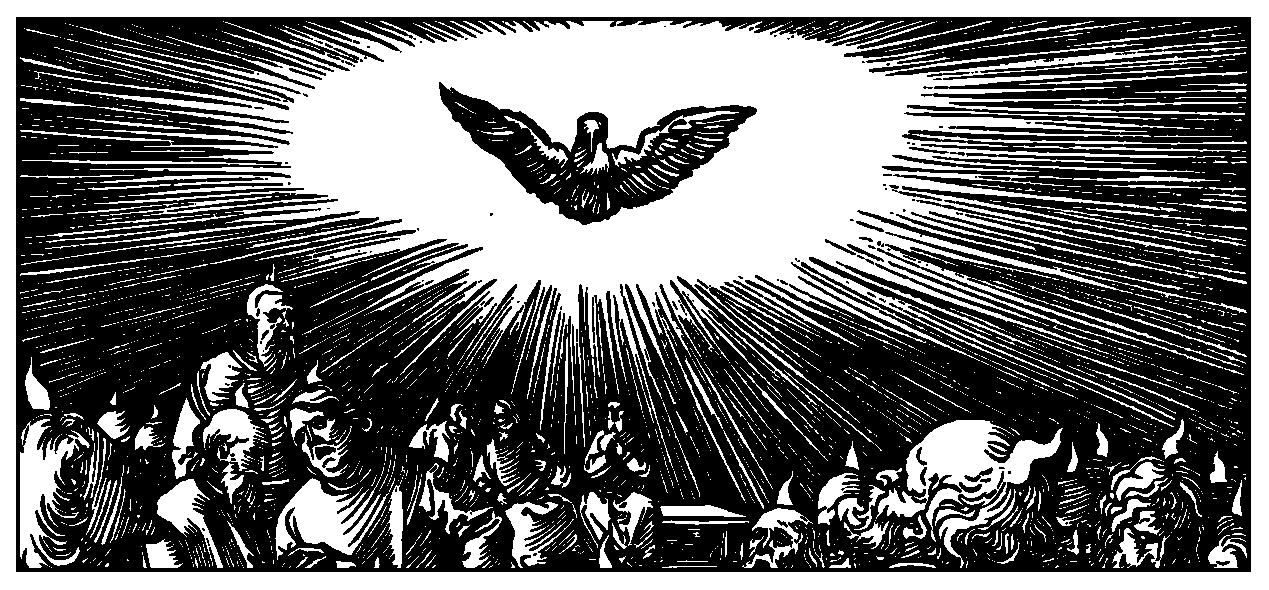
\includegraphics[width=95mm,height=42.706mm]{tailpiece/Whitsunday.eps}
\end{figure}
%MANUAL ADJUSTMENT:
\clearpage
\subsection{Whit-Monday}
\feastday{Whit-Monday}
\begin{inhead}
    {First Class Double}
\end{inhead}

%\properantiphonfix

\introit
\lett{H}{e} fed them with the finest wheat-flour, alleluia: and with honey out of the stony rock hath he satisfied them, alleluia, alleluia. \textit{Ps.} Sing we merrily unto God our strength: make a cheerful noise unto the God of Jacob.
\collect
\lett{S}{end,} we beseech thee, Almighty God, thy Holy Spirit into our hearts, that he may direct and rule us according to thy will, comfort us in all our afflictions, defend us from all error, and lead us into all truth; through Jesus Christ our Lord, who with thee and the same Holy Spirit liveth and reigneth, one God, world without end. \textit{Amen.}
\readingcitation{Epistle}{Acts 10:34}
\lett{I}{n those days:} Peter opened his mouth, and said, Of a truth I perceive that God is no respecter of persons: But in every nation he that feareth him, and worketh righteousness, is accepted with him. The word which God sent unto the children of Israel, preaching peace by Jesus Christ: (he is Lord of all:) That word, I say, ye know, which was published throughout all Judaea, and began from Galilee, after the baptism which John preached; How God anointed Jesus of Nazareth with the Holy Ghost and with power: who went about doing good, and healing all that were oppressed of the devil; for God was with him. And we are witnesses of all things which he did both in the land of the Jews, and in Jerusalem; whom they slew and hanged on a tree: Him God raised up the third day, and shewed him openly; Not to all the people, but unto witnesses chosen before of God, even to us, who did eat and drink with him after he rose from the dead. And he commanded us to preach unto the people, and to testify that it is he which was ordained of God to be the Judge of quick and dead. To him give all the prophets witness, that through his name whosoever believeth in him shall receive remission of sins. While Peter yet spake these words, the Holy Ghost fell on all them which heard the word. And they of the circumcision which believed were astonished, as many as came with Peter, because that on the Gentiles also was poured out the gift of the Holy Ghost. For they heard them speak with tongues, and magnify God. Then answered Peter, Can any man forbid water, that these should not be baptized, which have received the Holy Ghost as well as we? And he commanded them to be baptized in the name of the Lord. Then prayed they him to tarry certain days.

\alleluia{Alleluia, alleluia. ℣. The Apostles spake with other tongues the wonderful works of God, alleluia. \inrub{Here genuflect.} ℣. Come, Holy Ghost, fill the hearts of thy faithful: and kindle in them the fire of thy love.}
\begin{rubric}
{The Sequence as on Whit-Sunday (p. \pageref{WhitSeq})}
\end{rubric}
\readingcitation{Gospel}{John 3:16}
\lett{A}{t that time:} Jesus said unto Nicodemus: God so loved the world, that he gave his only begotten Son, that whosoever believeth in him should not perish, but have everlasting life. For God sent not his Son into the world to condemn the world; but that the world through him might be saved. He that believeth on him is not condemned: but he that believeth not is condemned already, because he hath not believed in the name of the only begotten Son of God. And this is the condemnation, that light is come into the world, and men loved darkness rather than light, because their deeds were evil. For every one that doeth evil hateth the light, neither cometh to the light, lest his deeds should be reproved. But he that doeth truth cometh to the light, that his deeds may be made manifest, that they are wrought in God.
\offertory{The Lord thundered out of heaven, and the Highest gave forth his voice: and the springs of waters were seen, alleluia.}
\secret
\lett{W}{e} beseech thee, O Lord, graciously to sanctify these gifts: and by the acceptable offering of our spiritual sacrifice, render us ourselves an everlasting oblation unto thee. Through.
\communion{The Holy Ghost shall teach you, alleluia: whatsoever I have said unto you, alleluia, alleluia.}
\postcommunion
\lett{A}{ssist,} O Lord, we beseech thee, thy people: and defend from the fury of their enemies those whom thou hast fulfilled with heavenly mysteries. Through.


%MANUAL ADJUSTMENT:
\clearpage
\subsection{Whit-Tuesday}
\feastday{Whit-Tuesday}
\begin{inhead}
    {First Class Double}
\end{inhead}

%\properantiphonfix

\introit
\lett{R}{eceive} the joyfulness of your glory, alleluia: giving thanks unto God, alleluia: who hath called you to the heavenly kingdom, alleluia, alleluia, alleluia. \textit{Ps.} Hear my law, O my people: incline your ears unto the words of my mouth.
\collect
\lett{G}{rant,} we beseech thee, merciful God, that thy Church, being gathered together in unity by thy Holy Spirit, may manifest thy power among all peoples, to the glory of thy Name; through Jesus Christ our Lord, who liveth and reigneth with thee and the same Spirit, one God, world without end. \textit{Amen.}

\readingcitation{Epistle}{Acts 8:14}
\lett{I}{n those days:} When the apostles which were at Jerusalem heard that Samaria had received the word of God, they sent unto them Peter and John: Who, when they were come down, prayed for them, that they might receive the Holy Ghost: (For as yet he was fallen upon none of them: only they were baptized in the name of the Lord Jesus.) Then laid they their hands on them, and they received the Holy Ghost.
\alleluia{Alleluia, alleluia, ℣. The Holy Ghost shall teach you, whatsoever I have said unto you. Alleluia. \inrub{Here genuflect.} ℣. Come, Holy Ghost, fill the hearts of thy faithful: and kindle in them the fire of thy love.}
\begin{rubric}
{The Sequence as on Whit-Sunday (p. \pageref{WhitSeq})}
\end{rubric}

\readingcitation{Gospel}{John 10:1}
\lett{A}{t that time:} Jesus said unto the Pharisees: Verily, verily, I say unto you, He that entereth not by the door into the sheepfold, but climbeth up some other way, the same is a thief and a robber. But he that entereth in by the door is the shepherd of the sheep. To him the porter openeth; and the sheep hear his voice: and he calleth his own sheep by name, and leadeth them out. And when he putteth forth his own sheep, he goeth before them, and the sheep follow him: for they know his voice. And a stranger will they not follow, but will flee from him: for they know not the voice of strangers. This parable spake Jesus unto them: but they understood not what things they were which he spake unto them. Then said Jesus unto them again, Verily, verily, I say unto you, I am the door of the sheep. All that ever came before me are thieves and robbers: but the sheep did not hear them. I am the door: by me if any man enter in, he shall be saved, and shall go in and out, and find pasture. The thief cometh not, but for to steal, and to kill, and to destroy: I am come that they might have life, and that they might have it more abundantly.
\offertory{The Lord opened the doors of heaven: he rained down manna also upon them for to eat: he gave them food from heaven, so man did eat Angels' food, alleluia.}

\secret
\lett{M}{ay} the offering of this gift purify us, we beseech thee, O Lord: and render us worthy to partake of holy things. Through.

\lettspace

\communion{The Spirit which proceedeth from the Father, alleluia: he shall glorify me, alleluia, alleluia.}

\postcommunion
\lett{W}{e} beseech thee, O Lord, that the Holy Ghost may renew our minds by divine sacraments: forasmuch as he is himself the remission of all sins. Through.


%MANUAL ADJUSTMENT:
\clearpage
\subsection{Ember Wednesday in Whitsuntide}
\feastday{Whitsun Emberday}
\begin{inhead}
    {Semidouble}
\end{inhead}
\fancyhead[RE,LO]{Ember Wednesday}

\introit
\lett{O}{God,} when thou wentest forth before the people, journeying and dwelling with them, alleluia: the earth shook, and the heavens dropped, alleluia, alleluia. \textit{Ps.} Let God arise, and let his enemies be scattered: let them also that hate him flee before him.

\begin{rubric}
	After the \blackrubric{Kyrie,} is said \blackrubric{Let us pray,} then the following.
\end{rubric}

\collect
\lett{W}{e} beseech thee, O Lord, that the Paraclete, who proceedeth from thee, may enlighten our minds: and lead us, as thy Son hath promised, into all truth; Who liveth.

\readingcitation{Epistle}{Acts 2:14}
\lett{I}{n those days:} Peter, standing up with the eleven, lifted up his voice, and said unto them, Ye men of Judaea, and all ye that dwell at Jerusalem, be this known unto you, and hearken to my words: For these are not drunken, as ye suppose, seeing it is but the third hour of the day. But this is that which was spoken by the prophet Joel; And it shall come to pass in the last days, saith God, I will pour out of my Spirit upon all flesh: and your sons and your daughters shall prophesy, and your young men shall see visions, and your old men shall dream dreams: And on my servants and on my handmaidens I will pour out in those days of my Spirit; and they shall prophesy: And I will shew wonders in heaven above, and signs in the earth beneath; blood, and fire, and vapour of smoke: The sun shall be turned into darkness, and the moon into blood, before that great and notable day of the Lord come: And it shall come to pass, that whosoever shall call on the name of the Lord shall be saved.

\alleluia{Alleluia. ℣. By the word of the Lord were the heavens made, and all the hosts of them by the breath of his mouth.}

\begin{rubric}
	Here is said \blackrubric{Gloria in excelsis,} and then \blackrubric{The Lord be with you.}
\end{rubric}

\collect
\lett{G}{rant,} we beseech thee, Almighty and Merciful God: that the Holy Ghost descending on us may by his gracious indwelling render us a temple of his glory. Through.

\begin{rubric}
    From this day until the Saturday following, inclusive, after the Collect of the Day is said the \nth{2} \blackrubric{Against the Persecutors of the Church} (p. \pageref{SPAgainst}) or \blackrubric{for the Chief Bishop} (p. \pageref{SPChiefBishop}).
\end{rubric}

\readingcitation{Epistle}{Acts 5:12}
\lett{I}{n those days:} By the hands of the apostles were many signs and wonders wrought among the people; (and they were all with one accord in Solomon's porch. And of the rest durst no man join himself to them: but the people magnified them. And believers were the more added to the Lord, multitudes both of men and women.) Insomuch that they brought forth the sick into the streets, and laid them on beds and couches, that at the least the shadow of Peter passing by might overshadow some of them. There came also a multitude out of the cities round about unto Jerusalem, bringing sick folks, and them which were vexed with unclean spirits: and they were healed every one.

\alleluia{Alleluia, alleluia. \inrub{Here genuflect.} ℣. Come, Holy Ghost, fill the hearts of thy faithful: and kindle in them the fire of thy love.}

\begin{rubric}
{The Sequence as on Whit-Sunday (p. \pageref{WhitSeq})}
\end{rubric}

\readingcitation{Gospel}{John 6:44}
\lett{A}{t that time}: Jesus said to the multitudes of the Jews: No man can come to me, except the Father which hath sent me draw him: and I will raise him up at the last day. It is written in the prophets, And they shall be all taught of God. Every man therefore that hath heard, and hath learned of the Father, cometh unto me. Not that any man hath seen the Father, save he which is of God, he hath seen the Father. Verily, verily, I say unto you, He that believeth on me hath everlasting life. I am that bread of life. Your fathers did eat manna in the wilderness, and are dead. This is the bread which cometh down from heaven, that a man may eat thereof, and not die. I am the living bread which came down from heaven: if any man eat of this bread, he shall live for ever: and the bread that I will give is my flesh, which I will give for the life of the world.

\offertory{My delight shall be in thy commandments, which I have loved exceedingly: my hands also will I lift up unto thy commandments, which I have loved, alleluia.}

\secret
\lett{A}{ccept,} we beseech thee, O Lord, the gift which we offer: and vouchsafe so to work, that what we perform in a mystery, we may celebrate with godly devotion. Through.
\begin{rubric}
    \nth{2} Secret \blackrubric{Against the Persecutors of the Church} (p. \pageref{SPAgainst}) or \blackrubric{for the Chief Bishop} (p. \pageref{SPChiefBishop}).
\end{rubric}

\communion{Peace I leave with you, alleluia: my peace I give unto you, alleluia, alleluia.}

\postcommunion
\lett{W}{e,} O Lord, who receive the heavenly sacraments, beseech thy mercy: that by those things which we perform in this life we may attain unto everlasting joys. Through.
\begin{rubric}
    \nth{2} Postcommunion \blackrubric{Against the Persecutors of the Church} (p. \pageref{SPAgainst}) or \blackrubric{for the Chief Bishop} (p. \pageref{SPChiefBishop}).
\end{rubric}


\subsection{Whit-Thursday}
\feastday{Whit-Thursday}
\begin{inhead}
    {Semidouble}
\end{inhead}
\fancyhead[RE,LO]{}

%\properantiphonfix

\introit
\lett{T}{he} Spirit of the Lord hath filled the whole world, alleluia: and that which containeth all things hath knowledge of the voice, alleluia, alleluia, alleluia. \textit{Ps.} Let God arise, and let his enemies be scattered: let them also that hate him flee before him.
\collect
\lett{G}{od,} who as at this time didst teach the hearts of thy faithful people, by sending to them the light of thy Holy Spirit; grant us by the same Spirit to have a right judgment in all things, and evermore to rejoice in his holy comfort. Through.
\begin{rubric}
    \nth{2} Collect \blackrubric{Against the Persecutors of the Church} (p. \pageref{SPAgainst}) or \blackrubric{for the Chief Bishop} (p. \pageref{SPChiefBishop}).
\end{rubric}
\readingcitation{Epistle}{Acts 8:5}
\lett{I}{n those days:} Philip went down to the city of Samaria, and preached Christ unto them. And the people with one accord gave heed unto those things which Philip spake, hearing and seeing the miracles which he did. For unclean spirits, crying with loud voice, came out of many that were possessed with them: and many taken with palsies, and that were lame, were healed. And there was great joy in that city.
\alleluia{Alleluia, alleluia, ℣. O send forth thy Spirit, and they shall be made: and thou shalt renew the face of the earth. Alleluia. \inrub{Here genuflect.} ℣. Come, Holy Ghost, fill the hearts of thy faithful: and kindle in them the fire of thy love.}
\begin{rubric}
{The Sequence as on Whit-Sunday (p. \pageref{WhitSeq})}
\end{rubric}
\readingcitation{Gospel}{Luke 9:1}
\lett{A}{t that time:} Jesus called his twelve disciples together, and gave them power and authority over all devils, and to cure diseases. And he sent them to preach the kingdom of God, and to heal the sick. And he said unto them, Take nothing for your journey, neither staves, nor scrip, neither bread, neither money; neither have two coats apiece. And whatsoever house ye enter into, there abide, and thence depart. And whosoever will not receive you, when ye go out of that city, shake off the very dust from your feet for a testimony against them. And they departed, and went through the towns, preaching the gospel, and healing every where.
\offertory{Stablish the thing, O God, that thou hast wrought in us: for thy temple's sake at Jerusalem shall kings bring presents unto thee, alleluia.}
\secret
\lett{S}{anctify,} we beseech thee, O Lord, the gifts which we offer: and cleanse our hearts by the enlightening of the Holy Spirit. Through.

\lettspace

\begin{rubric}
    \nth{2} Secret \blackrubric{Against the Persecutors of the Church} (p. \pageref{SPAgainst}) or \blackrubric{for the Chief Bishop} (p. \pageref{SPChiefBishop}).
\end{rubric}
\communion{Suddenly there came a sound from heaven, as of a rushing mighty wind, where they were sitting, alleluia: and they were all filled with the Holy Ghost speaking the wonderful works of God, alleluia, alleluia.}

\postcommunion
\lett{P}{our} thy Holy Spirit upon us, O Lord, and cleanse our hearts: that they may be made fruitful by the inward sprinkling of his dew. Through.

\lettspace

\begin{rubric}
    \nth{2} Postcommunion \blackrubric{Against the Persecutors of the Church} (p. \pageref{SPAgainst}) or \blackrubric{for the Chief Bishop} (p. \pageref{SPChiefBishop}).
\end{rubric}


\subsection{Ember Friday in Whitsuntide}
\feastday{Whitsun Emberday}
\begin{inhead}
    {Semidouble}
\end{inhead}
\fancyhead[RE,LO]{Ember Friday}

\introit
\lett{O}{Let} my mouth be filled with thy praise, alleluia: that I may sing, alleluia: my lips will be fain when I sing unto thee, alleluia, alleluia. \textit{Ps.} In thee, O Lord, have I put my trust, let me never be put to confusion: but rid me, and deliver me in thy righteousness.

\collect
\lett{G}{rant,} we beseech thee, O merciful God, to thy Church: that, being gathered together in the Holy Ghost, she may be disturbed by no assaults of the enemy. Through.
\begin{rubric}
    \nth{2} Collect \blackrubric{Against the Persecutors of the Church} (p. \pageref{SPAgainst}) or \blackrubric{for the Chief Bishop} (p. \pageref{SPChiefBishop}).
\end{rubric}

\readingcitation{Epistle}{Joel 2:23}
\lett{T}{hus saith the Lord God:} Be glad then, ye children of Zion, and rejoice in the \divineName{Lord} your God: for he hath given you the former rain moderately, and he will cause to come down for you the rain, the former rain, and the latter rain in the first month. And the floors shall be full of wheat, and the fats shall overflow with wine and oil. And I will restore to you the years that the locust hath eaten, the cankerworm, and the caterpiller, and the palmerworm, my great army which I sent among you. And ye shall eat in plenty, and be satisfied, and praise the name of the \divineName{Lord} your God, that hath dealt wondrously with you: and my people shall never be ashamed. And ye shall know that I am in the midst of Israel, and that I am the \divineName{Lord} your God, and none else: and my people shall never be ashamed, saith the Lord Almighty.

\alleluia{Alleluia, alleluia. ℣. O how good and sweet, O Lord, is thy Spirit within us. Alleluia. \inrub{Here genuflect.} ℣. Come, Holy Ghost, fill the hearts of thy faithful: and kindle in them the fire of thy love.}
\begin{rubric}
{The Sequence as on Whit-Sunday (p. \pageref{WhitSeq})}
\end{rubric}

\readingcitation{Gospel}{Luke 5:17}
\lett{A}{t that time:} And it came to pass on a certain day, as Jesus was teaching, that there were Pharisees and doctors of the law sitting by, which were come out of every town of Galilee, and Judaea, and Jerusalem: and the power of the Lord was present to heal them. And, behold, men brought in a bed a man which was taken with a palsy: and they sought means to bring him in, and to lay him before him. And when they could not find by what way they might bring him in because of the multitude, they went upon the housetop, and let him down through the tiling with his couch into the midst before Jesus. And when he saw their faith, he said unto him, Man, thy sins are forgiven thee. And the scribes and the Pharisees began to reason, saying, Who is this which speaketh blasphemies? Who can forgive sins, but God alone? But when Jesus perceived their thoughts, he answering said unto them, What reason ye in your hearts? Whether is easier, to say, Thy sins be forgiven thee; or to say, Rise up and walk? But that ye may know that the Son of man hath power upon earth to forgive sins, (he said unto the sick of the palsy,) I say unto thee, Arise, and take up thy couch, and go into thine house. And immediately he rose up before them, and took up that whereon he lay, and departed to his own house, glorifying God. And they were all amazed, and they glorified God, and were filled with fear, saying, We have seen strange things to day.
\offertory{Praise the Lord, O my soul: while I live will I praise the Lord: yea, as long as I have any being, I will sing praises unto my God, alleluia.}
\secret
\lett{M}{ay} the sacrifices, which we offer in thy sight, O Lord, be consumed by that divine fire, which through the Holy Spirit enkindled the hearts of the disciples of Christ, thy Son. Through the same.
\begin{rubric}
    \nth{2} Secret \blackrubric{Against the Persecutors of the Church} (p. \pageref{SPAgainst}) or \blackrubric{for the Chief Bishop} (p. \pageref{SPChiefBishop}).
\end{rubric}

\communion{I will not leave you comfortless: I will come to you again, alleluia: and your heart shall rejoice, alleluia.}
\postcommunion
\lett{W}{e} have received, O Lord, the gifts of thy sacred mystery: humbly beseeching thee; that those things which thou hast commanded us to do in remembrance of thee, may be profitable to the succour of our infirmity. Who livest.
\begin{rubric}
    \nth{2} Postcommunion \blackrubric{Against the Persecutors of the Church} (p. \pageref{SPAgainst}) or \blackrubric{for the Chief Bishop} (p. \pageref{SPChiefBishop}).
\end{rubric}


\subsection{Ember Saturday in Whitsuntide}
\feastday{Whitsun Emberday}
\begin{inhead}
    {Semidouble}
\end{inhead}
\fancyhead[RE,LO]{Ember Saturday}

\introit
\lett{T}{he} love of God is shed abroad in our hearts, alleluia: by the Holy Ghost which dwelleth in us, alleluia, alleluia. \textit{Ps.} Praise the Lord, O my soul: and all that is within me, praise his holy name.

\begin{rubric}
	After the \blackrubric{Kyrie,} is said \blackrubric{Let us pray,} then the following.
\end{rubric}

\collect
\lett{W}{e} beseech thee, O Lord, graciously pour the Holy Ghost into our hearts: by whose wisdom we were created, and by whose providence we are governed. Through.

\readingcitation{Epistle}{Joel 2:28}
\lett{T}{hus saith the Lord God:} I will pour out my spirit upon all flesh; and your sons and your daughters shall prophesy, your old men shall dream dreams, your young men shall see visions: And also upon the servants and upon the handmaids in those days will I pour out my spirit. And I will shew wonders in the heavens and in the earth, blood, and fire, and pillars of smoke. The sun shall be turned into darkness, and the moon into blood, before the great and the terrible day of the \divineName{Lord} come. And it shall come to pass, that whosoever shall call on the name of the \divineName{Lord} shall be delivered.

\alleluia{Alleluia. ℣. It is the spirit that quickeneth: the flesh profiteth nothing.}

\collect
\letuspray
\lett{W}{e} beseech thee, O Lord, that the Holy Ghost may inflame us with that fire: which our Lord Jesus Christ sent upon earth, and willed that it should be kindled exceedingly. Who liveth.

\readingcitation{Epistle}{Leviticus 23:9}
\lett{I}{n those days:} The \divineName{Lord} spake unto Moses, saying, Speak unto the children of Israel, and say unto them, When ye be come into the land which I give unto you, and shall reap the harvest thereof, then ye shall bring a sheaf of the firstfruits of your harvest unto the priest: And he shall wave the sheaf before the \divineName{Lord}, to be accepted for you: on the morrow after the sabbath the priest shall wave it. And ye shall offer that day when ye wave the sheaf an he lamb without blemish of the first year for a burnt offering unto the \divineName{Lord}. And the meat offering thereof shall be two tenth deals of fine flour mingled with oil, an offering made by fire unto the \divineName{Lord} for a sweet savour: and the drink offering thereof shall be of wine, the fourth part of an hin. And ye shall eat neither bread, nor parched corn, nor green ears, until the selfsame day that ye have brought an offering unto your God: it shall be a statute for ever throughout your generations in all your dwellings. And ye shall count unto you from the morrow after the sabbath, from the day that ye brought the sheaf of the wave offering; seven sabbaths shall be complete: Even unto the morrow after the seventh sabbath shall ye number fifty days; and ye shall offer a new meat offering unto the \divineName{Lord}. Ye shall bring out of your habitations two wave loaves of two tenth deals: they shall be of fine flour; they shall be baken with leaven; they are the firstfruits unto the \divineName{Lord}. And ye shall offer with the bread seven lambs without blemish of the first year, and one young bullock, and two rams: they shall be for a burnt offering unto the \divineName{Lord}, with their meat offering, and their drink offerings, even an offering made by fire, of sweet savour unto the \divineName{Lord}. Then ye shall sacrifice one kid of the goats for a sin offering, and two lambs of the first year for a sacrifice of peace offerings. And the priest shall wave them with the bread of the firstfruits for a wave offering before the \divineName{Lord}, with the two lambs: they shall be holy to the \divineName{Lord} for the priest. And ye shall proclaim on the selfsame day, that it may be an holy convocation unto you: ye shall do no servile work therein: it shall be a statute for ever in all your dwellings throughout your generations, saith the Lord almighty.

\alleluia{Alleluia. ℣. By his Spirit he hath garnished the heavens.}

\collect
\letuspray
\lett{O}{God,} who for the healing of our souls hast commanded us to chasten our bodies with godly fasting: mercifully grant unto us: that we may ever serve thee both in body and soul. Through.

%MANUAL ADJUSTMENT:
\vspace{-0.33\baselineskip}

\readingcitation{Epistle}{Deuteronomy 26:1}

%MANUAL ADJUSTMENT:
\vspace{-0.1515\baselineskip}

\lett{I}{n those days:} Moses said to the children of Israel: Hear, O Israel, what I command thee this day. When thou art come in unto the land which the \divineName{Lord} thy God giveth thee for an inheritance, and possessest it, and dwellest therein; That thou shalt take of the first of all the fruit of the earth, which thou shalt bring of thy land that the \divineName{Lord} thy God giveth thee, and shalt put it in a basket, and shalt go unto the place which the \divineName{Lord} thy God shall choose to place his name there. And thou shalt go unto the priest that shall be in those days, and say unto him, I profess this day unto the \divineName{Lord} thy God, that I am come unto the country which the \divineName{Lord} sware unto our fathers for to give us. And the priest shall take the basket out of thine hand, and set it down before the altar of the \divineName{Lord} thy God. And thou shalt speak and say before the \divineName{Lord} thy God, A Syrian ready to perish was my father, and he went down into Egypt, and sojourned there with a few, and became there a nation, great, mighty, and populous: And the Egyptians evil entreated us, and afflicted us, and laid upon us hard bondage: And when we cried unto the \divineName{Lord} God of our fathers, the \divineName{Lord} heard our voice, and looked on our affliction, and our labour, and our oppression: And the \divineName{Lord} brought us forth out of Egypt with a mighty hand, and with an outstretched arm, and with great terribleness, and with signs, and with wonders: And he hath brought us into this place, and hath given us this land, even a land that floweth with milk and honey. And now, behold, I have brought the firstfruits of the land, which thou, O \divineName{Lord}, hast given me. And thou shalt set it before the \divineName{Lord} thy God, and worship before the \divineName{Lord} thy God: And thou shalt rejoice in every good thing which the \divineName{Lord} thy God hath given unto thee.

\alleluia{Alleluia. ℣. When the day of Pentecost was fully come, they were all sitting with one accord.}

%MANUAL ADJUSTMENT:
\vspace{-0.34\baselineskip}

\collect

%MANUAL ADJUSTMENT:
\vspace{-0.1515\baselineskip}

\letuspray
\lett{G}{rant,} we beseech thee, almighty God: that we, being taught by these saving fasts, and likewise abstaining from all vices, may more readily obtain thy pardon. Through.

\readingcitation{Epistle}{Leviticus 26:3}
\lett{I}{n those days:} The Lord said unto Moses: Speak unto the children of Israel, and say unto them: If ye walk in my statutes, and keep my commandments, and do them; Then I will give you rain in due season, and the land shall yield her increase, and the trees of the field shall yield their fruit. And your threshing shall reach unto the vintage, and the vintage shall reach unto the sowing time: and ye shall eat your bread to the full, and dwell in your land safely. And I will give peace in the land, and ye shall lie down, and none shall make you afraid: and I will rid evil beasts out of the land, neither shall the sword go through your land. And ye shall chase your enemies, and they shall fall before you by the sword. And five of you shall chase an hundred, and an hundred of you shall put ten thousand to flight: and your enemies shall fall before you by the sword. For I will have respect unto you, and make you fruitful, and multiply you, and establish my covenant with you. And ye shall eat old store, and bring forth the old because of the new. And I will set my tabernacle among you: and my soul shall not abhor you. And I will walk among you, and will be your God, and ye shall be my people, saith the Lord almighty.

\alleluia{Alleluia. \inrub{Here genuflect.} ℣. Come, Holy Ghost, fill the hearts of thy faithful: and kindle in them the fire of thy love.}

\collect
\letuspray
\lett{G}{rant,} we beseech thee, Almighty God: that we may so abstain from carnal feasting; that we may likewise fast from the vices which beset us. Through.

\readingcitation{Epistle}{Song of the Three Children 26}
\lett{I}{n those days:} The Angel of the Lord came down into the oven together with Azarias and his fellows, and smote the flame of the fire out of the oven; And made the midst of the furnace as it had been a moist whistling wind, so that the fire touched them not at all, neither hurt nor troubled them. Then the three, as out of one mouth, praised, glorified, and blessed, God in the furnace, saying,

\begin{rubric}
    Here the response \blackrubric{Thanks be to God,} is not made.
\end{rubric}

\alleluia{Alleluia. ℣. Blessed art thou, O Lord, God of our Fathers, and worthy to be praised for ever.}

\begin{rubric}
	Here is said \blackrubric{Gloria in excelsis,} and then \blackrubric{The Lord be with you.}
\end{rubric}

\collect
\letuspray
\lett{O}{God,} who to the three children didst assuage the flames of fire; mercifully grant; that the flames of sin may not kindle upon us thy servants. Through.
\begin{rubric}
    \nth{2} Collect \blackrubric{Against the Persecutors of the Church} (p. \pageref{SPAgainst}) or \blackrubric{for the Chief Bishop} (p. \pageref{SPChiefBishop}).
\end{rubric}

\readingcitation{Epistle}{Romans 5:1}
\lett{B}{rethren:} Being justified by faith, we have peace with God through our Lord Jesus Christ: By whom also we have access by faith into this grace wherein we stand, and rejoice in hope of the glory of God. And not only so, but we glory in tribulations also: knowing that tribulation worketh patience; And patience, experience; and experience, hope: And hope maketh not ashamed; because the love of God is shed abroad in our hearts by the Holy Ghost which is given unto us.

\tract{O praise the Lord, all ye heathen: praise him, all ye nations, ℣. For his merciful kindness is ever more and more towards us: and the truth of the Lord endureth for ever.}

\begin{rubric}
{The Sequence as on Whit-Sunday (p. \pageref{WhitSeq})}
\end{rubric}

\begin{rubric}
    \textsc{Note,} At the end, \blackrubric{Alleluia} is not said.
\end{rubric}

\readingcitation{Gospel}{Luke 4:38}
\lett{A}{t that time:} Jesus arose out of the synagogue, and entered into Simon's house. And Simon's wife's mother was taken with a great fever; and they besought him for her. And he stood over her, and rebuked the fever; and it left her: and immediately she arose and ministered unto them. Now when the sun was setting, all they that had any sick with divers diseases brought them unto him; and he laid his hands on every one of them, and healed them. And devils also came out of many, crying out, and saying, Thou art Christ the Son of God. And he rebuking them suffered them not to speak: for they knew that he was Christ. And when it was day, he departed and went into a desert place: and the people sought him, and came unto him, and stayed him, that he should not depart from them. And he said unto them, I must preach the kingdom of God to other cities also: for therefore am I sent. And he preached in the synagogues of Galilee.

\offertory{O Lord God of my salvation, I have cried day and night before thee: let my prayer enter into thy presence, O Lord, alleluia.}

\secret
\lett{T}{hat} our fasts may be acceptable to thee, O Lord: grant us, we beseech thee: by the gift of this sacrament to offer unto thee a purified heart. Through.
\begin{rubric}
    \nth{2} Secret \blackrubric{Against the Persecutors of the Church} (p. \pageref{SPAgainst}) or \blackrubric{for the Chief Bishop} (p. \pageref{SPChiefBishop}).
\end{rubric}

\communion{The Spirit bloweth where it listeth; and thou hearest the sound thereof, alleluia, alleluia: but canst not tell whence it cometh and whither it goeth, alleluia, alleluia, alleluia.}

\postcommunion
\lett{M}{ay} thy holy things, O Lord, impart to us divine fervour: that we may delight both in the performance and likewise in the fulfilment of the same. Through.
\begin{rubric}
    \nth{2} Postcommunion \blackrubric{Against the Persecutors of the Church} (p. \pageref{SPAgainst}) or \blackrubric{for the Chief Bishop} (p. \pageref{SPChiefBishop}).
\end{rubric}

\begin{rubric}
	\textsc{Note,} After the Mass, Eastertide ends.
\end{rubric}



%TAILPIECE
\vfill

\begin{figure}[H]
    \centering
    
\includegraphics[width=103mm,height=55.030mm]{tailpiece/Trinity.eps}
\end{figure}

%MANUAL ADJUSTMENT:
\clearpage

\section{Trinitytide}

\subsection{Trinity Sunday}
\feastday{Trinity Sunday}
\begin{inhead}
    {First Class Double}
\end{inhead}
\fancyhead[RE,LO]{}

%\properantiphonfix

\introit
\lett{B}{lessed} be the holy Trinity, and the undivided Unity: we will praise and glorify him, because he hath showed his mercy upon us. \textit{Ps.} O Lord our governor: how excellent is thy name in all the world!
\collect
\lett{A}{lmighty} and everlasting God, who hast given unto us thy servants grace by the confession of a true faith to acknowledge the glory of the eternal Trinity, and in the power of the Divine Majesty to worship the Unity: We beseech thee; that thou wouldest keep us stedfast in this faith, and evermore defend us from all adversities. Who livest and reignest, one God, world without end. \textit{Amen.}

\readingcitation{Epistle}{Revelation 4:1}
\lett{I}{n those days:} I looked, and, behold, a door was opened in heaven: and the first voice which I heard was as it were of a trumpet talking with me; which said, Come up hither, and I will shew thee things which must be hereafter. And immediately I was in the spirit: and, behold, a throne was set in heaven, and one sat on the throne. And he that sat was to look upon like a jasper and a sardine stone: and there was a rainbow round about the throne, in sight like unto an emerald. And round about the throne were four and twenty seats: and upon the seats I saw four and twenty elders sitting, clothed in white raiment; and they had on their heads crowns of gold. And out of the throne proceeded lightnings and thunderings and voices: and there were seven lamps of fire burning before the throne, which are the seven Spirits of God. And before the throne there was a sea of glass like unto crystal: and in the midst of the throne, and round about the throne, were four beasts full of eyes before and behind. And the first beast was like a lion, and the second beast like a calf, and the third beast had a face as a man, and the fourth beast was like a flying eagle. And the four beasts had each of them six wings about him; and they were full of eyes within: and they rest not day and night, saying, Holy, holy, holy, Lord God Almighty, which was, and is, and is to come. And when those beasts give glory and honour and thanks to him that sat on the throne, who liveth for ever and ever, The four and twenty elders fall down before him that sat on the throne, and worship him that liveth for ever and ever, and cast their crowns before the throne, saying, Thou art worthy, O Lord, to receive glory and honour and power: for thou hast created all things, and for thy pleasure they are and were created.

\gradall{Blessed art thou, O Lord, that beholdest the depths, and sittest upon the Cherubim. ℣. Blessed art thou, O Lord, in the firmament of heaven, and worthy to be praised for ever.}{Alleluia, alleluia. ℣. Blessed art thou, O Lord God of our fathers, and worthy to be praised for evermore. Alleluia.}

\readingcitation{Gospel}{John 3:1}
\lett{A}{t that time:} There was a man of the Pharisees, named Nicodemus, a ruler of the Jews: The same came to Jesus by night, and said unto him, Rabbi, we know that thou art a teacher come from God: for no man can do these miracles that thou doest, except God be with him. Jesus answered and said unto him, Verily, verily, I say unto thee, Except a man be born again, he cannot see the kingdom of God. Nicodemus saith unto him, How can a man be born when he is old? can he enter the second time into his mother's womb, and be born? Jesus answered, Verily, verily, I say unto thee, Except a man be born of water and of the Spirit, he cannot enter into the kingdom of God. That which is born of the flesh is flesh; and that which is born of the Spirit is spirit. Marvel not that I said unto thee, Ye must be born again. The wind bloweth where it listeth, and thou hearest the sound thereof, but canst not tell whence it cometh, and whither it goeth: so is every one that is born of the Spirit. Nicodemus answered and said unto him, How can these things be? Jesus answered and said unto him, Art thou a master of Israel, and knowest not these things? Verily, verily, I say unto thee, We speak that we do know, and testify that we have seen; and ye receive not our witness. If I have told you earthly things, and ye believe not, how shall ye believe, if I tell you of heavenly things? And no man hath ascended up to heaven, but he that came down from heaven, even the Son of man which is in heaven. And as Moses lifted up the serpent in the wilderness, even so must the Son of man be lifted up: That whosoever believeth in him should not perish, but have eternal life.

\offertory{Blessed be God the Father, and the only-begotten Son of God, and the Holy Spirit: because he hath showed his mercy upon us.}

\secret
\lett{S}{anctify,} we beseech thee, O Lord our God, the sacrifice which we here offer by the invocation of thy holy name: that through the same we may ourselves be made a perfect gift unto thee for evermore. Through.
%Secret is said on Trinity I, so no need for commemoration today.
%
%\lett{D}{o} thou, we beseech thee, O Lord, graciously accept the offerings which have been dedicated unto thee: and grant that they may become to us an abiding source of strength. Through.
\communion{We bless the God of heaven, and will praise him in the sight of all that live: because he hath showed his mercy upon us.}
\postcommunion
\lett{G}{rant,} O Lord our God: that we who receive this sacrament and who acknowledge the holy and everlasting Trinity, and likewise the undivided Unity: may be profited thereby unto salvation of body and soul. Through.
%Collect is said on Trinity I, so no need for commemoration today.
%
%\lett{G}{rant,} we beseech thee, O Lord, that we, who have been filled with such great gifts, may both receive these gifts unto our profit, and never cease from thy praise. Through.
%In the English tradition, this is moved to Trinity IV
%\readingcitation{Last Gospel}{Luke 6:36}
%\lett{A}{t that time:} Jesus said unto his disciples: Be ye therefore merciful, as your Father also is merciful. Judge not, and ye shall not be judged: condemn not, and ye shall not be condemned: forgive, and ye shall be forgiven: Give, and it shall be given unto you; good measure, pressed down, and shaken together, and running over, shall men give into your bosom. For with the same measure that ye mete withal it shall be measured to you again. And he spake a parable unto them, Can the blind lead the blind? shall they not both fall into the ditch? The disciple is not above his master: but every one that is perfect shall be as his master. And why beholdest thou the mote that is in thy brother's eye, but perceivest not the beam that is in thine own eye? Either how canst thou say to thy brother, Brother, let me pull out the mote that is in thine eye, when thou thyself beholdest not the beam that is in thine own eye? Thou hypocrite, cast out first the beam out of thine own eye, and then shalt thou see clearly to pull out the mote that is in thy brother's eye.

\subsection{The Most Holy Body of Christ}
\feastday{Corpus Christi}
\begin{inhead}
	{Thursday after Trinity Sunday}\par
    {First Class Double, Second Class Octave}
\end{inhead}

\introit
\lett{H}{e} fed them with the finest wheat-flour, alleluia: and with honey out of the stony rock hath he satisfied them, alleluia, alleluia, alleluia. \textit{Ps.} Sing we merrily unto God, our strength: make a cheerful noise unto the God of Jacob.
\collect
\lett{O}{God,} who under a wonderful sacrament hast left unto us a memorial of thy Passion: grant us, we beseech thee, so to venerate the sacred mysteries of thy Body and Blood; that we may ever perceive within ourselves the fruit of thy redemption. Who livest and reignest with God the Father.
\readingcitation{Epistle}{1 Corinthians 11:23}
\lett{B}{rethren:} I have received of the Lord that which also I delivered unto you, That the Lord Jesus the same night in which he was betrayed took bread: and when he had given thanks, he brake it, and said, Take, eat: this is my body, which is broken for you: this do in remembrance of me. After the same manner also he took the cup, when he had supped, saying, This cup is the new testament in my blood: this do ye, as oft as ye drink it, in remembrance of me. For as often as ye eat this bread, and drink this cup, ye do shew the Lord's death till he come. Wherefore whosoever shall eat this bread, and drink this cup of the Lord, unworthily, shall be guilty of the body and blood of the Lord. But let a man examine himself, and so let him eat of that bread, and drink of that cup. For he that eateth and drinketh unworthily, eateth and drinketh damnation to himself, not discerning the Lord's body.

\gradual{The eyes of all wait upon thee, O Lord: and thou givest them their meat in due season. ℣. Thou openest thine hand: and fillest all things living with plenteousness.}

\alleluia{Alleluia, alleluia. ℣. My flesh is meat indeed, and my blood is drink indeed: he that eateth my flesh and drinketh my blood, dwelleth in me, and I in him.}

\subsubsection{Sequence}
%\begin{multicols}{2}
\lett{L}{aud,} O Sion, thy salvation, laud with hymns of exultation Christ, thy King and Shepherd true.\par
\secondline{Spend thyself, his honour raising: who surpasseth all thy praising, never canst thou reach his due.}
\thirdline{Sing to-day, the mystery shewing of the living, life-bestowing bread from heaven before thee set.}
E'en the same of old provided, where the twelve, divinely guided, at the holy table met.\par
Full and clear ring out thy chanting, joy nor sweetest grace be wanting to thy heart and soul today.\par
When we gather up the measure of that supper and its treasure, keeping feast in glad array.\par
Lo, the new King's table gracing, this new Passover of blessing hath fulfilled the elder rite.\par
Now the new the old effaceth, truth revealed the shadow chaseth, day is breaking on the night.\par
What he did at supper seated, Christ ordained to be repeated, his memorial ne'er to cease.\par
And, his word for guidance taking, bread and wine we hallow, making thus our sacrifice of peace.\par
This the truth to Christians given--bread becomes his flesh from heaven, wine becomes his holy blood.\par
Doth it pass thy comprehending? yet by faith, thy sight transcending, wondrous things are understood.\par
Yea, beneath these sign are hidden glorious things to sight forbidden, signs, not things, are all we see.\par
Wine is poured and bread is broken: but in either sacred token Christ entire we know to be.\par
Whoso of this food partaketh rendeth not the Lord nor breaketh: Christ is whole to all that taste.\par
Thousands are, as one, receivers: one, as thousands of believers, takes the Food that cannot waste.\par
Good and evil men are sharing one repast: a doom preparing varied as the heart of man.\par
Doom of life or death awarded: as their days shall be recorded which from one beginning ran.\par
When the Sacrament is broken, doubt not in each severed token, hallowed by the word once spoken, resteth all the true content.\par
Nought the precious gift divideth: breaking but the sign betideth: he himself the same abideth, nothing of his fulness spent.\par
Lo! the Angels' Food is given to the pilgrim who hath striven: see the children's Bread from heaven, which to dogs may not be cast.\par
Truth the ancient types fulfilling, Isaac bound, a Victim willing: Paschal Lamb, its life-blood spilling: Manna sent in ages past.\par
Very Bread, Good Shepherd, tend us: Jesu, of thy love befriend us: thou refresh us, thou defend us: thine eternal goodness send us in the land of life to see.\par
Thou who all things canst and knowest: who on earth such food bestowest: grant us with thy Saints, though lowest, where the heavenly feast thou showest, fellow-heirs and guests to be. Amen. Alleluia.
%\end{multicols}

\readingcitation{Gospel}{John 6:55}
\lett{A}{t that time:} Jesus said to the multitudes of the Jews: My flesh is meat indeed, and my blood is drink indeed. He that eateth my flesh, and drinketh my blood, dwelleth in me, and I in him. As the living Father hath sent me, and I live by the Father, so he that eateth me, even he shall live by me. This is that bread which came down from heaven; not as your fathers did eat manna and are dead; he that eateth of this bread shall live for ever.
\offertory{The priests of the Lord offer incense and bread unto God: and therefore shall they be holy unto their God, and shall not profane his name, alleluia.}
\secret
\lett{G}{raciously} grant, we beseech thee, O Lord, unto thy Church the gifts of unity and peace: which are shewn forth in a mystery in the gifts we offer. Through.
\communion{As often as ye eat this bread, and drink this cup, ye do show the Lord's death till he come: wherefore whosoever shall eat this bread or drink this cup of the Lord, unworthily, shall be guilty of the body and blood of the Lord, alleluia.}
\postcommunion
\lett{W}{e} beseech thee, O Lord: that like as the receiving of thy precious Body and Blood in this life doth foreshadow the everlasting fruition of thy Godhead, so thou wouldest vouchsafe unto us to be fulfilled with the same. Who livest.
\begin{rubric}
    Within the Octave (Semidouble) and on the Octave Day (Greater Double), Mass is said as on the Feast.
\end{rubric}
\begin{rubric}
    Within the Octave are added, according to the Rubrics, the Seasonal Prayers, \nth{2} \blackrubric{of St. Mary in Eastertide} (p. \pageref{SPMaryInEaster}) \& \nth{3} \blackrubric{Against the Persecutors of the Church} (p. \pageref{SPAgainst}) or \blackrubric{for the Chief Bishop} (p. \pageref{SPChiefBishop}).
\end{rubric}


%TAILPIECE
\vfill

\begin{figure}[H]
    \centering
    \includegraphics[width=95mm,height=75.356mm]{tailpiece/TrinityI.eps}
\end{figure}

%MANUAL ADJUSTMENT:
\clearpage
\subsection{First Sunday after Trinity}
\feastday{Trinity I}
\centerline{\small{(Sunday in the Octave of Corpus Christi)}}
\begin{inhead}
    {Semidouble}
\end{inhead}

%\properantiphonfix

\introit
\lett{O}{Lord,} in thy loving-kindness have I trusted: and my heart is joyful in thy salvation: I will sing unto the Lord, because he hath dealt so lovingly with me. \textit{Ps.} How long wilt thou forget me, O Lord, for ever? How long wilt thou hide thy face from me?
\begin{rubric}
    \blackrubric{Gloria in excelsis} is said on all Sundays after Trinity. But it is not said on Ferial Days, when the Mass of the preceding Sunday is resumed.
\end{rubric}

\collect

\lett{O}{God,} the strength of all those who put their trust in thee, mercifully accept our prayers: and because through the weakness of our mortal nature we can do no good thing without thee, grant us the help of thy grace; that in keeping thy commandments we may please thee, both in will and deed. Through.

\lett{O}{God,} who under a wonderful sacrament hast left unto us a memorial of thy Passion: grant us, we beseech thee, so to venerate the sacred mysteries of thy Body and Blood; that we may ever perceive within ourselves the fruit of thy redemption. Who livest and reignest with God the Father.

\begin{rubric}
	A Commemoration \blackrubric{of All Saints of Antioch} here followeth, from the Feast of All Hallows (p. \pageref{AllHallowsCollect}), unless another Memorial or Festival occur on this day, in which case the highest ranking day is here commemorated, all others then being omitted.
\end{rubric}

\readingcitation{Epistle}{1 John 4:7}
\lett{D}{early beloved:} Let us love one another: for love is of God; and every one that loveth is born of God, and knoweth God. He that loveth not knoweth not God; for God is love. In this was manifested the love of God toward us, because that God sent his only begotten Son into the world, that we might live through him. Herein is love, not that we loved God, but that he loved us, and sent his Son to be the propitiation for our sins. Beloved, if God so loved us, we ought also to love one another. No man hath seen God at any time. If we love one another, God dwelleth in us, and his love is perfected in us. Hereby know we that we dwell in him, and he in us, because he hath given us of his Spirit. And we have seen and do testify that the Father sent the Son to be the Saviour of the world. Whosoever shall confess that Jesus is the Son of God, God dwelleth in him, and he in God. And we have known and believed the love that God hath to us. God is love; and he that dwelleth in love dwelleth in God, and God in him. Herein is our love made perfect, that we may have boldness in the day of judgment: because as he is, so are we in this world. There is no fear in love; but perfect love casteth out fear: because fear hath torment. He that feareth is not made perfect in love. We love him, because he first loved us. If a man say, I love God, and hateth his brother, he is a liar: for he that loveth not his brother whom he hath seen, how can he love God whom he hath not seen? And this commandment have we from him, That he who loveth God love his brother also.

\gradall{I said, Lord, be merciful unto me: heal my soul, for I have sinned against thee. ℣. Blessed is he that considereth the poor and needy: the Lord shall deliver him in the time of trouble.}{Alleluia, alleluia. ℣. Ponder my words, O Lord: consider my meditation. Alleluia.}

\readingcitation{Gospel}{Luke 16:19}
\lett{A}{t that time:} Jesus said unto his disciples: There was a certain rich man, which was clothed in purple and fine linen, and fared sumptuously every day: and there was a certain beggar named Lazarus, which was laid at his gate, full of sores, and desiring to be fed with the crumbs which fell from the rich man's table: moreover the dogs came and licked his sores. And it came to pass, that the beggar died, and was carried by the angels into Abraham's bosom: the rich man also died, and was buried; and in hell he lift up his eyes, being in torments, and seeth Abraham afar off, and Lazarus in his bosom. And he cried and said, Father Abraham, have mercy on me, and send Lazarus, that he may dip the tip of his finger in water, and cool my tongue; for I am tormented in this flame. But Abraham said, Son, remember that thou in thy lifetime receivedst thy good things, and likewise Lazarus evil things: but now he is comforted, and thou art tormented. And beside all this, between us and you there is a great gulf fixed: so that they which would pass from hence to you cannot; neither can they pass to us, that would come from thence. Then he said, I pray thee therefore, father, that thou wouldest send him to my father's house: for I have five brethren; that he may testify unto them, lest they also come into this place of torment. Abraham saith unto him, They have Moses and the prophets; let them hear them. And he said, Nay, father Abraham: but if one went unto them from the dead, they will repent. And he said unto him, If they hear not Moses and the prophets, neither will they be persuaded, though one rose from the dead.

\begin{rubric}
    The Creed is said on all Sundays after Trinity. But it is not said on Ferial Days, when the Mass of the preceding Sunday is resumed.
\end{rubric}

\offertory{O hearken thou unto the voice of my calling, my King and my God: for unto thee, O Lord, will I make my prayer.}

\secret
\lett{D}{o} thou, we beseech thee, O Lord, graciously accept the offerings which have been dedicated unto thee: and grant that they may become to us an abiding source of strength. Through.

\lett{G}{raciously} grant, we beseech thee, O Lord, unto thy Church the gifts of unity and peace: which are shewn forth in a mystery in the gifts we offer. Through.

\begin{rubric}
	A Commemoration \blackrubric{of All Saints of Antioch} here followeth, from the Feast of All Hallows (p. \pageref{AllHallowsSecret}), unless another Memorial or Festival occur on this day, in which case the highest ranking day is here commemorated, all others then being omitted.
\end{rubric}

\communion{I will speak of all thy marvellous works: I will be glad and rejoice in thee: yea, my songs will I make of thy name, O Most Highest.}

\postcommunion
\lett{O}{Lord,} who hast filled us with such great gifts: grant, we beseech thee; that we may both receive these saving gifts, and never cease from thy praise. Through.

\lett{W}{e} beseech thee, O Lord: that like as the receiving of thy precious Body and Blood in this life doth foreshadow the everlasting fruition of thy Godhead, so thou wouldest vouchsafe unto us to be fulfilled with the same. Who livest.

\begin{rubric}
	A Commemoration \blackrubric{of All Saints of Antioch} here followeth, from the Feast of All Hallows (p. \pageref{AllHallowsPostcommunion}), unless another Memorial or Festival occur on this day, in which case the highest ranking day is here commemorated, all others then being omitted.
\end{rubric}


%MANUAL ADJUSTMENT:
\clearpage
\subsection{Compassion of Our Lord Jesus Christ}
\feastday{Divine Compassion}
\begin{inhead}
	{Friday after Trinity I}\par
    {Second Class Double, Simple Octave}
\end{inhead}

\introit
\lett{T}{he} thoughts of his Heart are from generation to generation: to deliver their soul from death, and to feed them in time of dearth (Alleluia, alleluia). \textit{Ps.} Rejoice in the Lord, O ye righteous: for it becometh well the just to be thankful.
\collect
\lett{O}{God,} who in the Heart of thy Son, wounded by our sins, dost vouchsafe mercifully to bestow upon us the infinite treasures of love: grant, we beseech thee; that we, giving him the homage of our devotion and piety, may likewise perform the duty of worthy satisfaction. Through the same.

\readingcitation{Epistle}{Ephesians 3:8}
\lett{B}{rethren:} Unto me, who am less than the least of all saints, is this grace given, that I should preach among the Gentiles the unsearchable riches of Christ, and to make all men see what is the fellowship of the mystery, which from the beginning of the world hath been hid in God, who created all things by Jesus Christ: to the intent that now unto the principalities and powers in heavenly places might be known by the church the manifold wisdom of God, according to the eternal purpose which he purposed in Christ Jesus our Lord, in whom we have boldness and access with confidence by the faith of him. For this cause I bow my knees unto the Father of our Lord Jesus Christ, of whom the whole family in heaven and earth is named, that he would grant you, according to the riches of his glory, to be strengthened with might by his Spirit in the inner man; that Christ may dwell in your hearts by faith; that ye, being rooted and grounded in love, may be able to comprehend with all saints what is the breadth, and length, and depth, and height; and to know the love of Christ, which passeth knowledge, that ye might be filled with all the fulness of God.

\gradall{Gracious and righteous is the Lord: therefore will he teach sinners in the way. ℣. Them that are meek shall he guide in judgment, and such as are gentle, them shall he learn his way.}{Alleluia, alleluia. ℣. Take my yoke upon you and learn of me, for I am meet and lowly in heart, and ye shall find rest unto your souls. Alleluia.}

\begin{rubric}
{In Septuagesimatide or Lent, replacing the Alleluia:}
\end{rubric}\par\noindent
\textit{Tract.} The Lord is full of compassion and mercy, long suffering and of great goodness. ℣. He will not always be chiding, neither keepeth he his anger for ever. ℣. He hath not dealt with us after our sins, nor rewarded us according to our wickedness.

\begin{rubric}
{In Eastertide, replacing the Lesser Alleluia:}
\end{rubric}\par\noindent
\textit{Alleluia.} Alleluia, alleluia. ℣. Take my yoke upon you and learn of me, for I am meet and lowly in heart, and ye shall find rest unto your souls. Alleluia. ℣. Come unto me all ye that labor and are heavy laden, and I will refresh you. Alleluia.
\readingcitation{Gospel}{John 19:31}
\lett{A}{t that time:} The Jews, because it was the Preparation, that the bodies should not remain upon the cross on the sabbath day, (for that sabbath day was an high day,) besought Pilate that their legs might be broken, and that they might be taken away. Then came the soldiers, and brake the legs of the first, and of the other which was crucified with him. But when they came to Jesus, and saw that he was dead already, they brake not his legs, but one of the soldiers with a spear pierced his side, and forthwith came there out blood and water. And he that saw it bare record, and his record is true: and he knoweth that he saith true, that ye might believe. For these things were done, that the scripture should be fulfilled, A bone of him shall not be broken. And again another scripture saith, They shall look on him whom they pierced.

\offertory{Thy rebuke hath broken my heart, I am full of heaviness: I looked for some to have pity upon me, but there was no man: neither found I any to comfort me.  Burnt offerings and sacrifice for sin hast thou not required: then said I: Lo I come. In the volume of the book it is written of me that I should fulfill thy will, O my God: I am content to do it, yea thy law is within my heart, alleluia.}
\secret
\lett{R}{egard,} we beseech thee, O Lord, the ineffable charity of the Heart of thy beloved Son: that the gift which we offer may be acceptable unto thee, and avail for the expiation of our offences. Through the same.
\communion{One of the soldiers with a spear pierced his side, and forthwith came there out blood and water. If any man thirst, let him come to me and drink, alleluia, alleluia.}
\postcommunion
\lett{M}{ay} thy holy gifts, O Lord Jesu, endue us with divine fervour: that we, having tasted thereby the delights of thy most sweet Heart, may learn to despise things earthly, and to love things of heaven. Who livest.

\begin{rubric}
    On the Octave Day of the Compassion of Our Lord (Simple), Mass is said as on the Feast.
\end{rubric}


%MANUAL ADJUSTMENT:
\vspace{-0.25\baselineskip}

\subsection{Second Sunday after Trinity}
\feastday{Trinity II}
\begin{inhead}
    {Semidouble}
\end{inhead}

%MANUAL ADJUSTMENT:
\vspace{-0.25\baselineskip}

\introit

%MANUAL ADJUSTMENT:
\vspace{-0.1\baselineskip}

\lett{T}{he} Lord was my upholder, he brought me forth also into a place of liberty: he delivered me because he delighted in me. \textit{Ps.} I will love thee, O Lord, my strength: the Lord is my rock, my defence, and my saviour.

%MANUAL ADJUSTMENT:
\vspace{-0.25\baselineskip}

\collect

%MANUAL ADJUSTMENT:
\vspace{-0.15\baselineskip}

\lett{O}{Lord,} who never failest to help and govern those whom thou dost bring up in thy stedfast fear and love; Keep us, we beseech thee, under the protection of thy good providence, and make us to have a perpetual fear and love of thy holy Name. Through.

\readingcitation{Epistle}{1 John 3:13}
\lett{D}{early beloved:} Marvel not, my brethren, if the world hate you. We know that we have passed from death unto life, because we love the brethren. He that loveth not his brother abideth in death. Whosoever hateth his brother is a murderer: and ye know that no murderer hath eternal life abiding in him. Hereby perceive we the love of God, because he laid down his life for us: and we ought to lay down our lives for the brethren. But whoso hath this world's good, and seeth his brother have need, and shutteth up his bowels of compassion from him, how dwelleth the love of God in him? My little children, let us not love in word, neither in tongue; but in deed and in truth. And hereby we know that we are of the truth, and shall assure our hearts before him. For if our heart condemn us, God is greater than our heart, and knoweth all things. Beloved, if our heart condemn us not, then have we confidence toward God. And whatsoever we ask, we receive of him, because we keep his commandments, and do those things that are pleasing in his sight. And this is his commandment, That we should believe on the name of his Son Jesus Christ, and love one another, as he gave us commandment. And he that keepeth his commandments dwelleth in him, and he in him. And hereby we know that he abideth in us, by the Spirit which he hath given us.

\gradall{When I was in trouble I called upon the Lord, and he heard me. ℣. Deliver my soul, O Lord, from lying lips, and from a deceitful tongue.}{Alleluia, alleluia. ℣. O Lord my God, in thee have I put my trust: save me from them that persecute me, and deliver me. Alleluia.}

%MANUAL ADJUSTMENT:
\vspace{-0.25\baselineskip}

\readingcitation{Gospel}{Luke 14:16}

%MANUAL ADJUSTMENT:
\vspace{-0.1\baselineskip}

\lett{A}{t that time:} Jesus spake this parable unto the Pharisees: A certain man made a great supper, and bade many: And sent his servant at supper time to say to them that were bidden, Come; for all things are now ready. And they all with one consent began to make excuse. The first said unto him, I have bought a piece of ground, and I must needs go and see it: I pray thee have me excused. And another said, I have bought five yoke of oxen, and I go to prove them: I pray thee have me excused. And another said, I have married a wife, and therefore I cannot come. So that servant came, and shewed his lord these things. Then the master of the house being angry said to his servant, Go out quickly into the streets and lanes of the city, and bring in hither the poor, and the maimed, and the halt, and the blind. And the servant said, Lord, it is done as thou hast commanded, and yet there is room. And the lord said unto the servant, Go out into the highways and hedges, and compel them to come in, that my house may be filled. For I say unto you, That none of those men which were bidden shall taste of my supper.

\offertory{Turn thee, O Lord, and deliver my soul: O save me for thy mercy's sake.}

%MANUAL ADJUSTMENT:
\vspace{-0.25\baselineskip}

\secret

%MANUAL ADJUSTMENT:
\vspace{-0.1\baselineskip}

\lett{M}{ay} the oblation to be offered to thy Name purify us, O Lord: and day by day renew us to the attainment of heavenly life. Through.\\

\communion{I will sing of the Lord, because he hath dealt so lovingly with me: yea, I will praise the name of the Lord Most Highest.}

%MANUAL ADJUSTMENT:
\vspace{-0.25\baselineskip}

\postcommunion

%MANUAL ADJUSTMENT:
\vspace{-0.05\baselineskip}

\lett{W}{e} beseech thee, O Lord, that we who have received thy sacred gifts: may by the frequenting of this mystery set forward the work of our salvation. Through.


%MANUAL ADJUSTMENT:
\clearpage
\subsection{Third Sunday after Trinity}\label{TrinityIII}
\feastday{Trinity III}
\begin{inhead}
    {Semidouble}
\end{inhead}

%\properantiphonfix

\introit
\lett{T}{urn} thee unto me, and have mercy upon me, O Lord: for I am desolate and in misery: look thou on mine affliction and my travail: and forgive me all mine iniquities, O my God. \textit{Ps.} Unto thee, O Lord, do I lift up my soul: my God, in thee have I trusted, let me not be confounded.

\collect\label{TrinityIIICollect}
\lett{O}{Lord,} we beseech thee mercifully to hear us; and grant that we, to whom thou hast given an hearty desire to pray, may, by thy mighty aid, be defended and comforted in all dangers and adversities. Through.
\begin{rubric}
    \nth{2} Collect \blackrubric{of the Saints} (p. \pageref{SPSaints}) \& \nth{3} \blackrubric{ad libitum.}
\end{rubric}

\readingcitation{Epistle}{1 Peter 5:5}
\lett{D}{early beloved:} All of you be subject one to another, and be clothed with humility: for God resisteth the proud, and giveth grace to the humble. Humble yourselves therefore under the mighty hand of God, that he may exalt you in due time: casting all your care upon him; for he careth for you. Be sober, be vigilant; because your adversary the devil, as a roaring lion, walketh about, seeking whom he may devour: whom resist stedfast in the faith, knowing that the same afflictions are accomplished in your brethren that are in the world. But the God of all grace, who hath called us unto his eternal glory by Christ Jesus, after that ye have suffered a while, make you perfect, stablish, strengthen, settle you. To him be glory and dominion for ever and ever. Amen.

\gradall{O cast thy burden upon the Lord: and he shall nourish thee. ℣. When I called upon the Lord, he heard my voice from the battle that was against me.}{Alleluia, alleluia. ℣. God is a righteous Judge, strong and patient, and God is provoked every day. Alleluia.}

%MANUAL ADJUSTMENT:
\clearpage
\readingcitation{Gospel}{Luke 15:1}
\lett{A}{t that time:} There drew near unto Jesus all the publicans and sinners for to hear him. And the Pharisees and scribes murmured, saying, This man receiveth sinners, and eateth with them. And he spake this parable unto them saying, What man of you, having an hundred sheep, if he lose one of them, doth not leave the ninety and nine in the wilderness, and go after that which is lost, until he find it? And when he hath found it, he layeth it on his shoulders, rejoicing. And when he cometh home, he calleth together his friends and neighbours, saying unto them, Rejoice with me; for I have found my sheep which was lost. I say unto you, that likewise joy shall be in heaven over one sinner that repenteth, more than over ninety and nine just persons, which need no repentance. Either what woman having ten pieces of silver, if she lose one piece, doth not light a candle, and sweep the house, and seek diligently till she find it? And when she hath found it, she calleth her friends and her neighbours together, saying, Rejoice with me; for I have found the piece which I had lost. Likewise, I say unto you, there is joy in the presence of the angels of God over one sinner that repenteth.

\offertory{They that know thy name will put their trust in thee: for thou, Lord, hast never failed them that seek thee: O praise the Lord which dwelleth in Sion: for he forgetteth not the complaint of the poor.}

\secret\label{TrinityIIISecret}
\lett{S}{anctify,} O Lord, we beseech thee, the gifts which we offer unto thee: that they may be made unto us the Body and Blood of thine only-begotten Son. Who liveth.

\begin{rubric}
    \nth{2} Secret \blackrubric{of the Saints} (p. \pageref{SPSaints}) \& \nth{3} \blackrubric{ad libitum.}
\end{rubric}

\communion{I say unto you: There is joy in the presence of the Angels of God over one sinner that repenteth.}

\postcommunion\label{TrinityIIIPostcommunion}
\lett{O}{Lord,} through whom we have received these sacred gifts: we beseech thee; that by the power of the same, thou wouldest both cleanse us from all vices, and evermore fulfil us with the gifts of thy grace. Through.

\begin{rubric}
    \nth{2} Postcommunion \blackrubric{of the Saints} (p. \pageref{SPSaints}) \& \nth{3} \blackrubric{ad libitum.}
\end{rubric}


%MANUAL ADJUSTMENT:
\clearpage
\subsection{Fourth Sunday after Trinity}
\feastday{Trinity IV}
\begin{inhead}
    {Semidouble}
\end{inhead}

%\properantiphonfix

\introit
\lett{T}{he} Lord is my light, and my salvation, whom then shall I fear? The Lord is the stronghold of my life, of whom shall I be afraid? When mine enemies pressed sore against me, they stumbled and fell. \textit{Ps.} Though an host of men were laid against me, yet shall not my heart be afraid.

\collect
\lett{O}{God,} the protector of all that trust in thee, without whom nothing is strong, nothing is holy; Increase and multiply upon us thy mercy; that, thou being our ruler and guide, we may so pass through things temporal, that we finally lose not the things eternal. Grant this, O heavenly Father, for the sake of Jesus Christ our Lord. Who liveth.
\begin{rubric}
    \nth{2} Collect \blackrubric{of the Saints} (p. \pageref{SPSaints}) \& \nth{3} \blackrubric{ad libitum.}
\end{rubric}

\readingcitation{Epistle}{Romans 8:18}
\lett{B}{rethren:} I reckon that the sufferings of this present time are not worthy to be compared with the glory which shall be revealed in us. For the earnest expectation of the creature waiteth for the manifestation of the sons of God. For the creature was made subject to vanity, not willingly, but by reason of him who hath subjected the same in hope, because the creature itself also shall be delivered from the bondage of corruption into the glorious liberty of the children of God. For we know that the whole creation groaneth and travaileth in pain together until now. And not only they, but ourselves also, which have the firstfruits of the Spirit, even we ourselves groan within ourselves, waiting for the adoption, to wit, the redemption of our body: in Christ Jesus our Lord.

\gradall{Be merciful, O Lord, unto our sins: wherefore do the heathen say: Where is now their God? ℣. Help us, O God of our salvation: and for the glory of thy name, O Lord, deliver us.}{Alleluia, alleluia. ℣. O God, who art set in the throne and judgest right: be thou the refuge of the oppressed in time of trouble. Alleluia.}

\readingcitation{Gospel}{Luke 6:36}
\lett{A}{t that time:} Jesus said unto his disciples: Be ye therefore merciful, as your Father also is merciful. Judge not, and ye shall not be judged: condemn not, and ye shall not be condemned: forgive, and ye shall be forgiven: give, and it shall be given unto you; good measure, pressed down, and shaken together, and running over, shall men give into your bosom. For with the same measure that ye mete withal it shall be measured to you again. And he spake a parable unto them, Can the blind lead the blind? shall they not both fall into the ditch? The disciple is not above his master: but every one that is perfect shall be as his master. And why beholdest thou the mote that is in thy brother's eye, but perceivest not the beam that is in thine own eye? Either how canst thou say to thy brother, Brother, let me pull out the mote that is in thine eye, when thou thyself beholdest not the beam that is in thine own eye? Thou hypocrite, cast out first the beam out of thine own eye, and then shalt thou see clearly to pull out the mote that is in thy brother's eye.

\offertory{Lighten mine eyes, that I sleep not in death: lest mine enemies says: I have prevailed against him.}

\secret
\lett{R}{egard,} O Lord, the gifts of thy suppliant Church: and grant that the partaking thereof may avail for the salvation and continual sanctification of them that believe. Through.
\begin{rubric}
    \nth{2} Secret \blackrubric{of the Saints} (p. \pageref{SPSaints}) \& \nth{3} \blackrubric{ad libitum.}
\end{rubric}


\communion{The Lord is my strong rock and my defence, my saviour, my God, and my might.}

\postcommunion
\lett{M}{ay} the holy things, which we have received, quicken us, O Lord: that we being cleansed thereby may be made ready for thine everlasting mercy. Through.
\begin{rubric}
    \nth{2} Postcommunion \blackrubric{of the Saints} (p. \pageref{SPSaints}) \& \nth{3} \blackrubric{ad libitum.}
\end{rubric}


%MANUAL ADJUSTMENT:
\clearpage
\subsection{Fifth Sunday after Trinity}
\feastday{Trinity V}
\begin{inhead}
    {Semidouble}
\end{inhead}

%\properantiphonfix

\introit
\lett{H}{earken} unto my voice, O Lord, when I cry unto thee: be thou my succour, O cast me not away, neither forsake me, O God of my salvation. \textit{Ps.} The Lord is my light and my salvation, whom then shall I fear?

\collect
\lett{G}{rant,} O Lord, we beseech thee, that the course of this world may be so peaceably ordered by thy governance, that thy Church may joyfully serve thee in all godly quietness. Through.
\begin{rubric}
    \nth{2} Collect \blackrubric{of the Saints} (p. \pageref{SPSaints}) \& \nth{3} \blackrubric{ad libitum.}
\end{rubric}
\readingcitation{Epistle}{1 Peter 3:8}
\lett{D}{early beloved:} Be ye all of one mind, having compassion one of another, love as brethren, be pitiful, be courteous: Not rendering evil for evil, or railing for railing: but contrariwise blessing; knowing that ye are thereunto called, that ye should inherit a blessing. For he that will love life, and see good days, let him refrain his tongue from evil, and his lips that they speak no guile: Let him eschew evil, and do good; let him seek peace, and ensue it. For the eyes of the Lord are over the righteous, and his ears are open unto their prayers: but the face of the Lord is against them that do evil. And who is he that will harm you, if ye be followers of that which is good? But and if ye suffer for righteousness' sake, happy are ye: and be not afraid of their terror, neither be troubled; But sanctify the Lord God in your hearts.

\gradall{Behold, O God, our defender: and look upon thy servants. ℣. O Lord God of hosts, hear the prayer of thy servants.}{Alleluia, alleluia. ℣. The king shall rejoice in thy strength, O Lord: exceeding glad shall he be of thy salvation. Alleluia.}

%MANUAL ADJUSTMENT:
\clearpage
\readingcitation{Gospel}{Luke 5:1}
\lett{A}{t that time:} It came to pass, that, as the people pressed upon Jesus to hear the word of God, he stood by the lake of Gennesaret, and saw two ships standing by the lake: but the fishermen were gone out of them, and were washing their nets. And he entered into one of the ships, which was Simon's, and prayed him that he would thrust out a little from the land. And he sat down, and taught the people out of the ship. Now when he had left speaking, he said unto Simon, Launch out into the deep, and let down your nets for a draught. And Simon answering said unto him, Master, we have toiled all the night, and have taken nothing: nevertheless at thy word I will let down the net. And when they had this done, they inclosed a great multitude of fishes: and their net brake. And they beckoned unto their partners, which were in the other ship, that they should come and help them. And they came, and filled both the ships, so that they began to sink. When Simon Peter saw it, he fell down at Jesus' knees, saying, Depart from me; for I am a sinful man, O Lord. For he was astonished, and all that were with him, at the draught of the fishes which they had taken: and so was also James, and John, the sons of Zebedee, which were partners with Simon. And Jesus said unto Simon, Fear not; from henceforth thou shalt catch men. And when they had brought their ships to land, they forsook all, and followed him.

\offertory{I will bless the Lord who hath given me counsel: I have set God always before me: for he is on my right hand, therefore I shall not fall.}

\secret
\lett{O}{Lord,} we beseech thee mercifully to receive our oblations: and graciously turn our rebel wills to thee. Through.

\lettspace

\begin{rubric}
    \nth{2} Secret \blackrubric{of the Saints} (p. \pageref{SPSaints}) \& \nth{3} \blackrubric{ad libitum.}
\end{rubric}

\communion{One thing have I desired of the Lord, which I will require: even that I may dwell in the house of the Lord all the days of my life.}

\postcommunion
\lett{W}{e} beseech thee, O Lord: that the mysteries which we have received may purify us: and defend us by the gift which they bestow. Through.

\lettspace

\begin{rubric}
    \nth{2} Postcommunion \blackrubric{of the Saints} (p. \pageref{SPSaints}) \& \nth{3} \blackrubric{ad libitum.}
\end{rubric}


%MANUAL ADJUSTMENT:
\clearpage
\subsection{Sixth Sunday after Trinity}
\feastday{Trinity VI}
\begin{inhead}
    {Semidouble}
\end{inhead}

%\properantiphonfix

\introit
\lett{T}{he} Lord is the strength of his people, and a stronghold of salvation to his Anointed: O Lord, save thy people, and give thy blessing unto thine inheritance: O feed them also for ever. \textit{Ps.} Unto thee will I cry, O Lord my God, be not silent unto me: lest, if thou make as though thou hearest not, I become like them that go down into the pit.

\collect
\lett{O}{God,} who hast prepared for them that love thee such good things as pass man's understanding: pour into our hearts such love toward thee: that we, loving thee above all things, may obtain thy promises, which exceed all that we can desire. Through.
\begin{rubric}
    \nth{2} Collect \blackrubric{of the Saints} (p. \pageref{SPSaints}) \& \nth{3} \blackrubric{ad libitum.}
\end{rubric}

\readingcitation{Epistle}{Romans 6:3}
\lett{B}{rethren:} Know ye not, that so many of us as were baptized into Jesus Christ were baptized into his death? Therefore we are buried with him by baptism into death: that like as Christ was raised up from the dead by the glory of the Father, even so we also should walk in newness of life. For if we have been planted together in the likeness of his death, we shall be also in the likeness of his resurrection: Knowing this, that our old man is crucified with him, that the body of sin might be destroyed, that henceforth we should not serve sin. For he that is dead is freed from sin. Now if we be dead with Christ, we believe that we shall also live with him: Knowing that Christ being raised from the dead dieth no more; death hath no more dominion over him. For in that he died, he died unto sin once: but in that he liveth, he liveth unto God. Likewise reckon ye also yourselves to be dead indeed unto sin, but alive unto God through Jesus Christ our Lord.

\gradall{Turn thee again, O Lord, at the last, and be gracious unto thy servants. ℣. Lord, thou hast been our refuge, from one generation to another.}{Alleluia, alleluia. ℣. In thee, O Lord, have I put my trust, let me never be put to confusion: rid me and deliver me in thy righteousness: bow down thine ear to me, make haste to deliver me. Alleluia.}

\readingcitation{Gospel}{Matthew 5:20}
\lett{A}{t that time:} Jesus said unto his disciples, Except your righteousness shall exceed the righteousness of the scribes and Pharisees, ye shall in no case enter into the kingdom of heaven. Ye have heard that it was said of them of old time, Thou shalt not kill; and whosoever shall kill shall be in danger of the judgment: But I say unto you, That whosoever is angry with his brother without a cause shall be in danger of the judgment: and whosoever shall say to his brother, Raca, shall be in danger of the council: but whosoever shall say, Thou fool, shall be in danger of hell fire. Therefore if thou bring thy gift to the altar, and there rememberest that thy brother hath ought against thee; Leave there thy gift before the altar, and go thy way; first be reconciled to thy brother, and then come and offer thy gift. Agree with thine adversary quickly, whiles thou art in the way with him; lest at any time the adversary deliver thee to the judge, and the judge deliver thee to the officer, and thou be cast into prison. Verily I say unto thee, Thou shalt by no means come out thence, till thou hast paid the uttermost farthing.

\offertory{O hold thou my goings in thy paths, that my footsteps slip not: incline thine ear unto me, and hearken unto my words: shew thy marvellous lovingkindness, thou that art the Saviour of them which put their trust in thee, O Lord.}

\secret
\lett{B}{e} merciful, O Lord, unto our supplications: and graciously receive these oblations of thy servants and handmaids; that those things which each hath offered to the honour of thy name may be profitable unto all for their salvation. Through.
\begin{rubric}
    \nth{2} Secret \blackrubric{of the Saints} (p. \pageref{SPSaints}) \& \nth{3} \blackrubric{ad libitum.}
\end{rubric}

\communion{I will offer in his dwelling an oblation with great gladness: I will sing, and speak praises unto the Lord.}

\postcommunion
\lett{O}{Lord} who hast satisfied us with thy heavenly gift: grant, we beseech thee; that we may be cleansed from our secret faults, and delivered from the snares of our enemies. Through.
\begin{rubric}
    \nth{2} Postcommunion \blackrubric{of the Saints} (p. \pageref{SPSaints}) \& \nth{3} \blackrubric{ad libitum.}
\end{rubric}


%MANUAL ADJUSTMENT:
\clearpage
\subsection{Seventh Sunday after Trinity}
\feastday{Trinity VII}
\begin{inhead}
    {Semidouble}
\end{inhead}

%\properantiphonfix

\introit
\lett{O}{clap} your hands together, all ye people: O sing unto God with the voice of melody. \textit{Ps.} For the Lord is high, and to be feared: he is the great King upon all the earth.

\collect
\lett{L}{ord} of all power and might, who art the author and giver of all good things; Graft in our hearts the love of thy Name, increase in us true religion, nourish us with all goodness, and of thy great mercy keep us in the same. Through.

\begin{rubric}
    \nth{2} Collect \blackrubric{of the Saints} (p. \pageref{SPSaints}) \& \nth{3} \blackrubric{ad libitum.}
\end{rubric}

\readingcitation{Epistle}{Romans 6:19}
\lett{B}{rethren:} I speak after the manner of men because of the infirmity of your flesh: for as ye have yielded your members servants to uncleanness and to iniquity unto iniquity; even so now yield your members servants to righteousness unto holiness. For when ye were the servants of sin, ye were free from righteousness. What fruit had ye then in those things whereof ye are now ashamed? for the end of those things is death. But now being made free from sin, and become servants to God, ye have your fruit unto holiness, and the end everlasting life. For the wages of sin is death; but the gift of God is eternal life, in Christ Jesus our Lord.

\gradall{Come ye children, and hearken unto me: I will teach you the fear of the Lord. ℣. They had an eye unto him and were enlightened: and their faces were not ashamed.}{Alleluia, alleluia. ℣. O clap your hands together, all ye people: O sing unto God with the voice of melody. Alleluia.}

%MANUAL ADJUSTMENT:
\clearpage
\readingcitation{Gospel}{Mark 8:1}
\lett{I}{n those days:} The multitude being very great, and having nothing to eat, Jesus called his disciples unto him, and saith unto them, I have compassion on the multitude, because they have now been with me three days, and have nothing to eat: And if I send them away fasting to their own houses, they will faint by the way: for divers of them came from far. And his disciples answered him, From whence can a man satisfy these men with bread here in the wilderness? And he asked them, How many loaves have ye? And they said, Seven. And he commanded the people to sit down on the ground: and he took the seven loaves, and gave thanks, and brake, and gave to his disciples to set before them; and they did set them before the people. And they had a few small fishes: and he blessed, and commanded to set them also before them. So they did eat, and were filled: and they took up of the broken meat that was left seven baskets. And they that had eaten were about four thousand: and he sent them away.

\offertory{Like as in the burnt offerings of rams and bullocks, and like as in ten thousands of fat lambs: so let our sacrifice be in thy sight this day, that it may please thee: for they shall not be confounded that put their trust in thee, O Lord.}

\secret
\lett{B}{e} merciful, O Lord, unto our supplications, and graciously receive these oblations of thy people: and that none may pray amiss or fail in his petition, grant; that what we ask faithfully, we may obtain effectually. Through.
\begin{rubric}
    \nth{2} Secret \blackrubric{of the Saints} (p. \pageref{SPSaints}) \& \nth{3} \blackrubric{ad libitum.}
\end{rubric}

\communion{Bow down thine ear, make haste to deliver me.}

\postcommunion
\lett{W}{e} have been fulfilled with thy gifts, O Lord: grant, we beseech thee; that we may both be cleansed by their operation, and defended by their succour. Through.
\begin{rubric}
    \nth{2} Postcommunion \blackrubric{of the Saints} (p. \pageref{SPSaints}) \& \nth{3} \blackrubric{ad libitum.}
\end{rubric}


%MANUAL ADJUSTMENT:
\clearpage
\subsection{Eighth Sunday after Trinity}
\feastday{Trinity VIII}
\begin{inhead}
    {Semidouble}
\end{inhead}

%\properantiphonfix

\introit
\lett{W}{e} have waited, O God, thy loving kindness in the midst of thy temple: according to thy name, O God, so is thy praise unto the world's end: thy right hand is full of righteousness. \textit{Ps.} Great is the Lord, and highly to be praised: in the city of our God, even upon his holy hill.

\collect
\lett{O}{God,} whose never-failing providence ordereth all things both in heaven and earth; We humbly beseech thee to put away from us all hurtful things, and to give us those things which are profitable for us. Through.
\begin{rubric}
    \nth{2} Collect \blackrubric{of the Saints} (p. \pageref{SPSaints}) \& \nth{3} \blackrubric{ad libitum.}
\end{rubric}

\readingcitation{Epistle}{Romans 6:19}
\lett{B}{rethren:} We are debtors, not to the flesh, to live after the flesh. For if ye live after the flesh, ye shall die: but if ye through the Spirit do mortify the deeds of the body, ye shall live. For as many as are led by the Spirit of God, they are the sons of God. For ye have not received the spirit of bondage again to fear; but ye have received the Spirit of adoption, whereby we cry, Abba, Father. The Spirit itself beareth witness with our spirit, that we are the children of God: And if children, then heirs; heirs of God, and joint-heirs with Christ; if so be that we suffer with him, that we may be also glorified together.

\gradual{Be thou my strong rock and house of defence, that thou mayest save me. ℣. In thee, O God, have I put my trust: let me never be put to confusion, O Lord.}

\alleluia{Alleluia, alleluia. ℣. Great is the Lord, and highly to be praised, in the city of our God, even upon his holy hill. Alleluia.}

%MANUAL ADJUSTMENT:
\clearpage
\readingcitation{Gospel}{Matthew 7:15}
\lett{A}{t that time:} Jesus said unto his disciples: Beware of false prophets, which come to you in sheep's clothing, but inwardly they are ravening wolves. Ye shall know them by their fruits. Do men gather grapes of thorns, or figs of thistles? Even so every good tree bringeth forth good fruit; but a corrupt tree bringeth forth evil fruit. A good tree cannot bring forth evil fruit, neither can a corrupt tree bring forth good fruit. Every tree that bringeth not forth good fruit is hewn down, and cast into the fire. Wherefore by their fruits ye shall know them. Not every one that saith unto me, Lord, Lord, shall enter into the kingdom of heaven; but he that doeth the will of my Father which is in heaven.

\offertory{Thou shalt save the people that are in adversity, O Lord, and shalt bring down the high looks of the proud: for who is God, but thou, O Lord?}

\secret
\lett{O}{God} who by the one perfect sacrifice didst ratify the divers offerings of the law: accept the sacrifice of thy bounden servants, and sanctify it with that blessing wherewith thou didst bless the gifts of Abel: that what each hath offered to the honour of thy majesty may be profitable unto all for their salvation. Through.
\begin{rubric}
    \nth{2} Secret \blackrubric{of the Saints} (p. \pageref{SPSaints}) \& \nth{3} \blackrubric{ad libitum.}
\end{rubric}

\communion{O taste, and see, how gracious the Lord is: blessed is the man that trusteth in him.}

\postcommunion
\lett{L}{et} the operation of thy healing, O Lord, both mercifully set us free from our perversities; and lead us to the things that be right. Through.

\lettspace

\begin{rubric}
    \nth{2} Postcommunion \blackrubric{of the Saints} (p. \pageref{SPSaints}) \& \nth{3} \blackrubric{ad libitum.}
\end{rubric}


%MANUAL ADJUSTMENT:
\clearpage
\subsection{Ninth Sunday after Trinity}
\feastday{Trinity IX}

%MANUAL ADJUSTMENT:
\vspace{-0.25\baselineskip}

\begin{inhead}
{Semidouble}
\end{inhead}

%\properantiphonfix

%MANUAL ADJUSTMENT:
\vspace{-0.55\baselineskip}

\introit

%MANUAL ADJUSTMENT:
\vspace{-0.15\baselineskip}

\lett{B}{ehold,} God is my helper: the Lord is he that upholdeth my soul: he shall reward evil unto mine enemies: destroy thou them in thy truth, O Lord, my defender. \textit{Ps.} Save me, O God, for thy name's sake: and avenge me in thy strength.

%MANUAL ADJUSTMENT:
\vspace{-0.55\baselineskip}

\collect

%MANUAL ADJUSTMENT:
\vspace{-0.15\baselineskip}

\lett{G}{rant} to us, Lord, we beseech thee, the spirit to think and do always such things as be rightful: that we, who cannot exist without thee; may by thee be enabled to live according to thy will. Through.
\begin{rubric}
    \nth{2} Collect \blackrubric{of the Saints} (p. \pageref{SPSaints}) \& \nth{3} \blackrubric{ad libitum.}
\end{rubric}

%MANUAL ADJUSTMENT:
\vspace{-0.5\baselineskip}

\readingcitation{Epistle}{1 Corinthians 10:1}

%MANUAL ADJUSTMENT:
\vspace{-0.1\baselineskip}

\lett{B}{rethren:} I would not that ye should be ignorant, how that all our fathers were under the cloud, and all passed through the sea; And were all baptized unto Moses in the cloud and in the sea; And did all eat the same spiritual meat; And did all drink the same spiritual drink: for they drank of that spiritual Rock that followed them: and that Rock was Christ. But with many of them God was not well pleased: for they were overthrown in the wilderness. Now these things were our examples, to the intent we should not lust after evil things, as they also lusted. Neither be ye idolaters, as were some of them; as it is written, The people sat down to eat and drink, and rose up to play. Neither let us commit fornication, as some of them committed, and fell in one day three and twenty thousand. Neither let us tempt Christ, as some of them also tempted, and were destroyed of serpents. Neither murmur ye, as some of them also murmured, and were destroyed of the destroyer. Now all these things happened unto them for ensamples: and they are written for our admonition, upon whom the ends of the world are come. Wherefore let him that thinketh he standeth take heed lest he fall. There hath no temptation taken you but such as is common to man: but God is faithful, who will not suffer you to be tempted above that ye are able; but will with the temptation also make a way to escape, that ye may be able to bear it.

\gradall{O Lord our governor: how excellent is thy name in all the world! ℣. Thou that hast set thy glory above the heavens.}{Alleluia, alleluia. ℣. Deliver me from mine enemies, O God: defend me from them that rise up against me. Alleluia.}

%1928 BCP Gospel is thoroughly innovative and departs from the Sarum \& Prayer Book Tradition, so the 1892 is preferred.
\readingcitation{Gospel}{Luke 16:1}
\lett{A}{t that time:} Jesus spake this parable unto his disciples: There was a certain rich man, which had a steward; and the same was accused unto him that he had wasted his goods. And he called him, and said unto him, How is it that I hear this of thee? give an account of thy stewardship; for thou mayest be no longer steward. Then the steward said within himself, What shall I do? for my lord taketh away from me the stewardship: I cannot dig; to beg I am ashamed. I am resolved what to do, that, when I am put out of the stewardship, they may receive me into their houses. So he called every one of his lord's debtors unto him, and said unto the first, How much owest thou unto my lord? And he said, An hundred measures of oil. And he said unto him, Take thy bill, and sit down quickly, and write fifty. Then said he to another, And how much owest thou? And he said, An hundred measures of wheat. And he said unto him, Take thy bill, and write fourscore. And the lord commended the unjust steward, because he had done wisely: for the children of this world are in their generation wiser than the children of light. And I say unto you, Make to yourselves friends of the mammon of unrighteousness; that, when ye fail, they may receive you into everlasting habitations.

\offertory{The statutes of the Lord are right, and rejoice the heart, his judgments are sweeter than honey, and the honey-comb: moreover by them is thy servant taught.}

\secret
\lett{A}{ccept,} we beseech thee, O Lord, the gifts which of thine own bounty we offer unto thee: that, by the mighty working of thy grace, these most sacred mysteries may both sanctify our conversation in this life, and bring us to everlasting joys. Through.
\begin{rubric}
    \nth{2} Secret \blackrubric{of the Saints} (p. \pageref{SPSaints}) \& \nth{3} \blackrubric{ad libitum.}
\end{rubric}

\communion{He that eateth my flesh and drinketh my blood, dwelleth in me, and I in him, saith the Lord.}

\postcommunion
\lett{M}{ay} this heavenly mystery be unto us, O Lord, the renewing both of mind and of body: that like as we do offer unto thee our worship, so we may perceive the benefit of the same. Through.
\begin{rubric}
    \nth{2} Postcommunion \blackrubric{of the Saints} (p. \pageref{SPSaints}) \& \nth{3} \blackrubric{ad libitum.}
\end{rubric}


%MANUAL ADJUSTMENT:
\clearpage
\subsection{Tenth Sunday after Trinity}
\feastday{Trinity X}
\begin{inhead}
{Semidouble}
\end{inhead}

%\properantiphonfix

\introit
\lett{W}{hen} I called upon the Lord, he heard my voice from the battle that was against me: and he hath brought them down, even he that is of old, and endureth for ever: O cast thy burden upon the Lord, and he shall nourish thee. \textit{Ps.} Hear my prayer, O Lord, and hide not thyself from my petition: take heed unto me, and hear me.

\collect
\lett{L}{et} thy merciful ears, O Lord, be open to the prayers of thy humble servants; and that they may obtain their petitions make them to ask such things as shall please thee. Through.
\begin{rubric}
    \nth{2} Collect \blackrubric{of the Saints} (p. \pageref{SPSaints}) \& \nth{3} \blackrubric{ad libitum.}
\end{rubric}

\readingcitation{Epistle}{1 Corinthians 12:1}
\lett{B}{rethren:} Concerning spiritual gifts, I would not have you ignorant. Ye know that ye were Gentiles, carried away unto these dumb idols, even as ye were led. Wherefore I give you to understand, that no man speaking by the Spirit of God calleth Jesus accursed: and that no man can say that Jesus is the Lord, but by the Holy Ghost. Now there are diversities of gifts, but the same Spirit. And there are differences of administrations, but the same Lord. And there are diversities of operations, but it is the same God which worketh all in all. But the manifestation of the Spirit is given to every man to profit withal. For to one is given by the Spirit the word of wisdom; to another the word of knowledge by the same Spirit; To another faith by the same Spirit; to another the gifts of healing by the same Spirit; To another the working of miracles; to another prophecy; to another discerning of spirits; to another divers kinds of tongues; to another the interpretation of tongues: But all these worketh that one and the selfsame Spirit, dividing to every man severally as he will.

\gradall{Keep me O Lord, as the apple of an eye: hide me under the shadow of thy wings. ℣. Let my sentence come forth from thy presence: and let thine eyes look upon the thing that is equal.}{Alleluia, alleluia. ℣. Thou, O God, art praised in Sion: and unto thee shall the vow be performed in Jerusalem. Alleluia.}

\readingcitation{Gospel}{Luke 19:41}
\lett{A}{t that time:} When Jesus was come near to Jerusalem, he beheld the city, and wept over it, Saying, If thou hadst known, even thou, at least in this thy day, the things which belong unto thy peace! but now they are hid from thine eyes. For the days shall come upon thee, that thine enemies shall cast a trench about thee, and compass thee round, and keep thee in on every side, And shall lay thee even with the ground, and thy children within thee; and they shall not leave in thee one stone upon another; because thou knewest not the time of thy visitation. And he went into the temple, and began to cast out them that sold therein, and them that bought; Saying unto them, It is written, My house is the house of prayer: but ye have made it a den of thieves. And he taught daily in the temple.

\offertory{Unto thee, O Lord, lift I up my soul: O my God, in thee have I trusted, let me not be confounded: neither let mine enemies triumph over me: for all they that hope for thee shall not be ashamed.}

\secret
\lett{G}{rant} to us, we beseech thee, O Lord, worthily to frequent these mysteries: for as oft as the commemoration of this victim is celebrated, the work of our redemption is performed. Through.
\begin{rubric}
    \nth{2} Secret \blackrubric{of the Saints} (p. \pageref{SPSaints}) \& \nth{3} \blackrubric{ad libitum.}
\end{rubric}

\communion{Thou shalt be pleased with the sacrifice of righteousness, with the burnt offerings and oblations, upon thine altar, O Lord.}

\postcommunion
\lett{W}{e} beseech thee, O Lord, that the communion of thy sacrament may both bestow upon us purification, and grant us purity. Through.

\lettspace

\vspace{1ex}
\begin{rubric}
    \nth{2} Postcommunion \blackrubric{of the Saints} (p. \pageref{SPSaints}) \& \nth{3} \blackrubric{ad libitum.}
\end{rubric}


%MANUAL ADJUSTMENT:
\clearpage
\subsection{Eleventh Sunday after Trinity}
\feastday{Trinity XI}
\begin{inhead}
{Semidouble}
\end{inhead}

%\properantiphonfix

\introit
\lett{G}{od} is in his holy habitation: he is the God that maketh men to be of one mind in an house: he will give strength and power unto his people. \textit{Ps.} Let God arise, and let his enemies be scattered: let them also that hate him flee before him.

\collect
\lett{O}{God,} who declarest thy almighty power chiefly in showing mercy and pity; Mercifully grant unto us such a measure of thy grace, that we, running the way of thy commandments, may obtain thy gracious promises, and be made partakers of thy heavenly treasure. Through.
\begin{rubric}
    \nth{2} Collect \blackrubric{of the Saints} (p. \pageref{SPSaints}) \& \nth{3} \blackrubric{ad libitum.}
\end{rubric}

\readingcitation{Epistle}{1 Corinthians 15:1}
\lett{B}{rethren:} I declare unto you the gospel which I preached unto you, which also ye have received, and wherein ye stand; By which also ye are saved, if ye keep in memory what I preached unto you, unless ye have believed in vain. For I delivered unto you first of all that which I also received, how that Christ died for our sins according to the scriptures; And that he was buried, and that he rose again the third day according to the scriptures: And that he was seen of Cephas, then of the twelve: After that, he was seen of above five hundred brethren at once; of whom the greater part remain unto this present, but some are fallen asleep. After that, he was seen of James; then of all the apostles. And last of all he was seen of me also, as of one born out of due time. For I am the least of the apostles, that am not meet to be called an apostle, because I persecuted the church of God. But by the grace of God I am what I am: and his grace which was bestowed upon me was not in vain; but I laboured more abundantly than they all: yet not I, but the grace of God which was with me. Therefore whether it were I or they, so we preach, and so ye believed.

\gradall{My heart hath trusted in God, and I am helped: therefore my heart danceth for joy and in my song will I praise him. ℣. Unto thee will I cry, O Lord: be not silent, O my God, nor depart from me.}{Alleluia, alleluia. ℣. Sing we merrily unto God our strength, make a cheerful noise unto the God of Jacob: take the merry psalm, with the lute. Alleluia.}

\readingcitation{Gospel}{Luke 18:9}
\lett{A}{t that time:} Jesus spake this parable unto certain which trusted in themselves that they were righteous, and despised others: Two men went up into the temple to pray; the one a Pharisee, and the other a publican. The Pharisee stood and prayed thus with himself, God, I thank thee, that I am not as other men are, extortioners, unjust, adulterers, or even as this publican. I fast twice in the week, I give tithes of all that I possess. And the publican, standing afar off, would not lift up so much as his eyes unto heaven, but smote upon his breast, saying, God be merciful to me a sinner. I tell you, this man went down to his house justified rather than the other: for every one that exalteth himself shall be abased; and he that humbleth himself shall be exalted.

\offertory{I will magnify thee, O Lord, for thou hast set me up, and not made my foes to triumph over me: O Lord, I cried unto thee, and thou hast healed me.}

\secret
\lett{L}{et} the sacrifices which we dedicate be offered unto thee, O Lord: which thou hast granted us so to present for the honour of thy name, that they may also be for our healing. Through.
\begin{rubric}
    \nth{2} Secret \blackrubric{of the Saints} (p. \pageref{SPSaints}) \& \nth{3} \blackrubric{ad libitum.}
\end{rubric}

\communion{Honour the Lord with thy substance, and with the first-fruits of all thine increase: so shall thy barns be filled with plenty, and thy presses shall burst out with new wine.}

\postcommunion
\lett{W}{e} beseech thee, O Lord our God: that as thou failest not to renew us with thy divine sacraments, so thou wouldest not leave us destitute of thy gracious help. Through.
\begin{rubric}
    \nth{2} Postcommunion \blackrubric{of the Saints} (p. \pageref{SPSaints}) \& \nth{3} \blackrubric{ad libitum.}
\end{rubric}


%MANUAL ADJUSTMENT:
\clearpage
\subsection{Twelfth Sunday after Trinity}
\feastday{Trinity XII}
\begin{inhead}
{Semidouble}
\end{inhead}

%\properantiphonfix

\introit
\lett{H}{aste} thee, O God, unto my rescue: O Lord make haste to my deliverance: let mine enemies be ashamed and confounded that seek after my soul. \textit{Ps.} Let them be turned backward and put to confusion: that wish me evil.

\collect
\lett{A}{lmighty} and everlasting God, who art always more ready to hear than we to pray, and art wont to give more than either we desire or deserve; Pour down upon us the abundance of thy mercy; forgiving us those things whereof our conscience is afraid, and giving us those good things which we are not worthy to ask, but through the merits and mediation of Jesus Christ, thy Son, our Lord. Who liveth.
\begin{rubric}
    \nth{2} Collect \blackrubric{of the Saints} (p. \pageref{SPSaints}) \& \nth{3} \blackrubric{ad libitum.}
\end{rubric}

\readingcitation{Epistle}{2 Corinthians 3:4}
\lett{B}{rethren:} Such trust have we through Christ to God-ward: Not that we are sufficient of ourselves to think any thing as of ourselves; but our sufficiency is of God; Who also hath made us able ministers of the new testament; not of the letter, but of the spirit: for the letter killeth, but the spirit giveth life. But if the ministration of death, written and engraven in stones, was glorious, so that the children of Israel could not stedfastly behold the face of Moses for the glory of his countenance; which glory was to be done away: How shall not the ministration of the spirit be rather glorious? For if the ministration of condemnation be glory, much more doth the ministration of righteousness exceed in glory.

\gradall{I will alway give thanks unto the Lord: his praise shall ever be in my mouth. ℣. My soul shall make her boast in the Lord: the humble shall hear thereof, and be glad.}{Alleluia, alleluia. ℣. O Lord God of my salvation, I have cried day and night before thee. Alleluia.}

\readingcitation{Gospel}{Mark 7:31}
\lett{A}{t that time:} Jesus, departing from the coasts of Tyre and Sidon, came unto the sea of Galilee, through the midst of the coasts of Decapolis. And they bring unto him one that was deaf, and had an impediment in his speech; and they beseech him to put his hand upon him. And he took him aside from the multitude, and put his fingers into his ears, and he spit, and touched his tongue; And looking up to heaven, he sighed, and saith unto him, Ephphatha, that is, Be opened. And straightway his ears were opened, and the string of his tongue was loosed, and he spake plain. And he charged them that they should tell no man: but the more he charged them, so much the more a great deal they published it; And were beyond measure astonished, saying, He hath done all things well: he maketh both the deaf to hear, and the dumb to speak.

\offertory{Moses besought the Lord his God, and said: Why, O Lord, doth thy wrath wax hot against thy people? Turn from thy fierce wrath: remember Abraham, Isaac, and Jacob, to whom thou swarest to give a land flowing with milk and honey. And the Lord repented of the evil which he thought to do unto his people.}

\secret
\lett{L}{ook} favourably, O Lord, we beseech thee, on this our service: that the gift which we offer may be acceptable to thee, and avail for the succour of our frailty. Through.
\begin{rubric}
    \nth{2} Secret \blackrubric{of the Saints} (p. \pageref{SPSaints}) \& \nth{3} \blackrubric{ad libitum.}
\end{rubric}

\communion{The earth, O Lord, is filled with the fruit of thy works: that thou mayest bring food out of the earth, and wine that maketh glad the heart of man: and oil to make him a cheerful countenance, and bread to strengthen man's heart.}

\postcommunion
\lett{W}{e} beseech thee, O Lord, that we who have received thy sacrament may in such wise feel the succour of the same: that being preserved both in body and soul, we may glory in the fulness of thy heavenly healing. Through.
\begin{rubric}
    \nth{2} Postcommunion \blackrubric{of the Saints} (p. \pageref{SPSaints}) \& \nth{3} \blackrubric{ad libitum.}
\end{rubric}


%MANUAL ADJUSTMENT:
\clearpage
\subsection{Thirteenth Sunday after Trinity}
\feastday{Trinity XIII}
\begin{inhead}
{Semidouble}
\end{inhead}

%\properantiphonfix

\introit
\lett{L}{ook,} O Lord, upon thy covenant, and forsake not the congregation of the poor for ever: arise, O Lord, maintain thine own cause, and be not unmindful of the voices of them that seek thee. \textit{Ps.} O God, wherefore art thou absent from us so long: why is thy wrath so hot against the sheep of thy pasture?

\collect
\lett{A}{lmighty} and merciful God, of whose only gift it cometh that thy faithful people do unto thee true and laudable service; Grant, we beseech thee, that we may so faithfully serve thee in this life, that we fail not finally to attain thy heavenly promises. Through.
\begin{rubric}
    \nth{2} Collect \blackrubric{of the Saints} (p. \pageref{SPSaints}) \& \nth{3} \blackrubric{ad libitum.}
\end{rubric}

\readingcitation{Epistle}{Galatians 3:16}
\lett{B}{rethren:} To Abraham and his seed were the promises made. He saith not, And to seeds, as of many; but as of one, And to thy seed, which is Christ. And this I say, that the covenant, that was confirmed before of God in Christ, the law, which was four hundred and thirty years after, cannot disannul, that it should make the promise of none effect. For if the inheritance be of the law, it is no more of promise: but God gave it to Abraham by promise. Wherefore then serveth the law? It was added because of transgressions, till the seed should come to whom the promise was made; and it was ordained by angels in the hand of a mediator. Now a mediator is not a mediator of one, but God is one. Is the law then against the promises of God? God forbid: for if there had been a law given which could have given life, verily righteousness should have been by the law. But the scripture hath concluded all under sin, that the promise by faith of Jesus Christ might be given to them that believe.

\gradall{Look upon thy covenant, O Lord, and forget not the congregation of the poor for ever. ℣. Arise, O Lord, maintain thine own cause: remember the rebuke that thy servants have.}{Alleluia, alleluia. ℣. Lord, thou hast been our refuge: from one generation to another. Alleluia.}

\readingcitation{Gospel}{Luke 10:23}
\lett{A}{t that time:} Jesus said unto his disciples: Blessed are the eyes which see the things that ye see: For I tell you, that many prophets and kings have desired to see those things which ye see, and have not seen them; and to hear those things which ye hear, and have not heard them. And, behold, a certain lawyer stood up, and tempted him, saying, Master, what shall I do to inherit eternal life? He said unto him, What is written in the law? how readest thou? And he answering said, Thou shalt love the Lord thy God with all thy heart, and with all thy soul, and with all thy strength, and with all thy mind; and thy neighbour as thyself. And he said unto him, Thou hast answered right: this do, and thou shalt live. But he, willing to justify himself, said unto Jesus, And who is my neighbour? And Jesus answering said, A certain man went down from Jerusalem to Jericho, and fell among thieves, which stripped him of his raiment, and wounded him, and departed, leaving him half dead. And by chance there came down a certain priest that way: and when he saw him, he passed by on the other side. And likewise a Levite, when he was at the place, came and looked on him, and passed by on the other side. But a certain Samaritan, as he journeyed, came where he was: and when he saw him, he had compassion on him, And went to him, and bound up his wounds, pouring in oil and wine, and set him on his own beast, and brought him to an inn, and took care of him. And on the morrow when he departed, he took out two pence, and gave them to the host, and said unto him, Take care of him; and whatsoever thou spendest more, when I come again, I will repay thee. Which now of these three, thinkest thou, was neighbour unto him that fell among the thieves? And he said, He that shewed mercy on him. Then said Jesus unto him, Go, and do thou likewise.

\offertory{My hope hath been in thee, O Lord; I have said: Thou art my God, my time is in thy hand.}

\secret
\lett{M}{ercifully} look, we beseech thee, O Lord, upon the sacrifices which we present on thy sacred altars: that while they do bring us pardon, they may minister unto the honour of thy name. Through.
\begin{rubric}
    \nth{2} Secret \blackrubric{of the Saints} (p. \pageref{SPSaints}) \& \nth{3} \blackrubric{ad libitum.}
\end{rubric}

\communion{Thou hast given us bread from heaven, O Lord, having every delight, and every taste of sweetness.}

\postcommunion
\lett{Q}{uicken} us, O Lord, we pray thee, who have received these holy mysteries: that they may obtain for us both pardon and protection. Through.

\lettspace

\begin{rubric}
    \nth{2} Postcommunion \blackrubric{of the Saints} (p. \pageref{SPSaints}) \& \nth{3} \blackrubric{ad libitum.}
\end{rubric}

\subsection{Fourteenth Sunday after Trinity}
\feastday{Trinity XIV}
\begin{inhead}
{Semidouble}
\end{inhead}

%\properantiphonfix

\introit
\lett{B}{ehold,} O God, our defender, and look upon the face of thine Anointed: for one day in thy courts is better than a thousand. \textit{Ps.} O how amiable are thy dwellings, thou Lord of hosts! My soul hath a desire and longing to enter into the courts of the Lord.

\collect
\lett{A}{lmighty} and everlasting God, give unto us the increase of faith, hope, and charity; and, that we may obtain that which thou dost promise, make us to love that which thou dost command. Through.
\begin{rubric}
    \nth{2} Collect \blackrubric{of the Saints} (p. \pageref{SPSaints}) \& \nth{3} \blackrubric{ad libitum.}
\end{rubric}

\readingcitation{Epistle}{Galatians 5:16}
\lett{B}{rethren:} Walk in the Spirit, and ye shall not fulfil the lust of the flesh. For the flesh lusteth against the Spirit, and the Spirit against the flesh: and these are contrary the one to the other: so that ye cannot do the things that ye would. But if ye be led of the Spirit, ye are not under the law. Now the works of the flesh are manifest, which are these; Adultery, fornication, uncleanness, lasciviousness, Idolatry, witchcraft, hatred, variance, emulations, wrath, strife, seditions, heresies, Envyings, murders, drunkenness, revellings, and such like: of the which I tell you before, as I have also told you in time past, that they which do such things shall not inherit the kingdom of God. But the fruit of the Spirit is love, joy, peace, longsuffering, gentleness, goodness, faith, Meekness, temperance: against such there is no law. And they that are Christ's have crucified the flesh with the affections and lusts.

\gradall{It is better to trust in the Lord, than to put any confidence in man. ℣. It is better to trust in the Lord, than to put any confidence in princes.}{Alleluia, alleluia. ℣. O come let us sing unto the Lord: let us heartily rejoice in the strength of our salvation. Alleluia.}

\readingcitation{Gospel}{Luke 17:11}
\lett{A}{t that time:} As Jesus went to Jerusalem, he passed through the midst of Samaria and Galilee. And as he entered into a certain village, there met him ten men that were lepers, which stood afar off: And they lifted up their voices, and said, Jesus, Master, have mercy on us. And when he saw them, he said unto them, Go shew yourselves unto the priests. And it came to pass, that, as they went, they were cleansed. And one of them, when he saw that he was healed, turned back, and with a loud voice glorified God, And fell down on his face at his feet, giving him thanks: and he was a Samaritan. And Jesus answering said, Were there not ten cleansed? but where are the nine? There are not found that returned to give glory to God, save this stranger. And he said unto him, Arise, go thy way: thy faith hath made thee whole.

\offertory{The Angel of the Lord tarrieth round about them that fear him, and delivereth them: O taste, and see, how gracious the Lord is.}

\secret
\lett{B}{e} favourable, O Lord, to thy people, be favourable unto their offerings: that, being well-pleased with this oblation, thou mayest both bestow upon us pardon and grant us our petitions. Through.
\begin{rubric}
    \nth{2} Secret \blackrubric{of the Saints} (p. \pageref{SPSaints}) \& \nth{3} \blackrubric{ad libitum.}
\end{rubric}

\communion{Seek ye first the kingdom of God, and all things shall be added unto you, saith the Lord.}

\postcommunion
\lett{W}{e} beseech thee, O Lord, that we who have received thy heavenly sacraments, may thereby grow in grace to the attainment of eternal redemption. Through.
\begin{rubric}
    \nth{2} Postcommunion \blackrubric{of the Saints} (p. \pageref{SPSaints}) \& \nth{3} \blackrubric{ad libitum.}
\end{rubric}


%MANUAL ADJUSTMENT:
\clearpage
\subsection{Fifteenth Sunday after Trinity}
\feastday{Trinity XV}
\begin{inhead}
{Semidouble}
\end{inhead}

%\properantiphonfix

\introit
\lett{B}{ow} down, O Lord, thine ear to me, and hear me: O my God, save thy servant, that trusteth in thee: have mercy upon me, O Lord, for I have called daily upon thee. \textit{Ps.} Comfort the soul of thy servant: for unto thee, O Lord, do I lift up my soul.

\collect
\lett{K}{eep,} we beseech thee, O Lord, thy Church with thy perpetual mercy; and, because the frailty of man without thee cannot but fall, keep us ever by thy help from all things hurtful, and lead us to all things profitable to our salvation. Through.
\begin{rubric}
    \nth{2} Collect \blackrubric{of the Saints} (p. \pageref{SPSaints}) \& \nth{3} \blackrubric{ad libitum.}
\end{rubric}

\readingcitation{Epistle}{Galatians 6:11}
\lett{B}{rethren:} Ye see how large a letter I have written unto you with mine own hand. As many as desire to make a fair shew in the flesh, they constrain you to be circumcised; only lest they should suffer persecution for the cross of Christ. For neither they themselves who are circumcised keep the law; but desire to have you circumcised, that they may glory in your flesh. But God forbid that I should glory, save in the cross of our Lord Jesus Christ, by whom the world is crucified unto me, and I unto the world. For in Christ Jesus neither circumcision availeth any thing, nor uncircumcision, but a new creature. And as many as walk according to this rule, peace be on them, and mercy, and upon the Israel of God. From henceforth let no man trouble me: for I bear in my body the marks of the Lord Jesus. Brethren, the grace of our Lord Jesus Christ be with your spirit. Amen.

\gradall{It is a good thing to give thanks unto the Lord: and to sing praises unto thy name, O most Highest. ℣. To tell of thy loving-kindness early in the morning, and of thy truth in the night-season.}{Alleluia, alleluia. ℣. For the Lord is a great God, and the great King upon all the earth. Alleluia.}

\readingcitation{Gospel}{Matthew 6:24}
\lett{A}{t that time:} Jesus said unto his disciples: No man can serve two masters: for either he will hate the one, and love the other; or else he will hold to the one, and despise the other. Ye cannot serve God and mammon. Therefore I say unto you, Take no thought for your life, what ye shall eat, or what ye shall drink; nor yet for your body, what ye shall put on. Is not the life more than meat, and the body than raiment? Behold the fowls of the air: for they sow not, neither do they reap, nor gather into barns; yet your heavenly Father feedeth them. Are ye not much better than they? Which of you by taking thought can add one cubit unto his stature? And why take ye thought for raiment? Consider the lilies of the field, how they grow; they toil not, neither do they spin: And yet I say unto you, That even Solomon in all his glory was not arrayed like one of these. Wherefore, if God so clothe the grass of the field, which to day is, and to morrow is cast into the oven, shall he not much more clothe you, O ye of little faith? Therefore take no thought, saying, What shall we eat? or, What shall we drink? or, Wherewithal shall we be clothed? (For after all these things do the Gentiles seek:) for your heavenly Father knoweth that ye have need of all these things. But seek ye first the kingdom of God, and his righteousness; and all these things shall be added unto you. Take therefore no thought for the morrow: for the morrow shall take thought for the things of itself. Sufficient unto the day is the evil thereof.

\offertory{I waited patiently for the Lord, and he inclined unto me: he heard my calling: and hath put a new song in my mouth, even a thanksgiving unto our God.}

%MANUAL ADJUSTMENT:
\vspace{-0.25\baselineskip}

\secret

%MANUAL ADJUSTMENT:
\vspace{-0.1\baselineskip}

\lett{G}{rant} to us, O Lord, we beseech thee, that this saving victim may avail, both for the cleansing of our offences, and for the propitiation of thy power. Through.
\begin{rubric}
    \nth{2} Secret \blackrubric{of the Saints} (p. \pageref{SPSaints}) \& \nth{3} \blackrubric{ad libitum.}
\end{rubric}

\communion{The bread that I will give is my flesh, which I will give for the life of the world.}

%MANUAL ADJUSTMENT:
\vspace{-0.25\baselineskip}

\postcommunion

%MANUAL ADJUSTMENT:
\vspace{-0.1\baselineskip}

\lett{M}{ay} thy sacraments, O God, evermore cleanse and defend us: and bring us to the attainment of eternal salvation. Through.

\lettspace

\begin{rubric}
    \nth{2} Postcommunion \blackrubric{of the Saints} (p. \pageref{SPSaints}) \& \nth{3} \blackrubric{ad libitum.}
\end{rubric}


%MANUAL ADJUSTMENT:
\clearpage
\subsection{Sixteenth Sunday after Trinity}
\feastday{Trinity XVI}
\begin{inhead}
{Semidouble}
\end{inhead}

%\properantiphonfix

\introit
\lett{H}{ave} mercy upon me, O Lord, for I have called daily upon thee: for thou, O Lord, art gracious and merciful, and plenteous in thy loving kindness toward all them that call upon thee. \textit{Ps.} Bow down thine ear to me, O Lord, and hear me: for I am poor and in misery.
\collect
\lett{O}{Lord,} we beseech thee, let thy continual pity cleanse and defend thy Church; and, because it cannot continue in safety without thy succour, preserve it evermore by thy help and goodness. Through.
\begin{rubric}
    \nth{2} Collect \blackrubric{of the Saints} (p. \pageref{SPSaints}) \& \nth{3} \blackrubric{ad libitum.}
\end{rubric}

\readingcitation{Epistle}{Ephesians 3:13}
\lett{B}{rethren:} I desire that ye faint not at my tribulations for you, which is your glory. For this cause I bow my knees unto the Father of our Lord Jesus Christ, Of whom the whole family in heaven and earth is named, That he would grant you, according to the riches of his glory, to be strengthened with might by his Spirit in the inner man; That Christ may dwell in your hearts by faith; that ye, being rooted and grounded in love, May be able to comprehend with all saints what is the breadth, and length, and depth, and height; And to know the love of Christ, which passeth knowledge, that ye might be filled with all the fulness of God. Now unto him that is able to do exceeding abundantly above all that we ask or think, according to the power that worketh in us, Unto him be glory in the church by Christ Jesus throughout all ages, world without end. Amen.

\gradall{The heathen shall fear thy name, O Lord, and all the kings of the earth thy majesty. ℣. When the Lord shall build up Sion, and when his glory shall appear.}{Alleluia, alleluia. ℣. O sing unto the Lord a new song: for the Lord hath done marvellous things. Alleluia.}

\readingcitation{Gospel}{Luke 7:11}
\lett{A}{t that time:} Jesus went into a city called Nain; and many of his disciples went with him, and much people. Now when he came nigh to the gate of the city, behold, there was a dead man carried out, the only son of his mother, and she was a widow: and much people of the city was with her. And when the Lord saw her, he had compassion on her, and said unto her, Weep not. And he came and touched the bier: and they that bare him stood still. And he said, Young man, I say unto thee, Arise. And he that was dead sat up, and began to speak. And he delivered him to his mother. And there came a fear on all: and they glorified God, saying, That a great prophet is risen up among us; and, That God hath visited his people. And this rumour of him went forth throughout all Judaea, and throughout all the region round about.

\offertory{Look down, O Lord, to help me: let them be ashamed, and confounded that seek after my soul to destroy it: look down, O Lord, to help me.}

\secret
\lett{M}{ay} thy sacraments guard us, O Lord: and ever protect us against the assaults of the devil. Through.

\lettspace

\begin{rubric}
    \nth{2} Secret \blackrubric{of the Saints} (p. \pageref{SPSaints}) \& \nth{3} \blackrubric{ad libitum.}
\end{rubric}

\communion{O Lord, I will make mention of thy righteousness only: thou, O God, hast taught me from my youth up until now: forsake me not, O God, in mine old age, when I am gray-headed.}

\postcommunion
\lett{W}{e} beseech thee, O Lord, that the operation of thy heavenly gift may so possess our souls and bodies: that not our own desires, but the effectual working of the same may ever prevail within us. Through.
\begin{rubric}
    \nth{2} Postcommunion \blackrubric{of the Saints} (p. \pageref{SPSaints}) \& \nth{3} \blackrubric{ad libitum.}
\end{rubric}


%MANUAL ADJUSTMENT:
\clearpage
\subsection{Seventeenth Sunday after Trinity}
\feastday{Trinity XVII}
\begin{inhead}
{Semidouble}
\end{inhead}

%\properantiphonfix

\introit
\lett{R}{ighteous} art thou, O Lord, and true is thy judgement: O deal with thy servant according unto thy merciful kindness. \textit{Ps.} Blessed are those that are undefiled in the way: and walk in the law of the Lord.

\collect
\lett{L}{ord,} we pray thee that thy grace may always prevent and follow us, and make us continually to be given to all good works. Through.

\lettspace

\begin{rubric}
    \nth{2} Collect \blackrubric{of the Saints} (p. \pageref{SPSaints}) \& \nth{3} \blackrubric{ad libitum.}
\end{rubric}

\readingcitation{Epistle}{Ephesians 4:1}
\lett{B}{rethren:} I, the prisoner of the Lord, beseech you that ye walk worthy of the vocation wherewith ye are called, With all lowliness and meekness, with longsuffering, forbearing one another in love; Endeavouring to keep the unity of the Spirit in the bond of peace. There is one body, and one Spirit, even as ye are called in one hope of your calling; One Lord, one faith, one baptism, One God and Father of all, who is above all, and through all, and in you all. Who is blessed for ever and ever. Amen.

\gradall{Blessed are the people whose God is the Lord: and blessed are the folk that he hath chosen to him to be his inheritance. ℣. By the word of the Lord were the heavens made: and all the hosts of them by the breath of his mouth.}{Alleluia, alleluia. ℣. Hear my prayer, O Lord, and let my cry come unto thee. Alleluia.}

\readingcitation{Gospel}{Luke 14:1}
\lett{A}{t that time:} When Jesus went into the house of one of the chief Pharisees to eat bread on the sabbath day, that they watched him. And, behold, there was a certain man before him which had the dropsy. And Jesus answering spake unto the lawyers and Pharisees, saying, Is it lawful to heal on the sabbath day? And they held their peace. And he took him, and healed him, and let him go; And answered them, saying, Which of you shall have an ass or an ox fallen into a pit, and will not straightway pull him out on the sabbath day? And they could not answer him again to these things. And he put forth a parable to those which were bidden, when he marked how they chose out the chief rooms; saying unto them, When thou art bidden of any man to a wedding, sit not down in the highest room; lest a more honourable man than thou be bidden of him; And he that bade thee and him come and say to thee, Give this man place; and thou begin with shame to take the lowest room. But when thou art bidden, go and sit down in the lowest room; that when he that bade thee cometh, he may say unto thee, Friend, go up higher: then shalt thou have worship in the presence of them that sit at meat with thee. For whosoever exalteth himself shall be abased; and he that humbleth himself shall be exalted.

\offertory{I, Daniel, prayed unto my God, and said: Hear, O Lord, the prayers of thy servant: cause thy face to shine upon thy sanctuary: and behold, O God, this thy people, who are called by thy name.}

\secret
\lett{C}{leanse} us, O Lord, we pray thee, by the effectual working of this our sacrifice: and so accomplish in us the work of thy mercy; that we may be found worthy to be made partakers of the same. Through.
\begin{rubric}
    \nth{2} Secret \blackrubric{of the Saints} (p. \pageref{SPSaints}) \& \nth{3} \blackrubric{ad libitum.}
\end{rubric}

\communion{Promise unto the Lord your God, and keep it, all ye that are round about him, bring presents unto him that ought to be feared: he shall refrain the spirit of princes: and is wonderful among all the kings of the earth.}
\postcommunion
\lett{O}{Lord,} we beseech thee, mercifully to purify our minds and renew them with thy heavenly sacraments: that we may thereby have help also for our bodies both now and for evermore. Through.
\begin{rubric}
    \nth{2} Postcommunion \blackrubric{of the Saints} (p. \pageref{SPSaints}) \& \nth{3} \blackrubric{ad libitum.}
\end{rubric}


%MANUAL ADJUSTMENT:
\clearpage
\subsection{Eighteenth Sunday after Trinity}
\feastday{Trinity XVIII}
\begin{inhead}
{Semidouble}
\end{inhead}

%\properantiphonfix

\introit
\lett{G}{ive} peace, O Lord, to them that wait for thee, and let thy prophets be found faithful: hear the prayers of thy servant, and of thy people Israel. \textit{Ps.} I was glad when they said unto me: We will go into the house of the Lord.
\collect
\lett{L}{ord,} we beseech thee, grant thy people grace to withstand the temptations of the world, the flesh, and the devil; and with pure hearts and minds to follow thee, the only God. Through.
\begin{rubric}
    \nth{2} Collect \blackrubric{of the Saints} (p. \pageref{SPSaints}) \& \nth{3} \blackrubric{ad libitum.}
\end{rubric}

\readingcitation{Epistle}{1 Corinthians 1:4}
\lett{B}{rethren:} I thank my God always on your behalf, for the grace of God which is given you by Jesus Christ; That in every thing ye are enriched by him, in all utterance, and in all knowledge; Even as the testimony of Christ was confirmed in you: So that ye come behind in no gift; waiting for the coming of our Lord Jesus Christ: Who shall also confirm you unto the end, that ye may be blameless in the day of our Lord Jesus Christ.

\gradall{I was glad when they said unto me: We will go into the house of the Lord. ℣. Peace be within thy walls: and plenteousness within thy palaces.}{Alleluia, alleluia. ℣. The heathen shall fear thy name, O Lord, and all the kings of the earth thy majesty. Alleluia.}

\readingcitation{Gospel}{Matthew 22:34}
\lett{A}{t that time:} When the Pharisees had heard that Jesus had put the Sadduces to silence, they were gathered together. Then one of them, which was a lawyer, asked him a question, tempting him, and saying, Master, which is the great commandment in the law? Jesus said unto him, Thou shalt love the Lord thy God with all thy heart, and with all thy soul, and with all thy mind. This is the first and great commandment. And the second is like unto it, Thou shalt love thy neighbour as thyself. On these two commandments hang all the law and the prophets. While the Pharisees were gathered together, Jesus asked them, Saying, What think ye of Christ? whose son is he? They say unto him, The Son of David. He saith unto them, How then doth David in spirit call him Lord, saying, The \divineName{Lord} said unto my Lord, Sit thou on my right hand, till I make thine enemies thy footstool? If David then call him Lord, how is he his son? And no man was able to answer him a word, neither durst any man from that day forth ask him any more questions.

\offertory{Moses consecrated an altar unto the Lord, offering burnt offerings upon it, and sacrificing peace offerings: and he made an evening sacrifice for a sweet-smelling savour unto the Lord God, in the sight of the children of Israel.}

\secret
\lett{W}{e} humbly entreat thy majesty, O Lord: that these holy mysteries which we perform may deliver us both from past and future transgressions. Through.
\begin{rubric}
    \nth{2} Secret \blackrubric{of the Saints} (p. \pageref{SPSaints}) \& \nth{3} \blackrubric{ad libitum.}
\end{rubric}

\communion{Bring offerings and come into his courts: O worship the Lord in the beauty of holiness.}

\postcommunion
\lett{A}{lmighty} God, let thy holy mysteries both heal our vices, and bestow upon us everlasting remedies. Through.

\lettspace

\begin{rubric}
    \nth{2} Postcommunion \blackrubric{of the Saints} (p. \pageref{SPSaints}) \& \nth{3} \blackrubric{ad libitum.}
\end{rubric}


%MANUAL ADJUSTMENT:
\clearpage
\subsection{Nineteenth Sunday after Trinity}
\feastday{Trinity XIX}
\begin{inhead}
{Semidouble}
\end{inhead}

%\properantiphonfix

\introit
\lett{I}{am} the saving health of the people, saith the Lord: out of whatsoever tribulation they shall cry to me, I will hear them: and I will be their Lord for ever. \textit{Ps.} Hear my law, O my people: incline your ears unto the words of my mouth.

\collect
\lett{O}{God,} forasmuch as without thee we are not able to please thee; Mercifully grant that thy Holy Spirit may in all things direct and rule our hearts. Through.
\begin{rubric}
    \nth{2} Collect \blackrubric{of the Saints} (p. \pageref{SPSaints}) \& \nth{3} \blackrubric{ad libitum.}
\end{rubric}

\readingcitation{Epistle}{Ephesians 4:17}
\lett{B}{rethren:} This I say therefore, and testify in the Lord, that ye henceforth walk not as other Gentiles walk, in the vanity of their mind, Having the understanding darkened, being alienated from the life of God through the ignorance that is in them, because of the blindness of their heart: Who being past feeling have given themselves over unto lasciviousness, to work all uncleanness with greediness. But ye have not so learned Christ; If so be that ye have heard him, and have been taught by him, as the truth is in Jesus: That ye put off concerning the former conversation the old man, which is corrupt according to the deceitful lusts; Be renewed in the spirit of your mind; And that ye put on the new man, which after God is created in righteousness and true holiness. Wherefore putting away lying, speak every man truth with his neighbour: for we are members one of another. Be ye angry, and sin not: let not the sun go down upon your wrath: Neither give place to the devil. Let him that stole steal no more: but rather let him labour, working with his hands the thing which is good, that he may have to give to him that needeth. Let no corrupt communication proceed out of your mouth, but that which is good to the use of edifying, that it may minister grace unto the hearers. And grieve not the holy Spirit of God, whereby ye are sealed unto the day of redemption. Let all bitterness, and wrath, and anger, and clamour, and evil speaking, be put away from you, with all malice: And be ye kind one to another, tenderhearted, forgiving one another, even as God for Christ's sake hath forgiven you.

\gradall{Let my prayer be set forth in thy sight, O Lord, as the incense. ℣. Let the lifting up of my hands be an evening sacrifice.}{Alleluia, alleluia. ℣. O give thanks unto the Lord, and call upon his name: tell the people what things he hath done. Alleluia.}

\readingcitation{Gospel}{Matthew 9:1}
\lett{A}{t that time:} Jesus entered into a ship, and passed over, and came into his own city. And, behold, they brought to him a man sick of the palsy, lying on a bed: and Jesus seeing their faith said unto the sick of the palsy; Son, be of good cheer; thy sins be forgiven thee. And, behold, certain of the scribes said within themselves, This man blasphemeth. And Jesus knowing their thoughts said, Wherefore think ye evil in your hearts? For whether is easier, to say, Thy sins be forgiven thee; or to say, Arise, and walk? But that ye may know that the Son of man hath power on earth to forgive sins, (then saith he to the sick of the palsy,) Arise, take up thy bed, and go unto thine house. And he arose, and departed to his house. But when the multitudes saw it, they marvelled, and glorified God, which had given such power unto men.

\offertory{Though I walk in the midst of trouble, yet shalt thou refresh me, O Lord: thou shalt stretch forth thy hand upon the furiousness of mine enemies, and thy right hand shall save me.}

\secret
\lett{O}{God,} who, by communion in this venerable sacrifice, hast made us partakers of the one supreme Godhead: grant, we beseech thee; that as we have the knowledge of thy truth, so by worthy conversation we may attain unto the same. Through.
\begin{rubric}
    \nth{2} Secret \blackrubric{of the Saints} (p. \pageref{SPSaints}) \& \nth{3} \blackrubric{ad libitum.}
\end{rubric}

\communion{Thou hast charged that we shall diligently keep thy commandments: O that my ways were made so direct, that I might keep thy statutes.}

\postcommunion
\lett{W}{e} render thanks unto thee, O Lord, for that thou hast quickened us with thy sacred gift: humbly beseeching thy mercy; that thou wouldest make us worthy partakers of the same. Through.
\begin{rubric}
    \nth{2} Postcommunion \blackrubric{of the Saints} (p. \pageref{SPSaints}) \& \nth{3} \blackrubric{ad libitum.}
\end{rubric}


%MANUAL ADJUSTMENT:
\clearpage
\subsection{Twentieth Sunday after Trinity}
\feastday{Trinity XX}
\begin{inhead}
{Semidouble}
\end{inhead}

%\properantiphonfix

\introit
\lett{E}{verything} that thou hast done to us, O Lord, thou hast done in true judgment: for we have sinned and have not obeyed thy commandments: but give glory to thy name, and deal with us according to the multitude of thy mercies. \textit{Ps.} Blessed are those that are undefiled in the way: and walk in the law of the Lord.

\collect
\lett{O}{almighty} and most merciful God, of thy bountiful goodness keep us, we beseech thee, from all things that may hurt us; that we, being ready both in body and soul, may cheerfully accomplish those things which thou commandest. Through.
\begin{rubric}
    \nth{2} Collect \blackrubric{of the Saints} (p. \pageref{SPSaints}) \& \nth{3} \blackrubric{ad libitum.}
\end{rubric}

\readingcitation{Epistle}{Ephesians 5:15}
\lett{B}{rethren:} See that ye walk circumspectly, not as fools, but as wise, Redeeming the time, because the days are evil. Wherefore be ye not unwise, but understanding what the will of the Lord is. And be not drunk with wine, wherein is excess; but be filled with the Spirit; Speaking to yourselves in psalms and hymns and spiritual songs, singing and making melody in your heart to the Lord; Giving thanks always for all things unto God and the Father in the name of our Lord Jesus Christ; Submitting yourselves one to another in the fear of God.

\gradall{The eyes of all wait upon thee, O Lord: and thou givest them their meat in due season. ℣. Thou openest thine hand: and fillest all things living with plenteousness.}{Alleluia, alleluia. ℣. O God, my heart is ready, my heart is ready: I will sing and give praise unto thee, my glory. Alleluia.}

%MANUAL ADJUSTMENT:
\clearpage
\readingcitation{Gospel}{Matthew 22:1}
\lett{A}{t that time:} Jesus spake unto the chief priests and Pharisees in parables, saying: The kingdom of heaven is like unto a certain king, which made a marriage for his son, And sent forth his servants to call them that were bidden to the wedding: and they would not come. Again, he sent forth other servants, saying, Tell them which are bidden, Behold, I have prepared my dinner: my oxen and my fatlings are killed, and all things are ready: come unto the marriage. But they made light of it, and went their ways, one to his farm, another to his merchandise: And the remnant took his servants, and entreated them spitefully, and slew them. But when the king heard thereof, he was wroth: and he sent forth his armies, and destroyed those murderers, and burned up their city. Then saith he to his servants, The wedding is ready, but they which were bidden were not worthy. Go ye therefore into the highways, and as many as ye shall find, bid to the marriage. So those servants went out into the highways, and gathered together all as many as they found, both bad and good: and the wedding was furnished with guests. And when the king came in to see the guests, he saw there a man which had not on a wedding garment: And he saith unto him, Friend, how camest thou in hither not having a wedding garment? And he was speechless. Then said the king to the servants, Bind him hand and foot, and take him away, and cast him into outer darkness; there shall be weeping and gnashing of teeth. For many are called, but few are chosen.

\offertory{By the waters of Babylon we sat down and wept: when we remembered thee, O Sion.}

\secret
\lett{G}{rant,} we beseech thee, O Lord, that these gifts which we offer in the sight of thy majesty, may be for our salvation. Through.

\lettspace

\begin{rubric}
    \nth{2} Secret \blackrubric{of the Saints} (p. \pageref{SPSaints}) \& \nth{3} \blackrubric{ad libitum.}
\end{rubric}

\communion{Remember thy word unto thy servant, O Lord, wherein thou hast caused me to put my trust: the same is my comfort in my affliction.}
\postcommunion
\lett{M}{ay} the operation of thy healing, O Lord, both mercifully cleanse us from our perversities, and make us ever to cleave unto thy commandments. Through.
\begin{rubric}
    \nth{2} Postcommunion \blackrubric{of the Saints} (p. \pageref{SPSaints}) \& \nth{3} \blackrubric{ad libitum.}
\end{rubric}


%MANUAL ADJUSTMENT:
\clearpage
\subsection{Twenty-First Sunday after Trinity}\label{trinity}
\feastday{Trinity XXI}
\begin{inhead}
{Semidouble}
\end{inhead}

%\properantiphonfix

\introit
\lett{O}{Lord,} everything is in subjection to thy will, and there is no man that is able to resist thy power: for thou hast created everything, heaven and earth, and all the wonders which under heaven's vault are contained: thou art the Lord of all things. \textit{Ps.} Blessed are those that are undefiled in the way: and walk in the law of the Lord.
\collect
\lett{G}{rant,} we beseech thee, merciful Lord, to thy faithful people pardon and peace, that they may be cleansed from all their sins, and serve thee with a quiet mind. Through.
\begin{rubric}
    \nth{2} Collect \blackrubric{of the Saints} (p. \pageref{SPSaints}) \& \nth{3} \blackrubric{ad libitum.}
\end{rubric}

\readingcitation{Epistle}{Ephesians 6:10}
\lett{B}{rethren:} Be strong in the Lord, and in the power of his might. Put on the whole armour of God, that ye may be able to stand against the wiles of the devil. For we wrestle not against flesh and blood, but against principalities, against powers, against the rulers of the darkness of this world, against spiritual wickedness in high places. Wherefore take unto you the whole armour of God, that ye may be able to withstand in the evil day, and having done all, to stand. Stand therefore, having your loins girt about with truth, and having on the breastplate of righteousness; And your feet shod with the preparation of the gospel of peace; Above all, taking the shield of faith, wherewith ye shall be able to quench all the fiery darts of the wicked. And take the helmet of salvation, and the sword of the Spirit, which is the word of God: Praying always with all prayer and supplication in the Spirit, and watching thereunto with all perseverance and supplication for all saints; And for me, that utterance may be given unto me, that I may open my mouth boldly, to make known the mystery of the gospel, For which I am an ambassador in bonds: that therein I may speak boldly, as I ought to speak.

\gradall{Lord, thou hast been our refuge, from one generation to another. ℣. Before the mountains were brought forth, or ever the earth and the world were made: thou art God from everlasting, and world without end.}{Alleluia, alleluia. ℣. When Israel came out of Egypt, and the house of Jacob from among the strange people. Alleluia.}

\readingcitation{Gospel}{John 4:46}
\lett{A}{t that time:} There was a certain nobleman, whose son was sick at Capernaum. When he heard that Jesus was come out of Judaea into Galilee, he went unto him, and besought him that he would come down, and heal his son: for he was at the point of death. Then said Jesus unto him, Except ye see signs and wonders, ye will not believe. The nobleman saith unto him, Sir, come down ere my child die. Jesus saith unto him, Go thy way; thy son liveth. And the man believed the word that Jesus had spoken unto him, and he went his way. And as he was now going down, his servants met him, and told him, saying, Thy son liveth. Then enquired he of them the hour when he began to amend. And they said unto him, Yesterday at the seventh hour the fever left him. So the father knew that it was at the same hour, in the which Jesus said unto him, Thy son liveth: and himself believed, and his whole house. This is again the second miracle that Jesus did, when he was come out of Jud{\ae}a into Galilee.

\offertory{There was a man in the land of Uz, whose name was Job: perfect and upright, and one that feared God: and Satan sought to tempt him: and power was given him by the Lord over his possessions and over his flesh: and he destroyed all his substance and his sons: and he smote his flesh with sore boils.}

\secret
\lett{W}{e} beseech thee, O Lord, that these mysteries may bestow upon us thy heavenly healing: and purge away the vices of our hearts. Through.

\lettspace

\begin{rubric}
    \nth{2} Secret \blackrubric{of the Saints} (p. \pageref{SPSaints}) \& \nth{3} \blackrubric{ad libitum.}
\end{rubric}

\communion{My soul hath longed for thy salvation, and I have a good hope in thy word: when wilt thou be avenged of them that persecute me? They persecuted me falsely, O be thou my help, O Lord my God.}

\postcommunion
\lett{W}{e} beseech thee, O Lord, make us ever to obey thy commandments: that we may be rendered worthy of thy sacred gifts. Through.

\lettspace

\begin{rubric}
    \nth{2} Postcommunion \blackrubric{of the Saints} (p. \pageref{SPSaints}) \& \nth{3} \blackrubric{ad libitum.}
\end{rubric}


%MANUAL ADJUSTMENT:
\clearpage
\subsection{Twenty-Second Sunday after Trinity}
\feastday{Trinity XXII}
\begin{inhead}
{Semidouble}
\end{inhead}

%\properantiphonfix

\introit
\lett{I}{f} thou, O Lord, wilt be extreme to mark iniquities: O Lord, who may abide it? for there is mercy with thee, O God of Israel. \textit{Ps.} Out of the deep have I called unto thee, O Lord: Lord, hear my voice.
\collect
\lett{L}{ord,} we beseech thee to keep thy household the Church in continual godliness; that through thy protection it may be free from all adversities, and devoutly given to serve thee in good works, to the glory of thy Name. Through.
\begin{rubric}
    \nth{2} Collect \blackrubric{of the Saints} (p. \pageref{SPSaints}) \& \nth{3} \blackrubric{ad libitum.}
\end{rubric}

\readingcitation{Epistle}{Philippians 1:3}
\lett{B}{rethren:} I thank my God upon every remembrance of you, Always in every prayer of mine for you all making request with joy, For your fellowship in the gospel from the first day until now; Being confident of this very thing, that he which hath begun a good work in you will perform it until the day of Jesus Christ: Even as it is meet for me to think this of you all, because I have you in my heart; inasmuch as both in my bonds, and in the defence and confirmation of the gospel, ye all are partakers of my grace. For God is my record, how greatly I long after you all in the bowels of Jesus Christ. And this I pray, that your love may abound yet more and more in knowledge and in all judgment; That ye may approve things that are excellent; that ye may be sincere and without offence till the day of Christ; Being filled with the fruits of righteousness, which are by Jesus Christ, unto the glory and praise of God.

\gradall{Behold, how good and joyful a thing it is, brethren, to dwell together in unity. ℣. It is like the precious ointment upon the head, that ran down unto the beard, even unto Aaron's beard.}{Alleluia, alleluia. ℣. Ye that fear the Lord, put your trust in him: he is their helper and defender. Alleluia.}

\readingcitation{Gospel}{Matthew 18:21}
\lett{A}{t that time:} Peter came to Jesus, and said, Lord, how oft shall my brother sin against me, and I forgive him? till seven times? Jesus saith unto him, I say not unto thee, Until seven times: but, Until seventy times seven. Therefore is the kingdom of heaven likened unto a certain king, which would take account of his servants. And when he had begun to reckon, one was brought unto him, which owed him ten thousand talents. But forasmuch as he had not to pay, his lord commanded him to be sold, and his wife, and children, and all that he had, and payment to be made. The servant therefore fell down, and worshipped him, saying, Lord, have patience with me, and I will pay thee all. Then the lord of that servant was moved with compassion, and loosed him, and forgave him the debt. But the same servant went out, and found one of his fellowservants, which owed him an hundred pence: and he laid hands on him, and took him by the throat, saying, Pay me that thou owest. And his fellowservant fell down at his feet, and besought him, saying, Have patience with me, and I will pay thee all. And he would not: but went and cast him into prison, till he should pay the debt. So when his fellowservants saw what was done, they were very sorry, and came and told unto their lord all that was done. Then his lord, after that he had called him, said unto him, O thou wicked servant, I forgave thee all that debt, because thou desiredst me: Shouldest not thou also have had compassion on thy fellowservant, even as I had pity on thee? And his lord was wroth, and delivered him to the tormentors, till he should pay all that was due unto him. So likewise shall my heavenly Father do also unto you, if ye from your hearts forgive not every one his brother their trespasses.

\offertory{Remember me, O Lord, King of all power: and put a well-ordered speech in my mouth, that my words may be pleasing in the sight of the prince.}

\secret
\lett{M}{ercifully} receive, O Lord, these offerings: wherewith thou hast willed that atonement should be made unto thee, and that salvation should be restored to us by the power of thy loving kindness. Through.
\begin{rubric}
    \nth{2} Secret \blackrubric{of the Saints} (p. \pageref{SPSaints}) \& \nth{3} \blackrubric{ad libitum.}
\end{rubric}

\communion{I have called upon thee, O God, for thou hast heard me: incline thine ear, and hearken unto my words.}

\postcommunion
\lett{O}{Lord,} who hast bestowed upon us the food of immortality, we beseech thee: that those things which we have taken with our lips we may seek after in purity of heart. Through.
\begin{rubric}
    \nth{2} Postcommunion \blackrubric{of the Saints} (p. \pageref{SPSaints}) \& \nth{3} \blackrubric{ad libitum.}
\end{rubric}

\subsection{Twenty-Third Sunday after Trinity}
\feastday{Trinity XXIII}
\begin{inhead}
{Semidouble}
\end{inhead}

%\properantiphonfix

\introit
\lett{T}{hus} saith the Lord: I think thoughts of peace, and not of affliction: ye shall call upon me, and I will hearken unto you, and I will bring again your captivity from all places. \textit{Ps.} Lord, thou art become gracious unto thy land: thou hast turned away the captivity of Jacob.

\collect
\lett{O}{God,} our refuge and strength, who art the author of all godliness; Be ready, we beseech thee, to hear the devout prayers of thy Church; and grant that those things which we ask faithfully we may obtain effectually. Through.
\begin{rubric}
    \nth{2} Collect \blackrubric{of the Saints} (p. \pageref{SPSaints}) \& \nth{3} \blackrubric{ad libitum.}
\end{rubric}

\readingcitation{Epistle}{Philippians 3:17}
\lett{B}{rethren:} Be followers together of me, and mark them which walk so as ye have us for an ensample. (For many walk, of whom I have told you often, and now tell you even weeping, that they are the enemies of the cross of Christ: Whose end is destruction, whose God is their belly, and whose glory is in their shame, who mind earthly things.) For our conversation is in heaven; from whence also we look for the Saviour, the Lord Jesus Christ: Who shall change our vile body, that it may be fashioned like unto his glorious body, according to the working whereby he is able even to subdue all things unto himself.

\gradall{It is thou, O Lord, that savest us from our enemies: and puttest them to confusion that hate us. ℣. We make our boast of God all day long, and will praise thy name for ever.}{Alleluia, alleluia. ℣. Out of the deep have I called unto thee, O Lord: Lord, hear my prayer. Alleluia.}

\readingcitation{Gospel}{Matthew 22:15}
\lett{A}{t that time:} The Pharisees went, and took counsel how they might entangle Jesus in his talk. And they sent out unto him their disciples with the Herodians, saying, Master, we know that thou art true, and teachest the way of God in truth, neither carest thou for any man: for thou regardest not the person of men. Tell us therefore, What thinkest thou? Is it lawful to give tribute unto Caesar, or not? But Jesus perceived their wickedness, and said, Why tempt ye me, ye hypocrites? Shew me the tribute money. And they brought unto him a penny. And he saith unto them, Whose is this image and superscription? They say unto him, Caesar's. Then saith he unto them, Render therefore unto Caesar the things which are Caesar's; and unto God the things that are God's. When they had heard these words, they marvelled, and left him, and went their way.

\offertory{Out of the deep have I called unto thee, O Lord: Lord, hear my prayer: out of the deep have I called unto thee, O Lord.}

\secret
\lett{G}{rant,} O merciful God: that this saving oblation may ever free us from our sins, and shield us from all adversities. Through.

\lettspace

\begin{rubric}
    \nth{2} Secret \blackrubric{of the Saints} (p. \pageref{SPSaints}) \& \nth{3} \blackrubric{ad libitum.}
\end{rubric}

\communion{Verily I say unto you, what things soever ye desire, when ye pray, believe that ye receive them, and it shall be done unto you.}

\postcommunion
\lett{W}{e} have received, O Lord, the gifts of thy sacred mystery, humbly beseeching thee: that those things, which thou hast commanded us to do in remembrance of thee, may be profitable to the succour of our infirmity. Who livest.
\begin{rubric}
    \nth{2} Postcommunion \blackrubric{of the Saints} (p. \pageref{SPSaints}) \& \nth{3} \blackrubric{ad libitum.}
\end{rubric}


%This can never happen in the new calendar:
%\begin{rubric}
%    If there be more than 25 Sundays after Trinity, then the Sundays after the \nth{24} after Trinity are supplied from the unused Sundays after Epiphany (p. \pageref{epiphany}). Then, the final Sunday is the Sunday Next before Advent.
%\end{rubric}

%MANUAL ADJUSTMENT:
\clearpage
\subsection{Twenty-Fourth Sunday after Trinity}
\feastday{Trinity XXIV}
\begin{inhead}
{Semidouble}
\end{inhead}
\begin{rubric}
If this Sunday be hindered by the Sunday Next before Advent, it is anticipated on Saturday with all the privileges proper to a Sunday occurring, and in it are said \blackrubric{Gloria in excelsis,} the Nicene Creed, Preface of the Trinity, and \blackrubric{Ite, Missa est.}
\end{rubric}

%\properantiphonfix

\introit
\lett{T}{hus} saith the Lord: I think thoughts of peace, and not of affliction: ye shall call upon me, and I will hearken unto you: and will bring again your captivity from all places. \textit{Ps.} Lord, thou art become gracious unto thy land: thou hast turned away the captivity of Jacob.
\collect
\lett{O}{Lord,} we beseech thee, absolve thy people from their offences; that through thy bountiful goodness we may all be delivered from the bands of those sins, which by our frailty we have committed. Through.
\begin{rubric}
    \nth{2} Collect \blackrubric{of the Saints} (p. \pageref{SPSaints}) \& \nth{3} \blackrubric{ad libitum.}
\end{rubric}

\readingcitation{Epistle}{Colossians 1:3}
\lett{B}{rethren:} We give thanks to God and the Father of our Lord Jesus Christ, praying always for you, Since we heard of your faith in Christ Jesus, and of the love which ye have to all the saints, For the hope which is laid up for you in heaven, whereof ye heard before in the word of the truth of the gospel; Which is come unto you, as it is in all the world; and bringeth forth fruit, as it doth also in you, since the day ye heard of it, and knew the grace of God in truth: As ye also learned of Epaphras our dear fellowservant, who is for you a faithful minister of Christ; Who also declared unto us your love in the Spirit. For this cause we also, since the day we heard it, do not cease to pray for you, and to desire that ye might be filled with the knowledge of his will in all wisdom and spiritual understanding; That ye might walk worthy of the Lord unto all pleasing, being fruitful in every good work, and increasing in the knowledge of God; Strengthened with all might, according to his glorious power, unto all patience and longsuffering with joyfulness; Giving thanks unto the Father, which hath made us meet to be partakers of the inheritance of the saints in light.

\gradall{It is thou, O Lord, that savest us from our enemies: and puttest them to confusion that hate us. ℣. We make our boast of God all day long, and will praise thy name for ever.}{Alleluia, alleluia. ℣. Out of the deep have I called unto thee, O Lord: Lord, hear my prayer. Alleluia.}

%MANUAL ADJUSTMENT:
\vspace{-0.25\baselineskip}

\readingcitation{Gospel}{Matthew 9:18}

%MANUAL ADJUSTMENT:
\vspace{-0.1\baselineskip}

\lett{A}{t that time:} While Jesus spake these things unto John's disciples: Behold, there came a certain ruler, and worshipped him, saying, My daughter is even now dead: but come and lay thy hand upon her, and she shall live. And Jesus arose, and followed him, and so did his disciples. And, behold, a woman, which was diseased with an issue of blood twelve years, came behind him, and touched the hem of his garment: For she said within herself, If I may but touch his garment, I shall be whole. But Jesus turned him about, and when he saw her, he said, Daughter, be of good comfort; thy faith hath made thee whole. And the woman was made whole from that hour. And when Jesus came into the ruler's house, and saw the minstrels and the people making a noise, He said unto them, Give place: for the maid is not dead, but sleepeth. And they laughed him to scorn. But when the people were put forth, he went in, and took her by the hand, and the maid arose. And the fame hereof went abroad into all that land.

\offertory{Out of the deep have I called unto thee, O Lord: Lord, hear my prayer: out of the deep have I called unto thee, O Lord.}

%MANUAL ADJUSTMENT:
\vspace{-0.25\baselineskip}

\secret

%MANUAL ADJUSTMENT:
\vspace{-0.1\baselineskip}

\lett{W}{e} offer thee, O Lord, this sacrifice of praise for the increase of our dutiful service: that thou wouldest mercifully accomplish that which thou hast bestowed upon us beyond our deserving. Through.
\begin{rubric}
    \nth{2} Secret \blackrubric{of the Saints} (p. \pageref{SPSaints}) \& \nth{3} \blackrubric{ad libitum.}
\end{rubric}

\communion{Verily I say unto you, What things soever ye desire, when ye pray, believe that ye receive them, and it shall be done unto you.}

%MANUAL ADJUSTMENT:
\vspace{-0.25\baselineskip}

\postcommunion

%MANUAL ADJUSTMENT:
\vspace{-0.1\baselineskip}

\lett{W}{e} beseech thee, almighty God: that we, whom thou makest to rejoice in the partaking of heavenly things, may by thee be defended against all earthly perils. Through.
\begin{rubric}
    \nth{2} Postcommunion \blackrubric{of the Saints} (p. \pageref{SPSaints}) \& \nth{3} \blackrubric{ad libitum.}
\end{rubric}

\begin{rubric}
	\textsc{Note,} If the Sunday Next before Advent occur the week immediately after a Sunday after Trinity, not the \nth{24}; then the next Sunday after Trinity is celebrated the Saturday next before the Sunday Next before Advent.
\end{rubric}


\subsection{Sunday Next before Advent}
\feastday{Sunday before Advent}
\begin{inhead}
{Semidouble}
\end{inhead}

%\properantiphonfix

\introit
\lett{T}{hus} saith the Lord: I think thoughts of peace, and not of affliction: ye shall call upon me, and I will hearken unto you: and will bring again your captivity from all places. \textit{Ps.} Lord, thou art become gracious unto thy land: thou hast turned away the captivity of Jacob.


\collect
\lett{S}{tir} up, we beseech thee, O Lord, the wills of thy faithful people; that they, plenteously bringing forth the fruit of good works, may by thee be plenteously rewarded. Through.
\begin{rubric}
    \nth{2} Collect \blackrubric{of the Saints} (p. \pageref{SPSaints}) \& \nth{3} \blackrubric{ad libitum.}
\end{rubric}

\readingcitation{Epistle}{Jeremiah 23:5}
\lett{I}{n those days:} Jeremiah the Prophet spake, saying: Behold, the days come, saith the \divineName{Lord}, that I will raise unto David a righteous Branch, and a King shall reign and prosper, and shall execute judgment and justice in the earth. In his days Judah shall be saved, and Israel shall dwell safely: and this is his name whereby he shall be called, \textsc{The Lord Our Righteousness}. Therefore, behold, the days come, saith the \divineName{Lord}, that they shall no more say, The \divineName{Lord} liveth, which brought up the children of Israel out of the land of Egypt; But, The \divineName{Lord} liveth, which brought up and which led the seed of the house of Israel out of the north country, and from all countries whither I had driven them; and they shall dwell in their own land.

\gradual{It is thou, O Lord, that savest us from our enemies: and puttest them to confusion that hate us. ℣. We make our boast of God all day long, and will praise thy name for ever.}

\alleluia{Alleluia, alleluia. ℣. Out of the deep have I called unto thee, O Lord: Lord, hear my prayer. Alleluia.}

\readingcitation{Gospel}{John 6:5}
\lett{A}{t that time:} When Jesus then lifted up his eyes, and saw a great company come unto him, he saith unto Philip, Whence shall we buy bread, that these may eat? And this he said to prove him: for he himself knew what he would do. Philip answered him, Two hundred pennyworth of bread is not sufficient for them, that every one of them may take a little. One of his disciples, Andrew, Simon Peter's brother, saith unto him, There is a lad here, which hath five barley loaves, and two small fishes: but what are they among so many? And Jesus said, Make the men sit down. Now there was much grass in the place. So the men sat down, in number about five thousand. And Jesus took the loaves; and when he had given thanks, he distributed to the disciples, and the disciples to them that were set down; and likewise of the fishes as much as they would. When they were filled, he said unto his disciples, Gather up the fragments that remain, that nothing be lost. Therefore they gathered them together, and filled twelve baskets with the fragments of the five barley loaves, which remained over and above unto them that had eaten. Then those men, when they had seen the miracle that Jesus did, said, This is of a truth that prophet that should come into the world.



\offertory{Out of the deep have I called unto thee, O Lord: Lord, hear my prayer: out of the deep have I called unto thee, O Lord.}

\secret
\lett{B}{e} favourable, O Lord, to our supplications: and, accepting the offerings and prayers of us thy people, turn the hearts of all to thee; that we, being delivered from earthly lusts, may turn to heavenly desires. Through.

\begin{rubric}
    \nth{2} Secret \blackrubric{of the Saints} (p. \pageref{SPSaints}) \& \nth{3} \blackrubric{ad libitum.}
\end{rubric}

\communion{Verily I say unto you, what things soever ye desire, when ye pray, believe that ye receive them, and it shall be done unto you.}

\postcommunion
\lett{G}{rant} to us, we beseech thee, O Lord: that through these sacraments, which we have received, whatsoever is corrupt in our minds may be made whole by the healing power of the same. Through.

\begin{rubric}
    \nth{2} Postcommunion \blackrubric{of the Saints} (p. \pageref{SPSaints}) \& \nth{3} \blackrubric{ad libitum.}
\end{rubric}
%Pre-Mass
\cleardoublepage
\fancyhead[RE,LO]{}\fancyhead[RO,LE]{}
\fancyhead[C]{}
\thispagestyle{empty}
\phantomsection
\addcontentsline{toc}{chapter}{Eucharistic Devotions}

\begin{figure}[H]
    \centering
    \includegraphics[width=103mm, height=146.9mm]{Mass/Supper.eps}
    \caption{\textsc{\Huge{Eucharistic Devotions}}}
\end{figure}
\fancyhead[C]{{\LARGE Eucharistic Devotions}}
\fancyhead[RE,LO]{}
\section{Aspersion of the People}
\fancyhead[RO,LE]{\textit{Aspersion}}
\subsection{Asperges, Me}
%Rubrics from the Anglican Missal. Replace with English Missal rubrics?
%\begin{rubric}
%    The following order for the aspersion of holy water is to be observed on all Sundays (outside of Eastertide) before the principal Mass, even though it be not sung.
%\end{rubric}
\begin{rubric}
    Having blest the water, the Priest who is going to celebrate, vested in a cope of the colour of the day, proceeds to the Altar. And there kneeling, even in Eastertide, with the ministers below the steps, he receives the aspersorium from the Deacon, and first asperses the Altar thrice, then himself, and, standing up, the ministers, beginning the Antiphon \blackrubric{Thou shalt purge me.} And the Quire continues: \blackrubric{O Lord, with hyssop, etc.,} as below. Meanwhile the Celebrant asperses the Clergy, and then the People, saying with a low voice with the ministers the Psalm \blackrubric{Have mercy upon me, O God.}
\end{rubric}

\gregorioscore{resources/gabc/Eucharistic/Asperges.gabc}

%MANUAL ADJUSTMENT:
\clearpage
\begin{rubric}
    The following \blackrubric{Gloria Patri} is omitted in Passiontide, the psalm simply being repeated.
\end{rubric}

\gregorioscore{resources/gabc/Eucharistic/GloriaPatri.gabc}

\subsection{Vidi Aquam}
\begin{rubric}
	The following replaces the \blackrubric{Asperges, me} during Eastertide.
\end{rubric}
\elcol{\textit{Ant.} I beheld water * issuing out from the temple, on the right side, alleluia: and all to whom that water came were saved, and they shall say: alleluia, alleluia.}{\textit{Ant.} Vidi aquam egredientem de templo, * a latere dextro, allelúja: * Et omnes, ad quos pervenit aqua ista, * salvi facti sunt et dicent, allelúja, allelúja.}
\elcol{\textsc{O give} thanks unto the Lord, for he is gracious: because his mercy endureth for ever.}{\textsc{Confitémini} Domino, quoniam bonus: * quoniam in saeculum misericordia ejus.}
\elcol{\textsc{Glory} be to the Father, and to the Son, and to the Holy Ghost: * as it was in the beginning, is now and ever shall be, world without end. Amen.}{\textsc{Glória} Patri, et Fílio, et Spirítui Sancto. Sicut erat in princípio, et nunc, et semper: et in sǽcula s{\ae}culórum. Amen.}
\elcol{\textit{Ant.} I beheld water * issuing out from the temple, on the right side, alleluia: and all to whom that water came were saved, and they shall say: alleluia, alleluia.}{\textit{Ant.} Vidi aquam egredientem de templo, * a latere dextro, allelúja: * Et omnes, ad quos pervenit aqua ista, * salvi facti sunt et dicent, allelúja, allelúja.}
\section{Prayers at the Foot of the Altar}
\fancyhead[RO,LE]{\textit{Foot of the Altar}}
\begin{secrubric}
    A Hymn may be sung during the \blackrubric{Prayers at the Foot of the Altar,} except in a Low Mass.
\end{secrubric}
\begin{secrubric}
    After the Rite of Aspersion (or immediately upon processing to the Foot of the Altar if the Rite not occur), the Priest---having vested---approaches the Altar, makes the due reverence, signs himself with the sign of the Cross from forehead to breast, and says in the clear voice:
\end{secrubric}
\elcol{℣. In the Name of the Father, {\ding{64}} and of the Son, and of the Holy Ghost.}{℣. In nómine Patris, {\ding{64}} et Fílii, et Spíritus Sancti.}
\elcol{℟. Amen.}{℟. Amen.}
\begin{rubric}
    Then, with hands joined before his breast, the Priest begins the Antiphon:
\end{rubric}
\elcol{℣. I will go unto the altar of God.}{℣. Introíbo ad altáre Dei.}
\elcol{℟. Even unto the God of my joy and gladness.}{℟. Ad Deum, qui l{\ae}tíficat juventútem meam.}
\begin{rubric}
    In Masses for the Dead, and in Masses of the Season from Passion Sunday to Holy Saturday exclusive, the following Psalm \blackrubric{Give sentence} is omitted together with \blackrubric{Glory be} and the repetition of the Antiphon. And the Priest then moves immediately to \blackrubric{Our help.}
\end{rubric}

\vspace{-0.45\baselineskip}
\par\noindent
	\centerline{\rule{0.5\textwidth}{0.4pt}}

	%MANUAL ADJUSTMENT:
\vspace{0.65\baselineskip}

\elcol{℣. Give sentence with me, O God, and defend my cause against the ungodly people: O deliver me from the deceitful and wicked man.

℟. For thou art the God of my strength; why hast thou put me from thee: and why go I so heavily, while the enemy oppresseth me?

℣. O send out thy light and thy truth, that they may lead me: and bring me unto thy holy hill, and to thy dwelling.

℟. And that I may go unto the altar of God, even the God of my joy and gladness: and upon the harp will I give thanks unto thee, O God, my God.

℣. Why art thou so heavy, O my soul: and why art thou so disquieted within me?

℟. O put thy trust in God: for I will yet give him thanks, which is the help of my countenance, and my God.

℣. Glory be to the Father, and to the Son: and to the Holy Ghost.

℟. As it was in the beginning, is now, and ever shall be: world without end. Amen.

℣. I will go unto the altar of God:

℟. Even unto the God of my joy and gladness.}
{℣. Júdica me, Deus, et discérne causam meam de gente non sancta: ab hómine iníquo et dolóso érue me.

℟. Quia tu es, Deus, fortitúdo mea: quare me repulísti, et quare tristis incédo, dum afflígit me inimícus?

℣. Emítte lucem tuam et veritátem tuam: ipsa me deduxérunt, et adduxérunt in montem sanctum tuum et in tabernácula tua.

℟. Et introíbo ad altáre Dei: ad Deum, qui l{\ae}tíficat juventútem meam.

℣. Confitébor tibi in cíthara, Deus, Deus meus: quare tristis es, ánima mea, et quare contúrbas me?

℟. Spera in Deo, quóniam adhuc confitébor illi: salutáre vultus mei, et Deus meus.

℣. Glória Patri, et Fílio, et Spirítui Sancto.

℟. Sicut erat in princípio, et nunc, et semper: et in sǽcula s{\ae}culórum. Amen.

℣. Introíbo ad altáre Dei.

℟. Ad Deum, qui l{\ae}tíficat juventútem meam.}
    \par\noindent
	\centerline{\rule{0.5\textwidth}{0.4pt}}\\
	\par\noindent
\elcol{℣. Our help is in the Name {\ding{64}} of the Lord:

℟. Who hath made heaven and earth.}{℣. Adjutórium nostrum {\ding{64}} in nómine Dómini.

℟. Qui fecit c{\ae}lum et terram.}
\begin{rubric}
    Then, with hands joined, bowing profoundly, the Priest says,
\end{rubric}
\elcol{\lett{I}{confess} to Almighty God, to Blessed Mary ever Virgin, to Blessed Michael the Archangel, to Blessed John Baptist, to the Holy Apostles Peter and Paul, to all the Saints, and to you, brethren: that I have sinned exceedingly in thought, word, and deed: \inrub{Strike breast thrice.} by my fault, my own fault, my own most grievous fault. Wherefore I beg Blessed Mary ever Virgin, Blessed Michael the Archangel, Blessed John Baptist, the Holy Apostles Peter and Paul, all the Saints, and you, brethren, to pray for me to the Lord our God.}{\lett{C}{onf\smash{í}teor} Deo omnipoténti, beát{\ae} Marí{\ae} semper Vírgini, beáto Michaéli Archángelo, beáto Joánni Baptíst{\ae}, sanctis Apóstolis Petro et Paulo, ómnibus Sanctis, et vobis, fratres: quia peccávi nimis cogitatióne, verbo et ópere: \inrub{Strike breast thrice.} mea culpa, mea culpa, mea máxima culpa. Ideo precor beátam Maríam semper Vírginem, beátum Michaélem Archángelum, beátum Joánnem Baptístam, sanctos Apóstolos Petrum et Paulum, omnes Sanctos, et vos, fratres, oráre pro me ad Dóminum, Deum nostrum.}
\elcol{℟. Almighty God have mercy upon thee, forgive thee thy sins, and bring thee to everlasting life.}{℟. Misereátur tui omnípotens Deus, et, dimíssis peccátis tuis, perdúcat te ad vitam {\ae}térnam.}
\elcol{℟. Amen.\margcolrub{1}{The Priest rises. The Ministers bow.}}{℟. Amen.\marglatincolrub{1}{The Priest rises. The Ministers bow.}}
\clearpage
\begin{rubric}
	The Ministers, bowing, say,
\end{rubric}
\elcol{\lett{I}{confess} to Almighty God, to Blessed Mary ever Virgin, to Blessed Michael the Archangel, to Blessed John Baptist, to the Holy Apostles Peter and Paul, to all the Saints, and to thee, Father: that I have sinned exceedingly in thought, word, and deed: \inrub{Strike breast thrice.} by my fault, my own fault, my own most grievous fault. Wherefore I beg Blessed Mary ever Virgin, Blessed Michael the Archangel, Blessed John Baptist, the Holy Apostles Peter and Paul, all the Saints, and thee, Father, to pray for me to the Lord our God.}{\lett{C}{onf\smash{í}teor} Deo omnipoténti, beát{\ae} Marí{\ae} semper Vírgini, beáto Michaéli Archángelo, beáto Joánni Baptíst{\ae}, sanctis Apóstolis Petro et Paulo, ómnibus Sanctis, et tibi, pater: quia peccávi nimis cogitatióne, verbo et ópere: \inrub{Strike breast thrice.} mea culpa, mea culpa, mea máxima culpa. Ideo precor beátam Maríam semper Vírginem, beátum Michaélem Archángelum, beátum Joánnem Baptístam, sanctos Apóstolos Petrum et Paulum, omnes Sanctos, et te, pater, oráre pro me ad Dóminum, Deum nostrum.}
\elcol{℣. Almighty God have mercy upon you, forgive you your sins, and bring you to everlasting life.}{℣. Misereátur vestri omnípotens Deus, et, dimíssis peccátis vestris, perdúcat vos ad vitam {\ae}térnam.}
\elcol{℟. Amen.}{℟. Amen.}
\elcol{℣. The Almighty and Merciful Lord grant unto us pardon, {\ding{64}} absolution, and remission of our sins.

℟. Amen.\margcolrub{2}{Ministers rise.}

℣. Wilt thou not turn again and quicken us, O God?

℟. That thy people may rejoice in thee.

℣. O Lord, show thy mercy upon us.

℟. And grant us thy salvation.

℣. O Lord, hear my prayer.

℟. And let my cry come unto thee.

℣. The Lord be with you.

℟. And with thy spirit.}
{℣. Indulgéntiam, {\ding{64}} absolutiónem et remissiónem peccatórum nostrórum tríbuat nobis omnípotens et miséricors Dóminus.

℟. Amen.\marglatincolrub{2}{Ministers rise.}

℣. Deus, tu convérsus vivificábis nos?

℟. Et plebs tua l{\ae}tábitur in te.

℣. Osténde nobis, Dómine, misericórdiam tuam.

℟. Et salutáre tuum da nobis.

℣. Dómine, exáudi oratiónem meam.

℟. Et clamor meus ad te véniat.

℣. Dóminus vobíscum.

℟. Et cum spíritu tuo.}

\begin{rubric}
    The Priest, extending and joining his hands, says in a loud voice:
\end{rubric}

\elcol{℣. Let us pray.}{℣. Orémus.}
%Holy Mass
\cleardoublepage
\fancyhead[RE,LO]{}\fancyhead[RO,LE]{}
\fancyhead[C]{}\thispagestyle{empty}
\phantomsection
\addcontentsline{toc}{chapter}{Holy Mass}

\begin{figure}[H]
    \centering
    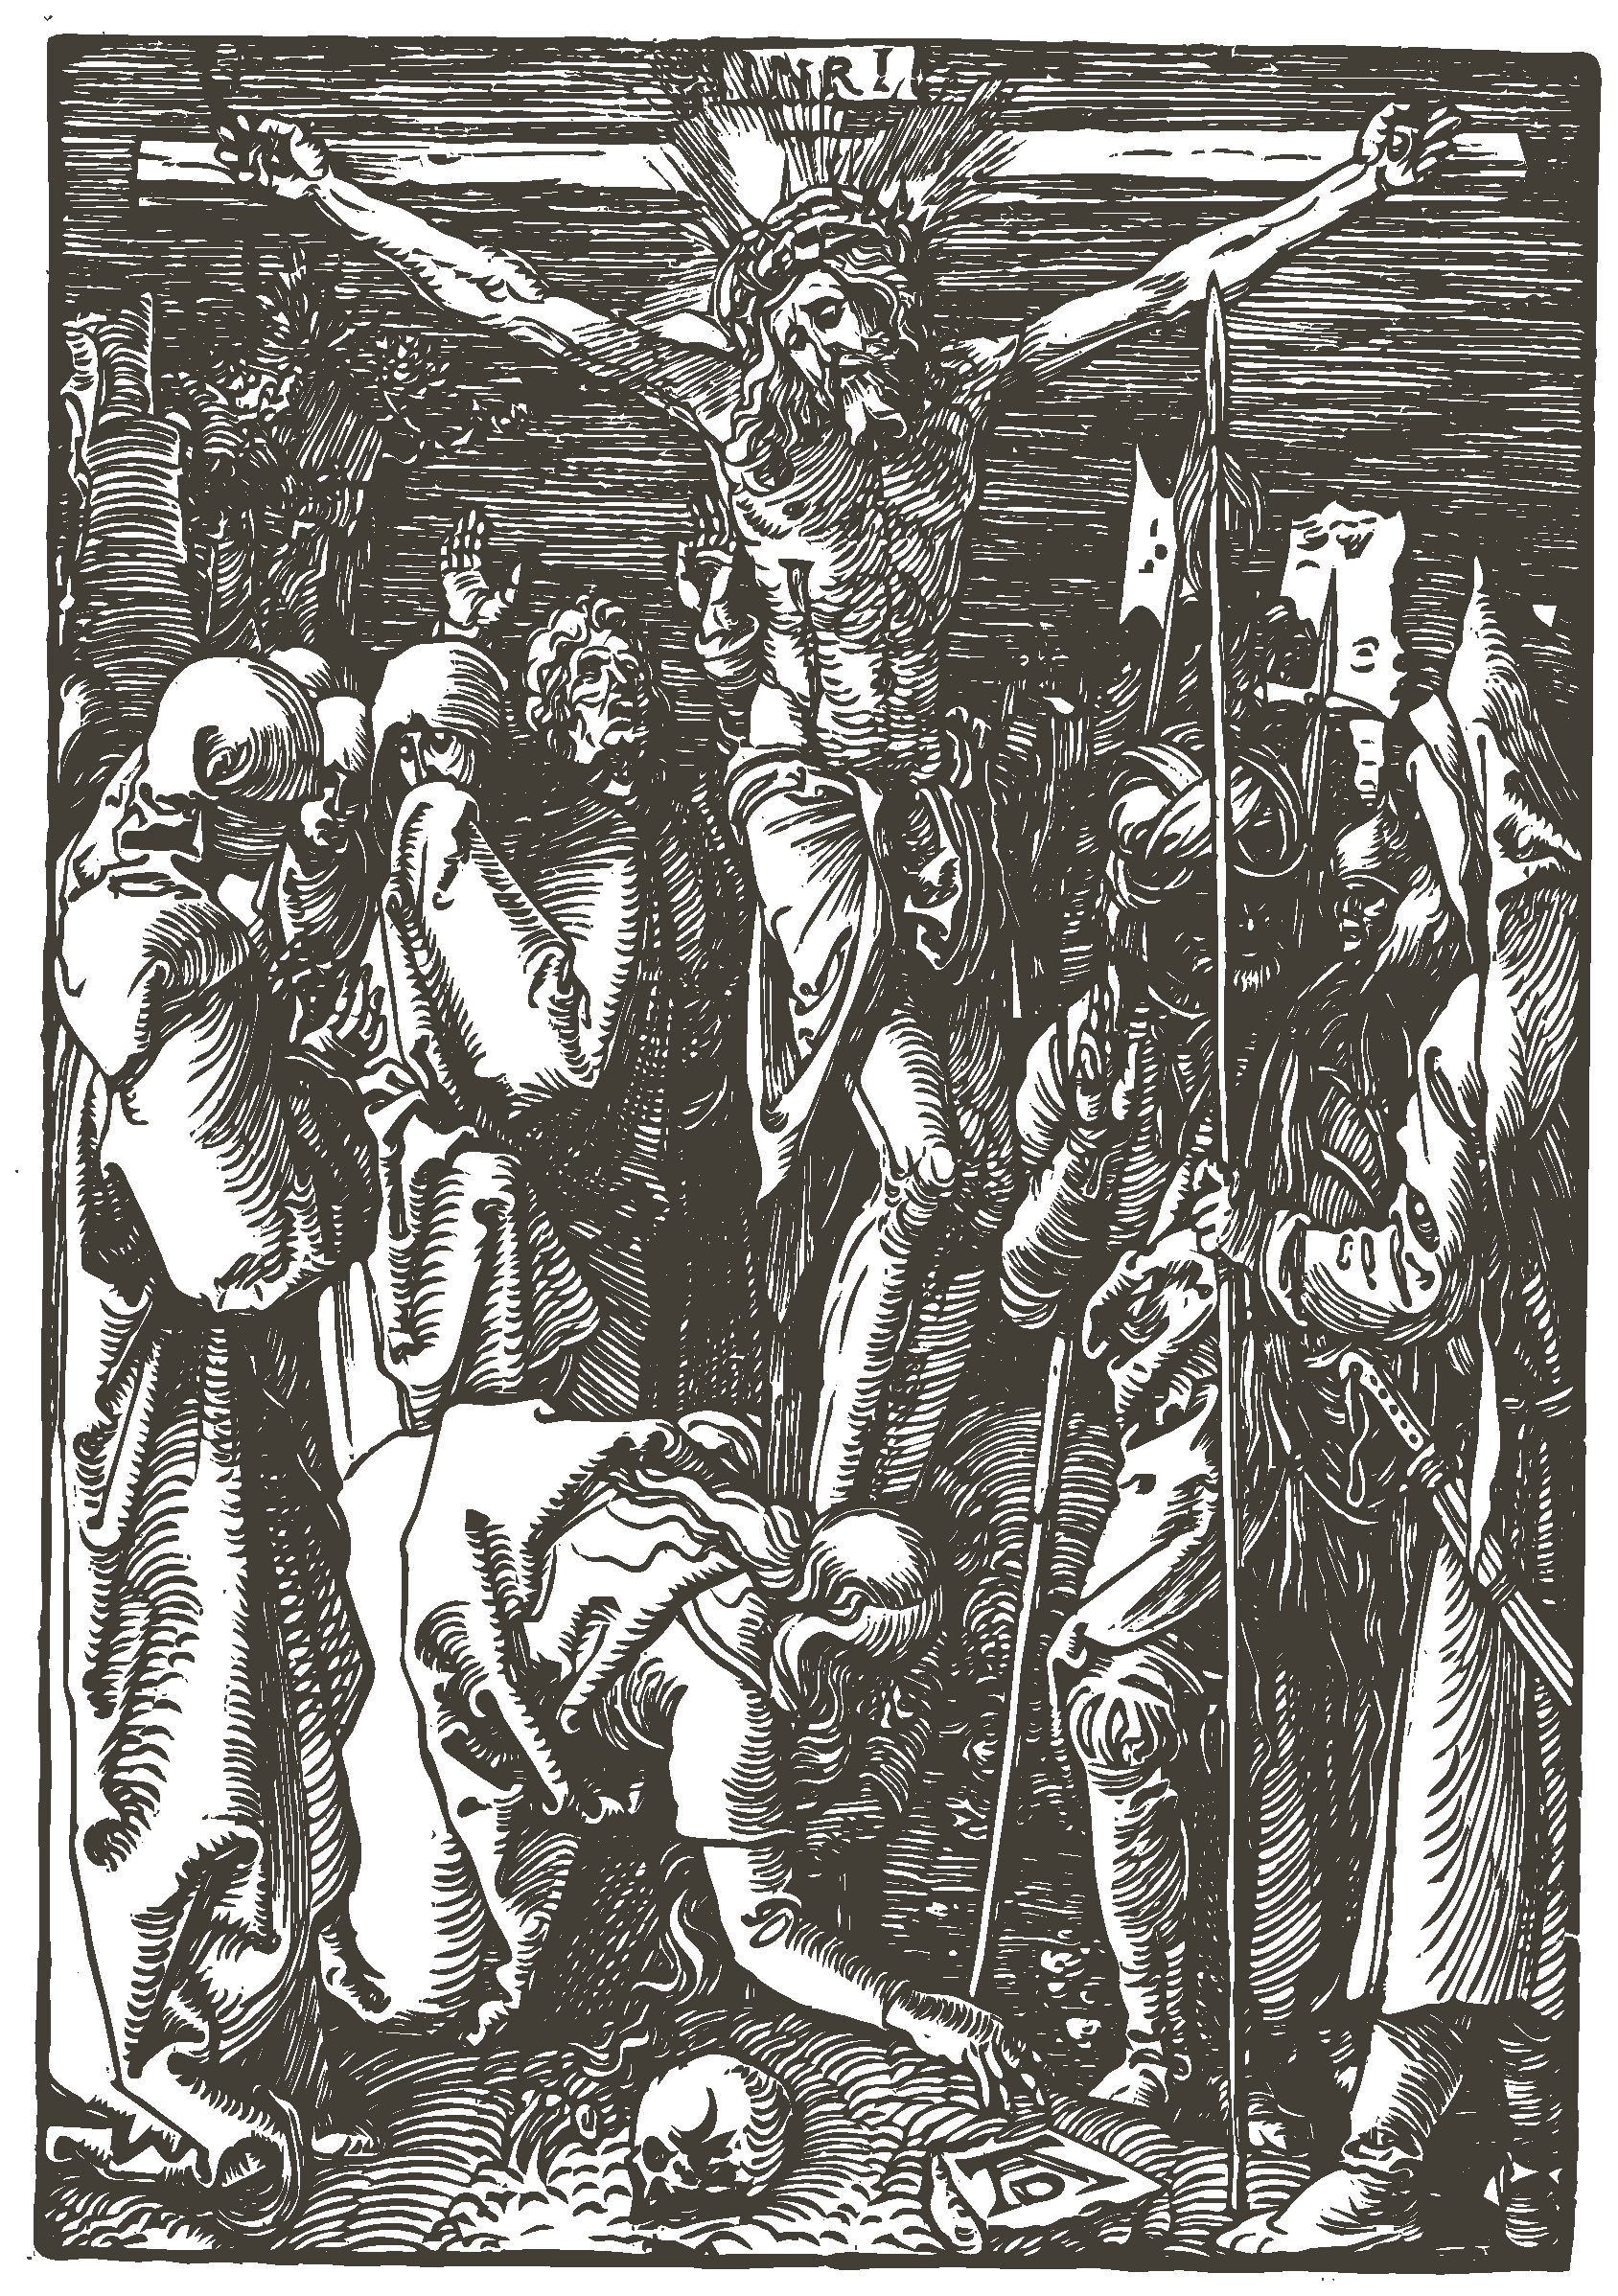
\includegraphics[width=103mm, height=135.497mm]{Mass/Crucifixion.eps}
    \caption{\textsc{\Huge{Holy Mass}}}
\end{figure}
\fancyhead[C]{{\LARGE Holy Mass}}
\fancyhead[RO,LE]{}
\fancyhead[RE,LO]{}
%\fancyhead[RO,LE]{\textit{Liturgy of St. Tikhon}}
%\section{Liturgy of St. Tikhon}\label{tikhon}
\phantomsection
\addcontentsline{toc}{section}{The Holy Communion}
%\begin{rubric}
%If any be an open and notorious evil liver, or have done any wrong to his neighbours by word or deed, so that the Congregation be thereby offended; the Curate, having knowledge thereof, shall call him and advertise him, that in any wise he presume not to come to the Lord’s Table, until he have openly declared himself to have truly repented and amended his former naughty life, that the Congregation may thereby be satisfied, which before were offended; and that he have recompensed the parties, to whom he hath done wrong; or at least declare himself to be in full purpose so to do, as soon as he conveniently may.
%\end{rubric}
%\begin{rubric}
%The same order shall the Curate use with those betwixt whom he perceiveth malice and hatred to reign; not suffering them to be partakers of the Lord's Table, until he know them to be reconciled. And if one of the parties so at variance be content to forgive from the bottom of his heart all that the other hath trespassed against him, and to make amends for that he himself hath offended; and the other party will not be persuaded to a godly unity, but remain still in his frowardness and malice the Minister in that case ought to admit the penitent person to the Holy Communion, and not him that is obstinate.
%\end{rubric}
%\begin{rubric}
%Provided that every Minister so advertising or repelling any, as is specified in the two precedent paragraphs, shall he obliged forthwith to give an account of the same to the Bishop, and therein to obey his order and direction.
%\end{rubric}
%
%
%There is a dispute between the Missals as to where to place the Collect for Purity and the Summary of the Law. The St. Tikhon's Liturgy (as it exists) and the English Missal place it at the Altar, after the Ascent. While this is a fitting place for the Collect, it creates a liturgical novelty for the Summary of the Law. At the Epistle side is offered the prayers to God: the various propers and the sacrifice of the Epistle. In contrast, the Summary of the Law is not directed towards God (who needs no preaching of His own Law) but rather towards the people. Therefore, it is absurd to have the place of sacrifice to God (the Epistle side) be the place of exhortation to the People of God, especially if does not even turn towards the Congregation. There is an example where the Priest does fully turn away from God towards the Congregation: the \emph{Orate Frates}, which occurs in the middle of the Altar. Therefore, to avoid novelties and liturgical inconsistencies, I have placed the Collect and the Summary/Decalogue at the Foot of the Altar, as other Missals have so done (it is appropriate for the Collect, for that is where other collects are read, and it is supremely expedient for an exhortation of the People).
\subsection{Collect for Purity}
\begin{secrubric}
    The Priest, at the Foot of the Altar, saith the Collect for Purity, as followeth, in an audible voice.
\end{secrubric}
\lett{A}{lmighty} God, unto whom all hearts are open, all desires known, and from whom no secrets are hid; Cleanse the thoughts of our hearts by the inspiration of thy Holy Spirit, that we may perfectly love thee, and worthily magnify thy holy Name; through Christ our Lord. \textit{Amen.}
\begin{rubric}
Then shall the Priest, turning to the People, rehearse distinctly---in an audible voice---The Ten Commandments; and the People, still kneeling, shall, after every Commandment, ask God mercy for their transgressions for the time past, and grace to keep the law for the time to come.
\end{rubric}
\begin{rubric}
And \textsc{Note,} that in rehearsing the Ten Commandments, the Priest may omit that part of the Commandment which is inset.
\end{rubric}
\begin{rubric}
	The Decalogue may be omitted. But \textsc{Note,} That when ever it is omitted, the Minister shall say the Summary of the Law, beginning, \blackrubric{Hear what our Lord Jesus Christ saith.}
\end{rubric}

%MANUAL ADJUSTMENT:
\vspace{-2ex}

\subsection{Ten Commandments}

%MANUAL ADJUSTMENT:
\vspace{-0.5ex}

\begin{center}
	\textsc{God spake these words, and said:}
\end{center}

%MANUAL ADJUSTMENT:
\vspace{-0.5ex}

%\begin{multicols}{2}
\par\noindent
    I am the \textsc{Lord} thy God; Thou shalt have none other gods but me.\par
    \textit{Lord, have mercy upon us, and incline our hearts to keep this law.}
    \par\noindent
    Thou shalt not make to thyself any graven image, nor the likeness of any thing that is in heaven above, or in the earth beneath, or in the water under the earth; thou shalt not bow down to them, nor worship them:
    \par\noindent
    \leftskip=2em
	{\small{for I the Lord thy God am a jealous God, and visit the sins of the fathers upon the children, unto the third and fourth generation of them that hate me; and show mercy unto thousands in them that love me and keep my commandments.}}
	\par
	\leftskip=0cm
    \textit{Lord, have mercy upon us, and incline our hearts to keep this law.}
    \par\noindent
    Thou shalt not take the Name of the Lord thy God in vain;
    \par\noindent
    \leftskip=2em
	{\small{for the Lord will not hold him guiltless, that taketh his Name in vain.}}
	\par
	\leftskip=0em
    \textit{Lord, have mercy upon us, and incline our hearts to keep this law.}
    \par\noindent
    Remember that thou keep holy the Sabbath-day.
    \par\noindent
    \leftskip=2em
	{\small{Six days shalt thou labour, and do all that thou hast to do; but the seventh day is the Sabbath of the Lord thy God. In it thou shalt do no manner of work; thou, and thy son, and thy daughter, thy man-servant, and thy maid-servant, thy cattle, and the stranger that is within thy gates. For in six days the Lord made heaven and earth, the sea, and all that in them is, and rested the seventh day: wherefore the Lord blessed the seventh day, and hallowed it.}}
	\par
	\leftskip=0em
    \textit{Lord, have mercy upon us, and incline our hearts to keep this law.}
    \par\noindent
    Honour thy father and thy mother;
    \par\noindent
    \leftskip=2em
	{\small{that thy days may be long in the land which the Lord thy God giveth thee.}}
	\par
	\leftskip=0em
    \textit{Lord, have mercy upon us, and incline our hearts to keep this law.}
    \par\noindent
    Thou shalt do no murder.\par
    \textit{Lord, have mercy upon us, and incline our hearts to keep this law.}
    \par\noindent
    Thou shalt not commit adultery.\par
    \textit{Lord, have mercy upon us, and incline our hearts to keep this law.}
\par\noindent
    Thou shalt not steal.\par
    \textit{Lord, have mercy upon us, and incline our hearts to keep this law.}
\par\noindent
    Thou shalt not bear false witness against thy neighbour.\par
    \textit{Lord, have mercy upon us, and incline our hearts to keep this law.}
    \par\noindent
    Thou shalt not covet.
    \par\noindent
    \leftskip=2em
	{\small{thy neighbour's house, thou shalt not covet thy neighbour's wife, nor his servant, nor his maid, nor his ox, nor his ass, nor any thing that is his.}}
	\par
	\leftskip=0em
	\textit{Lord, have mercy upon us, and write all these thy laws in our hearts, we beseech thee.}
	
%	\end{multicols}
\begin{rubric}
	Then may the Priest say the Summary of the Law, as followeth, in an audible voice.
\end{rubric}
\subsection{Summary of the Law}
\begin{center}
	{\textsc{Hear what our Lord Jesus Christ saith.}}
\end{center}

\lett{T}{hou} shalt love the Lord thy God with all thy heart, and with all thy soul, and with all thy mind. This is the first and great commandment. And the second is like unto it; Thou shalt love thy neighbour as thyself. On these two commandments hang all the Law and the Prophets.

\subsection{Ascending the Altar}

\begin{rubric}
    Then shall the Priest turn towards the Altar and ascend, saying secretly,%\blackrubric{Take away}.
\end{rubric}
\lett{T}{ake} away from us, we beseech thee, O Lord, our iniquities: that we may be worthy to enter with pure minds into the Holy of holies. Through Christ, our Lord. Amen.
\begin{rubric}
    Then, with hands joined upon the Altar, the Priest saith, bowing (kissing the Altar at the middle),% \blackrubric{We pray thee}.
\end{rubric}
\lett{W}{e} pray thee, O Lord, by the merits of thy Saints, * whose relics are here, and of all the Saints: that thou wouldest vouchsafe to pardon all my sins. Amen.
\begin{rubric}
    At a solemn Mass, the Celebrant, before reading the Introit, shall bless the incense saying: \blackrubric{Be thou bles {\ding{64}} sed by him in whose honour thou shalt be burnt. Amen.}
\end{rubric}
\begin{rubric}
	Receiving the thurible from the Deacon, he censeth the Altar, saying nothing. Then the Deacon taketh the thurible from the Celebrant and censeth him only.
\end{rubric}
\begin{rubric}
%Added clarity that the Priest should be in the middle of the Altar for the Kyrie.
    Then shall the Priest move to the Epistle side and, signing himself with the sign of the Cross, begin the Introit: which finished, at the middle of the Altar, with joined hands, he saith alternately with the Ministers the \blackrubric{Kyrie,}
\end{rubric}

%MANUAL ADJUSTMENT:
\vspace{-0.75\baselineskip}

\subsection{Kyrie}
\elcoldent{℣. Lord, have mercy upon us.}{℣. Kyrie, eléison.}
\elcoldent{℟. Lord, have mercy upon us.}{℟. Kyrie, eléison.}
\elcoldent{℣. Lord, have mercy upon us.}{℣. Kyrie, eléison.}
\elcoldent{℟. Christ, have mercy upon us.}{℟. Christe, eléison.}
\elcoldent{℣. Christ, have mercy upon us.}{℣. Christe, eléison.}
\elcoldent{℟. Christ, have mercy upon us.}{℟. Christe, eléison.}
\elcoldent{℣. Lord, have mercy upon us.}{℣. Kyrie, eléison.}
\elcoldent{℟. Lord, have mercy upon us.}{℟. Kyrie, eléison.}
\elcoldent{℣. Lord, have mercy upon us.}{℣. Kyrie, eléison.}

%MANUAL ADJUSTMENT:
\vspace{-0.15\baselineskip}

\subsection{Gloria in excelsis}

%MANUAL ADJUSTMENT:
\vspace{-0.1\baselineskip}

\begin{rubric}
    Then the Priest shall, at the middle of the Altar, extend and join his hands and---bowing his head slightly---say, if it is to be said,
\end{rubric}
\elcol{\lett{G}{lory} be to God on high, and on earth peace, good will towards men. We praise thee, we bless thee, we worship thee,\margcolrub{1}{Bow head.} we glorify thee, we give thanks\margcolrub{2}{Bow head.} to thee for thy great glory, O Lord God, heavenly King, God the Father Almighty.\par
	O Lord, the only-begotten Son, Jesus Christ; O Lord God, Lamb of God, Son of the Father, that takest away the sins of the world, have mercy upon us. Thou that takest away the sins of the world, receive our prayer.\margcolrub{3}{Bow head.} Thou that sittest at the right hand of God the Father, have mercy upon us.\par
	For thou only art holy; thou only art the Lord; thou only, O Christ, with the Holy Ghost, {\ding{64}} art most high in the glory of God the Father. Amen.}
    {\lett{G}{l\smash{ó}ria} in excélsis Deo. Et in terra pax homínibus bon{\ae} voluntátis. Laudámus te. Benedícimus te. Adorámus te.\marglatincolrub{1}{Bow head.} Glorificámus te. Grátias ágimus tibi\marglatincolrub{2}{Bow head.} propter magnam glóriam tuam. Dómine Deus, Rex c{\ae}léstis, Deus Pater omnípotens.\par
    Dómine Fili unigénite, Jesu Christe. Dómine Deus, Agnus Dei, Fílius Patris. Qui tollis peccáta mundi, miserére nobis. Qui tollis peccáta mundi, súscipe deprecatiónem nostram.\marglatincolrub{3}{Bow head.} Qui sedes ad déxteram Patris, miserére nobis.\par
    Quóniam tu solus Sanctus. Tu solus Dóminus. Tu solus Altíssimus, Jesu Christe. Cum Sancto Spíritu {\ding{64}} in glória Dei Patris. Amen.}

\begin{rubric}
    Then shall the Priest kiss the Altar in the middle, turn to the People, extend his hands, and say,
\end{rubric}

\elcol{℣. The Lord be with you.}{℣. Dóminus vobíscum.}
\elcol{℟. And with thy spirit.}{℟. Et cum spíritu tuo.}
\elcol{℣. Let us pray.}{℣. Orémus.}

%MANUAL ADJUSTMENT:
\vspace{-2ex}

\subsection{Collect}
\begin{rubric}
	Then shall the Priest move to the Epistle corner of the Altar and pray the Collect(s) of the Day.
\end{rubric}

%MANUAL ADJUSTMENT:
\vspace{-4ex}

\subsection{Epistle}
\begin{rubric}
	The Epistle for the Day shall then be read by the Subdeacon, first saying, \blackrubric{The Epistle is written in the \emph{--} Chapter of \emph{--}, beginning at the \emph{--} Verse.}
\end{rubric}
\begin{rubric}
	The Epistle ended, he shall say, \blackrubric{Here endeth the Epistle,} the people responding, \blackrubric{Thanks be to God.}
\end{rubric}
\begin{rubric}
    The Gradual and Alleluia (or Tract) and (if provided) Sequence is here chanted by the Choir.
\end{rubric}

%MANUAL ADJUSTMENT:
\vspace{-4ex}

\subsection{Gospel}
%\begin{multicols}{2}
\begin{rubric}
    These being ended, if it be a Solemn Mass, the Deacon shall then place the book of the Gospels on the middle of the Altar, and the Celebrant shall bless the incense with the \blackrubric{Be thou blessed,} as above.
\end{rubric}
\begin{rubric}
	Then shall the Deacon kneeling before the Altar (or the Priest only bowing in the midst of the Altar) say with joined hands,% the \blackrubric{Cleanse my heart} continuing to the \blackrubric{Bid, sir}, with the priest saying \blackrubric{The Lord be in thy}.
\end{rubric}

\lett{C}{leanse} my heart and my lips, O almighty God, who didst cleanse the lips of the prophet Isaiah with a live coal: so of thy gracious mercy vouchsafe to cleanse me, that I may worthily proclaim thy holy Gospel. Through Christ, our Lord. Amen.

\begin{paracol}{2}

\sloppy

\begin{inhead}
	Deacon
\end{inhead}
\par\noindent
	\emph{Deacon.} Bid, sir, a blessing.\par\noindent
	\emph{Priest.} The Lord be in thy heart and on thy lips: that thou mayest worthily and fitly proclaim his Gospel: In the name of the Father, and of the Son, {\ding{64}} and of the Holy Ghost. Amen.

\switchcolumn

\begin{inhead}
	Priest
\end{inhead}
	\par\noindent
	\emph{Priest.} Bid, Lord, a blessing.\par\noindent
	\emph{Priest.} The Lord be in my heart and on my lips: that I may worthily and fitly proclaim his Gospel. 
	
	\fussy
	
\end{paracol}


\begin{rubric}
    Having received the blessing, the Deacon kisseth the hand of the Celebrant. And going with the other Ministers, with the incense and the lights, to the place of the Gospel, he standeth with joined hands.%, saying what is below.
\end{rubric}
%Unnecessary rubric:
%\begin{rubric}
%    If, however, the Priest celebrate without Deacon and Subdeacon, when the book has been carried to the other corner of the Altar, he boweth in the middle, and with joined hands, saith the \blackrubric{Cleanse my heart} and the \blackrubric{Bid, Lord} and \blackrubric{The Lord be in my}.
%\end{rubric}

%\end{multicols}
\begin{rubric}
	Then, the People standing, the Deacon, turning to the Book, saith with joined hands,
\end{rubric}
\elcol{℣. The Lord be with you.}{℣. Dóminus vobíscum.}
\elcol{℟. And with thy spirit.}{℟. Et cum spíritu tuo.}
\elcol{℣. The Beginning (or, Continuation) {\ding{66}} of the Holy Gospel according to \textit{N.}

℟. Glory be to thee, O Lord.}{℣. Inítium (vel, Sequéntia) {\ding{66}} sancti Evangélii secúndum \textit{N.}

℟. Glória tibi, Dómine.}

\begin{rubric}
    Then shall the Deacon sign the book with the thumb of his right hand at the beginning of the Gospel text which he is to read, then himself on the forehead, the mouth, and the breast: and while the Ministers respond, he censeth the book thrice, then readeth the Gospel with joined hands.
\end{rubric}
\begin{rubric}
    At the end of the Gospel, the Ministers respond,
\end{rubric}
\elcol{℟. Praise be to thee, O Christ.}{℟. Laus tibi, Christe.}
\begin{rubric}
    Then shall the Subdeacon carry the book to the Priest, who kisseth the Gospel text, saying: \blackrubric{Through the words of the Gospel may our sins be blotted out.} Then the Priest is censed by the Deacon.\par
    \textsc{Note,} In Masses of the Dead, \blackrubric{Cleanse} is said, but a blessing is not asked, lights are not carried, and the Celebrant doth not kiss the book.
\end{rubric}
\begin{rubric}
    Then, in the middle of the Altar, extending, raising, and joining his hands, the Priest shall say, if it is to be said, \blackrubric{I believe in one God,} proceeding with joined hands.
\end{rubric}
\subsection{Nicene Creed}\label{NiceneCreed}
\elcol{\lett{I}{believe} in one God\margcolrub{4}{Bow head to Cross.} the Father Almighty, Maker of heaven and earth, And of all things visible and invisible:\par
    And in one Lord Jesus Christ,\margcolrub{5}{Bow head to Cross.} the only-begotten Son of God; Begotten of his Father before all worlds, God of God, Light of Light, Very God of very God; Begotten, not made; Being of one substance with the Father; By whom all things were made: Who for us men and for our salvation came down from heaven, \inrub{Everyone genuflects.} And was incarnate by the Holy Ghost of the Virgin Mary, And was made man: \inrub{Everyone rises.} And was crucified also for us under Pontius Pilate; He suffered and was buried: And the third day he rose again according to the Scriptures: And ascended into heaven, And sitteth on the right hand of the Father: And he shall come again, with glory, to judge both the quick and the dead; Whose kingdom shall have no end.\par
    And I believe in the Holy Ghost, The Lord, and Giver of Life, Who proceedeth from the Father; Who with the Father and the Son together is worshiped\margcolrub{6}{Bow head to Cross.} and glorified; Who spake by the Prophets: And I believe one, holy, catholic, and apostolic Church: I acknowledge one Baptism for the remission of sins: And I look for the Resurrection of the dead: {\ding{64}} And the Life of the world to come. Amen.}
    {\lett{C}{redo} in unum Deum,\marglatincolrub{4}{Bow head to Cross.} Patrem omnipoténtem, factórem c{\ae}li et terr{\ae}, visibílium ómnium et invisibílium.\par
    Et in unum Dóminum Jesum Christum,\marglatincolrub{5}{Bow head to Cross.} Fílium Dei unigénitum. Et ex Patre natum ante ómnia sǽcula. Deum de Deo, lumen de lúmine, Deum verum de Deo vero. Génitum, non factum, consubstantiálem Patri: per quem ómnia facta sunt. Qui propter nos hómines et propter nostram salútem descéndit de c{\ae}lis. \inrub{Everyone genuflects.} Et incarnátus est de Spíritu Sancto ex María Vírgine: Et homo factus est. \inrub{Everyone rises.} Crucifíxus étiam pro nobis: sub Póntio Piláto passus, et sepúltus est. Et resurréxit tértia die, secúndum Scriptúras. Et ascéndit in c{\ae}lum: sedet ad déxteram Patris. Et íterum ventúrus est cum glória judicáre vivos et mórtuos: cujus regni non erit finis.\par
    Et in Spíritum Sanctum, Dóminum et vivificántem: qui ex Patre procédit. Qui cum Patre et Fílio simul adorátur\marglatincolrub{6}{Bow head to Cross.} et conglorificátur: qui locútus est per Prophétas. Et unam sanctam cathólicam et apostólicam Ecclésiam. Confíteor unum baptísma in remissiónem peccatórum. Et exspécto resurrectiónem mortuórum. {\ding{64}} Et vitam ventúri s{\ae}culi. Amen.}
\begin{rubric}
Then shall be declared unto the People what Holy-days, or Fasting-days, are in the week following to be observed; and (if occasion be) shall Notice be given of the Communion, and of the Banns of Matrimony, and other matters to be published.
\end{rubric}

\begin{rubric}
Here, or immediately after the Creed, may be said the Bidding Prayer, or other authorized Prayers and intercessions.
\end{rubric}

\begin{rubric}
	Then followeth the Sermon.
\end{rubric}

\begin{rubric}
    Then shall the Priest ascend the Altar, kiss it, turn towards the People, and say,
\end{rubric}
\elcol{℣. The Lord be with you.}{℣. Dóminus vobíscum.}
\elcol{℟. And with thy spirit.}{℟. Et cum spíritu tuo.}
\elcol{℣. Let us pray.}{℣. Orémus.}

%MANUAL ADJUSTMENT:
\clearpage

\subsection{Censing the Gifts}
	
\begin{rubric}
	The following is made in the form of a Cross.
\end{rubric}

	\begin{figure}[H]
		\centering
		
\includegraphics[width=65mm,height=64.316mm]{Mass/CensingGifts.eps}
	\end{figure}
	
	\vfill
	
	\begin{rubric}
	The following is made in the form of a circle.
	\end{rubric}
	
	\begin{figure}[H]
		\centering
		
\includegraphics[width=65mm,height=65.655mm]{Mass/CensingChalice.eps}
	\end{figure}
	
\thispagestyle{empty}
\clearpage

\subsection{Censing the High Altar}

\begin{figure}[H]
    \centering
    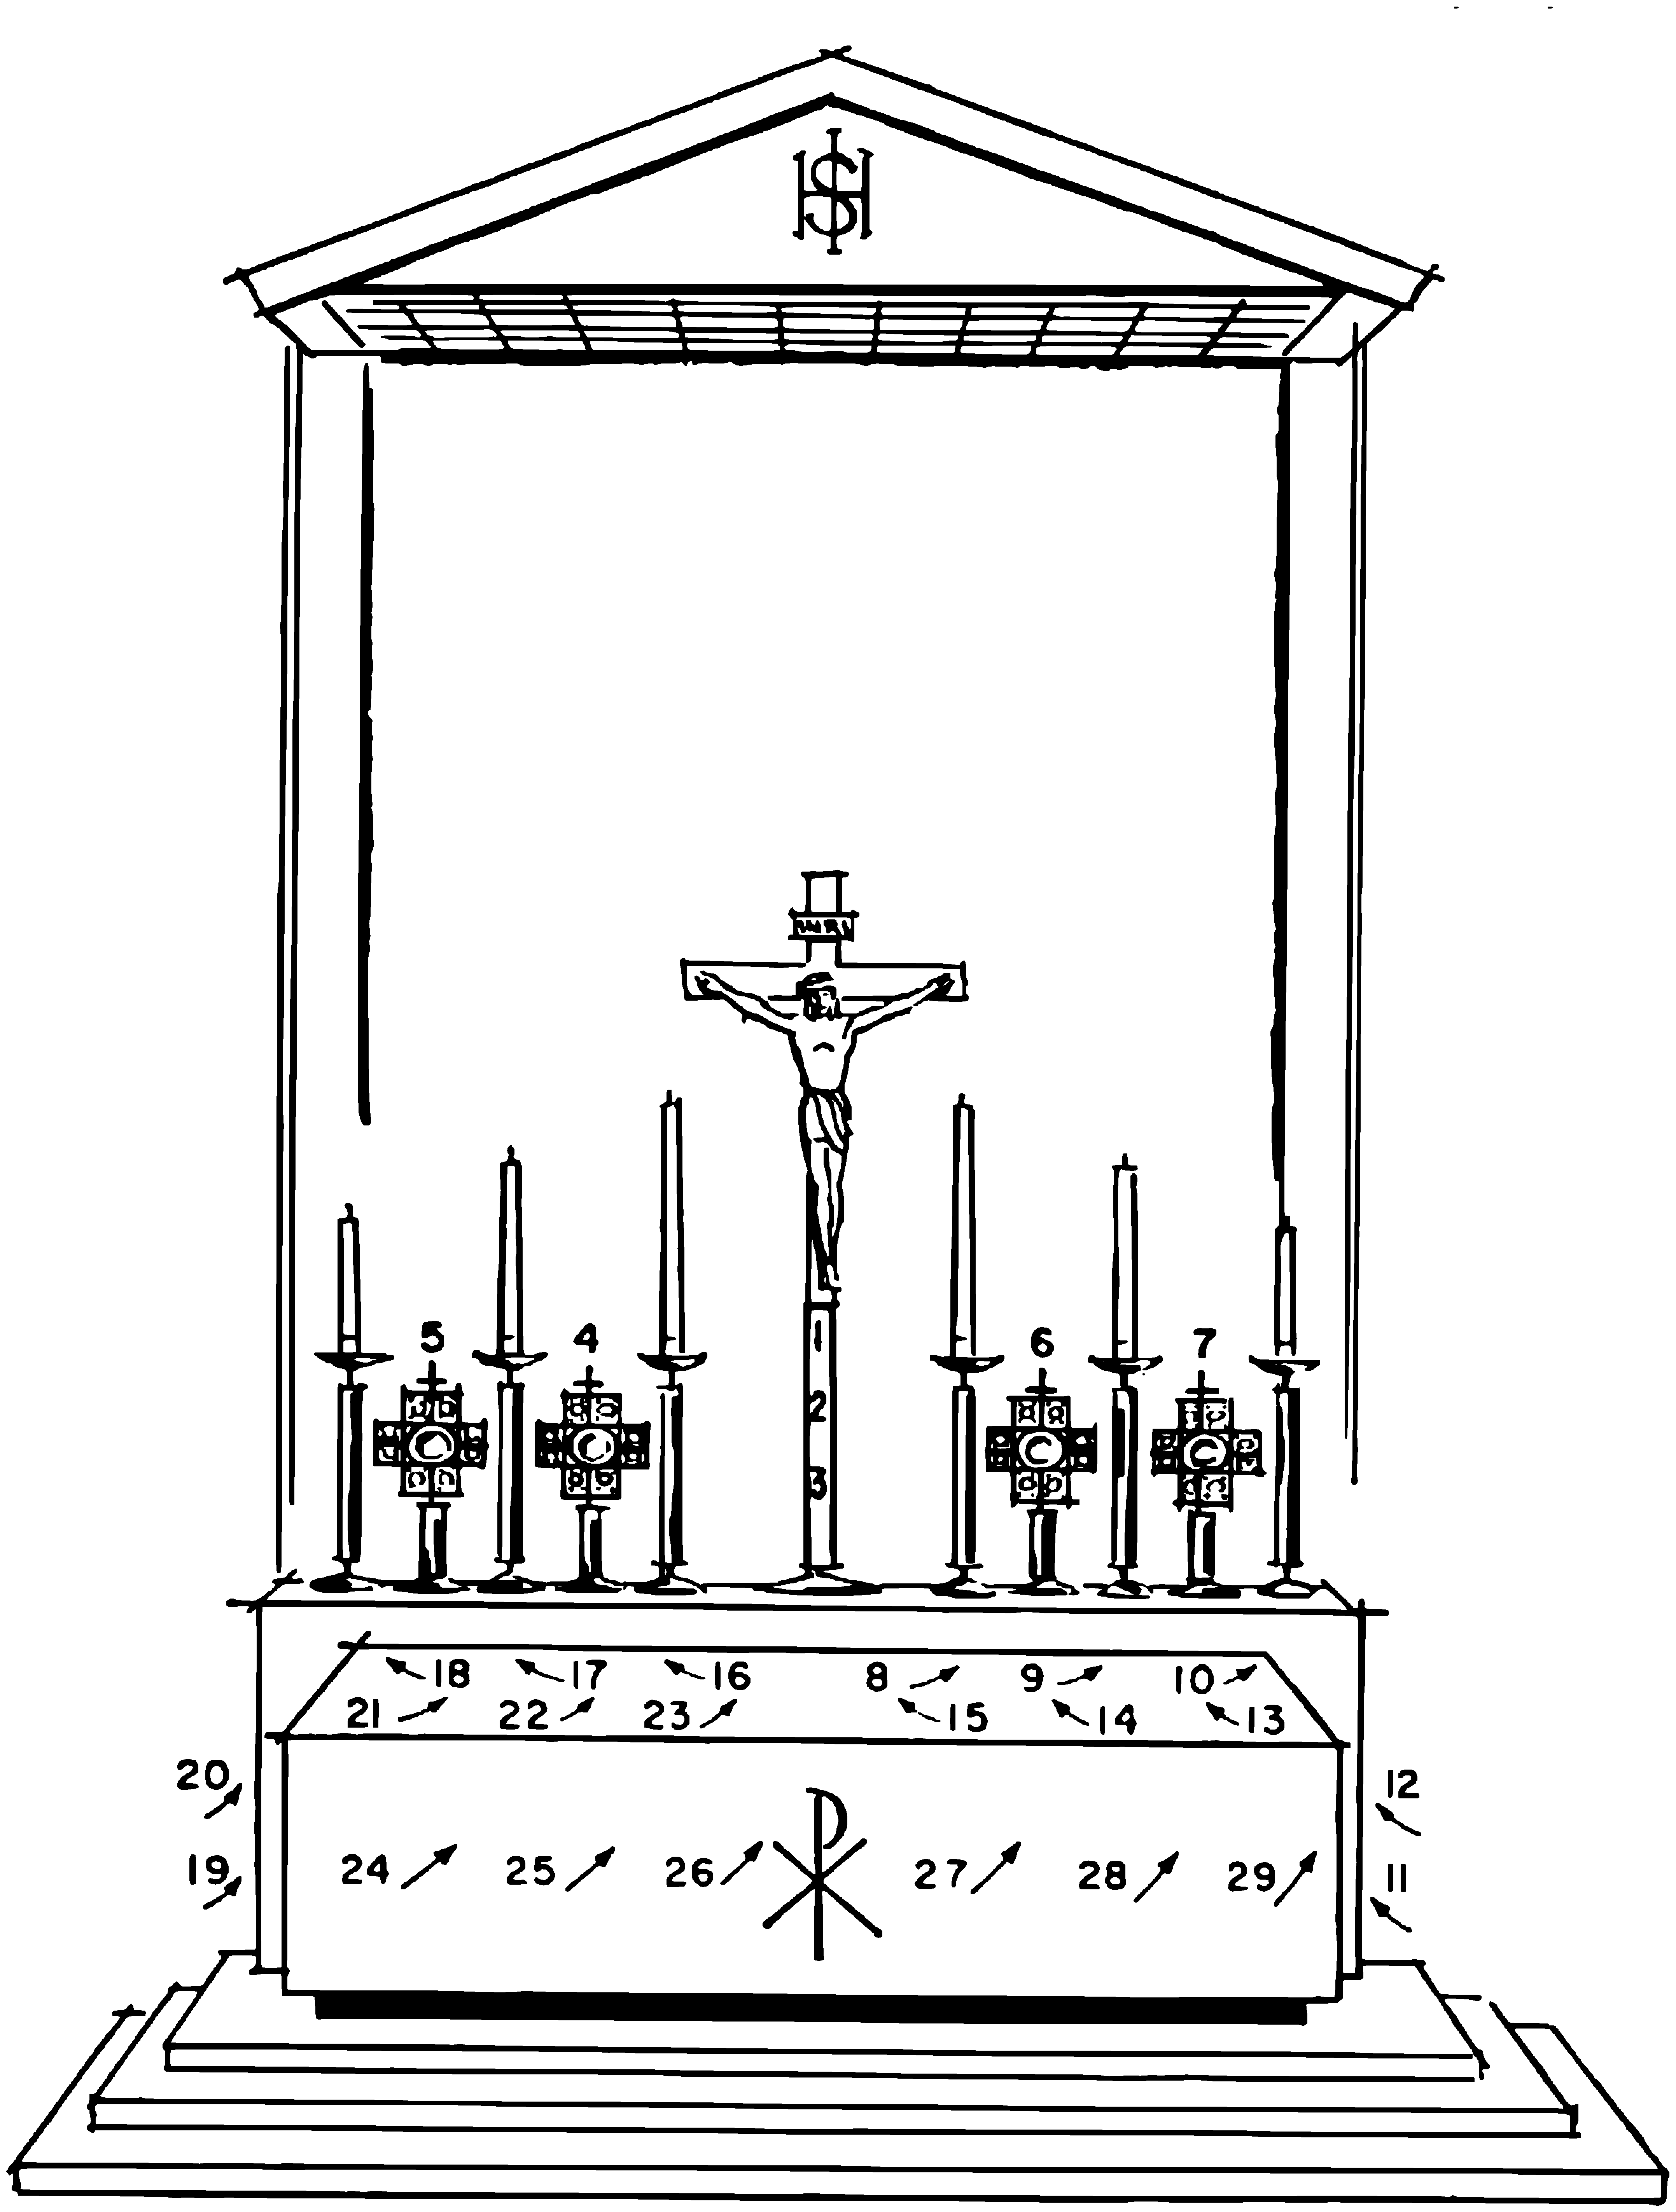
\includegraphics[width=103mm,height=136.234mm]{Mass/CensingAltar.eps}
\end{figure}

\thispagestyle{empty}
\clearpage

\subsection{Censing a Free-Standing Altar}

\begin{figure}[H]
    \centering
    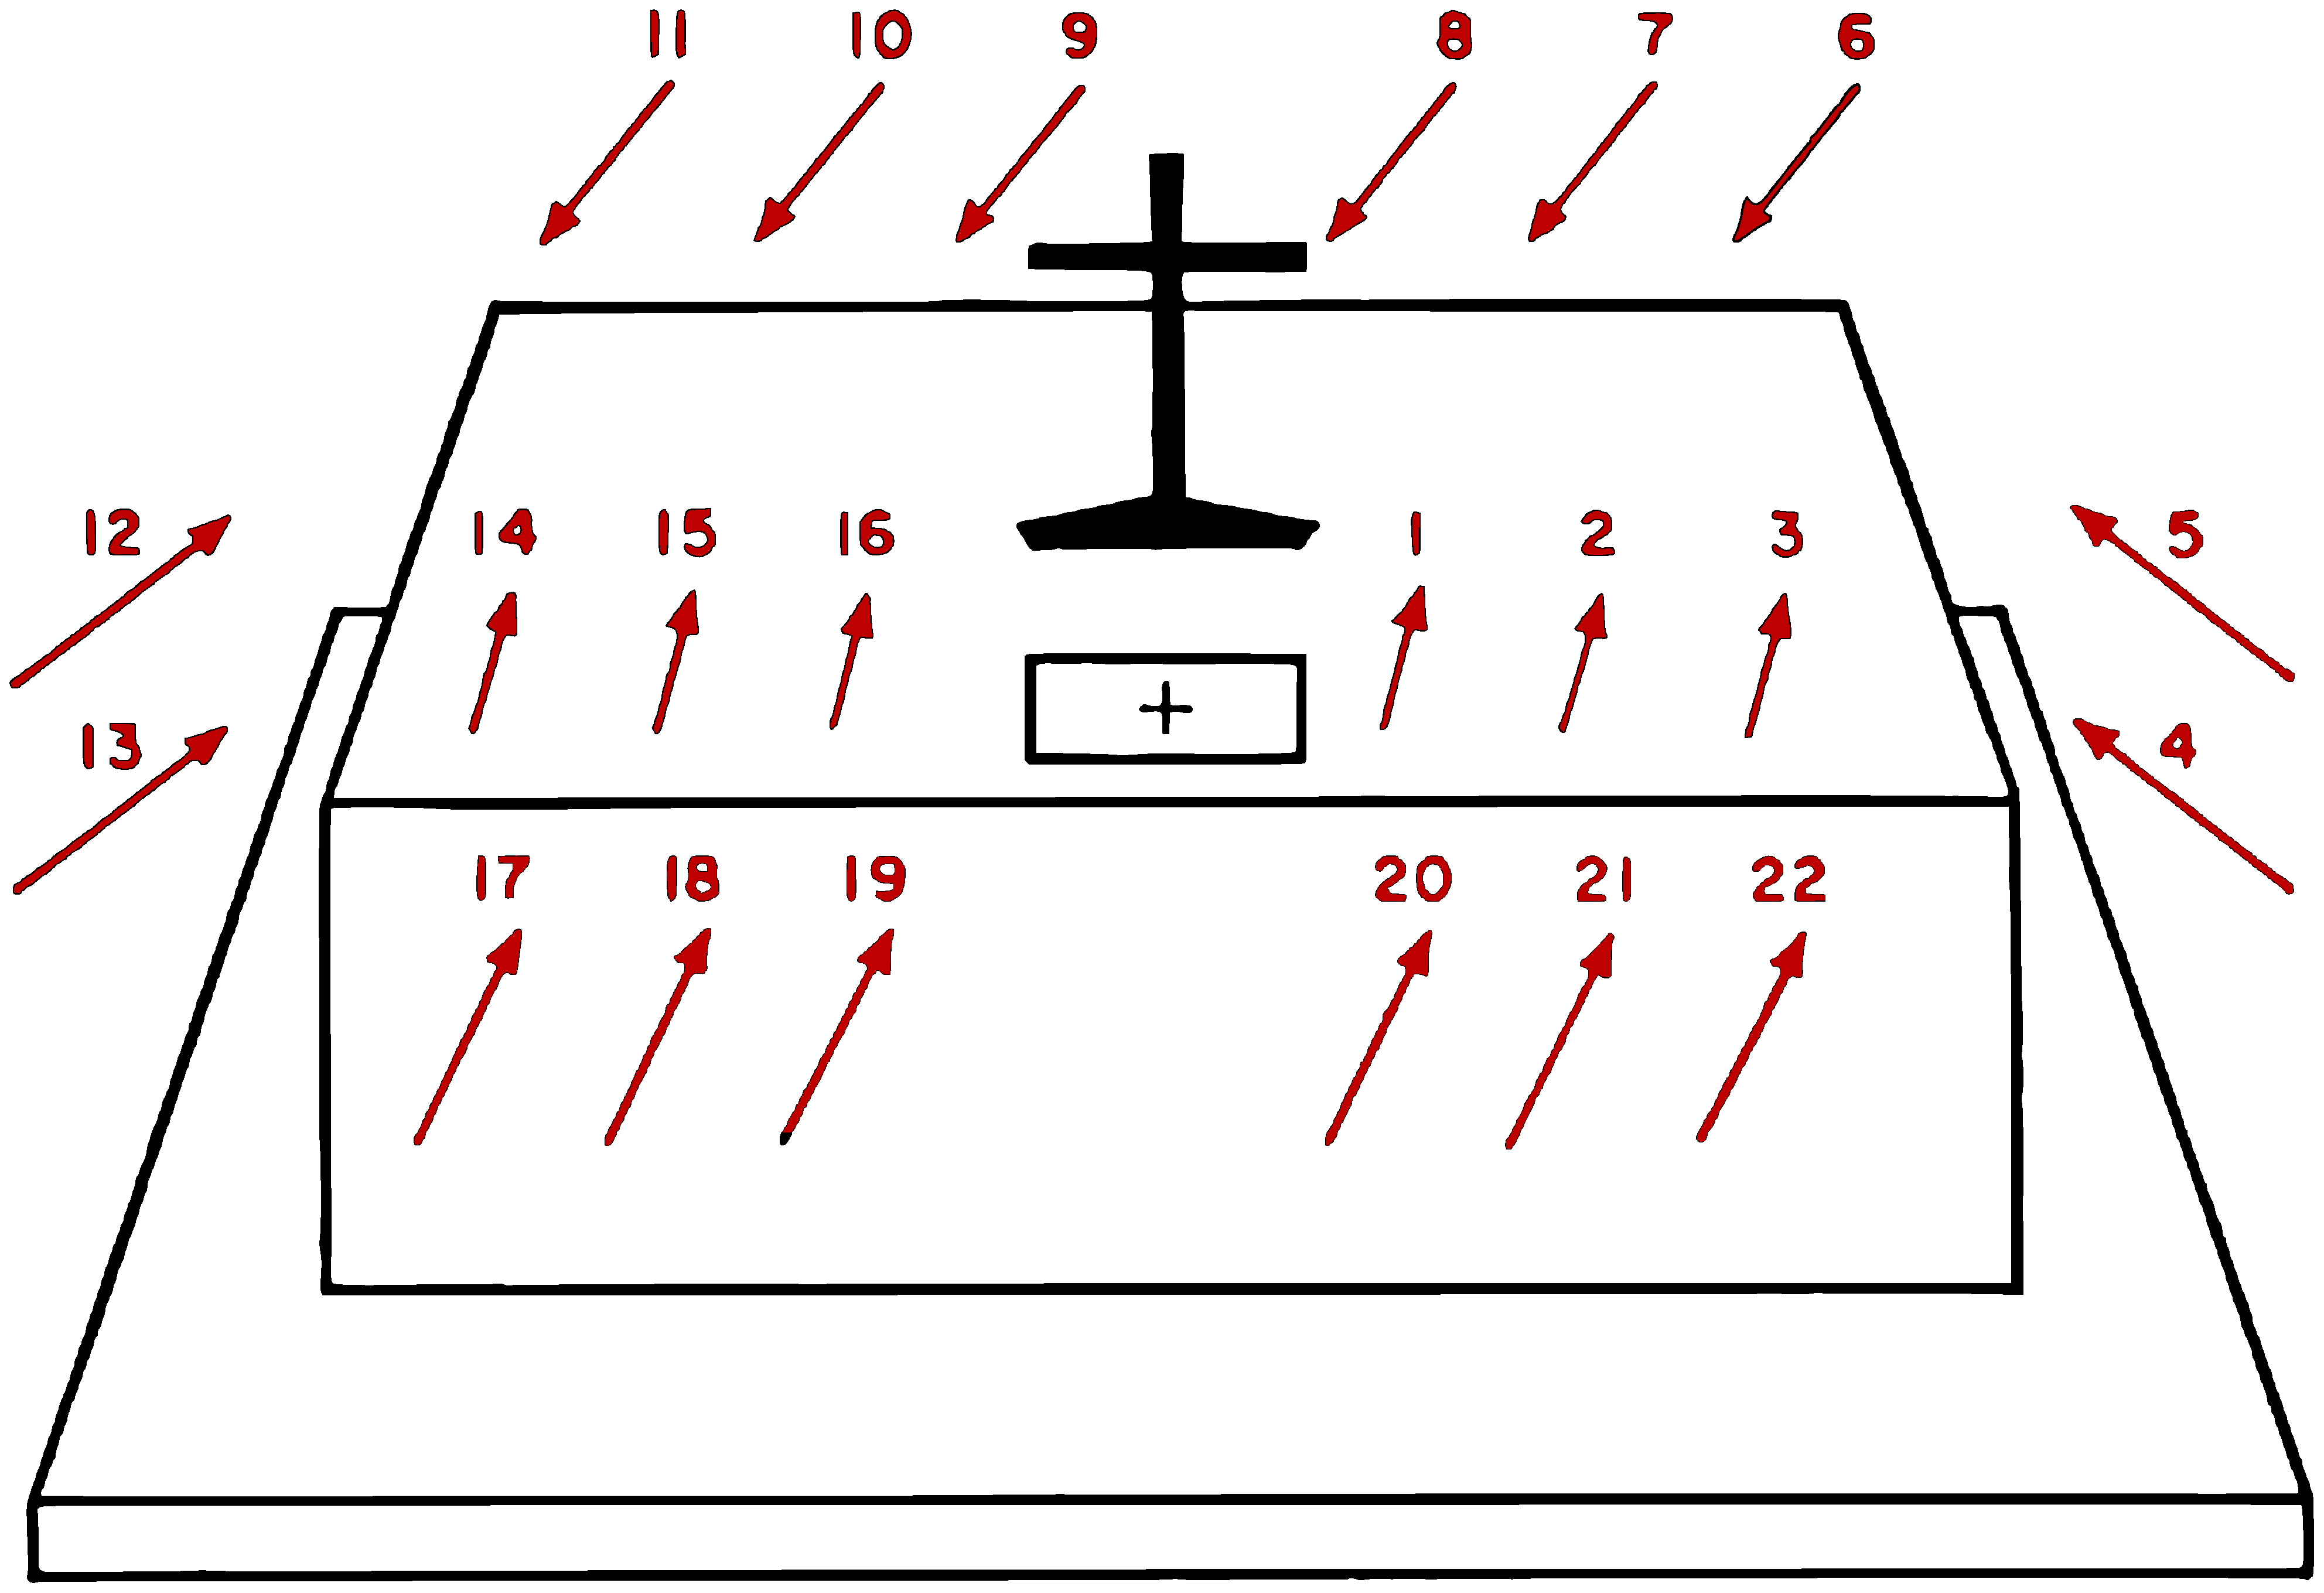
\includegraphics[width=103mm,height=70.303mm]{Mass/CensingFreestandingAltar.eps}
\end{figure}

\thispagestyle{empty}
\clearpage

\subsection{Offertory}

%\begin{multicols}{2}    
\begin{rubric}
    The Priest then saith the Offertory Verse.
\end{rubric}

\begin{rubric}
	\textsc{Note,} At High Mass, a hymn may be sung while the Priest prepareth the Oblations in the Offertory, and while the Collection is taken, if there be one.
\end{rubric}

\subsubsection{Offering the Bread}
\begin{secrubric}
    Then shall the Deacon present the Paten with the Bread to the Celebrant, which he then offereth, saying,%: \blackrubric{Receive, O holy Father}.
\end{secrubric}
\lett{R}{eceive,} O holy Father, almighty everlasting God, this spotless host, which I, thine unworthy servant, offer unto thee, my living and true God, for my numberless sins, offences, and negligences, and for all who stand around, as also for all faithful Christians, both living and departed: that to me and to them it may avail for salvation unto life eternal. Amen.
\begin{rubric} 
    Then, making a cross with the same Paten, he shall place the Bread upon the Corporal (or the Paten with the Bread upon the Corporal).
\end{rubric}

\subsubsection{Offering the Wine}
\begin{secrubric}
	Then the Deacon shall minister the Wine, and the Subdeacon the Water into the Cup. The Priest (blessing with the sign of the Cross the Water to be mixed in the Cup, unless it be a Requiem Mass) shall say,%: \blackrubric{O God, who didst wonderfully}.
\end{secrubric}
\lett{O}{God,} who didst wonderfully create, and yet more wonderfully renew the dignity of man's nature: grant that by the mystery of this water and wine we may be made partakers of his divinity, who vouchsafed to share our humanity, Jesus Christ thy Son our Lord: Who liveth and reigneth with thee in the unity of the Holy Ghost, God: throughout all ages world without end. Amen.
\begin{rubric}
    Then shall the Priest receive the Cup and offer it, saying,% \blackrubric{We offer unto thee}.
\end{rubric}
\lett{W}{e} offer unto thee, O Lord, the cup of salvation, humbly beseeching thy mercy: that in the sight of thy divine majesty it may ascend as a sweet-smelling savour for our salvation, and for that of the whole world. Amen.

%MANUAL ADJUSTMENT:
\clearpage
\subsubsection{Offering the Gifts}
\begin{secrubric}
    Then shall he make the sign of the Cross with the Cup, place it upon the Corporal, and cover it with the Pall. Then, with hands joined upon the Altar, he saith, bowing slightly,% \blackrubric{In a humble spirit}.
\end{secrubric}
\lett{I}{n} a humble spirit, and with a contrite heart, may we be accepted of thee, O Lord: and so let our sacrifice be offered in thy sight this day, that it may be pleasing unto thee, O Lord God.
\begin{rubric}
    Then shall the Priest---standing upright---extend his hands, raise them, and join them; and lifting his eyes to heaven and lowering them immediately, he saith,% \blackrubric{Come, O Sanctifier}.
\end{rubric}
\lett{C}{ome,} O Sanctifier almighty, everlasting God, and bl {\ding{64}} ess this sacrifice, prepared for thy holy Name.

\lettspace

\subsubsection{Censing the Altar}
\begin{secrubric}
    If he be celebrating solemnly, the Priest blesseth incense, saying,% \blackrubric{Through the intercession of blessed Michael the Archangel standing at the right hand of the altar of incense, and of all his elect, may the Lord vouchsafe to bl {\ding{64}} ess this incense, and receive it for a sweet-smelling savour. Through Christ, our Lord. Amen.}.
\end{secrubric}
\lett{T}{hrough} the intercession of blessed Michael the Archangel standing at the right hand of the altar of incense, and of all his elect, may the Lord vouchsafe to bl {\ding{64}} ess this incense, and receive it for a sweet-smelling savour. Through Christ, our Lord. Amen.
\begin{rubric}
    Receiving the Thurible from the Deacon, he censeth the Oblations, in the manner prescribed in the traditional manner, saying,%: \blackrubric{May this incense which thou hast blessed, ascend unto thee, O Lord: and let thy mercy descend upon us.}.\par
\end{rubric}
\lett{M}{ay} this incense which thou hast blessed, ascend unto thee, O Lord: and let thy mercy descend upon us.

\lettspace

\begin{rubric}
    Then the Priest censeth the Altar, saying,%: \blackrubric{Let my prayer}.\par
\end{rubric}
\lett{L}{et} my prayer, O Lord, be set forth in thy sight as the incense: and let the lifting up of my hands be an evening sacrifice. Set a watch, O Lord, before my mouth, and keep the door of my lips: O let not mine heart be inclined to any evil thing, let me not be occupied in ungodly works.
\begin{rubric}
    While he returneth the Thurible to the Deacon, he saith,% \emph{The Lord kindle}.\par
\end{rubric}
\lett{T}{he} Lord kindle in us the fire of his love, and the flame of everlasting charity. Amen.

\lettspace

\begin{rubric}
    Then the Priest is censed by the Deacon, and afterwards the others in order.
\end{rubric}

\subsubsection{Washing the Hands}
\begin{secrubric}
    Meanwhile, the Priest washeth his hands, saying,% \blackrubric{I will wash \&c}.
\end{secrubric}
\lett{I}{will} wash my hands in innocency, O Lord: and so will I go to thine altar: That I may shew the voice of thanksgiving, and tell of all thy wondrous works. Lord, I have loved the habitation of thy house and the place where thine honour dwelleth. O shut not up my soul with the sinners, nor my life with the blood-thirsty: In whose hands is wickedness: and their right hand is full of gifts. But as for me, I will walk innocently: O deliver me, and be merciful unto me. My foot standeth right: I will praise the Lord in the congregations. Glory be to the Father, and to the Son, and to the Holy Ghost. As it was in the beginning, is now, and ever shall be, world without end. Amen.

%\begin{rubric}
%	\textsc{Note,} In Requiem Masses and during Passiontide, \blackrubric{Glory be} is omitted.
%\end{rubric}

%MANUAL ADJUSTMENT:
\vspace{-1.5ex}

\subsubsection{Offering the Oblation}

\begin{secrubric}
    Then bowing slightly, in the middle of the Altar with hands joined upon it, he saith,% \blackrubric{Receive, O holy Trinity}.
\end{secrubric}
\lett{R}{eceive,} O holy Trinity, this oblation which we offer unto thee in memory of the Passion, Resurrection, and Ascension of Jesus Christ, our Lord: and in honour of Blessed Mary ever Virgin, of Blessed John Baptist, of the Holy Apostles Peter and Paul, of these, and of all the Saints: that it may avail to their honour, and for our salvation: and may they, whose memory we celebrate on earth, vouchsafe to intercede for us in heaven. Through the same Christ, our Lord. Amen.
%\end{multicols}

\begin{rubric}
    Then shall the Priest kiss the Altar and, turning to the People, extend and join his hands, and say, raising his voice a little,
\end{rubric}

\elcol{℣. Pray, brethren: that my sacrifice and yours may be acceptable to God the Father Almighty.}{℣. Oráte, fratres: ut meum ac vestrum sacrifícium acceptábile fiat apud Deum Patrem omnipoténtem.}

%Anglican Missal (more familiar):
\elcol{℟. The Lord receive this sacrifice at thy hands, to the praise and glory of his Name, both to our benefit, and that of all his holy Church.}{℟. Suscípiat Dóminus sacrifícium de mánibus tuis ad laudem et glóriam nominis sui, ad utilitátem quoque nostram, totiúsque Ecclési{\ae} su{\ae} sanct{\ae}.}
\begin{rubric}
    The Priest saith in a low voice: \blackrubric{Amen.}
\end{rubric}

%MANUAL ADJUSTMENT:
\vspace{-1.5ex}

\subsubsection{Secret Prayers}

\begin{secrubric}
	Then shall the Priest, with hands extended, immediately (without \blackrubric{Let us pray}), add the Secret Prayers.\par
	\textsc{Note,} When these are ended, he saith in a loud voice,
\end{secrubric}

℣. Throughout all ages, world without end.

℟. Amen.

\clearpage
\begin{rubric}
    Then shall the Deacon say,
\end{rubric}
\centerline{Let us pray for the whole state of Christ's Church.}
\begin{rubric}
    The Priest then saith, with hands extended, the following.
\end{rubric}
\lett{A}{lmighty} and everliving God, who by thy holy Apostle hast taught us to make prayers, and supplications, and to give thanks for all men; We humbly beseech thee most mercifully to accept our (alms and) oblations, and to receive these our prayers, which we offer unto thy Divine Majesty; beseeching thee to inspire continually the Universal Church with the spirit of truth, unity, and concord: And grant that all those who do confess thy holy Name may agree in the truth of thy holy Word, and live in unity and godly love.

\lett{W}{e} beseech thee also, so to direct and dispose the hearts of all Christian Rulers, that they may truly and impartially administer justice, to the punishment of wickedness and vice, and to the maintenance of thy true religion, and virtue.

%Mention of bishops imported from 1929 Scottish BCP:
\lett{G}{ive} grace, O heavenly Father, to all Bishops and other Ministers, and especially to thy servant \emph{N.} our Metropolitan (and \emph{N.} our Bishop), that \textit{he} may, both by \textit{his} life and doctrine, set forth thy true and lively Word, and rightly and duly administer thy holy Sacraments.

\lett{A}{nd} to all thy People give thy heavenly grace; and especially to this congregation here present; that, with meek heart and due reverence, they may hear, and receive thy holy Word; truly serving thee in holiness and righteousness all the days of their life.

\lett{A}{nd} we most humbly beseech thee, of thy goodness, O Lord, to comfort and succour all those who, in this transitory life, are in trouble, sorrow, need, sickness, or any other adversity.

%Mention of the Saints imported from 1929 Scottish BCP:
\lett{A}{nd} we also bless thy holy Name for all thy servants departed this life in thy faith and fear; beseeching thee to grant them continual growth in thy love and service, and to give us grace so to follow their good examples, chiefly the Blessed Virgin Mary, Mother of thy Son Jesus Christ our Lord and God, and the Holy Patriarchs, Prophets, Apostles, and Martyrs, that with them we may be partakers of thy heavenly kingdom.
\begin{rubric}
	 The Priest placeth both hands upon the Altar, outside the Corporal, and continueth,
\end{rubric}

%\lett{G}{rant} 
\par\noindent
Grant this, O Father, for Jesus Christ's sake,% our only Mediator and Advocate.\par
%\secondline{℟. Amen.\\}

\gregorioscore{resources/gabc/Mass/Mediator.gabc}


%This is a difficult situation to discern. The Prayer Book Traditions reflects the uncertainty as to where to place the Confession. The current American placement is reflective of Cranmer's Protestant theology and liturgical sense, since the origins come from placing the Confession close to the reception of Communion (which was immediately after the Words of Institution). The 1928 reflects a more catholic understanding of the liturgy, including the epiklesis and the other integral parts of the Eucharistic Sacrifice before the Reception of Holy Communion. This understanding was more present in the 1549 which placed the Confession in a congruous place as the Roman tradition: after the Sacrifice and before the Communion of the Faithful. While this is obscured here due to the Byzantine devotion imposed, this is only a temporary imposition and the overall shape of the liturgy (due to the Orthodox theology present here) is better preserved in its Catholic and even Prayer Book form by placing the Confession immediately before the `Ecce Agnus Dei', which is where the Second Confiteor would go in the Roman Rite.
%MANUAL ADJUSTMENT:
\clearpage
\subsection{Preface}
\begin{rubric}
    Then shall the Priest begin the Preface, with both hands placed apart on the Altar.
\end{rubric}
\elcol{℣. The Lord be with you.}{℣. Dóminus vobíscum.}
\elcol{℟. And with thy spirit.}{℟. Et cum spíritu tuo.}
\elcol{℣. Lift up your hearts.\margcolrub{7}{He raises his hands a little.}}{℣. Sursum corda.\marglatincolrub{7}{He raises his hands a little.}}
\elcol{℟. We lift them up unto the Lord.}{℟. Habémus ad Dóminum.}
\elcol{℣. Let us give thanks unto our Lord God.\margcolrub{8}{He joins his hands before his breast, \& bows his head.}}{℣. Grátias agámus Dómino, Deo nostro.\marglatincolrub{8}{He joins his hands before his breast, \& bows his head.}}
\elcol{℟. It is meet and right so to do.}{℟. Dignum et justum est.}
\begin{rubric}
	The Priest separateth his hands and continueth with the following.
\end{rubric}
\lett{I}{t} is very meet, right, and our bounden duty, that we should at all times, and in all places, give thanks unto thee, O Lord, Holy Father, Almighty, Everlasting God.
\begin{rubric}
    The Proper Preface is then here said (p. \pageref{prefaces})---if there be one---concluding with the following.
\end{rubric}
\label{PrefaceEnding}
\lett{T}{herefore} with Angels and Archangels, and with all the company of heaven, we laud and magnify thy glorious Name; evermore praising thee, and saying:\margrub{9}{He joins his hands \& bows.}


\subsection{Sanctus}
\elcol{\lett{H}{oly, Holy, Holy,} Lord God of hosts, Heaven and earth are full of thy glory: Glory be to thee, O Lord Most High. Blessed\margcolrub{10}{He stands upright \& signs himself.} {\ding{64}} is he that cometh in the Name of the Lord. Hosanna in the Highest.}
{\lett{S}{anctus, Sanctus, Sanctus,} Dóminus, Deus Sábaoth. Pleni sunt c{\ae}li et terra glória tua. Glória tibi, Dómine altíssime. Benedíctus,\marglatincolrub{10}{He stands upright \& signs himself.} {\ding{64}} qui venit in nómine Dómini. Hosánna in excélsis.}

\vfill

	\begin{figure}[H]
		\centering
		
\includegraphics[scale=.25]{tailpiece/Crown.eps}
	\end{figure}

\clearpage

\begin{figure}
    \centering
    \includegraphics[width=98mm, height=135mm]{Mass/Canon.eps}
\end{figure}

\thispagestyle{empty}
\clearpage
%\reversemarginpar
\subsection{Canon of the Mass}
\begin{rubric}
    The Priest, extending, raising somewhat, and joining his hands, raising his eyes towards heaven, and immediately lowering them, shall begin the Canon, as followeth.
\end{rubric}
\lett{A}{ll} glory be to thee, Almighty God, our heavenly Father, for that thou, of thy tender mercy, didst give thine only Son Jesus Christ to suffer death upon the Cross for our redemption; who (by his own oblation of himself once offered) made a full, perfect, and sufficient sacrifice, oblation, and satisfaction, for the sins of the whole world; and did institute, and in his holy Gospel command us to continue, a perpetual memory of that his precious death and sacrifice, until his coming again:

\subsubsection{Words of Institution}
\par\noindent
  \begin{minipage}[t]{0.7\textwidth}% Match width to wrapfigure
	\lett{F}{or} in the night in which he was betrayed, \textit{(a)} he took Bread; \textit{(b)} and when he had given {\ding{64}} thanks, he brake it, and gave it to his disciples, saying, Take, eat, \textit{(c)}
	
	\begin{center}
		\large{This is my Body, which is given for you;\\Do this in remembrance of me.}
	\end{center}
  \end{minipage}
\hfill
  \begin{minipage}[t]{0.25\textwidth}\setlength{\parindent}{10pt}% Match width to wrapfigure
  	{\small\indent
    \textit{(a) He takes \& holds the Bread.}\par\indent
    \textit{(b) He looks up to heaven \& bows his head.}\par\indent
    \textit{(c) He holds the Bread between both of his thumbs \& forefingers.}
    }
  \end{minipage}

\vspace{1ex}

%\begin{center}
%\large{This is my Body, which is given for you;\\Do this in remembrance of me.}
%\end{center}
\begin{secrubric}
    Then shall the Priest immediately genuflect, briefly elevate the Bread for the People to see, replace it upon the Corporal (or Paten), genuflect again, and then immediately continue,\par
    \textsc{Note,} From henceforth, the Priest doth not disjoin his forefingers \& thumbs until the ablutions.
\end{secrubric}
\par\noindent
  \begin{minipage}[t]{0.7\textwidth}
  \noindent% Match width to wrapfigure
	Likewise, after supper, \textit{(d)} he took the Cup; \textit{(e)} and when he had given {\ding{64}} thanks, he gave it to them, saying, Drink ye all of this; for \textit{(f)}
	
	\begin{center}
		\large{This is my Blood of the New Testament, which is shed for you, and for many, for the remission of sins;}
	\end{center}
  \end{minipage}
\hfill
  \begin{minipage}[t]{0.25\textwidth}\setlength{\parindent}{10pt}% Match width to wrapfigure
  	{\small\indent
    \textit{(d) He uncovers the Cup, holds it with both hands, \& bows his head.}\par\indent
    \textit{(e) He holds the Cup in his left hand.}\par\indent
    \textit{(f) He holds the Cup slightly raised.}
    }
  \end{minipage}
  
  \vspace{1ex}
  
  
  \begin{secrubric}
    Then shall the Priest place the Cup back upon the Corporal and immediately say,
\end{secrubric}\par\noindent
    \centerline{Do this, as oft as ye shall drink it, in remembrance of me.}
\begin{rubric}
    Then shall the Priest immediately genuflect, briefly elevate the Cup, replace the Cup upon the Corporal, cover it, genuflect again, and continue with hands extended.
\end{rubric}
\subsubsection{Recollection}
%Added signs of the Cross from American \& Anglican Missal:
\lett{W}{herefore} O Lord and heavenly Father, according to the institution of thy dearly beloved Son our Saviour Jesus Christ, we, thy humble servants, do celebrate and make here before thy Divine Majesty, with these thy holy {\ding{64}} gifts, which we now offer unto thee, the memorial thy Son hath commanded us to make; having in remembrance his blessed passion and precious death, his mighty resurrection and glorious ascension; rendering unto thee most hearty thanks for the innumerable benefits procured unto us by the same.

\subsubsection{Invocation}
\begin{rubric}
	Then shall the Priest uncover the Cup, bow profoundly, join his hands upon the Altar, and continue,
\end{rubric}
%Epiklesis of St. James through the 1929 Scottish BCP:
%Crosses supplied from the Anglican Missal.
%Moving the Pall from precedent in the LAP Missal:
	\par\noindent
  \begin{minipage}[t]{0.71\textwidth}\noindent
	\lett{A}{nd} we thine unworthy servants beseech thee, most merciful Father, to hear us, \textit{(g)} and to send thy Holy Spirit upon us and upon the~{\ding{64}}~se thy
  \end{minipage}
  \hfill
  \begin{minipage}[t]{0.25\textwidth}
  	{\small\itshape
  	(g) He stands upright and imposes his hands over the Gifts.}
  \end{minipage}
  
  \vspace{0.5ex}
\par\noindent
gifts and creatures of Br~{\ding{64}}~ead and W~{\ding{64}}~ine, that, being blessed and hallowed by his life-giving power, they may become the Bo~{\ding{64}}~dy and Bl~{\ding{64}}~ood of thy most dearly beloved Son, to the end that all who shall receive the same may be sanctified both in body and soul, and preserved unto everlasting life.


\begin{rubric}
	Then shall the Priest cover the Cup, genuflect, and continue, with hands extended,
\end{rubric}
%From Scottish 16-something.
%\lett{H}{ear} us, O merciful Father, we most humbly beseech thee, and of thy almighty goodness, vouchsafe\margrub{He imposes his hands over the Bread \& Wine, right hand over left.} so to bl {\ding{64}} ess and sanct {\ding{64}} ify, with thy Word and Holy Spirit, these thy gifts and creatures of Bread and Wine, that they may %be unto us
%become the Bo {\ding{64}} dy and Bl {\ding{64}} ood of thy most dearly beloved Son; so that we receiving them according to thy Son our Saviour Jesus Christ's holy institution, in remembrance of his death and passion, may be partakers of the same his most precious Body and Blood.
%Interpolation of the Liturgy of St. Tikhon \& 1928 BCP.
%Grant that we, receiving them according to thy Son our Saviour Jesus Christ's holy institution, in remembrance of his Death and Passion, may be partakers of his most blessed Body and Blood.

%\lett{A}{nd} we most humbly beseech thee, O merciful Father, to hear us; and, of thy almighty goodness, vouchsafe to bless and sanctify, with thy Word and Holy Spirit, these thy gifts and creatures of bread and wine; that we, receiving them according to thy Son our Saviour Jesus Christ’s holy institution, in remembrance of his death and passion, may be partakers of his most blessed Body and Blood.

%\lett{A}{nd} we most humbly beseech thee, O merciful Father, to hear us: and, of thy almighty goodness, vouchsafe to send down thy Holy Spirit upon these thy gifts and creatures of Bread and Wine, that they may be changed into the Bo {\ding{64}} dy and Bl {\ding{64}} ood of thy most dearly beloved Son.\margrub{He extends his hands.} Grant that we, receiving them according to thy Son our Saviour Jesus Christ's holy institution, in remembrance of his Death and Passion, may be partakers of his most blessed Body and Blood.
\par

\lett{A}{nd} we earnestly desire thy fatherly goodness, mercifully to accept this our Sacrifice of Praise and Thanksgiving; most humbly beseeching thee to grant that, by the merits and death of thy Son Jesus Christ, and through faith in his Blood, we, and all thy whole Church, may obtain remission of our sins, and all other benefits of his Passion.

\subsubsection{Commemoration for the Departed}
\lett{R}{emember} also, O Lord, thy servants and handmaids \emph{N.} and \emph{N.}, who have gone before us with the sign of faith, and rest in the sleep of peace.

\lettspace

\begin{rubric}
    Then shall the Priest join his hands, pray for the dead he hath in mind, then extend his hands and say,
\end{rubric}\par\noindent
To them, O Lord, and to all that rest in Christ, we beseech thee to grant a place of refreshing, light, and peace.
%The English & American Missals lacks this addition, being only in the Anglican Missal tradition:
%\lett{A}{nd} vouchsafe to grant some part and fellowship with thy holy Apostles and Martyrs: with John, Stephen, Matthias, Barnabas, Ignatius, Alexander, Marcellinus, Peter, Felicitas, Perpetua, Agatha, Lucy, Agnes, Cecilia, Anastasia, and with all thy Saints: within whose fellowship we beseech thee admit us.
%\lett{R}{emember} Lord, also the souls of thy servants and handmaidens, which are gone before us with the mark of faith, and rest in the sleep of peace. \inrub{The Priest now prays for the souls of the dead.} We beseech thee, O Lord, that unto them, and unto all such as rest in Christ, thou wilt grant a place of refreshing, of light, and of peace. And vouchsafe to give unto us some portion and fellowship with thy holy Apostles and Martyrs; with John, Stephen, Matthias, Barnabas, Ignatius, Alexander, Marcellinus, Peter, Felicitas, Perpetua, Agatha, Lucia, Agnes, Cecilia, Anastasia, and with all thy Saints; within whose fellowship we beseech thee to admit us.





\subsubsection{Oblation}
	\lett{A}{nd} here we offer and present unto thee, O Lord, our selves, our souls and bodies, to be a reasonable, holy, and living sacrifice unto thee; humbly beseeching thee, \inrub{He kisses the Altar} that we, and all others who shall be partakers of this Holy Communion, may worthily receive the most precious
	\par\noindent
  \begin{minipage}[t]{0.7\textwidth}\setlength{\parindent}{15pt}\noindent
  Bo~{\ding{64}}~dy and Bl~{\ding{64}}~ood \textit{(h)} of thy Son Jesus Christ, be filled with thy grace and heavenly benediction, and made one body with him, that he may dwell in us, and we in him.
  \end{minipage}
  \hfill
  \begin{minipage}[t]{0.25\textwidth}%\setlength{\parindent}{10pt}
  \vspace{0.25ex}
  	{\small\itshape%\indent
    (h) After signing the Gifts, he signs himself.}
  \end{minipage}
  
  \vspace{0.5ex}
  \par\noindent
  
	
	\lett{A}{nd} although we are unworthy, through our manifold sins, to offer unto
	
		\par\noindent
  \begin{minipage}[t]{0.7\textwidth}%\setlength{\parindent}{15pt}\noindent
  
  \leftskip=3.25em
  
  thee any sacrifice; yet we beseech thee to accept this our bounden duty and service; not weigh-
  
	\leftskip=0em
  
  ing our merits, but pardoning our offences. \inrub{He joins his hands \& bows his head profoundly.}
  
  \lett{T}{hrough} Jesus Christ our Lord; \textit{(i)} by~{\ding{64}}~whom, and with wh~{\ding{64}}~om, in the unity of the Holy~{\ding{64}}~Ghost, \textit{(j)} all ho~{\ding{64}}~nour and gl~{\ding{64}}~ory be unto thee,
  \end{minipage}
  \hfill
  \begin{minipage}[t]{0.25\textwidth}\setlength{\parindent}{10pt}
    \vspace{1ex}
  	{\small\itshape
  	(i) He genuflects \& makes the sign the Cross with the Host over the Cup thrice, from lip to lip.\par\indent
  	(j) He makes the sign of the Cross twice with the Host between the Cup \& his breast.}
  \end{minipage}

\begin{rubric}
	The Priest then uncovereth the Cup, elevateth the Host and Cup to the height of his breast then replacing them on the Altar, covereth the Cup, genuflecteth, then joineth his hands.
\end{rubric}

\gregorioscore{resources/gabc/Mass/CanonEnd.gabc}
%\par\noindent
%O Father Almighty, world without end.

%℟. Amen.


\subsection{Lord's Prayer}\par\noindent
	Let us pray. And now, as our Saviour Christ hath taught us, we are bold to say, 

\begin{rubric}
	The Priest alone extendeth his hands while the Priest and Congregation say together,
\end{rubric}

\lett{O}{ur} Father, who art in heaven, Hallowed be thy Name. Thy kingdom come. Thy will be done, on earth, As it is in heaven. Give us this day our daily bread. And forgive us our trespasses, As we forgive those who trespass against us. And lead us not into temptation, But deliver us from evil. For thine is the kingdom, and the power, and the glory, for ever and ever. Amen.

\begin{rubric}
    Unless the Priest consecrated on the Paten, he takes the Paten between the fore and middle fingers of his right hand, and holds it upright upon the Altar.
\end{rubric}
%
\lett{D}{eliver} us, O Lord, we beseech thee, from all evils, past, present, and to come: and at the intercession of the blessed and glorious ever Virgin Mary, Mother of God, with thy blessed Apostles Peter and Paul, and with Andrew, and all the Saints, \inrub{The Priest signs himself---with the Paten, if he consecrated on the Corporal} favourably grant peace in our days: that by the help of thine availing mercy we may ever both be free from sin and safe from all distress.
\begin{rubric}
    If the Host be not already on the Paten, the Priest is to slide the Paten underneath the Host. He then shall uncover the Cup, genuflect, and break the Host in half over the Cup, saying,
\end{rubric}\par\noindent
Through the same Jesus Christ, thy Son our Lord.
\begin{rubric}
    The Priest placeth the half in his right hand upon the Paten. He then breaketh a particle off from the half in his left hand, saying,
\end{rubric}\par\noindent
Who liveth and reigneth with thee in the unity of the Holy Ghost, God.
\begin{rubric}
    Then shall the Priest join the other half, which he holdeth in his left hand, to the half laid upon the Paten, and retaining the small particle in his right hand over the Cup, which he holdeth with his left by the knop below the Cup, say in an audible voice, or sing,
\end{rubric}\par\noindent
Throughout all ages world without end.\par
℟. Amen.

\begin{rubric}
	With the same particle, the Priest signs thrice over the Cup, saying,
\end{rubric}

\elcol{℣. The peace {\ding{64}} of the Lord be {\ding{64}} alway with {\ding{64}} you.}{℣. Pax {\ding{64}} Dómini sit {\ding{64}} semper vobís {\ding{64}} cum.}
\elcol{℟. And with thy spirit.}{℟. Et cum spíritu tuo.}

\begin{rubric}
    The Priest, putting the same particle into the Cup, saith, in the secret voice:
\end{rubric}
\lett{M}{ay} this commixture and consecration of the Body and Blood of our Lord Jesus Christ be to us who receive it unto everlasting life. Amen.

%MANUAL ADJUSTMENT:
%\lettspace
\vspace{0.5\baselineskip}

\subsection{Agnus Dei}
\begin{rubric}
    Then shall the Priest cover the Cup, genuflect, and---bowing to the Sacrament---join his hands and strike his breast thrice, saying in an audible voice:
\end{rubric}
\elcol{\lett{O}{Lamb} of God, that takest away the sins of the world, have mercy upon us.}{\lett{A}{gnus} Dei, qui tollis peccáta mundi: miserére nobis.}
\elcol{O Lamb of God, that takest away the sins of the world, have mercy upon us.}{Agnus Dei, qui tollis peccáta mundi: miserére nobis.}
\elcol{O Lamb of God, that takest away the sins of the world, grant us thy peace.}{Agnus Dei, qui tollis peccáta mundi: dona nobis pacem.}
\begin{rubric}
	In Requiem Masses, \blackrubric{Have mercy upon us} is replaced by \blackrubric{grant them rest} and \blackrubric{grant us thy peace} by \blackrubric{grant them rest everlasting.}
\end{rubric}
%This is the original location of the Prayer Book Confession, mirroring the placement of the Roman Confession. However, in order to emphasise Reformed theology, the later English Prayer Books placed reception of Holy Communion to immediately after the Words of Institution, requiring the Confession to be placed before the Canon. Even though the American tradition developed a more Catholic Eucharistic rite, the Reformed placement of the Confession remained. Here, this is corrected in order to better express our Orthodox Catholic theology.
\subsection{Confession}
\begin{rubric}
    Then the Deacon turneth to the People and saith to those who come to receive the Holy Communion,
\end{rubric}
\lett{Y}{e} who do truly and earnestly repent you of your sins, and are in love and charity with your neighbours, and intend to lead a new life, following the commandments of God, and walking from henceforth in his holy ways; Draw near with faith, and take this holy Sacrament to your comfort; and make your humble confession to Almighty God, devoutly kneeling.
\begin{rubric}
Then shall this General Confession be made, in an audible voice, by the Priest, bowing, and all those who are minded to receive the Holy Communion, humbly kneeling.
\end{rubric}

\lett{A}{lmighty} God, Father of our Lord Jesus Christ, Maker of all things, Judge of all men; We acknowledge and bewail our manifold sins and wickedness, Which we, from time to time, most grievously have committed, By thought, word, and deed, Against thy Divine Majesty, Provoking most justly thy wrath and indignation against us. We do earnestly repent, And are heartily sorry for these our misdoings; The remembrance of them is grievous unto us; The burden of them is intolerable. Have mercy upon us, Have mercy upon us, most merciful Father; For thy Son our Lord Jesus Christ's sake, Forgive us all that is past; And grant that we may ever hereafter Serve and please thee in newness of life, To the honour and glory of thy Name; Through Jesus Christ our Lord. Amen.
\begin{rubric}
	Then shall the Priest (Bishop if he be present) stand up and, turning to the People, say,
\end{rubric}

\lett{A}{lmighty} God, our heavenly Father, who of his great mercy hath promised forgiveness of sins to all those who with hearty repentance and true faith turn unto him; Have mercy upon you; pardon {\ding{64}} and deliver you from all your sins; confirm and strengthen you in all goodness; and bring you to everlasting life; through Jesus Christ our Lord.

℟. Amen.

%MANUAL ADJUSTMENT:
\clearpage
\subsection{Comfortable Words}
\begin{rubric}
Then shall the Priest, facing the People, say,
\end{rubric}\noindent
\begin{center}
	\textsc{Hear what comfortable words our Saviour Christ saith unto all who truly turn to him.}
\end{center}
\par\noindent
Come unto me, all ye that travail and are heavy laden, and I will refresh you. \vr{Matt. 11:28}
\par\noindent
    So God loved the world, that he gave his only-begotten Son, to the end that all that believe in him should not perish, but have everlasting life. \vr{John 3:16}
    \par\noindent
    \begin{center}
		\textsc{Hear also what Saint Paul saith.}
	\end{center}
\par\noindent
    This is a true saying, and worthy of all men to be received, That Christ Jesus came into the world to save sinners. \vr{1 Tim. 1:15}

    \begin{center}
		\textsc{Hear also what Saint John saith.}
	\end{center}
    \par\noindent
    If any man sin, we have an Advocate with the Father, Jesus Christ the righteous; and he is the Propitiation for our sins. \vr{1 John 2:1-2}
\begin{rubric}
    Then the Priest, turning to the Altar, bowing with hands joined upon the Altar, saith in the secret voice,
\end{rubric}
    \lett{O}{Lord} Jesu Christ, who saidst to thine Apostles: Peace I leave with you, my peace I give unto you: regard not my sins but the faith of thy Church; and vouchsafe to grant her peace and unity according to thy will: Who livest and reignest God, throughout all ages, world without end. Amen.
\begin{rubric}
    If the \blackrubric{Pax} be given, the Priest is to kiss the Altar and---giving the \blackrubric{Pax}---say: \blackrubric{Peace be with thee.} with the response \blackrubric{And with thy spirit.}
\end{rubric}

\subsection{Prayer of Humble Access}
\begin{rubric}
    The Priest alone then saith, in an audible voice,
\end{rubric}
\lett{W}{e} do not presume to come to this thy Table, O merciful Lord, trusting in our own righteousness, but in thy manifold and great mercies. We are not worthy so much as to gather up the crumbs under thy Table. But thou art the same Lord, whose property is always to have mercy: Grant us therefore, gracious Lord, so to eat the flesh of thy dear Son Jesus Christ, and to drink his blood, that our sinful bodies may be made clean by his Body, and our souls washed through his most precious Blood, and that we may evermore dwell in him, and he in us.\par
℟. Amen.


\subsection{Communion of the Priest}
%\begin{multicols}{2}
\begin{rubric}
    Then the Priest shall say that which followeth,%\blackrubric{O Lord Jesu Christ} and \blackrubric{Let the partaking}.
\end{rubric}
\lett{O}{Lord} Jesu Christ, Son of the living God, who by the will of the Father, and the co-operation of the Holy Ghost, hast through thy death given life unto the world: deliver me by this thy most sacred Body and Blood from all mine iniquities, and from every evil: and make me ever to cleave unto thy commandments, and suffer me never to be separated from thee: Who with the same God the Father and the Holy Ghost livest and reignest God, world without end. Amen.
\lett{L}{et} the partaking of thy Body, O Lord Jesu Christ, which I, unworthy, presume to receive, turn not to my judgement and condemnation: but of thy goodness let it avail unto me for protection of mind and of body, that I may receive thy healing: Who livest and reignest with God the Father in the unity of the Holy Ghost, God, throughout all ages, world without end. Amen.
\begin{rubric}
    He then genuflecteth and saith: \blackrubric{I will receive the bread of heaven, and call upon the name of the Lord.}
\end{rubric}
\begin{rubric}
    Then, bowing slightly, the Priest shall take both parts of the Host between the thumb and forefinger of his left hand, and place the Paten between the same forefinger and middle finger, and striking his breast three times with his right hand, say thrice, devoutly and humbly, raising his voice slightly:
\end{rubric}\par\noindent
    Lord, I am not worthy, \inrub{Proceeding in the secret voice:} that thou shouldest come under my roof: but speak the word only, and my soul shall be healed.
\begin{rubric}
After signing himself with his right hand with the Host over the Paten, he saith,
\end{rubric}\par\noindent
The Body of our Lord Jesus Christ preserve my soul unto everlasting life. Amen.
\begin{rubric}
And bowing, he reverently taketh both parts of the Host. After consuming the Host, he is to place the Paten down upon the Corporal, and raising himself, join his hands, and remain still for a short time in meditation on the Most Holy Sacrament.
\end{rubric}
\begin{rubric}
	Then he shall uncover the Cup, genuflect, collect the fragments (if there be any), and cleanse the Paten over the Cup, saying meanwhile:
\end{rubric}
\par\noindent
What reward shall I give unto the Lord for all the benefits that he hath done unto me? I will receive the cup of salvation, and call upon the Name of the Lord. I will call upon the Lord which is worthy to be praised, so shall I be safe from mine enemies.
\begin{rubric}
    Taking the Cup in his right hand and signing himself with it, he saith,
\end{rubric}\par\noindent
The Blood of our Lord Jesus Christ preserve my soul unto everlasting life. Amen.
\begin{rubric}
    Holding the Paten under the Cup with his left hand, the Priest is to reverently receive the Blood with the particle.
\end{rubric}
\begin{rubric}
	Having received, if there be any to be communicated, let him communicate them before he purifieth himself.
\end{rubric}
%\end{multicols}

\subsection{Communion of the People}
\begin{rubric}
    If there be any to be communicated, the Priest shall genuflect and place the consecrated particles in a Ciborium (or if there are few to be communicated, on the Paten), unless from the beginning they had been placed in a Ciborium.
\end{rubric}
\begin{rubric}
    If the Priest is to administer Communion from the reserved Sacrament, he openeth the Tabernacle, genuflecteth, taketh out the Ciborium, \& placeth it upon the Corporal.
\end{rubric}
\begin{rubric}
    Then shall the Priest genuflect, take the Ciborium with his left hand (or the Cup, if he consecrated on the Paten), and take one particle with his right hand takes, which he holdeth between his thumb and forefinger slightly raised above the Ciborium (Cup); and turning to the people in the midst of the Altar, he saith in the clear voice:
\end{rubric}
\elcol{℣. Behold the Lamb of God. Behold him who taketh away the sins of the world.}{℣. Ecce Agnus Dei, ecce, qui tollit peccáta mundi.}
\elcol{℟. Lord, I am not worthy that thou shouldest come under my roof, but speak the word only, and my soul shall be healed.}{℟. Dómine, non sum dignus, ut intres sub tectum meum, sed tantum dic verbo, et sanábitur ánima mea.}
\elcol{℟. Lord, I am not worthy that thou shouldest come under my roof, but speak the word only, and my soul shall be healed.}{℟. Dómine, non sum dignus, ut intres sub tectum meum, sed tantum dic verbo, et sanábitur ánima mea.}
\elcol{℟. Lord, I am not worthy that thou shouldest come under my roof, but speak the word only, and my soul shall be healed.}{℟. Dómine, non sum dignus, ut intres sub tectum meum, sed tantum dic verbo, et sanábitur ánima mea.}
\begin{rubric}
%This rubric is adapted from the Antiochian Service Book (Eastern Rite).
	After the Priest returneth to the Altar, the Pre-Communion Hymn (p. \pageref{byzantine}) is to then be sung as communicants approach the Altar Rail.
\end{rubric}

\begin{rubric}
	\textsc{Note,} The Pre-Communion Hymn may be said or sung any time after the Prayer of Humble Access.
\end{rubric}

\begin{rubric}\label{communionrubrics}
    Only Orthodox Christians in good standing and properly disposed may receive the Eucharist.
\end{rubric}

\begin{rubric}
	\textsc{Note,} Each communicant shall receive the Communion kneeling.
\end{rubric}

%MANUAL ADJUSTMENT:
\clearpage

\begin{rubric}
    If they are to communicate, the Priest first communicateth the Sacred Ministers, and then the other Priests and Clerics in choir. (Priest and Deacons shall wear a stole either of white colour or of the same colour as the administering Priest.) And last of all, he proceedeth to communicate the others, beginning with those on the Epistle side.
\end{rubric}
\subsubsection{Distribution of the Body \& Blood Separately}
\begin{rubric}
    If both kinds are to be administered separately, the Priest, when giving the Body, shall make with the Host the sign of the Cross over the Ciborium and place the Host on the tongue of each communicant, while saying:
\end{rubric}

 \lett{T}{he} Body of our Lord Jesus Christ, which was given for thee, preserve thy body and soul unto everlasting life. Take and eat this in remembrance that Christ died for thee, and feed on him in thy heart by faith, with thanksgiving.
\begin{rubric}
    And then, while administering the Cup to each communicant, the Priest, keeping hold of the Cup, shall say:
\end{rubric}

\lett{T}{he} Blood of our Lord Jesus Christ, which was shed for thee, preserve thy body and soul unto everlasting life. Drink this in remembrance that Christ's Blood was shed for thee, and be thankful.
\subsubsection{Distribution of the Body \& Blood Together}
\begin{rubric}
    But if the Body and Blood of Christ are to be administered together by intinction, then the Priest, when giving the Sacrament to each one, intincteth the Host into the Cup; then, making with the Host the sign of the Cross over the Cup, he placeth the Host on the tongue of each communicant, while saying:
\end{rubric}

%Adapted the Proposed English 1928 BCP
\lett{T}{he} Body of our Lord Jesus Christ which was given for thee, and his Blood which was shed for thee. Take them in remembrance that Christ died for thee, and feed on him in thy heart by faith with thanksgiving.

\begin{rubric}
    The Communion ended, the Priest shall return to the Altar, saying nothing, nor doth he give the Blessing since he will give it at the end of Mass.    
\end{rubric}

%MANUAL ADJUSTMENT:
\clearpage
\subsection{Ablutions}
\begin{rubric}
    When the faithful have received Holy Communion, the Deacon and Priest return the Blessed Sacrament to the Altar. The Priest shall then consume everything not being reserved.\par
    \textsc{Note,} When prepared for reservation, the Host shall be touched with the Blood, the Blood then being completely consumed.
\end{rubric}

\begin{rubric}
    Then shall the Priest say,
\end{rubric}
\lett{G}{rant,} O Lord, that what we have taken with our mouths we may receive with a pure heart: and from a temporal gift may it become to us an everlasting remedy.

\begin{rubric}
    Meanwhile, he presenteth the Cup to the Minister, who shall pour in a little wine and water, wherewith he purifieth himself. Then he continueth,    
\end{rubric}
\lett{L}{et} thy Body, O Lord, which I have taken, and thy Blood which I have drunk, cleave to my members: and grant; that no stain of sin may remain in me, whom thou hast refreshed with pure and holy sacraments: Who livest and reignest, world without end. Amen.
\begin{rubric}
    Then shall the Priest wash and wipe his fingers and take the ablution. Then he wipeth his mouth and the Cup.
\end{rubric}
\begin{rubric}
	After folding the Corporal, he is to cover the Cup and place it upon the Altar as before. Then he proceedeth with the Mass.
\end{rubric}

%MANUAL ADJUSTMENT:
\vspace{-1ex}

\subsection{Thanksgiving}
\begin{rubric}
    Standing with his hands joined, the Priest shall read the Communion Antiphon. Then, at the Epistle corner, he alone saith the Thanksgiving, in an audible voice.
\end{rubric}
\letuspray
\lett{A}{lmighty} and everliving God, we most heartily thank thee, for that thou dost vouchsafe to feed us who have duly received these holy mysteries with the spiritual food of the most precious Body and Blood of thy Son our Saviour Jesus Christ; and dost assure us thereby of thy favour and goodness towards us; and that we are very members incorporate in the mystical body of thy Son, which is the blessed company of all faithful people; and are also heirs through hope of thy everlasting kingdom, by the merits of his most precious death and passion. And we humbly beseech thee, O heavenly Father, so to assist us with thy grace, that we may continue in that holy fellowship, and do all such good works as thou hast prepared for us to walk in; through Jesus Christ our Lord, to whom, with thee and the Holy Ghost, be all honour and glory, world without end.\par
℟. Amen.

%MANUAL ADJUSTMENT:
\clearpage
\subsection{Dismissal}

\begin{rubric}
    Then, with hands joined before his breast, the Priest shall proceed to the midst of the Altar, kiss the Altar, and turn to the People, with hands extended, saying:
\end{rubric}
\elcol{℣. The Lord be with you.}{℣. Dóminus vobíscum.}
\elcol{℟. And with thy spirit.}{℟. Et cum spíritu tuo.}
\begin{rubric}
    Then, turning back to the Book, he saith:
\end{rubric}
\elcol{℣. Let us pray.}{℣. Orémus.}

\subsubsection{Postcommunion Prayers}
\begin{rubric}
The Priest then saith the Postcommunion Prayers in the same manner, number, and order as the Collects at the beginning of Mass.
\end{rubric}

\subsubsection{Final Blessing}
\begin{rubric}
    After saying the last Prayer, the Priest is to return to the midst of the Altar, kissing it, and turning toward the people, saying:
\end{rubric}
\elcol{℣. The Lord be with you.}{℣. Dóminus vobíscum.}
\elcol{℟. And with thy spirit.}{℟. Et cum spíritu tuo.}
    \begin{rubric}
    	{On days when the \blackrubric{Gloria in exclesis} is said,}
    \end{rubric}
    \elcol{℣. Depart in peace.}{℣. Ite, Missa est.}
    \elcol{℟. Thanks be to God.}{℟. Deo grátias.}
    \begin{rubric}
    	{On days when the \blackrubric{Gloria in excelsis} is not said,}
    \end{rubric}
    \elcol{℣. Let us bless the Lord.}{℣. Benedicámus Dómino.}
    \elcol{℟. Thanks be to God.}{℟. Deo grátias.}
\begin{rubric}
In Requiem Masses,
\end{rubric}
    \elcol{℣. May they rest in peace.}{℣. Requiéscant in pace.}
    \elcol{℟. Amen.}{℟. Amen.}
\begin{rubric}
    In Eastertide, in Masses of the Season,
\end{rubric}
    \elcol{℣. Depart in peace, alleluia, alleluia.}{℣. Ite, Missa est, allelúja, allelúja.}
    \elcol{℟. Thanks be to God, alleluia, alleluia.}{℟. Deo grátias, allelúja, allelúja.}
\begin{rubric}
    Having said the Dismissal, the Priest boweth before the midst of the Altar, and with hands joined thereon, saith in the secret voice,% \blackrubric{Let this my bounden duty}.
\end{rubric}
\lett{L}{et} this my bounden duty and service be pleasing to thee, O holy Trinity: and grant; that the sacrifice, which I unworthy have offered before the eyes of thy majesty, may be acceptable to thee, and through thy mercy obtain thy gracious favour for me and all for whom I have offered it. Through Christ, our Lord. Amen.
\begin{rubric}
    Then---unless it be a Requiem Mass---the Congregation kneeling, the Priest shall kiss the Altar; raise his eyes; extend, raise, and join his hands; bow his head to the Cross; and give the Blessing, saying,
\end{rubric}
\lett{T}{he} Peace of God, which passeth all understanding, keep your hearts and minds in the knowledge and love of God, and of his Son Jesus Christ our Lord: And the Blessing of God Almighty,\margrubleft{1}{He turns to the people, blessing them once only, even in solemn Masses.} the Father, {\ding{64}} the Son, and the Holy Ghost, be amongst you, and remain with you always. \textit{Amen.}
\begin{rubric}
    In Pontifical Masses, the Blessing is given by the Bishop and is threefold, as ordered in the Pontifical.
\end{rubric}
\begin{rubric}
    In Masses of the Dead, the Blessing is not given, but having said \blackrubric{May they rest in peace} and \blackrubric{Let this my bounden duty,} he kisseth the Altar and readeth the Last Gospel.
\end{rubric}
\subsection{Last Gospel}
\begin{rubric}
    Unless a proper Last Gospel be provided, the Priest shall conclude the Mass with this Last Gospel, at the Gospel corner and with hands joined:
\end{rubric}
\elcol{℣. The Lord be with you.}{℣. Dóminus vobíscum.}
\elcol{℟. And with thy spirit.}{℟. Et cum spíritu tuo.}
\elcol{℣. The\margcolrub{2}{He signs with the sign of the Cross first the Altar or the Book, then himself on the forehead, mouth, \& breast.} {\ding{66}} beginning of the Holy Gospel according to John.}{℣. Inítium\marglatincolrub{2}{He signs with the sign of the Cross first the Altar or the Book, then himself on the forehead, mouth, \& breast.} {\ding{66}} sancti Evangélii secúndum Joánnem}
\elcol{℟. Glory be to thee, O Lord.}{℟. Glória tibi, Dómine.}
\elcol{In the beginning was the Word, and the Word was with God, and the Word was God. The same was in the beginning with God. All things were made by him; and without him was not any thing made that was made. In him was life; and the life was the light of men. And the light shineth in darkness; and the darkness comprehended it not. There was a man sent from God, whose name was John. The same came for a witness, to bear witness of the Light, that all men through him might believe. He was not that Light, but was sent to bear witness of that Light. That was the true Light, which lighteth every man that cometh into the world. He was in the world, and the world was made by him, and the world knew him not. He came unto his own, and his own received him not. But as many as received him, to them gave he power to become the sons of God, even to them that believe on his name: Which were born, not of blood, nor of the will of the flesh, nor of the will of man, but of God. \inrub{Everyone genuflects.} And the Word was made flesh, and dwelt among us, \inrub{Everyone rises.} (and we beheld his glory, the glory as of the only begotten of the Father,) full of grace and truth.\par
℟. Thanks be to God.}{In princípio erat Verbum, et Verbum erat apud Deum, et Deus erat Verbum. Hoc erat in princípio apud Deum. Omnia per ipsum facta sunt: et sine ipso factum est nihil, quod factum est: in ipso vita erat, et vita erat lux hóminum: et lux in ténebris lucet, et ténebræ eam non comprehendérunt.
Fuit homo missus a Deo, cui nomen erat Joánnes. Hic venit in testimónium, ut testimónium perhibéret de lúmine, ut omnes créderent per illum. Non erat ille lux, sed ut testimónium perhibéret de lúmine.
Erat lux vera, quæ illúminat omnem hóminem veniéntem in hunc mundum. In mundo erat, et mundus per ipsum factus est, et mundus eum non cognóvit. In própria venit, et sui eum non recepérunt. Quotquot autem recepérunt eum, dedit eis potestátem fílios Dei fíeri, his, qui credunt in nómine ejus: qui non ex sanguínibus, neque ex voluntáte carnis, neque ex voluntáte viri, sed ex Deo nati sunt. \inrub{Everyone genuflects.} Et Verbum caro factum est, \inrub{Everyone rises.} et habitávit in nobis: et vídimus glóriam ejus, glóriam quasi Unigéniti a Patre, plenum gráti{\ae} et veritátis.\par
℟. Deo grátias.}
\begin{rubric}
    At High Mass, a hymn may be sung while the Priest and servers leave the sanctuary.
\end{rubric}
\begin{rubric}
    As he departeth from the Altar, the Priest saith for thanksgiving the Antiphon \blackrubric{Let us sing,} with the rest.% (p. \pageref{CommunionThanksgiving}).
\end{rubric}
\subsection{General Rubrics}\label{GeneralRubrics}
%The Book of Common Prayer has always contained rubrics at the beginning and end of the liturgical text in order for the good order of the Church. Due to the unique situation of the Vicariate, it is fitting that these be accommodated to our use.
%\begin{rubric}
%Notwithstanding anything that is elsewhere enjoined in any Rubrick or Canon, the Priest, in celebrating the Holy Communion, shall wear the vestments proper to the Priest as of 1950 in dissident Rome. That is, Amice, Alb, Cincture, Maniple, Stole, and Chasuble (the latter three of the colour of the day).
%\end{rubric}
\begin{rubric}
    It is expedient for the Priest to have, set up on the Altar, cards with the most common prayers.\par
\end{rubric}
%\begin{rubric}
%The Priest, the presence of an Ordinary notwithstanding, when he processes or reposes, wears a Canterbury Cap or Biretta.
%\end{rubric}
%\begin{rubric}
%There shall be no celebration of the Lord's Supper without at least one person, other than the Priest, physically present.
%\end{rubric}
\begin{rubric}
The Altar at the Communion-time---having a fair white linen cloth, a cross, and at least two candles upon it---shall stand in the Sanctuary.
\end{rubric}
\begin{rubric}
The Bread for the Eucharist ought to be provided by the Priest or the members of the Congregation. It must be leavened. That is, before and after being initially baked, it must be made of---and only made of---wheat flour, water, yeast, and salt. The Wine should be made of grapes, without any additives or supplements. The Vessles should be made of precious metal.
\end{rubric}
\begin{rubric}
It is an ancient and laudable rule of the Church to receive this Holy Sacrament fasting. That is, one who desireth to receive the Eucharist must consume neither food nor drink (water excepted) from the midnight before the liturgy until the time of reception. In the case of Masses which occur after noon, it is sufficient that the fasting begin at noon or immediately after one's noon-time meal.
\end{rubric}

\include{pages/Mass/PreCommunion}
\fancyhead[RO,LE]{\textit{Prefaces}}
\fancyhead[RE,LO]{}
\section{Prefaces for the Mass}\label{prefaces}

\subsection{Proper Prefaces without Notation}

\begin{multicols}{2}

\raggedcolumns	

\centerline{\textit{Advent}}%From the Ritual of the Altar
\begin{rubric}
	Every day in \blackrubric{Advent,} including \blackrubric{Christmas Eve.}
\end{rubric}
\lett{T}{hrough} Jesus Christ our Lord; whom thou, the merciful and faithful God, didst promise as a Saviour to lost mankind; by whose truth the unlearned should be instructed, by whose holiness the ungodly should be justified, by whose power the weak should be holpen. Now, therefore, when the time in which thou shouldest send him draweth near, and now that the day of our deliverance already shineth; trusting in these thy promises, with holy joy we do rejoice.\\

\centerline{\textit{Christmas}}
%\subsubsection{Christmas}%1928 BCP:
\begin{rubric}
	Upon \blackrubric{Christmas Day} and its Octave, until \blackrubric{Epiphany Eve}, inclusive, and on the Feast of the \blackrubric{Most Holy Body of Christ} and its Octave.
\end{rubric}
\lett{B}{ecause} thou didst give Jesus Christ, thine only Son, to be born (as at this time) for us; who, by the operation of the Holy Ghost, was made very man, of the substance of the Virgin Mary his mother; and that without spot of sin, to make us clean from all sin.%\\

%MANUAL ADJUSTMENT:
\newcolumn

\centerline{\textit{Epiphany}}
%\subsubsection{Epiphany}%1928 BCP:
\begin{rubric}
	Upon the \blackrubric{Epiphany} and its Octave.
\end{rubric}
\lett{T}{hrough} Jesus Christ our Lord, who, in substance of our mortal flesh, manifested forth his glory; that he might bring us out of darkness into his own glorious light.\\

\centerline{\textit{Septuagesima Sunday}}
%\subsubsection{Septuagesima Sunday}
\begin{rubric}
	Optionally upon \blackrubric{Septuagesima Sunday.}
\end{rubric}
\lett{F}{or} by things seen, we are instructed how we should pursue those things unseen. And so are reminded, as the year leadeth on its course, to pass, from things past unto things to come, from the old man into the newness of life; that, being freed from reliance on earthly goods, we may lay hold upon the excelling richness of the heavenly gift; and by that food, which is preserved for us in every age, we may arrive unto that victorious sustenance which remaineth for ever, even Jesus Christ our Lord.\\

%Quia per ea quæ conspiciuntur instruimur quibus modis ad invisibilia tendere debeamus. Denique commonemur, anni ducente successu, de præteritis ad futura, de vetustate in novitatem vitæ transire, Ut terrenis sustentationibus expediti, cælestis doni capiamus desiderabilius ubertatem, Et per eum cibum qui beneficiis prærogatur alternis, perveniamus ad victum sine fine mansurum, Jesum Christum Dominum nostrum.

\centerline{\textit{Sexagesima Sunday}}
%\subsubsection{Sexagesima Sunday}
\begin{rubric}
	Optionally upon \blackrubric{Sexagesima Sunday.}
\end{rubric}
\lett{W}{ho} deigned to instruct the rational creature by such stewardship, lest he be given over to temporal things and strive not for the everlasting reward. That he may neither withdraw from correction nor become haughty in approbation, but rather overcome all adversities, this being his glorious devotion: Jesus Christ our Lord.\\

%Qui rationabilem creaturam, ne temporalibus dedita bonis, ad praemia sempiterna non tendat, ea dispensatione dignaris erudire, ut nec castigatione deficiat, nec prosperitatibus insolescat; sed hoc potius fiat ejus gloriosa devotio, quo nullis adversitatibus obruta superetur. Per Christum Dominum nostrum.

\centerline{\textit{Quinquagesima Sunday}}
%\subsubsection{Quinquagesima Sunday}
\begin{rubric}
	Optionally on \blackrubric{Quinquagesima Sunday.}
\end{rubric}
\lett{A}{nd} to entreat thy Majesty by lowly devotion, that thou, beholding the weakness of our mortal nature, accuse us not of our depravity in thy wrath, but rather cleanse, cultivate, and console us by thine immeasurable gentleness. And since we can do no good thing without thee, bestow upon us thy grace alone that we may live in wholesome conversation.\\

%Et majestatem tuam cernua devotione exorare, ut modulum terrenae fragilitatis aspiciens, non in ira tua pro nostra pravitate nos arguas, sed immensa clementia purifices, erudias, consoleris. Qui quum sine te nihil possumus facere, quod tibi sit placitum, tua nobis gratia sola praestabit, ut salubri conversatione vivamus.

\vspace{-1ex}

\centerline{\textit{Lent}}
%\subsubsection{Lent}%1933 English Missal:
\begin{rubric}
	From \blackrubric{Ash Wednesday} until the Saturday before \blackrubric{Passion Sunday,} inclusive.
\end{rubric}
\lett{W}{ho} by bodily fasting dost overcome vice, dost raise the mind, and dost bestow on us virtue and heavenly rewards: through Christ, our Lord.\\

\vspace{-1ex}

\centerline{\textit{Holy Rood}}
%\subsubsection{Holy Rood}%1933 English Missal:
\begin{rubric}
	From \blackrubric{Passion Sunday} until \blackrubric{Maundy Thursday,} inclusive. And all Masses of the \blackrubric{Holy Rood,} the \blackrubric{Passion of the Lord,} or the \blackrubric{Most Precious Blood,} and within their Octaves, even when celebrated within the Octave of \blackrubric{Christmas.}
\end{rubric}
\lett{W}{ho} by the tree of the Cross didst give salvation unto mankind: that whence death arose, thence life might rise again: and that he, who by a tree overcame, might also by a tree be overcome: through Christ our Lord.

%MANUAL ADJUSTMENT:
\vspace{0.5\baselineskip}

\centerline{\textit{Easter}}
%\subsubsection{Easter} %1928 BCP:
\begin{rubric}
	From \blackrubric{Holy Saturday} until \blackrubric{Ascension Eve,} inclusive.
\end{rubric}
\lett{B}{ut} chiefly are we bound to praise thee for the glorious Resurrection of thy Son Jesus Christ our Lord: for he is the very Paschal Lamb, which was offered for us, and hath taken away the sin of the world; who by his death hath destroyed death, and by his rising to life again hath restored to us everlasting life.

%MANUAL ADJUSTMENT:
\vspace{0.5\baselineskip}

\centerline{\textit{Ascension}}
%\subsubsection{Ascension}%1928 BCP:
\begin{rubric}
	From \blackrubric{Ascension Thursday} until the Friday after its Octave, inclusive. It is also said, even without a Commemoration, on the Friday after the Octave.
\end{rubric}
\lett{T}{hrough} thy most dearly beloved Son Jesus Christ our Lord; who, after his most glorious Resurrection, manifestly appeared to all his Apostles, and in their sight ascended up into heaven, to prepare a place for us; that where he is, thither we might also ascend, and reign with him in glory.\\

\centerline{\textit{Holy Ghost}}
%\subsubsection{Holy Ghost}%1928 BCP Whitsun Preface:
\begin{rubric}
	From \blackrubric{Whitsunday Eve} until \blackrubric{Trinity Sunday,} exclusive, in Votive Masses of the Holy Ghost, even when celebrated within the Octave of \blackrubric{Christmas.}
\end{rubric}
\lett{T}{hrough} Jesus Christ our Lord; according to whose most true promise, the Holy Ghost came down (as at this time) from heaven, lighting upon the Apostles, to teach them, and to lead them into all truth; giving them boldness with fervent zeal constantly to preach the Gospel unto all nations; whereby we have been brought out of darkness and error into the clear light and true knowledge of thee, and of thy Son Jesus Christ.\\

\centerline{\textit{Most Holy Trinity}}
%\subsubsection{Most Holy Trinity}%1928 BCP:
\begin{rubric}
	Upon Sundays, from the \nth{3} Sunday after \blackrubric{Trinity} until the \blackrubric{Sunday Next before Advent,} inclusive. And also in Masses of the \blackrubric{Most Holy Trinity,} even when celebrated within the Octave of \blackrubric{Christmas.} And on Sundays in \blackrubric{Septuagesimatide.}
\end{rubric}
\lett{W}{ho,} with thine only-begotten Son, and the Holy Ghost, art one God, one Lord, in Trinity of Persons and in Unity of Substance. For that which we believe of thy glory, O Father, the same we believe of the Son, and of the Holy Ghost, without any difference of inequality.\\

\centerline{\textit{Compassion of Our Lord}}
%\subsubsection{Compassion of Our Lord}%1933 English Missal:
\begin{rubric}
	Upon the Feast of the of the \blackrubric{Compassion of Our Lord} and its Octave Day.
\end{rubric}
\lett{W}{ho} didst will that thine only-begotten Son, as he hung upon the Cross, should be pierced by the soldier's spear: that his Heart thus opened, the shrine of the divine bounty, might pour forth upon us streams of mercy and of grace: that as it never ceased to burn with love for us, so it might be a rest for the godly, and an open refuge of salvation for the penitent.\\

\centerline{\textit{Christ the King}}
%\subsubsection{Christ the King}%1933 English Missal:
\begin{rubric}
	Masses of \blackrubric{Our Lord Jesus Christ the King,} even when they are celebrated within the Octave of \blackrubric{Christmas.}
\end{rubric}
\lett{W}{ho} didst anoint thine only-begotten Son, our Lord Jesus Christ, with the oil of gladness, to be a Priest for ever and the King of all the world: that, offering himself an unspotted sacrifice of peace upon the altar of the cross, he might accomplish the sacrament of the redemption of mankind: and making all creatures subject to his governance, might deliver up to thine infinite Majesty an eternal and universal kingdom. A kingdom of truth and life: a kingdom of sanctity and grace: a kingdom of justice, love, and peace.\\

\centerline{\textit{All Hallows'}}
%\subsubsection{All Hallows'}%1928 BCP:
\begin{rubric}
	Upon the Feast of \blackrubric{All Hallows} and its Octave.
\end{rubric}
\lett{W}{ho,} in the multitude of thy saints, hast compassed us about with so great a cloud of witnesses that we, rejoicing in their fellowship, may run with patience the race that is set before us, and together with them may receive the crown of glory that fadeth not away.\\

%MANUAL ADJUSTMENT:
\newcolumn

\centerline{\textit{Of Our Lord}}
%\subsubsection{Of Our Lord}
\begin{rubric}
	Upon the Feasts of the \blackrubric{Purification,} \blackrubric{Annunciation,} and \blackrubric{Transfiguration.}
\end{rubric}
\lett{B}{ecause} in the Mystery of the Word made flesh, thou hast caused a new light to shine in our hearts, to give the knowledge of thy glory in the face of thy Son, Jesus Christ our Lord.\\

\centerline{\textit{Blessed Virgin Mary}}
%\subsubsection{Blessed Virgin Mary}
\begin{rubric}
	In Masses of the \blackrubric{Blessed Virgin Mary,} and their Octaves.
\end{rubric}
\lett{A}{nd} that in the \textit{N.} of Blessed Mary ever Virgin we should praise, bless, and magnify thee. In that by the overshadowing of the Holy Ghost she conceived thine only-begotten Son: and, the glory of her maidenhood yet abiding, shed forth upon the world the light eternal, Jesus Christ, our Lord.\\

\centerline{\textit{St. Joseph, Spouse of the Blessed Virgin}}
%\subsubsection{St. Joseph, Spouse of the Blessed Virgin}
\begin{rubric}
	In Masses of \blackrubric{St. Joseph,} and their Octaves.
\end{rubric}
\lett{A}{nd} that in the Festivity (Veneration) of blessed Joseph, we should magnify, bless, and glorify thee with worthy praises. Who being a just man was given by thee for a Spouse to the Virgin Mother of God: and, being a faithful and wise servant, was made ruler over thy Household: that in the office of a father he should guard thine only-begotten Son, conceived by the overshadowing of the Holy Ghost, even Jesus Christ our Lord.\\

\centerline{\textit{Apostles \& Evangelists}}
%\subsubsection{Apostles \& Evangelists}
\begin{rubric}
	In Masses of the \blackrubric{Apostles} or \blackrubric{Evangelists} and in a Mass of the Election and Enthronement of the Patriarch and their anniversaries.
\end{rubric}
\lett{T}{hat} we, O Lord, should humbly entreat thee, that thou, the everlasting Shepherd, wouldst not forsake thy flock: but through thy blessed Apostles keep it by thy continual protection. That it may be governed by those same rulers, whom in thy stead thou hast appointed for thy work, as shepherds of thy people.\\

\centerline{\textit{Requiem}}
%\subsubsection{Requiem}
\begin{rubric}
	In all \blackrubric{Masses for the Dead.}
\end{rubric}
\lett{T}{hrough} Christ, our Lord. In whom hath shone forth unto us the hope of a blessed resurrection, that they who bewail the certain condition of their mortality may be consoled by the promise of immortality to come. For to thy faithful people, O Lord, life is changed not taken away: and at the dissolution of the tabernacle of this earthly sojourning a dwelling-place eternal is made ready in the heavens.

\end{multicols}

\clearpage

\subsection{Proper Prefaces with Solemn Chant}
\fancyhead[RO,LE]{\textit{Solemn Prefaces}}

\subsubsection{Introduction}
\fancyhead[RE,LO]{Introduction}

\gregorioscore{resources/gabc/Mass/Prefaces/FestalIntroduction.gabc}

%MANUAL ADJUSTMENT:
\clearpage
\subsubsection{Advent}%From the Ritual of the Altar
\fancyhead[RE,LO]{Advent}

\gregorioscore{resources/gabc/Mass/Prefaces/Advent.gabc}

%MANUAL ADJUSTMENT:
\clearpage
\subsubsection{Christmas}%1928 BCP:
\fancyhead[RE,LO]{Christmas}

\gregorioscore{resources/gabc/Mass/Prefaces/Christmas.gabc}


\subsubsection{Epiphany}%1928 BCP:
\fancyhead[RE,LO]{Epiphany}

\gregorioscore{resources/gabc/Mass/Prefaces/Epiphany.gabc}

%\subsubsection{Septuagesima Sunday}
%\fancyhead[RE,LO]{Septuagesima}


%\subsubsection{Sexagesima Sunday}
%\fancyhead[RE,LO]{Sexagesima}


%\subsubsection{Quinquagesima Sunday}
%\fancyhead[RE,LO]{Quinquagesima}

%MANUAL ADJUSTMENT:
\clearpage
\subsubsection{Lent}%1933 English Missal:
\fancyhead[RE,LO]{Lent}

\gregorioscore{resources/gabc/Mass/Prefaces/Lent.gabc}


\subsubsection{Holy Rood}%1933 English Missal:
\fancyhead[RE,LO]{Holy Rood}

\gregorioscore{resources/gabc/Mass/Prefaces/HolyRood.gabc}

%MANUAL ADJUSTMENT:
\clearpage
\subsubsection{Easter} %1928 BCP:
\fancyhead[RE,LO]{Easter}

\gregorioscore{resources/gabc/Mass/Prefaces/Easter.gabc}

\subsubsection{Ascension}%1928 BCP:
\fancyhead[RE,LO]{Ascension}

\gregorioscore{resources/gabc/Mass/Prefaces/Ascension.gabc}

\subsubsection{Holy Ghost}%1928 BCP Whitsun Preface:
\fancyhead[RE,LO]{Holy Ghost}

\gregorioscore{resources/gabc/Mass/Prefaces/HolyGhost.gabc}

%MANUAL ADJUSTMENT:
\clearpage
\subsubsection{Most Holy Trinity}%1928 BCP:
\fancyhead[RE,LO]{Most Holy Trinity}

\gregorioscore{resources/gabc/Mass/Prefaces/Trinity.gabc}


\subsubsection{Compassion of Our Lord}%1933 English Missal:
\fancyhead[RE,LO]{Divine Compassion}

\gregorioscore{resources/gabc/Mass/Prefaces/CompassionFestal.gabc}

\subsubsection{Christ the King}%1933 English Missal:
\fancyhead[RE,LO]{Christ the King}

\gregorioscore{resources/gabc/Mass/Prefaces/CTK.gabc}

\subsubsection{All Hallows'}%1928 BCP:
\fancyhead[RE,LO]{All Hallows'}

\gregorioscore{resources/gabc/Mass/Prefaces/AllHallows.gabc}

%MANUAL ADJUSTMENT:
\clearpage
\subsubsection{Of Our Lord}
\fancyhead[RE,LO]{Of Our Lord}

\gregorioscore{resources/gabc/Mass/Prefaces/OurLord.gabc}

\subsubsection{Blessed Virgin Mary}
\fancyhead[RE,LO]{Blessed Virgin Mary}

\gregorioscore{resources/gabc/Mass/Prefaces/BVM.gabc}

%MANUAL ADJUSTMENT:
\clearpage
\subsubsection{St. Joseph, Spouse of the Blessed Virgin}
\fancyhead[RE,LO]{St. Joseph}

\gregorioscore{resources/gabc/Mass/Prefaces/Joseph.gabc}

%MANUAL ADJUSTMENT:
\clearpage
\subsubsection{Apostles \& Evangelists}
\fancyhead[RE,LO]{Apostles}

\gregorioscore{resources/gabc/Mass/Prefaces/Apostles.gabc}


\subsubsection{Conclusion}
\fancyhead[RE,LO]{Conclusion}

\gregorioscore{resources/gabc/Mass/Prefaces/FestalClosing.gabc}

%\subsubsection{Common}
%\fancyhead[RE,LO]{Common}

%\gregorioscore{resources/gabc/Mass/Prefaces/Common.gabc}

\clearpage

\subsection{Proper Prefaces with Ferial Chant}
\fancyhead[RO,LE]{\textit{Ferial Prefaces}}

\subsubsection{Introduction}
\fancyhead[RE,LO]{Introduction}

\gregorioscore{resources/gabc/Mass/Prefaces/FerialIntroduction.gabc}

%MANUAL ADJUSTMENT:
\clearpage
\subsubsection{Lent}
\fancyhead[RE,LO]{Lent}

\gregorioscore{resources/gabc/Mass/Prefaces/LentFerial.gabc}

\subsubsection{Holy Rood}%1933 English Missal:
\fancyhead[RE,LO]{Holy Rood}

\gregorioscore{resources/gabc/Mass/Prefaces/HolyRoodFerial.gabc}

%\subsubsection{Compassion of Our Lord}%1933 English Missal:
%\fancyhead[RE,LO]{Divine Compassion}

%\gregorioscore{resources/gabc/Mass/Prefaces/CompassionFerial.gabc}

%MANUAL ADJUSTMENT:
\clearpage
\subsubsection{Requiem}
\fancyhead[RE,LO]{Requiem}

\gregorioscore{resources/gabc/Mass/Prefaces/Requiem.gabc}

%\subsubsection{Common}
%\fancyhead[RE,LO]{Common}

%\gregorioscore{resources/gabc/Mass/Prefaces/CommonFerial.gabc}

%MANUAL ADJUSTMENT:
\clearpage
\subsubsection{Conclusion}
\fancyhead[RE,LO]{Conclusion}

\gregorioscore{resources/gabc/Mass/Prefaces/FerialClosing.gabc}
%Proper of Saints
\cleardoublepage
\fancyhead[RE,LO]{}\fancyhead[RO,LE]{}
\fancyhead[C]{}\thispagestyle{empty}
\phantomsection
\addcontentsline{toc}{chapter}{Proper of Saints}

\begin{figure}[H]
    \centering
    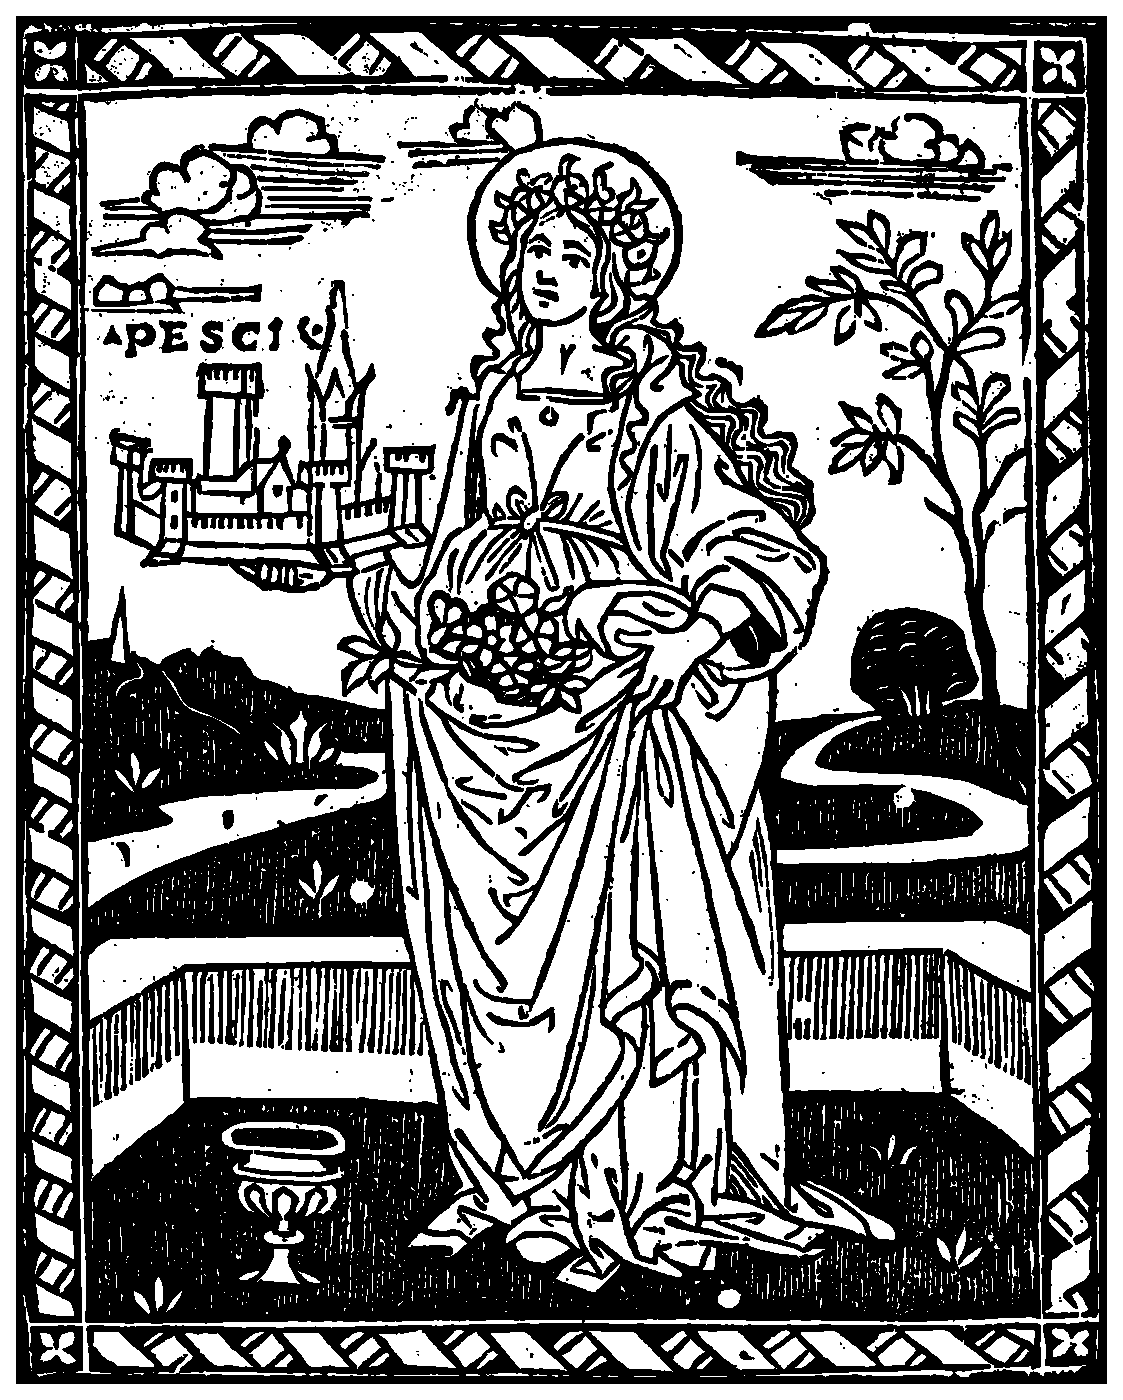
\includegraphics[width=98mm, height=122.916mm]{Propers/Dorothy.eps}
    \caption{\textsc{\Huge{Proper of Saints}}}
\end{figure}
\fancyhead[C]{{\LARGE Proper of Saints}}
\fancyhead[RO,LE]{}
\fancyhead[RE,LO]{}
\phantomsection
\addcontentsline{toc}{section}{Through the Year}

\begin{rubric}
	Propers for Memorials are indicated by parentheses: ().
\end{rubric}

\begin{rubric}
	\textsc{Note,} When a Common is mentioned, it is used for the propers of the Feast Day, except for anything provided for the Feast Day itself.
\end{rubric}

\festival{Vigil}{29 November}{Vigil of St. Andrew}
\feastday{St. Andrew Vigil}
\feastdate{29}{November}

\begin{rubric}
	If \blackrubric{the Festival of St. Andrew} fall on a Monday, then the anticipated Vigil of St. Andrew is kept on the preceding Saturday, but the Commemoration of St. Saturninus is omitted, in which case Commemoration \blackrubric{of St. Mary} (p. \pageref{SPMaryInAdvent}) \& \blackrubric{Against the Persecutors of the Church} (p. \pageref{SPAgainst}) or \blackrubric{for the Chief Bishop} (p. \pageref{SPChiefBishop}).
\end{rubric}

\introit
\lett{T}{he} Lord, walking by the sea of Galilee, saw two brethren, Peter and Andrew, and he called them, saying: Follow me: I will make you fishers of men. \textit{Ps.} The heavens declare the glory of God: and the firmament sheweth his handy-work.

\collect
\lett{W}{e} beseech thee, Almighty God: that the blessed Apostle Andrew, whose festival we prevent, may implore thy help for us; that we, being absolved from our offences, may likewise be delivered from all dangers. Through.

\begin{rubric}
	In Advent, Commemoration \blackrubric{of the Feria} \& \blackrubric{of St. Saturninus} (p. \pageref{SaturninusCollect}).
\end{rubric}
\begin{rubric}
	Outside of Advent, Commemoration \blackrubric{of St. Saturninus} (p. \pageref{SaturninusCollect}) \& \blackrubric{of St. Mary in Eastertide} (p. \pageref{SPMaryInEaster}).
\end{rubric}

\readingcitation{Epistle}{Ecclesiasticus 44:22}
\lett{I}{n} Isaac did the Lord establish, for Abraham his father's sake, The blessing of all men, and the covenant: And he made it rest upon the head of Jacob; He acknowledged him in his blessings, And gave to him by inheritance, And divided his portions; Among twelve tribes did he part them. And he brought out of him a man of mercy, Which found favour in the sight of all flesh; A man beloved of God and men, even Moses, Whose memorial is blessed. He made him like to the glory of the saints, And magnified him in the fears of his enemies. By his words he caused the wonders to cease; He glorified him in the sight of kings; He gave him commandment for his people, And shewed him part of his glory. He sanctified him in his faithfulness and meekness; He chose him out of all flesh. He made him to hear his voice, And led him into the thick darkness, And gave him commandments face to face, Even the law of life and knowledge, That he might teach Jacob the covenant, And Israel his judgments. He exalted Aaron, a holy man like unto him, Even his brother, of the tribe of Levi. He established for him an everlasting covenant, And gave him the priesthood of the people; He beautified him with comely ornaments, And girded him about with a robe of glory.

\gradual{Right honourable are thy friends, O God: right well is their princedom established. ℣. If I tell them: they are more in number than the sand.}

\readingcitation{Gospel}{John 1:35}
\lett{A}{t that time:} John stood, and two of his disciples; And looking upon Jesus as he walked, he saith, Behold the Lamb of God! And the two disciples heard him speak, and they followed Jesus. Then Jesus turned, and saw them following, and saith unto them, What seek ye? They said unto him, Rabbi, (which is to say, being interpreted, Master,) where dwellest thou? He saith unto them, Come and see. They came and saw where he dwelt, and abode with him that day: for it was about the tenth hour. One of the two which heard John speak, and followed him, was Andrew, Simon Peter's brother. He first findeth his own brother Simon, and saith unto him, We have found the Messias, which is, being interpreted, the Christ. And he brought him to Jesus. And when Jesus beheld him, he said, Thou art Simon the son of Jona: thou shalt be called Cephas, which is by interpretation, A stone. The day following Jesus would go forth into Galilee, and findeth Philip, and saith unto him, Follow me. Now Philip was of Bethsaida, the city of Andrew and Peter. Philip findeth Nathanael, and saith unto him, We have found him, of whom Moses in the law, and the prophets, did write, Jesus of Nazareth, the son of Joseph. And Nathanael said unto him, Can there any good thing come out of Nazareth? Philip saith unto him, Come and see. Jesus saw Nathanael coming to him, and saith of him, Behold an Israelite indeed, in whom is no guile! Nathanael saith unto him, Whence knowest thou me? Jesus answered and said unto him, Before that Philip called thee, when thou wast under the fig tree, I saw thee. Nathanael answered and saith unto him, Rabbi, thou art the Son of God; thou art the King of Israel. Jesus answered and said unto him, Because I said unto thee, I saw thee under the fig tree, believest thou? thou shalt see greater things than these. And he saith unto him, Verily, verily, I say unto you, Hereafter ye shall see heaven open, and the angels of God ascending and descending upon the Son of man.

\offertory{Thou hast crowned him with glory and worship: thou hast made him to have dominion of the works of thy hands, O Lord.}

\secret
\lett{W}{e} offer, O Lord, this gift to be hallowed unto thee: whereby, recalling the festival of thy blessed Apostle Andrew, we likewise implore the purification of our souls. Through.

\begin{rubric}
	In Advent, Commemoration \blackrubric{of the Feria} \& \blackrubric{of St. Saturninus} (p. \pageref{SaturninusSecret}).
\end{rubric}
\begin{rubric}
	Outside of Advent, Commemoration \blackrubric{of St. Saturninus} (p. \pageref{SaturninusSecret}) \& \blackrubric{of St. Mary in Eastertide} (p. \pageref{SPMaryInEaster}).
\end{rubric}

\communion{Andrew saith to Simon his brother: We have found the Messias, which is called the Christ: and he brought him to Jesus.}

\postcommunion
\lett{O}{Lord,} who hast bestowed on us these sacraments, we humbly beseech thee: that, at the intercession of thy blessed Apostle Andrew, the mysteries which we offer for his venerable passion may be profitable for our healing. Through.

\begin{rubric}
	In Advent, Commemoration \blackrubric{of the Feria} \& \blackrubric{of St. Saturninus} (p. \pageref{SaturninusPostcommunion}).
\end{rubric}
\begin{rubric}
	Outside of Advent, Commemoration \blackrubric{of St. Saturninus} (p. \pageref{SaturninusPostcommunion}) \& \blackrubric{of St. Mary in Eastertide} (p. \pageref{SPMaryInEaster}).
\end{rubric}


\subbymemorial{29 November}{St. Saturninus}
\feastday{{St. Saturninus}}
\feastdate{29}{November}

\begin{rubric}
	The Second Common of a Martyr not a Bishop (p. \pageref{CommonMartyrNotBishopII}).
\end{rubric}

\collect\label{SaturninusCollect}
\lett{O}{God,} who vouchsafest unto us to rejoice in the birthday of thy blessed Martyr Saturninus: grant, we pray thee; that we may be succoured by his merits. Through.

\secret\label{SaturninusSecret}
\lett{S}{anctify,} O Lord, we beseech thee, the offerings which we dedicate unto thee: and at the intercession of blessed Saturninus, thy Martyr, for their sake graciously regard us. Through.

\postcommunion\label{SaturninusPostcommunion}
\lett{W}{e} beseech thee, O Lord, that we, being sanctified by the receiving of thy sacrament: may, at the intercession of thy Saints, be thereby rendered acceptable unto thee. Through.


\festival{Second Class Double}{30 November}{St. Andrew}
\feastday{St. Andrew}
\feastdate{30}{November}

\introit
\lett{R}{ight} honourable are thy friends unto me, O God: right well is their princedom established. \textit{Ps.} O Lord, thou hast searched me out, and known me: thou knowest my down-sitting, and mine uprising.

\collect
\lett{W}{e} humbly entreat thy Majesty, O Lord: that as blessed Andrew the Apostle was to thy Church a preacher and governor; so he may be a perpetual intercessor for us in thy sight. Through.

\begin{rubric}
    In Advent, Commemoration \blackrubric{of the Feria.}
\end{rubric}

\readingcitation{Epistle}{Romans 10:9}
\lett{B}{rethren:} If thou shalt confess with thy mouth the Lord Jesus, and shalt believe in thine heart that God hath raised him from the dead, thou shalt be saved. For with the heart man believeth unto righteousness; and with the mouth confession is made unto salvation. For the scripture saith, Whosoever believeth on him shall not be ashamed. For there is no difference between the Jew and the Greek: for the same Lord over all is rich unto all that call upon him. For whosoever shall call upon the name of the Lord shall be saved. How then shall they call on him in whom they have not believed? and how shall they believe in him of whom they have not heard? and how shall they hear without a preacher? And how shall they preach, except they be sent? as it is written, How beautiful are the feet of them that preach the gospel of peace, and bring glad tidings of good things! But they have not all obeyed the gospel. For Esaias saith, Lord, who hath believed our report? So then faith cometh by hearing, and hearing by the word of God. But I say, Have they not heard? Yes verily, their sound went into all the earth, and their words unto the ends of the world. But I say, Did not Israel know? First Moses saith, I will provoke you to jealousy by them that are no people, and by a foolish nation I will anger you. But Esaias is very bold, and saith, I was found of them that sought me not; I was made manifest unto them that asked not after me. But to Israel he saith, All day long I have stretched forth my hands unto a disobedient and gainsaying people.

\gradall{Thou shalt make them princes in all lands: they shall remember thy name, O Lord. ℣. Instead of thy fathers thou shalt have children: therefore shall the people give thanks unto thee.}{Alleluia, alleluia. ℣. The Lord loved Andrew as a sweet savour. Alleluia.}

\readingcitation{Gospel}{Matthew 4:18}
\lett{A}{t that time:} Jesus, walking by the sea of Galilee, saw two brethren, Simon called Peter, and Andrew his brother, casting a net into the sea: for they were fishers. And he saith unto them, Follow me, and I will make you fishers of men. And they straightway left their nets, and followed him. And going on from thence, he saw other two brethren, James the son of Zebedee, and John his brother, in a ship with Zebedee their father, mending their nets; and he called them. And they immediately left the ship and their father, and followed him.
\offertory{Right honourable are thy friends unto me, O God: right well is their princedom established.}
\secret
\lett{O}{Lord,} we beseech thee that the holy prayer of thy blessed Apostle Andrew may commend our sacrifice unto thee: that it may be rendered acceptable by the merits of him in whose honour it is solemnly shewn forth. Through.
\begin{rubric}
    In Advent, Commemoration \blackrubric{of the Feria.}
\end{rubric}

\communion{Follow me: I will make you fishers of men: and they straightway left their nets, and followed the Lord.}
\postcommunion
\lett{W}{e} beseech thee, O Lord, that these divine mysteries, which we have joyfully received on the festivity (commemoration) of blessed Andrew thine Apostle: may effectually avail for the glory of thy Saints, and likewise for our pardon. Through.
\begin{rubric}
    In Advent, Commemoration \blackrubric{of the Feria.}
\end{rubric}


%MANUAL ADJUSTMENT:
\clearpage
\festival{Double}{2 December}{St. Peter Chrysologus}
\feastday{{St. Peter Chrysologus}}
\feastdate{2}{December}

\begin{rubric}
	The Common of Doctors (p. \pageref{CommonDoctors}), with Commemoration \blackrubric{of St. Bibiana,} as below, and \blackrubric{of the Advent Feria.}
\end{rubric}

%MANUAL ADJUSTMENT:
\vspace{-0.5\baselineskip}

\collect

%MANUAL ADJUSTMENT:
\vspace{-0.2\baselineskip}

\lett{O}{God,} who by divine foreshewing wast pleased to choose blessed Peter Chrysologus thy illustrious Doctor to rule and instruct thy Church: grant, we beseech thee; that, as we have had him for a Doctor of life on earth, so we may be found worthy to have him for an intercessor in heaven. Through.

\gradual{Behold a great priest, who in his days pleased God. ℣. There was none found like unto him, who kept the law of the Most High.}

\communion{Lord. thou deliveredst unto me five talents: behold, I have gained beside them five talents more. Well done, thou good and faithful servant, thou hast been faithful over a few things, I will make thee ruler over many things, enter thou into the joy of thy lord.}

\subbymemorial{2 December}{St. Bibiana}
\feastday{{St. Bibiana}}
\feastdate{2}{December}

\begin{rubric}
	The Second Common of a Virgin Martyress (p. \pageref{CommonVirginMartyrII}).
\end{rubric}

%MANUAL ADJUSTMENT:
\vspace{-0.35\baselineskip}

\collect

%MANUAL ADJUSTMENT:
\vspace{-0.2\baselineskip}

\lett{O}{God,} the giver of all good gifts, who in thy handmaid Bibiana didst unite the palm of martyrdom with the flower of virginity: unite by her intercession our hearts in charity with thee; that all perils being done away, we may attain unto everlasting rewards. Through.

%MANUAL ADJUSTMENT:
\vspace{-0.3\baselineskip}

\secret

%MANUAL ADJUSTMENT:
\vspace{-0.15\baselineskip}

\lett{G}{raciously} receive, O Lord, through the merits of blessed Bibiana, thy Virgin and Martyress, the sacrifices which we offer unto thee: and grant that they may avail for our continual help. Through.

%MANUAL ADJUSTMENT:
\vspace{-0.3\baselineskip}

\postcommunion

%MANUAL ADJUSTMENT:
\vspace{-0.15\baselineskip}

\lett{O}{Lord} our God, who hast fulfilled us with the bounty of thy heavenly gift: we beseech thee, at the intercession of blessed Bibiana, thy Virgin and Martyress, we may ever live by the partaking of the same. Through.


%MANUAL ADJUSTMENT:
\clearpage
\subbymemorial{4 December}{St. Barbara}
\feastday{{St. Barbara}}
\feastdate{4}{December}

\begin{rubric}
	The First Common of a Virgin Martyress (p. \pageref{CommonVirginMartyrI}).
\end{rubric}


\subbymemorial{5 December}{St. Sabbas of Jud{\ae}a}
\feastday{{St. Sabbas}}
\feastdate{5}{December}

\begin{rubric}
	The Common of Abbots (p. \pageref{CommonAbbots}).
\end{rubric}

\begin{rubric}
	If today be Saturday, the Mass is \blackrubric{of St. Mary on Saturday} (p. \pageref{MarySaturday}) with Commemoration \blackrubric{of the Feria} \& \blackrubric{of St. Sabbas.}
\end{rubric}


\festival{Double}{6 December}{St. Nicholas}
\feastday{{St. Nicholas}}
\feastdate{6}{December}

\introit
\lett{T}{he} Lord hath established a covenant of peace with him, and made him a prince: that he should have the dignity of the priesthood for ever. \textit{Ps.} Lord, remember David: and all his trouble.

\collect
\lett{O}{God,} who didst adorn thy blessed Bishop Nicholas with innumerable miracles: grant, we beseech thee; that by his merits and prayers we may be delivered from the fires of hell. Through.

\begin{rubric}
	Commemoration \blackrubric{of the Feria.}
\end{rubric}

\readingcitation{Epistle}{Hebrews 13:7}
\lett{B}{rethren:} Remember them which have the rule over you, who have spoken unto you the word of God: whose faith follow, considering the end of their conversation. Jesus Christ the same yesterday, and to day, and for ever. Be not carried about with divers and strange doctrines. For it is a good thing that the heart be established with grace; not with meats, which have not profited them that have been occupied therein. We have an altar, whereof they have no right to eat which serve the tabernacle. For the bodies of those beasts, whose blood is brought into the sanctuary by the high priest for sin, are burned without the camp. Wherefore Jesus also, that he might sanctify the people with his own blood, suffered without the gate. Let us go forth therefore unto him without the camp, bearing his reproach. For here have we no continuing city, but we seek one to come. By him therefore let us offer the sacrifice of praise to God continually, that is, the fruit of our lips giving thanks to his name. But to do good and to communicate forget not: for with such sacrifices God is well pleased. Obey them that have the rule over you, and submit yourselves: for they watch for your souls, as they that must give account.

\gradall{I have found David my servant, with my holy oil have I anointed him: my hand shall hold him fast, and my arm shall strengthen him. ℣. The enemy shall not be able to do him violence, the son of wickedness shall not hurt him.}{Alleluia, alleluia. ℣. The righteous shall flourish like a palm-tree: and shall spread abroad like a cedar in Libanus. Alleluia.}

%MANUAL ADJUSTMENT:
\vspace{-0.4\baselineskip}

\readingcitation{Gospel}{Matthew 25:14}

%MANUAL ADJUSTMENT:
\vspace{-0.1\baselineskip}

\lett{A}{t that time:} Jesus spake this parable to his disciples: A man travelling into a far country, who called his own servants, and delivered unto them his goods. And unto one he gave five talents, to another two, and to another one; to every man according to his several ability; and straightway took his journey. Then he that had received the five talents went and traded with the same, and made them other five talents. And likewise he that had received two, he also gained other two. But he that had received one went and digged in the earth, and hid his lord's money. After a long time the lord of those servants cometh, and reckoneth with them. And so he that had received five talents came and brought other five talents, saying, Lord, thou deliveredst unto me five talents: behold, I have gained beside them five talents more. His lord said unto him, Well done, thou good and faithful servant: thou hast been faithful over a few things, I will make thee ruler over many things: enter thou into the joy of thy lord. He also that had received two talents came and said, Lord, thou deliveredst unto me two talents: behold, I have gained two other talents beside them. His lord said unto him, Well done, good and faithful servant; thou hast been faithful over a few things, I will make thee ruler over many things: enter thou into the joy of thy lord.

\offertory{My truth and my mercy shall be with him: and in my name shall his horn be exalted.}

%MANUAL ADJUSTMENT:
\vspace{-0.4\baselineskip}

\secret

%MANUAL ADJUSTMENT:
\vspace{-0.1\baselineskip}

\lett{S}{anctify,} we beseech thee, O Lord God, these gifts which we offer on the solemnity of thy holy Bishop Nicholas: that our life may ever thereby be directed both in prosperity and in adversity. Through.

\begin{rubric}
	Commemoration \blackrubric{of the Feria.}
\end{rubric}

\communion{I have sworn once by my holiness: His seed shall endure for ever, and his seat is like as the sun before me, he shall stand fast for evermore as the moon, and as the faithful witness in heaven.}

\postcommunion
\lett{M}{ay} the sacrifices which we have received, O Lord, for the solemnity of thy holy Bishop Nicholas, preserve us by their everlasting protection. Through.

\begin{rubric}
	Commemoration \blackrubric{of the Feria.}
\end{rubric}


\festival{Greater Double}{7 December}{St. Ambrose}
\feastday{{St. Ambrose}}
\feastdate{7}{December}

\introit
\lett{I}{n} the midst of the Church he opened his mouth: and the Lord filled him with the spirit of wisdom and of understanding: he clothed him with a robe of glory. \textit{Ps.} It is a good thing to give thanks unto the Lord: and to sing praises unto thy name, O most Highest.

\collect
\lett{O}{God,} who didst give blessed Ambrose unto thy people to be a minister of everlasting salvation: grant, we beseech thee; that as we have learned of him the doctrine of life on earth, so we may be found worthy to have him for our advocate in heaven. Through.

\begin{rubric}
	Commemoration \blackrubric{of the Feria.}
\end{rubric}

\begin{rubric}
	The Epistle is from the Common of Doctors (p. \pageref{CommonDoctorsEpistle}).
\end{rubric}

\gradall{Behold a great priest, who in his days pleased God. ℣. There was none foun like unto him, who kept the law of the Most High.}{Alleluia, alleluia. ℣. The Lord sware, and will not repent: Thou art a priest for ever after the order of Melchisedech.}

\tractnotice
\tract{Blessed is the man that feareth the Lord: he hath great delight in his commandments. ℣. His seed shall be mighty upon earth: the generation of the faithful shall be blessed. ℣. Riches and plenteousness shall be in his house: and his righteousness endureth for ever.}

\alleluianotice
\alleluia{Alleluia, alleluia. ℣. The Lord loved him, and adorned him: and clothed him with a robe of glory. Alleluia. ℣. The righteous shall grow as the lily and flourish for ever before the Lord. Alleluia.}

\begin{rubric}
	The Gospel is from the Common of Doctors (p. \pageref{CommonDoctorsGospel}).
\end{rubric}

\offertory{My truth and my mercy shall be with him: and in my name shall his horn be exalted.}

\secret
\lett{A}{lmighty} and everlasting God, grant, that the gifts which we present unto thy Majesty, may through the intercession of blessed Ambrose, thy Confessor and Bishop, be profitable unto us for everlasting salvation. Through.

\begin{rubric}
	Commemoration \blackrubric{of the Feria.}
\end{rubric}

\communion{I have sworn once by my holiness: His seed shall endure for ever, and his seat is like as the sun before me, he shall stand fast for evermore as the moon, and as the faithful witness in heaven.}

\postcommunion
\lett{G}{rant,} we beseech thee, Almighty God: that we, receiving the sacraments of our salvation, may ever be aided by the prayer of blessed Ambrose thy Confessor and Bishop; in whose honour we have made these offerings unto thy Majesty. Through.

\begin{rubric}
	Commemoration \blackrubric{of the Feria.}% In Lent, the Last Gospel \blackrubric{of the Feria.}
\end{rubric}


\festival{Second Class Double, Common Octave}{8 December}{Conception of the Blessed Virgin Mary}\label{ConceptionBVM}
\feastday{Conception B.V.M.}
\feastdate{8}{December}

\introit
\lett{L}{et} us all rejoice in the Lord, and celebrate this feast in honour of the Virgin Mary, at whose Conception Angels rejoice and praise the Son of God. \textit{Ps.} My heart is inditing of a good matter: I speak of the things which I have made unto the King.

\collect
\lett{O}{God,} mercifully hear the supplication of thy servants; that we who are assembled together on the Conception of the Virgin Mother of God, may at her intercession be delivered by thee from the dangers which beset us. Through.
\begin{rubric}
    Commemoration \blackrubric{of the Feria.}
\end{rubric}

\readingcitation{Epistle}{Ecclesiasticus 24:17}
\lett{A}{s} the vine I put forth grace; And my flowers are the fruit of glory and riches. Come unto me, ye that are desirous of me, And be ye filled with my produce. For my memorial is sweeter than honey, And mine inheritance than the honeycomb. They that eat me shall yet be hungry; And they that drink me shall yet be thirsty. He that obeyeth me shall not be ashamed; And they that work in me shall not do amiss.

\gradall{Hearken, O daughter, and consider: incline thine ear. So shall the king have pleasure in thy beauty. ℣. According to thy worship and renown, good luck have thou with thine honour: ride on, because of the word of truth, of meekness, and righteousness; and thy right hand shall teach thee terrible things.}{Alleluia, alleluia. ℣. The Conception of the glorious Virgin Mary who sprang from the seed of Abraham, of the tribe of Judah, of the root of David. Alleluia.}

\subsubsection{Sequence}
\begin{multicols}{2}
\begin{hangparas}{1.25em}{1}
On this great day, we celebrate

And piously we estimate

Mary's holy conception.\\

2. Begotten is the Mother Maid,

Conceiv'd, created, channel made

Of pardon to sinful man.\\

3. Adam's primeval banishment

%MANUAL CHANGE BASED ON LATIN:
Joachim's childless discontent

There find their salvation.\\

4. This the Prophets have foreshown,

This was to the Patriarchs known:

Son, to Mother, gives her birth.\\

5. The Virgin whence a flower springs,

The Star which forth the Sun should bring,

On this day is conceived;\\

6. The flow'r which from the rod should bloom,

The Sun which of the Star should come,

Is her Christ interpreted.%MANUAL ADJUSTMENT:\\

7. O how happy, O how radiant!

Dear to God, to us how brilliant,

Hath this her Conception been!\\

8. Misery now is at an end,

His mercy doth on earth descend,

For sorrow is given joy.\\

9. A Mother new new offspring bears,

From a new Star new Sun appears,

New grace doth all inspire;\\

10. Mother bears the Generator,

Creature brings forth the Creator,

The Daughter bears the Sire:\\

11. O unexampled novelty!

O new, unheard of dignity!

Mother's holy chastity!\\

12. The Son's Conception without guile!

Rejoice, O gracious Virgin mild!

Fair rod with blossoms undefil'd,

Mother ennobled by her Child,

Such grace can no other know.\\

13. That which lay hid, in figure seal'd,

By clouds mysterious conceal'd,

The future Mother hath reveal'd:

For once a Virgin pure and good

Reversed the laws of Motherhood:

Nature, surpris'd, beheld a flood

Of Deity outpoured.\\

\selectlanguage{latin}

14. Triste fuit in Eva ve,

Sed ex Eva formans Ave,

Versa vice, sed non prave

Intus ferens in conclave

Verbum bonum et suave

Nobis, Mater Virgo, fave

Tua frui gratia.\\

\selectlanguage{british}

15. Whoe'er thou art, without delay

Open thy lips, her praises pay;

Offer her homage, to her pray

At every hour, on every day.

With swelling voice, with spirit sage,

By supplicating prayer engage

A part in her patronage.\\

16. Thou of the sad art comfort sure,

True Mother of the orphans poor,

Of the opprest the help secure,

Thou of the sick the healing cure,

All things to all thou givest.\\

17. With one consent we ask of thee,

Whom praise awaits especially,

Conduct us wanderers o'er this sea

Unto salvation's port, where we

By grace may be at true rest. Amen.
\end{hangparas}
\end{multicols}

\readingcitation{Gospel}{Matthew 1:1}
\lett{T}{he} book of the generation of Jesus Christ, the son of David, the son of Abraham. Abraham begat Isaac; and Isaac begat Jacob; and Jacob begat Judas and his brethren; And Judas begat Phares and Zara of Thamar; and Phares begat Esrom; and Esrom begat Aram; And Aram begat Aminadab; and Aminadab begat Naasson; and Naasson begat Salmon; And Salmon begat Booz of Rachab; and Booz begat Obed of Ruth; and Obed begat Jesse; And Jesse begat David the king; and David the king begat Solomon of her that had been the wife of Urias; And Solomon begat Roboam; and Roboam begat Abia; and Abia begat Asa; And Asa begat Josaphat; and Josaphat begat Joram; and Joram begat Ozias; And Ozias begat Joatham; and Joatham begat Achaz; and Achaz begat Ezekias; And Ezekias begat Manasses; and Manasses begat Amon; and Amon begat Josias; And Josias begat Jechonias and his brethren, about the time they were carried away to Babylon: And after they were brought to Babylon, Jechonias begat Salathiel; and Salathiel begat Zorobabel; And Zorobabel begat Abiud; and Abiud begat Eliakim; and Eliakim begat Azor; And Azor begat Sadoc; and Sadoc begat Achim; and Achim begat Eliud; And Eliud begat Eleazar; and Eleazar begat Matthan; and Matthan begat Jacob; And Jacob begat Joseph the husband of Mary, of whom was born Jesus, who is called Christ.

\offertory{Full of grace are thy lips, because God hath blessed thee for ever.}

\secret
\lett{O}{Lord,} let the human nature of thine only-begotten succour us, that he, who being born of a Virgin diminished not but sanctified the chastity of his Mother, may put away our offences from us on the feast of her Conception, and make our oblations acceptable to himself, even Jesus Christ our Lord. Who liveth.
\begin{rubric}
    Commemoration \blackrubric{of the Feria.}
\end{rubric}

\communion{Thy Son's true faith hath cleansed the world of sin. Immaculate thy virginity abideth.}

\postcommunion
\lett{G}{rant,} we beseech thee, O Lord, that the sacrament which we have received of our bounden duty on this yearly celebration, may, at the intercession of blessed Mary ever-Virgin, afford us relief in this present life and in the world to come. Through.
\begin{rubric}
    Commemoration \blackrubric{of the Feria.}
\end{rubric}


\subbymemorial{10 December}{St. Melchiades}
\feastday{{St. Melchiades}}
\feastdate{10}{December}

\begin{rubric}
	The First Common of a Martyr Bishop (p. \pageref{CommonMartyrBishopI}).
\end{rubric}


%MANUAL ADJUSTMENT:
\clearpage
\subbymemorial{11 December}{St. Damasus}
\feastday{{St. Damasus}}
\feastdate{11}{December}

\introit
\lett{L}{et} thy priests, O Lord, be clothed with righteousness, and let thy Saints sing with joyfulness: for thy servant David's sake turn not away the presence of thine Anointed. \textit{Ps.} Lord, remember David: and all his trouble.

\collect
\lett{G}{raciously} hear our prayers, O Lord: and at the intercession of blessed Damasus, thy Confessor and Bishop, mercifully grant us pardon and peace. Through.

\begin{rubric}
	Commemoration \blackrubric{of the Octave} \& \blackrubric{of the Feria.}
\end{rubric}

\begin{rubric}
	The Epistle is from the Second Common of a Confessor Bishop (p. \pageref{CommonConfessorBishopIIEpistle}).
\end{rubric}

\gradall{Behold a great priest who in his days pleased God. ℣. There was none found like unto him, who kept the law of the Most High.}{Alleluia, alleluia. ℣. Thou art a priest for ever after the order of Melchisedech. Alleluia.}

\begin{rubric}
	The Gospel is from the Second Common of a Confessor Bishop (p. \pageref{CommonConfessorBishopIIGospel}).
\end{rubric}

\communion{I have found David my servant, with my holy oil have I anointed him: my hand shall hold him fast, and my arm shall strengthen him.}

\secret
\lett{G}{rant,} O Lord, that like as thy dedicated people do acknowledge that in tribulation they have been succoured by the merits of thy Saints: so this oblation, which they offer unto thee in honour of the same, may be acceptable in thy sight. Through.

\begin{rubric}
	Commemoration \blackrubric{of the Octave} \& \blackrubric{of the Feria.}
\end{rubric}

\communion{Lord, thou deliveredst unto me five talents, behold I have gained beside them five talents more. Well done, thou good and faithful servant, thou hast been faithful over a few things, I will make thee ruler over many things, enter thou into the joy of thy Lord.}

\postcommunion
\lett{G}{rant,} we beseech thee, O Lord, that thy faithful people may ever rejoice in the veneration of thy saints: and be defended by their perpetual supplication. Through.

\begin{rubric}
	Commemoration \blackrubric{of the Octave} \& \blackrubric{of the Feria.}
\end{rubric}


\festival{Greater Double}{13 December}{St. Lucy}
\feastday{{St. Lucy}}
\feastdate{13}{December}

\introit
\lett{T}{hou} hast loved righteousness, and hated iniquity: wherefore God, even thy God, hath anointed thee with the oil of gladness above thy fellows. \textit{Ps.} My heart is inditing of a good matter: I speak of the things which I have made unto the King.

\collect
\lett{G}{raciously} hear us, O God of our salvation: that, like as we do rejoice in the festival of blessed Lucy thy Virgin; so we may be instructed in all godly and devout affection. Through.

\begin{rubric}
	Commemoration \blackrubric{of the Octave} \& \blackrubric{of the Feria.}
\end{rubric}

\begin{rubric}
	The Epistle is from the First Common of a Virgin (p. \pageref{CommonVirginOnlyIEpistle}).
\end{rubric}

\gradall{Thou hast loved righteousness, and hated iniquity. ℣. Wherefore God, even thy God, hath anointed thee with the oil of gladness.}{Alleluia, alleluia. ℣. Full of grace are thy lips: because God hath blessed thee for ever. Alleluia.}

\begin{rubric}
	In Votive Masses after Septuagesima, the Tract, and in Eastertide, the Alleluia, is from the First Common of a Virgin (p. \pageref{CommonVirginOnlyI}).
\end{rubric}

\readingcitation{Gospel}{Matthew 13:44}
\lett{A}{t that time:} Jesus spake this parable unto his disciples: The kingdom of heaven is like unto treasure hid in a field; the which when a man hath found, he hideth, and for joy thereof goeth and selleth all that he hath, and buyeth that field. Again, the kingdom of heaven is like unto a merchant man, seeking goodly pearls: Who, when he had found one pearl of great price, went and sold all that he had, and bought it. Again, the kingdom of heaven is like unto a net, that was cast into the sea, and gathered of every kind: Which, when it was full, they drew to shore, and sat down, and gathered the good into vessels, but cast the bad away. So shall it be at the end of the world: the angels shall come forth, and sever the wicked from among the just, And shall cast them into the furnace of fire: there shall be wailing and gnashing of teeth. Jesus saith unto them, Have ye understood all these things? They say unto him, Yea, Lord. Then said he unto them, Therefore every scribe which is instructed unto the kingdom of heaven is like unto a man that is an householder, which bringeth forth out of his treasure things new and old.

\offertory{The Virgins that be her fellows shall be brought unto the King: they that bear her company shall be brought unto thee with joy and gladness: and shall enter into the palace of the Lord the King.}

\secret
\lett{G}{rant,} O Lord, that like as thy dedicated people do acknowledge that in tribulation they have been succoured by the merits of thy Saints: so this oblation, which they offer unto thee in honour of the same, may be acceptable in thy sight. Through.

\begin{rubric}
	Commemoration \blackrubric{of the Octave} \& \blackrubric{of the Feria.}
\end{rubric}

\communion{Princes have persecuted me without a cause, but my heart standeth in awe of thy word: I am as glad of thy word, as one that findeth great spoils.}

\postcommunion
\lett{O}{Lord,} who hast satisfied thy family with sacred gifts: we beseech thee; that we may at all times be comforted by the intercession of her whose festival we celebrate. Through.

\begin{rubric}
	Commemoration \blackrubric{of the Octave} \& \blackrubric{of the Feria.}
\end{rubric}


\subbymemorial{13 December}{St. Herman of Alaska}
\feastday{{St. Herman Alaska}}
\feastdate{13}{December}

\begin{rubric}
	The First Common of a Confessor not Bishop (p. \pageref{CommonConfessorNotBishopI}).
\end{rubric}


%MANUAL ADJUSTMENT:
\clearpage
\festival{Semidouble}{14 December}{Day VII within the Octave of the Conception}
\feastday{{Conception Octave}}
\feastdate{14}{December}

\begin{rubric}
	Of the Octave, as on December 9. But if Ember Wednesday fall on this day, of the Ember Day, with a Commemoration \blackrubric{of the Octave} \& \blackrubric{of the Holy Ghost} (p. \pageref{SPHolyGhost}).
\end{rubric}

\begin{rubric}
	\textsc{Note,} If an Ember Day occur on any of the following Feasts, the Commemoration \blackrubric{of the Feria} is omitted.
\end{rubric}


\festival{Greater Double}{15 December}{Octave Day of the Conception of the Blessed Virgin Mary}
\feastday{{Conception Octave Day}}
\feastdate{15}{December}

\begin{rubric}
	Mass as on the Feast (p. \pageref{ConceptionBVM}), with Commemoration \blackrubric{of the Feria.}
\end{rubric}


\subbymemorial{16 December}{St. Eusebius of Vercelli}
\feastday{{St. Eusebius}}
\feastdate{16}{December}

\begin{rubric}
	The Second Common of a Martyr Bishop (p. \pageref{CommonMartyrBishopII}), with Commemoration \blackrubric{of the Feria} \& \blackrubric{of St. Mary in Advent} (p. \pageref{SPMaryInAdvent}).
\end{rubric}


\festival{Greater Double}{18 December}{Expectation of the Blessed Virgin Mary}
\feastday{{Expectation B.V.M.}}
\feastdate{18}{December}

\begin{rubric}
	The Common of the Blessed Virgin Mary (p. \pageref{CommonBVM}).
\end{rubric}

\collect
\lett{O}{God,} who wast pleased that thy Word should take flesh of the womb of the Blessed Virgin Mary at the message of an Angel: grant to thy humble servants; that we who believe her to be truly the Mother of God may be aided by her intercession in thy sight. Through the same.


\festival{Vigil}{20 December}{Vigil of St. Thomas}
\feastday{{St. Thomas Vigil}}
\feastdate{20}{December}

\begin{rubric}
	The Common of the Vigil of Apostles (p. \pageref{CommonVigilApostles}).
\end{rubric}
\begin{rubric}
	Commemoration of \blackrubric{of the Feria} \& \blackrubric{of the Saints} (p. \pageref{SPSaints}). But if an Ember Day occur, Commemoration \blackrubric{of the Vigil} in the Mass \blackrubric{of the Feria.}
\end{rubric}

\begin{rubric}
	If \blackrubric{the Festival of St. Thomas} fall on a Monday, then in the Ember Saturday Mass, Commemoration \blackrubric{of the anticipated Vigil of St. Thomas} (the Last Gospel of the Vigil being read at the end) \& \blackrubric{of St. Mary in Advent} (p. \pageref{SPMaryInAdvent}).
\end{rubric}


%MANUAL ADJUSTMENT:
\clearpage
\festival{Second Class Double}{21 December}{St. Thomas}
\feastday{St. Thomas}
\feastdate{21}{December}

\introit
\lett{R}{ight} honourable are thy friends unto me, O God: right well is their princedom established. \textit{Ps.} O Lord, thou hast searched me out, and known me: thou knowest my down-sitting, and mine uprising.

\collect
\lett{G}{rant} us, we beseech thee, O Lord, to glory in the solemnity of thy blessed Apostle Thomas: that we may ever be succoured by his protection; and follow his faith with worthy devotion. Through.

\begin{rubric}
    Commemoration \blackrubric{of the Feria.}
\end{rubric}

\readingcitation{Epistle}{Ephesians 2:19}
\lett{B}{rethren:} Ye are no more strangers and foreigners, but fellowcitizens with the saints, and of the household of God; and are built upon the foundation of the apostles and prophets, Jesus Christ himself being the chief corner stone; in whom all the building fitly framed together groweth unto an holy temple in the Lord: in whom ye also are builded together for an habitation of God through the Spirit.

\gradall{Right honourable are thy friends, O God: right well is their princedom established. ℣. If I tell them, they are more in number than the sand.}{Alleluia, alleluia. ℣. Rejoice in the Lord, O ye righteous: for it becometh well the just to be thankful. Alleluia.}

\readingcitation{Gospel}{John 20:24}
\lett{A}{t that time:} Thomas, one of the twelve, called Didymus, was not with them when Jesus came. The other disciples therefore said unto him, We have seen the Lord. But he said unto them, Except I shall see in his hands the print of the nails, and put my finger into the print of the nails, and thrust my hand into his side, I will not believe. And after eight days again his disciples were within, and Thomas with them: then came Jesus, the doors being shut, and stood in the midst, and said, Peace be unto you. Then saith he to Thomas, Reach hither thy finger, and behold my hands; and reach hither thy hand, and thrust it into my side: and be not faithless, but believing. And Thomas answered and said unto him, My Lord and my God. Jesus saith unto him, Thomas, because thou hast seen me, thou hast believed: blessed are they that have not seen, and yet have believed. And many other signs truly did Jesus in the presence of his disciples, which are not written in this book: But these are written, that ye might believe that Jesus is the Christ, the Son of God; and that believing ye might have life through his name.

\offertory{Their sound is gone out into all lands: and their words into the ends of the world.}

%MANUAL ADJUSTMENT:
\vspace{-0.5\baselineskip}

\secret

%MANUAL ADJUSTMENT:
\vspace{-0.25\baselineskip}

\lett{W}{e} render unto thee, O Lord, this duty of our bounden service, humbly beseeching thee: that like as we do offer unto thee this sacrifice of praise in honour of the confession of blessed Thomas the Apostle, so by his prayers thou wouldest preserve thy gifts within us. Through.
\begin{rubric}
    Commemoration \blackrubric{of the Feria.}%, except in Conventual Masses if an Ember Day occur.
\end{rubric}

\communion{Reach hither thy hand, and behold the print of the nails: and be not faithless, but believing.}

%MANUAL ADJUSTMENT:
\vspace{-0.5\baselineskip}

\postcommunion

%MANUAL ADJUSTMENT:
\vspace{-0.25\baselineskip}

\lett{A}{ssist} us, O merciful God: and, at the intercession of blessed Thomas the Apostle on our behalf, continue towards us the gifts of thy loving-kindness. Through.
\begin{rubric}
    Commemoration \blackrubric{of the Feria.}%, except in Conventual Masses if an Ember Day occur.
\end{rubric}

\begin{rubric}
   \textsc{Note,} The Last Gospel is read of the Ember Day, if one occur.%, in non-conventual Masses.
\end{rubric}


\subbymemorial{10 January}{St. Paul the First Hermit}
\feastday{{St. Paul Hermit}}
\feastdate{10}{January}

\introit
\lett{T}{he} just shall flourish like a palm-tree: and shall spread abroad like a cedar in Libanus: planted in the house of the Lord: in the courts of the house of our God. \textit{Ps.} It is a good thing to give thanks unto the Lord: and to sing praises unto thy name, O Most Highest.

\collect
\lett{O}{God,} who makest us glad with the yearly solemnity of blessed Paul, thy Confessor: mercifully grant; that, as we now celebrate his birthday, so we may follow the example of his life. Through.

\begin{rubric}
	The Epistle is from the Common of Abbots (p. \pageref{CommonAbbotsEpistle}).
\end{rubric}

\gradall{The just shall flourish like a palm-tree: and shall spread abroad like a cedar in Libanus in the house of the Lord. ℣. To tell of thy loving-kindness early in the morning, and of thy truth in the night-season.}{Alleluia, alleluia. ℣. The just shall grow as the lily: and flourish for ever before the Lord. Alleluia.}

\readingcitation{Gospel}{Matthew 11:25}
\lett{A}{t that time:} Jesus answered and said: I thank thee, O Father, Lord of heaven and earth, because thou hast hid these things from the wise and prudent, and hast revealed them unto babes. Even so, Father: for so it seemed good in thy sight. All things are delivered unto me of my Father: and no man knoweth the Son, but the Father; neither knoweth any man the Father, save the Son, and he to whomsoever the Son will reveal him. Come unto me, all ye that labour and are heavy laden, and I will give you rest. Take my yoke upon you, and learn of me; for I am meek and lowly in heart: and ye shall find rest unto your souls. For my yoke is easy, and my burden is light.

\offertory{The just shall rejoice in thy strength, O Lord: exceeding glad shall he be of thy salvation: thou hast given him his heart's desire.}

\secret
\lett{G}{rant,} we beseech thee, O Lord, that we who, trusting in this our sacrifice of praise, do offer it before thee to the honour of thy Saints: may by the same be delivered from all evils both in this life and that which is to come. Through.

\communion{The just shall rejoice in the Lord, and put his trust in him: and all they that are true of heart shall be glad.}

\postcommunion
\lett{O}{Lord,} our God, who hast refreshed us with heavenly meat and drink, we humbly beseech thee: that we may be defended by the prayers of him in whose memory we have received the same. Through.


\subbymemorial{11 January}{St. Hyginus of Rome}
\feastday{{St. Hyginus Rome}}
\feastdate{11}{January}

\begin{rubric}
	The First Common of a Martyr not a Bishop (p. \pageref{CommonMartyrNotBishopI}).
\end{rubric}


%MANUAL ADJUSTMENT:
\clearpage
\subbymemorial{12 January}{St. Benedict Biscop}
\feastday{{St. Benedict Biscop}}
\feastdate{12}{January}

\begin{rubric}
	The Common of Abbots (p. \pageref{CommonAbbots}).
\end{rubric}

\collect
\lett{O}{God,} by whose gift the blessed Abbot Benedict left all things that he might be made perfect: grant unto all those who have entered upon the path of evangelical perfection, that they may neither look back nor linger in the way; but hastening to thee without stumbling, may lay hold upon eternal life. Through.

\secret
\lett{W}{e} beseech thee, O Lord, that thy holy Abbot Benedict, may may intercede for us: that this sacrifice which we offer and present upon thy holy altar may be profitable unto us for our salvation. Through.

\postcommunion
\lett{L}{et} thy sacrament, O Lord, which we have now received and the prayers of the blessed Abbot Benedict, effectually defend us: that we may both imitate the example of his conversion, and receive the succour of his intercession. Through.


\festival{Double}{14 January}{St. Hilary}
\feastday{{St. Hilary}}
\feastdate{14}{January}

\begin{rubric}
	The Common of Doctors (p. \pageref{CommonDoctors}).
\end{rubric}

\begin{rubric}
	\textsc{Note,} Commemoration is made \blackrubric{of St. Felix,} as below.
\end{rubric}


\subbymemorial{14 January}{St. Felix}
\feastday{{St. Felix}}
\feastdate{14}{January}

\begin{rubric}
	The Second Common of a Martyr not a Bishop (p. \pageref{CommonMartyrNotBishopII}).\par
\end{rubric}

\collect
\lett{G}{rant,} we beseech thee, Almighty God, that the examples of thy Saints may provoke us to a better life: that as we celebrate their festival so we may imitate their actions. Through.

\secret
\lett{W}{e} beseech thee, O Lord, mercifully to accept this our sacrifice, which we offer unto thee, pleading the merits of blessed Felix, thy Martyr: that the same may avail for our perpetual succour. Through.

\postcommunion
\lett{O}{Lord,} who hast fulfilled us with saving mysteries: we beseech thee that we may be aided by the prayers of blessed Felix thy Martyr, whose festival we celebrate. Through.


\festival{Greater Double}{15 January}{St. Maurus}
\feastday{{St. Maurus}}
\feastdate{15}{January}

\introit
\lett{T}{hy} way is in the sea, and thy paths in the great waters: and thy footsteps are not known. Thou leddest thy people like sheep. \textit{Ps.} The waters saw thee, O God, the waters saw thee, and were afraid: the depths also were troubled.

\collect
\lett{O}{God,} who for a pattern of obedience didst cause blessed Maurus to walk dry-shod upon the waters: grant that we may both follow perfectly the example of his virtues, and also be worthy to share in his reward. Through.

\readingcitation{Epistle}{Ecclesiasticus 51:13}
\lett{W}{hen} I was yet young, Or ever I went abroad, I sought wisdom openly in my prayer. Before the temple I asked for her, And I will seek her out even to the end. From her flower as from the ripening grape my heart delighted in her: My foot trod in uprightness, From my youth I tracked her out. I bowed down mine ear a little, and received her, And found for myself much instruction. I profited in her: Unto him that giveth me wisdom I will give glory. For I purposed to practice her, And I was zealous for that which is good; And I shall never be put to shame. My soul hath wrestled in her, And in my doing I was exact: I spread forth my hands to the heaven above, And bewailed my ignorances of her. I set my soul aright unto her, And in pureness I found her. I gat me a heart joined with her from the beginning: Therefore shall I not be forsaken. My inward part also was troubled to seek her: Therefore have I gotten a good possession. The Lord gave me a tongue for my reward; And I will praise him therewith.
\par
Draw near unto me, ye unlearned, And lodge in the house of instruction. Say, wherefore are ye lacking in these things, And your souls are very thirsty? I opened my mouth, and spake, Get her for yourselves without money. Put your neck under the yoke, And let your soul receive instruction: She is hard at hand to find. Behold with your eyes, How that I laboured but a little, And found for myself much rest. Get you instruction with a great sum of silver, And gain much gold by her. May your soul rejoice in his mercy, And may ye not be put to shame in praising him. Work your work before the time cometh, And in his time he will give you your reward. 

\gradall{I will bring thy seed from the east, and gather thee from the west. ℣. When thou passest through the waters, I will be with thee; and through the rivers, they shall not overflow thee.}{Alleluia, alleluia. ℣. An obedient man shall speak of victory; Wealth and riches shall be in his house. Alleluia.}

\tractnotice

\tract{Blessed is the man that feareth the Lord: he hath great delight in his commandments. ℣. His seed shall be mighty upon earth: the generation of the faithful shall be blessed. ℣. Riches and plenteousness shall be in his house: and his righteousness endureth for ever.}

\readingcitation{Gospel}{Matthew 14:28}
\lett{A}{t that time:} Peter answered Jesus and said, Lord, if it be thou, bid me come unto thee on the water. And he said, Come. And when Peter was come down out of the ship, he walked on the water, to go to Jesus. But when he saw the wind boisterous, he was afraid; and beginning to sink, he cried, saying, Lord, save me. And immediately Jesus stretched forth his hand, and caught him, and said unto him, O thou of little faith, wherefore didst thou doubt? And when they were come into the ship, the wind ceased. Then they that were in the ship came and worshipped him, saying, Of a truth thou art the Son of God.

\offertory{And the places that have been desolate for ages shall be built in thee: thou shalt raise up the foundations of generation and generation: turning the paths into rest. And I will feed thee with the inheritance of thy Father.}

%CHECK TRANSLATION:
\secret
\lett{M}{ay} the sacrifices we offer ascend unto thee, O Lord, as an odour of sweetness; and may the intercession of blessed Maurus, Abbot, intervene for us, that thy propitious power may descend upon us. Through.

\communion{I have chosen you, and ordained you, that ye should go and bring forth fruit, and that your fruit should remain: that whatsoever ye shall ask of the Father in my name, he may give it you.}

%CHECK TRANSLATION:
\postcommunion
\lett{W}{e} implore thy mercy, O Lord our God, that having received the pledges of our salvation and giving thanks for thy help; thou may accept our offerings unto our salvation; sending upon us thy grace to support us; that the celestial blessing, which thou hast brought us by the patronage of blessed Maurus, Abbot, may be perfected by continuing in imitation of him. Through.


\subbymemorial{16 January}{St. Marcellus}
\feastday{{St. Marcellus}}
\feastdate{16}{January}

\introit
\lett{T}{he} Lord hath established a covenant of peace with him, and made him a prince: that he should have the dignity of the priesthood for ever. \textit{Ps.} Lord, remember David: and all his trouble.

\collect
\lett{O}{Lord,} we beseech thee favourably to hear the prayers of thy people: that, as we do rejoice in the passion of blessed Marcellus thy Martyr and Bishop, so we may be succoured by his merits. Through.

\begin{rubric}
	The Epistle is from the Second Common of a Martyr Bishop (p. \pageref{CommonMartyrBishopIIEpistle}).
\end{rubric}

\gradall{I have found David my servant, with my holy oil have I anointed him: my hand shall hold him fast, and my arm shall strengthen him. ℣. The enemy shall not be able to do him violence, the son of wickedness shall not hurt him.}{Alleluia, alleluia. ℣. Thou art a priest for ever, after the order of Melchisedech. Alleluia.}

\begin{rubric}
	The Gospel is from the Second Common of a Martyr Bishop (p. \pageref{CommonMartyrBishopIIGospel}).
\end{rubric}

\offertory{My truth and my mercy shall be with him: and in my name shall his horn be exalted.}

\secret
\lett{R}{eceive,} O Lord, we beseech thee, the gifts which we duly offer: and by the pleading of the merits of blessed Marcellus thy Martyr and Bishop, grant that they may avail to set forward our salvation. Through.

\communion{Lord, thou deliveredst unto me five talents: behold, I have gained beside them five talents more. Well done, thou good and faithful servant, thou hast been faithful over a few things, I will make thee ruler over many things, enter thou into the joy of thy lord.}

%MANUAL ADJUSTMENT:
\vspace{-0.4\baselineskip}

\postcommunion

%MANUAL ADJUSTMENT:
\vspace{-0.25\baselineskip}

\lett{O}{Lord,} who hast satisfied thy family with sacred gifts: we beseech thee; that we may at all times be comforted by the intercession of him whose festival we celebrate. Through.


\festival{Double}{17 January}{St. Anthony}
\feastday{{St. Anthony}}
\feastdate{17}{January}

\begin{rubric}
	The Common of Abbots (p. \pageref{CommonAbbots}), the Gospel from the First Common of a Confessor not a Bishop (p. \pageref{CommonConfessorNotBishopI}).
\end{rubric}


\festival{Greater Double}{18 January}{Chair of St. Peter at Rome}
\feastday{{Chair St. Peter Rome}}
\feastdate{18}{January}

%MANUAL ADJUSTMENT:
\vspace{-0.5\baselineskip}

\introit

%MANUAL ADJUSTMENT:
\vspace{-0.25\baselineskip}

\lett{T}{he} Lord hath established a covenant of peace with him, and made him a prince: that he should have the dignity of the priesthood for ever. \textit{Ps.} Lord, remember David: and all his trouble.

%MANUAL ADJUSTMENT:
\vspace{-0.4\baselineskip}

\collect

%MANUAL ADJUSTMENT:
\vspace{-0.2\baselineskip}

\lett{O}{God,} who didst bestow upon thy blessed Apostle Peter the keys of the kingdom of heaven, and didst appoint unto him the high priesthood of binding and loosing: vouchsafe; that by the help of his intercession we may be delivered from the bonds of our iniquities. Who livest and reignest.

\lett{O}{God,} who by the preaching of the blessed Apostle Paul didst teach the multitude of the Gentiles: grant to us, we beseech thee; that we who celebrate his commemoration may know him to be our advocate with thee. (Through.)

\begin{rubric}
    Commemoration \blackrubric{of St. Prisca of Rome} (p. \pageref{PriscaCollect}).
\end{rubric}

\readingcitation{Epistle}{1 Peter 1:1}
\lett{P}{eter} Peter, an apostle of Jesus Christ, to the strangers scattered throughout Pontus, Galatia, Cappadocia, Asia, and Bithynia, elect according to the foreknowledge of God the Father, through sanctification of the Spirit, unto obedience and sprinkling of the blood of Jesus Christ: Grace unto you, and peace, be multiplied. Blessed be the God and Father of our Lord Jesus Christ, which according to his abundant mercy hath begotten us again unto a lively hope by the resurrection of Jesus Christ from the dead, to an inheritance incorruptible, and undefiled, and that fadeth not away, reserved in heaven for you, who are kept by the power of God through faith unto salvation ready to be revealed in the last time. Wherein ye greatly rejoice, though now for a season, if need be, ye are in heaviness through manifold temptations: that the trial of your faith, being much more precious than of gold that perisheth, though it be tried with fire, might be found unto praise and honour and glory at the appearing of Jesus Christ our Lord.

\gradall{Let them exalt him in the congregation of the people: and praise him in the seat of the elders. ℣. O that men would praise the Lord for his goodness, and declare the wonders that he doeth for the children of men.}{Alleluia, alleluia. ℣. Thou art Peter, and upon this rock I will build my Church. Alleluia.}

\begin{rubric}
	In Septuagesimatide \& Lent, the Alleluia is replaced with the following.
\end{rubric}

\tract{Thou art Peter, and upon this rock I will build my Church. ℣. And the gates of hell shall not prevail against it: and I will give unto thee the keys of the kingdom of heaven. ℣. Whatsoever thou shalt bind on earth shall be bound in heaven. ℣. And whatsoever thou shalt loose on earth shall be loosed in heaven.}

\begin{rubric}
	In Eastertide, the Gradual \& Alleluia is replaced with the following.
\end{rubric}

\alleluia{Alleluia, alleluia. ℣. O that men would praise the Lord for his goodness, and declare the wonders that he doeth for the children of men. Alleluia. ℣. Thou art Peter, and upon this rock I will build my Church. Alleluia.}

\readingcitation{Gospel}{Matthew 16:13}
\lett{A}{t that time:} When Jesus came into the coasts of C{\ae}sarea Philippi, he asked his disciples, saying, Whom do men say that I the Son of man am? And they said, Some say that thou art John the Baptist: some, Elias; and others, Jeremias, or one of the prophets. He saith unto them, But whom say ye that I am? And Simon Peter answered and said, Thou art the Christ, the Son of the living God. And Jesus answered and said unto him, Blessed art thou, Simon Bar-jona: for flesh and blood hath not revealed it unto thee, but my Father which is in heaven. And I say also unto thee, That thou art Peter, and upon this rock I will build my church; and the gates of hell shall not prevail against it. And I will give unto thee the keys of the kingdom of heaven: and whatsoever thou shalt bind on earth shall be bound in heaven: and whatsoever thou shalt loose on earth shall be loosed in heaven.

\offertory{Thou art Peter, and upon this rock I will build my Church: and the gates of hell shall not prevail against it: and I will give unto thee the keys of the kingdom of heaven.}

\secret
\lett{W}{e} beseech thee, O Lord, that the intercession of blessed Peter the Apostle may commend unto thee the prayers and sacrifices of thy Church: that those things which we celebrate for his glory may avail for our pardon. Through.

\lett{S}{anctify,} O Lord, through the prayers of thine Apostle Paul, the gifts of thy people: that those things, which by thine institution are pleasing unto thee, may be made more pleasing by his prayer and advocacy. (Through.)

\begin{rubric}
    Commemoration \blackrubric{of St. Prisca of Rome} (p. \pageref{PriscaSecret}).
\end{rubric}

\communion{Thou art Peter, and upon this rock I will build my Church.}

\postcommunion
\lett{M}{ay} the gift, O Lord, which we have offered, make us to rejoice: that as we proclaim thy wonders in thine Apostle Peter; so through him we may receive the abundance of thy loving-kindness. Through.

\lett{O}{Lord,} who hast sanctified us with this saving mystery: we beseech thee; that he whom thou hast given to be our advocate and guide may never fail in prayer for us. (Through.)

\begin{rubric}
    Commemoration \blackrubric{of St. Prisca of Rome} (p. \pageref{PriscaPostcommunion}).
\end{rubric}


%MANUAL ADJUSTMENT:
\clearpage
\subbymemorial{18 January}{St. Prisca of Rome}
\feastday{{St. Prisca Rome}}
\feastdate{18}{January}

\begin{rubric}
	The Second Common of a Virgin Martyress (p. \pageref{CommonVirginMartyrII}).
\end{rubric}

\collect\label{PriscaCollect}
\lett{G}{rant,} we beseech thee, Almighty God: that we who celebrate the heavenly birthday of blessed Prisca, thy Virgin and Martyress; may both rejoice in her yearly solemnity, and profit by the example of so great a faith. Through.

\secret\label{PriscaSecret}
\lett{W}{e} beseech thee, O Lord, that this sacrifice which we offer in remembrance of the birthday of thy Saints may both loose us from the bonds of our iniquity, and obtain for us the gifts of thy mercy. Through.

\postcommunion\label{PriscaPostcommunion}
\lett{O}{Lord,} who hast fulfilled us with saving mysteries: we beseech thee that we may be aided by the prayers of her whose festival we celebrate. Through.

\lettspace


\subbymemorial{19 January}{Sts. Marius, Martha, Audifax, \& Abachum}
\feastday{{Sts. Marius \&c.}}
\feastdate{19}{January}

\introit
\lett{L}{et} the righteous be glad and rejoice before God: let them also be merry and joyful. \textit{Ps.} Let God arise, and let his enemies be scattered: let them also that hate him flee before him.

\collect\label{MariusEtcCollect}
\lett{G}{raciously} hear thy people, O Lord, who call upon thee with the advocacy of thy Saints: and grant us both to rejoice in peace in this temporal life; and to find succour unto life everlasting. Through.

\begin{rubric}
    Commemoration \blackrubric{of St. Mark of Ephesus} (p. \pageref{EphesianCollect}) \& \blackrubric{of St. Mary in Epiphanytide} (p. \pageref{SPMaryPostChristmas}).
\end{rubric}

\begin{rubric}
	The Epistle is from the Third Common of Many Martyrs (p. \pageref{CommonMartyrsIIIEpistle}).
\end{rubric}

%MANUAL ADJUSTMENT:
\clearpage
\gradall{The souls of the just are in the hand of God: and there shall no torment of malice touch them. ℣. In the sight of the unwise they seemed to die: but they are in peace.}{Alleluia, alleluia. ℣. Our God is wonderful in his Saints. Alleluia.}

\begin{rubric}
	In Septuagesimatide \& Lent, the Alleluia is replaced with the Tract from the Third Common of Many Martyrs (p. \pageref{CommonMartyrsIII}).
\end{rubric}

\begin{rubric}
	The Gospel is the first additional Gospel of the Third Common of Many Martyrs (p. \pageref{Matthew243}).
\end{rubric}

\offertory{Our soul is escaped, even as a bird out of the snare of the fowler: the snare is broken, and we are delivered.}

\secret\label{MariusEtcSecret}
\lett{R}{egard,} O Lord, the prayers and oblations of thy faithful people: that they may be acceptable unto thee for the festival of thy Saints, and bestow on us the succour of thy mercy. Through.

\begin{rubric}
    Commemoration \blackrubric{of St. Mark of Ephesus} (p. \pageref{EphesianCollect}) \& \blackrubric{of St. Mary in Epiphanytide} (p. \pageref{SPMaryPostChristmas}).
\end{rubric}

\communion{I say unto you, my friends: Be not afraid of them that persecute you.}

\postcommunion\label{MariusEtcPostcommunion}
\lett{G}{rant,} we beseech thee, that the intercession of thy Saints may make us acceptable unto thee: that those things which we perform in this temporal celebration we may receive unto eternal salvation. Through.

\begin{rubric}
    Commemoration \blackrubric{of St. Mark of Ephesus} (p. \pageref{EphesianCollect}) \& \blackrubric{of St. Mary in Epiphanytide} (p. \pageref{SPMaryPostChristmas}).
\end{rubric}


%MANUAL ADJUSTMENT:
\clearpage
%PROVISIONAL:
\subbymemorial{19 January}{St. Mark of Ephesus}
\feastday{{St. Mark Ephesus}}
\feastdate{19}{January}

\begin{rubric}
	The Second Common of a Confessor Bishop (p. \pageref{CommonConfessorBishopII}).
\end{rubric}

\par\noindent
\textit{Yet to be approved.}

\vspace{-1ex}

\begin{tcolorbox}[
  colback=white,           % background color
  colframe=black,          % frame color
  fonttitle=\itshape,     % optional font for title
  title style={left=2mm},  % optional title left alignment
  attach title to upper={},
  enhanced,
  boxed title style={size=small,colframe=black!50!white,colback=white},
]
\collect
\label{EphesianCollect}
\lett{O}{Lord} Jesu Christ, the only Shepherd and Bishop of our souls; we beseech thee to keep us in thy truth, preserve us by thy grace, and govern us according to thy loving-kindness. That as we imitate the good example of blessed Mark thy Confessor and Bishop, we may grow in love for thy Word and service of thy Church. Who with.

\begin{rubric}
    Commemoration \blackrubric{of Sts. Marius, Martha, Audifax, and Abachum} (p. \pageref{MariusEtcCollect}) \& \blackrubric{of St. Mary in Epiphanytide} (p. \pageref{SPMaryPostChristmas}).
\end{rubric}

\secret
\label{EphesianSecret}
\lett{R}{eceive,} O most holy Father, these gifts now offered unto thee in memory of Saint Mark. That as he was a bulwark and defender of the Catholic Faith, so we may, by these gifts, be given the same firm love of thee. Through.

\begin{rubric}
    Commemoration \blackrubric{of Sts. Marius, Martha, Audifax, and Abachum} (p. \pageref{MariusEtcSecret}) \& \blackrubric{of St. Mary in Epiphanytide} (p. \pageref{SPMaryPostChristmas}).
\end{rubric}

\postcommunion
\label{EphesianPostcommunion}
\lett{A}{bide} in us, O divine Comforter, who have here received thine holy Sacraments. That just as thy faithful servant Mark did contend for the unity of the Body of Christ, so we may be cleansed and knit together by the same. Who with the Father, from whom alone thou dost proceed, and the Son, who sendeth thy power upon us, liveth and reigneth, God, world without end. Amen.

\begin{rubric}
    Commemoration \blackrubric{of Sts. Marius, Martha, Audifax, and Abachum} (p. \pageref{MariusEtcPostcommunion}) \& \blackrubric{of St. Mary in Epiphanytide} (p. \pageref{SPMaryPostChristmas}).
\end{rubric}

\end{tcolorbox}


%MANUAL ADJUSTMENT:
\clearpage
\festival{Double}{20 January}{Sts. Fabian \& Sebastian}
\feastday{{Sts. Fabian \& Sebastian}}
\feastdate{20}{January}

\introit
\lett{L}{et} the sorrowful sighing of the prisoners, O Lord, come before thee, reward thou our neighbours seven-fold into their bosom: avenge thou the blood of thy Saints that is shed. \textit{Ps.} O God, the heathen are come into thine inheritance: thy holy temple have they defiled: and made Jerusalem an heap of stones.

\collect
\lett{A}{lmighty} God, mercifully look upon our infirmities: that whereas we are oppressed by the burden of our sins, the glorious intercession of thy blessed Martyrs Fabian and Sebastian may be our succour and defence. Through.

\begin{rubric}
	The Epistle is the fifth additional Epistle of the Third Common of Many Martyrs (p. \pageref{Hebrews1133}).
\end{rubric}

\gradall{God is glorious in his holy ones: fearful in praises, doing wonders. ℣. Thy right hand, O Lord, is become glorious in power: thy right hand hath dashed in pieces the enemy.}{Alleluia, alleluia. ℣. Thy Saints give thanks unto thee, O Lord: they shew the glory of thy kingdom. Alleluia.}

\begin{rubric}
	In Septuagesimatide \& Lent, the Alleluia is replaced with the following.
\end{rubric}

\tract{They that sow in tears, shall reap in joy. ℣. He that now goeth on his way weeping, and beareth forth good seed. ℣. Shall doubtless come again with joy, and bring his sheaves with him.}

\readingcitation{Gospel}{Luke 6:17}
\lett{A}{t that time:} Jesus came down from the mountain, and stood in the plain, and the company of his disciples, and a great multitude of people out of all Jud{\ae}a and Jerusalem, and from the sea coast of Tyre and Sidon, which came to hear him, and to be healed of their diseases; and they that were vexed with unclean spirits: and they were healed. And the whole multitude sought to touch him: for there went virtue out of him, and healed them all. And he lifted up his eyes on his disciples, and said, Blessed be ye poor: for yours is the kingdom of God. Blessed are ye that hunger now: for ye shall be filled. Blessed are ye that weep now: for ye shall laugh. Blessed are ye, when men shall hate you, and when they shall separate you from their company, and shall reproach you, and cast out your name as evil, for the Son of man’s sake. Rejoice ye in that day, and leap for joy: for, behold, your reward is great in heaven.

\offertory{Be glad, O ye righteous, and rejoice in the Lord: and be joyful, all ye that are true of heart.}

\secret
\lett{W}{e} beseech thee, O Lord, mercifully to accept this our sacrifice which we offer unto thee, pleading the merits of thy blessed Martyrs Fabian and Sebastian: that the same may avail for our perpetual succour. Through.

\communion{A multitude of sick folk, and they that were vexed with unclean spirits came to him: for there went virtue out of him, and healed them all.}

\postcommunion
\lett{W}{e} beseech thee, O Lord our God, that like as we whom thou hast refreshed by the partaking of thy sacred gift do offer unto thee our worship: so, by the intercession of thy holy Martyrs Fabian and Sebastian, we may perceive the benefit of the same. Through.


\festival{Greater Double}{21 January}{St. Agnes of Rome}
\feastday{{St. Agnes Rome}}
\feastdate{21}{January}

\introit
\lett{T}{he} ungodly wait for me to destroy me: O Lord, I will consider thy testimonies: I see that all things come to an end: but thy commandment is exceeding broad. \textit{Ps.} Blessed are those that are undefiled in the way: and walk in the law of the Lord.

\collect
\lett{A}{lmighty} and everlasting God, who dost choose the weak things of the world to confound those things that are strong: mercifully grant; that we who keep the feast of blessed Agnes thy Virgin and Martyress may feel the succour of her intercession in thy sight. Through.

\readingcitation{Epistle}{Ecclesiasticus 51:1}
\lett{I}{will} give thanks unto thee, O Lord, O King, And will praise thee, O God my Saviour: I do give thanks unto thy name: For thou wast my protector and helper, And didst deliver my body out of destruction, And out of the snare of a slanderous tongue, From lips that forge lies, And wast my helper before them that stood by; And didst deliver me, according to the abundance of thy mercy, and greatness of thy name, From the gnashings of teeth ready to devour, Out of the hand of such as sought my life, Out of the manifold afflictions which I had; From the choking of a fire on every side, And out of the midst of fire which I kindled not; Out of the depth of the belly of the grave, And from an unclean tongue, And from lying words, The slander of an unrighteous tongue unto the king. My soul drew near even unto death, And my life was near to the grave beneath. They compassed me on every side, And there was none to help me. I was looking for the succour of men, And it was not. And I remembered thy mercy, O Lord, And thy working which hath been from everlasting, How thou deliverest them that wait for thee, And savest them out of the hand of the enemies, O Lord our God.

\gradall{Full of grace are thy lips: because God hath blessed thee for ever. ℣. Because of the word of truth, of meekness, and righteousness: and thy right hand shall teach thee terrible things.}{Alleluia, alleluia. ℣. The five wise virgins took oil in their vessels with their lamps: and at midnight there was a cry made: Behold, the bridegroom cometh: go ye out to meet Christ the Lord. Alleluia.}

\tractnotice
\tract{Come, Spouse of Christ, receive the crown which the Lord hath prepared for thee for ever: for love of whom thou didst shed thy blood. ℣. Thou hast loved righteousness and hated iniquity: wherefore God, even thy God, hath anointed thee with the oil of gladness above thy fellows. ℣. In thy comeliness and in thy beauty go forth, ride prosperously, and reign.}

\readingcitation{Gospel}{Matthew 25:1}
\lett{A}{t that time:} Jesus spake this parable unto his disciples: The kingdom of heaven shall be likened unto ten virgins, which took their lamps, and went forth to meet the bridegroom. And five of them were wise, and five were foolish. They that were foolish took their lamps, and took no oil with them:  But the wise took oil in their vessels with their lamps. While the bridegroom tarried, they all slumbered and slept. And at midnight there was a cry made, Behold, the bridegroom cometh; go ye out to meet him. Then all those virgins arose, and trimmed their lamps. And the foolish said unto the wise, Give us of your oil; for our lamps are gone out. But the wise answered, saying, Not so; lest there be not enough for us and you: but go ye rather to them that sell, and buy for yourselves. And while they went to buy, the bridegroom came; and they that were ready went in with him to the marriage: and the door was shut. Afterward came also the other virgins, saying, Lord, Lord, open to us. But he answered and said, Verily I say unto you, I know you not. Watch therefore, for ye know neither the day nor the hour wherein the Son of man cometh.

\offertory{The Virgins that be her fellows shall be brought unto the King: they that bear her company shall be brought unto thee with joy and gladness: and shall enter into the palace of the Lord the King.}

\secret
\lett{O}{Lord,} mercifully regard the sacrifices which we offer unto thee: and at the intercession of blessed Agnes, thy Virgin and Martyress, absolve us from the bonds of our sins. Through.

\communion{The five wise virgins took oil in their vessels with their lamps: and at midnight there was a cry made: Behold, the bridegroom cometh: go ye out to meet Christ the Lord.}

\postcommunion
\lett{O}{Lord,} our God, who hast refreshed us with heavenly meat and drink, we humbly beseech thee: that we may be defended by the prayers of her in whose memory we have received the same. Through.


%TAILPIECE:
\vfill

  \begin{figure}[H]
  	\centering
  	
\includegraphics[width=103mm,height=32.601mm]{tailpiece/AgnesRome.eps}
  \end{figure}
  
%MANUAL ADJUSTMENT:
\clearpage
\subbymemorial{22 January}{Sts. Vincent \& Anastasius}
\feastday{{Sts. Vincent \& Anastasius}}
\feastdate{22}{January}

\begin{rubric}
	The First Common of Many Martyrs (p. \pageref{CommonMartyrsI}).
\end{rubric}

%MANUAL ADJUSTMENT:
\vspace{-0.15\baselineskip}

\collect

%MANUAL ADJUSTMENT:
\vspace{-0.1\baselineskip}

\lett{A}{ssist,} O Lord, our supplications: that we, who acknowledge the guilt of our sins, may be delivered by the intercession of thy blessed Martyrs Vincent and Anastasius. Through.

%MANUAL ADJUSTMENT:
\vspace{-0.15\baselineskip}

\secret

%MANUAL ADJUSTMENT:
\vspace{-0.1\baselineskip}

\lett{W}{e} beseech thee, O Lord, that the gifts which we offer unto thee of our bounden duty and service may be acceptable unto thee for the honour of thy Just ones: and by thy mercy profitable unto us for our salvation. Through.

%MANUAL ADJUSTMENT:
\vspace{-0.15\baselineskip}

\postcommunion

%MANUAL ADJUSTMENT:
\vspace{-0.1\baselineskip}

\lett{W}{e} beseech thee, Almighty God: that we, who have received this heavenly food, may at the intercession of thy blessed Martyrs Vincent and Anastasius be thereby defended against all adversities. Through.


\subbymemorial{23 January}{St. Emerentiana}
\feastday{{St. Emerentiana}}
\feastdate{23}{January}

\begin{rubric}
	The Second Common of a Virgin and Martyress (p. \pageref{CommonVirginMartyrII}).
\end{rubric}


\festival{Double}{24 January}{St. Timothy}
\feastday{{St. Timothy}}
\feastdate{24}{January}

\begin{rubric}
	The First Common of a Bishop and Martyr (p. \pageref{CommonMartyrBishopI}).
\end{rubric}

%MANUAL ADJUSTMENT:
\vspace{-0.15\baselineskip}

\readingcitation{Epistle}{1 Timothy 6:11}

%MANUAL ADJUSTMENT:
\vspace{-0.1\baselineskip}

\lett{D}{early beloved:} Follow after righteousness, godliness, faith, love, patience, meekness. Fight the good fight of faith, lay hold on eternal life, whereunto thou art also called, and hast professed a good profession before many witnesses. I give thee charge in the sight of God, who quickeneth all things, and before Christ Jesus, who before Pontius Pilate witnessed a good confession; That thou keep this commandment without spot, unrebukeable, until the appearing of our Lord Jesus Christ: Which in his times he shall shew, who is the blessed and only Potentate, the King of kings, and Lord of lords; Who only hath immortality, dwelling in the light which no man can approach unto; whom no man hath seen, nor can see: to whom be honour and power everlasting. Amen.


\festival{Greater Double}{25 January}{Conversion of St. Paul}
\feastday{Conversion of St. Paul}
\feastdate{25}{January}

%MANUAL ADJUSTMENT:
\vspace{-0.25\baselineskip}

\introit

%MANUAL ADJUSTMENT:
\vspace{-0.1\baselineskip}

\lett{I}{know} whom I have believed, and am persuaded that he is able to keep that which I have committed unto him against that day, a just judge. \textit{Ps.} O Lord, thou hast searched me out, and known me: thou knowest, my down-sitting, and mine up-rising.

%MANUAL ADJUSTMENT:
\vspace{-0.25\baselineskip}

\collect

%MANUAL ADJUSTMENT:
\vspace{-0.1\baselineskip}

\lett{O}{God,} who, through the preaching of the blessed Apostle Saint Paul, hast caused the light of the Gospel to shine throughout the world; Grant, we beseech thee, that we, having his wonderful conversion in remembrance, may show forth our thankfulness unto thee for the same, by following the holy doctrine which he taught. Through.

\lett{O}{God,} who didst bestow upon thy blessed Apostle Peter the keys of the kingdom of heaven, and didst appoint unto him the high priesthood of binding and loosing: vouchsafe; that by the help of his intercession we may be delivered from the bonds of our iniquities. Who livest.

\readingcitation{Epistle}{Acts 9:1}
\lett{I}{n those days:} Saul, yet breathing out threatenings and slaughter against the disciples of the Lord, went unto the high priest, And desired of him letters to Damascus to the synagogues, that if he found any of this way, whether they were men or women, he might bring them bound unto Jerusalem. And as he journeyed, he came near Damascus: and suddenly there shined round about him a light from heaven: And he fell to the earth, and heard a voice saying unto him, Saul, Saul, why persecutest thou me? And he said, Who art thou, Lord? And the Lord said, I am Jesus whom thou persecutest: it is hard for thee to kick against the pricks. And he trembling and astonished said, Lord, what wilt thou have me to do? And the Lord said unto him, Arise, and go into the city, and it shall be told thee what thou must do. And the men which journeyed with him stood speechless, hearing a voice, but seeing no man. And Saul arose from the earth; and when his eyes were opened, he saw no man: but they led him by the hand, and brought him into Damascus. And he was three days without sight, and neither did eat nor drink. And there was a certain disciple at Damascus, named Ananias; and to him said the Lord in a vision, Ananias. And he said, Behold, I am here, Lord. And the Lord said unto him, Arise, and go into the street which is called Straight, and enquire in the house of Judas for one called Saul, of Tarsus: for, behold, he prayeth, And hath seen in a vision a man named Ananias coming in, and putting his hand on him, that he might receive his sight. Then Ananias answered, Lord, I have heard by many of this man, how much evil he hath done to thy saints at Jerusalem: And here he hath authority from the chief priests to bind all that call on thy name. But the Lord said unto him, Go thy way: for he is a chosen vessel unto me, to bear my name before the Gentiles, and kings, and the children of Israel: For I will shew him how great things he must suffer for my name's sake. And Ananias went his way, and entered into the house; and putting his hands on him said, Brother Saul, the Lord, even Jesus, that appeared unto thee in the way as thou camest, hath sent me, that thou mightest receive thy sight, and be filled with the Holy Ghost. And immediately there fell from his eyes as it had been scales: and he received sight forthwith, and arose, and was baptized. And when he had received meat, he was strengthened. Then was Saul certain days with the disciples which were at Damascus. And straightway he preached Christ in the synagogues, that he is the Son of God. But all that heard him were amazed, and said; Is not this he that destroyed them which called on this name in Jerusalem, and came hither for that intent, that he might bring them bound unto the chief priests? But Saul increased the more in strength, and confounded the Jews which dwelt at Damascus, proving that this is very Christ.

\gradall{He that wrought effectually in Peter to the apostleship, the same was mighty in me toward the Gentiles: and they perceived the grace that was given unto me. ℣. The grace of God which was bestowed upon me was not in vain: but his grace ever abideth in me.}{Alleluia, alleluia. ℣. Great and holy is Paul, a chosen vessel, meet indeed to be glorified, who also was worthy to possess the twelfth throne. Alleluia.}

\readingcitation{Gospel}{Matthew 19:27}
\lett{A}{t that time:} Peter said unto Jesus: Behold, we have forsaken all, and followed thee; what shall we have therefore? And Jesus said unto them, Verily I say unto you, That ye which have followed me, in the regeneration when the Son of man shall sit in the throne of his glory, ye also shall sit upon twelve thrones, judging the twelve tribes of Israel. And every one that hath forsaken houses, or brethren, or sisters, or father, or mother, or wife, or children, or lands, for my name's sake, shall receive an hundredfold, and shall inherit everlasting life. But many that are first shall be last; and the last shall be first.

\offertory{Right honourable are thy friends unto me, O God: right well is their princedom established.}

%MANUAL ADJUSTMENT:
\vspace{-0.25\baselineskip}

\secret

%MANUAL ADJUSTMENT:
\vspace{-0.1\baselineskip}

\lett{S}{anctify,} O Lord, through the prayers of thine Apostle Paul, the gifts of thy people: that those things, which by thine institution are pleasing unto thee, may be made more pleasing by his prayer and advocacy. Through.

\lett{W}{e} beseech thee, O Lord, that the intercession of blessed Peter the Apostle may commend unto thee the prayers and sacrifices of thy Church: that those things which we celebrate for his glory may avail for our pardon. Through.

\communion{Verily, I say unto you: that ye which have forsaken all and followed me, shall receive an hundredfold, and shall inherit everlasting life.}

%MANUAL ADJUSTMENT:
\vspace{-0.25\baselineskip}

\postcommunion

%MANUAL ADJUSTMENT:
\vspace{-0.1\baselineskip}

\lett{O}{Lord,} who hast sanctified us with this saving mystery: we beseech thee; that he, whom thou hast given to be our advocate and guide, may never fail in prayer for us. Through.

\lett{M}{ay} the gift, O Lord, which we have offered make us to rejoice: that as we proclaim thy wonders in thine Apostle Peter; so through him we may receive the abundance of thy loving-kindness. Through.


\subbymemorial{26 January}{St. Polycarp of Smyrna}
\feastday{{St. Polycarp Smyrna}}
\feastdate{26}{January}

\introit
\lett{O}{ye} priests of the Lord, bless ye the Lord: O ye holy and humble men of heart, bless ye the Lord. \textit{Ps.} O all ye works of the Lord, bless ye the Lord: praise him, and magnify him for ever.

%MANUAL ADJUSTMENT:
\vspace{-0.25\baselineskip}

\collect

%MANUAL ADJUSTMENT:
\vspace{-0.1\baselineskip}

\lett{O}{God,} who makest us glad with the yearly solemnity of blessed Polycarp, thy Martyr and Bishop: mercifully grant; that, as we now cebrate his birthday, so we may likewise rejoice in his protection. Through.

\readingcitation{Epistle}{1 John 3:10}
\lett{D}{early beloved:} Whosoever doeth not righteousness is not of God, neither he that loveth not his brother. For this is the message that ye heard from the beginning, that we should love one another. Not as Cain, who was of that wicked one, and slew his brother. And wherefore slew he him? Because his own works were evil, and his brother's righteous. Marvel not, my brethren, if the world hate you. We know that we have passed from death unto life, because we love the brethren. He that loveth not his brother abideth in death. Whosoever hateth his brother is a murderer: and ye know that no murderer hath eternal life abiding in him. Hereby perceive we the love of God, because he laid down his life for us: and we ought to lay down our lives for the brethren.

\gradall{Thou hast crowned him with glory and worship. ℣. Thou hast made him to have dominion of the works of thy hands, O Lord.}{Alleluia, alleluia. ℣. This is a priest whom the Lord hath crowned. Alleluia.}

\tractnotice

\tract{Blessed is the man that feareth the Lord: he hath great delight in his commandments. ℣. His seed shall be mighty upon earth: the generation of the faithful shall be blessed. ℣. Riches and plenteousness shall be in his house: and his righteousness endureth for ever.}

\readingcitation{Gospel}{Matthew 10:26}
\lett{A}{t that time:} Jesus said to his disciples: There is nothing covered, that shall not be revealed; and hid, that shall not be known. What I tell you in darkness, that speak ye in light: and what ye hear in the ear, that preach ye upon the housetops. And fear not them which kill the body, but are not able to kill the soul: but rather fear him which is able to destroy both soul and body in hell. Are not two sparrows sold for a farthing? and one of them shall not fall on the ground without your Father. But the very hairs of your head are all numbered. Fear ye not therefore, ye are of more value than many sparrows. Whosoever therefore shall confess me before men, him will I confess also before my Father which is in heaven.

\offertory{I have found David my servant, with my holy oil have I anointed him: my hand shall hold him fast, and my arm shall strengthen him.}

%MANUAL ADJUSTMENT:
\vspace{-0.15\baselineskip}

\secret

%MANUAL ADJUSTMENT:
\vspace{-0.1\baselineskip}

\lett{S}{anctify,} O Lord, the gifts which we dedicate to thee: that at the intercession of blessed Polycarp, thy Martyr and Bishop, they may obtain for us thy gracious favour. Through.

\communion{Thou hast set, O Lord, a crown of pure gold upon his head.}

%MANUAL ADJUSTMENT:
\vspace{-0.15\baselineskip}

\postcommunion

%MANUAL ADJUSTMENT:
\vspace{-0.1\baselineskip}

\lett{W}{e} beseech thee, O Lord our God, that like as we, whom thou hast refreshed by the partaking of thy sacred gift, do offer unto thee our worship: so, by the intercession of blessed Polycarp, thy Martyr and Bishop, we may perceive the benefit of the same. Through.


\festival{Double}{27 January}{St. John Chrysostom}
\feastday{{St. John Chrysostom}}
\feastdate{27}{January}

\begin{rubric}
	The Common of Doctors (p. \pageref{CommonDoctors}).
\end{rubric}

%MANUAL ADJUSTMENT:
\vspace{-0.15\baselineskip}

\collect

%MANUAL ADJUSTMENT:
\vspace{-0.1\baselineskip}

\lett{M}{ultiply,} we beseech thee, O Lord, thy Church with thy heavenly grace: even as thou didst vouchsafe to enlighten her with the glorious merits and doctrine of blessed John Chrysostom, thy Confessor and Bishop. Through.

\gradall{Behold a great priest, who in his days pleased God. ℣. There was none found like unto him, who kept the law of the Most High.}{Alleluia, alleluia. ℣. Blessed is the man that endureth temptation: for when he is tried, he shall receive the crown of life, alleluia.}

\tractnotice
\tract{Blessed is the man that feareth the Lord: he hath great delight in his commandments. ℣. His seed shall be mighty upon earth: the generation of the faithful shall be blessed. ℣. Riches and plenteousness shall be in his house: and his righteousness remaineth for ever.}

%MANUAL ADJUSTMENT:
\vspace{-0.15\baselineskip}

\secret

%MANUAL ADJUSTMENT:
\vspace{-0.1\baselineskip}

\lett{M}{ay} the devout prayers of Saint John Chrysostom thy Bishop and Doctor, never fail to succour us, O Lord: that they may render our oblations acceptable in thy sight; and may ever obtain for us thy merciful pardon. Through.

\postcommunion
\lett{W}{e} beseech thee, O Lord, that blessed John Chrysostom, thy Bishop and illustrious Doctor; may stand before thee as our advocate: that these thy sacrifices may avail for our salvation. Through.


\festival{Double}{28 January}{St. Cyril of Alexandria}
\feastday{{St. Cyril Alexandria}}
\feastdate{28}{January}

\begin{rubric}
	The Common of Doctors (p. \pageref{CommonDoctors}).
\end{rubric}

\collect
\lett{O}{God,} who didst make blessed Cyril, thy Confessor and Bishop, an invincible defender of the divine Motherhood of the most blessed Virgin Mary: grant, by his intercession; that we, who believe her to be indeed the Mother of God, may be saved through her maternal protection. Through the same.

\begin{rubric}
    Commemoration \blackrubric{of St. Agnes} (p. \pageref{AgnesCollectII}).
\end{rubric}

\secret
\lett{A}{lmighty} God, graciously look upon our gifts: and at the intercession of blessed Cyril vouchsafe; that we may be found meet worthily to receive in our hearts thine only-begotten Son, Jesus Christ our Lord, co-eternal with thee in thy glory. Who liveth and reigneth with thee.

\begin{rubric}
    Commemoration \blackrubric{of St. Agnes} (p. \pageref{AgnesSecretII}).
\end{rubric}

\postcommunion
\lett{O}{Lord,} who hast refreshed us with divine mysteries, we humbly beseech thee: that, being aided by the example and merits of the blessed Bishop Cyril, we may be enabled worthily to serve the most holy Mother of thine only-begotten Son. Who liveth and reigneth with thee.

\begin{rubric}
    Commemoration \blackrubric{of St. Agnes} (p. \pageref{AgnesPostcommunionII}).
\end{rubric}


%MANUAL ADJUSTMENT:
\clearpage
\subbymemorial{28 January}{St. Agnes of Rome}
\feastday{{St. Agnes Rome}}
\feastdate{28}{January}

\introit
\lett{A}{ll} the rich among the people shall make their supplication before thee: the Virgins that be her fellows shall be brought unto the King: they that bear her company shall be brought unto thee with joy and gladness. \textit{Ps.} My heart is inditing of a good matter: I speak of the things which I have made unto the King.

\collect\label{AgnesCollectII}
\lett{O}{God,} who makest us glad with the yearly solemnity of blessed Agnes, thy Virgin and Martyress: grant, we beseech thee; that as we venerate her in our service, so we may follow the example of her godly conversation. Through.

\begin{rubric}
	The Epistle is from the First Common of a Virgin (p. \pageref{CommonVirginOnlyIEpistle}).
\end{rubric}

\begin{rubric}
	The Gradual \& Alleluia are from the First Common of a Virgin (p. \pageref{CommonVirginOnlyI}).
\end{rubric}

\readingcitation{Gospel}{Matthew 13:44}
\lett{A}{t that time:} Jesus spake this parable unto his disciples: The kingdom of heaven is like unto treasure hid in a field; the which when a man hath found, he hideth, and for joy thereof goeth and selleth all that he hath, and buyeth that field. Again, the kingdom of heaven is like unto a merchant man, seeking goodly pearls: Who, when he had found one pearl of great price, went and sold all that he had, and bought it. Again, the kingdom of heaven is like unto a net, that was cast into the sea, and gathered of every kind: Which, when it was full, they drew to shore, and sat down, and gathered the good into vessels, but cast the bad away. So shall it be at the end of the world: the angels shall come forth, and sever the wicked from among the just, And shall cast them into the furnace of fire: there shall be wailing and gnashing of teeth. Jesus saith unto them, Have ye understood all these things? They say unto him, Yea, Lord. Then said he unto them, Therefore every scribe which is instructed unto the kingdom of heaven is like unto a man that is an householder, which bringeth forth out of his treasure things new and old.

\offertory{Full of grace are thy lips, because God hath blessed thee for ever and ever.}

\secret\label{AgnesSecretII}
\lett{L}{et} thy plenteous benediction, we beseech thee, O Lord, come down upon these sacrifices: that it may mercifully work out our sanctification, and make us to rejoice in the solemnity of thy Martyrs. Through.

\communion{The kingdom of heaven is like unto a merchant man, seeking goodly pearls: who when he had found one pearl of great price, gave all that he had, and bought it.}

\postcommunion\label{AgnesPostcommunionII}
\lett{G}{rant,} we beseech thee, O Lord, that the sacrament which we have received in our observance of this yearly festival: may bestow on us thy healing; both in this temporal life and unto life eternal. Through.


\subbymemorial{30 January}{St. Martina}
\feastday{{St. Martina}}
\feastdate{30}{January}

\begin{rubric}
	The First Common of a Virgin and Martyress (p.\pageref{CommonVirginMartyrI}).
\end{rubric}


\festival{Double}{1 February}{St. Ignatius of Antioch}
\feastday{{St. Ignatius Antioch}}
\feastdate{1}{February}

\introit
\lett{B}{ut} God forbid that I should glory, save in the Cross of our Lord Jesus Christ: by whom the world is crucified unto me, and I unto the world. \textit{Ps.} Lord, remember David: and all his trouble.

\collect
\lett{A}{lmighty} God, mercifully look upon our infirmities; that whereas we are oppressed by the burden of our sins, the glorious intercession of blessed Ignatius thy Martyr and Bishop may be our succour and defence. Through.

\begin{rubric}
    Commemoration \blackrubric{of St. Bridget of Ireland} (p. \pageref{BridgetCollect}).
\end{rubric}

\readingcitation{Epistle}{Romans 8:35}
\lett{B}{rethren:} Who shall separate us from the love of Christ? shall tribulation, or distress, or persecution, or famine, or nakedness, or peril, or sword? As it is written, For thy sake we are killed all the day long; we are accounted as sheep for the slaughter. Nay, in all these things we are more than conquerors through him that loved us. For I am persuaded, that neither death, nor life, nor angels, nor principalities, nor powers, nor things present, nor things to come, Nor height, nor depth, nor any other creature, shall be able to separate us from the love of God, which is in Christ Jesus our Lord.

\gradall{Behold a great priest, who in his days pleased God. ℣. There was none found like unto him, who kept the law of the Most High.}{Alleluia, alleluia. ℣. I am crucifed with Christ: I live, yet not I, but Christ liveth in me. Alleluia.}

\tractnotice

\tract{Thou hast given him his heart's desire: and hast not denied him the request of his lips. ℣. For thou hast prevented him with the blessings of goodness. ℣. Thou hast set a crown of pure gold upon his head.}

\readingcitation{Gospel}{John 12:24}
\lett{A}{t that time:} Jesus said unto his disciples: Verily, verily, I say unto you, Except a corn of wheat fall into the ground and die, it abideth alone: but if it die, it bringeth forth much fruit. He that loveth his life shall lose it; and he that hateth his life in this world shall keep it unto life eternal. If any man serve me, let him follow me; and where I am, there shall also my servant be: if any man serve me, him will my Father honour.

\offertory{Thou hast crowned him with glory and worship: and hast made him to have dominion of the works of thy hands, O Lord.}

\secret
\lett{W}{e} beseech thee, O Lord, mercifully to accept this our sacrifice which we offer unto thee, pleading the merits of blessed Ignatius thy Martyr and Bishop: that the same may avail for our perpetual succour. Through.

\begin{rubric}
    Commemoration \blackrubric{of St. Bridget of Ireland} (p. \pageref{BridgetSecret}).
\end{rubric}

\communion{I am the wheat of Christ: let me be ground by the teeth of beasts, that I may be found pure bread.}

\postcommunion
\lett{W}{e} beseech thee, O Lord, our God, that as we whom thou hast refreshed by the partaking of thy sacred gift offer unto thee our worship: so by the intercession of blessed Ignatius thy Martyr and Bishop, we may perceive the benefit of the same. Through.

\begin{rubric}
    Commemoration \blackrubric{of St. Bridget of Ireland} (p. \pageref{BridgetPostcommmunion}).
\end{rubric}


\subbymemorial{1 February}{St. Bridget of Ireland}
\feastday{{St. Bridget Ireland}}
\feastdate{1}{February}

%Sarum Propers:
\begin{rubric}
	The Second Common of a Virgin (p. \pageref{CommonVirginOnlyII}).
\end{rubric}

\collect\label{BridgetCollect}
\lett{W}{e} beseech thee, O Lord, that the prayers of Saint Bridget, thy Virgin, being pleasing unto thee, may help us: and never cease to entreat thy loving-kindness towards us. Through.

\begin{rubric}
	The Epistle is from the First Common of a Virgin (p. \pageref{CommonVirginOnlyIEpistle}).
\end{rubric}

% Gradual, \& Alleluia from Common Holy Matron, supplied here for convenience.
\gradall{Full of grace are thy lips: because God hath blessed thee for ever. ℣. Because of the word of truth, of meekness, and righteousness: and thy right hand shall teach thee terrible things.}{Alleluia, alleluia. ℣. In thy comeliness and in thy beauty go forth, ride prosperously, and reign. Alleluia.}

\secret\label{BridgetSecret}
\lett{G}{rant,} we beseech thee, O Lord, having been appeased by the Sacrifices offered, Saint Bridget thy Virgin interceding, to mercifully bestow thine aid upon us in these our times. Through.
%Sacrifíciis Dómine placátus oblátis intercedénte beáta Brigída vírgine tua opem tuam nobis quésumus tempóribus nostris cleménter impénde. Per Dóminum

\communion{The five wise virgins took oil in their vessels with their lamps: and at midnight there was a cry made: Behold the bridegroom cometh: go ye out to meet Christ the Lord.}

\postcommunion\label{BridgetPostcommmunion}
\lett{L}{et} the gifts we have received, O Lord, commend thy faithful people unto thee, through the prayers of blessed Bridget thy Virgin, and may she, who was pleasing unto thee, implore help for us. Through.
%Beáte Brigíde vírginis tue précibus fidélibus tuis Dómine sumpta múnera suffragéntur: et que tibi plácuit nobis implóret auxílium. Per.


%MANUAL ADJUSTMENT:
\clearpage
\festival{Second Class Double}{2 February}{Purification of the Blessed Virgin Mary}
\feastday{Candlemas}
\feastdate{2}{February}

\begin{rubric}
    If it happen that this Feast be transferred, only the Blessing and Distribution of the Candles and the Procession take place today. Mass is said of the Office occurring, and in it lighted Candles are not held in the hands.
\end{rubric}

\begin{rubric}
    Mattins (or, Terce) being ended, the Priest vested in a violet Cope, or without a Chasuble, with the Ministers vested in like manner, proceeds to bless the Candles, which are placed in the midst before the Altar or at the Epistle corner, and he himself, standing in the same place facing the Altar, says with joined hands in the tone of the Collect of the Ferial Mass:
\end{rubric}
\elcol{℣. The Lord be with you.}{℣. Dóminus vobíscum.}
\elcol{℟. And with thy spirit.}{℟. Et cum spíritu tuo.}
\letuspray
\lett{O}{Lord} Holy Father Almighty, everlasting God, who hast created all things out of nothing, and by thy command hast caused this liquid through the labour of bees to come to the perfection of wax: and who on this day didst fulfil the petition of Simeon the just: we humbly entreat thee; that through the invocation of thy most holy name and the intercession of blessed Mary ever Virgin, whose festival we this day devoutly celebrate, and through the prayers of all thy Saints, thou wouldest vouchsafe to bl {\ding{64}} ess and sanc {\ding{64}} tify these candles for the use of men, and the health of their bodies and souls, whether on land or on water: and that from thy holy heaven, and from the seat of thy Majesty, thou wouldest hearken to the voices of this thy people, who desire to bear them in their hands to thine honour and to sing thy praises: and that thou wouldest be gracious to all that cry unto thee, whom thou hast redeemed with the precious Blood of thy Son: Who liveth and reigneth with thee. \textit{Amen.}\\

\letuspray
\lett{A}{lmighty} and everlasting God, who on this day didst present thine only-begotten Son in thy holy temple, to be received in the arms of Saint Simeon: we humbly entreat thy mercy; that thou wouldest vouchsafe to bl~{\ding{64}}~ess, sanc~{\ding{64}}~tify, and kindle with the light of thy heavenly benediction these candles, which we thy servants, receiving to the glory of thy name, desire to kindle and bear forth: to the intent that we, being made worthy by the offering of them unto thee, the Lord our God, and being enkindled with the holy fire of thy most sweet charity, may be found meet to be presented in the holy temple of thy glory. Through the same. \textit{Amen.}
\letuspray
\lett{O}{Lord} Jesu Christ, the true light, that lightenest every man that cometh into this world: pour forth thy bles {\ding{64}} sing upon these candles, and sanc {\ding{64}} tify them with the light of thy grace, and mercifully grant; that even as these lights, kindled with visible fire, do scatter the darkness of night; so our hearts, illumined by invisible fire, that is, by the brightness of the Holy Spirit, may be free from the blindness of every iniquity: that, the eyes of our minds being purified, we may be enabled to discern such things as are pleasing unto thee and profitable for our salvation; to the end that after the darkness and dangers of this world, we may be found meet to attain unto the light unfailing. Through thee, Christ Jesu, Saviour of the world who in the perfect Trinity livest and reignest God. \textit{Amen.}
\letuspray
\lett{A}{lmighty} and everlasting God, who through thy servant Moses didst command the purest liquid of oil to be prepared for the lamps to burn continually before thy face: mercifully pour upon these candles the grace of thy bles {\ding{64}} sing; that they may so outwardly shed forth light, that, by thy gift, the light of thy Spirit may not inwardly be wanting to our souls. Through . . . in the unity of the same. \textit{Amen.}
\letuspray
\lett{O}{Lord} Jesu Christ, who on this day appearing among men in the substance of our flesh wast presented by thy parents in the temple: whom the old man, the venerable Simeon, illumined by the light of thy Spirit, acknowledged, received, and blessed: mercifully grant; that we, being enlightened and instructed by the grace of the same Holy Spirit, may truly acknowledge and faithfully love thee: Who livest and reignest with God the Father in the unity of the same Holy Spirit, God. \textit{Amen.}

\begin{rubric}
    The Prayers being ended, the Celebrant sets incense in the thurible; and thrice sprinkles the Candles with holy water, saying the Antiphon, \blackrubric{Thou shalt purge me,} without chant and without the Psalm: and then thrice incenses them.
\end{rubric}
\begin{rubric}
    Then the senior of the Clergy approaches the Altar, and from him the Celebrant receives a Candle without genuflecting or kissing his hand. Then the Celebrant, standing in the midst before the Altar and turning to the people, distributes candles first to the senior, from whom he himself received; then to the Deacon and Subdeacon vested, and to the rest of the Clergy, one by one in order, lastly to the laity: all kneeling and kissing the Candle and the Celebrant's hand, with the exception of Prelates, if they be present. And when he begins to distribute the Candles the Choir sings:
\end{rubric}

\antiphon{}{A light to lighten the Gentiles and the glory of thy people Israel.}

\antiphon{}{Lord, now lettest thou thy servant depart in peace, according to thy word.}

\begin{rubric}
    Then is repeated the whole Antiphon, \blackrubric{A light to lighten the Gentiles,} which is likewise repeated after each Verse.
\end{rubric}

\antiphon{}{For mine eyes have seen thy salvation. \inrub{Antiphon.}}

\antiphon{}{Which thou hast prepared before the face of all people. \inrub{Antiphon.}}

\antiphon{}{Glory be to the Father, and to the Son, and to the Holy Ghost. \inrub{Antiphon.}}

\antiphon{}{As it was in the beginning, is now, and ever shall be, world without end. Amen. \inrub{Antiphon.}}

\begin{rubric}
    These being ended, shall be sung:
\end{rubric}

\antiphon{}{O Lord, arise, help us: and deliver us for thy name's sake. \textit{Ps.} O God, we have heard with our ears: our fathers have declared unto us. ℣. Glory be . . .}

\antiphon{}{O Lord, arise, help us: and deliver us for thy name's sake.}

\elcol{℣. Let us pray.}{℣. Orémus.}

\begin{rubric}
    If it be after Septuagesima, and not a Sunday, the Deacon says the following versicle.
\end{rubric}

\elcol{℣. Let us bow the knee.}{℣. Flectámus génua.}
\elcol{℣. Arise.}{℣. Leváte.}

\lett{W}{e} beseech thee, O Lord, hearken unto thy people: and grant, that by the light of thy grace we may inwardly attain to those things, which in this yearly devotion thou dost suffer us outwardly to venerate. Through Christ, our Lord. \textit{Amen.}

\begin{rubric}
    Then follows the Procession. And first the Celebrant sets incense in the censer: then the Deacon, turning himself to the people, says: \blackrubric{Let us proceed in peace.} And the Choir answers: \blackrubric{In the name of Christ. Amen.}
\end{rubric}

\begin{rubric}
    The Thurifer goes first, with smoking thurible: then the Subdeacon vested, carrying the Cross, in the midst between two Acolytes with lighted candles: the Clergy follow in order, last of all the Celebrant with the Deacon on his left, all with lighted Candles in their hands: and the following Antiphons are sung:
\end{rubric}

\antiphon{}{O Sion, adorn thy bride-chamber, and receive Christ the King: greet Mary, who is the gate of heaven: for she beareth the King of the glory of the new light: she remaineth a Virgin, yet beareth in her hands a Son begotten before the morning star: whom Simeon took into his arms, declaring to the nations that he is the Lord of life and death, and Saviour of the world.}\\

\antiphon{Another}{It was revealed unto Simeon by the Holy Ghost, that he should not see death, before he had seen the Lord's Christ: and when they brought the Child into the temple, then took he him up in his arms, and blessed God, and said: Lord, now lettest thou thy servant depart in peace. ℣. When his parents brought in the Child Jesus, to do for him according to the custom of the law, then took he him up in his arms.}

\begin{rubric}
    As they enter the Church, the following is sung:
\end{rubric}

℣. They offered for him unto the Lord a pair of turtle doves or two young pigeons: As it is written in the law of the Lord.

℣. When the days of Mary's purification according to the law of Moses were accomplished, they brought Jesus to Jerusalem, to present him to the Lord. As it is written in the law of the Lord.

℣. Glory be to the Father, and to the Son, and to the Holy Ghost. As it is written in the law of the Lord.

\begin{rubric}
    The Procession being ended, the Celebrant and Ministers lay aside their violet vestments, and put on white for the Mass. And Candles are held in the hands lighted, while the Gospel is read, and again from the beginning of the Canon to the end of the Communion.
\end{rubric}

\begin{rubric}
    Today any Votive Mass, even solemn, of Christ the Lord, is forbidden.
\end{rubric}
\begin{rubric}
    The Mass is then said.
\end{rubric}
\introit
\lett{W}{e} have waited, O God, for thy loving-kindness in the midst of thy temple: according to thy name, O God, so is thy praise unto the world's end: thy right hand is full of righteousness. \textit{Ps.} Great is the Lord, and highly to be praised: in the city of our God, even upon his holy hill.

\collect
\lett{A}{lmighty} and everliving God, we humbly beseech thy Majesty, that, as thy only-begotten Son was this day presented in the temple in substance of our flesh, so we may be presented unto thee with pure and clean hearts. By the same thy Son Jesus Christ our Lord. Who liveth.

\readingcitation{Epistle}{Malachi 3:1}
\lett{B}{ehold,} I will send my messenger, and he shall prepare the way before me: and the Lord, whom ye seek, shall suddenly come to his temple, even the messenger of the covenant, whom ye delight in: behold, he shall come, saith the \textsc{Lord} of hosts. But who may abide the day of his coming? and who shall stand when he appeareth? for he is like a refiner's fire, and like fullers' soap: And he shall sit as a refiner and purifier of silver: and he shall purify the sons of Levi, and purge them as gold and silver, that they may offer unto the \textsc{Lord} an offering in righteousness. Then shall the offering of Judah and Jerusalem be pleasant unto the \textsc{Lord}, as in the days of old, and as in former years. And I will come near to you to judgment; and I will be a swift witness against the sorcerers, and against the adulterers, and against false swearers, and against those that oppress the hireling in his wages, the widow, and the fatherless, and that turn aside the stranger from his right, and fear not me, saith the \textsc{Lord} of hosts.

\gradall{We have waited, O God, for thy loving-kindness in the midst of thy temple: according to thy name, O God, so is thy praise unto the world's end. ℣. Like as we have heard, so have we seen, in the city of our God, even upon his holy hill.}{Alleluia, alleluia. ℣. The old man carried the Child: but the Child was the old man's King. Alleluia.}

\tractnotice

\tract{Lord, now lettest thou thy servant depart in peace, according to thy word. ℣. For mine eyes have seen thy salvation. ℣. Which thou hast prepared before the face of all people. ℣. A light to lighten the Gentiles and the glory of thy people Israel.}

\readingcitation{Gospel}{Luke 2:22}
\lett{A}{t that time:} When the days of her purification according to the law of Moses were accomplished, they brought him to Jerusalem, to present him to the Lord; (As it is written in the law of the Lord, Every male that openeth the womb shall be called holy to the Lord;) And to offer a sacrifice according to that which is said in the law of the Lord, A pair of turtledoves, or two young pigeons. And, behold, there was a man in Jerusalem, whose name was Simeon; and the same man was just and devout, waiting for the consolation of Israel: and the Holy Ghost was upon him. And it was revealed unto him by the Holy Ghost, that he should not see death, before he had seen the Lord's Christ. And he came by the Spirit into the temple: and when the parents brought in the child Jesus, to do for him after the custom of the law, Then took he him up in his arms, and blessed God, and said, Lord, now lettest thou thy servant depart in peace, according to thy word: For mine eyes have seen thy salvation, Which thou hast prepared before the face of all people; A light to lighten the Gentiles, and the glory of thy people Israel. And Joseph and his mother marvelled at those things which were spoken of him. And Simeon blessed them, and said unto Mary his mother, Behold, this child is set for the fall and rising again of many in Israel; and for a sign which shall be spoken against; (Yea, a sword shall pierce through thy own soul also,) that the thoughts of many hearts may be revealed. And there was one Anna, a prophetess, the daughter of Phanuel, of the tribe of Aser: she was of a great age, and had lived with an husband seven years from her virginity; And she was a widow of about fourscore and four years, which departed not from the temple, but served God with fastings and prayers night and day. And she coming in that instant gave thanks likewise unto the Lord, and spake of him to all them that looked for redemption in Jerusalem. And when they had performed all things according to the law of the Lord, they returned into Galilee, to their own city Nazareth. And the child grew, and waxed strong in spirit, filled with wisdom: and the grace of God was upon him.

\offertory{Full of grace are thy lips: because God hath blessed thee for ever and ever.}

\secret
\lett{G}{raciously} hear our prayers, O Lord: and, that the gifts which we offer before the eyes of thy Majesty may be worthy, do thou bestow upon us the succour of thy loving-kindness. Through.

\communion{It was revealed unto Simeon by the Holy Ghost, that he should not see death, before he had seen the Lord's Christ.}

\postcommunion
\lett{W}{e} beseech thee, O Lord our God: that these holy mysteries, which thou hast given to us for the assurance of our redemption, may, by the intercession of blessed Mary ever Virgin, be for our healing both in this life and that which is to come. Through.


\subbymemorial{3 February}{St. Blaise}
\feastday{{St. Blaise}}
\feastdate{3}{February}

\begin{rubric}
	The Second Common of a Martyr Bishop (p. \pageref{CommonMartyrBishopII}).
\end{rubric}


\subbymemorial{4 February}{St. Joseph of Aleppo}
\feastday{{St. Joseph Aleppo}}
\feastdate{4}{February}

\begin{rubric}
	The First Common of a Martyr not a Bishop (p. \pageref{CommonMartyrNotBishopI}).
\end{rubric}

\begin{rubric}
	Commemoration \blackrubric{of the New Martyrs of Russia} (p. \pageref{NewMartyrsRussia}).
\end{rubric}


%MANUAL ADJUSTMENT:
\clearpage
\subbymemorial{4 February}{The New Martyrs of Russia}\label{NewMartyrsRussia}
\feastday{{New Russian Martyrs}}
\feastdate{4}{February}

\introit
\lett{O}{God,} the heathen are come into thine inheritance: thy holy temple have they defiled, and made Jerusalem an heap of stone. \textit{Ps.} The bodies of thy servants have they given to be meat for the fowls of the air: the flesh of thy holy ones to unto the beasts of the field.

\collect
\lett{O}{God} of unspeakable mercy, who didst enable thy holy Russian Martyrs to overcome their enemies by dying for thy Name: deliver us, we beseech thee, at their intercession, from slavery to sin; that with them we may come to thy perfect freedom in the heavenly fatherland. Through.

\begin{rubric}
	Commemoration \blackrubric{of St. Joseph of Aleppo,} from the Prayers in the First Common of a Martyr not a Bishop (p. \pageref{CommonMartyrNotBishopICollect}).
\end{rubric}

\readingcitation{Epistle}{Lamentations 5:1}
\lett{R}{emember,} O \divineName{Lord,} what is come upon us: consider, and behold our reproach. Our inheritance is turned to strangers, our houses to aliens. We are orphans and fatherless, our mothers are as widows. We have drunken our water for money; our wood is sold unto us. Our necks are under persecution: we labour, and have no rest. We have given the hand to the Egyptians, and to the Assyrians, to be satisfied with bread. Our fathers have sinned, and are not; and we have borne their iniquities.

\gradall{The righteous cry and the Lord heareth them: and delivereth them out of all their troubles. ℣. The Lord is nigh unto them that are of a contrite heart: and will save such as be of an humble spirit.}{Alleluia, alleluia. ℣. The noble army of Martyrs praise thee, O Lord. Alleluia.}

\tractnotice
\tract{They that sow in tears shall reap in joy. ℣. He that now goeth on his way weeping, and beareth forth good seed. ℣. Shall doubtless come again with joy, and bring his sheaves with him.}

%MANUAL ADJUSTMENT:
\clearpage
\readingcitation{Gospel}{John 10:24}
\lett{A}{t that time:} The Jews said unto Jesus: How long dost thou make us to doubt? If thou be the Christ, tell us plainly. Jesus answered them, I told you, and ye believed not: the works that I do in my Father's name, they bear witness of me. But ye believe not, because ye are not of my sheep, as I said unto you. My sheep hear my voice, and I know them, and they follow me: And I give unto them eternal life; and they shall never perish, neither shall any man pluck them out of my hand. My Father, which gave them me, is greater than all; and no man is able to pluck them out of my Father's hand. I and my Father are one.

\offertory{The souls of the righteous are in the hand of God, and there shall no torment touch them: in the sight of the unwise they seemed to die, but they are in peace (alleluia).}

\secret
\lett{G}{raciously} hearken, O Lord, unto the voices of thy holy Martyrs, who cry to thee from beneath thine Altar: and mercifully accept these our oblations, offered to their honour and for the glory of thy Name. Through.

\begin{rubric}
	Commemoration \blackrubric{of St. Joseph of Aleppo,} from the Prayers in the First Common of a Martyr not a Bishop (p. \pageref{CommonMartyrNotBishopISecret}).
\end{rubric}

\communion{For though they be punished in the sight of men, yet hath God proved them: as gold in the furnace hath he tried them, and received them as a burnt offering.}

\postcommunion
\lett{O}{Lord} our God, who hast refreshed us with thy heavenly bounty: we beseech thee; that by the intercession of thy holy Russian Martyrs we may ever hold steadfast to that faith for which they died, and finally attain unto their fellowship in the glory of heaven. Through.

\begin{rubric}
	Commemoration \blackrubric{of St. Joseph of Aleppo,} from the Prayers in the First Common of a Martyr not a Bishop (p. \pageref{CommonMartyrNotBishopIPostcommunion}).
\end{rubric}


%MANUAL ADJUSTMENT:
\clearpage
\festival{Greater Double}{5 February}{St. Agatha}
\feastday{{St. Agatha}}
\feastdate{5}{February}

\introit
\lett{R}{ejoice} we all in the Lord, keeping feast day in honour of blessed Agatha, the Virgin and Martyress: in whose passion the Angels rejoice, and glorify the Son of God. \textit{Ps.} My heart is inditing of a good matter: I speak of the things which I have made unto the King.

\collect
\lett{O}{God,} who among the manifold works of thy power hast bestowed even upon the weakness of women the victory of martyrdom: mercifully grant; that we, who celebrate the birthday of blessed Agatha, thy Virgin and Martyress, may by her example be drawn nearer unto thee. Through.

\readingcitation{Epistle}{1 Corinthians 1:26}
\lett{B}{rethren:} Ye see your calling: how that not many wise men after the flesh, not many mighty, not many noble, are called: But God hath chosen the foolish things of the world to confound the wise; and God hath chosen the weak things of the world to confound the things which are mighty; And base things of the world, and things which are despised, hath God chosen, yea, and things which are not, to bring to nought things that are: That no flesh should glory in his presence. But of him are ye in Christ Jesus, who of God is made unto us wisdom, and righteousness, and sanctification, and redemption: That, according as it is written, He that glorieth, let him glory in the Lord.

\gradall{God shall help her with his countenance: God is in the midst of her, therefore shall she not be removed. ℣. The rivers of the flood thereof shall make glad the city of God: the holy place of the tabernacle of the Most Highest.}{Alleluia, alleluia. ℣. I will speak of thy testimonies even before kings: and will not be ashamed. Alleluia.}

\tractnotice

\tract{They that sow in tears, shall reap in joy. ℣. They that now go on their way weeping, and bear forth good seed. ℣. Shall doubtless come again with joy, and bring their sheaves with them.}

\readingcitation{Gospel}{Matthew 19:3}
\lett{A}{t that time:} The Pharisees came unto Jesus, tempting him, and saying unto him: Is it lawful for a man to put away his wife for every cause? And he answered and said unto them, Have ye not read, that he which made them at the beginning made them male and female, And said, For this cause shall a man leave father and mother, and shall cleave to his wife: and they twain shall be one flesh? Wherefore they are no more twain, but one flesh. What therefore God hath joined together, let not man put asunder. They say unto him, Why did Moses then command to give a writing of divorcement, and to put her away? He saith unto them, Moses because of the hardness of your hearts suffered you to put away your wives: but from the beginning it was not so. And I say unto you, Whosoever shall put away his wife, except it be for fornication, and shall marry another, committeth adultery: and whoso marrieth her which is put away doth commit adultery. His disciples say unto him, If the case of the man be so with his wife, it is not good to marry. But he said unto them, All men cannot receive this saying, save they to whom it is given. For there are some eunuchs, which were so born from their mother's womb: and there are some eunuchs, which were made eunuchs of men: and there be eunuchs, which have made themselves eunuchs for the kingdom of heaven's sake. He that is able to receive it, let him receive it.

\offertory{The Virgins that be her fellows shall be brought unto the King: they that bear her company shall be brought unto thee.}

\secret
\lett{R}{eceive,} O Lord, the gifts which we offer on the solemnity of blessed Agatha, thy Virgin and Martyress, through whose advocacy we trust to be delivered. Through.

\communion{He who deigned to heal my every wound, and to restore my breast unto my body, on him do I call, the living God.}

\postcommunion
\lett{M}{ay} the mysteries which we have received be for our succour, O Lord: and at the intercession of blessed Agatha, thy Virgin and Martyress, cause us to rejoice in thy continual protection. Through.


%MANUAL ADJUSTMENT:
\clearpage
\subbymemorial{6 February}{St. Dorothea}
\feastday{{St. Dorothea}}
\feastdate{6}{February}

\begin{rubric}
	The Second Common of a Virgin Martyress (p. \pageref{CommonVirginMartyrII}).
\end{rubric}

\collect
\lett{W}{e} beseech thee, O Lord, that as blessed Dorothea, thy Virgin and Martyress, was ever found pleasing unto thee, both by the merit of her chastity, and by her confession of thy power: so she may implore for us thy pardon. Through.

\secret
\lett{G}{raciously} receive, O Lord, through the merits of bressed Dorotnea thy Virgin and Martyress, the sacrifices which we offer unto thee and grant that they may avail for our continual help. Through.

\postcommunion
\lett{O}{Lord} our God, who hast fulfilled us with the bounty of thy heavenly gift: we beseech thee that, at the intercession of blessed Dorothea thy Virgin and Martyress, we may ever live by the partaking of the same. Through.


\festival{Double}{7 February}{St. Romuald}
\feastday{{St. Romuald}}
\feastdate{7}{February}

\begin{rubric}
	The Common of Abbots (p. \pageref{CommonAbbots}).
\end{rubric}


\subbymemorial{9 February}{St. Apollonia of Alexandria}
\feastday{{St. Apollonia}}
\feastdate{9}{February}

\begin{rubric}
	The First Common of a Virgin Martyress (p. \pageref{CommonVirginMartyrI}).
\end{rubric}

\collect
\lett{O}{God} who among the manifold works of thy power hast bestowed even upon the weakness of women the victory of martyrdom mercifully grant; that we, who celebrate the birthday of blessed Apollonia thy Virgin and Martyress, may by her example be drawn nearer unto thee. Through.

\secret
\lett{R}{eceive,} O Lord, the gifts which we offer on the solemnity of blessed Apollonia thy Virgin and Martyress: through whose advocacy we trust to be delivered. Through.

\postcommunion
\lett{M}{ay} the mysteries which we have received be for our succour, O Lord: and at the intercession of blessed Apollonia thy Virgin and Martyress, cause us to rejoice in thy continual protection. Through.


\festival{Greater Double}{10 February}{St. Scholastica}
\feastday{{St. Scholastica}}
\feastdate{10}{February}

\introit
\lett{O}{how} beautiful is the chaste generation with glory: for the memory thereof is immortal: because it is known both with God and with men. \textit{Ps.} My heart and my flesh rejoice in the living God.

\collect
\lett{O}{God,} who didst reveal in a vision the soul of blessed Scholastica thy Virgin entering heaven in the likeness of a dove, that thou mightest shew the way of the undefiled: grant us by the aid of her merits and prayers so innocently to live, that we may worthily attain unto joys eternal. Through.

\readingcitation{Epistle}{Song of Songs 2:10}
\lett{M}{y} beloved spake, and said unto me, Rise up, my love, my fair one, and come away. For, lo, the winter is past, the rain is over and gone; The flowers appear on the earth; the time of the singing of birds is come, and the voice of the turtle is heard in our land; The fig tree putteth forth her green figs, and the vines with the tender grape give a good smell. Arise, my love, my fair one, and come away. O my dove, that art in the clefts of the rock, in the secret places of the stairs, let me see thy countenance, let me hear thy voice; for sweet is thy voice, and thy countenance is comely.

\gradall{Whom have I in heaven but thee: and there is none upon earth that I desire in comparison of thee. ℣. My flesh and my heart faileth: but God is the strength of my heart, and my portion for ever.}{Alleluia, alleluia. ℣. They are virgins. These are they which follow the Lamb whithersoever he goeth. And in their mouth was found no guile: for they are without fault before the throne of God. Alleluia.}

\tractnotice

\tract{Blessed are those that are undefiled in the way: and walk in the law of the Lord. ℣. Blessed are they that keep his testimonies: and seek him with their whole heart. ℣. O that my ways were made so direct: that I might keep thy statutes!}

\readingcitation{Gospel}{Matthew 19:3}
\lett{A}{t that time:} The Pharisees came unto Jesus, tempting him, and saying unto him: Is it lawful for a man to put away his wife for every cause? And he answered and said unto them, Have ye not read, that he which made them at the beginning made them male and female, And said, For this cause shall a man leave father and mother, and shall cleave to his wife: and they twain shall be one flesh? Wherefore they are no more twain, but one flesh. What therefore God hath joined together, let not man put asunder. They say unto him, Why did Moses then command to give a writing of divorcement, and to put her away? He saith unto them, Moses because of the hardness of your hearts suffered you to put away your wives: but from the beginning it was not so. And I say unto you, Whosoever shall put away his wife, except it be for fornication, and shall marry another, committeth adultery: and whoso marrieth her which is put away doth commit adultery. His disciples say unto him, If the case of the man be so with his wife, it is not good to marry. But he said unto them, All men cannot receive this saying, save they to whom it is given. For there are some eunuchs, which were so born from their mother's womb: and there are some eunuchs, which were made eunuchs of men: and there be eunuchs, which have made themselves eunuchs for the kingdom of heaven's sake. He that is able to receive it, let him receive it.

\offertory{The virgins that be her fellows shall bear her company, and shall be brought unto thee. With joy and gladness shall they be brought, and shall enter into the King's palace.}

\secret
\lett{R}{eceive,} O Lord, through the intercession of blessed Scholastica thy Virgin, our humble obedience; and, through the immaculate Victim, cleanse us from every stain of the passions, that we may ever burn with pure and holy love in thy sight. Through.

\communion{For how great is his goodness, and how great is his beauty! corn shall make the young men cheerful, and new wine the virgins.}

\postcommunion
\lett{W}{e} beseech thee, O Lord, that, refreshed by the sweetness of thine ineffable Sacraments, and assisted by the suffrages of the blessed Virgin Scholastica, we may never be hindered by any earthly things from following thee, the Maker of all good things. Through.


\subbymemorial{11 February}{Pope St. Gregory II}
\feastday{{Pope St. Gregory II}}
\feastdate{11}{February}

\begin{rubric}
	The First Common of a Confessor Bishop (p. \pageref{CommonConfessorBishopI}).
\end{rubric}


\subbymemorial{14 February}{St. Valentine}
\feastday{{St. Valentine}}
\feastdate{14}{February}

\begin{rubric}
	The First Common of a Martyr not a Bishop (p. \pageref{CommonMartyrNotBishopI}).
\end{rubric}

\collect
\lett{G}{rant,} we beseech thee, Almighty God: that we who observe the birthday of blessed Valentine thy Martyr may by his intercession be delivered from all evils that beset us. Through.

\secret
\lett{R}{eceive,} O Lord, we beseech thee, the gifts which we duly offer: and by the pleading of the merits of blessed Valentine thy Martyr, grant; that they may avail to set forward our salvation. Through.

\postcommunion
\lett{M}{ay} this heavenly mystery, O Lord, renew us in soul and body: that as we offer unto thee our worship, so by the intercession of blessed Valentine thy Martyr, we may perceive the benefit of the same. Through.


%MANUAL ADJUSTMENT:
\clearpage
\subbymemorial{15 February}{Sts. Faustinus and Jovita}
\feastday{{Sts. Faustinus \& Jovita}}
\feastdate{15}{February}

\begin{rubric}
	The Third Common of Many Martyrs (p. \pageref{CommonMartyrsIII}).
\end{rubric}

\collect
\lett{O}{God,} who makest us glad with the yearly solemnity of thy holy Martyrs Faustinus and Jovita: mercifully grant; that as we rejoice in their merits, so we may be enkindled by their example. Through.

\secret
\lett{A}{ssist} us mercifully, O Lord, in these our supplications which we make before thee in remembrance of thy Saints: that we who trust not in our own rightneousness may be succoured by the merits of them that have found favour in thy sight. Through.

\postcommunion
\lett{O}{Lord,} who hast fulfilled us with saving mysteries, we beseech thee: that we may be aided by the prayers of those whose festival we celebrate. Through.

\lettspace

\subbymemorial{18 February}{St. Simeon of Jerusalem}
\feastday{{St. Simeon Jerusalem}}
\feastdate{18}{February}

\begin{rubric}
	In Lent, Commemoration only.
\end{rubric}

\begin{rubric}
	The First Common of a Martyr Bishop (p. \pageref{CommonMartyrBishopI}).
\end{rubric}


%TAILPIECE:
\vfill

  \begin{figure}[H]
  	\centering
  	\includegraphics[width=103mm,height=36.099mm]{tailpiece/PeterCathedra.eps}
  \end{figure}
  
%MANUAL ADJUSTMENT:
\clearpage
\festival{Second Class Double}{22 February}{Chair of St. Peter at Antioch}\label{CathedraAntioch}
\feastday{Chair St. Peter Antioch}
\feastdate{22}{February}

\introit
\lett{T}{he} Lord hath established a covenant of peace with him, and made him a prince: that he should have the dignity of the priesthood for ever. \textit{Ps.} Lord, remember David: and all his trouble.

\collect
\lett{O}{God,} who didst bestow upon thy blessed Apostle Peter the keys of the kingdom of heaven, and didst appoint unto him the high priesthood of binding and loosing: vouchsafe; that by the help of his intercession we may be delivered from the bonds of our iniquities. Who livest.

\lett{O}{God,} who by the preaching of the blessed Apostle Paul didst teach the multitude of the Gentiles: grant to us, we beseech thee; that we who celebrate his commemoration may know him to be our advocate with thee. (Through.)
\begin{rubric}
    In Lent, Commemoration \blackrubric{of the Feria.}% in non-conventual Masses.
\end{rubric}
\begin{rubric}
    If this Feast fall on a Saturday---not in a Leap Year---Commemoration \blackrubric{of the Vigil of St. Matthias,} from the Common of Vigils of the Apostles (p. \pageref{CommonVigilApostles}).
\end{rubric}

\readingcitation{Epistle}{1 Peter 1:1}
\lett{P}{eter,} an apostle of Jesus Christ, to the strangers scattered throughout Pontus, Galatia, Cappadocia, Asia, and Bithynia, Elect according to the foreknowledge of God the Father, through sanctification of the Spirit, unto obedience and sprinkling of the blood of Jesus Christ: Grace unto you, and peace, be multiplied. Blessed be the God and Father of our Lord Jesus Christ, which according to his abundant mercy hath begotten us again unto a lively hope by the resurrection of Jesus Christ from the dead, To an inheritance incorruptible, and undefiled, and that fadeth not away, reserved in heaven for you, Who are kept by the power of God through faith unto salvation ready to be revealed in the last time. Wherein ye greatly rejoice, though now for a season, if need be, ye are in heaviness through manifold temptations: That the trial of your faith, being much more precious than of gold that perisheth, though it be tried with fire, might be found unto praise and honour and glory at the appearing of Jesus Christ our Lord.

\gradall{Let them exalt him in the congregation of the people: and praise him in the seat of the elders. ℣. O that men would praise the Lord for his goodness, and declare the wonder that he doeth for the children of men.}{Alleluia, alleluia. ℣. Thou art Peter, and upon this rock I will build my Church. Alleluia.}

\tractnotice

\tract{Thou art Peter, and upon this rock I will build my Church. ℣. And the gates of hell shall not prevail against it: and I will give unto thee the keys of the kingdom of heaven. ℣. Whatsoever thou shalt bind on earth shall be bound in heaven. ℣. And whatsoever thou shalt loose on earth shall be loosed in heaven.}

\readingcitation{Gospel}{Matthew 16:13}
\lett{A}{t that time:} When Jesus came into the coasts of Caesarea Philippi, he asked his disciples, saying, Whom do men say that I the Son of man am? And they said, Some say that thou art John the Baptist: some, Elias; and others, Jeremias, or one of the prophets. He saith unto them, But whom say ye that I am? And Simon Peter answered and said, Thou art the Christ, the Son of the living God. And Jesus answered and said unto him, Blessed art thou, Simon Barjona: for flesh and blood hath not revealed it unto thee, but my Father which is in heaven. And I say also unto thee, That thou art Peter, and upon this rock I will build my church; and the gates of hell shall not prevail against it. And I will give unto thee the keys of the kingdom of heaven: and whatsoever thou shalt bind on earth shall be bound in heaven: and whatsoever thou shalt loose on earth shall be loosed in heaven.

\offertory{Thou art Peter, and upon this rock I will build my Church: and the gates of hell shall not prevail against it: and I will give unto thee the keys of the kingdom of heaven.}

%MANUAL ADJUSTMENT:
\clearpage
\secret
\lett{W}{e} beseech thee, O Lord, that the intercession of blessed Peter the Apostle may commend unto thee the prayers and sacrifices of thy Church: that those things which we celebrate for his glory may avail for our pardon. Through.

\lett{S}{anctify,} O Lord, through the prayers of thine Apostle Paul, the gifts of thy people: that those things, which by thine institution are pleasing unto thee, may be made more pleasing by his prayer and advocacy. (Through.)
\begin{rubric}
    In Lent, Commemoration \blackrubric{of the Feria.}% in non-conventual Masses.
\end{rubric}
\begin{rubric}
    If this Feast fall on a Saturday---not in a Leap Year---Commemoration \blackrubric{of the Vigil of St. Matthias,} from the Common of Vigils of the Apostles (p. \pageref{CommonVigilApostles}).
\end{rubric}

\communion{Thou art Peter, and upon this rock I will build my Church.}

\postcommunion
\lett{M}{ay} the gift, O Lord, which we have offered, make us to rejoice: that as we proclaim thy wonders in thine Apostle Peter; so through him we may receive the abundance of thy loving-kindness. Through.


\lett{O}{Lord,} who hast sanctified us with this saving mystery: we beseech thee; that he whom thou hast given to be our advocate and guide may never fail in prayer for us. (Through.)
\begin{rubric}
    In Lent, Commemoration \blackrubric{of the Feria.}% in non-conventual Masses.
\end{rubric}
\begin{rubric}
    If this Feast fall on a Saturday---not in a Leap Year---Commemoration \blackrubric{of the Vigil of St. Matthias,} from the Common of Vigils of the Apostles (p. \pageref{CommonVigilApostles}).
\end{rubric}

\begin{rubric}
    In Lent, the Last Gospel \blackrubric{of the Feria.}
\end{rubric}


\festival{Vigil}{23/24 February}{Vigil of St. Matthias}\label{MatthiasVigil}
\feastday{{St. Matthias Vigil}}
\feastdate{23/24}{February}

\begin{rubric}
	The Common of the Vigil of Apostles (p. \pageref{CommonVigilApostles}).
\end{rubric}
\begin{rubric}
	Commemoration of \blackrubric{of the Saints} (p. \pageref{SPSaints}) \& \blackrubric{ad libitum}.
\end{rubric}


%MANUAL ADJUSTMENT:
\clearpage
\festival{Second Class Double}{24/25 February}{St. Matthias}
\feastday{St. Matthias}
\feastdate{24/25}{February}

\introit
\lett{R}{ight} honourable are thy friends unto me, O God: right well is their princedom established. \textit{Ps.} O Lord, thou hast searched me out, and known me: thou knowest my down-sitting, and mine up-rising.

\collect
\lett{O}{God,} who didst join blessed Matthias to the college of thine Apostles: grant, we beseech thee; that through his mediation we may ever perceive thy tender mercy towards us. Through.
\begin{rubric}
    In Lent, Commemoration \blackrubric{of the Feria.}% in non-conventual Masses.
\end{rubric}

\readingcitation{Epistle}{Acts 1:15}
\lett{I}{n those days:} Peter stood up in the midst of the disciples, and said, (the number of names together were about an hundred and twenty,) Men and brethren, this scripture must needs have been fulfilled, which the Holy Ghost by the mouth of David spake before concerning Judas, which was guide to them that took Jesus. For he was numbered with us, and had obtained part of this ministry. Now this man purchased a field with the reward of iniquity; and falling headlong, he burst asunder in the midst, and all his bowels gushed out. And it was known unto all the dwellers at Jerusalem; insomuch as that field is called in their proper tongue, Aceldama, that is to say, The field of blood. For it is written in the book of Psalms, Let his habitation be desolate, and let no man dwell therein: and his bishoprick let another take. Wherefore of these men which have companied with us all the time that the Lord Jesus went in and out among us, Beginning from the baptism of John, unto that same day that he was taken up from us, must one be ordained to be a witness with us of his resurrection. And they appointed two, Joseph called Barsabas, who was surnamed Justus, and Matthias. And they prayed, and said, Thou, Lord, which knowest the hearts of all men, shew whether of these two thou hast chosen, That he may take part of this ministry and apostleship, from which Judas by transgression fell, that he might go to his own place. And they gave forth their lots; and the lot fell upon Matthias; and he was numbered with the eleven apostles.

\gradall{Right honourable are thy friends, O God: right well is their princedom established. ℣. If I tell them, they are more in number than the sand.}{%Taken from the Votive Mass of the Apostles:
Alleluia, alleluia. ℣. Right honourable are thy friends unto me, O God: right well is their princedom established. Alleluia.}

\tractnotice

\tract{Thou hast given him his heart's desire: and hast not denied him the request of his lips. ℣. For thou hast prevented him with the blessings of goodness: ℣. Thou hast set a crown of pure gold upon his head.}

\readingcitation{Gospel}{Matthew 11:25}
\lett{A}{t that time:} Jesus answered and said, I thank thee, O Father, Lord of heaven and earth, because thou hast hid these things from the wise and prudent, and hast revealed them unto babes. Even so, Father: for so it seemed good in thy sight. All things are delivered unto me of my Father: and no man knoweth the Son, but the Father; neither knoweth any man the Father, save the Son, and he to whomsoever the Son will reveal him. Come unto me, all ye that labour and are heavy laden, and I will give you rest. Take my yoke upon you, and learn of me; for I am meek and lowly in heart: and ye shall find rest unto your souls. For my yoke is easy, and my burden is light.

\offertory{Thou shalt make them princes in all lands: they shall remember thy name, O Lord, from one generation to another.}

\secret
\lett{M}{ay} the prayer of thy Apostle, Saint Matthias, O Lord, accompany the oblations which we offer for consecration to thy name: and grant that we may thereby be cleansed and defended. Through.
\begin{rubric}
    In Lent, Commemoration \blackrubric{of the Feria.}% in non-conventual Masses.
\end{rubric}

\communion{Ye which have followed me, shall sit upon thrones, judging the twelve tribes of Israel.}

\postcommunion
\lett{G}{rant,} we beseech thee, Almighty God: that through these holy things which we have received; we may, at the intercession of blessed Matthias, thine Apostle, obtain pardon and peace. Through.
\begin{rubric}
    In Lent, Commemoration \& Last Gospel \blackrubric{of the Feria.}
\end{rubric}


%MANUAL ADJUSTMENT:
\clearpage
\subbymemorial{25/26 February}{St. Walburga of Heidenheim}
\feastday{{St. Walburga Heidenheim}}
\feastdate{25/26}{February}

\begin{rubric}
	In Lent, Commemoration only.
\end{rubric}

\begin{rubric}
	The Common of a Virgin (p. \pageref{CommonVirginOnlyI}).
\end{rubric}

\collect
\lett{O}{God,} who among the manifold gifts of thy grace dost also work great wonders even in the weaker sex: mercifully grant that we may feel the help of the intercession of blessed Walburga, thy Virgin, whose example of chastity doth enlighten us, and whose glory in miracles doth gladden us. Through.

\secret
\lett{W}{e} beseech thee, O Lord, that the prayer of blessed Walburga thy Virgin may render this sacrifice, which we devoutly offer unto thee in her venerable commemoration, acceptable unto thy Majesty. Through.

\postcommunion
\lett{G}{rant,} O Lord, that by the intercession of blessed Walburga, thy Virgin, we may obtain the grace of thy blessing: that as we proclaim her venerable glory, she may aid us in all our necessities. Through.


\subbymemorial{26/27 February}{Pope St. Alexander of Alexandria}
\feastday{{Pope St. Alexander}}
\feastdate{26/27}{February}

\begin{rubric}
	In Lent, Commemoration only.
\end{rubric}

\begin{rubric}
	The First Common of a Confessor Bishop (p. \pageref{CommonConfessorBishopI}).
\end{rubric}


%MANUAL ADJUSTMENT:
\clearpage
\festival{Greater Double}{27/28 February}{St. Raphael of Brooklyn}\label{RaphaelBrooklyn}
\feastday{{St. Raphael Brooklyn}}
\feastdate{27/28}{February}

\begin{rubric}
	In Lent, Commemoration only.
\end{rubric}

\introit
\lett{T}{he} Lord is my Shepherd, therefore can I lack nothing: he shall feed me in a green pasture and lead me forth beside the waters of comfort. \textit{Ps.} He shall convert my soul, and bring me forth in the paths of righteousness for his Name's sake.

\collect
\lett{A}{lmighty} God, who hast instructed thy Church with the heavenly doctrine of thy Bishop and Confessor Saint Raphael of Brooklyn; and hast provided in his life an example of the Good Shepherd who collects the lost sheep; grant us so to follow in his godly footsteps, that, ever helped by his intercession, we with him may attain to thy heavenly kingdom. Through the same.

\readingcitation{Epistle}{1 Peter 5:1}
\lett{D}{early beloved:} The elders which are among you I exhort, who am also an elder, and a witness of the sufferings of Christ, and also a partaker of the glory that shall be revealed: Feed the flock of God which is among you, taking the oversight thereof, not by constraint, but willingly; not for filthy lucre, but of a ready mind; Neither as being lords over God's heritage, but being ensamples to the flock. And when the chief Shepherd shall appear, ye shall receive a crown of glory that fadeth not away.

\gradall{Yea, though I walk through the valley of the shadow of death, I will fear no evil. ℣. For thou art with me; thy rod and thy staff comfort me.}{Alleluia, alleluia. ℣. For he is the Lord our God; and we are the people of his pasture, and the sheep of his hand. Alleluia.}

\tractnotice
\tract{Hear, O thou Shepherd of Israel, thou that leadest Joseph like a sheep. ℣. Stir up thy strength: and come and help us. ℣. Turn us again, O God: show us the light of thy countenance, and we shall be whole.}

%MANUAL ADJUSTMENT:
\clearpage
\begin{rubric}
	In Votive Masses in Eastertide, replacing the Gradual \& Alleluia:
\end{rubric}
\alleluia{Alleluia, alleluia. ℣. For he is the Lord our God; and we are the people of his pasture, and the sheep of his hand. Alleluia. ℣. Hear, O thou Shepherd of Israel, thou that leadest Joseph like a sheep. Alleluia.}

\readingcitation{Gospel}{John 10:11}
\lett{A}{t that time:} Jesus saith unto the Jews: I am the good shepherd: the good shepherd giveth his life for the sheep. But he that is an hireling, and not the shepherd, whose own the sheep are not, seeth the wolf coming, and leaveth the sheep, and fleeth: and the wolf catcheth them, and scattereth the sheep. The hireling fleeth, because he is an hireling, and careth not for the sheep. I am the good shepherd, and know my sheep, and am known of mine. As the Father knoweth me, even so know I the Father: and I lay down my life for the sheep. And other sheep I have, which are not of this fold: them also I must bring, and they shall hear my voice; and there shall be one fold, and one shepherd.

\offertory{What man of you, having an hundred sheep, if he lose one of them, doth not leave the ninety and nine in the wilderness, and go after that which is lost, until he find it?}

\secret
\lett{W}{e} beseech thee, O Lord, that our devout observance of the yearly solemnity of blessed Raphael, thy Confessor and Bishop, may render us acceptable unto thy loving-kindness: that this service of propitiation, which we duly offer, may be profitable unto him for the reward of blessedness, and obtain for us the gifts of thy grace. Through.

\communion{Thou shalt prepare a table for me in the presence of them that trouble me; thou hast anointed my head with oil, and my cup shall be full.}

\postcommunion
\lett{O}{Lord,} let these most holy mysteries which we have received, whereof blessed Raphael, thy Confessor and Bishop, was found a faithful steward: effectually work unto our salvation. Through.


%MANUAL ADJUSTMENT:
\clearpage
\subbymemorial{1 March}{St. David of Wales}
\feastday{{St. David Wales}}
\feastdate{1}{March}

\begin{rubric}
	In Lent, Commemoration only.
\end{rubric}

\begin{rubric}
	The First Common of a Confessor Bishop (p. \pageref{CommonConfessorBishopI}).
\end{rubric}

%MANUAL ADJUSTMENT:
\vspace{-0.5\baselineskip}

\collect

%MANUAL ADJUSTMENT:
\vspace{-0.16\baselineskip}

\lett{G}{rant} to us, Almighty God: that the loving intercession of blessed David, thy Confessor and Bishop, may protect us; that while we celebrate his festival we may imitate his steadfastness in the defence of the Catholic faith. Through.

%MANUAL ADJUSTMENT:
\vspace{-0.5\baselineskip}

\secret

%MANUAL ADJUSTMENT:
\vspace{-0.17\baselineskip}

\lett{W}{e} beseech thee, O Lord: that we, remembering with gladness the merits of thy Saints, may in all places feel the succour of their intercession. Through.

%MANUAL ADJUSTMENT:
\vspace{-0.5\baselineskip}

\postcommunion

%MANUAL ADJUSTMENT:
\vspace{-0.16\baselineskip}

\lett{G}{rant,} we beseech thee, Almighty God: that we, shewing forth our thankfulness for the gifts which we have received, may, at the intercession of blessed David, thy Confessor and Bishop, obtain yet more abundant mercies. Through.


\subbymemorial{2 March}{St. Chad}
\feastday{{St. Chad}}
\feastdate{2}{March}

\begin{rubric}
	In Lent, Commemoration only.
\end{rubric}

\begin{rubric}
	The Second Common of a Confessor Bishop (p. \pageref{CommonConfessorBishopII}).
\end{rubric}

%MANUAL ADJUSTMENT:
\vspace{-0.4\baselineskip}

\collect

%MANUAL ADJUSTMENT:
\vspace{-0.1\baselineskip}

\lett{A}{lmighty} and everlasting God, who on this day dost gladden us by the festival of blessed Chad, thy Confessor and Bishop: we humbly beseech thy mercy; that we, who devoutly observe and venerate his festival, may by his loving advocacy obtain the reward of everlasting life. Through.

%MANUAL ADJUSTMENT:
\vspace{-0.4\baselineskip}

\secret

%MANUAL ADJUSTMENT:
\vspace{-0.1\baselineskip}

\lett{W}{e} beseech thee, O Lord, mercifully to have respect unto our supplications: and at the intercession of blessed Chad thy Confessor and Bishop on our behalf, grant that we who minister thy heavenly sacraments may be free from all sin; that through thy purifying grace we may be cleansed by those same mysteries which we serve. Through.

\postcommunion
\lett{G}{rant,} we beseech thee, O Lord our God: that, at the intercession of blessed Chad, thy Confessor and Bishop, we who have tasted of holy things, being cleansed by divine mysteries, may attain to the fulness of this heavenly sacrament. Through.


\subbymemorial{4 March}{Pope St. Lucius I}
\feastday{{Pope St. Lucius I}}
\feastdate{4}{March}

\begin{rubric}
	In Lent, Commemoration only.
\end{rubric}

\begin{rubric}
	The Second Common of a Martyr Bishop (p. \pageref{CommonMartyrBishopII}).
\end{rubric}

\collect
\lett{O}{God,} who makest us glad with the yearly solemnity of blessed Lucius thy Martyr and Bishop: mercifully grant; that, as we now celebrate his birthday, so we may likewise rejoice in his protection. Through.

\secret
\lett{W}{e} beseech thee, O Lord, mercifully to accept this our sacrifice, which we offer unto thee, pleading the merits of blessed Lucius, thy Martyr and Bishop: that the same may avail for our perpetual succour. Through.

\postcommunion
\lett{W}{e} beseech thee, O Lord our God, that like as we whom thou hast refreshed by the partaking of thy sacred gift do offer unto thee our worship: so, by the intercession of blessed Lucius thy Martyr and Bishop, we may perceive the benefit of the same. Through.


%TAILPIECE:
\vfill

  \begin{figure}[H]
  	\centering
  	\includegraphics[width=80mm,height=44.533mm]{tailpiece/Perpetua.eps}
  \end{figure}
  
%MANUAL ADJUSTMENT:
\clearpage
\festival{Double}{6 March}{Sts. Perpetua and Felicitas}
\feastday{{Sts. Perpetua \& Felicitas}}
\feastdate{6}{March}

\begin{rubric}
	In Lent, Commemoration only.
\end{rubric}

\begin{rubric}
	The Common of a Martyress not a Virgin (p. \pageref{CommonMartyrNotVirgin}).
\end{rubric}

\collect
\lett{G}{rant,} we beseech thee, O Lord our God, that we may at all times so devoutly honour the triumphs of thy holy Martyrs Perpetua and Felicitas: that, although we cannot worthily shew forth their praises, yet we may continually honour them with lowly service. Through.

\secret
\lett{O}{Lord,} we beseech thee, look down upon these gifts, which we offer on thine altars on this festival of thy holy Martyrs Perpetua and Felicitas: that as by these blessed mysteries thou hast bestowed glory upon them, so likewise of thy bounty thou wouldest vouchsafe to us thy pardon. Through.

\postcommunion
\lett{O}{Lord,} who hast fulfilled us with mystic gifts and joys: grant, we beseech thee; that by the intercession of thy holy Martyrs, Perpetua and Felicitas, we may spiritually attain to those things which we temporally perform. Through.


\subbymemorial{9 March}{St. Gregory of Nyssa}
\feastday{{St. Gregory Nyssa}}
\feastdate{9}{March}

\begin{rubric}
	In Lent, Commemoration only.
\end{rubric}

\begin{rubric}
	The Common of Doctors (p. \pageref{CommonDoctors}).
\end{rubric}


%MANUAL ADJUSTMENT:
\clearpage
\subbymemorial{10 March}{The Forty Holy Martyrs}
\feastday{{40 Holy Martyrs}}
\feastdate{10}{March}

\begin{rubric}
	In Lent, Commemoration only.
\end{rubric}

%MANUAL ADJUSTMENT:
\vspace{-0.25\baselineskip}

\introit

%MANUAL ADJUSTMENT:
\vspace{-0.1\baselineskip}

\lett{T}{he} just cry, and the Lord heareth them: and delivereth them out of all their troubles. \textit{Ps.} I will alway give thanks unto the Lord; his praise shall ever be in my mouth.

%MANUAL ADJUSTMENT:
\vspace{-0.25\baselineskip}

\collect

%MANUAL ADJUSTMENT:
\vspace{-0.1\baselineskip}

\lett{G}{rant} we beseech thee, Almighty God: that, like as we have known thy glorious Martyrs to be constant in their confession, so we may perceive their loving intercession for us with thee. Through.

\begin{rubric}
	The Epistle is the fifth additional Epistle of the Third Common of Many Martyrs (p. \pageref{Hebrews1133}).
\end{rubric}

\gradtr{Behold, how good and joyful a thing it is, brethren, to dwell together in unity! ℣. It is like the precious ointment upon the head, that ran down unto the beard, even unto Aaron's beard.}{They that sow in tears, shall reap in joy. ℣. They that now go on their way weeping, and bear forth good seed. ℣. Shall doubtless come again with joy, and bring their sheaves with them.}

\begin{rubric}
	The Gospel is from the Second Common of Many Martyrs (p. \pageref{CommonMartyrsIIGospel}).
\end{rubric}

\offertory{Be glad, O ye righteous, and rejoice in the Lord: and be joyful, all ye that are true of heart.}

%MANUAL ADJUSTMENT:
\vspace{-0.25\baselineskip}

\secret

%MANUAL ADJUSTMENT:
\vspace{-0.1\baselineskip}

\lett{R}{egard,} O Lord, the prayers and oblations of thy faithful people: that they may be acceptable unto thee for the festival of thy Saints, and bestow on us the succour of thy mercy. Through.

\communion{Whosoever shall do the will of my Father which is in heaven: the same is my brother, and sister, and mother, saith the Lord.}

%MANUAL ADJUSTMENT:
\vspace{-0.25\baselineskip}

\postcommunion

%MANUAL ADJUSTMENT:
\vspace{-0.1\baselineskip}

\lett{G}{rant,} O Lord, we beseech thee, that the intercession of thy Saints may make us acceptable unto thee: that those things which we perform in this temporal celebration we may receive unto eternal salvation. Through.


%MANUAL ADJUSTMENT:
\clearpage
\festival{Second Class Double}{12 March}{Pope St. Gregory the Great}
\feastday{Pope St. Gregory}
\feastdate{12}{March}

\introit
\lett{O}{ye} priests of the Lord, bless ye the Lord: O ye holy and humble
men of heart, bless ye the Lord. \textit{Cant.} O all ye works of the Lord, bless ye the Lord: praise him, and magnify him for ever.

\collect
\lett{O}{God,} who on the soul of thy servant Gregory, hast bestowed the rewards of everlasting bliss: mercifully grant; that we, who are oppressed by the burden of our sins, may by his prayers before thee be relieved. Through.
\begin{rubric}
    In Lent, Commemoration \blackrubric{of the Feria.}% in non-conventual Masses.
\end{rubric}

\readingcitation{Epistle}{2 Timothy 4:1}
\lett{D}{early beloved:} I charge thee therefore before God, and the Lord Jesus Christ, who shall judge the quick and the dead at his appearing and his kingdom; Preach the word; be instant in season, out of season; reprove, rebuke, exhort with all longsuffering and doctrine. For the time will come when they will not endure sound doctrine; but after their own lusts shall they heap to themselves teachers, having itching ears; And they shall turn away their ears from the truth, and shall be turned unto fables. But watch thou in all things, endure afflictions, do the work of an evangelist, make full proof of thy ministry. For I am now ready to be offered, and the time of my departure is at hand. I have fought a good fight, I have finished my course, I have kept the faith: Henceforth there is laid up for me a crown of righteousness, which the Lord, the righteous judge, shall give me at that day: and not to me only, but unto all them also that love his appearing.

\gradtr{The Lord sware, and will not repent: Thou art a priest for ever after the order of Melchisedech. ℣. The Lord said unto my Lord: Sit thou on my right hand.}{Blessed is the man that feareth the Lord: he hath great delight in his commandments. ℣. His seed shall be mighty upon earth: the generation of the faithful shall be blessed. ℣. Riches and plenteousness shall be in his house: and his righteousness endureth for ever.}

\readingcitation{Gospel}{Matthew 5:13}
\lett{A}{t that time:} Jesus said unto his disciples: Ye are the salt of the earth: but if the salt have lost his savour, wherewith shall it be salted? it is thenceforth good for nothing, but to be cast out, and to be trodden under foot of men. Ye are the light of the world. A city that is set on an hill cannot be hid. Neither do men light a candle, and put it under a bushel, but on a candlestick; and it giveth light unto all that are in the house. Let your light so shine before men, that they may see your good works, and glorify your Father which is in heaven. Think not that I am come to destroy the law, or the prophets: I am not come to destroy, but to fulfil. For verily I say unto you, Till heaven and earth pass, one jot or one tittle shall in no wise pass from the law, till all be fulfilled. Whosoever therefore shall break one of these least commandments, and shall teach men so, he shall be called the least in the kingdom of heaven: but whosoever shall do and teach them, the same shall be called great in the kingdom of heaven.

\offertory{My truth and my mercy shall be with him: and in my name shall his horn be exalted.}

\secret
\lett{G}{rant} to us, we beseech thee, O Lord: that by the intercession of blessed Gregory this oblation, by the offering of which thou hast bestowed remission of sins on the whole world, may be profitable unto us. Through.
\begin{rubric}
    In Lent, Commemoration \blackrubric{of the Feria.}% in non-conventual Masses.
\end{rubric}

\communion{A faithful and wise servant, whom the lord hath made ruler over his household: to give them their portion of meat in due season.}

\postcommunion
\lett{O}{God,} who didst make the blessed Bishop Gregory by his merits the equal of thy Saints: mercifully grant; that we, who celebrate the festival of his commemoration, may likewise follow the example of his life. Through.

\begin{rubric}
    In Lent, Commemoration \& Last Gospel \blackrubric{of the Feria.}
\end{rubric}


%MANUAL ADJUSTMENT:
\clearpage
\festival{Double}{17 March}{St. Patrick}
\feastday{{St. Patrick}}
\feastdate{17}{March}

\begin{rubric}
	In Lent, Commemoration only.
\end{rubric}

\begin{rubric}
	The First Common of a Confessor Bishop (p. \pageref{CommonConfessorBishopI}).
\end{rubric}

\collect
\lett{O}{God,} who for the preaching of thy glory unto the Gentiles wast pleased to send forth blessed Patrick, thy Confessor and Bishop: grant by his merits and intercession; that we may through thy mercy be enabled to accomplish those things which thou commandest us to do. Through.

\begin{rubric}
    Commemoration \blackrubric{of St. Joseph of Arimathea} (p. \pageref{ArimatheanCollect}).
\end{rubric}

\secret
\lett{W}{e} beseech thee, O Lord, that we remembering with gladness the merits of thy Saints, may in all places feel the succour of their intercession. Through.

\begin{rubric}
    Commemoration \blackrubric{of St. Joseph of Arimathea,} from the Second Common of a Confessor not a Bishop (p. \pageref{CommonConfessorNotBishopII}). 
\end{rubric}

\postcommunion
\lett{G}{rant,} we beseech thee, Almighty God: that we, shewing forth our thankfulness for the gifts which we have received, may at the intercession of blessed Patrick, thy Confessor and Bishop, obtain yet more abundant mercies. Through.

\begin{rubric}
    Commemoration \blackrubric{of St. Joseph of Arimathea,} from the Second Common of a Confessor not a Bishop (p. \pageref{CommonConfessorNotBishopII}).
\end{rubric}


%MANUAL ADJUSTMENT:
\clearpage
\subbymemorial{17 March}{St. Joseph of Arimathea}
\feastday{{St. Joseph Arimathea}}
\feastdate{17}{March}

\begin{rubric}
	In Lent, Commemoration only.
\end{rubric}

\begin{rubric}
	The Second Common of a Confessor not a Bishop (p. \pageref{CommonConfessorNotBishopII}).
\end{rubric}

\collect\label{ArimatheanCollect}
\lett{O}{God,} who didst give such grace unto thy servant Joseph that he boldly craved the body of Jesus, and with great reverence laid him in the rock-hewn sepulchre: grant, we beseech thee, that we likewise may be so emboldened for thee, as to do works meet for thy Kingdom. Through the same.


\festival{Double}{18 March}{St. Cyril of Jerusalem}
\feastday{{St. Cyril Jerusalem}}
\feastdate{18}{March}

\begin{rubric}
	In Lent, Commemoration only.
\end{rubric}

\introit
\lett{I}{n} the midst of the Church he opened his mouth: and the Lord filled him with the spirit of wisdom and of understanding: he clothed him with a robe of glory. \textit{Ps.} It is a good thing to give thanks unto the Lord: and to sing praises unto thy name, O most Highest.

\collect\label{CyrilCollect}
\lett{G}{rant} to us, we beseech thee, Almighty God, at the intercession of the blessed Bishop Cyril: so to know thee, the only true God, and Jesus Christ whom thou hast sent; that we may be found worthy to be numbered for evermore among the sheep who hear his voice. Through the same.

\begin{rubric}
	Commemoration \blackrubric{of St. Edward} (p. \pageref{EdwardCollect}).
\end{rubric}

\begin{rubric}
	The Epistle is from the additional Epistle of the Common of Doctors (p. \pageref{CommonDoctorsSecondEpistle}).
\end{rubric}

\gradtr{The mouth of the righteous is exercised in wisdom, and his tongue will be talking of judgement. ℣. The law of his God is in his heart: and his goings shall not slide.}{Blessed is the man that feareth the Lord: he hath great delight in his commandments. ℣. His seed shall be mighty upon earth: the generation of the faithful shall be blessed. ℣. Riches and plenteousness shall be in his house: and his righteousness endureth for ever.}

\readingcitation{Gospel}{Matthew 10:23}
\lett{A}{t that time:} Jesus said unto his disciples: When they persecute you in this city, flee ye into another: for verily I say unto you, Ye shall not have gone over the cities of Israel, till the Son of man be come. The disciple is not above his master, nor the servant above his lord. It is enough for the disciple that he be as his master, and the servant as his lord. If they have called the master of the house Beelzebub, how much more shall they call them of his household? Fear them not therefore: for there is nothing covered, that shall not be revealed; and hid, that shall not be known. What I tell you in darkness, that speak ye in light: and what ye hear in the ear, that preach ye upon the housetops. And fear not them which kill the body, but are not able to kill the soul: but rather fear him which is able to destroy both soul and body in hell.

\offertory{The righteous shall flourish like a palm-tree: and shall spread abroad like a cedar in Libanus.}

\secret\label{CyrilSecret}
\lett{L}{ook} down, O Lord, upon the spotless victim which we offer unto thee: and grant; that by the merits of thy blessed Bishop and Confessor Cyril we may endeavour ourselves to receive it with clean hearts. Through.

\begin{rubric}
	Commemoration \blackrubric{of St. Edward} (p. \pageref{EdwardSecret}).
\end{rubric}

\communion{A faithful and wise servant, whom the Lord hath made ruler over his household: to give them their portion of meat in due season.}

\postcommunion\label{CyrilPostcommunion}
\lett{O}{Lord} Jesu Christ, may the sacraments of thy Body and Blood, which we have received: sanctify our minds and hearts through the prayers of the blessed Bishop Cyril; that we may be worthy to be made partakers of the divine nature. Who livest.

\begin{rubric}
	Commemoration \blackrubric{of St. Edward} (p. \pageref{EdwardPostcommunion}).
\end{rubric}


%MANUAL ADJUSTMENT:
\clearpage
\subbymemorial{18 March}{St. Edward}
\feastday{{St. Edward}}
\feastdate{18}{March}

\begin{rubric}
	In Lent, Commemoration only.
\end{rubric}

\begin{rubric}
	The First Common of a Martyr not a Bishop (p. \pageref{CommonMartyrNotBishopI}).
\end{rubric}

\collect\label{EdwardCollect}
\lett{O}{God,} the triumphant ruler of an everlasting kingdom, mercifully behold this thy family who celebrate the memory of blessed Edward, thy King and Martyr; and, by his merits and intercession, vouchsafe; that they, who glory in his triumph, may also attain unto his rewards. Through.

\begin{rubric}
	Commemoration \blackrubric{of St. Cyril of Jerusalem} (p. \pageref{CyrilCollect}).
\end{rubric}

\secret\label{EdwardSecret}
\lett{G}{rant,} O Lord, that this our bounden service may be acceptable in thy sight: that these our oblations may, by the prayers of him on whose solemnity they are offered, be made profitable unto our salvation. Through.
\begin{rubric}
	Commemoration \blackrubric{of St. Cyril of Jerusalem} (p. \pageref{CyrilSecret}).
\end{rubric}

\postcommunion\label{EdwardPostcommunion}
\lett{W}{e} beseech thee, O Lord our God, that like as we, whom thou hast refreshed by the partaking of thy sacred gift, do offer unto thee our worship: so by the intercession of blessed Edward thy Martyr, we may perceive the benefit of the same. Through.

\begin{rubric}
	Commemoration \blackrubric{of St. Cyril of Jerusalem} (p. \pageref{CyrilPostcommunion}).
\end{rubric}


\festival{Second Class Double}{19 March}{St. Joseph, Spouse of the Blessed Virgin Mary}
\feastday{St. Joseph}
\feastdate{19}{March}

\introit
\lett{T}{he} just shall flourish like a palm-tree, and shall spread abroad like a cedar in Libanus: planted in the house of the Lord: in the courts of the house of our God. \textit{Ps.} It is a good thing to give thanks unto the Lord: and to sing praises unto thy name, O most Highest.

\collect
\lett{W}{e} beseech thee, O Lord, that we may be aided through the merits of the Spouse of thy most holy Mother: that those things, which by our own power we cannot obtain, may through his intercession be granted unto us. Who livest.
\begin{rubric}
    In Lent, Commemoration \blackrubric{of the Feria.}
\end{rubric}

\readingcitation{Epistle}{Ecclesiasticus 45:1}
\lett{B}{eloved} of God and men, even Moses, Whose memorial is blessed. He made him like to the glory of the saints, And magnified him in the fears of his enemies. By his words he caused the wonders to cease; He glorified him in the sight of kings; He gave him commandment for his people, And shewed him part of his glory. He sanctified him in his faithfulness and meekness; He chose him out of all flesh. He made him to hear his voice, And led him into the thick darkness, And gave him commandments face to face, Even the law of life and knowledge.

\gradtr{Thou hast prevented him, O Lord, with the blessings of goodness: thou hast set a crown of pure gold upon his head. ℣. He asked life of thee, and thou gavest him a long life, even for ever and ever.}{Blessed is the man that feareth the Lord: he hath great delight in his commandments. ℣. His seed shall be mighty upon earth: the generation of the faithful shall be blessed. ℣. Riches and plenteousness shall be in his house: and his righteousness endureth for ever.}

%MANUAL ADJUSTMENT:
%\clearpage
\readingcitation{Gospel}{Matthew 1:18}
\lett{W}{hen} Mary the Mother of Jesus was espoused to Joseph, before they came together, she was found with child of the Holy Ghost. Then Joseph her husband, being a just man, and not willing to make her a publick example, was minded to put her away privily. But while he thought on these things, behold, the angel of the Lord appeared unto him in a dream, saying, Joseph, thou son of David, fear not to take unto thee Mary thy wife: for that which is conceived in her is of the Holy Ghost. And she shall bring forth a son, and thou shalt call his name \divineName{Jesus}: for he shall save his people from their sins.

\offertory{My truth and my mercy shall be with him: and in my name shall his horn be exalted.}

\secret
\lett{W}{e} render unto thee, O Lord, this duty of our bounden service, humbly beseeching thee: that like as we do offer unto thee this sacrifice of praise in honour of the venerable festivity of blessed Joseph, the Spouse of the Mother of thy Son Jesus Christ our Lord, so by his prayers thou wouldest preserve thy gifts within us. Through the same.
\begin{rubric}
    In Lent, Commemoration \blackrubric{of the Feria.}
\end{rubric}

\communion{Joseph, thou son of David, fear not to take unto thee Mary thy wife: for that which is conceived in her is of the Holy Ghost.}

\postcommunion
\lett{A}{ssist} us, we beseech thee, O merciful God: and at the intercession of blessed Joseph, thy Confessor on our behalf, continue towards us the gifts of thy loving-kindness. Through.

\begin{rubric}
    In Lent, Commemoration \blackrubric{of the Feria} \& Last Gospel \blackrubric{of the Feria.}
\end{rubric}


\festival{Double}{20 March}{St. Cuthbert}
\feastday{{St. Cuthbert}}
\feastdate{20}{March}

\begin{rubric}
	In Lent, Commemoration only.
\end{rubric}

\begin{rubric}
	The Second Common of a Bishop Confessor (p. \pageref{CommonConfessorBishopII}).
\end{rubric}

\collect
\lett{O}{God,} who dost make thy Saints glorious by the inestimable gift of thy grace: grant, we beseech thee; that at the intercession of blessed Cuthbert, thy Confessor and Bishop, we may be found worthy to attain to the perfection of all virtue. Through.

\secret
\lett{A}{ccept,} we beseech thee, O Lord, the sacrifice of man's redemption: and at the intercession of blessed Cuthbert, thy Confessor and Bishop, mercifully grant us health of mind and of body. Through.

\postcommunion
\lett{W}{e} beseech thee, O Lord, that thy holy things which we have received may protect us by their power: and at the intercession of blessed Cuthbert, thy Confessor and Bishop, whose life shone forth in glory, guard us in peace and holiness. Through.


\festival{Second Class Double}{21 March}{St. Benedict}
\feastday{St. Benedict}
\feastdate{21}{March}

\introit
\lett{T}{he} mouth of the righteous is exercised in wisdom: and his tongue will be talking of judgment. The law of his God is in his heart. \textit{Ps.} Fret not thyself because of the ungodly: neither be thou envious against the evil doers.

\collect
\lett{A}{lmighty} and everlasting God, who on this day didst release thy most blessed Confessor Benedict from the bondage of the flesh and take him up to heaven, grant, we beseech thee, to us thy servants who celebrate this feast pardon of all our sins, that we who with joyful hearts take pleasure in his renown may for his sake, and at his intercession, have fellowship with him. Through.
\begin{rubric}
    In Lent, Commemoration \blackrubric{of the Feria.}
\end{rubric}

\readingcitation{Epistle}{Ecclesiasticus 39:5}
\lett{H}{e} will apply his heart to resort early to the Lord that made him, And will make supplication before the Most High, And will open his mouth in prayer, And will make supplication for his sins. If the great Lord will, He shall be filled with the spirit of understanding: He shall pour forth the words of his wisdom, And in prayer give thanks unto the Lord. He shall direct his counsel and knowledge, And in his secrets shall he meditate. He shall shew forth the instruction which he hath been taught, And shall glory in the law of the covenant of the Lord. Many shall commend his understanding; And so long as the world endureth, it shall not be blotted out: His memorial shall not depart, And his name shall live from generation to generation. 

\gradtr{The mouth of the righteous is exercised in wisdom: and his tongue will be talking of judgment. ℣. The law of his God is in his heart, and his goings shall not slide.}{They that sow in tears: shall reap in joy. ℣. He that now goeth on his way weeping, and beareth forth good seed, ℣. Shall doubtless come again with joy, and bring his sheaves with him.}

\subsubsection{Sequence}
\begin{multicols}{2}
\begin{hangparas}{1.25em}{1}
The festive day is come

Which brings to us great joy,\\

When Holy Church gives thanks acceptable to God.

This day the Heavenly Host sings, Glory in the highest,

With voice and symphony melodious.

This day the holy armies of the heavens

Unite with us in praise of God our King,\\

Christ, of the holy Virgin Mary born.\\

Hail, great Confessor Benedict, thou flower of saints

With stedfast faith, Christ's footsteps following,

Thou hast attained the everlasting Kingdom;

Already to their courts the blessed welcome thee.

To thee unitedly our suit we make,

Our frail life by thy blest protection aid.\\

Praise, glory to thee, blessed, holy Benedict

Entreat for us, O blessed, holy Benedict,\\

That in the heavenly Temple we may stand,

Fulness of joy beholding in thy presence.

Praise, honour, and thanksgiving pure

Be unto God, who doth for evermore endure.\\

Let all things say, Amen.
\end{hangparas}
\end{multicols}

\readingcitation{Gospel}{Luke 11:33}
\lett{A}{t that time:} Jesus said to his disciples: No man, when he hath lighted a candle, putteth it in a secret place, neither under a bushel, but on a candlestick, that they which come in may see the light. The light of the body is the eye: therefore when thine eye is single, thy whole body also is full of light; but when thine eye is evil, thy body also is full of darkness. Take heed therefore that the light which is in thee be not darkness. If thy whole body therefore be full of light, having no part dark, the whole shall be full of light, as when the bright shining of a candle doth give thee light.

\offertory{Thou hast given him his heart's desire, O Lord, and hast not denied him the request of his lips: Thou hast set a crown of pure gold upon his head.}

\secret
\lett{O}{Lord,} let the gifts offered in honour of Saint Benedict, thy Confessor and Abbot, be pleasing unto thee; and, at his intercession, grant us pardon of all our sins. Through.
\begin{rubric}
    In Lent, Commemoration \blackrubric{of the Feria.}
\end{rubric}

\communion{Blessed is that servant whom his lord, when he cometh, shall find watching.}

\postcommunion
\lett{L}{et} the receiving of thy Sacrament, O Lord, at the intercession of Saint Benedict, thy Confessor and Abbot, lead us to follow the example of his conversation, and also to attain unto his reward. Through.
\begin{rubric}
    In Lent, Commemoration \& Last Gospel \blackrubric{of the Feria.}
\end{rubric}


\festival{Greater Double}{24 March}{St. Gabriel}
\feastday{St. Gabriel Archangel}
\feastdate{24}{March}

\begin{rubric}
	\textsc{Note,} Commemoration only is made.
\end{rubric}

\introit
\lett{O}{praise} the Lord, ye Angels of his, ye that excel in strength: ye that fulfil his commandment, and hearken unto the voice of his words. \textit{Ps.} Praise the Lord, O my soul: and all that is within me praise his holy name.

\collect
\lett{O}{God,} who from the company of Angels didst choose the Archangel Gabriel to proclaim the mystery of thine Incarnation: mercifully grant; that we who celebrate his festival (commemoration) on earth, may perceive his advocacy in heaven. Who livest.

\readingcitation{Epistle}{Daniel 9:21}
\lett{I}{n those days:} Behold the man Gabriel, whom I had seen in the vision at the beginning, being caused to fly swiftly, touched me about the time of the evening oblation. And he informed me, and talked with me, and said, O Daniel, I am now come forth to give thee skill and understanding. At the beginning of thy supplications the commandment came forth, and I am come to shew thee; for thou art greatly beloved: therefore understand the matter, and consider the vision. Seventy weeks are determined upon thy people and upon thy holy city, to finish the transgression, and to make an end of sins, and to make reconciliation for iniquity, and to bring in everlasting righteousness, and to seal up the vision and prophecy, and to anoint the most Holy. Know therefore and understand, that from the going forth of the commandment to restore and to build Jerusalem unto the Messiah the Prince shall be seven weeks, and threescore and two weeks: the street shall be built again, and the wall, even in troublous times. And after threescore and two weeks shall Messiah be cut off, but not for himself: and the people of the prince that shall come shall destroy the city and the sanctuary; and the end thereof shall be with a flood, and unto the end of the war desolations are determined.

\gradtr{O praise the Lord, ye Angels of his, ye that excel in strength, ye that fulfil his commandment. ℣. Praise the Lord, O my soul, and all that is within me praise his holy name.}{Hail, Mary, full of grace; the Lord is with thee. ℣. Blessed art thou among women: and blessed is the fruit of thy womb. ℣. Behold, thou shalt conceive, and bring forth a Son, and shalt call his name Emmanuel. ℣. The Holy Ghost shall come upon thee, and the power of the Highest shall overshadow thee. ℣. Therefore also that Holy Thing which shall be born of thee, shall be called the Son of God.}

\lesseralleluianotice

\alleluia{Alleluia, alleluia. ℣. O praise the Lord, all ye his hosts: ye servants of his that do his pleasure. Alleluia.}

\begin{rubric}
	In Votive Masses in Eastertide, replacing the Gradual \& Tract:
\end{rubric}

\alleluia{Alleluia, alleluia. ℣. Who maketh his Angels spirits: and his ministers a flaming fire. Alleluia. ℣. Hail, Mary, full of grace; the Lord is with thee: blessed art thou among women. Alleluia.}

\readingcitation{Gospel}{Luke 1:26}
\lett{A}{t that time:} The Angel Gabriel was sent from God unto a city of Galilee named Nazareth, to a virgin espoused to a man whose name was Joseph, of the house of David; and the virgin's name was Mary. And the angel came in unto her, and said, Hail, thou that art highly favoured, the Lord is with thee: blessed art thou among women. And when she saw him, she was troubled at his saying, and cast in her mind what manner of salutation this should be. And the angel said unto her, Fear not, Mary: for thou hast found favour with God. And, behold, thou shalt conceive in thy womb, and bring forth a son, and shalt call his name \divineName{Jesus}. He shall be great, and shall be called the Son of the Highest: and the Lord God shall give unto him the throne of his father David: and he shall reign over the house of Jacob for ever; and of his kingdom there shall be no end. Then said Mary unto the angel, How shall this be, seeing I know not a man? And the angel answered and said unto her, The Holy Ghost shall come upon thee, and the power of the Highest shall overshadow thee: therefore also that holy thing which shall be born of thee shall be called the Son of God. And, behold, thy cousin Elisabeth, she hath also conceived a son in her old age: and this is the sixth month with her, who was called barren. For with God nothing shall be impossible. And Mary said, Behold the handmaid of the Lord; be it unto me according to thy word.

\offertory{An Angel stood at the altar of the temple, having a golden censer in his hand; and there was given unto him much incense: and the smoke of the incense ascended up before God.}

\secret
\lett{M}{ay} the offering of our service, and the prayer of blessed Gabriel the Archangel, be accepted in thy sight, O Lord: that he, who is venerated by us on earth, may be an advocate for us with thee in heaven. Through.

\communion{O all ye Angels of the Lord, bless ye the Lord: sing ye praises, and magnify him above all for ever.}

\postcommunion
\lett{H}{aving} received the mysteries of thy Body and Blood, we entreat thy loving kindness, O Lord our God: that, as we have known thine Incarnation by the message of Gabriel, so we may through his help obtain the benefits of that Incarnation. Who livest.


%MANUAL ADJUSTMENT:
\clearpage
\festival{First Class Double}{25 March}{Annunciation of the Blessed Virgin Mary}
\feastday{Annunciation B.V.M.}
\feastdate{25}{March}

\introit
\lett{A}{ll} the rich among the people shall make their supplication before thee: the Virgins that be her fellows shall be brought unto the King: they that bear her company shall be brought unto thee with joy and gladness. \textit{Ps.} My heart is inditing of a good matter: I speak of the things which I have made unto the King.

\collect
\lett{O}{God,} who wast pleased that thy Word should take flesh of the womb of the Blessed Virgin Mary at the message of an Angel: grant to thy humble servants; that we who believe her to be truly the Mother of God may be aided by her intercession in thy sight. Through the same.
\begin{rubric}
    Commemoration \blackrubric{of the Feria.}% in non-conventual Masses.
\end{rubric}

\readingcitation{Epistle}{Isaiah 7:10}
\lett{I}{n those days:} The \divineName{Lord} spake again unto Ahaz, saying, Ask thee a sign of the \divineName{Lord} thy God; ask it either in the depth, or in the height above. But Ahaz said, I will not ask, neither will I tempt the \divineName{Lord}. And he said, Hear ye now, O house of David; Is it a small thing for you to weary men, but will ye weary my God also? Therefore the Lord himself shall give you a sign; Behold, a virgin shall conceive, and bear a son, and shall call his name Immanuel. Butter and honey shall he eat, that he may know to refuse the evil, and choose the good.

\gradtr{Full of grace are thy lips: because God hath blessed thee for ever. ℣. Because of the word of truth, of meekness, and righteousness: and thy right hand shall teach thee terrible things.}{Hearken, O daughter, and consider, incline thine ear: so shall the King have pleasure in thy beauty. ℣. The rich among the people shall make their supplication before thee: kings' daughters were among thy honourable women. ℣. The Virgins that be her fellows shall be brought unto the King: they that bear her company shall be brought unto thee. ℣. With joy and gladness shall they be brought: and shall enter into the King's palace.}

\readingcitation{Gospel}{Luke 1:26}

%MANUAL ADJUSTMENT:
\vspace{-0.25\baselineskip}

\lett{A}{t that time:} In the sixth month the angel Gabriel was sent from God unto a city of Galilee, named Nazareth, To a virgin espoused to a man whose name was Joseph, of the house of David; and the virgin's name was Mary. And the angel came in unto her, and said, Hail, thou that art highly favoured, the Lord is with thee: blessed art thou among women. And when she saw him, she was troubled at his saying, and cast in her mind what manner of salutation this should be. And the angel said unto her, Fear not, Mary: for thou hast found favour with God. And, behold, thou shalt conceive in thy womb, and bring forth a son, and shalt call his name \divineName{Jesus}. He shall be great, and shall be called the Son of the Highest: and the Lord God shall give unto him the throne of his father David: And he shall reign over the house of Jacob for ever; and of his kingdom there shall be no end. Then said Mary unto the angel, How shall this be, seeing I know not a man? And the angel answered and said unto her, The Holy Ghost shall come upon thee, and the power of the Highest shall overshadow thee: therefore also that holy thing which shall be born of thee shall be called the Son of God. And, behold, thy cousin Elisabeth, she hath also conceived a son in her old age: and this is the sixth month with her, who was called barren. For with God nothing shall be impossible. And Mary said, Behold the handmaid of the Lord; be it unto me according to thy word. And the angel departed from her.

\offertory{Hail, Mary, full of grace; the Lord is with thee: blessed art thou among women, and blessed is the fruit of thy womb.}

%MANUAL ADJUSTMENT:
\vspace{-0.5\baselineskip}

\secret

%MANUAL ADJUSTMENT:
\vspace{-0.25\baselineskip}

\lett{S}{tablish} in our hearts, we beseech thee, O Lord, the mysteries of the true faith: that like as we acknowledge thy Son conceived of a Virgin to be very God and very man; so by the power of his life giving Resurrection, we may be found worthy to attain unto everlasting gladness. Through the same.
\begin{rubric}
    Commemoration \blackrubric{of the Feria.}% in non-conventual Masses.
\end{rubric}

\communion{Behold, a Virgin shall conceive, and bear a son: and shall call his name Immanuel.}

%MANUAL ADJUSTMENT:
\vspace{-0.5\baselineskip}

\postcommunion

%MANUAL ADJUSTMENT:
\vspace{-0.25\baselineskip}

\lett{W}{e} beseech thee, O Lord, pour thy grace into our hearts; that, as we have known the incarnation of thy Son Jesus Christ by the message of an Angel, so by his cross and passion we may be brought unto the glory of his resurrection. Through the same.
\begin{rubric}
    Commemoration \& Last Gospel \blackrubric{of the Feria.}
\end{rubric}


\festival{Double}{27 March}{St. John Damascene}
\feastday{{St. John Damascene}}
\feastdate{27}{March}

\begin{rubric}
	\textsc{Note,} Commemoration only is made.
\end{rubric}

\introit
\lett{T}{hou} hast holden me by my right hand: thou shalt guide me with thy counsel, and after that receive me with glory. \textit{Ps.} Truly God is loving unto Israel, even unto such as are of a clean heart!

\collect
\lett{A}{lmighty} and everlasting God, who, for the defence of the veneration of sacred images, didst endue blessed John with heavenly doctrine and wondrous strength of spirit: grant unto us by his intercession and example; that we may imitate the virtues and perceive the advocacy of those whose images we venerate. Through.

\readingcitation{Epistle}{Wisdom 10:10}
\lett{W}{isdom} guided him in straight paths; She shewed him God’s kingdom, and gave him knowledge of holy things; She prospered him in his toils, and multiplied the fruits of his labour; When in their covetousness men dealt hardly with him, She stood by him and made him rich; She guarded him from enemies, And from those that lay in wait she kept him safe, And over his sore conflict she watched as judge, That he might know that godliness is more powerful than all. When a righteous man was sold, wisdom forsook him not, But from sin she delivered him; She went down with him into a dungeon, And in bonds she left him not, Till she brought him the sceptre of a kingdom, And authority over those that dealt tyrannously with him; She shewed them also to be false that had mockingly accused him, And gave him eternal glory. Wisdom delivered a holy people and a blameless seed from a nation of oppressors. She entered into the soul of a servant of the Lord, And withstood terrible kings in wonders and signs. She rendered unto holy men a reward of their toils.

\gradtr{It is God that girdeth me with strength of war: and maketh my way perfect, ℣. He teacheth mine hands to fight: and mine arms shall break even a bow of steel.}{I will follow upon mine enemies, and overtake them. ℣. I will smite them that they shall not be able to stand: but fall under my feet. ℣. For this cause will I give thanks unto thee, O Lord, among the Gentiles, and sing praises unto thy name.}

\readingcitation{Gospel}{Luke 6:6}
\lett{A}{t that time:} It came to pass on another sabbath, that Jesus entered into the synagogue and taught. And there was a man whose right hand was withered. And the scribes and Pharisees watched him, whether he would heal on the sabbath day; that they might find an accusation against him. But he knew their thoughts, and said to the man which had the withered hand, Rise up, and stand forth in the midst. And he arose and stood forth. Then said Jesus unto them, I will ask you one thing; Is it lawful on the sabbath days to do good, or to do evil? to save life, or to destroy it? And looking round about upon them all, he said unto the man, Stretch forth thy hand. And he did so: and his hand was restored whole as the other. And they were filled with madness; and communed one with another what they might do to Jesus.

\offertory{There is hope of a tree, if it be cut down, that it will sprout again, and that the tender branch thereof will not cease.}

\secret
\lett{O}{Lord,} let the devout intercession of blessed John and of the Saints, who through his labours are set forth in the temples for our veneration, avail to render the gifts which we offer acceptable in thy sight. Through.

\communion{The arms of the ungodly shall be broken, and the Lord upholdeth the righteous.}

\postcommunion
\lett{W}{e} beseech thee, O Lord, that the gifts which we have received may shield us with heavenly armour: and that the advocacy of blessed John, together with the united intercession of the Saints, the veneration of whose images in the Church be victoriously upheld, be our defence. Through.

\begin{rubric}
    \textsc{Note,} During Holy Week or the Easter Octave, all Festivals are omitted, unless they be \nth{2} Double or higher, in which case they are transferred to the next available day.
\end{rubric}


\subbymemorial{30 March}{St. John Climacus}
\feastday{{St. John Climacus}}
\feastdate{30}{March}

\begin{rubric}
	\textsc{Note,} Commemoration only is made.
\end{rubric}

\begin{rubric}
	The Common of Abbots (p. \pageref{CommonAbbots}).
\end{rubric}


%MANUAL ADJUSTMENT:
\clearpage
\subbymemorial{31 March}{St. Innocent of Alaska}
\feastday{{St. Innocent Alaska}}
\feastdate{31}{March}

\begin{rubric}
	\textsc{Note,} Commemoration only is made.
\end{rubric}

\begin{rubric}
	The Second Common of a Confessor Bishop (p. \pageref{CommonConfessorBishopII}).
\end{rubric}


\festival{Double}{4 April}{St. Isidore of Seville}
\feastday{{St. Isidore Seville}}
\feastdate{4}{April}

\begin{rubric}
	\textsc{Note,} Commemoration only is made.
\end{rubric}

\begin{rubric}
	The Common of Doctors (p. \pageref{CommonDoctors}).
\end{rubric}


\festival{First Class Double, Common Octave}{7 April}{St. Tikhon of Moscow}
\feastday{{St. Tikhon Moscow}}
\feastdate{7}{April}

\begin{rubric}
	\textsc{Note,} In Holy Week or Easter Week, the Feast Day is transferred to the next available day.
\end{rubric}

%According to Ordo
\introit
\lett{I}{will} speak of thy testimonies, even before kings, and will not be ashamed: and my delight shall be in thy commandments, which I have loved exceedingly (Alleluia, alleluia). \textit{Ps.} O praise the Lord, all ye heathen: praise him, all ye nations. For his merciful kindness is ever more and more towards us: and the truth of the Lord endureth for ever.

\collect
%From LAP Missal:
\lett{O}{Lord} God of the nations, who for the defence of the Orthodox Faith didst raise up and strengthen blessed Tikhon, thy Bishop and Confessor, with great courage and self-denial: mercifully grant; that by his example and intercession, the hearts of the erring may be turned to the wisdom of the just, and the faithful may ever persevere in confession of thy true Religion. Through.
\begin{rubric}
    In Lent, Commemoration \blackrubric{of the Feria.}% in non-conventual Masses.
\end{rubric}

\readingcitation{Epistle}{Hebrews 10:32}
\lett{B}{rethren:} Call to remembrance the former days, in which, after ye were illuminated, ye endured a great fight of afflictions; Partly, whilst ye were made a gazingstock both by reproaches and afflictions; and partly, whilst ye became companions of them that were so used. For ye had compassion of me in my bonds, and took joyfully the spoiling of your goods, knowing in yourselves that ye have in heaven a better and an enduring substance. Cast not away therefore your confidence, which hath great recompence of reward. For ye have need of patience, that, after ye have done the will of God, ye might receive the promise. For yet a little while, and he that shall come will come, and will not tarry. Now the just shall live by faith: but if any man draw back, my soul shall have no pleasure in him.

\gradtr{Princes did sit and speak against me: but thy servant is occupied in thy statutes. ℣. For thy testimonies are my delight: and my counsellors.}{Blessed is the man that feareth the Lord: he hath great delight in his commandments. ℣. His seed shall be mighty upon earth: the generation of the faithful shall be blessed. ℣. Riches and plenteousness shall be in his house: and his righteousness endureth for ever.}

\tractalleluianotice

\alleluia{Alleluia, alleluia. ℣. The proud have had me exceedingly in derision: yet have I not shrinked from thy law. Alleluia. ℣. The ungodly laid wait for me to destroy me: but I will consider thy testimonies. Alleluia.}

\readingcitation{Gospel}{Luke 12:32}
\lett{A}{t that time:} Jesus spake unto his disciples: Fear not, little flock; for it is your Father's good pleasure to give you the kingdom. Sell that ye have, and give alms; provide yourselves bags which wax not old, a treasure in the heavens that faileth not, where no thief approacheth, neither moth corrupteth. For where your treasure is, there will your heart be also. Let your loins be girded about, and your lights burning; And ye yourselves like unto men that wait for their lord, when he will return from the wedding; that when he cometh and knocketh, they may open unto him immediately. Blessed are those servants, whom the lord when he cometh shall find watching.

%CHECK?
\offertory{It is good for me to hold me fast by God, to put my trust in the Lord God: and to speak of all thy works in the gates of the daughter of Sion (alleluia).}

\secret
\lett{W}{e} beseech thee, O Lord, let the precious confession of blessed Tikhon, thy Bishop, continually support us: that these gifts which we offer unto thee in his honour may be pleasing in thy sight, and obtain for us the fruits of thy loving-kindness. Through.

\begin{rubric}
    In Lent, Commemoration \blackrubric{of the Feria.}% in non-conventual Masses.
\end{rubric}

\communion{Rejoice, inasmuch as ye are partakers of Christ's sufferings; that, when his glory shall be revealed, ye may be glad also with exceeding joy.}

\postcommunion
\lett{O}{God,} who hast refreshed us thy servants with this pledge of everlasting salvation: we humbly beseech thee; that we may ever be defended by the prayers of him in whose honour we have offered the same, even thy blessed Confessor and Bishop Tikhon. Through.

\begin{rubric}
    In Lent, Commemoration \& Last Gospel \blackrubric{of the Feria.}
\end{rubric}


\festival{Double}{11 April}{Pope St. Leo the Great}
\feastday{{Pope St. Leo the Great}}
\feastdate{11}{April}

\begin{rubric}
	\textsc{Note,} Commemoration only is made.
\end{rubric}

\introit
\lett{I}{n} the midst of the Church he opened his mouth: and the Lord filled him with the spirit of wisdom and of understanding: he clothed him with a robe of glory. (Alleluia, alleluia.) \textit{Ps.} It is  a good thing to give thanks unto the Lord: and to sing praises unto thy name, O Most Highest.

\collect
\lett{W}{e} beseech thee, O Lord, graciously to hear the prayers which we offer unto thee on the solemnity of blessed Leo, thy Confessor and Bishop: that, like as he was found worthy to do thee faithful service, so by his merits and intercession we may be absolved from all our sins. Through.

\begin{rubric}
	The Epistle is the additional Epistle of the Common of Doctors (p. \pageref{Ecclesiasticus395}).
\end{rubric}

\gradtr{The mouth of the righteous is exercised in wisdom, and his tongue will be talking of judgement. ℣. The law of his God is in his heart: and his goings shall not slide.}{Blessed is the man that feareth the Lord: he hath great delight in his commandments. ℣. His seed shall be mighty upon earth: the generation of the faithful shall be blessed. ℣. Riches and plenteousness shall be in his house: and his righteousness endureth for ever.}

\tractalleluianotice

\alleluia{Alleluia, alleluia. ℣. The Lord loved him, and adorned him: he clothed him with a robe of glory. Alleluia. ℣. The righteous shall grow as the lily: and flourish for ever before the Lord. Alleluia.}

\readingcitation{Gospel}{Matthew 16:13}
\lett{A}{t that time:} When Jesus came into the coasts of Caesarea Philippi, he asked his disciples, saying, Whom do men say that I the Son of man am? And they said, Some say that thou art John the Baptist: some, Elias; and others, Jeremias, or one of the prophets. He saith unto them, But whom say ye that I am? And Simon Peter answered and said, Thou art the Christ, the Son of the living God. And Jesus answered and said unto him, Blessed art thou, Simon Barjona: for flesh and blood hath not revealed it unto thee, but my Father which is in heaven. And I say also unto thee, That thou art Peter, and upon this rock I will build my church; and the gates of hell shall not prevail against it. And I will give unto thee the keys of the kingdom of heaven: and whatsoever thou shalt bind on earth shall be bound in heaven: and whatsoever thou shalt loose on earth shall be loosed in heaven.

\offertory{I have found David my servant, with my holy oil have I anointed him: my hand shall hold him fast, and my arm shall strengthen him. (Alleluia.)}

\secret
\lett{W}{e} beseech thee, O Lord, that our devout observance of the yearly solemnity of Saint Leo, thy Confessor and Bishop, may render us acceptable unto thy loving kindness: that this service of propitiation, which we duly offer, may be profitable unto him for the reward of blessed-ness, and obtain for us the gifts of thy grace. Through.

\communion{Blessed is the servant, whom the lord when he cometh shall find watching: verily I say unto you, that he shall make him ruler over all his goods. (Alleluia.)}

\postcommunion
\lett{O}{God,} who rewardest the souls of them that put their trust in thee: vouchsafe; that we who keep the solemn festival of blessed Leo, thy Confessor and Bishop, may by his prayers obtain thy merciful pardon. Through.


\subbymemorial{13 April}{St. Hermengild}
\feastday{{St. Hermengild}}
\feastdate{13}{April}

\begin{rubric}
	\textsc{Note,} In Lent, Commemoration only is made.
\end{rubric}

\begin{rubric}
	In Eastertide, the Common of a Martyr in Eastertide (p. \pageref{CommonMartyrEaster}), except for the following Collect and Gospel.
\end{rubric}

\collect
\lett{O}{God,} who didst teach blessed Hermengild, thy Martyr, to lay down an earthly for a heavenly kingdom: grant to us, we beseech thee; by his example to despise things temporal, and to seek after things eternal. Through.

\readingcitation{Gospel}{Luke 14:26}
\lett{A}{t that time:} Jesus said unto the multitudes: If any man come to me, and hate not his father, and mother, and wife, and children, and brethren, and sisters, yea, and his own life also, he cannot be my disciple. And whosoever doth not bear his cross, and come after me, cannot be my disciple. For which of you, intending to build a tower, sitteth not down first, and counteth the cost, whether he have sufficient to finish it? Lest haply, after he hath laid the foundation, and is not able to finish it, all that behold it begin to mock him, Saying, This man began to build, and was not able to finish. Or what king, going to make war against another king, sitteth not down first, and consulteth whether he be able with ten thousand to meet him that cometh against him with twenty thousand? Or else, while the other is yet a great way off, he sendeth an ambassage, and desireth conditions of peace. So likewise, whosoever he be of you that forsaketh not all that he hath, he cannot be my disciple.

\secret
\lett{W}{e} beseech thee, O Lord, to accept our prayers and oblations: and graciously hearken unto us, whom thou dost cleanse by thy heavenly mysteries. Through.

\postcommunion
\lett{G}{rant,} we beseech thee, O Lord our God: that like as we in this life do gladly honour the memory of thy Saints; so we may rejoice to behold them for ever. Through.


\subbymemorial{14 April}{St. Justin}
\feastday{{St. Justin}}
\feastdate{14}{April}

\begin{rubric}
	\textsc{Note,} In Lent, Commemoration only is made.
\end{rubric}

\introit
\lett{T}{he} proud have digged pits for me, which are not after thy law: I will speak of thy testimonies also, even before kings, and will not be ashamed. (Alleluia, alleluia.) \textit{Ps.} Blessed are those that are undefiled in the way: and walk in the law of the Lord.

\collect\label{JustinCollect}
\lett{O}{God,} who through the foolishness of the Cross didst wondrously teach blessed Justin Martyr the excellent knowledge of Jesus Christ: grant to us through his intercession; that we, driving away the errors that beset us, may attain unto steadfastness of faith. Through the same.

\begin{rubric}
	Commemoration \blackrubric{of Sts. Tiburtius, Valerian, \& Maximus} (p. \pageref{TiburtiusCollect}).
\end{rubric}

\readingcitation{Epistle}{1 Corinthians 1:18}
\lett{B}{rethren:} The preaching of the cross is to them that perish foolishness; but unto us which are saved it is the power of God. For it is written, I will destroy the wisdom of the wise, and will bring to nothing the understanding of the prudent. Where is the wise? where is the scribe? where is the disputer of this world? hath not God made foolish the wisdom of this world? For after that in the wisdom of God the world by wisdom knew not God, it pleased God by the foolishness of preaching to save them that believe. For the Jews require a sign, and the Greeks seek after wisdom: But we preach Christ crucified, unto the Jews a stumblingblock, and unto the Greeks foolishness; But unto them which are called, both Jews and Greeks, Christ the power of God, and the wisdom of God. Because the foolishness of God is wiser than men; and the weakness of God is stronger than men. For ye see your calling, brethren, how that not many wise men after the flesh, not many mighty, not many noble, are called: But God hath chosen the foolish things of the world to confound the wise; and God hath chosen the weak things of the world to confound the things which are mighty; And base things of the world, and things which are despised, hath God chosen, yea, and things which are not, to bring to nought things that are: That no flesh should glory in his presence. But of him are ye in Christ Jesus, who of God is made unto us wisdom, and righteousness, and sanctification, and redemption.

\gradtr{The wisdom of this world is foolishness with God, for it is written: The Lord knoweth the thoughts of the wise, that they are vain. ℣. I will destroy the wisdom of the wise, and will bring to nothing the understanding of the prudent.}{I determined not to know any thing among you, save Jesus Christ, and him crucified. ℣. We speak the wisdom of God in a mystery, even the hidden wisdom, which God ordained before the world unto our glory. ℣. Which none of the princes of this world knew. For had they known it, they would not have crucified the Lord of glory.}

\tractalleluianotice

\alleluia{Alleluia, alleluia. ℣. The wisdom of this world is foolishness with God: for it is written: The Lord knoweth the thoughts of the wise, that they are vain. Alleluia. ℣. Yea doubtless, and I count all things but loss for the excellency of the knowledge of Christ Jesus my Lord. Alleluia.}

\lesseralleluianotice

\alleluia{Alleluia, alleluia. ℣. Yea doubtless, and I count all things but loss for the excellency of the knowledge of Christ Jesus my Lord. Alleluia.}

\readingcitation{Gospel}{Luke 12:2}
\lett{A}{t that time:} Jesus said to his disciples: There is nothing covered, that shall not be revealed; neither hid, that shall not be known. Therefore whatsoever ye have spoken in darkness shall be heard in the light; and that which ye have spoken in the ear in closets shall be proclaimed upon the housetops. And I say unto you my friends, Be not afraid of them that kill the body, and after that have no more that they can do. But I will forewarn you whom ye shall fear: Fear him, which after he hath killed hath power to cast into hell; yea, I say unto you, Fear him. Are not five sparrows sold for two farthings, and not one of them is forgotten before God? But even the very hairs of your head are all numbered. Fear not therefore: ye are of more value than many sparrows. Also I say unto you, Whosoever shall confess me before men, him shall the Son of man also confess before the angels of God.

\secret\label{JustinSecret}
\lett{O}{Lord} God, graciously receive our gifts: the wondrous mystery whereof the holy Martyr Justin did manfully defend against the slanders of the ungodly. Through.

\begin{rubric}
	Commemoration \blackrubric{of Sts. Tiburtius, Valerian, \& Maximus} (p. \pageref{TiburtiusSecret}).
\end{rubric}

\communion{There is laid up for me a crown of righteousness, which the Lord, the righteous judge, shall give me at that day. (Alleluia.)}

\postcommunion\label{JustinPostcommunion}
\lett{O}{Lord,} who hast refreshed us with heavenly food, we humbly beseech thee: that following the counsels of blessed Justin, thy Martyr; we may ever continue in thanksgiving for the gifts which we have received. Through.

\begin{rubric}
	Commemoration \blackrubric{of Sts. Tiburtius, Valerian, \& Maximus} (p. \pageref{TiburtiusPostcommunion}).
\end{rubric}


\subbymemorial{14 April}{Sts. Tiburtius, Valerian, and Maximus}
\feastday{{Sts. Tiburtius \&c.}}
\feastdate{14}{April}

\begin{rubric}
	\textsc{Note,} In Lent, Commemoration only is made.
\end{rubric}

\begin{rubric}
	In Eastertide, the Common of Many Martyrs in Eastertide (p. \pageref{CommonMartyrsEaster}), the Epistle \& Gospel from the Common of a Martyr in Eastertide (p. \pageref{CommonMartyrEaster}).
\end{rubric}

\collect\label{TiburtiusCollect}
\lett{G}{rant,} we beseech thee, Almighty God: that we, who celebrate the festival of thy holy Martyrs, Tiburtius, Valerian, and Maximus; may also imitate their virtues. Through.

\begin{rubric}
	Commemoration \blackrubric{of St. Justin} (p. \pageref{JustinCollect}).
\end{rubric}

\secret\label{TiburtiusSecret}
\lett{W}{e} beseech thee, O Lord, that this oblation, which we offer unto thee in commemoration of the birthday of thy holy Martyrs: may both loose the bonds of our iniquity, and obtain for us the gifts of thy mercy. Through.

\begin{rubric}
	Commemoration \blackrubric{of St. Justin} (p. \pageref{JustinSecret}).
\end{rubric}

\postcommunion\label{TiburtiusPostcommunion}
\lett{O}{Lord,} who hast satisfied us with this sacred gift, we humbly beseech thee: that the mysteries, which we celebrate in this service of our bounden duty, we may know to be an increase of thy salvation. Though.

\begin{rubric}
	Commemoration \blackrubric{of St. Justin} (p. \pageref{JustinPostcommunion}).
\end{rubric}


\subbymemorial{17 April}{St. Anicetus}
\feastday{{St. Anicetus}}
\feastdate{17}{April}

\begin{rubric}
	\textsc{Note,} In Lent, Commemoration only is made.
\end{rubric}

\begin{rubric}
	In Eastertide, the Common of a Martyr in Eastertide (p. \pageref{CommonMartyrEaster}), using the Second Prayers for a Martyr Bishop, with the additional Gospel from the Common of Many Martyrs in Eastertide (p. \pageref{John1620}).
\end{rubric}


\subbymemorial{22 April}{Sts. Soter and Caius}
\feastday{{Sts. Soter \& Caius}}
\feastdate{22}{April}

\begin{rubric}
	\textsc{Note,} In Lent, Commemoration only is made.
\end{rubric}

\begin{rubric}
	In Eastertide, the Common of Many Martyrs in Eastertide (p. \pageref{CommonMartyrsEaster}), with the additional Epistle (p. \pageref{Revelation191}).
\end{rubric}


\festival{First Class Double, Common Octave}{23 April}{St. George}
\feastday{St. George}
\feastdate{23}{April}

\begin{rubric}
	\textsc{Note,} In Holy Week or Easter Week, the Feast Day is transferred to the next available day.
\end{rubric}

\introit
\ttyie{\centerline{\textit{Lent}}}{\centerline{\textit{Eastertide}}}
\ttyie{\lett{T}{he} righteous shall rejoice in thy strength, O Lord: exceeding glad shall he be of thy salvation: thou hast given him his heart's desire. \textit{Ps.} For thou hast prevented him with the blessings of goodness: and hast set a crown of pure gold upon his head.}{\lett{T}{hou} hast hidden me, O God, from the gathering together of the froward, alleluia: and from the insurrection of wicked doers, alleluia, alleluia. \textit{Ps.} Hear my voice, O God, in my prayer: preserve my life from fear of the enemy.}

\collect
\lett{O}{God,} who causest us to rejoice in the good deeds and intercession of Saint George, thy Martyr, mercifully grant that, by the gift of thy grace, we may obtain the benefits we ask of him. Through.
\begin{rubric}
    In Lent, Commemoration \blackrubric{of the Feria.}% in non-conventual Masses.
\end{rubric}

\readingcitation{Epistle}{James 1:2}
\lett{B}{eloved:} Count it all joy when ye fall into divers temptations; Knowing this, that the trying of your faith worketh patience. But let patience have her perfect work, that ye may be perfect and entire, wanting nothing. If any of you lack wisdom, let him ask of God, that giveth to all men liberally, and upbraideth not; and it shall be given him. But let him ask in faith, nothing wavering. For he that wavereth is like a wave of the sea driven with the wind and tossed. For let not that man think that he shall receive any thing of the Lord. A double minded man is unstable in all his ways. Let the brother of low degree rejoice in that he is exalted: But the rich, in that he is made low: because as the flower of the grass he shall pass away. For the sun is no sooner risen with a burning heat, but it withereth the grass, and the flower thereof falleth, and the grace of the fashion of it perisheth: so also shall the rich man fade away in his ways. Blessed is the man that endureth temptation: for when he is tried, he shall receive the crown of life, which the Lord hath promised to them that love him.

\gradtr{The righteous shall not be cast away: for the Lord upholdeth him with his hand. ℣. He is ever merciful, and lendeth: and his seed is blessed.}{Thou hast given him his heart's desire, and hast not denied him the request of his lips. ℣. For thou shalt prevent him with the blessing of goodness. ℣. Thou shalt set a crown of pure gold upon his head.}

\tractalleluianotice

%Check Sarum Alleluia
\alleluia{Alleluia, alleluia. ℣. Blessed is the man that feareth the Lord: he hath great delight in his commandments. Alleluia.}

\subsubsection{Sequence}
\begin{multicols}{2}
\begin{hangparas}{1.25em}{1}
Now let us sing, with instruments well tuned,

The feast of George, in divers kinds of voice,

Praying our due thanksgivings to the Lord,

Much to be had in reverence of His saints,

Whom, with high gifts and virtues manifold,

He doth adorn and richly beautify.

In them, as though in instruments of music,

Faith doth with her own finger touch the strings,

Discoursing high of virtues excellent---

As on each single string she lays her hand

She blends it in the fourfold melody

Which she, that mother of all grace, evokes;

Composing thus harmonious symphony;

Without whom all is dissonant,

Yea, trifling, poor, and vain;

With whom all is unisonant,

Yea fraught with endless gain;

Aided by whom the just, in holy lives

Seeking to climb the heights of starry heaven,

Sing forth new songs, and tune their harps in gladness.

May we who keep their feast be counted meet

To hold with them in heaven communion sweet.
\end{hangparas}
\end{multicols}

\readingcitation{Gospel}{John 15:1}
\lett{A}{t that time:} Jesus said to his disciples: I am the true vine, and my Father is the husbandman. Every branch in me that beareth not fruit he taketh away: and every branch that beareth fruit, he purgeth it, that it may bring forth more fruit. Now ye are clean through the word which I have spoken unto you. Abide in me, and I in you. As the branch cannot bear fruit of itself, except it abide in the vine; no more can ye, except ye abide in me. I am the vine, ye are the branches: He that abideth in me, and I in him, the same bringeth forth much fruit: for without me ye can do nothing. If a man abide not in me, he is cast forth as a branch, and is withered; and men gather them, and cast them into the fire, and they are burned. If ye abide in me, and my words abide in you, ye shall ask what ye will, and it shall be done unto you.

\offertory{O Lord, the very heavens shall praise thy wondrous works: and thy truth in the congregation of the saints, (alleluia, alleluia.)}

\secret
\lett{W}{e} offer unto thee, O Lord, the wonted Sacrifice of the death of thy Martyr, Saint George, entreating of thy mercy that through these holy Mysteries we may, in thy victory, overcome the temptations of the old enemy, and of thy bounty obtain an everlasting recompense of reward. Through.
\begin{rubric}
    In Lent, Commemoration \blackrubric{of the Feria.}% in non-conventual Masses.
\end{rubric}

\communion{The righteous shall rejoice in the Lord, and put his trust in him : and all they that are true of heart shall be glad, (alleluia, alleluia.)}

\postcommunion
\lett{W}{e} humbly pray thee, Almighty Father, that we who are satisfied with the sweetness of the heavenly Table, may at the intercession of thy Martyr, Saint George, also be partakers of his resurrection by whose death we are redeemed. Through.
\begin{rubric}
    In Lent, Commemoration \& Last Gospel \blackrubric{of the Feria.}
\end{rubric}


\festival{Second Class Double}{25 April}{St. Mark}
\feastday{St. Mark}
\feastdate{25}{April}

\begin{rubric}
	\textsc{Note,} In Holy Week or Easter Week, the Feast Day is transferred to the next available day.
\end{rubric}

\introit
\lett{T}{hou} hast hidden me, O God, from the gathering together of the froward, (alleluia): and from the insurrection of wicked doers, (alleluia, alleluia). \textit{Ps.} Hear my voice, O God, in my prayer: preserve my life from fear of the enemy.

\collect
\lett{O}{God,} who hast exalted blessed Mark thine Evangelist by the grace of the preaching of the Gospel: grant, we beseech thee; that we may ever both profit by his learning, and be defended by his prayer. Through.

\readingcitation{Epistle}{Ephesians 4:7}
\lett{B}{rethren:} Unto every one of us is given grace according to the measure of the gift of Christ. Wherefore he saith, When he ascended up on high, he led captivity captive, and gave gifts unto men. (Now that he ascended, what is it but that he also descended first into the lower parts of the earth? He that descended is the same also that ascended up far above all heavens, that he might fill all things.) And he gave some, apostles; and some, prophets; and some, evangelists; and some, pastors and teachers; For the perfecting of the saints, for the work of the ministry, for the edifying of the body of Christ: Till we all come in the unity of the faith, and of the knowledge of the Son of God, unto a perfect man, unto the measure of the stature of the fulness of Christ: That we henceforth be no more children, tossed to and fro, and carried about with every wind of doctrine, by the sleight of men, and cunning craftiness, whereby they lie in wait to deceive; But speaking the truth in love, may grow up into him in all things, which is the head, even Christ: From whom the whole body fitly joined together and compacted by that which every joint supplieth, according to the effectual working in the measure of every part, maketh increase of the body unto the edifying of itself in love.

\alleluia{Alleluia, alleluia. ℣. O Lord, the very heavens shall praise thy wondrous works: and thy truth in the congregation of the saints. Alleluia. ℣. Thou hast set, O Lord, a crown of pure gold upon his head. Alleluia.}

\tractnotice
\gradtr{Thou shalt make them princes in all lands: they shall remember thy name, O Lord. ℣. Instead of thy fathers thou shalt have children: therefore shall the people give thanks unto thee.}{They that sow in tears, shall reap in joy. ℣. He that now goeth on his way weeping, and beareth forth good seed. ℣. Shall doubtless come again with joy, and bring his sheaves with him.}

\readingcitation{Gospel}{John 15:1}
\lett{A}{t that time:} Jesus said unto his disciples: I am the true vine, and my Father is the husbandman. Every branch in me that beareth not fruit he taketh away: and every branch that beareth fruit, he purgeth it, that it may bring forth more fruit. Now ye are clean through the word which I have spoken unto you. Abide in me, and I in you. As the branch cannot bear fruit of itself, except it abide in the vine; no more can ye, except ye abide in me. I am the vine, ye are the branches: He that abideth in me, and I in him, the same bringeth forth much fruit: for without me ye can do nothing. If a man abide not in me, he is cast forth as a branch, and is withered; and men gather them, and cast them into the fire, and they are burned. If ye abide in me, and my words abide in you, ye shall ask what ye will, and it shall be done unto you. Herein is my Father glorified, that ye bear much fruit; so shall ye be my disciples. As the Father hath loved me, so have I loved you: continue ye in my love. If ye keep my commandments, ye shall abide in my love; even as I have kept my Father's commandments, and abide in his love. These things have I spoken unto you, that my joy might remain in you, and that your joy might be full.

%MANUAL ADJUSTMENT:
\clearpage
\offertory{O Lord, the very heavens shall praise thy wondrous works: and thy truth in the congregation of the saints, (alleluia, alleluia.)}

\secret
\lett{W}{e} offer unto thee our gifts on the solemnity of blessed Mark, thine Evangelist, beseeching thee, O Lord: that as the preaching of the Gospel made him glorious; so his intercession may render us both in word and deed acceptable unto thee. Through.

\communion{The righteous shall rejoice in the Lord, and put his trust in him: and all they that are true of heart shall be glad, (alleluia, alleluia.)}

\postcommunion
\lett{W}{e} beseech thee, O Lord, that thy holy mysteries may give unto us continual protection: and through the prayers of blessed Mark thine Evangelist ever defend us from all adversities. Through.


\subbymemorial{26 April}{Sts. Cletus and Marcellinus}
\feastday{{Sts. Cletus \&c.}}
\feastdate{26}{April}

\begin{rubric}
	\textsc{Note,} In Lent, Commemoration only is made.
\end{rubric}

\begin{rubric}
	In Eastertide, the Common of Many Martyrs in Eastertide (p. \pageref{CommonMartyrsEaster}).
\end{rubric}

\collect
\lett{O}{Lord,} let the precious confession of thy blessed Martyrs and Bishops Cletus and Marcellinus be our defence: and let their loving intercession be a continual defence. Through.

\secret
\lett{A}{ssist} us mercifully, O Lord, in these our supplications, which we make before thee in remembrance of thy Saints: that we who trust not in our own righteousness may be succoured by the merits of them that have found favour in thy sight. Through.

\postcommunion
\lett{O}{Lord,} who hast fulfilled us with saving mysteries: we beseech thee that we may be aided by the prayers of those whose festival we celebrate. Through.


%MANUAL ADJUSTMENT:
\clearpage
\subbymemorial{28 April}{St. Vitalis}
\feastday{{St. Vitalis}}
\feastdate{28}{April}

\begin{rubric}
	\textsc{Note,} In Lent, Commemoration only is made.
\end{rubric}

\begin{rubric}
	In Eastertide, the Common of a Martyr in Eastertide (p. \pageref{CommonMartyrEaster}), using the first Prayers for a Martyr not a Bishop
\end{rubric}


\festival{Second Class Double}{1 May}{Sts. Philip \& James}
\feastday{Sts. Philip \& James}
\feastdate{1}{May}

\begin{rubric}
	\textsc{Note,} In Holy Week or Easter Week, the Feast Day is transferred to the next available day.
\end{rubric}

\introit
\lett{T}{hey} cried unto thee, O Lord, in the time of their trouble: and thou didst hear them from heaven, alleluia, alleluia. \textit{Ps.} Rejoice in the Lord, O ye righteous: for it becometh well the just to be thankful.

\collect
\lett{O}{Almighty} God, whom truly to know is everlasting life; Grant us perfectly to know thy Son Jesus Christ to be the way, the truth, and the life; that, following the steps of thy holy Apostles, Saint Philip and Saint James, we may stedfastly walk in the way that leadeth to eternal life through the same thy Son Jesus Christ our Lord. Who liveth.

\readingcitation{Epistle}{James 1:1}
\lett{J}{ames,} a servant of God and of the Lord Jesus Christ, to the twelve tribes which are scattered abroad, greeting. My brethren, count it all joy when ye fall into divers temptations; Knowing this, that the trying of your faith worketh patience. But let patience have her perfect work, that ye may be perfect and entire, wanting nothing. If any of you lack wisdom, let him ask of God, that giveth to all men liberally, and upbraideth not; and it shall be given him. But let him ask in faith, nothing wavering. For he that wavereth is like a wave of the sea driven with the wind and tossed. For let not that man think that he shall receive any thing of the Lord. A double minded man is unstable in all his ways. Let the brother of low degree rejoice in that he is exalted: But the rich, in that he is made low: because as the flower of the grass he shall pass away. For the sun is no sooner risen with a burning heat, but it withereth the grass, and the flower thereof falleth, and the grace of the fashion of it perisheth: so also shall the rich man fade away in his ways. Blessed is the man that endureth temptation: for when he is tried, he shall receive the crown of life, which the Lord hath promised to them that love him.

\alleluia{Alleluia, alleluia. ℣. O Lord, the very heavens shall praise thy wondrous works: and thy truth in the congregation of the saints. Alleluia. ℣. Have I been so long time with you, and yet hast thou not known me, Philip? He that hath seen me hath seen my Father also. Alleluia.}

\readingcitation{Gospel}{John 14:1}
\lett{A}{t that time:} Jesus said unto his disciples: Let not your heart be troubled: ye believe in God, believe also in me. In my Father's house are many mansions: if it were not so, I would have told you. I go to prepare a place for you. And if I go and prepare a place for you, I will come again, and receive you unto myself; that where I am, there ye may be also. And whither I go ye know, and the way ye know. Thomas saith unto him, Lord, we know not whither thou goest; and how can we know the way? Jesus saith unto him, I am the way, the truth, and the life: no man cometh unto the Father, but by me. If ye had known me, ye should have known my Father also: and from henceforth ye know him, and have seen him. Philip saith unto him, Lord, shew us the Father, and it sufficeth us. Jesus saith unto him, Have I been so long time with you, and yet hast thou not known me, Philip? he that hath seen me hath seen the Father; and how sayest thou then, Shew us the Father? Believest thou not that I am in the Father, and the Father in me? the words that I speak unto you I speak not of myself: but the Father that dwelleth in me, he doeth the works. Believe me that I am in the Father, and the Father in me: or else believe me for the very works' sake. Verily, verily, I say unto you, He that believeth on me, the works that I do shall he do also; and greater works than these shall he do; because I go unto my Father. And whatsoever ye shall ask in my name, that will I do, that the Father may be glorified in the Son. If ye shall ask any thing in my name, I will do it.

\offertory{O Lord, the very heavens shall praise thy wondrous works: and thy truth in the congregation of the saints, alleluia, alleluia.}

\secret
\lett{G}{raciously} receive, O Lord, the gifts which we bring for the solemnity of thine Apostles Philip and James: and turn aside all the evils which we deserve. Through.

\communion{Have I been so long time with you, and yet hast thou not known me, Philip? He that hath seen me hath seen my Father also, alleluia: believest thou not that I am in the Father, and the Father in me? Alleluia, alleluia.}

\postcommunion
\lett{O}{Lord,} who hast fulfilled us with saving mysteries: we beseech thee that we may be aided by the prayers of those whose festival we celebrate. Through.


\festival{Double}{2 May}{St. Athanasius}
\feastday{{St. Athanasius}}
\feastdate{2}{May}

\introit
\lett{I}{n} the midst of the Church he opened his mouth: and the Lord filled him with the spirit of wisdom and of understanding: he clothed him with a robe of glory, alleluia, alleluia. \textit{Ps.} It is a good thing to give thanks unto the Lord: and to sing praise unto thy name, O Most Highest.

\collect
\lett{W}{e} beseech thee, O Lord, graciously to hear the prayers which we offer unto thee on the solemnity of blessed Athanasius, thy Confessor and Bishop: that, like as he was found worthy to do thee faithful service, so by his merits and intercession we may be absolved from all our sins. Through.

\readingcitation{Epistle}{2 Corinthians 4:5}
\lett{B}{rethren:} We preach not ourselves, but Christ Jesus the Lord; and ourselves your servants for Jesus' sake. For God, who commanded the light to shine out of darkness, hath shined in our hearts, to give the light of the knowledge of the glory of God in the face of Jesus Christ. But we have this treasure in earthen vessels, that the excellency of the power may be of God, and not of us. We are troubled on every side, yet not distressed; we are perplexed, but not in despair; Persecuted, but not forsaken; cast down, but not destroyed; Always bearing about in the body the dying of the Lord Jesus, that the life also of Jesus might be made manifest in our body. For we which live are alway delivered unto death for Jesus' sake, that the life also of Jesus might be made manifest in our mortal flesh. So then death worketh in us, but life in you. We having the same spirit of faith, according as it is written, I believed, and therefore have I spoken; we also believe, and therefore speak; Knowing that he which raised up the Lord Jesus shall raise up us also by Jesus, and shall present us with you.

\alleluia{Alleluia, alleluia. ℣. Thou art a priest for ever, after the order of Melchisedech. Alleluia. ℣. Blessed is the man that endureth temptation: for when he is tried, he shall receive the crown of life. Alleluia.}

\begin{rubric}
	Outside of Eastertide, the following Gradual \& Lesser Alleluia replaces the Greater Alleluia.
\end{rubric}

\gradall{Behold a great priest who in his days pleased God. ℣. There was none found like unto him who kept the law of the Most High.}{Alleluia, alleluia. ℣. Blessed is the man that endureth temptation: for when he is tried, he shall receive the crown of life. Alleluia.}

\readingcitation{Gospel}{Matthew 10:23}
\lett{A}{t that time:} Jesus said unto his disciples: When they persecute you in this city, flee ye into another: for verily I say unto you, Ye shall not have gone over the cities of Israel, till the Son of man be come. The disciple is not above his master, nor the servant above his lord. It is enough for the disciple that he be as his master, and the servant as his lord. If they have called the master of the house Beelzebub, how much more shall they call them of his household? Fear them not therefore: for there is nothing covered, that shall not be revealed; and hid, that shall not be known. What I tell you in darkness, that speak ye in light: and what ye hear in the ear, that preach ye upon the housetops. And fear not them which kill the body, but are not able to kill the soul: but rather fear him which is able to destroy both soul and body in hell.

\offertory{I have found David my servant, with my holy oil have I anointed him: my hand shall hold him fast, and my arm shall strengthen him, alleluia.}

\secret
\lett{W}{e} beseech thee, O Lord, that our devout observance of the yearly solemnity of Saint Athanasius, thy Confessor and Bishop, may render us acceptable unto thy loving kindness: that this service of propitiation, which we duly offer, may be profitable unto him for the reward of blessed-ness, and obtain for us the gifts of thy grace. Through.

\communion{What I tell you in darkness that speak ye in light, saith the Lord: and what ye hear in the ear, that preach ye upon the housetops, alleluia.}

\postcommunion
\lett{O}{God,} who rewardest the souls of them that put their trust in thee: vouchsafe; that we who keep the solemn festival of blessed Athanasius, thy Confessor and Bishop, may by his prayers obtain thy merciful pardon. Through.


\festival{Second Class Double}{3 May}{Invention of the Holy Cross}
\feastday{Invention of the Cross}
\feastdate{3}{May}

\begin{rubric}
	\textsc{Note,} In Holy Week or Easter Week, the Feast Day is transferred to the next available day.
\end{rubric}

\introit
\lett{B}{ut} it behoveth us to glory in the Cross of our Lord Jesus Christ: in whom is our salvation, life and resurrection: by whom we are saved and set free, alleluia, alleluia. \textit{Ps.} God be merciful unto us, and bless us: and shew us the light of his countenance, and be merciful unto us.

\collect
\lett{O}{God,} who in the wondrous Finding of the Cross of salvation didst renew the miracles of thy Passion: vouchsafe; that by the ransom of the tree of life we may attain thy succour unto life eternal. Who livest.
\begin{rubric}
	 Commemoration \blackrubric{of Sts. Alexander, Eventius, Theodulus, \& Juvenalis} (p. \pageref{AlexanderEtcCollect}).
\end{rubric}

\readingcitation{Epistle}{Philippians 2:5}
\lett{B}{rethren:} Let this mind be in you, which was also in Christ Jesus: Who, being in the form of God, thought it not robbery to be equal with God: But made himself of no reputation, and took upon him the form of a servant, and was made in the likeness of men: And being found in fashion as a man, he humbled himself, and became obedient unto death, even the death of the cross. Wherefore God also hath highly exalted him, and given him a name which is above every name: That at the name of Jesus every knee should bow, of things in heaven, and things in earth, and things under the earth; And that every tongue should confess that Jesus Christ is Lord, to the glory of God the Father.

\alleluia{Alleluia, alleluia. ℣. Tell it out among the heathen that the Lord hath reigned from the tree. Alleluia. ℣. Sweetest wood, and sweetest iron, sweetest weight is hung on thee: thou alone wast worthy to bear the King of heaven, and its Lord. Alleluia.}

\readingcitation{Gospel}{John 3:1}
\lett{A}{t that time:} There was a man of the Pharisees, named Nicodemus, a ruler of the Jews: The same came to Jesus by night, and said unto him, Rabbi, we know that thou art a teacher come from God: for no man can do these miracles that thou doest, except God be with him. Jesus answered and said unto him, Verily, verily, I say unto thee, Except a man be born again, he cannot see the kingdom of God. Nicodemus saith unto him, How can a man be born when he is old? can he enter the second time into his mother's womb, and be born? Jesus answered, Verily, verily, I say unto thee, Except a man be born of water and of the Spirit, he cannot enter into the kingdom of God. That which is born of the flesh is flesh; and that which is born of the Spirit is spirit. Marvel not that I said unto thee, Ye must be born again. The wind bloweth where it listeth, and thou hearest the sound thereof, but canst not tell whence it cometh, and whither it goeth: so is every one that is born of the Spirit. Nicodemus answered and said unto him, How can these things be? Jesus answered and said unto him, Art thou a master of Israel, and knowest not these things? Verily, verily, I say unto thee, We speak that we do know, and testify that we have seen; and ye receive not our witness. If I have told you earthly things, and ye believe not, how shall ye believe, if I tell you of heavenly things? And no man hath ascended up to heaven, but he that came down from heaven, even the Son of man which is in heaven. And as Moses lifted up the serpent in the wilderness, even so must the Son of man be lifted up: That whosoever believeth in him should not perish, but have eternal life.

\offertory{The right hand of the Lord bringeth mighty things to pass, the right hand of the Lord hath exalted me: I shall not die, but live and declare the works of the Lord, alleluia.}

\secret
\lett{M}{ercifully} give heed to the sacrifice which we offer unto thee, O Lord: that we, being preserved from all the wickedness of war, may through the standard of the holy Cross of thy Son ever be stablished with the protection of thy sure defence, that we may destroy the snares of the power of the enemy. Through the same.
\begin{rubric}
	 Commemoration \blackrubric{of Sts. Alexander, Eventius, Theodulus, \& Juvenalis} (p. \pageref{AlexanderEtcSecret}).
\end{rubric}

\communion{By the sign of the Cross deliver us from our enemies, O our God, alleluia.}

\postcommunion
\lett{A}{lmighty} God, who hast fulfilled us with heavenly meat, and refreshed us with spiritual drink, we beseech thee: that as thou hast bidden us to triumph by the wood of the holy Cross of thy Son, the armour of righteousness for the salvation of the world, so thou wouldest defend us from the malicious enemy. Through the same.
\begin{rubric}
	 Commemoration \blackrubric{of Sts. Alexander, Eventius, Theodulus, \& Juvenalis} (p. \pageref{AlexanderEtcPostcommunion}).
\end{rubric}


\subbymemorial{3 May}{Sts. Alexander, Eventius, Theodulus, and Juvenalis}
\feastday{{Sts. Alexander \&c.}}
\feastdate{3}{May}

\begin{rubric}
	The Common of Many Martyrs in Eastertide (p. \pageref{CommonMartyrsEaster}).
\end{rubric}

\collect\label{AlexanderEtcCollect}
\lett{G}{rant,} we beseech thee, Almighty God: that we, who devoutly celebrate the birthday of thy Saints Alexander, Eventius, Theodulus, and Juvenal; may, by their intercession, be delivered from all evils that beset us. Through.

\secret\label{AlexanderEtcSecret}
\lett{L}{et} thy plenteous benediction, we beseech thee, O Lord, come down upon these sacrifices: that it may mercifully work out our sanctification, and make us to rejoice in the solemnity of thy Saints. Through.

\postcommunion\label{AlexanderEtcPostcommunion}
\lett{W}{e} beseech thee, O Lord our God, that like as we whom thou hast refreshed by the partaking of thy sacred gift do offer unto thee our worship: so, by the intercession of thy Saints, Alexander, Eventius, Theodulus, and Juvenal, we may perceive the benefit of the same. Through.


%MANUAL ADJUSTMENT:
\clearpage
\subbymemorial{4 May}{St. Monica}
\feastday{{St. Monica}}
\feastdate{4}{May}

\begin{rubric}
	The Common of a Holy Matron (p. \pageref{CommonNeitherVirginMartyr}).
\end{rubric}

\collect
\lett{O}{God,} the comforter of them that mourn, and the salvation of them that hope in thee, who didst mercifully receive the loving tears of blessed Monica for the conversion of Augustine her son: grant to us by the intercession of them both; that we may bewail our sins, and obtain the pardon of thy grace. Through.

\begin{rubric}
	The Epistle is the additional Epistle from the same Common (p. \pageref{1Timothy53}).
\end{rubric}

\readingcitation{Gospel}{Luke 7:11}
\lett{A}{t that time:} Jesus went into a city called Nain: and many of his disciples went with him, and much people. Now when he came nigh to the gate of the city, behold, there was a dead man carried out, the only son of his mother, and she was a widow: and much people of the city was with her. And when the Lord saw her, he had compassion on her, and said unto her, Weep not. And he came and touched the bier: and they that bare him stood still. And he said, Young man, I say unto thee, Arise. And he that was dead sat up, and began to speak. And he delivered him to his mother. And there came a fear on all: and they glorified God, saying, That a great prophet is risen up among us; and, That God hath visited his people.

\secret
\lett{G}{rant,} O Lord, that like as thy faithful people do acknowledge that in tribulation they have been succoured by the merits of thy Saints: so this oblation, which they here do offer unto thee in honour of the same, may be acceptable in thy sight. Through.

\postcommunion
\lett{O}{Lord,} who satisfied thy family with sacred gifts: we beseech thee that we may at all times be comforted by the intercession of her whose festival we celebrate. Through.


%MANUAL ADJUSTMENT:
\clearpage
\festival{Greater Double}{6 May}{St. John before the Latin Gate}
\feastday{St. John Latin Gate}
\feastdate{6}{May}

\introit
\lett{T}{hou} hast hidden me, O God, from the gathering together of the froward, alleluia: and from the insurrection of wicked doers, alleluia, alleluia. \textit{Ps.} Hear my voice, O God, in my prayer: preserve my life from fear of the enemy.

\collect
\lett{O}{God,} who seest that we are beset by evils on every side: grant, we beseech thee; that the glorious intercession of blessed John, thine Apostle and Evangelist, may protect us. Through.

\readingcitation{Epistle}{Wisdom 5:1}
\lett{T}{he} righteous man shall stand in great boldness before the face of such as have afflicted him, and made no account of his labours. When they see it, they shall be troubled with terrible fear, and shall be amazed at the strangeness of his salvation, so far beyond all that they looked for. And they repenting and groaning for anguish of spirit shall say within themselves, This was he, whom we had sometimes in derision, and a proverb of reproach: We fools accounted his life madness, and his end to be without honour: How is he numbered among the children of God, and his lot is among the saints!

\alleluia{Alleluia, alleluia. ℣. The righteous shall flourish like a palm tree: and shall spread abroad like a cedar in Libanus. Alleluia. ℣. The righteous shall grow as the lily: and shall flourish for ever before the Lord. Alleluia.}

\readingcitation{Gospel}{Matthew 20:20}
\lett{A}{t that time:} There came unto Jesus the mother of Zebedee's children with her sons, worshipping him, and desiring a certain thing of him. And he said unto her, What wilt thou? She saith unto him, Grant that these my two sons may sit, the one on thy right hand, and the other on the left, in thy kingdom. But Jesus answered and said, Ye know not what ye ask. Are ye able to drink of the cup that I shall drink of, and to be baptized with the baptism that I am baptized with? They say unto him, We are able. And he saith unto them, Ye shall drink indeed of my cup, and be baptized with the baptism that I am baptized with: but to sit on my right hand, and on my left, is not mine to give, but it shall be given to them for whom it is prepared of my Father.

\offertory{O Lord, the very heavens shall praise thy wondrous works: and thy truth in the congregation of the saints, alleluia, alleluia.}

\secret
\lett{W}{e} beseech thee, O Lord, to accept our prayers and oblations: and graciously hearken unto us whom thou dost cleanse by thy heavenly mysteries. Through.

\communion{The just shall rejoice in the Lord, and put his trust in him: and all they that are true of heart shall be glad, alleluia, alleluia.}

\postcommunion
\lett{W}{e} beseech thee, O Lord: that we, who have been refreshed with heavenly bread, may be nourished unto life eternal. Through.

\lettspace


\subbymemorial{7 May}{St. Alexis Toth}
\feastday{{St. Alexis Toth}}
\feastdate{7}{May}

\begin{rubric}
	The Second Common of a Confessor not a Bishop (p. \pageref{CommonConfessorNotBishopII}).
\end{rubric}


\festival{Greater Double}{8 May}{The Apparition of St. Michael the Archangel}
\feastday{{St. Michael Apparition}}
\feastdate{8}{May}

\introit
\lett{O}{praise} the Lord, all ye Angels of his: ye that excel in strength ye that fulfil his commandment, and hearken unto the voice of his words. \textit{Ps.} Praise the Lord, O my soul; and all that is within me praise his holy name

\collect
\lett{O}{everlasting} God, who hast ordained and constituted the services of Angels and men in a wonderful order; Mercifully grant that, as thy holy Angels always do thee service in heaven, so, by thy appointment, they may succour and defend us on earth. Through.

\readingcitation{Epistle}{Revelation 1:1}
\lett{I}{n those days:} God shewed the things which must shortly come to pass, and he sent and. signified it by his Angel unto his servant John, Who bare record of the word of God, and of the testimony of Jesus Christ, and of all things that he saw. Blessed is he that readeth, and they that hear the words of this prophecy, and keep those things which are written therein: for the time is at hand. John to the seven churches which are in Asia: Grace be unto you, and peace, from him which is, and which was, and which is to come; and from the seven Spirits which are before his throne; And from Jesus Christ, who is the faithful witness, and the first begotten of the dead, and the prince of the kings of the earth. Unto him that loved us, and washed us from our sins in his own blood.

\alleluia{Alleluia, alleluia. ℣. Holy Archangel Michael, defend us in the battle; that we perish not in the dreadful judgement. Alleluia. ℣. The sea was shaken, and the earth trembled, when the Archangel Michael came down from heaven. Alleluia.}

\readingcitation{Gospel}{Matthew 18:1}
\lett{A}{t that time:} The disciples came unto Jesus, saying, Who is the greatest in the kingdom of heaven? And Jesus called a little child unto him, and set him in the midst of them, And said, Verily I say unto you, Except ye be converted, and become as little children, ye shall not enter into the kingdom of heaven. Whosoever therefore shall humble himself as this little child, the same is greatest in the kingdom of heaven. And whoso shall receive one such little child in my name receiveth me. But whoso shall offend one of these little ones which believe in me, it were better for him that a millstone were hanged about his neck, and that he were drowned in the depth of the sea. Woe unto the world because of offences! for it must needs be that offences come; but woe to that man by whom the offence cometh! Wherefore if thy hand or thy foot offend thee, cut them off, and cast them from thee: it is better for thee to enter into life halt or maimed, rather than having two hands or two feet to be cast into everlasting fire. And if thine eye offend thee, pluck it out, and cast it from thee: it is better for thee to enter into life with one eye, rather than having two eyes to be cast into hell fire. Take heed that ye despise not one of these little ones; for I say unto you, That in heaven their angels do always behold the face of my Father which is in heaven.

\secret
\lett{W}{e} offer thee, O Lord, sacrifices of praise, humbly beseeching thee: that by the prayers of the Angels interceding for us, thou wouldest both graciously accept the same, and grant that they may avail to our salvation. Through.

\communion{O all ye Angels of the Lord, bless ye the Lord: sing ye praises, and magnify him above all for ever.}

\postcommunion
\lett{O}{Lord,} forasmuch as we put our trust in the intercession of thy blessed Archangel Michael; we humbly beseech thee; that those things which we touch with our lips we may likewise receive into our hearts. Through.

\begin{rubric}
	If it be a Sunday, the Gospel of this Feast is read at the end.
\end{rubric}

%8 May is the latest day of Easter


\subbymemorial{8 May}{Pope St. Boniface IV}
\feastday{{Pope St. Boniface IV}}
\feastdate{8}{May}

\begin{rubric}
	The First Common of a Confessor Bishop (p. \pageref{CommonConfessorBishopI}).
\end{rubric}


\festival{Double}{9 May}{St. Gregory Nazianzen}
\feastday{{St. Gregory Nazianzen}}
\feastdate{9}{May}

\begin{rubric}
	The Common of Doctors (p. \pageref{CommonDoctors}), with the additional Epistle.
\end{rubric}


\subbymemorial{10 May}{Sts. Gordian \& Epimachus}
\feastday{{Sts. Gordian \&c.}}
\feastdate{10}{May}

\begin{rubric}
	The Common of Many Martyrs in Eastertide (p. \pageref{CommonMartyrsEaster}), with the additional Epistle (p. \pageref{Revelation191}).
\end{rubric}

\collect
\lett{G}{rant,} we beseech thee, Almighty God: that we, who celebrate the festival of thy blessed Martyrs Gordian and Epimachus, may be aided by their intercession with thee. Through.

\secret
\lett{W}{e} beseech thee, O Lord, mercifully to accept this our sacrifice, which we offer unto thee, pleading the merits of thy blessed Martyrs Gordian and Epimachus: that the same may effectually avail for our perpetual succour. Through.

\postcommunion
\lett{W}{e} beseech thee, Almighty God: that we, who have received this heavenly food, may at the intercession of thy blessed Martyrs, Gordian and Epimachus, be thereby defended against all adversities. Through.


\subbymemorial{12 May}{Sts. Nereus, Achilles, Domitilla, and Pancras}
\feastday{{Sts. Nereus \&c.}}
\feastdate{12}{May}

\introit
\lett{B}{ehold,} the eye of the Lord is upon them that fear him, and put their trust in his mercy, alleluia: to deliver their soul from death: for he is our help and our shield, alleluia, alleluia. \textit{Ps.} Rejoice in the Lord, O ye righteous: for it becometh well the just to be thankful.

\collect
\lett{W}{e} beseech thee, O Lord, that the blessed solemnity of thy Martyrs, Nereus, Achilles, Domitilla, and Pancras, may ever protect us: and render us worthy of thy service. Through.

\begin{rubric}
	The Epistle is from the Common of a Martyr in Eastertide (p. \pageref{CommonMartyrEasterEpistle}).
\end{rubric}

\alleluia{Alleluia, alleluia. ℣. This is the true brotherhood which overcame the wickedness of the world: which followed Christ, gaining heaven's glorious realms. Alleluia. ℣. The noble army of Martyrs praise thee, O Lord. Alleluia.}

\readingcitation{Gospel}{John 4:46}
\lett{A}{t that time:} There was a certain nobleman, whose son was sick at Capernaum. When he heard that Jesus was come out of Judaea into Galilee, he went unto him, and besought him that he would come down, and heal his son: for he was at the point of death. Then said Jesus unto him, Except ye see signs and wonders, ye will not believe. The nobleman saith unto him, Sir, come down ere my child die. Jesus saith unto him, Go thy way; thy son liveth. And the man believed the word that Jesus had spoken unto him, and he went his way. And as he was now going down, his servants met him, and told him, saying, Thy son liveth. Then enquired he of them the hour when he began to amend. And they said unto him, Yesterday at the seventh hour the fever left him. So the father knew that it was at the same hour, in the which Jesus said unto him, Thy son liveth: and himself believed, and his whole house.

\offertory{O Lord, the very heavens shall praise thy wondrous works: and thy truth in the congregation of the saints, alleluia, alleluia.}

%MANUAL ADJUSTMENT:
\vspace{-0.25\baselineskip}

\secret

%MANUAL ADJUSTMENT:
\vspace{-0.1\baselineskip}

\lett{W}{e} beseech thee, O Lord, that the confession of thy holy Martyrs Nereus, Achilles, Domitilla and Pancras may be pleasing unto thee: that it may both commend our gifts, and ever implore for us thy pardon. Through.

\communion{Rejoice in the Lord, O ye righteous, alleluia: for it becometh well the just to be thankful, alleluia.}

%MANUAL ADJUSTMENT:
\vspace{-0.25\baselineskip}

\postcommunion

%MANUAL ADJUSTMENT:
\vspace{-0.1\baselineskip}

\lett{W}{e} beseech thee, O Lord: that by the prayers of thy blessed Martyrs Nereus, Achilles, Domitilla and Pancras, the holy sacraments which we have received may profit us to the increase of thy merciful pardon. Though.


\subbymemorial{14 May}{St. Boniface of Tarsus}
\feastday{{St. Boniface Tarsus}}
\feastdate{14}{May}

\begin{rubric}
	The Common of a Martyr in Eastertide (p. \pageref{CommonMartyrEaster}).
\end{rubric}

%MANUAL ADJUSTMENT:
\vspace{-0.25\baselineskip}

\collect

%MANUAL ADJUSTMENT:
\vspace{-0.1\baselineskip}

\lett{G}{rant,} we beseech thee, Almighty God: that we, who celebrate the festival of blessed Boniface thy Martyr, may be aided by his intercession with thee. Through.

%MANUAL ADJUSTMENT:
\vspace{-0.25\baselineskip}

\secret

%MANUAL ADJUSTMENT:
\vspace{-0.1\baselineskip}

\lett{W}{e} beseech thee, O Lord, to accept our prayers and oblations: and graciously hearken unto us whom thou dost cleanse by thy heavenly mysteries. Through.

%MANUAL ADJUSTMENT:
\vspace{-0.25\baselineskip}

\postcommunion

%MANUAL ADJUSTMENT:
\vspace{-0.1\baselineskip}

\lett{W}{e} beseech thee, O Lord our God, that like as we, whom thou hast refreshed by the partaking of thy sacred gift, do offer unto thee our worship: so by the intercession of blessed Boniface, thy Martyr, we may perceive the benefits of the same. Through.


%MANUAL ADJUSTMENT:
\clearpage
\festival{Double}{18 May}{St. Venantius}
\feastday{{St. Venantius}}
\feastdate{18}{May}

\begin{rubric}
	The Common of a Martyr in Eastertide (p. \pageref{CommonMartyrEaster}).
\end{rubric}

\collect
\lett{O}{God,} who hast hallowed this day by the triumph of blessed Venantius, thy Martyr: graciously hear the prayers of thy people, and grant; that we who venerate his merits may imitate the constancy of his faith. Through.

\secret
\lett{A}{lmighty} God, let the merits of blessed Venantius render this oblation acceptable unto thee: that we, being succoured by his assistance, may be made partakers of his glory. Through.

\postcommunion
\lett{W}{e} have received, O Lord, the sacraments of everlasting life, humbly beseeching thee: that through the prayers of blessed Venantius thy Martyr on our behalf, they may obtain for us both pardon and grace. Through.


\subbymemorial{19 May}{St. Pudentiana}
\feastday{{St. Pudentiana}}
\feastdate{19}{May}

\begin{rubric}
	The First Common of a Virgin (p. \pageref{CommonVirginOnlyI}).
\end{rubric}


\subbymemorial{22 May}{St. Romanus}
\feastday{{St. Romanus}}
\feastdate{22}{May}

\begin{rubric}
	The Common of Abbots (p. \pageref{CommonAbbots}).
\end{rubric}


\subbymemorial{24 May}{St. Vincent of Lerins}
\feastday{{St. Vincent Lerins}}
\feastdate{24}{May}

\begin{rubric}
	The First Common of a Confessor not a Bishop (p. \pageref{CommonConfessorNotBishopI}).
\end{rubric}


\subbymemorial{25 May}{Pope St. Urban I}
\feastday{{Pope St. Urban I}}
\feastdate{25}{May}

\begin{rubric}
	The First Common of a Martyr Bishop (p. \pageref{CommonMartyrBishopI}).
\end{rubric}


%MANUAL ADJUSTMENT:
\clearpage
\festival{Double}{26 May}{{St. Augustine of Canterbury}}
\feastday{{\small St. Augustine Canterbury}}
\feastdate{26}{May}

\introit
\lett{L}{et} thy priests, O Lord, be clothed with righteousness: and let thy saints sing with joyfulness: for thy servant David's sake, turn not away the presence of thine Anointed. Alleluia, alleluia. \textit{Ps.} Lord, remember David: and all his trouble.

\collect
\lett{O}{God,} who didst give the blessed Bishop Augustine to be the first Teacher of the English people: grant us, we beseech thee; that we who proclaim his merits on earth may perceive his intercession in heaven. Through.

\begin{rubric}
	Commemoration \blackrubric{of St. Eleutherius} (p. \pageref{EleutheriusCollect}).
\end{rubric}

\readingcitation{Epistle}{Hebrews 7:23}
\lett{B}{rethren:} They were many priests, because they were not suffered to continue by reason of death: But this man, because he continueth ever, hath an unchangeable priesthood. Wherefore he is able also to save them to the uttermost that come unto God by him, seeing he ever liveth to make intercession for them. For such an high priest became us, who is holy, harmless, undefiled, separate from sinners, and made higher than the heavens; Who needeth not daily, as those high priests, to offer up sacrifice, first for his own sins, and then for the people's: for this he did once, when he offered up himself, Jesus Christ our Lord.

\alleluia{Alleluia, alleluia. ℣. The Lord sware, and will not repent: Thou art a priest for ever after the order of Melchisedech. Alleluia. ℣. The Lord loved him, and adorned him: he clothed him with a robe of glory. Alleluia.}

\readingcitation{Gospel}{Luke 10:1}
\lett{A}{t that time:} The Lord appointed other seventy also, and sent them two and two before his face into every city and place, whither he himself would come. Therefore said he unto them, The harvest truly is great, but the labourers are few: pray ye therefore the Lord of the harvest, that he would send forth labourers into his harvest. Go your ways: behold, I send you forth as lambs among wolves. Carry neither purse, nor scrip, nor shoes: and salute no man by the way. And into whatsoever house ye enter, first say, Peace be to this house. And if the son of peace be there, your peace shall rest upon it: if not, it shall turn to you again. And in the same house remain, eating and drinking such things as they give: for the labourer is worthy of his hire. Go not from house to house. And into whatsoever city ye enter, and they receive you, eat such things as are set before you: And heal the sick that are therein, and say unto them, The kingdom of God is come nigh unto you.

\offertory{My truth and my mercy shall be with him: and in my name shall his horn be exalted. Alleluia.}

\secret
\lett{W}{e} beseech thee, O Lord, that the gifts which we offer may be acceptable unto thee: whereby we venerate the merits of blessed Augustine, thy Confessor and Bishop, and likewise call to remembrance the pledges of our life and freedom. Through.

\begin{rubric}
	Commemoration \blackrubric{of St. Eleutherius} (p. \pageref{EleutheriusSecret}).
\end{rubric}

\communion{Blessed is the servant, whom the lord when he cometh shall find watching: verily I say unto you, He shall make him ruler over all his goods. Alleluia.}

\postcommunion
\lett{W}{e} beseech thee, O Lord, that we may be nourished by thy holy things, which we have received for the solemnity of blessed Augustine, thy Confessor and Bishop: wherewith we may continually be satisfied, and evermore desire to be filled. Through.

\begin{rubric}
	Commemoration \blackrubric{of St. Eleutherius} (p. \pageref{EleutheriusPostcommunion}).
\end{rubric}

\subbymemorial{26 May}{Pope St. Eleutherius}
\feastday{{Pope St. Eleutherius}}
\feastdate{26}{May}

\begin{rubric}
	The Common of a Martyr in Eastertide (p. \pageref{CommonMartyrEaster}).
\end{rubric}

\collect\label{EleutheriusCollect}
\lett{A}{lmighty} God, mercifully look upon our infirmities: that, whereas we are oppressed by the burden of our sins, the glorious intercession of blessed Eleutherius, thy Martyr and Bishop, may be our succour and defence. Through.

\secret\label{EleutheriusSecret}
\lett{S}{anctify,} O Lord, the gifts which we dedicate to thee: that at the intercession of blessed Eleutherius, thy Martyr and Bishop, they may obtain for us thy gracious favour. Through.

\postcommunion\label{EleutheriusPostcommunion}
\lett{M}{ay} this communion, O Lord, cleanse us from guilt: and, at the intercession of blessed Eleutherius, thy Martyr and Bishop, make us partakers of thy heavenly healing. Through.


\festival{Double}{27 May}{St. Bede the Venerable}
\feastday{{St. Bede the Venerable}}
\feastdate{27}{May}

\begin{rubric}
	The Common of Doctors (p. \pageref{CommonDoctors}).
\end{rubric}

\collect
\lett{O}{God,} who dost illumine thy Church with the learning of blessed Bede, thy Confessor and Doctor: mercifully grant unto thy servants; that they may ever be enlightened by his wisdom, and succoured by his merits. Through.

\begin{rubric}
	Commemoration \blackrubric{of Pope St. John I,} from the Second Collect of the Common of a Martyr in Eastertide (p. \pageref{CommonMartyrEaster}).
\end{rubric}

\secret
\lett{M}{ay} the devout prayers of thy Confessor and Doctor, Saint Bede, never fail to succour us, O Lord: that they may render our oblations acceptable in thy sight; and may ever obtain for us thy merciful pardon. Through.

\begin{rubric}
	Commemoration \blackrubric{of Pope St. John I,} from the Second Secret of the Common of a Martyr in Eastertide (p. \pageref{CommonMartyrEaster}).
\end{rubric}

\postcommunion
\lett{W}{e} beseech thee, O Lord, that blessed Bede, thy Confessor and illustrious Doctor, may stand before thee as our advocate: that these thy sacrifices may avail for our salvation. Through.

\begin{rubric}
	Commemoration \blackrubric{of Pope St. John I,} from the Second Postcommunion of the Common of a Martyr in Eastertide (p. \pageref{CommonMartyrEaster}).
\end{rubric}


%MANUAL ADJUSTMENT:
\clearpage
\subbymemorial{27 May}{Pope St. John I}
\feastday{{Pope St. John I}}
\feastdate{27}{May}

\begin{rubric}
	The Common of a Martyr in Eastertide (p. \pageref{CommonMartyrEaster}), using the Second Prayers.
\end{rubric}


\subbymemorial{30 May}{Pope St. Felix I}
\feastday{{Pope St. Felix I}}
\feastdate{30}{May}

\begin{rubric}
	In Eastertide, the Common of a Martyr in Eastertide (p. \pageref{CommonMartyrEaster}), with the First Collect and the Second Secret and Postcommunion.
\end{rubric}

\begin{rubric}
	Outside of Eastertide, the First Common of a Martyr Bishop (p. \pageref{CommonMartyrBishopI}).
\end{rubric}


\subbymemorial{31 May}{St. Petronilla}
\feastday{{St. Petronilla}}
\feastdate{31}{May}

\begin{rubric}
	The Second Common of a Virgin (p. \pageref{CommonVirginOnlyII}).
\end{rubric}


\subbymemorial{2 June}{Sts. Marcellinus, Peter, \& Erasmus}
\feastday{{Sts. Marcellinus \&c.}}
\feastdate{2}{June}

\begin{rubric}
	Outside of Eastertide, as following.
\end{rubric}

\begin{rubric}
	In Eastertide, the Common of Many Martyrs in Eastertide (p. \pageref{CommonMartyrsEaster}), with the following Prayers, Epistle, \& Greater Alleluia.
\end{rubric}

\introit
\lett{T}{he} righteous cry, and the Lord heareth them: and delivereth them out of all their troubles. \textit{Ps.} I will alway give thanks unto the Lord: his praise shall ever be in my mouth.

\collect
\lett{O}{God,} who makest us glad with the yearly solemnity of thy blessed Martyrs, Marcellinus, Peter, and Erasmus: grant, we beseech thee; that, as we rejoice in their merits, so we may be enkindled by their example. Through.

\begin{rubric}
	The Epistle is from the third additional Epistle of the Third Common of Many Martyrs (p. \pageref{Romans818}).
\end{rubric}

\gradall{The righteous cry, and the Lord heareth them: and delivereth them out of all their troubles. ℣. The Lord is nigh unto them that are of a contrite heart: and will save such as be of an humble spirit.}{Alleluia, alleluia. ℣. I have chosen you out of the world that ye should go and bring forth fruit; and that your fruit should remain. Alleluia.}

\alleluianotice

\alleluia{Alleluia, alleluia. ℣. I have chosen you out of the world, that ye should go and bring forth fruit; and that your fruit should remain. Alleluia. ℣. Right dear in the sight of the Lord is the death of his saints. Alleluia.}

\begin{rubric}
	The Gospel is from the First Common of Many Martyrs (p. \pageref{CommonMartyrsIGospel}).
\end{rubric}

\offertory{Be glad, ye righteous, and rejoice in the Lord: and be joyful, all ye that are true of heart.}

%MANUAL ADJUSTMENT:
\vspace{-0.25\baselineskip}

\secret

%MANUAL ADJUSTMENT:
\vspace{-0.1\baselineskip}

\lett{W}{e} beseech thee, O Lord, that this sacrifice which we offer in remembrance of the birthday of thy holy Martyrs: may both loose the bonds of our iniquity, and obtain for us the gifts of thy mercy. Through.

\communion{The souls of the just are in the hand of God, and there shall no torment of malice touch them: in the sight of the unwise they seemed to die, but they are in peace.}

%MANUAL ADJUSTMENT:
\vspace{-0.25\baselineskip}

\postcommunion

%MANUAL ADJUSTMENT:
\vspace{-0.1\baselineskip}

\lett{O}{Lord,} who hast satisfied us with this sacred gift, we humbly beseech thee: that in the mysteries which we celebrate in this service of our bounden duty, we may perceive the increase of thy saving grace. Through.


\festival{Double}{5 June}{St. Boniface}
\feastday{{St. Boniface}}
\feastdate{5}{June}

%MANUAL ADJUSTMENT:
\vspace{-0.25\baselineskip}

\introit

%MANUAL ADJUSTMENT:
\vspace{-0.1\baselineskip}

\lett{I}{will} rejoice in Jerusalem and joy in my people: and the voice of weeping shall be no more heard in her, nor the voice of crying. Mine elect shall not labour in vain, nor bring forth for trouble: for they are the seed of the blessed of the Lord, and their offspring with them. (Alleluia, alleluia.) \textit{Ps.} We have heard with our ears, O God: our fathers have told us, what thou hast done in their time of old.

%MANUAL ADJUSTMENT:
\vspace{-0.25\baselineskip}

\collect

%MANUAL ADJUSTMENT:
\vspace{-0.1\baselineskip}

\lett{O}{God,} who by the zeal of blessed Boniface, thy Martyr and Bishop, didst vouchsafe to call a multitude of peoples to the knowledge of thy name: mercifully grant; that we who celebrate his festival may likewise perceive his advocacy. Through.

\readingcitation{Epistle}{Ecclesiasticus 44:1}
\lett{L}{et} us now praise famous men, And our fathers that begat us. The Lord manifested in them great glory, Even his mighty power from the beginning. Such as did bear rule in their kingdoms, And were men renowned for their power, Giving counsel by their understanding, Such as have brought tidings in prophecies: Leaders of the people by their counsels, And by their understanding men of learning for the people; Wise were their words in their instruction: Such as sought out musical tunes, And set forth verses in writing: Rich men furnished with ability, Living peaceably in their habitations: All these were honoured in their generations, And were a glory in their days. There be of them, that have left a name behind them, To declare their praises. And some there be, which have no memorial; Who are perished as though they had not been, And are become as though they had not been born; And their children after them. But these were men of mercy, Whose righteous deeds have not been forgotten. With their seed shall remain continually a good inheritance; Their children are within the covenants. Their seed standeth fast, And their children for their sakes. Their seed shall remain for ever, And their glory shall not be blotted out. Their bodies were buried in peace, And their name liveth to all generations. Peoples will declare their wisdom, And the congregation telleth out their praise.

\gradall{Rejoice, inasmuch as ye are partakers of Christ's sufferings, that, when his glory shall be revealed, ye may be glad also with exceeding joy. ℣. If ye be reproached for the name of Christ, happy are ye: for the spirit of glory and of God resteth upon you.}{Alleluia, alleluia. ℣. I will extend peace to her like a river, and glory like a flowing stream. Alleluia.}

\alleluianotice

\alleluia{Alleluia, alleluia. ℣. Rejoice ye with Jerusalem, and be glad with her, all ye that love the Lord. Alleluia. ℣. When ye see this, your heart shall rejoice: and the hand of the Lord shall be known toward his servants. Alleluia.}

\readingcitation{Gospel}{Matthew 5:1}
\lett{A}{t that time:} Jesus, seeing the multitudes, went up into a mountain: and when he was set, his disciples came unto him: And he opened his mouth, and taught them, saying, Blessed are the poor in spirit: for theirs is the kingdom of heaven. Blessed are they that mourn: for they shall be comforted. Blessed are the meek: for they shall inherit the earth. Blessed are they which do hunger and thirst after righteousness: for they shall be filled. Blessed are the merciful: for they shall obtain mercy. Blessed are the pure in heart: for they shall see God. Blessed are the peacemakers: for they shall be called the children of God. Blessed are they which are persecuted for righteousness' sake: for theirs is the kingdom of heaven. Blessed are ye, when men shall revile you, and persecute you, and shall say all manner of evil against you falsely, for my sake. Rejoice, and be exceeding glad: for great is your reward in heaven.

\offertory{I will thank the Lord for giving me warning: I have set God always before me, for he is on my right hand, therefore I shall not fall. (Alleluia.)}

\secret
\lett{L}{et} thy plenteous benediction, we beseech thee, O Lord, come down upon these sacrifices: that it may mercifully work out our sanctification; and make us to rejoice in the solemnity of holy Boniface, thy Martyr and Bishop. Through.

\communion{To him that overcometh will I grant to sit with me in my throne: even as I also overcame, and am set down with my Father in his throne. (Alleluia.)}

\postcommunion
\lett{O}{Lord,} who hast sanctified us with this saving mystery: we beseech thee; that holy Boniface thy Martyr and Bishop, whom thou hast given to be our advocate and guide, may never fail devoutly to pray for us. Through.


\festival{Double}{9 June}{St. Columba of Iona}
\feastday{{St. Columba Iona}}
\feastdate{9}{June}

\begin{rubric}
	The Common of Abbots (p. \pageref{CommonAbbots}), with Commemoration \blackrubric{of Sts. Primus \& Felician,} as below.
\end{rubric}


%MANUAL ADJUSTMENT:
\clearpage
\subbymemorial{9 June}{Sts. Primus \& Felician}\label{PrimusFelician}
\feastday{{Sts. Primus \& Felician}}
\feastdate{9}{June}

\begin{rubric}
	Outside of Eastertide, as following.
\end{rubric}

\begin{rubric}
	In Eastertide, the Common of Many Martyrs in Eastertide (p. \pageref{CommonMartyrsEaster}, with the following Prayers, Greater Alleluia, and Gospel.
\end{rubric}

\introit
\lett{L}{et} the people tell of the wisdom of the Saints, and let the church shew forth their praise: their names shall live for evermore. \textit{Ps.} Rejoice in the Lord, O ye righteous: for it becometh well the just to be thankful.

\collect
\lett{O}{Lord,} we beseech thee, make us ever to rejoice in the festival of thy holy Martyrs Primus and Felician: that by their prayers we may perceive the gifts of thy protection. Through.

\begin{rubric}
	The Epistle is from the Second Common of Many Martyrs (p. \pageref{CommonMartyrsIIEpistle}).
\end{rubric}

\gradall{O Lord, the very heavens shall praise thy wondrous works: and thy truth in the congregation of the saints. ℣. My song shall be alway of the loving-kindness of the Lord: from one generation to another.}{Alleluia, alleluia. ℣. This is the true brotherhood, which overcame the wickedness of the world: which followed Christ, gaining heaven's glorious realms. Alleluia.}

\alleluianotice\label{PrimusFelicianGreaterAlleluia}

\alleluia{Alleluia, alleluia. ℣. This is the true brotherhood which overcame the wickedness of the world: which followed Christ, gaining heaven's glorious realms. Alleluia. ℣. The noble army of Martyrs praise thee, O Lord. Alleluia.}

\readingcitation{Gospel}{Matthew 11:25}
\lett{A}{t that time:} Jesus answered and said: I thank thee, O Father, Lord of heaven and earth, because thou hast hid these things from the wise and prudent, and hast revealed them unto babes. Even so, Father: for so it seemed good in thy sight. All things are delivered unto me of my Father: and no man knoweth the Son, but the Father; neither knoweth any man the Father, save the Son, and he to whomsoever the Son will reveal him. Come unto me, all ye that labour and are heavy laden, and I will give you rest. Take my yoke upon you, and learn of me; for I am meek and lowly in heart: and ye shall find rest unto your souls. For my yoke is easy, and my burden is light.

\offertory{God is wonderful in his holy ones: even the God of Israel, he will give strength and power unto his people: blessed be God, alleluia.}

%MANUAL ADJUSTMENT:
\vspace{-0.25\baselineskip}

\secret

%MANUAL ADJUSTMENT:
\vspace{-0.1\baselineskip}

\lett{W}{e} beseech thee, O Lord, that the oblation to be consecrated on the day of the precious death of thy Martyrs may be acceptable unto thee: for the cleansing of our sins, and for the commending to thee of the prayers of thy servants. Through.

\communion{I have chosen you out of the world, that ye should go and bring forth fruit, and that your fruit should remain.}

%MANUAL ADJUSTMENT:
\vspace{-0.25\baselineskip}

\postcommunion

%MANUAL ADJUSTMENT:
\vspace{-0.1\baselineskip}

\lett{W}{e} beseech thee, Almighty God: that the solemnity of thy holy Martyrs Primus and Felician, which we have celebrated with heavenly mysteries, may obtain for us thy merciful pardon. Through.


\subbymemorial{10 June}{St. Margaret of Scotland}
\feastday{{St. Margaret Scotland}}
\feastdate{10}{June}

\begin{rubric}
	The Common of a Holy Matron (p. \pageref{CommonNeitherVirginMartyr}).
\end{rubric}

%MANUAL ADJUSTMENT:
\vspace{-0.25\baselineskip}

\collect

%MANUAL ADJUSTMENT:
\vspace{-0.1\baselineskip}

\lett{O}{God,} who didst render the blessed Queen Margaret wondrous by reason of her eminent charity towards the poor: grant; that, by her intercession and example, thy charity may continually increase in our hearts. Through.

%MANUAL ADJUSTMENT:
\vspace{-0.25\baselineskip}

\secret

%MANUAL ADJUSTMENT:
\vspace{-0.1\baselineskip}

\lett{G}{rant,} O Lord, that like as thy faithful people do acknowledge that in tribulation they have been succoured by the merits of thy Saints: so this oblation, which they here do offer unto thee in honour of the same, may be acceptable in thy sight. Through.

%MANUAL ADJUSTMENT:
\vspace{-0.25\baselineskip}

\postcommunion

%MANUAL ADJUSTMENT:
\vspace{-0.1\baselineskip}

\lett{O}{Lord,} who hast satisfied thy family with sacred gifts: we beseech thee that we may at all times be comforted by the intercession of her whose festival we celebrate. Through.


%MANUAL ADJUSTMENT:
\clearpage
\festival{Greater Double}{11 June}{St. Barnabas}
\feastday{St. Barnabas}
\feastdate{11}{June}

\introit
\lett{R}{ight} honourable are thy friends unto me, O God: right well is their princedom established. \textit{Ps.} O Lord, thou hast searched me out, and known me: thou knowest my down-sitting, and mine uprising.

\collect
\lett{W}{e} beseech thee, O Lord, let the prayers of thy Apostle, Saint Barnabas, commend thy Church to thee, and let him continue to intercede for her whom by his doctrine and death he doth glorify. Through.

\readingcitation{Epistle}{Acts 11:21}
\lett{I}{n those days:} Tidings of these things came unto the ears of the church which was in Jerusalem: and they sent forth Barnabas, that he should go as far as Antioch. Who, when he came, and had seen the grace of God, was glad, and exhorted them all, that with purpose of heart they would cleave unto the Lord. For he was a good man, and full of the Holy Ghost and of faith: and much people was added unto the Lord. Then departed Barnabas to Tarsus, for to seek Saul. And when he had found him, he brought him unto Antioch. And it came to pass that a whole year they assembled themselves with the church, and taught much people. And the disciples were called Christians first in Antioch. And in these days came prophets from Jerusalem unto Antioch. And there stood up one of them named Agabus, and signified by the spirit that there should be great dearth throughout all the world: which came to pass in the days of Claudius C{\ae}sar. Then the disciples, every man according to his ability, determined to send relief unto the brethren which dwelt in Jud{\ae}a: which also they did, and sent it to the elders by the hands of Barnabas and Saul.\\

\gradall{Their sound is gone out into all lands: and their words into the ends of the world. ℣. The heavens declare the glory of God: and the firmament sheweth his handy-work.}{Alleluia, alleluia. ℣. I have chosen you out of the world, that ye should go and bring forth fruit: and that your fruit should remain. Alleluia.}


%MANUAL ADJUSTMENT:
\clearpage
\alleluianotice

\alleluia{Alleluia, alleluia. ℣. O Lord, the very heavens shall praise thy wondrous work: and thy truth in the congregation of the saints. Alleluia. ℣. Thou hast set, O Lord, a crown of pure gold upon his head. Alleluia.}

\readingcitation{Gospel}{John 15:12}
\lett{A}{t that time:} Jesus said unto his disciples: This is my commandment, That ye love one another, as I have loved you. Greater love hath no man than this, that a man lay down his life for his friends. Ye are my friends, if ye do whatsoever I command you. Henceforth I call you not servants; for the servant knoweth not what his lord doeth: but I have called you friends; for all things that I have heard of my Father I have made known unto you. Ye have not chosen me, but I have chosen you, and ordained you, that ye should go and bring forth fruit, and that your fruit should remain: that whatsoever ye shall ask of the Father in my name, he may give it you.

\offertory{Thou shalt make them princes in all lands: they shall remember thy name, O Lord, from one generation to another.}

\secret
\lett{S}{anctify,} O Lord, the gifts which we offer: and, at the intercession of blessed Barnabas, thine Apostle, cleanse us thereby from the defilements of our iniquities. Through.

\communion{Ye which have followed me shall sit upon thrones, judging the twelve tribes of Israel.}

\postcommunion
\lett{W}{e} humbly beseech thee, Almighty God: that as thou dost refresh us with thy sacraments, so, at the intercession of blessed Barnabas, thine Apostle, thou wouldest vouchsafe unto us to do thee worthy and acceptable service. Through.


%MANUAL ADJUSTMENT:
\clearpage
\subbymemorial{12 June}{Sts. Basilides, Cyrinus, Nabor, and Nazarius}
\feastday{{Sts. Basilides \&c.}}
\feastdate{12}{June}

\begin{rubric}
	Outside of Eastertide, as following.
\end{rubric}

\begin{rubric}
	In Eastertide, the Common of Many Martyrs in Eastertide (p. \pageref{CommonMartyrsEaster}), with the following Prayers.
\end{rubric}

\introit
\lett{L}{et} the sorrowful sighing of the prisoners, O Lord, come before thee: reward thou our neighbours sevenfold into their bosom: avenge thou the blood of thy Saints, that is shed. \textit{Ps.} O God, the heathen are come into thine inheritance: thy holy temple have they defiled: and made Jerusalem an heap of stones.

\collect
\lett{W}{e} beseech thee, O Lord, that the observance of the birthday of thy holy Martyrs Basilides, Cyrinus, Nabor, and Nazarius may shine brightly upon us: that the everlasting excellence which they have obtained may increase by the fruits of our devotion. Through.

\begin{rubric}
	The Epistle is from the Third Common of Many Martyrs (p. \pageref{Hebrews1032}).
\end{rubric}

\gradall{Avenge thou, O Lord, the blood of thy Saints that is shed. ℣. The dead bodies of thy servants have they given to be meat unto the fowls of the air: and the flesh of thy saints unto the beasts of the land}{Alleluia, alleluia. ℣. The bodies of the Saints are buried in peace: but their name liveth for evermore. Alleluia.}

\begin{rubric}
	The Gospel is the first additional Gospel from the Third Common of Many Martyrs (p. \pageref{Matthew243}).
\end{rubric}

\offertory{Let the Saints be joyful with glory, let them rejoice in their beds: let the praises of God be in their mouth.}

\secret
\lett{W}{e} solemnly offer unto thee, O Lord, these sacrifices, rehearsing thy wondrous works, in honour of the blood of thy Saints Basilides, Cyrinus, Nabor, and Nazarius: whereby their glorious victory was made perfect. Through.

%MANUAL ADJUSTMENT:
\clearpage
\communion{The dead bodies of thy servants, O Lord, have they given to be meat unto the fowls of the air, and the flesh of thy saints unto the beasts of the land: according to the greatness of thy power, preserve thou those that are appointed to die.}

\postcommunion
\lett{G}{rant,} we beseech thee, O Lord: that we, ever celebrating the festival of thy holy Martyrs Basilides, Cyrinus, Nabor, and Nazarius; may continually perceive their advocacy. Through.


\festival{Greater Double}{14 June}{St. Basil the Great}
\feastday{{St. Basil the Great}}
\feastdate{14}{June}

\introit
\lett{I}{n} the midst of the Church he opened his mouth: and the Lord filled him with the spirit of wisdom and of understanding: he clothed him with a robe of glory. \textit{Ps.} It is a good thing to give thanks unto the Lord: and to sing praises unto thy name, O Most Highest.

\collect
\lett{W}{e} beseech thee, O Lord, graciously to hear the prayers which we offer unto thee on the solemnity of blessed Basil, thy Confessor and Bishop: that, like as he was found worthy to do thee faithful service, so by his merits and intercession we may be absolved from all our sins. Through.

\begin{rubric}
	The Epistle is from the Common of Doctors (p. \pageref{2Timothy41}).
\end{rubric}

\gradall{The mouth of the righteous is exercised in wisdom, and his tongue will be talking of judgment. ℣. The law of his God is in his heart: and his goings shall not slide.}{Alleluia, alleluia. ℣. I have found David my servant, with my holy oil have I anointed him. Alleluia.}

\alleluianotice

\alleluia{Alleluia, alleluia. ℣. The Lord loved him, and adorned him: and clothed him with a robe of glory. Alleluia. ℣. The righteous shall grow as the lily; and flourish for ever before the Lord. Alleluia.}


\readingcitation{Gospel}{Luke 14:26}
\lett{A}{t that time:} Jesus said unto the multitudes: If any man come to me, and hate not his father, and mother, and wife, and children, and brethren, and sisters, yea, and his own life also, he cannot be my disciple. And whosoever doth not bear his cross, and come after me, cannot be my disciple. For which of you, intending to build a tower, sitteth not down first, and counteth the cost, whether he have sufficient to finish it? Lest haply, after he hath laid the foundation, and is not able to finish it, all that behold it begin to mock him, Saying, This man began to build, and was not able to finish. Or what king, going to make war against another king, sitteth not down first, and consulteth whether he be able with ten thousand to meet him that cometh against him with twenty thousand? Or else, while the other is yet a great way off, he sendeth an ambassage, and desireth conditions of peace. So likewise, whosoever he be of you that forsaketh not all that he hath, he cannot be my disciple. Salt is good: but if the salt have lost his savour, wherewith shall it be seasoned? It is neither fit for the land, nor yet for the dunghill; but men cast it out. He that hath ears to hear, let him hear.

\offertory{My truth and my mercy shall be with him: and in my name shall his horn be exalted.}

\secret
\lett{W}{e} beseech thee, O Lord, that our devout observance of the yearly solemnity of Saint Basil, thy Confessor and Bishop, may render us acceptable unto thy loving kindness: that this service of propitiation, which we duly offer, may be profitable unto him for the reward of blessedness, and obtain for us the gifts of thy grace. Through.

\communion{A faithful and wise servant, whom the lord hath made ruler over his household: to give them their portion of meat in due season.}

\postcommunion
\lett{O}{God,} who rewardest the souls of them that put their trust in thee: vouchsafe; that we who keep the solemn festival of blessed Basil, thy Confessor and Bishop, may by his prayers obtain thy merciful pardon. Through.


%MANUAL ADJUSTMENT:
\clearpage
\subbymemorial{15 June}{Sts. Vitus, Modestus, and Crescentia}
\feastday{{Sts. Vitus \&c.}}
\feastdate{15}{June}

\begin{rubric}
	Outside of Eastertide, as following.
\end{rubric}

\begin{rubric}
	In Eastertide, the Common of Many Martyrs in Eastertide (p. \pageref{CommonMartyrsEaster}), with the following Prayers and Gospel.
\end{rubric}

\introit
\lett{G}{reat} are the troubles of the righteous, but the Lord delivereth him out of all: the Lord keepeth all his bones: so that not one of them is broken. \textit{Ps.} I will alway give thanks unto the Lord: his praise shall ever be in my mouth.

\collect
\lett{G}{rant,} O Lord, we beseech thee, that, at the intercession of thy holy Martyrs, Vitus, Modestus, and Crescentia, thy Church may learn not to be highminded, but to grow in such lowliness as is acceptable unto thee: that, despising things evil, she may with bounteous charity perform those things that be right. Through.

\begin{rubric}
	The Epistle is from First Common of Many Martyrs (p. \pageref{Wisdom31}).
\end{rubric}

\gradall{Let the Saints be joyful with glory: let them rejoice in their beds. ℣. O sing unto the Lord a new song: let the congregation of saints praise him.}{Alleluia, alleluia. ℣. Thy Saints shall give thanks unto thee, O Lord: they shew the glory of thy kingdom. Alleluia.}

\readingcitation{Gospel}{Luke 10:16}
\lett{A}{t that time:} Jesus said unto his disciples: He that heareth you heareth me; and he that despiseth you despiseth me; and he that despiseth me despiseth him that sent me. And the seventy returned again with joy, saying, Lord, even the devils are subject unto us through thy name. And he said unto them, I beheld Satan as lightning fall from heaven. Behold, I give unto you power to tread on serpents and scorpions, and over all the power of the enemy: and nothing shall by any means hurt you. Notwithstanding in this rejoice not, that the spirits are subject unto you; but rather rejoice, because your names are written in heaven.

\secret
\lett{O}{Lord,} forasmuch as the gifts which we offer for thy Saints do shew forth the glory of thy divine power: so may they achieve in us the effects of thy salvation. Through.

\communion{The souls of the just are in the hand of God, and there shall no torment of malice touch them: in the sight of the unwise they seemed to die: but they are in peace.}

\postcommunion
\lett{O}{Lord,} who hast fulfilled us with thy solemn benediction: we beseech thee; that through the intercession of thy holy Martyrs Vitus, Modestus, and Crescentia, the healing of this sacrament may be profitable both for our bodies and our souls. Through.


\festival{Double}{18 June}{St. Ephrem the Syrian}
\feastday{{St. Ephrem Syrian}}
\feastdate{18}{June}

\begin{rubric}
	The Common of Doctors (p. \pageref{CommonDoctors}).
\end{rubric}

\collect
\lett{O}{God,} who wast pleased to adorn thy Church with the wondrous learning and glorious merits of the life of blessed Ephram, thy Confessor and Doctor: we humbly entreat thee; that at his intercession thou wouldest defend her with thy continual power against the snares of error and wickedness. Through.

\begin{rubric}
	Commemoration \blackrubric{of Sts. Marcus \& Marcellianus} (p. \pageref{MarcusMarcellianusCollect}).
\end{rubric}

\secret
\lett{M}{ay} the devout prayers of Saint Ephrem, thy Confessor and Doctor, never fail to succour us, O Lord: that they may render our oblations acceptable in thy sight; and may ever obtain for us thy merciful pardon. Through.

\begin{rubric}
	Commemoration \blackrubric{of Sts. Marcus \& Marcellianus} (p. \pageref{MarcusMarcellianusSecret}).
\end{rubric}

\postcommunion
\lett{W}{e} beseech thee, O Lord, that blessed Ephrem, thy Confessor and illustrious Doctor, may stand before thee as our advocate: that these thy sacrifices may avail for our salvation. Through.

\begin{rubric}
	Commemoration \blackrubric{of Sts. Marcus \& Marcellianus} (p. \pageref{MarcusMarcellianusPostcommunion}).
\end{rubric}


\subbymemorial{18 June}{Sts. Marcus and Marcellianus}
\feastday{{Sts. Marcus \&c.}}
\feastdate{18}{June}

\begin{rubric}
	Outside Eastertide, as following.
\end{rubric}

\begin{rubric}
	In Eastertide, the Common of Many Martyrs in Eastertide (p. \pageref{CommonMartyrsEaster}), with the following Prayers, Greater Alleluia, \& Gospel.
\end{rubric}

\introit
\lett{B}{ut} the salvation of the righteous cometh of the Lord: who is also their strength in the time of trouble. \textit{Ps.} Fret not thyself because of the ungodly: neither be thou envious against the evil-doers.

\collect\label{MarcusMarcellianusCollect}
\lett{G}{rant,} we beseech thee, Almighty God: that we who devoutly celebrate the birthday of thy holy Martyrs Marcus and Marcellianus; may, by their intercession, be delivered from all evils that beset us. Through.

\begin{rubric}
	The Epistle is the second additional Epistle from the Third Common of Many Martyrs (p. \pageref{Romans51}).
\end{rubric}

\gradall{The souls of the just are in the hand of God: and there shall no torment of malice touch them. ℣. In the eyes of the unwise they seemed to die: but they are in peace.}{Alleluia, alleluia. ℣. This is the true brotherhood which no conflict could sunder: they who, shedding their blood, followed the Lord. Alleluía.}

\alleluianotice

\alleluia{Alleluia, alleluia. ℣. This is the true brotherhood which no conflict could sunder: they who, shedding their blood, followed the Lord. Alleluia.  ℣. The noble army of Martyrs praise thee, O Lord. Alleluia.}

\begin{rubric}
	The Gospel is the fourth additional Gospel from the Third Common of Many Martyrs (p. \pageref{Luke1147}).
\end{rubric}

\offertory{Our soul is escaped even as a bird out of the snare of the fowler: the snare is broken, and we are delivered.}

\secret\label{MarcusMarcellianusSecret}
\lett{S}{anctify,} O Lord, the gifts which we dedicate unto thee: that, at the intercession of thy holy Martyrs Marcus and Marcellianus, they may obtain for us thy gracious favour. Through.

\communion{Verily I say unto you, whatsoever ye have done unto one of the least of mine, ye have done it unto me: come, ye blessed of my Father, inherit the kingdom prepared for you from the foundation of the world.}

\postcommunion\label{MarcusMarcellianusPostcommunion}
\lett{O}{Lord,} who hast satisfied us with the gift of thy salvation, we humbly beseech thee: that as we joyfully taste thereof, so at the intercession of thy holy Martyrs Marcus and Marcellianus, we may effectually be renewed by the same. Through.


\subbymemorial{19 June}{Sts. Gervase and Protase}
\feastday{{Sts. Gervase \& Protase}}
\feastdate{19}{June}

\begin{rubric}
	Outside of Eastertide, as following.
\end{rubric}

\begin{rubric}
	In Eastertide, the Common of Many Martyrs in Eastertide (p. \pageref{CommonMartyrsEaster}), with the following Prayers \& Greater Alleluia.
\end{rubric}

\introit
\lett{T}{he} Lord shall speak peace unto his people: and to his saints, that they turn not again. \textit{Ps.} Lord, thou art become gracious unto thy land, thou hast turned away the captivity of Jacob.

\collect
\lett{O}{God,} who makest us glad with the yearly solemnity of thy holy Martyrs Gervase and Protase: mercifully grant; that as we do rejoice in their merits, so we may be enkindled by their example. Through.

\begin{rubric}
	The Epistle is the second additional Epistle from the Second Common of a Martyr not a Bishop (p. \pageref{1Peter413}).
\end{rubric}

\gradall{God is glorious in his holy ones: fearful in praises, doing wonders. ℣. Thy right hand, O Lord, is become glorious in power: thy right hand hath dashed in pieces the enemy.}{Alleluia, alleluia. ℣. This is the true brotherhood, which overcame the wickedness of the world: which followed Christ, gaining heaven's glorious realms. Alleluia.}

\begin{rubric}
	\textsc{Note,} In Eastertide, the Greater Alleluia is of the the Feast of Sts. Primus \& Felician (p. \pageref{PrimusFelicianGreaterAlleluia}).
\end{rubric}

\begin{rubric}
	The Gospel is from the Second Common of Many Martyrs (p. \pageref{CommonMartyrsIIGospel}).
\end{rubric}

\offertory{Be glad, O ye righteous, and rejoice in the Lord: and be joyful, all ye that are true of heart.}

\secret
\lett{W}{e} beseech thee, O Lord, mercifully to accept these our oblations: that, at the intercession of thy holy Martyrs Gervase and Protase, we may be defended against all adversities. Through.

\communion{The dead bodies of thy servants, O Lord, have they given to be meat unto the fowls of the air, and the flesh of thy Saints unto the beasts of the land: according to the greatness of thy power, preserve thou those that are appointed to die.}

\postcommunion
\lett{M}{ay} this communion, O Lord, cleanse us from guilt: and at the intercession of thy holy Martyrs Gervase and Protase, make us partakers of thy heavenly healing. Through.


\subbymemorial{20 June}{St. Silverius}
\feastday{{St. Silverius}}
\feastdate{20}{June}

\begin{rubric}
	The First Common of a Martyr Bishop (p. \pageref{CommonMartyrBishopI}).
\end{rubric}

\readingcitation{Epistle}{Jude 17}
\lett{D}{early beloved:} Remember ye the words which were spoken before of the apostles of our Lord Jesus Christ; How that they told you there should be mockers in the last time, who should walk after their own ungodly lusts. These be they who separate themselves, sensual, having not the Spirit. But ye, beloved, building up yourselves on your most holy faith, praying in the Holy Ghost, Keep yourselves in the love of God, looking for the mercy of our Lord Jesus Christ unto eternal life.


%MANUAL ADJUSTMENT:
\clearpage
\festival{Double}{22 June}{St. Alban}
\feastday{{St. Alban}}
\feastdate{22}{June}

\introit
\lett{T}{he} just shall rejoice in thy strength, O Lord: exceeding glad shall he be of thy salvation: thou hast given him his heart's desire.\textit{Ps.} For thou hast prevented him with the blessings of goodness: thou hast set a crown of pure gold upon his head.

\collect
\lett{O}{God,} who hast hallowed this day by the martyrdom of blessed Alban: grant, we beseech thee; that as year by year we rejoice to pay him honour, so we may be defended by his continual help. Through.

\begin{rubric}
	Commemoration \blackrubric{of St. Paulinus} (p. \pageref{PaulinusCollect}).
\end{rubric}

\readingcitation{Epistle}{Wisdom 10:10}
\lett{W}{isdom} guided the righteous man in straight paths; She shewed him God’s kingdom, and gave him knowledge of holy things; She prospered him in his toils, and multiplied the fruits of his labour; When in their covetousness men dealt hardly with him, She stood by him and made him rich; She guarded him from enemies, And from those that lay in wait she kept him safe, And over his sore conflict she watched as judge, That he might know that godliness is more powerful than all. When a righteous man was sold, wisdom forsook him not, But from sin she delivered him; She went down with him into a dungeon, And in bonds she left him not, Till she brought him the sceptre of a kingdom, And authority over those that dealt tyrannously with him; She shewed them also to be false that had mockingly accused him, And gave him eternal glory.

\gradall{Blessed is the man that feareth the Lord: he hath great delight in his commandments. ℣. His seed shall be mighty upon earth: the generation of the faithful shall be blessed.}{Alleluia, alleluia. ℣. Thou hast set, O Lord, a crown of pure gold upon his head. Alleluia.}

%MANUAL ADJUSTMENT:
\clearpage
\alleluianotice
\alleluia{Alleluia, alleluia. ℣. O Lord, the very heavens shall praise thy wondrous works: and thy truth in the congregation of the saints. Alleluia. ℣. Thou hast set, O Lord, a crown of pure gold upon his head. Alleluia.}

\readingcitation{Gospel}{Matthew 16:24}
\lett{A}{t that time:} Jesus said unto his disciples: If any man will come after me, let him deny himself, and take up his cross, and follow me. For whosoever will save his life shall lose it: and whosoever will lose his life for my sake shall find it. For what is a man profited, if he shall gain the whole world, and lose his own soul? or what shall a man give in exchange for his soul? For the Son of man shall come in the glory of his Father with his angels; and then he shall reward every man according to his works.

\offertory{Thou hast crowned him with glory and worship, and hast made him to have dominion of the works of thy hands, O Lord.}

\secret
\lett{W}{e} beseech thee, O Lord, that like as in the veneration of blessed Alban, thy Martyr, we do shew forth thy wonders: so through this bounden service of propitiation he may be a faithful intercessor for us in the sight of thy mercy. Through.

\begin{rubric}
	Commemoration \blackrubric{of St. Paulinus} (p. \pageref{PaulinusSecret}).
\end{rubric}

\communion{If any man will come after me, let him deny himself, and take up his cross and follow me.}

\postcommunion
\lett{L}{et} blessed Alban, thy Martyr, we beseech thee, O Lord, ever implore thy holy Majesty: that these thy sacraments may cleanse us from guilt, and preserve in us the fervour of thy charity. Through.

\begin{rubric}
	Commemoration \blackrubric{of St. Paulinus} (p. \pageref{PaulinusPostcommunion}).
\end{rubric}


%MANUAL ADJUSTMENT:
\clearpage
\subbymemorial{22 June}{St. Paulinus}
\feastday{{St. Paulinus}}
\feastdate{22}{June}

\introit
\lett{L}{et} thy priests, O Lord, be clothed with righteousness, and let thy saints sing with joyfulness: for thy servant David's sake, turn not away the presence of thine anointed. \textit{Ps.} Lord, remember David, and all his trouble.

\collect\label{PaulinusCollect}
\lett{O}{God,} who to them that forsake all things in this world for thee hast promised a hundredfold in the world to come, and life eternal: mercifully grant; that, following in the footsteps of thy holy Bishop, Paulinus, we may be enabled to despise earthly things, and to seek only after things heavenly: Who livest.

\begin{rubric}
	If to-day be Saturday, Commemoration \blackrubric{of the Vigil of St. John Baptist} (p. \pageref{JohnBaptistVigilCollect}).
\end{rubric}

\readingcitation{Epistle}{2 Corinthians 8:9}
\lett{B}{rethren:} Ye know the grace of our Lord Jesus Christ, that, though he was rich, yet for your sakes he became poor, that ye through his poverty might be rich. And herein I give my advice: for this is expedient for you, who have begun before, not only to do, but also to be forward a year ago. Now therefore perform the doing of it; that as there was a readiness to will, so there may be a performance also out of that which ye have. For if there be first a willing mind, it is accepted according to that a man hath, and not according to that he hath not. For I mean not that other men be eased, and ye burdened: But by an equality, that now at this time your abundance may be a supply for their want, that their abundance also may be a supply for your want: that there may be equality: As it is written, He that had gathered much had nothing over; and he that had gathered little had no lack.

\gradall{Behold a great priest who in his days pleased God. ℣. There was none found like unto him, who kept the law of the Most High.}{Alleluia, alleluia. ℣. Thou art a priest for ever after the order of Melchisedech. Alleluia.}

\begin{rubric}
	The Gospel is from the Second Common of a Confessor not a Bishop (p. \pageref{CommonConfessorNotBishopIIGospel}).
\end{rubric}

\offertory{I have found David my servant, with my holy oil have I anointed him: my hand shall hold him fast, and my arm shall strengthen him.}

\secret\label{PaulinusSecret}
\lett{G}{rant,} O Lord, that, after the example of thy holy Bishop Paulinus, we may join the sacrifice of perfect charity to the oblation of the altar: and by zeal in well-doing be found worthy of thine everlasting mercy. Through.

\begin{rubric}
	If to-day be Saturday, Commemoration \blackrubric{of the Vigil of St. John Baptist} (p. \pageref{JohnBaptistVigilSecret}).
\end{rubric}

\communion{A faithful and wise servant whom the lord hath made ruler over his household, to give them their portion of meat in due season.}

\postcommunion\label{PaulinusPostcommunion}
\lett{G}{rant} us, O Lord, through these holy things that love of piety and humility which thy holy Bishop Paulinus drew from this divine fountain: and by his intercession graciously pour forth on all who entreat thee the riches of thy grace. Through.

\begin{rubric}
	If to-day be Saturday, Commemoration \blackrubric{of the Vigil of St. John Baptist} (p. \pageref{JohnBaptistVigilPostcommunion}).
\end{rubric}


\festival{Vigil}{23 June}{Vigil of St. John Baptist}
\feastday{{St. John Baptist Vigil}}
\feastdate{23}{June}

\introit
\lett{F}{ear} not, Zacharias, thy prayer is heard: and thy wife Elisabeth shall bear thee a son, and thou shalt call his name John: he shall be great in the sight of the Lord: and shall be filled with the Holy Ghost, even from his mother's womb: and many shall rejoice at his birth. \textit{Ps.} The king shall rejoice in thy strength, O Lord: exceeding glad shall he be of thy salvation.

\collect\label{JohnBaptistVigilCollect}
\lett{G}{rant,} we beseech thee, Almighty God: that thy family may walk in the way of salvation; and, following the teachings of blessed John the Forerunner, may attain in safety unto him whom he fore-told, Jesus Christ thy Son, our Lord: Who liveth.

\begin{rubric}
\nth{2} Collect \blackrubric{of St. Etheldra} (p. \pageref{EtheldraCollect}) \& \nth{3} \blackrubric{of the Saints} (p. \pageref{SPSaints}).
\end{rubric}

\readingcitation{Epistle}{Jeremiah 1:4}
\lett{I}{n those days:} The word of the \divineName{Lord} came unto me, saying, Before I formed thee in the belly I knew thee; and before thou camest forth out of the womb I sanctified thee, and I ordained thee a prophet unto the nations. Then said I, Ah, Lord \divineName{God}! behold, I cannot speak: for I am a child. But the \divineName{Lord} said unto me, Say not, I am a child: for thou shalt go to all that I shall send thee, and whatsoever I command thee thou shalt speak. Be not afraid of their faces: for I am with thee to deliver thee, saith the \divineName{Lord}. Then the \divineName{Lord} put forth his hand, and touched my mouth. And the \divineName{Lord} said unto me, Behold, I have put my words in thy mouth. See, I have this day set thee over the nations and over the kingdoms, to root out, and to pull down, and to destroy, and to throw down, to build, and to plant: saith the Lord almighty.

\gradual{There was a man sent from God, whose name was John. ℣. The same came to bear witness of the light, to make ready a people prepared for the Lord.}

\readingcitation{Gospel}{Luke 1:5}
\lett{T}{here} was in the days of Herod, the king of Judaea, a certain priest named Zacharias, of the course of Abia: and his wife was of the daughters of Aaron, and her name was Elisabeth. And they were both righteous before God, walking in all the commandments and ordinances of the Lord blameless. And they had no child, because that Elisabeth was barren, and they both were now well stricken in years. And it came to pass, that while he executed the priest's office before God in the order of his course, According to the custom of the priest's office, his lot was to burn incense when he went into the temple of the Lord. And the whole multitude of the people were praying without at the time of incense. And there appeared unto him an angel of the Lord standing on the right side of the altar of incense. And when Zacharias saw him, he was troubled, and fear fell upon him. But the angel said unto him, Fear not, Zacharias: for thy prayer is heard; and thy wife Elisabeth shall bear thee a son, and thou shalt call his name John. And thou shalt have joy and gladness; and many shall rejoice at his birth. For he shall be great in the sight of the Lord, and shall drink neither wine nor strong drink; and he shall be filled with the Holy Ghost, even from his mother's womb. And many of the children of Israel shall he turn to the Lord their God. And he shall go before him in the spirit and power of Elias, to turn the hearts of the fathers to the children, and the disobedient to the wisdom of the just; to make ready a people prepared for the Lord.

%MANUAL ADJUSTMENT:
\clearpage
\offertory{Thou hast crowned him with glory and worship: thou hast made him to have dominion of the works of thy hands, O Lord.}

\secret\label{JohnBaptistVigilSecret}
\lett{S}{anctify,} O Lord, the gifts which we ofter: and, at the intercession of blessed John Baptist, cleanse us thereby from the defilements of our iniquities. Through.

\begin{rubric}
\nth{2} Secret \blackrubric{of St. Etheldra,} from the First Common of a Virgin (p. \pageref{CommonVirginOnlyISecret}) \& \nth{3} \blackrubric{of the Saints} (p. \pageref{SPSaints}).
\end{rubric}

\communion{His honour is great in thy salvation: glory and great worship shalt thou lay upon him, O Lord.}

\postcommunion\label{JohnBaptistVigilPostcommunion}
\lett{O}{Lord,} let the glorious prayer of blessed John Baptist ever be with us: and may he implore for us the mercy of him, whose coming he fore-told, Jesus Christ thy Son our Lord: Who liveth.

\begin{rubric}
\nth{2} Postcommunion \blackrubric{of St. Etheldra,} from the First Common of a Virgin (p. \pageref{CommonVirginOnlyIPostcommunion}) \& \nth{3} \blackrubric{of the Saints} (p. \pageref{SPSaints}).
\end{rubric}


\subbymemorial{23 June}{St. Etheldreda}
\feastday{{St. Etheldreda}}
\feastdate{23}{June}

\begin{rubric}
	The First Common of a Virgin (p. \pageref{CommonVirginOnlyI}).
\end{rubric}

\collect\label{EtheldraCollect}
\lett{O}{God,} who makest us glad with the yearly solemnity of blessed Etheldreda, thy Virgin: mercifully grant; that as we are enlightened by the example of her purity, so we may be succoured by her prayers. Through.


%MANUAL ADJUSTMENT:
\clearpage
\festival{First Class Double, Common Octave}{24 June}{St. John Baptist}\label{StJohnBaptist}
\feastday{St. John Baptist}
\feastdate{24}{June}

%MANUAL ADJUSTMENT:
\vspace{-0.25\baselineskip}

\introit

%MANUAL ADJUSTMENT:
\vspace{-0.1\baselineskip}

\lett{F}{rom} the womb of my mother the Lord hath called me by my name: and hath made my mouth as it were a sharp sword: beneath the shadow of his hand hath he hid me, and hath made me like to a polished arrow. \textit{Ps.} It is a good thing to give thanks unto the Lord: and to sing praises unto thy name, O most Highest.

%MANUAL ADJUSTMENT:
\vspace{-0.25\baselineskip}

\collect

%MANUAL ADJUSTMENT:
\vspace{-0.1\baselineskip}

\label{JohnBaptistCollect}
\lett{A}{lmighty} God, by whose providence thy servant John Baptist was wonderfully born, and sent to prepare the way of thy Son our Saviour by preaching repentance; Make us so to follow his doctrine and holy life, that we may truly repent according to his preaching; and after his example constantly speak the truth, boldly rebuke vice, and patiently suffer for the truth's sake. Through the same.

%MANUAL ADJUSTMENT:
\vspace{-0.25\baselineskip}

\readingcitation{Epistle}{Isaiah 40:1}

%MANUAL ADJUSTMENT:
\vspace{-0.05\baselineskip}

\lett{C}{omfort} ye, comfort ye my people, saith your God. Speak ye comfortably to Jerusalem, and cry unto her, that her warfare is accomplished, that her iniquity is pardoned: for she hath received of the {\textsc{Lord's}} hand double for all her sins. The voice of him that crieth in the wilderness, Prepare ye the way of the \divineName{Lord}, make straight in the desert a highway for our God. Every valley shall be exalted, and every mountain and hill shall be made low: and the crooked shall be made straight, and the rough places plain: And the glory of the \divineName{Lord} shall be revealed, and all flesh shall see it together: for the mouth of the \divineName{Lord} hath spoken it. The voice said, Cry. And he said, What shall I cry? All flesh is grass, and all the goodliness thereof is as the flower of the field: The grass withereth, the flower fadeth: because the spirit of the \divineName{Lord} bloweth upon it: surely the people is grass. The grass withereth, the flower fadeth: but the word of our God shall stand for ever. O Zion, that bringest good tidings, get thee up into the high mountain; O Jerusalem, that bringest good tidings, lift up thy voice with strength; lift it up, be not afraid; say unto the cities of Judah, Behold your God! Behold, the Lord \divineName{God} will come with strong hand, and his arm shall rule for him: behold, his reward is with him, and his work before him. He shall feed his flock like a shepherd: he shall gather the lambs with his arm, and carry them in his bosom, and shall gently lead those that are with young.

\gradall{Before I formed thee in the belly I knew thee: and before thou camest forth out of the womb I sanctified thee. ℣. The Lord put forth his hand, and touched my mouth, and said unto me.}{Alleluia, alleluia. ℣. Thou, child, shalt be called the Prophet of the Highest: thou shalt go before the face of the Lord, to prepare his ways. Alleluia.}

\readingcitation{Gospel}{Luke 1:57}
\lett{E}{lisabeth\smash{'}s} full time came that she should be delivered; and she brought forth a son. And her neighbours and her cousins heard how the Lord had shewed great mercy upon her; and they rejoiced with her. And it came to pass, that on the eighth day they came to circumcise the child; and they called him Zacharias, after the name of his father. And his mother answered and said, Not so; but he shall be called John. And they said unto her, There is none of thy kindred that is called by this name. And they made signs to his father, how he would have him called. And he asked for a writing table, and wrote, saying, His name is John. And they marvelled all. And his mouth was opened immediately, and his tongue loosed, and he spake, and praised God. And fear came on all that dwelt round about them: and all these sayings were noised abroad throughout all the hill country of Judaea. And all they that heard them laid them up in their hearts, saying, What manner of child shall this be! And the hand of the Lord was with him. And his father Zacharias was filled with the Holy Ghost, and prophesied, saying, Blessed be the Lord God of Israel; for he hath visited and redeemed his people, And hath raised up an horn of salvation for us in the house of his servant David; As he spake by the mouth of his holy prophets, which have been since the world began: That we should be saved from our enemies, and from the hand of all that hate us; To perform the mercy promised to our fathers, and to remember his holy covenant; The oath which he sware to our father Abraham, That he would grant unto us, that we being delivered out of the hand of our enemies might serve him without fear, In holiness and righteousness before him, all the days of our life. And thou, child, shalt be called the prophet of the Highest: for thou shalt go before the face of the Lord to prepare his ways; To give knowledge of salvation unto his people by the remission of their sins, Through the tender mercy of our God; whereby the dayspring from on high hath visited us, To give light to them that sit in darkness and in the shadow of death, to guide our feet into the way of peace. And the child grew, and waxed strong in spirit, and was in the deserts till the day of his shewing unto Israel.

%MANUAL ADJUSTMENT:
\clearpage
\offertory{The righteous shall flourish like a palm tree: and shall spread abroad like a cedar in Libanus.}

\secret\label{JohnBaptistSecret}
\lett{W}{e} set upon thine altars, O Lord, these gifts: celebrating with due honour the nativity of him, who sang of the coming and proclaimed the presence of the Saviour of the world, Jesus Christ thy Son our Lord. Who liveth.

\communion{Thou, child, shalt be called the Prophet of the Highest: for thou shalt go before the face of the lord to prepare his ways.}

\postcommunion\label{JohnBaptistPC}
\lett{L}{et} thy Church, O God, rejoice at the birth of blessed John Baptist: through whom she hath known the author of her new birth, Jesus Christ thy Son our Lord. Who liveth.

\begin{rubric}
    Within the Octave, Mass is said as on the Feast, with \nth{2} Prayers \blackrubric{of St. Mary in Eastertide} (p. \pageref{SPMaryInEaster}) \& \nth{3} \blackrubric{Against the Persecutors of the Church} (p. \pageref{SPAgainst}) or \blackrubric{for the Chief Bishop} (p. \pageref{SPChiefBishop}).
\end{rubric}


\festival{Double}{26 June}{Sts. John and Paul}
\feastday{{Sts. John \& Paul}}
\feastdate{26}{June}

\introit
\lett{G}{reat} are the troubles of the righteous, but the Lord delivereth him out of all: the Lord keepeth all his bones: so that not one of them is broken. \textit{Ps.} I will alway give thanks unto the Lord: his praise shall ever be in my mouth.

\collect
\lett{W}{e} beseech thee, Almighty God: that, as their faith and passion did cause blessed John and Paul to be brothers indeed; so this day's festival may bestow upon us a twofold gladness in their glory. Through.

\begin{rubric}
	Commemoration \blackrubric{of the Octave of St. John Baptist} (p. \pageref{JohnBaptistCollect}).
\end{rubric}

\readingcitation{Epistle}{Ecclesiasticus 44:10}
\lett{T}{hese} were men of mercy, Whose righteous deeds have not been forgotten. With their seed shall remain continually a good inheritance; Their children are within the covenants. Their seed standeth fast, And their children for their sakes. Their seed shall remain for ever, And their glory shall not be blotted out. Their bodies were buried in peace, And their name liveth to all generations. Peoples will declare their wisdom, And the congregation telleth out their praise. 

\gradall{Behold, how good and joyful a thing it is, brethren, to dwell together in unity! ℣. It is like the precious ointment upon the head, that ran down unto the beard, even Aaron's beard.}{Alleluia, alleluia. ℣. This is the true brotherhood, which overcame the wickedness of the world: which followed Christ, gaining heaven's glorious realms. Alleluia.}

\begin{rubric}
	The Gospel is from the Third Common of Many Martyrs (p. \pageref{CommonMartyrsIIIGospel}).
\end{rubric}

\offertory{They that love thy name shall be joyful in thee, for thou, Lord, wilt give thy blessing unto the righteous: and with thy favourable kindness wilt thou defend him as with a shield, O Lord.}

\secret
\lett{W}{e} beseech thee, O Lord, mercifully to accept this our sacrifice which we offer unto thee, pleading the merits of thy holy Martyrs John and Paul: that the same may avail for our perpetual succour. Through.

\begin{rubric}
	Commemoration \blackrubric{of the Octave of St. John Baptist} (p. \pageref{JohnBaptistSecret}).
\end{rubric}

\communion{Though they be punished in the sight of men, God proved them: as gold in the furnace hath he tried them, and received them as a burnt-offering.}

\postcommunion
\lett{G}{rant,} we beseech thee, O Lord: that we who have received these heavenly sacraments, in celebration of the festival of thy holy Martyrs John and Paul; may attain in everlasting joys the fulfilment of our service in this life. Through.

\begin{rubric}
	Commemoration \blackrubric{of the Octave of St. John Baptist} (p. \pageref{JohnBaptistPC}).
\end{rubric}


%MANUAL ADJUSTMENT:
\clearpage
\festival{Vigil}{28 June}{Vigil of St. Peter}
\feastday{{St. Peter Vigil}}
\feastdate{28}{June}

\introit
\lett{T}{he} Lord saith unto Peter: When thou wast young, thou girdedst thyself, and walkedst whither thou wouldest: but when thou shalt be old, thou shalt stretch forth thy hands, and another shall gird thee, and carry thee whither thou wouldest not: this spake he, signifying by what death he should glorify God. \textit{Ps.} The heavens declare the glory of God: and the firmament sheweth his handy-work.

\collect
\lett{G}{rant,} we beseech thee, Almighty God: that as thou hast stablished us on the rock of the apostolic confession; so thou wouldest not suffer us to be troubled by any adversities. Through.

\begin{rubric}
	\nth{2} Collect \blackrubric{of the Octave of St. John Baptist} (p. \pageref{JohnBaptistCollect}) \& \nth{3} \blackrubric{of St. Leo,} from the First Common of a Confessor Bishop (p. \pageref{CommonConfessorBishopICollect}).
\end{rubric}

\readingcitation{Epistle}{Acts 3:1}
\lett{I}{n those days:} Peter and John went up together into the temple at the hour of prayer, being the ninth hour. And a certain man lame from his mother's womb was carried, whom they laid daily at the gate of the temple which is called Beautiful, to ask alms of them that entered into the temple; Who seeing Peter and John about to go into the temple asked an alms. And Peter, fastening his eyes upon him with John, said, Look on us. And he gave heed unto them, expecting to receive something of them. Then Peter said, Silver and gold have I none; but such as I have give I thee: In the name of Jesus Christ of Nazareth rise up and walk. And he took him by the right hand, and lifted him up: and immediately his feet and ankle bones received strength. And he leaping up stood, and walked, and entered with them into the temple, walking, and leaping, and praising God. And all the people saw him walking and praising God: And they knew that it was he which sat for alms at the Beautiful gate of the temple: and they were filled with wonder and amazement at that which had happened unto him.

\gradual{Their sound is gone out into all lands: and their words into the ends of the world. ℣. The heavens declare the glory of God: and the firmament sheweth his handy-work.}

\readingcitation{Gospel}{John 21:15}
\lett{A}{t that time:} Jesus said unto Simon Peter: Simon, son of John, lovest thou me more than these? He saith unto him, Yea, Lord; thou knowest that I love thee. He saith unto him, Feed my lambs. He saith to him again a second time, Simon, son of John, lovest thou me? He saith unto him, Yea, Lord; thou knowest that I love thee. He saith unto him, Tend my sheep. He saith unto him the third time, Simon, son of John, lovest thou me? Peter was grieved because he said unto him the third time, Lovest thou me? And he said unto him, Lord, thou knowest all things; thou knowest that I love thee. Jesus saith unto him, Feed my sheep. Verily, verily, I say unto thee, When thou wast young, thou girdedst thyself, and walkedst whither thou wouldest: but when thou shalt be old, thou shalt stretch forth thy hands, and another shall gird thee, and carry thee whither thou wouldest not. Now this he spake, signifying by what manner of death he should glorify God. 

\offertory{Right honourable are thy friends unto me, O God: right well is their princedom established.}

\secret
\lett{S}{anctify,} the gift of thy people, we beseech thee, O Lord, by the intercession of thine Apostles: and cleanse us from the defilements of our iniquities. Through.

\lettspace

\begin{rubric}
	\nth{2} Secret \blackrubric{of the Octave of St. John Baptist} (p. \pageref{JohnBaptistSecret}) \& \nth{3} \blackrubric{of St. Leo,} from the First Common of a Confessor Bishop (p. \pageref{CommonConfessorBishopISecret}).
\end{rubric}

\communion{Simon, son of Jonas, lovest thou me more than these? Lord, thou knowest all things: thou knowest, Lord, that I love thee.}

\postcommunion
\lett{O}{Lord,} who hast satisfied us with heavenly food: defend us by the intercession of thine Apostles against all adversity. Through.

\lettspace

\begin{rubric}
	\nth{2} Postcommunion \blackrubric{of the Octave of St. John Baptist} (p. \pageref{JohnBaptistPC}) \& \nth{3} \blackrubric{of St. Leo,} from the First Common of a Confessor Bishop (p. \pageref{CommonConfessorBishopIPostcommunion}).
\end{rubric}


\subbymemorial{28 June}{Pope St. Leo II}
\feastday{{Pope St. Leo II}}
\feastdate{28}{June}

\begin{rubric}
	The First Common of a Confessor Bishop (p. \pageref{CommonConfessorBishopI}).
\end{rubric}


%MANUAL ADJUSTMENT:
\clearpage
%\festival{First Class Double with a Common Octave}{29 June}{Sts. Peter \& Paul}

\subsection{29 June. St. Peter}

\centerline{\small{(Sts. Peter \& Paul)}}

\begin{inhead}
	First Class Double, Common Octave
\end{inhead}

\feastday{St. Peter}
\feastdate{29}{June}

\introit
\lett{N}{ow} I know of a surety that the Lord hath sent his Angel: and hath delivered me out of the hand of Herod, and from all the expectation of the people of the Jews. \textit{Ps.} O Lord, thou hast searched me out, and known me: thou knowest my down-sitting, and mine uprising.

\collect
\lett{O}{God,} who hast hallowed this day by the martyrdom of thine Apostles Peter and Paul: grant unto thy Church in all things to follow the commandment of those; through whom she received the beginning of religion. Through.

%\lett{O}{Almighty} God, who by thy Son Jesus Christ didst give to thy Apostle Saint Peter many excellent gifts, and commandedst him earnestly to feed thy flock; Make, we beseech thee, all Bishops and Pastors diligently to preach thy holy Word, and the people obediently to follow the same, that they may receive the crown of everlasting glory. Through the same.

\readingcitation{Epistle}{Acts 12:1}
\lett{I}{n those days:} Herod the king stretched forth his hands to vex certain of the church. And he killed James the brother of John with the sword. And because he saw it pleased the Jews, he proceeded further to take Peter also. (Then were the days of unleavened bread.) And when he had apprehended him, he put him in prison, and delivered him to four quaternions of soldiers to keep him; intending after Easter to bring him forth to the people. Peter therefore was kept in prison: but prayer was made without ceasing of the church unto God for him. And when Herod would have brought him forth, the same night Peter was sleeping between two soldiers, bound with two chains: and the keepers before the door kept the prison. And, behold, the angel of the Lord came upon him, and a light shined in the prison: and he smote Peter on the side, and raised him up, saying, Arise up quickly. And his chains fell off from his hands. And the angel said unto him, Gird thyself, and bind on thy sandals. And so he did. And he saith unto him, Cast thy garment about thee, and follow me. And he went out, and followed him; and wist not that it was true which was done by the angel; but thought he saw a vision. When they were past the first and the second ward, they came unto the iron gate that leadeth unto the city; which opened to them of his own accord: and they went out, and passed on through one street; and forthwith the angel departed from him. And when Peter was come to himself, he said, Now I know of a surety, that the Lord hath sent his angel, and hath delivered me out of the hand of Herod, and from all the expectation of the people of the Jews.

\gradall{Thou shalt make them princes in all lands: they shall remember thy name, O Lord. ℣. Instead of thy fathers thou shalt have children: therefore shall the people give thanks unto thee.}{Alleluia, alleluia. ℣. Thou art Peter, and upon this rock I will build my Church. Alleluia.}

\readingcitation{Gospel}{Matthew 16:13}
\lett{A}{t that time:} When Jesus came into the coasts of Caesarea Philippi, he asked his disciples, saying, Whom do men say that I the Son of man am? And they said, Some say that thou art John the Baptist: some, Elias; and others, Jeremias, or one of the prophets. He saith unto them, But whom say ye that I am? And Simon Peter answered and said, Thou art the Christ, the Son of the living God. And Jesus answered and said unto him, Blessed art thou, Simon Barjona: for flesh and blood hath not revealed it unto thee, but my Father which is in heaven. And I say also unto thee, That thou art Peter, and upon this rock I will build my church; and the gates of hell shall not prevail against it. And I will give unto thee the keys of the kingdom of heaven: and whatsoever thou shalt bind on earth shall be bound in heaven: and whatsoever thou shalt loose on earth shall be loosed in heaven.

\offertory{Thou shalt make them princes in all lands: they shall remember thy name, O Lord, from one generation to another.}

\secret
\lett{M}{ay} the prayers of thine Apostles, O Lord, accompany the oblations which we offer for consecration to thy name: and grant that we may thereby be cleansed and defended. Through.

\communion{Thou art Peter, and upon this rock I will build my Church.}

\postcommunion
\lett{O}{Lord,} who hast satisfied us with heavenly food: defend us by the intercession of thine Apostles against all adversity. Through.

\lettspace


%MANUAL ADJUSTMENT:
\clearpage
\festival{Greater Double}{30 June}{Commemoration of St. Paul the Apostle}
\feastday{\small St. Paul Commemoration}
\feastdate{30}{June}

\introit
\lett{I}{know} whom I have believed, and am persuaded that he is able to keep that which I have committed unto him against that day, a just judge. \textit{Ps.} O Lord, thou hast searched me out, and known me: thou knowest my down-sitting, and mine up-rising.

\collect
\lett{O}{God,} who by the preaching of the blessed Apostle Paul didst teach the multitude of the Gentiles: grant to us, we beseech thee; that we who celebrate his birthday (commemoration) may know him to be our advocate with thee. Through.

\begin{rubric}
	Commemoration \blackrubric{of St. Peter} is made before all other Commemorations, as followeth.
\end{rubric}

\lett{O}{God,} who didst bestow upon thy blessed Apostle Peter the keys of the kingdom of heaven, and didst  appoint unto him the high priesthood of binding and loosing: vouchsafe; that by the help of his intercession we may be delivered from the bonds of our iniquities. (Who livest.)

\begin{rubric}
	Commemoration \blackrubric{of the Octave of St. John Baptist} (p. \pageref{JohnBaptistCollect}).
\end{rubric}

\readingcitation{Epistle}{Galatians 1:11}
\lett{B}{rethren:} I certify you that the gospel which was preached of me is not after man. For I neither received it of man, neither was I taught it, but by the revelation of Jesus Christ. For ye have heard of my conversation in time past in the Jews' religion, how that beyond measure I persecuted the church of God, and wasted it: and profited in the Jews' religion above many my equals in mine own nation, being more exceedingly zealous of the traditions of my fathers. But when it pleased God, who separated me from my mother’s womb, and called me by his grace, to reveal his Son in me, that I might preach him among the heathen; immediately I conferred not with flesh and blood: neither went I up to Jerusalem to them which were apostles before me; but I went into Arabia, and returned again unto Damascus. Then after three years I went up to Jerusalem to see Peter, and abode with him fifteen days. But other of the apostles saw I none, save James the Lord’s brother. Now the things which I write unto you, behold, before God, I lie not.

\gradall{He that wrought effectually in Peter to the apostleship, the same was mighty in me toward the Gentiles: and they perceived the grace of God that was given unto me. ℣. The grace of God which was bestowed upon me was not in vain: but his grace ever abideth in me.}{Alleluia, alleluia. ℣. Holy Paul Apostle, preacher of truth and teacher of the Gentiles, intercede for us. Alleluia.}

\readingcitation{Gospel}{Matthew 10:16}
\lett{A}{t that time:} Jesus said unto his disciples: Behold, I send you forth as sheep in the midst of wolves: be ye therefore wise as serpents, and harmless as doves. But beware of men: for they will deliver you up to the councils, and they will scourge you in their synagogues; and ye shall be brought before governors and kings for my sake, for a testimony against them and the Gentiles. But when they deliver you up, take no thought how or what ye shall speak: for it shall be given you in that same hour what ye shall speak. For it is not ye that speak, but the Spirit of your Father which speaketh in you. And the brother shall deliver up the brother to death, and the father the child: and the children shall rise up against their parents, and cause them to be put to death. And ye shall be hated of all men for my name's sake: but he that endureth to the end shall be saved. 

\offertory{Right honourable are thy friends unto me, O God: right well is their princedom established.}

\secret
\lett{S}{anctify,} O Lord, through the prayers of thine Apostle Paul the gifts of thy people: that those things, which by thine institution are pleasing unto thee, may be made more pleasing by his prayer and advocacy. Through.

\lett{W}{e} beseech thee, O Lord, that the intercession of blessed Peter the Apostle may commend unto thee the prayers and sacrifices of thy Church: that those things which we celebrate for his glory may avail for our pardon. (Through.)

\begin{rubric}
	Commemoration is also made \blackrubric{of the Octave of St. John Baptist} (p. \pageref{JohnBaptistSecret}).
\end{rubric}

\communion{Verily I say unto you: That ye which have forsaken all and followed me, shall receive an hundredfold, and shall inherit everlasting life.}

\postcommunion
\lett{O}{Lord,} who hast made us partakers of thy sacrament: we entreat thee; that at the intercession of thy Blessed Apostle Paul, those things which we have celebrated for his glory may be profitable for our healing. Through.

\lett{M}{ay} the gift, O Lord, which we have offered make us to rejoice: that as we proclaim thy wonders in thine Apostle Peter; so through him we may receive the abundance of thy loving-kindness. (Through).

\begin{rubric}
	Commemoration is also made \blackrubric{of the Octave of St. John Baptist} (p. \pageref{JohnBaptistPC}).
\end{rubric}


\festival{Second Class Double}{1 July}{The Most Precious Blood of Our Lord Jesus Christ}
\feastday{Precious Blood}
\feastdate{1}{July}

\introit
\lett{T}{hou} hast redeemed us, O Lord, by thy blood, out of every kindred, and tongue, and people, and nation: and hast made us a kingdom for our God. \textit{Ps.} My song shall be alway of the loving-kindness of the Lord: with my mouth will I ever be shewing thy truth from one generation to another.

\collect
\lett{A}{lmighty} and everlasting God, who didst appoint thine only-begotten Son to be the Redeemer of the world, and hast vouchsafed to be reconciled to us by his Blood: grant us, we beseech thee, so to venerate with solemn worship the price of our salvation, that by its power we may be defended from the evils of this present life on earth; and may rejoice in the everlasting fruit thereof in heaven. Through.
\begin{rubric}
    Commemoration \blackrubric{of the Octave Day of St. John Baptist} (p. \pageref{JohnBaptistCollect}).
\end{rubric}

\readingcitation{Epistle}{Hebrews 9:11}
\lett{B}{rethren:} Christ being come an high priest of good things to come, by a greater and more perfect tabernacle, not made with hands, that is to say, not of this building; Neither by the blood of goats and calves, but by his own blood he entered in once into the holy place, having obtained eternal redemption for us. For if the blood of bulls and of goats, and the ashes of an heifer sprinkling the unclean, sanctifieth to the purifying of the flesh: How much more shall the blood of Christ, who through the eternal Spirit offered himself without spot to God, purge your conscience from dead works to serve the living God? And for this cause he is the mediator of the new testament, that by means of death, for the redemption of the transgressions that were under the first testament, they which are called might receive the promise of eternal inheritance, in Christ Jesus our Lord.

\gradall{%The inauthenticity of this text in the original text of St. John does not exclude its liturgical use, as we occasionally use elements from the tradition or deuterocanon in the liturgy. It is certainly evidence of its later date.
This is he that came by water and blood, even Jesus Christ: not by water only, but by water and blood. ℣. There are three that bear record in heaven: the Father, the Word, and the Holy Ghost; and these three are one. And there are three that bear witness in earth: the spirit, and the water, and the blood: and these three agree in one.}{Alleluia, alleluia. ℣. If we receive the witness of men, the witness of God is greater. Alleluia.}


\readingcitation{Gospel}{John 19:30}
\lett{A}{t that time:} When Jesus had received the vinegar, he said, It is finished: and he bowed his head, and gave up the ghost. The Jews therefore, because it was the preparation, that the bodies should not remain upon the cross on the sabbath day, (for that sabbath day was an high day,) besought Pilate that their legs might be broken, and that they might be taken away. Then came the soldiers, and brake the legs of the first, and of the other which was crucified with him. But when they came to Jesus, and saw that he was dead already, they brake not his legs: But one of the soldiers with a spear pierced his side, and forthwith came there out blood and water. And he that saw it bare record, and his record is true.

\offertory{The cup of blessing which we bless, is it not the communion of the blood of Christ? the bread which we break, is it not the communion of the body of Christ?}

\secret
\lett{W}{e} beseech thee, that through these divine mysteries we may draw near unto Jesus, the mediator of the new Testament: and renew upon thine altars, O Lord of Hosts, the sprinkling of the blood that speaketh better things than that of Abel. Through the same.

\begin{rubric}
    Commemoration \blackrubric{of the Octave Day of St. John Baptist} (p. \pageref{JohnBaptistSecret}).
\end{rubric}

\communion{Christ was once offered to bear the sins of many: and unto them that look for him shall he appear the second time without sin unto salvation.}

\postcommunion
\lett{O}{Lord,} who hast suffered us to approach thy holy table, and with joy to draw water out of the wells of the Saviour: we beseech thee, that his blood may be to us a well of water springing up unto life eternal. Who liveth.

\begin{rubric}
    Commemoration \blackrubric{of the Octave Day of St. John Baptist} (p. \pageref{JohnBaptistPC}).
\end{rubric}


\festival{Second Class Double}{2 July}{Visitation of the Blessed Virgin Mary}
\feastday{Visitation B.V.M.}
\feastdate{2}{July}

\introit
\lett{H}{ail,} O Mother most holy, who in child-birth didst bring forth the Monarch: him who o'er heaven and earth reigneth for ever and ever. \textit{Ps.} My heart is inditing of a good matter: I speak of the things which I have made unto the King.

\collect
\lett{W}{e} beseech thee, O Lord, to grant unto us thy servants the gift of heavenly grace: that as the child-bearing of the blessed Virgin was unto us the beginning of salvation; so the devout observance of her Visitation may bestow on us an increase of peace. Through.

\begin{rubric}
	 \nth{2} Collect \blackrubric{of St. John of San Francisco,} from the Second Common of a Confessor Bishop (p. \pageref{CommonConfessorBishopIICollect}) \& \nth{3} \blackrubric{of Sts. Processus and Martinian} (p. \pageref{ProcessusCollect}).
\end{rubric}

\readingcitation{Epistle}{Song of Songs 2:8}
\lett{B}{ehold,} he cometh leaping upon the mountains, skipping upon the hills. My beloved is like a roe or a young hart: behold, he standeth behind our wall, he looketh forth at the windows, shewing himself through the lattice. My beloved spake, and said unto me, Rise up, my love, my fair one, and come away. For, lo, the winter is past, the rain is over and gone; The flowers appear on the earth; the time of the singing of birds is come, and the voice of the turtle is heard in our land; The fig tree putteth forth her green figs, and the vines with the tender grape give a good smell. Arise, my love, my fair one, and come away. O my dove, that art in the clefts of the rock, in the secret places of the stairs, let me see thy countenance, let me hear thy voice; for sweet is thy voice, and thy countenance is comely.

\gradall{Blessed and venerable art thou, O Virgin Mary: who without spot wast found the Mother of the Saviour. ℣. Virgin, Mother of God, he whom the whole world containeth not, being made man hid in thy womb.}{Alleluia, alleluia. ℣. Happy art thou, O sacred Virgin Mary, and most worthy of all praise: for out of thee hath arisen the sun of righteousness, Christ our God. Alleluia.}

\readingcitation{Gospel}{Luke 1:39}
\lett{A}{t that time:} Mary arose and went into the hill country with haste, into a city of Juda; And entered into the house of Zacharias, and saluted Elisabeth. And it came to pass, that, when Elisabeth heard the salutation of Mary, the babe leaped in her womb; and Elisabeth was filled with the Holy Ghost: And she spake out with a loud voice, and said, Blessed art thou among women, and blessed is the fruit of thy womb. And whence is this to me, that the mother of my Lord should come to me? For, lo, as soon as the voice of thy salutation sounded in mine ears, the babe leaped in my womb for joy. And blessed is she that believed: for there shall be a performance of those things which were told her from the Lord. And Mary said, My soul doth magnify the Lord, And my spirit hath rejoiced in God my Saviour.

\offertory{Blessed art thou, O Virgin Mary, who didst bear the Creator of all things: thou broughtest forth him who made thee, and for ever remainest a Virgin.}

\secret
\lett{M}{ay} the manhood of thine only-begotten Son, O Lord, avail for our succour: that even as he, being born of a Virgin, destroyed not but hallowed the innocence of his Mother; so on this feast of her Visitation, he may deliver us from our offences, and render us an oblation acceptable unto thee, even Jesus Christ our Lord. Who liveth.

\begin{rubric}
	 \nth{2} Secret \blackrubric{of St. John of San Francisco,} from the Second Common of a Confessor Bishop (p. \pageref{CommonConfessorBishopIISecret}) \& \nth{3} \blackrubric{of Sts. Processus and Martinian} (p. \pageref{ProcessusSecret}).
\end{rubric}

\communion{Blessed is the womb of the Virgin Mary, that bore the Son of the everlasting Father.}

%MANUAL ADJUSTMENT:
\clearpage
\postcommunion
\lett{G}{rant,} we beseech thee, O Lord: that the sacrament which we have received in the observance of this yearly festival; may both in this life and in that which is to come be profitable for our healing. Through.

\begin{rubric}
	 \nth{2} Postcommunion \blackrubric{of St. John of San Francisco,} from the Second Common of a Confessor Bishop (p. \pageref{CommonConfessorBishopIIPostcommunion}) \& \nth{3} \blackrubric{of Sts. Processus and Martinian} (p. \pageref{ProcessusPostcommunion}).
\end{rubric}


\subbymemorial{2 July}{St. John of San Francisco}
\feastday{{St. John San Francisco}}
\feastdate{2}{July}

\begin{rubric}
	The Second Common of a Confessor Bishop (p. \pageref{CommonConfessorBishopII}).
\end{rubric}


\subbymemorial{2 July}{Sts. Processus and Martinian}
\feastday{{Sts. Processus \&c.}}
\feastdate{2}{July}

\begin{rubric}
	The Second Common of Many Martyrs (p. \pageref{CommonMartyrsII}).
\end{rubric}

\collect\label{ProcessusCollect}
\lett{O}{God,} who dost encompass and protect us by the glorious confession of thy holy Martyrs Processus and Martinian: grant us both to profit by their example, and to rejoice in their intercession. Through.

\secret\label{ProcessusSecret}
\lett{R}{eceive,} O Lord, our prayers and gifts: and that they may be worthy in thy sight, may we be aided by the prayers of thy Saints. Through.

\lettspace

\postcommunion\label{ProcessusPostcommunion}
\lett{O}{Lord} our God, who hast fulfilled us with the partaking of the sacred Body and the precious Blood, we beseech thee: that those things which we perform with godly devotion we may attain in the assurance of our redemption. Through the same.


%MANUAL ADJUSTMENT:
\clearpage
\festival{Double}{3 July}{St. Iren{\ae}us of Lyon}
\feastday{{St. Iren{\ae}us Lyon}}
\feastdate{3}{July}

\begin{rubric}
	The First Common of a Martyr Bishop (p. \pageref{CommonMartyrBishopI}).
\end{rubric}

%MANUAL ADJUSTMENT:
\vspace{-0.15\baselineskip}

\collect

%MANUAL ADJUSTMENT:
\vspace{-0.1\baselineskip}

\lett{O}{God,} who gavest grace to blessed Iren{\ae}us thy Martyr and Bishop to overcome false doctrine by the truth of his teaching, and favourably to establish peace in thy Church: give thy people, we beseech thee, constancy in holy religion, and grant us thy peace all the days of our life. Through.


\festival{Greater Double}{6 July}{Octave Day of St. Peter}
\feastday{{St. Peter Octave}}
\feastdate{6}{July}

%MANUAL ADJUSTMENT:
\vspace{-0.15\baselineskip}

\introit

%MANUAL ADJUSTMENT:
\vspace{-0.1\baselineskip}

\lett{L}{et} the people tell of the wisdom of the Saints, and let the Church shew forth their praise: their names shall live for evermore. \textit{Ps.} Rejoice in the Lord. O ye righteous: for it becometh well the just to be thankful.

%MANUAL ADJUSTMENT:
\vspace{-0.15\baselineskip}

\collect

%MANUAL ADJUSTMENT:
\vspace{-0.1\baselineskip}

\lett{O}{God,} whose right hand upheld blessed Peter lest he should sink when walking on the waves, and thrice from the depths of the sea delivered his fellow-Apostle Paul when suffering shipwreck: graciously hear us and grant; that, through the merits of them both, we may obtain the glory of everlasting life: Who livest.

%MANUAL ADJUSTMENT:
\vspace{-0.15\baselineskip}

\readingcitation{Epistle}{Ecclesiasticus 44:10}

%MANUAL ADJUSTMENT:
\vspace{-0.1\baselineskip}

\lett{T}{hese} were men of mercy, Whose righteous deeds have not been forgotten. With their seed shall remain continually a good inheritance; Their children are within the covenants. Their seed standeth fast, And their children for their sakes. Their seed shall remain for ever, And their glory shall not be blotted out. Their bodies were buried in peace, And their name liveth to all generations. Peoples will declare their wisdom, And the congregation telleth out their praise. 

\gradall{The souls of the just are in the hand of God: and there shall no torment of malice touch them. ℣. In the sight of the unwise they seemed to die: but they are in peace.}{Alleluia, alleluia. ℣. Ye are they which have continued with me in my temptations: and I appoint unto you a kingdom, that ye may sit on thrones, judging the twelve tribes of Israel. Alleluia.}

\readingcitation{Gospel}{Matthew 14:22}
\lett{A}{t that time:} Jesus constrained his disciples to get into a ship, and to go before him unto the other side, while he sent the multitudes away. And when he had sent the multitudes away, he went up into a mountain apart to pray: and when the evening was come, he was there alone. But the ship was now in the midst of the sea, tossed with waves: for the wind was contrary. And in the fourth watch of the night Jesus went unto them, walking on the sea. And when the disciples saw him walking on the sea, they were troubled, saying, It is a spirit; and they cried out for fear. But straightway Jesus spake unto them, saying, Be of good cheer; it is I; be not afraid. And Peter answered him and said, Lord, if it be thou, bid me come unto thee on the water. And he said, Come. And when Peter was come down out of the ship, he walked on the water, to go to Jesus. But when he saw the wind boisterous, he was afraid; and beginning to sink, he cried, saying, Lord, save me. And immediately Jesus stretched forth his hand, and caught him, and said unto him, O thou of little faith, wherefore didst thou doubt? And when they were come into the ship, the wind ceased. Then they that were in the ship came and worshipped him, saying, Of a truth thou art the Son of God.

\offertory{Let the Saints be joyful with glory, let them rejoice in their beds: let the praises of God be in their mouth.}

\secret
\lett{W}{e} offer thee, O Lord, our prayers and gifts: and that they may be acceptable in thy sight, grant that we may aided by the prayers of thine Apostles Peter and Paul. Through.

\communion{The souls of the just are in the hand of God, and there shall no torment of malice touch them: in the sight of the unwise they seemed to die: but they are in peace.}

\postcommunion
\lett{D}{efend,} O Lord, thy people: and preserve with thy continual protection those who trust in the advocacy of thine Apostles Peter and Paul. Through.


%MANUAL ADJUSTMENT:
\clearpage
%Last Day of Eastertide Possible---
\festival{Double}{7 July}{Sts. Cyril and Methodius}
\feastday{{Sts. Cyril \& Methodius}}
\feastdate{7}{July}

\begin{rubric}
	The Second Common of a Confessor Bishop (p. \pageref{CommonConfessorBishopII}).
\end{rubric}

\collect
\lett{A}{lmighty} and everlasting God, who by thy blessed Confessors and Bishops, Cyril and Methodius, didst suffer the peoples of Slavonia to come to the knowledge of thy name: vouchsafe; that we, who glory in their festival may be joined unto their fellowship. Through.

\readingcitation{Gospel}{Luke 10:1}
\lett{A}{t that time:} the Lord appointed other seventy also: and sent them two and two before his face into every city and place, whither he himself would come. Therefore said he unto them, The harvest truly is great, but the labourers are few: pray ye therefore the Lord of the harvest, that he would send forth labourers into his harvest. Go your ways: behold, I send you forth as lambs among wolves. Carry neither purse, nor scrip, nor shoes: and salute no man by the way. And into whatsoever house ye enter, first say, Peace be to this house. And if the son of peace be there, your peace shall rest upon it: if not, it shall turn to you again. And in the same house remain, eating and drinking such things as they give: for the labourer is worthy of his hire. Go not from house to house. And into whatsoever city ye enter, and they receive you, eat such things as are set before you: And heal the sick that are therein, and say unto them, The kingdom of God is come nigh unto you.

\offertory{God is wonderful in his holy ones: even the God of Israel, he will give strength and power unto his people: blessed be God.}

\secret
\lett{W}{e} beseech thee, O Lord, to have respect unto the prayers and oblations of thy faithful people: that they may be acceptable unto thee on this festival of thy Saints, and effectually bestow on us the assistance of thy mercy. Through.

\communion{What I tell you in darkness, that speak ye in light, saith the Lord: and what ye hear in the ear, that preach ye upon the house-tops.}

\postcommunion
\lett{W}{e} beseech thee, Almighty God: that as thou dost vouchsafe to bestow upon us heavenly gifts, so, at the intercession of thy Saints Cyril and Methodius, thou wouldest grant unto us to despise things earthly. Through.


\subbymemorial{10 July}{Seven Holy Brothers, with Sts. Rufina and Secunda}\label{SevenHolyBrothers}
\feastday{{7 Holy Brothers}}
\feastdate{10}{July}

\introit
\lett{P}{raise} the Lord, ye servants, O praise the name of the Lord: who maketh the barren woman to keep house, and to be a joyful mother of children. \textit{Ps.} Blessed be the name of the Lord: from this time forth for evermore.

\collect
\lett{G}{rant,} we beseech thee, Almighty God: that, like as we have known thy glorious Martyrs to be constant in their confession, so we may perceive their loving intercession. Through.

\begin{rubric}
	\nth{2} Collect \blackrubric{of St. Joseph of Damascus and Companions,} from the Third Common of Many Martyrs (p. \pageref{CommonMartyrsIIICollect}) \& \nth{3} \blackrubric{of the Saints} (p. \pageref{SPSaints}).
\end{rubric}

\begin{rubric}
	The Epistle is from the Common of a Holy Matron (p. \pageref{CommonNeitherVirginMartyrEpistle}).
\end{rubric}

\gradall{Our soul is escaped, even as a bird out of the snare of the fowler. ℣. The snare is broken, and we are delivered : our help is in the name of the Lord, who hath made heaven and earth.}{Alleluia, alleluia. ℣. This is the true brotherhood, which overcame the wickedness of the world: which followed Christ, gaining heaven's glorious realms. Alleluia.}

\readingcitation{Gospel}{Matthew 12:46}
\lett{A}{t that time:} While Jesus spake to the multitudes, behold his Mother and brethren stood without, desiring to speak with him. Then one said unto him, Behold, thy mother and thy brethren stand without, desiring to speak with thee. But he answered and said unto him that told him, Who is my mother? and who are my brethren? And he stretched forth his hand toward his disciples, and said, Behold my mother and my brethren! For whosoever shall do the will of my Father which is in heaven, the same is my brother, and sister, and mother.

\offertory{Our soul is escaped, even as a bird out of the snare of the fowler: the snare is broken, and we are delivered.}

\secret
\lett{W}{e} beseech thee, O Lord, mercifully to have respect unto these our sacrifices: that through the intercession of thy Saints, they may increase our devotion, and set forward our salvation. Through.

\begin{rubric}
	\nth{2} Secret \blackrubric{of St. Joseph of Damascus and Companions,} from the Third Common of Many Martyrs (p. \pageref{CommonMartyrsIIISecret}) \& \nth{3} \blackrubric{of the Saints} (p. \pageref{SPSaints}).
\end{rubric}

\communion{Whosoever shall do the will of my Father which is in heaven: the same is my brother, and sister, and mother, saith the Lord.}

\postcommunion
\lett{W}{e} beseech thee, Almighty God: that as in these holy mysteries we have received the pledge of our salvation, so at the intercession of thy Saints, we may be brought unto the fulfilment of the same. Through.

\begin{rubric}
	\nth{2} Postcommunion \blackrubric{of St. Joseph of Damascus and Companions,} from the Third Common of Many Martyrs (p. \pageref{CommonMartyrsIIIPostcommunion}) \& \nth{3} \blackrubric{of the Saints} (p. \pageref{SPSaints}).
\end{rubric}


\subbymemorial{10 July}{St. Joseph of Damascus and Companions}
\feastday{{Sts. Joseph Damascene \&c.}}
\feastdate{10}{July}

\begin{rubric}
	The Third Common of Many Martyrs (p. \pageref{CommonMartyrsIII}), with Commemoration \blackrubric{of the Seven Holy Brothers, with Sts. Rufina and Secunda} (p. \pageref{SevenHolyBrothers}) \& \blackrubric{of the Saints} (p. \pageref{SPSaints}).
\end{rubric}


\subbymemorial{11 July}{Pope St. Pius I}
\feastday{{Pope St. Pius I}}
\feastdate{11}{July}

\begin{rubric}
	The First Common of a Martyr Bishop (p. \pageref{CommonMartyrBishopI}).
\end{rubric}


\subbymemorial{12 July}{Sts. Nabor and Felix}
\feastday{{Sts. Nabor \& Felix}}
\feastdate{12}{July}

\begin{rubric}
	The Third Common of Many Martyrs (p. \pageref{CommonMartyrsIII}).
\end{rubric}

\collect
\lett{G}{rant,} we beseech thee, O Lord: that as the birthday of thy holy Martyrs, Nabor and Felix, faileth not to return for our observance; so they may continually assist us by their prayers. Through.

\secret
\lett{W}{e} beseech thee, O Lord, that the gifts of thy people may, by the prayers of thy holy Martyrs, Nabor and Felix, be made acceptable unto thee: that, as they are offered for their triumph to thy name, so by their merits they may be rendered worthy in thy sight. Through.

\postcommunion
\lett{O}{Lord,} who on the birthday of thy Saints hast quickened us with the gift of thy sacrament: we beseech thee; that, as by thy grace we now receive the comfort of thy blessings, so we may be brought to the everlasting fruition of the same. Through.


\subbymemorial{13 July}{St. Anacletus}
\feastday{{St. Anacletus}}
\feastdate{13}{July}

\begin{rubric}
	The Second Common of a Martyr Bishop (p. \pageref{CommonMartyrBishopII}), the Gospel from the First Common of a Martyr Bishop (p. \pageref{CommonMartyrBishopI}).
\end{rubric}


\festival{Double}{15 July}{St. Vladimir of Kiev}
\feastday{{St. Vladimir Kiev}}
\feastdate{15}{July}

\begin{rubric}
	The First Common of a Confessor not a Bishop (p. \pageref{CommonConfessorNotBishopI}).
\end{rubric}


\subbymemorial{16 July}{Sts. Nicholas and Habib Khasha}
\feastday{Sts. Nicholas \& Habib}
\feastdate{16}{July}

\begin{rubric}
	The Second Common of Many Martyrs (p. \pageref{CommonMartyrsII}).
\end{rubric}


\subbymemorial{17 July}{St. Alexius}
\feastday{{St. Alexius}}
\feastdate{17}{July}

\begin{rubric}
	The First Common of a Confessor not a Bishop (p. \pageref{CommonConfessorNotBishopI}).
\end{rubric}

\readingcitation{Epistle}{1 Timothy 6:6}
\lett{D}{early beloved:} Godliness with contentment is great gain. For we brought nothing into this world, and it is certain we can carry nothing out. And having food and raiment let us be therewith content. But they that will be rich fall into temptation and a snare, and into many foolish and hurtful lusts, which drown men in destruction and perdition. For the love of money is the root of all evil: which while some coveted after, they have erred from the faith, and pierced themselves through with many sorrows. But thou, O man of God, flee these things; and follow after righteousness, godliness, faith, love, patience, meekness. Fight the good fight of faith, lay hold on eternal life.

\readingcitation{Gospel}{Matthew 19:27}
\lett{A}{t that time:} Peter said unto Jesus: Behold, we have forsaken all, and followed thee; what shall we have therefore? And Jesus said unto them, Verily I say unto you, That ye which have followed me, in the regeneration when the Son of man shall sit in the throne of his glory, ye also shall sit upon twelve thrones, judging the twelve tribes of Israel. And every one that hath forsaken houses, or brethren, or sisters, or father, or mother, or wife, or children, or lands, for my name's sake, shall receive an hundredfold, and shall inherit everlasting life.


\festival{Double}{18 July}{Translation of St. Raphael of Brooklyn}
\feastday{{St. Raphael Brooklyn Translation}}
\feastdate{18}{July}

\begin{rubric}
	The Mass \blackrubric{of St. Raphael of Brooklyn} (p. \pageref{RaphaelBrooklyn}), with Commemoration \blackrubric{of Sts. Symphorosa and Her Seven Sons} (p. \pageref{Symphorosa}) \& \blackrubric{of St. Sergius of Radonezh,} from the Common of Abbots (p. \pageref{CommonAbbots}).
\end{rubric}


\subbymemorial{18 July}{Sts. Symphorosa and Her Seven Sons}\label{Symphorosa}
\feastday{{Sts. Symphorosa \&c.}}
\feastdate{18}{July}

\introit
\lett{T}{he} just cry, and the Lord heareth them: and delivereth them out of all their troubles. \textit{Ps.} I will alway give thanks unto the Lord; his praise shall ever be in my mouth.

\collect
\lett{O}{God,} who vouchsafest unto us to keep the heavenly birthday of thy holy Martyrs Symphorosa and her sons: grant, we beseech thee; that we may rejoice in the perpetual felicity of their friendship. Through.

\begin{rubric}
	The Epistle is the fifth additional Epistle of the Third Common of Many Martyrs (p. \pageref{Hebrews1133}).
\end{rubric}

\gradall{Behold, how good and joyful a thing it is, brethren, to dwell together in unity! ℣. It is like the precious ointment upon the head, that ran down unto the beard, even unto Aaron's beard.}{Alleluia, alleluia. ℣. This is the true brotherhood which overcame the wickedness of the world: which followed Christ, gaining heaven's glorious realms. Alleluia.}

\begin{rubric}
	The Gospel is from the Third Common of Many Martyrs (p. \pageref{CommonMartyrsIIIGospel}).
\end{rubric}

\offertory{Be glad, O ye righteous, and rejoice in the Lord: and be joyful, all ye that are true of heart.}

%MANUAL ADJUSTMENT:
\vspace{-0.5\baselineskip}

\secret

%MANUAL ADJUSTMENT:
\vspace{-0.25\baselineskip}

\lett{W}{e} beseech thee, O Lord, that the gifts which we offer unto thee of our bounden duty and service may be acceptable unto thee for the honour of thy Saints: and by thy mercy profitable unto us for our salvation. Through.

\communion{Whosoever shall do the will of my Father which is in heaven: the same is my brother, and sister, and mother, saith the Lord.}

%MANUAL ADJUSTMENT:
\vspace{-0.5\baselineskip}

\postcommunion

%MANUAL ADJUSTMENT:
\vspace{-0.25\baselineskip}

\lett{G}{rant,} we beseech thee, Almighty God: that, at the intercession of thy holy Martyrs Symphorosa and her sons, we, who with our outward lips have partaken of this Sacrament, may inwardly receive the same in purity of heart. Through.


\subbymemorial{18 July}{St. Sergius of Radonezh}
\feastday{{St. Sergius Radonezh}}
\feastdate{18}{July}

\begin{rubric}
	The Common of Abbots (p. \pageref{CommonAbbots}).
\end{rubric}

\subbymemorial{19 July}{St. Seraphim of Sarov}
\feastday{{St. Seraphim Sarov}}
\feastdate{19}{July}

\begin{rubric}
	The First Common of a Confessor not a Bishop (p. \pageref{CommonConfessorNotBishopI}).
\end{rubric}


\festival{Double}{20 July}{St. Elias the Prophet}
\feastday{{Prophet St. Elias}}
\feastdate{20}{July}

\introit
\lett{I}{have} been very zealous for the Lord God of hosts: for the children of Israel have forsaken thy covenant, thrown down thine altars, and slain thy prophets with the sword; and I, even I only, am left; and they seek my life, to take it away. \textit{Ps.} I will magnify thee, O Lord, for thou hast set me up: and not made my foes to triumph over me.

\collect
\lett{G}{rant,} we beseech thee, Almighty God: that we who believe that thou didst marvellously lift up thy Prophet Elias in a fiery chariot, while yet in this life; may at his intercession, while still alive, be raised to spiritual heights and rejoice in the resurrection of the just. Through.
\begin{rubric}
	Commemoration \blackrubric{of St. Margaret of Antioch,} from the Second Common of a Virgin Martyress (p. \pageref{CommonVirginMartyrII}).
\end{rubric}

\readingcitation{Epistle}{Ecclesiasticus 48:1}
\lett{T}{here} arose Elijah the prophet as fire, And his word burned like a torch:  Who brought a famine upon them, And by his zeal made them few in number. By the word of the Lord he shut up the heaven: Thrice did he thus bring down fire. How wast thou glorified, O Elijah, in thy wondrous deeds! And who shall glory like unto thee? Who did raise up a dead man from death, And from the place of the dead, by the word of the Most High: Who brought down kings to destruction, And honourable men from their bed: Who heard rebuke in Sinai, And judgements of vengeance in Horeb: Who anointed kings for retribution, And prophets to succeed after him: Who was taken up in a tempest of fire, In a chariot of fiery horses: Who was recorded for reproofs in their seasons, To pacify anger, before it brake forth into wrath; To turn the heart of the father unto the son, And to restore the tribes of Jacob. 

\gradall{It came to pass, when the Lord would take up Elias into heaven by a whirlwind, that Elias went with Eliseus from Gilgal. ℣. And it came to pass, as they still went on, that, behold, there appeared a chariot of fire, and horses of fire, and parted them both asunder; and Elias went up by a whirlwind into heaven.}{Alleluia, alleluia. ℣. Elias, while he was full of zeal for the law, was taken up into heaven. Alleluia.}

\readingcitation{Gospel}{Luke 9:28}
\lett{A}{t that time:} It came to pass about an eight days after these sayings, Jesus took Peter and John and James, and went up into a mountain to pray. And as he prayed, the fashion of his countenance was altered, and his raiment was white and glistering. And, behold, there talked with him two men, which were Moses and Elias: Who appeared in glory, and spake of his decease which he should accomplish at Jerusalem. But Peter and they that were with him were heavy with sleep: and when they were awake, they saw his glory, and the two men that stood with him. And it came to pass, as they departed from him, Peter said unto Jesus, Master, it is good for us to be here: and let us make three tabernacles; one for thee, and one for Moses, and one for Elias: not knowing what he said. While he thus spake, there came a cloud, and overshadowed them: and they feared as they entered into the cloud. And there came a voice out of the cloud, saying, This is my beloved Son: hear him. And when the voice was past, Jesus was found alone. And they kept it close, and told no man in those days any of those things which they had seen.

\offertory{Elias was a man subject to like passions as we are: and he prayed earnestly that it might not rain, and it rained not on the earth for the space of three years and six months: and he prayed again, and the heaven gave rain, and the earth brought forth her fruit.}

\secret
\lett{W}{e} offer unto thee, O Lord, this sacrifice of praise in honour of thy Prophet Elias: that, as thou didst accept his burnt-offering, so thou wouldest vouchsafe to accept our own sacrifice; that through it we may be made worthy to attain unto everlasting gladness. Through.
\begin{rubric}
	Commemoration \blackrubric{of St. Margaret of Antioch,} from the Second Common of a Virgin Martyress (p. \pageref{CommonVirginMartyrII}).
\end{rubric}

\subsubsection{Preface}
\lett{A}{nd} that we, with glad hearts, should praise, bless, and glorify thee in the Solemnity of blessed Elias thy Prophet: Who at thy word stood up like fire; shut the heavens and raised the dead; smote tyrants and slew the blasphemous; and laid the foundation of the monastic profession: Who, being fed with meat and drink served by Angels, walked in the strength of that food, even to the holy mountain: Who, being raised up from earth in a fiery chariot, will return to us as the Forerunner of the second Coming of Jesus Christ our Lord. Therefore.

\communion{Behold, I will send you Elias the Prophet before the coming of the great and terrible day of the Lord: and he shall turn the hearts of the fathers to the children, and the hearts of the children to their fathers.}

%MANUAL ADJUSTMENT:
\clearpage
\postcommunion
\lett{O}{God,} who by thy holy Angel didst give meat and drink to blessed Elias thy Prophet: grant, by his intercession, that what we have received of thy heavenly table, we may keep undefiled in purity of mind. Through.
\begin{rubric}
	Commemoration \blackrubric{of St. Margaret of Antioch,} from the Second Common of a Virgin Martyress (p. \pageref{CommonVirginMartyrII}).
\end{rubric}


\subbymemorial{20 July}{St. Margaret of Antioch}
\feastday{{St. Margaret Antioch}}
\feastdate{20}{July}

\begin{rubric}
	The Second Common of a Virgin Martyress (p. \pageref{CommonVirginMartyrII}).
\end{rubric}


\subbymemorial{21 July}{St. Praxedes}
\feastday{{St. Praxedes}}
\feastdate{21}{July}

\begin{rubric}
	The Second Common of a Virgin (p. \pageref{CommonVirginOnlyII}).
\end{rubric}

\introit
\lett{I}{will} speak of thy testimonies even before kings, and will not be ashamed: and my delight shall be in thy commandments, which I have loved exceedingly. \textit{Ps.} Blessed are those that are undefiled in the way: and walk in the law of the Lord.

\gradall{Thou hast loved righteousness, and hated iniquity. ℣. Wherefore God, even thy God, hath anointed thee with the oil of gladness.}{Alleluia, alleluia. ℣. In thy comeliness and in thy beauty, go forth, proceed prosperously, and reign. Alleluia.}

\readingcitation{Gospel}{Matthew 13:44}
\lett{A}{t that time:} Jesus spake this parable unto his disciples: The kingdom of heaven is like unto treasure hid in a field; the which when a man hath found, he hideth, and for joy thereof goeth and selleth all that he hath, and buyeth that field. Again, the kingdom of heaven is like unto a merchant man, seeking goodly pearls: Who, when he had found one pearl of great price, went and sold all that he had, and bought it. Again, the kingdom of heaven is like unto a net, that was cast into the sea, and gathered of every kind: Which, when it was full, they drew to shore, and sat down, and gathered the good into vessels, but cast the bad away. So shall it be at the end of the world: the angels shall come forth, and sever the wicked from among the just, And shall cast them into the furnace of fire: there shall be wailing and gnashing of teeth. Jesus saith unto them, Have ye understood all these things? They say unto him, Yea, Lord. Then said he unto them, Therefore every scribe which is instructed unto the kingdom of heaven is like unto a man that is an householder, which bringeth forth out of his treasure things new and old.

\offertory{Full of grace are thy lips, because God hath blessed thee for ever and ever.}

\communion{The kingdom of heaven is like unto a merchant man, seeking goodly pearls: who when he had found one pearl of great price, gave all that he had, and bought it.}


\festival{Greater Double}{22 July}{St. Mary Magdalene, Penitent}
\feastday{St. Mary Magdalene}
\feastdate{22}{July}

\introit
\lett{T}{he} ungodly laid wait for me to destroy me: O Lord, I will consider thy testimonies: I see that all things come to an end: but thy commandment is exceeding broad. \textit{Ps.} Blessed are those that are undefiled in the way: and walk in the law of the Lord.

\collect
\lett{G}{rant} us, most merciful Father, like as St. Mary Magdalene, by loving thy Only Begotten Son above all things, obtained forgiveness of her sins, so she may procure for us in thy compassionate presence everlasting blessedness. Through.

\readingcitation{Epistle}{Proverbs 31:10}
\lett{W}{ho} can find a virtuous woman? for her price is far above rubies. The heart of her husband doth safely trust in her, so that he shall have no need of spoil. She will do him good and not evil all the days of her life. She seeketh wool, and flax, and worketh willingly with her hands. She is like the merchants' ships; she bringeth her food from afar. She riseth also while it is yet night, and giveth meat to her household, and a portion to her maidens. She considereth a field, and buyeth it: with the fruit of her hands she planteth a vineyard. She girdeth her loins with strength, and strengtheneth her arms. She perceiveth that her merchandise is good: her candle goeth not out by night. She layeth her hands to the spindle, and her hands hold the distaff. She stretcheth out her hand to the poor; yea, she reacheth forth her hands to the needy. She is not afraid of the snow for her household: for all her household are clothed with scarlet. She maketh herself coverings of tapestry; her clothing is silk and purple. Her husband is known in the gates, when he sitteth among the elders of the land. She maketh fine linen, and selleth it; and delivereth girdles unto the merchant. Strength and honour are her clothing; and she shall rejoice in time to come. She openeth her mouth with wisdom; and in her tongue is the law of kindness. She looketh well to the ways of her household, and eateth not the bread of idleness. Her children arise up, and call her blessed; her husband also, and he praiseth her. Many daughters have done virtuously, but thou excellest them all. Favour is deceitful, and beauty is vain: but a woman that feareth the \divineName{Lord}, she shall be praised. Give her of the fruit of her hands; and let her own works praise her in the gates.

\gradall{Thou hast loved righteousness and hated iniquity. ℣. Wherefore God, even thy God, hath anointed thee with the oil of gladness.}{Alleluia, alleluia. ℣. Full of grace are thy lips: because God hath blessed thee for ever. Alleluia.}

\readingcitation{Gospel}{Luke 7:36}
\lett{A}{t that time:} One of the Pharisees desired Jesus that he would eat with him. And he went into the Pharisee's house, and sat down to meat. And, behold, a woman in the city, which was a sinner, when she knew that Jesus sat at meat in the Pharisee's house, brought an alabaster box of ointment, And stood at his feet behind him weeping, and began to wash his feet with tears, and did wipe them with the hairs of her head, and kissed his feet, and anointed them with the ointment. Now when the Pharisee which had bidden him saw it, he spake within himself, saying, This man, if he were a prophet, would have known who and what manner of woman this is that toucheth him: for she is a sinner. And Jesus answering said unto him, Simon, I have somewhat to say unto thee. And he saith, Master, say on. There was a certain creditor which had two debtors: the one owed five hundred pence, and the other fifty. And when they had nothing to pay, he frankly forgave them both. Tell me therefore, which of them will love him most? Simon answered and said, I suppose that he, to whom he forgave most. And he said unto him, Thou hast rightly judged. And he turned to the woman, and said unto Simon, Seest thou this woman? I entered into thine house, thou gavest me no water for my feet: but she hath washed my feet with tears, and wiped them with the hairs of her head. Thou gavest me no kiss: but this woman since the time I came in hath not ceased to kiss my feet. My head with oil thou didst not anoint: but this woman hath anointed my feet with ointment. Wherefore I say unto thee, Her sins, which are many, are forgiven; for she loved much: but to whom little is forgiven, the same loveth little. And he said unto her, Thy sins are forgiven. And they that sat at meat with him began to say within themselves, Who is this that forgiveth sins also? And he said to the woman, Thy faith hath saved thee; go in peace.

\offertory{Kings' daughters were among thy honourable women, upon thy right hand did stand the queen in a vesture of gold, wrought about with divers colours.}

\secret
\lett{W}{e} beseech thee, O Lord, that the glorious merits of blessed Mary Magdalene may render our gifts pleasing unto thee: even as the oblation of her devout obedience was mercifully accepted by thine only-begotten Son. Who liveth.

\communion{I deal with the thing that is lawful and right, O Lord, let the proud do me no wrong: I hold straight all thy commandments, and all false ways I utterly abhor.}

\postcommunion
\lett{W}{e} beseech thee, O Lord, that we who have received the only and saving remedy, thy precious Body and Blood: may by the protection of Saint Mary Magdalene be delivered from all evils. Who livest.


\subbymemorial{23 July}{St. John Cassian}
\feastday{{St. John Cassian}}
\feastdate{23}{July}

\begin{rubric}
	The Common of Abbots (p. \pageref{CommonAbbots}), with Commemoration \blackrubric{of St. Apollinaris of Ravenna} (p. \pageref{ApollinarisRavenna}) \& \blackrubric{of St. Liborius,} from the First Common of a Confessor Bishop (p. \pageref{CommonConfessorBishopI}).
\end{rubric}


\subbymemorial{23 July}{St. Apollinaris of Ravenna}\label{ApollinarisRavenna}
\feastday{{St. Apollinaris Ravenna}}
\feastdate{23}{July}

\introit
\lett{O}{ye} priests of the Lord, bless ye the Lord: O ye holy and humble men of heart, bless ye the Lord. \textit{Cant.} O all ye works of the Lord, bless ye the Lord: praise him and magnify him for ever. 

\collect
\lett{O}{God,} the rewarder of faithful souls, who hast hallowed this day by the martyrdom of blessed Apollinaris, thy Priest: grant, we beseech thee, unto us thy servants; that we who keep his solemn festival may by his prayers obtain thy pardon. Through.

\begin{rubric}
	\nth{2} Collect \blackrubric{of St. John Cassian,} from the Common of Abbots (p. \pageref{CommonAbbotsCollect}) \& \nth{3} \blackrubric{of St. Liborius,} from the First Common of a Confessor Bishop (p. \pageref{CommonConfessorBishopICollect}).
\end{rubric}

\readingcitation{Epistle}{1 Peter 5:1}
\lett{D}{early beloved:} The elders which are among you I exhort, who am also an elder, and a witness of the sufferings of Christ, and also a partaker of the glory that shall be revealed: Feed the flock of God which is among you, taking the oversight thereof, not by constraint, but willingly; not for filthy lucre, but of a ready mind; Neither as being lords over God's heritage, but being ensamples to the flock. And when the chief Shepherd shall appear, ye shall receive a crown of glory that fadeth not away. Likewise, ye younger, submit yourselves unto the elder. Yea, all of you be subject one to another, and be clothed with humility: for God resisteth the proud, and giveth grace to the humble. Humble yourselves therefore under the mighty hand of God, that he may exalt you in due time: Casting all your care upon him; for he careth for you. Be sober, be vigilant; because your adversary the devil, as a roaring lion, walketh about, seeking whom he may devour: Whom resist stedfast in the faith, knowing that the same afflictions are accomplished in your brethren that are in the world. But the God of all grace, who hath called us unto his eternal glory by Christ Jesus, after that ye have suffered a while, make you perfect, stablish, strengthen, settle you. To him be glory and dominion for ever and ever. Amen.

\gradall{I have found David my servant, with my holy oil have I anointed him: my hand shall hold him fast, and my arm shall strengthen him. ℣. The enemy shall not be able to do him violence, the son of wickedness shall not hurt him.}{Alleluia, alleluia. ℣. The Lord sware, and will not repent: Thou art a priest for ever, after the order of Melchisedech. Alleluia.}

\readingcitation{Gospel}{Luke 22:24}
\lett{A}{t that time:} There was a strife among the disciples, which of them should be accounted the greatest. And he said unto them, The kings of the Gentiles exercise lordship over them; and they that exercise authority upon them are called benefactors. But ye shall not be so: but he that is greatest among you, let him be as the younger; and he that is chief, as he that doth serve. For whether is greater, he that sitteth at meat, or he that serveth? is not he that sitteth at meat? but I am among you as he that serveth. Ye are they which have continued with me in my temptations. And I appoint unto you a kingdom, as my Father hath appointed unto me; That ye may eat and drink at my table in my kingdom, and sit on thrones judging the twelve tribes of Israel.

\offertory{My truth and my mercy shall be with him: and in my name shall his horn be exalted.}

\secret
\lett{G}{raciously} look, O Lord, upon these gifts: which in remembrance of blessed Apollinaris, thy Priest and Martyr, we lay before thee, and offer up for our offences. Through.

\begin{rubric}
	\nth{2} Secret \blackrubric{of St. John Cassian,} from the Common of Abbots (p. \pageref{CommonAbbotsSecret}) \& \nth{3} \blackrubric{of St. Liborius,} from the First Common of a Confessor Bishop (p. \pageref{CommonConfessorBishopISecret}).
\end{rubric}

\communion{Lord, thou deliveredst unto me five talents, behold, I have gained beside them five talents more. Well done, thou good and faithful servant, thou hast been faithful over a few things, I will make thee ruler over many things, enter thou into the joy of thy Lord.}

\postcommunion
\lett{W}{e} who have received thy holy things, beseech thee, O Lord, that the protection of blessed Apollinaris may continually defend us: forasmuch as thou failest not to look with mercy on those to whom thou dost grant the succour of his assistance. Through.

\begin{rubric}
	\nth{2} Postcommunion \blackrubric{of St. John Cassian,} from the Common of Abbots (p. \pageref{CommonAbbotsPostcommunion}) \& \nth{3} \blackrubric{of St. Liborius,} from the First Common of a Confessor Bishop (p. \pageref{CommonConfessorBishopIPostcommunion}).
\end{rubric}


\subbymemorial{23 July}{St. Liborius}
\feastday{{St. Liborius}}
\feastdate{23}{July}

\begin{rubric}
	The First Common of a Confessor Bishop (p. \pageref{CommonConfessorBishopI}), with Commemoration \blackrubric{of St. John Cassian,} from the Common of Abbots (p. \pageref{CommonAbbots}) \& \blackrubric{of St. Apollinaris of Ravenna} (p. \pageref{ApollinarisRavenna}).
\end{rubric}


%MANUAL ADJUSTMENT:
\clearpage
\festival{Vigil}{24 July}{Vigil of St. James}
\feastday{{St. James Vigil}}
\feastdate{23}{July}

\begin{rubric}
	The Common of the Vigil of Apostles (p. \pageref{CommonVigilApostles}).
\end{rubric}
\begin{rubric}
	Commemoration \blackrubric{of St. Christina,} from the Second Common of a Virgin Martyress (p. \pageref{CommonVirginMartyrII}) \& \blackrubric{of the Saints} (p. \pageref{SPSaints}).
\end{rubric}


\subbymemorial{24 July}{St. Christina}
\feastday{{St. Christina}}
\feastdate{24}{July}

\begin{rubric}
	The Second Common of a Virgin Martyress (p. \pageref{CommonVirginMartyrII}).
\end{rubric}


\festival{Second Class Double}{25 July}{St. James}
\feastday{St. James}
\feastdate{25}{July}

\introit
\lett{R}{ight} honourable are thy friends unto me, O God: right well is their princedom established. \textit{Ps.} O Lord, thou hast searched me out, and known me: thou knowest my down-sitting and mine up-rising.

\collect
\lett{B}{e} thou, O Lord, the sanctifier and guardian of thy people, that under the protection of thy Apostle, James, they may please thee in their conversation, and serve thee in all quietness. Through.
\begin{rubric}
	 Commemoration \blackrubric{of St. Christopher,} from the First Common of a Martyr not a Bishop (p. \pageref{CommonMartyrNotBishopICollect}).
\end{rubric}

\readingcitation{Epistle}{Acts 11:27}
\lett{I}{n those days:} Came prophets from Jerusalem unto Antioch. And there stood up one of them named Agabus, and signified by the Spirit that there should be great dearth throughout all the world: which came to pass in the days of Claudius Caesar. Then the disciples, every man according to his ability, determined to send relief unto the brethren which dwelt in Judaea: Which also they did, and sent it to the elders by the hands of Barnabas and Saul. Now about that time Herod the king stretched forth his hands to vex certain of the church. And he killed James the brother of John with the sword. And because he saw it pleased the Jews, he proceeded further to take Peter also.

\gradual{Thou shalt make them princes in all lands: they shall remember thy name, O Lord. ℣. Instead of thy fathers thou shalt have children: therefore shall the people give thanks unto thee.}

\alleluia{Allelluia, alleluia. ℣. I have chosen you out of the world, that ye should go and bring forth fruit: and that your fruit should remain. Alleluia.}

\readingcitation{Gospel}{Matthew 20:20}
\lett{A}{t that time:} There came unto Jesus the mother of Zebedee's children with her sons, worshipping him, and desiring a certain thing of him. And he said unto her, What wilt thou? She saith unto him, Grant that these my two sons may sit, the one on thy right hand, and the other on the left, in thy kingdom. But Jesus answered and said, Ye know not what ye ask. Are ye able to drink of the cup that I shall drink of, and to be baptized with the baptism that I am baptized with? They say unto him, We are able. And he saith unto them, Ye shall drink indeed of my cup, and be baptized with the baptism that I am baptized with: but to sit on my right hand, and on my left, is not mine to give, but it shall be given to them for whom it is prepared of my Father. And when the ten heard it, they were moved with indignation against the two brethren. But Jesus called them unto him, and said, Ye know that the princes of the Gentiles exercise dominion over them, and they that are great exercise authority upon them. But it shall not be so among you: but whosoever will be great among you, let him be your minister; And whosoever will be chief among you, let him be your servant: Even as the Son of man came not to be ministered unto, but to minister, and to give his life a ransom for many.

\offertory{Their sound is gone out into all lands: and their words into the ends of the world.}

\secret
\lett{W}{e} beseech thee, O Lord, that the blessed passion of blessed James thy Apostle may commend unto thee the oblations of thy people: that whereas they are not worthy through our merits, they may by his prayers be made acceptable unto thee. Through.
\begin{rubric}
	 Commemoration \blackrubric{of St. Christopher,} from the First Common of a Martyr not a Bishop (p. \pageref{CommonMartyrNotBishopISecret}).
\end{rubric}

\communion{Ye, which have followed me, shall sit upon thrones, judging the twelve tribes of Israel.}

\postcommunion
\lett{W}{e} beseech thee, O Lord, that we who on this feast of thy blessed Apostle James, have joyfully received thy holy mysteries: may by his intercession obtain thy succour. Through.
\begin{rubric}
	 Commemoration \blackrubric{of St. Christopher,} from the First Common of a Martyr not a Bishop (p. \pageref{CommonMartyrNotBishopIPostcommunion}).
\end{rubric}


%MANUAL ADJUSTMENT:
\vspace{-0.1\baselineskip}

\subbymemorial{25 July}{St. Christopher}
\feastday{{St. Christopher}}
\feastdate{25}{July}

\begin{rubric}
	The First Common of a Martyr not a Bishop (p. \pageref{CommonMartyrNotBishopI}).
\end{rubric}


\festival{Second Class Double}{26 July}{St. Anne, Mother of the Blessed Virgin Mary}
\feastday{St. Anne}
\feastdate{26}{July}

%MANUAL ADJUSTMENT:
\vspace{-0.2\baselineskip}

\introit

%MANUAL ADJUSTMENT:
\vspace{-0.1\baselineskip}

\lett{R}{ejoice} we all in the Lord, keeping feast day in honour of blessed Anne: in whose solemnity the Angels rejoice and glorify the Son of God. \textit{Ps.} My heart is inditing of a good matter: I speak of the things which I have made unto the King.

%MANUAL ADJUSTMENT:
\vspace{-0.2\baselineskip}

\collect

%MANUAL ADJUSTMENT:
\vspace{-0.1\baselineskip}

\lett{O}{God,} who on blessed Anne didst vouchsafe to bestow grace, that she might be made worthy to become the mother of her who bore thine only-begotten Son: mercifully grant; that we, who celebrate her festival (commemoration) may be aided by her intercession with thee. Through the same.

%MANUAL ADJUSTMENT:
\vspace{-0.2\baselineskip}

\readingcitation{Epistle}{Proverbs 31:10}

%MANUAL ADJUSTMENT:
\vspace{-0.1\baselineskip}

\lett{W}{ho} can find a virtuous woman? for her price is far above rubies. The heart of her husband doth safely trust in her, so that he shall have no need of spoil. She will do him good and not evil all the days of her life. She seeketh wool, and flax, and worketh willingly with her hands. She is like the merchants’ ships; she bringeth her food from afar. She riseth also while it is yet night, and giveth meat to her household, and a portion to her maidens. She considereth a field, and buyeth it: with the fruit of her hands she planteth a vineyard. She girdeth her loins with strength, and strengtheneth her arms. She perceiveth that her merchandise is good: her candle goeth not out by night. She layeth her hands to the spindle, and her hands hold the distaff. She stretcheth out her hand to the poor; yea, she reacheth forth her hands to the needy. She is not afraid of the snow for her household: for all her household are clothed with scarlet. She maketh herself coverings of tapestry; her clothing is silk and purple. Her husband is known in the gates, when he sitteth among the elders of the land. She maketh fine linen, and selleth it; and delivereth girdles unto the merchant. Strength and honour are her clothing; and she shall rejoice in time to come. She openeth her mouth with wisdom; and in her tongue is the law of kindness. She looketh well to the ways of her household, and eateth not the bread of idleness. Her children arise up, and call her blessed; her husband also, and he praiseth her. Many daughters have done virtuously, but thou excellest them all. Favour is deceitful, and beauty is vain: but a woman that feareth the Lord, she shall be praised. Give her of the fruit of her hands; and let her own works praise her in the gates.

\gradall{Thou hast loved righteousness and hated iniquity. ℣. Wherefore God, even thy God, hath anointed thee with the oil of gladness.}{Alleluia, alleluia. ℣. Full of grace are thy lips: because God hath blessed thee for ever. Alleluia.}

\readingcitation{Gospel}{Matthew 13:44}
\lett{A}{t that time:} Jesus spoke this parable unto his disciples: The kingdom of heaven is like unto treasure hid in a field; the which when a man hath found, he hideth, and for joy thereof goeth and selleth all that he hath, and buyeth that field. Again, the kingdom of heaven is like unto a merchant man, seeking goodly pearls: who, when he had found one pearl of great price, went and sold all that he had, and bought it. Again, the kingdom of heaven is like unto a net, that was cast into the sea, and gathered of every kind: which, when it was full, they drew to shore, and sat down, and gathered the good into vessels, but cast the bad away. So shall it be at the end of the world: the angels shall come forth, and sever the wicked from among the just, and shall cast them into the furnace of fire: there shall be wailing and gnashing of teeth. Jesus saith unto them, Have ye understood all these things? They say unto him, Yea, Lord. Then said he unto them, Therefore every scribe which is instructed unto the kingdom of heaven is like unto a man that is an householder, which bringeth forth out of his treasure things new and old.

\offertory{Kings' daughters were among thy honourable women, upon thy right hand did stand the queen in a vesture of gold, wrought about with divers colours.}

\secret
\lett{W}{e} beseech thee, O Lord, mercifully to have respect unto these our sacrifices: that through the intercession of blessed Anne, who brought forth the Mother of thy Son, our Lord Jesus Christ, they may increase our devotion and set forward our salvation. Through the same.

\communion{Full of grace are thy lips: because God hath blessed thee for ever, and world without end.}

\postcommunion
\lett{W}{e} beseech thee, O Lord our God: that by the intercession of blessed Anne, whom thou didst choose to bring forth the Mother of thy Son, we, being quickened with these heavenly sacraments may be found worthy to attain to everlasting salvation. Through the same.


\subbymemorial{27 July}{St. Pantaleon}
\feastday{{St. Pantaleon}}
\feastdate{27}{July}

\begin{rubric}
	The Second Common of a Martyr not a Bishop (p. \pageref{CommonMartyrNotBishopII}).
\end{rubric}


\subbymemorial{28 July}{Sts. Nazarius, Celsus, Victor, and Innocent}
\feastday{{Sts. Nazarius \&c.}}
\feastdate{28}{July}

\begin{rubric}
	The First Common of Many Martyrs (p. \pageref{CommonMartyrsI}), except for the following.
\end{rubric}

\collect
\lett{O}{Lord,} let the blessed confession of thy Saints, Nazarius, Celsus, Victor, and Innocent, strengthen us: and obtain for our frailty the succour of thy goodness. Through.

\begin{rubric}
	The Epistle is the first additional Epistle of the Third Common of Many Martyrs (p. \pageref{Wisdom1017}).
\end{rubric}

\secret
\lett{G}{rant} to us, Almighty God: that we, who present these gifts unto thee to the honour of thy Saints, Nazarius, Celsus, Victor, and Innocent, may propitiate thee by the offering, and be quickened by the receiving of the same. Through.

\postcommunion
\lett{G}{rant,} O Lord, we beseech thee, that the intercession of thy Saints Nazarius, Celsus, Victor, and Innocent, may so make us acceptable unto thee: that those things which we perform in this temporal celebration we may receive unto eternal salvation. Through.


\festival{Double}{29 July}{St. Martha of Bethany}
\feastday{{St. Martha Bethany}}
\feastdate{29}{July}

\begin{rubric}
	The First Common of a Virgin (p. \pageref{CommonVirginOnlyI}), with Commemoration \blackrubric{of Sts. Felix, etc.,} as below.
\end{rubric}

\readingcitation{Gospel}{Luke 10:38}
\lett{A}{t that time:} Jesus entered into a certain village: and a certain woman named Martha received him into her house. And she had a sister called Mary, which also sat at Jesus' feet, and heard his word. But Martha was cumbered about much serving, and came to him, and said, Lord, dost thou not care that my sister hath left me to serve alone? bid her therefore that she help me. And Jesus answered and said unto her, Martha, Martha, thou art careful and troubled about many things: But one thing is needful: and Mary hath chosen that good part, which shall not be taken away from her.


\subbymemorial{29 July}{Sts. Felix II, Simplicius, Faustinus, and Beatrice}
\feastday{{Sts. Felix II \&c.}}
\feastdate{29}{July}

\begin{rubric}
	The Second Common of Many Martyrs (p. \pageref{CommonMartyrsII}), except for the following.
\end{rubric}

\collect
\lett{G}{rant,} we beseech thee, O Lord: that as thy Christian people rejoice in the temporal solemnity of thy Martyrs, Felix, Simplicius, Faustinus, and Beatrice, so they may eternally enjoy the same; that those things which they devoutly celebrate, they may effectually obtain. Through.

\secret
\lett{W}{e} offer our sacrifices unto thee, O Lord, in commemoration of thy Holy Martyrs Felix, Simplicius, Faustinus, and Beatrice: humbly entreating thee; that they may bestow on us both pardon and salvation. Through.

\postcommunion
\lett{G}{rant,} we beseech thee, Almighty God: that the solemnity of thy holy Martyrs Felix, Simplicius, Faustinus, and Beatrice: which we have celebrated in these heavenly mysteries, may obtain for us merciful pardon. Through.


\subbymemorial{30 July}{Sts. Abdon and Sennen}
\feastday{{Sts. Abdon \& Sennen}}
\feastdate{30}{July}

\introit
\lett{L}{et} the sorrowful sighing of the prisoners, O Lord, come before thee: reward thou our neighbours sevenfold in their bosom: avenge thou the blood of thy Saints that is shed. \textit{Ps.} O God, the heathen are come into thine inheritance: thy holy temple have they defiled: and made Jerusalem an heap of stones.

\collect
\lett{O}{God,} who on thy Saints Abdon and Sennen didst bestow the bounteous gift of grace to attain unto thy glory: grant unto thy servants the remission of their sins; that, by the intercession of the merits of thy Saints, they may be found worthy to be delivered from all adversities. Through.

\begin{rubric}
	The Epistle is the fourth additional Epistle of the Third Common of Many Martyrs (p. \pageref{2Corinthians64}).
\end{rubric}

\gradall{God is glorious in his holy ones, fearful in praises, doing wonders. ℣. Thy right hand, O Lord, is become glorious in power: thy right hand hath dashed in pieces the enemy.}{Alleluia, alleluia. ℣. The souls of the just are in the hand of God, and there shall no torment of malice touch them. Alleluia.}

\readingcitation{Gospel}{Matthew 5:1}
\lett{A}{t that time:} Jesus, seeing the multitudes, went up into a mountain, and when he was set, his disciples came unto him: And he opened his mouth, and taught them, saying, Blessed are the poor in spirit: for theirs is the kingdom of heaven. Blessed are they that mourn: for they shall be comforted. Blessed are the meek: for they shall inherit the earth. Blessed are they which do hunger and thirst after righteousness: for they shall be filled. Blessed are the merciful: for they shall obtain mercy. Blessed are the pure in heart: for they shall see God. Blessed are the peacemakers: for they shall be called the children of God. Blessed are they which are persecuted for righteousness' sake: for theirs is the kingdom of heaven. Blessed are ye, when men shall revile you, and persecute you, and shall say all manner of evil against you falsely, for my sake. Rejoice, and be exceeding glad: for great is your reward in heaven: 

\offertory{God is wonderful in his holy ones: even the God of Israel, he will give strength and power unto his people: blessed be God.}

\secret
\lett{W}{e} beseech thee, O Lord, that the sacrifice, which we offer in remembrance of the birthday of thy holy Martyrs, may both loose the bonds of our iniquity, and obtain for us the gifts of thy mercy. Through.

\communion{The dead bodies of thy servants, O Lord, have they given to be meat unto the fowls of the air, and the flesh of thy Saints unto the beasts of the land: according to the greatness of thy power preserve thou those that are appointed to die.}

\postcommunion
\lett{M}{ay} the operation of this mystery, O Lord, both cleanse our sins: and, at the intercession of thy holy Martyrs Abdon and Sennen, obtain the fulfilment of our rightful desires. Through.


\festival{Greater Double}{1 August}{St. Peter in Chains}
\feastday{Lammas}
\feastdate{1}{August}

\introit
\lett{N}{ow} I know of a surety, that the Lord hath sent his Angel, and hath delivered me out of the hand of Herod, and from all the expectation of the people of the Jews. \textit{Ps.} O Lord, thou hast searched me out, and known me: thou knowest my down-sitting, and mine up-rising.


\collect
\lett{O}{God,} who didst deliver blessed Peter the Apostle from his chains, and didst cause him to depart unhurt: loose, we beseech thee, the chains of our sins; and graciously keep from us all evils. Through.

\begin{rubric}
	 Commemoration \blackrubric{of St. Paul,} as followeth,
\end{rubric}
\lett{O}{God,} who by the preaching of the blessed Apostle Paul didst teach the multitude of the Gentiles: grant to us, we beseech thee; that we who celebrate his commemoration may know him to be our advocate with thee. (Through.)

\begin{rubric}
	 Commemoration \blackrubric{of the Holy Maccabees} (p. \pageref{HolyMaccabeesCollect}).
\end{rubric}

\readingcitation{Epistle}{Acts 12:1}
\lett{I}{n those days:} Herod the king stretched forth his hands to vex certain of the church. And he killed James the brother of John with the sword. And because he saw it pleased the Jews, he proceeded further to take Peter also. (Then were the days of unleavened bread.) And when he had apprehended him, he put him in prison, and delivered him to four quaternions of soldiers to keep him; intending after Easter to bring him forth to the people. Peter therefore was kept in prison: but prayer was made without ceasing of the church unto God for him.

And when Herod would have brought him forth, the same night Peter was sleeping between two soldiers, bound with two chains: and the keepers before the door kept the prison. And, behold, the angel of the Lord came upon him, and a light shined in the prison: and he smote Peter on the side, and raised him up, saying, Arise up quickly. And his chains fell off from his hands. And the angel said unto him, Gird thyself, and bind on thy sandals. And so he did. And he saith unto him, Cast thy garment about thee, and follow me. And he went out, and followed him; and wist not that it was true which was done by the angel; but thought he saw a vision. When they were past the first and the second ward, they came unto the iron gate that leadeth unto the city; which opened to them of his own accord: and they went out, and passed on through one street; and forthwith the angel departed from him. And when Peter was come to himself, he said, Now I know of a surety, that the Lord hath sent his angel, and hath delivered me out of the hand of Herod, and from all the expectation of the people of the Jews.

\gradall{Thou shalt make them princes in all lands: they shall remember thy name, O Lord. ℣. Instead of thy fathers thou shalt have children: therefore shall the people give thanks unto thee.}{Alleluia, alleluia. ℣. Loosen at God's command, O Peter, the chains of earth's bondage: thou who dost make to lie open the heavenly realms to the blessed. Alleluia.}

\readingcitation{Gospel}{Matthew 16:13}
\lett{A}{t that time:} When Jesus came into the coasts of C{\ae}sarea Philippi, he asked his disciples, saying, Whom do men say that I the Son of man am? And they said, Some say that thou art John the Baptist: some, Elias; and others, Jeremias, or one of the prophets. He saith unto them, But whom say ye that I am? And Simon Peter answered and said, Thou art the Christ, the Son of the living God. And Jesus answered and said unto him, Blessed art thou, Simon Bar-jona: for flesh and blood hath not revealed it unto thee, but my Father which is in heaven. And I say also unto thee, That thou art Peter, and upon this rock I will build my church; and the gates of hell shall not prevail against it. And I will give unto thee the keys of the kingdom of heaven: and whatsoever thou shalt bind on earth shall be bound in heaven: and whatsoever thou shalt loose on earth shall be loosed in heaven.

\offertory{Thou shalt make them princes in all lands: they shall remember thy name, O Lord, from one generation to another.}

\secret
\lett{M}{ay} the sacrifice which we offer unto thee, O Lord, through the intercession of blessed Peter thine Apostle, evermore quicken and defend us. Through.

\begin{rubric}
	 Commemoration \blackrubric{of St. Paul,} as followeth,
\end{rubric}
\lett{S}{anctify,} O Lord, through the prayers of thine Apostle Paul, the gifts of thy people: that those things which, by thine institution, are pleasing unto thee, may be made more pleasing by his prayer and advocacy. (Through.)

\begin{rubric}
	 Commemoration \blackrubric{of the Holy Maccabees} (p. \pageref{HolyMaccabeesSecret}).
\end{rubric}

\communion{Thou art Peter, and upon this rock I will build my Church.}

\postcommunion
\lett{O}{Lord} our God, who hast fulfilled us with the partaking of the sacred Body and the precious Blood, we beseech thee: that, those things which we perform with godly devotion, we may attain in the assurance of our redemption. Through the same.

\begin{rubric}
	 Commemoration \blackrubric{of St. Paul,} as followeth,
\end{rubric}

%MANUAL ADJUSTMENT:
\clearpage
\lett{O}{Lord,} who hast made us partakers of thy sacrament: we entreat thee; that at the intercession of thy holy Apostle Paul, those things which we have celebrated for his glory may be profitable for our healing. (Through.)

\begin{rubric}
	 Commemoration \blackrubric{of the Holy Maccabees} (p. \pageref{HolyMaccabeesPostcommunion}).
\end{rubric}


\subbymemorial{1 August}{Holy Maccabees}
\feastday{{Holy Maccabees}}
\feastdate{1}{August}

\introit
\lett{T}{he} just cry, and the Lord heareth them: and delivereth them out of all their troubles. \textit{Ps.} I will alway give thanks unto the Lord; his praise shall ever be in my mouth.

\collect\label{HolyMaccabeesCollect}
\lett{O}{Lord,} let the crown of the brethren, thy Martyrs, cause us to rejoice: that we may thereby be strengthened and increased in our faith; and comforted by their manifold intercession. Through.

\begin{rubric}
	The Epistle is the fifth additional Epistle of the Third Common of Many Martyrs (p. \pageref{Hebrews1133}).
\end{rubric}

\gradall{Behold, how good and joyful a thing it is, brethren, to dwell together in unity! ℣. It is like the precious ointment upon the head, that ran down unto the beard, even unto Aaron's beard.}{Alleluia, alleluia. ℣. This is the true brotherhood, which overcame the wickedness of the world: which followed Christ, gaining heaven's glorious realms. Alleluia.}

\begin{rubric}
	The Gospel is from the Third Common of Many Martyrs (p. \pageref{CommonMartyrsIIIGospel}).
\end{rubric}

\offertory{Let the Saints be joyful with glory: let them rejoice in their beds: let the praises of God be in their mouth, alleluia.}

\secret\label{HolyMaccabeesSecret}
\lett{G}{rant,} O Lord, that we may with devout hearts celebrate thy mysteries in honour of thy holy Martyrs: and thereby obtain an increase both of protection and joy. Through.

\communion{And I say unto you, my friends: Be not afraid of them that persecute you.}

\postcommunion\label{HolyMaccabeesPostcommunion}
\lett{G}{rant,} we beseech thee, Almighty God: that growing in virtue we may follow the faith of them whose memory we recall by the partaking of this sacrament. Through.


\subbymemorial{2 August}{Pope St. Stephen}
\feastday{{Pope St. Stephen}}
\feastdate{2}{August}

\begin{rubric}
	The Second Common of a Martyr Bishop (p. \pageref{CommonMartyrBishopII}), except for the following.
\end{rubric}

\introit
\lett{I}{will} deck her priests with health, and her saints shall rejoice and sing. \textit{Ps.} Lord, remember David: and all his trouble.

\lettspace

\readingcitation{Epistle}{Acts 20:17}
\lett{I}{n those days:} From Miletus Paul sent to Ephesus, and called the elders of the church. And when they were come to him, he said unto them, Ye know, from the first day that I came into Asia, after what manner I have been with you at all seasons, serving the Lord with all humility of mind, and with many tears, and temptations, which befell me by the lying in wait of the Jews: and how I kept back nothing that was profitable unto you, but have shewed you, and have taught you publickly, and from house to house, testifying both to the Jews, and also to the Greeks, repentance toward God, and faith toward our Lord Jesus Christ.

\gradall{Behold, a great priest, who in his days pleased God. ℣. There was none found like unto him, who kept the law of the Most High.}{Alleluia, alleluia. ℣. Thou art a priest for ever, after the order of Melchisedech. Alleluia.}

\communion{Lord, thou deliveredst unto me five talents: behold, I have gained beside them five talents more. Well done, thou good and faithful servant, thou hast been faithful over a few things. I will make thee ruler over many things, enter thou into the joy of thy Lord.}

%MANUAL ADJUSTMENT:
\clearpage
\festival{Double}{3 August}{Invention of St. Stephen}
\feastday{{Invention of St. Stephen}}
\feastdate{3}{August}

\begin{rubric}
	The Mass as on 26 December, except for the following.
\end{rubric}

\begin{rubric}
	\textsc{Note,} The Creed is not said.
\end{rubric}

\collect
\lett{G}{rant} us, we beseech thee, O Lord, so to imitate that which we revere: that we may learn to love even our enemies; forasmuch as we celebrate the Finding of him, who was able to pray even for his persecutors to our Lord Jesus Christ thy Son. Who liveth.

\readingcitation{Epistle}{Acts 6:8}
\lett{I}{n those days:} Stephen, full of faith and power, did great wonders and miracles among the people. Then there arose certain of the synagogue, which is called the synagogue of the Libertines, and Cyrenians, and Alexandrians, and of them of Cilicia and of Asia, disputing with Stephen. And they were not able to resist the wisdom and the spirit by which he spake. When they heard these things, they were cut to the heart, and they gnashed on him with their teeth. But he, being full of the Holy Ghost, looked up stedfastly into heaven, and saw the glory of God, and Jesus standing on the right hand of God, and said, Behold, I see the heavens opened, and the Son of man standing on the right hand of God. Then they cried out with a loud voice, and stopped their ears, and ran upon him with one accord, and cast him out of the city, and stoned him: and the witnesses laid down their clothes at a young man’s feet, whose name was Saul. And they stoned Stephen, calling upon God, and saying, Lord Jesus, receive my spirit. And he kneeled down, and cried with a loud voice, Lord, lay not this sin to their charge. And when he had said this, he fell asleep in the Lord.


\festival{Greater Double}{5 August}{Dedication of Our Lady of the Snows}
\feastday{{Our Lady of the Snows}}
\feastdate{5}{August}

\begin{rubric}
	The Mass is from the Common of the Blessed Virgin Mary (p. \pageref{CommonBVM}), with Commemoration \blackrubric{of St. Oswald,} from the First Common of a Martyr not a Bishop (p. \pageref{CommonMartyrNotBishopI}).
\end{rubric}

\begin{rubric}
	\textsc{Note,} The Creed is said and the Preface of the Blessed Virgin Mary, \blackrubric{And that in the Festivity.}
\end{rubric}


%MANUAL ADJUSTMENT:
\clearpage
\festival{Double}{5 August}{St. Oswald}
\feastday{{St. Oswald}}
\feastdate{5}{August}

\begin{rubric}
	The First Common of a Martyr not a Bishop (p. \pageref{CommonMartyrNotBishopI}).
\end{rubric}

\collect
\lett{A}{lmighty} and everlasting God, who by the martyrdom of the blessed King Oswald hast hallowed this day with holy joy and gladness: grant unto our hearts the increase of thy charity; that we, who honour his glorious battle for the faith, may imitate his constancy even unto death. Through.

\readingcitation{Epistle}{Wisdom 4:7}
\lett{B}{ut} a righteous man, though he die before his time, shall be at rest. (For honourable old age is not that which standeth in length of time, Nor is its measure given by number of years: But understanding is gray hairs unto men, And an unspotted life is ripe old age.) Being found well-pleasing unto God he was beloved of him, And while living among sinners he was translated: He was caught away, lest wickedness should change his understanding, Or guile deceive his soul. (For the bewitching of naughtiness bedimmeth the things which are good, And the giddy whirl of desire perverteth an innocent mind.) Being made perfect in a little while, he fulfilled long years; For his soul was pleasing unto the Lord: Therefore hasted he out of the midst of wickedness. But as for the peoples, seeing and understanding not, Neither laying this to heart, That grace and mercy are with his chosen, And that he visiteth his holy ones.

\readingcitation{Gospel}{Matthew 16:24}
\lett{A}{t that time:} Jesus said unto his disciples: If any man will come after me, let him deny himself, and take up his cross, and follow me. For whosoever will save his life shall lose it: and whosoever will lose his life for my sake shall find it. For what is a man profited, if he shall gain the whole world, and lose his own soul? or what shall a man give in exchange for his soul? For the Son of man shall come in the glory of his Father with his angels; and then he shall reward every man according to his works.


%MANUAL ADJUSTMENT:
\clearpage
\festival{Second Class Double}{6 August}{Transfiguration of Our Lord Jesus Christ}
\feastday{Transfiguration}
\feastdate{6}{August}

\introit
\lett{C}{ome} and shew the light of thy countenance, O Lord, thou that sittest upon the cherubims, and we shall be whole. \textit{Ps.} Hear, O thou Shepherd of Israel, thou that leadest Joseph like a sheep.

\collect
\lett{O}{God,} who on this day didst reveal from heaven thine only-begotten Son, transfigured in a wonderful manner, to the fathers of both testaments, grant unto us, we beseech thee, that by actions acceptable unto thee we may attain unto the perpetual contemplation of his glory in whom thou hast testified that thou, the Father, wast well pleased. Through the same.

\begin{rubric}
	 Commemoration \blackrubric{of Sts. Sixtus II, Felicissimus, \& Agapitus,} from the First Common of Many Martyrs (p. \pageref{CommonMartyrsICollect}).
\end{rubric}

\readingcitation{Epistle}{2 Peter 1:13}
\lett{D}{early beloved:} I think it meet, as long as I am in this tabernacle, to stir you up by putting you in remembrance; knowing that shortly I must put off this my tabernacle, even as our Lord Jesus Christ hath shewed me. Moreover I will endeavour that ye may be able after my decease to have these things always in remembrance. We have not followed cunningly devised fables, when we made known unto you the power and coming of our Lord Jesus Christ, but were eyewitnesses of his majesty. For he received from God the Father honour and glory, when there came such a voice to him from the excellent glory, This is my beloved Son, in whom I am well pleased. And this voice which came from heaven we heard, when we were with him in the holy mount.

\gradall{In the day of thy power shall the people offer thee free-will offerings with an holy worship. The dew of thy birth is of the womb of the morning. ℣. The Lord said unto my Lord, Sit thou on my right hand until I make thy enemies thy footstool.}{Alleluia, alleluia. ℣. The hallowed day hath lightened upon us; come ye nations and adore the Lord, for a great light hath this day descended upon the earth.}

\readingcitation{Gospel}{Luke 9:28}

%MANUAL ADJUSTMENT:
\vspace{-0.2\baselineskip}

\lett{A}{t that time:} it came to pass about an eight days after these sayings, he took Peter and John and James, and went up into a mountain to pray. And as he prayed, the fashion of his countenance war altered, and his raiment was white and glistering. And, behold, there talked with him two men, which were Moses and Elias: who appeared in glory, and spake of his decease, which he should accomplish at Jerusalem. But Peter and they that were with him were heavy with sleep: and when they were awake, they saw his glory, and the two men that stood with him. And it came to pass, as they departed from him, Peter said unto Jesus, Master, it is good for us to be here: and let us make three tabernacles; one for thee, and one for Moses, and one for Elias: not knowing what he said. While he thus spake, there came a cloud, and overshadowed them: and they feared as they entered into the cloud. And there came a voice out of the cloud, saying, This is my beloved Son: hear him. And when the voice was past, Jesus was found alone. And they kept it close, and told no man in those days any of those things which they had seen.

\offertory{God hath made the round world so sure that it cannot be moved. Ever since the world began hath thy seat been prepared, O God; thou art from everlasting.}

%MANUAL ADJUSTMENT:
\vspace{-0.5\baselineskip}

\secret

%MANUAL ADJUSTMENT:
\vspace{-0.25\baselineskip}

\lett{O}{Lord,} Heavenly Father, Almighty, Everlasting God, receive, we beseech thee, the gifts which we present on the glorious Transfiguration of thy Son; and mercifully grant that by them we may be delivered from the disquietude of this world, and may be knit together in happiness eternal. Through the same.


\begin{rubric}
	 Commemoration \blackrubric{of Sts. Sixtus II, Felicissimus, \& Agapitus,} from the First Common of Many Martyrs (p. \pageref{CommonMartyrsISecret}).
\end{rubric}

\communion{The dew of thy birth is of the womb of the morning.}

%MANUAL ADJUSTMENT:
\vspace{-0.4\baselineskip}

\postcommunion

%MANUAL ADJUSTMENT:
\vspace{-0.2\baselineskip}

\lett{O}{God,} who hast hallowed this day by the Transfiguration of thine Incarnate Word, and by the voice of thee, the Father, sent down to him, grant, we beseech thee, that we who have been fed with the Bread of Heaven, may be found meet to become members of him who gave commandment that this should be done in remembrance of him, Jesus Christ, thy Son, our Lord. Who.


\begin{rubric}
	 Commemoration \blackrubric{of Sts. Sixtus II, Felicissimus, \& Agapitus,} from the First Common of Many Martyrs (p. \pageref{CommonMartyrsIPostcommunion}).
\end{rubric}


%MANUAL ADJUSTMENT:
\clearpage
\subbymemorial{6 August}{Sts. Sixtus II, Felicissimus, and Agapitus}
\feastday{{Sts. Sixtus II \&c.}}
\feastdate{6}{August}

\begin{rubric}
	The Second Common of Many Martyrs (p. \pageref{CommonMartyrsII}).
\end{rubric}


\festival{Second Class Double}{7 August}{Most Holy Name of Jesus Christ}
\feastday{Holy Name}
\feastdate{7}{August}

\begin{rubric}
    The propers are the same as on the Christmastide Feast Day of the same name (p. \pageref{MostHolyName}).
\end{rubric}


\subbymemorial{7 August}{St. Donatus}
\feastday{{St. Donatus}}
\feastdate{7}{August}

\introit
\lett{O}{ye} priest of the Lord, bless ye the Lord: O ye holy and humble men of heart, bless ye the Lord. \textit{Cant.} O all ye works of the Lord, bless ye the Lord: praise him and magnify him for ever.

\collect
\lett{O}{God,} the glory of thy priests: grant, we beseech thee; that we may perceive the succour of thy holy Martyr and Bishop Donatus, whose festival we celebrate. Through.

\begin{rubric}
	The Epistle is the first additional Epistle from the Second Common of a Martyr not a Bishop (p. \pageref{James12}).
\end{rubric}

\gradall{The mouth of the just is exercised in wisdom, and his tongue will be talking of judgment. ℣. The law of his God is in his heart: and his goings shall not slide.}{Alleluia, alleluia. ℣. The just shall not be moved, for the Lord strengtheneth his hand. Alleluia.}

\begin{rubric}
	The Gospel is the second additional Gospel from the Second Common of a Confessor Bishop (p. \pageref{Mark1333}).
\end{rubric}

\offertory{I have found David my servant, with my holy oil have I anointed him: my hand shall hold him fast, and my arm shall strengthen him.}

\secret
\lett{G}{rant,} we beseech thee, O Lord: that, as by these gifts which we offer to the praise of thy name, we render honour to thy holy Martyr and Bishop Donatus, so by his intercession we may receive the reward of this our bounden service. Through.

\communion{A faithful and wise servant, whom the lord hath made ruler over his household: to give them their portion of meat in due season.}

\postcommunion
\lett{A}{lmighty} and merciful God, who makest us alike partakers and ministers of thy sacraments: grant, we beseech thee; that at the intercession of blessed Donatus, thy Martyr and Bishop, we, sharing in his faith and worthily serving thee, may be profited by the same. Through.


\subbymemorial{8 August}{Sts. Cyriacus, Largus, and Smaragdus}
\feastday{{Sts. Cyriacus \&c.}}
\feastdate{8}{August}

\introit
\lett{O}{fear} the Lord, ye that are his saints, for they that fear him lack nothing: the lions do lack, and suffer hunger: but they who seek the Lord shall want no manner of thing that is good. \textit{Ps.} I will alway give thanks unto the Lord: his praise shall ever be in my mouth.

\collect
\lett{O}{God,} who makest us glad with the yearly solemnity of thy holy Martyrs Cyriacus, Largus, and Smaragdus: mercifully grant; that as we now celebrate their birthday, so we may imitate their constancy in suffering. Through.

\begin{rubric}
	If today be Saturday, Commemoration \blackrubric{of the Vigil of St. Lawrence,} as on the following day; \nth{3} Collect \blackrubric{of the Saints} (p. \pageref{SPSaints}).
\end{rubric}

\readingcitation{Epistle}{1 Thessalonians 2:13}
\lett{B}{rethren:} We thank God without ceasing, because, when ye received the word of God which ye heard of us, ye received it not as the word of men, but as it is in truth, the word of God, which effectually worketh also in you that believe. For ye, brethren, became followers of the churches of God which in Jud{\ae}a are in Christ Jesus: for ye also have suffered like things of your own countrymen, even as they have of the Jews: who both killed the Lord Jesus, and their own prophets, and have persecuted us; and they please not God, and are contrary to all men: forbidding us to speak to the Gentiles that they might be saved, to fill up their sins alway: for the wrath is come upon them to the uttermost.

\gradall{O fear the Lord, ye that are his saints: for they that fear him lack nothing. ℣. But they who seek the Lord, shall want no manner of thing that is good.}{Alleluia, alleluia. ℣. The righteous shall shine, and run to and fro like sparks among the stubble for ever. Alleluia.}

\readingcitation{Gospel}{Mark 16:15}
\lett{A}{t that time:} Jesus said to his disciples: Go ye into all the world, and preach the gospel to every creature. He that believeth and is baptized shall be saved; but he that believeth not shall be damned. And these signs shall follow them that believe; In my name shall they cast out devils; they shall speak with new tongues; they shall take up serpents; and if they drink any deadly thing, it shall not hurt them; they shall lay hands on the sick, and they shall recover.

\offertory{Be glad, O ye righteous, and rejoice in the Lord: and be joyful, all ye that are true of heart.}

\secret
\lett{G}{rant,} O Lord, that this our bounden service may be acceptable in thy sight: that these our oblations may, by the prayers of those on whose solemnity they are offered, be made profitable unto our salvation. Through.

\begin{rubric}
	If today be Saturday, Commemoration \blackrubric{of the Vigil of St. Lawrence,} as on the following day; \nth{3} Secret \blackrubric{of the Saints} (p. \pageref{SPSaints}).
\end{rubric}

\communion{These signs shall follow them that believe in me: they shall cast out devils: they shall lay hands on the sick, and they shall recover.}

\postcommunion
\lett{W}{e} beseech thee, O Lord our God, that like as we, whom thou hast refreshed by the partaking of thy sacred gift, do offer unto thee our worship: so by the intercession of thy holy Martyrs, Cyriacus, Largus and Smaragdus, we may perceive the benefit of the same. Through.

\begin{rubric}
	If today be Saturday, Commemoration \blackrubric{of the Vigil of St. Lawrence,} as on the following day; \nth{3} Postcommunion \blackrubric{of the Saints} (p. \pageref{SPSaints}).
\end{rubric}

\begin{rubric}
	If today be Saturday, Last Gospel \blackrubric{of the Vigil of St. Lawrence.} 
\end{rubric}


%MANUAL ADJUSTMENT:
\clearpage
\festival{Vigil}{9 August}{Vigil of St. Lawrence}
\feastday{{St. Lawrence Vigil}}
\feastdate{9}{August}

\introit
\lett{H}{e} hath dispersed abroad, and given to the poor: his righteousness remaineth for ever: his horn shall be exalted with honour. \textit{Ps.} Blessed is the man that feareth the Lord: he hath great delight in his commandments.

\begin{rubric}
	\blackrubric{Gloria in excelsis} is not said.
\end{rubric}

\collect
\lett{A}{ssist} us, O Lord, in these our supplications: and at the intercession of thy blessed Martyr Lawrence, whose festival we prevent, graciously bestow upon us thy perpetual mercy. Through.

\begin{rubric}
	Commemoration \blackrubric{of St. Romanus} (p. \pageref{RomanusCollect}) \& \blackrubric{of the Saints} (p. \pageref{SPSaints}).
\end{rubric}

\readingcitation{Epistle}{Ecclesiasticus 51:1}
\lett{I}{will} give thanks unto thee, O Lord, O King, And will praise thee, O God my Saviour: I do give thanks unto thy name: For thou wast my protector and helper, And didst deliver my body out of destruction, And out of the snare of a slanderous tongue, From lips that forge lies, And wast my helper before them that stood by; And didst deliver me, according to the abundance of thy mercy, and greatness of thy name, From the gnashings of teeth ready to devour, Out of the hand of such as sought my life, Out of the manifold afflictions which I had; From the choking of a fire on every side, And out of the midst of fire which I kindled not; Out of the depth of the belly of the grave, And from an unclean tongue, And from lying words, The slander of an unrighteous tongue unto the king. My soul drew near even unto death, And my life was near to the grave beneath. They compassed me on every side, And there was none to help me. I was looking for the succour of men, And it was not. And I remembered thy mercy, O Lord, And thy working which hath been from everlasting, How thou deliverest them that wait for thee, And savest them out of the hand of the enemies, O Lord our God.

\gradual{He hath dispersed abroad, and given to the poor: and his righteousness remaineth for ever. ℣. His seed shall be mighty upon earth: the generation of the faithful shall be blessed.}

\readingcitation{Gospel}{Matthew 16:24}
\lett{A}{t that time:} Jesus said unto his disciples: If any man will come after me, let him deny himself, and take up his cross, and follow me. For whosoever will save his life shall lose it: and whosoever will lose his life for my sake shall find it. For what is a man profited, if he shall gain the whole world, and lose his own soul? or what shall a man give in exchange for his soul? For the Son of man shall come in the glory of his Father with his angels; and then he shall reward every man according to his works.

\offertory{My prayer is pure: and therefore I ask that a place be given to my voice in heaven: for my witness is in heaven, and my record is on high: let my prayer ascend to the Lord.}

\secret
\lett{O}{Lord,} mercifully regard the sacrifices which we offer unto thee: and at the intercession of blessed Lawrence, thy Martyr, absolve us from the bonds of our sins. Through.

\begin{rubric}
	Commemoration \blackrubric{of St. Romanus} (p. \pageref{RomanusSecret}) \& \blackrubric{of the Saints} (p. \pageref{SPSaints}).
\end{rubric}

\communion{He that will come after me, let him deny himself, and take up his cross, and follow me.}

\postcommunion
\lett{G}{rant,} we beseech thee, O Lord, our God: that like as we in this life do gladly honour the memory of blessed Lawrence, thy Martyr; so we may rejoice to behold him for ever. Through.

\begin{rubric}
	Commemoration \blackrubric{of St. Romanus} (p. \pageref{RomanusPostcommunion}) \& \blackrubric{of the Saints} (p. \pageref{SPSaints}).
\end{rubric}


\subbymemorial{9 August}{St. Romanus}
\feastday{{St. Romanus}}
\feastdate{9}{August}

\begin{rubric}
	The Second Common of a Martyr not a Bishop (p. \pageref{CommonMartyrNotBishopII}).
\end{rubric}

\collect\label{RomanusCollect}
\lett{G}{rant,} we beseech thee, Almighty God: that, at the intercession of blessed Romanus, thy Martyr, we may both be delivered from all adversities which may happen to the body, and from all evil thoughts which may assault and hurt the soul. Through.

\secret\label{RomanusSecret}
\lett{W}{e} beseech thee, O Lord, to accept our prayers and oblations: and graciously hearken unto us, whom thou dost cleanse by thy heavenly mysteries. Through.

\postcommunion\label{RomanusPostcommunion}
\lett{W}{e} beseech thee, Almighty God: that we, who have received this heavenly food, may, at the intercession of blessed Romanus, thy Martyr, be thereby defended against all adversities. Through.


\festival{Second Class Double, Simple Octave}{10 August}{St. Lawrence}
\feastday{St. Lawrence}
\feastdate{10}{August}

\introit
\lett{G}{lory} and worship are before him: power and honour are in his sanctuary. \textit{Ps.} O sing unto the Lord a new song: sing unto the lord, all the whole earth.

\collect
\lett{G}{rant} to us, we beseech thee, Almighty God: that we may quench the flames of our sins; as thou didst enable blessed Lawrence to overcome the fires of his torments. Through.

\readingcitation{Epistle}{2 Corinthians 9:6}
\lett{B}{rethren:} He which soweth sparingly shall reap also sparingly; and he which soweth bountifully shall reap also bountifully. Every man according as he purposeth in his heart, so let him give; not grudgingly, or of necessity: for God loveth a cheerful giver. And God is able to make all grace abound toward you; that ye, always having all sufficiency in all things, may abound to every good work: (As it is written, He hath dispersed abroad; he hath given to the poor: his righteousness remaineth for ever. Now he that ministereth seed to the sower both minister bread for your food, and multiply your seed sown, and increase the fruits of your righteousness;)

\gradual{Thou hast proved and visited mine heart, O Lord, in the night-season. ℣. Thou hast tried me with fire, and hast found no wickedness in me.}

\alleluia{Alleluia, alleluia. ℣. The Levite Lawrence wrought a good work: who by the sign of the cross gave light to the blind. Alleluia.}

\readingcitation{Gospel}{John 12:24}
\lett{A}{t that time:} Jesus said unto his disciples: Verily, verily, I say unto you, Except a corn of wheat fall into the ground and die, it abideth alone: but if it die, it bringeth forth much fruit. He that loveth his life shall lose it; and he that hateth his life in this world shall keep it unto life eternal. If any man serve me, let him follow me; and where I am, there shall also my servant be: if any man serve me, him will my Father honour.

\offertory{Glory and worship are before him; power and honour are in his sanctuary.}

\secret
\lett{A}{ccept,} we beseech thee, O Lord, the gifts which we duly offer: that by the merits and intercession of blessed Lawrence, thy Martyr, they may be profitable to the advancement of our salvation. Through.

\communion{He that serveth me, let him follow me: and where I am there shall also my servant be.}

\postcommunion
\lett{O}{Lord,} who hast satisfied us with this sacred gift, we humbly beseech thee: that, we who celebrate the service of our bounden duty may, at the intercession of blessed Lawrence thy Martyr perceive the increase of thy saving grace. Through.


\subbymemorial{11 August}{Sts. Tiburtius and Susanna}
\feastday{{\small Sts. Tiburtius \& Susanna}}
\feastdate{11}{August}

\begin{rubric}
	The Third Common of Many Martyrs (p. \pageref{CommonMartyrsIII}), except for the following.
\end{rubric}

\collect
\lett{O}{Lord,} let the protection of thy holy Martyrs Tiburtius and Susanna continually defend us: forasmuch as thou failest not to look with mercy on those to whom thou dost grant the succour of their assistance. Through.

\begin{rubric}
	The Epistle is from the third additional epistle of the Third Common of Many Martyrs (p. \pageref{Romans818}).
\end{rubric}

\secret
\lett{A}{ssist,} O Lord, the prayers of thy people, assist their oblations: that those things which are offered in these sacred mysteries may, by the intercession of thy Saints, be acceptable unto thee. Through.

\postcommunion
\lett{O}{Lord,} through whom we have received the pledge of eternal redemption: we beseech thee that at the intercession of thy holy Martyrs, it may avail for our succour both in this life and that which is to come. Through.


\festival{Double}{13 August}{St. Maximus of Constantinople}
\feastday{{St. Maximus Constantinople}}
\feastdate{13}{August}

\begin{rubric}
	The Second Common of a Confessor not a Bishop (p. \pageref{CommonConfessorNotBishopII}), with Commemoration \blackrubric{of Sts. Hippolytus \& Cassian,} as below.
\end{rubric}


\subbymemorial{13 August}{Sts. Hippolytus and Cassian}
\feastday{{\small Sts. Hippolytus \& Cassian}}
\feastdate{13}{August}

\begin{rubric}
	The Third Common of Many Martyrs (p. \pageref{CommonMartyrsIII}), except for the following.
\end{rubric}

\collect
\lett{G}{rant,} we beseech thee, Almighty God: that the venerable solemnity of thy blessed Martyrs, Hippolytus and Cassian, may increase our devotion and set forward our salvation. Through.

\secret
\lett{R}{egard,} O Lord, the gifts of thy people, which we offer on the festival of thy Saints: and let this confession of thy truth be profitable for our salvation. Through.

\postcommunion
\lett{M}{ay} the communion of thy sacraments, O Lord, which we have received, avail for our salvation: stablish us in the light of thy truth. Through.

\lettspace

\begin{rubric}
	If today be Saturday, the anticipated Vigil of the Assumption of the Blessed Virgin Mary is kept, as is noted on the following day, but with Commemoration \blackrubric{of Sts. Hippolytus and Cassian,} instead of St. Eusebius.
\end{rubric}


%MANUAL ADJUSTMENT:
\clearpage
\festival{Vigil}{14 August}{Vigil of the Assumption\\of the Blessed Virgin Mary}
\feastday{{\small Assumption B.V.M. Vigil}}
\feastdate{14}{August}

\introit
\lett{H}{ail,} Holy Mother, who didst bring forth the King who ruleth over heaven and earth for ever and ever. \textit{Gospel.} Blessed art thou among women, and blessed is the fruit of thy womb.

\collect
\lett{O}{God,} who didst vouchsafe to choose the virgin womb of blessed Mary wherein to make thy dwelling: grant, we beseech thee; that, being defended by her protection, we may by thee be enabled to attain with gladness to her festival. Who livest.

\begin{rubric}
	Commemoration \blackrubric{of St. Eusebius} (p. \pageref{EusebiusCollect}) \& \blackrubric{of the Saints} (p. \pageref{SPSaints}).
\end{rubric}

\readingcitation{Epistle}{Ecclesiasticus 24:9}
\lett{H}{e} created me from the beginning before the world; And to the end I shall not fail. In the holy tabernacle I ministered before him; And so was I established in Sion. In the beloved city likewise he gave me rest; And in Jerusalem was my authority. And I took root in a people that was glorified, Even in the portion of the Lord's own inheritance. 

\gradual{Blessed and venerable art thou, O Virgin Mary: who without spot wast found the Mother of the Saviour. ℣. Virgin, Mother of God, he whom the whole world containeth not, being made man lay hid in thy womb.}

\readingcitation{Gospel}{Luke 11:27}
\lett{A}{t that time:} As Jesus spake to the multitudes, a certain woman of the company lifted up her voice, and said unto him, Blessed is the womb that bare thee, and the paps which thou hast sucked. But he said, Yea rather, blessed are they that hear the word of God, and keep it.

\offertory{Happy art thou, O holy Virgin Mary, and most worthy of all praise, for from thee sprang the Sun of Righteousness, Christ our God. ℣. Blessed art thou, Virgin Mary, who didst bear the Lord, didst give birth to the Creator of the world, Who made thee, and ever remainest Virgin.}

\secret
\lett{O}{Lord,} who didst translate the Mother of God from this present life, to the intent that she might faithfully intercede before thee for our sins: grant that her prayers may render these our oblations acceptable in the sight of thy mercy. Through the same.

\begin{rubric}
	Commemoration \blackrubric{of St. Eusebius} (p. \pageref{EusebiusSecret}) \&  \blackrubric{of the Saints} (p. \pageref{SPSaints}).
\end{rubric}

\communion{Gentle Mother of God, succour all that pray; we, too, with them, humbly entreat that by the aid of thy prayers we may sing praises unto the Trinity.}

\postcommunion
\lett{W}{e} beseech thee, O merciful God, to strengthen our frailty, that we who keep the requiem of the Holy Virgin Mother of God, may by her intercession rise again from our iniquities. Through.

\begin{rubric}
	Commemoration \blackrubric{of St. Eusebius} (p. \pageref{EusebiusPostcommunion}) \& \blackrubric{of the Saints} (p. \pageref{SPSaints}).
\end{rubric}


\subbymemorial{14 August}{St. Eusebius}
\feastday{{St. Eusebius}}
\feastdate{14}{August}

\introit
\lett{T}{he} just shall flourish like a palm-tree: and shall spread abroad like a cedar in Libanus: planted in the house of the Lord: in the courts of the house of our God. \textit{Ps.} It is a good thing to give thanks unto the Lord: and to sing praises unto thy name, O Most Highest.

\collect\label{EusebiusCollect}
\lett{O}{God,} who makest us glad with the yearly solemnity of blessed Eusebius thy Confessor: mercifully grant; that we, who celebrate his birthday, may by his example, be drawn nearer unto thee. Through.

\begin{rubric}
	The Epistle is additional Epistle from the Second Common of a Confessor not a Bishop (p. \pageref{Philippians37}).
\end{rubric}

\gradall{The just shall flourish like a palm-tree: and shall spread abroad like a cedar in Libanus in the house of the Lord. ℣. To tell of thy loving-kindness early in the morning, and of thy truth in the night-season.}{Alleluia, alleluia. ℣. The just shall grow as the lily: and flourish for ever before the Lord. Alleluia.}

\readingcitation{Gospel}{Matthew 11:25}
\lett{A}{t that time:} Jesus answered and said: I thank thee, O Father, Lord of heaven and earth, because thou hast hid these things from the wise and prudent, and hast revealed them unto babes. Even so, Father: for so it seemed good in thy sight. All things are delivered unto me of my Father: and no man knoweth the Son, but the Father; neither knoweth any man the Father, save the Son, and he to whomsoever the Son will reveal him. Come unto me, all ye that labour and are heavy laden, and I will give you rest. Take my yoke upon you, and learn of me; for I am meek and lowly in heart: and ye shall find rest unto your souls. For my yoke is easy, and my burden is light.

\offertory{The just shall rejoice in strength, O Lord: exceeding glad shall he be of thy salvation: thou hast given him his heart’s desire.}

\secret\label{EusebiusSecret}
\lett{G}{rant,} we beseech thee, O Lord, that we who, trusting in this our sacrifice of praise, do offer it before thee to the honour of thy Saints: may by the same be delivered from all evils both in this life and in that which is to come. Through.

\communion{The just shall rejoice in the Lord, and put his trust in him: and all they that are true of heart shall be glad.}

\postcommunion\label{EusebiusPostcommunion}
\lett{O}{Lord,} our God, who hast refreshed us with heavenly meat and drink, we humbly beseech thee: that we may be defended by the prayers of him in whose memory we have received the same. Through.


%TAILPIECE:
\vfill

  \begin{figure}[H]
  	\centering
  	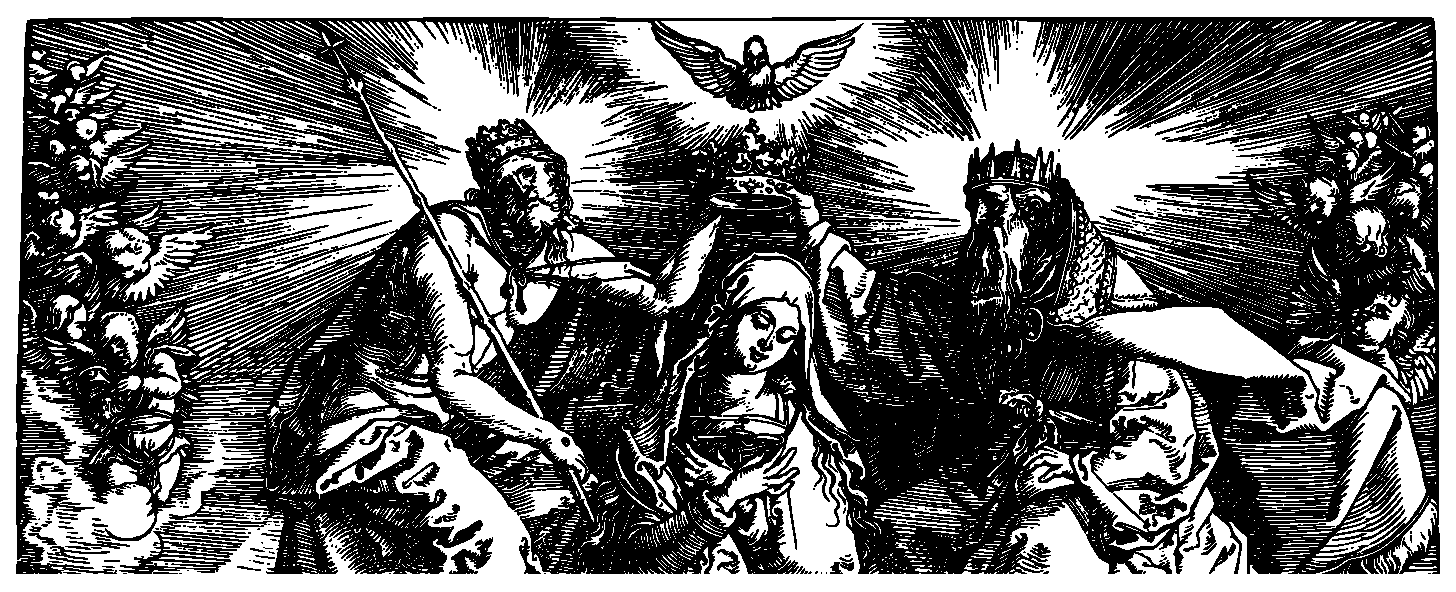
\includegraphics[width=103.001mm,height=40.314mm]{tailpiece/Assumption.eps}
  \end{figure}
  
%MANUAL ADJUSTMENT:
\clearpage
\festival{First Class Double, Common Octave}{15 August}{Assumption of the Blessed Virgin Mary}
\feastday{Assumption B.V.M.}
\feastdate{15}{August}

\introit
\lett{R}{ejoice} we all in the Lord, keeping feast day in honour of the blessed Virgin Mary: in whose Assumption the Angels rejoice and glorify the Son of God. \textit{Ps.} My heart is inditing of a good matter: I speak of the things which I have made unto the King.

\collect
\lett{W}{e} beseech thee, O Lord, let us be continually aided by the sacred feast of this day, whereon the holy Mother of God underwent death in this world, and yet could not be holden by the chains of death: who did bring forth thy Son our Lord. Who liveth.

\readingcitation{Epistle}{Ecclesiasticus 24:7}
\lett{W}{ith} all these I sought rest; And in whose inheritance shall I lodge? Then the Creator of all things gave me a commandment; And he that created me made my tabernacle to rest, And said, Let thy tabernacle be in Jacob, And thine inheritance in Israel. He created me from the beginning before the world; And to the end I shall not fail. In the holy tabernacle I ministered before him; And so was I established in Sion. In the beloved city likewise he gave me rest; And in Jerusalem was my authority. And I took root in a people that was glorified, Even in the portion of the Lord’s own inheritance. I was exalted like a cedar in Libanus, And as a cypress tree on the mountains of Hermon. I was exalted like a palm tree on the sea shore, And as rose plants in Jericho, And as a fair olive tree in the plain; And I was exalted as a plane tree. As cinnamon and aspalathus, I have given a scent of perfumes; And as choice myrrh, I spread abroad a pleasant odour.

\gradall{Because of the word of truth, of meekness, and righteousness, and thy right hand shall teach thee terrible things. ℣. Hearken, O daughter, and consider, incline thine ear: so shall the King have pleasure in thy beauty.}{Alleluia, alleluia. ℣. This day the Virgin Mary entered heaven: rejoice, for she reigneth with Christ for ever. Alleluia.}

%MANUAL ADJUSTMENT:
\clearpage
\subsubsection{Sequence}

\vspace{-0.5\baselineskip}

\begin{multicols}{2}
\begin{hangparas}{1.25em}{1}
From our first Mother Eva's sickly branch

Mary the blooming rose proceeded forth;

Bright as amidst the stars the Morning Star,

And fair in beauty as the moon she came;

\vspace{0.5\baselineskip}

Sweet beyond balsam, ointments, frankincense;

As violet glowing, dewy as the rose,

White as the lily, she who was preferred

To bear the highest Father's holy Child,

That of a Virgin's flesh immaculate

He might upon him take flesh hallowed.

Great Gabriel brings the message of new joy,

Th' arising of the eternal King on earth,

\vspace{0.5\baselineskip}

And to his Mother thus gives salutation:

Blessed art thou, Queen of the universe!

Blessed art thou, Queen of the universe!

Blessed art thou, Queen of the universe!

Thou shalt bring forth the Everlasting King.

She answered, How can I fruitful be,

\vspace{0.5\baselineskip}

Seeing a man I know not, from my birth

Ever a Virgin chaste continuing?

Fear not (the Angel answered), upon thee,

Chaste as thou art, the Holy Ghost shall come,

\vspace{0.5\baselineskip}

Whereby thou shalt bear God and Man in one.

O truly holy, truly to be loved!

Of whom redemption hath for us arisen,

Salvation of the world, and our true life.

\vspace{0.5\baselineskip}

Mother of God, accept our prayers this day,

Whereon to heaven's portals thou wast borne.

Dear to the Father, Jesus' Mother pure,

The Holy Spirit's temple thou wast made.

\vspace{0.5\baselineskip}

Fair Spouse of God, thou Christ the King hast borne:

Lady thou art in heaven and in earth.

This day hosts met thee from the court of heaven,

And to the starry palace led thee up.

\vspace{0.5\baselineskip}

Jesus himself, to welcome thee his Mother,

Came with the angels forth, and set thee up

With him for ever in his Father's seat.

With God now reigning, mercifully pardon

\vspace{0.5\baselineskip}

Our evil deeds, and ask for us all good.

O gracious Mediatrix, next to God

Our only hope, commend us to thy Son,

That we in highest heaven may Alleluias sing.
\end{hangparas}
\end{multicols}

\readingcitation{Gospel}{Luke 10:38}
\lett{A}{t that time:} It came to pass, as they went, that Jesus entered into a certain village: and a certain woman named Martha received him into her house. And she had a sister called Mary, which also sat at Jesus' feet, and heard his word. But Martha was cumbered about much serving, and came to him, and said, Lord, dost thou not care that my sister hath left me to serve alone? bid her therefore that she help me. And Jesus answered and said unto her, Martha, Martha, thou art careful and troubled about many things: but one thing is needful: and Mary hath chosen that good part, which shall not be taken away from her.

\offertory{Full of grace are thy lips, because God hath blessed thee for ever.}

\secret
\lett{W}{e} beseech thee, O Lord, that the prayers of the Blessed Mother of God may make our gifts acceptable to thee, that albeit we know her to have departed this life in respect of this flesh we may perceive her prayers for us continually in the glory of heaven. Through.

\communion{Blessed is the womb of the Virgin Mary, which bare the Son of the everlasting Father.}

\postcommunion
\lett{W}{e} that have partaken of thy heavenly table implore thy mercy, O Lord our God, that we who keep the feast of the Mother of God may at her intercession be delivered from all evils which beset us. Through.

\begin{rubric}
    Within the Octave, Mass is said as on the Feast. And the \nth{2} Prayers are \blackrubric{of the Holy Ghost} (p. \pageref{SPHolyGhost}) \& \nth{3} \blackrubric{Against the Persecutors of the Church} (p. \pageref{SPAgainst}) or \blackrubric{for the Chief Bishop} (p. \pageref{SPChiefBishop}).
\end{rubric}

\begin{rubric}
    The following Alleluia is said daily, except on the Sunday in the Octave and the Octave Day.
\end{rubric}
\alleluia{Alleluia, alleluia. ℣. Mary is taken up into heaven: angels rejoice, praise, and bless the Lord.}


%MANUAL ADJUSTMENT:
\clearpage
\festival{Second Class Double}{16 August}{St. Joachim, Father of the Blessed Virgin Mary}
\feastday{St. Joachim}
\feastdate{16}{August}

\introit
\lett{H}{e} hath dispersed abroad, and given to the poor his righteousness remaineth for ever: his horn shall be exalted with honour. \textit{Ps.} Blessed is the man that feareth the Lord he hath great delight in his commandments.

\collect
\lett{O}{God,} who from amongst all thy Saints didst choose blessed Joachim to be the father of the Mother of thy Son: grant, we beseech thee; that we who venerate his festival may also continually perceive his advocacy. Through the same.

\readingcitation{Epistle}{Ecclesiasticus 31:8}
\lett{B}{lessed} is the rich that is found without blemish, And that goeth not after gold. Who is he? and we will call him blessed: For wonderful things hath he done among his people. Who hath been tried thereby, and found perfect? Then let him glory. Who hath had the power to transgress, and hath not transgressed? And to do evil, and hath not done it? His goods shall be made sure, And the congregation shall declare his alms.

\gradall{He hath dispersed abroad, and given to the poor: his righteousness remaineth for ever. ℣. His seed shall be mighty upon earth: the generation of the faithful shall be blessed.}{Alleluia, alleluia. ℣. Joachim, spouse of Saint Anne, of the gracious Virgin the father, here to thy servants bring safety and aid from on high. Alleluia.}

\readingcitation{Gospel}{Matthew 1:1}
\lett{T}{he} book of the generation of Jesus Christ, the son of David, the son of Abraham. Abraham begat Isaac; and Isaac begat Jacob; and Jacob begat Judas and his brethren; And Judas begat Phares and Zara of Thamar; and Phares begat Esrom; and Esrom begat Aram; And Aram begat Aminadab; and Aminadab begat Naasson; and Naasson begat Salmon; And Salmon begat Booz of Rachab; and Booz begat Obed of Ruth; and Obed begat Jesse; And Jesse begat David the king; and David the king begat Solomon of her that had been the wife of Urias; And Solomon begat Roboam; and Roboam begat Abia; and Abia begat Asa; And Asa begat Josaphat; and Josaphat begat Joram; and Joram begat Ozias; And Ozias begat Joatham; and Joatham begat Achaz; and Achaz begat Ezekias; And Ezekias begat Manasses; and Manasses begat Amon; and Amon begat Josias; And Josias begat Jechonias and his brethren, about the time they were carried away to Babylon: And after they were brought to Babylon, Jechonias begat Salathiel; and Salathiel begat Zorobabel; And Zorobabel begat Abiud; and Abiud begat Eliakim; and Eliakim begat Azor; And Azor begat Sadoc; and Sadoc begat Achim; and Achim begat Eliud; And Eliud begat Eleazar; and Eleazar begat Matthan; and Matthan begat Jacob; And Jacob begat Joseph the husband of Mary, of whom was born Jesus, who is called Christ.

\offertory{Thou hast crowned him with glory and worship: and hast made him to have dominion of the works of thy hands, O Lord.}

\secret
\lett{R}{eceive,} most merciful God, the sacrifice which we offer to thy Majesty, in honour of the holy Patriarch Joachim, father of the Virgin Mary: and grant that, he with his wife and their most blessed offspring interceding for us, we may be counted worthy to receive perfect remission of sins and everlasting glory. Through the same.

\communion{A faithful and wise servant, whom the lord hath made ruler over his household: to give them their portion of meat in due season.}

\postcommunion
\lett{W}{e} beseech thee, Almighty God: that through these sacraments which we have received, with the pleading of the merits and prayers of blessed Joachim, father of the Mother of thy beloved Son Jesus Christ our Lord, we may be found worthy to be made partakers of thy grace in this life and of eternal glory in the life to come. Through the same.


\festival{Simple}{17 August}{Octave Day of St. Lawrence}
\feastday{{St. Lawrence Octave Day}}
\feastdate{17}{August}

\introit
\lett{T}{hou} hast proved and visited mine heart, O Lord, in the night-season: thou hast tried me with fire, and hast found no wickedness in me. \textit{Ps.} Hear the right, O Lord: consider my complaint.

\collect
\lett{S}{tir} up, O Lord, in thy Church that Spirit whom the blessed Levite Lawrence served: that we, being filled with the same, may study to love that which he loved, and to perform in deed that which he taught. Through . . . in the unity of the same Holy Spirit.

\readingcitation{Epistle}{2 Corinthians 9:6}
\lett{B}{rethren:} He which soweth sparingly shall reap also sparingly; and he which soweth bountifully shall reap also bountifully. Every man according as he purposeth in his heart, so let him give; not grudgingly, or of necessity: for God loveth a cheerful giver. And God is able to make all grace abound toward you; that ye, always having all sufficiency in all things, may abound to every good work: (As it is written, He hath dispersed abroad; he hath given to the poor: his righteousness remaineth for ever. Now he that ministereth seed to the sower both minister bread for your food, and multiply your seed sown, and increase the fruits of your righteousness;)

\gradall{Thou hast crowned him with glory and worship, O Lord. ℣. And hast made him to have dominion of the works of thy hands.}{Alleluia, alleluia. ℣. The Levite Lawrence wrought a good work: who by the sign of the cross gave light to the blind. Alleluia.}

\readingcitation{Gospel}{John 12:24}
\lett{A}{t that time:} Jesus said unto his disciples: Verily, verily, I say unto you, Except a corn of wheat fall into the ground and die, it abideth alone: but if it die, it bringeth forth much fruit. He that loveth his life shall lose it; and he that hateth his life in this world shall keep it unto life eternal. If any man serve me, let him follow me; and where I am, there shall also my servant be: if any man serve me, him will my Father honour.

\offertory{The just shall rejoice in thy strength, O Lord: exceeding glad shall he be of thy salvation: thou hast given him his heart's desire.}

\secret
\lett{O}{Lord,} we beseech thee, let the holy prayer of blessed Lawrence commend the sacrifices unto thee: that it may be rendered acceptable by the merits of him in whose honour it is solemnly offered forth. Through.

\communion{He that will come after me, let him deny himself, and take up his cross, and follow me.}

\postcommunion
\lett{W}{e} humbly beseech thee, Almighty God: that we, whom thou hast fulfilled with heavenly gifts, may, at the intercession of blessed Lawrence thy Martyr, be defended by thy continual protection. Through.


\subbymemorial{18 August}{St. Helen}
\feastday{{St. Helen}}
\feastdate{18}{August}

\introit
\lett{B}{ut} God forbid that I should glory, save in the Cross of our Lord Jesus Christ: by whom the world is crucified unto me, and I unto the world. \textit{Ps.} Thy rod and thy staff comfort me.

\collect
\lett{O}{Lord} Jesu Christ, who didst reveal unto blessed Helen the place where thy Cross lay hid, that through her thou mightest enrich thy Church with this precious treasure: grant unto us at her intercession; that by the ransom of the life-giving tree we may attain unto the rewards of everlasting life. Who livest.

\readingcitation{Epistle}{Proverbs 31:10}
\lett{W}{ho} can find a virtuous woman? for her price is far above rubies. The heart of her husband doth safely trust in her, so that he shall have no need of spoil. She will do him good and not evil all the days of her life. She seeketh wool, and flax, and worketh willingly with her hands. She is like the merchants' ships; she bringeth her food from afar. She riseth also while it is yet night, and giveth meat to her household, and a portion to her maidens. She considereth a field, and buyeth it: with the fruit of her hands she planteth a vineyard. She girdeth her loins with strength, and strengtheneth her arms. She perceiveth that her merchandise is good: her candle goeth not out by night. She layeth her hands to the spindle, and her hands hold the distaff. She stretcheth out her hand to the poor; yea, she reacheth forth her hands to the needy. She is not afraid of the snow for her household: for all her household are clothed with scarlet. She maketh herself coverings of tapestry; her clothing is silk and purple. Her husband is known in the gates, when he sitteth among the elders of the land. She maketh fine linen, and selleth it; and delivereth girdles unto the merchant. Strength and honour are her clothing; and she shall rejoice in time to come. She openeth her mouth with wisdom; and in her tongue is the law of kindness. She looketh well to the ways of her household, and eateth not the bread of idleness. Her children arise up, and call her blessed; her husband also, and he praiseth her. Many daughters have done virtuously, but thou excellest them all. Favour is deceitful, and beauty is vain: but a woman that feareth the \divineName{Lord}, she shall be praised. Give her of the fruit of her hands; and let her own works praise her in the gates.

\gradall{Like as the rich also among the people shall make their supplication before thee. Kings' daughters were among thy honourable women. ℣. She shall be brought unto the King in raiment of needle-work: the virgins that be her fellows shall bear her company, and shall be brought unto thee. With joy and gladness shall they be brought: and shall enter into the King's palace.}{Alleluia, alleluia. ℣. He hath dispersed abroad, and given to the poor : and his righteousness remaineth for ever. Alleluia.}

\readingcitation{Gospel}{Matthew 13:44}
\lett{A}{t that time:} Jesus spake this parable to his disciples: The kingdom of heaven is like unto treasure hid in a field; the which when a man hath found, he hideth, and for joy thereof goeth and selleth all that he hath, and buyeth that field. Again, the kingdom of heaven is like unto a merchant man, seeking goodly pearls: Who, when he had found one pearl of great price, went and sold all that he had, and bought it. Again, the kingdom of heaven is like unto a net, that was cast into the sea, and gathered of every kind: Which, when it was full, they drew to shore, and sat down, and gathered the good into vessels, but cast the bad away. So shall it be at the end of the world: the angels shall come forth, and sever the wicked from among the just, And shall cast them into the furnace of fire: there shall be wailing and gnashing of teeth. Jesus saith unto them, Have ye understood all these things? They say unto him, Yea, Lord. Then said he unto them, Therefore every scribe which is instructed unto the kingdom of heaven is like unto a man that is an householder, which bringeth forth out of his treasure things new and old.

\offertory{For I determined not to know any thing, save Jesus Christ, and him crucified.}

\secret
\lett{T}{hrough} these sacred mysteries vouchsafe unto us, O Lord: that as in thy mercy thou didst grant unto blessed Helen ever to carry thy Son crucified in her heart; so we may likewise continually hear him in our hearts. Who liveth and reigneth with thee.

\communion{I will go up to the palm tree, I will take hold of the boughs thereof.}

\postcommunion
\lett{G}{rant} unto us, O merciful God: that we who have been refreshed by the benefits of thy life-giving Cross on earth; may through the intercession of blessed Helen attain unto the eternal fruition of the same in heaven. Who livest.


\subbymemorial{18 August}{St. Agapitus}
\feastday{{St. Agapitus}}
\feastdate{18}{August}

\begin{rubric}
	The Second Common of a Martyr not a Bishop (p. \pageref{CommonMartyrNotBishopII}).
\end{rubric}

\collect
\lett{O}{Lord,} let thy Church trust with gladness in the advocacy of thy blessed Martyr Agapitus: that by his glorious prayers she may continue in devotion, and abide in safety. Through.

\readingcitation{Gospel}{John 12:24}
\lett{A}{t that time:} Jesus said unto his disciples: Verily, verily, I say unto you, Except a corn of wheat fall into the ground and die, it abideth alone: but if it die, it bringeth forth much fruit. He that loveth his life shall lose it; and he that hateth his life in this world shall keep it unto life eternal. If any man serve me, let him follow me; and where I am, there shall also my servant be: if any man serve me, him will my Father honour.

\secret
\lett{R}{eceive,} O Lord, the gifts which we offer on the solemnity of him, through whose advocacy we trust to be delivered. Through.

\lettspace

\postcommunion
\lett{O}{Lord,} who hast satisfied thy family with sacred gifts: we beseech thee; that we may at all times be comforted by the intercession of him whose festival we celebrate. Through.


\festival{Greater Double}{22 August}{Octave Day of the Assumption of the Blessed Virgin Mary}
\feastday{{Assumption Octave Day}}
\feastdate{22}{August}

\begin{rubric}
	Mass as on the Feast with Commemoration \blackrubric{of Sts. Timothy, Hippolytus, \& Symphorian,} as in the following Mass.
\end{rubric}
\begin{rubric}
	If today be Saturday, \blackrubric{the anticipated Vigil of St. Bartholomew} is kept, as is noted on the following day.
\end{rubric}


\subbymemorial{22 August}{Sts. Timothy, Hippolytus, and Symphorian}
\feastday{{Sts. Timothy \&c.}}
\feastdate{22}{August}

\begin{rubric}
	The Third Common of Many Martyrs (p. \pageref{CommonMartyrsIII}).
\end{rubric}

\collect
\lett{W}{e} beseech thee, O Lord, graciously to impart unto us thy help: and, at the intercession of thy blessed Martyrs Timothy, Hippolytus, and Symphorian, stretch forth upon us the right hand of thy mercy. Through.

\secret
\lett{G}{rant,} O Lord, that like as thy dedicated people do acknowledge that in tribulation they have been succoured by the merits of thy Saints: so this oblation, which they offer unto thee in honour of the same, may be acceptable in thy sight. Through.

\postcommunion
\lett{O}{Lord} our God, who hast fulfilled us with the bounty of thy heavenly gift: we beseech thee, that, at the intercession of thy holy Martyrs, Timothy, Hippolytus, and Symphorian, we may ever live by the partaking of the same. Through.


%MANUAL ADJUSTMENT:
\clearpage
\festival{Vigil}{23 August}{Vigil of St. Bartholomew}
\feastday{{St. Bartholomew Vigil}}
\feastdate{23}{August}

\begin{rubric}
	The Common of the Vigil of Apostles (p. \pageref{CommonVigilApostles}).
\end{rubric}
\begin{rubric}
	Commemoration \blackrubric{of the Saints} (p. \pageref{SPSaints}) \& \blackrubric{ad libitum}.
\end{rubric}


\festival{Second Class Double}{24 August}{St. Bartholomew}
\feastday{St. Bartholomew}
\feastdate{24}{August}

\introit
\lett{R}{ight} honourable are thy friends unto me, O God: right well is their princedom established. \textit{Ps.} O Lord, thou hast searched me out, and known me: thou knowest my down-sitting and mine up-rising.

\collect
\lett{O}{Almighty} and Everlasting God, who didst give to thine Apostle Bartholomew grace truly to believe and to preach thy Word; Grant, we beseech thee, unto thy Church to love that Word which he believed, and both to preach and receive the same. Through.

\readingcitation{Epistle}{Acts 5:12}
\lett{I}{n those days:} By the hands of the apostles were many signs and wonders wrought among the people; (and they were all with one accord in Solomon's porch. And of the rest durst no man join himself to them: but the people magnified them. And believers were the more added to the Lord, multitudes both of men and women.) Insomuch that they brought forth the sick into the streets, and laid them on beds and couches, that at the least the shadow of Peter passing by might overshadow some of them. There came also a multitude out of the cities round about unto Jerusalem, bringing sick folks, and them which were vexed with unclean spirits: and they were healed every one.

\gradall{Thou shalt make them princes in all lands: they shall remember thy name, O Lord. ℣. Instead of thy fathers thou shalt have children: therefore shall the people give thanks unto thee.}{Alleluia, alleluia. ℣. The glorious company of the Apostles praise thee, O Lord. Alleluia.}

\readingcitation{Gospel}{Luke 22:24}
\lett{A}{t that time:} There was a strife among the disciples, which of them should be accounted the greatest. And he said unto them, The kings of the Gentiles exercise lordship over them; and they that exercise authority upon them are called benefactors. But ye shall not be so: but he that is greatest among you, let him be as the younger; and he that is chief, as he that doth serve. For whether is greater, he that sitteth at meat, or he that serveth? is not he that sitteth at meat? but I am among you as he that serveth. Ye are they which have continued with me in my temptations. And I appoint unto you a kingdom, as my Father hath appointed unto me; That ye may eat and drink at my table in my kingdom, and sit on thrones judging the twelve tribes of Israel.

\offertory{Right honourable are thy friends unto me, O God: right well is their princedom established.}

\secret
\lett{W}{e} beseech thee, O Lord, that we, who celebrate the festival of thy blessed Apostle Bartholomew: may, by the succour of him in whose honour we offer thee these sacrifices of praise, receive thy benefits. Through

\communion{Ye which have followed me shall sit upon thrones, judging the twelve tribes of Israel, saith the Lord.}

\postcommunion
\lett{O}{Lord,} through whom we have received the pledge of eternal redemption: we beseech thee; that at the intercession of blessed Bartholomew, thine Apostle, it may avail for our succour both in this life and that which is to come. Through.


\subbymemorial{26 August}{St. Zephyrinus}
\feastday{{St. Zephyrinus}}
\feastdate{26}{August}

\begin{rubric}
	The Second Common of a Martyr Bishop out of Eastertide (p. \pageref{CommonMartyrBishopII}).
\end{rubric}

\collect
\lett{G}{rant,} we beseech thee, Almighty God: that we who rejoice in the merits of blessed Zephyrinus, thy Martyr and Bishop, may be instructed by his example. Through.

\secret
\lett{S}{anctify,} O Lord, the gifts which we dedicate to thee: that at the intercession of blessed Zephyrinus thy Martyr and Bishop they may obtain for us thy gracious favour. Through.

\postcommunion
\lett{M}{ay} this communion, O Lord, cleanse us from guilt: and, at the intercession of blessed Zephyrinus, thy Martyr and Bishop, make us partakers of thy heavenly healing. Through.


\festival{Greater Double}{28 August}{St. Augustine of Hippo}
\feastday{{St. Augustine Hippo}}
\feastdate{28}{August}

\begin{rubric}
	The Common of Doctors (p. \pageref{CommonDoctors}).
\end{rubric}

\introit
\lett{I}{n} the midst of the Church he opened his mouth: and the Lord filled him with the spirit of wisdom and of understanding: he clothed him with a robe of glory. \textit{Ps.} It is a good thing to give thanks unto the Lord: and to sing praises unto thy name, O most Highest.

\collect
\lett{A}{ssist} us, Almighty God, in these our supplications: that as thou dost suffer us to put our trust and confidence in thy mercy, so, at the intercession of blessed Augustine thy Confessor and Bishop, thou wouldest graciously vouchsafe unto us the wonted effects of thy compassion. Through.

\begin{rubric}
    Commemoration \blackrubric{of St. Hermes} (p. \pageref{HermesCollect}).
\end{rubric}

\gradall{The mouth of the righteous is exercised in wisdom, and his tongue will be talking judgment. ℣. The law of his God is in his heart: and his goings shall not slide.}{Alleluia, alleluia. ℣. I have found David my servant, with my holy oil have I anointed him. Alleluia.}

\offertory{The righteous shall flourish like a palm-tree: and shall spread abroad like a cedar in Libanus.}

\secret
\lett{M}{ay} the devout prayers of thy Bishop and Doctor, Saint Augustine, never fail to succour us, O Lord: that they may render our oblations acceptable in thy sight; and may ever obtain for us thy merciful pardon. Through.

\begin{rubric}
    Commemoration \blackrubric{of St. Hermes} (p. \pageref{HermesSecret}).
\end{rubric}

\communion{A faithful and wise servant, whom the lord hath made ruler over his household: to give them their portion of meat in due season.}

\postcommunion
\lett{W}{e} beseech thee, O Lord, that blessed Augustine, thy Bishop and illustrious Doctor, may stand before thee as our advocate: that these thy sacrifices may avail for our salvation. Through.

\begin{rubric}
    Commemoration \blackrubric{of St. Hermes} (p. \pageref{HermesPostcommunion}).
\end{rubric}


\subbymemorial{28 August}{St. Hermes}
\feastday{{St. Hermes}}
\feastdate{28}{August}

\begin{rubric}
	The Second Common of a Martyr not a Bishop (p. \pageref{CommonMartyrNotBishopII}).
\end{rubric}

\collect\label{HermesCollect}
\lett{O}{God,} who didst strengthen blessed Hermes thy Martyr with the virtue of constancy in his passion: Grant unto us by his example; to despise for love of thee the prosperity of the world, and to fear none of its adversities. Through.

\secret\label{HermesSecret}
\lett{W}{e} offer unto thee, O Lord, this sacrifice of praise in commemoration of thy Saints: grant, we beseech thee; that as it hath bestowed glory on them, so may it avail for our salvation. Through.

\postcommunion\label{HermesPostcommunion}
\lett{O}{Lord,} who hast fulfilled us with thy heavenly benediction, we beseech thy mercy: that, at the intercession of thy blessed Martyr Hermes, this service of our lowliness may avail for the comforting of our souls. Through.


%MANUAL ADJUSTMENT:
\clearpage
\festival{Greater Double}{29 August}{Decollation of St. John Baptist}
\feastday{Decollation}
\feastdate{29}{August}

\introit
\lett{I}{will} speak of thy testimonies, even before kings, and will not be ashamed: and my delight shall be in thy commandments, which I have loved exceedingly. \textit{Ps.} It is a good thing to give thanks unto the Lord: and to sing praises unto thy name, O most Highest.

\collect
\lett{W}{e} beseech thee, O Lord: that the venerable festival of thy Forerunner and Martyr, Saint John Baptist, may effectually bestow upon us thy succour unto our salvation. Who livest.
\begin{rubric}
	 Commemoration \blackrubric{of St. Sabina,} from the Common of a Martyress not a Virgin (p. \pageref{CommonMartyrNotVirgin}).
\end{rubric}

\readingcitation{Epistle}{Jeremiah 1:17}
\lett{I}{n those days:} The word of the Lord came unto me, saying: Gird up thy loins, and arise, and speak unto Judah all that I command thee: be not dismayed at their faces, lest I confound thee before them. For, behold, I have made thee this day a defenced city, and an iron pillar, and brasen walls against the whole land, against the kings of Judah, against the princes thereof, against the priests thereof, and against the people of the land. And they shall fight against thee; but they shall not prevail against thee; for I am with thee, saith the Lord, to deliver thee.

\gradall{The righteous shall flourish like a palm-tree: and shall spread abroad like a cedar in Libanus in the house of the Lord. ℣. To tell of thy loving-kindness early in the morning, and of thy truth in the night-season.}{Alleluia, alleluia. ℣. The righteous shall grow as the lily: and shall flourish for ever before the Lord. Alleluia.}

\readingcitation{Gospel}{Mark 6:17}
\lett{A}{t that time:} Herod sent forth and laid hold upon John, and bound him in prison for Herodias' sake, his brother Philip’s wife: for he had married her. For John had said unto Herod, It is not lawful for thee to have thy brother’s wife. Therefore Herodias had a quarrel against him, and would have killed him; but she could not: for Herod feared John, knowing that he was a just man and an holy, and observed him; and when he heard him, he did many things, and heard him gladly. And when a convenient day was come, that Herod on his birthday made a supper to his lords, high captains, and chief estates of Galilee; and when the daughter of the said Herodias came in, and danced, and pleased Herod and them that sat with him, the king said unto the damsel, Ask of me whatsoever thou wilt, and I will give it thee. And he sware unto her, Whatsoever thou shalt ask of me, I will give it thee, unto the half of my kingdom. And she went forth, and said unto her mother, What shall I ask? And she said, The head of John the Baptist. And she came in straightway with haste unto the king, and asked, saying, I will that thou give me by and by in a charger the head of John the Baptist. And the king was exceeding sorry; yet for his oath’s sake, and for their sakes which sat with him, he would not reject her. And immediately the king sent an executioner, and commanded his head to be brought: and he went and beheaded him in the prison, and brought his head in a charger, and gave it to the damsel: and the damsel gave it to her mother. And when his disciples heard of it, they came and took up his corpse, and laid it in a tomb.

\offertory{The just shall rejoice in thy strength, O Lord, exceeding glad shall he be of thy salvation: thou hast given him his heart's desire.}

\secret
\lett{W}{e} beseech thee, O Lord, that the gifts which we offer unto thee for the passion of thy holy Martyr John Baptist: may through his intercession be profitable for our salvation. Through.
\begin{rubric}
	 Commemoration \blackrubric{of St. Sabina,} from the Common of a Martyress not a Virgin (p. \pageref{CommonMartyrNotVirgin}).
\end{rubric}

\communion{Thou hast set, O Lord, a crown of pure gold upon his head.}

\postcommunion
\lett{L}{et} the solemnity, of Saint John Baptist enable us, O Lord: both to reverence those things which are signified in the wondrous sacraments which we have received, and to rejoice abundantly in the fruits that they bring forth in us. Through.
\begin{rubric}
	 Commemoration \blackrubric{of St. Sabina,} from the Common of a Martyress not a Virgin (p. \pageref{CommonMartyrNotVirgin}).
\end{rubric}


%MANUAL ADJUSTMENT:
\clearpage
\subbymemorial{29 August}{St. Sabina}
\feastday{{St. Sabina}}
\feastdate{29}{August}

\begin{rubric}
	The Common of a Martyress not a Virgin (p. \pageref{CommonMartyrNotVirgin}).
\end{rubric}


\subbymemorial{30 August}{Sts. Felix and Adauctus}
\feastday{{Sts. Felix \& Adauctus}}
\feastdate{30}{August}

\introit
\lett{L}{et} the people tell of the wisdom of the Saints, and let the church shew forth their praise: their names shall live for evermore. \textit{Ps.} Rejoice in the Lord, O ye righteous: for it becometh well the just to be thankful.

%MANUAL ADJUSTMENT:
\vspace{-0.25\baselineskip}

\collect

%MANUAL ADJUSTMENT:
\vspace{-0.1\baselineskip}

\lett{O}{Lord,} we humbly entreat thy Majesty: that, like as thou dost continually gladden us with the commemoration of thy Saints; so thou wouldest evermore defend us with their supplication. Through.

\begin{rubric}
	The Epistle is the third additional Epistle from the Third Common of Many Martyrs (p. \pageref{Wisdom1017}).
\end{rubric}

\gradall{The souls of the just are in the hand of God, and there shall no torment of malice touch them. ℣. In the eyes of the unwise they seemed to die: but they are in peace.}{Alleluia, alleluia. ℣. The righteous shall shine forth, and run to and fro like sparks among the stubble for ever. Alleluia.}

\begin{rubric}
	The Gospel is the fifth additional Gospel from the Third Common of Many Martyrs (p. \pageref{Luke1016}).
\end{rubric}

\offertory{Be glad, O ye righteous, and rejoice in the Lord: and be joyful, all ye that are true of heart.}

%MANUAL ADJUSTMENT:
\vspace{-0.35\baselineskip}

\secret

%MANUAL ADJUSTMENT:
\vspace{-0.1\baselineskip}

\lett{L}{ook} down, O Lord, upon the sacrifices of thy people: that, as with devout hearts they celebrate them to the honour of thy Saints, so they may perceive them to be profitable to their salvation. Through.

\communion{What I tell you in darkness, that speak ye in light, saith the Lord: and what ye hear in the ear, that preach ye upon the housetops.}

%MANUAL ADJUSTMENT:
\vspace{-0.15\baselineskip}

\postcommunion

%MANUAL ADJUSTMENT:
\vspace{-0.05\baselineskip}

\lett{W}{e} beseech thee, O Lord: that we, being filled with the sacred gifts; may at the intercession of thy Saints ever continue in thanksgiving for the same. Through.


%MANUAL ADJUSTMENT:
\clearpage
\subbymemorial{31 August}{St. Aidan of Lindisfarne}
\feastday{{St. Aidan Lindisfarne}}
\feastdate{31}{August}

\begin{rubric}
	The First Common of a Confessor Bishop (p. \pageref{CommonConfessorBishopI}).
\end{rubric}


\subbymemorial{1 September}{St. Giles}
\feastday{{St. Giles}}
\feastdate{1}{September}

\begin{rubric}
	The Common of Abbots (p. \pageref{CommonAbbots}).
\end{rubric}


\subbymemorial{1 September}{Twelve Holy Brothers}
\feastday{{12 Holy Brothers}}
\feastdate{1}{September}

\introit
\lett{T}{he} just cry, and the Lord heareth them: and delivereth them out of all their troubles. \textit{Ps.} I will alway give thanks unto the Lord; his praise shall ever be in my mouth.

\collect
\lett{O}{Lord,} let the crown of the brethren thy Martyrs, cause us to rejoice: that we may thereby be strengthened and increased in our faith; and comforted by their manifold intercession. Through.

\begin{rubric}
	The Epistle is the fifth additional Epistle of the Third Common of Many Martyrs (p. \pageref{Hebrews1133}).
\end{rubric}

\gradall{Behold, how good and joyful a thing it is, brethren, to dwell together in unity! ℣. It is like the precious ointment upon the head, that ran down unto the beard, even unto Aaron's beard.}{Alleluia, alleluia. ℣. This is the true brotherhood which overcame the wickedness of the world: which followed Christ, gaining heaven's glorious realms. Alleluia.}

\begin{rubric}
	The Gospel is from the Third Common of Many Martyrs (p. \pageref{CommonMartyrsIIGospel}).
\end{rubric}

\offertory{Be glad, O ye righteous, and rejoice in the Lord: and be joyful, all ye that are true of heart.}

\secret
\lett{G}{rant,} O Lord, that we may with devout hearts celebrate thy mysteries in honour of thy holy Martyrs: and thereby obtain an increase both of protection and joy. Through.

\communion{Whosoever shall do the will of my Father which is in heaven: the same is my brother, and sister, and mother, saith the Lord.}

\postcommunion
\lett{G}{rant,} we beseech thee, Almighty God: that growing in virtue we may follow the faith of them whose memory we recall by the partaking of this sacrament. Through.


\subbymemorial{2 August}{St. Stephen of Hungary}
\feastday{{St. Stephen Hungary}}
\feastdate{2}{September}

\begin{rubric}
	The First Common of Confessor not Bishop (p. \pageref{CommonConfessorNotBishopI}).
\end{rubric}

\collect
\lett{G}{rant,} we beseech thee, Almighty God unto thy Church: that as thy blessed Confessor Stephen, while he reigned on earth, did spread abroad her faith, so she may be found worthy to have him for her glorious defender in the heavens. Through.

\begin{rubric}
	The Gospel is the additional Gospel from the Second Common of a Confessor not a Bishop (p. \pageref{Luke1912}).
\end{rubric}

\secret
\lett{A}{lmighty} God, look upon the sacrifices which we offer: and grant; that we, who celebrate the mysteries of the Passion of the Lord, may imitate that which we perform. Through the same.

\postcommunion
\lett{G}{rant,} we beseech thee, Almighty God: that, as thy blessed Confessor Stephen, for the propagation of thy faith, was counted worthy to pass from an earthly kingdom to the glory of the heavenly realm; so we may imitate his faith with due devotion. Through.


\festival{Double}{4 September}{St. Gorazde of Prague}
\feastday{{St. Gorazde Prague}}
\feastdate{4}{September}

\begin{rubric}
	The Second Common of a Martyr Bishop (p. \pageref{CommonMartyrBishopII}).
\end{rubric}


%MANUAL ADJUSTMENT:
\clearpage
\festival{Second Class Double, Simple Octave}{8 September}{Nativity of the Blessed Virgin Mary}
\feastday{Nativity B.V.M.}
\feastdate{8}{September}

\introit
\lett{H}{ail,} O Mother most holy, who in childbirth didst bring forth the Monarch: him who o'er heaven and earth reigneth for ever and ever. \textit{Ps.} My heart is inditing of a good matter: I speak of the things which I have made unto the King.

\collect
\lett{W}{e} beseech thee, O Lord, to grant unto us thy servants the gift of heavenly grace: that as the childbearing of the blessed Virgin was unto us the beginning of salvation; so the devout observance of her Nativity may bestow an increase of peace. Through.

\readingcitation{Epistle}{Proverbs 8:22}
\lett{T}{he} \textsc{Lord} possessed me in the beginning of his way, before his works of old. I was set up from everlasting, from the beginning, or ever the earth was. When there were no depths, I was brought forth; when there were no fountains abounding with water. Before the mountains were settled, before the hills was I brought forth: While as yet he had not made the earth, nor the fields, nor the highest part of the dust of the world. When he prepared the heavens, I was there: when he set a compass upon the face of the depth: When he established the clouds above: when he strengthened the fountains of the deep: When he gave to the sea his decree, that the waters should not pass his commandment: when he appointed the foundations of the earth: Then I was by him, as one brought up with him: and I was daily his delight, rejoicing always before him; Rejoicing in the habitable part of his earth; and my delights were with the sons of men. Now therefore hearken unto me, O ye children: for blessed are they that keep my ways. Hear instruction, and be wise, and refuse it not. Blessed is the man that heareth me, watching daily at my gates, waiting at the posts of my doors. For whoso findeth me findeth life, and shall obtain favour of the \textsc{Lord}.

\gradall{Blessed and venerable art thou, O Virgin Mary: who without spot wast found Mother of the Saviour. ℣. Virgin, Mother of God, he, whom the whole world containeth not, being made man lay hid in thy womb.}{Alleluia, alleluia, ℣. Happy art thou, O sacred Virgin Mary, and most worthy of all praise: for out of thee hath arisen the son of righteousness, Christ our God. Alleluia.}

\readingcitation{Gospel}{Matthew 1:1}
\lett{T}{he} book of the generation of Jesus Christ, the son of David, the son of Abraham. Abraham begat Isaac; and Isaac begat Jacob; and Jacob begat Judas and his brethren; And Judas begat Phares and Zara of Thamar; and Phares begat Esrom; and Esrom begat Aram; And Aram begat Aminadab; and Aminadab begat Naasson; and Naasson begat Salmon; And Salmon begat Booz of Rachab; and Booz begat Obed of Ruth; and Obed begat Jesse; And Jesse begat David the king; and David the king begat Solomon of her that had been the wife of Urias; And Solomon begat Roboam; and Roboam begat Abia; and Abia begat Asa; And Asa begat Josaphat; and Josaphat begat Joram; and Joram begat Ozias; And Ozias begat Joatham; and Joatham begat Achaz; and Achaz begat Ezekias; And Ezekias begat Manasses; and Manasses begat Amon; and Amon begat Josias; And Josias begat Jechonias and his brethren, about the time they were carried away to Babylon: And after they were brought to Babylon, Jechonias begat Salathiel; and Salathiel begat Zorobabel; And Zorobabel begat Abiud; and Abiud begat Eliakim; and Eliakim begat Azor; And Azor begat Sadoc; and Sadoc begat Achim; and Achim begat Eliud; And Eliud begat Eleazar; and Eleazar begat Matthan; and Matthan begat Jacob; And Jacob begat Joseph the husband of Mary, of whom was born Jesus, who is called Christ.

\offertory{Blessed art thou, O Virgin Mary, who didst bear the Creator of all things: thou broughtest forth him who made thee, and for ever remainest a Virgin.}

\secret
\lett{M}{ay} the manhood of thine only-begotten Son, O Lord, avail for our succour: that, even as he, being born of a Virgin, destroyed not but hallowed the innocence of his Mother; so on this feast of her Nativity, he may deliver us from out offences, and render us an oblation acceptable unto thee, even Jesus Christ our Lord. Who liveth.

\communion{Blessed is the womb of the Virgin Mary, that bore the Son of the everlasting Father.}

\postcommunion
\lett{G}{rant,} we beseech thee, O Lord: that the sacraments which we have received in the observance of this yearly festival; may both in this life and that which is to come be profitable for our healing. Through.

\begin{rubric}
    Within the Octave, nothing is said of it; but Votive Masses of the Blessed Virgin Mary and her Mass on Saturday are said as on the Feast, with \blackrubric{Gloria in excelsis,} \nth{2} Prayers \blackrubric{of the Holy Ghost} (p. \pageref{SPHolyGhost}) \& \nth{3} \blackrubric{Against the Persecutors of the Church} (p. \pageref{SPAgainst}) or \blackrubric{for the Chief Bishop} (p. \pageref{SPChiefBishop}), and the Creed is omitted.
\end{rubric}
\begin{rubric}
    Also, if by reason of another Octave celebrated in any place the \nth{2} or \nth{3} Prayer is to be said \blackrubric{of St. Mary,} it is said of the Nativity, as above.
\end{rubric}


\subbymemorial{8 September}{St. Hadrian}
\feastday{{St. Hadrian}}
\feastdate{8}{September}

\begin{rubric}
	The First Common of a Martyr not a Bishop (p. \pageref{CommonMartyrNotBishopI}).
\end{rubric}


\subbymemorial{9 September}{St. Gorgonius}
\feastday{{St. Gorgonius}}
\feastdate{9}{September}

\begin{rubric}
	The Second Common of a Martyr not a Bishop (p. \pageref{CommonMartyrNotBishopII}).
\end{rubric}

\collect
\lett{L}{et} thy Saint Gorgonius, O Lord, gladden us by his intercession; and make us to rejoice in this holy solemnity. Through.

\lettspace

\secret
\lett{O}{Lord,} let thy holy Martyr Gorgonius so intercede for us: that this oblation of our service may be acceptable unto thee. Through.

\lettspace

\postcommunion
\lett{G}{rant,} O God, that thy household may be quickened and refreshed by thine eternal goodness: and in thy Martyr Gorgonius be continually nourished with the sweet savour of Christ, thy Son. Who liveth and reigneth with thee.


%MANUAL ADJUSTMENT:
\clearpage
\subbymemorial{11 September}{Sts. Protus and Hyacinth}
\feastday{{Sts. Protus \& Hyacinth}}
\feastdate{11}{September}

\begin{rubric}
	The Third Common of Many Martyrs out of Eastertide (p. \pageref{CommonMartyrsIII}).
\end{rubric}

\collect
\lett{O}{Lord,} let the meritorious confession of thy blessed Martyrs, Protus and Hyacinth, comfort us; and may their loving intercession ever defend us. Through.

\secret
\lett{G}{rant,} we beseech thee, O Lord, that the oblation of our bounden service which we ofier unto thee for the commemoration of thy holy Martyrs, Protus and Hyacinth; may effectually avail for our healing unto everlasting salvation. Through.

\postcommunion
\lett{W}{e} beseech thee, O Lord, that by the supplication of thy blessed Martyrs, Protus and Hyacinth: thy holy mysteries which we have received may avail for our cleansing. Through.


\festival{Greater Double}{12 September}{Most Holy Name of Mary}
\feastday{{Holy Name of Mary}}
\feastdate{12}{September}

\introit
\lett{A}{ll} the rich among the people shall make their supplication before thee: the Virgins that be her fellows shall be brought unto the King: they that bear her company shall be brought unto thee with joy and gladness. \textit{Ps.} My heart is inditing of a good matter: I speak of the things which I have made unto the King.

\collect
\lett{G}{rant,} we beseech thee, Almighty God: that thy faithful people, who rejoice in the Name and protection of the most Holy Virgin Mary; may by her loving intercession be delivered from all evils upon earth, and be found worthy to attain unto everlasting joys in heaven. Through.

\readingcitation{Epistle}{Ecclesiasticus 24:17}
\lett{A}{s} the vine I put forth grace; And my flowers are the fruit of glory and riches. Come unto me, ye that are desirous of me, And be ye filled with my produce. For my memorial is sweeter than honey, And mine inheritance than the honeycomb. They that eat me shall yet be hungry; And they that drink me shall yet be thirsty. He that obeyeth me shall not be ashamed; And they that work in me shall not do amiss.

\gradall{Blessed and venerable art thou, O Virgin Mary: who without spot wast found the Mother of the Saviour. ℣. Virgin, Mother of God, he whom the world containeth not, being made man lay hid in thy womb.}{Alleluia, alleluia. ℣. After child-birth, O Virgin, thou didst remain inviolate: Mother of God, intercede for us. Alleluia.}

\readingcitation{Gospel}{Luke 1:26}
\lett{A}{t that time:} The angel Gabriel was sent from God unto a city of Galilee, named Nazareth, to a virgin espoused to a man whose name was Joseph, of the house of David; and the virgin’s name was Mary. And the angel came in unto her, and said, Hail, thou that art highly favoured, the Lord is with thee: blessed art thou among women. And when she saw him, she was troubled at his saying, and cast in her mind what manner of salutation this should be. And the angel said unto her, Fear not, Mary: for thou hast found favour with God. And, behold, thou shalt conceive in thy womb, and bring forth a son, and shalt call his name \divineName{Jesus}. He shall be great, and shall be called the Son of the Highest: and the Lord God shall give unto him the throne of his father David: and he shall reign over the house of Jacob for ever; and of his kingdom there shall be no end. Then said Mary unto the angel, How shall this be, seeing I know not a man? And the angel answered and said unto her, The Holy Ghost shall come upon thee, and the power of the Highest shall overshadow thee: therefore also that holy thing which shall be born of thee shall be called the Son of God. And, behold, thy cousin Elisabeth, she hath also conceived a son in her old age: and this is the sixth month with her, who was called barren. For with God nothing shall be impossible. And Mary said, Behold the handmaid of the Lord; be it unto me according to thy word.

\offertory{Hail, Mary, full of grace; the Lord is with thee: blessed art thou among women, and blessed is the fruit of thy womb.}

\secret
\lett{T}{hrough} thy mercy, O Lord, and the intercession of blessed Mary ever Virgin, may this oblation avail for our prosperity and peace, both now and for ever. Through.

\communion{Blessed is the womb of the Virgin Mary, that bore the Son of the everlasting Father.}

\postcommunion
\lett{G}{rant,} we beseech thee, O Lord: that we, who have received these aids to our salvation, may at all times and in all places be protected through the advocacy of blessed Maty ever Virgin; in whose honour we have made these offerings to thy Majesty. Through.


\festival{Greater Double}{14 September}{Exaltation of the Holy Cross}
\feastday{Roodmas}
\feastdate{14}{September}

\introit
\lett{B}{ut} it behoveth us to glory in the Cross of our Lord Jesus Christ: in whom is our salvation, life, and resurrection: by whom we are saved and set free. \textit{Ps.} God be merciful unto us, and bless us: and shew us the light of his countenance, and be merciful unto us.

\collect
\lett{O}{God,} who on this day dost gladden us with the yearly solemnity of the exaltation of the holy Cross: grant, we beseech thee; that as we have known the mystery of thy Son on earth, so we may attain unto the rewards of his redemption in heaven. Through the same

\readingcitation{Epistle}{Philippians 2:5}
\lett{B}{rethren:} Let this mind be in you, which was also in Christ Jesus: who, being in the form of God, thought it not robbery to be equal with God: but made himself of no reputation, and took upon him the form of a servant, and was made in the likeness of men: and being found in fashion as a man, he humbled himself, and became obedient unto death, even the death of the cross. Wherefore God also hath highly exalted him, and given him a name which is above every name: \inrub{Here genuflect.} that at the name of Jesus every knee should bow, of things in heaven, and things in earth, and things under the earth; and that every tongue should confess that Jesus Christ is Lord, to the glory of God the Father.

%MANUAL ADJUSTMENT:
\gradual{Christ for us became obedient unto death even the death of the cross. ℣. Wherefore God also hath highly exalted him, and given him a name which is above every name.}

\alleluia{Alleluia, alleluia. ℣. Sweetest wood, sweetest iron, sweetest weight is hung on thee: thou alone wast counted worthy to bear the King of heaven and its Lord. Alleluia.}

\readingcitation{Gospel}{John 12:31}
\lett{A}{t that time:} Jesus said unto the multitudes of the Jews: Now is the judgment of this world: now shall the prince of this world be cast out. And I, if I be lifted up from the earth, will draw all men unto me. This he said, signifying what death he should die. The people answered him, We have heard out of the law that Christ abideth for ever: and how sayest thou, The Son of man must be lifted up? who is this Son of man? Then Jesus said unto them, Yet a little while is the light with you. Walk while ye have the light, lest darkness come upon you: for he that walketh in darkness knoweth not whither he goeth. While ye have light, believe in the light, that ye may be the children of light.

\offertory{Protect, O Lord, thy people, by the sign of the holy Cross, from all the snares of every enemy: that we may render thee pleasing service, and that our sacrifice may be acceptable unto thee, alleluia.}

\secret
\lett{O}{Lord,} our God, who dost fulfil us with the Body and Blood of Jesus Christ our Lord, through whom thou hast sanctified the standard of the Cross: we beseech thee; that as we have been counted worthy to venerate that Cross, so we may effectually be made partakers of its glory unto everlasting salvation. Through the same.

\communion{By the sign of the cross deliver us from our enemies, O our God.}

\postcommunion
\lett{A}{ssist} us, O Lord our God: and as thou dost vouchsafe unto us to rejoice in honouring the holy Cross, so defend us by the perpetual succour of the same. Through.


%MANUAL ADJUSTMENT:
\clearpage
\festival{Second Class Double}{15 September}{Seven Sorrows of the Blessed Virgin Mary}
\feastday{Seven Sorrows B.V.M.}
\feastdate{15}{September}

\introit
\lett{T}{here} stood by the Cross of Jesus his Mother, and his Mother's sister, Mary the wife of Cleophas, and Salome, and Mary Magdalene. ℣. Woman, behold thy son: said Jesus; and to the disciple: Behold thy Mother.

\collect
\lett{O}{God,} in whose passion according to the prophecy of Simeon, a sword of sorrow did pierce the most sweet soul of the glorious Virgin Mother Mary: mercifully grant; that we, who devoutly call to mind her sorrows, may obtain the blessed effects of thy passion. Who livest.
\begin{rubric}
	 Commemoration \blackrubric{of St. Nicomedes} (p. \pageref{NicomedesCollect}).
\end{rubric}

\readingcitation{Epistle}{Judith 13:17}
\lett{B}{lessed} be thou, O our God, which hast this day brought to nought the enemies of thy people. O daughter, blessed art thou of the most high God above all the women upon the earth; and blessed be the Lord God, which hath created the heavens and the earth, which hath directed thee to the cutting off of the head of the chief of our enemies. For this thy confidence shall not depart from the heart of men, which remember the power of God for ever. And God turn these things to thee for a perpetual praise, to visit thee in good things because thou hast not spared thy life for the affliction of our nation, but hast revenged our ruin, walking a straight way before our God.

\gradall{Mournful and weeping art thou, O Virgin Mary, standing by the Cross of the Lord Jesus, thy Son, the Redeemer. ℣. Virgin, Mother of God, he whom the whole world containeth not, endureth this torment of the cross, the author of life made man.}{Alleluia, alleluia, ℣. There stood mournful by the Cross of our Lord Jesus Christ, holy Mary, Queen of heaven and Lady of the world.}


%MANUAL ADJUSTMENT:
\clearpage
\subsubsection{Sequence}\label{dolorosa}

%MANUAL ADJUSTMENT:
\vspace{-0.75\baselineskip}

\begin{multicols}{2}
\begin{hangparas}{1.25em}{1}
At the Cross her station keeping.

Stood the mournful Mother weeping.

Where he hung, her dying Son,

\vspace{0.5\baselineskip}

Through her soul, of joy bereaved

Torn with anguish, deeply grieved,

Lo! the piercing sword hath run.

\vspace{0.5\baselineskip}

O, how sad and sore distressed,

Then was she, that Mother blessed

Of the sole-begotten One!

\vspace{0.5\baselineskip}

Torn with grief and desolation,

Mother meek, the bitter Passion

Saw she of her glorious Son.

\vspace{0.5\baselineskip}

Who, on Christ's dear Mother gazing.

Bowed with sorrow so amazing,

Born of woman, would not weep?

\vspace{0.5\baselineskip}

Who, on Christ's dear Mother thinking.

With her Son in sorrow sinking.

Would not share her sadness deep?

\vspace{0.5\baselineskip}

For his people's sins chastised.

She her Jesus saw despised.

Saw him by the scourges rent.

\vspace{0.5\baselineskip}

Saw her own sweet Offspring taken,

And in death by all forsaken.

While his spirit forth he sent.

\vspace{0.5\baselineskip}

Mother, fount of love o'erflowing.

Ah, that I, thy sorrow knowing.

In thy grief may mourn with thee.

\vspace{0.5\baselineskip}

That my heart, fresh ardour gaining,

Love of Christ my God attaining,

Unto him may pleasing be.

\vspace{0.5\baselineskip}

Holy Mother, be there written

Every wound of Jesus smitten

In my heart, and there remain.

\vspace{0.5\baselineskip}

As thy Son through tribulation

Deigned to purchase my salvation.

Let me share with thee the pain.

\vspace{0.5\baselineskip}

Let me weep with thee beside him

For the sins which crucified him.

While my life remains in me.

\vspace{0.5\baselineskip}

Take beneath the Cross my station.

Share with thee thy desolation,

Humbly this I ask of thee.

\vspace{0.5\baselineskip}

Virgin, virgins all excelling,

Spurn me not, my prayer repelling;

Make me weep and mourn with thee.

\vspace{0.5\baselineskip}

So Christ's death within me bearing,

Let me, in his Passion sharing.

Keep his wounds in memory.

\vspace{0.5\baselineskip}

Let thy Son's wounds penetrate me:

Let the Cross inebriate me

And his own most precious blood.

\vspace{0.5\baselineskip}

Lest in flames I burn and perish.

On the judgment day O cherish

And defend me, Virgin good.

\vspace{0.5\baselineskip}

Christ, whene'er the world shall leave me,

Through thy Mother then receive me

To the palm of victory.

\vspace{0.5\baselineskip}

When the bonds of flesh are riven.

Glory to my soul be given

In thy Paradise with thee.

Amen. Alleluia.
\end{hangparas}
\end{multicols}

\readingcitation{Gospel}{John 19:25}
\lett{A}{t that time:} There stood by the cross of Jesus his mother, and his mother's sister, Mary the wife of Cleophas, and Mary Magdalene. When Jesus therefore saw his mother, and the disciple standing by, whom he loved, he saith unto his mother, Woman, behold thy son! Then saith he to the disciple, Behold thy mother! And from that hour that disciple took her unto his own home.

\offertory{Remember, O Virgin, Mother of God, when thou standest in the sight of the Lord, that thou speak good things for us, and that he may turn away his indignation from us.}

\secret
\lett{W}{e} offer unto thee prayers and sacrifices, O Lord Jesu Christ, humbly beseeching thee: that we, who in our prayers recall the Piercing of the most sweet spirit of blessed Mary, thy Mother; may by the manifold and most loving intercession of her and of the Saints her companions beneath the Cross, through the merits of thy death, be made worthy of a portion with the blessed. Who livest.

\begin{rubric}
	 Commemoration \blackrubric{of St. Nicomedes} (p. \pageref{NicomedesSecret}).
\end{rubric}

\communion{Happy the heart of the blessed Virgin Mary, which without death gained the palm of martyrdom beneath the Cross of the Lord.}

\postcommunion
\lett{O}{Lord} Jesu Christ, let the sacrifices which we have received in devout remembrance of the Piercing of thy Virgin Mother: obtain for us of thy mercy the effect of every good and saving gift. Who livest.

\begin{rubric}
	 Commemoration \blackrubric{of St. Nicomedes} (p. \pageref{NicomedesPostcommunion}).
\end{rubric}



\subbymemorial{15 September}{St. Nicomedes}
\feastday{{St. Nicomedes}}
\feastdate{15}{September}

\begin{rubric}
	The First Common of a Martyr not a Bishop (p. \pageref{CommonMartyrNotBishopI}).
\end{rubric}

\collect\label{NicomedesCollect}
\lett{A}{ssist,} O Lord, thy people: that as they do profit by the glorious merits of blessed Nicomedes thy Martyr, so his advocacy may at all times succour them to the obtaining of thy mercy. Through.

\secret\label{NicomedesSecret}
\lett{M}{ercifully} receive, O Lord, the gifts which we offer: and let the prayer of the blessed Martyr Nicomedes commend them unto thy Majesty. Through.

\postcommunion\label{NicomedesPostcommunion}
\lett{C}{leanse} us, O Lord, by the sacraments which we have received: that through the intercession of blessed Nicomedes, thy Martyr, they may set us free from all our offences. Through.


\subsection{Ember Wednesday in Autumn}
\feastday{Autumnal Emberday}
\begin{inhead}
    {Second Class Feria\\
Wednesday after the Exaltation of the Holy Cross (14 September)\\
On this day and the following Friday and Saturday, no Feast is kept unless it be a First or Second Class Double.}
\end{inhead}
\fancyhead[RE,LO]{Ember Wednesday}

\introit
\lett{S}{ing} we merrily unto God our strength: make a cheerful noise unto the God of Jacob: take the merry psalm with the lute: sound the trumpet in the beginning of the month, for this was made a statute for Israel, and a law of the God of Jacob. \textit{Ps.} This he ordained in Joseph for a testimony, when he came out of the land of Egypt: and had heard a strange language.
\begin{rubric}
    After the Kyrie,
\end{rubric}
\elcol{℣. Let us pray.}{℣. Orémus.}
\elcol{℣. Let us bow the knee.}{℣. Flectámus génua.}
\elcol{℣. Arise.}{℣. Leváte.}

\collect
\lett{W}{e} beseech thee, O Lord, that our frailty may be upheld by the healing of thy loving kindness: that what by its own nature is ready to decay, may by thy mercy be renewed. Through.

\readingcitation{Epistle}{Amos 9:13}
\lett{T}{hus} saith the Lord God: Behold, the days come: that the plowman shall overtake the reaper, and the treader of grapes him that soweth seed; and the mountains shall drop sweet wine, and all the hills shall melt. And I will bring again the captivity of my people of Israel, and they shall build the waste cities, and inhabit them; and they shall plant vineyards, and drink the wine thereof; they shall also make gardens, and eat the fruit of them. And I will plant them upon their land, and they shall no more be pulled up out of their land which I have given them, saith the \divineName{Lord} thy God.

\gradual{Who is like unto the Lord our God, that hath his dwelling so high, and yet humbleth himself to behold the things that are in heaven and earth? ℣. He taketh up the simple out of the dust, and lifteth the poor out of the mire.}\\

\elcol{℣. The Lord be with you.}{℣. Dóminus vobíscum.}
\elcol{℟. And with thy spirit.}{℟. Et cum spíritu tuo.}
\elcol{℣. Let us pray.}{℣. Orémus.}

\collect
\lett{G}{rant,} we beseech thee, O Lord, unto thy family who pray unto thee: that, as they do abstain from bodily food, so they may also spiritually fast from sin. Through.
\begin{rubric}
    \nth{2} Collect \blackrubric{of the Saints} (p. \pageref{SPSaints}) \& \nth{3} \blackrubric{ad libitum.}
\end{rubric}

\readingcitation{Epistle}{Nehemiah 8:1}
\lett{I}{n those days:} All the people gathered themselves together as one man into the street that was before the water gate; and they spake unto Ezra the scribe to bring the book of the law of Moses, which the \divineName{Lord} had commanded to Israel. And Ezra the priest brought the law before the congregation both of men and women, and all that could hear with understanding, upon the first day of the seventh month. And he read therein before the street that was before the water gate from the morning until midday, before the men and the women, and those that could understand; and the ears of all the people were attentive unto the book of the law. And Ezra the scribe stood upon a pulpit of wood, which they had made for the purpose. And Ezra opened the book in the sight of all the people; (for he was above all the people;) and when he opened it, all the people stood up: And Ezra blessed the \divineName{Lord}, the great God. And all the people answered, Amen, Amen, with lifting up their hands: and they bowed their heads, and worshipped the \divineName{Lord} with their faces to the ground. And the Levites, caused the people to understand the law: and the people stood in their place. So they read in the book in the law of God distinctly, and gave the sense, and caused them to understand the reading. And Nehemiah, and Ezra the priest the scribe, and the Levites that taught the people, said unto all the people, This day is holy unto the \divineName{Lord} your God; mourn not, nor weep. For all the people wept, when they heard the words of the law. Then he said unto them, Go your way, eat the fat, and drink the sweet, and send portions unto them for whom nothing is prepared: for this day is holy unto our Lord: neither be ye sorry; for the joy of the \divineName{Lord} is your strength.

\gradual{Blessed are the people, whose God is the Lord: and blessed are the folk, that he hath chosen to him to be his inheritance. ℣. By the word of the Lord were the heavens made: and all the hosts of them by the breath of his mouth.}

\readingcitation{Gospel}{Mark 9:17}
\lett{A}{t that time:} One of the multitude answered and said unto Jesus: Master, I have brought unto thee my son, which hath a dumb spirit; And wheresoever he taketh him, he teareth him: and he foameth, and gnasheth with his teeth, and pineth away: and I spake to thy disciples that they should cast him out; and they could not. He answereth him, and saith, O faithless generation, how long shall I be with you? how long shall I suffer you? bring him unto me. And they brought him unto him: and when he saw him, straightway the spirit tare him; and he fell on the ground, and wallowed foaming. And he asked his father, How long is it ago since this came unto him? And he said, Of a child. And ofttimes it hath cast him into the fire, and into the waters, to destroy him: but if thou canst do any thing, have compassion on us, and help us. Jesus said unto him, If thou canst believe, all things are possible to him that believeth. And straightway the father of the child cried out, and said with tears, Lord, I believe; help thou mine unbelief. When Jesus saw that the people came running together, he rebuked the foul spirit, saying unto him, Thou dumb and deaf spirit, I charge thee, come out of him, and enter no more into him. And the spirit cried, and rent him sore, and came out of him: and he was as one dead; insomuch that many said, He is dead. But Jesus took him by the hand, and lifted him up; and he arose. And when he was come into the house, his disciples asked him privately, Why could not we cast him out? And he said unto them, This kind can come forth by nothing, but by prayer and fasting.

\offertory{My delight shall be in thy commandments, which I have loved exceedingly: my hands also will I lift up unto thy commandments, which I have loved.}

%MANUAL ADJUSTMENT:
\vspace{-0.25\baselineskip}

\secret

%MANUAL ADJUSTMENT:
\vspace{-0.1\baselineskip}

\lett{W}{e} beseech thee, O Lord, that this oblation may cleanse us from our sins: and sanctify thy servants both in body and mind for the celebration of this sacrifice. Through.
\begin{rubric}
    \nth{2} Secret \blackrubric{of the Saints} (p. \pageref{SPSaints}) \& \nth{3} \blackrubric{ad libitum.}
\end{rubric}

\communion{Eat the fat, and drink the sweet, and send portions unto them for whom nothing is prepared: for this day is holy unto our Lord, neither be ye sorry: for the joy of the Lord is your strength.}

%MANUAL ADJUSTMENT:
\vspace{-0.25\baselineskip}

\postcommunion

%MANUAL ADJUSTMENT:
\vspace{-0.1\baselineskip}

\lett{W}{e} humbly beseech thee, O Lord: that like as of thy bounty we, receiving thy heavenly gifts, do with continual devotion offer the same, so by thy goodness we may worthily receive them in our souls. Through.
\begin{rubric}
    \nth{2} Postcommunion \blackrubric{of the Saints} (p. \pageref{SPSaints}) \& \nth{3} \blackrubric{ad libitum.}
\end{rubric}


\subsection{Ember Friday in Autumn}
\feastday{Autumnal Emberday}
\begin{inhead}
    {Second Class Feria\\
Friday after Ember Wednesday}
\end{inhead}
\fancyhead[RE,LO]{Ember Friday}

%MANUAL ADJUSTMENT:
\vspace{-0.25\baselineskip}

\introit

%MANUAL ADJUSTMENT:
\vspace{-0.1\baselineskip}

\lett{L}{et} the heart of them rejoice that seek the Lord: seek the Lord and his strength: seek his face evermore. \textit{Ps.} O give thanks unto the Lord, and call upon his name: tell the people what things he hath done.

%MANUAL ADJUSTMENT:
\vspace{-0.25\baselineskip}

\collect

%MANUAL ADJUSTMENT:
\vspace{-0.1\baselineskip}

\lett{G}{rant,} we beseech thee, Almighty God: that we, who year by year devoutly keep this holy observance, may be acceptable unto thee both in body and in soul. Through.
\begin{rubric}
    \nth{2} Collect \blackrubric{of the Saints} (p. \pageref{SPSaints}) \& \nth{3} \blackrubric{ad libitum.}
\end{rubric}

\readingcitation{Epistle}{Hosea 14:1}
\lett{T}{hus} saith the Lord God: O Israel, return unto the \divineName{Lord} thy God; for thou hast fallen by thine iniquity. Take with you words, and turn to the \divineName{Lord}: say unto him, Take away all iniquity, and receive us graciously: so will we render the calves of our lips. Asshur shall not save us; we will not ride upon horses: neither will we say any more to the work of our hands, Ye are our gods: for in thee the fatherless findeth mercy. I will heal their backsliding, I will love them freely: for mine anger is turned away from him. I will be as the dew unto Israel: he shall grow as the lily, and cast forth his roots as Lebanon. His branches shall spread, and his beauty shall be as the olive tree, and his smell as Lebanon. They that dwell under his shadow shall return; they shall revive as the corn, and grow as the vine: the scent thereof shall be as the wine of Lebanon. Ephraim shall say, What have I to do any more with idols? I have heard him, and observed him: I am like a green fir tree. From me is thy fruit found. Who is wise, and he shall understand these things? prudent, and he shall know them? for the ways of the \divineName{Lord} are right, and the just shall walk in them: but the transgressors shall fall therein.

\gradual{Turn thee again, O Lord, at the last, and be gracious unto thy servants. ℣. Lord, thou hast been our refuge, from one generation to another.}

\readingcitation{Gospel}{Luke 7:36}
\lett{A}{t that time:} One of the Pharisees desired Jesus that he would eat with him. And he went into the Pharisee's house, and sat down to meat. And, behold, a woman in the city, which was a sinner, when she knew that Jesus sat at meat in the Pharisee's house, brought an alabaster box of ointment, And stood at his feet behind him weeping, and began to wash his feet with tears, and did wipe them with the hairs of her head, and kissed his feet, and anointed them with the ointment. Now when the Pharisee which had bidden him saw it, he spake within himself, saying, This man, if he were a prophet, would have known who and what manner of woman this is that toucheth him: for she is a sinner. And Jesus answering said unto him, Simon, I have somewhat to say unto thee. And he saith, Master, say on. There was a certain creditor which had two debtors: the one owed five hundred pence, and the other fifty. And when they had nothing to pay, he frankly forgave them both. Tell me therefore, which of them will love him most? Simon answered and said, I suppose that he, to whom he forgave most. And he said unto him, Thou hast rightly judged. And he turned to the woman, and said unto Simon, Seest thou this woman? I entered into thine house, thou gavest me no water for my feet: but she hath washed my feet with tears, and wiped them with the hairs of her head. Thou gavest me no kiss: but this woman since the time I came in hath not ceased to kiss my feet. My head with oil thou didst not anoint: but this woman hath anointed my feet with ointment. Wherefore I say unto thee, Her sins, which are many, are forgiven; for she loved much: but to whom little is forgiven, the same loveth little. And he said unto her, Thy sins are forgiven. And they that sat at meat with him began to say within themselves, Who is this that forgiveth sins also? And he said to the woman, Thy faith hath saved thee; go in peace.

\offertory{Praise the Lord, O my soul, and forget not all his benefits: who maketh thee young and lusty as an eagle.}

\secret
\lett{W}{e} beseech thee, O Lord, that the offerings of our fast may be acceptable in thy sight: that we, being cleansed thereby and made worthy of thy grace, may be brought unto thine everlasting promises. Through.
\begin{rubric}
    \nth{2} Secret \blackrubric{of the Saints} (p. \pageref{SPSaints}) \& \nth{3} \blackrubric{ad libitum.}
\end{rubric}

\communion{O turn from me shame and rebuke, for I have kept thy commandments, O Lord: for thy testimonies are my delight.}

\postcommunion
\lett{W}{e} beseech thee, Almighty God: that shewing forth our thankfulness for the gifts which we have received, we may obtain yet more abundant benefits. Through.
\begin{rubric}
    \nth{2} Postcommunion \blackrubric{of the Saints} (p. \pageref{SPSaints}) \& \nth{3} \blackrubric{ad libitum.}
\end{rubric}


\subsection{Ember Saturday in Autumn}
\feastday{Autumnal Emberday}
\begin{inhead}
    {Second Class Feria\\
Saturday after Ember Friday}
\end{inhead}
\fancyhead[RE,LO]{Ember Saturday}

\introit
\lett{O}{come,} let us worship and fall down, and kneel before the Lord our maker: for he is the Lord our God. \textit{Ps.} O come, let us sing unto the Lord: let us heartily rejoice in the strength of our salvation.

\begin{rubric}
    After the Kyrie,
\end{rubric}
\elcol{℣. Let us pray.}{℣. Orémus.}
\elcol{℣. Let us bow the knee.}{℣. Flectámus génua.}
\elcol{℣. Arise.}{℣. Leváte.}

\collect
\lett{A}{lmighty} and everlasting God, who by salutary continence bestowest healing in body and soul: we humbly entreat thy Majesty; that, thou wouldest mercifully look upon the devout prayers and fasting of thy people, and grant us help both in this life and that which is to come. Through.

\readingcitation{Epistle}{Leviticus 23:26}
\lett{I}{n those days:} The \divineName{Lord} spake unto Moses, saying, Also on the tenth day of this seventh month there shall be a day of atonement: it shall be an holy convocation unto you; and ye shall afflict your souls, and offer an offering made by fire unto the \divineName{Lord}. And ye shall do no work in that same day: for it is a day of atonement, to make an atonement for you before the \divineName{Lord} your God. For whatsoever soul it be that shall not be afflicted in that same day, he shall be cut off from among his people. And whatsoever soul it be that doeth any work in that same day, the same soul will I destroy from among his people. Ye shall do no manner of work: it shall be a statute for ever throughout your generations in all your dwellings. It shall be unto you a sabbath of rest, and ye shall afflict your souls: in the ninth day of the month at even, from even unto even, shall ye celebrate your sabbath.

\gradual{Be merciful unto our sins, O Lord: wherefore do the heathen say: Where is now their God? ℣. Help us, O God of our salvation: and for the glory of thy name, O Lord, deliver us.}\\

\elcol{℣. Let us pray.}{℣. Orémus.}
\elcol{℣. Let us bow the knee.}{℣. Flectámus génua.}
\elcol{℣. Arise.}{℣. Leváte.}

\collect
\lett{G}{rant} to us, we beseech thee, Almighty God: that we may through fasting be satisfied with thy grace; and through abstinence strengthened to overcome all our enemies. Through.

\readingcitation{Epistle}{Leviticus 23:39}
\lett{I}{n those days:} The Lord spake unto Moses, saying: In the fifteenth day of the seventh month, when ye have gathered in the fruit of the land, ye shall keep a feast unto the \divineName{Lord} seven days: on the first day shall be a sabbath, and on the eighth day shall be a sabbath. And ye shall take you on the first day the boughs of goodly trees, branches of palm trees, and the boughs of thick trees, and willows of the brook; and ye shall rejoice before the \divineName{Lord} your God seven days. And ye shall keep it a feast unto the \divineName{Lord} seven days in the year. It shall be a statute for ever in your generations: ye shall celebrate it in the seventh month. Ye shall dwell in booths seven days; all that are Israelites born shall dwell in booths: That your generations may know that I made the children of Israel to dwell in booths, when I brought them out of the land of Egypt: I am the \divineName{Lord} your God.

\gradual{Behold, O God our defender: and look upon thy servants. ℣. O Lord God of hosts, hear the prayers of thy servants.}\\

\elcol{℣. Let us pray.}{℣. Orémus.}
\elcol{℣. Let us bow the knee.}{℣. Flectámus génua.}
\elcol{℣. Arise.}{℣. Leváte.}

\collect
\lett{K}{eep,} we beseech thee, O Lord, this thy family: that as by thine inspiration we do seek thy healing unto everlasting salvation, so by thy bounty we may obtain the same. Through.

\readingcitation{Epistle}{Micah 7:14}
\lett{O}{Lord} our God, Feed thy people with thy rod, the flock of thine heritage, which dwell solitarily in the wood, in the midst of Carmel: let them feed in Bashan and Gilead, as in the days of old. According to the days of thy coming out of the land of Egypt will I shew unto him marvellous things. The nations shall see and be confounded at all their might: they shall lay their hand upon their mouth, their ears shall be deaf. They shall lick the dust like a serpent, they shall move out of their holes like worms of the earth: they shall be afraid of the \divineName{Lord} our God, and shall fear because of thee. Who is a God like unto thee, that pardoneth iniquity, and passeth by the transgression of the remnant of his heritage? he retaineth not his anger for ever, because he delighteth in mercy. He will turn again, he will have compassion upon us; he will subdue our iniquities; and thou wilt cast all their sins into the depths of the sea. Thou wilt perform the truth to Jacob, and the mercy to Abraham, which thou hast sworn unto our fathers from the days of old: O Lord our God.

\gradual{Turn thee again, O Lord, at the last, and be gracious unto thy servants. ℣. Lord, thou hast been our refuge, from one generation to another.}\\

\elcol{℣. Let us pray.}{℣. Orémus.}
\elcol{℣. Let us bow the knee.}{℣. Flectámus génua.}
\elcol{℣. Arise.}{℣. Leváte.}

\collect
\lett{G}{rant,} we beseech thee, Almighty God: that we may so abstain from carnal feasting: that we may likewise fast from the vices which beset us. Through.

\readingcitation{Epistle}{Zechariah 8:14}
\lett{I}{n those days:} The word of the \divineName{Lord} came unto me, saying: Thus saith the \divineName{Lord} of hosts: As I thought to punish you, when your fathers provoked me to wrath, saith the \divineName{Lord} of hosts, and I repented not: So again have I thought in these days to do well unto Jerusalem and to the house of Judah: fear ye not. These are the things that ye shall do; Speak ye every man the truth to his neighbour; execute the judgment of truth and peace in your gates: And let none of you imagine evil in your hearts against his neighbour; and love no false oath: for all these are things that I hate, saith the \divineName{Lord}. And the word of the \divineName{Lord} of hosts came unto me, saying, Thus saith the \divineName{Lord} of hosts; The fast of the fourth month, and the fast of the fifth, and the fast of the seventh, and the fast of the tenth, shall be to the house of Judah joy and gladness, and cheerful feasts; therefore love the truth and peace: saith the \divineName{Lord} of hosts.

\gradual{Let my prayer be set forth in thy sight, O Lord, as the incense. ℣. Let the lifting up of my hands be an evening sacrifice.}\\

\elcol{℣. Let us pray.}{℣. Orémus.}
\elcol{℣. Let us bow the knee.}{℣. Flectámus génua.}
\elcol{℣. Arise.}{℣. Leváte.}

\collect
\lett{O}{Lord,} who sufferest us to offer unto thee this solemn fast: we beseech thee that thou wouldest likewise bestow upon us the succour of thy pardon. Through.

%MANUAL ADJUSTMENT:
\clearpage
\readingcitation{Epistle}{Song of the Three Children 26}
\lett{I}{n those days:} The Angel of the Lord came down into the oven together with Azarias and his fellows, and smote the flame of the fire out of the oven; And made the midst of the furnace as it had been a moist whistling wind, so that the fire touched them not at all, neither hurt nor troubled them. Then the three, as out of one mouth, praised, glorified, and blessed, God in the furnace, saying:

\begin{rubric}
    \blackrubric{Thanks be to God} is not said here.
\end{rubric}

%MANUAL ADJUSTMENT:
\vspace{-0.25\baselineskip}

\subsubsection{Hymn}

%MANUAL ADJUSTMENT:
\vspace{-0.1\baselineskip}

\lett{B}{lessed} art thou, O Lord God of our fathers. And worthy to be praised and glorious for ever.

\secondline{And blessed is the name of thy glory, which is holy. And worthy to be praised and glorious for ever.}

Blessed art thou in the holy temple of thy glory. And worthy to be praised and glorious for ever.

Blessed art thou on the holy throne of thy kingdom. And worthy to be praised and glorious for ever.

Blessed art thou in the sceptre of thy godhead. And worthy to be praised and glorious for ever.

Blessed art thou that beholdest the depths, and sittest upon the Cherubim. And worthy to be praised and glorious for ever.

Blessed art thou that walkest on the wings of the winds, and on the waves of the sea. And worthy to be praised and glorious for ever.

Let all thine Angels and Saints bless thee. And let them praise thee and glorify thee for ever.

Let the heavens, the earth, the sea, and all that in them is, bless thee. And let them praise thee and glorify thee for ever.

Glory be to the Father, and to the Son, and to the Holy Ghost. And worthy to be praised and glorious for ever.

As it was in the beginning, is now, and ever shall be: world without end. Amen. And worthy to be praised and glorious for ever.

Blessed art thou, O Lord God of our fathers. And worthy to be praised and glorious for ever.\\

\elcol{℣. The Lord be with you.}{℣. Dóminus vobíscum.}
\elcol{℟. And with thy spirit.}{℟. Et cum spíritu tuo.}
\elcol{℣. Let us pray.}{℣. Orémus.}

\collect
\lett{O}{God,} who to the three children didst assuage the flames of fire: mercifully grant; that the flames of sin may not kindle upon us thy servants. Through.
\begin{rubric}
    \nth{2} Collect \blackrubric{of the Saints} (p. \pageref{SPSaints}) \& \nth{3} \blackrubric{ad libitum.}
\end{rubric}

\readingcitation{Epistle}{Hebrews 9:2}
\lett{B}{rethren:} There was a tabernacle made; the first, wherein was the candlestick, and the table, and the shewbread; which is called the sanctuary. And after the second veil, the tabernacle which is called the Holiest of all; Which had the golden censer, and the ark of the covenant overlaid round about with gold, wherein was the golden pot that had manna, and Aaron's rod that budded, and the tables of the covenant; And over it the cherubims of glory shadowing the mercyseat; of which we cannot now speak particularly. Now when these things were thus ordained, the priests went always into the first tabernacle, accomplishing the service of God. But into the second went the high priest alone once every year, not without blood, which he offered for himself, and for the errors of the people: The Holy Ghost this signifying, that the way into the holiest of all was not yet made manifest, while as the first tabernacle was yet standing: Which was a figure for the time then present, in which were offered both gifts and sacrifices, that could not make him that did the service perfect, as pertaining to the conscience; Which stood only in meats and drinks, and divers washings, and carnal ordinances, imposed on them until the time of reformation. But Christ being come an high priest of good things to come, by a greater and more perfect tabernacle, not made with hands, that is to say, not of this building; Neither by the blood of goats and calves, but by his own blood he entered in once into the holy place, having obtained eternal redemption for us.

\tract{O praise the Lord, all ye heathen: praise him, all ye nations. ℣. For his merciful kindness is ever more and more towards us: and the truth of the Lord endureth for ever.}

\readingcitation{Gospel}{Luke 13:6}
\lett{A}{t that time:} Jesus spake this parable unto the multitudes: A certain man had a fig tree planted in his vineyard; and he came and sought fruit thereon, and found none. Then said he unto the dresser of his vineyard, Behold, these three years I come seeking fruit on this fig tree, and find none: cut it down; why cumbereth it the ground? And he answering said unto him, Lord, let it alone this year also, till I shall dig about it, and dung it: And if it bear fruit, well: and if not, then after that thou shalt cut it down. And he was teaching in one of the synagogues on the sabbath. And, behold, there was a woman which had a spirit of infirmity eighteen years, and was bowed together, and could in no wise lift up herself. And when Jesus saw her, he called her to him, and said unto her, Woman, thou art loosed from thine infirmity. And he laid his hands on her: and immediately she was made straight, and glorified God. And the ruler of the synagogue answered with indignation, because that Jesus had healed on the sabbath day, and said unto the people, There are six days in which men ought to work: in them therefore come and be healed, and not on the sabbath day. The Lord then answered him, and said, Thou hypocrite, doth not each one of you on the sabbath loose his ox or his ass from the stall, and lead him away to watering? And ought not this woman, being a daughter of Abraham, whom Satan hath bound, lo, these eighteen years, be loosed from this bond on the sabbath day? And when he had said these things, all his adversaries were ashamed: and all the people rejoiced for all the glorious things that were done by him.

\offertory{O Lord God of my salvation, I have cried day and night before thee: let my prayer enter into thy presence, O Lord.}

\secret
\lett{G}{rant,} we beseech thee, Almighty God: that the gift which we offer in the sight of thy Majesty may both obtain for us the grace of devotion, and effectually bring us to everlasting happiness. Through.
\begin{rubric}
    \nth{2} Secret \blackrubric{of the Saints} (p. \pageref{SPSaints}) \& \nth{3} \blackrubric{ad libitum.}
\end{rubric}

\communion{In the seventh month ye shall celebrate a feast, when I made the children of Israel to dwell in booths, when I brought them out of the land of Egypt, I the Lord your God.}

\postcommunion
\lett{W}{e} beseech thee, O Lord, that thy sacraments may accomplish in us that which they contain: that those things which we now offer in outward fashion, we may receive in verity and truth. Through.
\begin{rubric}
    \nth{2} Postcommunion \blackrubric{of the Saints} (p. \pageref{SPSaints}) \& \nth{3} \blackrubric{ad libitum.}
\end{rubric}


%MANUAL ADJUSTMENT:
\clearpage
\festival{Double}{16 September}{Sts. Cornelius and Cyprian}
\feastday{{Sts. Cornelius \& Cyprian}}
\feastdate{16}{September}

\begin{rubric}
	The First Common of Many Martyrs out of Eastertide (p. \pageref{CommonMartyrsI}).
\end{rubric}

\collect
\lett{P}{rotect} us, O Lord, we beseech thee, who observe the feast of thy blessed Martyrs and Bishops Cornelius and Cyprian: and grant that by their meritorious supplication we may find favour in thy sight. Through.

\begin{rubric}
    Commemoration \blackrubric{of St. Euphemia, Lucy, and Geminian} (p. \pageref{EuphemiaCollect}).
\end{rubric}

\secret
\lett{A}{ssist} us mercifully, O Lord, in these our supplications which we make before thee in remembrance of thy Saints: that we who trust not in our own righteousness may be succoured by the merits of them that have found favour in thy sight. Through.

\begin{rubric}
    Commemoration \blackrubric{of St. Euphemia, Lucy, and Geminian} (p. \pageref{EuphemiaSecret}).
\end{rubric}

\postcommunion
\lett{O}{Lord,} who hast fulfilled us with saving mysteries, we beseech thee: that we may be aided by the prayers of those whose festival we celebrate. Through.

\begin{rubric}
    Commemoration \blackrubric{of St. Euphemia, Lucy, and Geminian} (p. \pageref{EuphemiaPostcommunion}).
\end{rubric}


\subbymemorial{16 September}{Sts. Euphemia, Lucy, and Geminian}
\feastday{{Sts. Euphemia \&c.}}
\feastdate{16}{September}

\begin{rubric}
	The First Common of Many Martyrs (p. \pageref{CommonMartyrsI}), except for the following.
\end{rubric}

\collect\label{EuphemiaCollect}
\lett{G}{rant,} O Lord, that our prayers in this time of our rejoicing may be brought to good effect: that as with yearly service we recall the day of the passion of thy holy Martyrs, Euphemia, Lucy, and Geminian, so we may imitate the steadfastness of their faith. Through.

\begin{rubric}
	The Gospel is from the Second Common of Many Martyrs (p. \pageref{CommonMartyrsIIGospel}).
\end{rubric}

\secret\label{EuphemiaSecret}
\lett{G}{raciously} hearken, we beseech thee, O Lord, unto the prayers of thy people: and make us to rejoice in the intercession of those, whose festival thou dost suffer us to celebrate. Through.

\postcommunion\label{EuphemiaPostcommunion}
\lett{O}{Lord,} graciously hear our prayers: that we, who solemnly observe the feast of thy holy Martyrs, Euphemia, Lucy, and Geminian, may be succoured by their continual help. Through.


\festival{Double}{19 September}{Sts. Januarius and Companions}
\feastday{{Sts. Januarius \&c.}}
\feastdate{19}{September}

\begin{rubric}
	The Third Common of Many Martyrs (p. \pageref{CommonMartyrsIII}), except for the first additional Gospel of the same Common (p. \pageref{Matthew243}).
\end{rubric}
\begin{rubric}
	\textsc{Note,} Commemoration \blackrubric{of St. Theodore of Canterbury,} from the First Common of a Confessor Bishop (p. \pageref{CommonConfessorBishopI}).
\end{rubric}


\subbymemorial{19 September}{St. Theodore of Canterbury}
\feastday{{St. Theodore Canterbury}}
\feastdate{19}{September}

\begin{rubric}
	The First Common of a Confessor Bishop (p. \pageref{CommonConfessorBishopI}).
\end{rubric}

\begin{rubric}
	If today be Saturday, the anticipated Vigil of St. Matthew is kept.
\end{rubric}


\festival{Double}{20 September}{Sts. Eustace and Companions}
\feastday{{Sts. Eustace \&c.}}
\feastdate{20}{September}

\begin{rubric}
	The Second Common of Many Martyrs (p. \pageref{CommonMartyrsII}).
\end{rubric}


\festival{Vigil}{20 September}{Vigil of St. Matthew}
\feastday{{St. Matthew Vigil}}
\feastdate{20}{September}

\begin{rubric}
	The Common of the Vigil of Apostles (p. \pageref{CommonVigilApostles}).
\end{rubric}
\begin{rubric}
	Commemoration of \blackrubric{of the Saints} (p. \pageref{SPSaints}) \& \blackrubric{ad libitum.}
\end{rubric}

\readingcitation{Gospel}{Luke 5:27}
\lett{A}{t that time:} Jesus saw a publican, named Levi, sitting at the receipt of custom: and he said unto him, Follow me. And he left all, rose up, and followed him. And Levi made him a great feast in his own house: and there was a great company of publicans and of others that sat down with them. But their scribes and Pharisees murmured against his disciples, saying, Why do ye eat and drink with publicans and sinners? And Jesus answering said unto them, They that are whole need not a physician; but they that are sick. I came not to call the righteous, but sinners to repentance.


\festival{Second Class Double}{21 September}{St. Matthew}
\feastday{St. Matthew}
\feastdate{21}{September}

\introit
\lett{T}{he} mouth of the just is exercised in wisdom, and his tongue will be talking of judgment: the law of his God is in his heart. \textit{Ps.} Fret not thyself because of the ungodly: neither be thou envious against the evil doers.

\collect
\lett{M}{ay} we be assisted, O Lord, by the prayers of blessed Matthew, the Apostle and Evangelist: that those things, which of ourselves we cannot obtain, may be vouchsafed unto us by his intercession. Through.

\readingcitation{Epistle}{2 Corinthians 4:1}
\lett{B}{rethren:} Seeing we have this ministry, as we have received mercy, we faint not; But have renounced the hidden things of dishonesty, not walking in craftiness, nor handling the word of God deceitfully; but by manifestation of the truth commending ourselves to every man's conscience in the sight of God. But if our gospel be hid, it is hid to them that are lost: In whom the god of this world hath blinded the minds of them which believe not, lest the light of the glorious gospel of Christ, who is the image of God, should shine unto them. For we preach not ourselves, but Christ Jesus the Lord; and ourselves your servants for Jesus' sake. For God, who commanded the light to shine out of darkness, hath shined in our hearts, to give the light of the knowledge of the glory of God in the face of Jesus Christ.

\gradall{Blessed is the man that feareth the Lord: he hath great delight in his commandments. ℣. His seed shall be mighty upon earth: the generation of the faithful shall be blessed.}{Alleluia, alleluia. ℣. The glorious company of the Apostles praise thee, O Lord. Alleluia.}

\readingcitation{Gospel}{Matthew 9:9}
\lett{A}{t that time:} As Jesus passed forth from thence, he saw a man, named Matthew, sitting at the receipt of custom: and he saith unto him, Follow me. And he arose, and followed him. And it came to pass, as Jesus sat at meat in the house, behold, many publicans and sinners came and sat down with him and his disciples. And when the Pharisees saw it, they said unto his disciples, Why eateth your Master with publicans and sinners? But when Jesus heard that, he said unto them, They that be whole need not a physician, but they that are sick. But go ye and learn what that meaneth, I will have mercy, and not sacrifice: for I am not come to call the righteous, but sinners to repentance.

\offertory{Thou hast set, O Lord, a crown of pure gold upon his head: he asked life of thee, and thou gavest it him, alleluia.}

\secret
\lett{O}{Lord,} who dost instruct thy Church with the wondrous preaching of the blessed Apostle and Evangelist Matthew: we beseech thee, that by his supplication her oblation may be commended unto thee. Through.

\communion{His honour is great in thy salvation: glory and great worship shalt thou lay upon him, O Lord.}

\postcommunion
\lett{O}{Lord,} who hast bestowed on us thy sacraments, we beseech thee: that through the mediation of blessed Matthew, thine Apostle and Evangelist, the mysteries which we have celebrated may be profitable for our healing. Through.


%MANUAL ADJUSTMENT:
\clearpage
\subbymemorial{22 September}{Sts. Maurice and Companions}
\feastday{{Sts. Maurice \&c.}}
\feastdate{22}{September}

\begin{rubric}
	The First Common of Many Martyrs (p. \pageref{CommonMartyrsI}).
\end{rubric}

\collect
\lett{G}{rant,} we beseech thee, Almighty God: that the solemn festival of thy holy Martyrs, Maurice and his Companions, may in such wise gladden us: that, as we do lean upon their advocacy, so we may glory in their heavenly birth. Through.

\begin{rubric}
	The Epistle is the sixth additional Epistle from the Third Common of Many Martyrs (p. \pageref{Revelation713}).
\end{rubric}

\secret
\lett{R}{egard,} we beseech thee, O Lord, the gifts which we offer unto thee in commemoration of thy holy Martyrs, Maurice and his Companions: and grant; that through the intercession of them, for whose sake they are acceptable unto thee, they may be profitable unto us for evermore. Through.

\postcommunion
\lett{O}{Lord,} who hast refreshed us with the gladness of thy heavenly sacraments: we humbly entreat thee; that we may be protected by the succour of them in whose triumphs we glory. Through.


\subbymemorial{23 September}{Pope St. Linus}
\feastday{{Pope St. Linus}}
\feastdate{23}{September}

\begin{rubric}
	The First Common of a Martyr Bishop (p. \pageref{CommonMartyrBishopI}).
\end{rubric}

\collect
\lett{O}{God,} who makest us glad with the yearly solemnity of blessed Linus thy Martyr and Bishop: mercifully grant; that, as we now celebrate his birthday, so we may likewise rejoice in his protection. Through.

\begin{rubric}
    Commemoration \blackrubric{of St. Thecla} (p. \pageref{TheclaCollect}).
\end{rubric}

\secret
\lett{S}{anctify,} O Lord, the gifts which we dedicate to thee: that at the intercession of blessed Linus, thy Martyr and Bishop, they may obtain for us thy gracious favour. Through.

\begin{rubric}
    Commemoration \blackrubric{of St. Thecla} (p. \pageref{TheclaSecret}).
\end{rubric}

\postcommunion
\lett{M}{ay} this communion, O Lord, cleanse us from guilt: and, at the intercession of blessed Linus, thy Martyr and Bishop, make us partakers of thy heavenly healing. Through.

\begin{rubric}
    Commemoration \blackrubric{of St. Thecla} (p. \pageref{TheclaPostcommunion}).
\end{rubric}


\subbymemorial{23 September}{St. Thecla}
\feastday{{St. Thecla}}
\feastdate{23}{September}

\begin{rubric}
	The First Common of a Virgin Martyress (p. \pageref{CommonVirginMartyrI}).
\end{rubric}

\collect\label{TheclaCollect}
\lett{G}{rant,} we beseech thee, Almighty God: that we, who celebrate the birthday of blessed Thecla, thy Virgin and Martyress; may both rejoice in her yearly solemnity, and likewise profit by the example of her faith. Through.

\secret\label{TheclaSecret}
\lett{R}{eceive,} O Lord, the gifts which we offer on the solemnity of blessed Thecla, thy Virgin and Martyress: through whose advocacy we trust to be delivered. Through.

\postcommunion\label{TheclaPostcommunion}
\lett{M}{ay} the mysteries which we have received be for our succour, O Lord: and at the intercession of blessed Thecla, thy Virgin and Martyress, cause us to rejoice in thy continual protection. Through.


%MANUAL ADJUSTMENT:
\clearpage
\subbymemorial{26 September}{Sts. Cyprian and Justina}
\feastday{{Sts. Cyprian \& Justina}}
\feastdate{26}{September}

\begin{rubric}
	The Third Common of Many Martyrs (p. \pageref{CommonMartyrsIII}).
\end{rubric}

\collect
\lett{O}{Lord,} let the protection of thy blessed Martyrs, Cyprian and Justina, continually defend us: forasmuch as thou failest not to look with mercy on those to whom thou dost grant the succour of thy assistance. Through.

\secret
\lett{W}{e} beseech thee, O Lord, that the gifts which we offer unto thee of our bounden duty and service may be acceptable unto thee for the honour of thy Just ones: and by thy mercy profitable unto us for our salvation. Through.

\postcommunion
\lett{G}{rant} to us, we beseech thee, O Lord: at the intercession of thy holy Martyrs Cyprian and Justina; that those things which we touch with our mouths we may receive in purity of heart. Through.


\subbymemorial{27 September}{Sts. Cosmas and Damian}
\feastday{{Sts. Cosmas \& Damian}}
\feastdate{27}{September}

\introit
\lett{L}{et} the people tell of the wisdom of the Saints, and let the Church shew forth their praise: their names shall live for evermore. \textit{Ps.} Rejoice in the Lord, O ye righteous: for it becometh well the just to be thankful.

\collect
\lett{G}{rant,} we beseech thee, Almighty God: that we, who observe the heavenly birthday of thy holy Martyrs, Cosmas and Damian, may by their intercession be delivered from all evils that beset us. Through.

\begin{rubric}
	The Epistle is from the Second Common of Many Martyrs (p. \pageref{CommonMartyrsIIEpistle}).
\end{rubric}

\gradall{The righteous cry, and the Lord heareth them: and delivereth them out of all their troubles. ℣. The Lord is nigh unto them that are of a contrite heart: and will save such as be of an humble spirit.}{Alleluia, alleluia. ℣. This is the true brotherhood, which overcame the wickedness of the world: which followed Christ, gaining heaven’s glorious realms. Alleluia.}

\begin{rubric}
	The Gospel is from the Second Common of Many Martyrs (p. \pageref{CommonMartyrsIIGospel}).
\end{rubric}

\offertory{All they that love thy Name shall be joyful in thee: for thou, Lord, wilt give thy blessing unto the righteous: and with thy favourable kindness, O Lord, wilt thou defend us as with a shield.}

\secret
\lett{M}{ay} the devout prayers of thy Saints never fail us, O Lord: that they may both render our oblations acceptable, and ever obtain for us thy merciful pardon. Through.

\communion{The dead bodies of thy servants, O Lord, have they given to be meat unto the fowls of the air, and the flesh of thy Saints unto the beasts of the land: according to the greatness of thy power preserve thou those that are appointed to die.}

\postcommunion
\lett{W}{e} beseech thee, O Lord, that thy people may be protected by the prayers which thy Saints do offer, and by this heavenly banquet, whereof thou hast suffered them to be partakers. Through.


\subbymemorial{28 September}{St. Wenceslaus}
\feastday{{St. Wenceslaus}}
\feastdate{28}{September}

\begin{rubric}
	The First Common of a Martyr not a Bishop (p. \pageref{CommonMartyrNotBishopI}).
\end{rubric}

\collect
\lett{O}{God,} who through the victory of martyrdom didst translate blessed Wenceslas from an earthly principality to the glory of heaven: defend us through his prayers from all adversity; and grant us likewise to rejoice in his fellowship. Through.


%MANUAL ADJUSTMENT:
\clearpage
%\festival{First Class Double}{29 September}{St. Michael the Archangel}
\subsection{29 September. St. Michael \& All Angels}

\centerline{\small{(Dedication of St. Michael the Archangel)}}

\begin{inhead}
	First Class Double
\end{inhead}

\feastday{Michaelmas}
\feastdate{29}{September}

\introit
\lett{O}{praise} the Lord, all ye Angels of his: ye that excel in strength ye that fulfil his commandment, and hearken unto the voice of his words. \textit{Ps.} Praise the Lord, O my soul; and all that is within me praise his holy name

\collect
\lett{O}{everlasting} God, who hast ordained and constituted the services of Angels and men in a wonderful order; Mercifully grant that, as thy holy Angels always do thee service in heaven, so, by thy appointment, they may succour and defend us on earth. Through.

\readingcitation{Epistle}{Revelation 12:7}
\lett{T}{here} was war in heaven: Michael and his angels fought against the dragon; and the dragon fought and his angels, And prevailed not; neither was their place found any more in heaven. And the great dragon was cast out, that old serpent, called the Devil, and Satan, which deceiveth the whole world: he was cast out into the earth, and his angels were cast out with him. And I heard a loud voice saying in heaven, Now is come salvation, and strength, and the kingdom of our God, and the power of his Christ: for the accuser of our brethren is cast down, which accused them before our God day and night. And they overcame him by the blood of the Lamb, and by the word of their testimony; and they loved not their lives unto the death. Therefore rejoice, ye heavens, and ye that dwell in them. Woe to the inhabiters of the earth and of the sea! for the devil is come down unto you, having great wrath, because he knoweth that he hath but a short time.

\gradall{O praise the Lord, all ye Angels of his; ye that excel in strength, ye that fulfil his commandment. ℣. Praise the Lord, O my soul; and all that is within me praise his holy name.}{Alleluia, alleluia. ℣. Holy Michael, Archangel, defend us in the battle: that we perish not in the dreadful judgment. Alleluia.}

\readingcitation{Gospel}{Matthew 18:1}
\lett{A}{t that time:} The disciples came unto Jesus, saying, Who is the greatest in the kingdom of heaven? And Jesus called a little child unto him, and set him in the midst of them, And said, Verily I say unto you, Except ye be converted, and become as little children, ye shall not enter into the kingdom of heaven. Whosoever therefore shall humble himself as this little child, the same is greatest in the kingdom of heaven. And whoso shall receive one such little child in my name receiveth me. But whoso shall offend one of these little ones which believe in me, it were better for him that a millstone were hanged about his neck, and that he were drowned in the depth of the sea. Woe unto the world because of offences! for it must needs be that offences come; but woe to that man by whom the offence cometh! Wherefore if thy hand or thy foot offend thee, cut them off, and cast them from thee: it is better for thee to enter into life halt or maimed, rather than having two hands or two feet to be cast into everlasting fire. And if thine eye offend thee, pluck it out, and cast it from thee: it is better for thee to enter into life with one eye, rather than having two eyes to be cast into hell fire. Take heed that ye despise not one of these little ones; for I say unto you, That in heaven their angels do always behold the face of my Father which is in heaven.

\offertory{An Angel stood by the altar of the temple, having a golden censer in his hand, and there was given unto him much incense; and the smoke of the incense ascended up before God, alleluia.}

\secret
\lett{W}{e} offer thee, O Lord, sacrifices of praise, humbly beseeching thee: that by the prayers of the Angels interceding for us, thou wouldest both graciously accept the same, and grant that they may avail to our salvation. Through.

\communion{O all ye Angels of the Lord, bless ye the Lord: sing ye praises, and magnify him above all for ever.}

\postcommunion
\lett{O}{Lord,} forasmuch as we put our trust in the intercession of thy blessed Archangel Michael; we humbly beseech thee; that those things which we touch with our lips we may likewise receive into our hearts. Through.


%MANUAL ADJUSTMENT:
\clearpage
\festival{Greater Double}{30 September}{St. Jerome}
\feastday{{St. Jerome}}
\feastdate{30}{September}

\begin{rubric}
	The Common of Doctors (p. \pageref{CommonDoctors}).
\end{rubric}

\collect
\lett{O}{God,} who for the exposition of the sacred Scriptures didst bestow upon thy Church blessed Jerome, thy Confessor and most illustrious Doctor: grant, we beseech thee; that, by the intercession of his merits, we may through thine assistance be enabled to perform those things which he taught both in word and deed. Through.

\begin{rubric}
    Commemoration \blackrubric{of St. Gregory of Armenia} (p. \pageref{ArmeniaCollect}).
\end{rubric}

\secret
\lett{G}{rant} us, we beseech thee, O Lord, through these heavenly gifts to serve thee in freedom of spirit: that the gifts which we offer may, through the mediation of blessed Jerome, thy Confessor, work in us both healing and glory. Through.

\begin{rubric}
    Commemoration \blackrubric{of St. Gregory of Armenia} (p. \pageref{ArmeniaSecret}).
\end{rubric}

\postcommunion
\lett{W}{e} beseech thee, O Lord, that we whom thou hast fulfilled with heavenly nourishment: may through the mediation of blessed Jerome, thy Confessor, be found worthy to obtain the grace of thy loving-kindness. Through.

\begin{rubric}
    Commemoration \blackrubric{of St. Gregory of Armenia} (p. \pageref{ArmeniaPostcommunion}).
\end{rubric}


\subbymemorial{30 September}{St. Gregory of Armenia}
\feastday{{St. Gregory Armenia}}
\feastdate{30}{September}

\begin{rubric}
	The First Common of a Confessor Bishop (p. \pageref{CommonConfessorBishopI}).
\end{rubric}

\collect\label{ArmeniaCollect}
\lett{O}{God,} who, through thy blessed Bishop and Confessor Gregory, didst grant that the people and King of Armenia to receive the light of true faith: likewise grant unto thy Church to rejoice in such mighty triumphs, and, by the merits and intercession of the same, to be succoured before thee. Through.

\secret\label{ArmeniaSecret}
\lett{G}{raciously} receive, O Lord, the sacrifices dedicated unto thee, by the merits of thy blessed Bishop and Confessor Gregory: and grant that they may avail us unto everlasting help. Through.

\postcommunion\label{ArmeniaPostcommunion}
\lett{G}{rant,} we beseech thee, O Lord our God; that we, having been refreshed by participation in the holy gifts, may experience the fruit of the intercession of blessed Gregory thy Bishop and Confessor, whose festival we now celebrate. Through.


\subbymemorial{1 October}{St. Remigius}
\feastday{{St. Remigius}}
\feastdate{1}{October}

\begin{rubric}
	The First Common of a Confessor Bishop (p. \pageref{CommonConfessorBishopI}).
\end{rubric}


\festival{Greater Double}{2 October}{Holy Guardian Angels}
\feastday{Guardian Angels}
\feastdate{2}{October}

\introit
\lett{O}{praise} the Lord, all ye Angels of his: ye that excel in strength, ye that fulfil his commandment, and hearken unto the voice of his words. \textit{Ps.} Praise the Lord, O my soul: and that is within me praise his holy name.

\collect
\lett{O}{God,} who of thy ineffable providence dost vouchsafe to send thy holy Angels to be our guardians: grant unto us thy humble servants; that we may ever both be defended by their protection, and rejoice in their everlasting fellowship. Through.

\readingcitation{Epistle}{Exodus 23:20}
\lett{T}{hus} saith the Lord God: Behold, I send an Angel before thee, to keep thee in the way, and to bring thee into the place which I have prepared. Beware of him, and obey his voice, provoke him not; for he will not pardon your transgressions: for my name is in him. But if thou shalt indeed obey his voice, and do all that I speak; then I will be an enemy unto thine enemies, and an adversary unto thine adversaries. For mine Angel shall go before thee.

\gradual{God shall give his Angels charge over thee, to keep thee in all thy ways. ℣. They shall bear thee in their hands, that thou hurt not thy foot against a stone.}

\alleluia{Alleluia, alleluia. ℣. O praise the Lord, all ye his hosts: ye servants of his that do his pleasure. Alleluia.}

\begin{rubric}
	In Votive Masses after Septuagesima, the Tract---and in Eastertide the Greater Alleluia---are as in the Votive Mass of the Holy Angels (p. \pageref{MassOfTheAngels}).
\end{rubric}

\readingcitation{Gospel}{Matthew 18:1}
\lett{A}{t that time:} The disciples came unto Jesus, saying, Who is the greatest in the kingdom of heaven? And Jesus called a little child unto him, and set him in the midst of them, and said, Verily I say unto you, Except ye be converted, and become as little children, ye shall not enter into the kingdom of heaven. Whosoever therefore shall humble himself as this little child, the same is greatest in the kingdom of heaven. And whoso shall receive one such little child in my name receiveth me. But whoso shall offend one of these little ones which believe in me, it were better for him that a millstone were hanged about his neck, and that he were drowned in the depth of the sea. Woe unto the world because of offences! for it must needs be that offences come; but woe to that man by whom the offence cometh! Wherefore if thy hand or thy foot offend thee, cut them off, and cast them from thee: it is better for thee to enter into life halt or maimed, rather than having two hands or two feet to be cast into everlasting fire. And if thine eye offend thee, pluck it out, and cast it from thee: it is better for thee to enter into life with one eye, rather than having two eyes to be cast into hell fire. Take heed that ye despise not one of these little ones; for I say unto you, That in heaven their angels do always behold the face of my Father which is in heaven.

\offertory{O praise the Lord, all ye Angels of his: ye servants of his, that fulfil his commandment, and hearken unto the voice of his words.}

\secret
\lett{R}{eceive,} O Lord, the gifts which we present in veneration of thy holy Angels: and mercifully grant; that by their continual protection we may be delivered from present dangers and attain unto everlasting life. Through.

\communion{O all ye Angels of the Lord, bless ye the Lord: sing ye praises, and magnify him above all for ever.}

\postcommunion
\lett{O}{Lord,} who on this festival of thy holy Angels, hast suffered us to receive in gladness thy heavenly mysteries: we beseech thee; that by their protection we may ever be delivered from the snares of our enemies, and defended against all adversities. Through.


\festival{Double}{5 October}{Sts. Placidus and Companions}
\feastday{{Sts. Placidus \&c.}}
\feastdate{5}{October}

\begin{rubric}
	The Third Common of Many Martyrs (p. \pageref{CommonMartyrsIII}), with the Prayers from the First Common of Many Martyrs (p. \pageref{CommonMartyrsI}).
\end{rubric}


\festival{Greater Double}{7 October}{Holy Rosary of the Blessed Virgin Mary}
\feastday{Holy Rosary B.V.M.}
\feastdate{7}{October}
\begin{rubric}
	\textsc{Note,} The Creed is said.
\end{rubric}

\introit
\lett{R}{ejoice} we all in the Lord, keeping feast day in honour of the blessed Virgin Mary: in whose solemnity the Angels rejoice and glorify the Son of God. \textit{Ps.} My heart is inditing of a good matter: I speak of the things which I have made unto the King.

\collect
\lett{O}{God,} whose only-begotten Son by his life, death, and resurrection hath purchased for us the rewards of everlasting salvation: grant, we beseech thee; that we, who meditate upon these mysteries in the most sacred Rosary of the blessed Virgin Mary, may both imitate those things which they set forth, and attain unto those things which they promise. Through.

\begin{rubric}
	\nth{2} Collect \blackrubric{of St. Mark of Rome} (p. \pageref{MarkRomeCollect}) \& \nth{3} \blackrubric{of Sts. Sergius, Bacchus, Marcellus, \& Apuleius} (p. \pageref{SergiusCollect}).
\end{rubric}

\readingcitation{Epistle}{Proverbs 8:22}
\lett{T}{he} Lord possessed me in the beginning of his way, before his works of old. I was set up from everlasting, from the beginning, or ever the earth was. When there were no depths, I was brought forth. Now therefore hearken unto me, O ye children: for blessed are they that keep my ways. Hear instruction, and be wise, and refuse it not. Blessed is the man that heareth me, watching daily at my gates, waiting at the posts of my doors. For whoso findeth me findeth life, and shall obtain favour of the Lord.

\gradall{Because of the word of truth, of meekness, and righteousness, and thy right hand shall teach thee terrible things. ℣. Hearken, O daughter, and consider, incline thine ear: so shall the King have pleasure in thy beauty.}{Alleluia, alleluia. ℣. The solemnity of the glorious Virgin Mary of the seed of Abraham, sprung from the tribe of Juda, of David's noble stock. Alleluia.}

\readingcitation{Gospel}{Luke 1:26}
\lett{A}{t that time:} The angel Gabriel was sent from God unto a city of Galilee, named Nazareth, to a virgin espoused to a man whose name was Joseph, of the house of David; and the virgin’s name was Mary. And the angel came in unto her, and said, Hail, thou that art highly favoured, the Lord is with thee: blessed art thou among women. And when she saw him, she was troubled at his saying, and cast in her mind what manner of salutation this should be. And the angel said unto her, Fear not, Mary: for thou hast found favour with God. And, behold, thou shalt conceive in thy womb, and bring forth a son, and shalt call his name \divineName{Jesus}. He shall be great, and shall be called the Son of the Highest: and the Lord God shall give unto him the throne of his father David: and he shall reign over the house of Jacob for ever; and of his kingdom there shall be no end. Then said Mary unto the angel, How shall this be, seeing I know not a man? And the angel answered and said unto her, The Holy Ghost shall come upon thee, and the power of the Highest shall overshadow thee: therefore also that holy thing which shall be born of thee shall be called the Son of God. And, behold, thy cousin Elisabeth, she hath also conceived a son in her old age: and this is the sixth month with her, who was called barren. For with God nothing shall be impossible. And Mary said, Behold the handmaid of the Lord; be it unto me according to thy word.

\offertory{In me is all grace of the way and of truth: in me is all hope of life and of virtue: I have budded forth as a rose growing by the brooks of water.}

%MANUAL ADJUSTMENT:
\clearpage
\secret
\lett{G}{rant,} we beseech thee, O Lord, that we may be enabled worthily to offer these our gifts: and through the mysteries of the most sacred Rosary so to recall the life, the passion and the glory of thy only-begotten Son; that we may be made worthy of his promises. Who liveth and reigneth with thee.

\begin{rubric}
	\nth{2} Secret \blackrubric{of St. Mark of Rome} (p. \pageref{MarkRomeSecret}) \& \nth{3} \blackrubric{of Sts. Sergius, Bacchus, Marcellus, \& Apuleius} (p. \pageref{SergiusSecret}).
\end{rubric}

\communion{Put forth flowers as a lily, spread abroad a sweet smell, and bring forth leaves in grace, sing a song of praise, and bless the Lord in all his works.}

%MANUAL ADJUSTMENT:
\vspace{-0.25\baselineskip}

\postcommunion

%MANUAL ADJUSTMENT:
\vspace{-0.15\baselineskip}

\lett{W}{e} beseech thee, O Lord, that we who celebrate the Rosary of thy most holy Mother, may in such wise be succoured by her prayers: that we may be partakers of the power of the mysteries which we revere; and obtain the effect of the sacraments which we have received. Who livest.

\begin{rubric}
	\nth{2} Postcommunion \blackrubric{of St. Mark of Rome} (p. \pageref{MarkRomePostcommunion}) \& \nth{3} \blackrubric{of Sts. Sergius, Bacchus, Marcellus, \& Apuleius} (p. \pageref{SergiusPostcommunion}).
\end{rubric}


\subbymemorial{7 October}{St. Mark of Rome}
\feastday{{St. Mark Rome}}
\feastdate{7}{October}

\begin{rubric}
	The Second Common of a Confessor Bishop (p. \pageref{CommonConfessorBishopII}).
\end{rubric}

%MANUAL ADJUSTMENT:
\vspace{-0.25\baselineskip}

\collect\label{MarkRomeCollect}

%MANUAL ADJUSTMENT:
\vspace{-0.15\baselineskip}

\lett{G}{raciously} hear our prayers, O Lord: and at the intercession of blessed Mark, thy Confessor and Bishop, mercifully grant us pardon and peace. Through.

%MANUAL ADJUSTMENT:
\vspace{-0.25\baselineskip}

\secret\label{MarkRomeSecret}

%MANUAL ADJUSTMENT:
\vspace{-0.15\baselineskip}

\lett{G}{rant,} O Lord, that like as thy dedicated people do acknowledge that in tribulation they have been succoured by the merits of thy Saints: so this oblation, which they offer unto thee in honour of the same, may be acceptable in thy sight. Through.

%MANUAL ADJUSTMENT:
\vspace{-0.25\baselineskip}

\postcommunion\label{MarkRomePostcommunion}

%MANUAL ADJUSTMENT:
\vspace{-0.15\baselineskip}

\lett{G}{rant,} we beseech thee, O Lord, that thy faithful people may ever rejoice in the veneration of thy Saints: and be defended by their perpetual supplication. Through.


%MANUAL ADJUSTMENT:
\clearpage
\subbymemorial{7 October}{Sts. Sergius, Bacchus, Marcellus, and Apuleius}
\feastday{{Sts. Sergius \&c.}}
\feastdate{7}{October}

\begin{rubric}
	The Second Common of Many Martyrs (p. \pageref{CommonMartyrsII}).
\end{rubric}

\collect\label{SergiusCollect}
\lett{M}{ay} the blessed merits of thy holy Martyrs Sergius, Bacchus, Marcellus, and Apuleius uphold us, O Lord: and ever make us fervent in thy love. Through.

\secret\label{SergiusSecret}
\lett{W}{e} beseech thee, O Lord, that, through the meritorious supplication of thy Saints: this sacrifice, which we offer, may obtain for us the favour of thy Majesty. Through.

\postcommunion\label{SergiusPostcommunion}
\lett{G}{rant,} O Lord, that, being strengthened by the sacraments which we have received: we may, at the intercession of thy holy Martyrs, Sergius, Bacchus, Marcellus, and Apuleius, fight against all iniquity, and be defended by thy heavenly armour. Through.


\subbymemorial{9 October}{Sts. Denys, Rusticus, and Eleutherius}
\feastday{{Sts. Denys \&c.}}
\feastdate{9}{October}

\introit
\lett{L}{et} the people tell of the wisdom of the Saints, and let the Church shew forth their praise: their names shall live for evermore. \textit{Ps.} Rejoice in the Lord, O ye righteous: for it becometh well the just to be thankful.

\collect
\lett{O}{God,} who on this day didst strengthen blessed Denys, thy Martyr and Bishop, with the virtue of constancy in his passion, and didst vouchsafe to join unto him Rusticus and Eleutherius for the preaching of thy glory to the Gentiles: grant us, we beseech thee; by their example, to despise for love of thee the prosperity of the world, and to fear none of its adversities. Through.

\readingcitation{Epistle}{Acts 17:22}
\lett{I}{n those days:} Paul stood in the midst of Mars' hill, and said: Ye men of Athens, I perceive that in all things ye are too superstitious. For as I passed by, and beheld your devotions, I found an altar with this inscription, \textsc{To the Unknown God}. Whom therefore ye ignorantly worship, him declare I unto you. God that made the world and all things therein, seeing that he is Lord of heaven and earth, dwelleth not in temples made with hands; Neither is worshipped with men's hands, as though he needed any thing, seeing he giveth to all life, and breath, and all things; And hath made of one blood all nations of men for to dwell on all the face of the earth, and hath determined the times before appointed, and the bounds of their habitation; That they should seek the Lord, if haply they might feel after him, and find him, though he be not far from every one of us: For in him we live, and move, and have our being; as certain also of your own poets have said, For we are also his offspring. Forasmuch then as we are the offspring of God, we ought not to think that the Godhead is like unto gold, or silver, or stone, graven by art and man's device. And the times of this ignorance God winked at; but now commandeth all men every where to repent: Because he hath appointed a day, in the which he will judge the world in righteousness by that man whom he hath ordained; whereof he hath given assurance unto all men, in that he hath raised him from the dead. And when they heard of the resurrection of the dead, some mocked: and others said, We will hear thee again of this matter. So Paul departed from among them. Howbeit certain men clave unto him, and believed: among the which was Dionysius the Areopagite, and a woman named Damaris, and others with them.

\gradall{Our soul is escaped even as a bird out of the snare of the fowler. ℣. The snare is broken, and we are delivered: our help is in the name of the Lord, who hath made heaven and earth.}{Alleluia, alleluia. ℣. Let the righteous be glad and rejoice before God: let them also be merry and joyful. Alleluia.}

\readingcitation{Gospel}{Luke 12:1}
\lett{A}{t that time:} Jesus said unto his disciples: Beware ye of the leaven of the Pharisees, which is hypocrisy. For there is nothing covered, that shall not be revealed; neither hid, that shall not be known. Therefore whatsoever ye have spoken in darkness shall be heard in the light; and that which ye have spoken in the ear in closets shall be proclaimed upon the housetops. And I say unto you my friends, Be not afraid of them that kill the body, and after that have no more that they can do. But I will forewarn you whom ye shall fear: Fear him, which after he hath killed hath power to cast into hell; yea, I say unto you, Fear him. Are not five sparrows sold for two farthings, and not one of them is forgotten before God? But even the very hairs of your head are all numbered. Fear not therefore: ye are of more value than many sparrows. Also I say unto you, Whosoever shall confess me before men, him shall the Son of man also confess before the angels of God.

\offertory{Let the Saints be joyful with glory, let them rejoice in their beds: let the praises of God be in their mouth, alleluia.}

\secret
\lett{G}{raciously} receive, we beseech thee, O Lord, the oblations of thy people, for the honour of thy Saints: and sanctify us by their intercession. Through.\\

\communion{And I say unto you, my friends: Be not afraid of them that persecute you.}

\postcommunion
\lett{W}{e} beseech thee, O Lord that we, who have received thy sacraments: may at the intercession of thy blessed Martyrs Denys, Rusticus, and Eleutherius, be profited thereby unto the increase of eternal redemption. Through.


\festival{Second Class Double}{11 October}{Motherhood of the Blessed Virgin Mary}
\feastday{Motherhood B.V.M.}
\feastdate{11}{October}

\introit
\lett{B}{ehold,} a Virgin shall conceive, and bear a Son, and shall call his name Emmanuel. \textit{Ps.} O sing unto the Lord a new song, for he hath done marvellous things.

\collect
\lett{O}{God,} who wast pleased that thy Word should take flesh of the womb of the Blessed Virgin Mary at the message of an Angel: grant to thy humble servants; that we, who believe her to be truly the Mother of God, may be aided by her intercession in thy sight. Through the same.

\readingcitation{Epistle}{Ecclesiasticus 24:17}
\lett{A}{s} the vine I put forth grace; And my flowers are the fruit of glory and riches. Come unto me, ye that are desirous of me, And be ye filled with my produce. For my memorial is sweeter than honey, And mine inheritance than the honeycomb. They that eat me shall yet be hungry; And they that drink me shall yet be thirsty. He that obeyeth me shall not be ashamed; And they that work in me shall not do amiss. 

\gradall{There shall come forth a rod out of the stem of Jesse: and a branch shall rise up out of his roots. ℣. And the Spirit of the Lord shall rest upon him.}{Alleluia, alleluia. ℣. Virgin, Mother of God, he whom the whole world containeth not, being made man lay hid in thy womb. Alleluia.}

\readingcitation{Gospel}{Luke 2:43}
\lett{A}{t that time:} As they returned, the child Jesus tarried behind in Jerusalem; and Joseph and his mother knew not of it. But they, supposing him to have been in the company, went a day's journey; and they sought him among their kinsfolk and acquaintance. And when they found him not, they turned back again to Jerusalem, seeking him. And it came to pass, that after three days they found him in the temple, sitting in the midst of the doctors, both hearing them, and asking them questions. And all that heard him were astonished at his understanding and answers. And when they saw him, they were amazed: and his mother said unto him, Son, why hast thou thus dealt with us? behold, thy father and I have sought thee sorrowing. And he said unto them, How is it that ye sought me? wist ye not that I must be about my Father's business? And they understood not the saying which he spake unto them. And he went down with them, and came to Nazareth, and was subject unto them.

\offertory{When Mary his Mother was espoused to Joseph, she was found with child of the Holy Ghost.}

\secret
\lett{T}{hrough} thy mercy, O Lord, and the intercession of blessed Mary ever Virgin, Mother of thine only-begotten Son, may this oblation avail for our prosperity and peace, both now and for ever. Through the same.
\communion{Blessed is the womb of the Virgin Mary, that bore the Son of the everlasting Father.}

\postcommunion
\lett{M}{ay} this communion, O Lord, cleanse us from guilt: and at the intercession of blessed Mary, the Virgin Mother of God, make us partakers of thy heavenly healing. Through the same.


\subbymemorial{12 October}{St. Wilfred}
\feastday{{St. Wilfred}}
\feastdate{12}{October}

\begin{rubric}
	The Second Common of a Confessor Bishop (p. \pageref{CommonConfessorBishopII}).
\end{rubric}

\collect
\lett{O}{God,} by whose grace the blessed Bishop Wilfrid did wondrously shine forth with the glorious tokens of his merits: mercifully grant unto us; that we, who by his doctrine are taught to seek after things heavenly, may ever be defended by his advocacy. Through.

\secret
\lett{P}{urify,} we beseech thee, Almighty God, the hearts of thy family by the enlightening of thy Holy Spirit: that through the intercession of blessed Wilfrid, thy Confessor and Bishop, these gifts of devotion may be rendered acceptable unto thee. Through . . . in the unity of the same.

\postcommunion
\lett{O}{Lord,} who hast fulfilled us with the food of eternal redemption, we humbly entreat thy mercy: that by the intercession of blessed Wilfrid, thy Confessor and Bishop, we may receive the gifts of everlasting salvation. Through.


\subbymemorial{13 October}{St. Edward}
\feastday{{St. Edward}}
\feastdate{13}{October}

\begin{rubric}
	The First Common of a Confessor not a Bishop (p. \pageref{CommonConfessorNotBishopI}).
\end{rubric}

\collect
\lett{O}{God,} who didst bestow upon thy blessed Confessor King Edward the crown of everlasting glory: grant us, we beseech thee; so to venerate him on earth, that we may be enabled to reign with him in heaven. Through.


%MANUAL ADJUSTMENT:
\clearpage
\festival{Double}{14 October}{St. Callistus}
\feastday{{St. Callistus}}
\feastdate{14}{October}

\introit
\lett{O}{ye} priests of the Lord, bless ye the Lord: O ye holy and humble men of heart, bless ye the Lord. \textit{Cant.} O all ye works of the Lord, bless ye the Lord: praise him, and magnify him for ever.

\collect
\lett{O}{God,} who seest that we fail by reason of our infirmity: through the examples of thy Saints mercifully restore us to the love of thee. Through.

\lettspace

\readingcitation{Epistle}{Hebrews 5:1}
\lett{B}{rethren:} Every high priest taken from among men is ordained for men in things pertaining to God, that he may offer both gifts and sacrifices for sins: Who can have compassion on the ignorant, and on them that are out of the way; for that he himself also is compassed with infirmity. And by reason hereof he ought, as for the people, so also for himself, to offer for sins. And no man taketh this honour unto himself, but he that is called of God, as was Aaron.

\gradall{I have found David my servant, with my holy oil have I anointed him: my hand shall hold him fast, and my arm shall strengthen him. ℣. The enemy shall not be able to do him violence: the son of wickedness shall not hurt him.}{Alleluia, alleluia. ℣. The Lord loved him, and adorned him: he clothed him with a robe of glory. Alleluia.}

\begin{rubric}
	The Gospel is of the Second Common of a Martyr not a Bishop (p. \pageref{CommonMartyrNotBishopIIGospel}).
\end{rubric}

\offertory{My truth and my mercy shall be with him: and in my name shall his horn be exalted.}

\secret
\lett{O}{Lord,} let this mystical oblation be profitable unto us: that it may both deliver us from our offences, and stablish us in everlasting salvation. Through.

\communion{Blessed is the servant whom the lord, when he cometh, shall find watching: verily I say unto you, that he shall make him ruler over all his goods.}

\postcommunion
\lett{W}{e} beseech thee, Almighty God: that the gifts which we have hallowed may cleanse us from our iniquities, and bring forth in us the fruit of godly living. Through.


\festival{Greater Double}{15 October}{Our Lady of Walsingham}
\feastday{Walsingham}
\feastdate{15}{October}

\introit
\lett{O}{how} dreadful is this place! this is none other but the house of God, and this is the gate of heaven. \textit{Ps.} O how amiable are thy dwellings, thou Lord of hosts! Blessed are they that dwell in thy house, they will be alway praising thee.

\collect
\lett{O}{God,} who in the blessed Virgin Mary didst make a fit dwelling-place for thy Son: grant, we beseech thee, that we who honour her shrine at Walsingham may also become temples of thy Holy Ghost. Through the same.

\readingcitation{Epistle}{Ecclesiasticus 24:8}
\lett{T}{he} Creator of all things gave me a commandment; And he that created me made my tabernacle to rest, And said, Let thy tabernacle be in Jacob, And thine inheritance in Israel. He created me from the beginning before the world; And to the end I shall not fail. In the holy tabernacle I ministered before him; And so was I established in Sion. In the beloved city likewise he gave me rest; And in Jerusalem was my authority.  And I took root in a people that was glorified, Even in the portion of the Lord's own inheritance. I was exalted like a cedar in Libanus, And as a cypress tree on the mountains of Hermon. I was exalted like a palm tree on the sea shore, And as rose plants in Jericho, And as a fair olive tree in the plain; And I was exalted as a plane tree. And my flowers are the fruit of glory and riches. Come unto me, ye that are desirous of me, And be ye filled with my produce. For my memorial is sweeter than honey, And mine inheritance than the honeycomb.

\gradall{My soul hath a desire and longing to enter into the courts of the Lord. ℣. Yea, the sparrow hath found her an house, and the swallow a nest, where she may lay her young: even thy altars, O Lord of hosts, my King and my God.}{Alleluia, alleluia. ℣. I had rather be a door-keeper in the house of my God: than to dwell in the tents of ungodliness. Alleluia.}

\readingcitation{Gospel}{Luke 2:25}
\lett{A}{t that time:} There was a man in Jerusalem, whose name was Simeon; and the same man was just and devout, waiting for the consolation of Israel: and the Holy Ghost was upon him. And it was revealed unto him by the Holy Ghost, that he should not see death, before he had seen the Lord’s Christ. And he came by the Spirit into the temple: and when the parents brought in the child Jesus, to do for him after the custom of the law, then took he him up in his arms, and blessed God, and said, Lord, now lettest thou thy servant depart in peace, according to thy word: for mine eyes have seen thy salvation, which thou hast prepared before the face of all people; a light to lighten the Gentiles, and the glory of thy people Israel. And Joseph and his mother marvelled at those things which were spoken of him. And Simeon blessed them, and said unto Mary his mother, Behold, this child is set for the fall and rising again of many in Israel; and for a sign which shall be spoken against; (yea, a sword shall pierce through thy own soul also,) that the thoughts of many hearts may be revealed. And there was one Anna, a prophetess, the daughter of Phanuel, of the tribe of Aser: she was of a great age, and had lived with an husband seven years from her virginity; and she was a widow of about fourscore and four years, which departed not from the temple, but served God with fastings and prayers night and day. And she coming in that instant gave thanks likewise unto the Lord, and spake of him to all them that looked for redemption in Jerusalem. And when they had performed all things according to the law of the Lord, they returned into Galilee, to their own city Nazareth. And the child grew, and waxed strong in spirit, filled with wisdom: and the grace of God was upon him.

\offertory{And Jesus went down with Mary and Joseph, and came to Nazareth, and was subject unto them. But his Mother kept all these sayings in her heart. And Jesus increased in wisdom and stature, and in favour with God and man.}

\secret
\lett{T}{hrough} thy mercy, O Lord, and the intercession of blessed Mary ever-Virgin, Mother of thine only-begotten Son, may this oblation avail for our prosperity and peace, both now and for ever. Through the same.

\communion{Blessed is the womb of the Virgin Mary, that bare the Son of the everlasting Father.}

%MANUAL ADJUSTMENT:
\vspace{-0.2\baselineskip}

\postcommunion

%MANUAL ADJUSTMENT:
\vspace{-0.1\baselineskip}

\lett{O}{Lord,} let this holy Communion cleanse us from every guilty stain: that at the intercession of the blessed Virgin Mary, Mother of God, we may be made partakers thereby of thy healing unto life eternal. Through the same.

\festival{Second Class Double}{18 October}{St. Luke}
\feastday{St. Luke}
\feastdate{18}{October}

%MANUAL ADJUSTMENT:
\vspace{-0.2\baselineskip}

\introit

%MANUAL ADJUSTMENT:
\vspace{-0.1\baselineskip}

\lett{R}{ight} honourable are thy friends unto me, O God: right well is their princedom established. \textit{Ps.} O Lord, thou hast searched me out, and known me: thou knowest my down-sitting and mine up-rising.

%MANUAL ADJUSTMENT:
\vspace{-0.2\baselineskip}

\collect

%MANUAL ADJUSTMENT:
\vspace{-0.1\baselineskip}

\lett{W}{e} beseech thee, O Lord: that thy holy Evangelist Luke may intercede for us: who for the honour of thy name continually bare in his own body the mortification of the Cross. Through.

%MANUAL ADJUSTMENT:
\vspace{-0.2\baselineskip}

\readingcitation{Epistle}{2 Timothy 4:5}

%MANUAL ADJUSTMENT:
\vspace{-0.1\baselineskip}

\lett{D}{early beloved:} Watch thou in all things, endure afflictions, do the work of an evangelist, make full proof of thy ministry. For I am now ready to be offered, and the time of my departure is at hand. I have fought a good fight, I have finished my course, I have kept the faith: Henceforth there is laid up for me a crown of righteousness, which the Lord, the righteous judge, shall give me at that day: and not to me only, but unto all them also that love his appearing. Do thy diligence to come shortly unto me: For Demas hath forsaken me, having loved this present world, and is departed unto Thessalonica; Crescens to Galatia, Titus unto Dalmatia. Only Luke is with me. Take Mark, and bring him with thee: for he is profitable to me for the ministry. And Tychicus have I sent to Ephesus. The cloke that I left at Troas with Carpus, when thou comest, bring with thee, and the books, but especially the parchments. Alexander the coppersmith did me much evil: the Lord reward him according to his works: Of whom be thou ware also; for he hath greatly withstood our words.

\gradall{Their sound is gone out into all lands: and their words into the ends of the world. ℣. The heavens declare the glory of God: and the firmament sheweth his handy-work.}{Alleluia, alleluia. ℣. I have chosen you out of the world, that ye should go and bring forth fruit: and that your fruit should remain. Alleluia.}

%MANUAL ADJUSTMENT:
\vspace{-0.25\baselineskip}

\readingcitation{Gospel}{Luke 10:1}

%MANUAL ADJUSTMENT:
\vspace{-0.1\baselineskip}

\lett{A}{t that time:} The Lord appointed other seventy also, and sent them two and two before his face into every city and place, whither he himself would come. Therefore said he unto them, The harvest truly is great, but the labourers are few: pray ye therefore the Lord of the harvest, that he would send forth labourers into his harvest. Go your ways: behold, I send you forth as lambs among wolves. Carry neither purse, nor scrip, nor shoes: and salute no man by the way. And into whatsoever house ye enter, first say, Peace be to this house. And if the son of peace be there, your peace shall rest upon it: if not, it shall turn to you again. And in the same house remain, eating and drinking such things as they give: for the labourer is worthy of his hire.

\offertory{Right honourable are thy friends unto me, O God: right well is their princedom established.}

%MANUAL ADJUSTMENT:
\vspace{-0.25\baselineskip}

\secret

%MANUAL ADJUSTMENT:
\vspace{-0.1\baselineskip}

\lett{G}{rant} us, O Lord, we beseech thee, by thy heavenly gifts to serve thee in freedom of spirit: that, through the intercession of thy blessed Evangelist Luke, the oblations which we present may work in us for our healing and glory. Through.

\communion{Ye which have followed me shall sit upon thrones, judging the twelve tribes of Israel.}

%MANUAL ADJUSTMENT:
\vspace{-0.25\baselineskip}

\postcommunion

%MANUAL ADJUSTMENT:
\vspace{-0.15\baselineskip}

\lett{G}{rant,} we beseech thee, Almighty God: that those things which we have receive from thy holy altar may, through the prayers of thy blessed Evangelist Luke, sanctify our souls, and avail for our protection. Through.


%MANUAL ADJUSTMENT:
\clearpage
\subbymemorial{19 October}{St. Frideswide}
\feastday{{St. Frideswide}}
\feastdate{19}{October}

\begin{rubric}
	The First Common of a Virgin (p. \pageref{CommonVirginOnlyI}).
\end{rubric}

\collect
\lett{A}{lmighty} and everlasting God, the author of virtue and lover of virginity: grant us, we beseech thee; that, like as thy Virgin Frideswide was pleasing unto thee by the merit of chastity of life; so through her merits we may find favour in thy sight. Through.

\secret
\lett{W}{e} offer thee, O Lord, our prayers and gifts with gladness in honour of Saint Frideswide thy Virgin: that we may be enabled worthily to perform the same, and to obtain thine everlasting healing. Through.

\postcommunion
\lett{W}{e} beseech thee, O Lord, that the mysteries which we have received may be profitable unto many: through the intercession of thy blessed Virgin Frideswide, may they both deliver us from our sins, and obtain for us thy gracious protection. Through.


\subbymemorial{21 October}{St. Hilarion}
\feastday{{St. Hilarion}}
\feastdate{21}{October}

\begin{rubric}
	The Common of Abbots (p. \pageref{CommonAbbots}), with Commemoration \blackrubric{of Sts. Ursula \& Companions,} from the Common of Many Virgin Martyresses (p. \pageref{CommonVirginMartyrs}).
\end{rubric}


\subbymemorial{21 October}{Sts. Ursula and Companions}
\feastday{{Sts. Ursula \&c.}}
\feastdate{21}{October}

\begin{rubric}
	The First Common of a Virgin Martyress (p. \pageref{CommonVirginMartyrI}), with the Prayers from the Common of Many Virgin Martyresses (p. \pageref{CommonVirginMartyrs}).
\end{rubric}

\begin{rubric}
	Commemoration \blackrubric{of St. Hilarion,} from the Common of Abbots (p. \pageref{CommonAbbots})
\end{rubric}


%MANUAL ADJUSTMENT:
\clearpage
\festival{Greater Double}{24 October}{St. Raphael the Archangel}
\feastday{St. Raphael}
\feastdate{24}{October}

\introit
\lett{O}{praise} the Lord, ye Angels of his, ye that excel in strength: ye that fulfil his commandment, and hearken unto the voice of his words. \textit{Ps.} Praise the Lord, O my soul: and all that is within me praise his holy name.

\collect
\lett{O}{God,} who didst give blessed Raphael the Archangel unto thy servant Tobias for a companion on his way: grant to us thy servants; that we may ever be guarded by his protection and strengthened by his help. Through.

\readingcitation{Epistle}{Tobit 12:7}
\lett{I}{n those days:} The Angel Raphael said to Tobias: It is good to keep close the secret of a king, but to reveal gloriously the works of God. Do good, and evil shall not find you. Good is prayer with fasting and alms and righteousness. A little with righteousness is better than much with unrighteousness. It is better to give alms than to lay up gold: alms doth deliver from death, and it shall purge away all sin. They that do alms and righteousness shall be filled with life; but they that sin are enemies to their own life. Surely I will keep close nothing from you. I have said, It is good to keep close the secret of a king, but to reveal gloriously the works of God. And now, when thou didst pray, and Sarah thy daughter in law, I did bring the memorial of your prayer before the Holy One: and when thou didst bury the dead, I was with thee likewise.  And when thou didst not delay to rise up, and leave thy dinner, that thou mightest go and cover the dead, thy good deed was not hid from me: but I was with thee. And now God did send me to heal thee and Sarah thy daughter in law. I am Raphael, one of the seven holy angels, which present the prayers of the saints, and go in before the glory of the Holy One. 

\gradall{The Angel of the Lord, Raphael, took the devil and bound him. ℣. Great is our Lord, and great is his power.}{Alleluia, alleluia. ℣. In the sight of the Angels will I sing praise unto thee: I will worship toward thy holy temple and praise thy name, O Lord. Alleluia.}

\readingcitation{Gospel}{John 5:1}
\lett{A}{t that time:} There was a feast of the Jews: and Jesus went up to Jerusalem. Now there is at Jerusalem by the sheep market a pool, which is called in the Hebrew tongue Bethesda, having five porches. In these lay a great multitude of impotent folk, of blind, halt, withered, waiting for the moving of the water. For an angel went down at a certain season into the pool, and troubled the water: whosoever then first after the troubling of the water stepped in was made whole of whatsoever disease he had.

\offertory{An Angel stood by the altar of the temple, having a golden censer in his hand, and there was given unto him much incense: and the smoke of the incense ascended up before God.}

\secret
\lett{W}{e} offer thee, O Lord, sacrifices of praise, humbly beseeching thee: that, by the prayers of the Angels interceding for us, thou wouldest both graciously accept the same, and grant that they may avail to our salvation. Through.

\communion{O all ye Angels of the Lord, bless ye the Lord: sing ye praises, and magnify him above all for ever.}

\postcommunion
\lett{V}{ouchsafe,} O Lord God, to direct thy holy Archangel Raphael to our succour: that, as we believe him ever to stand before thy Majesty, so he may present our unworthy supplications for thy blessing. Through.


\subbymemorial{25 October}{Sts. Chrysanthus and Daria}
\feastday{{\small Sts. Chrysanthus \& Daria}}
\feastdate{25}{October}

\begin{rubric}
	The First Common of Many Martyrs (p. \pageref{CommonMartyrsI}).
\end{rubric}

\collect
\lett{W}{e} beseech thee, O Lord, that the prayers of thy blessed Martyrs Chrysanthus and Daria may assist us: that, as we venerate them with our homage, so we may ever feel their loving help. Through.

\begin{rubric}
	The Epistle is the fourth additional Epistle of the Third Common of Many Martyrs (p. \pageref{2Corinthians64}).
\end{rubric}

\begin{rubric}
	The Gospel is the fourth additional Gospel of the Third Common of Many Martyrs (p. \pageref{Luke1147}).
\end{rubric}

\secret
\lett{W}{e} beseech thee, O Lord, that the sacrifice of thy people, which they solemnly offer on the birthday of thy holy Martyrs Chrysanthus and Daria, may be pleasing unto thee. Through.

\postcommunion
\lett{O}{Lord,} who hast fulfilled us with mystic gifts and joys: grant, we beseech thee; that by the intercession of thy holy Martyrs Chrysanthus and Daria, we may spiritually attain to those things which we temporally perform. Through.


\subbymemorial{26 October}{St. Evaristus}
\feastday{{St. Evaristus}}
\feastdate{26}{October}

\begin{rubric}
	The First Common of a Martyr Bishop (p. \pageref{CommonMartyrBishopI}).
\end{rubric}

\begin{rubric}
	If to-day be Saturday, the anticipated Vigil of Sts. Simon and Jude is kept, as is noted on the following day: but the \nth{2} Collect \blackrubric{of St. Evaristus,} from the First Common of a Martyr Bishop (p. \pageref{CommonMartyrBishopI}) \& \nth{3} \blackrubric{of St. Mary in Eastertide} (p. \pageref{SPMaryInEaster}).
\end{rubric}


\festival{Vigil}{27 October}{Vigil of Sts. Simon and Jude}
\feastday{{Sts. Simon \& Jude Vigil}}
\feastdate{27}{October}

\introit
\lett{L}{et} the sorrowful sighing of the prisoners, O Lord, come before thee: reward thou our neighbours sevenfold into their bosom: avenge thou the blood of thy saints that is shed. \textit{Ps.} O God, the heathen are come into thine inheritance: thy holy temple have they defiled: and made Jerusalem an heap of stones.

\begin{rubric}
	\blackrubric{Gloria in excelsis} is not said.
\end{rubric}

\collect
\lett{G}{rant,} we beseech thee, Almighty God: that as we prevent the glorious birthday of thine Apostles Simon and Jude; so they may prevent us in the sight of thy Majesty, for the obtaining of thy blessings. Through.

\begin{rubric}
	\nth{2} Collect \blackrubric{of St. Mary in Eastertide} (p. \pageref{SPMaryInEaster}) \& \nth{3} \blackrubric{Against the Persecutors of the Church} (p. \pageref{SPAgainst}) or \blackrubric{for the Chief Bishop} (p. \pageref{SPChiefBishop}).
\end{rubric}

\readingcitation{Epistle}{1 Corinthians 4:9}
\lett{B}{rethren:} We are made a spectacle unto the world, and to Angels, and to men. We are fools for Christ's sake, but ye are wise in Christ; we are weak, but ye are strong; ye are honourable, but we are despised. Even unto this present hour we both hunger, and thirst, and are naked, and are buffeted, and have no certain dwellingplace; And labour, working with our own hands: being reviled, we bless; being persecuted, we suffer it: Being defamed, we intreat: we are made as the filth of the world, and are the offscouring of all things unto this day. I write not these things to shame you, but as my beloved sons I warn you.

\gradual{Avenge thou, O Lord, the blood of thy Saints that is shed. ℣. The dead bodies of thy servants, O Lord, have they given to be meat unto the fowls of the air: and the flesh of thy Saints unto the beasts of the land.}

\readingcitation{Gospel}{John 15:1}
\lett{A}{t that time:} Jesus said unto his disciples: I am the true vine, and my Father is the husbandman. Every branch in me that beareth not fruit he taketh away: and every branch that beareth fruit, he purgeth it, that it may bring forth more fruit. Now ye are clean through the word which I have spoken unto you. Abide in me, and I in you. As the branch cannot bear fruit of itself, except it abide in the vine; no more can ye, except ye abide in me. I am the vine, ye are the branches: He that abideth in me, and I in him, the same bringeth forth much fruit: for without me ye can do nothing. If a man abide not in me, he is cast forth as a branch, and is withered; and men gather them, and cast them into the fire, and they are burned. If ye abide in me, and my words abide in you, ye shall ask what ye will, and it shall be done unto you.

\offertory{Let the Saints be joyful with glory: let them rejoice in their beds: let the praises of God be in their mouth.}

\secret
\lett{W}{e} humbly beseech thee, O Lord: that, although our consciences be burdened by reason of our sins: the gifts, wherewith we do prevent the festival of thy holy Apostles Simon and Jude, may through their merits be rendered acceptable in thy sight. Through.

\begin{rubric}
	\nth{2} Secret \blackrubric{of St. Mary in Eastertide} (p. \pageref{SPMaryInEaster}) \& \nth{3} \blackrubric{Against the Persecutors of the Church} (p. \pageref{SPAgainst}) or \blackrubric{for the Chief Bishop} (p. \pageref{SPChiefBishop}).
\end{rubric}

\communion{The dead bodies of thy servants, O Lord, have they given to be meat unto the fowls of the air, and the flesh of thy Saints unto the beasts of the land: according to the greatness of thy power, preserve thou those that are appointed to die.}

\postcommunion
\lett{W}{e} who have received thy sacrament, humbly entreat thee, O Lord: that, by the intercession of thy blessed Apostles Simon and Jude, those things which we temporally perform we may receive unto life eternal. Through.

\begin{rubric}
	\nth{2} Postcommunion \blackrubric{of St. Mary in Eastertide} (p. \pageref{SPMaryInEaster}) \& \nth{3} \blackrubric{Against the Persecutors of the Church} (p. \pageref{SPAgainst}) or \blackrubric{for the Chief Bishop} (p. \pageref{SPChiefBishop}).
\end{rubric}


\festival{Second Class Double}{28 October}{Sts. Simon and Jude}
\feastday{Sts. Simon \& Jude}
\feastdate{28}{October}

\introit
\lett{R}{ight} honourable are thy friends unto me, O God: right well is their princedom established. \textit{Ps.} O Lord, thou hast searched me out, and known me: thou knowest my down-sitting and mine up-rising.

\collect
\lett{A}{lmighty} God, who hast built thy Church upon the foundation of the Apostles and Prophets, Jesus Christ himself being the head corner-stone; Grant us so to be joined together in unity of spirit by their doctrine, that we may be made an holy temple acceptable unto thee. Through.

\readingcitation{Epistle}{Jude 1}
\lett{J}{ude,} the servant of Jesus Christ, and brother of James, to them that are sanctified by God the Father, and preserved in Jesus Christ, and called: Mercy unto you, and peace, and love, be multiplied. Beloved, when I gave all diligence to write unto you of the common salvation, it was needful for me to write unto you, and exhort you that ye should earnestly contend for the faith which was once delivered unto the saints. For there are certain men crept in unawares, who were before of old ordained to this condemnation, ungodly men, turning the grace of our God into lasciviousness, and denying the only Lord God, and our Lord Jesus Christ. I will therefore put you in remembrance, though ye once knew this, how that the Lord, having saved the people out of the land of Egypt, afterward destroyed them that believed not. And the angels which kept not their first estate, but left their own habitation, he hath reserved in everlasting chains under darkness unto the judgment of the great day. Even as Sodom and Gomorrha, and the cities about them in like manner, giving themselves over to fornication, and going after strange flesh, are set forth for an example, suffering the vengeance of eternal fire. Likewise also these filthy dreamers defile the flesh, despise dominion, and speak evil of dignities.

\gradall{Thou shalt make them princes in all lands: they shall remember thy name, O Lord. ℣. Instead of thy fathers thou shalt have children: therefore shall the people give thanks unto thee.}{Alleluia, alleluia. ℣. Right honourable are thy friends, O God: right well is their princedom established. Alleluia.}

\readingcitation{Gospel}{John 15:17}
\lett{A}{t that time:} Jesus said unto his disciples: 17 These things I command you, that ye love one another. If the world hate you, ye know that it hated me before it hated you. If ye were of the world, the world would love his own: but because ye are not of the world, but I have chosen you out of the world, therefore the world hateth you. Remember the word that I said unto you, The servant is not greater than his lord. If they have persecuted me, they will also persecute you; if they have kept my saying, they will keep yours also. But all these things will they do unto you for my name's sake, because they know not him that sent me. If I had not come and spoken unto them, they had not had sin: but now they have no cloke for their sin. He that hateth me hateth my Father also. If I had not done among them the works which none other man did, they had not had sin: but now have they both seen and hated both me and my Father. But this cometh to pass, that the word might be fulfilled that is written in their law, They hated me without a cause. But when the Comforter is come, whom I will send unto you from the Father, even the Spirit of truth, which proceedeth from the Father, he shall testify of me: And ye also shall bear witness, because ye have been with me from the beginning.

\offertory{Their sound is gone out into all lands: and their words into the ends of the world.}

\secret
\lett{W}{e} beseech thee, O Lord: that as we do venerate the everlasting glory of thy holy Apostles Simon and Jude; so, being cleansed by these sacred mysteries, we may more worthily celebrate the same. Through.

\communion{Ye which have followed me shall sit upon thrones, judging the twelve tribes of Israel.}

\postcommunion
\lett{O}{Lord,} through whom we have received these sacraments, we humbly entreat thee: that by the intercession of thy blessed Apostles Simon and Jude, the mysteries which we celebrate for their venerable passion may be profitable for our healing. Through.


\festival{First Class Double}{Last Sunday in October}{Our Lord Jesus Christ the King}
\feastday{Christ the King}
%MANUAL ADJUSTMENT:
\fancyhead[RE,LO]{}

\introit
\lett{W}{orthy} is the Lamb that was slain to receive power, and riches, and wisdom, and strength, and honour. To him be glory and dominion for ever and ever. \textit{Ps.} Give the King thy judgments, O God: and thy righteousness unto the King's Son.

\collect
\lett{A}{lmighty} and everlasting God, who in thy beloved Son, the King of all, hast been pleased to make all things new: mercifully grant; that all the families of the Gentiles, dispersed by the wounds of sin, may be made subject to his most gracious governance. Who liveth.
\begin{rubric}
    Commemoration is made of the Sunday occurring.
\end{rubric}

\readingcitation{Epistle}{Colossians 1:12}
\lett{B}{rethren:} We give thanks unto the Father, which hath made us meet to be partakers of the inheritance of the saints in light: Who hath delivered us from the power of darkness, and hath translated us into the kingdom of his dear Son: In whom we have redemption through his blood, even the forgiveness of sins: Who is the image of the invisible God, the firstborn of every creature: For by him were all things created, that are in heaven, and that are in earth, visible and invisible, whether they be thrones, or dominions, or principalities, or powers: all things were created by him, and for him: And he is before all things, and by him all things consist. And he is the head of the body, the church: who is the beginning, the firstborn from the dead; that in all things he might have the preeminence. For it pleased the Father that in him should all fulness dwell; And, having made peace through the blood of his cross, by him to reconcile all things unto himself; by him, I say, whether they be things in earth, or things in heaven, in Christ Jesus our Lord.

\gradual{His dominion shall be from the one sea to the other, and from the flood unto the world's end. ℣. All kings shall fall down before him: all nations shall do him service.}

\alleluia{Alleluia, alleluia. ℣. His dominion is an everlasting dominion, which shall not pass away: and his kingdom that which shall not be destroyed. Alleluia.}

\readingcitation{Gospel}{John 18:33}
\lett{A}{t that time:} Pilate said unto Jesus: Art thou the King of the Jews? Jesus answered him, Sayest thou this thing of thyself, or did others tell it thee of me? Pilate answered, Am I a Jew? Thine own nation and the chief priests have delivered thee unto me: what hast thou done? Jesus answered, My kingdom is not of this world: if my kingdom were of this world, then would my servants fight, that I should not be delivered to the Jews: but now is my kingdom not from hence. Pilate therefore said unto him, Art thou a king then? Jesus answered, Thou sayest that I am a king. To this end was I born, and for this cause came I into the world, that I should bear witness unto the truth. Every one that is of the truth heareth my voice.

\offertory{Desire of me, and I shall give thee the heathen for thine inheritance, and the utmost parts of the earth for thy possession.}

\secret
\lett{W}{e} offer unto thee, O Lord, the victim of man's reconciliation: grant, we beseech thee; that he, whom we offer in these present sacrifices, may himself grant unto all nations the gifts of unity and peace, Jesus Christ thy Son our Lord. Who liveth.
\begin{rubric}
    Commemoration is made of the Sunday occurring.
\end{rubric}

\communion{The Lord remaineth a King for ever: the Lord shall give his people the blessing of peace.}

\postcommunion
\lett{O}{Lord,} who hast bestowed on us the food of immortality, we beseech thee: that we, who glory to fight beneath the banner of Christ the King, may with him be enabled to reign for ever on the heavenly throne. Who liveth.
\begin{rubric}
    Commemoration is made of the Sunday occurring.
\end{rubric}
\begin{rubric}
    The Last Gospel is of the Sunday occurring.
\end{rubric}


\festival{Vigil}{31 October}{Vigil of All Hallows}
\feastday{{Hallowe'en}}
\feastdate{31}{October}

\introit
\lett{T}{he} Saints and judges of the nations, and have dominion over the people: and the Lord their God shall reign for ever. \textit{Ps.} Rejoice in the Lord, O ye righteous: for it becometh well the just to be thankful.

\collect
\lett{O}{Lord,} our God, multiply upon us thy grace: and grant, that by our holy profession we may follow after the gladness of them, whose glorious festival we prevent. Through.

\begin{rubric}
	\nth{2} Collect \blackrubric{of the Holy Ghost} (p. \pageref{SPHolyGhost}) \& \nth{3} Collect \blackrubric{Against the Persecutors of the Church} (p. \pageref{SPAgainst}) or \blackrubric{for the Chief Bishop} (p. \pageref{SPChiefBishop}).
\end{rubric}

\readingcitation{Epistle}{Revelation 5:6}
\lett{I}{n those days:} Lo, I, John, saw in the midst of the throne and of the four living creatures, and in the midst of the elders, a Lamb standing, as though it had been slain, having seven horns, and seven eyes, which are the seven Spirits of God, sent forth into all the earth. And he came, and he taketh it out of the right hand of him that sat on the throne. And when he had taken the book, the four living creatures and the four and twenty elders fell down before the Lamb, having each one a harp, and golden bowls full of incense, which are the prayers of the saints. And they sing a new song, saying, Worthy art thou to take the book, and to open the seals thereof: for thou wast slain, and didst purchase unto God with thy blood men of every tribe, and tongue, and people, and nation,  and madest them to be unto our God a kingdom and priests; and they reign upon the earth. And I saw, and I heard a voice of many angels round about the throne and the living creatures and the elders; and the number of them was ten thousand times ten thousand, and thousands of thousands; saying with a great voice, Worthy is the Lamb that hath been slain to receive the power, and riches, and wisdom, and might, and honour, and glory, and blessing. 

\gradual{Let the Saints be joyful with glory: let them rejoice in their beds. ℣. O sing unto the Lord a new song: let the congregation of saints praise him.}

\readingcitation{Gospel}{Luke 6:17}
\lett{A}{t that time:} Jesus came down from the mountain, and stood in the plain, and the company of his disciples, and a great multitude of people out of all Judaea and Jerusalem, and from the sea coast of Tyre and Sidon, which came to hear him, and to be healed of their diseases; And they that were vexed with unclean spirits: and they were healed. And the whole multitude sought to touch him: for there went virtue out of him, and healed them all. And he lifted up his eyes on his disciples, and said, Blessed be ye poor: for yours is the kingdom of God. Blessed are ye that hunger now: for ye shall be filled. Blessed are ye that weep now: for ye shall laugh. Blessed are ye, when men shall hate you, and when they shall separate you from their company, and shall reproach you, and cast out your name as evil, for the Son of man's sake. Rejoice ye in that day, and leap for joy: for, behold, your reward is great in heaven.

\offertory{Let the Saints be joyful with glory, let them rejoice in their beds: let the praises of God be in their mouth.}

\secret
\lett{W}{e} set upon thine altars, O Lord, the gifts which we offer: grant, we beseech thee; that they may be profitable for our salvation through the supplication of all thy Saints, whose coming festival we prevent. Through.

\begin{rubric}
	\nth{2} Secret \blackrubric{of the Holy Ghost} (p. \pageref{SPHolyGhost}) \& \nth{3} Collect \blackrubric{Against the Persecutors of the Church} (p. \pageref{SPAgainst}) or \blackrubric{for the Chief Bishop} (p. \pageref{SPChiefBishop}).
\end{rubric}

\communion{The souls of the righteous are in the hand of God, and there shall no torment of malice touch them: in the sight of the unwise they seemed to die, but they are in peace.}

\postcommunion
\lett{W}{e} beseech thee, O Lord: that, having accomplished with joy the mysteries of the coming feast; we may be aided by the prayers of them in whose memory they are shewn forth. Through.

\begin{rubric}
	\nth{2} Postcommunion \blackrubric{of the Holy Ghost} (p. \pageref{SPHolyGhost}) \& \nth{3} Collect \blackrubric{Against the Persecutors of the Church} (p. \pageref{SPAgainst}) or \blackrubric{for the Chief Bishop} (p. \pageref{SPChiefBishop}).
\end{rubric}


\festival{First Class Double, Common Octave}{1 November}{All Hallows}\label{AllHallows}
\feastday{All Hallows}
\feastdate{1}{November}

\introit
\lett{R}{ejoice} we all in the Lord, keeping feast day in honour of all the saints: in whose solemnity the Angels rejoice, and glorify the Son of God. \textit{Ps.} Rejoice in the Lord, O ye righteous: for it becometh well the just to be thankful.

\collect\label{AllHallowsCollect}
\lett{A}{lmighty} and everlasting God, who in one solemnity hast vouchsafed unto us to venerate the merits of all thy Saints: we beseech thee; that, at the intercession of so great a multitude, thou wouldest bestow upon us, who entreat thee, the abundance of thy mercy. Through.

\readingcitation{Epistle}{Revelation 7:2}
\lett{I}{n those days:} Behold, I, John, saw another angel ascending from the east, having the seal of the living God: and he cried with a loud voice to the four angels, to whom it was given to hurt the earth and the sea, Saying, Hurt not the earth, neither the sea, nor the trees, till we have sealed the servants of our God in their foreheads. And I heard the number of them which were sealed: and there were sealed an hundred and forty and four thousand of all the tribes of the children of Israel. After this I beheld, and, lo, a great multitude, which no man could number, of all nations, and kindreds, and people, and tongues, stood before the throne, and before the Lamb, clothed with white robes, and palms in their hands; And cried with a loud voice, saying, Salvation to our God which sitteth upon the throne, and unto the Lamb. And all the angels stood round about the throne, and about the elders and the four beasts, and fell before the throne on their faces, and worshipped God, Saying, Amen: Blessing, and glory, and wisdom, and thanksgiving, and honour, and power, and might, be unto our God for ever and ever. Amen. And one of the elders answered, saying unto me, What are these which are arrayed in white robes? and whence came they? And I said unto him, Sir, thou knowest. And he said to me, These are they which came out of great tribulation, and have washed their robes, and made them white in the blood of the Lamb. Therefore are they before the throne of God, and serve him day and night in his temple: and he that sitteth on the throne shall dwell among them. They shall hunger no more, neither thirst any more; neither shall the sun light on them, nor any heat. For the Lamb which is in the midst of the throne shall feed them, and shall lead them unto living fountains of waters: and God shall wipe away all tears from their eyes.

\gradall{O fear the Lord, all ye Saints of his: for they that fear him lack nothing. ℣. But they that seek the Lord, shall want no manner of thing that is good.}{Alleluia, alleluia. ℣. Come unto me all ye that travail and are heavy laden: and I will refresh you. Alleluia.}

\readingcitation{Gospel}{Matthew 5:1}
\lett{A}{t that time:} Jesus, seeing the multitudes, went up into a mountain: and when he was set, his disciples came unto him: And he opened his mouth, and taught them, saying, Blessed are the poor in spirit: for theirs is the kingdom of heaven. Blessed are they that mourn: for they shall be comforted. Blessed are the meek: for they shall inherit the earth. Blessed are they which do hunger and thirst after righteousness: for they shall be filled. Blessed are the merciful: for they shall obtain mercy. Blessed are the pure in heart: for they shall see God. Blessed are the peacemakers: for they shall be called the children of God. Blessed are they which are persecuted for righteousness' sake: for theirs is the kingdom of heaven. Blessed are ye, when men shall revile you, and persecute you, and shall say all manner of evil against you falsely, for my sake. Rejoice, and be exceeding glad: for great is your reward in heaven: for so persecuted they the prophets which were before you.

\offertory{The souls of the righteous are in the hand of God, and there shall no torment of malice touch them: in the sight of the unwise they seemed to die: but they are in peace, alleluia.}

\secret\label{AllHallowsSecret}
\lett{W}{e} offer unto thee, O Lord, the gifts of our devotion: that they may both be pleasing unto thee for the honour of all the Just, and through thy mercy may be rendered profitable for our salvation. Through.

\communion{Blessed are the pure in heart, for they shall see God; blessed are the peacemakers, for they shall be called the children of God; blessed are they which are persecuted for righteousness' sake, for theirs is the kingdom of heaven.}

\postcommunion\label{AllHallowsPostcommunion}
\lett{G}{rant,} we beseech thee, O Lord, unto thy faithful people ever to rejoice in the veneration of all thy Saints: and to be defended by their perpetual supplication. Through.



\festival{Double}{2 November}{All Souls}\label{AllSouls}
\feastday{All Souls}
\feastdate{2}{November}

\centerline{\small{(The First Mass)}}

\introit
\lett{R}{est} eternal grant unto them, O Lord: and let light perpetual shine upon them. \textit{Ps.} Thou, O God, art praised in Sion, and unto thee shall the vow be performed in Jerusalem: thou that hearest the prayer, unto thee shall all flesh come.

\collect
\lett{O}{God,} the Creator and Redeemer of all the faithful: grant unto the souls of thy servants and handmaids the remission of all their sins: that through devout supplications they may obtain the pardon which they have alway desired. Who livest.

\readingcitation{Epistle}{1 Corinthians 15:51}
\lett{B}{rethren:} Behold, I shew you a mystery; We shall not all sleep, but we shall all be changed, In a moment, in the twinkling of an eye, at the last trump: for the trumpet shall sound, and the dead shall be raised incorruptible, and we shall be changed. For this corruptible must put on incorruption, and this mortal must put on immortality. So when this corruptible shall have put on incorruption, and this mortal shall have put on immortality, then shall be brought to pass the saying that is written, Death is swallowed up in victory. O death, where is thy sting? O grave, where is thy victory? The sting of death is sin; and the strength of sin is the law. But thanks be to God, which giveth us the victory through our Lord Jesus Christ.

\gradtr{Rest eternal grant unto them, O Lord: and let light perpetual shine upon them. ℣. The righteous shall be had in everlasting remembrance: he will not be afraid of any evil tidings.}{Absolve, O Lord, the souls of all the faithful departed from every bond of sin. ℣. And by the help of thy grace may they be worthy to escape the avenging judgment. ℣. And enjoy the bliss of everlasting light.}

%MANUAL ADJUSTMENT:
\vspace{-0.25\baselineskip}

\subsubsection{Sequence}\label{diesirae}

%MANUAL ADJUSTMENT:
\vspace{-0.75\baselineskip}

\begin{multicols}{2}
\begin{hangparas}{1.25em}{1}
Day of wrath and doom impending,\par
David's word with Sibyl's blending:\par
Heaven and earth in ashes ending.\par
\vspace{0.5\baselineskip}
\par\noindent
Oh, what fear man's bosom rendeth\par\noindent
When from heaven the judge descendeth,\par\noindent
On whose sentence all dependeth!\par
\vspace{0.5\baselineskip}
\par\noindent
Wondrous sound the trumpet fling-eth,\par\noindent
Through earth's sepulchres it ringeth,\par\noindent
All before the throne it bringeth.\par
\vspace{0.5\baselineskip}
\par\noindent
Death is struck, and nature quaking,\par\noindent
All creation is awaking,\par\noindent
To its judge an answer making.\par
\vspace{0.5\baselineskip}
\par\noindent
Lo! the book, exactly worded,\par\noindent
Wherein all hath been recorded,\par\noindent
Thence shall judgement be awarded.\par
\vspace{0.5\baselineskip}
\par\noindent
When the judge his seat attaineth,\par\noindent
And each hidden deed arraigneth,\par\noindent
Nothing unavenged remaineth.\par
\vspace{0.5\baselineskip}
\par\noindent
What shall I, frail man, be pleading?\par\noindent
Who for me be interceding,\par\noindent
When the just are mercy needing?\par
\vspace{0.5\baselineskip}
\par\noindent
King of majesty tremendous,\par\noindent
Who dost free salvation send us,\par\noindent
Fount of pity, then befriend us!\par
\vspace{0.5\baselineskip}
\par\noindent
Think, kind Jesu, my salvation\par\noindent
Caused thy wondrous Incarnation:\par\noindent
Leave me not to reprobation.\par
\vspace{0.5\baselineskip}
\par\noindent
Faint and weary thou hast sought me:\par\noindent
On the Cross of suffering bought me:\par\noindent
Shall such grace be vainly brought me?\par
\vspace{0.5\baselineskip}
\par\noindent
Righteous judge, for sin's pollution\par\noindent
Grant thy gift of absolution\par\noindent
Ere the day of retribution.\par
\vspace{0.5\baselineskip}
\par\noindent
Guilty, now I pour my moaning:\par\noindent
All my shame with anguish owning:\par\noindent
Spare, O God, thy suppliant groaning.\par
\vspace{0.5\baselineskip}
\par\noindent
Through the sinful Mary shriven,\par\noindent
Through the dying thief forgiven,\par\noindent
Thou to me a hope hast given.\par
\vspace{0.5\baselineskip}
\par\noindent
Worthless are my prayers and sighing:\par\noindent
Yet, good Lord, in grace complying,\par\noindent
Rescue me from fires undying.\par
\vspace{0.5\baselineskip}
\par\noindent
With thy sheep a place provide me,\par\noindent
From the goats afar divide me,\par\noindent
To thy right hand do thou guide me.\par
\vspace{0.5\baselineskip}
\par\noindent
When the wicked are confounded,\par\noindent
Doomed to flames of woe unbounded:\par\noindent
Call me, with thy Saints surrounded.\par
\vspace{0.5\baselineskip}
\par\noindent
Low I kneel, with heart submission,\par\noindent
See, like ashes, my contrition:\par\noindent
Help me in my last condition.\par
\vspace{0.5\baselineskip}
\par\noindent
Ah! that day of tears and mourning,\par\noindent
From the dust of earth returning,\par\noindent
Man for judgment must prepare him.\par
\vspace{0.5\baselineskip}
\par\noindent
Spare, O God, in mercy spare him:\par\noindent
Lord, all-pitying, Jesu blest,\par\noindent
Grant them thine eternal rest. Amen.
\end{hangparas}
\end{multicols}

\readingcitation{Gospel}{John 5:25}
\lett{A}{t that time:} Jesus said to the multitude of the Jews: Verily, verily, I say unto you, The hour is coming, and now is, when the dead shall hear the voice of the Son of God: and they that hear shall live. For as the Father hath life in himself; so hath he given to the Son to have life in himself; And hath given him authority to execute judgment also, because he is the Son of man. Marvel not at this: for the hour is coming, in the which all that are in the graves shall hear his voice, And shall come forth; they that have done good, unto the resurrection of life; and they that have done evil, unto the resurrection of damnation.

\offertory{O Lord Jesu Christ, King of glory, deliver the souls of all the faithful departed from the pains of hell and from the depths of the pit: deliver them from the lion's mouth, that hell devour them not, that they fall not into darkness: but let the standard-bearer, Saint Michael, bring them into the holy light: Which of old thou didst promise unto Abraham and his seed. ℣. We offer unto thee, O Lord, sacrifices of prayer and praise: do thou receive them for the souls of those whose memory we this day recall: make them, O Lord, to pass from death unto life. Which of old thou didst promise unto Abraham and his seed.}

\secret
\lett{W}{e} beseech thee, O Lord, look favourably upon the sacrifices which we offer unto thee for the souls of thy servants and handmaids: that, as thou hast bestowed on them the merit of the Christian faith, thou wouldest grant them the reward of the same. Through.

\communion{Let light eternal shine upon them, O Lord: With thy Saints for evermore: for thou art gracious. ℣. Rest eternal grant unto them, O Lord: and let light perpetual shine upon them. With thy Saints for evermore: for thou art gracious.}

\postcommunion
\lett{W}{e} beseech thee, O Lord, that the prayer of thy suppliant people may be profitable for the souls of thy servants and handmaids: that thou wouldest deliver them from all their sins, and make them to be partakers of thy redemption. Who livest.


\subsection{All Souls}

\centerline{\small{(The Second Mass)}}\label{AllSoulsII}

\vspace{0.25\baselineskip}

\introit
\lett{R}{est} eternal grant unto them, O Lord: and let light perpetual shine upon them. \textit{Ps.} Thou, O God, art praised in Sion, and unto thee shall the vow be performed in Jerusalem: thou that hearest the prayer, unto thee shall all flesh come.

\collect
\lett{O}{God,} the Lord of mercies: grant unto the souls of thy servants and handmaids a place of refreshment, the blessedness of rest, and the brightness of thy light. Through.

\readingcitation{Epistle}{2 Maccabees 12:43}
\lett{I}{n those days:} That most valiant man Judas, when he had made a collection man by man to the sum of two thousand drachmas of silver, he sent unto Jerusalem to offer a sacrifice for sin, doing therein right well and honourably, in that he took thought for a resurrection. For if he were not expecting that they that had fallen would rise again, it were superfluous and idle to pray for the dead. (And if he did it looking unto an honourable memorial of gratitude laid up for them that die in godliness, holy and godly was the thought.) Wherefore he made the propitiation for them that had died, that they might be released from their sin. 

\gradtr{Rest eternal grant unto them, O Lord: and let light perpetual shine upon them. ℣. The righteous shall be had in everlasting remembrance: he will not be afraid of any evil tidings.}{Absolve, O Lord, the souls of all the faithful departed from every bond of sin. ℣. And by the help of thy grace may they be worthy to escape the avenging judgment. ℣. And enjoy the bliss of everlasting light.}
\begin{rubric}
    The Sequence \blackrubric{Dies irae} is here said or sung (p. \pageref{diesirae}).
\end{rubric}

\readingcitation{Gospel}{John 6:37}
\lett{A}{t that time:} Jesus said to the multitudes of the Jews: All that the Father giveth me shall come to me; and him that cometh to me I will in no wise cast out. For I came down from heaven, not to do mine own will, but the will of him that sent me. And this is the Father's will which hath sent me, that of all which he hath given me I should lose nothing, but should raise it up again at the last day. And this is the will of him that sent me, that every one which seeth the Son, and believeth on him, may have everlasting life: and I will raise him up at the last day.

\offertory{O Lord Jesu Christ, King of glory, deliver the souls of all the faithful departed from the pains of hell and from the depths of the pit: deliver them from the lion's mouth, that hell devour them not, that they fall not into darkness: but let the standard-bearer, Saint Michael, bring them into the holy light: Which of old thou didst promise unto Abraham and his seed. ℣. We offer unto thee, O Lord, sacrifices of prayer and praise: do thou receive them for the souls of those whose memory we this day recall: make them, O Lord, to pass from death unto life. Which of old thou didst promise unto Abraham and his seed.}

\secret
\lett{B}{e} favourable, O Lord, to our supplications for the souls of thy servants and handmaids, for whom we offer unto thee this sacrifice of praise: that thou wouldest vouchsafe to join them to the fellowship of thy Saints. Through.

\communion{Let light eternal shine upon them, O Lord: With thy Saints for evermore: for thou art gracious. ℣. Rest eternal grant unto them, O Lord: and let light perpetual shine upon them. With thy Saints for evermore: for thou art gracious.}

\postcommunion
\lett{G}{rant,} we beseech thee, O Lord: that the souls of thy servants and handmaids, being purged by these sacrifices, may obtain both pardon and everlasting rest. Through.


\subsection{All Souls}

\centerline{\small{(The Third Mass)}}\label{AllSoulsIII}

\vspace{0.25\baselineskip}

\introit
\lett{R}{est} eternal grant unto them, O Lord: and let light perpetual shine upon them. \textit{Ps.} Thou, O God, art praised in Sion, and unto thee shall the vow be performed in Jerusalem: thou that hearest the prayer, unto thee shall all flesh come.

\collect
\lett{O}{God,} the giver of pardon and lover of man's salvation: we beseech thee of thy mercy to grant; that the souls of thy servants and handmaids, who have passed out of this world, may, at the intercession of the blessed Mary ever Virgin and of all thy Saints, attain unto the fellowship of eternal blessedness. Through.

\readingcitation{Epistle}{Revelation 14:13}
\lett{I}{n those days:} I heard a voice from heaven saying unto me, Write, Blessed are the dead which die in the Lord from henceforth: Yea, saith the Spirit, that they may rest from their labours; and their works do follow them.

\gradtr{Rest eternal grant unto them, O Lord: and let light perpetual shine upon them. ℣. The righteous shall be had in everlasting remembrance: he will not be afraid of any evil tidings.}{Absolve, O Lord, the souls of all the faithful departed from every bond of sin. ℣. And by the help of thy grace may they be worthy to escape the avenging judgment. ℣. And enjoy the bliss of everlasting light.}
\begin{rubric}
    The Sequence \blackrubric{Dies irae} is here said or sung (p. \pageref{diesirae}).
\end{rubric}

\readingcitation{Gospel}{John 6:51}
\lett{A}{t that time:} Jesus said to the multitude of the Jews: I am the living bread which came down from heaven: if any man eat of this bread, he shall live for ever: and the bread that I will give is my flesh, which I will give for the life of the world. The Jews therefore strove among themselves, saying, How can this man give us his flesh to eat? Then Jesus said unto them, Verily, verily, I say unto you, Except ye eat the flesh of the Son of man, and drink his blood, ye have no life in you. Whoso eateth my flesh, and drinketh my blood, hath eternal life; and I will raise him up at the last day.

\offertory{O Lord Jesu Christ, King of glory, deliver the souls of all the faithful departed from the pains of hell and from the depths of the pit: deliver them from the lion's mouth, that hell devour them not, that they fall not into darkness: but let the standard-bearer, Saint Michael, bring them into the holy light: Which of old thou didst promise unto Abraham and his seed. ℣. We offer unto thee, O Lord, sacrifices of prayer and praise: do thou receive them for the souls of those whose memory we this day recall: make them, O Lord, to pass from death unto life. Which of old thou didst promise unto Abraham and his seed.}

\secret
\lett{O}{God,} whose mercies are without number, graciously receive our humble prayers: and through these sacraments of our salvation grant unto the souls of all the faithful departed, to whom thou hast given the confession of thy name, the remission of all their sins. Through.

\communion{Let light eternal shine upon them, O Lord: With thy Saints for evermore: for thou art gracious. ℣. Rest eternal grant unto them, O Lord: and let light perpetual shine upon them. With thy Saints for evermore: for thou art gracious.}

\postcommunion
\lett{G}{rant,} we beseech thee, Almighty and Merciful God: that the souls of thy servants and handmaids, for whom we have offered unto thy Majesty this sacrifice of praise; may by the power of this sacrament be cleansed from all their sins, and by thy mercy obtain the blessedness of everlasting light. Through.


\subbymemorial{3 November}{St. Winifred}
\feastday{{St. Winifred}}
\feastdate{3}{November}

\begin{rubric}
	The First Common of a Virgin Martyress (p. \pageref{CommonVirginMartyrI}).
\end{rubric}


%MANUAL ADJUSTMENT:
\clearpage
\subbymemorial{4 November}{Sts. Vitalis and Agricola}
\feastday{{Sts. Vitalis \& Agricola}}
\feastdate{4}{November}

\begin{rubric}
	The Second Common of Many Martyrs (p. \pageref{CommonMartyrsII}).
\end{rubric}

\collect
\lett{G}{rant,} we beseech thee, Almighty God: that we, who devoutly celebrate the festival of thy holy Martyrs Vitalis and Agricola, may be aided by their intercession with thee. Through.

\begin{rubric}
	The Epistle is from the Third Common of Many Martyrs (p. \pageref{CommonMartyrsIIIEpistle}).
\end{rubric}

\begin{rubric}
	The Gospel is from the Second Common of a Martyr Bishop (p. \pageref{CommonMartyrBishopIIGospel}).
\end{rubric}

\secret
\lett{W}{e} beseech thee, O Lord, mercifully to accept these our oblations: that, at the intercession of thy holy Martyrs Vitalis and Agricola, we may be defended against all adversities. Through.

\postcommunion
\lett{M}{ay} this communion, O Lord, cleanse us from guilt: and at the intercession of thy holy Martyrs, Vitalis and Agricola, make us partakers of thy heavenly healing. Through.


\subbymemorial{5 November}{St. Elizabeth}
\feastday{{St. Elizabeth}}
\feastdate{5}{November}

\begin{rubric}
	The Common of a Holy Matron (p. \pageref{CommonNeitherVirginMartyr}).
\end{rubric}


\subbymemorial{7 November}{St. Willibrord}
\feastday{{St. Willibrord}}
\feastdate{7}{November}

\begin{rubric}
	The First Common of a Confessor Bishop (p. \pageref{CommonConfessorBishopI}).
\end{rubric}


%MANUAL ADJUSTMENT:
\clearpage
%\festival{Greater Double}{8 November}{Octave Day of All Hallows}
%\feastday{{All Hallows Octave Day}}
%\feastdate{8}{November}
\subsection{8 November. Patriarchs and Prophets of the Old Law}

\centerline{\small{(Octave Day of All Hallows)}}

\begin{inhead}
	Second Class Double
\end{inhead}

\feastday{Old Testament}
\feastdate{8}{November}

\introit
\lett{T}{he} heavens declare the glory of God, and the firmament showeth his handiwork. \textit{Ps.} Their sound is gone out into all lands, and their words into the ends of the world.

\collect
\lett{O}{God,} who didst show forth thy Divine Wisdom in ancient times through thy Patriarchs and Prophets: grant that we may imitate their example on earth; and enjoy their intercession in heaven. Through.

\begin{rubric}
	\nth{2} Collect \blackrubric{of All Hallows} (p. \pageref{AllHallowsCollect}) \& \nth{3} \blackrubric{of the Four Crowned Martyrs} (p. \pageref{FourCrownedMartyrsCollect}).
\end{rubric}

\readingcitation{Epistle}{Deuteronomy 18:17}
\lett{I}{n those days:} The \divineName{Lord} said unto Moses: They have well spoken that which they have spoken. I will raise them up a Prophet from among their brethren, like unto thee, and will put my words in his mouth; and he shall speak unto them all that I shall command him. And it shall come to pass, that whosoever will not hearken unto my words which he shall speak in my name, I will require it of him.


\gradall{Come, ye children, and hearken unto me. ℣. I will teach you the fear of the Lord.}{Alleluia, alleluia. ℣. The lions do lack and suffer hunger, but they who seek the Lord shall want no manner of thing that is good. Alleluia.}

\readingcitation{Gospel}{Matthew 5:13}
\lett{A}{t that time:} Jesus said unto the multitude: Ye are the salt of the earth: but if the salt have lost his savour, wherewith shall it be salted? it is thenceforth good for nothing, but to be cast out, and to be trodden under foot of men. Ye are the light of the world. A city that is set on an hill cannot be hid. Neither do men light a candle, and put it under a bushel, but on a candlestick; and it giveth light unto all that are in the house. Let your light so shine before men, that they may see your good works, and glorify your Father which is in heaven. Think not that I am come to destroy the law, or the prophets: I am not come to destroy, but to fulfil. For verily I say unto you, Till heaven and earth pass, one jot or one tittle shall in no wise pass from the law, till all be fulfilled.

\offertory{In them hath he sat a tabernacle for the Sun, which cometh forth as a bridegroom out of his chamber and rejoiceth as a giant to run his course.}

\secret
\lett{G}{rant,} O Lord, that we may worthily receive him whom the Prophets foretold; and that he may ever dwell within our hearts. Who livest.

\lettspace

\begin{rubric}
	\nth{2} Secret \blackrubric{of All Hallows} (p. \pageref{AllHallowsSecret}) \& \nth{3} \blackrubric{of the Four Crowned Martyrs} (p. \pageref{FourCrownedMartyrsSecret}).
\end{rubric}

\communion{Their sound is gone out into all lands: and their words unto the ends of the world.}

\postcommunion
\lett{W}{e} give thanks unto thee, O Lord, for thy presence with us, and for those who prepared the world for thy coming. Who livest.

\lettspace

\begin{rubric}
	\nth{2} Postcommunion \blackrubric{of All Hallows} (p. \pageref{AllHallowsPostcommunion}) \& \nth{3} \blackrubric{of the Four Crowned Martyrs} (p. \pageref{FourCrownedMartyrsPostcommunion}).
\end{rubric}

%\begin{rubric}
%	The propers as on the Feast (p. \pageref{AllHallows}), with Commemoration \blackrubric{of the Four Crowned Martyrs,} as below.
%\end{rubric}


\subbymemorial{8 November}{Four Crowned Martyrs}\label{FourCrownedMartyrs}
\feastday{{4 Crowned Martyrs}}
\feastdate{8}{November}

\begin{rubric}
	The First Common of Many Martyrs (p. \pageref{CommonMartyrsI}).
\end{rubric}

\begin{rubric}
	\textsc{Note,} The Epistle and Gospel are of All Hallows' Day.
\end{rubric}

\collect\label{FourCrownedMartyrsCollect}
\lett{G}{rant,} we beseech thee, Almighty God: that, like as we have known thy glorious Martyrs to be constant in their confession, so we may perceive their loving intercession for us with thee. Through.

\secret\label{FourCrownedMartyrsSecret}
\lett{L}{et} thy plenteous benediction descend, O Lord: and both render our gifts acceptable unto thee at the intercession of thy holy Martyrs, and make them to us a sacrament of redemption. Through.

\postcommunion\label{FourCrownedMartyrsPostcommunion}
\lett{O}{Lord,} who hast refreshed us with the gladness of thy heavenly sacraments: we humbly entreat thee; that we may be protected by the succour of them in whose triumphs we glory. Through.



\festival{Greater Double}{9 November}{Dedication of the Basilica of St. Saviour}
\feastday{{St. Saviour Basilica}}
\feastdate{9}{November}

\begin{rubric}
	The Common of a Dedication of a Church (p. \pageref{CommonDedication}), with Commemoration \blackrubric{of St. Theodore Tyro,} as below.
\end{rubric}


\subbymemorial{9 November}{St. Theodore Tyro}
\feastday{{St. Theodore Tyro}}
\feastdate{9}{November}

\begin{rubric}
	The Second Common of a Martyr not a Bishop (p. \pageref{CommonMartyrNotBishopII}).
\end{rubric}

\collect
\lett{O}{God,} who dost encompass and protect us with the glorious confession of blessed Theodore, thy Martyr: grant us both to profit by his example, and to be supported by his intercession. Through.

\secret
\lett{A}{ccept,} O Lord, the prayers of thy faithful people, and the oblations of their sacrifices: and at the intercession of blessed Theodore, thy Martyr, may we through these offices of godly devotion enter into heavenly glory. Through.

\postcommunion
\lett{G}{rant} to us, we beseech thee, O Lord: at the intercession of blessed Theodore thy Martyr; that those things which we touch with our lips we may receive in purity of heart. Through.


%MANUAL ADJUSTMENT:
\clearpage
\subbymemorial{10 November}{Sts. Tryphon, Respicius, and Nympha}
\feastday{{Sts. Tryphon \&c.}}
\feastdate{10}{November}

\introit
\lett{T}{he} righteous cry, and the Lord heareth them: and delivereth them out of all their troubles. \textit{Ps.} I will alway give thanks unto the Lord: his praise shall ever be in my mouth.

\collect
\lett{G}{rant,} we beseech thee, O Lord, that we, ever keeping the feast of thy holy Martyrs Tryphon, Respicius, and Nympha: may through their intercession enjoy the benefit of thy protection. Through.

\begin{rubric}
	The Epistle is the third additional Epistle from the Third Common of Many Martyrs (p. \pageref{Romans818}).
\end{rubric}

\gradall{Avenge, O Lord, the blood of thy Saints that is shed. ℣. The dead bodies of thy servants have they given to be meat unto the fowls of the air: the flesh of thy Saints unto the beasts of the land.}{Alleluia, alleluia. ℣. Right dear in the sight of the Lord is the death of his Saints. Alleluia.}

\begin{rubric}
	The Gospel is from the Third Common of Many Martyrs (p. \pageref{CommonMartyrsIIIGospel}).
\end{rubric}

\offertory{Be glad, O ye righteous, and rejoice in the Lord: and be joyful, all ye that are true of heart.}

\secret
\lett{W}{e} beseech thee, O Lord, that the gifts which we offer unto thee of our bounden duty and service may be acceptable unto thee for honour of thy Just ones: and by thy mercy profitable unto us for our salvation. Through.

\communion{Whosoever shall do the will of my Father who is in heaven: the same is my brother, and sister, and mother, saith the Lord.}

\postcommunion
\lett{G}{rant} to us, we beseech thee, O Lord: at the intercession of thy holy Martyrs Tryphon, Respicius and Nympha; that those things which we touch with our lips we may receive in purity of heart. Through.


%MANUAL ADJUSTMENT:
\clearpage
\festival{Greater Double}{11 November}{St. Martin of Tours}
\feastday{{St. Martin Tours}}
\feastdate{11}{November}

\introit
\lett{T}{he} Lord hath established a covenant of peace with him, and made him a prince: that he should have the dignity of the priesthood for ever. \textit{Ps.} Lord, remember David: and all his trouble.

\collect
\lett{O}{God,} who seest that we stand not in our own strength: mercifully grant; that, by the intercession of blessed Martin, thy Confessor and Bishop, we may be defended against all adversities. Through.

\begin{rubric}
    Commemoration \blackrubric{of St. Mennas,} from the First Common of a Martyr not a Bishop (p. \pageref{CommonMartyrNotBishopI}).
\end{rubric}

\readingcitation{Epistle}{Ecclesiasticus 44:16}
\lett{E}{noch} pleased the Lord, and was translated, Being an example of repentance to all generations. Noah was found perfect and righteous; In the season of wrath he was taken in exchange for the world; Therefore was there left a remnant unto the earth, When the flood came. Everlasting covenants were made with him, That all flesh should no more be blotted out by a flood. Abraham was a great father of a multitude of nations; And there was none found like him in glory; Who kept the law of the Most High, And was taken into covenant with him: In his flesh he established the covenant; And when he was proved, he was found faithful. Therefore he assured him by an oath, That the nations should be blessed in his seed; That he would multiply him as the dust of the earth, And exalt his seed as the stars, And cause them to inherit from sea to sea, And from the River unto the utmost part of the earth. In Isaac also did he establish likewise, for Abraham his father’s sake, The blessing of all men, and the covenant: And he made it rest upon the head of Jacob; He acknowledged him in his blessings, And gave to him by inheritance, And divided his portions; Among twelve tribes did he part them. And he brought out of him a man of mercy, Which found favour in the sight of all flesh.

\gradall{Behold a great priest, who in his days pleased God. ℣. There was none found like unto him, who kept the law of the Most High.}{Alleluia, alleluia. ℣. The blessed man Saint Martin, Bishop of the city of Tours, entered into rest: whom Angels and Archangels, Thrones, Dominations, and Virtues received. Alleluia.}

\readingcitation{Gospel}{Luke 11:33}
\lett{A}{t that time:} Jesus said unto his disciples: No man, when he hath lighted a candle, putteth it in a secret place, neither under a bushel, but on a candlestick, that they which come in may see the light. The light of the body is the eye: therefore when thine eye is single, thy whole body also is full of light; but when thine eye is evil, thy body also is full of darkness. Take heed therefore that the light which is in thee be not darkness. If thy whole body therefore be full of light, having no part dark, the whole shall be full of light, as when the bright shining of a candle doth give thee light.

\offertory{My truth and my mercy shall be with him: and in my name shall his horn be exalted.}

\secret
\lett{S}{anctify,} we beseech thee, O Lord God, these gifts which we offer on the solemnity of thy holy Bishop Martin: that our life may ever thereby be directed both in prosperity and adversity. Through.

\begin{rubric}
    Commemoration \blackrubric{of St. Mennas,} from the First Common of a Martyr not a Bishop (p. \pageref{CommonMartyrNotBishopI}).
\end{rubric}

\communion{Blessed is the servant, whom the lord when he cometh shall find watching: verily I say unto you, that he shall make him ruler over all his goods.}

\postcommunion
\lett{G}{rant,} we beseech thee, O Lord our God: that through the intercession of them, on whose festival they are offered, these sacraments may avail for our salvation. Through.

\begin{rubric}
    Commemoration \blackrubric{of St. Mennas,} from the First Common of a Martyr not a Bishop (p. \pageref{CommonMartyrNotBishopI}).
\end{rubric}


\subbymemorial{11 November}{St. Mennas}
\feastday{{St. Mennas}}
\feastdate{11}{November}

\begin{rubric}
	The Second Common of a Martyr not a Bishop (p. \pageref{CommonMartyrNotBishopII}), with the Prayers from the First Common of a Martyr not a Bishop (p. \pageref{CommonMartyrNotBishopI}).
\end{rubric}


%MANUAL ADJUSTMENT:
\clearpage
\subbymemorial{12 November}{Pope St. Martin I}
\feastday{{Pope St. Martin I}}
\feastdate{12}{November}

\begin{rubric}
	The Second Common of a Martyr Bishop (p. \pageref{CommonMartyrBishopII}), with the second additional Epistle from the Second Common of a Martyr not a Bishop (p. \pageref{1Peter413}) and the Gospel from the First Common of a Martyr Bishop (p. \pageref{CommonMartyrBishopI}).
\end{rubric}


\subbymemorial{13 November}{St. Britius of Tours}
\feastday{{St. Britius Tours}}
\feastdate{13}{November}

\begin{rubric}
	The First Common of a Confessor Bishop (p. \pageref{CommonConfessorBishopI}).
\end{rubric}


\subbymemorial{14 November}{St. Gregory Palamas}
\feastday{{St. Gregory Palamas}}
\feastdate{14}{November}

\begin{rubric}
	The First Common of a Bishop Confessor (p. \pageref{CommonConfessorBishopI}).
\end{rubric}


\subbymemorial{17 November}{St. Gregory the Wonder-worker}
\feastday{{\small St. Gregory Wonder-worker}}
\feastdate{17}{November}

\begin{rubric}
	The First Common of a Bishop Confessor (p. \pageref{CommonConfessorBishopI}), with Commemoration \blackrubric{of St. Hilda of Whitby} (p. \pageref{HildaWhitby}) \& \blackrubric{of the Saints} (p. \pageref{SPSaints}).
\end{rubric}

\readingcitation{Gospel}{Mark 11:22}
\lett{A}{t that time:} Jesus answering his disciples, saith unto them: Have faith in God. For verily I say unto you, That whosoever shall say unto this mountain, Be thou removed, and be thou cast into the sea; and shall not doubt in his heart, but shall believe that those things which he saith shall come to pass; he shall have whatsoever he saith. Therefore I say unto you, What things soever ye desire, when ye pray, believe that ye receive them, and ye shall have them.


\subbymemorial{17 November}{St. Hilda of Whitby}\label{HildaWhitby}
\feastday{{St. Hilda Whitby}}
\feastdate{17}{November}

\begin{rubric}
	The First Common of a Virgin (p. \pageref{CommonVirginOnlyI}).
\end{rubric}

\collect
\lett{G}{rant,} we beseech thee, Almighty God: that we, who rejoice in the yearly solemnity of blessed Hilda thy Virgin, may by her intercession be led from our old nature to newness of life. Through.

\begin{rubric}
	\nth{2} Collect \blackrubric{of St. Gregory the Wonder-worker,} from the First Common of a Bishop Confessor (p. \pageref{CommonConfessorBishopICollect}) \& \nth{3} \blackrubric{of the Saints} (p. \pageref{SPSaints}).
\end{rubric}

\gradall{Thou hast loved justice and hated iniquity. ℣. Wherefore God, even thy God, hath anointed thee with the oil of gladness.}{Alleluia, alleluia. ℣. For I am jealous over you with godly jealousy: for I have espoused you to one husband, that I may present you as a chaste virgin to Christ. Alleluia.}

\secret
\lett{W}{e} bring unto thee, O Lord, our offerings for the sacrifice: that we, being reconciled to thy mercy through the merits of blessed Hilda thy Virgin, may be made thereby a living sacrifice acceptable unto thee. Through.

\begin{rubric}
	\nth{2} Secret \blackrubric{of St. Gregory the Wonder-worker,} from the First Common of a Bishop Confessor (p. \pageref{CommonConfessorBishopISecret}) \& \nth{3} \blackrubric{of the Saints} (p. \pageref{SPSaints}).
\end{rubric}

\postcommunion
\lett{O}{Lord,} through whom we have received the benediction of this heavenly banquet, we entreat thee: that as unto us it is thy sacrament, so at the intercession of blessed Hilda thy Virgin, it may effectually avail for our salvation. Through.

\begin{rubric}
	\nth{2} Postcommunion \blackrubric{of St. Gregory the Wonder-worker,} from the First Common of a Bishop Confessor (p. \pageref{CommonConfessorBishopIPostcommunion}) \& \nth{3} \blackrubric{of the Saints} (p. \pageref{SPSaints}).
\end{rubric}


\festival{Greater Double}{18 November}{Dedication of the Basilica of the Holy Apostles Peter and Paul}
\feastday{{Basilica of Peter \& Paul}}
\feastdate{18}{November}

\begin{rubric}
	The Dedication of a Church (p. \pageref{CommonDedication}).
\end{rubric}


\subbymemorial{19 November}{Pope St. Pontianus}
\feastday{{Pope St. Pontianus}}
\feastdate{19}{November}

\begin{rubric}
	The First Common of a Martyr Bishop (p. \pageref{CommonMartyrBishopI}), except for the Gospel from the Second Common of a Martyr not a Bishop (p. \pageref{CommonMartyrNotBishopII}).
\end{rubric}


%MANUAL ADJUSTMENT:
\clearpage
\festival{Double}{20 November}{St. Edmund}
\feastday{{St. Edmund}}
\feastdate{20}{November}

\begin{rubric}
	The First Common of a Martyr not a Bishop (p. \pageref{CommonMartyrNotBishopI}).
\end{rubric}

%MANUAL ADJUSTMENT:
\vspace{-0.2\baselineskip}

\collect

%MANUAL ADJUSTMENT:
\vspace{-0.1\baselineskip}

\lett{O}{God} of unspeakable mercy, who didst give grace to the most blessed King Edmund to overcome the enemy by dying for thy name: mercifully grant unto this thy family; that, by his intercession they may be found worthy to vanquish and destroy in themselves the temptations of their ancient foe. Through.

%MANUAL ADJUSTMENT:
\vspace{-0.2\baselineskip}

\secret

%MANUAL ADJUSTMENT:
\vspace{-0.1\baselineskip}

\lett{W}{e} beseech thee, Almighty God, mercifully regard this sacrifice of our redemption: and at the intercession of blessed Edmund, thy King and Martyr, graciously accept it for this thy family. Through.

%MANUAL ADJUSTMENT:
\vspace{-0.2\baselineskip}

\postcommunion

%MANUAL ADJUSTMENT:
\vspace{-0.1\baselineskip}

\lett{L}{et} the homage of our service be pleasing unto thee, Almighty God: that these holy things which we have received may, at the intercession of blessed Edmund, thy King and Martyr, be profitable unto us for the obtaining of the rewards of everlasting life. Through.


\festival{Greater Double}{21 November}{Presentation of the Blessed Virgin Mary}
\feastday{{Presentation B.V.M.}}
\feastdate{21}{November}

\begin{rubric}
	The Common of the Blessed Virgin Mary (p. \pageref{CommonBVM}).
\end{rubric}

%MANUAL ADJUSTMENT:
\vspace{-0.2\baselineskip}

\collect

%MANUAL ADJUSTMENT:
\vspace{-0.1\baselineskip}

\lett{O}{God,} who didst will that blessed Mary ever Virgin, the dwelling-place of Holy Ghost, should this day be presented in the temple: grant, we beseech thee; that through her intercession we may be found worthy to be presented in the temple of thy glory. Through . . . in the unity of the same.

%MANUAL ADJUSTMENT:
\vspace{-0.2\baselineskip}

\secret

%MANUAL ADJUSTMENT:
\vspace{-0.1\baselineskip}

\lett{T}{hrough} thy mercy, O Lord, and the intercession of blessed Mary ever Virgin, may this oblation avail for our prosperity and peace, both now and for ever. Through.

\postcommunion
\lett{G}{rant,} we beseech thee, O Lord: that we, who have received these aids to our salvation, may at all times and in all places be protected through the advocacy of blessed Mary ever Virgin; in whose honour we have made these offerings to thy Majesty. Through.

\begin{rubric}
	When this Feast Day is only commemorated, the following is said for the Last Gospel.
\end{rubric}


%MANUAL ADJUSTMENT:
\vspace{-0.2\baselineskip}

\readingcitation{Last Gospel}{Luke 11:27}

%MANUAL ADJUSTMENT:
\vspace{-0.1\baselineskip}

\lett{A}{t that time:} As Jesus spake unto the multitudes, a certain woman of the company lifted up her voice, and said unto him: Blessed is the womb that bare thee, and the paps which thou hast sucked. But he said: Yea rather, blessed are they that hear the word of God, and keep it.


\subbymemorial{21 November}{St. Gelasius}
\feastday{{St. Gelasius}}
\feastdate{21}{November}

\begin{rubric}
	The First Common of a Confessor Bishop (p. \pageref{CommonConfessorBishopI}).
\end{rubric}


\subbymemorial{21 November}{St. Columbanus}
\feastday{{St. Columbanus}}
\feastdate{21}{November}

\begin{rubric}
	The Common of Abbots (p. \pageref{CommonAbbots}).
\end{rubric}


\festival{Double}{22 November}{St. Cecilia}
\feastday{{St. Cecilia}}
\feastdate{22}{November}

\introit
\lett{I}{will} speak of thy testimonies, even before kings, and will not be ashamed: and my delight shall be in thy commandments, which I have loved exceedingly. \textit{Ps.} Blessed are those that are undefiled in the way: and walk in the law of the Lord.

\collect
\lett{O}{God,} who makest us glad with the yearly solemnity of blessed Cecilia thy Virgin and Martyress: grant, that we do venerate her in our service, so we may follow the example of her godly conversation. Through.

\readingcitation{Epistle}{Ecclesiasticus 51:9}
\lett{O}{Lord my God,} I lifted up my supplication from the earth, And prayed for deliverance from death. I called upon the Lord, the Father of my Lord, That he would not forsake me in the days of affliction, In the time when there was no help against the proud. I will praise thy name continually, And will sing praise with thanksgiving; And my supplication was heard: For thou savedst me from destruction, And deliveredst me from the evil time: Therefore will I give thanks and praise unto thee, And bless thy name, O Lord our God.

\gradall{Hearken, O daughter, and consider, incline thine ear: so shall the King have pleasure in thy beauty. ℣. In thy comeliness and in thy beauty, go forth, proceed prosperously, and reign.}{Alleluia, alleluia. ℣. The five wise virgins took oil in their vessels with their lamps: and at midnight there was a cry made: Behold, the bridegroom cometh: go ye out to meet Christ the Lord. Alleluia.}

\begin{rubric}
	The Gospel is from the First Common of a Virgin Martyress (p. \pageref{CommonVirginMartyrIGospel}).
\end{rubric}

\offertory{The Virgins that be her fellow shall be brought unto the King: they that bear her company shall be brought unto thee, with joy and gladness: and shall enter into the palace of the Lord the King.}

\secret
\lett{W}{e} beseech thee, O Lord: that by the intercession of blessed Cecilia, thy Virgin and Martyress, this sacrifice of atonement and praise may ever render us worthy of thy loving-kindness. Through.

\communion{Let the proud be confounded, for they go wickedly about to destroy me: but I will be occupied in thy commandments and in thy statures, that I be not ashamed.}

\postcommunion
\lett{O}{Lord,} who hast satisfied thy family with sacred gifts: we beseech thee, that we may at all times be comforted by the intercession of her whose festival we celebrate. Through.


%MANUAL ADJUSTMENT:
\clearpage
\festival{Double}{23 November}{St. Clement}
\feastday{{St. Clement}}
\feastdate{23}{November}

\introit
\lett{T}{he} Lord saith: My words which I have put in thy mouth, shall not depart out of thy mouth: and thy gifts shall be accepted upon mine altar. \textit{Ps.} Blessed is the man that feareth the Lord: he hath great delight in his commandments.

\collect
\lett{O}{God,} who makest us glad with the yearly solemnity of blessed Clement thy Martyr and Bishop: mercifully grant; that as we now celebrate his birthday, so we may imitate his constancy in suffering. Through.

\begin{rubric}
    Commemoration \blackrubric{of St. Felicitas} (p. \pageref{FelicityCollect}).
\end{rubric}

\readingcitation{Epistle}{Philippians 3:17}
\lett{B}{rethren:} Be followers together of me, and mark them which walk so as ye have us for an ensample. (For many walk, of whom I have told you often, and now tell you even weeping, that they are the enemies of the cross of Christ: Whose end is destruction, whose God is their belly, and whose glory is in their shame, who mind earthly things.) For our conversation is in heaven; from whence also we look for the Saviour, the Lord Jesus Christ: Who shall change our vile body, that it may be fashioned like unto his glorious body, according to the working whereby he is able even to subdue all things unto himself. Therefore, my brethren dearly beloved and longed for, my joy and crown, so stand fast in the Lord, my dearly beloved. I beseech Euodias, and beseech Syntyche, that they be of the same mind in the Lord. And I intreat thee also, true yokefellow, help those women which laboured with me in the gospel, with Clement also, and with other my fellowlabourers, whose names are in the book of life.

\gradall{The Lord sware, and will not repent: Thou art a priest for ever, after the order of Melchisedech. ℣. The Lord said unto my Lord: Sit thou on my right hand.}{Alleluia, alleluia. ℣. This is a priest whom the Lord hath crowned. Alleluia.}

\begin{rubric}
	The Gospel is of the Second Common of a Confessor Bishop (\pageref{CommonConfessorBishopIIGospel}).
\end{rubric}

\offertory{My truth and my mercy shall be with him: and in my name shall his horn be exalted.}

%MANUAL ADJUSTMENT:
\vspace{-0.2\baselineskip}

\secret

%MANUAL ADJUSTMENT:
\vspace{-0.1\baselineskip}

\lett{S}{anctify,} O Lord, the gifts which we offer unto thee: and, at the intercession of blessed Clement, thy Martyr and Bishop, cleanse us thereby from the defilement of our sins. Through.

\begin{rubric}
    Commemoration \blackrubric{of St. Felicitas} (p. \pageref{FelicitySecret}).
\end{rubric}

\communion{Blessed is the servant, whom the Lord when he cometh shall find watching: verily I say unto you, that he shall make him ruler over all his goods.}

%MANUAL ADJUSTMENT:
\vspace{-0.2\baselineskip}

\postcommunion

%MANUAL ADJUSTMENT:
\vspace{-0.1\baselineskip}

\lett{O}{Lord} our God, who hast fulfilled us with the partaking of the sacred Body, and the precious Blood, we beseech thee: that those things which we perform with godly devotion, we may at the intercession of blessed Clement, thy Martyr and Bishop, attain in the assurance of our redemption. Through.

\begin{rubric}
    Commemoration \blackrubric{of St. Felicitas} (p. \pageref{FelicityPostcommunion}).
\end{rubric}


\subbymemorial{23 November}{St. Felicitas}
\feastday{{St. Felicitas}}
\feastdate{23}{November}

\begin{rubric}
	The Common of a Martyress not a Virgin (p. \pageref{CommonMartyrNotVirgin}).
\end{rubric}

%MANUAL ADJUSTMENT:
\vspace{-0.2\baselineskip}

\collect\label{FelicityCollect}

%MANUAL ADJUSTMENT:
\vspace{-0.1\baselineskip}

\lett{G}{rant,} we beseech thee, Almighty God: that we, celebrating the festival of blessed Felicitas, thy Martyr, may be protected by her merits and prayers. Through.

%MANUAL ADJUSTMENT:
\vspace{-0.2\baselineskip}

\secret\label{FelicitySecret}

%MANUAL ADJUSTMENT:
\vspace{-0.1\baselineskip}

\lett{G}{raciously} hearken, O Lord, to the prayers of thy people: and make us to rejoice in the intercession of her whose festival thou dost grant unto us to celebrate. Through.

%MANUAL ADJUSTMENT:
\vspace{-0.2\baselineskip}

\postcommunion\label{FelicityPostcommunion}

%MANUAL ADJUSTMENT:
\vspace{-0.1\baselineskip}

\lett{W}{e} humbly beseech thee, Almighty God: that by the intercession of thy Saints thou wouldest both multiply in us thy gifts, and likewise dispose our times according to thy will. Through.


%MANUAL ADJUSTMENT:
\clearpage
\subbymemorial{24 November}{St. Chrysogonus}
\feastday{{St. Chrysogonus}}
\feastdate{24}{November}

\begin{secrubric}
	The First Common of a Martyr not a Bishop (p. \pageref{CommonMartyrNotBishopI}).
\end{secrubric}

%MANUAL ADJUSTMENT:
\vspace{-0.75\baselineskip}

\collect

%MANUAL ADJUSTMENT:
\vspace{-0.25\baselineskip}

\lett{A}{ssist} us, O Lord, in these our supplications: that we, who acknowledge ourselves to be guilty by reason of our iniquity, may be delivered by the intercession of thy blessed Martyr Chrysogonus. Through.

%MANUAL ADJUSTMENT:
\vspace{-0.5\baselineskip}

\secret

%MANUAL ADJUSTMENT:
\vspace{-0.25\baselineskip}

\lett{W}{e} beseech thee, O Lord, mercifully to accept these our oblations: that at the intercession of thy blessed Martyr Chrysogonus, we may be defended against all perils. Through.

%MANUAL ADJUSTMENT:
\vspace{-0.5\baselineskip}

\postcommunion

%MANUAL ADJUSTMENT:
\vspace{-0.25\baselineskip}

\lett{O}{Lord,} let the partaking of thy sacrament both cleanse us from our secret faults, and deliver us from the snares of our enemies. Through.

\lettspace


%MANUAL ADJUSTMENT:
\vspace{-0.75\baselineskip}

\festival{Double}{25 November}{St. Catherine of Alexandria}
\feastday{{\small St. Catherine Alexandria}}
\feastdate{25}{November}

\begin{secrubric}
	The First Common of a Virgin Martyress (p. \pageref{CommonVirginMartyrI}).
\end{secrubric}

%MANUAL ADJUSTMENT:
\vspace{-0.75\baselineskip}

\collect

%MANUAL ADJUSTMENT:
\vspace{-0.25\baselineskip}

\lett{O}{God,} who didst give the law to Moses on the height of Mount Sinai, and in the same place didst through thy holy Angels wondrously bestow the body of blessed Catherine, thy Virgin and Martyress: grant, we beseech thee; that by her merits and intercession we may be enabled to attain unto that mount which is Christ. Who liveth.

%MANUAL ADJUSTMENT:
\vspace{-0.5\baselineskip}

\secret

%MANUAL ADJUSTMENT:
\vspace{-0.25\baselineskip}

\lett{R}{eceive,} O Lord, the gifts which we offer on the solemnity of blessed Catherine, thy Virgin and Martyress: through whose advocacy we trust to be delivered. Through.

%MANUAL ADJUSTMENT:
\vspace{-0.5\baselineskip}

\postcommunion

%MANUAL ADJUSTMENT:
\vspace{-0.25\baselineskip}

\lett{M}{ay} the mysteries which we have received be for our succour, O Lord: and at the intercession of blessed Catherine, thy Virgin and Martyress, cause us to rejoice in thy continual protection. Through.


%MANUAL ADJUSTMENT:
\vspace{-0.75\baselineskip}

\subbymemorial{26 November}{St. Peter of Alexandria}
\feastday{{St. Peter Alexandria}}
\feastdate{26}{November}

\begin{secrubric}
	The First Common of a Martyr Bishop (p. \pageref{CommonMartyrBishopI}).
\end{secrubric}


\include{pages/Propers/Seasonal}
%Common of Saints
\cleardoublepage
\fancyhead[RE,LO]{}\fancyhead[RO,LE]{}
\fancyhead[C]{}\thispagestyle{empty}
\phantomsection
\addcontentsline{toc}{chapter}{Commons of the Saints}

\begin{figure}[H]
    \centering
    \includegraphics[width=103mm, height=144.387mm]{Commons/Saints.eps}
    \caption{\textsc{\Huge{Commons of the Saints}}}
\end{figure}
\include{pages/Commons/Commons}
%Votive Masses
\cleardoublepage
\fancyhead[RE,LO]{}\fancyhead[RO,LE]{}
\fancyhead[C]{}\thispagestyle{empty}
\phantomsection
\addcontentsline{toc}{chapter}{Votive Masses}

\begin{figure}[H]
    \centering
    \includegraphics[width=103mm, height=147.143mm]{Votives/MassStGregory.eps}
    \caption{\textsc{\Huge{Votive Masses}}}
\end{figure}
\include{pages/Votives/Votive}
%Back Page
\include{pages/Back}
\end{document}